\documentclass[twoside,10pt]{article}\usepackage[utf8]{inputenc}\usepackage[T2A,T1]{fontenc}\newcommand{\rusa}[1]{{\fontencoding{T2A}\selectfont #1}}\renewcommand{\refname}{参考文献}\makeatletter\renewcommand{\@biblabel}[1]{\thesection.#1}\makeatother\usepackage{ctex,physics,slashed,bm,bigints,amssymb,mathrsfs,amsmath}\usepackage[hidelinks]{hyperref}\urlstyle{rm}\usepackage{geometry}\geometry{a4paper,left=2.5cm,right=2.5cm,top=2.2cm,bottom=2cm}\usepackage[demo]{graphicx}\usepackage{booktabs,array,paralist,verbatim,subfig,accents,titlepic}
\usepackage{fancyhdr}\pagestyle{fancy}\renewcommand{\headrulewidth}{2pt}\fancyhead[LO,RE]{\rightmark}\fancyhead[LE,RO]{\leftmark}\renewcommand{\footrulewidth}{1pt}\fancyfoot[L]{\small\textit{physics series}}\numberwithin{equation}{subsection}\newcommand{\RomanNumeralCaps}[1]{\MakeUppercase{\rmfamily\romannumeral #1}}
\usepackage{arydshln,sectsty,nicematrix,microtype}\setlength{\dashlinedash}{1.5pt}\allsectionsfont{\sffamily\mdseries\upshape}\linespread{1.5}
\usepackage{tikz,capt-of,tikz-3dplot,pgfplots,siunitx,ifthen,xcolor}\usetikzlibrary{arrows.meta,calc,decorations.pathreplacing,angles, quotes,}\colorlet{mydarkblue}{blue!30!black}\colorlet{myred}{red!50!black}\colorlet{mydarkred}{red!60!black}\tikzset{midarr/.style={decoration={markings,mark=at position #1 with{\arrow{stealth}}},postaction={decorate}},midarr/.default=0.5}\def\tick#1#2{\draw[thick] (#1) ++ (#2:0.03*\ymax) --++ (#2-180:0.06*\ymax)}
\usepackage{tocbibind}\usepackage[compat=1.1.0]{tikz-feynman}\usepackage[title,titletoc]{appendix}\renewcommand{\appendixpagename}{附录}\renewcommand{\appendixtocname}{附录}\renewcommand{\appendixname}{}
\usepackage[titles,subfigure]{tocloft}\renewcommand{\cftsecfont}{\rmfamily\mdseries\upshape}\renewcommand{\cftsecpagefont}{\rmfamily\mdseries\upshape}\newcommand*{\dt}[1]{\accentset{\mbox{\small\bfseries .}}{#1}}\newcommand*{\ddt}[1]{\accentset{\mbox{\small\bfseries ..}}{#1}}\newcommand*{\dddt}[1]{\accentset{\mbox{\small\bfseries ...}}{#1}}\usepackage{simpler-wick}
\title{二次量子化理论概述\\ 及其在场论中的应用介绍(第一版)\\[1ex]\large ——朗道十卷部分导读}\author{Schlichting\\}\date{2024/10/04 - 2025/04/25}\begin{document}

%\begin{titlepage}\centering\pgfmathsetlengthmacro{\coverwidth}{\paperwidth-4cm}\pgfmathsetlengthmacro{\coverheight}{\paperheight-4cm}\begin{tikzpicture}[remember picture,overlay,shift={(current page.center)},x=\coverwidth,y=\coverheight]\shade[bottom color=blue!80!black,top color=green!70!black](current page.north west) rectangle(current page.south east);\begin{feynman}[large]\vertex at(-0.5,0.15)(a){\textcolor{red}{$\mu^{-}$}};\vertex[right=of a](b);\vertex[above right=of b](f1){\textcolor{orange}{$\nu_{\mu}$}};\vertex[below right=of b](c);\vertex[above right=of c](f2){\textcolor{magenta}{$\overline\nu_{e}$}};\vertex[below right=of c](f3){\textcolor{cyan}{$e^{-}$}};\diagram*{(a)--[fermion,red](b)--[fermion,orange](f1),(b)--[boson,edge label'=\textcolor{yellow}{$W^{-}$},green!60!black](c),(c)--[anti fermion,magenta](f2),(c)--[fermion,cyan](f3),};\end{feynman}\tikzfeynmanset{every fermion={brown}}\begin{feynman}[large]\vertex(a1)at(-0.5,-0.2){\textcolor{red}{\(\overline b\)}};\vertex[right=1cm of a1](a2);\vertex[right=1cm of a2](a3);\vertex[right=1cm of a3](a4){\textcolor{cyan!30!pink}{\(b\)}};\vertex[right=1cm of a4](a5);\vertex[right=2cm of a5](a6){\textcolor{green}{\(u\)}};\vertex[below=2cm of a1](b1){\textcolor{red}{\(d\)}};\vertex[right=1cm of b1](b2);\vertex[right=1cm of b2](b3);\vertex[right=1cm of b3](b4){\textcolor{cyan!30!pink}{\(\overline d\)}};\vertex[below=2em of a6](b5){\textcolor{green}{\(\overline d\)}};\vertex[above=of a6](c1){\textcolor{cyan}{\(\overline u\)}};\vertex[above=2em of c1](c3){\textcolor{magenta}{\(d\)}};\vertex at($(c1)!0.5!(c3)-(1cm,0)$)(c2);\diagram*{{[edges=fermion](b1)--(b2)--(a2)--(a1),(b5)--(b4)--(b3)--(a3)--(a4)--(a5)--(a6),},(a2)--[boson,edge label=\textcolor{cyan!40!purple}{$W$},orange](a3),(b2)--[boson,edge label'=\textcolor{red!30!green}{$W$},orange!50!yellow](b3),(c1)--[fermion,out=180,in=-45,blue!50!yellow](c2)--[fermion, out=45, in=180](c3),(a5)--[boson,bend left,edge label'=\textcolor{yellow}{$W^{-}$},green!60!black](c2),};\draw[decoration={brace}, decorate](b1.south west)--(a1.north west)node[pos=0.5, left,purple!20!cyan] {\(B^{0}\)};\draw[decoration={brace}, decorate](c3.north east)--(c1.south east)node [pos=0.5, right,blue!20!cyan]{\(\pi^{-}\)};\draw[decoration={brace},decorate](a6.north east)--(b5.south east)node[pos=0.5,right,red!20!orange]{\(\pi^{+}\)};\end{feynman}\begin{scope}[shift={(0.1,0)}]\begin{axis}[xmin=0,xmax=2.3,ymin=-0.3,ymax=2.3,axis lines=center,restrict y to domain=0:50,ticks=none,ylabel=$C(T)$,xlabel=$T$,axis line style={color=yellow!40!black,line width=1.5pt},]\addplot[domain=0.2:1,pink!30!black,samples=400,very thick]{\x^3+(3/4+\x^(-1)+\x^(-2))*(\x^(0.5))*e^(-1/\x)};\addplot[domain=1:2,pink!50!black,very thick]{\x^(-1.5)};\addplot[domain=0.8:1,black,dashed,thick]{\x^(-1.5)};\draw[dotted,thick,orange!40!pink,very thick](axis cs:1,0)node[below]{$T^{}_c$}--(axis cs:1,3);\node[green!30!black,scale=2]at(axis cs:0.5,1.5){He$^\text{\RomanNumeralCaps{2}}$};\node[orange!30!black,scale=2]at(axis cs:1.6,1.2){He$^\text{\RomanNumeralCaps{1}}$};\end{axis}\end{scope}\begin{scope}[shift={(0.1,-0.35)}]\begin{axis}[xmin=-1.2,xmax=1.2,ymin=-.5,ymax=.5,axis lines=center,axis on top=false,rotate=90,restrict y to domain=-20:50,xlabel=$h$,ylabel=$\eta^{}_*$,ticks=none,y dir=reverse,ylabel style={at={(axis cs:1.1,0.05)},anchor=south,line width=1.5pt},xlabel style={at={(axis cs:0.05,.5)},anchor=west},axis line style={color=red!40!black,line width=1.5pt},height=.5\textwidth]\addplot[mark=none,draw=orange!30!pink,thin,domain=-1.1:-.894,samples=200,very thick]{2*\x*(-.4+.5*\x^2)};\addplot[dashed,mark=none,draw=red!30!green,domain=-.894:-.51,samples=200,very thick]{2*\x*(-.4+.5*\x^2)};\addplot[dashed,mark=none,draw=red!30!green,,domain=.51:.894,samples=200,very thick]{2*\x*(-.4+.5*\x^2)};\addplot[mark=none,draw=orange!30!pink,domain=.894:1.1,samples=200,very thick]{2*\x*(-.4+.5*\x^2)};\addplot[dotted,mark=none,draw=black!30!white,domain=-.51:.51,samples=200,very thick]{2*\x*(-.4+.5*\x^2)};\draw[dotted,yellow!60!pink,very thick](axis cs:1.02,.276)node[right,above]{$C$}--(axis cs:-0.525,.276)node[left,]{$B'$};\draw[dotted,yellow!60!pink,very thick](axis cs:-1.02,-.276)node[right,below]{$C'$}--(axis cs:0.525,-.276)node[right]{$B$};\draw[cyan!50!orange,very thick](axis cs:0.9,0)node[right]{$A$}--(axis cs:-0.9,0)node[below,right]{$A'$};\end{axis}\end{scope}\foreach\x in{-0.5,-0.4,...,0.5}{\foreach\y in{-0.5,-0.4,...,0.5}{\fill[blue!30](\x,\y)circle(0.002);}}\fill[blue!10,opacity=0.65](-0.6,0.25)rectangle(0.6,0.55);\node[align=center]at(0,0.4){\fontsize{22}{26}\selectfont\bfseries A brief introduction of the Second Quantization\\ \\ \fontsize{20}{26}\selectfont \bfseries and its applications in the Field Theories \\ \\ \fontsize{16}{26}\selectfont-- Partially guided reading of the \\ \fontsize{16}{26}\textit{Course of Theoretical Physics,\ \ Landau and Lifchitz}};\fill[white,opacity=0.8](-0.8,-0.55) rectangle (0.8,-0.45);\node[align=center]at(0,-0.5){\fontsize{20}{24}\selectfont by Schlichting\quad First Edition\quad in Chinese};\end{tikzpicture}\end{titlepage}
%\maketitle\thispagestyle{empty}\clearpage\setcounter{page}{0}\pagenumbering{roman}
%\section*{第二版引言(目前的安排)}\addcontentsline{toc}{section}{第二版引言(目前的安排)}\sectionmark{第二版引言(目前的安排)}
%\noindent 第二版会将格式从文章\textsl{documentclass\{article\}}改为书籍\textsl{documentclass\{book\}},并以章节的形式重新整理标题和子标题,避免长篇大论的出现,比如第\ref{RF08**))}节的统计物理部分,会拆分成《经典统计物理》和《量子统计物理》两块。并且会增加一定的经典量子力学基础,以免对量子物理不熟悉的读者初次接触时感到不适。\\
%\\
%同时第二版还会极大的改变数学部分的表述,在应用之前,也就是在第\ref{tgcsvu}节和第\ref{XIngagL}节之间增加:\\
%《几何和群视角下的二次量子化》,\\
%从微分几何以及群论的观点重新表述二次量子化,并深入的探究旋量和群表示论之间的关联。当然这一部分也包括了第\ref{Y><><)))}节和第\ref{Y556>//)))}节的几何内容,所以第\ref{VYTVC34}节会有所删改,包括辛几何的部分。这样的话,第\ref{>***<)()(G}节中热力学的辛几何结构就可以具体说明了。\\
%\\
%最后,第二版预计会增加更多的应用,包括会罗列出习题供读者练习。\clearpage
%\section*{第一版引言}\addcontentsline{toc}{section}{第一版引言}\sectionmark{第一版引言}
%
%\noindent 本文旨在从一些比较常见的经典模型出发,用基础的理论来介绍二次量子化这一概念。正文分为五部分,第一部分主要考虑非相对论量子力学,涉及第\ref{diyizhang}到第\ref{FEIMIN}节,第二部分考虑与狭义相对论适配的理论,涉及第\ref{YGYU453}到第\ref{tgcsvu}节。第三部分介绍了场的统计理论,涉及第\ref{XIngagL}到第\ref{VYgx00..34}节。第四部分是量子场论引入,涉及第\ref{DFgg//}节到第\ref{VYgx00..34}节。第五部分是二次量子化在引力场中的应用,涉及第\ref{VYTVC34}节到第\ref{V202020534}节。本文最后的附录补充了正文中未涉及到,但是有助于加深理解具体应用的内容。\\
%\\
%对于非相对论部分,本文先回顾了一维不含时谐振子模型和其配套的阶梯算符理论,随后深入分析了其所表现出的可变粒子数模型,并在此基础上介绍了单能级的\textsl{Bogoliubov}变换。随后本文将其推广到玻色子和费米子系统的二次量子化,引入算符的对易和反对易关系,具体计算了二次量子化算符的二级近似,并介绍了多能级跃迁的\textsl{Bogoliubov}变换。本文同时还简单的回顾了一下全同粒子的概念,为不熟悉量子力学的读者简单普及一些基本的知识。\\
%\\
%对于相对论部分,本文大体分为两部分:经典场论和自由场的二次量子化。\\
%\\
%第一部分介绍了狭义相对论的数学记号以及其动力学,随后又介绍了经典场论模型和简单的电磁场理论。本文在表述时直接采用了微分几何的记号,因此如果读者不熟悉此类记号建议提前学习一下微分几何相关的知识。在引入了电磁波场和傅里叶分析后,本文着重介绍了电磁场的空间-波矢分解以及其本征振动,并以此为基础建立电磁场的正则量子化。\\
%\\
%紧接着本文又说明了如何将其改造成和相对论适配的形式,并以此说明非相对论的波函数理解已然不适用与相对论环境。于是本文从自旋为$s=\dfrac{1}{2}$的粒子开始,引入三维旋量以及其代数,并在此基础上引入光子的概念。随后本文简单的延申了光子的概念,讲解了光子的物理性质,并重点关注其极化性质,为后续内容铺垫。\\
%\\
%第二部分本文推广了光子模型,并给出玻色子系统二次量子化。本文重点介绍了两个玻色子系统:自旋为零粒子的\textsl{Klein-Gordon}场,以及自旋为一粒子的\textsl{Proca}场。在\textsl{KG}场中,本文以\textsl{FKG}方程为基础,给出\textsl{KG}场的场论分析,以及其对应的二次量子化。随后本文又详细的说明了其\textsl{CPT}变换,并给出\textsl{CPT}定理。在\textsl{Proca}场中,本文以相应\textsl{Proca}方程为基础,介绍如何从\textsl{KG}场过渡而来,并解释了\textsl{Proca}场中所涉及到的极化问题。\\
%\\
%对于费米子系统,本文重点介绍了两部分:四维旋量代数和自旋为$\dfrac{1}{2}$粒子的\textsl{Dirac}场。四维旋量代数可以看作是三维旋量的四维版本,本文重点关注了其和四维矢量的联系。在\textsl{Dirac}场中,本文以旋量表象下的\textsl{Dirac}方程为基础,介绍了其场论,二次量子化和相关的极化分析。最后通过自旋为$\dfrac{3}{2}$粒子的方程引入\textsl{Firez-Pauli}理论,并简单的给出自旋为二的粒子和引力波关系的简要说明。\\
%\\
%在后续正文中,本文分为三个部分,并辅佐以附录用来补充相关的内容。\\
%\\
%第一部分以统计为主。从经典相变开始,利用辛几何介绍热力学系统,并从宏观角度解析了相变的概念。随后本文进入微观的统计物理领域,给出三个正则系综的概念,并在二次量子化的表述下,给出全同粒子的统计,包括费米子的\textsl{Fermi-Dirac}统计,玻色子的\textsl{Bose-Einstein}统计,以及光子的\textsl{Planck}统计。随后在非相对论环境下,详细的介绍了二级相变理论的基础:\textsl{Ising}模型,确定临界点附近热力学函数的\textsl{Landau}展开,并在最后指出二级相变的本质。其次本文介绍了声子模型,辅佐以慢性碰撞极限下二次量子化势能的计算,以及\textsl{Bogoliubov}变换的应用。之后本文重点叙述\textsl{Landau}二级相变的整体、局部和涨落理论,并分析了临界点处的标度不变性。最后以超流体和超导体作为朗道二级相变的具象表述,说明如何利用二次量子化下研究物体的相变。\\
%\\
%其次在上述的平均场理论下,利用量子算符将其推广至微观层面,主要介绍多点关联函数和路径积分。这一部分是衔接经典场论和量子场论的重要一环,从可变粒子数系统的角度分析相互作用场的一些性质。并且本文详细解释了自由场的三种统计:平衡零温的\textsl{Green}函数,平衡有限温度的\textsl{Matsubara}绘景,以及非平衡的\textsl{Schwinger-Keldysh}形式,为非平衡态物理奠定基础。\\
%\\
%第二部分为量子场论引入,本文从量子微扰论开始,通过矩阵论建立基本的微扰模型,并在\textsl{Lippmann-Schwinger}方程的基础上,对含时微扰引入相互作用绘景,并介绍其二次量子化形式。在此基础上引入相互作用场的多点函数,引入\textsl{Feynman}图用以处理相互作用下的传播子。随后本文系统性的介绍了电磁辐射,为量子电动力学做宏观基础的铺垫。\\
%\\
%来到量子场论,从外场中的电子的\textsl{Dirac}方程开始,逐步构造相对论下的量子电动力学,并重点关注电磁波和粒子的耦合系统。并在微扰理论下重新回顾相变,给出超流体和超导体的\textsl{Green}函数机制,以及对应的粒子模型,并简单的介绍重整化群理论。最后本文总结上述的内容,引入标准粒子模型,并利用\textsl{Landau}二级相变理论具体分析\textsl{Higgs}机制。\\
%\\
%第三部分是引力论以及其量子化,本文通过微分几何将狭义相对论推广为广义相对论,以较为系统性的介绍\textsl{Riemann}几何和辛几何开始,并证明前文中涉及到的几何公式。随后利用变分法建立\textsl{Einstein}场方程,并进一步给出引力场的\textsl{Hamilton}表述。其次是以广义相对论为基础,建立基本的现代宇宙学模型,同时分析引力波对背景宇宙的扰动现象。最后本文按照类似的思路讨论引力场的二次量子化,引入引力子的概念,并使用二次量子化简单的涉及暴涨宇宙学。\\
%\\
%本文主要以前苏联科学院朗道院士(\textsl{\rusa{Лев Давидович Ландау}})和利弗席兹院士(\textsl{\rusa{Евг\'eний Мих\'aйлович Лифшиц}})的著作《理论物理学教材十卷》(\textbf{\rusa{Курс теоретической физики Ландау и Лифшица}})作为基础,因此对于本文中的定义和概念统一参考了书中的记号体系,详情请参考[\ref{jihaocankaoll}]。对于几何记号,本文记点$p\in \mathscr M$的领域系为$\mathscr N(p)$。并且本文不打算涉及非常群论和表示论的内容,这一块会单独展开,因此涉及到旋量的内容本文会从直观的物理角度来分析,顺带稍微涉猎一点群表示论。\\
%\\
%这里特别感谢好友周环\_pericyclic提供的数学、物理和\LaTeX 方面的指导,感谢好友猴子老板在连续介质力学和热力学方面的指导,同时感谢\textsl{Deepseek}的计算支持。
%\begin{itemize}\item Bilibili:\href{https://b23.tv/QD1m62B}{[周环\_pericyclic的个人空间-Bilibili]};\item Bilibili:\href{https://b23.tv/8xZFuM7}{[猴子老板的个人空间-Bilibili]};\item 周环\_pericyclic《理论力学》下载:\href{https://pan.baidu.com/s/53uvZApTkLBq0au8aotMj4A}{理论物理学教材};\item DeepSeek-V3. (2023). Retrieved from \url{https://www.deepseek.com}\\ \end{itemize}
%这里再附上自己收集到的一些素材,基本上覆盖了本文的参考文献。
%\begin{itemize}\item 朗道十卷:\href{https://pan.baidu.com/s/153xmRgodedqctx3DpWfWQA?pwd=1234}{[理论物理学教材十卷]};\item 场论书籍下载:\href{https://pan.baidu.com/s/59zMyZMHqXvQXYZTH4xBI2Q}{[场论资料整理]}。\\ \end{itemize}
%\emph{需要说明的是,本文中所有的“请读者自行计算/证明”等都可以当作习题,可以加强对于二次量子化方法的理解。}\\
%\\
%\begin{flushright}Schlichting\ (Weissach)\\ \today\end{flushright}
%\clearpage\setcounter{page}{0}\pagenumbering{Roman}\tableofcontents\clearpage\setcounter{section}{-1}\setcounter{page}{0}\pagenumbering{arabic}
%\section{符号与约定}\label{jihaocankaoll}
%\noindent 本文在未特别说明以及不影响理解的情况下,遵循以下符号和约定。这些符号主要参考了《理论物理学教程》。
%\subsection{单位制}
%\begin{itemize}\item\textbf{自然单位制}:采用$\hbar=c=1$。在此单位制下,质量、能量、动量具有相同的量纲$\qty(L^{-1}\sim E^1)$。一般默认\textsl{Boltzmann}常数$k^{}_B=1$。\item\textbf{Gauss单位制}:在涉及经典电动力学及介质中的麦克斯韦方程组时,采用高斯单位制(未有理化),以保持与二卷《场论》及八卷《连续介质电动力学》的一致性。公式中会显式保留$c$和$4\pi$因子。\end{itemize}
%\subsection{物理量符号}
%\begin{itemize}\item\textbf{张量实体}:用粗体标出,比如一阶逆变张量(也即矢量)$\vec{p}=(p^i)$写为$\vb{p}$,二阶张量也即矩阵也用粗体表示。\item\textbf{磁场记号}:磁场强度$\vb{H}$,磁感应强度$\vb{B}$。当磁场强度标量$H$和系统的\textit{Hamiltonian}同时出现时,记系统的\textit{Hamiltonian}为$\mathcal{H}$。\textbf{能量记号}:经典系统能量$E$,相对论性系统能量$\mathscr{E}$。\item\textbf{复数共轭}:复数$z=a+bi\in\mathbb C$的共轭记为$z^*=a-bi$。\end{itemize}
%\subsection{指标记号}
%\begin{itemize}\item\textbf{后半希腊字母}($\mu,\nu,\ldots$):表示四维时空的张量分量指标,取值$0,1,2,3$。有些文献也取值为$1,2,3,4$,其中$4$为时间分量。\item\textbf{后半拉丁字母}($i,j,k,\ldots$):表示三维空间的张量分量指标,取值$1,2,3$。但对于第\ref{uoyu}节以及后续文章中的电磁波极化张量,其只能去两个值$i=1,2$。\item \textbf{前半大写和小写拉丁字母}($A,B,C,\ldots\mid a,b,c,\ldots$):代表\textsl{Penrose}张量抽象指标,大写字母代表时空,小写字母代表空间。没有具体取值,仅说明张量实体的具体型号。当然有一些内容会用小写字母代表时空指标,具体请参考各节的记号说明。\item\textbf{旋量指标}$\qty(\alpha,\beta,\ldots\mid\dot{\alpha},\dot{\beta},\ldots)$:分别表示四维旋量及其共轭,取值$1,2$,也包含抽象性。\item\textbf{双旋量指标}$\qty(\tilde{i},\tilde{j},\tilde{k},\ldots)$:表示双旋量及其共轭,取值$1,2,3,4$,也包含抽象性。\item\textbf{求和约定}:文中默认遵循爱因斯坦求和约定,即上下重复指标自动求和。\end{itemize}
%\subsection{时空度规与几何}
%\begin{itemize}\item \textbf{度规符号 (Metric Signature)}:采用“类时正”约定$(+,-,-,-)$,\textsl{Minkowski}时空中的\textsl{Lorentz}度规为$$\eta^{}_{AB} =\displaystyle\mqty(\dmat{1,-1,-1,-1}).$$四维矢量的平方为$u^2=u^{}_Ap^A=u^2_0-\vb{u}^2$。\item \textbf{联络系数}:第二类\textsl{Chrostoffel}符号的定义为$$\Gamma^i_{jk}=\frac{1}{2}g^{il}\qty(\partial^{}_jg^{}_{lk}+\partial^{}_kg^{}_{lj}-\partial^{}_lg^{}_{jk}).$$\item\textbf{曲率张量}:\textsl{Riemann}曲率张量的定义为$$\displaystyle R^a_{\ bcd} = \partial^{}_c\Gamma^a_{bd}-\partial_d \Gamma^a_{bc}+\Gamma^a_{nc}\Gamma^n_{bd}-\Gamma^a_{nd}\Gamma^n_{bc}.$$\item\textbf{曲率张量的所并}:\textsl{Ricci}张量定义为$\displaystyle R^{}_{ab}=R^c_{\ acb}$,曲率标量定义为$R=R^{}_{ab}g^{ab}$。\item \textbf{Einstein 场方程}:$\displaystyle R^{}_{AB}-\frac{1}{2}Rg^{}_{AB}=\frac{8\pi G}{c^4} T^{}_{AB}$。\end{itemize}
%\subsection{算子与矩阵}
%\begin{itemize}\item\textbf{对易子}:$\comm{f}{g}=fg-gf$,其中$f,g$可以是函数,也可以是算符。\item\textbf{反对易子}:$\comm{f}{g}_+=fg+gf$,注意有些文献中写为$\qty{f,g}$,这里不采用此记号,以免和\textsl{Poisson}括号混淆。\item\textbf{二阶导数}:\textit{Laplacian}写为$\laplacian=\bm{\Delta}$。\item\textbf{矩阵行列式}:大多时候以绝对值记,如二阶矩阵$\rho^{}_{ij}$的行列式$\det(\rho^{}_{ij})=\abs{\rho^{}_{ij}}$为$$\abs{\rho^{}_{ij}}=\mdet{\rho^{}_{11}&\rho^{}_{12}\\ \rho^{}_{21}&\rho^{}_{22}}=\rho^{}_{11}\rho^{}_{22}-\rho^{}_{12}\rho^{}_{21}.$$对于算符和泛函的行列式,依旧以$\det$记,以免和模记号混淆。\item\textbf{矩阵的迹}:以$\tr$表示,比如三阶矩阵的迹为$$\tr(A^{}_{ij})=A^{}_{11}+A^{}_{22}+A^{}_{33}={A^{}_i}^i.$$\item \textbf{厄米共轭}:复矩阵或算符的转置共轭记为$\dagger$,比如$$\vb{p}^T=\pmqty{p^1\\p^2}^T=\qty(p^1,p^2)\in\mathbb C^2,\quad\vb{p}^{\dagger}=\pmqty{p^1\\p^2}^{*T}=\qty(p^{*1},p^{*2}).$$\item\textbf{\textsl{Dirac}符号}:波函数记为$\ket{\psi}$,其坐标表象用\textsl{Dirac}内积写作$^{\cite{L488}}$$\psi(\vb{r})=\braket{\vb{r}}{\psi}$,其中$\ket{\vb{r}}$是坐标矢量。\end{itemize}
%\subsection{概率统计符号}
%\begin{itemize}\item\textbf{均值}:统一采用左右尖括号表示,比如物理量$f(t)$关于$t\in\qty[0,T]$在概率密度$\rho(t)$下$n$次幂的均值为$$\expval{f^n}=\int_0^T\rho(t)f^n(t)\dd{t}.$$ \item\textbf{方差}:记为均方形式$$\expval{(f-\expval{f})^2}=\expval{(\Delta f)^2}=\expval{f^2}-\expval{f}^2,\quad \Delta f=f-\expval{f}.$$\item\textbf{标准差}:记为$\sigma^{}_f=\sqrt{\expval{(\Delta f)^2}}$,注意这里的$\Delta$不是粗体,以区别\textit{Laplacian}。\end{itemize}
%\clearpage\section{一维定态谐振子和阶梯算符}\label{diyizhang}
%\noindent 在经典量子力学中,谐振子是一个非常重要的模型。这里我们只考虑一维不含时的情形,取其在$x$轴上运动。设不含时谐振子固有频率为$\omega$,质量为\underline{$m \in \mathbb R^+$},则其守恒\textit{Hamiltonian}算符写作
%\begin{equation}\hat{H}=\dfrac{{\hat{p}}^2}{2m}+\dfrac{1}{2}m\omega^2\hat{x}^2.\end{equation}
%这里采用坐标表述,其中坐标算符给出$\hat x=x$,动量算符为$\hat p=-i\hbar \partial^{}_x$,用空间波函数$\ket{\psi}(x)$给出为
%\begin{equation}\hat{x}\ket{\psi}=x\psi(x),\quad \hat{p}\ket{\psi}=-i\hbar \partial^{}_x \psi(x).\end{equation}
%容易算出,对于这两个算符我们有如下的对易关系:
%\begin{equation}\comm{\hat x}{\hat p}=i\hbar,\label{YUhb7O}\end{equation}
%定态\textsl{Schrödinger}方程为
%\begin{equation}\hat{H}\ket{\psi}=E\ket{\psi},\end{equation}
%其中$E$为能量,并且容易证明$E\geq 0$。注意到在经典力学下,谐振子模型的能量表达为
%\begin{equation}E=\frac{p^2}{2m}+\frac{1}{2}m\omega^2x^2.\end{equation}
%
%\subsection{阶梯算符与能级}
%
%\noindent 谐振子模型可以直接解出其波函数和能级的表示,但是这里我们考虑纯代数的解法$^{\cite{L3} \S 2.3}$。\\
%\\
%在经典力学下,\textit{Hamiltonian}写做
%\begin{equation}H=\dfrac{p^2}{2m}+\dfrac{1}{2}m\omega^2x^2,\label{ocsilator}\end{equation}
%其明显是一个$H=a^2+b^2$的形式,因此在复数域内可以分解为
%\begin{equation}H=\dfrac{1}{2m}(p+im\omega x)(p-im\omega x).\end{equation}
%以此思路,可以猜测\textit{Hamiltonian}算符的“拆分”为
%\begin{equation}!!\quad\hat{H}:=\dfrac{1}{2m}\qty(\hat p+im\omega \hat x)\qty(\hat p-im\omega \hat x),\quad!!\end{equation}
%可是因为这里涉及算符,所以明显不能直接按照数的方法来计算,需要考虑到算符之间的非对易性。因而我们可以几乎肯定的说,这里的拆分必定是错误的。\\
%\\
%但这不失为一个良好的开始,我们定义两个算符如下:
%\begin{equation}\hat{a}^{}_{\pm}=\dfrac{1}{\sqrt{2m}}(\hat p\pm im\omega \hat x).\end{equation}
%简单计算其对易子为:
%\begin{equation}\comm{\hat{a}^{}_+}{\hat{a}^{}_-}=\dfrac{2im\omega(\hat x\hat p-\hat p\hat x)}{2m}=i\comm{\hat x}{\hat p}=-\hbar\omega\hat{\vb{I}},\label{fg}\end{equation}
%可见两者是不对易的,因此我们必然有
%\begin{equation}\hat{H}\neq\dfrac{1}{2m}(\hat p+im\omega \hat x)(\hat p-im\omega \hat x)=\hat{a}^{}_+\hat{a}^{}_-,\end{equation}
%否则其对易子应该严格等于0,是一对对称的算符。\\
%\\
%为了后续表述方便,这里我们新设定两个算符$\hat{a},\hat b$,使得它们的对易子相较于前文中的对易子(\ref{fg})给出
%\begin{equation}\comm{\hat{a}}{\hat{b}}=\dfrac{-\comm{\hat{a}^{}_+}{\hat{a}^{}_-}}{\hbar\omega}=\hat{\vb{I}}.\end{equation}
%容易验证,这里的算符与上述$\hat{a}^{}_{\pm}$的对应关系为:
%\begin{equation}\begin{aligned}&\hat{a}=\dfrac{\hat{a}^{}_-}{\sqrt{\hbar\omega}}=\dfrac{1}{\sqrt{2m\hbar\omega}}(\hat p-im\omega\hat x),\\ &\hat{b}=\dfrac{\hat{a}^{}_+}{\sqrt{\hbar\omega}}=\dfrac{1}{\sqrt{2m\hbar\omega}}(\hat p+im\omega\hat{x}).\end{aligned}\end{equation}
%由于在坐标表述下,$\hat x$和$\hat p$均是\textit{Hermitian},因此他们的线性组合也应该是\textit{Hermitian},也就是说此处我们有关系
%\begin{equation}\hat{b}=\hat{a}^{\dagger},\end{equation}
%这是很容易验证的,可以直接计算或者通过算符的线性组合理论得出。因而在不引起歧义的情况下,后续我们就直接采用记号:
%\begin{equation}\begin{aligned}&\hat{a}=\dfrac{1}{\sqrt{2m\hbar\omega}}(\hat p-im\omega \hat x)\\&\hat{a}^{\dagger}=\dfrac{1}{\sqrt{2m\hbar\omega}}(\hat p+im\omega\hat x),\label{jingdianjihao}\end{aligned}\end{equation}
%从而对于两个波函数$\ket{\psi},\ket{\phi}$,我们有
%\begin{equation}\mel**{\psi}{\hat{a}}{\phi}=\mel**{\phi}{\hat{a}^{\dagger}}{\psi}.\end{equation}
%这就代表了这两个算符对应了真实的物理量,在之后我们会看到它们的物理含义。\\
%\\
%现在我们来考察这两个算符的作用。\\
%\\
%首先,我们可以计算出相应的动量算符与坐标算符:
%\begin{equation}\hat p=\sqrt{2m\hbar\omega}\dfrac{\hat{a}^{\dagger}+\hat{a}}{2},\quad \hat x=\sqrt{2m\hbar\omega}\dfrac{\hat{a}^{\dagger}-\hat{a}}{2im\omega},\end{equation}
%带入\textit{Hamiltonian}算符可得
%\begin{equation}\hat{H}=\hbar\omega\qty(\dfrac{(\hat{a}^{\dagger}+\hat{a})^2}{4}+\dfrac{(\hat{a}^{\dagger}-\hat{a})^2}{4})=\hbar\omega \dfrac{\hat{a}^{\dagger}\hat{a}+\hat{a}\hat{a}^{\dagger}}{2},\label{RFGHBFc}\end{equation}
%再利用对易关系$\comm{\hat{a}}{\hat{a}^{\dagger}}=\hat{1}=\hat{\vb{I}}$得出$\hat{a}\hat{a}^{\dagger}=\hat{a}^{\dagger}\hat{a}+\hat{\vb{I}}$,我们得到正确的\textit{Hamiltonian}算符如下:
%\begin{equation}\hat{H}=\hbar\omega\dfrac{2\hat{a}^{\dagger}\hat{a}+\hat{\vb{I}}}{2}=\hbar\omega\qty(\hat{a}^{\dagger}\hat{a}+\dfrac{1}{2}\hat{\vb{I}})=\hbar\omega\qty(\hat{a}\hat{a}^{\dagger}-\dfrac{1}{2}\hat{\vb{I}}).\label{rfgbdf}\end{equation}
%这个公式是我们出发的起点。\\
%\\
%其次,考察系统态在这两个算符下的表现。\\
%\\
%以$\hat{a}$为例,已知态函数为$\hat{H}\ket{\psi}=E\ket{\psi}$,现在我们来考察态$\hat{a}\ket{\psi}$的定态\textsl{Schrödinger}方程
%\begin{equation}\begin{aligned}\hat{H}\hat{a}\ket{\psi}&=\hbar\omega\qty(\hat{a}\hat{a}^{\dagger}\hat{a}-\dfrac{\hat{a}}{2})\ket{\psi}=\hat{a}\hbar\omega\qty(\hat{a}^{\dagger}\hat{a}-\dfrac{1}{2})\ket{\psi}\\&=\hat{a}(\hat{H}-\hbar\omega)\ket{\psi}=\hat{a}(E-\hbar\omega)\ket{\psi}=(E-\hbar\omega)\hat{a}\ket{\psi}.\end{aligned}\end{equation}
%于是我们可以看到算符$\hat{a}$的作用是使得态的能量减少$\hbar\omega$,那么可以预见到如果我们对波函数重复作用该算符会给出
%\begin{equation}\hat{H}\hat{a}^n\ket{\psi}=(E-n\hbar\omega)\hat{a}^n\ket{\psi}.\end{equation}
%反之易证算符$\hat{a}^{\dagger}$的作用是使得态的能量增加$\hbar\omega$,即$\hat{H}\hat{a}^{\dagger}\ket{\psi}=(E+\hbar\omega)\hat{a}^{\dagger}\ket{\psi}$。因此,我们称这两个算符为\textbf{阶梯算符 \textit{Ladder Operaters}},它们给能量搭了一个可上可下的梯子,梯子的每一级是$\hbar\omega.$\\
%\\
%但是我们应该注意一个非常重要的点,态的能量是有边界的,之前已经说过此处$E\geq 0$,也就是说在某一态下$E-n\hbar\omega\geq 0$,但是前文的推导并没有涉及到这一问题,也就是说理论上能量可以减少到无穷小,因此为了解决这一个缺陷,就必须让这种势头在某一个节点打住,例如在$n^{}_0$处,使得之后的算符
%$$ \forall n\geq n^{}_0,\quad \hat{y}=\hat{a}^n\implies E(n)-\hbar\omega n^{}_0=const\geq 0.$$
%称这样的态为\textbf{基态 \textit{Fondamental}},因为$n$是正整数所以一般基态指$n^{}_0=0$的态,对应波函数记为$\ket{\psi^{}_0}=\ket{0}$,能量为$E(0)=E^{}_0$。相应的,称$n\neq0$的态为\textbf{激发态 \textit{Excited}},和基态的能量差值$\Delta E=E(n)-E(0)$称为\textbf{元激发}。\\
%\\
%使得上述操作成立的最简单的办法就是令基态满足
%\begin{equation}\hat{a}\ket{0}=0,\end{equation}
%这样一来在基态处算符$\hat{a}$就被锁死了,沿着梯子只能往上走不能往下走,能量自然为常值。简单计算方程$\hat{a}\ket{0}=0$就能得到归一化的$\ket{0}$,进而得出基态能$E^{}_0=\dfrac{1}{2}\hbar\omega$,利用算符$\hat{a}^{\dagger}$往上走可以得到
%\begin{equation}E^{}_n=\qty(n+\dfrac{1}{2})\hbar\omega,\end{equation}
%这里$n \in \mathbb N^{*}$对应梯子的级数,因而称这种能量的分布为\textbf{能级 \textit{Energy Level}},是谐振子模型量子化的表现,相应的态函数记为$\ket{n}$。\\
%\\
%在引入了新记号之后,我们便可以重新表述阶梯算符的作用了。此时两个方程给出
%\begin{equation}\hat{H}\hat{a}\ket{n}=E^{}_{n-1}\hat{a}\ket{n}=AE^{}_{n-1}\ket{n-1},\quad \hat{H}\hat{a}^{\dagger}\ket{n}=E^{}_{n+1}\hat{a}\ket{n}=BE^{}_{n+1}\ket{n+1}.\end{equation}
%换句话来说,此时阶梯算符给出态的升降为
%$$\hat{a}\ket{n}=A\ket{n-1},\hat{a}^{\dagger}\ket{n}=B\ket{n+1},$$
%其中$A, B$均是比例系数。简单计算不难得出$A=\sqrt{n}, B=\sqrt{n+1}$,从而有
%\begin{equation}\hat{a}\ket{n+1}=\sqrt{n+1}\ket{n},\quad \hat{a}^{\dagger}\ket{n}=\sqrt{n+1}\ket{n+1}.\end{equation}
%这是阶梯算符的核心结论,我们后续会经常性的看到此结果。
%
%\subsection{粒子数和其算符}
%
%\noindent 现在我们从另一种角度来看这个模型的解。对比定态\textsl{Schrödinger}方程
%$$\hat{H}\ket{n}=\hbar\omega\qty(\hat{a}^{\dagger}\hat{a}+\dfrac{1}{2})\ket{n}=\hbar\omega\qty(n+\dfrac{1}{2})\ket{n}=E^{}_n\ket{n},$$
%可见形式上给出
%\begin{equation}\hat{a}^{\dagger}\hat{a}\ket{n}=n\ket{n}.\end{equation}
%若记算符$\hat{a}^{\dagger}\hat{a}=\hat n$,则方程为特征方程$\hat{a}\hat{a}^{\dagger}\ket{n}=\hat n\ket{n}=n\ket{n}$, 可见算符$\hat n$的本征值就是$n$。但是数值$n$本身在前面的理解中只是能级的一个级数记号,并没有具体的物理含义,因此为了更好的理解这里的这个算符我们需要新的观点。\\
%\\
%回到能级$E^{}_n=\hbar\omega\qty(n+\dfrac{1}{2})$,这里的量子化体现在能量是和自然数一一对应。但是在自然界当中和自然数一一对应的量是非常少的,一般而言都只是实数。纵观整个自然界,能够和自然数集$\mathbb N$天生构成双射的,我们第一个,也可能是唯一能想到的,就是“数量”。在微观领域,这当然就对应了粒子数。\\
%\\
%由此可以想到,这里如果我们取一堆粒子,每一个粒子均携带能量$\hbar\omega$,那么对于一个谐振子系统而言,每多计算一个粒子,能级就上升一个$\hbar\omega$,即$n+1$。
%基于此想法,我们就可以认为这里的$n$不再是能级号,而是系统包含的粒子数,并称算符
%\begin{equation}\hat{a}^{\dagger}\hat{a}=\hat n\end{equation}
%为\textbf{粒子数算符},其本征值给出系统的粒子数$n$。于是\textit{Hamiltonian}算符写作
%\begin{equation}\hat{H}=\hbar\omega\qty(\hat n+\dfrac{1}{2}\hat{\vb{I}}),\label{osci}\end{equation}
%定态\textsl{Schrödinger}方程为
%\begin{equation}\hbar\omega\qty(\hat{n}+\dfrac{1}{2}\hat{\vb{I}})\ket{n}=\hbar\omega\qty(n+\dfrac{1}{2}\hat{\vb{I}})\ket{n}.\label{fagunhaochi}\end{equation} 
%这个方程是后续表述的核心。\\
%\\
%当然我们可以看到,站在基态的角度,此时$n=0$也就解释为系统中不含粒子,此时称为\textbf{真空 \textit{Vacumm}},但能量却不为0,是存在基态能的。这种情况就称为\textbf{真空能},它和\textbf{\textsl{Casimir}效应}直接相关,这里就不做解释了,具体内容请参考第\ref{M+-+00.RG}节。\\
%\\
%现在我们来思考这样一个问题。假设我们现在有若干个一维谐振子模型,他们各自对应了不同的固有频率$\omega^{}_{\mu}$,那么这些模型的波函数之间是什么关系呢?方便起见,令$\omega^{}_{\mu}=\mu\omega^{}_0$,那么能级变为
%$$E^{}_{\mu}=\hbar\omega^{}_0\qty(n\mu+\dfrac{\mu}{2}),$$
%不同能级之间的态函数相互正交,$\forall n\neq m,\ \braket{m}{n}=0$。此时能级号变为$n\mu$,真空能也变为$\dfrac{\mu}{2}$,但这并不影响我们可以将它理解为固有频率为$\omega^{}_0$的模型的新能级$\ket{n\nu},\nu\in\mathbb{N}^*$,这样的数$\nu$总是存在的,从而这里我们依然有$\forall\mu\neq\nu,\ \braket{m\mu}{n\nu}=0$,只不过这里直接变的不是能级号,而是系数。\\
%\\
%因此可以总结为:对于不同的一维谐振子模型和不同的能级,他们对应的态全部互相正交,可由此构造出一套完备的正交归一系。换句话说,这些不同的一维谐振子模型可以归结为某个一维谐振子模型的不同能级,两者等价。后文中仍然用若干一维谐振子模型来表述。\\
%\\
%回到粒子数上。现在假设取$N$个相同的粒子,分散到上述的若干个一维谐振子模型中,每个谐振子模型分到的粒子数记为$N^{}_{\mu}$,那么我们自然有$\sum\limits_{\mu}N^{}_{\mu}=N$。因为上面已证明这些模型可以构造出一套正交归一系,因此对于每一个粒子均有这么一个系,每个系都是独立的,因此各系统的算符$\qty{\hat{a},\hat{a}^{\dagger}}$都能正常的对每一个粒子作用。\\
%\\
%现按能级切片,重点研究其中一个能级为$E^{}_{\nu}$的子系统,设其粒子数为$N^{}_{\nu}$(此处表述参考\cite{L4})。如图\ \ref{eaghs56}所示,竖线代表各谐振子模型,横线代表能级切片,每个交点这里设定对应一个处于谐振场中的粒子。
%\begin{center}\tikz{\foreach\x in{0,1,...,4}{\draw[->,thin,mydarkred](\x,-.5)--(\x,3.5);\ifodd\x\node[below]at(\x,-0.5){$\mathscr S^{}_{\x}$};\else\node[above]at(\x,3.5){$\mathscr S^{}_{\x}$};\fi;};\foreach\y in{0,1,...,3}{\draw[-,thin](-.5,\y)--(4.5,\y)node[right]{$E^{}_{\y}(N^{}_{\y})$};};\node[scale=3,right]at(6,1.5){$\cdots$};\node[scale=3,left]at(-1,1.5){$\cdots$};}\captionof{figure}{按能级切片的若干谐振子模型}\label{eaghs56}\end{center}
%因为各粒子系的独立性,这个系统的总态函数按照态的乘积原理可以写作
%$$\ket{N^{}_{\nu}}=\ket{1}\otimes\ket{2}\otimes\cdots\otimes\ket{n^{}_{\nu}}.$$
%而算符$\qty{\hat{a},\hat{a}^{\dagger}}$只作用在其中一个子态上,比如说$\ket{7}$,表示它作用于第7个模型中能级为$E^{}_{\nu}$的粒子。前文中已说明,阶梯算符可以升降$\nu\rightarrow\nu\pm1$,那么在这里对应$\ket{7}$能级的升降。当然变化之后它就不再属于能级$E^{}_{\nu}$了,自然的给出$N^{}_{\nu}\pm 1$,因此我们发现这里阶梯算符能够改变粒子数。\\
%\\
%当然宏观来讲这是不可能的,总系统的粒子数是守恒的,“创造”或者“消灭”的粒子总会在另一个系统中有所反应,比如$N^{}_{9}-1$会导致$N^{}_{100}+1$等等,这一点我们之后再谈。当然粒子数的变化每次只能是1,因为每次只能作用于一个子态函数的子态函数上,或者也是阶梯算符本身只能升降一的后果。\\
%\\
%这一发现在量子领域有极其重要的后果,它说明了子系统之间是可以互相转换的,而每次转换后都给出一个新的态。自然的我们可以用粒子数来描述总系统的态,写为
%$$\ket{N^{}_1, N^{}_2,\ldots, N^{}_{\mu}}=\ket{N^{}_1}\otimes\ket{N^{}_2}\otimes\cdots\otimes\ket{N^{}_{\mu}}.$$
%这样的一个态函数以单系统的能级数,总系统的各粒子数作为变量,体现了局部粒子数可变系统的重要性质,是量子场论的基础。\\
%\\
%\noindent 现在来研究此态函数。对于总系统,算符$\qty{\hat{a},\hat{a}^{\dagger}}$记号不变,因为它的抽象性并不会因为作用的子系统的改变而改变。取上述例子,对于算符$\hat{a}$,设其作用在子系统$\ket{N^{}_{9}}$上,由前文的结论自然的给出
%$$\hat{a}\ket{N^{}_{9}}=\sqrt{N^{}_{9}}\ket{N^{}_{9}-1},$$
%反映到总态上为:
%\begin{equation}\hat{a}\ket{N^{}_1,N^{}_2,\ldots,N^{}_{9},\ldots\ldots}=\sqrt{N^{}_{9}}\ket{N^{}_1,\ldots,N^{}_{9}-1,\ldots\ldots}.\end{equation}
%反之算符$\hat{a}^{\dagger}$给出
%\begin{equation}\hat{a}^{\dagger}\ket{N^{}_1, N^{}_2,\ldots,N^{}_{9},\ldots\ldots}=\sqrt{N^{}_{9}+1}\ket{N^{}_1,\ldots,N^{}_{9}+1,\ldots\ldots}.\end{equation}
%将该子系统的结果推广至总系统,定义单个子系统的两个和粒子数相关的算符:
%\begin{itemize}\item\textbf{产生算符 \textit{Creation}}:$\hat{a}^{\dagger}_{\nu}$\begin{equation} \hat{a}^{\dagger}_{\nu}\ket{N^{}_1, N^{}_2,\ldots,N^{}_{\nu},\ldots\ldots}=\sqrt{N^{}_{\nu}+1}\ket{N^{}_1,\ldots,N^{}_{\nu}+1,\ldots\ldots},\end{equation}\item\textbf{湮没算符 \textit{Annilation}}:$\hat{a}^{}_{\nu}$\begin{equation}\hat{a}^{}_{\nu}\ket{N^{}_1, N^{}_2,\ldots,N^{}_{\nu},\ldots\ldots}=\sqrt{N^{}_{\nu}}\ket{N^{}_1,\ldots,N^{}_{\nu}-1,\ldots\ldots}.\end{equation}\end{itemize}
%它们满足在相应的子系统中,和阶梯算符的表现一致,比如相应粒子数的本征方程
%\begin{equation}\hat{a}^{\dagger}_{\nu}\hat{a}^{}_{\nu}\ket{N^{}_1, N^{}_2,\ldots,N^{}_{\nu},\ldots\ldots}=N^{}_{\nu}\ket{N^{}_1,\ldots,N^{}_{\nu},\ldots\ldots},\quad \hat{a}^{\dagger}_{\nu}\hat{a}^{}_{\nu}=\hat N^{}_{\nu},\label{niyaoshi}\end{equation}
%但要注意它们并不相同:阶梯算符只作用于一个单独的子系统,而这里的两个算符是跨系统当中的一个子系统的。\\
%\\
%最后再讨论一下创造和消灭粒子的概念。虽然算符$\qty{\hat{a}^{}_{\nu},\hat{a}^{\dagger}_{\nu}}$的确凭空改变了粒子数,但其实这是混淆了数学和物理的一种误解。按照定义它们和阶梯算符一致,但需要注意,阶梯算符并不对应系统的\textbf{可观测物理量 \textit{Observables}},所以这个行为是被允许的。\\
%\\
%在量子体系下,\emph{可观测物理量的算符化和相应的宏观物理现象匹配},这一公理的均值表述是\textbf{\textsl{Ehrenfest}定理}。但对于非可观测物理量算符而言,该公理并不要求其对应宏观物理现象,所以阶梯算符的确可以凭空改变粒子数,因为这只是一个数学符号,没有任何的物理含义。关于这方面的细节以及概念,请参考三卷\cite{L1} \S 1。
%
%\subsection{谐振子系统的二次量子化}
%
%\noindent 上文中所说的,将不同能级所包含的粒子数作为变量,并通过产生\&湮没算符升降对应粒子数的方法,就称为\textbf{二次量子化 \textit{Second Quantization}}。\\
%\\
%这里我们也可以很清晰的看到术语的来源:所谓的\textbf{一次量子化 \textit{First Quantization}}就是通常意义上的\textbf{正则量子化 \textit{Canonical Quantization}},是将系统的可观测物理量用\textsl{Hilbert}空间$\mathscr H$中的相应算符表示,例如
%$$\vb{r}\rightarrow\hat{\vb{r}},\quad \vb{p}\rightarrow \hat{\vb{p}}=-i\hbar\partial^{}_{\vb{r}}=-i\hbar\grad,\quad \vb{L}\rightarrow\hat{\vb{L}}=\hat{\vb{r}}\cp\hat{\vb{p}},\quad \cdots.$$
%利用一次量子化,我们可以将经典宏观系统量子化,从而得出微观系统下的力学情况。为了后续表述方便,我们记可观测物理量空间为$\mathcal O$,相应的物理量算符空间为$\hat{\mathcal O}(\mathscr H)$,则一次量子化表述为映射$\wedge$,定义如下
%\begin{equation}\wedge: \mathcal O\rightarrow \hat{\mathcal O}(\mathscr H),\quad \forall f\in\mathcal O,\quad\wedge(f)=\hat{f}.\label{kanc484--+++..}\end{equation}
%利用这些符号,我们可以回看阶梯算符的性质,这里写为$\hat{a}^{}_{\nu},\hat{a}^{\dagger}_{\nu}\notin\hat{\mathcal O}$,从而可以产生和湮灭粒子。当然关于上述映射$\wedge$的具体表达式,需要通过\textit{Lie}群和\textit{Symplectic}几何来确定,一个简单的定义可以参考式(\ref{kanc48/5200++..})。\\
%\\
%在系统量子化之后,能级就确定了,但能级中所含的粒子数是可变的。在统计力学中,各能级所含粒子数称为\textbf{占有数 \textit{Occupation Number}},这里我们也采用这个术语,对应的本征态$\ket{N^{}_i}$称为\textbf{占有数态},在此态下系统的力学表述称为\textbf{占有数表象 \textit{Occupation Representation}}。占有数是天生量子化的,与自然数集一一对应,因此在确定能级中改变占有数的行为就是二次量子化,这里的二次是相对于第一步的正则量子化而言的。\\
%\\
%在很多文献中,一般称占有数态为\textbf{\textsl{Fock}态},称占有数表象为\textbf{\textsl{Fock}表象},态空间为\textbf{\textsl{Fock}空间}。这是由苏联物理学家\textsl{\rusa{В. А. Фок}}于1932年提出的概念,本文为了明确这个态的物理含义,还是使用占有数态这一术语。\\
%\\
%在占有数表象下,相应能级的占有数通过式(\ref{niyaoshi})确定,因此称$\hat N^{}_{\nu}$为\textbf{占有数算符 \textit{Occupation Operator}}。同时我们看到,对于两个态关于\textit{Hamiltonian}算符的内积为
%$$\mel**{m}{\hat{H}}{n}=H^{}_{mn}\in\mathbb R,\quad E^{}_n=H^{}_{nn}$$
%表现为矩阵元素,称这一数值为\textbf{算符的矩阵元}。而能级就是\textit{Hamiltonian}算符矩阵的主值,所以求解能级就是对角化\textit{Hamiltonian}算符,并且其二次量子化表达式一定会与占有数算符有关,也就是
%\begin{equation}\hat{H}=\hat{H}^0+\sum_nE^{}_n\hat{n}.\end{equation}
%当然我们后续在计算二次量子化中,会碰到这样的问题,其中\textit{Hamiltonian}算符并非直接呈对角化,而是会涉及关于$\hat{a}^{\dagger}$和$\hat{a}$的\textbf{双线性型}$f(\hat{a}^{\dagger},\hat{a})$。但对角化后只和两者的乘积有关,因此在求解能级时必然要对算符做\emph{线性变换},来求出\textit{Hamiltonian}算符的对角化。我们引入一组新的算符
%\begin{equation}\hat{b}=u\hat{a}+v\hat{a}^{\dagger},\quad \hat{b}^{\dagger}=u^*\hat{a}^{\dagger}+v^*\hat{a},\label{Bogoliubov1}\end{equation}
%其中复系数$(u,v)\in\mathbb C^2$。对于谐振子,算符$\hat{a}^{\dagger}$和$\hat{a}$满足单位对易关系
%$$\comm{\hat{a}}{\hat{a}^{\dagger}}=\hat{\vb{I}},\quad \comm{\hat{a}}{\hat{a}}=\comm{\hat{a}^{\dagger}}{\hat{a}^{\dagger}}=\vb{0},$$
%这里我们也希望变换后的新算符也满足此单位对易关系,以保证系统性质的不变,因此我们计算得到
%\begin{equation}\comm{\hat{b}}{\hat{b}^{\dagger}}=\qty(\abs{u}^2-\abs{v}^2)\comm{\hat{a}}{\hat{a}^{\dagger}},\end{equation}
%具体计算过程就不展示了,请读者自行验证。因此我们看到,线性变换的复系数满足关系
%\begin{equation}\abs{u}^2-\abs{v}^2=1\implies u=\exp(i\theta^{}_1)\cosh r,\quad v=\exp(i\theta^{}_2)\sinh r.\label{Bogoliubov2}\end{equation}
%式(\ref{Bogoliubov2})称为\textbf{\textsl{Bogoliubov}条件},满足该条件并形如式(\ref{Bogoliubov1})的线性变换称为\textbf{\textsl{Bogoliubov}变换}(\textsl{\rusa{Н. Н. Боголюбов}},1958),是二次量子化理论中,乃至近代物理中最核心的变换之一,和\textsl{Unruh}效应,\textsl{Hawking}辐射,核物理中的配对效应等都相关。\\
%\\
%如果我们将产生和湮没算符对看作是一个向量的两个分量,则我们可以将\textsl{Bogoliubov}变换写为矩阵形式
%\begin{equation}\vb{R}(\hat{a})=\pmqty{\hat{a}\\ \hat{a}^{\dagger}}\implies\vb{R}(\hat{b})=\pmqty{\hat{b}\\ \hat{b}^{\dagger}}=\bm{\Gamma}\pmqty{\hat{a}\\ \hat{a}^{\dagger}},\quad \bm{\Gamma}=\pmqty{u&v\\ v^*&u^*},\label{Bobov564}\end{equation}
%其中$\bm{\Gamma}$称为\textbf{\textsl{Bogoliubov}变换矩阵},并且变换关系(\ref{Bogoliubov2})写为
%\begin{equation}\abs{\bm{\Gamma}}=\abs{u}^2-\abs{v}^2=1.\label{pyaozeh}\end{equation}
%满足这样条件的矩阵$\bm{\Gamma}$称为\textbf{伪幺正性的 \textit{Pesudo-unitary}},所有类似的矩阵的集合称为\textbf{伪幺正群},记为$PSU(2)$,因为一般的特殊幺正群$SU(2)$满足\textbf{幺正条件}
%\begin{equation}\abs{u}^2+\abs{v}^2=1.\label{yaozz343}\end{equation}
%依此结论,我们具体计算$\vb{U}$的转置共轭会得到
%\begin{equation}\bm{\Gamma}^{\dagger}=\pmqty{u^*&v\\ v^*&u}\implies\bm{\Gamma}\bm{\Sigma}\bm{\Gamma}^{\dagger}=\pmqty{\abs{u}^2-\abs{v}^2&uv-vu\\ v^*u^*-u^*v^*&\abs{v}^2-\abs{u}^2}=\bm{\Sigma},\quad \bm{\Sigma}=\pmqty{1&0\\0&-1}.\label{Bogoliubov3}\end{equation}
%称$\bm{\Sigma}$为\textbf{伪幺正度规 \textit{Pseudo-unitary Metric}},其是$PSU(2)$的单位元,对于$SU(2)$的单位元就是单位矩阵$\vb{I}$。在谐振子系统下我们看到,\textit{Hamiltonian}算符的初始形式(\ref{RFGHBFc})可以在目前的矩阵下写为
%\begin{equation}\hat{H}=\hbar\omega\dfrac{\hat{a}^{\dagger}\hat{a}+\hat{a}\hat{a}^{\dagger}}{2}=\frac{1}{2}E\vb{R}^{\dagger}(\hat{a})\vb{R}(\hat{a})=\frac{1}{2}E\vb{R}^*(\hat{a})\cdot\vb{R}(\hat{a}),\label{duibinmb}\end{equation}
%这就是对角化形式。但是一般\textit{Hamiltonian}算符并非直接就是对角化的,我们用矩阵写为
%\begin{equation}\hat{H}=\vb{R}^{\dagger}(\hat{a})\vb{Y}\vb{R}(\hat{a})=E\vb{R}^*\qty(\hat{b})\cdot\vb{R}\qty(\hat{b}),\label{Bogoliubov4}\end{equation}
%其中$\vb{Y}$就是双线性型$f(\hat{a}^{\dagger},\hat{a})$的二次型,称为系统的\textbf{\textit{Hamiltonian}二次型},于是带入\textsl{Bogoliubov}变换得到
%$$E\vb{R}^{\dagger}\qty(\hat{b})\vb{R}\qty(\hat{b})=E\vb{R}^{\dagger}(\hat{a})\bm{\Gamma}^{\dagger}\bm{\Gamma}\vb{R}(\hat{a})=\vb{R}^{\dagger}(\hat{a})\vb{Y}\vb{R}(\hat{a}),$$
%这里要注意$\vb{R}^{\dagger}$的转置性会导致乘积的转置顺序相反,于是我们得到对角化条件为
%\begin{equation}E\bm{\Gamma}^{\dagger}\bm{\Gamma}=E\pmqty{\abs{u}^2+\abs{v}^2&2u^*v\\2v^*u&\abs{v}^2+\abs{u}^2}=\vb{Y}=\pmqty{Y^{}_{11}&Y^{}_{12}\\ Y^{}_{21}&Y^{}_{22}}.\label{Boo7mv-*v}\end{equation}
%这一结论称为\textbf{\textsl{Bogoliubov}方程},不难发现它就是对角化定理,$E$是双重简并的本征值。对于具体的二次型,只要带入式(\ref{Bogoliubov2})求出具体的参数$r$,再将变换后的算符在占有数表象下,替换为占有数算符
%$$\hat{b}^{\dagger}\hat{b}=\hat{n}$$
%即可。对于谐振子模型,不难解得$r=0$。当然我们这里只涉及到单能级,多能级跃迁的变换,以及连续谱形式在后续会介绍。需要强调的是,\textsl{Bogoliubov}变换后的二次量子化算符不一定和原粒子有关,因为其改变了占有数,这在后续具体的应用中会看到。\\
%\\
%在谐振子系统的二次量子化中可以看到,其系统的占有数没有天然的限制,这种特性的粒子在量子系统中被称为\textbf{玻色子 \textit{Bosons}},它的特点是粒子系统的波函数为偶函数,在空间上体现为位置交换不变号。这种粒子最早是由印度物理学家\textsl{Satyendra Nath Bose}在研究黑体辐射时提出,随后在1924年和\textsl{Albert Einstein}共同提出了\textbf{\textsl{Bose-Einstein}统计}而被世人熟知。\\
%\\
%另一种粒子称为\textbf{费米子 \textit{Fermions}},与玻色子相反,它的波函数为奇函数。这个特性就导致同一能级中不能出现两个及以上状态相同的费米子,否则系统波函数恒为0,这一定律被称为\textbf{泡利不相容原理 \textit{Pauli Exclusion Principle}}(1925),随后在1926年由意大利物理学家\textsl{Enrico Fermi}和量子力学奠基人之一\textsl{Paul Dirac}共同提出了针对该粒子的\textbf{\textsl{Fermi-Dirac}统计}。由此可以预见到它的二次量子化会和玻色子的情况有很大的区别。\\
%\\
%谐振子系统是一个非常完美的开端,在后文中我们将推广这一方法至任意的全同粒子系统,并最终发展到狭义相对论适配的程度,即量子场论。同时我们还会利用这一模型来为后文中一个非常重要的概念的引入做一个铺垫,因此必须要熟练的掌握谐振子模型。\newpage
%\section{玻色子的二次量子化}\label{bbboh}
%\noindent 上面介绍了谐振子模型的可变粒子数情况,当然这只是\emph{二次量子化}一个非常特殊的理论的一个应用而已。这里我们来介绍全同粒子的二次量子化概念。\\
%\\
%这里我们默认谐振子模型对应的粒子都是玻色子,因此自然的先从这种粒子系统开始讨论,下文中我们会证明这一点。这里我们假设总粒子数为$N$。
%
%\subsection{玻色子系统}
%
%\noindent 取两个相同的粒子$\qty{a,b}$,在经典力学层面,它们事实上是可分辨的,即它们的外在属性一定是有所不同的,比如动量$\vb{p}$,角动量$\vb{M}$等。但是在量子层面,由于不确定性原理,这两个粒子是无法通过外在属性分辨的,称为\textbf{全同粒子 \textit{Identical Particles}}。当然这两个粒子在物理上还是独立的,但此时因为不可分辨导致我们无法确定它们各自的位置,因而系统的总空间波函数为两个波函数乘积对换的叠加,即
%\begin{equation}\psi(\vb{r}^{}_a,\vb{r}^{}_b)=\dfrac{1}{\sqrt{2}}\qty{\psi^{}_1(\vb{r}^{}_a)\psi^{}_2(\vb{r}^{}_b)\pm\psi^{}_1(\vb{r}^{}_b)\psi^{}_2(\vb{r}^{}_a)},\label{omeee}\end{equation}
%其中$\psi^{}_i$是单粒子的波函数,乘积是因为在独立情况下,由\textsl{Bayes}公式可知,总条件概率等于各独立概率的乘积。这一点在之后的统计物理中还会再次使用。\\
%\\
%式(\ref{omeee})中符号的确定就由粒子性质给出,其中玻色子给出求和,即$\psi=\dfrac{1}{\sqrt{2}}(\psi^{}_{1a}\psi^{}_{2b}+\psi^{}_{1b}\psi^{}_{2a})$。这个式子说明,如果我们对调两个粒子的位置,那么系统波函数不变
%\begin{equation}\psi(\vb{r}^{}_a,\vb{r}^{}_b)=\psi(\vb{r}^{}_b,\vb{r}^{}_a),\label{bubian}\end{equation}
%因而系统对于空间是对称的。当然在力学角度还有许多其他物理量,可以证明玻色子系统对于任意的物理量都是对称的,因此可以将这些物理量统一的记为一个集合参数$\xi$,对于双玻色子系统其总波函数可以写为
%\begin{equation}\psi(\xi^{}_a,\xi^{}_b)=\dfrac{1}{\sqrt{2}}{\psi^{}_1(\xi^{}_a)\psi^{}_2(\xi^{}_b)+\psi^{}_1(\xi^{}_b)\psi^{}_2(\xi^{}_a)}.\end{equation}
%如果我们考虑$N$个玻色子系统,并按占有数$N^{}_i$对波函数分类,我们得到$N=\sum\limits_i N^{}_i$,从而玻色子系统的总波函数为
%\begin{equation}\psi(\xi)=\sqrt{\frac{N^{}_1!N^{}_2!\ldots}{N!}}\sum_{\sigma(i)}\prod_i\psi^{}_i(\xi^{}_i)=A\sum_{\sigma(i)}\psi^{}_1(\xi^{}_1)\psi^{}_2(\xi^{}_2)\cdots\psi^{}_N(\xi^{}_N),\end{equation}
%其中$\sigma(i)$是关于下标$i$的置换群,$\sum\limits_{\sigma(i)}$是对置换群求和。并且系数可以从排列理论得到,总的置换数为$A^{-2}$,读者可自行计算。\\
%\\
%同时因为在量子层面,能级对应不同的波函数下标,因此我们看到对称性导致玻色子在占有数方面没有限制,就算处在同一能级中也能安然无恙。在上文中已经看到谐振子模型的各能级的占有数$n\in\mathbb{N}^{*}$,其自然是玻色子系统。
%
%\subsection{算符的占有数矩阵元}
%
%\noindent 记粒子编号为$\qty{a}$,其对应到每一个粒子,对应的可观测物理量空间为$\mathcal O^{}_a$。因为这里考虑玻色子,所以按上文定义粒子之间交换不会产生任何变化,因此后续内容没有自然的限制条件。设系统的参数为$\xi$(包含了所有参数如角动量,位置等等),每个粒子$a$对应一组完备正交归一基$\psi^{}_i(\xi^{}_a)$,由定义系统的总波函数为
%\begin{equation}\psi=A\sum\limits_{\sigma(i^{}_a)}\psi^{}_{i^{}_1}(\xi^{}_1)\psi^{}_{i^{}_2}(\xi^{}_2)\cdots\psi^{}_{i^{}_N}(\xi^{}_N),\end{equation}
%其中$i^{}_a$是相应的能级号,乘积是因为每个粒子的概率独立性,$\sigma(i^{}_a)$是置换群,$A$是归一化常数,总粒子数为$N=\sum\limits_{h=1}^r N^{}_h$。这里的求和是对双玻色子系统的波函数形式的推广,求和的来源便是波函数的对称性。\\
%\\
%对应到一维谐振子,这里的能级号显然对应于不同的模型,这点之前已经证明过,当然因为是玻色子系统所以占有数的取值是任意的,即简并 \textsl{Degenerate},因此这里便是对前文中概念的推广。\\
%\\
%取单粒子$a$的某一个可观测物理量$f^{(1)}_a\in\mathcal O^{(1)}_a$的\textit{Hermitian}算符$\hat{f}^{(1)}_a\in\hat{\mathcal O}^{(1)}_a$,其特性是只作用于这一个粒子上,并且会改变该粒子所处的能级/谐振子模型,即
%\begin{equation}\hat{f}^{(1)}_a\psi^{}_{i^{}_a}(\xi^{}_a)=A\psi^{}_{i'_a}(\xi^{}_a),\quad i^{}_a\neq i'_a.\label{change}\end{equation}
%这里的不等号是代表记号不等,当然允许值相同,即变到同一简并态内的情况,此时说明该粒子并无跃迁。可以证明,此算符的作用,在跃迁的情况下,是使得该粒子对应的占有数升降1,若此粒子处于能级$N^{}_i$,则有$N^{}_i\rightarrow N^{}_i \pm 1$,因为它只作用于这一个粒子的态函数上,因此只能改变这一个粒子所处的能级。因为此算符只能导致$N^{}_i\rightarrow N^{}_i\pm 1$,但总系统占有数不变要求$\exists k, N^{}_k \rightarrow N^{}_k \mp 1$,从而有
%\begin{equation}\hat{f}^{(1)}_a\ket{N^{}_i,N^{}_k}\propto \ket{N^{}_i\pm 1, N^{}_k\mp 1}.\end{equation}
%记能级$N^{}_i$对应的态函数为$\ket{\psi^{}_{i^{}_a}(\xi^{}_a)}$,则算符在两个能级之间的跃迁的矩阵元写为
%\begin{equation}f^{(1)}_{a,ik}=\mel**{\psi^{}_{i^{}_a}(\xi^{}_a)}{\hat{f}^{(1)}_a}{\psi^{}_{k^{}_a}(\xi^{}_a)}.\label{unit}\end{equation}
%可以预见到,此算符的\textit{Hermitian}共轭会导致$\hat{f}^{(1)\dagger}_a\ket{N^{}_i, N^{}_k}\propto\ket{N^{}_i \mp 1, N^{}_k \pm 1}$,即占有数的变化相反。\\
%\\
%现在我们来求该算符的\textbf{占有数矩阵元},即在占有数作为变量的态下的矩阵元。以下部分参考自\cite{L3} \S 63。\\
%\\
%对于无跃迁的情况,这里只涉及到一个能级,$\hat{f}^{(1)}_a\ket{N^{}_i}=C\ket{N^{}_i}$。因为只涉及一个粒子,对应能级的占有数为$N^{}_i$,自然的态的内积应该给出粒子的可选数,即$C_{N^{}_i}^1=N^{}_i=\braket{N^{}_i}{N^{}_i}$,自然的有
%\begin{equation}\mel**{N^{}_i}{\hat{f}^{(1)}_a}{N^{}_i}=f^{(1)}_{a,ii}N^{}_i,\quad \ket{N^{}_i}=\sqrt{N^{}_i}\psi^{}_i.\label{n=l0}\end{equation}
%对于跃迁的情况,两个能级$\ket{N^{}_i-1,N^{}_k}$的总占有数为$N=N^{}_i+N^{}_k-1$,波函数写为
%$$\psi=A\sum\limits_{\sigma(i^{}_a)}\prod\limits_{i^{}_a}\psi^{}_{i^{}_a}(\xi^{}_i).$$
%但是因为算符只改变其中的一个波函数,因而同样可以按前面的方法计算内积。此时态函数的归一化为
%$$\braket{N^{}_i,N^{}_k-1}{N^{}_i,N^{}_k-1}=\braket{N^{}_k-1}{N^{}_k-1}=N^{}_k-1,$$
%由此不难得出变化后的内积为
%\begin{equation}\braket{N^{}_i,N^{}_k-1}{N^{}_i-1,N^{}_k}=\sqrt{C_{N^{}_i}^1}\sqrt{C_{N^{}_k}^1}=\sqrt{N^{}_iN^{}_k},\end{equation}
%只要注意到变化的过程是从两个能级$N^{}_i,N^{}_k$各选择一个位置增减,因此对于终态$N^{}_k-1$应该想到这是提出了一个的粒子后果,计算时仍应使用$N^{}_k$。于是类似式(\ref{n=l0})我们得到跃迁矩阵元为
%\begin{equation}\mel**{N^{}_i,N^{}_k-1}{\hat{f}^{(1)}_a}{N^{}_i-1, N^{}_k}=f^{(1)}_{a,ik}\sqrt{N^{}_iN^{}_k}.\label{n=[0}\end{equation}
%综合两种情况,将无跃迁情况改写为
%$$\mel**{N^{}_i,N^{}_i}{\hat{f}^{(1)}_a}{N^{}_i,N^{}_i}=f^{(1)}_{a,ii}\sqrt{N^{}_i}\sqrt{N^{}_i},$$
%最终的单粒子占有数矩阵元可以统一写为:
%\begin{equation}\mel**{N^{}_i,N^{}_k-1+\delta^{}_{ik}}{\hat{f}^{(1)}_a}{N^{}_i-1+\delta^{}_{ik}, N^{}_k}=f^{(1)}_{a,ik}\sqrt{N^{}_iN^{}_k}.\label{nnn}\end{equation}
%这个公式就是我们后续讨论的基础,注意这只是针对单个粒子变化的,所以最多只涉及双能级。\\
%\\
%对于总系统$\mathscr S$,记相应的可观测总物理量为$F^{(1)}\in\mathcal O^{(1)}$,定义为
%\begin{equation}\eval{\mathcal O^{(1)}}_a=\mathcal O^{(1)}_a,\quad\eval{F^{(1)}}_a=f^{(1)}_a.\label{.9}\end{equation}
%按照定义保持物理量算符$\hat{f}^{(1)}_a$不变,但改变作用的粒子,那么就能得到该物理量的总作用为
%\begin{equation}\hat F^{(1)}=\sum\limits_a \hat{f}^{(1)}_a\in\hat{\mathcal O},\end{equation}
%即遍历系统中每一个粒子的该物理量算符。明显这个算符对于所有粒子是对称的,即不改变宇称,因而还是玻色子系统的算符。其矩阵元不难看出是各矩阵元的和
%\begin{equation}F^{(1)}_{a,ik}=\sum\limits_a f^{(1)}_{a,ik}.\end{equation}
%但是对于占有数矩阵元,我们要始终记得其每次只能改变一个粒子,其不会随着粒子的改变而改变,矩阵元应写为
%$$\mel**{N^{}_i,N^{}_k-1+\delta^{}_{ik}}{\hat F^{(1)}}{N^{}_i-1+\delta^{}_{ik},N^{}_k}=\mel**{N^{}_i,N^{}_k-1+\delta^{}_{ik}}{\qty(\eval{\hat F^{(1)}}_a)}{N^{}_i-1+\delta^{}_{ik},N^{}_k},$$
%因而根据式(\ref{.9})最终的结果依旧是
%\begin{equation}\mel**{N^{}_i,N^{}_k-1+\delta^{}_{ik}}{\hat F^{(1)}}{N^{}_i-1+\delta^{}_{ik},N^{}_k}=f^{(1)}_{ik}\sqrt{N^{}_iN^{}_k},\label{tx}\end{equation}
%其中$f^{(1)}_{ik}=f^{(1)}_{a,ik}$,它关于角标$a$无关是因为对于全同粒子我们有
%$$\forall a\neq b\in\{a\},\quad\hat{\mathcal O}^{(1)}_a=\hat{\mathcal O}^{(1)}_b\subset\hat{\mathcal O}\implies\hat{f}^{(1)}_a=\hat{f}^{(1)}_b.$$
%该物理量算符所属算符空间相同,因此其形式没变,相应的矩阵元值并不随粒子的改变而改变。而占有数矩阵元形式不变的原因是因为,总算符只是每一个粒子变换的求和,而这里我们仍只改变粒子$a$,因此形式和单粒子的一样。\\
%\\
%占有数矩阵的迹就是算符$\hat F^{(1)}$在占有数表象$\ket{N^{}_1,N^{}_2,\ldots,N^{}_{\nu},\ldots}$下的平均值,其中$i=k$,也就是那些保持能级的态,其给出
%\begin{equation}\expval{\hat{F}^{(1)}}=\mel**{N^{}_1,N^{}_2,\ldots,N^{}_{\nu},\ldots}{\hat F^{(1)}}{N^{}_1,N^{}_2,\ldots,N^{}_{\nu},\ldots}=\sum\limits_if^{(1)}_{ii}N^{}_i.\label{moyen}\end{equation}
%如果取物理量为能量,那么算符为$\hat{H}^{(1)}=\sum\limits_a\hat{h}^{(1)}_a$,其对角矩阵元就是其本征值,由此可以自行验证上述计算的正确性。\\
%\\
%利用上述内容不难将此算符推广至任意数量的粒子对上。比如我们取一对粒子$\qty{a,b}$,引入该系统的可观测物理量$f^{(2)}\in\mathcal O^{(2)}$的\textit{Hermitian}算符$\hat{f}^{(2)}_{ab}\in\hat{\mathcal O}^{(2)}$,其对于这两个粒子非对称,可以一升一降或者共同升降三种情况。矩阵元为
%$$f^{(2)}_{ab,ijkl}=\mel**{i^{}_a,j^{}_b}{\hat{f}^{(2)}_a}{k^{}_a,l^{}_b}=f^{(2)}_{ijkl},$$
%跃迁占有数矩阵元中必然包含形如
%\begin{equation}\mel**{N^{}_i,N^{}_j,N^{}_k-1,N^{}_l-1}{\hat{f}^{(2)}_{ab}}{N^{}_i-1,N^{}_j-1,N^{}_k,N^{}_l}=f^{(2)}_{ijkl}\sqrt{N^{}_iN^{}_jN^{}_kN^{}_l},\label{qingxing}\end{equation}
%总物理量算符为
%\begin{equation}\hat F^{(2)}=\sum\limits_{a>b}\hat{f}^{(2)}_{ab}=\dfrac{1}{2}\sum\limits_{ab}\hat{f}^{(2)}_{ab},\label{yasana}\end{equation}
%可以用同样的方法去计算其占有数矩阵元
%\begin{equation}\mel**{N^{}_{\mu}}{\hat F^{(2)}}{N^{}_{\mu}}=f^{(2)}_{ijkl}\sqrt{N^{}_iN^{}_jN^{}_kN^{}_l},\end{equation}
%这里省略粒子号下标$a$了。总之,根据此方法可以构造任意的物理量算符$\hat F^{(n)}$,直至包含所有粒子$\hat F^{(N)}$,并且可以完全用占有数态及其矩阵元来描述。
%
%\subsection{可变粒子数算符}
%
%\noindent 现在来正式推广产生和湮灭算符。回顾到谐振子系统的这两个算符,定义玻色子系统相对应的\textbf{粒子数算符 \textit{Quantity Operator}}为:
%\begin{itemize}\item\textbf{产生算符 \textit{Creation}}:$\hat{c}^{\dagger}$\begin{equation}\hat{c}^{\dagger}_i\ket{N^{}_1, N^{}_2,\ldots,N^{}_i,\ldots\ldots}=\sqrt{N^{}_i+1}\ket{N^{}_1,\ldots,N^{}_i+1,\ldots\ldots}, \label{crea}\end{equation}
%\item\textbf{湮没算符 \textit{Annilation}}:$\hat{c}$\begin{equation}\hat{c}^{}_i\ket{N^{}_1,N^{}_2,\ldots,N^{}_i,\ldots\ldots}=\sqrt{N^{}_i}\ket{N^{}_1,\ldots,N^{}_i-1,\ldots\ldots}.\label{anni} \end{equation}\end{itemize}
%他们满足以下三条性质:
%\begin{itemize}\item\textit{Hermitian}性:\begin{equation}\mel**{N^{}_i}{\hat{c}^{\dagger}_i}{N^{}_i-1}=\mel**{N^{}_i-1}{\hat{c}^{}_i}{N^{}_i};\end{equation}\item \textbf{系统占有数算符}的构造:\begin{equation}\hat{c}^{\dagger}_i\hat{c}^{}_i=\hat{N}^{}_i,\implies\hat{c}^{\dagger}_i\hat{c}^{}_i\ket{N^{}_i}=N^{}_i\ket{N^{}_i};\label{num}\end{equation}\item 玻色对易关系:\begin{equation}\comm{\hat{c}^{}_i}{\hat{c}^{}_k}=\comm{\hat{c}^{\dagger}_i}{\hat{c}^{\dagger}_k}\equiv0,\quad \comm{\hat{c}^{}_i}{\hat{c}^{\dagger}_k}=\delta^{}_{ik}\hat{\vb{I}}.\label{com}\end{equation}\end{itemize}
%这些都是直接源自于谐振子系统的计算,非常容易验证,这里就不细说了,注意到最后一条和动量及位置的对易很类似。事实上这些算符都是针对单粒子定义的,具体关于粒子$a$的算符为$\hat{c}^{\dagger}_{i^{}_a},\hat{c}^{}_{i^{}_a}$。但是因为其形式和粒子无关,因此可以省去粒子号从而整体的定义。\\
%\\
%现在考虑多能级升降的情况。以单粒子双能级$\ket{N^{}_i, N^{}_k}$为例,因为总占有数$N=N^{}_i+ N^{}_k$守恒,因此跃迁$\hat{c}^{\dagger}_i\ket{N^{}_i, N^{}_k} \rightarrow \ket{N^{}_i+1, N^{}_k-1}$中关于能级$N^{}_k$一定还会涉及其湮没算符$\hat{c}^{}_k$,因此最终双能级的跃迁写为
%\begin{equation}\hat{c}^{\dagger}_i\hat{c}^{}_k\ket{N^{}_i-1, N^{}_k}=\sqrt{N^{}_iN^{}_k}\ket{N^{}_i, N^{}_k-1}.\label{single}\end{equation}
%类似的,对于双粒子四能级$\qty{N^{}_i, N^{}_j, N^{}_k, N^{}_l}$跃迁,我们有
%\begin{equation}\hat{c}^{\dagger}_i\hat{c}^{\dagger}_j\hat{c}^{}_k\hat{c}^{}_l\ket{N^{}_i-1, N^{}_j-1,N^{}_k,N^{}_l}=\sqrt{N^{}_iN^{}_jN^{}_kN^{}_l}\ket{N^{}_i,N^{}_j,N^{}_k-1,N^{}_l-1}.\end{equation}
%这很容易就能推广到任意粒子群的算符上。\\
%\\
%现在让我们回到算符$\hat F^{(1)}$。前文中已经推导了其占有数矩阵元(\ref{tx}),利用式(\ref{single})可得其跃迁态
%\begin{equation}\begin{aligned}f^{(1)}_{ik}\sqrt{N^{}_iN^{}_k}\ket{N^{}_i, N^{}_k-1}&=\ket{N^{}_i,N^{}_k-1}\mel**{N^{}_i,N^{}_k-1}{\hat F^{(1)}}{N^{}_i-1, N^{}_k}\\&=\hat{\mathcal D}^{}_{ik}\hat F^{(1)}\ket{N^{}_i-1, N^{}_k}=f^{(1)}_{ik}\hat{c}^{\dagger}_i\hat{c}^{}_k\ket{N^{}_i-1,N^{}_k},\label{rearrange}\end{aligned}\end{equation}
%其中$\hat{\mathcal D}^{}_{ik}=\dyad{N^{}_i,N^{}_k-1}{N^{}_i,N^{}_k-1}$是投影算符,满足$\sum\limits_{ik}\hat{\mathcal D}^{}_{ik}=\hat{\vb{I}}$,自然的对式(\ref{rearrange})两边算符求和得到
%$$\sum\limits_{ik}\hat{\mathcal D}^{}_{ik}\hat F^{(1)}=\hat F^{(1)}=\sum_{ik}f^{(1)}_{ik}\hat{c}^{\dagger}_i\hat{c}^{}_k,$$
%最终给出形式
%\begin{equation}\hat{F}^{(1)}=\sum\limits_{ik}f^{(1)}_{ik}\hat{c}^{\dagger}_i\hat{c}^{}_k.\label{final}\end{equation}
%该式就是单粒子物理量算符$\hat F^{(1)}$在粒子数算符下的表达,不难看到其均值回到式(\ref{moyen}),其和粒子数算符统称为\textbf{二次量子化算符 \textit{Second Quantization Operator}}。很容易验证其准确性,例如我们来考察单粒子的\textit{Hamiltonian},矩阵元为$H^{(1)}_{ik}=E^{}_i\delta^{}_{ik}$,则式(\ref{final})给出
%\begin{equation}\hat{H}^{(1)}=\sum\limits_{ik}E^{}_i\delta^{}_{ik}\hat{c}^{\dagger}_i\hat{c}^{}_k=\sum\limits_{i}E^{}_i\hat{c}^{\dagger}_i\hat{c}^{}_i=\sum\limits_{i}E^{}_i\hat{N}^{}_i,\label{8.12h}\end{equation} 
%对比式(\ref{osci})可以发现在谐振子模型下是符合的。用同样的方法,按照式(\ref{yasana})可以给出双粒子算符
%\begin{equation}\hat F^{(2)}=\dfrac{1}{2}\sum\limits_{ijkl}f^{(2)}_{ijkl}\hat{c}^{\dagger}_i\hat{c}^{\dagger}_j\hat{c}^{}_l\hat{c}^{}_k,\label{make2}\end{equation}
%以及其他阶数的算符,这里就不展开了。注意到这里最后两个算符的指标和矩阵元的指标相反,这是因为按照矩阵元(\ref{qingxing}),湮灭态应该写为$\ket{N^{}_l-1,N^{}_k-1,N^{}_j,N^{}_i}$,我们看到在这样的顺序下是$k$先湮灭,因此$\hat{c}^{}_k$在右侧先作用。由此我们就得到了一个简洁的描述多粒子系统物理量算符的方法。\\
%\\
%一般而言,阶数大于一的算符表达的是粒子对之间的相互作用,比如双粒子系统的\textsl{Kepler}势能表述为
%$$\hat{U}(\vb{r}^{}_1-\vb{r}^{}_2)=\dfrac{1}{\abs{\vb{r}^{}_1-\vb{r}^{}_2}}=\dfrac{1}{r^{}_{12}},$$
%一般而言势能是空间坐标的函数。经典力学中\textit{Hamiltonian}写为$H=T+U$,$T=\sum\limits_a\dfrac{p^2_a}{2m^{}_a}$是系统各自由粒子的动能之和。此处将自由粒子理解为在外场下的单个粒子,则可以得到系统的\textit{Hamiltonian}算符的一级近似为
%\begin{equation}\hat{H}=\hat{H}^{(1)}=\sum\limits_a\qty(\dfrac{-\hbar^2}{2m^{}_a}\bm{\Delta}^{}_a+\hat{U}^{(1)}_a),\label{1 appro}\end{equation}
%其中$\sum\limits_a\dfrac{-\hbar^2}{2m^{}_a}\bm{\Delta}^{}_a$是自由粒子的动能,$\hat{U}^{(1)}$是每个粒子所受的势能。再算上多粒子对,其中对于系统的能量它们贡献了相互作用的势能,因为单个粒子的动能已经算过了,因此剩下的项为$\hat{U}^{(2)},\hat{U}^{(3)},\ldots$。这些可以作为近似项加入式(\ref{1 appro})中,得到
%\begin{equation}\hat{H}=\hat{H}^{(1)}+\hat{U}^{(2)}+\hat{U}^{(3)}+\cdots=-\sum\limits_a\dfrac{\hbar^2}{2m^{}_a}\bm{\Delta}^{}_a+\hat{U}^{(1)}+\hat{U}^{(2)}+\cdots,\end{equation}
%再带入式(\ref{make2})就能得到最终的\textit{Hamiltonian}算符表示
%\begin{equation}\hat{H}=\hat{H}^{(1)}+\dfrac{1}{2}\sum\limits_{ijkl}U^{(2)}_{ijkl}\hat{c}^{\dagger}_i\hat{c}^{\dagger}_j\hat{c}^{}_l\hat{c}^{}_k+\cdots.\end{equation}
%一般而言后续的展开项对于单粒子而言是微扰,因此可以用微扰论处理,详情请参考第\ref{DFVO))//}节,这里我们只是给出统一的表达式。\\
%\\
%现在我们来考虑如何化简此算符,需要强调的是以下计算只有方法论意义,在实际中以下的结果是无意义的。由式(\ref{8.12h})可知一级近似的\textit{Hamiltonian}算符可以用粒子数算符给出
%$$\hat{H}^{(1)}=\sum\limits_{i}E^{}_i\hat{N}^{}_i=\sum\limits_{i}E^{}_i\hat{c}^{\dagger}_i\hat{c}^{}_i,\quad H^{(1)}_{ik}=H^{(1)}_{ii}=E^{}_i.$$
%如果我们将算符看作矢量的话,那么上式就是$\hat{H}^{(1)}$的主轴分解,只不过$i$是主值号,主向量的分量由对偶共轭$\dagger$控制,表述为
%\begin{equation}\hat F^{(1)}=\sum\limits_{i}f^{(1)}_{ii}\hat{c}^{\dagger}_i\hat{c}^{}_i=\sum\limits_{i}f^{(1)}_{ii}C^{1}_{(i)}C^2_{(i)},\quad \vb{C}^{}_i=\pmqty{C^1_{(i)}\\ C^2_{(i)}}=\pmqty{\hat{c}^{\dagger}_i\\ \hat{c}^{}_i}.\end{equation}
%因此一级近似算符的化简就归结为矩阵元的对角化,也就是对应的特征值。这里我们重点考虑双粒子算符的化简,四个本征矢量为
%$$\hat{c}^{\dagger}_i\hat{c}^{\dagger}_j\hat{c}^{}_l\hat{c}^{}_k=(2\times C^1)(2\times C^2),$$
%并且它们满足玻色对易性。可以看到此处的配置为$4$个主值号,两个分量,而主轴分解需要乘积$C^{1}_{(i)}C^2_{(i)}$,因此在没有其余限制条件下,一共有
%$$1(i=j=k=l)+2\qty(\qty{i=k\neq j=l}\bigcup\qty{i=l\neq j=k})=3$$
%种不同的对角化配置。对于$i=j=k=l$的情况,此时两粒子处于同一能级,我们得到
%\begin{equation}\hat{c}^{\dagger}_i\hat{c}^{\dagger}_j\hat{c}^{}_l\hat{c}^{}_k=\hat{c}^{\dagger}_i\hat{c}^{\dagger}_i\hat{c}^{}_i\hat{c}^{}_i=\hat{c}^{\dagger}_i\hat{c}^{}_i\hat{c}^{\dagger}_i\hat{c}^{}_i-\hat{c}^{\dagger}_i\comm{\hat{c}^{}_i}{\hat{c}^{\dagger}_i}\hat{c}^{}_i=\hat{N}^{}_i\qty(\hat{N}^{}_i-1),\end{equation}
%其中用到了玻色对易使得$\comm{\hat{c}^{}_i}{\hat{c}^{\dagger}_i}=\vb{I}$。对于$i=l\neq j=k$的情况,此时两粒子发生交换,我们得到
%\begin{equation}\hat{c}^{\dagger}_i\hat{c}^{\dagger}_j\hat{c}^{}_l\hat{c}^{}_k=\hat{c}^{\dagger}_i\hat{c}^{\dagger}_j\hat{c}^{}_i\hat{c}^{}_j=\hat{c}^{\dagger}_i\hat{c}^{}_i\hat{c}^{\dagger}_j\hat{c}^{}_j-\hat{c}^{\dagger}_i\comm{\hat{c}^{}_i}{\hat{c}^{\dagger}_j}\hat{c}^{}_j=\hat{N}^{}_i\hat{N}^{}_j.\end{equation}
%这里同样是玻色对易$\comm{\hat{c}^{}_i}{\hat{c}^{\dagger}_j}=\vb{0}$。对于$i=k\neq j=l$的情况,此时两粒子各自独立变化,我们得到
%\begin{equation}\hat{c}^{\dagger}_i\hat{c}^{\dagger}_j\hat{c}^{}_l\hat{c}^{}_k=\hat{c}^{\dagger}_i\hat{c}^{\dagger}_j\hat{c}^{}_j\hat{c}^{}_i=\hat{c}^{\dagger}_i\hat{c}^{\dagger}_j\qty(\hat{c}^{}_i\hat{c}^{}_j-\comm{\hat{c}^{}_i}{\hat{c}^{}_j})=\hat{c}^{\dagger}_i\hat{c}^{\dagger}_j\hat{c}^{}_i\hat{c}^{}_j=\hat{N}^{}_i\hat{N}^{}_j.\end{equation}
%理由是类似的,这里不重复。可以看到$i=l\neq j=k$和$i=k\neq j=l$下是一样的,则势能的二级展开为
%\begin{equation}\hat{U}^{(2)}=\dfrac{1}{2}\sum\limits_{ijkl}U^{(2)}_{ijkl}\hat{c}^{\dagger}_i\hat{c}^{\dagger}_j\hat{c}^{}_l\hat{c}^{}_k=\dfrac{1}{2}\sum\limits_{i}U^{(2)}_{iiii}\hat{N}^{}_i(\hat{N}^{}_i-1)+\dfrac{1}{2}\sum\limits_{i\neq j}\qty(U^{(2)}_{ijij}+U^{(2)}_{ijji})\hat{N}^{}_i\hat{N}^{}_j.\end{equation}
%对于离散能量谱,此处的矩阵元有对称性
%$$U^{(2)}_{ijij}=\mel**{ij}{\hat{U}^{(2)}}{ij}=U^{(2)}_{ijji}=\mel**{ij}{\hat{U}^{(2)}}{ji},$$
%因此我们还可以将展开式写为
%\begin{equation}\hat{U}^{(2)}=\dfrac{1}{2}\sum\limits_{i}U^{(2)}_{iiii}\hat{N}^{}_i\qty(\hat{N}^{}_i-1)+\sum\limits_{i\neq j}U^{(2)}_{ijij}\hat{N}^{}_i\hat{N}^{}_j.\end{equation}
%当然需要主要此式只针对离散谱有效,对于连续谱可以参考第\ref{ihuh3244ru..}节。相应的能量只需要在占有数表象下,将$\hat{N}^{}_i$替换为本征值即可,得到
%\begin{equation}U^{(2)}=\dfrac{1}{2}\sum\limits_{i}U^{(2)}_{iiii}N^{}_i\qty(N^{}_i-1)+\sum\limits_{i\neq j}U^{(2)}_{ijij}N^{}_iN^{}_j.\end{equation}
%因此对于二次量子化式的化简可以极大程度的方便我们计算能量,在扰动理论中有非常重要的作用。但需要注意,上述计算只针对算符$\hat{U}^{(2)}$本身的化简,一般作为单粒子算符的微扰处理时,是不能使用此结果的,需要依靠\textsl{Bogoliubov}变换。\\
%\\
%前文中我们在谐振子系统下引入了单能级的\textsl{Bogoliubov}变换,这里我们来考虑多能级情形。在上述的粒子数算符下,考虑到有粒子跃迁的可能性,此处的线性变换应该参考矢量变换,也就是将式(\ref{Bogoliubov1})扩充定义为
%\begin{equation}\hat{d}^{}_i=u^{ij}\hat{c}^{}_j+v^{ij}\hat{c}^{\dagger}_j,\quad \hat{d}^{\dagger}_i=u^{*ij}\hat{c}^{\dagger}_j+v^{*ij}\hat{c}^{}_j.\label{Bogoliubov111}\end{equation}
%这里用了求和约定。同时,对易关系也应该定义为式(\ref{com})的形式
%$$\comm{\hat{d}^{}_i}{\hat{d}^{}_k} = \comm{\hat{d}^{\dagger}_i}{\hat{d}^{\dagger}_k}\equiv0,\quad \comm{\hat{d}^{}_i}{\hat{d}^{\dagger}_k}=\delta^{}_{ik}\hat{\vb{I}},$$
%以保持系统性质。简单计算后我们得到系数关系为
%\begin{itemize}\item 玻色自对易关系:\begin{equation}u^{ij}v^{}_{kj}-v^{ij}u^{}_{kj}=0,\quad v^{*ij}u^*_{kj}-u^{*ij}v^*_{kj}=0,\end{equation}\item \textsl{Bogoliubov}条件:\begin{equation}u^{ij}u^*_{kj}-v^{ij}v^*_{kj}=\delta^i_k.\end{equation}\end{itemize}
%如果我们以矩阵$\vb{u},\vb{v}$来表示的话,则我们得到
%\begin{equation}\vb{u}\vb{u}^{\dagger}-\vb{v}\vb{v}^{\dagger}=\vb{I},\quad \vb{u}\vb{v}^T-\vb{v}\vb{u}^T=\vb{v}^*\vb{u}^{\dagger}-\vb{u}^*\vb{v}^{\dagger}=\vb{0}.\end{equation}
%这些公式可以被认为是式(\ref{Bogoliubov2})的矩阵扩充,换成数的话只需要取$u^{}_{11}=u,v^{}_{11}=v$即可。如果我们同样将这四个系数$u^{ij},v^{ij},u^{*ij},v^{*ij}$合并到一个矩阵内,我们可以给出\textsl{Bogoliubov}变换矩阵的分块形式
%\begin{equation}\bm{\Gamma}=\begin{pNiceArray}{c:c}[margin]\vb{u}&\vb{v}\\ \cdashline{1-2} \vb{v}^*&\vb{u}^*\end{pNiceArray},\quad \bm{\Gamma}^{\dagger}=\begin{pNiceArray}{c:c}[margin]\vb{u}^{\dagger}&\vb{v}^{T}\\ \hdashline \vb{v}^{\dagger}&\vb{u}^{T}\end{pNiceArray},\label{fenkuai}\end{equation}
%于是玻色对易关系和\textsl{Bogoliubov}条件就给定了$\bm{\Gamma}$的性质,注意到$\vb{u}^*\vb{v}^T=\vb{u}\vb{v}^{\dagger}$,则我们得到
%\begin{equation}\bm{\Gamma}\bm{\Sigma}\bm{\Gamma}^{\dagger}=\pmqty{\vb{u}\vb{u}^{\dagger}-\vb{v}\vb{v}^{\dagger}&\vb{u}\vb{v}^T-\vb{v}\vb{u}^T\\\vb{v}^*\vb{u}^{\dagger}-\vb{u}^*\vb{v}^{\dagger}&\vb{v}\vb{v}^{\dagger}-\vb{u}\vb{u}^{\dagger}}=\bm{\Sigma},\end{equation}
%其中$\bm{\Sigma}$是伪幺正度规。于是我们再次得到了式(\ref{Bogoliubov3})的伪幺正性,这事实上就保持了系统的玻色对易,因此我们总结到
%\begin{center}\emph{对于玻色子系统的二次量子化,\textsl{Bogoliubov}变换矩阵一定是伪幺正性的。}\end{center}
%同样的我们可以给出\textsl{Bogoliubov}变换的矩阵形式,定义各类算符矢量
%\begin{equation}\hat{\vb{c}}=\pmqty{\hat{c}^{}_1\\ \hat{c}^{}_2\\ \vdots},\quad \hat{\vb{c}}^{\dagger}=\pmqty{\hat{c}^{\dagger}_1\\ \hat{c}^{\dagger}_2\\ \vdots},\quad \vb{R}\qty(\hat{\vb{c}})=\pmqty{\hat{\vb{c}}\\ \hdashline\hat{\vb{c}}^{\dagger}},\end{equation}
%则\textsl{Bogoliubov}变换为
%\begin{equation}\vb{R}\qty(\hat{\vb{d}})=\bm{\Gamma}\vb{R}\qty(\hat{\vb{c}}).\end{equation}
%如果我们参考式(\ref{Bogoliubov2})的参数形式,可以给定参数矩阵$\vb{r}=(r^{}_{ab})$,使得系数在实数域$\mathbb R$内的形式为
%\begin{equation}\vb{u}=\sqrt{\frac{1}{d}}\cosh(\vb{r})\Longleftrightarrow u^{}_{ij}=\sqrt{\frac{1}{d}}\cosh(r^{}_{ij}),\quad \vb{v}=\sqrt{\frac{1}{d}}\sinh(\vb{r})\Longleftrightarrow v_{ij}=\sqrt{\frac{1}{d}}\sinh(r^{}_{ij}),\end{equation}
%其中$d=\dim(\vb{u})=\dim(\vb{v})$是系数矩阵的维数,前面的系数为归一化,读者可自行验证。\\
%\\
%现在我们来看\textit{Hamiltonian}算符,这里我们依旧令其满足式(\ref{Bogoliubov4})的形式,也就是对于单个能级的对角化为
%$$\hat{H}^{}_i=E^{}_i\hat{N}^{}_i=E^{}_i\hat{d}^{\dagger}_i\hat{d}^{}_i=\frac{1}{2}E^{}_i\qty(\hat{d}^{\dagger}_i\hat{d}^{}_i+\hat{d}^{}_i\hat{d}^{\dagger}_i-\vb{I}),$$
%这里我们仍旧取对换求和形式。但是由于现在涉及多个能级,$\hat{H}=\sum\limits_i\hat{H}^{}_i$,所以在算符矢量$\vb{R}(\hat{\vb{d}})$下系统的总\textit{Hamiltonian}算符的对角化应该表述为
%\begin{equation}\hat{H}=\frac{1}{2}\sum\limits_iE^{}_i(\hat{d}^{\dagger}_i\hat{d}^{}_i+\hat{d}^{}_i\hat{d}^{\dagger}_i-\hat{\vb{I}})=\vb{R}^{\dagger}\qty(\hat{\vb{d}})\mathbb E\vb{R}\qty(\hat{\vb{d}})-\tr(\mathbb E)\hat{\vb{I}},\end{equation}
%其中的矩阵$\mathbb E$为系统的\textbf{能量主值矩阵},其是对角化的,以系统的离散能量谱$\qty{E^{}_i\vert i\in\mathscr A}$表示为
%\begin{equation}\mathbb E=\frac{1}{2}\pmqty{E^{}_1&\\&E^{}_2\\&&E^{}_3\\&&&\ddots},\quad \tr(\bm{\mathbb E})=\frac{1}{2}\sum\limits_iE^{}_i.\end{equation}
%这里请读者自行验证上述对角化的正确性。当然对于一般的\textit{Hamiltonian}算符,我们仍可以用其二次型$\vb{Y}$来表示$\vb{R}(\hat{\vb{c}})$下的形式
%\begin{equation}\hat{H}=\vb{R}^{\dagger}(\hat{\vb{c}})\vb{Y}\vb{R}(\hat{\vb{c}})+\hat{H}^0,\end{equation}
%则略去常数项后,玻色子系统的\textsl{Bogoliubov}方程为
%\begin{equation}\vb{Y}=\bm{\Gamma}^{\dagger}\mathbb E\bm{\Gamma}.\end{equation}
%可以看到其在单能级化为式(\ref{Boo7mv-*v})的形式,因此这里的结论也是单能级的矩阵扩充。当然最后我们不要忘记,对应的能级仍然需要在占有数表象下求解。
%
%\subsection{波函数算符和密度矩阵}\label{98ujo}
%
%\noindent 上述表述虽然相比原先已大幅简化,但是其仍有改进空间。下文中在不产生歧义的情况下,我们统一的省略粒子编号$a$。\\
%\\
%考虑到算符$f^{(1)}$的矩阵元(\ref{unit})在波函数下的展开为
%\begin{equation}f^{(1)}_{ik}=\mel**{\psi^{}_i(\xi)}{\hat{f}^{(1)}}{\psi^{}_k(\xi)}=\int\psi^{*}_i\hat{f}^{(1)}\psi^{}_k \dd\xi. \end{equation}
%不难想到,这里的波函数其实也完全可以算符化,将其作为标量场和粒子数算符结合就可以进一步简化总算符的表达式。对于一级近似
%$$\hat F^{(1)}=\sum\limits_{ik}\hat{c}^{\dagger}_i\hat{c}^{}_k \int \psi^{*}_i\hat{f}^{(1)}\psi^{}_k \dd\xi,$$
%不难看出结合方法:将下标相同的放在一起,当然要注意顺序,因为我们最后的结果一定是一个算符而不是标量,因而该表达式可以用求和约定改写为
%\begin{equation}\hat{F}^{(1)}=\sum\limits_{ik}\int\qty(\psi^{*}_i\hat{c}^{\dagger}_i)\hat{f}^{(1)}(\psi^{}_k\hat{c}^{}_k)\dd\xi= \int\psi^{*}_i{\hat{c}^{\dagger}}^{i}\hat{f}^{(1)}\psi^{}_k\hat{c}^k \dd\xi=\int\hat{\psi}^{\dagger}(\xi)\hat{f}^{(1)}\hat{\psi}(\xi)\dd\xi,\label{psis}\end{equation}
%其中我们定义
%\begin{equation}\hat{\psi}(\xi)=\psi^{}_i(\xi)\hat{c}^i=\sum\limits_i\psi^{}_i(\xi)\hat{c}^{}_i,\quad \hat{\psi}^{\dagger}(\xi)=\psi^{*}_i(\xi){\hat{c}^{\dagger}}^{i}=\sum_i \psi^{*}_i(\xi)\hat{c}^{\dagger}_i,\label{wysl}\end{equation}
%这是引入的两个新算符,称为\textbf{波函数算符 \textit{Wave Function Operator}},其中变量$\xi$可以看作参量。可以看到,上述排列是波函数在算符前面,保证了最终是算符的求和而非跃迁态的求和,因而最终结果仍是算符。\\
%\\
%根据定义式(\ref{crea})和(\ref{anni})不难得出,算符$\hat{\psi}$使系统粒子数减少$1$,而算符$\hat{\psi}^{\dagger}$使系统粒子数增加$1$。注意到这两个表达式和波函数的完备性$\psi(\xi)=\sum\limits_i c^{}_i\psi^{}_i(\xi)$在形式上非常类似,只不过一个系数是常数,另一个是算符,这里相当于是在完备函数组下将波函数给正则量子化了,因而也可以看作是二次量子化的体现。\\
%\\
%现在我们来计算参量$\xi$和粒子数$N$之间的关系。取算符$\hat{\psi}^{\dagger}(\xi^{}_0)$和能级$N^{}_i$中的粒子态$\ket{N^{}_i}$,则由定义(\ref{crea})易知我们有
%\begin{equation}\hat{\psi}^{\dagger}(\xi^{}_0)\ket{N^{}_i}=\sum_j\psi^{*}_j(\xi^{}_0)\hat{c}^{\dagger}_j\ket{N^{}_i}=A\delta(\xi-\xi^{}_0)\ket{N^{}_i+1},\end{equation} 
%也就是说它能在$\xi^{}_0$处产生一个状态完全确定的粒子,即它的位置和自旋是确定的。反之,算符$\hat{\psi}$消除一个在$\xi^{}_0$处确定了位置和自旋的粒子,或者可以说使其波函数得出的概率为$0$。\\
%\\
%这两个算符的对易关系很容易计算:
%\begin{equation}\comm{\hat{\psi}(\xi)}{\hat{\psi}(\eta)}=B\comm{\hat{c}^{}_i}{\hat{c}^{}_k}\equiv0,\end{equation}
%\begin{equation}\comm{\hat{\psi}(\xi)}{\hat{\psi}^{\dagger}(\eta)}=\psi^{}_i(\xi)\psi^{*}_i(\eta)\comm{\hat{c}^i}{\hat{c}^{\dagger i}}=\delta^{ik}\psi^{}_i(\xi)\psi^{*}_k(\eta)\hat{\vb{I}}=\delta(\xi-\eta)\hat{\vb{I}}.\label{08ighu}\end{equation}
%类似的方法可以推广(\ref{make2})到和式(\ref{psis})相同的形式:
%\begin{equation}\hat{F}^{(2)}=\dfrac{1}{2}\int\hat{\psi}^{\dagger}(\xi)\hat{\psi}^{\dagger}(\eta)\hat{f}^{(2)}\hat{\psi}(\eta)\hat{\psi}(\xi)\dd\xi\dd\eta.\label{psiss}\end{equation}
%特别的,动能算符可以表示成
%\begin{equation}\hat{T}=\sum_{ik}T^{}_{ik}\hat{c}^{\dagger}_i\hat{c}^{}_k=-\dfrac{\hbar^2}{2m}\int\hat{\psi}^{\dagger}\bm{\Delta}\hat{\psi}\dd\xi,\end{equation}
%单粒子的势能算符可以表示为
%\begin{equation}\hat{U}^{(1)}=\int\hat{\psi}^{\dagger}\hat{U}^{(1)}\hat{\psi}\dd\xi,\end{equation}
%由此\textit{Hamiltonian}算符为
%\begin{equation}\begin{aligned}\hat{H}&=\hat{H}^{(1)}+\hat{U}^{(2)}+\cdots\\=&\int\hat{\psi}^{\dagger}(\xi)\qty(-\dfrac{\hbar^2}{2m}\bm{\Delta}+\hat{U}^{(1)})\hat{\psi}(\xi)\dd\xi\\&+\dfrac{1}{2}\int\hat{\psi}^{\dagger}(\xi)\hat{\psi}^{\dagger}(\eta)\hat{U}^{(2)}\hat{\psi}(\eta)\hat{\psi}(\xi)\dd\xi\dd\eta+\cdots.\end{aligned}\label{rgth894*--}\end{equation}
%可以看到,这样的表示和通常意义上的算符均值$\expval{\hat{H}^{(1)}}=\mel**{\psi}{\hat{H}^{(1)}}{\psi}$在形式上是一致的,因此可以按物理概念取类比。我们知道$\rho(\xi)=\psi^{*}(\xi)\psi(\xi)$代表概率密度,而$\hat{c}^{\dagger}_i\hat{c}^{}_i=\hat{N}^{}_i$是占有数算符,$\psi^{*}_i(\xi)\hat N^{}_i\psi^{}_i(\xi)$是占有数密度,自然的可以定义\textbf{粒子数密度算符}
%\begin{equation}\hat{\rho}^{}_N(\xi)=\hat{\psi}^{\dagger}(\xi)\hat{\psi}(\xi),\label{zyss}\end{equation} 
%使得
%\begin{equation}\hat{N}=\int\hat{\rho}^{}_N(\xi)\dd\xi=\sum_i\hat N^{}_i=\sum_i\hat{c}^{\dagger}_i\hat{c}^{}_i\label{zers}\end{equation} 
%是系统的\textbf{总粒子数算符},其在\textit{Hamiltonian}算符下取占有数表象就能得到系统的能级。定义系统的\textbf{粒子数密度}$n$和总粒子数$N$为上述两个算符在占有数表象中的本征值
%\begin{equation}\hat{\rho}^{}_N(\xi)\ket{n}=n^{}_{\xi}\ket{N},\quad \hat{N}\ket{n}=N\ket{N}.\end{equation}
%两者之间的关系由归一化确定,而归一化取决于参数$\xi$,比如取$\xi$为坐标$\vb{r}$,使得$V=\displaystyle\int\dd^d\vb{r}$,则归一化写为$N=nV$。我们同样可以对波函数算符求\textsl{Bogoliubov}变换,但由于波函数算符本身关于粒子数算符就是线性的,并且在积分后会析出粒子数算符,所以最终会回到前文中的内容,因此这里就不讨论了。\\
%\\
%最后我们谈一下矩阵元的表示$^{\cite{L1}}$。关于算符的矩阵元理论这里不过多重复,但是在形式上我们可以这么思考:算符$\hat{f}$的矩阵元在能级态$\ket{n}=\psi_n(\xi)$下写为
%\begin{equation}f^{}_{mn}=\mel**{m}{\hat{f}}{n}=\int\psi^*_m(\xi)\hat{f}\psi_n(\xi)\dd\xi,\quad \expval{f}=\sum_nf^{}_{nn},\end{equation} 
%如果我们将能级号$n$理解为某种参数$x$,则上述矩阵元还可以写为
%$$f(x,y)=\int\psi^*(\xi,x)\hat{f}(y)\psi(\xi,y)\dd\xi,$$
%现在算符$\hat{f}=\hat{f}(y)$只作用于参数$y$上。其均值写为
%$$\expval{f}=\sum_nf^{}_{nn}=\sum_yf(y,y)=\int\qty[\psi^*(\xi,x)\hat{f}(y)\psi(\xi,y)]^{}_{y=x}\dd\xi\dd{y}.$$
%因为$\hat{f}$只作用于参数$y$上,并且矩阵元的积分和参数$x,y$无关,所以我们可以将矩阵元写为
%$$f(x,y)=\int\psi^*(\xi,x)\qty[\hat{f}(y)\psi(\xi,y)]\dd\xi=\hat{f}(y)\int\psi^*(\xi,x)\psi(\xi,y)\dd\xi,$$
%其中第三个等式应该这么理解:积分只针对系统参数$\xi$,而$\hat{f}$和$\xi$无关,因此可以从积分中提出。基于这个含义,我们定义系统的\textbf{密度矩阵 \textit{Density Matrix}}为(\textsl{J.von Neumann},\ \textsl{\rusa{Л. Д. Ландау}},\ \textsl{F.Bloch},1927)
%\begin{equation}\vb{w}(x,y)=\int\psi^*(\xi,x)\psi(\xi,y)\dd\xi=\int\braket{y}{\psi(\xi)}\braket{\psi(\xi)}{x}\dd\xi\implies\hat{\vb{w}}=\int\dyad{\psi(\xi)}{\psi(\xi)}\dd\xi,\label{speer}\end{equation}
%于是算符$\hat{f}(x)$的矩阵表示为
%\begin{equation}f(x,y)=\hat{f}(y)\vb{w}(x,y),\quad \expval{f}=\int\qty[\hat{f}\vb{w}(x,y)]^{}_{x=y}\dd{x}=\tr(\hat{f}\hat{\vb{w}}).\label{spe4er}\end{equation}
%也就是说,它的作用和概率密度相同,因此称为密度矩阵。在算符形式下,关于参数$x$的矩阵元的计算为
%$$\vb{w}(x,y)=\mel**{x}{\hat{\vb{w}}}{y},$$
%这称为密度矩阵的\textbf{参数$x$表象},因为这体现了$\hat{\vb{w}}$对参数态$\ket{x}$的投影。\\
%\\
%现在我们来讨论密度矩阵的性质,首先就是其作为概率密度的归一化方程
%\begin{equation}\tr(\hat{\vb{w}})=\int\qty[\vb{w}(x,y)]^{}_{x=y}\dd{x}=1.\label{spee2r}\end{equation}
%其次不难发现它一定是\textit{Hermitian},对$x$带入能级号就能得到,给出
%\begin{equation}\vb{w}(x,y)=\vb{w}^*(y,x)=\vb{w}^{\dagger}(x,y)\implies\hat{\vb{w}}=\hat{\vb{w}}^{\dagger}.\end{equation}
%在能级态$\ket{n}$下,我们对波函数展开,这里不限制于定态波函数
%$$\psi(\xi,x,t)=\sum_nc^{}_n\braket{x(\xi)}{n}\exp(-iE^{}_nt),$$
%带入定义式我们得到含时密度矩阵为
%$$\begin{aligned}\vb{w}(x,y,t)&=\sum_{mn,\xi}c^*_mc^{}_n\braket{m}{x(\xi)}\braket{y(\xi)}{n}\exp{-i\qty(E^{}_m-E^{}_n)t}\\&=\sum_{mn,\xi}a^{}_{mn}(\xi)\braket{m}{x(\xi)}\braket{y(\xi)}{n}\exp{-i(E^{}_m-E^{}_n)t}.\end{aligned}$$
%这就是密度矩阵的矩阵元形式
%\begin{equation}w^{}_{mn}=a^{}_{mn},\quad w^{}_{mn}(x,y,t)=\sum_\xi a^{}_{mn}(\xi)\braket{m}{x(\xi)}\braket{y(\xi)}{n}\exp{-i(E^{}_m-E^{}_n)t}.\label{napless}\end{equation}
%一般我们称$w^{}_{mn}$为密度矩阵的\textbf{能量表象},因为它确定了$\hat{\vb{w}}$对能级态$\ket{n}$的投影。由此我们看到,密度矩阵满足\textbf{\textsl{von Neumann}方程}
%\begin{equation}i\hbar\pdv{\vb{w}(x,y,t)}{t}=\qty[\hat{H}(x)-\hat{H}^\dagger(y)]\vb{w}(x,y,t).\end{equation}
%具体证明略过。事实上在算符形式下,\textsl{von Neumann}方程还可以写作
%\begin{equation}i\hbar\pdv{\hat{\vb{w}}}{t}=\comm{\hat{H}}{\hat{\vb{w}}}.\label{vonNeumann1}\end{equation}
%同时我们还能通过上式引入\textbf{纯态}和\textbf{混合态}的定义如下,这里我们考虑定态形式
%\begin{itemize}\item 纯态:$w^{}_{mn}(x,y)=\displaystyle\sum\limits_\xi c^*_mc^{}_n\braket{x,m}{\psi(\xi)}\braket{\psi(\xi)}{y,n}$,也就是态可以用单个波函数表示,此时参数$\xi$和$x$独立,可以证明对于纯态我们有$\vb{w}^2=\vb{w}$;\item 混合态:$w^{}_{mn}(x,y)=\displaystyle\sum\limits_\xi a^{}_{mn}(\xi)\braket{x,m}{\psi(\xi)}\braket{\psi(\xi)}{y,n}$,其中$a^{}_{mn}\neq c^*_mc^{}_n$,也就是参数$\xi$和$x$不独立,只能依赖密度矩阵描述,这是最普遍的情况。\end{itemize}
%在分量下我们给出算符$\hat{f}(x)$的均值为
%\begin{equation}\expval{f}(t)=\sum_{mn,\xi}\qty[\braket{x(\xi)}{m}\mel**{m}{\hat{f}\hat{\vb{w}}}{n}\braket{n}{y(\xi)}]^{}_{y=x}(t)=w^{}_{mn}f^{mn}\exp{-i(E^{}_m-E^{}_n)t}.\end{equation}
%在定态纯态下就写为$\expval{f}=c^*_mc^{}_nf^{mn}$,可见这和一般算符的均值一样,只是推广至任意的系统。\\
%\\
%现在我们考虑密度矩阵在占有数表象中的形式,也就是其二次量子化。不失一般性的,我们考察定态单粒子算符$\hat{F}^{(1)}$,多粒子的演化情况参考第\ref{lbngjjf}节。其均值由式(\ref{moyen})决定,而其二次量子化算符形式为式(\ref{final})。当然我们很容易知道,式(\ref{final})对应的是纯态,因为其均值写为
%$$\expval{\hat{F}^{(1)}}=\sum\limits_{ik}f^{(1)}_{ik}\expval{\hat{c}^{\dagger}_i\hat{c}^{}_k}\equiv\sum\limits_{ik}f^{(1)}_{ik}c^*_ic^{}_k,$$
%这就是纯态的结论,不能体现混合态。为了描述混合态,我们需要算符化系数$a^{}_{mn}$,但目前是不可能的。回到定义(\ref{speer})中,不难想到最简单的方法就是使用波函数算符(\ref{wysl}),参考式(\ref{psis})进行二次量子化。因而我们得到密度矩阵算符为
%\begin{equation}\hat{\vb{w}}=\int\hat{\psi}^{\dagger}(\xi)\hat{\psi}(\xi)\dd\xi,\end{equation}
%对于其参数$x$表象我们记为
%\begin{equation}\hat{\vb{w}}(x,y)=\mel**{x}{\hat{\vb{w}}}{y}=\int\hat{\psi}^{\dagger}(x,\xi)\hat{\psi}(y,\xi)\dd\xi.\end{equation}
%不难看到在$x=y$时,参数表象给出在该参数下的占有数密度算符
%$$\hat{\bm{\zeta}}(x,y=x)=\int\hat{\psi}^{\dagger}(\xi,x)\hat{\psi}(\xi,x)\dd\xi=\int\hat\rho^{}_x(\xi)\dd\xi=\hat{\rho}^{}_x,$$
%这是符合我们对于密度矩阵的结论的。并且根据式(\ref{psis})我们得到单粒子算符写为
%\begin{equation}\hat{F}^{(1)}(x,y)=\int\hat{\psi}^{\dagger}(\xi,x)\hat{f}^{(1)}(y)\hat{\psi}(\xi,y)\dd\xi=\hat{f}^{(1)}\hat{\bm{\zeta}}(x,y),\end{equation}
%从而均值为
%\begin{equation}\expval{\hat{F}^{(1)}}=\int\qty[\hat{f}^{(1)}\hat{\vb{w}}(x,y)]^{}_{x=y}\dd{x}=\tr(\hat{f}\hat{\vb{w}}).\end{equation}
%当然对于单粒子还可以进一步简化,因为此时参数$x$只对应一个粒子$a$,所以粒子数密度和占有数密度相同,归一化取为$Nn^{(a)}_x=1$。并且如果我们只考察这个粒子,则系统处于纯态,于是我们定义单粒子的\textbf{约化密度矩阵算符}为
%\begin{equation}\hat{\bm{\zeta}}^{(a)}(x,y)=\frac{1}{N}\hat{\psi}^{\dagger}_a(x)\hat{\psi}^{}_a(y)=\frac{1}{N}\hat{\bm{\zeta}}(x,y).\end{equation}
%但需要强调的是$\hat{\bm{\zeta}}^{(a)}\neq\hat{\vb{w}}$,因为对$\xi$的积分包含了系统的统计信息$a^{}_{mn}$,这一点是纯态$\hat{\bm{\zeta}}^{(a)}$无法涵盖的。对占有数态取均值就给出单粒子约化密度矩阵,注意这里的均值要算上分布$\hat{\vb{w}}$的迹
%\begin{equation}\zeta^{(a)}(x,y)=\frac{1}{N}\expval{\hat{\psi}^{\dagger}_a(x)\hat{\psi}^{}_a(y)}=\frac{1}{N}\tr(\hat{\bm{\zeta}}^{(a)}\hat{\vb{w}}).\label{djishang}\end{equation}
%从而得到算符$\hat{F}^{(1)}$的均值以单个粒子的密度矩阵算符表述为
%\begin{equation}\expval{\hat{F}^{(1)}}=\sum_a\int\qty[\hat{f}^{(1)}\hat{\bm{\zeta}}^{(a)}(x,y)]^{}_{x=y}\dd{x}.\label{mtt2]}\end{equation}
%当然后续在不影响理解的前提下,我们依旧省略粒子号$a$,密度矩阵统一写为均值形式
%\begin{equation}\zeta^{(1)}(x,y,t)=\frac{1}{N}\expval{\hat{\psi}^{\dagger}(x,t)\hat{\psi}(y,t)}.\label{midujzz}\end{equation}
%这是后文中最常用到的形式,它的对角元就是系统处于参数$x$态的占有数密度
%\begin{equation}\zeta^{(1)}(x,x)=\zeta^{(1)}(x,y=x,t)=\frac{1}{N}\expval{\hat{\psi}^{\dagger}(x,t)\hat{\psi}(y=x,t)}=n^{}_x,\label{mtt]}\end{equation}
%其满足归一化条件(\ref{spee2r}),这里写作$\tr(\hat{\bm{\zeta}})=\sum\limits_x\zeta^{(1)}(x,x)=1/N$。对于只含有单个粒子的纯态系统,我们有$\zeta^{(1)}=\dfrac{1}{N}\mel**{1}{\hat{\psi}^{\dagger}(x)\hat{\psi}(y)}{1}$。同时我们还应该指出,这里的均值处理和态没有关系,因为在算符表述下,可以对任意的基展开,因此这个均值并不需要完全在占有数表象下理解。对于其在时间层面的应用,请参考第\ref{oeERgYGGG-*-*-/}节。\\
%\\
%以上所涉及到的都是针对一种玻色子而言的,若涉及多种粒子那么可以预见上述定义的算符必须互相对易,因为不同的粒子之间可以看作不同的系统。玻色子体系的表述相对简单,因为它不涉及占有数关于能级的限制,所以我们能够直接从谐振子模型演化过来。后文我们会看到费米子系统在形式上和玻色子系统的二次量子化结果一致,但是过程完全不同,这一点在相对论下表现得会更加的明显。\\
%\\
%同时这里还要指出,波函数算符的应用范围要比直接定义产生和湮灭算符更广,因为产生和湮灭算符的定义需要依赖确定的占有数态,但是在某些情况下占有数的物理含义并不是非常的清晰,因此并不能定义相应的产生和湮灭算符。但是波函数算符在形式上就是将完备态的系数算符化,其定义不依赖占有数态,因而是更加自由的。\newpage
%\section{费米子的二次量子化}\label{FEIMIN}
%\noindent 上面介绍了玻色子的二次量子化理论,可以看到因为没有额外的限制,因此整体来讲是对于谐振子模型的直接推广。但是对于费米子,由于\textsl{Pauli}不相容原理,导致各能级占有数最大为1,$\forall i \in \mathbb N, N^{}_i=0 / 1$。因此若考虑能级的升降,跃迁的粒子必然会把目的能级所占的原粒子踢出该能级,而这个流浪的粒子为了保持在系统中也可能会做同样的事,导致一连串的连锁反应,自然的其理论会更加的复杂。
%
%\subsection{费米子系统}\label{zixuan}
%
%\noindent 在双玻色子系统中,式(\ref{omeee})取加号,而在双费米子系统中取减号,也就是
%$$\psi=\dfrac{1}{\sqrt{2}}\qty(\psi^{}_{1a}\psi^{}_{2b}-\psi^{}_{1b}\psi^{}_{2a}).$$
%这个减号也就说明该函数关于空间是反对称的,有$\psi(\vb{r}^{}_a\vb{r}^{}_b)=-\psi(\vb{r}^{}_b,\vb{r}^{}_a)$。在量子物理中,关于空间的对称性称为\textbf{宇称 \textit{Parity}},其实也就是波函数的奇偶性,这一点可以用一个算符$\hat P$表示,其关于双粒子系统的本征方程记为
%\begin{equation}\hat P\psi(\vb{r}^{}_a,\vb{r}^{}_b)=\kappa \psi(\vb{r}^{}_b,\vb{r}^{}_a),\label{parity}\end{equation}
%其必须满足条件$\hat P^2\psi(\vb{r}^{}_a,\vb{r}^{}_b)=\psi(\vb{r}^{}_a,\vb{r}^{}_b)$,则自然的可以看到
%\begin{equation}\kappa^2=1\implies\kappa=\pm 1.\label{pp}\end{equation}
%一般来讲,宇称对于系统是守恒的,也就是写作$\comm{\hat{P}}{\hat{H}}=\vb{0}$,这是默认的公理。但是我们后续会看到有一种特殊的费米子,称为中微子$\mu$,它是宇称不守恒的,当然这是后话了。\\
%\\
%对比两个定义式不难发现,费米子系统$\kappa=-1$为奇宇称,玻色子系统$\kappa=1$为偶宇称,也就是说两者对称性相反。这一点也就造成了一个现象:若$\psi^{}_1=\psi^{}_2$,则我们必有$\psi\equiv0$,也就是说两个费米子在同一能级中的概率为0。而这也就给占有数划定了一个边界:$0\leq n\leq 1$,但自然条件为$n \in \mathbb N^{*}$,因此易知$n=0/1$,只能取两个值,也就是所谓的不相容原理的由来。\\
%\\
%观察波函数式可以看到,这里的奇宇称可以用置换符号表示为$\kappa=-1=sgn\qty(\sigma\pmqty{1&2\\2&1})$,其本质为奇置换,和行列式的值是一样的。这一点可以很容易的推广至$N$个费米子系统上,记系统集合参数为$\xi$,则其总波函数的奇置换性可以由\textbf{\textsl{Slater}行列式}表示为
%\begin{equation}\psi(\xi)=A\mdet{\psi^{}_1(\xi^{}_1) & \psi^{}_2(\xi^{}_1) & \cdots & \psi^{}_N(\xi^{}_1) \\ \psi^{}_1(\xi^{}_2) & \psi^{}_2(\xi^{}_2) & \cdots & \psi^{}_N(\xi^{}_2) \\ \vdots & \vdots & \ddots & \vdots \\ \psi^{}_1(\xi^{}_N) & \psi^{}_2(\xi^{}_N) & \cdots & \psi^{}_N(\xi^{}_N)}.\label{slater}\end{equation}
%这里的归一化系数为$A=\dfrac{1}{\sqrt{N}}$。容易看到此波函数还是反对称的,并且仍满足不相容原理。\\
%\\
%当然,全同粒子在内禀属性上还是可以分辨的,这里引入一个概念称为粒子的\textbf{自旋 \textit{Spin}},其用算符$\hat{\vb{S}}$表示。它的数学性质和角动量算符$\hat{\vb{L}}$完全一样,不同的是在物理上我们无法直接观测到其具体的力学性质,只能通过外场来探测,其中\textsl{Stern-Gerlash}实验利用外磁场证实了电子自旋的存在。在欧氏空间中,算符分量表示为$\hat{\vb{S}}=\qty(\hat S^{}_x,\hat S^{}_y,\hat S^{}_z)$,满足矢量模的性质
%\begin{equation}\hat{\vb{S}}^2=\hat S_x^2+\hat S_y^2+\hat S_z^2.\label{ziyy}\end{equation}
%一般取外场沿$z$轴,则可观测量是$S\ \&\ S^{}_z$,其计算方式和谐振子系统一样,有
%$$\hat{\vb{S}}^2=\qty(\hat S^{}_x+i\hat S^{}_y)\qty(\hat S^{}_x-i\hat S^{}_y)+\hat S_z^2.$$
%可以证明,若$S=s>0$,则$S^{}_z=-s,-s+1,\ldots,0,\ldots,s-1,s$,即体现为能级化。但是自旋最大的特点是取值可为半整数$s=\dfrac{k}{2},k \in \mathbb N$,因此虽然也是阶梯,但是这阶梯可以从一半开始脚踩空气爬。关于自旋具体的代数理论参考第\ref{sd7wyfs}节,这里不展开。\\
%\\
%在后面我们会证明,自旋取值为半整数的是费米子,代表有电子$s(e^-)=\dfrac{1}{2}$,整数的为玻色子,代表有光子$s(\gamma)=1$,这里我们暂时就当作定理记住就好了,详情参考第\ref{DFBGRW99}节。其实该性质也可以这么理解:看系统需要转多少圈才能回到原状态,转的圈数就是自旋值。例如谐振子,它需要一整个来回才能回到初始态,因而$s=1$,是玻色子;而电子需要转两圈。这一点和内禀规范不变性有关。
%
%\subsection{算符的占有数矩阵元}
%
%\noindent 记粒子编号为$\{a\}$,系统的参数为$\xi$,完备正交归一基仍为$\psi^{}_i(\xi^{}_a)$,但总波函数并非简单的乘积,而是以式(\ref{slater})的形式出现,这里就不展开了。\\
%\\
%此时以占有数为变量的态函数相对于玻色子有大幅简化,单能级$\ket{N^{}_i}$只有两种可能性:$\ket{0}$或者$\ket{1}$,$d$个能级的态$\ket{N^{}_1,\ldots,N^{}_d}$共有$2^d$种情况。为了后续表述方便,这里我们记
%$$0^{}_i:N^{}_i=0,\quad 1^{}_i:N^{}_i=1,\quad \ket{N^{}_i}=\ket{0^{}_i / 1^{}_i},$$
%同时基于上面提到的连锁反应可以想到,两个能级间跃迁必然会涉及到它们之间所有的粒子的波函数,因此我们记\emph{占有数和}符号
%$$\sum(i,j)=\sum\limits_{n=i}^j N^{}_n,$$
%即能级$E^{}_i,\ E^{}_j$包含两端之间的粒子数总和。\\
%\\
%依旧取单粒子$a$的某一个可观测物理量$f^{(1)}_a\in\mathcal O^{(1)}_a$的\textit{Hermitian}算符$\hat{f}^{(1)}_a\in\hat{\mathcal O}^{(1)}_a$,按同样的理由,此算符的作用表现为式(\ref{change}),粒子可以跃迁也可以简并。对于简并的情况,其占有数矩阵元和式(\ref{n=l0})一样,但是因为不跃迁的前提必然是有粒子存在,则这里有$\ket{N^{}_i}=\ket{1^{}_i}$,因而有
%\begin{equation}\mel**{N^{}_i}{\hat{f}^{(1)}_a}{N^{}_i}=f^{(1)}_{a,ii}.\label{n=-0}\end{equation}
%而对于跃迁,其占有数矩阵元和式(\ref{n=[0})必然不一样,因为会涉及到$\ket{N^{}_i}=\ket{0^{}_i}$,直接套用会得出$0$。我们可以这样考虑这个情形:设粒子从能级$N^{}_k$跃迁到$N^{}_i$,那么其波函数在总波函数中的置换会经过其中所有的粒子的波函数,又因为每经过一个粒子会乘上$-1$,因此可以得出
%\begin{equation}\mel**{N^{}_i,N^{}_k-1}{\hat{f}^{(1)}_a}{N^{}_i-1, N^{}_k}=\mel**{1^{}_i,0^{}_k}{\hat{f}^{(1)}_a}{0^{}_i,1^{}_k}=f^{(1)}_{a,ik}(-1)^{\sum(i+1,k-1)},\quad i<k.\label{n-0}\end{equation}
%注意经过的是$E^{}_i$和$E^{}_k$之间的粒子,且在$E^{}_i$和$E^{}_k$这两个能级上是偶置换,不影响波函数的符号,所以求和从$i+1$到$k-1$。对比玻色子的矩阵元(\ref{n=[0}),我们看到两者有对应关系
%$$(-1)^{\sum(i+1,k-1)}\longleftrightarrow\sqrt{N^{}_iN^{}_k},$$
%这实际上就是两者的归一化系数,这种替换是不相容原理的直接结果。类似的对于双粒子,明显涉及到两个不同跃迁过程中的所有排列,因此我们可以得到
%\begin{equation}\begin{aligned}&\mel**{N^{}_i,N^{}_j,N^{}_k-1,N^{}_l-1}{\hat{f}^{(1)}_a}{N^{}_i-1,N^{}_j-1,N^{}_k,N^{}_l}\\&=\mel**{1^{}_i,1^{}_j,0^{}_k,0^{}_l}{\hat{f}^{(1)}_a}{0^{}_i,0^{}_j,1^{}_k,1^{}_l}=f^{(1)}_{a,ijkl}(-1)^{\sum(i+1,k-1)+\sum(j+1,l-1)}.\end{aligned}\end{equation}
%同样的从式(\ref{qingxing})出发,我们做类似的替换就能得到相同的结论。\\
%\\
%对于总物理量算符$\hat F^{(1)}=\sum_a \hat{f}^{(1)}_a\in\mathcal O^{(1)}$,和式(\ref{tx})一样,我们有占有数矩阵元
%\begin{equation}\begin{aligned}&\mel**{N^{}_i}{\hat F^{(1)}}{N^{}_i}=f^{(1)}_{ii}=f^{(1)}_{ii}(-1)^{\sum(i+1,i-1)},\\&\mel**{N^{}_i,N^{}_k-1}{\hat F^{(1)}}{N^{}_i-1, N^{}_k}=f^{(1)}_{ik}(-1)^{\sum(i+1,k-1)},\end{aligned}\end{equation}
%其均值为$\expval{\hat F^{(1)}}=\sum_if^{(1)}_{ii}N^{}_i$,和式(\ref{moyen})是一样的,因为其本质没变,只是粒子性质变了。复粒子对的情况我们就略过了,整体的思路是一样的,只需要注意置换数即可。
%
%\subsection{二次量子化算符}\label{145ghnvo}
%
%\noindent 对于费米子,定义式(\ref{crea})和式(\ref{anni})在形式上仍然适用,因为对于态$\ket{0^{}_i}$的占有数只能增加$1$,态$\ket{1^{}_i}$的占有数只能减少$1$,因此系数均非$0$。但这里有本质的区别:粒子的产生和消失本质上是由波函数因子$\psi^{}_i$的存在与否来体现的,而它所带的能级号是包含在总波函数$\psi$的置换中的,因此该因子的存在性会直接导致原排列的改变,从而使得系数符号也会改变,这在玻色子的计算当中是从未有过的问题。现在来计算其置换符号。\\
%\\
%对于产生算符$\hat{c}^{\dagger}_i$,其在$N^{}_i$处产生一个粒子$\ket{i}$,而原先该能级处是无粒子的,即$\hat{c}^{\dagger}_i\ket{0^{}_i}=A\ket{1^{}_i}$,因此在总波函数中原先这一项是不包含在排列中,而现在就要算进去,最终符号和是否新排列为奇置换有关。我们可以讨论一下这个操作会波及到多少能级:\\
%\\
%以初始排列$\sigma=\pmqty{4&6}$为例,取插入的数是$i=5$,若新排列为$\sigma=\pmqty{4&i&6}$,则依旧是偶置换,所以其符号给出$sgn(\sigma)=1$,但如果新排列为$\sigma=\pmqty{i&4&6}$则为奇置换,$sgn(\sigma)=-1$。但若考虑初始排列$\sigma=\pmqty{3&4&6}$,则$\sigma=\pmqty{i&3&4&6}$是偶置换,而$\sigma=\pmqty{3&i&4&6}$是奇置换。由此可见置换的奇偶性和比插入的这个数小的数的个数有关,具体一点可以表达为$sgn(\sigma)=(-1)^{\sum(1,i-1)}$,这里个数以占有数和表示。\\
%\\
%类比上述例子,不难看出此处产生粒子的操作和插入数字的效果是一样的,因而我们此处的归一化态常数为$A=sgn(\sigma)=(-1)^{\sum(1,i-1)}$,也就类似$E^{}_0$和$E^{}_i$之间跃迁的归一化系数。而消灭粒子是反向操作,由操作的对称性易知系数一样。因此我们有新的定义式:
%\begin{itemize}\item\textbf{产生算符 \textit{Creation}}:$\hat{c}^{\dagger}$\begin{equation}\hat{c}^{\dagger}_i\ket{\ldots,0^{}_i,\ldots\ldots}=(-1)^{\sum(1,i-1)}\ket{\ldots,1^{}_i,\ldots\ldots}.\end{equation}\item\textbf{湮没算符 \textit{Annilation}}:$\hat{c}$\begin{equation}\hat{c}^{}_i\ket{\ldots,1^{}_i,\ldots\ldots}=(-1)^{\sum(1,i-1)}\ket{\ldots,0^{}_i,\ldots\ldots}.\end{equation}\end{itemize}
%它们的矩阵元满足如下的公式:
%\begin{equation}\mel**{0^{}_i}{\hat{c}^{}_i}{1^{}_i}=\mel**{1^{}_i}{\hat{c}^{\dagger}_i}{0^{}_i}=(-1)^{\sum(1,i-1)}.\end{equation}
%在玻色子中二次量子化算符由式(\ref{final})给出,其中涉及算符$\hat{c}^{\dagger}_i\hat{c}^{}_k$,这里我们也计算一下该算符。对于$k>i$,回忆到对不同能级算符的作用是独立的,则矩阵元按照上述的定义给出
%\begin{equation}\begin{aligned}\mel**{1^{}_i,0^{}_k}{\hat{c}^{\dagger}_i\hat{c}^{}_k}{0^{}_i,1^{}_k}&=\mel**{1^{}_i,0^{}_k}{\hat{c}^{\dagger}_i}{0^{}_i,0^{}_k}\mel**{0^{}_i,0^{}_k}{\hat{c}^{}_k}{0^{}_i,1^{}_k}\\&=(-1)^{\sum(1,i-1)}(-1)^{\sum(1,k-1)}=(-1)^{\sum(1,i-1)+\sum(1,k-1)}.\end{aligned}\end{equation}
%具体计算指数,我们根据定义式展开得到
%$$\sum(1,k-1)=\sum(1,i-1)+\sum(i-1,k-1)=\sum(1,i-1)+\sum(i+1,k-1)+N^{}_i,$$
%需要注意到该指数出自矩阵元$\mel**{0^{}_i,0^{}_k}{\hat{c}^{}_k}{0^{}_i,1^{}_k}$,而对于该矩阵元$N^{}_i=0^{}_i$,从而我们得到
%$$(-1)^{\sum(1,i-1)+\sum(1,k-1)}=(-1)^{2\times\sum(1,i-1)+\sum(i+1,k-1)}=(-1)^{\sum(i+1,k-1)}.$$
%于是最终我们有
%\begin{equation}\mel**{N^{}_i,N^{}_k-1}{\hat{c}^{\dagger}_i\hat{c}^{}_k}{N^{}_i-1, N^{}_k}=(-1)^{\sum(i+1,k-1)}. \label{pf}\end{equation}
%交换算符顺序,按照类似的想法我们给出
%$$\mel**{1^{}_i,0^{}_k}{\hat{c}^{}_k\hat{c}^{\dagger}_i}{0^{}_i,1^{}_k}=\mel**{1^{}_i,0^{}_k}{\hat{c}^{}_k}{1^{}_i,1^{}_k}\mel**{1^{}_i,1^{}_k}{\hat{c}^{\dagger}_i}{0^{}_i,1^{}_k}=(-1)^{\sum(1,i-1)+\sum(1,k-1)}.$$
%依旧写出$\sum(1,k-1)=\sum(1,i-1)+\sum(i+1,k-1)+N^{}_i$,但此时矩阵元为$\mel**{1^{}_i,0^{}_k}{\hat{c}^{}_k}{1^{}_i,1^{}_k}$,对应$N^{}_i=1^{}_i$,所以我们得到
%\begin{equation}\mel**{1^{}_i,0^{}_k}{\hat{c}^{}_k\hat{c}^{\dagger}_i}{0^{}_i,1^{}_k}=-(-1)^{\sum(i+1,k-1)},\end{equation}
%与式(\ref{pf})相比两者符号相反,因此我们可以得出
%\begin{equation}\hat{c}^{}_k\hat{c}^{\dagger}_i+\hat{c}^{\dagger}_i\hat{c}^{}_k=\vb{0},\quad i\neq k. \label{ink}\end{equation}
%即两者反对易,和玻色子系统的定义式的对易性(\ref{com})不同,这是费米子和玻色子之间区别的根本原因。\\
%\\
%同样的我们也可以构造占有数算符。取非跃迁情况,有
%\begin{equation}\hat{c}^{\dagger}_i\hat{c}^{}_i\ket{1^{}_i}=(-1)^{2\sum(1,i-1)}\ket{1^{}_i}=N^{}_i\ket{1^{}_i},\end{equation}
%因此占有数算符和式(\ref{num})一样,写为
%\begin{equation}\hat{c}^{\dagger}_i\hat{c}^{}_i=\hat{N}^{}_i,\end{equation}
%这是因为其和粒子性质无关。交换顺序有
%\begin{equation}\hat{c}^{}_i\hat{c}^{\dagger}_i\ket{0^{}_i}=(-1)^{2\sum(1,i-1)}\ket{1^{}_i}=1^{}_i\ket{0^{}_i}=(1^{}_i-N^{}_i)\ket{0^{}_i},\end{equation}
%注意此处占有数$N^{}_i=0^{}_i$,减号是因为总占有数$\leq 1$。可以看到此时算符给出$\hat{c}^{}_i\hat{c}^{\dagger}_i=1-\hat N^{}_i$,两式求和后得出
%\begin{equation}\hat{c}^{\dagger}_i\hat{c}^{}_i+\hat{c}^{}_i\hat{c}^{\dagger}_i=\hat{\vb{I}},\end{equation}
%和式(\ref{ink})合并可以给出最终的反对易性式
%\begin{equation}\hat{c}^{}_k\hat{c}^{\dagger}_i+\hat{c}^{\dagger}_i\hat{c}^{}_k=\delta^{}_{ik}\hat{\vb{I}}.\label{INKJH}\end{equation}
%这个是和玻色子的二次量子化本质不同的一点。类似的计算给出同种算符的反对易性:
%\begin{equation}\hat{c}^{}_i\hat{c}^{}_k+\hat{c}^{}_k\hat{c}^{}_i=0,\end{equation}
%在玻色子中这两个是对易的,因为作用能级的不同因此自然相互独立。造成这一现象的原因就在于不相容原理,占有数的增减不仅仅是粒子数量的增减,更是波函数因子的存亡,乃至置换的改变,可谓动一发而牵全身。正是因为这样导致不同的两个能级事实上是相互关联的,所以会出现反对易的情况。但是玻色子是包容的,各能级各司其职,不会因为突然的增减而影响其各自的运行,因此他们是各自独立的,也就必然对易。\\
%\\
%我们看到,结论(\ref{pf})和式(\ref{n-0})的占有数系数是匹配的,最终二次量子化算符的占有数矩阵元可以写为
%\begin{equation}\mel**{N^{}_i,N^{}_k-1}{\hat F^{(1)}}{N^{}_i-1, N^{}_k}=\mel**{1^{}_i,0^{}_k}{\hat F^{(1)}_a}{0^{}_i,1^{}_k}=f^{(1)}_{ik}(-1)^{\sum(i+1,k-1)}.\end{equation}
%按照式(\ref{rearrange})类似的思路,我们写出
%$$\begin{aligned}f^{(1)}_{ik}(-1)^{\sum(i+1,k-1)}\ket{1^{}_i,0^{}_k}&=f^{(1)}_{ik}\hat{c}^{\dagger}_i\hat{c}^{}_k\ket{0^{}_i-1, 1^{}_k}\\&=\ket{1^{}_i,0^{}_k}\mel**{1^{}_i,0^{}_k}{\hat F^{(1)}_a}{0^{}_i,1^{}_k}=\hat{\mathcal D}^{}_{ik}\hat F^{(1)}\ket{0^{}_i-1, 1^{}_k},\end{aligned}$$
%求和后得到二次量子化算符
%\begin{equation}\hat F^{(1)}=\sum_{ik}f^{(1)}_{ik}\hat{c}^{\dagger}_i\hat{c}^{}_k.\label{ER98N}\end{equation}
%我们看到它和式(\ref{final})的形式一致,\textbf{可见不相容原理并不会导致二次量子化算符的改变}。这是因为$\mathcal O$和$\hat{\mathcal O}$是不变的,也就是说其物理意义是不变的,从而和数学形式无关。其余各级的二次量子化算符都可以通过类似的方法计算,具体细节这里就不再提了。对于系统的\textit{Hamiltonian}算符,我们给出
%\begin{equation}\hat{H}=\sum_{ik}H^{}_{ik}\hat{c}^{\dagger}_i\hat{c}^{}_k=\sum_{i}E^{}_i\hat{c}^{\dagger}_i\hat{c}^{}_i,\end{equation}
%这是显而易见的,但是由于算符的反对易性会使得\textsl{Bogoliubov}变换产生变化。我们依旧从单能级出发,此时系统的\textit{Hamiltonian}算符为
%$$\hat{H}=E\hat{a}^{\dagger}\hat{a}=\frac{1}{2}E\qty(\hat{a}^{\dagger}\hat{a}-\hat{a}\hat{a}^{\dagger}+\hat{\vb{I}}).$$
%对比玻色子系统的形式(\ref{duibinmb}),我们发现算符在对易后从加号变为减号,也就是
%\begin{equation}\text{玻色子:}\hat{H}\propto\hat{a}^{\dagger}\hat{a}\ \textbf{+}\ \hat{a}\hat{a}^{\dagger}=\vb{R}^{\dagger}(\hat{a})\vb{R}(\hat{a})\rightarrow\text{费米子:}\hat{H}\propto\hat{a}^{\dagger}\hat{a}\ \textbf{-}\ \hat{a}\hat{a}^{\dagger}=\qty{\vb{R}^{\dagger}(\hat{a})\bm{\Sigma}}\vb{R}(\hat{a}).\end{equation}
%其中$\bm{\Sigma}=\pmqty{1&0\\0&-1}$就是伪幺正度规,这事实上就是反对易性的体现,因为加号最终只会给出$\hat{\vb{I}}$。\\
%\\
%同样的我们引入\textsl{Bogoliubov}变换矩阵$\bm{\Gamma}$,给出矩阵形式
%\begin{equation}\vb{R}\qty(\hat{b})=\pmqty{\hat{b}\\ \hat{b}^{\dagger}}=\bm{\Gamma}\pmqty{\hat{a}\\ \hat{a}^{\dagger}},\quad \bm{\Gamma}=\pmqty{u&v\\ v^*&u^*},\end{equation}
%并且我们要求$\qty{\hat{b},\hat{b}^{\dagger}}$满足费米反对易关系
%$$\hat{b}\hat{b}^{\dagger}+\hat{b}^{\dagger}\hat{b}=\hat{\vb{I}},\quad \hat{b}\hat{b}=\hat{b}^{\dagger}\hat{b}^{\dagger}=\vb{0}.$$
%于是我们带入求得\textsl{Bogoliubov}条件为
%\begin{equation}\abs{u}^2+\abs{v}^2=1,\quad uv=u^*v^*=0\implies\begin{cases}\displaystyle u=e^{i\theta^{}_1},&\\ \displaystyle v=0\end{cases}\quad\text{或者}\quad\begin{cases}u=0,&\\ v=e^{i\theta^{}_2}\end{cases}.\label{unhommep}\end{equation}
%其中第一条就是幺正条件(\ref{yaozz343})。对比式(\ref{Bogoliubov2})不难发现,等式从双曲关系变为了三角关系,从而变换矩阵$\bm{\Gamma}$从伪幺正矩阵$PSU(2)$变为特殊幺正矩阵$SU(2)$。但同时又因为自身的反对易性要求$uv=0$,进而导致$\bm{\Gamma}$只能为对角型或斜对角型。因此我们总结其转置共轭为
%\begin{equation}\bm{\Gamma}^{\dagger}\bm{\Gamma}=\pmqty{\abs{u}^2+\abs{v}^2&uv+vu\\ v^*u^*+u^*v^*&\abs{v}^2+\abs{u}^2}=\vb{I}\implies\bm{\Gamma}^{\dagger}=\bm{\Gamma}^{-1},\end{equation}
%这就是特殊幺正矩阵的性质。如果我们希望得到非对角的\textsl{Bogoliubov}变换矩阵,也就是$uv\neq0$,则根据幺正条件不难想到,只需令其为矩阵的行列式
%$$\abs{\bm{\Gamma}}=\abs{u}^2+\abs{v}^2=1$$
%即可,这样一来我们就和玻色子的伪幺正条件(\ref{pyaozeh})合并为\textbf{旋转群约束}
%\begin{equation}\abs{\bm{\Gamma}}=1,\end{equation}
%也就是行列式为$1$。同时不难解得此时的矩阵形式,按照\textbf{正规幺正矩阵}的写法为
%\begin{equation}\bm{\Gamma}=\pmqty{u&-v\\ v^*&u^*}.\label{feipp}\end{equation}
%这是我们后续最常采用的费米\textsl{Bogoliubov}变换矩阵,此时费米反对易条件自动满足,请读者自行验证。同样引入\textit{Hamiltonian}算符的一般二次型$\vb{Y}$,使得算符为
%\begin{equation}\hat{H}=\qty(\vb{R}^{\dagger}(\hat{a})\bm{\Sigma})\vb{Y}\vb{R}(\hat{a})=E\qty(\vb{R}^{\dagger}\qty(\hat{b})\bm{\Sigma})\vb{R}\qty(\hat{b}),\end{equation}
%这里应该将$\vb{R}^{\dagger}\bm{\Sigma}$看作一个整体以保证反对易性,带入变换矩阵解得\textsl{Bogoliubov}方程为
%\begin{equation}E\bm{\Gamma}^{\dagger}\bm{\Sigma}\bm{\Gamma}=\bm{\Sigma}\vb{Y}.\end{equation}
%当然我们注意到$\bm{\Sigma}^2=\vb{I}$,因此和玻色子系统相同的形式为
%\begin{equation}E\bm{\Sigma}\bm{\Gamma}^{\dagger}\bm{\Sigma}\bm{\Gamma}=\vb{Y}.\end{equation}
%事实上,如果我们记
%$$\vb{I}=\bm{\Sigma}_+=\pmqty{1&0\\0&1},\quad \bm{\Sigma}=\bm{\Sigma}^{}_-=\pmqty{1&0\\0&-1},$$
%则两个\textsl{Bogoliubov}方程可以整合为
%\begin{equation}E\bm{\Sigma}^{}_{\pm}\bm{\Gamma}^{\dagger}\bm{\Sigma}^{}_{\pm}\bm{\Gamma}=\vb{Y},\end{equation}
%其中玻色子取$+$,费米子取$-$,这就是单能级方程的统一形式。\\
%\\
%现在我们将其推广至跃迁情况,同样的以矩阵形式定义\textsl{Bogoliubov}变换为
%\begin{equation}\vb{R}\qty(\hat{\vb{d}})=\bm{\Gamma}\vb{R}\qty(\hat{\vb{c}}),\quad \bm{\Gamma}=\begin{pNiceArray}{c:c}[margin]\vb{u}&\vb{v}\\ \hdashline \vb{v}^*&\vb{u}^*\end{pNiceArray},\label{feipp2}\end{equation}
%则通过上述单能级情况类比不难想到,我们只需要将玻色对易下的减号全部改为加号即可,也就是
%\begin{itemize}\item 费米自反对易关系:\begin{equation}u^{ij}v_{kj}+v^{ij}u^{}_{kj}=0,\quad u^{*ij}v^*_{kj}+v^{*ij}u^*_{kj}=0,\end{equation}\item \textsl{Bogoliubov}条件:\begin{equation}u^{ij}u^*_{kj}+v^{ij}v^*_{kj}=\delta^i_k.\end{equation}\end{itemize}
%于是$\bm{\Gamma}$的性质按照上述结论写为
%\begin{equation}\bm{\Gamma}\bm{\Gamma}^{\dagger}=\pmqty{\vb{u}\vb{u}^{\dagger}+\vb{v}\vb{v}^{\dagger}&\vb{u}\vb{v}^T+\vb{v}\vb{u}^T\\ \vb{v}^*\vb{u}^{\dagger}+\vb{u}^*\vb{v}^{\dagger}&\vb{v}\vb{v}^{\dagger}+\vb{u}\vb{u}^{\dagger}}=\vb{I},\label{yaozhennmbb}\end{equation}
%也就是幺正性质。如果我们采用正规幺正矩阵(\ref{feipp})的形式定义
%\begin{equation}\bm{\Gamma}=\begin{pNiceArray}{c:c}[margin]\vb{u}&-\vb{v}\\ \hdashline \vb{v}^*&\vb{u}^*\end{pNiceArray},\label{feipp1}\end{equation}
%则不难想到,此时自反对易条件给出$u^{ij}v_{kj}-v^{ij}u^{}_{kj}=0$恒成立,也就是自动满足,其余内容不变。再计算\textit{Hamiltonian}算符的对角化,参考单能级的\textit{Hamiltonian}算符形式,我们引入二次型$\vb{A}$和系统的能量主值矩阵$\mathbb E$给出
%\begin{equation}\hat{H}=\vb{R}^{\dagger}(\hat{\vb{c}})\qty{\bm{\Sigma}\vb{Y}}\vb{R}(\hat{\vb{c}})=\qty{\vb{R}^{\dagger}\qty(\hat{\vb{d}})\bm{\Sigma}}\mathbb E\vb{R}\qty(\hat{\vb{d}}).\end{equation}
%因此我们自然的得到\textsl{Bogoliubov}方程为
%\begin{equation}\qty(\bm{\Gamma}^{\dagger}\bm{\Sigma})\mathbb E\bm{\Gamma}=\bm{\Sigma}\vb{Y}\Longleftrightarrow\qty(\bm{\Sigma}\bm{\Gamma}^{\dagger})\qty(\bm{\Sigma}\mathbb E)\bm{\Gamma}=\vb{Y}.\end{equation}
%具体细节我们就不再重复了,读者可自行证明。\\
%\\
%我们看到\textsl{Bogoliubov}变换由于反对易性使得其和玻色子系统不同,和粒子数算符相关的所有算符自然的也应相对应的改变。比如波函数算符
%$$\hat{\psi}=\sum_i\psi^{}_i\hat{c}^{}_i,\quad \hat{\psi}^{\dagger}=\sum_i\psi^{*}_i(\xi)\hat{c}^{\dagger}_i$$
%的反对易性表现为
%\begin{equation}\hat{\psi}(\xi)\hat{\psi}^{\dagger}(\eta)+\hat{\psi}^{\dagger}(\eta)\hat{\psi}(\xi)=\delta(\xi-\eta)\hat{\vb{I}},\label{AAS786}\end{equation}
%\begin{equation}\hat{\psi}(\xi)\hat{\psi}(\eta)+\hat{\psi}(\eta)\hat{\psi}(\xi)=0,\end{equation}
%粒子数密度算符仍然不变,$\hat{\rho}^{}_N(\xi)=\psi^{\dagger}(\xi)\hat{\psi}(\xi)$,因为其物理意义对与任何粒子都一样。为了后续表述方便,我们在这里记反对易式为
%\begin{equation}\hat{\psi}\hat{\psi}^{\dagger}+\hat{\psi}^{\dagger}\hat{\psi}=\comm{\hat{\psi}}{\hat{\psi}^{\dagger}}_+,\label{RF34cfv}\end{equation}
%以对易子下角标加正号代表反对易子,也就是加法的对易性。普通的对易子可以记为$\comm{\hat{\psi}}{\hat{\psi}^{\dagger}}_-$,当然这是没有必要的。在这种记号下,前面的产生和湮没算符的反对易性表述为
%$$\hat{c}^{}_i\hat{c}^{}_k+\hat{c}^{}_k\hat{c}^{}_i=\comm{\hat{c}^{}_i}{\hat{c}^{}_k}_+=0,\quad \hat{c}^{}_k\hat{c}^{\dagger}_i+\hat{c}^{\dagger}_i\hat{c}^{}_k=\comm{\hat{c}^{\dagger}_i}{\hat{c}^{}_k}_+=\delta^{}_{ik}\hat{\vb{I}}.$$ 
%不难看到,反对易符号是对称的,因此交换两个算符不会有任何变化。后续在反对易性上我们统一采用此记号,当然有些文献也会用大括号$\{ \ ,\ \}$来表示,需要注意描述。关于密度矩阵$\hat{\vb{w}}$的内容这里就不再重复了,容易证明其和玻色子系统相同。
%
%\subsection{双粒子算符的计算}\label{145ggvo}
%
%\noindent 现在我们同样来求解势能的二级展开$\hat{U}^{(2)}$,连续谱情形请参考第\ref{ihuh3244ru..}节。同样我们需要强调,以下计算只有方法论意义。类似于玻色子系统,我们依旧是要计算$\hat{c}^{\dagger}_i\hat{c}^{\dagger}_j\hat{c}^{}_l\hat{c}^{}_k$的主轴形式,但是因为费米子系统是反对易的,所以会产生一些根本性的区别。在没有其余限制条件下,我们共有
%$$\{i=k\neq j=l\}\cup\{i=l\neq j=k\}=2$$
%种不同的对角化配置,注意$i=j=k=l$的情况,也就是两粒子处于同一能级,在不相容原理下是不允许的。对于粒子交换的$i=l\neq j=k$情况,我们得到
%\begin{equation}\hat{c}^{\dagger}_i\hat{c}^{\dagger}_j\hat{c}^{}_l\hat{c}^{}_k=\hat{c}^{\dagger}_i\hat{c}^{\dagger}_j\hat{c}^{}_i\hat{c}^{}_j=\hat{c}^{\dagger}_i\comm{\hat{c}^{}_i}{\hat{c}^{\dagger}_j}_+\hat{c}^{}_j-\hat{c}^{\dagger}_i\hat{c}^{}_i\hat{c}^{\dagger}_j\hat{c}^{}_j=-\hat{N}^{}_i\hat{N}^{}_j.\end{equation}
%其中使用了费米对易$\comm{\hat{c}^{}_i}{\hat{c}^{\dagger}_j}_+=\vb{0}$。对于粒子不交换的$i=k\neq j=l$情况,我们得到
%\begin{equation}\hat{c}^{\dagger}_i\hat{c}^{\dagger}_j\hat{c}^{}_l\hat{c}^{}_k=\hat{c}^{\dagger}_i\hat{c}^{\dagger}_j\hat{c}^{}_j\hat{c}^{}_i=\hat{c}^{\dagger}_i\hat{c}^{\dagger}_j\qty(\comm{\hat{c}^{}_i}{\hat{c}^{}_j}_+-\hat{c}^{}_i\hat{c}^{}_j)=-\hat{c}^{\dagger}_i\hat{c}^{\dagger}_j\hat{c}^{}_i\hat{c}^{}_j=\hat{N}^{}_i\hat{N}^{}_j.\end{equation}
%理由是类似的,这里不重复。可以看到$i=l\neq j=k$和$i=k\neq j=l$下是相反的,这就是费米反对易和玻色对易导致的根本性区别,势能的二级展开为
%\begin{equation}\hat{U}^{(2)}=\frac{1}{2}\sum\limits_{ijkl}U^{(2)}_{ijkl}\hat{c}^{\dagger}_i\hat{c}^{\dagger}_j\hat{c}^{}_l\hat{c}^{}_k=\dfrac{1}{2}\sum\limits_{i\neq j}\qty(U^{(2)}_{ijij}-U^{(2)}_{ijji})\hat{N}^{}_i\hat{N}^{}_j.\end{equation}
%对于离散能量谱,如果我们同样假设此处的矩阵元有对称性,则我们还可以将展开式写为
%$$\hat{U}^{(2)}=0,$$
%也就是说粒子间的相互作用都消失了。但是相互作用肯定是存在的,因此对费米子系统我们不能默认矩阵元对称,换句话说就是需要一个表征来区分两者。\\
%\\
%这里我们以$s=\dfrac{1}{2}$的费米子为例,此时$s^{}_z=\pm=\dfrac{1}{2}$,于是我们可以记双粒子系统的态为
%$$\ket{i^{}_+,j^{}_-}=\ket{i,+\mid j,-}=\ket{\eval{i,s^{(a)}_z=\frac{1}{2}}j,s^{(b)}_z=-\frac{1}{2}}\rightarrow\ket{i,\sigma^{}_a\vert j,\sigma^{}_b},\quad \sigma^{}_a=\pm1,$$
%后文中我们规定粒子$1$在前粒子$2$在后,则矩阵元表示为
%\begin{equation}U^{(2)}_{ijkl}=\mel**{i\sigma^{}_1,j\sigma^{}_2}{\hat{U}^{(2)}}{k\sigma^{}_1,l\sigma^{}_2}.\end{equation}
%这也就造成了矩阵元的非对称性。并且此时粒子数算符也需要加上自旋方向,比如我们有以下的项
%$$U^{(2)}_{i^{}_-j^{}_-i^{}_-j^{}_-}\hat{c}^{\dagger}_{i^{}_-}\hat{c}^{\dagger}_{j^{}_-}\hat{c}^{}_{j^{}_-}\hat{c}^{}_{i^{}_-},\quad U^{(2)}_{i^{}_+j^{}_-j^{}_-i^{}_+}\hat{c}^{\dagger}_{i^{}_+}\hat{c}^{\dagger}_{j^{}_-}\hat{c}^{}_{i^{}_+}\hat{c}^{}_{j^{}_-},\quad U^{(2)}_{i^{}_-j^{}_+i^{}_-j^{}_+}\hat{c}^{\dagger}_{i^{}_-}\hat{c}^{\dagger}_{j^{}_+}\hat{c}^{}_{j^{}_+}\hat{c}^{}_{i^{}_-},\ldots,$$
%因此反对易性关系可以重新写为
%\begin{equation}\comm{\hat{c}^{}_{i,\sigma^{}_a}}{\hat{c}^{}_{k,\sigma^{}_b}}_+\equiv0,\quad \comm{\hat{c}^{\dagger}_{i,\sigma^{}_a}}{\hat{c}^{}_{k,\sigma^{}_b}}_+=\delta^{}_{ik}\delta^{}_{ab}\hat{\vb{I}},\label{tenmmp}\end{equation}
%粒子$a$的占有数算符我们可以重新定义如下
%\begin{equation}\hat{N}^{}_{i,\sigma^{}_a}=\hat{c}^{\dagger}_{i,\sigma^{}_a}\hat{c}^{}_{i,\sigma^{}_a},\quad \hat{N}=\sum\limits_{i,\forall\sigma}\hat{N}^{}_{i,\sigma^{}_a}.\end{equation}
%按照此定义,主轴形式还要算上自旋,这就具象化了不相容性。于是我们重新来考虑\textit{Hamiltonian}算符的形式,比如对于一级近似我们给出
%\begin{equation}\hat{H}^{(1)}=\sum_{ik,\forall\sigma}H^{(1)}_{ik,\sigma}\hat{c}^{\dagger}_{i\sigma}\hat{c}^{}_{k\sigma}=\sum_{i,\forall\sigma}E^{}_{i,\sigma}\hat{N}^{}_{i,\sigma},\quad E^{}_{i,\sigma}=\mel**{i,\sigma}{\hat{H}^{(1)}}{i,\sigma}.\end{equation}
%这里我们省略了粒子号$a,b$,因为对于每个粒子都是相同的形式,能量和自旋方向有关是很容易验证的。\\
%\\
%而根据定义,相互作用的二级近似给出
%\begin{equation}\hat{U}^{(2)}=\dfrac{1}{2}\sum\limits_{ijkl,\forall\sigma}\mel**{i\sigma^{}_1,j\sigma^{}_2}{\hat{U}^{(2)}}{k\sigma^{}_1,l\sigma^{}_2}\hat{c}^{\dagger}_{i\sigma^{}_1}\hat{c}^{\dagger}_{j\sigma^{}_2}\hat{c}^{}_{l\sigma^{}_2}\hat{c}^{}_{k\sigma^{}_1},\end{equation}
%利用自旋下的主轴形式,并考虑到不相容原理,我们得到其中主轴化的非零项为如下
%\begin{itemize}\item $i=j=k=l:\sigma^{}_1\neq\sigma^{}_2$,\begin{equation}\hat{c}^{\dagger}_{i\sigma^{}_1}\hat{c}^{\dagger}_{j\sigma^{}_2}\hat{c}^{}_{l\sigma^{}_2}\hat{c}^{}_{k\sigma^{}_1}=\hat{c}^{\dagger}_{i\sigma^{}_1}\hat{c}^{\dagger}_{i\sigma^{}_2}\hat{c}^{}_{i\sigma^{}_2}\hat{c}^{}_{i\sigma^{}_1}=\hat{c}^{\dagger}_{i\sigma^{}_1}\hat{c}^{}_{i\sigma^{}_1}\hat{c}^{\dagger}_{i\sigma^{}_2}\hat{c}^{}_{i\sigma^{}_2}=\hat{N}^{}_{i,\sigma^{}_1}\hat{N}^{}_{i,\sigma^{}_2}.\end{equation}这里我们直接使用了不同自旋值算符的反对易性,一共反对易两次所以负负得正,而自旋不同是不相容原理的规定,需要注意到此时两粒子处于同一能级下;\item $i=l\neq j=k:\sigma^{}_1=\sigma^{}_2=\sigma=\pm1$,\begin{equation}\hat{c}^{\dagger}_{i\sigma^{}_1}\hat{c}^{\dagger}_{j\sigma^{}_2}\hat{c}^{}_{l\sigma^{}_2}\hat{c}^{}_{k\sigma^{}_1}=\hat{c}^{\dagger}_{i\sigma^{}_1}\hat{c}^{\dagger}_{j\sigma^{}_2}\hat{c}^{}_{i\sigma^{}_2}\hat{c}^{}_{j\sigma^{}_1}=-\delta^{}_{12}\hat{c}^{\dagger}_{i\sigma^{}_1}\hat{c}^{}_{i\sigma^{}_2}\hat{c}^{\dagger}_{j\sigma^{}_2}\hat{c}^{}_{j\sigma^{}_1}=-\hat{N}^{}_{i,\sigma}\hat{N}^{}_{j,\sigma}.\end{equation}这一项的计算同样直接使用了反对易性。但是因为此时两粒子处于不同能级,并在势能作用下交换位置,所以自旋可以相同,并且在$\delta^{}_{12}$的要求下只能相同;\item $i=k\neq j=l:\sigma^{}_1,\sigma^{}_2=\pm1$,\begin{equation}\hat{c}^{\dagger}_{i\sigma^{}_i}\hat{c}^{\dagger}_{j\sigma^{}_j}\hat{c}^{}_{l\sigma^{}_l}\hat{c}^{}_{k\sigma^{}_k}=\hat{c}^{\dagger}_{i\sigma^{}_1}\hat{c}^{\dagger}_{j\sigma^{}_2}\hat{c}^{}_{j\sigma^{}_2}\hat{c}^{}_{i\sigma^{}_1}=\hat{N}^{}_{i,\sigma^{}_1}\hat{N}^{}_{j,\sigma^{}_2}.\end{equation}这里就不再重复细节了,可自行验证,此时两粒子各自独立,因而自旋没有限制。\end{itemize}
%于是我们总结正确的势能二级近似的主轴化为
%\begin{equation}\begin{aligned}\hat{U}^{(2)}=&\frac{1}{2}\sum\limits_{i,\sigma^{}_1\neq\sigma^{}_2}\mel**{i\sigma^{}_1,i\sigma^{}_2}{\hat{U}^{(2)}}{i\sigma^{}_2,i\sigma^{}_1}\hat{N}^{}_{i\sigma^{}_1}\hat{N}^{}_{i\sigma^{}_2}\\&+\frac{1}{2}\sum\limits_{i\neq j,\forall\sigma}\mel**{i\sigma^{}_1,j\sigma^{}_2}{\hat{U}^{(2)}}{i\sigma^{}_1,j\sigma^{}_2}\hat{N}^{}_{i\sigma^{}_1}\hat{N}^{}_{j\sigma^{}_2}-\frac{1}{2}\sum\limits_{i\neq j,\sigma}\mel**{i\sigma,j\sigma}{\hat{U}^{(2)}}{j\sigma,i\sigma}\hat{N}^{}_{i\sigma}\hat{N}^{}_{j\sigma}.\end{aligned}\label{xinjai--9}\end{equation}
%可见交换项和自旋直接相关,并且一般对于这里的态我们有关系
%\begin{equation}\ket{i\sigma^{}_1,j\sigma^{}_2}\neq\ket{j\sigma^{}_2,i\sigma^{}_1},\label{888**.><,.,}\end{equation}
%所以后两项无法将$\sigma^{}_1=\sigma^{}_2=\sigma$的项消去,此关系可以参考第\ref{xuanppp}节中关于旋量空间的说明。同时我们也看到,对于$i=j=k=l$的情况,原先的平方项拆为对不同自旋情况求积,这是符合不相容原理的。最后在占有数表象下,我们给出能量为
%\begin{equation}\begin{aligned}U^{(2)}=&\frac{1}{2}\sum\limits_{i,\sigma^{}_1\neq\sigma^{}_2}\mel**{i\sigma^{}_1,i\sigma^{}_2}{\hat{U}^{(2)}}{i\sigma^{}_2,i\sigma^{}_1}N^{}_{i\sigma^{}_1}N^{}_{i\sigma^{}_2}\\&+\frac{1}{2}\sum\limits_{i\neq j,\forall\sigma}\mel**{i\sigma^{}_1,j\sigma^{}_2}{\hat{U}^{(2)}}{i\sigma^{}_1,j\sigma^{}_2}N^{}_{i\sigma^{}_1}N^{}_{j\sigma^{}_2}-\frac{1}{2}\sum\limits_{i\neq j,\sigma}\mel**{i\sigma,j\sigma}{\hat{U}^{(2)}}{j\sigma,i\sigma}N^{}_{i\sigma}N^{}_{j\sigma}.\end{aligned}\end{equation}
%这就是半自旋值费米子系统,比如电子的相互作用势能的通式,后续我们会进一步在特殊情况下求解矩阵元,以给出势能的具体取值。\\
%\\
%最后简单的说明一下关于不同种费米子的算符的对易性。由于在同种粒子中已经看到,它们是反对易的,因此理论上不同种粒子也是反对易的。但是前文已经指出,反对易是由不相容原理造成的,而不同种粒子之间是否还有不相容原理有待考证,因此我们其实可以假设不同种粒子是对易的。\\
%\\
%无论对易与否,它们在经典力学环境下会得出相同的结果,这里可以定性分析一下:若两者对易,则它们满足普通的测量法则,基也是共享的;若反对易,则它们满足费米子的特殊占有数法则,相当于将不同种的费米子纳入一个二次量子化系统中,因此基也共享。于是无论对易性如何,最终的结果都是一样的。(这一论断的细节可以参考\cite{L1} \S 65)\\
%\\
%由于在相对论中我们会看到粒子之间可以转化,而现实中大多数实物粒子都是费米子,因而反对易假设是更加合理的,否则就会串到玻色子上去,详情参考第\ref{DFBGRW99}节。若考虑到上述定性分析,问题就出现在测量上,粒子之间的转化会影响到测量,进而导致基的不同,而反对易就没有这一问题。当然玻色子和费米子之间必然对易,这一点从两者算符的性质区别上就可见一斑,后续我们就不再强调这一点,并且我们会看到大量的玻色对易性和费米反对易性的差别内容。\newpage
%\section{狭义相对论和电磁场分析}\label{YGYU453}
%\noindent 为了更好的让读者理解后面的内容,本小节规范一下文中涉及到的有关相对论和场论的记号和角标设置。关于狭义相对论的数学基础这里不涉及,具体到\textsl{Lorentz}流形上再谈。场论的话会单独做,这里就简单的过一遍概念。
%
%\subsection{相对论粒子动力学}\label{yingggu7}
%
%\noindent 在相对论中,时间和空间是统一的,集合称为\textbf{时空 \textit{Space-time}},记为$\mathscr M$,其在真实物理世界下是一个$4D$的伪\textsl{Riemann}流形。$\forall p\in\mathscr{M}$,它的局部坐标系表示为$p=\qty(x^{\mu})=(ct,x^i)$,其中$ct=x^0$是时间,其余坐标$1\leq i \leq 3$是空间坐标。上角标$\mu$称为\textbf{逆变张量指标 \textit{Contravariant Indice}},下角标$\nu$称为\textbf{协变张量指标 \textit{Covariant}},它们可以通过广义\textsl{Riemann}流形上的度规来升降,在时空上$\mathscr M$为\textsl{Lorentz}度规,这里我们规定其在局部坐标系下的分量为
%\begin{equation}\eta^{}_{\mu\nu}=\text{diag}\qty(1,-1,-1,-1)=\pmqty{1&&& \\&-1&&\\&&-1&\\&&&-1}.\end{equation}
%定义有如上度规的广义\textsl{Riemann}流形称为\textbf{\textsl{Lorentz}流形},可以看到其空间分量就是通常三维欧式空间$\mathbb R^3$的度规$\delta^{ij}$。对于一般的张量场$T \in \mathscr T^r_{\ s}(\mathscr M)$,其分量变换由\textsl{Lorentz}群$\mathscr G$控制,对于$\mathscr G(x^{\mu})=x^{\mu'}$,我们有
%$$T^{}_{\mu\nu}=T^{}_{\mu'\nu'}\partial^{}_{\mu}x^{\mu'}\partial^{}_{\nu}x^{\nu'},$$
%这里我们就不展开介绍了,可以参考任意的微分几何教材。在时空中两点之间距离由\textbf{间隔 \textit{Interval}}所给出,其在微分几何中实际上就是度规,在\textsl{Lorentz}流形中写为
%\begin{equation}\dd{s}^2=\dd{x}^{\mu}\dd{x}^{}_{\mu}=\eta^{}_{\mu\nu}\dd{x}^{\mu}\dd{x}^{\nu}.\end{equation}
%该式也是指标升降的理论依据,它在坐标变换下是不变的。对于\textsl{Lorentz}流形,空间用笛卡尔坐标系$(x^i)=(x,y,z)$给出
%\begin{equation}\dd{s}^2=c^2\dd{t}^2-\dd{x}^2-\dd{y}^2-\dd{z}^2=\qty(c\dd{t})^2-\dd{r}^2.\end{equation}
%\textbf{后文中统一起见用自然单位制,取真空光速$c=1$,也即光速不变原理}。流形上的\textbf{线元}记为$\dd{x}^{\mu}$,\textbf{面元}记为$\dd f^{}_{\mu\nu}$,\textbf{超曲面面元}记为$\dd{S}^{}_{\mu}$,\textbf{体面元}记为$\dd\Omega$。对应的\textsl{Stokes}公式和\textsl{Gauss}公式根据\textsl{Hodge}对偶公式写为
%\begin{equation}\begin{aligned}&\int A^{\mu\nu}\dd f^{}_{\mu\nu}=\oint \qty(\partial^{}_{\nu}A^{\mu\nu}\dd{S}^{}_{\mu}-\partial^{}_{\mu}A^{\mu\nu}\dd{S}^{}_{\nu}),\\&\oint A^{\mu}\dd{S}^{}_{\mu}=\int\partial^{}_{\mu}A^{\mu}\dd\Omega,\\&\oint A^{}_{\mu}\dd{x}^{\mu}=\int\qty(\partial^{}_{\nu}A^{\mu}-\partial^{}_{\mu}A^{\nu})\dd f^{}_{\mu\nu}.\end{aligned}\end{equation}
%这些公式都可以从微分几何中的\textsl{Stokes}定理得出,这里就不阐述了,具体可以参考第\ref{Y><><)))}节。\\
%\\
%现在我们来考察任意点$p$处,切空间$T^{}_p(\mathscr M)$的性质。对于$\forall u=\qty(u^0,\vb{u})\in T^{}_p(\mathscr M)$,我们写出其关于\textsl{Lorentz}度规的内积
%\begin{equation}u^{\mu}u^{}_{\mu}=\eta^{}_{\mu\nu}u^{\mu}u^{\nu}=u^{2}_0-\vb{u}^2.\end{equation}
%若其空间分量为零$\vb{u}=\vb{0}$,则我们看到内积有$u^{\mu}u^{}_{\mu}=u^{2}_0>0$;反之若其时间分量为零$u^0=0$,则我们看到内积有$u^{\mu}u^{}_{\mu}=-\vb{u}^2<0$。同时作为两者的分界$u^2=0$,具体打开我们得到
%\begin{equation}\eta^{}_{\mu\nu}u^{\mu}u^{\nu}0\Longleftrightarrow\dd{t}^2=\dd{r}^2\Longleftrightarrow\dv{r}{t}=1.\end{equation}
%其中对坐标的转换使用了$T^{}_p(\mathscr M)\simeq\mathbb R^4$这个事实,但只针对\textsl{Lorentz}流形成立。而这就是光传播的特征,其间隔为零。将内积简记为$u^2=u^{\mu}u^{}_{\mu}$,根据内积符号,我们将切空间划为三个部分:
%\begin{itemize}\item \textbf{类时区 \textit{Time-like Zone}}:指内积为正的四维矢量集合,在静止参考系下为时间分量的平方,记为$T^{t}_p(\mathscr M)=\qty{u\vert u^2>0}$,相应的四维矢量$u$称为\textbf{类时矢量};\item \textbf{类空区 \textit{Space-like Zone}}:指内积为负的四维矢量集合,在某参考系下为空间分量平方的负数,记为$T^{\vb{r}}_p(\mathscr M)=\qty{u\vert u^2<0}$,相应的四维矢量$u$称为\textbf{类空矢量};\item \textbf{类光区 \textit{Light-like Zone}}:指内积为零的四维矢量集合,注意不代表矢量为零。作为类时区和类空区的分界,记为$T^{c}_p(\mathscr M)=\qty{u\vert u^2=0}$,相应的四维矢量$u$称为\textbf{类光矢量}。\end{itemize}
%若我们将矢量看作切空间中的点,那么类光方程$u^2=0$就是一个约束方程,使得类光区成为切空间中一个超曲面。取切空间中的坐标系为$\qty{\vb{e}^{}_t,\vb{n}}$,使得四维矢量写作
%$$u=u^0\vb{e}^{}_t+\abs{\vb{u}}\vb{n}\in T^{}_p(\mathscr M)=\qty{\qty(u^0,\abs{\vb{u}})},$$
%则$T^{c}_p(\mathscr M)$就是该坐标系中两个对置的圆锥面,称为\textbf{光锥 \textit{Light Cone}},中轴线为$\vb{e}^{}_t$。对于类时区$u^{2}_0>\vb{u}^2$,自然其处于光锥内部,而类空区则处于外部。且在类时区中$u^0$有正负两种可能性,因此我们定义\textbf{未来 \textit{Future}}为$u^0>0$的类时区$T^{t+}_p(\mathscr M)$,定义\textbf{过去 \textit{Past}}为$u^0<0$的类时区$T^{t-}_p(\mathscr M)$,同时称一个处于未来(过去)的矢量为\textbf{指向未来(过去)的}。为了便于理解,我们这里采用同构
%$$ T^{}_p(\mathscr M)\simeq\mathbb R^2\Longleftrightarrow u^0=t,\quad \abs{\vb{u}}=\abs{\vb{r}},$$
%于是我们得到二维光锥图\ \ref{guangzhuic}
%\begin{center}\tikz{\begin{axis}[xmin=-3,xmax=3,ymin=-2.5,ymax=2.5,axis lines=center,restrict y to domain=-3:3,ticks=none,ylabel=${t=u^0}$,xlabel=${\abs{\vb{r}}=\abs{\vb{u}}}$]\addplot[domain=-2:2,mydarkblue,thick]{\x};\addplot[domain=-2:2,mydarkblue,thick]{-\x};\node[scale=1]at(axis cs:0,1.5){类时未来};\node[scale=1]at(axis cs:0,-1.5){类时过去};\node[scale=1,below]at(axis cs:1.5,0){类空};\node[scale=1,below]at(axis cs:-1.5,0){类空};\node[scale=1,left]at(axis cs:-1,1){类光};\end{axis}}\captionof{figure}{在同构意义下,\textsl{Lorentz}流形上的光锥和分区}\label{guangzhuic}\end{center}
%此处还是需要强调,这个时空图只对\textsl{Lorentz}流形成立,对于任意的广义\textsl{Riemann}流形上图只存在于切空间中,因为光锥的定义就是切空间中的超曲面。\\
%\\
%对于一个粒子,它在时空中的轨迹称为\textbf{世界线 \textit{Worldline}},记为$\gamma(\tau)$,其中$\tau$是粒子的\textbf{固有时 \textit{Proper time}}。固有时是粒子的自有属性,它是相对粒子静止的测量时间,局部坐标系给出$p=(\tau,0,0,0)$,那么由间隔给出
%\begin{equation}\dd{s}^2=\dd{t}^2-\dd{r}^2=\dd\tau^2=\dd{t}^2\qty(1-v^2),\end{equation}
%其中$v=\dv*{r}{t}$是粒子的空间速度。粒子的\textbf{四维速度}由世界线的切向量确定,归一化后为
%\begin{equation}u^{\mu}=\dv{x^{\mu}}{s}\qty(\frac{1}{\sqrt{1-v^2}},\frac{\vb{v}}{c\sqrt{1-v^2}}),\quad u^{\mu}u^{}_{\mu}=1,\label{sizhiqq}\end{equation}
%其中$\vb{v}$是粒子的三维空间速度。\textbf{四维加速度}为
%\begin{equation}w^{\mu}=\qty(w^0,\vb{w})=\dv[2]{x^{\mu}}{s}=\dv{u^{\mu}}{s},\end{equation}
%其和速度正交$w^{\mu}u^{}_{\mu}=0$。\textbf{四维动量}为
%\begin{equation}p^{}_{\mu}=\qty(p^0,\vb{p})=mu^{}_{\mu}=-\partial^{}_{\nu} S,\quad p^{}_{\mu}p^{\mu}=m^2,\end{equation}
%参考动量定理定义\textbf{四维力}为
%\begin{equation}g^{\mu}=\qty(g^0,\vb{g})=\dv{p^{\mu}}{s}\implies g^{}_{\mu}u^{\mu}=mu^{}_{\mu}\dv{u^{\mu}}{s}=\frac{m}{2}\dv{u^{}_{\mu}u^{\mu}}{s}=0,\label{si3zhiqq}\end{equation}
%这说明力和速度永远正交,和向心力类似。参考角动量定理定义\textbf{四维角动量}为
%\begin{equation}M^{\mu\nu}=\int\qty(x^{\mu}\dd{p}^{\nu}-x^{\nu}\dd{p}^{\mu}),\quad\dv{M^{\mu\nu}}{s}=\int\qty(x^{\mu}\dd{F}^{\nu}-x^{\nu}\dd{g}^{\mu}).\end{equation}
%对于角动量定理的计算带入了力的正交性,不难看到其是一个反对称张量,无主对角线分量。因此若记三维空间角动量为$\vb{M}$,则分量形式为
%\begin{equation}M^{\mu\nu}=\qty(\vb{f},\vb{M}),\end{equation}
%其中时空混合矢量$\vb{f}=\qty(M^{01},M^{02},M^{03})$会在后面给出。这里不区分$s$和$\tau$了,若不用自然单位制则一般取导数为切向量定义式$\bm{\gamma}'=\dv*{s}$。根据四维矢量的分类,我们可以引入世界线的分类:
%\begin{itemize}\item 称世界线$\gamma(\tau)$是类时的,若其切向量场$\bm{\gamma}'$沿曲线是类时的,集合称为\textbf{类时世界线簇},一般是粒子的运动曲线;\item 称世界线$\gamma(\tau)$是类光的,若其切向量场$\bm{\gamma}'$沿曲线是类光的,集合称为\textbf{类光世界线簇},一般指质量为零的粒子,比如光子的运动曲线;\item 称世界线$\gamma(\tau)$是类空的,若其切向量场$\bm{\gamma}'$沿曲线是类空的,当然这是不存在的,详情见下文的因果律说明。\end{itemize}
%类似的,我们可以对三维超曲面分类:类空超曲面的法向量为类空的,类光超曲面的法向量为类光的等等,注意超曲面是由其法向量表征的。还有其余的几何结构这里就不展开了,请读者自行分类。\\
%\\
%利用光锥我们可以建立物理体系中一个核心概念:\textbf{因果律 \textsl{Causality}}。设取三个邻近时空点$a,b,c\in\mathscr M$,不妨让它们处于同一条世界线$\gamma(\tau)$上,且令$\tau^{}_b<\tau^{}_a<\tau^{}_c$。设中间点$a=\gamma(0)$为\textbf{现在},则从时间层面上,我们希望点$b$代表起因,而点$c$代表结果。取$a$处的切空间$T^{}_a(\mathscr M)$,在同构含义下我们希望得到的结论是
%\begin{equation}b=\gamma\qty(-\epsilon)\in T^{t+}_a(\mathscr M),\quad c=\gamma\qty(+\epsilon)\in T^{t-}_a(\mathscr M),\quad \epsilon>0.\end{equation}
%由于这三个点是任意的,且它们总能处于同一条世界线上,因此世界线必然是类时的。再考虑沿固有时增加的方向,比如取$b$处的切空间$T^{}_b(\mathscr M)$,切向量必然是指向未来$\bm{\gamma}'_b\in T^{t+}_b(\mathscr M)$的,且对曲线上任意一点均成立$\bm{\gamma}'\in T^{t+}_\gamma(\mathscr M)$,因此我们也称这类曲线为指向未来的。于是,因果律可以简单表述为
%\begin{center}\emph{对于质量非零的粒子,其世界线一定是指向未来的类时世界线。}\end{center}
%这立马就导致一个结果:时间不可逆。假设时间可逆,则沿着同一条世界线,因为其一定指向未来,我们有两个方向对立的类时未来,这是不可能的。还可以得出类时世界线不能封闭,因为封闭说明其关于固有时是多值的,这样一来无法避免时间的反演。因果律在量子体系中一个重要的结果就是反粒子,请参考第\ref{yhbi23}节。关于因果律在任意广义\textsl{Riemann}流形上的说明,请参考\cite{zhongce} \S 11,其简要总结参考第\ref{VYTVC34}节。\\
%\\
%对于粒子动力学部分我们这里主要用\textsl{Lagrange}表述。质量为$m$的自由粒子在两时空点$a,b\in\mathscr M$之间的\textbf{作用量 \textit{Action}}为
%\begin{equation}S^{}_p=-m\int_a^b \dd s=\int_a^b -m\sqrt{1-v^2}\dd{t}=\int L^{}_p \dd{t},\end{equation}
%这是一个典型的\textbf{泛函 \textit{Functional}},其\textit{Lagrangian}的自由粒子部分为
%\begin{equation}L^{}_p=-m\sqrt{1-v^2},\end{equation}
%在低速下对速度展开到二阶,忽略内能得到$L^{}_p=-\dfrac{mv^2}{2}$,和经典力学一样。粒子的\textit{Hamiltonian}为
%\begin{equation}H=\mathscr E=\vb{v}\cdot\vb{p}-L^{}_p=\sqrt{p_p^2+m^2}=-\partial^{}_t S=\frac{m}{\sqrt{1-v^2}},\quad\vb{p}=\mathscr E\vb{v},\label{nklll}\end{equation}
%其中
%\begin{equation}\vb{p}=\partial^{}_{\vb{v}}L=\frac{m\vb{v}}{\sqrt{1-v^2}}=\grad S\label{nkl2}\end{equation}
%为\textbf{正则空间动量},则粒子的\textsl{Hamilton-Jacobi (\textit{HJ})}方程就写作
%\begin{equation}\eta^{\mu\nu}\partial^{}_{\mu} S\partial^{}_{\nu} S=p^{\mu}p^{}_{\mu}=m^2.\label{RFGBN98}\end{equation}
%由此也可以给出四维动量的分量形式,称为\textbf{\textsl{Carathéodory}定理}
%\begin{equation}p^{}_{\mu}=\qty(H=-\partial^{}_t S,p^{}_i=\partial^{}_i S).\label{HG33CCP}\end{equation}
%另一方面,物体的真实运动轨迹也可以从\textbf{最小作用量原理}给出,其变分的数学表达式给出
%\begin{equation}\delta S=\int \delta L^{}_p \dd{t}=0.\end{equation}
%可以看到,粒子的真实运动会使得作用量只能精确到一个常数$S+C\rightarrow\delta(S+C)=0$,那么自然的可以将该常书表述为
%$$C=\eval{f}_a^b=\int_a^b \dv{f}{t}\dd{t},$$
%从而$L^{}_p$可以精确到一个全导数项
%\begin{equation}L^{}_p\equiv L^{}_p+\dv{f}{t},\label{giiii}\end{equation}
%这被称为\textbf{规范不变性 \textit{Gauge Invariance}},在力学上体现为视角的变换。现在我们来计算\emph{封闭系统}中角动量的时空混合分量$\vb{f}$,按定义我们给出
%$$f^i=M^{0i}=\int\qty(x^{0}\dd{p}^{i}-x^{i}\dd{p}^{0})=\sum_a\qty(tp^{i}_a-x^{i}_ap^{0}_a),$$
%这里我们将积分改为对单粒子的求和,后续方便期间省略粒子号$a$。对于封闭体系能量$H=\mathscr E=const$,带入上面求出的$p^0=H$我们得到角动量守恒的矢量形式
%\begin{equation}\vb{f}=\sum\qty(t\vb{p}-\vb{r}\mathscr E)=\bm{const}.\end{equation}
%同时又因为$\sum\mathscr E=const$,我们改写上式为
%$$\frac{\vb{f}}{\sum\mathscr E}=t\frac{\sum\vb{p}}{\sum\mathscr E}-\frac{\sum\mathscr E\vb{r}}{\sum\mathscr E}=\bm{const}.$$
%这说明对于矢径点
%\begin{equation}\vb{R}^{}_m=\frac{\sum\mathscr E\vb{r}}{\sum\mathscr E},\label{Pietro}\end{equation}
%其按照速度
%\begin{equation}\vb{v}^{}_m=\frac{\sum\vb{p}}{\sum\mathscr E}\end{equation}
%做匀速运动。这个点称为系统的\textbf{惯性中心},而$\vb{v}^{}_m$是系统整体的运动速度,类似波的群速度。在静止参考系下,取近似$\mathscr E\approx mc^2$,我们得到惯性中心为
%\begin{equation}\vb{R}^{}_m=\frac{\sum mc^2\vb{r}}{\sum mc^2}=\frac{\sum m\vb{r}}{\sum m},\end{equation}
%这就是经典的系统质心矢径。当然需要强调的是,质心定义式对于任意系统均有效,而式(\ref{Pietro})只对无相互作用的粒子系统有效。
%
%\subsection{经典宏观场论和电磁场}\label{jingdian}
%
%\noindent 这里重点介绍场的内容,为了广泛起见我们直接用张量来表述,同时也规范一下后续文章中的记号。这里就不使用抽象指标而是直接上张量指标了,方便读者快速理解,当然几何上正确的是用抽象指标。\\
%\\
%我们先来介绍场的\textsl{Lagrange}表述。\textbf{场 \textit{Field}}$\mathscr S$是建立在$\mathscr M$上的一个物理实体,由场位形$\bm{\psi}^w \in \mathscr T^r_{\ s}(\mathscr M)$描述,后续我们统一将其集合记为$\bm{\psi}=\qty{\bm{\psi}^w}$。注意这里的角标$w$只是不同的位形,并不是位形分量,即张量指标,比如可以取
%$$\bm{\psi}=\qty{\bm{\psi}^1,\bm{\psi}^2},\quad \bm{\psi}^1=A^{}_{\mu}\omega^{\mu},\quad \bm{\psi}^2=C^{\nu\gamma}\omega^{}_{\nu\gamma},\quad w=1/2.$$
%注意这里每个张量的各分量$\psi^{}_{\mu}$才是位形变量,但是方便起见仍然让它形式上满足\textsl{Einstein}求和约定,也就是说$\bm{\psi}^w\psi^{}_w=\delta_{wx}\bm{\psi}^w\bm{\psi}^x$。位形空间记为$\mathscr C=\qty{\bm{\psi}^w}\equiv\psi$。场是四维的,因而根据流形上的积分理论,我们自然有场的作用量
%\begin{equation}S^{}_f(\bm{\psi})=\int_{\mathscr S}\Lambda\qty(\bm{\psi},\partial^{}_{\mu}\bm{\psi})\dd\Omega=\int_{\mathscr S}\Lambda\dd{V}\dd{t},\end{equation}
%其中$\Lambda\qty(\bm{\psi},\partial^{}_{\mu}\bm{\psi})$称为场的\textbf{\textit{Lagrangian}密度},是定义在位形空间的切丛$\mathscr{TC}$上的泛函$\Lambda\in C^\infty(\mathscr{TC})$,下文中一般省略密度。类似粒子的作用量,场的作用量可以写作
%\begin{equation}S=\int_{\mathscr S}\qty(T-U)\dd\Omega,\quad \Lambda=T-U,\label{zhongji878--}\end{equation}
%其中$T$是场等效动能,$U$是相互作用势能。下文我们统一省略位形数记号,只要记住后文中一切和$\psi$有关的二次型$\vb{b}[f(\bm{\psi}),g(\bm{\psi})]$均是哑标求和,比如记号$\vb{b}[f(\bm{\psi}),g(\bm{\psi})]=\psi\qty(\bm{\Delta}\psi)=\psi^w(\bm{\Delta}\psi^{}_w)$,如果对这套体系不熟悉的话可以自己补全记号。\\
%\\
%为了导出\textsl{Euler-Lagrange}方程,我们计算场作用量的变分给出
%\begin{equation}\begin{aligned}\delta S^{}_f&=\int_{\mathscr S}\delta\Lambda(\bm{\psi},\partial^{}_{\mu}\bm{\psi})\dd\Omega=\int_{\mathscr S}\qty{\pdv{\Lambda}{\bm{\psi}}\delta\bm{\psi}+\pdv{\Lambda}{\qty(\partial^{}_{\mu}\bm{\psi})}\delta\qty(\partial^{}_{\mu}\bm{\psi})}\dd\Omega\\&=\int_{\mathscr S}\qty{\pdv{\Lambda}{\bm{\psi}}-\partial^{}_{\mu}\qty(\pdv{\Lambda}{\qty(\partial^{}_{\mu}\bm{\psi})})}\delta\psi\dd\Omega+\oint_{\partial\mathscr S}\pdv{\Lambda}{\qty(\partial^{}_{\mu}\bm{\psi})}\delta\bm{\psi}\dd{S}^{\mu},\end{aligned}\label{87asdu}\end{equation}
%最后一项是边界项,一般在物理上取为
%\begin{equation}\eval{\bm{\psi}}_{\partial\mathscr S}=\eval{\partial^{}_{\mu}\bm{\psi}}_{\partial\mathscr S}=0\implies\oint_{\partial\mathscr S}\pdv{\Lambda}{\qty(\partial^{}_{\mu}\bm{\psi})}\delta\bm{\psi}\dd{S}^{\mu}=0,\label{wuligg}\end{equation}
%代表场及其导数在边界处消失,则它们自然也无变化,这个是我们对于场的分布的基本认知,可以当作物理学公理,目前没有办法严格的证明这一点。根据最小作用量原理$\delta S^{}_f=0$,加上物理学公理我们就得到了场的\textsl{Euler-Lagrange}方程:
%\begin{equation}\delta^{}_{\bm{\psi}}\Lambda=\pdv{\Lambda}{\bm{\psi}}-\partial^{}_{\mu}\qty(\pdv{\Lambda}{\qty(\partial^{}_{\mu}\bm{\psi})})=0,\end{equation}
%这个方程和粒子的非常类似,只是将粒子的速度变为了场位形的四维导数,若我们将时空坐标看作位形则会得到相同结果。我们称$\delta^{}_{\bm{\psi}}$为\textbf{\textsl{Euler-Lagrange}导数}。\\
%\\
%由此可以构造场的\textbf{正则能动密度张量 \textit{Canonical Stress-Energy-Momentum Tensor}}如下(这里强调正则是为了和对称的\textsl{Belinfante}形式做区分):
%\begin{equation}T_{c \ \nu}^{\ \mu}=\partial^{}_{\nu}\bm{\psi}\pdv{\Lambda}{\qty(\partial^{}_{\mu}\bm{\psi})}-\delta_{\nu}^{\mu}\Lambda\in\mathscr T^1_{\ 1}(\mathscr M),\label{8h7g7u}\end{equation}
%它满足系统的守恒方程
%\begin{equation}\partial^{}_{\mu}T_{c \ \nu}^{\ \mu}=0.\label{jghttbv}\end{equation}
%具体的推导就不给出了,可以通过计算$\partial^{}_{\mu}\Lambda$得到,本质上是对粒子的\textit{Hamiltonian}的四维张量形式的推广。系统的角动量守恒$\partial^{}_{\mu}M^{\mu\nu}=0$要求其是对称的$T_c^{\nu\mu}=T_c^{\mu\nu}$,为了得出对称的形式根据守恒律(\ref{jghttbv})不难看出它可以精确到一个二阶张量
%\begin{equation}\tilde{T}_c^{\mu\nu}=T_c^{\mu\nu}+\partial^{}_{\beta}K^{\beta\mu\nu},\label{y2465vw}\end{equation}
%其中规范项满足$K^{\beta\mu\nu}=-K^{\mu\beta\nu}\implies\partial^{}_{\mu}\partial^{}_{\beta}K^{\beta\mu\nu}=0$,也就不会影响到最终的守恒律,合理选择$K^{\beta\mu\nu}$就能对称化$T_c^{\mu\nu}$。\\
%\\
%不难看出其分量的含义。其时间分量给出\textbf{能量密度}
%\begin{equation}T_{c \ 0}^{\ 0}=\partial^{}_t\bm{\psi}\pdv{\Lambda}{\qty(\partial^{}_t\bm{\psi})}-\Lambda=\varepsilon,\quad \mathscr E=\int\varepsilon \dd{V},\end{equation}
%其时空混合分量(第一列)给出\textbf{动量密度}
%\begin{equation}T_{c \ 0}^{\mu}=\qty(\varepsilon,T_{c \ 0}^{i})=\mathscr P^{\mu},\quad p^{i}=\int \mathscr P^{i}\dd{V},\label{mon}\end{equation}
%其空时混合分量(第一行)给出\textbf{能量流密度},也叫\textbf{\textsl{Poynting}矢量}
%\begin{equation}T_{c \ i}^{\ 0}=\partial^{}_i\bm{\psi}\pdv{\Lambda}{\qty(\partial^{}_t\bm{\psi})}=\mathcal{S}^{}_{i},\quad \partial^{}_t\varepsilon=\int\mathcal{S}^{}_i\dd{S}^i,\end{equation}
%根据能动张量的对称性,在数值上我们得到$\mathscr P^{i}=\mathcal{S}^{i}$。其空间分量给出\textbf{动量流密度},也就是\textbf{应力}
%\begin{equation}T_{c \ i}^{\ j}=\partial^{}_i\bm{\psi}\pdv{\Lambda}{\qty(\partial^{}_j\bm{\psi})}=\sigma_i^j,\quad \text{\textsl{Cauchy}应力定理:}F^j=\int\sigma_i^j \dd{S}^i.\end{equation}
%总结为矩阵形式就是
%$$T_{c \ \nu}^{\ \mu}=\begin{pNiceArray}{c:c}[margin]\text{能量密度}=\varepsilon&\text{能量流密度}=\mathscr S^{}_i\\ \hdashline\text{动量密度}=\mathscr P^i&\text{应力}=\qty(\sigma_i^j)_{3\times3}\end{pNiceArray}.$$
%这个张量它主要和\textbf{\textsl{Noether}定理}联系起来,下面采用变分法语言,并结合狭义相对论下场的规范不变性系统的说明。\\
%\\
%对位形$\psi$定义一个单参群$\qty{\sigma(\lambda),\lambda\in \mathbb R\vert\sigma(0)=\bm{\psi}}$,偏导$\dfrac{\partial\sigma(\lambda)}{\partial\lambda}$存在且连续,则定义相关变分为
%\begin{equation}\delta=\eval{\pdv{\lambda}}_{\lambda=0}\implies\delta\bm{\psi}=\eval{\pdv{\sigma(\lambda)}{\lambda}}_{\lambda=0},\end{equation}
%其中对单参的偏导
%\begin{equation}\bm{\xi}=\pdv{\lambda}=\xi^{\mu}\partial^{}_{\mu}\end{equation}
%称为单参群的\textbf{诱导变分向量场 \textit{Induced Variational Vector Field}},通常也简称为\textbf{变分场 \textit{Variational Field}},变分算子
%\begin{equation}\delta=\eval{\dfrac{\partial}{\partial\lambda}}_{\lambda=0}\end{equation}
%其实就是变分场$\bm{\xi}$在$\lambda=0$处的向量$\eval{\bm{\xi}}_{\lambda=0}$。类似的对其导数$\partial^{}_{\mu}\psi$定义一个单参群
%$$\qty{\varphi(\lambda)=\partial^{}_{\mu}\sigma,\lambda\in \mathbb R\vert\varphi(0)=\partial^{}_{\mu}\psi},$$
%偏导$\dfrac{\partial\varphi(\lambda)}{\partial\lambda}$存在且连续,则定义相关变分为
%\begin{equation}\delta\qty(\partial^{}_{\mu}\bm{\psi})=\eval{\pdv{\varphi}{\lambda}}_{\lambda=0}=\partial^{}_{\mu}\eval{\qty(\pdv{\sigma}{\lambda})}_{\lambda=0}=\partial^{}_{\mu}\qty(\delta\bm{\psi}),\end{equation}
%可见变分算子和偏导是对易的,$\comm{\delta}{\partial^{}_{\mu}}=0$。这其实是微分几何中一个非常经典的向量场结论,因为变分场$\vb{V}$和时空基$e^{}_{\mu}=\partial^{}_{\mu}$属于两个不同的局部标架场,因此计算它们的\textsl{Lie}导数给出$\mathscr L^{}_{\vb{V}}\qty(e^{}_{\mu})=\comm{\delta}{\partial^{}_{\mu}}\equiv0$,这个结论并不需要定义具体的变分就能得到。类似的对\textit{Lagrangian}定义一个单参群$\{\Lambda(\sigma,\varphi)\}$后,不难得出其变分为
%\begin{equation}\delta\Lambda=\eval{\pdv{\Lambda}{\lambda}}_{\lambda=0}=\pdv{\Lambda}{\varphi(0)}\partial^{}_{\mu}\qty(\delta\bm{\psi})+\pdv{\Lambda}{\bm{\psi}}\delta\bm{\psi}=\partial^{}_{\mu}\qty(\pdv{\Lambda}{\varphi(0)}\delta\bm{\psi})-\delta^{}_{\bm{\psi}}\Lambda,\label{2323hhn}\end{equation}
%这其实就是式(\ref{87asdu})的几何版本,也是变分的几何表述。\\
%\\
%场的规范不变性要求变分场$\delta=\xi^{\mu}\partial^{}_{\mu}$是关于\textsl{Lorentz}度规$\eta^{}_{\mu\nu}$的\textbf{\textsl{Killing}场},满足\textbf{\textsl{Killing}方程}
%\begin{equation}\partial^{}_{\mu}\xi^{}_{\nu}+\partial^{}_{\nu}\xi^{}_{\mu}=0\implies\partial^{}_{\mu}\xi^{\mu}=0,\label{afaf}\end{equation}
%这里就不证明这个内容了,可以参考第\ref{8y8hsf}节,其主要的思路是通过加上度规的变分证明变分场必须是保度规的\textsl{Killing}场,否则规范不变性下没有完整的守恒律。再加上\textsl{EL}方程$\delta^{}_{\psi}\Lambda=0$,我们从式(\ref{2323hhn})得到
%\begin{equation}\partial^{}_{\mu}\qty(\xi^{\nu}\partial^{}_{\nu}\psi\pdv{\Lambda}{\qty(\partial^{}_{\mu}\bm{\psi})})-\xi^{\nu}\partial^{}_{\nu}\Lambda=\partial^{}_{\mu}\qty{\qty(\partial^{}_{\nu}\bm{\psi}\pdv{\Lambda}{\qty(\partial^{}_{\mu}\bm{\psi})}-\delta^{\mu}_{\nu}\Lambda)\xi^{\nu}}=\partial^{}_{\mu}\qty(T_{c \ \nu}^{\ \mu}\xi^{\nu})=0.\label{cnnng45}\end{equation}
%定义场的\textbf{\textsl{Noether}流 \textit{Noether's Charge}}如下
%\begin{equation}J^{\mu}=T_{c \ \nu}^{\ \mu}\xi^{\nu},\label{nuoteliu}\end{equation}
%则式(\ref{cnnng45})给出了\textsl{Noether}流守恒律
%\begin{equation}\partial^{}_{\mu}J^{\mu}=0.\end{equation}
%\textsl{Killing}场给定了场的对称不变性,是无穷小对称变换,因此\textsl{Noether}定理就表述为:
%\begin{center}\emph{对称性给出相应的\textsl{Noether}守恒流,也就是对称给出守恒量。}\end{center}
%若取平移对称性$(x^{\mu})=(t,x,y,z)$,则不难发现守恒律变为式(\ref{jghttbv}),也即正则能动密度张量的守恒律,若取旋转对称性$(x^{\mu})=(t,r,\theta,\phi)$会导出角动量守恒,因此两个守恒律是一致的。同时我们也不难看出规范项定义式(\ref{y2465vw})的来源,\textsl{Noether}流可以精确到一个无散度项
%$$J^{\mu}=J^{\mu}+\partial^{}_{\beta}\qty(K^{\beta\mu\nu}\xi^{}_{\nu}),$$
%则若我们选择$K^{\beta\mu\nu}=B^{\beta\nu}\xi^{\mu}-B^{\mu\nu}\xi^{\beta}$则就完美契合,这一项可以从旋转对称推导出具体的表达式,这里就不给出了。\\
%\\
%同时我们还可以进一步探索\textsl{Killing}场和二阶张量的迹的对易性,取$\bm{\psi}\in\mathscr T^0_{\ 2}(\mathscr M)$,则它的迹按照定义为
%\begin{equation}\tr(\bm{\psi})=\psi^{\mu}_{\mu}=\eta^{\mu\nu}\psi^{}_{\mu\nu}.\end{equation}
%如果$\bm{\psi}$的单参群诱导的变分场$\bm{\xi}$是\textsl{Killing}场,则我们有
%$$\pdv{\tr(\bm{\psi})}{\lambda}=\bm{\xi}\qty(\eta^{\mu\nu}\psi^{}_{\mu\nu})=\eta^{\mu\nu}\bm{\xi}\qty(\psi^{}_{\mu\nu})\qty(+\psi^{}_{\mu\nu}\bm{\xi}\qty(\eta^{\mu\nu})=0)=\eta^{\mu\nu}\qty[\mathscr{L}^{}_{\bm{\xi}}(\psi)]^{}_{\mu\nu},$$
%其中最后一步使用了沿变分场的\textsl{Lie}导数的性质,通式写为
%\begin{equation}\forall\bm{\psi}\in\mathscr T^0_{\ s}(\mathscr M),\quad \mathscr{L}^{}_{\bm{\xi}}\qty(\bm{\psi})\qty(\vb{e}^{}_1,\cdots,\vb{e}^{}_s)=\bm{\xi}\qty[\bm{\psi}\qty(\vb{e}^{}_1,\cdots,\vb{e}^{}_s)]-\sum_i\bm{\psi}\qty(\vb{e}^{}_1,\cdots,\comm{\bm{\xi}}{\vb{e}^{}_i},\cdots,\vb{e}^{}_s).\end{equation}
%这一公式的具体证明放在第\ref{Y><><)))}节,由于$\bm{\xi}$和$\vb{e}^{}_i$分属于两组不同的基,所以$\comm{\bm{\xi}}{\vb{e}^{}_i}\equiv0$,因而我们得到
%\begin{equation}\mathscr{L}^{}_{\bm{\xi}}\qty(\bm{\psi})\qty(\vb{e}^{}_1,\cdots,\vb{e}^{}_s)\equiv\bm{\xi}\qty[\bm{\psi}\qty(\vb{e}^{}_1,\cdots,\vb{e}^{}_s)],\end{equation}
%对于二阶张量就化为
%$$\mathscr{L}^{}_{\bm{\xi}}\qty(\bm{\psi})^{}_{\mu\nu}=\bm{\xi}\qty(\psi^{}_{\mu\nu}).$$
%因为\textsl{Lie}导数保型号的特点,$\mathscr{L}^{}_{\bm{\xi}}(\bm{\psi})$依旧是二阶张量,所以结合上式我们得到
%$$\eta^{\mu\nu}\qty[\mathscr{L}^{}_{\bm{\xi}}(\bm{\psi})]^{}_{\mu\nu}=\tr[\mathscr{L}^{}_{\bm{\xi}}(\bm{\psi})]=\tr[\bm{\xi}(\bm{\psi})]=\tr(\pdv{\bm{\psi}}{\lambda}).$$
%于是我们最终得到\textsl{Killing}场和二阶张量的迹的对易性为
%\begin{equation}\pdv{\tr(\bm{\psi})}{\lambda}=\tr(\pdv{\bm{\psi}}{\lambda})\implies\comm{\bm{\xi}=\pdv{\lambda}}{\tr}=0.\label{HFLL}\end{equation}
%这说明,\textsl{Killing}场和二阶张量的迹,或者通俗的来讲,和二阶矩阵的迹是对易的。\\
%\\
%我们当然可以将它推广至任意的张量上,只要将迹理解为缩并即可,但对于二阶张量而言,我们可以将此性质用于量子算符上。由定态\textsl{Schrödinger}方程我们知道,不含时的\textit{Hamiltonian}算符的迹为
%$$\tr(\hat{H})=\sum_n\mel**{n}{\hat{H}}{n}=\expval{\hat{H}}=\sum_nE^{}_n=E,$$
%其中$E$在二次量子化下是系统的总能量。无论是在能级态$\ket{n}$还是占有数态$\ket{N}$下,度规都是单位正交的,满足$\bm{\eta}$的形式,因此对于矩阵$\mel**{m}{\hat{H}}{n}$而言式(\ref{HFLL})的对易性适用。将二阶张量分量取为\textit{Hamiltonian}算符的单参矩阵元$\psi^{}_{\mu\nu}(\lambda)=\mel**{m}{\hat{H}^{}_{\lambda}}{n}$,我们就从式(\ref{HFLL})得到等式
%\begin{equation}\pdv{E^{}_{\lambda}}{\lambda}=\expval{\pdv{\hat{H}^{}_{\lambda}}{\lambda}}\Longleftrightarrow\pdv{\tr(\hat{H}^{}_{\lambda})}{\lambda}=\tr(\pdv{\hat{H}^{}_{\lambda}}{\lambda}).\label{HFTTTT}\end{equation}
%该等式称为\textbf{\textsl{Hellmann-Feynman}定理}(\textsl{Hans Hellmann},1937,\ \textsl{Richard Feynman},1939),是量子力学的核心等式之一,它指出如果\emph{封闭系统}的\textit{Hamiltonian}算符$\hat{H}$和某个参量$\lambda$有关,并且这种关联性在同一组基下,通过定态\textsl{Schrödinger}方程过继到能量$E$上,则算符$\hat{H}$对此参数偏导的期望等于能量对该参数的偏导。我们后续会经常看到这一定理,其和二次量子化有很深刻的关联。顺便一提,该定理的含时版本为
%\begin{equation}\expval{\pdv{\hat{H}}{\lambda}}(t)=i\hbar\pdv{t}\braket{N^{}_{\lambda}(t)}{\pdv{N^{}_{\lambda}(t)}{\lambda}},\end{equation}
%其含时\textsl{Schrödinger}方程为
%\begin{equation}i\hbar\pdv{t}\ket{N^{}_{\lambda}(t)}=\hat{H}^{}_{\lambda}\ket{N^{}_{\lambda}(t)}.\end{equation}
%如果单参群$\qty{\hat{H}^{}_{\lambda}}$对参量$\lambda$的变化十分缓慢,则我们得到系统的\textbf{浸渐过程 \textit{Adiabatic Processus}},由此便能够计算出系统的\textbf{几何相 \textit{Geometric Phase}},这里就不展开了,有兴趣的读者请参考\cite{L6f}。\\
%\\
%值得说明的一点是,这里的推导均在狭义相对论下进行,因此没有涉及到任意的度规。在广义相对论中算上度规$g^{}_{\mu\nu}$作为位形,计算将更加复杂,但会导出一个天生对称的能动密度张量$T^{\mu\nu}_g=T^{\nu\mu}_g$,称为\textbf{\textsl{Belinfante}形式},具体可以参考第\ref{Phytvj))**}节,若只考虑度规可以参考第\ref{8y8hsf}节的\textsl{Hilbert}张量。当然类似的推导可以计算得出它们并不一定能给出一个\textsl{Noether}守恒流,因为弯曲时空下的\textsl{Gauss}公式和这里有差别,因此需要添加一个赝张量来平衡它,这超出了目前我们关注的点,暂且不谈。\\
%\\
%这里我们再谈一下场的\textsl{Hamilton}表述。对应到粒子的形式(请读者自行回忆),这里我们在局部系$(x^{\mu})=(t,x,y,z)$下定义一个\textbf{正则位形动量密度}:
%\begin{equation}\varpi^{}_{w,\mu}=\pdv{\Lambda}{\qty(\partial^{}_t\psi^{w,\mu})},\label{fbf000}\end{equation}
%切记不要和式(\ref{mon})中的动量密度搞混,动量密度是一个三维矢量,这里是一个四维对偶张量,其余指标都包含在了$^{\mu}$中。于是我们可以类似的定义\textbf{\textit{Hamiltonian}密度}为
%\begin{equation}h=\partial^{}_t\psi^{\mu}\varpi^{}_{\mu}-\Lambda,\quad H=\int h\dd{V},\label{f44t00}\end{equation}
%相对应的正则方程组写为
%\begin{equation}\fdv{H}{\varpi^{}_{\mu}}=\partial^{}_t\psi^{\mu},\quad \fdv{H}{\psi^{\mu}}=-\partial^{}_t\varpi^{}_{\mu}.\end{equation}
%同时,我们还能看到在此表述下,场的\textsl{HJ}方程写作
%$$H+\partial^{}_t S=\int h\dd{V}+\partial^{}_t\int\qty(\partial^{}_t\psi^{\mu}\varpi^{}_{\mu}-h)\dd{t}\dd{V}=0.$$
%因此这样定义的\textit{Hamiltonian}是合理的,\textsl{Hamilton}表述也是完备的。关于\textsl{HJ}方程的理论我们就不展开了,读者可以参考任意的分析力学教材。\\
%\\
%当然这里的合理性来源的数学背景是时空分解,在选定了局部坐标系后,实际上我们也就给时空划分了一族类空超曲面$\qty{\Sigma^{}_t}$,而此处的位形事实上写作
%$$\psi^{\mu}(t)=\qty(\psi\big\vert^{}_{\Sigma^{}_t})^{\mu},$$
%因而它和时间有关。并且需要注意这里每一个时空分量就是一个位形,即形式上$w=\mu,\ \psi^{\mu}(t)=\psi^w$,而他们对应的位形分量为$\Sigma^{}_t$上的函数$\psi\big\vert^{}_{\Sigma^{}_t}$的值,因此有无穷个位形分量。这些位形称为\textbf{正则场位形},他们的集合称为\textbf{正则位形空间$\mathscr C^{}_c$},不难看到这里有$\dim(\mathscr C^{}_c)=\infty$,其对应的相空间为$\mathscr{T^*C}^{}_c$。具体的内容涉及到微分几何的知识,比如无限维相空间上的几何,这里就不展开了,可以参考第\ref{Y556>//)))}节。\\
%\\
%这里再稍微讲一下\textsl{Noether}定理,在\textsl{Hamilton}表述下\textsl{Killing}场应该理解为\textbf{保辛形式$\Omega$的},辛形式后面会涉及到,这里具体写为
%\begin{equation}\bm{\xi}=\bm{\Omega}(\dd{H}).\end{equation}
%\textsl{Noether}流可以写作
%\begin{equation}\vb{J}=\vb{\Omega}(\dd{f}),\end{equation}
%其中$f(t)=f(\varpi^{}_{\mu},\psi^{\mu})\in C^\infty\qty(\mathscr{T^*C}^{}_c)$是场的某个物理量。参考正则方程组,我们写出定义在超曲面$\Sigma^{}_t$上场的\textsl{Poisson}括号
%\begin{equation}\forall A,B\in C^\infty\qty(\mathscr{T^*C}^{}_c),\quad \pb{A}{B}_t=\int_{\Sigma^{}_t}\qty(\fdv{A}{\psi^{\mu}}\fdv{B}{\varpi^{}_{\mu}}-\fdv{B}{\psi^{\mu}}\fdv{A}{\varpi^{}_{\mu}})\dd V.\label{obihbshcb566}\end{equation}
%注意这个\textsl{Poisson}括号是等时定义的,因为它只定义在确定时刻的超曲面$\Sigma^{}_t$上。于是最终\textsl{Noether}定理可以写为\textsl{Poisson}括号的形式,以时间对称性为例
%\begin{equation}\dv{f}{t}=\pb{f}{H}_t=\comm{\vb{J}}{\bm{\xi}}=0.\end{equation}
%和传统的粒子\textsl{Poisson}括号一样,具体的\textsl{Noether}流表达式就不推导了,有兴趣的话可以自行计算。值得一提的是,在此\textsl{Poisson}括号顶一下,对于正则场位形和正则位形动量密度我们有
%$$\pb{\psi^{\mu}(t,\vb{x})}{\varpi^{}_{\mu}(t,\vb{z})}_t=\int_{\Sigma^{}_t}\fdv{\psi^{\mu}(t,\vb{x})}{\psi^{\mu}(t,\vb{y})}\fdv{\varpi^{}_{\mu}(t,\vb{z})}{\varpi^{}_{\mu}(t,\vb{y})}\dd V^{}_y=\int_{\Sigma^{}_t}\delta^3(\vb{x}-\vb{y})\delta^3(\vb{z}-\vb{y})\dd V^{}_y=\delta^3(\vb{x}-\vb{z}),$$
%在粒子的情况下为$\pb{\psi^{\mu}}{\varpi^{}_{\nu}}_t=\delta^\mu_\nu$。也就是说,位形和动量之间的关系是不变的,只是从离散变为连续,具体的变换思路我们后续会介绍。\\
%\\
%最后我们将上述理论应用于\textbf{电磁场 \textit{Electro-magnetic Field}}。电磁场中的带电粒子会和电磁场相互作用,因此必然会加上一个新的作用量,而因为粒子只会沿着世界线走,因此该作用量必为线积分,写为
%\begin{equation}S^{}_{\textit{pf}}=e\int_{\mathscr I}\dd\omega=e\int_{\mathscr I}A^{}_{\mu}\dd{x}^{\mu}=e\int_{\mathscr I}A^{}_{\mu}v^{\mu}\dd{t},\label{ewfEE}\end{equation}
%其中$A^{\mu}=\qty(\varphi,\qty(A^i))$称为电磁场的\textbf{四维势},是带电粒子和电磁场相互作用的表征,$e$是电荷量。加上带电粒子作为自由粒子的作用量$S^{}_p$就能给出粒子的\textsl{Euler-Lagrange}方程,并且从中能计算出总正则动量
%\begin{equation}\vb{P}^{}_{\textit{pf}}=\vb{p}^{}_p+e\vb{A}.\label{meiyongde]}\end{equation}
%但是粒子的力学分析只关心其自身的表现,因此一切和外场有关的量都应该减去,只出现粒子自己的动量$\vb{p}^{}_p$,由此\textit{Hamiltonian}写为
%\begin{equation}H=H^{}_p+e\varphi=\sqrt{m^2+\qty(\vb{P}^{}_{\textit{pf}}-e\vb{A})^2}+e\varphi.\label{diancichangH}\end{equation}
%在低速情况下我们可以得出近似为
%\begin{equation}H=H^{}_p+e\varphi=\dfrac{\qty(\vb{P}^{}_{\textit{pf}}-e\vb{A})^2}{2m}+e\varphi.\label{disudiancichangH}\end{equation}
%再根据式(\ref{HG33CCP})给出的四维动量分量,我们将式(\ref{disudiancichangH})改写为$\mu=0$的分量式
%$$H=P^{0}_{\textit{pf}}=H^{}_p+e\varphi=p^{0}_{p}+eA^0\implies p^{0}_{p}=P^{0}_{\textit{pf}}-eA^0,$$
%从而结合三维分量式(\ref{meiyongde]}),我们总结得到带电粒子的四维动量写为
%\begin{equation}p^{\mu}_p=P^{\mu}_{\textit{pf}}-eA^{\mu}.\label{meiyon2e]}\end{equation}
%由广义力$\vb{g}=\partial^{}_{\vb{v}} L$可以计算出粒子所受的洛伦兹力
%\begin{equation}\vb{g}=\dv{\vb{p}^{}_p}{t}=e\qty(-\partial^{}_t\vb{A}+\vb{v}\cp(\curl\vb{A})-\grad\varphi),\label{emfff}\end{equation}
%由此在实验现象的基础上可以定义\textbf{电场 \textit{Electric Field}}($\vb{E}$)和\textbf{磁场 \textit{Magnetic Field}}($\vb{H}$)如下: 
%\begin{equation}\vb{E}=-\partial^{}_t\vb{A}-\grad\varphi,\quad \vb{H}=\curl\vb{A}.\label{emdef}\end{equation}
%它们之间的转化通过\textbf{电磁场张量 \textit{Electro-magnetic Field Tensor}}确定
%\begin{equation}F^{}_{\mu\nu}=\partial^{}_{\mu}A^{}_{\nu}-\partial^{}_{\nu}A^{}_{\mu}=\pmqty{0&E^{}_x&E^{}_y&E^{}_z\\-E^{}_x&0&-H^{}_z&H^{}_y\\-E^{}_y&H^{}_z&0&-H^{}_x\\-E^{}_z&-H^{}_y&H^{}_x&0}.\label{tFFVan}\end{equation}
%在经典力学中,如果我们取时间反演,物理定律将保持不变,因为力学方程并没有具体的时间指向性,电磁场亦如此,这里我们取时间反演可以得出
%\begin{equation}t\rightarrow -t,\quad \varphi\rightarrow \varphi,\quad \vb{A}\rightarrow-\vb{A}\implies\vb{g}(t)=\vb{g}(-t).\label{tfanyan}\end{equation}
%同时再考虑电磁场的规范不变性,将$S^{}_{\textit{pf}}$表示成式(\ref{giiii})的样子有
%\begin{equation}A^{}_{\mu}v^{\mu}\equiv A^{}_{\mu}v^{\mu}-\dv{f}{t}=\qty{A^{}_{\mu}-\partial^{}_{\mu}f(x^{\mu})}v^{\mu},\end{equation}
%从而得出电磁场的规范不变性为:
%\begin{equation}A'_{\mu}=A^{}_{\mu}-\partial^{}_{\mu}f(x^{\mu})\implies A'_i=A^{}_i+\partial^{}_if,\quad \varphi'_i=\varphi^{}_i-\partial^{}_tf.\label{emg}\end{equation}
%可以验证电磁场在此变换下保持不变,并且保持四维动量(\ref{meiyon2e]})满足\textsl{HJ}方程(\ref{RFGBN98})。当然这在微观角度是整体的规范不变性,还有局部的规范不变性,涉及到粒子的自身,这里我们不展开,可以参考第\ref{oiuhgf}节。\\
%\\
%可见四维势就是场位形,分量写作$\psi^{\mu}=A^{\mu}$,具体而言在\textsl{Gauss}单位制下我们有
%\begin{equation}S^{}_f=-\dfrac{1}{16\pi}\int_{\mathscr S}F^{}_{\mu\nu}F^{\mu\nu}\dd\Omega,\quad \Lambda=-\dfrac{1}{16\pi}F^{}_{\mu\nu}F^{\mu\nu},\label{6576fc}\end{equation}
%由此能给出主要的一对\textsl{Maxwell}方程组
%\begin{equation}\partial^{}_{\nu}F^{\mu\nu}=-4\pi j^{\mu},\label{zuizhuya}\end{equation}
%其中$j^{\mu}=\qty(\rho=\dfrac{\dd{e}}{\dd{V}},\vb{j}=\rho\vb{v})$是\textbf{四维电流密度},它给出了电荷守恒
%\begin{equation}\partial^{}_{\mu}j^{\mu}=0 \implies\int j^0\dd{V}=e=const,\label{shounmb}\end{equation}
%这事实上也是\textsl{Noether}流,其可以从变分法导出,电荷守恒就对应了时间对称性,后续在量子层面我们会看到这一结果的来源。引入单位体积的粒子数密度$n=\dfrac{N}{V}$,则电荷密度写为
%\begin{equation}\rho=en\implies \sum e=Ne=\rho V.\label{guangmaao)}\end{equation}
%应用正则能量动量密度张量给出电磁场的能量密度为
%\begin{equation}\varepsilon=\dfrac{1}{8\pi}\qty(\vb{E}^2+\vb{H}^2),\quad \mathscr E=\int\varepsilon\dd{V},\label{energy 121}\end{equation}
%\textbf{\textsl{Poynting}矢量}为
%\begin{equation}\vb{\mathcal S}=\dfrac{1}{4\pi}\qty(\vb{E}\cp\vb{H}),\label{energy221}\end{equation}
%根据$T^{}_{\mu\nu}$的守恒方程和能量满足关系
%\begin{equation}\int\vb{\mathcal S}\cdot\dd\vb{S}+\pdv{\mathscr E}{t}=\int\vb{\mathcal S}\cdot\dd\vb{S}+I=0.\end{equation}
%一般称能量流$I=\dt{\mathscr E}$为系统的\textbf{强度 \textit{Intensity}},也就是功率,则\textsl{Poynting}矢量的面积分就给出系统的反向强度。应力张量就不写出来了,读者可以自己去求。这里直接给出电磁场的对称正则能量动量密度张量
%\begin{equation}T_c^{\mu\nu}=\dfrac{1}{4\pi}\qty(-F^{\mu\sigma}F^{\nu}_{\sigma}+\dfrac{1}{4}\eta^{\mu\nu}F^{\delta\sigma}F^{}_{\delta\sigma}),\label{70}\end{equation}
%具体的对称化计算可自行完成。可以证明,在算上带电粒子的能动张量之后,系统的总能动张量守恒,因此我们下文中就能放心的使用,而不用担心赝张量的引入问题。\\
%\\
%考虑电磁场的\textsl{Hamilton}表述,明显这里的正则位形为
%\begin{equation}\psi^{\mu}(t)=\eval{A^{\mu}}_{\Sigma^{}_t}=\qty(\varphi(t),\vb{A}(t)).\end{equation}
%电磁场\textit{Lagrangian}密度在这些位形下写为
%\begin{equation}\Lambda=-\dfrac{1}{16\pi}F^{}_{\mu\nu}F^{\mu\nu}=-\dfrac{1}{16\pi}\qty{2\qty(\partial^{}_t A^{i}+\partial^i\varphi)\qty(\partial^{}_t A^{}_{i}+\partial^{}_i\varphi)+F^{}_{ij}F^{ij}},\label{iiian}\end{equation}
%正则位形动量密度为
%\begin{equation}\varpi^{}_{i}=\pdv{\Lambda}{\qty(\partial^{}_t A^{i})}=-\dfrac{1}{4\pi}\qty(\partial^{}_t A^{}_{i}+\partial^{}_i\varphi),\quad \varpi^{}_{0}=0.\label{kudouhxzbcd}\end{equation}
%最终可以得到电磁场的\textit{Hamiltonian}密度为
%\begin{equation}h=\varpi^{}_i\partial^{}_tA^{}_i-\Lambda=-2\pi\varpi^{}_i\varpi^{i}+\frac{1}{16\pi}F^{}_{ij}F^{ij}+\varpi^i\partial^{}_i\varphi=\varepsilon.\end{equation}
%这一点可以通过带入具体表达式来验证,这里就不给出详细的计算了。但这个结果应该是可以预料到的,毕竟\textit{Hamiltonian}就是能量,自然的它的密度就应该是能量密度。但这也给我们另一个角度看电磁场。\\
%\\
%这里我们快速的浏览了一遍狭义相对论和经典电磁场分析的一些基本要素,在后续量子化的过程中我们还会反复回到这些公式,通过经典理论更好的理解量子理论。
%
%\subsection{电磁波场回顾}\label{uoyu}
%
%\noindent \textbf{电磁波场 \textit{Electro-magnetic Wave Field}}是真空电磁场$e=0$的一种,它给出了电磁场的扰动,具体来源细节可以参考第\ref{DFgg//1}节的电磁辐射。在方程(\ref{zuizhuya})中带入$j^{\mu}=0$得到其对应的方程组
%\begin{equation}j^{\mu}=0,\quad \partial^{}_{\nu}F^{\mu\nu}=\partial^{\mu}\partial^{}_{\nu}A^{\nu}-\partial^{}_{\nu}\partial^{\nu}A^{\mu}=0.\label{popiu}\end{equation}
%由于电磁场规范性的存在,我们可以选取特定的规范函数$f(x^{\mu})$来简化方程,这里我们使用的规范称为\textbf{洛伦兹规范 \textit{Lorentz Gauge}}
%\begin{equation}\partial^{}_{\nu}A^{\nu}=\partial^{}_{t}\varphi-\div\vb{A}=0.\end{equation}
%带入式(\ref{popiu})可以得到\textbf{波动方程 \textit{d'Alembert}},这里我们重点关注空间形式
%\begin{equation}\partial^{}_{\nu}\partial^{\nu}\vb{A}=\square\vb{A}=(\partial^2_t-\bm{\Delta}^{}_r)\vb{A}=0,\end{equation}
%其中$\square=\partial^2_t-\bm{\Delta}^{}_r$是\textit{d'Alembertian},$r=\abs{\vb{r}}$为矢径模长。这个就是传统的无边界的波动方程。\\
%\\
%此方程的解称为\textbf{行波 \textit{Propagation Wave}},是两个波的叠加,一般解的形式为
%\begin{equation}A(t,\vb{r})=f(t-r)+g(t+r),\label{wave solu}\end{equation}
%前一项为前进波,是向前传播的;后一项为后退波,是反向传播的,总的解就是这两个波的叠加。这里我们取前进波
%\begin{equation}\vb{A}=\vb{A}(t-r),\label{sdlo}\end{equation}
%若考虑一维情况$\bm{\Delta}^{}_r=\bm{\Delta}^{}_x$,且若取前进波解的形式为
%\begin{equation}\vb{A}=\vb{A}^{}_0\cos(\omega t),\end{equation}
%则称之为\textbf{单色平面波 \textit{Plane Monochromatic wave}},$\vb{A}^{}_0, \ \omega$分别为其振幅和角频率。此时式(\ref{sdlo})就写成
%\begin{equation}\vb{A}=\vb{A}^{}_0\cos[\omega(t-x)]=\vb{A}^{}_0\cos(\omega t-kx)=\mathfrak{Re}\qty{\vb{A}^{}_0e^{i(-\omega t+kx)}},\label{dsdf}\end{equation}
%第三式是平面波的复数写法,其中$\vb{A}^{}_0\in\mathscr T^1_{\ 0}(\mathbb C)$是复振幅,指数$\omega t-kx$称为波的\textbf{相位 \textit{Phase}},$k=\omega(c=1)$是\textbf{波矢 \textit{Wave Vector}},其代表了传播方向,波矢和角频率的关系也被称为\textbf{色散关系 \textit{Dispertion Relation}}。在三维下相位写作
%\begin{equation}-\omega t+\vb{k}\cdot\vb{r}=-k^{}_{\mu}x^{\mu},\label{phase}\end{equation}
%其中$k^{\mu}=(\omega,\vb{k})$是\textbf{四维波矢}。利用色散关系容易证明$k^{\mu}k^{}_{\mu}=0$,也就是其模为0,带入式(\ref{emdef})易见
%\begin{equation}\vb{k} \perp \vb{E}\perp\vb{H},\label{perppp}\end{equation}
%即电磁波是\textbf{横波 \textit{Transverse}},沿$x$传播那么电磁场就在$y-z$平面运动。这里我们只讨论了矢量部分,当然在相对论下这只能在特殊的参考系下成立,对于任意参考系我们不难发现有复四维势
%\begin{equation}A^{\mu}=A^{\mu}_0e^{-ik^{}_{\nu}x^{\nu}},\label{siweishibiaoshu}\end{equation}
%这是因为标量也必须满足波动方程,因此这是自然的结果。方便起见,下文中我们还是只考虑矢量部分而令$\varphi=0$,但我们要记得在相对论下这并不是普遍的。\\
%\\
%现在主要研究电场的情况。设电场振幅为复矢量
%\begin{equation}\vb{E}^{}_0=\vb{b}e^{i\theta},\quad \vb{b}=\vb{b}^{}_y+i\vb{b}^{}_z,\quad \vb{b}^{}_y\perp\vb{b}^{}_z,\label{jhgfasfa}\end{equation}
%带入式(\ref{dsdf})可知电场的$y-z$分量此时满足
%\begin{equation}\begin{aligned}&E^{}_y=b^{}_y\cos(-\omega t+kx+\theta),\\&E^{}_z=\pm b^{}_z\sin(-\omega t+kx+\theta),\end{aligned}\end{equation}
%\begin{equation}\begin{cases}\displaystyle\dfrac{E_y^2}{b^2_y}+\dfrac{E_z^2}{b^2_z}=1,\quad b^{}_yb^{}_z\neq 0,&\\ \displaystyle \vb{E}=E^{}_y\vb{e}^{}_y+E^{}_z\vb{e}^{}_z,\quad b^{}_yb^{}_z=0.\label{polr}\end{cases}\end{equation}
%式(\ref{polr})给出了电磁波的三种\textbf{偏振 \textit{Polarization}}情况:
%\begin{enumerate}[\quad 1)]\item 两个独立线偏振$b^{}_yb^{}_z=0$,它们互相垂直$\implies k^{}_y\perp k^{}_z$,此时电场只有一个分量,总偏振就是这两者的叠加;\item 一个圆偏振$b^{}_y=b^{}_z$,此时电场振幅做圆运动,转动方向和$b^{}_z$前的符号有关,$+1$就是逆时针称为\textbf{右旋},$-1$就是顺时针称为\textbf{左旋};\item 一个椭圆偏振$b^{}_y\neq b^{}_z$,此时电场振幅做椭圆运动,转动方向和圆偏振一样。\end{enumerate}
%本质上可以看到,2)和3)其实就是两个独立线偏振以不同的方式和大小的叠加,因此总结为:
%\begin{center}\emph{一个平面电磁波有两种垂直的线偏振模式,可以用不同的正交矢量$\vb{b}^{}_1,\vb{b}^{}_2$表达,一般取为$\vb{b}^{}_y,\vb{b}^{}_z$}。\end{center}
%这一点在之后的计算中很重要,并且不难看到此偏振对于$\varphi$也成立。下面我们讨论一下自然界中的电磁波偏振。\\
%\\
%一般而言平面波并不是单色的,我们称之为\textbf{部分偏振波 \textit{Quasi-monochromatic}},其包含若干频率。这里我们将电场波统一写成
%\begin{equation}\vb{E}=\vb{E}^{}_0(t)e^{i\omega(t) t}\end{equation}
%此时我们认为振幅也是时间的函数。伪单色波不能依靠现有的物理理论来解决,但是在实验上我们所测量的是波的强度$I$,也就是场强模平方的时均值
%\begin{equation}I=\expval{\vb{E}\vb{E}^{*}}^{}_t=\dfrac{1}{T}\int_0^T \vb{E}(t)\cdot\vb{E}^{*}(t)\dd{t},\end{equation}
%这样一来我们就可以最大程度上消除时间的影响,尽量的去和单色波理论靠拢,这一点实际上来源于统计学的方差理论。注意到我们有$\expval{e^{in\omega(t)t}}=\delta^{}_{n0}=1,\ n=0$,则易知我们最后场强的计算写为
%\begin{equation}I=\expval{\vb{E}^{}_0\cdot\vb{E}_0^{*}}^{}_t.\end{equation}
%根据统计学,这里关于矢量我们可以定义如下的\textbf{相关张量 \textit{Correlation Tensor}}:
%\begin{equation}J^{}_{ij}=\expval{E^{}_{0i}E^{*}_{0j}}^{}_t,\quad J=\tr\qty(J^{}_{ij})=J^i_i=\expval{\vb{E}^{}_0\cdot\vb{E}_0^{*}}^{}_t,\quad i,j=1,2,\end{equation}
%它给出了平面电磁波的电场的两个分量之间在时间下的关联度,在统计学中称为时间相关函数。不难注意到,这里的两个分量和偏振方向有关,因此该张量体现了部分偏振波的偏振情况。为了剔除扰动项,我们对其归一化,称为\textbf{偏振张量 \textit{Polarization Tensor}}:
%\begin{equation}\rho^{}_{ij}=\dfrac{J^{}_{ij}}{J},\quad \rho_i^i=\tr\qty(\rho^{}_{ij})=1.\label{pzzl}\end{equation}
%不难看出它满足一下的关系
%\begin{equation}\tr\qty(\rho^{}_{ij})=\rho^{}_{11}+\rho^{}_{22}=1,\quad \rho^{}_{ij}=\rho^{*}_{ji}.\end{equation}
%因此它是\textit{Hermitic},不难想到它在一次量子化下一定会对应一个\textit{Hermitian}$\hat{\rho}$,而偏振张量为它的矩阵元。对于单色平面波,我们简单的有$\overline{E^{}_{0i}E^{*}_{0j}}=E^{}_{0i}E^{*}_{0j}$,从而有
%\begin{equation}\rho^{}_{ij}E^{0i}=E^2_0E_{0j}^{*}\implies\exists E^{}_{0i} \in \mathbb R,\quad \abs{\rho^{}_{ij}}=0.\label{dafggff}\end{equation}
%而对于部分偏振波,其极端情况就是\textbf{各向同性光}或者\textbf{自然光},此时偏振和空间无关,因此可以写成
%\begin{equation}\rho^{}_{ij}=\dfrac{1}{2}\delta^{}_{ij},\quad \abs{\rho^{}_{ij}}=\dfrac{1}{4}.\label{6yj}\end{equation}
%利用\textsl{Schwartz}不等式可以看到,对于任意的偏振光我们有不等式
%\begin{equation}0 \leq \abs{\rho^{}_{ij}} \leq \dfrac{1}{4},\end{equation}
%从而我们可以定义一个控制其行列式值的参量\textbf{偏振度}
%\begin{equation}P\text{:}\abs{\rho^{}_{ij}}=\dfrac{1}{4}(1-P^2).\end{equation}
%其取值范围是$0 \leq P \leq 1$,$0$代表自然光,$1$代表单色偏振光。\\
%\\
%根据线性代数,\textit{Hermitian}可以做\textbf{主轴分解},即根据特征方程将其对角化。这里快速介绍一下。取$\rho^{}_{ij}$的主轴单位复矢量$\vb{n},\ \vb{n}\cdot\vb{n}^{*}=1$,两个主值为$\text{Sp}=\qty{\lambda^{}_1,\lambda^{}_2},\ \lambda^{}_1+\lambda^{}_2=1$,则特征方程为
%\begin{equation}\rho^{}_{ij}\vb{n}^i=\lambda\vb{n}^{}_j \implies \abs{\rho^{}_{ij}-\lambda\delta^{}_{ij}}=0,\end{equation}
%很容易证明主值为实数(取共轭相减就可),并且此时如果两个主值不等则两个对应的主轴垂直,也就是$\lambda^{}_1\neq\lambda^{}_2\implies\vb{n}^{(1)}\perp \vb{n}^{(2)*}$,这也是很自然的结果,毕竟单色波的偏振就是两个垂直的线偏振的叠加,证明过程为
%$$\rho^{}_{ij}\vb{n}^{(1)i}\vb{n}^{(2)*}_i=\lambda^{(1)}\vb{n}^{(1)}_j\vb{n}^{(2)*}_i-\rho^{}_{ij}\vb{n}^{(2)*j}\vb{n}^{(1)}_j=\lambda^{(2)}\vb{n}^{(2)*}_i\vb{n}^{(1)}_j \implies \vb{n}^{(2)*j}\vb{n}^{(1)}_j=0.$$
%这里主轴垂直还可以理解为偏振的独立性,此时两个偏振称为\textbf{非相干的 \textit{Incoherent}}。由此主轴分解写作
%\begin{equation}\rho^{}_{ij}=\lambda^{}_1\vb{n}^{(1)}_i\vb{n}^{(1)*}_j+\lambda^{}_2\vb{n}^{(2)}_i\vb{n}^{(2)*}_j,\end{equation}
%对应到前面的椭圆偏振(\ref{jhgfasfa}),取单位振幅
%\begin{equation}\vb{n}=\vb{b}\implies \vb{n}^{(1)}_1=\vb{b}^{}_y,\quad \vb{n}^{(1)}_2=i\vb{b}^{}_z,\label{erfg2}\end{equation}
%不难发现这里我们有
%\begin{equation}\vb{n}^{(2)}_1=i\vb{b}^{}_z,\quad \vb{n}^{(2)}_2=\vb{b}^{}_y.\label{erfg1}\end{equation}
%也就是说任意的偏振光均可以分解为两个正交的椭圆偏振,并且椭圆按长短轴旋转了$90^{\circ}$。\\
%\\
%另一方面我们看到,一个\textit{Hermitian}矩阵可以将实部虚部分离,回顾到复数的虚实部的分离方式为
%$$\mathfrak{Re}\qty(z)=\dfrac{z+z^*}{2},\quad \mathfrak{Im}\qty(z)=\dfrac{z-z^*}{2},$$
%考虑到$\rho^{}_{ij}=\rho^{*}_{ji}$,因此这里对于偏振张量就是取对称和反对称部分,这里按微分几何的记号总结为
%\begin{equation}\begin{aligned}&S^{}_{ij}=\mathscr S^{}_2\qty(\rho^{}_{ij})=\dfrac{\rho^{}_{ij}+\rho^{}_{ji}}{2}=\mathfrak{Re}\qty(\rho^{}_{ij}),\\&A^{}_{ij}=\mathscr A^{}_2\qty(\rho^{}_{ij})=\dfrac{\rho^{}_{ij}-\rho^{}_{ji}}{2}=-\dfrac{1}{2}\epsilon^{}_{ij}A=\mathfrak{Im}\qty(\rho^{}_{ij}),\\&\rho^{}_{ij}=S^{}_{ij}+iA^{}_{ij},\end{aligned}\label{7687uih}\end{equation}
%其中$\epsilon^{}_{ij}\rightarrow\epsilon^{}_{12}=\epsilon^{}_{21}=1$是二维置换张量,$A \in \bar{\mathbb R}$是一个\textbf{实赝标量},称为\textbf{圆偏振度}。对于圆偏振,可以验证$A=\pm 1$,分别对应左右旋,此时$S^{}_{ij}=\dfrac{1}{2}\delta^{}_{ij}$,线偏振是$A=0$,从而任意偏振对应$\abs{A}\leq 1$,其表征了偏振相对于圆偏振的偏离程度。若取相应的主轴为实向量$\vb{n(S)}=\vb{b}^{}_y$,则对称化的实部可以主轴分解为
%\begin{equation}S^{}_{ij}=\lambda^{}_1\vb{n(S)}^{(1)}_i\vb{n(S)}^{(1)*}_j+\lambda^{}_2\vb{n(S)}^{(2)}_i\vb{n(S)}^{(2)*}_j,\end{equation}
%计算得出
%$$\abs{S^{}_{ij}}=\lambda^{}_1\lambda^{}_2,\quad P(A=0)=\lambda^{}_1-\lambda^{}_2.$$
%称$\vb{n(S)}=\vb{e}$为\textbf{单位极化实矢量 \textit{Unit Polarization Vector}},根据定义不难得到其正交性
%\begin{equation}\vb{e}\cdot\vb{k}=0.\end{equation}
%事实上,这个结论是空间\textsl{Lorentz}规范的直接结果,将平面波带入方程$\div\vb{A}=0$得到$\vb{A}\cdot\vb{k}=0$。而根据前文我们知道$\vb{e}=\vb{E}/\abs{\vb{E}}\propto\vb{A}$,因此我们得到该正交性。可以说,这个正交性是规范的直观物理体现。\\
%\\
%现在我们来讨论任意角度的偏振,设$\vb{n(S)}^{(1)}=\qty(\cos\zeta,\sin\zeta),\ l=\lambda^{}_1-\lambda^{}_2>0$,其中$\zeta=\expval{\widehat{\vb{x},\vb{n(S)}^{(1)}}}$为夹角,则不难计算出在这两个参数下的实部矩阵
%\begin{equation}S^{}_{ij}=\dfrac{1}{2}\pmqty{1+l\cos{2\zeta}&l\sin{2\zeta} \\l\sin{2\zeta}&1-l\cos{2\zeta}}.\end{equation}
%若再加上反对称部分,则引入\textbf{\textsl{Stokes}参数}(这里采用\cite{L41}中的记号)
%\begin{equation}\xi^{}_1=l\sin{2\zeta},\quad \xi^{}_2=A,\quad \xi^{}_3=l\cos{2\zeta},\quad 0\leq\xi^{}_{1,2,3}\leq 1\end{equation}
%则容易计算出整个偏振张量可以表达为
%\begin{equation}\rho^{}_{ij}=\dfrac{1}{2}\pmqty{1+\xi^{}_3&\xi^{}_1-i\xi^{}_2 \\ \xi^{}_1+i\xi^{}_2&1-\xi^{}_3}.\label{345g}\end{equation}
%此时可以看到
%$$\abs{\rho^{}_{ij}}=\frac{1}{4}\qty(1-\xi_1^2-\xi_2^2-\xi_3^3)=\frac{1}{4}\qty(1-A^2-l^2),$$
%从而得出
%\begin{equation}P=\sqrt{A^2+l^2}=const.\end{equation}
%在偏振确定后三个参数构成了一个常矢量$\vb{P}=\qty(\xi^{}_1,\xi^{}_2,\xi^{}_3)$,并且我们可以证明它\textsl{Lorentz}群$\mathscr G$下它是不变的$\mathscr G(\vb{P})=\vb{P}$,这其实是波的自有属性,在引力波上也可以看到这一点。\\
%\\
%最后提一下部分偏振波的性质分解,前文中取$A=\pm 1$时得到$S^{}_{ij}=\rho^{}_{ij}=\dfrac{1}{2}\delta^{}_{ij}$,这正是自然光的偏振。因此可见任意的波可以分解为自然光与偏振光的叠加,我们有
%\begin{equation}J\rho^{}_{ij}=\dfrac{1}{2}J^{(n)}\delta^{}_{ij}+\overline{\vb{E}^{(p)}_{0i}\cdot\vb{E}_{0j}^{(p)*}},\end{equation}
%前一部分是自然光,后一部分是偏振光,特指单色偏振光。算上式(\ref{dafggff}),我们看到
%\begin{equation}\abs{\overline{E^{(p)}_{0i}E_{0j}^{(p)*}}}=\abs{J\rho^{}_{ij}-\dfrac{1}{2}J^{(n)}\delta^{}_{ij}}=0,\end{equation}
%解此方程可以得到
%\begin{equation}J^{(n)}=J(1-P),\quad J^{(p)}=JP.\end{equation}
%同时我们知道偏振波一般是以线偏振叠加为椭圆偏振给出的,这里还可以求出由常矢量$\vb{P}$给出的椭圆偏振模式,只需要按它给出的空间角度改变式(\ref{erfg2})或式(\ref{erfg1})的振幅即可,这里就不说明了。
%
%\subsection{谱分解}\label{dgdsfgsdf}
%
%\noindent 有了平面电磁波我们就可以发展一些数学技巧了,我们称之为\textbf{谱分解 \textsl{Spectral Decomposition}}。这一技巧最早是由伟大的法国物理学家\textsl{$\star$Jean-Baptiste Joseph Fourier}在其著作\textbf{《热的分析理论》\textbf{Théorie Analytique de la Chaleur}}中提出的,他是总结了前人的经验后给出的一种解热传导方程的方法,现在已经发展成为一套成熟的数学分支,称为\textbf{\textsl{Fourier}谱分析}。这里我们只是简单介绍和广义的波动学理论相关的两个理论应用。\\
%\\
%前面在部分偏振波这里已经提到,自然界中真实的波并不是单色波,其包含若干角频率$\omega \in \mathbb R$,因此这里深入讨论这一点,考虑单色复平面波的某一时间物理量$f(t)\in C^{\infty}(\mathbb R)$关于角频率的叠加。叠加分两种:角频率的离散谱和连续谱。\\
%\\
%设基础角频率为$\omega^{}_0$,离散角频率谱写为$\omega=n\omega^{}_0,\ n\in \mathbb Z$,那么称叠加为\textbf{\textsl{Fourier}级数}
%\begin{equation}f(t)=\sum_nf^{}_ne^{-i\omega t}=\sum_n\tilde{f}(n)e^{-in\omega^{}_0 t},\end{equation}
%这里的指数符号按波的相位式(\ref{phase})的定义选择,使得最终叠加值返回该时间物理量,其中离散振幅称为\textbf{\textsl{Fourier}分量},具体以如下的积分形式:
%\begin{equation}f^{}_n=\dfrac{1}{\mathfrak T}\int_0^{\mathfrak T}f(t)e^{in\omega^{}_0 t}\dd{t}=\tilde{f}(n)\label{rrrdd}\end{equation}
%给出,这里就确定了积分的两边$f^{}_n\longleftrightarrow f(t)$的转换,这一方法定义为\textbf{\textsl{Fourier}变换/时频分解},简称为\textsl{FT}。但由于$f(t)\in \mathbb R$,不难发现它决定了
%\begin{equation}f^{*}_n=f^{}_{-n},\end{equation}
%以及我们有\textbf{\textsl{Parseval}定理}
%\begin{equation}\expval{f^2}=\sum\limits_n\abs{f_n^2}=f_0^2+2\sum_{n\geq1}\abs{f_n^2}.\label{Par221]}\end{equation}
%这条定理在后面求\textsl{Fourier}变换以及系统能量的时候非常有用,证明时只需要注意到相位的相消性即可。对于连续角频率谱写为$\omega\in\mathbb R$,则\textbf{时频\textsl{Fourier}变换}将叠加变为\textbf{\textsl{Fourier}积分}
%\begin{equation}f(t)=\int_{\mathbb R}f^{}_{\omega}e^{-i\omega t}\dfrac{\dd\omega}{2\pi},\quad f^{}_{\omega}=\int_{\mathbb R}f(t)e^{i\omega t}\dd{t},\quad f^{*}_{\omega}=f^{}_{-\omega}.\end{equation}
%这里\textsl{Parseval}定理变为连续形式
%\begin{equation}\int_{\mathbb R}f^2(t)\dd{t}=\int_{\mathbb R}\abs{f^{}_{\omega}}^2\dfrac{\dd\omega}{2\pi}.\label{Parss1]}\end{equation}
%现在我们推广\textsl{Parseval}定理(\ref{Parss1]}),考虑任意两个时间函数的\textsl{Fourier}积分
%$$f(t)=\int_{\mathbb R}f^{}_{\omega}e^{-i\omega t}\dfrac{\dd\omega}{2\pi},\quad g(t)=\int_{\mathbb R}g^{}_{\nu}e^{-i\nu t}\dfrac{\dd\nu}{2\pi},$$
%则两者的乘积写为
%$$fg(t)=\int f^{}_{\omega}g^{}_{\nu}e^{-i(\omega+\nu)t}\dfrac{\dd\omega}{2\pi}\dfrac{\dd\nu}{2\pi}.$$
%做替换$\alpha=\omega+\nu$,则将上式改为对$\alpha$和$\nu$的积分得到
%$$(fg)(t)=\int f^{}_{\alpha-\nu}g^{}_{\nu}e^{-i\alpha t}\dfrac{\dd\alpha}{2\pi}\dfrac{\dd\nu}{2\pi}=\int\qty(f^{}_{\alpha-\nu}g^{}_{\nu}\dfrac{\dd\nu}{2\pi})e^{-i\alpha t}\dfrac{\dd\alpha}{2\pi}=\int(fg)^{}_{\alpha}e^{-i\alpha t}\dfrac{\dd\alpha}{2\pi}.$$
%不难看到乘积函数关于$\alpha$的\textsl{Fourier}分量为
%\begin{equation}(fg)^{}_{\alpha}=\int_{\mathbb R}f^{}_{\alpha-\nu}g^{}_{\nu}\dfrac{\dd\nu}{2\pi}=\int_{\mathbb R}\tilde{f}(\alpha-\nu)\tilde{g}(\nu)\dfrac{\dd\nu}{2\pi},\label{XEie3nm}\end{equation}
%也就是体现为两个函数在平移后乘积的积分。\\
%\\
%将此概念推广,我们定义两个函数之间的\textbf{卷积 \textit{Convolution}}为
%\begin{equation}\forall f,g\in C^{\infty}(\mathbb R),\quad (f \circledast g)(x)=\int_{\mathbb R}f(y)g(x-y)\dd{y}.\end{equation}
%卷积符号也可记为$\ast$,此处主要是为了和直积直和以及张量积等代数符号相匹配。对于实变函数,卷积满足一般的线性代数性质
%\begin{equation}\forall\begin{cases}f, g, h \in C^{\infty}(\mathbb R), &\\ a \in \mathbb R,\end{cases} \implies \mqty{f \circledast g = g \circledast f, & f \circledast (g \circledast h) = (f \circledast g) \circledast h \\ f \circledast (g + h) = f \circledast g + f \circledast h, & a(f \circledast g) = (af) \circledast g.}\end{equation}
%特别的,对于\textsl{Dirac}$\delta$函数,其关于任意函数的卷积定义为
%\begin{equation}(f\circledast\delta)(x)=\int_{\mathbb R}f(y)\delta(x-y)\dd{y}=f(x)=\delta\circledast f,\end{equation}
%因此我们看到$\delta$函数关于$\circledast$是单元,从而若附加定义逆元$f^{-1}$的定义为$f^{-1}\circledast f=\delta$,则卷积关于实变函数构成一个\textbf{\textsl{Abelian}群}。回到式(\ref{XEie3nm}),若我们对频域的\textsl{Fourier}分量的卷积定义为
%\begin{equation}(\tilde{f}\circledast\tilde{g})^{}_\omega=\int_{\mathbb R}f(\nu)g(\omega-\nu)\dfrac{\dd\nu}{2\pi},\end{equation}
%则等式给出变换
%\begin{equation}(fg)^{}_{\omega}=\tilde{fg}(\omega)=(\tilde{f}\circledast\tilde{g})^{}_\omega,\quad (fg)(t)=\int(\tilde{f}\circledast\tilde{g})^{}_\omega e^{-i\omega t}\dfrac{\dd\alpha}{2\pi}.\label{zendgdu77}\end{equation}
%于是广义的\textsl{Parseval}定理(\ref{Par221]})在离散谱下写为
%$$\expval{(fg)^2}=\sum\limits_n\abs{(\tilde{f}\circledast\tilde{g})_n^2}.$$
%可以验证当$f=g$时我们回到普通的\textsl{Parseval}定理。同样的我们展开卷积得到其\textsl{Fourier}分量为
%\begin{equation}(f \circledast g)^{}_{\omega}=(\tilde{f}\tilde{g})^{}_{\omega}.\label{zenmebu77}\end{equation}
%式(\ref{zenmebu77})和式(\ref{zendgdu77})并称为\textbf{卷积定理},是卷积在级数中的重要应用。\\
%\\
%对于平面波我们有$\vb{k}=\omega\vb{n}$,既然角频率可以叠加那么波矢自然也可以,且在数值上$\dd k=\dd\omega$。但是波矢作为一个矢量,一般我们考虑它是连续谱,即它大小和方向$\vb{n}$均是连续变化的。同样的指数符号按相位式(\ref{phase})选择积分,对于三维空间物理量$f(\vb{r})$定义\textbf{空间-波矢\textsl{Fourier}分解}为:
%\begin{equation}f(\vb{r})=\int_{\mathbb R^3} f^{}_{\vb{k}}e^{i\vb{k}\cdot\vb{r}}\qty(\dfrac{\dd k}{2\pi})^3,\quad f^{}_{\vb{k}}=\int_{\mathbb R^3} f(\vb{r})e^{-i\vb{k}\cdot\vb{r}}\dd{V},\quad f^{*}_{\vb{k}}=f^{}_{-\vb{k}},\label{important}\end{equation}
%其中记号$\dd{k}^3=\dd{k}^{}_1\dd{k}^{}_2\dd{k}^{}_3$是\textbf{波矢空间}$\mathscr K=\{\vb{k}\}$的体积元$\dd{V}^{}_k$,在球坐标系下为
%$$\dd{V}^{}_k=k^2sin^2(\theta_{\mathscr K})\dd k\dd\theta_{\mathscr K}\dd\phi^{}_{\mathscr K}.$$
%在空间-波矢分解下,可自行验证\textsl{Parseval}定理写为如下形式,电磁波场下的证明请参考第\ref{j!upy!!}节:
%\begin{equation}\frac{1}{V}\int_Vf^2\dd{V}=\int\abs{f^{}_{\vb{k}}}^2\qty(\dfrac{\dd{k}}{2\pi})^3=\sum_{\vb{k}}\abs{f^{}_{\vb{k}}}^2,\quad V=\int \dd{V}.\end{equation}
%可以验证在类似的定义下,空间-波矢分解同样满足卷积定理,这里给出
%\begin{equation}(f\circledast g)^{}_{\vb{k}}=\qty(\tilde{f}\tilde{g})^{}_{\vb{k}},\quad (fg)^{}_{\vb{k}}=\qty(\tilde{f}\circledast\tilde{g})^{}_{\vb{k}}.\end{equation}
%在量子领域波矢空间是非常重要的,它和动量通过\textbf{\textsl{de Broglie}公式}:$\vb{p}=\hbar\vb{k}$建立联系,因而波矢空间与物理位置空间的直和其实就是相空间$\Phi=\mathscr K\oplus\mathbb R^3$。空间-波矢分解的重要性在于这个理论它适用于任意的场位形,就算不是波场也可以分解,当然这只能算是形式上的分解。一般我们称以坐标为变量的量子体系为\textbf{坐标表象},而以动量为变量的为\textbf{动量表象}。在坐标表象下,一维正则量子化为
%\begin{equation}\begin{aligned}&\hat{x}\psi(x)=x^{}_0\psi(x)\implies\psi(x)=\delta(x-x^{}_0),\\&\hat{p}^{}_x\psi(x)=-i\hbar\partial^{}_x\psi=p^{}_x\psi(x)\implies\psi(x)=\dfrac{1}{\sqrt{2\pi\hbar}}\int\psi^{}_p\exp(\frac{ixp^{}_x}{\hbar})\dd{p}^{}_x, \end{aligned}\end{equation}
%其中$\psi^{}_p$就是$\psi(x)$的\textsl{Fourier}分量。在动量表象下,一维正则量子化为
%\begin{equation}\begin{aligned}&\hat{p}^{}_x\psi^{}_p=p\psi^{}_p\implies\psi^{}_p=\delta(p^{}_x-p),\\ &\hat{x}\psi^{}_p=i\hbar\partial^{}_{p^{}_x}\psi^{}_p=x^{}_0\psi^{}_p\implies\psi^{}_p=\dfrac{1}{\sqrt{2\pi\hbar}}\int\psi(x)\exp(-\frac{ixp^{}_x}{\hbar})\dd{x}. \end{aligned}\end{equation}
%两个表象互为\textsl{Fourier}变换,从而它们是对等的,可以根据需要选择任意的表象求解。在矢量表述下,\textbf{算符$\hat{F}$的表象}为由其本征向量组$\{\ket{f}\}$张成的\textsl{Hilbert}空间$\mathscr H^{}_F$,其\textbf{共轭算符}$\hat{Q}$是对应的\textbf{Fourier}变换,具体写为
%\begin{equation}\hat{F}\ket{f}=f\ket{f},\quad \hat{Q}\ket{q}=q\ket{q}\Longleftrightarrow\ket{q}=\int\exp(\frac{ifq}{\hbar})\ket{f}\dd f. \end{equation}
%当然这里我们只写了连续谱的情况,对于离散谱请读者自行补全。\\
%\\
%作为一个例子我们来考虑静电场的分解,取静电场方程
%\begin{equation}\bm{\Delta}\varphi=-4\pi\rho(\vb{r})\implies\varphi(\vb{r})=\frac{e}{r},\end{equation}
%在原点处对电荷密度取体积分得到
%$$\int\rho(\vb{r})\dd{V}=e=(e\circledast\delta)(\vb{0})=\int e\delta(-\vb{r})\dd{V}=\int e\delta(\vb{r})\dd{V},$$
%于是我们看到电荷密度可以表述为
%\begin{equation}\rho(\vb{r})=e\delta(\vb{r}),\label{Y121TVV...}\end{equation}
%从而方程也可写作
%\begin{equation}\bm{\Delta}\varphi=-4\pi e\delta(\vb{r}).\end{equation}
%这里我们有两个空间函数$\bm{\Delta}\varphi,\ \varphi$,方程事实上是对它们建立关联,我们最终想求$\varphi$的分解。对方程两边取空间-波矢分量
%\begin{equation}(\bm{\Delta}\varphi)^{}_{\vb{k}}=-4\pi e\int_{\mathbb R^3}\delta(\vb{r})e^{-i\vb{k}\cdot\vb{r}}\dd{V}=-4\pi e,\end{equation}
%再带入$\varphi$的分解
%$$\varphi=\int_{\mathbb R^3}\varphi^{}_{\vb{k}}e^{i\vb{k}\cdot\vb{r}}\dfrac{\dd{V}^{}_k}{(2\pi)^3},$$
%我们可以得到
%\begin{equation}(\bm{\Delta}\varphi)^{}_{\vb{k}}e^{i\vb{k}\cdot\vb{r}}\dfrac{\dd{V}^{}_k}{(2\pi)^3}=-k^2\varphi^{}_{\vb{k}}e^{i\vb{k}\cdot\vb{r}}\dfrac{\dd{V}^{}_k}{(2\pi)^3},\end{equation}
%从而其分量关系为
%\begin{equation}\qty(\bm{\Delta}\varphi)^{}_{\vb{k}}=-4\pi e=-k^2\varphi^{}_{\vb{k}}\implies\varphi^{}_{\vb{k}}=\dfrac{4\pi e}{k^2}.\label{dengdeng}\end{equation}
%可以进一步计算电场,得到$\vb{E}^{}_{\vb{k}}\sim\vb{k}$,也就是场分量是沿着波矢的,这就是\textbf{纵波 \textit{Longitudinal}}。同时我们还能得到方程的解为
%$$\varphi=\int\varphi^{}_{\vb{k}}e^{i\vb{k}\cdot\vb{r}}\qty(\dfrac{\dd{k}}{2\pi})^3=4\pi\int\frac{1}{k^2}e\delta(\vb{R})e^{i\vb{k}\cdot(\vb{r}-\vb{R})}\qty(\dfrac{\dd{k}}{2\pi})^3\dd{V}^{}_{\vb{R}}.$$
%注意到式(\ref{Y121TVV...})给出$e\delta(\vb{R})=\rho(\vb{R})$,因此解可以写为
%$$\varphi=\bigintsss\qty(\frac{4\pi}{k^2}e^{i\vb{k}\cdot(\vb{r}-\vb{R})}\qty(\dfrac{\dd{k}}{2\pi})^3)\rho(\vb{R})\dd{V}^{}_{\vb{R}}.$$
%注意到括号中是某个函数的空间-波矢分解,并且其空间矢量为$\vb{r}-\vb{R}$,因此我们定义此函数为
%\begin{equation}G(\vb{r})=-\int\frac{1}{k^2}e^{i\vb{k}\cdot\vb{r}}\qty(\dfrac{\dd{k}}{2\pi})^3=-\int\frac{\varphi^{}_{\vb{k}}}{4\pi e}e^{i\vb{k}\cdot\vb{r}}\qty(\dfrac{\dd{k}}{2\pi})^3=-\frac{\varphi}{4\pi e},\end{equation}
%该函数不难看到满足方程
%\begin{equation}\bm{\Delta} G(\vb{r})=\delta(\vb{r})\implies G_{\vb{k}}=-\frac{1}{k^2},\end{equation}
%于是解可以用此函数写为
%\begin{equation}\varphi(\vb{r})=-4\pi\int G(\vb{r}-\vb{R})\rho(\vb{R})\dd{V}^{}_{\vb{R}}=-4\pi(G\circledast\rho)(\vb{r}).\end{equation}
%我们看到在这种情况下,方程的解表现为通解向特解的常数变易过渡,只不过这里的通解$G(\vb{r})$需要对应外场$\delta(\vb{r})$。因此解方程只需要先求出函数$G(\vb{r})$,在叠加外场即可。\\
%\\
%上述通解$G(\vb{r})$称为\textbf{\textsl{Green}函数},其求解方法称为\textbf{\textsl{Green}函数法},是解偏微分方程最重要的手段之一。虽然我们这里是从静电场方程出发为例的,但是\textsl{Green}函数法对于任意算子和任意外场均有效,这里我们简单推广一下。现在假设电荷是空间的函数$f(\vb{r})$,则方程写为
%\begin{equation}\bm{\Delta}\varphi=-4\pi f(\vb{r})\delta(\vb{r}).\end{equation}
%再次取空间-波矢分量得到
%$$-k^2\varphi^{}_{\vb{k}}=-4\pi(f\delta)(\vb{r})^{}_{\vb{k}}=-4\pi(\tilde{f}\circledast\tilde{\delta})^{}_{\vb{k}}=-4\pi f^{}_{\vb{k}},$$
%其中最后两步用到了卷积定理和$\delta$函数的单元性。于是解写为
%$$\varphi=4\pi\int\frac{1}{k^2}f^{}_{\vb{k}}e^{i\vb{k}\cdot(\vb{r}-\vb{R})}\qty(\dfrac{\dd{k}}{2\pi})^3\delta(\vb{R})\dd{V}^{}_{\vb{R}},$$
%此时\textsl{Green}函数按照定义为
%$$G^{}_{\vb{k}}=-\frac{1}{k^2}\implies\int\frac{1}{k^2}f^{}_{\vb{k}}e^{i\vb{k}\cdot\vb{r}}\qty(\dfrac{\dd{k}}{2\pi})^3=-\int G^{}_{\vb{k}}f^{}_{\vb{k}}e^{i\vb{k}\cdot\vb{r}}\qty(\dfrac{\dd{k}}{2\pi})^3=-(G\circledast f)(\vb{r}),$$
%最后一步依旧是卷积定理,从而最终解以\textsl{Green}函数表示为
%\begin{equation}\varphi=-4\pi\int(G\circledast f)(\vb{r}-\vb{R})\delta(\vb{R})\dd{V}^{}_{\vb{R}}=-4\pi(G\circledast f)(\vb{r})=-4\pi\int G(\vb{r}-\vb{R})f(\vb{R})\dd{V}^{}_{\vb{R}}.\end{equation}
%这就是\textsl{Green}函数法的通用性,无论方程如何变化,解得最终形式一定是$G$和外场的卷积,并且我们强调其和微分算子也没有任何关系。\\
%\\
%这里我们总结\textsl{Green}函数法为:对于时空函数$f,g(x^{\mu})\in C^{\infty}(\mathscr M)$,假设其满足线性偏微分方程
%\begin{equation}\hat{\mathcal{D}}f(x^{\mu})=A(x^{\mu}),\end{equation}
%其中$\hat{\mathcal{D}}$是时空$\mathscr M$上的微分算子,借用正则量子化算符可以写为$\hat{\mathcal{D}}=\hat{\mathcal{D}}\qty(\hat{x}^{\mu},\partial^{}_{\mu},\hat{U},\cdots)$,比如局部序参量在弱外场下的微扰方程为
%$$(-\bm{\Delta}+\xi^2)\bm{\Delta}\phi(\vb{r})=h(\vb{r}),$$
%其中$\xi$是关联半径,这里的微分算子就是$\hat{\mathcal{D}}=-\delta+\hat{\xi}^2$,可以参考第\ref{landtoo908}节。微分算子在几何上是纤维丛之间的线性映射,需要依靠纤维丛理论进一步的分析,本文不做过多的展开。于是\textsl{Green}函数定义为
%\begin{equation}\hat{\mathcal{D}}G(x^{\mu})=\delta(x^{\mu}),\end{equation}
%方程的解\textsl{Green}函数法下写作
%\begin{equation}f(x^{\mu})=\int G(x^{\mu}-y^{\mu})A(y^{\mu})\dd\Omega(y)=(G\circledast A)(x^{\mu}).\end{equation}
%由于$\delta$函数的\textsl{Fourier}分量恒为$\delta^{}_{k^{}_{\mu}}\equiv1$,因此在求解\textsl{Green}函数时一般都从其\textsl{Fourier}分量给出
%\begin{equation}(\hat{\mathcal{D}}G)_{k^{}_{\mu}}=G_{k^{}_{\mu}}\hat{\mathcal{D}}(e^{-ix^{\mu}k^{}_{\mu}})e^{ix^{\mu}k^{}_{\mu}}=1\implies G^{}_{k^{}_{\mu}}=\frac{1}{\hat{\mathcal{D}}(e^{-ix^{\mu}k^{}_{\mu}})e^{ix^{\mu}k^{}_{\mu}}},\end{equation}
%随后用卷积公式叠加$A$的分量即可算出解。因为线性偏微分方程一般出现于各种微扰中,比如波动方程,因此我们在后续扰动方面会经常看到,比如此处超导体扰动的例子。
%
%\subsection{低速电荷在电磁场中的量子化}\label{oiuhgf}
%
%\noindent 在电磁场分析中我们涉及到了四维势$A^{}_{\mu}$,在正则量子化下它应该也要算符化,但这是一个新出现的矢量,为此我们专门来谈论一下它所带出的量子化问题。这里我们考虑低速的非相对论情况。\\
%\\
%电磁场和低速带电粒子耦合的\textit{Hamiltonian}为式(\ref{disudiancichangH}),理论上我们只需要做一次量子化的算符替换$\vb{r}\rightarrow \hat{\vb{r}},\ \vb{p}\rightarrow\hat{\vb{p}}=-i\hbar\partial^{}_{\vb{r}}$即可。但是这里存在一个问题:我们这里有两个动量,一个是带电粒子作为自由粒子自身的动量$\vb{p}^{}_p$,一个是算上外场的总正则动量$\vb{P}^{}_{\textit{pf}}$,动量算符$-i\hbar \partial^{}_{\vb{r}}$对应的是哪个动量?\\
%\\
%在没有外场时,我们自然有$\vb{p}^{}_p\rightarrow \hat{\vb{p}}^{}_p=-i\hbar \partial^{}_{\vb{r}}$,但是现在有外场了,这里的逻辑是这样的:粒子现在的运动是受到外场管控的,但如果我们将该外场理解为背景的话,那么粒子在此背景下其实仍然是自由粒子,但此时它的动量就因该是总正则动量$\vb{P}^{}_{\textit{pf}}$,自然的这里我们就有替换$\vb{P}^{}_{\textit{pf}}\rightarrow\hat{\vb{P}}^{}_{\textit{pf}}=-i\hbar \partial^{}_{\vb{r}}$,相当于外场下的动量算符。\\
%\\
%事实上这个逻辑也适用于广义相对论,引力场在广义相对论下是时空本身,而其余的东西全都依赖于时空,因此我们完全可以认为引力场是背景,其余的场和粒子则是在此背景上添加的图层,因此粒子在引力场下做惯性运动就理解为粒子在此背景下为自由粒子。依照这个逻辑就可以完全理解场和粒子耦合的物理规律。\\
%\\
%于是粒子的\textsl{Schrödinger}方程就写作算符形式
%\begin{equation}\hat{\mathcal H}=-i\hbar\pdv{t}=-\dfrac{\hbar^2}{2m}\qty(\grad-\dfrac{ie}{\hbar}\hat{\vb{A}})^2+e\hat\varphi,\end{equation}
%其定态形式为
%\begin{equation}\qty{-\dfrac{\hbar^2}{2m}\qty(\grad-\dfrac{ie}{\hbar}\hat{\vb{A}})^2+e\hat\varphi}\ket{n}=E^{}_n\ket{n}.\label{oiuHHb}\end{equation}
%若定义一个\textbf{三维协变导数}如下
%\begin{equation}\hat{\mathbb{D}}^{}_i=\qty(\grad-\dfrac{ie}{\hbar}\hat{\vb{A}})^{}_i,\label{kelint1}\end{equation}
%则\textsl{Schrödinger}方程可以表示为
%\begin{equation}-i\hbar\partial^{}_t\psi=\qty(-\dfrac{\hbar^2}{2m}\hat{\mathbb{D}}^*_i\hat{\mathbb{D}}^i+e\hat\varphi)\psi.\end{equation}
%考虑电磁场的规范不变性(\ref{emg}),带入可以得到协变导数和势的变换
%\begin{equation}\hat{\widetilde{\mathbb{D}}}^{}_k=\nabla^{}_i-\dfrac{e}{i\hbar}\qty(\hat{A}^{}_k+\partial^{}_kf),\quad \hat{\tilde{\varphi}}=\hat\varphi-\partial^{}_tf.\end{equation}
%新的波函数记为$\tilde\psi$,规范不变性要求运动方程保持不变,因而在对应的时空导数上我们有
%\begin{equation}\begin{aligned}-i\hbar\partial^{}_t\tilde\psi&=-i\hbar\partial^{}_t\psi+e\partial^{}_tf\tilde\psi,\\\hat{\widetilde{\mathbb{D}}}^{*}_k\hat{\widetilde{\mathbb{D}}}^k\tilde\psi&=\hat{\mathbb{D}}^{}_i\hat{\mathbb{D}}^i\psi.\end{aligned}\end{equation}
%不妨设$\tilde\psi=\lambda(t,x^i)\psi$,不难得出$\partial^{}_t\lambda=\dfrac{ie}{\hbar}\lambda\partial^{}_tf$,从而看到
%\begin{equation}\lambda=\exp(\dfrac{ie}{\hbar}f)\implies\tilde\psi=\psi\exp(\dfrac{ie}{\hbar}f),\label{okjh06}\end{equation}
%也就是说两者有一个相位差
%\begin{equation}\delta\phi(x^{\mu})=\dfrac{ef(x^{\mu})}{\hbar}.\end{equation}
%可以验证该相位差也满足空间方程,同时协变导数在此相位差下给出
%\begin{equation}\hat{\widetilde{\mathbb{D}}}\tilde\psi=\lambda\hat{\mathbb{D}}\psi+\qty(\grad\lambda-i\vb{A}\delta\phi)\psi=\exp(i\dfrac{ef}{\hbar})\hat{\mathbb{D}}\psi.\label{kelint2}\end{equation}
%也就是说协变导数的变换对波函数的作用给出相同的相位差,它和波函数的变换保持一致。如果我们将波函数理解为张量,那么这里其实就是张量的协变导数。\\
%\\
%上述的变换是在外场的规范不变性下给出的,但是最终导致了波函数本身的的规范不变性,这是和外场无关的。我们注意到此相位差和时空局部坐标有关,它会随着时空点的改变而改变,因此我们称之为\textbf{局部规范不变性},它反映了粒子自身在外场的作用下体现出的张量场的性质,这是系统在宏观角度下表现不出来的。\\
%\\
%这一点其实是很明显,前文已经说过,带电粒子本质上是在以电磁场作为背景的系统中作为自由粒子运动,外场的规范不变性要求电磁场不变,也即背景不变,而协变导数$\hat{\mathbb{D}}$实际上就是这个伪自由粒子的动量算符,自然的这种变化在宏观上是体现不出的。\\
%\\
%但是在微观层面,粒子的波函数本身只能精确到一个相位,因为宏观层面看的是概率密度,而概率密度涉及波函数模,是不包含相位的,因而在这里的变换就会有一个相位差出现,只不过因为外场和时空有关,自然的相位差也一定和时空有关。由这个概念就可以衍生出\textbf{纤维丛 \textit{Fiber Bundle}}理论,局部规范不变性本质上是纤维丛理论的一个应用而已,这里就不展开了。\\
%\\
%现在考虑两个极端情况。若$\delta\phi=2k\pi$,则$\lambda=1,\ \tilde\psi=\psi$;若$\delta\phi=(2k+1)\pi$,则$\lambda=-1,\ \tilde\psi=-\psi$。这就意味着粒子的波函数的变换可以是奇偶性变换。\\
%\\
%说到奇偶性,自然的可以联想到玻色子和费米子,玻色子是偶函数,费米子是奇函数,这里对应了$\delta\phi\equiv2k\pi$和$\delta\phi=(2k+1)\pi$。而在复平面上,$\delta\phi=2k\pi$意味着它绕圆转了整圈,$\delta\phi=(2k+1)\pi$意味着它绕圆转了半圈,加上波函数是粒子的内禀属性可以猜测,这里的相位和自旋有关,自旋整圈不变的就是玻色子,自旋半圈不变的就是费米子。这一点在小结(\ref{zixuan})的结尾已经提及了,这里我们是比较定量的分析了这一点。后续我们会通过相对论来彻底分析自旋值和其性质的关联,这本质上和所谓的旋量相关。\\
%\\
%既然提到自旋了,我们就更进一步,为此我们简单复习一下\underline{恒定磁场$\vb{H}$内容}。所谓恒定磁场就是不存在电场$\vb{E}\equiv\vb{0}$,并且磁场的时间导数$\partial^{}_t \vb{H}\equiv\vb{0}$。当然正确的理解是在时均下的,因为粒子的运动是绝对的,所以为了达到恒定只能取时均值,我们记为$\expval{\vb{H}}^{}_t$。在\emph{宏观下}写出非介质中恒定磁场的\textsl{Maxwell}方程组
%\begin{equation}\div\expval{\vb{H}}^{}_t=0,\quad \curl\expval{\vb{H}}^{}_t=4\pi\expval{\vb{j}}^{}_t,\quad \expval{\vb{H}}^{}_t=\curl\expval{\vb{A}}^{}_t,\quad \expval{\vb{j}}^{}_t=\rho\expval{\vb{v}}^{}_t.\end{equation}
%这里我们取电磁场的\textbf{Landau}规范$\vb{A}=\dfrac{1}{2}\vb{H}\cp\vb{r}$,则我们得到
%\begin{equation}-\curl\expval{\vb{H}}^{}_t=-\curl\expval{\vb{A}}^{}_t=\bm{\Delta}\expval{\vb{A}}^{}_t=-4\pi\expval{\vb{j}}^{}_t.\label{c4Rhsbh}\end{equation}
%这是一个非常典型的\textsl{Poisson}方程,解为
%\begin{equation}\expval{\vb{A}}^{}_t=\int\frac{\expval{\vb{j}}^{}_t}{R}\dd{V},\label{Biov-))Sdd}\end{equation}
%其中$\vb{R}$是到体元的相对矢径,这就是\textbf{\textsl{Biot-Savart}定理}的矢量势形式。\\
%\\
%这里我们主要关注远场下的偶极展开,令$\vb{R}=\vb{R}^{}_0-\vb{r}$,$\vb{R}^{}_0$为固定矢径,则远场定义为$\abs{\vb{R}^{}_0}=R^{}_0\gg\abs{\vb{r}}$,对式(\ref{Biov-))Sdd})展开到一阶得到
%$$\expval{\vb{A}}^{}_t=\int\frac{\expval{\vb{j}}^{}_t}{\abs{R^{}_0-r}}\dd{V}=\frac{1}{R^{}_0}\int\expval{\vb{j}}^{}_t\dd{V}-\frac{1}{R_0^3}\int\rho\expval{(\vb{r}\cdot\vb{R}^{}_0)\vb{v}}^{}_t\dd{V}.$$
%第一项我们有$\displaystyle\int\expval{\vb{j}}_t\dd{V}=0$,并且注意到
%$$\expval{(\vb{r}\cdot\vb{R}^{}_0)\vb{v}}^{}_t=\dv{t}\expval{(\vb{r}\cdot\vb{R}^{}_0)\vb{r}}^{}_t-\expval{\dv{t}(\vb{r}\cdot\vb{R}^{}_0)\vb{r}}^{}_t=-\expval{(\vb{v}\cdot\vb{R}^{}_0)\vb{r}}^{}_t,$$
%利用双重叉积公式$\vb{a}\cp(\vb{b}\cp\vb{c})=(\vb{a}\cdot\vb{c})\vb{b}-(\vb{a}\cdot\vb{b})\vb{c}$,我们得到矢量势为
%$$\expval{\vb{A}}^{}_t=\frac{1}{2R_0^3}\int\qty{\expval{\vb{j}(\vb{R}^{}_0\cdot\vb{r})}^{}_t-\expval{\vb{r}(\vb{R}^{}_0\cdot\vb{j})}^{}_t}\dd{V}=\frac{1}{2R_0^3}\vb{R}^{}_0\cp\int\qty(\vb{j}\cp\vb{r})\dd{V}.$$
%由此我们引入\textbf{偶磁矩 \textit{Macro-Magnetic Dipole}}为
%\begin{equation}\vb{m}=\frac{1}{2}\int\qty(\vb{r}\cp\vb{j})=\frac{1}{2}\sum_ae^{}_a\vb{r}^{}_a\cp\vb{v}^{}_a,\end{equation}
%我们得到矢量势以磁矩形式给出
%\begin{equation}\expval{\vb{A}}^{}_t=\frac{\expval{\vb{m}}^{}_t\cp\vb{R}^{}_0}{R_0^3}=\grad^{}_{\vb{R}^{}_0}\qty(\frac{1}{R^{}_0})\cp\expval{\vb{m}}_t.\end{equation}
%基于此我们计算其\textbf{诱导磁场}得到
%\begin{equation}\expval{\vb{H}}^{}_t=\frac{3(\vb{n}\cdot\expval{\vb{m}}^{}_t)\vb{n}-\expval{\vb{m}}^{}_t}{R_0^3},\quad\vb{n}=\frac{\vb{R}^{}_0}{R^{}_0}.\label{surssa}\end{equation}
%具体过程这里不展开,请读者自行计算。\\
%\\
%同时系统的电磁相互作用的\textit{Lagrangian}给出
%\begin{equation}L^{}_{\vb{H}}=\int\vb{A}\cdot\vb{j}\dd{V}=\dfrac{1}{2}\int\vb{H}\cp\vb{r}\cdot\vb{j}\dd{V}=\vb{m}\cdot\vb{H},\end{equation}
%从而由\textit{Lagrangian}和\textit{Hamiltonian}之间的增量定理$\delta{L}=-\delta{H}$我们得到磁场能量为
%\begin{equation}E^{}_{\vb{H}}=-L^{}_{\vb{H}}=-\vb{m}\cdot\vb{H}.\label{ahnikiku}\end{equation}
%在非相对论体系下,动量为$\vb{p}=m\vb{v}$,角动量为$\vb{M}=\vb{r}\cp\vb{p}$,从而我们得到宏观磁矩为
%\begin{equation}\vb{m}=\frac{1}{2}\sum_ae^{}_a\vb{r}^{}_a\cp\vb{v}^{}_a=\frac{1}{2}\sum_a\frac{e^{}_a}{m^{}_a}\vb{M}^{}_a=\sum_ag^{}_{m,a}\vb{M}^{}_a,\label{cifvb}\end{equation}
%其中
%\begin{equation}g^{}_{m,a}=\dfrac{e^{}_a}{2m^{}_a}\label{cihezb}\end{equation}
%称为电荷的\textbf{磁荷质比}。在微观情况下,静止粒子的角动量由其自旋$\vb{S}$代替,单个粒子自旋诱导的\textbf{自旋磁矩}写为
%\begin{equation}\bm{\mu}=g^{}_{s}\vb{S},\label{cihexx}\end{equation}
%其中$g^{}_s$称为电荷的\textbf{磁核系数},其按照宏观体系公式得到的诱导磁场为
%\begin{equation}\vb{H}^{}_s=\frac{3(\vb{n}\cdot\bm{\mu})\vb{n}-\bm{\mu}}{R_0^3}.\end{equation}
%后续称$\vb{M}$为\textbf{轨道角动量 \textit{Orbital Momentum}},以区别自旋。对于磁场,粒子在其中的\textit{Hamiltonian}修正表述为$\mathcal H^{}_s=-\bm{\mu}\cdot\vb{H}$,表述为自旋算符是
%\begin{equation}\hat{\mathcal H}^{}_s=-\hat{\bm{\mu}}\cdot\vb{H},\end{equation}
%至此总的\textsl{Schrödinger}方程就写作
%\begin{equation}-i\hbar\pdv{t}=-\dfrac{\hbar^2}{2m}\hat{\mathbb{D}}^2+e\hat\varphi-\hat{\bm{\mu}}\cdot\vb{H}.\label{kjhgfds}\end{equation}
%对于定态方程,磁矩会改变相对应的能级,但是其最主要的作用是改变了波函数的结构。之前说过,自旋值只能取相应的几个,因而波函数也就只有有限个。这里的方程事实上是必须得适配自旋的,同时还会自带一个相位$\delta\phi\sim 2s\pi$,因此可见自旋和局部规范不变性之间的关联。关于磁核系数的值,对于电子的具体推导可以参考第\ref{la33alp}节,结论由式(\ref{wonvv55})确定。\\
%\\
%最后,我们来讨论恒定磁场下的运动。在宏观角度,一个带电粒子在磁场里会做圆周运动,而这正是一个特殊的谐振子模型。为了展示这一点,我们取\textbf{\textsl{Landau}规范}为
%$$\vb{H}=(0,0,H),\quad A^{}_x=-Hy,\quad A^{}_y=A^{}_z=0,\quad \varphi=0,$$
%于是式(\ref{kjhgfds})的定态就写作
%\begin{equation}\hat{\mathcal H}=\dfrac{1}{2m}\qty(\hat{p}^{}_x+eH\hat{y})^2+\dfrac{\hat{p}^{2}_{y}}{2m}+\dfrac{\hat{p}^{2}_{z}}{2m}-\hat{\mu}^{}_zH.\label{sFRvb.}\end{equation}
%不难发现这里$x,z$是循环坐标,因此$p^{}_z$是守恒量,即粒子在$z$轴做自由运动。但$y$并不是循环坐标,其实不难看出$y$轴上为一个频率是$\omega^{}_H=\dfrac{eH}{m}$的谐振子模型,而$x$上的守恒被该谐振子势能平衡掉了。因此我们可以直接读出\textbf{\textsl{Landau}能级}:
%\begin{equation}E^{}_{n,p^{}_z,\mu^{}_z}=\qty(n+\dfrac{1}{2})\hbar\omega^{}_H+\dfrac{p^2_z}{2m}-\mu^{}_zH.\label{E3gfds}\end{equation}
%当然前面说了波函数要适配自旋最终给出旋量,这里的能级自然也是,态整体可以写为$\ket{n,p^{}_z,\mu^{}_z}$。如果我们取一个平面上的一般\textsl{Landau}规范
%$$\vb{A}=\qty(-\frac{1}{2}Hy,\frac{1}{2}Hx,0)=\frac{1}{2}\vb{H}\cp\vb{r},$$
%取电子电荷$e=-\abs{e}$,则式(\ref{kjhgfds})的定态写作
%\begin{equation}\hat{\mathcal H}=\dfrac{\hat{\vb{p}}^2}{2m}-\qty(\frac{e\hat{M}^{}_{z}}{2m}+\hat{\mu}^{}_z)H+\frac{e^2H^2r^2}{8m}.\label{E5-89-gfds}\end{equation}
%其中$r^2=x^2+y^2$,是$xy$平面上的极径,$\hat{M}^{}_z$是$z$轴方向上的轨道角动量分量,本征值为$\hbar M^{}_z$。因此态整体可以写为$\ket{n,M^{}_z,\mu^{}_z}$,相应的\textsl{Landau}能级为
%$$E^{}_{n,M^{}_z,\mu^{}_z}=\qty(n+\dfrac{1}{2})\hbar\omega^{}_{xy}-\qty(\frac{eM^{}_z}{2m}+\mu^{}_z)H,\quad \omega^{}_{xy}=\frac{eH}{2m}.$$
%可以看到我们有$\omega^{}_H=2\omega^{}_{xy}$,这是因为运动被分散到两个方向了,在归一化下频率自然减半。\clearpage
%
%\section{自由电磁波场的二次量子化}\label{fSVF!!f}
%
%\noindent 在前文中,我们以谐振子系统为基础,建立了一套以定态\textsl{Schrödinger}方程为一次量子化前提的二次量子化方法。针对玻色子和费米子,我们具体分析了它们各自的粒子数变化,以及相对应的二次量子化算符等,但这个理论模型有一个根本性的问题:\textsl{Schrödinger}方程是非相对论性的。我们很明显可以看到,方程两边对于时间和空间偏导是不等价的,一个是一阶导,一个是二阶导,$-i\hbar\partial^{}_t\psi=\qty(\dfrac{-\hbar^2}{2m}\bm{\Delta}+U)\psi$,这并不是我们真正意义上的波动方程。\\
%\\
%为了解决这个问题,我们就需要考虑如何将相对论框架引入该理论,作为一切的开端首先我们就应该修改谐振子模型。当然谐振子作为一个变加速模型,它本身并不适用惯性系,而非惯性系得引入广义相对论这个目前和量子体系还不是完全融合的框架,因此不太方便直接改造。\\
%\\
%但是我们有一个现成的,与狭义相对论自适应的谐振子模型:电磁波场。电磁波场作为一个波,是有振动属性的,天生就是一个谐振子模型;同时它还是电磁场,根据\textsl{Maxwell}方程组它还是天生适应狭义相对论。因此我们就从这个场入手来看看相对论下的二次量子化。\emph{后续为了表述方便我们记时间偏导$\partial^{}_t\psi=\dt{\psi}$。}
%
%\subsection{真空电磁场的本征振动}\label{j!upy!!}
%
%\noindent 在有了前文的理论基础后,我们来研究电磁场的空间-波矢分解,这里我们仍然用波动规范$\varphi=0$,重点关注\emph{实矢量}$\vb{A}(t,\vb{r})$。为了后续表述方便,我们考虑一个体积为$V=a\times b\times c$的电磁场,并且取空间-波矢\textsl{Fourier}分解为离散谱:
%\begin{equation}\vb{A}=\sum_{\vb{k}}\vb{A}^{}_{\vb{k}}(t)e^{i\vb{k}\cdot\vb{r}},\quad \vb{A}^{*}_{\vb{k}}=\vb{A}^{}_{-\vb{k}}.\label{dfgh}\end{equation}
%这里按照空间-波矢分解的定义该展开式应该满足波动方程,而上述分解使得其给出
%\begin{equation}\Delta\vb{A}=\sum\limits_{\vb{k}}-k^2\vb{A}_{\vb{k}}(t)e^{i\vb{k}\cdot\vb{r}},\end{equation}
%自然的带入波动方程$\square\vb{A}=\sum\limits_{\vb{k}}\square(\vb{A}^{}_{\vb{k}}(t)e^{i\vb{k}\cdot\vb{r}})=0$中我们得到
%\begin{equation}\ddt{\vb{A}}^{}_{\vb{k}}+k^2\vb{A}_{\vb{k}}=0.\label{yh}\end{equation}
%不难看出事实上这是一个标准的振动方程,其给出了谐振子解。因此我们说电磁波场的分解和谐振子式相同的,后续的能量分析也能得出相同的结果。\\
%\\
%如果我们取基础最小波矢,即取波长为体积的边长,使得频率降到最低:
%\begin{equation}\vb{k}^{}_0=\omega^{}_0\vb{n}=\dfrac{2\pi}{\lambda^{}_0}\vb{n}=\qty(\dfrac{2\pi}{a},\dfrac{2\pi}{b},\dfrac{2\pi}{c}),\end{equation}
%则离散谱波矢按照离散频率谱的形式可以写为
%\begin{equation}\vb{k}^{}_n=n\vb{k}^{}_0=\qty(\dfrac{2\pi n^{}_x}{a},\dfrac{2\pi n^{}_x}{b},\dfrac{2\pi n^{}_x}{c}).\end{equation}
%请注意这里的取值和量子三维无限势阱
%$$\dfrac{-\hbar^2}{2m}\bm{\Delta}\psi(x,y,z)=E\psi,\quad 0\leq x\leq a,0\leq y\leq b,0\leq z\leq c$$
%的结论是一致的,不同点在于这里波矢的量子化只是假设,它完全可以是连续的。但是这并不是巧合,因为很明显即使取连续谱这里我们依旧能看到量子化的现象出现。鉴于系数$n^{}_x$等整数反映了当前轴上的波矢分量的个数,则依次可以得出在此体积内离散波矢的总数量为
%\begin{equation}\Omega=\Delta n^{}_x\Delta n^{}_y\Delta n^{}_z=\dfrac{abc}{(2\pi)^3}\Delta k^{}_x\Delta k^{}_y\Delta k^{}_z=\dfrac{V}{(2\pi)^3}\Delta V^{}_k.\label{geshu}\end{equation}
%值得注意的是,若考虑连续情况,带入\textsl{de Broglie}公式并将体积写成积分$V=\int \dd{V}$,则我们得到统计物理中的微正则系综的微态个数
%\begin{equation}\Omega=\dfrac{1}{(2\pi)^3}\int\dd{V}\dd^3\vb{k}\qty(\vb{k}=\dfrac{\vb{p}}{\hbar})=\dfrac{1}{(2\pi\hbar)^3}\int \dd^3\vb{p}\dd{x}\dd{y}\dd{z}.\label{SFG)(8BV}\end{equation}
%可见在经典范围的情况下我们仍然可以和量子情况作类比,这一结论称为\textbf{准经典近似}。事实上如果我们令两者相等,则这是对连续谱积分的求和表示,对于$\vb{p}'\neq\vb{p}$,积分会附带一个$\delta$函数$\delta(\vb{p}-\vb{p}')$,从而使得最终结果只和$\vb{p}$有关。\\
%\\
%现在我们来计算能量。按照式(\ref{energy 121}),能量和电磁场的表达式有关,取电磁场的空间波矢展开
%\begin{equation}\vb{E}=\sum_{\vb{k}}\vb{E}^{}_{\vb{k}}e^{i\vb{k}\cdot\vb{r}},\quad \vb{H}=\sum_{\vb{k}}\vb{H}^{}_{\vb{k}}e^{i\vb{k}\cdot\vb{r}},\end{equation}
%则能量按密度计算为
%\begin{equation}\mathscr E=\dfrac{1}{8\pi}\int_V\qty(\abs{\vb{E}}^2+\abs{\vb{H}}^2)\dd{V}=\dfrac{1}{8\pi}\bigintsss_V\qty(\abs{\sum_{\vb{k}}\vb{E}^{}_{\vb{k}}e^{i\vb{k}\cdot\vb{r}}}^2+\abs{\sum_{\vb{k}}\vb{H}^{}_{\vb{k}}e^{i\vb{k}\cdot\vb{r}}}^2)\dd{V}.\end{equation}
%对于相位$e^{i\vb{k}\cdot\vb{r}}$,我们注意到其二次型的体积分给出
%$$\int_Ve^{i(\vb{k}+\vb{m})\cdot\vb{r}}\dd{V}=\begin{cases}0,\quad \vb{k}\neq-\vb{m}&\\V,\quad \vb{k}=-\vb{m}.\end{cases}$$
%从而我们看到只有在$\vb{k}=-\vb{m}$时积分才不为零,而$\vb{k}$最终是要求和的因此结果和方向无关,于是我们得到
%$$\bigintsss_V\abs{\vb{E}}^2\dd{V}=\sum_{\vb{k}}\bigintsss_V\abs{\vb{E}^2_{\vb{k}}}\dd{V}+\bigintsss_V\sum_{\vb{k}\neq-\vb{k}'}\sum_{\vb{k}'}\vb{E}^{}_{\vb{k}}\vb{E}^*_{\vb{m}}e^{i(\vb{k}+\vb{m})\cdot\vb{r}}\dd{V}=V\sum_{\vb{k}}\abs{\vb{E}^{}_{\vb{k}}}^2.$$
%磁场也是类似的结论,可以看到最终积分正比于体积$V$以及其\textsl{Fourier}分量平方
%\begin{equation}\mathscr E=\dfrac{V}{8\pi}\sum_{\vb{k}}\qty(\abs{\vb{E}^2_{\vb{k}}}+\abs{\vb{H}^2_{\vb{k}}}).\end{equation}
%这就是空间-波矢分解下\textsl{Parseval}定理的证明,当然也可以从纯数学的角度证明更一般的形式。应用定义(\ref{emdef})以及波动规范$\varphi=0$可以计算出各\textsl{Fourier}分量
%\begin{equation}\begin{aligned}&\vb{E}^{}_{\vb{k}}=-\partial^{}_t\vb{A}_{\vb{k}}(t)\qty[e^{i\vb{k}\cdot\vb{r}}]=-\dt{\vb{A}}^{}_{\vb{k}},\\ &\vb{H}^{}_{\vb{k}}=\curl\qty[\vb{A}^{}_{\vb{k}}\qty(e^{i\vb{k}\cdot\vb{r}})]=i\vb{k}\cp\vb{A}^{}_{\vb{k}}.\end{aligned}\end{equation}
%回忆到波动规范给出$\div\vb{A}=0$,我们得到分量的正交关系
%$$\div\vb{A}=\sum_{\vb{k}}\vb{k}\cdot\vb{A}_{\vb{k}}e^{i\vb{k}\cdot\vb{r}}=0\implies\vb{k}\cdot\vb{A}_{\vb{k}}=0,$$
%于是按照双叉积的点积公式我们得到
%$$\abs{i\vb{k}\cp\vb{A}^{}_{\vb{k}}}^2=\abs{\vb{k}\cdot\vb{k}}\abs{\vb{A}^{}_{\vb{k}}\cdot\vb{A}^{}_{\vb{k}}}-\abs{\vb{k}\cdot\vb{A}_{\vb{k}}}^2=k^2\abs{\vb{A}^{}_{\vb{k}}}^2.$$
%最终我们得到能量为
%\begin{equation}H=\mathscr E=\sum\limits_{\vb{k}}\epsilon^{}_{\vb{k}},\quad \epsilon^{}_{\vb{k}}=\dfrac{V}{8\pi}\qty(\abs{\vb{E}^{}_{\vb{k}}}^2+\abs{\vb{H}^2_{\vb{k}}})=\dfrac{V}{8\pi}\qty(\abs{\dt{\vb{A}}^{}_{\vb{k}}}^2+k^2\abs{\vb{A}^{}_{\vb{k}}}^2).\label{energy 122}\end{equation}
%对比式(\ref{ocsilator})可以看到,若取下列替换
%\begin{equation}\dfrac{\abs{\vb{p}}}{\sqrt{2mV}}=\abs{\dt{\vb{A}}^{}_{\vb{k}}},\quad \omega=k,\quad x=\sqrt{\frac{2}{V}}\abs{\vb{A}^{}_{\vb{k}}},\label{tihuan}\end{equation}
%则两式一致,印证了之前所说的分解和谐振子一样的结论。这个理论就被称为\textbf{真空电磁场的本征振动}。\\
%\\
%一般而言空间-波矢分解是以单色平面波为基准的,因此这里不妨更进一步来为后续量子化做准备。采用式(\ref{wave solu})的形式,带入平面波解(\ref{sdlo})可以得到
%\begin{equation}\vb{A}=\sum\limits_{\vb{k}}\qty(\vb{a}^{}_{\vb{k}}(t)e^{i\vb{k}\cdot\vb{r}}+\vb{a}^{*}_{\vb{k}}(t)e^{-i\vb{k}\cdot\vb{r}}),\label{yaodaofanle}\end{equation}
%这里的复振幅分量满足单色形式
%\begin{equation}\vb{a}^{}_{\vb{k}}(t)=\vb{u}e^{-i\omega^{}_{\vb{k}}t},\quad \omega^{}_{\vb{k}}=k,\end{equation}
%后一项代表了后退波,也即$\vb{A}(t+x)=\mathfrak{Re}\qty{\vb{a}^{*}e^{-i(\omega t+kx)}}$,取共轭是为了保证$\vb{A}$的实数性,在上述条件下可以得出
%\begin{equation}\vb{a}^{*}_{-\vb{k}}\sim e^{i(-k)t}=e^{-ikt}\sim\vb{u}^{*}e^{-i\omega^{}_kt},\label{hjkhkh}\end{equation}
%也就是说波矢反向能得出对向的共轭解。带入式(\ref{dfgh})不难看出两种振幅分量之间的关系
%\begin{equation}\begin{aligned}&\vb{A}^{}_{\vb{k}}=\vb{a}^{}_{\vb{k}}+\vb{a}^{*}_{-\vb{k}},\\&\dt{\vb{A}}^{}_{\vb{k}}=-i\omega^{}_k\vb{a}^{}_{\vb{k}}+i\omega^{}_{-{\vb{k}}}\vb{a}^{*}_{-\vb{k}}=-ik(\vb{a}^{}_{\vb{k}}-\vb{a}^{*}_{-\vb{k}}).\end{aligned}\end{equation}
%这里就不证明了,请读者自行计算。按照式(\ref{energy 122}),能量的计算涉及$\abs{\vb{A}^{}_{\vb{k}}}^2$,注意条件(\ref{hjkhkh})表明
%$$\vb{a}^{}_{\vb{k}}\cdot\vb{a}^{}_{-\vb{k}}\sim e^{i(-k+k)t}=0,\quad \vb{a}^*_{\vb{k}}\cdot\vb{a}^*_{-\vb{k}}\sim0,$$
%自然的我们可以得到以偶对$(\vb{a}^{}_{\vb{k}},\vb{a}^{*}_{\vb{k}})$表达的能量
%\begin{equation}\epsilon^{}_{\vb{k}}=\dfrac{V}{8\pi}\qty(\abs{\dt{\vb{A}}_{\vb{k}}}^2+k^2\abs{\vb{A}^{}_{\vb{k}}}^2)=\dfrac{k^2V}{2\pi}\vb{a}^{}_{\vb{k}}\cdot\vb{a}^{*}_{\vb{k}},\label{IUN09<>)0}\end{equation}
%具体的计算就不给出了,读者也可以再次用\textsl{Parseval}定理直接证明。同时若计算其\textbf{Poynting矢量}则可以得到电磁场的动量密度,两者根据$T_c^{\nu\mu}$的对称性值是一样的,可以证明它是满足光速下动量公式的。\\
%\\
%为了引入量子化,我们这里来考虑本征振动的\textsl{Hamilton}表述,重要的就是求出对应的位形和正则动量,同时希望位形能满足方程(\ref{yh}),以确保我们最终得到的是谐振子模型。这里有两种求解方法,类比和直接计算。\\
%\\
%先讲直接计算。根据式(\ref{iiian})以及不同波矢之间展开项的正交性$\vb{A}^{}_{\vb{k}}\cdot\vb{A}^{}_{\vb{m}}=0$,我们可以求出在波动规范$\varphi=0$下的电磁场\textit{Lagrangian}密度展开式
%\begin{equation}\Lambda=\dfrac{1}{16\pi}\qty(2\dt{\vb{A}}^2-2\vb{H}^2)=\dfrac{1}{8\pi}\sum\limits_{\vb{k}}\qty(\abs{\dt{\vb{A}}^{}_{\vb{k}}}^2-k^2\abs{\vb{A}^{}_{\vb{k}}}^2).\label{fgd}\end{equation}
%我们知道在非相对论下,单位质量谐振子的\textit{Lagrangian}为$L=T-U=\dfrac{1}{2}\qty(\vb{P}^2-\omega^2\vb{X}^2)$,于是对比上式可以得出相应的位形分量$\vb{Q}^{}_{\vb{k}}$和广义动量分量$\vb{P}^{}_{\vb{k}}$为($\omega^{}_{\vb{k}}=k$)
%\begin{equation}\begin{aligned}&\vb{Q}^{}_{\vb{k}}=\sqrt{\dfrac{V}{4\pi}}\vb{A}^{}_{\vb{k}}=\sqrt{\dfrac{V}{4\pi}}\qty(\vb{a}^{}_{\vb{k}}+\vb{a}^{*}_{\vb{k}}),\\&\vb{P}^{}_{\vb{k}}=\sqrt{\dfrac{V}{4\pi}}\dt{\vb{A}}^{}_{\vb{k}}=-i\omega^{}_{\vb{k}}\sqrt{\dfrac{V}{4\pi}}\qty(\vb{a}^{}_{\vb{k}}-\vb{a}^{*}_{\vb{k}}).\label{fenliangshi}\end{aligned}\end{equation}
%由定义式不难看出位形$\vb{Q}$满足方程(\ref{yh}),并且我们还有$\vb{P}=\dt{\vb{Q}}$,是符合我们对于动量和位形关系的认知的。于是回代入式(\ref{fgd})可以得到场\textit{Lagrangian}密度分量为:
%\begin{equation}\Lambda^{}_{\vb{k}}=\dfrac{1}{2}\qty(\vb{P}_{\vb{k}}^2-{\omega_{\vb{k}}}^2\vb{Q}_{\vb{k}}^2),\end{equation}
%相对应的场\textit{Hamiltonian}密度分量为:
%\begin{equation}h^{}_{\vb{k}}=T+U=\dfrac{1}{2}\qty(\vb{P}^2_{\vb{k}}+{\omega^2_{\vb{k}}}\vb{Q}^2_{\vb{k}}),\quad H=\sum_{\vb{k}} h^{}_{\vb{k}}.\end{equation}
%可以看到位形的正则方程$\dfrac{\partial H}{\partial\vb{Q}^{}_{\vb{k}}}=-\dt{\vb{P}}^{}_{\vb{k}}$现在写作
%$$\omega^2_{\vb{k}}\vb{Q}^{}_{\vb{k}}+\ddt{\vb{Q}}^{}_{\vb{k}}=0,$$
%也就是方程(\ref{yh}),因此完美符合我们的需求。\\
%\\
%当然上述内容可以直接靠类比得出,利用前文的替换公式(\ref{tihuan})立马就可以看到对应关系
%$$\vb{P}^{}_{\vb{k}}=C\dt{\vb{A}}^{}_{\vb{k}},\quad \vb{Q}^{}_{\vb{k}}=D\vb{A}^{}_{\vb{k}},$$
%然后再带入能量合理的选择系数就可以了,和前面的结论一致,我们就不多介绍了。可以注意到这里的动量和位形是和波的物理量有关的,而在前文中分析过单色平面电磁波有两个偏振模式,因此算上偏振角标$\alpha$可以写出
%\begin{equation}\vb{Q}^{}_{\vb{k}}=\sum_{\alpha}\vb{Q}^{}_{\vb{k}\alpha},\quad \vb{P}^{}_{\vb{k}}=\sum_{\alpha}\vb{P}^{}_{\vb{k}\alpha},\quad \alpha=1/2.\end{equation}
%其余的量做相对应的修改即可,这里不过多介绍了。总能量写为
%$$H=\sum_{\vb{k}}h^{}_{\vb{k}}=\dfrac{V}{2}\qty(\vb{P}^2_{\vb{k}}+\omega^2_{\vb{k}}\vb{Q}^2_{\vb{k}}).$$
%再次对比式(\ref{ocsilator})可以看到对于电磁场的本征振动而言,其展开式对应了单位质量$m=1$的谐振子模型。这一点是很重要的,但后续会看到质量的解释。\\
%\\
%最后给出在此动量和位形下的系数分量为
%\begin{equation}\vb{a}^{}_{\vb{k}}=\frac{i}{k}\sqrt{\frac{1}{V}}\qty(\vb{P}^{}_{\vb{k}}-i\omega^{}_{\vb{k}}\vb{Q}^{}_{\vb{k}}),\quad \vb{a}^*_{\vb{k}}=-\frac{i}{k}\sqrt{\frac{1}{V}}\qty(\vb{P}^{}_{\vb{k}}+i\omega^{}_k\vb{Q}^{}_{\vb{k}}).\end{equation}
%相应的电磁场矢量的表示如下:
%\begin{equation}\begin{aligned}&\vb{A}=2\sqrt{\frac{\pi}{V}}\sum_{\vb{k}}\dfrac{1}{k}\qty(k\vb{Q}^{}_{\vb{k}}\sin\vb{k}\cdot\vb{r}-\vb{P}^{}_{\vb{k}}\cos\vb{k}\cdot\vb{r})=\vb{A}^*,\\&\vb{E}=-2\sqrt{\frac{\pi}{V}}\sum_{\vb{k}}\dfrac{1}{k}\qty(k\vb{Q}^{}_{\vb{k}}\cos\vb{k}\cdot\vb{r}+\vb{P}^{}_{\vb{k}}\sin\vb{k}\cdot\vb{r}), \\&\vb{H}=-2\sqrt{\frac{\pi}{V}}\sum_{\vb{k}}\dfrac{1}{k}\qty[k(\vb{k}\cp\vb{Q}^{}_{\vb{k}})\sin\vb{k}\cdot\vb{r}+(\vb{k}\cp\vb{P}^{}_{\vb{k}})\sin\vb{k}\cdot\vb{r}].\end{aligned}\end{equation}
%不难算出总场和体积成反比,因此体积选择的越大,场分量就越小。这一点是很直观的,体积越大代表边长就越大,基础波矢$\vb{k}^{}_0$也就越小,总波矢量越多,从而每个波矢分到的场就减少了,这个是多人抢资源的结果。\\
%\\
%至此我们就完成了电磁场的本征振动分解。可以看到在此理论下,真空电磁场可以认为是相对论体系下的标准谐振子模型,因此我们就又回到了第\ref{diyizhang}章的模型中,其一次量子化和二次量子化的操作都是类似的。但是这里可以看到,在平面波下位形和动量并非只包含一项,它们涉及偶对$(\vb{a}^{}_{\vb{k}},\vb{a}^{*}_{\vb{k}})$,这一点将会给量子化带来新的问题。\\
%\\
%同时我们还可以看到,上述的讨论其实并没有非常多的涉及到相对论表述,物理量$\vb{A}$在空间-波矢分解下其时间和空间是割裂的,这一点会给波函数的理解带来问题。这些问题我们之后都会具体的遇到,同时我们也会给出解决方法。
%
%\subsection{自由真空电磁场的二次量子化}\label{fSVvv!!f}
%
%\noindent 在了解了本征振动模型之后,我们来考虑它的正则量子化,即将物理量改变成对应的算符。既然上述的本征振动是关于波矢量子化的,自然的我们这里主要采用动量表象。\\
%\\
%首先,我们先来确定有那些物理量需要改成怎样的算符。根据一次量子化的基本原理,相应的位形和正则动量应算符化,算上偏振这里表示为
%\begin{equation}\vb{Q}^{}_{\vb{k}\alpha}\rightarrow\hat{\vb{Q}}^{}_{\vb{k}\alpha},\quad\vb{P}^{}_{\vb{k}\alpha}\rightarrow\hat{\vb{P}}^{}_{\vb{k}\alpha}.\end{equation}
%很容易验证他们都是\textit{Hermitian}。其次,这两个场量都是以矢量势$\vb{A}$表示的(\ref{fenliangshi}),它在平面波下是用偶对$\qty{\vb{a}^{}_{\vb{k}},\vb{a}^{*}_{\vb{k}}}$表示的,因此自然的我们有
%\begin{equation}\hat{\vb{A}}=\sum_{\vb{k}\alpha}\qty(\hat{\vb{a}}^{}_{\vb{k}\alpha}(t)e^{i\vb{k}\cdot\vb{r}}+\hat{\vb{a}}^{*}_{\vb{k}\alpha}(t)e^{-i\vb{k}\cdot\vb{r}}),\label{cuowude}\end{equation}
%最后我们的\textit{Hamiltonian}算符为
%\begin{equation}\hat{H}=\dfrac{1}{8\pi}\sum_{\vb{k}}\qty(\hat{\vb{E}}_{\vb{k}}^2+\hat{\vb{H}}_{\vb{k}}^2)=\sum_{\vb{k}\alpha}\dfrac{1}{2}\qty(\hat{\vb{P}}^2_{\vb{k}\alpha}+\omega^2_{\vb{k}}\hat{\vb{Q}}^2_{\vb{k}\alpha}).\label{csbsuanfu}\end{equation}
%这些便是我们初步得出的结果。当然因为本征振动对应的是谐振子,自然的算符之间会有对易性问题,比如最基本的两个经典对易式
%\begin{equation}\comm{\hat x}{\hat p}=i\hbar,\quad \comm{\hat{a}}{\hat{a}^{\dagger}}=1.\end{equation}
%同时我们目前还不清楚算符$\hat{\vb{a}}^{*}_{\vb{k}\alpha}$的转置情况,即它是否能对应上$\hat{\vb{a}}^{\dagger}_{\vb{k}}$,这些问题我们会一一解决。\\
%\\
%其次来看位形和正则动量算符的对易,我们假设他们满足经典的对易结构
%\begin{equation}\comm{\hat{\vb{Q}}^{}_{\vb{k}\alpha}}{\hat{\vb{P}}^{}_{\vb{k}\alpha}}=i\hbar,\label{phgo9}\end{equation}
%则按照式(\ref{jingdianjihao})定义两个相应的算符,根据之前的解释这里取单位质量$m=1$:
%\begin{equation}\begin{aligned}&\hat\aleph^{}_{\vb{k}\alpha}=\dfrac{1}{\sqrt{2\hbar\omega^{}_{\vb{k}}}}\qty(\hat{\vb{P}}^{}_{\vb{k}\alpha}-i\omega^{}_{\vb{k}}\hat{\vb{Q}}^{}_{\vb{k}\alpha}),\\&\hat{\aleph}^{\dagger}_{\vb{k}\alpha}=\dfrac{1}{\sqrt{2\hbar\omega^{}_{\vb{k}}}}\qty(\hat{\vb{P}}^{}_{\vb{k}\alpha}+i\omega^{}_{\vb{k}}\hat{\vb{Q}}^{}_{\vb{k}\alpha}),\label{liangzijihao}\end{aligned}\end{equation}
%他们满足对易式$\comm{\hat\aleph^{}_{\vb{k}\alpha}}{\hat{\aleph}^{\dagger}_{\vb{k}\alpha}}=\hat{\vb{I}}$,且
%$$\hat{H}=\sum_{\vb{k}\alpha}\hbar\omega^{}_{\vb{k}}\qty(\hat{\aleph}^{\dagger}_{\vb{k}\alpha}\hat{\aleph}^{}_{\vb{k}\alpha}+\dfrac{1}{2}\hat{\vb{I}}),$$
%对应的能级为
%$$E^{}_N=\sum\limits_{\vb{k}\alpha}\hbar\omega^{}_{\vb{k}}\qty(N^{}_{\vb{k}\alpha}+\dfrac{1}{2}).$$
%在谐振子模型中$\hat{a}^{\dagger}\hat{a}=\hat N$是占有数算符,这里目前我们还没有看到粒子的概念,暂时还是将$N^{}_{\vb{k}\alpha}$理解为能级号,等引入了光子之后就能回到占有数的概念上。\\
%\\
%于是我们有对应的算符关系
%\begin{equation}\hat{\aleph}^{\dagger}_{\vb{k}\alpha}\hat{\aleph}^{}_{\vb{k}\alpha}=\hat{N}^{}_{\vb{k}\alpha}.\label{mnmn}\end{equation}
%在此基础上我们来研究式(\ref{fenliangshi})所给出的偶对$(\hat{\vb{a}}^{}_{\vb{k}},\hat{\vb{a}}^{*}_{\vb{k}})$之间的关系。带入可得到
%\begin{equation}\begin{aligned}&\hat{\vb{a}}^{}_{\vb{k}\alpha}=\dfrac{i\sqrt{\pi}}{k}\qty(\hat{\vb{P}}^{}_{\vb{k}\alpha}-i\omega^{}_{\vb{k}}\hat{\vb{Q}}^{}_{\vb{k}\alpha}),\\&\hat{\vb{a}}^{*}_{\vb{k}\alpha}=-\dfrac{i\sqrt{\pi}}{k}\qty(\hat{\vb{P}}^{}_{\vb{k}\alpha}+i\omega^{}_{\vb{k}}\hat{\vb{Q}}^{}_{\vb{k}\alpha}),\end{aligned}\end{equation}
%首先可以看到的是算符$\hat{\vb{a}}^{*}_{\vb{k}\alpha}$的确是\textit{Hermitian},和阶梯算符是类似的,所以我们有
%\begin{equation}\hat{\vb{a}}^{*}_{\vb{k}\alpha}=\hat{\vb{a}}^{\dagger}_{\vb{k}},\end{equation}
%下文中我们就用$\hat{\vb{a}}^{\dagger}_{\vb{k}}$来代替它。其次,两者的对易关系是
%\begin{equation}\comm{\hat{\vb{a}}^{}_{\vb{k}\alpha}}{\hat{\vb{a}}^{\dagger}_{\vb{k}\alpha}}=\dfrac{2\pi\hbar}{k^2}\omega^{}_{\vb{k}}=\dfrac{2\pi\hbar}{\omega^{}_{\vb{k}}},\quad \omega^{}_{\vb{k}}=k.\end{equation}
%对于谐振子模型,位形和正则动量就是基本的物理量,因为它是经典的力学体系。可是电磁场并非力学体系,其基本的物理量是$(\vb{a}^{}_{\vb{k}},\vb{a}^{*}_{\vb{k}})$,因此我们重点他们关心它们对应的算符。于是,\textbf{电磁波场的二次量子化}就应该开始于这两个算符对易子的归一化。\\
%\\
%我们定义两个相关的矢量“产生”和“湮灭”算符:
%\begin{equation}\begin{aligned}&\hat{\vb{c}}^{\dagger}_{\vb{k}\alpha}(t)=\sqrt{\dfrac{\omega^{}_{\vb{k}}}{2\pi\hbar}}\hat{\vb{a}}^{\dagger}_{\vb{k}\alpha}=\dfrac{-i}{\sqrt{2\hbar\omega^{}_{\vb{k}}}}\qty(\hat{\vb{P}}^{}_{\vb{k}\alpha}+i\omega^{}_{\vb{k}}\hat{\vb{Q}}^{}_{\vb{k}\alpha})=-i\hat{\aleph}^{\dagger}_{\vb{k}\alpha},\\&\hat{\vb{c}}^{}_{\vb{k}\alpha}(t)=\sqrt{\dfrac{\omega^{}_{\vb{k}}}{2\pi\hbar}}\hat{\vb{a}}^{}_{\vb{k}\alpha}=\dfrac{i}{\sqrt{2\hbar\omega^{}_{\vb{k}}}}\qty(\hat{\vb{P}}^{}_{\vb{k}\alpha}-i\omega^{}_{\vb{k}}\hat{\vb{Q}}^{}_{\vb{k}\alpha})=i\hat{\aleph}^{}_{\vb{k}\alpha}.\end{aligned}\label{buhaowan}\end{equation}
%使得它们的对易子归一化
%\begin{equation}\comm{\hat{\vb{c}}^{}_{\vb{k}\alpha}}{\hat{\vb{c}}^{\dagger}_{\vb{k}\alpha}}=\comm{\hat{\vb{a}}^{}_{\vb{k}\alpha}}{\hat{\vb{a}}^{\dagger}_{\vb{k}\alpha}}\dfrac{\omega^{}_{\vb{k}}}{2\pi\hbar}=\hat{\vb{I}}.\label{ddduim}\end{equation}
%将两个线偏振用单位极化向量$\vb{e}^{}_{(\alpha)}$表达,那么矢量$\vb{A}$的算符就写作(这里用了\cite{L41}中的记号)
%\begin{equation}\hat{\vb{A}}=\sum\limits_{\vb{k}\alpha}\qty(\hat{\vb{c}}^{}_{\vb{k}\alpha}(t)A^{}_{\vb{k}\alpha}+\hat{\vb{c}}^{\dagger}_{\vb{k}\alpha}(t)A^{*}_{\vb{k}\alpha}),\label{ewrt}\end{equation}
%其中空间相位包含在如下\textbf{偏振项}中:
%\begin{equation}A^{}_{\vb{k}\alpha}=\sqrt{\dfrac{2\pi\hbar}{\omega^{}_{\vb{k}}}}\vb{e}^{}_{(\alpha)}e^{i\vb{k}\cdot\vb{r}}.\end{equation}
%这是一个类似于波的函数,值得指出的是,在形式上它和波函数算符(\ref{wysl})是比较类似的,只不过这里不是波函数。并且根据$\vb{A}$的实矢量性,其必然为\textit{Hermitian}
%\begin{equation}\hat{\vb{A}}=\hat{\vb{A}}^\dagger.\end{equation}
%这个结论的证明是显而易见的,请读者自行完成证明。\\
%\\
%同时我们容易看到,式(\ref{mnmn})给出的能级号算符并未改变,其仍然是
%\begin{equation}\hat{\vb{c}}^{\dagger}_{\vb{k}\alpha}\cdot\hat{\vb{c}}^{}_{\vb{k}\alpha}=-i\hat{\aleph}^{\dagger}_{\vb{k}\alpha}\cdot i\hat{\aleph}^{}_{\vb{k}\alpha}=\hat{N}^{}_{\vb{k}\alpha},\end{equation}
%因此我们可以说在形式上,这两个算符确实是二次量子化算符,它们的乘积在占有数表象下给出占有数值。将他们带入式(\ref{csbsuanfu})中就可以得到和式(\ref{rfgbdf})相似的结果
%\begin{equation}\hat{H}=\sum\limits_{\vb{k}\alpha}\dfrac{\hbar\omega^{}_{\vb{k}}}{2}\qty(\hat{\vb{c}}^{\dagger}_{\vb{k}\alpha}\hat{\vb{c}}^{}_{\vb{k}\alpha}+\hat{\vb{c}}^{}_{\vb{k}\alpha}\hat{\vb{c}}^{\dagger}_{\vb{k}\alpha})=\sum\limits_{\vb{k}\alpha}\hbar\omega^{}_{\vb{k}}\qty(\hat{\vb{c}}^{\dagger}_{\vb{k}\alpha}\hat{\vb{c}}^{}_{\vb{k}\alpha}+\dfrac{1}{2}\hat{\vb{I}}).\label{guangzifi}\end{equation}
%可以看到这个和式(\ref{final})在形式是一样的,从而看到上述就是二次量子化。再类似的定义占有数算符
%$$\hat{N}^{}_{\vb{k}\alpha}=\hat{\vb{c}}^{\dagger}_{\vb{k}\alpha}\hat{\vb{c}}^{}_{\vb{k}\alpha},\quad \hat{N}^{}_{\vb{k}\alpha}\ket{\vb{k}\alpha}=N^{}_{\vb{k}\alpha}\ket{\vb{k}\alpha},$$
%我们得到\textit{Hamiltonian}算符为
%\begin{equation}\hat{H}=\sum\limits_{\vb{k}\alpha}\hbar\omega^{}_{\vb{k}}\qty(\hat{N}^{}_{\vb{k}\alpha}+\dfrac{1}{2}\hat{\vb{I}}),\label{bijnon(()}\end{equation}
%相应的本征值为
%\begin{equation}E=\hbar\omega^{}_{\vb{k}}\sum\limits_{\vb{k}\alpha}\qty(N^{}_{\vb{k}\alpha}+\dfrac{1}{2}).\end{equation}
%其余的内容这里就不计算了,在形式上和谐振子模型均保持一致。
%
%\subsection{基于狭义相对论的修正}
%\noindent 简单分析一下上述的二次量子化操作不难发现,矢势算符$\hat{\vb{A}}^{}_{\vb{k}\alpha}$是时间的直接函数,而能级$E^{}_N$是通过定态\textsl{Schrödinger}方程$\hat{H}\ket{N}=E^{}_N\ket{N}$算出来的,一切看起来都是在非相对论体系下进行的。但是经典体系在定态情况下,算符和时间无关,看似相对论体系和经典体系在量子化下无法统一。\\
%\\
%事实并非如此,这其实是我们的视角偏差。在上述二次量子化过程中,我们一切的行为均是根据谐振子模型定义的,而谐振子模型和电磁场最大的区别在于,谐振子并不是相对论性的。虽然宏观来看,它的位置$x$和动量$\vb{p}$是时间的函数$x=x(t),\vb{p}=\vb{p}(t)$,但是在一次量子化时,对应的算符$\hat{\vb{r}},\ \hat{\vb{p}}=-i\hbar \partial^{}_{\vb{r}}$并不是时间的函数,其宏观下的表现实际上是波函数$\psi(x^{\mu})$作用的结果
%$$\expval{\vb{r}(t)}=\mel**{\psi(x^{\mu})}{\hat{\vb{r}}}{\psi(x^{\mu})}.$$
%因此我们能够使用\textsl{Schrödinger}方程$i\hbar\partial^{}_t\psi=\hat{H}\psi$来研究量子层面的动力学问题,可是算符本身和时间是无关的。这样的量子化方案,即让算符\textbf{和时间无关}的正则量子化方法,我们通常称之为\textbf{\textsl{Schrödinger}绘景 \textit{Schrödinger Picture}},物理量对时间的依赖全部都通过波函数体现。\\
%\\
%但是在宏观层面,位置和动量的确是时间的函数,因此我们同样希望能够在算符中体现这一点,这种正则量子化称之为\textbf{\textsl{Heisenberg}绘景}。在非相对论下按照\textsl{Schrödinger}方程定义一个\textbf{时间演化算符}:
%\begin{equation}\hat{\tau}(t)=\exp(\dfrac{-i\hat{H}t}{\hbar}),\label{cndisf}\end{equation}
%不难发现我们有$-i\hbar\partial^{}_t \hat{\tau}=\hat{H}\hat{\tau}$,从而波函数可以做时空分解
%\begin{equation}\psi\qty(x^{\mu})=\hat{\tau}\psi(0,\vb{r}),\quad i\hbar\partial^{}_t\psi=\hat{H}\hat{\tau}\psi(0,\vb{r}).\end{equation}
%此时波函数对于时间的相关性就转移到时间演化算符上了,其主要部分只和作为空间函数的初态有关。对于任意的\textsl{Schrödinger}绘景中的物理量算符,都可以通过时间演化算符来和时间建立关联,具体写作
%\begin{equation}\forall f(t)\rightarrow \hat{f},\quad \hat{f}(t)=\hat{\tau}^{\dagger}\hat{f}\hat{\tau}.\label{cndi2sf}\end{equation}
%不难验证在此算符下我们有$\expval{f(t)}=\mel**{\psi(0,\vb{r})}{\hat{f}(t)}{\psi(0,\vb{r})}$,也就是说两种绘景在低速下是一致的。但是\textsl{Schrödinger}绘景在相对论下就失效了,因为算符和时间的无关性使得其无法正确的表示二次量子化位形算符。\\
%\\
%而对于\textsl{Heisenberg}绘景而言并没有此问题,其算符是显含时间的,在二次量子化位形后时空宗量也都保留下来。因此\emph{\textsl{Heisenberg}绘景才是我们对于相对论环境正确的观察视角},本征振动的二次量子化本质上就是\textsl{Heisenberg}绘景。\\
%\\
%回到电磁场,在最开始的一次量子化中,我们采用的方案是式(\ref{cuowude}),其中没写出的部分是
%\begin{equation}\hat{\vb{a}}^{}_{\vb{k}\alpha}(t)\sim e^{-i\omega^{}_kt},\label{posdfn}\end{equation}
%算符$\hat{\vb{A}}$的确包含了时空坐标$(t,x,y,z)$,它本身就是\textsl{Heisenberg}绘景。将时空全部展示出来,这里我们按照经典体系的记号改造式(\ref{ewrt})写为
%\begin{equation}\hat{\vb{c}}^{}_{\vb{k}\alpha}(t) \rightarrow \hat{\vb{c}}^{}_{\vb{k}\alpha},\quad A^{}_{\vb{k}\alpha}=\sqrt{\dfrac{2\pi\hbar}{\omega^{}_{\vb{k}}}}\vb{e}^{}_{(\alpha)}e^{-ix^{\mu}k^{}_{\mu}}.\label{pornn}\end{equation}
%现在粒子数算符和时空无关,此时波函数写为$\psi(\vb{r})$,只和空间有关。但是这也给我们提出了新的问题:粒子的空间波函数的平方应该反应粒子在某区域出现的概率密度,那么电磁场的空间波函数应该反应出什么物理性质呢?如果和粒子一样反应了场出现的概率密度,但是场根据定义是一直存在于整个时空中的,只考虑空间部分没有任何意义。在后文中我们会进一步讨论这个其含义。\\
%\\
%同时我们看到,在电磁场本征振动的分析中,我们只涉及了矢量势$\vb{A}$,但是在第\ref{uoyu}中我们已经提到,波的四维势事实上可以用式(\ref{siweishibiaoshu})表示,$\varphi=0$只是参考系的选择问题。而且我们在第\ref{dgdsfgsdf}节中也提到,空间-波矢分解对于任意的场位形都有效,那么自然对于标量$\varphi$我们也有同样的平面波本征振动分解,当然需要注意到在平面波下它也有两个偏振模式。因而式(\ref{yaodaofanle})在任意的参考系下写为
%\begin{equation}A^{\mu}=\sum\limits_{\vb{k}\alpha}\qty(a^{\mu}_{\vb{k}\alpha}(t)e^{i\vb{k}\cdot\vb{r}}+a^{*\mu}_{\vb{k}\alpha}(t)e^{-i\vb{k}\cdot\vb{r}}),\label{oijuihyug}\end{equation}
%相对应的正则量子化定义式(\ref{pornn})也需要改变。在最开始的正则量子化定义式(\ref{buhaowan})和式(\ref{ewrt})中,电磁波的方向由算符$\hat{\vb{c}}^{}_{\vb{k}\alpha}$给出的,电磁波的偏振由偏振项$A^{}_{\vb{k}\alpha}$给出的。但是在四维化时我们就需要考虑,是将算符四维化还是将偏振项四维化。如果直接将四维振幅算符化,考虑到此时\textsl{Heisenberg}绘景已经将算符的时间依赖性归到偏振项了,因此若直接使用算符$\hat{c}^{\mu}_{\vb{k}\alpha}$那么时间分量$\hat{c}^0_{\vb{k}\alpha}$应该是不存在的。因此这里选择将四维方向归到偏振项,算符去矢量化,给出
%\begin{equation}\begin{aligned}&\hat{\vb{c}}^{}_{\vb{k}\alpha}=\hat{c}^{}_{\vb{k}\alpha}\vb{e}^{}_{(\alpha)}\rightarrow\hat{c}^{}_{\vb{k}\alpha},\\&\vb{A}^{}_{\vb{k}\alpha}\rightarrow A^{\mu}_{\vb{k}\alpha}=\sqrt{\dfrac{2\pi\hbar}{\omega^{}_{\vb{k}}}}e^{\mu}_{\vb{k}(\alpha)}e^{-ik^{}_{\mu}x^{\mu}},\end{aligned}\end{equation}
%其中$e^{\mu}=\qty(e^{}_{0},\vb{e})$是\textbf{单位四维复极化矢量},它给定了四维势在时空中的偏振,在动量表象下其满足归一化条件:
%\begin{equation}e^{\mu}e^{*}_{\mu}=-1.\label{XBJKF5B}\end{equation}
%其证明非常简单,在低速的三维情况下有$\abs{\vb{e}}^2=1$,此时$e^{\mu}e^{*}_{\mu}=-\abs{\vb{e}}^2=-1$,并推广至任意参考系即可。但是应注意这里的归一化最终不一定是协变的,当然这不影响二次量子化算符的构造。由此四维二次量子化算符最终可以写作
%\begin{equation}\hat{A}^{\mu}(x^{\mu})=\sum\limits_{\vb{k}\alpha}\qty(\hat{c}^{}_{\vb{k}\alpha}A^{\mu}_{\vb{k}\alpha}+\hat{c}^{\dagger}_{\vb{k}\alpha}A^{*\mu}_{\vb{k}\alpha}).\label{wllls}\end{equation}
%\emph{后续在不涉及多个时空点的情况下,省略算符的时空坐标$(x^{\mu})$,并默认处于\textsl{Heisenberg}绘景。}并且由于$\hat{A}^{\mu}\in C^{\infty}(\mathbb R)$,因此我们必然有$\hat{A}^{\mu}=\hat{A}^{\dagger\mu}$,也就是说它是\textit{Hermitian},这恒容易证明,并且这是完美符合预期的。\\
%\\
%在\textsl{Heisenberg}绘景下,我们可以利用\textsl{Poisson}括号,快速的计算和$\hat{A}^{\mu}(x^{\mu})$相关算符的对易关系。对式(\ref{cndi2sf})关于时间求导,我们得到\textsl{Heisenberg}绘景中算符的演化方程
%\begin{equation}\dv{\hat{f}}{t}=\partial^{}_t\hat{f}+\frac{1}{i\hbar}\comm{\hat{f}}{\hat{H}}.\end{equation}
%对比经典粒子的演化方程$\dt{f}=\partial^{}_tf+\pb{f}{H}$,我们看到对应关系$\comm{\hat{f}}{\hat{H}}=i\hbar\pb{f}{H}$。并且\textsl{Poisson}括号的性质和对易子完全一致,因此我们得到\textbf{\textsl{Dirac}正则量子化规则}
%\begin{equation}\forall f,g\in \mathcal O,\quad \hat{f},\hat{g}\in\hat{\mathcal O}(\mathscr H),\quad \pb{f}{g}=\frac{1}{i\hbar}\comm{\hat{f}}{\hat{g}}.\label{kanc48/5200++..}\end{equation}
%这就是式(\ref{kanc484--+++..})所确定的一次量子化,在辛几何中的形式,可以验证其对坐标和动量算符成立。而在二次量子化表述下,\textsl{Dirac}规则对于和位形有关的量都成立,特别是可以考虑位形为$\qty{\psi,\psi^*}$的波函数算符的对易
%$$\comm{\hat{\psi}}{\hat{\psi}^\dagger}=\frac{i\hbar}{i\hbar}\qty(\pdv{\psi}{\psi}\pdv{\psi^*}{\psi^*}-\pdv{\psi}{\psi^*}\pdv{\psi^*}{\psi})=1.$$
%回到电磁波场中,这里存在一个问题:根据式(\ref{kudouhxzbcd})我们知道,正则动量密度的时间分量为零。这就导致\textsl{Dirac}规则无法覆盖全部的分量,从而造成规则失效。关于这个约束问题,我们放在辛几何中讨论,这里简单的给出\textsl{Dirac}的结论
%$$\pb{A^{\perp}_i}{\varpi^{\perp}_j}=\delta^\perp_{ij}\implies \comm{\hat{A}^{\perp}_i}{\hat{\varpi}^{\perp}_j}=i\hbar\delta^\perp_{ij},$$
%其中$\perp$代表约化相空间的正则坐标,$i$是空间指标。这个约化是包含了规范$\partial^{}_{\mu}A^{\mu}=0$以及约束$\varpi^0=0$的,因此它完整的确定了电磁波场的等时正则量子化,还是要强调这里的对易子是等时的。\\
%\\
%就像前面提到的,$A^{\mu}$是波动函数的形式,因此这里在形式上非常类似波函数算符,但是电磁波是没有波函数可言的,所以只是形式上类似。同时我们注意到,这里产生算符和湮灭算同时出现,也就意味着在目前的世界观下光子在产生的同时湮灭,看起来算符$\hat{A}$最终并不会改变粒子数。这个问题目前我们无法回答,因为它涉及到对于“粒子”的基本概念在相对论下的重新理解,我们后面会详细的看到解释,这个问题也会串联起我们后续一系列的内容。\\
%\\
%在建立了四维协变表述之后,我们来讨论规范不变性。电磁场的规范性由式(\ref{emg})确定,在电磁波中写作$\partial^{}_{\mu}A^{\mu}=0$。对于平面波,我们可以将此规范性表述为\textbf{四维正交性}:
%\begin{equation}e^{\mu}k^{}_{\mu}=0.\label{perppp2233}\end{equation}
%可以验证这个是对式(\ref{perppp})的四维推广,对于三维空间就回到式(\ref{perppp}),它必然是协变的。在此形式下,我们得到四维复极化矢量的规范
%\begin{equation}e'^{\mu}(x^\nu)=e^{\mu}(x^\nu)+f(x^\nu)k^\mu,\quad \forall f\in C^\infty(\mathscr M).\label{li..g7878-vz11}\end{equation}
%由于波矢的零模性$k^\mu k^{}_{\mu}=0$,我们自然得到正交性$e'^{\mu}k^{}_{\mu}=0$。这本质上等价于场规范,事实上完全可以将其理解为时空平权下三维场规范对时间的扩展。\\
%\\
%同时我们在第\ref{oiuhgf}节中看到,电磁场的规范性会给波函数附加一个相位,同时会使得新动量算符$\hat{\mathbb{D}}$保持协变变换。这一点在相对论中尤其重要,因为这意味着场的变化不能导致可观测物理量的变化,而这说明系统存在一个内禀对称性,从而我们可以从微观层面理解宏观现象,比如可以参考第\ref{kgbc}节末尾对于电荷与规范的说明。\\
%
%\subsection{三维旋量代数和辛形式简介}\label{xuanppp}
%
%\noindent 现在我们来着重讨论一下场的波函数。基于时空统一的理解,波函数本身的协变化就非常重要。但是由目前的表述可以知道,这样的操作是十分困难的,我们会碰到各类的问题。因此我们需要引入一个新的表述体系,在此体系下波函数可以自动给出类似于矢量或者张量的形式。这个体系就是\textbf{旋量 \textit{Spinor}},这里我们只介绍非相对论下的\emph{三维旋量体系},关于相对论体系的四维旋量放在第\ref{4e4ygg}节。\\
%\\
%旋量来源于自旋的波函数表述。前文中提到,粒子的自旋会改变波函数的结构,但当时并没有具体分析这是怎样的改变。这里我们以自旋值为$s=\dfrac{1}{2}$的粒子为例,设在$z$轴的投影为$s^{}_z$,则我们有$s^{}_z=\pm\dfrac{1}{2}$。记相应的本征态为$\ket{s,s^{}_z}$,自然有两个本征态
%$$\ket{\dfrac{1}{2},\dfrac{1}{2}},\quad \ket{\dfrac{1}{2},-\dfrac{1}{2}},$$
%同时粒子的总态写为
%$$\psi=a\ket{\dfrac{1}{2},\dfrac{1}{2}}+b\ket{\dfrac{1}{2},-\dfrac{1}{2}},$$
%也就是本征态的叠加,这个是波的普遍特性。\\
%\\
%但是自旋最大的特点是,本征态是有限的,不像谐振子等,其只有下限但没有上限。因而这两个本征态可以看作总态的两个分量,类似于一个二维向量,这就是旋量,具体写作
%\begin{equation}\ket{\dfrac{1}{2},\dfrac{1}{2}}=\vb{e}^{}_1=\pmqty{1\\0},\quad \ket{\dfrac{1}{2},-\dfrac{1}{2}}=\vb{e}^{}_2=\pmqty{0\\1}\implies \psi\equiv\vb{u}=\pmqty{a\\ b}(\vb{e}^{}_1,\vb{e}^{}_2),\quad \abs{\vb{u}}^2=1.\end{equation}
%如果考虑坐标系的旋转,或者简单的令$z$轴变化$\theta$角,则容易证明它关于自旋给出一个旋转演化算符
%\begin{equation}\hat Y=exp\qty(\dfrac{i\theta}{\hbar}\hat{S}^{}_z),\label{PPeNBv}\end{equation}
%它可以写成矩阵形式$\hat Y=\pmqty{a&b\\c&d},\quad \mdet{a&b\\c&d}=ad-bc=1$,从而对应了旋量的变换
%\begin{equation}\hat Y(\vb{u})=\vb{u}'=c\vb{e}^{}_1+d\vb{e}^{}_2,\end{equation}
%这明显就是一个逆变变换$\qty(u')^i=u^{\lambda}\beta^i_{\lambda},\ \hat Y=(\beta^i_{\lambda})$,于是旋量就自动的和张量建立关联,其中$\qty{e^{}_1,e^{}_2}$是对应的一组基。但是因为旋量是由本征态/波函数构成的,而波函数本身是复变函数,复数的特性导致它会和以实数为基础的\textsl{Riemann}几何有显著的不同,这里我们来详细的分析一下。\\
%\\
%在复空间$\mathbb C$上,我们可以定义复数的\textbf{内积 \textit{Inner Product}}及其对应的\textbf{双线性型 \textit{Bilineair Form}}为
%\begin{equation}\forall \begin{cases}y=y^{}_1+iy^{}_2&\\ z=z^{}_1+iz^{}_2\end{cases}\in \mathbb C^2,\ 
%\begin{aligned}&\expval{y,z}=yz^{*}=y^{}_1z^{}_1+y^{}_2z_2-i(y^{}_1z^{}_2-y^{}_2z^{}_1),\\&b(y,z)=y^{}_kz^{}_l\qty(\delta^{kl}-i\Omega^{kl})\label{nfjt}\end{aligned}\end{equation}
%其中$\Omega^{kl}=\pmqty{0&1\\-1&0}$称为\textbf{辛形式 \textit{Symplectic Form}},是一个反对称的二阶张量。可以看到在双线性型中,其实部是一个对称的形式,具体可以用度规张量控制,而虚部则由辛形式给出反对称形式。这就是复数独特的属性,对称和反对称同时存在。这种几何体系我们称为\textbf{\textsl{Kähler}几何},是\textsl{Riemann}几何的一种推广,其中的反对称几何就称为\textbf{辛几何 \textit{Symplectic Geometry}}。一般也把复数内积称为\textbf{\textsl{Hermit}内积}。\\
%\\
%辛形式来自于我们对于相空间的几何结构的研究,在相空间$\phi=\qty{({q,p}),H}$中主要的运动方程便是正则方程
%\begin{equation}\dv{p}{t}=-\pdv{H}{q},\quad \dv{q}{t}=\pdv{H}{p},\end{equation}
%如果我们将运动轨迹理解成相空间中的一条参数曲线$\gamma(t)=\pmqty{x^1=q(t)\\x^2=p(t)}$,则正则方程就是该曲线的积分方程
%\begin{equation}\dt\gamma=\pmqty{\dt{x}^1\\ \dt{x}^2}=\pmqty{\partial^{}_2 H\\-\partial^{}_1 H}=\pmqty{0&1\\-1&0}\pmqty{\partial^{}_1 H\\ \partial^{}_2 H}.\label{kbnfgj}\end{equation}
%我们将其中的矩阵提出来命名为辛形式$\Omega^{kl}$,这是相空间几何最基础的部分,可以认为是辛几何中的度规张量。于是可以按照类似的方法定义其逆矩阵$\Omega^{}_{kl}$为
%\begin{equation}\Omega^{}_{kl}=\qty(\Omega^{kl})^{-1},\quad \Omega^{kl}\Omega^{}_{ls}=\delta^k_s.\end{equation}
%不难看出这个逆矩阵其实就是式(\ref{kbnfgj})的逆,这两者一个是逆变形式,一个是协变形式,他们共同构成了相空间中张量指标升降的基础,比如$u^{}_i=\Omega^{}_{il}u^l$。\\
%\\
%回到复数上,定义式(\ref{nfjt})当然可以用在波函数上。记\textsl{Hilbert}空间为$\mathscr H$,则波函数的内积可以写为
%\begin{equation}\forall (\psi,\phi):\mathscr H^2\rightarrow \mathbb C^2,\quad \braket{\psi}{\phi}=g(\psi,\phi)+i\Omega(\psi,\phi),\quad \braket{\psi}{\psi}=1.\end{equation}
%对于$s=\dfrac{1}{2}$的旋量$\vb{u}$,我们在基$\qty{\vb{e}^{}_1,\vb{e}^{}_2}$下展开为$\vb{u}=u^1\vb{e}^{}_1+u^2\vb{e}^{}_2=u^i\vb{e}^{}_i$。虽然这两个基并非严格意义上的波函数,但它们一样满足波函数内积的定义,并且有正交性
%\begin{equation}\underline{g(\vb{e}^{}_1,\vb{e}^{}_2)=0}\implies \braket{\vb{e}^{}_1}{\vb{e}^{}_2}=\braket{\dfrac{1}{2},\dfrac{1}{2}}{\dfrac{1}{2},-\dfrac{1}{2}}=\Omega(\vb{e}^{}_1,\vb{e}^{}_2)\in \mathbb R.\label{bunan66}\end{equation}
%于是可以看到,对于旋量而言,其基空间内传统意义上的“欧式内积”是由辛形式控制的,而\textsl{Riemann}几何上的内积就是传统的欧氏内积,时空作为广义\textsl{Riemann}流形本质山还是欧式内积的推广$g^{}_{kl}$。因此旋量分量的张量指标升降需要依靠辛形式,比如$\vb{u}$的协变形式为
%\begin{equation}\vb{du}=u^{}_1e^1+u^{}_2e^2=u^{}_ie^i,\quad u^{}_k=\Omega(e^{}_k,e^{}_l)u^l=\Omega^{}_{kl}u^l.\end{equation}
%当然这个是量子体系的特性,即量子效应主要由反对称的虚部给出,实部并不是主要的。我们马上可以得出一个结论:$\vb{du}(\vb{u})=u^{}_iu^i=0$,即旋量的内积为0,自然的其双线性型给出$u^{}_iv^i+v^{}_iu^i=0$,充分体现了反对称性。当然这个也符合量子系统的表述,因为一次量子化就是在相空间上进行的,自然其几何结构也需要匹配相空间,即辛几何。\\
%\\
%为了将旋量推广至任意自旋的粒子,我们注意到,自旋值为半整数的特性可以写作矢量形式$\vb{s}=\displaystyle\bm{\frac{1}{2}}n,\ n\in\mathbb N$,也就是说事实上每一个粒子均可以看作是包含有$n$个$s=\dfrac{1}{2}$的粒子的系统,其所有的自旋本征态可以通过基$\qty{\vb{e}^{}_1,\vb{e}^{}_2}$的张量积得到,于是旋量就是基于这两个基的张量。对于$n=0$的情况,虽然我们此时没有$s=\dfrac{1}{2}$的粒子存在,但是我们依旧可以在形式上将其囊括进此表述中,给出$s=0$粒子的旋量。\\
%\\
%这里以张量分析的记号来表述,记基空间为$\mathscr T^{}_{\frac{1}{2}}(\mathscr H)=\qty{\vb{e}^{}_1,\vb{e}^{}_2}$,其形式上的''对偶空间''按一般的记号写为$\overline{\mathscr T}^{}_{\frac{1}{2}}(\mathscr H)=\qty{\vb{e}^1,\vb{e}^2}$,满足对偶条件$\braket{\vb{e}^i}{\vb{e}^{}_j}=\delta^i_j$,则任意自旋的旋量$\chi$的张量空间可以写为
%\begin{equation}\bm{\chi}\in\mathscr T^r_{\ l,\frac{1}{2}}(\mathscr H)=\mathscr T^{(1)}_{\frac{1}{2}}(\mathscr H)\otimes\bar{\mathscr T}^{(2)}_{\frac{1}{2}}(\mathscr H)\otimes\cdots\otimes\mathscr T^{(n)}_{\frac{1}{2}}(\mathscr H),\label{tensorspace}\end{equation}
%一共会涉及到$r$个基空间和$l$个对偶空间共记$n=r+l$个空间的张量积组合,称为\textbf{旋量空间 \textit{Spinor Space}},这里只是一个例子。在微分几何的表述下对应的流形点为$s=\dfrac{1}{2}$,由式(\ref{bunan66})不难看到指标的升降可以表示为辛形式的映射
%\begin{equation}\bm{\Omega}: \mathscr T^{}_{\frac{1}{2}}(\mathscr H) \rightarrow \overline{\mathscr T}^{}_{\frac{1}{2}}(\mathscr H).\end{equation}
%按照张量的定义,$\bm{\chi}$类似一个$n$阶张量 \textit{Tensor of rank n},\textit{Rank}一般在代数中翻译为\textbf{秩},因此我们在这里称
%$$\bm{\chi}\in \mathscr T^n_{\ 0,\frac{1}{2}}(\mathscr H)$$
%为\textbf{n秩旋量 \textit{Spinor of rank n}},而易知$n=2s$,则我们有所谓的\textbf{$\bm{2s}$秩旋量},本质上其实就是相空间上的$2$维$2s$阶的张量。比如$r=1$,我们就得到二秩旋量,它有$2\times2=4$个分量。当然因为自旋的简并度为$2s+1$,所以这里有两个分量是线性相关的,不难看出对应的两个基是
%$$\ket{\vb{e}^{}_1,\vb{e}^{}_2}=\vb{e}^{}_1\otimes\vb{e}^{}_2\neq\ket{\vb{e}^{}_2,\vb{e}^{}_1}.$$
%这就是第\ref{145ggvo}节中关系(\ref{888**.><,.,})的证明。特别的,类似度规张量,我们对一秩旋量可以得出下列等式:
%\begin{equation}\Omega^{}_{ij}\chi^{}_{k}+\Omega^{}_{ki}\chi^{}_{j}+\Omega^{}_{jk}\chi^{}_{i}=0, \end{equation}
%这事实上就是\textsl{Lie}括号的循环求和为$0$的性质的变形,这里就不证明了。\emph{当然需要重点指出的是,旋量一般是以矢量形式出现的,其各分量为对应的$n$秩旋量的张量分量,这是直积的基础。下文中我们依旧用张量描述$n$秩旋量,但需要记得张量积和直积的区别。}\\
%\\
%还应当指出,对于主轴上的基比如$\ket{\vb{e}^{}_1,\vb{e}^{}_1}=\vb{e}^{}_1\otimes \vb{e}^{}_1$,虽然根据定义,对于$s=\dfrac{1}{2}$的费米子有不相容原理,原则上是不允许这个基的出现的,所以可能会误认为旋量应该只有混合项$\chi^{ij}\neq 0,\ i\neq j$。但是目前的这种构造方法其实和不相容原理不冲突,因为不相容原理针对的是全同粒子,对于可分辨无限制,所以上述推广是任意的。\\
%\\
%在上述的构造中,我们仅考虑了自旋的标量叠加性,并不涉及相消的情况,因此必然有
%$$s=s^{}_{max}=\dfrac{n}{2},$$
%称这种粒子为\textbf{最高自旋粒子}。但是自旋是矢量,其叠加应满足矢量性,比如对于$n=2$我们不能排除
%$$s=\dfrac{1}{2}-\dfrac{1}{2}=0$$
%的可能性。此时不难看出其只能对应基$\qty{\ket{\vb{e}^{}_1,\vb{e}^{}_2},\ \ket{\vb{e}^{}_2,\vb{e}^{}_1}}$,并且只能构造出一个零秩旋量
%$$\bm{\chi}=\dfrac{1}{\sqrt{2}}(\ket{\vb{e}^{}_1,\vb{e}^{}_2}-\ket{\vb{e}^{}_2,\vb{e}^{}_1}).$$
%这是一个标量,但是在宇称下交换两粒子,不难看到它会变号,也即
%$$\hat{P}\bm{\chi}=\dfrac{1}{\sqrt{2}}\qty(\ket{\vb{e}^{}_2,\vb{e}^{}_1}-\ket{\vb{e}^{}_1,\vb{e}^{}_2})=-\bm{\chi},$$
%因此它是赝标量。扩展这个想法不难看出,对于自旋相消的情况下,$s<\dfrac{n}{2}$,并且其构造的$2s-2$秩旋量是反对称的。于是我们在这里就得到两类旋量,\textbf{对称旋量}和\textbf{反对称旋量},同时旋量的对称性和宇称是相关的,对称旋量是偶宇称,反对称旋量是奇宇称。\\
%\\
%当然这里的宇称是内禀的,只和粒子有关,和空间无关,后续会提到(参考第\ref{wefdvv}节)。因为这里的度规是反对称的,因此对称旋量的缩并为$0$,其表现为\textsl{Riemann}几何下的反对称张量。\\
%\\
%可以证明,对于最高自旋粒子,其旋量一定是对称的,因为对角项关于基$\qty{\ket{\vb{e}^{}_1,\vb{e}^{}_2},\ \ket{\vb{e}^{}_2,\vb{e}^{}_1}}$是求和,对于其余粒子而言可能会得出反对称旋量,最明显的比如双全同粒子,此时不相容原理适用,则
%$$\ket{\vb{e}^{}_1,\vb{e}^{}_1}=\ket{\vb{e}^{}_2,\vb{e}^{}_2}=\emptyset,$$
%因而是反对称的。若将辛形式也看成是一个旋量,那么它必然是反对称旋量。并且同一个旋量缩并一对指标会产生一对反对称指标,比如对于二秩旋量我们有
%$$\Omega^{kl}\chi^{}_{ik}\chi^{}_{lj}=\chi^{}_{ik}\chi^k_{j}=-\chi^{}_{jk}\chi^k_{i},$$
%这体现了辛形式和度规张量在内积上的本质区别。在$n$维实张量中,只有二阶张量可以全对称化和全反对称化,因为对于$k$阶张量而言每加一阶都会使得分量置换个数乘以$k+1$,因此二阶朝上就无法统一指标了。对于旋量要求可以放宽,因为,但是同样只有二秩旋量可以全反对称化,因为这类似于$2$维张量,所以每上一阶都会使得指标中有两个相同,自然的反对称化得出$0$。\\
%\\
%于是我们总结一下,假设自旋是$\vb{s}=\displaystyle\bm{\frac{1}{2}}n$,则自旋值$s\leq\dfrac{n}{2}$。
%\begin{itemize}\item 对于$s=\dfrac{n}{2}$的最高自旋粒子,其旋量$\bm{\chi}$是$2s=n$秩偶内禀宇称对称张量,记为$\bm{\chi}(2s)$。特别的对于零自旋$s=0$的最高自旋粒子,$\bm{\chi}$是偶宇称零秩旋量,也就是标量,而对于$s=1$的最高自旋粒子,$\bm{\chi}$是偶宇称二秩旋量,也就是赝矢量;\item 对于$s<\dfrac{n}{2}$的其余情况,其旋量$\bm{\chi}$是$n-2k$秩张量,其中$k$是粒子系统中全同粒子的对数,$2k\leq n$,我们记此时旋量为$\bm{\chi}(n,k)$。若任意对换均是允许的,那么同种全同粒子最多只能有一对,若考虑轨道那么允许若干对全同粒子;\item 特别的对于$\bm{\chi}(n,1)$,这是$n-2$秩反对称奇内禀宇称张量。比如$s=0$的粒子,可以是奇宇称零秩旋量$\bm{\chi}(2,1)$,也就是赝标量,而对于$s=1$的粒子,可以是奇宇称二秩旋量$\bm{\chi}(4,1)$,也就是矢量,此时最高自旋为$s=2$。不难看到$\bm{\chi}(2s)=\bm{\chi}(2s,0)$。\end{itemize}
%关于这里二秩旋量的矢量性可以参考第\ref{7gigi}节的论述,具体证明参考第\ref{sd7wyfs}节,这里概括为:$s=1$共有三个纠缠态,对应二秩旋量的三个独立分量,而三维空间中的矢量也有三个分量,因此两者等价。事实上,此处的矢量表述是群的一种\textbf{表示 \textsl{Representation}}的基,三维旋量对应了三阶旋转群$SO(3)$的表示,这里就不展开了。\\
%\\
%同时应该指出,最高自旋粒子必然包含低于该自旋值的其余情况下的旋量,比如$s=2$的最高自旋粒子包含$s=2,1,0$这三种局部最高自旋。这一结论在群论中称为\textbf{\textsl{Clebsh-Gordan}分解},是旋转群直积和直和之间的关联,具体证明请参考群论。\\
%\\
%最后我们来研究一下三维旋量的共轭,记为$\bm{\chi}^*$。这里仍然以一秩旋量为例。按照前文的记号,我们写出
%$$\bm{\chi}^{*}=\vb{u}^{*}=u^{*1}e_1^{*}+u^{*2}e_2^{*}=u^{*i}e_i^{*}$$
%注意到基态矢量的归一化
%$$\vb{e}^{}_1\cdot\vb{e}_1^*+\vb{e}^{}_2\cdot\vb{e}_2^*=\braket{\vb{e}^{}_1}{\vb{e}^{}_1}+\braket{\vb{e}^{}_2}{\vb{e}^{}_2}=1,$$
%我们就得出一秩旋量的概率密度可以表示为
%\begin{equation}\rho=\bm{\chi}^{*}\bm{\chi}=u^{*1}u^1+u^{*2}u^2\in \mathbb R.\label{biaoliang}\end{equation}
%或者用旋量空间记号表示为
%$$\rho\in\mathscr{T}^0_{\ 0,\frac{1}{2}}(\mathscr H)=\mathbb{R},$$
%其是一个标量。按照传统张量分析的理解,这意味着$\bm{\chi}^*$就是$\bm{\chi}$的\underline{对偶共轭张量},或者用旋量空间表示为
%\begin{equation}\bm{\chi}^*\in\mathscr T^0_{\ 1,\frac{1}{2}}(\mathscr H).\end{equation}
%这里强调其对偶和共轭性是因为,前文已经证明了旋量的内积是$0$,因此这里必须是共轭的。这个性质完全可以类比子流形中,正交向量场的外形式性,也就是说正交向量场起到了$1-$形式的效果,此处就是共轭旋量起到了对偶的效果。当然在复变张量域内对偶共轭即\textit{Hermitic},因此事实上我们可以写出
%$$\bm{\chi}^*=\bm{\chi}^\dagger=\qty(u^{*1},u^{*2}).$$
%并且在此含义下,不难证明旋转演化算符$\hat Y$是\textit{Hermitian},由此可知$\vb{u}$和$\vb{u}^{*}$的变换是相同的。推广到任意三维旋量$\chi^{*}$上不难看出它也是$\chi$的对偶共轭旋量,整体计算不变。\\
%\\
%旋量的重要性在于,它是以一个张量的形式出现的,也就是说在形式上是自协变的。这就非常符合我们目前的需求,即一个有协变性的类似于波函数的体系。当然这个体系最大的问题就在于其分量并不是波函数,而且升降指标不是我们熟悉的\textsl{Riemann}度规。\\
%\\
%但是这个问题并不是最重要的,因为前文说了场并没有波函数,我们所关心的只是张量形式,因此旋量就是目前我们最完美的选择。后续我们会看到旋量在相对论体系下的巨大作用。然而三维旋量本身其实并不是时空协变的,也就是说它和四维旋量之间依旧有差别的,这一点我们马上就会看到。关于旋量具体的内容在群论中再谈,这里就形式化的介绍一下。
%
%\subsection{光子:量子化电磁场}\label{uguygy90}
%
%\noindent 现在我们来讨论一下上述二次量子化给出的结果。\\
%\\
%首先我们看到,在能级号$N^{}_{\vb{k}\alpha}=0$的基态下,能量仍然存在。对于一个体积为$V$的电磁场而言,波的展开个数为式(\ref{geshu}),则基态总能量为
%\begin{equation}E(V)=\sum\limits_{\vb{k}\alpha}\dfrac{\hbar\omega^{}_{\vb{k}}}{2}=\dfrac{V}{(2\pi)^3}\dfrac{\hbar\omega^{}_{\vb{k}}}{2}\Delta V^{}_k\sim V.\end{equation}
%若体积有限那么能量也是有限的,可是一般我们考虑的是整个时空,体积是无限的,因此基态总能量也是无限的,这就造成了问题。因此为了解决这个无限能量困境,我们选择让基态能归零,此时我们有二次量子化
%\begin{equation}\hat{H}=\sum\limits_{\vb{k}\alpha}\hbar\omega^{}_{\vb{k}}\hat{\vb{c}}^{\dagger}_{\vb{k}\alpha}\hat{\vb{c}}^{}_{\vb{k}\alpha},\end{equation}
%这种方法被称为\textbf{重整化 \textit{Renormalization}},在物理上指为了避免结果的发散而取近似的行为。在二次量子化中重整化主要是对能量而言的,比较式(\ref{bijnon(()})不难发现我们这里的变动为
%\begin{equation}\comm{\hat{\vb{c}}^{}_{\vb{k}\alpha}}{\hat{\vb{c}}^{\dagger}_{\vb{k}\alpha}}=\hat{\vb{I}}\rightarrow\comm{\hat{\vb{c}}^{}_{\vb{k}\alpha}}{\hat{\vb{c}}^{\dagger}_{\vb{k}\alpha}}=\vb{0}.\end{equation}
%也就是说重整化将产生—湮灭算符的对易子从单位化变为$0$,这其实就是重整化在二次量子化中的表现,对于所有的玻色子系统均是这样,读者可以自行检验非相对论部分的结论。在重整化下相应的能量和动量就改为
%\begin{equation}E^{}_N=\sum\limits_{\vb{k}\alpha}\hbar\omega^{}_{\vb{k}}N^{}_{\vb{k}\alpha},\quad \vb{P}^{}_N=\sum\limits_{\vb{k}\alpha}\hbar\vb{k}N^{}_{\vb{k}\alpha}.\label{rerhgj}\end{equation}
%以此为基础,我们就可以建立所谓\textbf{光子 \textit{Photon}}或者\textbf{辐射量子}的概念,光子是粒子化电磁场的结果,每一个光子携带$\epsilon=\hbar\omega$的能量和$\vb{p}=\hbar\omega^{}_{\vb{k}}\vb{n}$的动量,每个光子以波矢$\vb{k}$区分,相当于非相对论体系下的粒子记号$a$。这个是量子场论建立的核心概念之一,一般在记号上记光子为$\gamma$。相较于经典体系的谐振子模型,其不同粒子之间的区分依靠固有频率,不同光子之间依靠波矢或者说动量区分。因为一般研究系统时会涉及到无数的光子,所以我们可以整体的称为\textbf{光子场 \textit{Photon Field}}。\\
%\\
%这个概念的诞生其实可以追溯到前牛顿时期,当时主流科学界普遍认为光是由微小的物体构成的,这个理论被称为\textbf{光粒子说},利用该理论可以解释许多光的现象,比如光的反射,折射,小孔成像等,\textsl{Sir. Issac Newton}便是这一理论的拥护者。而在这之后,随着\textsl{Christian Huygens,Augustin Fresnel,Siméon D. Poisson}等物理学家做的一系列实验表明,光其实有波动性,并用这个理论解释了光粒子说无法解释的现象比如\textsl{Newton}环之后,主流学界便抛弃了粒子说,这个新理论被称为\textbf{光波动说},随后\textsl{Maxwell}又根据电磁理论证明光是电磁波,从而彻底推广了这一理论。\\
%\\
%可是随着科学技术的不断创新,实验方法也有了许多突破,其中最重要的便是19世纪末发现的\textbf{光电效应 \textsl{Photoelectric Effect}}。这一现象是无法用光波动说解释的,但光粒子说是可以解释的,即认为光作为粒子将金属中的电子通过弹性碰撞打了出去。可是光波动说是经过无数实验证实了的,贸然抛弃自然的不可能的,由此在1905年\textsl{Albert Einstein}提出了光量子假设,现代称之为\textbf{光的波粒二象性 \textit{Particle-wave Duality}},也就是说这两个理论对于光都成立。正是这一假设加上对于\textsl{Planck}黑体辐射公式新的理解导致了量子力学的诞生,也为量子场论奠定了基础。\\
%\\
%虽然光子这个概念是量子电动力学独有的,但是粒子化电磁场这个概念其实完全可以通过几何光学得出,这里简单介绍一下。考虑光波动说,光作为电磁波,我们假设其场量的表达式为
%\begin{equation}f(x^{\mu})=f^{}_0e^{i\phi},\end{equation}
%其中$f^{}_0(x^{\mu})$是振幅,相位$\phi(x^{\mu})$称为\textbf{程函 \textit{Eikonal}}。对于一般的波,程函没有具体的表达式,对于单色平面波我们有式(\ref{phase})
%$$\phi(x^{\mu})=\vb{k}\cdot\vb{r}-\omega t=-k^{\mu}k^{}_{\mu}$$
%在几何光学下,波长$\lambda \longrightarrow 0$,因此几何光学所研究的是一小段时间和一小块空间上的电磁波场,对程函按原点展开到一阶有
%\begin{equation}\phi(t,\vb{r})=\phi(0)+\vb{r}\cdot \partial^{}_{\vb{r}}\phi+t\partial^{}_{t}\phi,\end{equation}
%对比单色平面波形式不难得出
%\begin{equation}\vb{k}=\partial^{}_{\vb{r}}\phi,\quad \omega=-\partial^{}_{t}\phi.\end{equation}
%上述两个方程给出了程函关于时间和空间的导数,并且可以看到关于时间的导数是负的。如果我们回顾粒子的\textsl{Hamilton}表述,可以得到相对应的两个方程
%$$\vb{p}=\partial^{}_{\vb{r}}S,\quad H=-\partial^{}_{t}S,$$
%其中$S=\displaystyle\int Ldt$是粒子的作用量,$\vb{p}$是动量,后一个就是粒子的\textit{Hamilton-Jacobi}方程。可见这里光波和粒子产生了惊人的相似性,我们得到比例关系
%\begin{equation}\vb{p}=C\vb{k},\quad H=C\omega,\quad S=\dfrac{\phi}{C}.\label{1rerhgj}\end{equation}
%考虑\textsl{de Broglie}公式$\vb{p}=\hbar\vb{k}$不难看到比例系数为$C=\hbar$,从而一切回到了结论(\ref{rerhgj}),这种等价也是准经典近似的理论基础。所以电磁波场的粒子化其实一个自然的结果,只不过几何光学下的分析是纯定性的,而量子场论的分析是定量的。\\
%\\
%有了光子之后,我们就可以完全回到二次量子化了。此时能级号$N^{}_{\vb{k}\alpha}$也就是占有数,自然的二次量子化对应的占有数表象就是
%\begin{equation}\ket{\vb{k}\alpha}=\ket{N^{}_{\vb{k}\alpha}}\implies\begin{cases}\hat{\vb{c}}^{}_{\vb{k}\alpha}\ket{\vb{k}\alpha}=\sqrt{N^{}_{\vb{k}\alpha}}\ket{N^{}_{\vb{k}\alpha}-1},&\\ \hat{\vb{c}}^{\dagger}_{\vb{k}\alpha}\ket{\vb{k}\alpha}=\sqrt{N^{}_{\vb{k}\alpha}+1}\ket{N^{}_{\vb{k}\alpha}+1}.&\end{cases}\label{xindingyide}\end{equation}
%在这种定义下,能级的占有数态就和动量表象的占有数态相对应,这本质上和占有数的表述相关,我们会在第\ref{RF08**))}节的统计物理中详细说明这个问题。在后文中,所有的连续谱占有数态都将按照此定义给出,同时我们定义\textbf{动量表象的真空}为
%\begin{equation}\ket{0}=\ket{N^{}_{\vb{k}\alpha}=0}\implies\begin{cases}\hat{\vb{c}}^{}_{\vb{k}\alpha}\ket{0}=0,&\\ \hat{\vb{c}}^{\dagger}_{\vb{k}\alpha}\ket{0}=\ket{1}=\ket{N^{}_{\vb{k}\alpha}=1}.&\end{cases}\end{equation}
%需要强调的是,这里的$\ket{N^{}_{\vb{k}\alpha}=1}$指的是动量和极化为$\vb{k}$以及$\alpha=\pm1$的单个光子,并非相应动量表象的占有数。读者也可自行在此定义下重新证明粒子数算符的玻色对易性,这里不做展开。\\
%\\
%注意在\textsl{Heisenberg}绘景下$\ket{\vb{k}\alpha}$和时间是完全无关的,只是空间的函数。同时上一节也指出,讨论光子的波函数的概率是没有意义的,因为波场的空间坐标没有意义。但是此时我们可以讨论它的动量,因为光子的动量是确定的。不难看出光子拥有特定波矢和偏振的概率为
%\begin{equation}\rho^{}_{\vb{k}\alpha} \propto\abs{\vb{A}(\vb{k})^{}_{\alpha}}^2,\end{equation}
%这一点和光子的跃迁概率有很大的关联性,在后续的动力学中我们会看到。\\
%\\
%这里我们还能再聊一聊光子波函数的问题$^{\cite{L42}}$。之前我们提到,$A^{\mu}$有类似波函数的形式,因此我们可以猜测光子的波函数应该是由$A^{\mu}$和$A^{*}_{\mu}$构成的,当然其对于空间而言没有意义。但是回顾到自旋,我们知道自旋事实上对于空间也没有意义,因此旋量其实和空间也是无关的,它并不是波函数,并且它自带张量形式。所以光子的态函数一定是和$A^{\mu}$有关的旋量,利用这一点可以确定光子的自旋。\\
%\\
%另一方面,在非相对论下,波函数的导数可以给出\textbf{概率流密度}:
%\begin{equation}\vb{j}=\dfrac{i\hbar}{2m}\qty(\psi\grad\psi^{*}-\psi^{*}\grad\psi),\label{miduliu}\end{equation}
%其满足守恒方程
%\begin{equation}\grad\cdot\vb{j}+\partial^{}_t \rho=0,\quad \rho=\psi\psi^{*}.\label{misuliu}\end{equation}
%如果我们对应四维电流密度考虑“四维流密度”$J^{\mu}=\qty(\rho, \vb{j})$,则我们可以写成\textsl{Noether}流守恒率
%$$\partial^{}_{\mu}J^{\mu}=0.$$
%但是此流密度并不是协变的,很明显的一个问题是,矢量和标量在导数阶数上并不匹配,矢量性是由坐标的偏导给出的,而标量就是概率密度,这一现象产生的原因是因为此守恒率是在\textsl{Schrödinger}绘景下给出的。在相对论下,我们用的是\textsl{Heisenberg}绘景,算符和时间直接相关,因此这一点可以保证两者的偏导阶数一致。对于电磁场,我们可以直接推广四维电流密度,考虑到\textsl{Maxwell}方程
%$$4\pi j^{\mu}=-\partial^{}_{\nu}F^{\mu\nu},$$
%可以猜测到四维概率流密度和电磁场张量
%$$F^{}_{\mu\nu}=\partial^{}_{\mu}A^{}_{\nu}-\partial^{}_{\nu}A^{}_{\mu}=-i\qty(k^{}_{\mu}A^{}_{\nu}-k^{}_{\nu}A^{}_{\mu})$$
%以及$F^{*}_{\mu\nu}$有关,这一点能保证四维流密度是协变的。但是注意到$F^{}_{\mu\nu}\sim k^{}_{\mu}$会导致$k^{\mu}F^{}_{\mu\nu}=0$,因此这样的四维矢量是不存在的。\\
%\\
%于是我们被迫回到了旋量上面,这是我们目前唯一的选择。但是在第\ref{xuanppp}节最后我们曾提到,三维旋量并不是时空协变的,也就是说我们不能从形式上直接按照协变性原理推广至四维旋量,其原因归根到底是四维张量分量的非标量性。\\
%\\
%从上文中我们看到,在时空协变下,概率密度可以简单的写为$\rho=j^{0}$,即概率流密度的时间分量。而三维和四维最本质的区别在于,$3+1$维概率流密度对应式(\ref{biaoliang}),其概率密度是纯标量$\rho(3D)\in \mathscr T^0_{\ 0,\frac{1}{2}}(\mathscr H)$,或零秩旋量,四维概率流密度的分量是赝标量。因为根据\textsl{Ricci}定理,一个量$T$是张量当且仅当其分量在任意局部坐标变换下给出线性变换
%$$T^{}_{\mu}(y)=\beta_{\mu}^iT^{}_i(x),\quad \beta_{\mu}^i=\pdv{x^i}{y^{\mu}},$$
%因而一个纯标量$T \in \mathscr T^0_{\ 0}(\mathscr H)$对应$T(x)\equiv T(y), \forall (x^i)\rightarrow(y^{\mu})$,自然分量$T^{}_i$并不满足,是赝标量。这也就意味着$\rho(4D)=\chi\chi^{*}$不再是零秩旋量,从而我们看到$\chi^{*}$也就不是$\chi$的对偶共轭旋量,\textbf{它事实上是一个新的旋量}。关于这一点的证明请参考第\ref{4e4ygg}节,目前我们将这一结论当作定理来用。\\
%\\
%最后我们来讨论光子系统的\textsl{Bogoliubov}变换。我们注意到,由于此处的二次量子化是在动量表象下的,而动量表象是连续谱,因此将前文中的矩阵描述直接过渡到这里可能并不妥当。但是因为电磁波场的展开和经典谐振子相同,所以我们可以按类似的方法重新推导。参考式(\ref{Bogoliubov111})的\textsl{Bogoliubov}变换式,我们将能级号变为动量,给出连续谱的线性定义
%$$\hat{d}^{}_{\vb{k}}=\sum_{\vb{k}'}u^{}_{\vb{k}\vb{k}'}\hat{c}^{}_{\vb{k}'}+v^{}_{\vb{k}\vb{k}'}\hat{c}^{\dagger}_{\vb{k}'},\quad \hat{d}^{\dagger}_{\vb{k}}=\sum_{\vb{k}'}u^*_{\vb{k}\vb{k}'}\hat{c}^{\dagger}_{\vb{k}'}+v^*_{\vb{k}\vb{k}'}\hat{\vb{c}}^{}_{\vb{k}'},$$
%\emph{方便起见,这里我们省略了极化}。当然我们这里依旧是以离散谱的方法来处理连续谱问题,但是在连续谱下求和应理解为积分,并且系数$u^{}_{\vb{k}\vb{k}'}$在根据电磁波场的统计应该理解为和\textsl{Dirac} $\delta$函数$\delta(\vb{k}-\vb{k}')$相关,所以在积分后得到
%$$\sum_{\vb{k}'}u^{}_{\vb{k}\vb{k}'}\hat{c}^{}_{\vb{k}'}\rightarrow\bigintsss u(\vb{k},\vb{k}')\delta(\vb{k}-\vb{k}')\hat{c}^{}_{\vb{k}'}\qty(\dfrac{\dd{k}}{2\pi})^3=u(\vb{k})\hat{c}^{}_{\vb{k}}=u^{}_{\vb{k}}\hat{c}^{}_{\vb{k}},$$
%系数$v^{}_{\vb{k}\vb{k}'}$也是一样,请读者自行计算。因此事实上在动量表象下,光子系统的\textsl{Bogoliubov}变换矩阵$\bm{\Gamma}$并不需要以多能级模型下由式(\ref{fenkuai})控制的分块矩阵的形式表示,而只需要从单能级式(\ref{Bobov564})的纯数值形式,以动量代替能级号即可。所以\textsl{Bogoliubov}变换写为
%\begin{equation}\hat{d}^{}_{\vb{k}}=u^{}_{\vb{k}}\hat{c}^{}_{\vb{k}}+v^{}_{\vb{k}}\hat{c}^{\dagger}_{\vb{k}},\quad \hat{d}^{\dagger}_{\vb{k}}=u^*_{\vb{k}}\hat{c}^{\dagger}_{\vb{k}}+v^*_{\vb{k}}\hat{c}^{}_{\vb{k}},\label{bogoga}\end{equation}
%类似的引入动量表象下的算符向量和\textsl{Bogoliubov}变换矩阵为
%\begin{equation}\vb{R}^{}_{\vb{k}}(\hat{c})=\pmqty{\hat{c}^{}_{\vb{k}}\\ \hat{c}^{\dagger}_{\vb{k}}},\quad \bm{\Gamma}^{}_{\vb{k}}=\pmqty{u^{}_{\vb{k}}&v^{}_{\vb{k}}\\ v^*_{\vb{k}}&u^*_{\vb{k}}},\end{equation}
%则连续谱形式的\textsl{Bogoliubov}变换写为
%\begin{equation}\vb{R}^{}_{\vb{k}}\qty(\hat{d})=\pmqty{\hat{d}^{}_{\vb{k}}\\ \hat{d}^{\dagger}_{\vb{k}}}=\bm{\Gamma}^{}_{\vb{k}}\vb{R}^{}_{\vb{k}}(\hat{c}).\end{equation}
%同时我们要求新算符$\qty{\hat{d}^{}_{\vb{k}},\hat{d}^{\dagger}_{\vb{k}}}$满足式(\ref{ddduim})的对易关系
%\begin{equation}\comm{\hat{d}^{}_{\vb{k}}}{\hat{d}^{\dagger}_{\vb{k}}}=\hat{\vb{I}},\quad \comm{\hat{d}^{}_{\vb{k}}}{\hat{d}^{}_{\vb{k}'}}=\comm{\hat{d}^{}_{\vb{k}}}{\hat{d}^{}_{\vb{k}'}}=\vb{0}\end{equation}
%简单计算后不难得到系数满足的\textsl{Bogoliubov}条件为
%\begin{equation}u^{}_{\vb{k}}u^*_{\vb{k}}-v^{}_{\vb{k}}v^*_{\vb{k}}=\abs{u^{}_{\vb{k}}}^2-\abs{v^{}_{\vb{k}}}^2=1,\end{equation}
%也就是说我们再次得到了$\bm{\Gamma}^{}_{\vb{k}}$的伪幺正性
%\begin{equation}\bm{\Gamma}^{\dagger}_{\vb{k}}\bm{\Sigma}\bm{\Gamma}^{}_{\vb{k}}=\bm{\Sigma},\end{equation}
%$\bm{\Sigma}$是伪幺正度规。同样的,\textsl{Bogoliubov}条件也可以写为参数形式
%\begin{equation}u^{}_{\vb{k}}=\exp(i\theta^{}_1)\cosh r^{}_{\vb{k}},\quad v^{}_{\vb{k}}=\exp(i\theta^{}_2)\sinh r^{}_{\vb{k}}.\end{equation}
%系统的\textsl{Bogoliubov}方程就不详细推导了,按式(\ref{guangzifi})引入系统的\textit{Hamiltonian}二次型$\vb{Y}^{}_{\vb{k}\alpha}$为
%\begin{equation}\hat{H}=\sum\limits_{\vb{k}\alpha}\vb{R}(\hat{c})^{\dagger}_{\vb{k}\alpha}\vb{Y}^{}_{\vb{k}\alpha}\vb{R}(\hat{c})^{}_{\vb{k}\alpha}=\sum\limits_{\vb{k}\alpha}E^{}_{\vb{k}\alpha}\vb{R}(\hat{d})^{\dagger}_{\vb{k}\alpha}\vb{R}(\hat{d})^{}_{\vb{k}\alpha},\end{equation}
%这里我们将极化也考虑了进来,则\textsl{Bogoliubov}方程为
%\begin{equation}E^{}_{\vb{k}\alpha}\bm{\Gamma}^{\dagger}_{\vb{k}\alpha}\bm{\Gamma}^{}_{\vb{k}\alpha}=\vb{Y}^{}_{\vb{k}\alpha}.\end{equation}
%于是我们只需求出具体的参数$r^{}_{\vb{k}\alpha}$即可解出\textit{Hamiltonian}的对角化,关于光子场的参数请读者自行计算。而由于光子场充当了相对论性的谐振子模型,所以后文中所有在动量表象下的\textsl{Bogoliubov}变换都可以按照此模型来表述。\\
%\\
%我们这里还可以讨论单独针对时间的情况,若将式(\ref{posdfn})的关系写为线性变换
%\begin{equation}\hat{\vb{a}}^{}_{\vb{k}}(t)=\hat{\vb{b}}^{}_{\vb{k}}e^{-i\omega^{}_kt}+\hat{\vb{b}}^{\dagger}_{\vb{k}}e^{i\omega^{}_kt},\end{equation}
%则这和\textsl{Bogoliubov}变换式(\ref{bogoga})是非常相似的,其中变换系数为。
%$$u^{}_{\vb{k}}(t)=e^{-i\omega^{}_kt},\quad v^{}_{\vb{k}}(t)=e^{i\omega^{}_kt}.$$
%如果我们将相位进一步缩并并用变换系数代替,我们得到广义的\textbf{含时\textsl{Bogoliubov}变换}
%\begin{equation}\hat{\vb{a}}^{}_{\vb{k}}(t)=u^{}_{\vb{k}}(t)\hat{\vb{b}}^{}_{\vb{k}}+v^{}_{\vb{k}}(t)\hat{\vb{b}}^{\dagger}_{\vb{k}},\end{equation}
%其中$\hat{\vb{b}}^{}_{\vb{k}},\ \hat{\vb{b}}^{\dagger}_{\vb{k}}$是不含时空的\textsl{Heisenberg}粒子数算符。这个变换会在引力场中应用到,参考第\ref{VYTVC34}节。同时应当指出,含时\textsl{Bogoliubov}变换所体现的恰好是相轨道的自正则变换,是量子化在辛几何表述下的必然结果,这里我们不展开。
%
%\subsection{光子的物理性质}\label{7gigi}
%
%\noindent 现在我们来进一步讨论上面得到的关于光子的内容,这里我们以粒子形式来处理。\\
%\\
%首先我们能注意到,光子是无质量的。将式(\ref{rerhgj})改写为四维形式$P^{\mu}_N=\sum\limits_{\vb{k}\alpha}\hbar k^{\mu}N^{}_{\vb{k}\alpha}$,自然的根据波矢的零模性知道
%\begin{equation}P^{}_{\mu N}P^{\mu}_N=m^2=0.\end{equation}
%根据几何光学也能看到,光子的类比是无质量的粒子,这一点其实是光作为电磁波的性质,场是没有质量定义的。但这并不意味着光就没有动量了,动量对于任意物理实体都是存在的,只不过对于光子我们应该以光速下的动量理解。换句话来说,光子的速度就是光速,是运动最快的粒子。\\
%\\
%其次,我们注意到光子是玻色子,因为其二次量子化的形式是符合我们对于玻色子的认知的,这一点其实也来自于电磁场的本征振动。在此基础上我们来确定光子的一些基本性质。\\
%\\
%我们先来确定光子的自旋$s$。前文已经证明了光子是玻色子,所以我们可以确定的是其自旋值是整数值,其对应了偶数$2s$秩旋量$\bm{\chi}$,以及奇数$2s+1$个独立分量。因为自旋是三维空间的产物,这里我们考虑任意方向上的平面电磁波,方便起见仍然取规范$A^0=\varphi=0$。前文中已经指出,光子的态函数一定是和$A^{\mu}$有关的旋量,这里基于规范我们有
%$$\chi^i \sim A^i,\quad 1\leq i\leq 3.$$
%不难看到在这种情况下$\chi$有三个独立分量$\chi^{11},\chi^{12},\chi^{22}$,在旋量张量空间的定义式(\ref{tensorspace})下我们有纯逆变形式
%\begin{equation}\bm{\chi}=\chi^{11}e^{}_1\otimes e^{}_1+\chi^{22}e^{}_2\otimes e^{}_2+\dfrac{1}{\sqrt{2}}\chi^{12}\qty(e^{}_1\otimes e^{}_2+e^{}_2\otimes e^{}_1)\label{2r}\end{equation}
%于是我们看到光子对应了一个二秩旋量,自然的$s(\gamma)=1$,也就是说\emph{光子的自旋值是$1$}。这其实是一个非常自然的结论,我们知道光子有两个独立的垂直偏振,因此若要令偏振回到初态,光子就得沿传播方向转一整圈,也就是$s=1$。\\
%\\
%同时我们再讨论一下任意四维势$A^{\mu}$下的情况,当然自旋作为内禀性质是不会随参考系的改变而改变的,所以对于$\varphi\neq0$的参考系$s=1$。但是$A^{\mu}$有四个独立分量,$\bm{\chi}$仍然只有三个独立分量,这也就意味着空间矢量$\vb{A}$和时间标量$\varphi$在某些方面是有重合的,至少在偏振模式上是相同的,因此在考虑$\chi$时可以认为$\varphi$等价于$\vb{A}$中的一个分量,$A^{\mu}$也就只有三个独立分量。\\
%\\
%其次,我们来看光子的角动量。一般而言一个粒子的总角动量$\vb{J}$由其\underline{轨道角动量}$\vb{L}=\vb{r}\cp\vb{p}$和自旋$\vb{S}$构成,写成$\vb{J}=\vb{S}+\vb{L}$,其中$\vb{L}$和空间有关,$\vb{S}$和空间无关。但是我们再次强调,单独讨论场的空间概念是无意义的,因此光子并不自然的具备轨道角动量$l$。同时一般来说自旋被认为是静止粒子的角动量,但是电磁波是绝对运动的,静止参考系会导致磁场的丢失,这是不被允许的,所以光子不可能静止,因而光子的自旋也不是通常理解的含义。\\
%\\
%综上所属,我们可以看到对于光子我们只能谈论其总角动量值$\vb{j}$,按定义它一定是整数值。但是我们依旧可以在形式上给光子定义一个轨道角动量$\vb{l}$,使得$\vb{j}=\vb{l}+\bm{1}$,在矢量含义下我们有
%\begin{equation}\abs{l-1}\leq j\leq l+1,\label{quzhi}\end{equation}
%这里$l$是光子角动量波函数中的球谐函数的阶数,对于自由粒子而言就是球面波,这里用表来给到$l=4$的情况:
%\begin{figure}[htbp!]\centering\begin{tabular}{c|cccccc}$l$&\multicolumn{5}{c}{$\longrightarrow$}&$j$\\ \hline 0& &1& & &\\1&0&1&2& &\\2& &1&2&3&\\3& & &2&3&4\\4& & & &3&4&5\end{tabular}\end{figure}\\
%这样一来光子在形式上就和一个自旋为$1$的自由粒子相匹配,我们也就可以基于这个理论来广义的讨论光子的性质。\\
%\\
%粒子的一个重要的动力学性质是宇称$\hat P$,其本征值为$\kappa=\pm 1$。对于电磁波而言,其本征态和$A^{\mu}(\vb{k})$有关,其中$\vb{k}$为传播方向。不难看到,我们有
%\begin{equation}\hat{P}(\vb{k})=-\vb{k},\quad \hat{P}(\vb{H})=\vb{H},\end{equation}
%后者是因为$\vb{H}\sim \vb{k}\cp\vb{A}$是轴矢量,它在空间反演下不变号。对于标量$A^0=\varphi(\vb{k})$和矢量$\vb{A}(\vb{k})$,按照前面的定义我们可以得出相应的变换
%\begin{equation}\hat P\varphi(\vb{k})=\varphi(-\vb{k}),\quad \hat{P}\vb{A}(\vb{k})=-\vb{A}(-\vb{k}),\end{equation}
%于是在电磁波规范下,只看$\vb{A}$我们可以认为光子是\textbf{内禀奇宇称}$\kappa(\gamma)=-1$,若对光子做中心对称那么其性质应该和初态相反。\\
%\\
%上述是关于自旋的内禀宇称态,现在我们来考虑广义的宇称态。对于一个轨道角动量为$l$的自由粒子,它的$\kappa=(-1)^l$,这里就不证明了,对于光子只考虑自旋确实有$\kappa=(-1)^s=-1$。当然运动的光子在形式上应该有$l\rightarrow j$,也就是$\kappa=(-1)^{j(l)}$,这里算上轨道角动量给出总宇称。基于矢量形式给出的取值范围式(\ref{quzhi}),我们可以看到一共有四种$j=j(l)$的情况:
%$$j\geq 1:\begin{cases} j=l,\kappa=(-1)^l;&\\j=l\pm l,\kappa=-(-1)^l\end{cases}\quad j=0: l=1, \kappa=(-1)^0=1,$$
%将$j=0$单独列出来是因为它在其余三种情况$j=l\ \&\ j=l\pm1$内只出现过一次,只对应了偶宇称态$\kappa=1$,因此应特别讨论。当然对于光子,只有总角动量$j$才有实际物理意义,因此我们考虑将上述四种情况改写成$l=l(j)$,此时宇称为$\kappa=(-1)^{l(j)+1}$,确定的是$j$的值:
%\begin{equation}j\neq0:\begin{cases} l=j, \kappa=(-1)^{j+1}&\\l=j\pm l, \kappa=(-1)^j.\end{cases};\quad j=0: l=1, \kappa=(-1)^0=1.\label{131df}\end{equation}
%可以看到,在光子的总角动量$j$值确定之后,对于$j\neq 0$的情况我们奇偶宇称态共存,对于$j=0$的情况只有一个偶宇称。但是电磁波有正交性$\vb{k}\cdot\vb{A}=0$,而在此之前我们考虑的二秩旋量(\ref{2r})对应的是$\vb{A}$有三个独立分量,明显有和正交性不相容的附加态,应该减去。在这些态下光子的旋量是由一个沿着传播方向$\vb{k}$的标量表示的,比如我们可以取乘积$\bm{\chi}=\vb{k}\phi(\vb{k})$,这样一来其宇称给出
%$$\hat{P}\bm{\chi}=-(-\vb{k})\phi(-\vb{k})=(-1)^j\bm{\chi} \implies \kappa=(-1)^j$$
%因而在式(\ref{131df})中应该减去这个态,对于$j\neq0$的情况我们从两个中减去一个(比如只剩下$l=j-1$),对于$j=0$的情况从一个中减去一个,这事实上就排除了$j=0$态。这一点其实是显而易见的,因为$j=0$是球对称波,而电磁波作为横波是不可能的。\\
%\\
%于是我们最终剩下$j\geq 1$的一个奇宇称态和一个偶宇称态,$j$的奇偶性对应了$\kappa=(-1)^j$和$\kappa=(-1)^{j+1}$。因为事实上电磁波是电磁辐射的产物,所以这两个宇称态也对应了不同的辐射情况,这里我们直接给出结论:对于角动量为$j$而言,
%\begin{itemize}\item 宇称为$\kappa=(-1)^j$的光子称为\textbf{电$2^j$极光子},或$Ej$光子;\item 宇称为$\kappa=(-1)^{j+1}$的光子称为\textbf{磁$2^j$极光子},或$Mj$光子.\end{itemize}
%比如一个$j=1$的奇宇称态对应了$\kappa=(-1)^j$,是电偶极光子,而偶宇称态是磁偶极光子;$j=2$的偶宇称态对应了电四极光子。具体技术细节放在第\ref{dsjbas66543+3.}节中,其在核物理中有非常重要的应用。\\
%\\
%最后我们来讨论光子的偏振,关于自旋为$s=\dfrac{1}{2}$的粒子的自旋情况请参考第\ref{8y8hsf}节。\\
%\\
%先来看纯偏振态,前文已经证明单色平面电磁波在垂直于传播方向的平面上,有两种互相垂直的偏振模式,可以是两个线偏振$\vb{e}^{(1)}$和$\vb{e}^{(2)}$,也可以是两个椭圆偏振,他们之间可以通过线性叠加转换,转换系数给定了偏振张量(\ref{pzzl})。对应光子自旋,我们在这里着重考虑圆偏振$A=\pm 1$,我们这里记左旋圆偏振和右旋圆偏振为$\vb{e}^{(-1)}$和$\vb{e}^{(+1)}$,对应的偏振张量为
%$$\rho^{}_{ij}=\dfrac{1}{2}\delta^{}_{ij}\mp\dfrac{i}{2}\epsilon^{}_{ij}.$$
%取传播方向$\vb{n}=\vb{e}^{(3)}$,从而按照书里的记号我们给出
%\begin{equation}\vb{e}^{(\pm 1)}=\pm\dfrac{1}{\sqrt{2}i}\qty(\vb{e}^{(1)}\pm i\vb{e}^{(2)}).\label{8as7y76g}\end{equation}
%换句话来说,动量给定的光子有两个偏振,或者说动量是双重简并的。于是现在的问题就是这两个动量有什么本质上的不同,使得他们可以被区分。这里我们引入相对论量子体系中的一个核心概念:\textbf{螺旋性 \textit{Helicity}},记为$h$,其正则量子化算符记为$\hat h$,此处我们只定型的来分析一下,定量分析请参考\cite{L42} \S8。\\
%\\
%对于一个质量不为零的粒子,我们永远可以选取一个相对于它静止的参考系,在该参考系中粒子是静止的,从而粒子系统的所有对称性都可以用中心旋转群表示,事实上说明静止粒子相对于参考系是各向同性的。\\
%\\
%这里的对称性是物理上的,指保持系统的\textit{Lagrangian}不变的变换,或者也可以指由\textit{Hamilton}切向量场诱导的保辛形式的单参群,他们均对应了\textsl{Noether}定理:对称不变性给出守恒量,在\textsl{Lagrange}表述下为\textsl{Noether}流守恒,在\textsl{Hamilton}表述为守恒量的辛向量场是\textit{Hamilton}切向量场,具体的数学证明就不给出了。\\
%\\
%但是对于无质量的粒子比如光子,它们只能以光速运动,因此根据光速不变原理,它们是不存在静止参考系的,因而必然不是各向同性的,这一点前文已经提到过。既然光子永远在运动,那么自然其对称性应该是沿其运动轴的轴对称群,而光子的运动轴不难发现就是平面电磁波的传播方向对应的直线。\\
%\\
%因为传播方向由波矢$\vb{k}$给定,波矢又和三维动量$\vb{P}$关联,因此轴对称群的表述应该和光子的动量有关。同时,在几何上不难证明,轴转动群在局部坐标系$(x^i)$下的生成元是$g^k=\dfrac{1}{2}\epsilon^{ijk}\qty(x^{}_i\partial^{}_j-x^{}_j\partial^{}_i)$,对于局部标架取动量后就变成了角动量
%\begin{equation}\vb{L}=\vb{r}\cp\vb{P}\Longleftrightarrow L^i=\dfrac{1}{2}\epsilon^{ijk}M^{}_{jk}=\dfrac{1}{2}\epsilon^{ijk}\int(x^{}_jdP^{}_k-x^{}_kdP^{}_j),\end{equation}
%其中$M^{}_{jk}$是四维角动量$M^{}_{\mu\nu}$的空间分量。于是沿运动轴的轴对称群就可以解释为角动量$\vb{L}$在动量$\vb{P}$方向上的分向量的诱导单参群,而\textsl{Noether}定理给出守恒量为\textbf{角动量在动量方向上的投影值},也就是螺旋性。\\
%\\
%螺旋性的数学表达式不难构造,动量方向可以用单位传播向量给出
%$$\vb{n}=\dfrac{\vb{k}}{\abs{\vb{k}}}=\dfrac{\vb{P}}{\abs{\vb{P}}},$$
%于是角动量的投影值就是
%$$h^{}_L=\vb{L}\cdot\vb{n}=\dfrac{\vb{L}\cdot\vb{P}}{\abs{\vb{P}}}.$$
%但是再次指出,光子只有总角动量$\vb{J}=\vb{L}+\vb{S}$才有意义,并且可以看到因为$\vb{L}=\vb{r}\cp\vb{P}\perp \vb{P}$所以$h^{}_L\equiv0$,因此真正起作用的是光子的自旋,于是螺旋性就表示为
%\begin{equation}h=\dfrac{\vb{J}\cdot\vb{P}}{\abs{\vb{P}}}=\dfrac{\vb{S}\cdot\vb{P}}{\abs{\vb{P}}},\quad \hat{h}=\dfrac{\hat{\vb{S}}\cdot\hat{\vb{P}}}{\abs{\vb{P}}}\implies \comm{\hat{h}}{\hat{H}}=0.\label{luoxuanx}\end{equation}
%当然值得指出,螺旋性(\ref{luoxuanx})对于任意粒子均存在,包括有质量的粒子。于是,在粒子的自旋固定的背景下,动量的相对方向就由$h$的正负确定,这对于无质量的粒子是很合理的,因为不存在其他的参考系使得动量相对有改变,因此$h=const$。\\
%\\
%但是对于有质量的粒子,静止参考系的存在也就导致了一定存在其他的参考系,使得它们相对静止参考系有运动,这样一来粒子的动量其实就不能确定了,所以螺旋性对于有质量的粒子并不是完全守恒的,其依赖参考系的选择,具体参考第\ref{8y8hsf}节。\\
%\\
%为了解决这个问题在量子场论中引入了另一个概念,称为\textbf{手性 \textit{Chirality},这里记为$\hat{\iota}$},这是不依赖参考系的轴对称群的守恒量。对于光子而言两者是一致的,对于有质量粒子而言两者有一定的差别。利用右手定则,可以给出对应的两个手性,这里用光子的情况$\hat{\iota}=\hat h$给出:
%\begin{itemize}\item 左手性/左螺旋:沿着自旋方向对运动轴用右手定则,若运动方向与拇指方向相反,此时$h<0$;\item 右手性/右螺旋:沿着自旋方向对运动轴用右手定则,若运动方向与拇指方向相同,此时$h>0$。\end{itemize}
%具体内容就不给出了,后续在中微子内容时会有所涉及,参考第\ref{VVNnvcgoP}节,当然这不是本文关注的重点。\\
%\\
%利用螺旋性我们就能描述光子的极化情况。因为光子的旋量有$\bm{\chi}\sim\vb{A}\rightarrow\vb{E}$,从而圆偏振或者说极化就和自旋直接相关。前文已经说明光子圆偏振对应方向$e^{(\pm 1)}$,于是按照旋量表述不难看出有$h=\pm 1$,也就是说光子螺旋性的本征值是$\pm 1$,其中$h=-1$对应左旋圆偏振,$h=1$对应右旋圆偏振,这一点和左右手性的分类是一致的。并且不难看出$h\neq 0$,再次证明了光子有动量。\\
%\\
%其次来看混合偏振态,一般称为\textbf{部分极化态}。这里就涉及到偏振张量的\textsl{Stokes}参数表示(\ref{345g}),为了简单起见我们只考虑固定波矢的部分极化光子。此时偏振张量$\rho^{}_{ij}$应该理解为极化密度矩阵元
%\begin{equation}\rho^{}_{ij}=\mel**{i}{\hat{\bm{\rho}}}{j}\approx\int\psi^*_i(t,\vb{r})\psi^{}_j(t,\vb{r})\dd\Omega,\end{equation}
%按照式(\ref{speer})不难看到此处的局部参数$\xi=x^\mu$,它利用\textsl{Stokes}参数给定了不同方向上光子的极化概率。这是容易证明的,因为按照定义式(\ref{pzzl}),我们在纯偏振下可以将其写为
%$$\rho^{}_{ij}\stackrel{\text{纯态}}{=}\expval{\frac{E^{}_{0i}E^{*}_{0j}}{\abs{\vb{E}^{}_0}^2}}^{}_t=\expval{\frac{E^{}_{0i}}{\abs{\vb{E}^{}_0}}}^{}_t\expval{\frac{E^{*}_{0j}}{\abs{\vb{E}^{}_0}}}^{}_t=\expval{e^{}_{0i}e^{*}_{0j}}_t,$$
%其中$e^{}_{0i}$是单位电场矢量,同时也是单位极化矢量。如果我们近似的用波函数表示,则上式就回到了单粒子密度矩阵$\zeta$的定义式(\ref{midujzz})。若按上文中的记号,记传播方向为$\vb{k}\propto\vb{e}^{(3)}$,两个线偏振方向为$\vb{e}^{(1)}=\qty(\cos{\zeta},\sin{\zeta})$和$\vb{e}^{(2)}$,则我们看到
%\begin{itemize}\item 主对角项$\xi^{}_3=l\cos{2\zeta}$给出了光子沿轴$\vb{e}^{(1)}$或$\vb{e}^{(2)}$的线极化概率,分别为\begin{equation}P\qty(\vb{e}^{(1)})=\dfrac{1+\xi^{}_3}{2},\quad P\qty(\vb{e}^{(2)})=\dfrac{1-\xi^{}_3}{2},\end{equation}这个是矩阵元的定义,$P$表示相应方向上的极化概率;\item 实部的斜对角项$\xi^{}_1=l\sin{2\zeta}$给定了光子在与轴$\vb{e}^{(1)}$呈$\pm\dfrac{\pi}{4}$夹角的轴上的线极化概率,同样的分别为\begin{equation}P\qty(\vb{e}^{(1)}+\dfrac{\pi}{4})=\dfrac{1+\xi^{}_1}{2},\quad P\qty(\vb{e}^{(1)}-\dfrac{\pi}{4})=\dfrac{1-\xi^{}_1}{2},\end{equation}这一点从$\rho^{}_{ij}$投影到方向$\vb{n}=\dfrac{(1,-1)}{\sqrt{2}}$上可以看到,且同样的夹角$\expval{\widehat{\vb{n},\vb{e}^{(2)}}}=\pm \dfrac{\pi}{4}$也能体现;\item 虚部的$\xi^{}_2=A$给出圆偏振度,自然的对应的左右圆极化概率为\begin{equation}P\qty(A=\pm 1)=\dfrac{1\pm\xi^{}_2}{2}.\end{equation}这一点是可以根据螺旋性推出的,这里$A=h$,对应的极化概率自然也就是螺旋性的取值概率。\end{itemize}
%不难看到我们这里仍然在使用纯空间形式的表述,为了过渡到四维形式,我们用单位四维复极化矢量$e^{}_{\mu}$将偏振张量写为
%\begin{equation}\rho^{}_{\mu\nu}=e^{}_{\mu}e^{*}_{\nu},\label{242bnbn7}\end{equation}
%对于自然光,三维正交性$\vb{e}\cdot\vb{k}=0$给出
%\begin{equation}\rho^{(n)}_{ij}=\frac{1}{2}\qty(\delta^{}_{ij}-\frac{k^{}_ik^{}_j}{\vb{k}^2}),\quad \rho^{}_{i0}=\rho^{}_{0i}=\rho^{}_{00}=0.\label{loturs++}\end{equation}
%这个结论实际上就是式(\ref{6yj})在三维空间中形式,证明很简单:考虑到$e^{}_ik^i=0\implies k^i\rho^{(n)}_{ij}=k^j\rho^{(n)}_{ij}=0$,以及$\abs{\rho^{(n)}_{ij}}=1$,我们得到
%$$k^j\rho^{(n)}_{ij}\sim k^j\delta^{}_{ij}=k^i\implies \rho^{(n)}_{ij}=\frac{1}{2}\delta^{}_{ij}-Ck^ik^j,\quad \rho^{(n)i}_i=\frac{3}{2}-C\vb{k}^2=1\implies C=\frac{1}{2\vb{k}^2}.$$
%这是一个快速的证明,但实际上在几何中这是自然定义的,括号中的张量正是三维欧式度规在波场平面上的投影,具体可以参考第\ref{Y><><)))}节。\\
%\\
%推广四维\textsl{Stokes}参数形式也不复杂,这里依旧使用前文中的传播单位正交系$\qty{\vb{e}^{(1)},\vb{e}^{(2)},\vb{e}^{(3)}}$,参考四维正交式(\ref{perppp2233}),我们得到四维极化矢量和波矢的关系为
%\begin{equation}e^{(1)\mu}e^{(1)}_{\mu}=e^{(2)\mu}e^{(2)}_{\mu}=-1,\quad e^{(1)\mu}e^{(2)}_{\mu}=0,\quad k^{\mu}e^{(1)}_{\mu}=k^{\mu}e^{(2)}_{\mu}=0, \label{uy4rth}\end{equation}
%以及相应的四维\textsl{Stokes}参数形式
%\begin{equation}\begin{aligned}\rho^{}_{\mu\nu}=&\dfrac{1}{2}\qty(e^{(1)}_{\mu}e^{(1)}_{\nu}+e^{(2)}_{\mu}e^{(2)}_{\nu})+\dfrac{\xi^{}_1}{2}\qty(e^{(1)}_{\mu}e^{(2)}_{\nu}+e^{(1)}_{\mu}e^{(2)}_{\nu})\\&-\dfrac{i\xi^{}_2}{2}\qty(e^{(1)}_{\mu}e^{(2)}_{\nu}-e^{(1)}_{\mu}e^{(2)}_{\nu})+\dfrac{\xi^{}_3}{2}\qty(e^{(1)}_{\mu}e^{(1)}_{\nu}+e^{(2)}_{\mu}e^{(2)}_{\nu}).\label{7y7}\end{aligned}\end{equation}
%当然条件(\ref{uy4rth})并没有完全确定$\qty{\vb{e}^{(1)},\vb{e}^{(2)}}$,他们可以通过偏振张量的规范性来任意选择。我们知道根据正交性,四维极化矢量的规范由式(\ref{li..g7878-vz11})控制,带入定义(\ref{242bnbn7})我们得到
%$$\rho'_{\mu\nu}=\qty(e^{}_{\mu}+fk^{}_{\mu})\qty(e^{*}_{\nu}+f^*k^{}_{\nu})=\rho^{}_{\mu\nu}+f^*e^{}_\mu k^{}_{\nu}+fe^*_\nu k^{}_{\mu}+\abs{f}^2k^{}_{\mu}k^{}_{\nu}.$$
%记$f^*e^{}_\mu=fe^*_\mu=f^{}_\mu$,$k^{}_{\mu}k^{}_{\nu}$项由于正交性略去,则偏振张量的规范写为
%\begin{equation}\rho'_{\mu\nu}=\rho^{}_{\mu\nu}+f^{}_\mu k^{}_{\nu}+f^{}_\nu k^{}_{\mu}.\label{zsv...HGa532f}\end{equation}
%在此规范下,若取$f^{}_0=-1/\abs{\vb{k}},f^{}_i=k^{}_i/\abs{\vb{k}}$,则自然光的三维形式可以直接推广为四维张量
%\begin{equation}\rho^{(n)}_{\mu\nu}=-\dfrac{1}{2}\eta^{}_{\mu\nu}.\label{mytDSHGadf}\end{equation}
%最后再提一下,式(\ref{7y7})的第一项对应了自然光$\rho^{(n)}$,按照式(\ref{6yj})直接改成四维形式,并对照上面自然光的结论可以得到
%\begin{equation}\dfrac{1}{2}\qty(e^{(1)}_{\mu}e^{(1)}_{\nu}+e^{(2)}_{\mu}e^{(2)}_{\nu})\equiv-\dfrac{1}{2}\eta^{}_{\mu\nu}\implies \dfrac{1}{2}\qty(e^{(1)}_xe^{(1)}_x+e^{(2)}_xe^{(2)}_x)=1,\end{equation}
%这里我们事实上通过规范性间接证明了\textbf{\textsl{Eisenhart}定理}:\emph{各向同性张量一定和度规张量成正比},这里的度规是\textsl{Lorentz}度规$\eta^{}_{\mu\nu}$。具体细节这里就不展示了,有兴趣的读者可以看他所著的微分几何教材\cite{L66}。\\
%\\
%至此我们是比较快速的浏览了一下单个光子的物理性质,至于光子具体的动力学问题我们暂时就跳过了,有兴趣的可以具体参考四卷\cite{L42},里面收录了朗道的双光子系统力学分析\S 9。本文重点关注二次量子化,因此就不过多介绍了。
%
%\subsection{量子场论简介}
%
%\noindent 上面我们通过对真空电磁场的本征振动取一次量子化,进而得到了其二次量子化形式,从而得出光子的概念。当然真空电磁场的量子化是\textbf{量子电动力学 \textit{Quantum Electrodynamics, QED}}的一个非常特殊的情形,毕竟电磁波场的本质是电磁辐射,我们最后依旧是要涉及到带电粒子的运动的量子化。通过对于运动电荷的研究,我们可以初步建立一整套关于电磁场量子化的理论,也就是量子电动力学,其核心就是将\textsl{Lagrange}表述和\textsl{Hamilton}表述完全纳入量子化中,并形成一个关于场的量子化理论。\\
%\\
%在有了\textsl{QED}作为基础之后,我们就可以进一步来改造之前的理论,其最重要的莫过于电磁力,弱力,强力三个基本相互作用的统一。
%\begin{itemize}\item 其中电磁相互作用由\textsl{QED}描述;\item 弱相互作用一般体现为放射性,它和电磁力的统一被称为\textbf{电弱统一理论 \textit{Unified Electro-weak Theory, UEWT}};\item 强相互作用是原子核内的核力,其统一理论被称为\textbf{量子色动力学 \textit{Quantum Chromodynamics, QCD}}。\end{itemize}
%这些理论统一了这三个力,并称为\textbf{量子场论 \textit{Quantum Field Theory, QFT}},并给出了近代物理学史上最重要的一个粒子模型:\textbf{标准模型 \textit{Standard Model, SM}}\cite{L5},这一理论可以完美解释目前在地球上能观测到的几乎所有的粒子物理现象,除了最后一个基本力:引力。
%\\
%虽然\textsl{QFT}是以狭义相对论为基础建立的,但是其天生就和广义相对论不匹配,因为狭义相对论的背景依旧是平直时空观,其没有涉及到度规的变化。但是从前面的这些介绍比如光子中不难看出,如果度规改变了,那么几乎所有的内容都会跟着改变,并且二次量子化的过程会因为度规的变化而不得不把它也考虑进来,这会造成相当大的麻烦。当然由于黑洞的存在,使得人类不得不面对这一问题,为此开发出了\textbf{弯曲时空下的量子场论 \textit{QFT in Curved Space-time}},并取得了不少进展,其中最重要的一个便是\textbf{霍金辐射理论 \textit{Hawking Radiation Theory}}。\\
%\\
%当然本文关注的是二次量子化,所以在这方面不会做过多的介绍,具体内容请参考第\ref{VYTVC34}节。本质上,弯曲时空下的量子场论是建立在广义相对论的辛几何表述下的量子化理论,而在前文中,对于电磁波场我们所考虑的依旧是\textsl{Riemann}几何体系,这就是问题的根源,这里我们暂时不展开。这一块就被称为\textbf{超越标准模型 \textit{Beyond Standard Model, BSM}},其中还包括了弦理论和圈量子理论,这两个都是关于引力的统一理论。\\
%\\
%本文后续会将光子的二次量子化理论推广到任意的玻色子体系的费米子体系,来讨论狭义相对论下粒子的产生和湮灭,反粒子的引入,\textsl{CPT}定理以及一些简单的关于二次量子化算符的应用。\newpage
%\section{相对论性自由玻色子}
%\noindent 前面我们讨论了相对论下的谐振子模型,也就是光子的二次量子化以及它的一些应用,现在我们来推广这一理论到任意的粒子。按照老规矩,我们首先来研究和光子处于同一类的粒子:玻色子系统的二次量子化。方便起见,下文中的粒子均指代自由粒子,目前不考虑外场的影响。鉴于光子理论是在动量表象下进行的,后文依旧默认在动量表象下处理。\\
%\\
%值得指出的是,我们所研究的粒子个数应该是无限多的,这就导致了系统的自由度是无限大的,从而我们可以使用场的形式来描述粒子,当然这只是形式上的。但是这并不妨碍我们从场的理论来研究,我们已经熟悉电磁场的量子化,那对于任意场的量子化只要按照相同的思路来就没有问题,因此以场作为研究对象是我们的首选。后续我们在形式上取$\hbar=1$,并且取离散谱的空间-波矢变换。
%
%\subsection{$s=0$的玻色子的Fock-Klein-Gordon方程}\label{0964j}
%
%\noindent 作为开始,我们先来看最简单的一类质量为$m$的玻色子,它们自旋值$s=0$,从而我们知道这对应了零秩旋量,也就是$\chi(0)\in \mathscr T^0_{\ 0,\ \frac{1}{2}}(\mathscr H)=\mathbb R$。此时它在形式上就是波函数,因此在不影响理解的情况下我们仍然记为$\chi(0)=\psi$。\\
%\\
%对于最高自旋玻色子,这样的标量可以有两个不同的来源,比如可以是四维标量$\psi\in\mathscr T^0_{\ 0}(\mathscr M)$,或者是类时矢量的时间分量$\psi=v^0$,注意这里的分量仍然是标量。对于静止粒子,其唯一不为$0$的分量是$v^0$,此时四维单位速度为$u^{\mu}=(1,0,0,0)$,因此对于任意参考系可以用$u^{\mu}$将其扩充为四维形式:
%\begin{equation}\vb{v}=(v^{\mu})=(v^0,v^i)=(u^{\mu}\psi).\label{7y8hi}\end{equation}
%对于其余情况,按照第\ref{xuanppp}的说明,$\chi(2,1)$是赝标量。因此对于$\psi$在这里应该同时考虑其作为标量和赝标量的性质,当然这对于我们目前的讨论不重要,在目前的基本计算下仍然统一当做标量处理。\\
%\\
%若再考虑自由粒子,其轨道角动量$\vb{L}=\vb{0}$,则粒子总角动量$\vb{J}=\vb{S}+\vb{L}=\vb{0}$。于是粒子的运动在动量确定之后就完全确定了,其能量根据式(\ref{nklll})为$H^2=E^2=p^2+m^2$,或者写成四维形式$p^{}_{\mu}p^{\mu}=m^2$。这里注意除了旋量剩下的我们仍然使用\textsl{Riemann}几何体系。\\
%\\
%现在考虑一次量子化,这里重申我们使用的是\textsl{Heisenberg}绘景。对于自由粒子而言,其量子化对应的是四维动量算符$\hat{p}^{\mu}$,当然在\textsl{Hamilton}表述下时空是分离的,局部坐标下有$(x^{\mu})=(t,x^i)$。根据四维动量分量式(\ref{HG33CCP}),我们得到对应的算符为
%\begin{equation}\hat{p}^{\mu}=\qty(\hat{p}^0=\hat{H}=i\partial^{}_t,\hat{p}^i=-i\eta^{ij}\partial^{}_{j})=i\partial^{\mu}.\label{vcdd78}\end{equation}
%四维动量的表达式为$p^{\mu}=mu^{\mu}$,变为算符后它应该用态$\psi$和$\vb{v}$给出相对论方程组:
%\begin{equation}\begin{cases}\displaystyle \hat{p}^{\mu}=m\hat{u}^{\mu},&\\ \displaystyle \hat{u}^{\mu}\psi=u^{\mu}\psi=v^{\mu}.\end{cases}\implies\begin{cases}\hat{p}^{\mu}\psi=mv^{\mu},&\\ \hat{p}^{\mu}v^{}_{\mu}=m\hat{u}^{\mu}u^{}_{\mu}\psi=m\psi,\end{cases}\label{wdnlmaa}\end{equation}
%这里用到了性质$u^{\mu}u^{}_{\mu}=1$,具体细节请自行验算。从而将一式带入二式得到四维动量方程用算符形式给出为
%\begin{equation}\eta^{}_{\mu\nu}\hat{p}^{\mu}\hat{p}^{\nu}=-\partial^{}_{\mu}\partial^{\mu}=-\qty(\partial_t^2-\bm{\Delta})=-\square=m^2\hat{I}.\end{equation}
%带入态函数$\psi$,我们就得到了著名的\textbf{\textsl{\rusa{Фок}-Klein-Gordon}方程}(1926,1927):
%\begin{equation}\qty(\partial^{}_{\mu}\partial^{\mu}+m^2)\psi=\qty(\square+m^2)\psi=0.\label{fkge}\end{equation}
%由该方程描述的场理论被称为\textbf{\textsl{Klein-Gordon(KG)}场}。值得一提的是,若我们将标量$\psi$理解为粒子的作用量$S$,则\textsl{FKG}方程就等价为\textsl{HJ}方程,也就是式(\ref{RFGBN98})。这是毫不意外的,因为一次量子化就是建立在\textsl{Hamilton}表述下的,而\textsl{HJ}方程是\textsl{Hamilton}表述的核心方程之一,事实上\textsl{Schrödinger}方程就是从光的\textsl{HJ}方程如此演化而来的。\\
%\\
%于是不难看出,此方程的通解便是自由粒子的平面波
%\begin{equation}\psi=Ce^{-ix^{\mu}p^{}_{\mu}}=Ce^{-i(Et-\vb{p}\cdot\vb{r})},\label{badsduv}\end{equation}
%这里我们规定基础相位为时间取负空间取正,反之就是相位取到共轭。当然再次强调$\psi$归根到底还是一个旋量,和时空并无直接关联,这里只是和波函数类比。于是,\textsl{FKG}方程本质上就代替了\textsl{Schrödinger}方程成为相对论体系下玻色子的基本方程,虽然正则量子化的过程没变但是意义改变了,四维动量算符$(\hat{p}^{\mu})$完全就是\textsl{Heisenberg}绘景的产物。\\
%\\
%这里就出现了量子体系独有的问题:根据能量公式$E^2=p^2+m^2$,在数学上能量可以取正负两值$E^{}_{\pm}=\pm \sqrt{p^2+m^2}$,对于宏观自由粒子$E\geq 0$因此只取正值$E^{}_+$,但是在量子层面总态函数应该是两个能量态的叠加$\psi\sim\ket{E^{}_+}+\ket{E^{}_-}$,因此负值$E_-$也对应一个粒子态。但是负值态$\ket{E^{}_-}$在理论上是不符合物理含义的,因此总态函数理论上是不可能给出概率密度的,这被称为\textbf{\textsl{Fock}悖论},是\textsl{FKG}方程的一个重大缺陷,我们会在二次量子化阶段解决这个问题。\\
%\\
%并且我们可以预言,\textsl{KG}场的二次量子化结果和光子场的结果一定是类似的,有相同的算符结构,也就是式(\ref{wllls})所给出的产生算符和湮灭算符同时出现的情况,当时我们缺少关键的一步来理解这个现象,在\textsl{KG}场中我们会初步的看到该现象产生的原因。\\
%
%\subsection{Klein-Gordon场论}\label{kgbc}
%
%\noindent 为了给出对应的二次量子化,参考第\ref{98ujo}节的一般思路,我们需要将态函数$\psi$算符化为$\hat{\psi}$,这就要求我们将原有的四维动量$p^{\mu}$用二次型$b(\psi,\psi^{*})$表示,并且此二次型应该给出动量密度,从而在算符化后给出相应的密度算符。为此我们考虑\textsl{KG}场的经典场论形式,这里完全采用第\ref{jingdian}节的记号体系。\\
%\\
%先来考虑\textsl{Lagrange}表述。我们可以看到,\textsl{KG}场的变量是标量$\psi$,但是它是复变函数,因此\textsl{KG}场是一个复数场$\psi\in C^{\infty}(\mathbb C)$。而我们知道作用量和\textit{Lagrangian}必然是实数,从复数中构造实数最简单的方法便是取复内积$\psi\psi^*$,于是按照场论定义我们看到\textsl{KG}场的\textit{Lagrangian}密度(后文中省略密度一词)有形式
%$$\Lambda^{}_{KG}=\Lambda\qty(\psi,\psi^*,\partial^{}_{\mu} \psi,\partial^{}_{\mu} \psi^*).$$
%按照一般复变函数的处理方法,\textsl{KG}场有双独立位形,其位形空间是$\mathscr C^{}_{KG}=\qty{\qty(\psi,\psi^*)}$,切丛为
%$$\mathscr{TC}^{}_{KG}=\qty{\qty(\psi,\psi^*,\partial^{}_{\mu} \psi,\partial^{}_{\mu} \psi^*)}.$$
%现在来确定\textit{Lagrangian}的表达式,使得其\textsl{EL}方程为\textsl{FKG}方程(\ref{fkge})。为此我们在这里补充一个数学背景:\textbf{\textsl{Laplace}核 \textit{Laplace Kernel}}。在实数域$\mathbb R^n$内定义\textsl{Laplace}核为
%\begin{equation}\mathcal B\qty[\grad y\qty(x^i)]=\dfrac{1}{2}\abs{\grad y}^2=\dfrac{1}{2}\abs{\partial^{}_iy\partial^iy},\end{equation}
%其积分$S=\displaystyle\int_{\mathbb R^n}\mathcal B\dd{V}$称为\textbf{\textsl{Dirichlet}积分}。不难发现我们有
%\begin{equation}\pdv{\mathcal B}{\qty(\partial^{}_jy)}=\partial^jy.\end{equation}
%同时如果对它取分部积分有
%$$\mathcal B=\partial^{}_i\qty(y\partial^iy)-y\partial^{}_i\partial^iy,$$
%从而\textsl{Dirichlet}积分可以写为
%$$S=\int_{\mathbb R^n}\qty{\partial^{}_i\qty(y\partial^iy)-y\partial^{}_i\partial^iy}\dd{x}=\oint_{\partial{\mathbb R^n}}y\partial^iy\dd{S}^{}_i-\int_{\mathbb R^n} y\partial^{}_i\partial^iy\dd{V}.$$
%第一部分利用物理学公理$y\qty(\partial{\mathbb R^n})=0$可以消去,从而我们就只剩下
%\begin{equation}S=-\int_{\mathbb R^n} y\partial^{}_i\partial^iy\dd{V}\Longleftrightarrow \int_{\mathbb R^n}\mathcal B^{r}\dd{V},\label{0ok}\end{equation}
%其中$\mathcal B^{r}=-y\partial^{}_i\partial^iy$称为\textbf{约化\textsl{Laplace}核 \textit{Reduced Dirichlet Kernel}}。不难看出我们有
%\begin{equation}\partial^{}_y\mathcal B\equiv\partial^{}_y\mathcal B^r=-\partial^{}_i\partial^iy.\end{equation}
%因此约化\textsl{Laplace}核的\textsl{EL}方程写为
%\begin{equation}\partial^{}_j\qty(\pdv{\mathcal B}{\qty(\partial^{}_jy)})-\partial^{}_y\mathcal B=\partial^{}_j\partial^jy+\partial^{}_i\partial^iy=2\partial^{}_i\partial^iy=0,\end{equation}
%也就是\textsl{Laplace}方程,同时也证明了$\partial^{}_y\mathcal B=0$,即$\partial^iy$和$y$在这种情况下无关。不难将其推广至四维形式,在时空$\mathscr M$下我们有\textsl{Laplace}核$\mathcal B\qty(\partial^{}_{\mu}y)=\abs{\partial^{}_{\mu}y\partial^{\mu}y}$,于是其\textsl{EL}方程不难得出就是波动方程
%$$\partial^{}_{\mu}\partial^{\mu}y=\square y=0,$$
%因此\textsl{Laplace}核也是波动分析和调和分析的一个绝佳手段,在变分法中具有重要的地位,这里我们不展开,详情请参考变分法教材。\\
%\\
%对照\textsl{FKG}方程(\ref{fkge})不难发现其是一个非齐次波动方程,并且非齐次项$m^2\psi$在形式上和波动项类似,因此它对应了位形的\textsl{Laplace}核$\mathcal B(y)=\abs{m^2y^2}$,于是\textit{Lagrangian}为
%$$\Lambda=\mathcal B(\partial^{}_{\mu}y)-\mathcal B(y)=\abs{\partial^{}_{\mu}y\partial^{\mu}y}-\abs{m^2y^2}.$$
%在$\mathbb C$下打开绝对值$\abs{y}^2=yy^*$,带入位形$y=\psi,\ y^*=\psi^*$并修改符号我们就得到\textsl{KG}场的\textit{Lagrangian}为
%\begin{equation}\Lambda^{}_{KG}=\Lambda\qty(\psi,\psi^*,\partial^{}_{\mu} \psi,\partial^{}_{\mu} \psi^*)=\partial^{}_{\mu}\psi\partial^{\mu}\psi^*-m^2\psi\psi^*.\label{kglag}\end{equation}
%不难计算其\textsl{EL}方程,这里以位形$\psi$为例:
%$$\pdv{\Lambda^{}_{KG}}{\qty(\partial^{}_{\nu}\psi)}=\partial^{\nu}\psi^*,\quad \partial^{}_{\psi}\Lambda^{}_{KG}=-m^2\psi^*\implies\partial^{}_{\nu}\qty(\pdv{\Lambda^{}_{KG}}{\qty(\partial^{}_{\nu}\psi)})-\partial^{}_{\psi}\Lambda^{}_{KG}=\square\psi^*+m^2\psi^*=0,$$
%也就是\textsl{FKG}共轭方程,或者说场方程。\\
%\\
%有了\textit{Lagrangian}我们就可以着手构造场的正则能动张量了,按照式(\ref{8h7g7u})的定义带入有
%\begin{equation}\begin{aligned}T_{c \ \nu}^{\ \mu}&=\partial^{}_{\nu}\psi\pdv{\Lambda^{}_{KG}}{\qty(\partial^{}_{\mu}\psi)}+\partial^{}_{\nu}\psi^*\pdv{\Lambda^{}_{KG}}{\qty(\partial^{}_{\mu}\psi^*)}-\delta_{\nu}^{\mu}\Lambda^{}_{KG}\\&=2\partial^{}_{\nu}\psi\partial^{}_{\nu}\psi^*-\delta_{\nu}^{\mu}\partial^{}_{\tau}\psi\partial^{\tau}\psi^*+\delta_{\nu}^{\mu}m^2\psi\psi^*,\end{aligned}\label{vefgu}\end{equation}
%其中纯协变分量可以写为
%\begin{equation}\begin{aligned}T^c_{00}=2\dt\psi\dt{\psi}^*-\partial^{}_{\tau}\psi\partial^{\tau}\psi^*&+m^2\psi\psi^*=\partial^{}_{\mu}\psi\partial^{\mu}\psi^*+m^2\psi\psi^*=h\geq0,\\&T^c_{0i}=\dt\psi\partial^{}_i\psi^*+\partial^{}_i\psi\dt{\psi}^*,\end{aligned}\end{equation}
%场的能量为$E=\displaystyle\int T^c_{00}\dd{V}=\displaystyle\int h\dd{V}=H$,场的动量为$P^{}_i=\displaystyle\int T^c_{0i}\dd{V}$,这些都是经典场论的结果。依靠能量我们可以如此取归一化,使得单位体积$V=1$内只包含一个粒子的能量$E$,不难求得结果为
%\begin{equation}\psi=\dfrac{1}{\sqrt{2E}}e^{-ix^{\mu}p^{}_{\mu}}.\end{equation}
%角动量这里先不求了,在后文中有需要时再给出,读者也可自行计算,权当练习。\\
%\\
%现在讨论一下场的四维流密度$J^{\mu}$,这一部分是对前文中第\ref{uguygy90}节最后关于光子概率流密度问题的解答。上文在处理\textsl{Laplace}核时用物理学公理消去了\textsl{Dirichlet}积分的边界项$\partial^{}_i\qty(y\partial^iy)\implies\oint_{\partial{\mathbb R^n}} y\partial^iy\dd{S}^{}_i$,得出结论(\ref{0ok})。但是我们需要强调的是,物理学公理只适用于整个场的边界,如果我们取场的局部研究那么公理就失效了,因为我们无法确定该局部场的边界是否是整个场的边界。于是我们取局部空间$\mathscr U\subset\mathbb R^n$,使得$y\ \&\ \partial^{}_{\mu}y(\partial{\mathscr U})\neq0$,则边界项就写作
%\begin{equation}\int_{\mathscr U}\partial^{}_i\qty(y\partial^iy)\dd{x}=\oint_{\partial{\mathscr U}} y\partial^iy\dd{S}^{}_i=\oint_{\partial{\mathscr U}} \zeta^i\dd{S}^{}_i,\end{equation}
%其中$\bm{\zeta}=\zeta^ie^{}_i=y\partial^iye^{}_i \in \mathscr T^1_{\ 0}(\mathscr U)$。\\
%\\
%虽然公理失效,但是我们依旧可以给出局部场的一个重要性质:\textbf{局部守恒律 \textit{Local Conservation Law}},这个定律指出场在局部上有内部守恒,使得场梯度矢量$\bm{\zeta}$沿局部边界的超曲面积分为$0$,也就是矢量场对内部$\mathring{U}$没有贡献。这一点事实上是从流体力学的\textbf{质量守恒定律 \textit{Mass Conservation Law}}演变而来的,在流场中场梯度就是质量流密度$\bm{\zeta}=\rho\vb{v}$,控制体$\mathscr U$内部$\mathring{U}$的质量流的总变化$\Delta \dt{m}$就由流密度对边界曲面的积分给出,守恒定律就指出质量不能自生自灭$\Delta \dt{m}=0$,流入和流出的量必须相等。这里也是一样的,只不过是更加广义的场概念,因此按照流场有
%\begin{equation}\Delta\dt{Q}=\oint_{\partial{\mathscr U}} \zeta^i\dd{S}^{}_i=\int_{\mathscr U}\partial^{}_i\zeta^i\dd{x}=0,\label{997h7g7}\end{equation}
%它保证了场的\textsl{EL}方程在局部仍然成立,并给出场的局部守恒律
%\begin{equation}\partial^{}_i\zeta^i=0.\end{equation}
%式(\ref{997h7g7})给出的量$\dt{Q}$的局部总变化,若我们按照经典力学的\emph{伪四维时空指标}体系来记流密度:
%$$\zeta^{\mu}=\qty(\zeta^0,\bm{\zeta})=\qty(\rho,\rho\vb{v}),$$
%则我们可以给出如下的积分
%\begin{equation}Q=\int_{\partial{\mathscr U}} \zeta^0\dd{S}^{}_0=\int_{\partial{\mathscr U}}\rho \dd{V} \in \mathbb R,\end{equation}
%称之为场的\textbf{荷\textit{Charge}},其对应了\emph{伪四维守恒律}$\partial^{}_{\mu}\zeta^{\mu}=0$,在流场中就是$Q=m$为质量,一般在电磁场中为局部总电荷$Q=\sum\limits_{\mathscr U}e$,因而类比流场的质量守恒定律,在电磁场中局部守恒律其实就给出电荷守恒定律$Q=const$,也就是式(\ref{shounmb}),电荷不能自生自灭,这些都是非常自然的结果。\\
%\\
%现在让我们回到\textsl{KG}场,根据其\textsl{Laplace}核的形式$\mathcal B=\partial^{}_{\mu}\psi\partial^{\mu}\psi^*$不难看出,这里我们的位形应理解为复数以及四维代换$\zeta^{\mu}=\psi\partial^{\mu}\psi^*$,并且有局部守恒律$\partial^{}_{\mu}\zeta^{\mu}=0$。但是这里我们注意到一个问题,此时我们的荷是积分
%$$Q=\int_{\partial{\mathscr U}} \zeta^0\dd{S}^{}_0=\int_{\partial{\mathscr U}} \psi\partial^{}_t\psi^*\dd{V} \in \mathbb C,$$
%这并不是一个实数,但是荷无论是宏观还是微观根据\textsl{Noether}定理都应该对应真实的物理量,而真实的物理量必须是实数,因而流密度$\zeta^{\mu}$必须实数化的同时保持其矢量性。带入相位$\psi\sim e^{-ix^{\mu}p^{}_{\mu}}$不难看到$\zeta^{\mu}\sim ip^{\mu}\braket{\psi}{\psi}$是纯虚数,因此根据偏振张量的操作(\ref{7687uih}),不难想到这里我们可以取反对称化提取其虚部,于是我们就得到四维流密度矢量
%\begin{equation}J^{\mu}=i\qty(\psi\partial^{\mu}\psi^*-\psi^*\partial^{\mu}\psi),\label{liumidubab}\end{equation}
%我们的守恒荷为
%\begin{equation}Q=\int_{\partial{\mathscr U}}J^0\dd{V}=\int_{\partial{\mathscr U}}i\qty(\psi\partial^{}_t\psi^*-\psi^*\partial^{}_t\psi)\dd{V} \in \mathbb R,\label{HASDbv}\end{equation}
%可以确定这的确是实数。如果我们对比非相对论下的流密度(\ref{miduliu}),可以发现两者在空间分量下是一致的,因此若在\emph{伪四维时空指标}体系来记流密度$J^{\mu}=\qty(\rho=\braket{\psi}{\psi},(J^i))$,可以猜测此处荷为局部概率,$J^0$是概率密度。\\
%\\
%但是再次指出,因为这里所谓的波函数$\psi$是零秩旋量,它和空间没有直接的关系,因此我们不能将经典三维\textsl{Schrödinger}绘景下的物理含义直接推广到四维\textsl{Heisenberg}绘景下,这是不合法的。并且我们看到因为能量有正负,所以$J^0$的符号并非一定非负,这是概率密度所不允许的,我们会在二次量子化中看到这个荷的含义。当然不难证明$\vb{J}=J^{\mu}e^{}_{\mu}$是类时的,满足$J^{\mu}J^{}_{\mu}>0$,因此这能够确保其时间分量$J^0$是标量,从而得出正确的荷。\\
%\\
%为了后面更好的和量子体系接轨,我们现在来考虑\textsl{Hamilton}表述。这里时空已经分离,因此我们可以立马得出\textsl{KG}场的正则位形为$\qty{\eval{\psi}_{\Sigma_t},\psi^*(t)}$,正则位形空间为$\mathscr C^{}_c=\qty{\psi(t),\psi^*(t)}$。这里我们还是先从实位形$y(t)$来考虑,在时空对\textsl{Laplace}核用正则位形取时空导数分离可以得到
%\begin{equation}\mathcal B[y(t)]=\mathcal B(t)=\dfrac{1}{2}\partial^{}_{\mu}y\partial^{\mu}y=\dfrac{1}{2}\qty{(\partial^{}_ty)^2-\partial^{}_iy\partial^iy},\end{equation}
%根据式(\ref{fbf000})得出正则位形动量密度:
%\begin{equation}\varpi=\pdv{\mathcal B}{\qty(\partial^{}_t y)}=\partial^{}_ty,\end{equation}
%于是\textit{Hamiltonian}表述为
%\begin{equation}h=\varpi\partial^{}_ty-\Lambda=\dfrac{1}{2}\qty{(\partial^{}_ty)^2+\partial^{}_iy\partial^iy}=\dfrac{1}{2}\qty{\varpi^2+\partial^{}_iy\partial^iy},\quad H=\int h \dd{V},\label{hammiii}\end{equation}
%对于空间项我们仍然有约化\textsl{Laplace}核
%$$\dfrac{1}{2}\partial^{}_iy\partial^iy=\partial^{}_i\qty(y\partial^iy)-y\partial^{}_i\partial^iy=-y\partial^{}_i\partial^iy,$$
%于是$H$对位形的偏导数(这里其实是变分导数$\dfrac{\delta}{\delta y}$,具体数学细节不展开了,符号上可以认为和偏导相同)给出$\dfrac{\partial H}{\partial y}=\partial^{}_i\partial^iy$。最终我们得到单位体积($\dd{V}$)下场的正则方程为
%\begin{equation}\pdv{H}{\varpi}=\varpi=\partial^{}_ty,\quad \pdv{H}{y}=-\partial^{}_i\partial^iy=-\partial^{}_t\varpi=-\partial^{}_t\partial^ty,\label{oioij}\end{equation}
%第一式是正则位形动量密度定义,第二式就是波动方程$-\partial^{}_i\partial^iy+\partial^{}_t\partial^ty=\square y=0$,和\textsl{Lagrange}表述的结果相同。\\
%\\
%回到\textsl{KG}场,我们已经知道了其\textit{Lagrangian}(\ref{kglag}),于是不难得出其时空分离和正则位形动量密度为
%\begin{equation}\begin{aligned}&\Lambda^{}_{KG}\qty[\psi(t),\psi^*(t)]=2\mathcal B(t)-m^2\psi\psi^*,\quad \varpi=\pdv{\Lambda^{}_{KG}}{\qty(\partial^{}_t\psi^*)}=\partial^{}_t\psi,\\&2\mathcal B(t)=\partial^{}_{\mu}\psi\partial^{\mu}\psi^*=\abs{\partial^{}_t\psi}^2-\partial^{}_i\psi\partial^i\psi^*,\label{labeltt}\end{aligned}\end{equation}
%注意到$\varpi$和对应的位形$\psi^*$是共轭的,这一点是符合我们的预期的,因为在实数域上,从张量的角度正则位形动量和位形就是对偶的,而因为它们又是真实的物理量,所以在复数域内对偶就应该变为共轭对偶。\textsl{KG}场的\textit{Hamiltonian}表述为
%\begin{equation}\begin{aligned}H^{}_{KG}=\int h^{}_{KG}\dd{V}&=\int\qty(\varpi\partial^{}_t\psi^*+\varpi^*\partial^{}_t\psi-\Lambda^{}_{KG})\dd{V}\\&=\int\qty(\varpi\varpi^*+\partial^{}_i\psi\partial^i\psi^*+m^2\psi\psi^*)\dd{V}=\int T^c_{00} \dd{V},
%\end{aligned}\end{equation}
%这是完全可以预料的结果。正则方程就不给出了,和式(\ref{oioij})一样,只不过第二式变为了\textsl{FKG}方程。对于流密度就不再叙述了,这里只给出荷的表述
%\begin{equation}Q=i\int_{\partial{\mathscr U}}\qty(\psi\varpi^*-\psi^*\varpi)\dd{V}.\end{equation}
%我们可以通过\textsl{Poisson}括号验证,带入定义(\ref{obihbshcb566})并注意动量和位形的共轭性,我们得到
%$$\begin{aligned}-i\pb{Q}{H}&=-i\int\qty(\pdv{Q}{\psi^*}\pdv{H}{\varpi}+\pdv{Q}{\psi}\pdv{H}{\varpi^*}-\pdv{H}{\psi^*}\pdv{Q}{\varpi}-\pdv{H}{\psi}\pdv{Q}{\varpi^*})\dd V\\&=\int\qty(\varpi^*\partial^{}_t\psi-\varpi\partial^{}_t\psi^*+\psi\partial^{}_t\varpi^*-\psi^*\partial^{}_t\varpi)\dd V\\&=\int\qty(\psi\partial^{}_t\varpi^*-\psi^*\partial^{}_t\varpi)\dd V=\int\qty(\psi\bm{\Delta}\psi^*-\psi^*\bm{\Delta}\psi)\dd V=0.\end{aligned}$$
%因此我们得到$\dv*{Q}{t}=$,从而证明$Q$是守恒量。并且我们也可以看到荷反对称化的原因,一方面是保证了其对称性,另一方面是和\textsl{Poisson}括号的反对称性匹配。\\
%\\
%最后我们讨论一下场的规范不变性。在第\ref{oiuhgf}节中我们提到过,当电磁场作为外场时其规范性允许粒子的波函数给出如式(\ref{okjh06})的变换,它在波函数上添加了一个额外的相位。对于\textsl{KG}场也是一样的。我们知道,波函数本身就只能精确到一个相位,旋量也不例外,特别是这里还是类似于波函数的零秩旋量$\psi$。于是我们可以将此规范写成
%\begin{equation}\psi\rightarrow\tilde{\psi}=e^{i\alpha}\psi,\quad \tilde{\psi}^{*}=e^{-i\alpha}\psi^{*},\label{guiff65}\end{equation}
%特别的在无穷小变换$\delta\alpha$下可以对相因子展开为
%\begin{equation}\tilde{\psi}=\psi+i\psi\delta\alpha=\psi+\delta\psi,\quad \tilde{\psi}^{*}=\psi^{*}-i\psi^{*}\delta\alpha,\end{equation}
%这里涉及到\textsl{Lie}群的生成元,我们这里就不展开了,具体内容请参考连续群的群论。当然如果用变分法语言,我们可以对相位取单参群$\{\alpha(\lambda)\mid\alpha(0)=0\}$,则在这种情况下可以证明我们有四维流密度守恒
%\begin{equation}\delta\Lambda=\partial^{}_{\mu}J^{\mu}\delta\alpha=0,\end{equation}
%具体计算就不写了,可以参照前文中\textsl{Noether}定理证明的过程,或者第\ref{wangRTR}节。对照式(\ref{nuoteliu})不难看出,这里的四维矢量$J^{\mu}$事实上是\textsl{Noether}守恒流,这是不足为奇的,因为它的时间分量给出了荷的守恒律,这是粒子的内禀属性。值得指出的是,我们可以参照时间对称性方程给出一个荷对称性方程,计算$\tilde{\psi}=\psi(\alpha)$对$\alpha$的导数给出
%$$\dv{\psi(\alpha)}{\alpha}=ie^{i\alpha}\psi=i\psi(\alpha),$$
%这里我们仍记变化后的位形为$\psi$。同时计算$\tilde{\psi}$和$Q$的\textsl{Poisson}括号
%$$\pb{\psi(\alpha)}{Q}=\int\qty(\pdv{\psi}{\psi^*}\pdv{Q}{\varpi}+\pdv{\psi}{\psi}\pdv{Q}{\varpi^*}-\pdv{Q}{\psi^*}\pdv{\psi}{\varpi}-\pdv{Q}{\psi}\pdv{\psi}{\varpi^*})\dd V=\int\pdv{\psi}{\psi}\pdv{Q}{\varpi^*}\dd V=i\psi(\alpha),$$
%此处省略了所有的$\delta$函数。因此我们得到一个非常重要的等式
%\begin{equation}\dv{\psi}{\alpha}=\pb{\psi}{Q}=i\psi.\label{ips2.2.**y}\end{equation}
%对比演化方程$\dv*{\psi}{t}=\pb{\psi}{H}$,我们看到守恒荷$Q$也对应一个演化方程,只是参数为规范相位。因此宏观上式(\ref{shounmb})指出电荷守恒是时间对称,而在微观上体现为关于内禀规范的变换。这是由场在微观层面的几何性质决定的,这里我们不展开讨论。
%
%\subsection{Klein-Gordon场的二次量子化}\label{yhbi23}
%
%\noindent 基于上面的讨论,我们来考虑\textsl{KG}场的二次量子化表述。按照第\ref{bbboh}节的内容,我们这里有两个方案:从产生和湮灭算符$\hat{c}^{\dagger},\ \hat{c}$的定义开始,逐步构造场的二次量子化体系;或者从位形对应的算符$\hat{\psi}^{\dagger},\ \hat{\psi}$入手去构造。后续我们均以\textbf{位形算符}这个术语来描述场旋量对应的四维位形在二次量子化下的算符。\\
%\\
%这里回顾我们在经典玻色子系统结尾处对于两者应用范围的评价。对于经典玻色子系统,这两个方法是等价的,它们并没有应用上的限制。但是在相对论领域就不同了,在第\ref{0964j}节的最后我们曾指出,\textsl{FKG}方程允许负能解$\ket{E^{}_-}$的存在,也就是说\textsl{KG}场的负能级也有非零的占有数。\\
%\\
%可是普通的自由粒子体系不允许有负能级,所以此处\textsl{KG}场占有数态目前我们无法定义,需要进一步扩充自由粒子的定义。而波函数算符没有这个问题,虽然这里是旋量并不是波函数,但是我们在光子系统中已经看到,在形式上我们依旧可以定义波函数算符,这里对应的是位形算符,因此我们从位形算符入手来研究二次量子化。\\
%\\
%按照一般原理,我们应该对位形按正交归一的本征态展开,为了给出负能态我们在动量表象下处理,这里在记号上暂时不区分三维和四维。于是我们有
%\begin{equation}\psi=\sum_{\vb{p}}c^{}_{\vb{p}}\ket{\vb{p}},\quad \psi^{*}=\sum_{\vb{p}}c^{*}_{\vb{p}}\ket{\vb{p}}^{*}\implies\hat{\psi}=\sum_{\vb{p}}\ket{\vb{p}}\hat{c}^{}_{\vb{p}},\quad \hat{\psi}^{\dagger}=\sum_{\vb{p}}\ket{\vb{p}}^{*}\hat{c}^{\dagger}_{\vb{p}},\end{equation}
%其中我们按形式定义“产生算符”为$\hat{c}^{\dagger}_{\vb{p}}$,“湮灭算符”为$\hat{c}^{}_{\vb{p}}$,\emph{注意两者和时空无关,后续不再提及}。它们对态函数的作用满足式(\ref{xindingyide})的形式,且态函数满足能量归一化
%\begin{equation}\ket{\vb{p}}=\dfrac{1}{\sqrt{2E}}e^{-i(Et-\vb{p}\cdot\vb{r})}.\end{equation}
%我们再次看到这里整体的思路和光子场的形式是一致的,都是对动量或波矢取\textsl{Fourier}分量来进行量子化。原因就在于\textsl{KG}场和光子场的背景都是平面波,平面波自然的就有空间—波矢分解,虽然这里我们仍然还没有看到类似式(\ref{wllls})的产生和湮灭算符叠加的位形算符。因为动量可以为负,即运动方向相反,因此
%$$\ket{-\vb{p}}=\dfrac{1}{\sqrt{2E}}e^{-i(Et+\vb{p}\cdot\vb{r})}.$$
%但是按照\textsl{FKG}方程,解的相位只能由四维形式$\pm x^{\mu}p^{}_{\mu}=\pm \qty(Et-\vb{p}\cdot\vb{r})$给出,因此可以看到这里有变换
%\begin{equation}\vb{p}\rightarrow -\vb{p},\quad E\rightarrow -E\implies p^{\mu}\rightarrow -p^{\mu},\end{equation}
%从而相位的变化就是$x^{\mu}p^{}_{\mu}\rightarrow -x^{\mu}p^{}_{\mu}$,态函数为
%$$\ket{-\vb{p}}=\dfrac{1}{\sqrt{2E}}e^{i(Et-\vb{p}\cdot\vb{r})}\equiv\ket{\vb{p}}^{*}.$$
%这一点非常符合\textsl{Fourier}分量(\ref{important})的形式$f^{*}_{\vb{k}}=f^{}_{-\vb{k}}$,在自然单位制$\hbar=1$的前提下两者形式上是一样的。为了区分$\ket{-\vb{p}}$和$\ket{\vb{p}}^{*}$,我们在这里采用正负能量记号$E^{}_{\pm}$,令
%\begin{equation}p^{\mu}=(E^{}_+=E,\vb{p}),\quad -p^{\mu}=(E^{}_-=-E^{}_+,-\vb{p}),\quad E^{}_+=\sqrt{\vb{p}^2+m^2}\end{equation}
%则展开求和号我们得到位形关于正负能量的态函数级数
%\begin{equation}\psi=\sum_{\vb{p}}\dfrac{1}{\sqrt{2E}}c^{}_{\vb{p}}e^{-i(E^{}_{+}t-\vb{p}\cdot\vb{r})}+\sum_{\vb{p}}\dfrac{1}{\sqrt{2E}}c^{}_{-\vb{p}}e^{-i(E^{}_-t+\vb{p}\cdot\vb{r})},\label{12900}\end{equation}
%共轭形式就不给出了,可以自行计算。这里我们注意到,第二项的时间相位可以写作
%\begin{equation}e^{-iE^{}_-t}=e^{-iE^{}_+t\ *}=e^{-iE^{}_+(-t)},\end{equation}
%它对应的态函数的确给出了一个能量为$E^{}_+=E$的物理上允许存在的粒子,但是它\textbf{相对于一般粒子是逆时间运动的},也就是这里的$t\rightarrow -t$。\\
%\\
%这是非同寻常的一点,因为因果律要求时间不可逆,这是自然界运行的底层逻辑,其证明参考第\ref{yingggu7}节。但是纵观整个物理学,除了\textbf{熵增定律}明确指出我们可以按系统初态定义时间的方向,并且所有真实的物理过程均不可能沿这个反方向演化以外,其余所有的物理学定律在事实上都没有禁止逆时间运行,无论是经典力学,相对论力学还是量子力学无一例外。也就是说,这样的粒子其实在理论上可以存在,只不过它和我们现有的世界观是冲突的。\\
%\\
%既然是这样,那我们不妨将其看作一个全新的自由粒子,这个粒子相对于普通的粒子做时间反演,能量相同但空间动量相反,在相同动量下能量可以认为“相反”。为了区分这两种粒子,我们定义这种全新的自由粒子为\textbf{反粒子 \textit{Anti-particle}},其相应的态叠加系数以及对应的二次量子化产生和湮灭算符记为
%\begin{equation}d^{*}_{\vb{p}}\rightarrow\hat{d}^{\dagger}_{\vb{p}},\quad d^{}_{\vb{p}}\rightarrow\hat{d}^{}_{\vb{p}}.\end{equation}
%这里我们可以再结合\textsl{Noether}定理给出解释,之前已经介绍了$J^0$给出场的守恒荷$Q$,而它对应了时间的对称性。之前我们一直没有看到时间对称的表现,这里依靠反粒子就显露无疑。粒子—反粒子系统在这样的表述下是时间对称的,根据\textsl{Noether}定理得出荷$Q$守恒,于是反粒子的出现实际上是\textsl{KG}场关于时间对称性的体现。我们在这里记粒子—反粒子系统为$\mathscr S^{}_{p\bar{p}}$。\\
%\\
%回到位形式(\ref{12900}),此时在粒子—反粒子系统$\mathscr S^{}_{p\bar{p}}$下位形关于$-\vb{p}$的部分应该用正常的反粒子态替换,系数的替换为
%\begin{equation}c^{}_{-\vb{p}}=c^{*}_{\vb{p}}\rightarrow d^{*}_{\vb{p}},\end{equation}
%对应的态是共轭形式,因此最终\textsl{KG}场的位形写作
%\begin{equation}\psi=\sum_{\vb{p}}\dfrac{1}{\sqrt{2E^{}_{\vb{p}}}}\qty(c^{}_{\vb{p}}e^{-i(E^{}_+t-\vb{p}\cdot\vb{r})}+d^{*}_{\vb{p}}{e^{-i(E^{}_+t-\vb{p}\cdot\vb{r})}}^*)=\sum_{\vb{p}}\qty(c^{}_{\vb{p}}\ket{\vb{p}}+d^{*}_{\vb{p}}\ket{\vb{p}}^{*}),\end{equation}
%可以看到第二项对应了反粒子的共轭位形$d^{*}_{\vb{p}}\ket{\vb{p}}^{*}$,表示反粒子关于位形的性质和粒子一定是相反的。\\
%\\
%按照二次量子化的一般过程,将第一项的系数改为算符$\hat{c}^{}_{\vb{p}}$,这是粒子的湮灭算符,第二项替换为反粒子的产生算符(注意这里是替换号“$\rightarrow$”而不是等于号“$=$”,这一点在后续的电荷变换中很重要)
%\begin{equation}\hat{c}^{}_{-\vb{p}}=\hat{c}^{\dagger}_{\vb{p}}\rightarrow\hat{d}^{\dagger}_{\vb{p}},\label{nishigou}\end{equation}
%于是相应的位形算符写作:
%\begin{equation}\hat{\psi}(x^{\mu})=\sum_{\vb{p}}\dfrac{1}{\sqrt{2E^{}_{\vb{p}}}}\qty(\hat{c}^{}_{\vb{p}}e^{-ix^{\mu}p^{}_{\mu}}+\hat{d}^{\dagger}_{\vb{p}}e^{ix^{\mu}p^{}_{\mu}})=\sum_{\vb{p}}\hat{\psi}^{}_{\vb{p}},\label{ooppgj}\end{equation}
%$\hat{\psi}^{}_{\vb{p}}$是各动量对应的算符分量,某种程度上可以认为是\textsl{Fourier}分量。其共轭形式就不重复计算了,这里直接给出:
%\begin{equation}\hat{\psi}^{\dagger}(x^{\mu})=\sum_{\vb{p}}\dfrac{1}{\sqrt{2E}}\qty(\hat{c}^{\dagger}_{\vb{p}}e^{ix^{\mu}p^{}_{\mu}}+\hat{d}^{}_{\vb{p}}e^{-ix^{\mu}p^{}_{\mu}})=\sum_{\vb{p}}\hat{\psi}^{\dagger}_{\vb{p}}.\end{equation}
%值得注意的是,式(\ref{ooppgj})给出粒子湮灭的同时又产生了反粒子,这和我们之前所说反粒子和粒子是相互时间反演的这一结论一致,粒子被时间吞没,那么时间必然会吐出一个反粒子。同时这也使得我们能够解释占有数态,负能级$\ket{E^{}_-}$的占有数$N^{}_{E^{}_-}$实质上是粒子—反粒子系统$\mathscr S^{}_{p\bar{p}}$的反粒子占有数$N^{}_{\bar{p}}$,在$\mathscr S^{}_{p\bar{p}}$下占有数态就可以写为
%\begin{equation}\ket{N^1_{\bar{p}},\ldots,N^k_{\bar{p}},\ldots,N^n_{p}},\end{equation}
%$N^{}_{p}$为粒子占有数。并且位形算符表明粒子的湮灭和反粒子的产生永远是同时进行的,反之亦然,这就说明$\mathscr S^{}_{p\bar{p}}$的总粒子数是不变的,虽然局部的来看粒子确实减少了一个,符合占有数态的定义式(\ref{anni}),但是反粒子数会加一,符合式(\ref{crea})的定义,因此总的来看$\mathscr S^{}_{p\bar{p}}$才是\textsl{KG}场下正确的定义占有数态空间。\\
%\\
%同时我们也可以解答在光子场的量子化过程中对于式(\ref{wllls})的遗留问题:其产生和湮灭算符的叠加表明可能存在“反光子”,其物理性质上和光子相反。但是这又带来一个新的问题:理论上反光子的产生和湮灭算符应该和光子是不同的,可是在式(\ref{wllls})中并没有体现出这一点,两者使用同一套二次量子化算符。这个问题需要我们对反粒子这个概念做进一步分析后才能解答,但是至少我们迈出了第一步。\\
%\\
%当然因为粒子和反粒子永远是成对变化的,因此用占有数态来构造全部的二次量子化并不是特别方便,所以我们还是以位形算符为出发点。参考第\ref{98ujo}节,我们来进一步讨论所得到的位形算符的性质以及它们能构造出的算符。\\
%\\
%首先注意到,这两套算符$\hat{c},\ \hat{d}$对应的是不同的粒子,自然按照玻色子算符的性质,各自的产生和湮灭算符应该对易,即
%\begin{equation}\comm{\hat{c}^{}_{\vb{p}}}{\hat{d}^{}_{\vb{p}}}=\comm{\hat{c}^{\dagger}_{\vb{p}}}{\hat{d}^{\dagger}_{\vb{p}}}=0.\label{cggff}\end{equation}
%同时位形算符对应到式(\ref{08ighu})中可以认为有玻色对易关系
%\begin{equation}\comm{\hat{\psi}\qty(x^{\mu})}{\hat{\psi}^{\dagger}\qty(x^{\mu})}=0,\end{equation}
%也就是类似于处于相同参数的两个全同玻色子的波函数算符,这里对应同一个时空点,所以将结果设置为$0$,后文也均默认在同一个时空点处计算对易子,不同时空点的对易子请参考第\ref{Dee))//}节。注意到对易子的双线性性以及不同动量之间的对易性
%$$\comm{\hat{\psi}^{}_{\vb{p}}}{\hat{\psi}^{\dagger}_{\vb{q}}}=0,\quad \vb{p}\neq\vb{q}$$
%导致的\textsl{Parseval}性质,我们得到
%\begin{equation}\comm{\hat{\psi}\qty(x^{\mu})}{\hat{\psi}^{\dagger}\qty(x^{\mu})}=\sum_{\vb{p}}\comm{\hat{\psi}^{}_{\vb{p}}}{\hat{\psi}^{\dagger}_{\vb{p}}}=0,\end{equation}
%于是可以按照动量分量并带入式(\ref{cggff})计算出对应的对易子为:
%\begin{equation}\begin{aligned}\comm{\hat{\psi}^{}_{\vb{p}}}{\hat{\psi}^{\dagger}_{\vb{p}}}&=\comm{\hat{c}^{}_{\vb{p}}}{\hat{c}^{\dagger}_{\vb{p}}}-\comm{\hat{d}^{}_{\vb{p}}}{\hat{d}^{\dagger}_{\vb{p}}}+\comm{\hat{c}^{}_{\vb{p}}}{\hat{d}^{}_{\vb{p}}}e^{-2ix^{\mu}p^{}_{\mu}}-\comm{\hat{c}^{\dagger}_{\vb{p}}}{\hat{d}^{\dagger}_{\vb{p}}}e^{2ix^{\mu}p^{}_{\mu}}\\&=\comm{\hat{c}^{}_{\vb{p}}}{\hat{c}^{\dagger}_{\vb{p}}}-\comm{\hat{d}^{}_{\vb{p}}}{\hat{d}^{\dagger}_{\vb{p}}}=0,\nonumber\end{aligned}\end{equation}
%于是我们得到这两套二次量子化算符各自的对易子为
%\begin{equation}\comm{\hat{c}^{}_{\vb{p}}}{\hat{c}^{\dagger}_{\vb{p}}}=\comm{\hat{d}^{}_{\vb{p}}}{\hat{d}^{\dagger}_{\vb{p}}}.\label{xiangdeng}\end{equation}
%目前这个对易子的值还无法求出,我们还缺少一些额外的条件。于是我们来到第二步,考虑粒子数密度算符$\hat{\rho}^{}_N$。按照式(\ref{zyss}),我们应该有
%$$\hat{\rho}^{}_N=\hat{\psi}^{\dagger}\hat{\psi},$$
%但此算符在坐标表象下的本征值为$\rho=\psi^{*}\psi$,对于单个玻色子而言就是概率密度,而我们不止一次地提到,在相对论下这个形式不是概率密度。并且此时我们有两个不同的粒子,这是哪个粒子的概率密度也需要斟酌。因此我们在这里无法按照非相对论体系的结论构造概率密度。\\
%\\
%但是它在形式上给了我们启发,$\rho$是用$\psi$和$\psi^*$表示的,其算符$\hat{\rho}$形式是用相对应的二次量子化算符$(\hat{\psi},\hat{\psi}^{\dagger})$直接替换给出的。虽然我们在这里无法直接通过这两个算符构造占有数密度,但是在第\ref{kgbc}节中我们已经用\textsl{Lagrange}表述和\textsl{Hamilton}表述将\textsl{KG}场的几乎所有基础物理量均用场位形$\psi$和$\psi^*$来表示,于是从现在开始,我们可以总结\textsl{KG}场的二次量子化过程为:
%\textbf{\begin{itemize}\item 首先给出场在位形$\psi,\psi^*$下的经典场论形式,并给出场方程的解;\item 其次计算场位形对应的位形算符$\hat{\psi},\hat{\psi}^{\dagger}$,并选择合适的粒子数算符使得它们能匹配解的形式;\item 最后将经典场论形式中的位形全部用相应的位形算符替换,给出对应的场量算符。\end{itemize}} 
%\noindent 重点指出,这样的过程对于任意的场都是有效的,我们之后的研究也是按照这样的步骤来操作。在这样的思想指导下,我们来完整的描述\textbf{KG}场的二次量子化以及其各算符。\\
%\\
%场论开始于\textit{Lagrangian},于是我们给出式(\ref{kglag})对应的\textbf{\textit{Lagrangian}算符}:
%\begin{equation}\hat{\Lambda}^{}_{KG}=\Lambda^{}_{KG}\qty(\hat{\psi},\hat{\psi}^{\dagger},\partial^{}_{\mu}\hat{\psi},\partial^{}_{\mu}\hat{\psi}^{\dagger})=\partial^{}_{\mu}\hat{\psi}\partial^{\mu}\hat{\psi}^{\dagger}-m^2\hat{\psi}\hat{\psi}^{\dagger},\end{equation}
%而对应的\textbf{正则能动密度张量算符}为
%\begin{equation}\hat{T}_{c\ \nu}^{\ \mu}=2\partial^{}_{\nu}\hat{\psi}\partial^{}_{\nu}\hat{\psi}^{\dagger}-\delta_{\nu}^{\mu}\partial^{}_{\tau}\hat{\psi}\partial^{\tau}\hat{\psi}^{\dagger}+\delta_{\nu}^{\mu}m^2\hat{\psi}\hat{\psi}^{\dagger},\end{equation}
%当然需要指出的是这个算符只是形式上的,最终依旧是需要依靠体积分来给出能量算符
%$$\hat{H}=\int \hat{T}_{c\ 0}^{\ 0}\dd{V}=\int \hat{h}\dd{V}$$
%和相应的动量算符
%$$\hat{P}^{i}=\int\hat{T}_{c\ 0}^{\ i}\dd{V},$$
%这里就不展开了,因为这两个算符在\textsl{Hamilton}表述中已经完整的给出了。在\textsl{Hamilton}表述下,我们有\textbf{正则位形动量密度算符}:
%\begin{equation}\hat{\varpi}=\pdv{\hat{\Lambda}^{}_{KG}}{\qty(\partial^{}_t\psi^*)}=\partial^{}_t\hat{\psi}=\sum_{\vb{p}}\dfrac{1}{\sqrt{2}i}\qty(\hat{c}^{}_{\vb{p}}e^{-ix^{\mu}p^{}_{\mu}}-\hat{d}^{\dagger}_{\vb{p}}e^{ix^{\mu}p^{}_{\mu}}),\end{equation}
%形式上我们写作
%$$\hat{\varpi}=\pdv{\hat{\Lambda}^{}_{KG}}{\qty(\partial^{}_t\hat{\psi}^{\dagger})}=\sum_{\vb{p}}\hat{\varpi}^{}_{\vb{p}},$$
%也就是说在\textsl{KG}场中$\qty{\hat{\psi}^{\dagger},\hat{\varpi}}$才是一对正则位形和正则动量算符,两者永远是共轭的。因为\textsl{KG}场在形式上继承自光子场,而光子场的位形和动量算符有对易关系(\ref{phgo9}),因此我们在这里也定义$\qty{\hat{\psi}^{\dagger},\hat{\varpi}}$的对易关系为
%\begin{equation}\comm{\hat{\psi}^{\dagger}_{\vb{p}}}{\hat{\varpi}^{}_{\vb{p}}}=i,\end{equation}
%算上对易关系(\ref{cggff})不难得出结果为
%$$\comm{\hat{\psi}^{\dagger}_{\vb{p}}}{\hat{\varpi}^{}_{\vb{p}}}=\dfrac{i}{2}\qty(\comm{\hat{c}^{}_{\vb{p}}}{\hat{c}^{\dagger}_{\vb{p}}}+\comm{\hat{d}^{}_{\vb{p}}}{\hat{d}^{\dagger}_{\vb{p}}}),$$
%于是我们得到
%$$\comm{\hat{c}^{}_{\vb{p}}}{\hat{c}^{\dagger}_{\vb{p}}}+\comm{\hat{d}^{}_{\vb{p}}}{\hat{d}^{\dagger}_{\vb{p}}}=2\hat{\vb{I}},$$
%再配合式(\ref{xiangdeng})我们就得到这两个对易子为
%\begin{equation}\comm{\hat{c}^{}_{\vb{p}}}{\hat{c}^{\dagger}_{\vb{p}}}=\comm{\hat{d}^{}_{\vb{p}}}{\hat{d}^{\dagger}_{\vb{p}}}=\hat{\vb{I}}.\label{45tyhj}\end{equation}
%不难看到这个结论符合光子的二次量子化结论(\ref{ddduim}),并且也是符合玻色子的普遍结论(\ref{com})的,也就是说之前对算符的归一化是正确的,我们也依靠这一套方法证明了自旋为零$s=0$的粒子的确是玻色子。\\
%\\
%于是,与之相应的场\textit{Hamiltonian}算符为
%$$\hat{H}=\int\qty(\hat{\varpi}\hat{\varpi}^{\dagger}+\partial^{}_i\hat{\psi}\partial^i\hat{\psi}^{\dagger}+m^2\hat{\psi}\hat{\psi}^{\dagger})\dd{V}=\int\qty(\delta^{\mu\nu}\partial^{}_{\mu}\hat{\psi}\partial^{}_{\nu}\hat{\psi}^{\dagger}+m^2\hat{\psi}\hat{\psi}^{\dagger})\dd{V}=\int\hat{T}^c_{00}\dd{V}.$$
%不难计算出
%$$\partial^{}_{\mu}\hat{\psi}^{}_{\vb{p}}=\dfrac{-i}{\sqrt{2E}}p^{}_{\mu}\qty(\hat{c}^{}_{\vb{p}}e^{-ix^{\mu}p^{}_{\mu}}-\hat{d}^{\dagger}_{\vb{p}}e^{ix^{\mu}p^{}_{\mu}}),$$
%并且注意到$\delta^{\mu\nu}p^{}_{\mu}p^{}_{\nu}=E^2+\vb{p}^2=2E^2-m^2$,再加上相位关于体积分的限制,我们最终得到
%\begin{equation}\hat{H}^{}_{KG}=\sum_{\vb{p}}E^{}_{\vb{p}}\qty(\hat{c}^{}_{\vb{p}}\hat{c}^{\dagger}_{\vb{p}}+\hat{d}^{\dagger}_{\vb{p}}\hat{d}^{}_{\vb{p}})=\sum_{\vb{p}}E^{}_{\vb{p}}\qty(\hat{c}^{\dagger}_{\vb{p}}\hat{c}^{}_{\vb{p}}+\hat{d}^{\dagger}_{\vb{p}}\hat{d}^{}_{\vb{p}}+\hat{\vb{I}}),\label{ffdokm}\end{equation}
%第二步用到了对易子(\ref{45tyhj})做了代换,积分在归一化后取为$\displaystyle\int \dd{V}=V=1$。可以看到这个和式(\ref{final})在形式是一样的,因此我们再次确定这里就是二次量子化,当然粒子和反粒子是分开定义的。在自然单位制下$E^{}_{\vb{p}}=\omega^{}_{\vb{p}}$且$\hat{d}=\hat{c}$,那么这就和电磁波场的二次量子化(\ref{guangzifi})一样了。于是按照玻色子系统的普遍形式,以上划线记反粒子的量$\bar{N}=N^{}_{\bar{p}}$,定义粒子和反粒子各自关于动量$\vb{p}$的占有数算符为
%\begin{equation}\hat{N}^{}_{\vb{p}}=\hat{c}^{\dagger}_{\vb{p}}\hat{c}^{}_{\vb{p}},\quad \hat{\bar{N}}^{}_{\vb{p}}=\hat{d}^{\dagger}_{\vb{p}}\hat{d}^{}_{\vb{p}},\end{equation}
%本征值为$N^{}_{\vb{p}},\ \bar{N}^{}_{\vb{p}}$,则\textit{Hamiltonian}算符写为:
%\begin{equation}\hat{H}^{}_{KG}=\sum_{\vb{p}}E^{}_{\vb{p}}\qty(\hat{N}^{}_{\vb{p}}+\hat{\bar{N}}^{}_{\vb{p}}+\hat{\vb{I}}).\end{equation}
%这里我们再次遇到了无限真空能$N=N^{}_{\vb{p}}+\bar{N}^{}_{\vb{p}}=0$的问题,类似光子的处理,我们重整化\textit{Hamiltonian}算符取为
%\begin{equation}\hat{H}^{}_{KG}=\sum_{\vb{p}}E^{}_{\vb{p}}\qty(\hat{N}^{}_{\vb{p}}+\hat{\bar{N}}^{}_{\vb{p}}),\label{ffvxd}\end{equation}
%也就是取$\comm{\hat{c}^{}_{\vb{p}}}{\hat{c}^{\dagger}_{\vb{p}}}=0$,自然的看到能量和动量为
%\begin{equation}\begin{aligned}&E=\sum_{\vb{p}}E^{}_{\vb{p}}\qty(N^{}_{\vb{p}}+\bar{N}^{}_{\vb{p}}),\\&\vb{P}=\sum_{\vb{p}}\vb{P}^{}_{\vb{p}}\qty(N^{}_{\vb{p}}+\bar{N}^{}_{\vb{p}}).\end{aligned}\label{gghpq}\end{equation}
%动量的计算就不再展开了,和光子场是完全一样的。至此\textsl{KG}场的二次量子化完全处于我们的掌控之中。\\
%\\
%随后我们来看四维流密度$J^{\mu}$,它的二次量子化算符在形式上为
%\begin{equation}\hat{J}^{\mu}=i\qty(\hat{\psi}\partial^{\mu}\hat{\psi}^{\dagger}-\hat{\psi}^{\dagger}\partial^{\mu}\hat{\psi}),\label{gjkoou}\end{equation}
%由此可以计算出\textbf{荷算符}为
%\begin{equation}\hat{Q}=\int\hat{J}^{}_0\dd{V}=i\int\qty(\hat{\psi}\hat{\varpi}^{\dagger}-\hat{\varpi}\hat{\psi}^{\dagger})=\sum_{\vb{p}}\qty(\hat{c}^{\dagger}_{\vb{p}}\hat{c}^{}_{\vb{p}}-\hat{d}^{\dagger}_{\vb{p}}\hat{d}^{}_{\vb{p}}),\label{YGYUB}\end{equation}
%重整化以后不难看出这里写为
%\begin{equation}\hat{Q}=\sum_{\vb{p}}\qty(\hat{N}^{}_{\vb{p}}-\hat{\bar{N}}^{}_{\vb{p}}),\label{jk..yADFA}\end{equation}
%其本征值是场的守恒荷
%\begin{equation}Q=\sum_{\vb{p}}\qty(N^{}_{\vb{p}}-\bar{N}^{}_{\vb{p}}),\label{jkhby77}\end{equation}
%也就是粒子总数和反粒子总数之差守恒。一方面,系统总粒子数守恒$\implies$两者的和守恒,另一方面荷守恒$\implies$两者的差守恒,因此我们得出粒子总数$N=\sum\limits_{\vb{p}}N^{}_{\vb{p}}$和反粒子总数$\bar{N}=\sum\limits_{\vb{p}}\bar{N}^{}_{\vb{p}}$各自守恒,这也印证了我们之前的理论,也就是粒子荷反粒子是两种不同的粒子,并且成对出现(虽然这有点马后炮的意思)。\\
%\\
%现在让我们讨论一下这个荷对应了什么物理量。
%\begin{itemize}\item 首先能明确的是,它是粒子和反粒子的内禀属性,与系统$\mathscr S^{}_{p\bar{p}}$和\textsl{KG}场是无关的,因为这个守恒流对应的是粒子本身的\textsl{Noether}定理,这一点由场的规范不变性体现为旋量的附加相可以看出;\item 其次能明确的是,这个物理量对于粒子和反粒子而言,应该是数值相同但符号相反的,类似于作用力和反作用力。因为在式(\ref{jkhby77})中对于两者的数量是做差而不是求和,求和式可以参考能量(\ref{gghpq}),之前已经证明粒子和反粒子能量相同因此取数量和。\end{itemize}
%根据第一条,我们列出目前一共涉及到的粒子的三个内禀属性:质量$m$,电荷量$e$,自旋$s$。这里我们考虑的是零自旋粒子,$s=0$,所以首先排除自旋,$Q\neq s$。其次,根据相反属性可以排除质量。虽然质量和时间一样,并没有物理定律限制其不能取负数,在数学上$m<0$是成立的,但是在二次量子化中其实我们有明确的限制。\\
%\\
%纵观本文的思路,对于二次量子化方法的来源本文是追溯到了第\ref{diyizhang}节一维谐振子模型的阶梯算符,而阶梯算符之所以能够给出能级,以及量子化谐振子系统,归根到底在于谐振子系统的能量是非负的,使得下降算符$\hat{a}$能在基态处打住,避免负能出现。我们知道谐振子的能量是$E=\dfrac{p^2}{2m}+\dfrac{1}{2}m\omega^2x^2$,其中$m$就是谐振子的质量。若$m<0$成立,那么只要$\abs{m}$足够大,能量$E$是不可能有下限的,$E\rightarrow -\infty$,在这种情况下别说二次量子化了,一次量子化都不成立,因此我们在最开始就规定了$m \in \mathbb R^+$,质量一定是正实数,这样才有后续一切的内容。\\
%\\
%因此如果这里的荷是质量,也就是类比流场,那么粒子质量为正,根据第二点反粒子的质量一定为负,但是反粒子模型本身也是来源于谐振子模型,因此这明显是不可能的。并且我们还得出,粒子和反粒子的质量是相等的,因为根据反粒子的定义其能量和粒子相同$E^{}_p=E^{}_{\bar{p}}$,并且我们规定了质量必然非负,则用能量公式不难看出$m^{}_p=m^{}_{\bar{p}}=m=\sqrt{E^2-\vb{p}^2}$。\\
%\\
%所以我们总结得到,这个荷一定是粒子系统$\mathscr S^{}_{p\bar{p}}$的电荷$Q=Ne$,若粒子带正电$+e$,反粒子必带负电$-e$,总电荷为$Q=\sum\limits_{\vb{p}}\qty(N^{}_{\vb{p}}-\bar{N}^{}_{\vb{p}})e$。于是我们看到,电荷的守恒律完全是微观相对论的产物,虽然在低速宏观上我们确实有这个结论,数学上也对应守恒电流密度(\ref{shounmb}),但是这本质上是通过实验和类比得出的经验结论,我们其实并不知道具体的运行逻辑。在\textsl{KG}场下我们就可以很清晰的看到,电荷守恒是粒子和反粒子系统的守恒律。\\
%\\
%现在我们可以写出,在\textsl{Dirac}规则(\ref{kanc48/5200++..})下,电荷算符对于规范的作用。在场论中我们得到等式(\ref{ips2.2.**y}),其确定了场位形在守恒荷下,关于规范相位的演化方程。在二次量子化下,算符的演化方程为
%\begin{equation}\dv{\hat{\psi}}{\alpha}=-i\comm{\hat{\psi}}{\hat{Q}}=i\hat{\psi}.\end{equation}
%这就是电荷算符对场位形算符的变换方程,在群论中为$U(1)$对称性。并且我们看到对易子和位形算符成正比,因此若记荷算符的本征态为$\ket{Q}$,则我们有
%$$\hat{Q}\qty(\hat{\psi}\ket{Q})=\qty(\hat{\psi}\hat{Q}-\comm{\hat{\psi}}{\hat{Q}})\ket{Q}=\qty(Q+1)\qty(\hat{\psi}\ket{Q}).$$
%也就是说,荷算符$\hat{Q}$作用在态$\hat{\psi}\ket{Q}$上会使得本征值加一,这和谐振子模型中,\textit{Hamiltonian}算符作用到态$\hat{a}^{}_{\pm}\ket{n}$给出$(E^{}_n\pm \hbar\omega)\hat{a}^{}_{\pm}\ket{n}$是一样的。所以从这个性质我们也可以得到,电荷必然与粒子数有关,后续我们也会看到其他类似的例子。\\
%\\
%现在我们来讨论\textsl{KG}场的\textsl{Bogoliubov}变换。我们注意到,此处我们涉及两套算符
%$$\text{粒子:}\qty{\hat{c}^{}_{\vb{p}},\hat{c}^{\dagger}_{\vb{p}}},\quad \text{反粒子:}\qty{\hat{d}^{}_{\vb{p}},\hat{d}^{\dagger}_{\vb{p}}},$$
%这和第\ref{uguygy90}节中描述的光子场单套算符$\qty{\hat{c}^{}_{\vb{p}},\hat{c}^{\dagger}_{\vb{p}}}$并不完全一样。但是因为我们依旧处于动量表象下,所以其变换模型在这里是适用的。当然我们之前提到,光子场的\textsl{Bogoliubov}变换继承自单能级模型,以动量$\vb{p}$作为能级号。对于\textsl{KG}场,我们实际上有两个动量$\vb{p}$和$-\vb{p}$,分别对应粒子和反粒子,因此若我们将其看作两个能级的话,则\textsl{KG}场的\textsl{Bogoliubov}变换完全可以继承自玻色多能级模型(\ref{Bogoliubov111}),当然此处是双能级,$i=\{1,2\}$。于是我们引入算符矢量
%\begin{equation}\hat{\vb{a}}^{}_{\vb{p}}=\pmqty{\hat{c}^{}_1\\ \hat{c}^{}_2}=\pmqty{\hat{c}^{}_{\vb{p}}\\ \hat{d}^{}_{\vb{p}}},\quad \hat{\vb{a}}^{\dagger}_{\vb{p}}=\pmqty{\hat{c}^{\dagger}_1\\ \hat{c}^{\dagger}_2}=\pmqty{\hat{c}^{\dagger}_{\vb{p}}\\ \hat{d}^{\dagger}_{\vb{p}}},\quad \vb{R}^{}_{\vb{p}}(\hat{\vb{a}})=\pmqty{\hat{\vb{a}}^{}_{\vb{p}}\\ \hat{\vb{a}}^{\dagger}_{\vb{p}}},\end{equation}
%则我们自然的可以用分块的\textsl{Bogoliubov}变换矩阵给出变换式
%\begin{equation}\bm{\Gamma}^{}_{\vb{p}}=\begin{pNiceArray}{c:c}[margin]\vb{u}^{}_{\vb{p}}&\vb{v}^{}_{\vb{p}}\\ \hdashline \vb{v}^*_{\vb{p}}&\vb{u}^*_{\vb{p}}\end{pNiceArray},\quad \dim\qty(\vb{u}^{}_{\vb{p}})=2\implies\vb{R}^{}_{\vb{p}}\qty(\hat{\vb{b}})=\bm{\Gamma}\vb{R}^{}_{\vb{p}}\qty(\hat{\vb{a}}).\label{Bogohh))}\end{equation}
%若我们记其中的矩阵以及变换后的算符为
%\begin{equation}\vb{u}^{}_{\vb{p}}=\pmqty{u^{11}_{\vb{p}}&u^{12}_{\vb{p}}\\ u^{21}_{\vb{p}}&u^{22}_{\vb{p}}},\quad \hat{\vb{b}}^{}_{\vb{p}}=\pmqty{\hat{a}^{}_{\vb{p}}\\ \hat{b}^{}_{\vb{p}}},\quad \hat{\vb{b}}^{\dagger}_{\vb{p}}=\pmqty{\hat{a}^{\dagger}_{\vb{p}}\\ \hat{b}^{\dagger}_{\vb{p}}},\end{equation}
%则矩阵形式的具体展为(不全部列出)
%\begin{equation}\begin{aligned}&\hat{a}^{}_{\vb{p}}=u^{11}_{\vb{p}}\hat{c}^{}_{\vb{p}}+u^{12}_{\vb{p}}\hat{d}^{}_{\vb{p}}+v^{11}_{\vb{p}}\hat{c}^{\dagger}_{\vb{p}}+v^{12}_{\vb{p}}\hat{d}^{\dagger}_{\vb{p}},\\ &\hat{a}^{\dagger}_{\vb{p}}=v^{*11}_{\vb{p}}\hat{c}^{}_{\vb{p}}+v^{*12}_{\vb{p}}\hat{d}^{}_{\vb{p}}+u^{*11}_{\vb{p}}\hat{c}^{\dagger}_{\vb{p}}+u^{*12}_{\vb{p}}\hat{d}^{\dagger}_{\vb{p}}.\end{aligned}\end{equation}
%这里请读者补全$\hat{b}^{}_{\vb{p}}$。在此模型下,我们来讨论$\bm{\Gamma}^{}_{\vb{p}}$应满足的\textsl{Bogoliubov}条件,以及相应的\textsl{Bogoliubov}方程,当然我们必然是在\textsl{KG}场模型下进行的。\\
%\\
%首先我们注意到,除去\textsl{KG}场的玻色对易性,相对论性的二次量子化的特点是粒子和反粒子算符都参与了位形算符。所以对于新的算符,我们同样要求它们保持位形算符不变。为此我们将式(\ref{ooppgj})的分量进一步缩减到只出现粒子数算符的形式
%\begin{equation}\hat{\psi}^{}_{\vb{p}}=\dfrac{1}{\sqrt{2E^{}_{\vb{p}}}}\qty(\hat{c}^{}_{\vb{p}}e^{-ix^{\mu}p^{}_{\mu}}+\hat{d}^{\dagger}_{\vb{p}}e^{ix^{\mu}p^{}_{\mu}})=F^{}_{\vb{p}}\hat{c}^{}_{\vb{p}}+G^{}_{\vb{p}}\hat{d}^{\dagger}_{\vb{p}},\end{equation}
%则带入\textsl{Bogoliubov}变换我们得到
%$$\begin{aligned}F^{}_{\vb{p}}\hat{a}^{}_{\vb{p}}+G^{}_{\vb{p}}\hat{b}^{\dagger}_{\vb{p}}=&F^{}_{\vb{p}}\qty(u^{11}_{\vb{p}}\hat{c}^{}_{\vb{p}}+u^{12}_{\vb{p}}\hat{d}^{}_{\vb{p}}+v^{11}_{\vb{p}}\hat{c}^{\dagger}_{\vb{p}}+v^{12}_{\vb{p}}\hat{d}^{\dagger}_{\vb{p}})\\&+G^{}_{\vb{p}}\qty(v^{*21}_{\vb{p}}\hat{c}^{}_{\vb{p}}+v^{*22}_{\vb{p}}\hat{d}^{}_{\vb{p}}+u^{*21}_{\vb{p}}\hat{c}^{\dagger}_{\vb{p}}+u^{*22}_{\vb{p}}\hat{d}^{\dagger}_{\vb{p}})=F^{}_{\vb{p}}\hat{c}^{}_{\vb{p}}+G^{}_{\vb{p}}\hat{d}^{\dagger}_{\vb{p}},\end{aligned}$$
%从而系数的关系为
%\begin{equation}\begin{aligned}&F^{}_{\vb{p}}u^{11}_{\vb{p}}+G^{}_{\vb{p}}v^{*21}_{\vb{p}}=F^{}_{\vb{p}},\quad F^{}_{\vb{p}}v^{12}_{\vb{p}}+G^{}_{\vb{p}}u^{*22}_{\vb{p}}=G^{}_{\vb{p}},\\&F^{}_{\vb{p}}u^{12}_{\vb{p}}+G^{}_{\vb{p}}v^{*22}_{\vb{p}}=F^{}_{\vb{p}}v^{11}_{\vb{p}}+G^{}_{\vb{p}}u^{*21}_{\vb{p}}=0.\end{aligned}\end{equation}
%关于$\hat{\psi}^{\dagger}_{\vb{p}}$导出的关系就不给出了。同时,对易关系也应该定义为式(\ref{com})的形式
%$$\comm{\hat{a}^{}_{\vb{p}}}{\hat{b}^{}_{\vb{p}}}\equiv0,\quad \cdots,\quad \comm{\hat{a}^{}_{\vb{p}}}{\hat{a}^{\dagger}_{\vb{p}}}=\comm{\hat{b}^{}_{\vb{p}}}{\hat{b}^{\dagger}_{\vb{p}}}=\hat{\vb{I}},$$
%以保持系统性质。简单计算后我们得到系数关系为
%\begin{itemize}\item 玻色自对易关系:\begin{equation}\sum_ju^{ij}_{\vb{p}}v^{kj}_{\vb{p}}-v^{ij}_{\vb{p}}u^{kj}_{\vb{p}}=0,\quad \sum_jv^{*ij}_{\vb{p}}u^{*kj}_{\vb{p}}-u^{*ij}_{\vb{p}}v^{*kj}_{\vb{p}}=0,\quad \cdots.\end{equation}\item \textsl{Bogoliubov}条件:\begin{equation}\sum_ju^{ij}_{\vb{p}}u^{*kj}_{\vb{p}}-v^{ij}_{\vb{p}}v^{*kj}_{\vb{p}}=\delta^{ik},\quad \cdots.\end{equation}\end{itemize}
%最终我们能够重新得到\textsl{Bogoliubov}变换矩阵的伪幺正性
%\begin{equation}\bm{\Gamma}^{\dagger}_{\vb{p}}\bm{\Sigma}\bm{\Gamma}^{}_{\vb{p}}=\bm{\Sigma}.\label{cadeoo}\end{equation}
%对于系统的\textit{Hamiltonian}算符,我们引入动量表象下的能量主值矩阵$\mathbb{E}^{}_{\vb{p}}$以及其二次型$\vb{Y}^{}_{\vb{p}}$,则算符写为
%\begin{equation}\hat{H}=\sum_{\vb{p}}\vb{R}^{\dagger}_{\vb{p}}\qty(\hat{\vb{b}})\mathbb{E}^{}_{\vb{p}}\vb{R}^{}_{\vb{p}}\qty(\hat{\vb{b}})=\sum_{\vb{p}}\vb{R}^{\dagger}_{\vb{p}}(\hat{\vb{a}})\vb{Y}^{}_{\vb{p}}\vb{R}^{}_{\vb{p}}(\hat{\vb{a}}),\end{equation}
%玻色子系统的\textsl{Bogoliubov}方程为
%\begin{equation}\vb{Y}^{}_{\vb{p}}=\bm{\Gamma}^{\dagger}_{\vb{p}}\mathbb{E}^{}_{\vb{p}}\bm{\Gamma}^{}_{\vb{p}}.\label{boghh66}\end{equation}
%这些结论和离散谱的形式完全一致,只不过在连续谱下需要以动量表征能级。当然目前我们只考虑自由玻色子,所以\textit{Hamiltonian}是自然对角化的。当然我们依旧需要强调,\textsl{Bogoliubov}变换前后的算符不一定描述相同的粒子,因为对应能量的改变会导致占有数的改变,而占有数和算符直接相关,所以变换实际上也对应到了新粒子上。\\
%\\
%最后我们补充一下光子的情况。在光子的二次量子化过程中,我们只使用了一套二次量子化算符。这并非判断上的失误,这其实是光子独有的属性。对于光子,二次量子化算符最终写作式(\ref{wllls}),只用了一套算符$\hat{c},\hat{c}^{\dagger}$,这表明对于光子而言,其粒子和反粒子是相同的。我们称这一类粒子为\textbf{真中性粒子 \textit{True Netural Particle}},用以区别粒子和反粒子对组成的\textbf{电中性粒子系统}。因为少了一套算符,所以对于其\textit{Lagrangian}相当于只取\textsl{KG}场的一半,即
%\begin{equation}\hat{\Lambda}^{}_{TNP}=\dfrac{1}{2}\hat{\Lambda}^{}_{KG}=\dfrac{1}{2}\qty(\partial^{}_{\mu}\hat{\psi}\partial^{\mu}\hat{\psi}^{\dagger}-m^2\hat{\psi}\hat{\psi}^{\dagger}),\end{equation}
%其中位形算符为
%\begin{equation}\hat{\psi}=\sum_{\vb{p}}\dfrac{1}{\sqrt{2E}}\qty(\hat{c}^{}_{\vb{p}}e^{-ix^{\mu}p^{}_{\mu}}+\hat{c}^{\dagger}_{\vb{p}}e^{ix^{\mu}p^{}_{\mu}}).\end{equation}
%可以看到我们必然得出
%\begin{equation}\hat{\psi}=\hat{\psi}^{\dagger},\label{ahahann}\end{equation}
%这说明算符$\hat{\psi}$是\textit{Hermitian},相当于式(\ref{wllls})的光子实矢量势$\hat{\vb{A}}$,\emph{对应的场位形$\psi$是一个实标量}。对比\textsl{KG}场不难总结,实标量场的粒子必然是真中性的,复标量场粒子可能是电中性。可以证明此时
%$$N^{}_{\vb{p}}=\bar{N}^{}_{\vb{p}},$$
%因为粒子和反粒子数量相同,所自然的$Q=0$,也就是说真中性粒子一定是电中性的,并且不存在守恒的流密度。光子的\textsl{Bogoliubov}变换之前已经讲过了,这里不再重复,详情请参考第\ref{uguygy90}节。
%
%\subsection{Klein-Gordon场的C,P,T变换}\label{wefdvv}
%
%\noindent 在物理系统中,一些重要的性质是由各种反演给出的,比如空间反演能确定张量的性质。在量子系统中一样,我们已经看到空间反演能判断粒子的属性,在上一节引入了反粒子之后系统可反演的量又增加了电荷和时间。于是我们现在来研究\textsl{KG}场的二次量子化在这三种反演下的表现,我们先考虑电中性粒子再考虑带电情况。\\
%\\
%首先来看\textbf{空间反演},又叫\textbf{宇称},其算符记为$\hat{P}$。对于一个波函数$\psi(t,\vb{r})$而言,宇称的特征方程表示为
%$$\hat{P}\psi(t,\vb{r})=\psi(t,-\vb{r}),$$
%这一点在第\ref{zixuan}节中已经提到,其本征值为$\kappa=\pm 1$。但是我们已经看到,在相对论中起作用的是旋量,而根据第\ref{0964j}节开篇的描述,零秩旋量有可能是标量或者赝标量,于是对于这两种情况我们总结为
%\begin{equation}\hat{P}\psi(t,\vb{r})=\pm\psi(t,-\vb{r}),\end{equation}
%其中取$+$的是标量,取$-$的是赝标量。回到\textsl{KG}场,虽然旋量作为位形,其本身和时空无关,但是我们使用的是\textsl{Heisenberg}绘景,在第\ref{yhbi23}中我们也看到,\textsl{KG}场的二次量子化给出的位形算符$(\hat{\psi},\hat{\psi}^{\dagger})$是时空的函数,于是\textsl{KG}场的宇称给出
%\begin{equation}\hat{P}\hat{\psi}(t,\vb{r})=\pm\hat{\psi}(t,-\vb{r}),\end{equation}
%空间变号会导致动量的变向:
%$$\hat{P}\big(\vb{p}\big)=\vb{p}(-\vb{r})=-\vb{p}(\vb{r}),$$
%这是非常明显的事实,因为动量是向量,在局部坐标变号$\beta_i^j=-\delta_i^j$时分量也一定会变号,使得空间相位保持不变
%$$\vb{p}(-\vb{r})\cdot\vb{r}=-\vb{p}(\vb{r})\cdot(-\vb{r}).$$
%于是我们就得到二次量子化算符在宇称下的结果为
%\begin{equation}\hat{P}\hat{c}^{}_{\vb{p}}=\pm\hat{c}^{}_{-\vb{p}},\quad \hat{P}\hat{d}^{}_{\vb{p}}=\pm\hat{d}^{}_{-\vb{p}},\end{equation}
%\emph{注意这里的符号选取是需要保持一致的}。因为根据反粒子的定义,其在相同能量下和粒子的动量相反,因此我们有算符替换式(\ref{nishigou}),这里直接用等号给出替换(后续我们会看到这里为什么直接取等号是错误的)
%\begin{equation}\begin{aligned}&\hat{P}\hat{c}^{}_{\vb{p}}=\pm\hat{c}^{}_{-\vb{p}}=\pm\hat{d}^{\dagger}_{\vb{p}},\\&\hat{P}\hat{d}^{}_{\vb{p}}=\pm\hat{d}^{}_{-\vb{p}}=\pm\hat{c}^{\dagger}_{\vb{p}}.\label{6t76h}\end{aligned}\end{equation}
%换而言之,宇称的效果是对换了粒子和反粒子以及他们的产生和湮灭,这一点是符合逻辑的。从宏观角度,动量相反也就意味着双粒子系统处于质心系,记两个粒子之间的相对矢径
%$$\vb{r}=\vb{r}^{}_1-\vb{r}^{}_2,$$
%则在质心系下我们有
%$$\vb{r}^{}_1=\dfrac{m^{}_2}{m^{}_1+m^{}_2}\vb{r},\quad \vb{r}^{}_2=\dfrac{-m^{}_1}{m^{}_1+m^{}_2}\vb{r},$$
%若粒子的质量相同则有$\vb{r}^{}_1=\dfrac{1}{2}\vb{r}=-\vb{r}^{}_2$,也就是两粒子的坐标永远是中心对称的。对于$\mathscr S^{}_{p\bar{p}}$,虽然这里谈空间情况是没有意义的,但是它们在思想上是类似的,也就是说粒子和反粒子在某种程度上可以说它们是\textbf{空间对称的},因为它们动量相反且质量相同。既然宇称的效果是空间反演,自然会交换这一对空间对称的粒子,并且它们的行为也互相交换了。\\
%\\
%当然宏观和微观还是有本质区别的,宏观的宇称是系统的性质,它描述了系统中所有粒子之间以及和外场的相互作用在空间反演下的效果,只有单个自由粒子是无宇称可言的;但是微观的宇称可以是粒子本身的性质,因为就算只考虑单个自由粒子它也可以湮灭并原地产生一个反粒子,因此虽然空间位置不变但也确实起到了宇称的效果,所以这就是粒子自己的性质,称为\textbf{内禀宇称 \textit{Intrinsec Parity}}。\\
%\\
%不难看到粒子和反粒子的内禀宇称是一样的,因为位形算符的符号是一样的。这一点就是旋量的不同性质的来源,之前在第\ref{xuanppp}节的时候我们是将粒子拆分成许多个自旋为$s=\dfrac{1}{2}$的粒子,并判断全同粒子的存在性来计算的,这里可以看到内禀宇称的确是粒子的内禀属性。\\
%\\
%其次来看\textbf{时间反演},我们记其算符为$\hat{T}$。对于波函数不难看出时间反演给出方程$\hat{T}\psi(t,\vb{r})=\psi(-t,\vb{r})$,在时空下我们对时间和空间同时反演则必然会得到$\qty(\hat{T}\hat{P})\psi(t,\vb{r})=\psi(-t,-\vb{r})$,也就是时空坐标变号。但是对于\textsl{KG}场,时间也只出现在位形算符中,而且二次量子化涉及到两种粒子产生和湮灭,因此时间反演在这里会比较复杂。前文中提到,反粒子是粒子在时间上的对称,因此不难猜到时间反演一定会对换两者二次量子化算符,类似空间反演。归究其原因是因为,时间反演下为了保持相位形式不变,我们必然有动量反号
%\begin{equation}\hat{T}\big(\vb{p}(t)\big)=\vb{p}(-t)=-\vb{p}(t),\label{dingghh}\end{equation}
%于是我们总结时空反演下动量的表现为
%\begin{equation}\qty(\hat{T}\hat{P})\vb{p}(t,\vb{r})=\vb{p}(-t,-\vb{r})=-\vb{p}(t,\vb{r}).\end{equation}
%但是能量$E=E^{}_+$是不变的,因此相位在时间反演下的变化为
%\begin{equation}\hat{T}(x^{\mu}p^{}_{\mu})=Et-\vb{p}\cdot\vb{r}\rightarrow \vb{p}\cdot\vb{r}-Et=-x^{\mu}p^{}_{\mu},\end{equation}
%而相位项在相位变号下为取共轭
%$$\hat{T}(e^{ix^{\mu}p^{}_{\mu}})=e^{-ix^{\mu}p^{}_{\mu}}={e^{ix^{\mu}p^{}_{\mu}}}^*,$$
%这些结论和我们之前的讨论是一致的,当然不能忘记叠加系数与相位的共轭性匹配,才能给出正确的叠加。对于位形,考虑到零秩旋量可能的赝标量性,我们得出时间反演的效果为
%\begin{equation}\hat{T}\psi=\pm\sum_{\vb{p}}\dfrac{1}{\sqrt{2E}}\qty(c^{*}_{-\vb{p}}{e^{ix^{\mu}p^{}_{\mu}}}^*+d^{}_{-\vb{p}}{e^{-ix^{\mu}p^{}_{\mu}}}^*)=\pm\sum_{\vb{p}}\qty(c^{*}_{-\vb{p}}{\ket{\vb{p}}}^*+d^{}_{-\vb{p}}\ket{\vb{p}}),\end{equation}
%这里我们不简化相位的共轭形式用以强调系数的共轭,当然对于反粒子项的相位是回到了基础形式所以化简了。相应的,二次量子化给出位形算符为
%\begin{equation}\hat{T}\hat{\psi}=\pm\sum_{\vb{p}}\dfrac{1}{\sqrt{2E}}\qty(\hat{c}^{\dagger}_{-\vb{p}}{e^{ix^{\mu}p^{}_{\mu}}}^*+\hat{d}^{}_{-\vb{p}}e^{-ix^{\mu}p^{}_{\mu}}),\label{shijianii}\end{equation}
%带入算符替换式(\ref{nishigou})可以得到时间反演下二次量子化算符的变换为
%\begin{equation}\begin{aligned}&\hat{T}\hat{c}^{}_{\vb{p}}=\pm\hat{c}^{\dagger}_{-\vb{p}}=\pm\hat{d}^{}_{\vb{p}},\\&\hat{T}\hat{d}^{\dagger}_{\vb{p}}=\pm\hat{d}^{}_{-\vb{p}}=\pm\hat{c}^{\dagger}_{\vb{p}}.\label{xvxz}\end{aligned}\end{equation}
%这个结论也是合乎逻辑的,之前讲到粒子和反粒子在时间反演下是对换的,我们在式(\ref{xvxz})中很清晰的看到了这一点。并且我们看到它主要改变了粒子的行为,粒子的正向湮灭变为粒子的反向产生,而在替换后对应了反粒子的正向湮灭,这和倒放粉碎机视频制造东西再正放粉碎东西的道理是一样的,而最终的变换结果为
%\begin{equation}\hat{T}\hat{\psi}=\pm\sum_{\vb{p}}\dfrac{1}{\sqrt{2E}}\qty(\hat{d}^{}_{\vb{p}}{e^{-ix^{\mu}p^{}_{\mu}}}^*+\hat{c}^{\dagger}_{\vb{p}}e^{ix^{\mu}p^{}_{\mu}})=\pm\hat{\psi}^{\dagger}.\label{ijkngg}\end{equation}
%因此时间反演的效果就是对换了粒子和反粒子,但是并没有改变具体的行为,因此时间反演和空间反演的本质不同的。不同点归结为,空间反演下动量主动变号保持相位不变,而时间反演下动量被迫变号导致相位变号,自然一个是粒子行为不变而替换为反向行为的反粒子,而一个是粒子反向行为而替换为行为不变的反粒子。\\
%\\
%现在整体的从形式上来分析时空反演$\hat{T}\hat{P}$,具体细节这里不追究。方便起见我们假设初态$t=0$是只有一个真中性粒子的\textsl{KG}场,此处$Q=0$,并且在$t>0$时该粒子处于湮灭状态,我们可以记为
%$$\mathscr S^{}_{p\bar{p}}(t=0)=\{p\},\quad \mathscr S^{}_{p\bar{p}}(t>0)=\{p\rightarrow 0\}.$$
%首先作用宇称$\hat{P}$,不难看到结果是湮灭的粒子产生一个反粒子,即
%$$\hat{P}\mathscr S^{}_{p\bar{p}}=\qty{0\rightarrow \bar{p}},$$
%其次再作用时间反演,它会产生一个粒子
%$$\qty(\hat{T}\hat{P})\mathscr S^{}_{p\bar{p}}=\qty{0\rightarrow p}=\mathscr S^{}_{p\bar{p}}(t=0).$$
%可见真中性玻色子在时空联合反演$\hat{T}\hat{P}$下给出$\hat{T}\hat{P}=\hat{\vb{I}}$,这是符合预期的,因为联合反演给出时空坐标变号,而如果我们直接推广三维玻色子(\ref{bubian})条件至四维位形算符的话应该有
%\begin{equation}\hat{\psi}(-t,-\vb{r})=\hat{\psi}(t,\vb{r}),\end{equation}
%因此真中性粒子在联合反演回到初态是合乎逻辑的。但是对于带电粒子问题就很明显了,假设粒子带正电$+e$,则反粒子带负电$-e$,虽然最后系统仍然处于正电粒子$+e$态,但是每一次在粒子和反粒子之间的时间或空间的反演都会使得系统的总电荷变化$\Delta Q=2e$,当然两次总变化是$\Delta Q=-2e+2e=0$。这个现象是不可接受的,因为电荷守恒上面已经证明是粒子在\textsl{KG}场下的内禀性质,因此在没有额外的操作下电荷的突然变号是不允许的。\\
%\\
%问题的根源在于上述反演中二次量子化算符的替换,我们这里是直接使用了$\hat{c}^{\dagger}_{\vb{p}}=\hat{d}^{\dagger}_{\vb{p}}$,对于真中性粒子是没问题的,因为真中性粒子在直接替换下只有运动方向的变化,但是带电荷就会造成总电荷的间断变化。可是最终的结果是正确的,玻色子系统一定会回到初态,因而我们可以得出这样一个结论:替换的使用是正确的,因为这是反粒子二次量子化算符的定义,但替换的过程是错误的,就像前文中的注释给出的,这里不能直接取等号,而是应该严格的使用定义中的替换号
%$$\hat{c}^{}_{-\vb{p}}=\hat{c}^{\dagger}_{\vb{p}}\rightarrow\hat{d}^{\dagger}_{\vb{p}},$$
%也就是替换式(\ref{nishigou}),并且反向运动的粒子也不能直接用反粒子代替。然而这不代表我们不能取等号,只是中间还缺少关键的一步。既然粒子和反粒子的电荷相反,而两者的算符又是互相定义的,自然我们联想到,只需要让算符对应的粒子的电荷取反演,那么一切的问题就都解决了,这一操作不会影响到真中性粒子,但是却能平衡带电粒子的时空反演问题。\\
%\\
%于是来看\textbf{电荷反演},我们记其算符为$\hat{C}$,代表单词\textsl{Charge}。根据上述需求,我们定义该算符的作用为
%\begin{equation}\begin{aligned}&\hat{C}\hat{c}^{}_{\vb{p}}=\hat{d}^{}_{\vb{p}},\\&\hat{C}\hat{d}^{\dagger}_{\vb{p}}=\hat{c}^{\dagger}_{\vb{p}},\label{efanyan}\end{aligned}\end{equation}
%也就是说它将替换式(\ref{nishigou})改为了严格的等式,不难计算出位形算符的变换为
%\begin{equation}\hat{C}\hat{\psi}=\sum_{\vb{p}}\dfrac{1}{\sqrt{2E}}\qty(\hat{d}^{}_{\vb{p}}e^{-ix^{\mu}p^{}_{\mu}}+\hat{c}^{\dagger}_{\vb{p}}e^{ix^{\mu}p^{}_{\mu}})=\hat{\psi}^{\dagger},\end{equation}
%也就是粒子和反粒子的电荷对称性,因为这里不涉及宇称,所以不加上正负号。利用这个算符,我们就可以放心的对换粒子和反粒子,而不用担心电荷间断的问题。当然因为电荷反演和时空坐标无关,所以它允许变换结果精确到一个相位
%$$\hat{C}\hat{\psi}=e^{i\alpha}\hat{\psi}^{\dagger},\quad \hat{C}\hat{\psi}^{\dagger}=e^{-i\alpha}\hat{\psi},$$
%这样的变换结果是一样的。因为电荷反演直接改变了粒子的性质,所以相当于翻转了系统变为$\mathscr S^{}_{\bar{p}p}$,但是如果两者的数量一样$N=\bar{N}$,那么$\mathscr S^{}_{\bar{p}p}=\mathscr S^{}_{p\bar{p}}$,也就是说作用两次会回到初态
%$$\hat{C}^2\hat{\psi}=e^{i\alpha}\hat{C}\hat{\psi}^{\dagger}=\hat{\psi},$$
%因此不难看出其本征值$C$为
%\begin{equation}C=\pm 1.\end{equation}
%一般的我们将粒子和反粒子的这种电荷对称性理解为是同一种粒子的两种不同状态,以电荷号$Q=\pm 1$来区分,不难看到这对于真中性粒子是自然适配的。这有点类似张量的协变分量和逆变分量之间的关系,它们都是实体张量的分量,只不过一个是以协变形式存在,其指标在下,另一个指标在上。在量子系统中存在很多这样的情况,核物理中的\textbf{同位自旋 \textit{Isospin}}是其中的一个。对于核结构,考虑同位自旋$\vb{T}$,其第三分量记为$T^{}_3$,则质子$p$和中子$n$有
%\begin{equation}\vb{T}=\bm{\frac{1}{2}},\quad p(T^{}_3)=\dfrac{1}{2},\quad n(T^{}_3)=-\dfrac{1}{2}.\end{equation}
%在核物理中质子的电荷是$Q(p)=e$,中子是$Q(p)=0$,而两者的质量相近,所以物理学家把它们归结为同一种粒子称为\textbf{核子}的两种不同形态,以同位自旋第三分量来区分,可以认为质子是核子的逆变分量,中子是协变分量,这里体现为$T_3$的对称性,具体的我们就不过多的涉及了,这里只是稍微延申一下该对称性。\\
%\\
%现在让我们重新审视任意电荷下的时空反演。我们先将之前时空反演的替换部分去掉,得出
%$$\hat{P}\hat{c}^{}_{\vb{p}}=\pm\hat{c}^{}_{-\vb{p}},\quad \hat{T}\hat{c}^{}_{\vb{p}}=\pm\hat{c}^{\dagger}_{-\vb{p}},$$
%为了得出正确的最终结果,我们这里依旧需要使用两套算符之间的替换式,但此时我们需要用电荷反演算符将替换式(\ref{6t76h})和(\ref{xvxz})变为严格正确的恒等式:
%\begin{equation}\begin{aligned}&\qty(\hat{C}\hat{P})\hat{c}^{}_{\vb{p}}=\pm\hat{C}\hat{c}^{}_{-\vb{p}}=\pm\hat{d}^{\dagger}_{\vb{p}},\quad \qty(\hat{C}\hat{P})\hat{d}^{}_{\vb{p}}=\pm\hat{C}\hat{d}^{}_{-\vb{p}}=\pm\hat{c}^{\dagger}_{\vb{p}},\\&\qty(\hat{C}\hat{T})\hat{c}^{}_{\vb{p}}=\pm\hat{C}\hat{c}^{\dagger}_{-\vb{p}}=\pm\hat{d}^{}_{\vb{p}},\quad \qty(\hat{C}\hat{T})\hat{d}^{\dagger}_{\vb{p}}=\pm\hat{C}\hat{d}^{}_{-\vb{p}}=\pm\hat{c}^{\dagger}_{\vb{p}},\label{876gg}\end{aligned}\end{equation}
%于是在电荷反演和宇称的联合作用下,我们得到效果为
%\begin{equation}\qty(\hat{C}\hat{P})\mathscr S^{}_{p\bar{p}}=\qty{0\rightarrow \bar{p}},\end{equation}
%这里依旧取初态为$\mathscr S^{}_{p\bar{p}}(t=0)=\{p\}$,且粒子处于湮灭态。随后我们再取时间反演得到
%\begin{equation}\qty(\hat{T}\hat{C}\hat{P})\mathscr S^{}_{p\bar{p}}=\{0\rightarrow p\}=\mathscr S^{}_{p\bar{p}}(t=0),\end{equation}
%也就是说在三者的联合反演下粒子系统保持不变。这一结论很容易推广到具有任意电荷的粒子系统,比如初态为$\mathscr S^{}_{p\bar{p}}(t=0)=\qty{mp,\ n\bar{p}},\ Q=(m-n)e$,并且不难证明我们有联合反演的不变性
%\begin{equation}\eval{\hat{T}\hat{C}\hat{P}}_{x^{\mu}}=\eval{\hat{P}\hat{C}\hat{T}}_{x^{\mu}}=\eval{\hat{\vb{I}}}_{-x^{\mu}}.\label{cptdbh}\end{equation}
%这一结论被称为\textbf{\textsl{CPT}定理},由\textsl{Gerhart Lüders}(1954)和\textsl{Wolfgang Pauli}(1955)证明,因此在一些文献中也通常被称为\textbf{\textsl{Lüders-Pauli}定理}。这个定理是粒子物理学的最基本规律之一,其几乎主导了早期的粒子物理研究。一般而言对于位形算符我们有
%\begin{equation}\qty(\hat{T}\hat{C}\hat{P})\hat{\psi}(x^{\mu})=\pm\hat{\psi}(-x^{\mu}),\label{ungffk}\end{equation}
%也就是说联合反演对应时空的整体反演,对于玻色子系统就给出恒等变换。同时我们还容易证明
%\begin{equation}\comm{\hat{T}\hat{C}\hat{P}}{\hat{H}}=0,\label{cptshouhen}\end{equation}
%也就是说\textsl{CPT}变换是守恒的,这一点对于任意粒子和任意的相互作用均成立。根据\textsl{Noether}定理,守恒量对应对称性,因此\textsl{CPT}定理也给出系统的\textsl{CPT}对称性。当然对于这三个反演自身而言,它们并不对任意系统守恒,比如宇称守恒在弱相互作用下会被破坏,这一点和之前提到的螺旋性有关,当然这涉及到中微子的螺旋性,具体内容请参考第\ref{PUG><<}节。\\
%\\
%最后我们讨论一下\textsl{C,P,T}变换对四维流密度算符$\hat{J}^{\mu}$的变换。\\
%\\
%我们将式(\ref{gjkoou})时空分离
%$$\hat{J}^{\mu}=\qty(\hat{J}^{0},\hat{\vb{J}}),\quad \hat{J}^{0}=2i\mathscr A^{}_2\qty(\hat{\psi}\partial^{}_t\hat{\psi}^{\dagger}),\quad \hat{\vb{J}}=-2i\mathscr A^{}_2\qty(\hat{\psi}\partial^{}_{\vb{r}}\hat{\psi}^{\dagger}),$$
%不难看到其和四维导数有关,于是时空反演给出基础变换
%$$\hat{P}\qty(\partial^{}_t,\partial^{}_{\vb{r}})=\qty(\partial^{}_t,-\partial^{}_{\vb{r}}),\quad \hat{T}\qty(\partial^{}_t,\partial^{}_{\vb{r}})=\qty(-\partial^{}_t,-\partial^{}_{\vb{r}}).$$
%但是我们还需要算上位形算符的变化,注意因为暂时不考虑电荷反演所以准确起见不使用替换式交换粒子和反粒子,我们得到宇称反演为:
%$$\hat{P}\qty(\hat{\psi}\partial^{}_{t}\hat{\psi}^{\dagger})_{t,\vb{r}}=\qty(\hat{\psi}\partial^{}_{t}\hat{\psi}^{\dagger})_{t,-\vb{r}},\quad \hat{P}\qty(\hat{\psi}\partial^{}_i\hat{\psi}^{\dagger})_{t,\vb{r}}=-\qty(\hat{\psi}\partial^{}_i\hat{\psi}^{\dagger})_{t,-\vb{r}},$$
%算上反对称化可以得出结论
%\begin{equation}\hat{P}\qty(\hat{J}^{0},\hat{\vb{J}})_{t,\vb{r}}=\qty(\hat{J}^{0},-\hat{\vb{J}})_{t,-\vb{r}} \end{equation}
%也就是说宇称不会改变这个乘积的时间分量因为它和空间无关,而会使空间分量变号因为空间导数变号。这和我们之前的结论是一致的,类时分量不变意味着它是标量,对应守恒荷,而空间分量是赝标量,因此不对应任何守恒量,这表明四维流密度是类时矢量。因为时空联合反演会使得时空坐标变号,于是我们知道时间反演也有相同的结论:
%\begin{equation}\hat{T}\qty(\hat{J}^{0},\hat{\vb{J}})_{t,\vb{r}}=\qty(\hat{J}^{0},-\hat{\vb{J}})_{-t,\vb{r}}.\end{equation}
%虽然类时分量下时间偏导会变号,但是我们知道时间反演会导致相位取共轭,因此算符乘积本身的变化为
%$$\hat{T}\qty(\hat{\psi}\partial^{}_{\mu}\hat{\psi}^{\dagger})_{t,\vb{r}}=-\qty(\hat{\psi}\partial^{}_{\mu}\hat{\psi}^{\dagger})_{-t,\vb{r}},$$
%这对于全部分量均成立,再加上流密度是该乘积取反对称自然得到
%$$\hat{T}\qty(\hat{J}^{0})_{t,\vb{r}}=-2i\mathscr A^{}_2\qty(\hat{\psi}(-\partial^{}_t)\hat{\psi}^{\dagger})_{-t,\vb{r}}=\qty(\hat{J}^{0})_{-t,\vb{r}},$$
%空间导数不受影响则自然会变号。对于电荷反演,因为它对换了粒子和反粒子,自然的我们有乘积的转置
%$$\hat{C}\qty(\hat{\psi}\partial^{}_{\mu}\hat{\psi}^{\dagger})_{t,\vb{r}}=\qty(\hat{\psi}^{\dagger}\partial^{}_{\mu}\hat{\psi})^{}_{t,\vb{r}}.$$
%于是再算上反对称化,我们不难看到
%\begin{equation}\hat{C}\qty(\hat{J}^{0},\hat{\vb{J}})_{t,\vb{r}}=\qty(-\hat{J}^{0},-\hat{\vb{J}})_{t,\vb{r}},\end{equation}
%也就是坐标不变而分量全部变号,这也是符合逻辑的,可自行检查。最后我们总结\textsl{CPT}联合变换给出
%\begin{equation}\qty(\hat{T}\hat{C}\hat{P})\qty(\hat{J}^{0},\hat{\vb{J}})_{t,\vb{r}}=\qty(\hat{T}\hat{C})\qty(\hat{J}^{0},-\hat{\vb{J}})_{t,-\vb{r}}=\hat{T}\qty(-\hat{J}^{0},\hat{\vb{J}})_{t,-\vb{r}}=\qty(-\hat{J}^{0},-\hat{\vb{J}})_{-t,-\vb{r}},\end{equation}
%这一点和式(\ref{ungffk})的结论是相对应的,也就是\textsl{CPT}联合变换对应四维反演。\\
%\\
%当然流密度算符的这种性质是完全可以推广到任意的四维矢量算符,比如光子场的四维势算符$\hat{A}^{\mu}$。根据式(\ref{wllls}),我们不难计算出其\textsl{C,P,T}变换效果为
%\begin{equation}\begin{aligned}&\hat{P}\qty(\hat{A}^{0},\hat{\vb{A}})_{t,\vb{r}}=\qty(\hat{A}^{0},-\hat{\vb{A}})_{t,-\vb{r}},\\&\hat{T}\qty(\hat{A}^{0},\hat{\vb{A}})_{t,\vb{r}}=\qty(\hat{A}^{0},-\hat{\vb{A}})_{-t,\vb{r}},\\&\hat{C}\qty(\hat{A}^{0},\hat{\vb{A}})_{t,\vb{r}}=\qty(-\hat{A}^{0},-\hat{\vb{A}})_{t,\vb{r}},\\&\qty(\hat{T}\hat{C}\hat{P})\qty(\hat{A}^{0},\hat{\vb{A}})_{t,\vb{r}}=\qty(-\hat{A}^{0},-\hat{\vb{A}})_{-t,-\vb{r}}.\label{7gyvy}\end{aligned}\end{equation}
%这里具体计算就不给出了,只需要套用真中性粒子的内容就能得出。而追究此四维势算符的来源,我们知道四维势是电荷和电磁场相互作用的额外项,因此\textbf{上述性质事实上对于任意的相互作用均成立}。在量子电动力学中基于此原理可以证明,一切相互作用对应的粒子均是玻色子,基本粒子均是费米子,这一点不需要测量自旋也能说明。
%
%\subsection{$s=1$的玻色子的Proca方程}
%
%\noindent 前面我们详细分析了$s=0$玻色子的二次量子化,这里我们正式推广光子场,来考虑$s=1$的玻色子情形。这里我们按照上面的思路分析,先导出场方程,随后二次量子化相应的场,最后研究三种反演的效果。\\
%\\
%首先对于最高自旋粒子,$s=0$和$s=1$的玻色子之间的根本区别在于,一个是零秩对称偶内禀宇称旋量$\chi(0)=\psi$,一个是二秩对称偶内禀宇称旋量$\chi(2)=\chi^{}_{\alpha\beta}e^{\alpha}e^{\beta}$,它有三个独立分量$\qty(\chi^{}_{11},\chi^{}_{12}=\chi^{}_{21},\chi^{}_{22})$。其偶宇称相当于一个赝矢量,因此称这种粒子为\textbf{矢量粒子}。\\
%\\
%其次,对于非最高自旋粒子,$s=1$的玻色子对应二秩反对称奇内禀宇称旋量$\chi(4,1)$,相当于对应最高自旋$s=2$粒子下的一个情况,这对应一个矢量。于是我们再次看到一个旋量会对应两个属性不同的量,在后续方程的推导中会用到。\\
%\\
%方便起见,我们在后续记该矢量为$\chi=\psi^i\omega^{}_i$,可以将其扩充为四维矢量$\bm{\psi}=\qty(\psi^{\mu})=\qty(\psi^{}_0,\psi^{}_i)$,当然需要注意到。对于静止粒子,其唯一为$0$的分量是$\psi^0$,因此$\bm{\psi}$是类空矢量。此时类似的按照式(\ref{7y8hi})对于任意参考系可以用$u^{\mu}$将其扩充为二阶张量$\bm{\aleph}$,但是我们需要考虑到对于真矢量而言其对应的是二秩旋量是反对称的,因此我们得到:
%\begin{equation}\bm{\aleph}=(\aleph^{\mu\nu})=\qty(u^{\mu}\psi^{\nu}-u^{\nu}\psi^{\mu})=\qty(-\aleph^{\nu\mu}),\end{equation}
%这里一定要注意到\underline{$\bm{\aleph}\neq\bm{\chi}$},两者是完全不同的,一个是二维二秩旋量,一个是四维反对称二阶张量。运动方程依旧由四维动量算符(\ref{vcdd78})给出,这里应该用态$\bm{\psi}$和$\bm{\aleph}$给出相对论方程组:
%\begin{equation}\begin{cases}\displaystyle \hat{p}^{\mu}\psi^{\nu}-\hat{p}^{\nu}\psi^{\mu}=m\aleph^{\mu\nu}\implies\hat{p}^{\mu}\psi^{}_{\mu}=0,&\\ \displaystyle \hat{p}^{\nu}\aleph^{}_{\mu\nu}=\hat{p}^{\nu}\qty(u^{}_{\mu}\psi^{}_{\nu}-u^{}_{\nu}\psi^{}_{\mu})=-m\psi^{}_{\mu},\label{tfrc}\end{cases}\end{equation}
%这里请自行验算,这里利用了对易性$\comm{\hat{p}^{\nu}}{\hat{p}^{}_{\mu}}=0$。我们将一式带入二式得到
%$$\hat{p}^{\mu}\qty(\hat{p}^{}_{\mu}\psi^{}_{\nu}-\hat{p}^{}_{\mu}\psi^{}_{\mu})=m\hat{p}^{\mu}\aleph^{}_{\mu\nu}=-m^2\psi^{}_{\nu}=\hat{p}^{\mu}\hat{p}^{}_{\mu}{\mu}\psi^{}_{\nu}-\hat{p}^{}_{\mu}\hat{p}^{\mu}\psi^{}_{\mu}=\hat{p}^{\mu}\hat{p}^{}_{\mu}\psi^{}_{\nu},$$
%于是我们就得到运动方程
%\begin{equation}-\hat{p}^{\mu}\hat{p}^{}_{\mu}\psi^{}_{\nu}=-\square\psi^{}_{\nu}=m^2\psi^{}_{\nu},\end{equation}
%称为\textbf{\textsl{Proca}方程}(\textsl{Alexandre Proca},1936),它对应的场称为\textbf{\textsl{Proca}场}。当然用不用这种形式都是可以的,比如我们可以直接构造$\aleph^{\mu\nu}=u^{\mu}\psi^{\nu}$,这样一来相对论方程组就会简便许多,给出
%$$\hat{p}^{\mu}\aleph^{}_{\mu\nu}=m\psi^{\mu},\quad \hat{p}^{\mu}\psi^{\nu}=m\aleph^{\mu\nu},$$
%这样一来就和方程(\ref{wdnlmaa})的形式一样了。\\
%\\
%对比\textsl{Proca}方程和\textsl{FKG}方程(\ref{fkge})不难发现,两者在形式上是高度相似的,甚至我们可以认为\textsl{FKG}方程就是\textsl{Proca}方程的其中一个分量方程。从赝矢量$\chi(2)$形式不难看到,此时$s=1$是最高自旋,则$s=0$是包含在里面的,并且对应了对称二秩旋量的偶宇称混合分量$\chi^{}_{12}$,这必然是一个标量。\\
%\\
%回顾到\textsl{FKG}方程,这对应了$s=0$为最高自旋粒子,所以这个说法是成立的,\textsl{Proca}方程就是\textsl{FKG}方程的四维矢量形式。于是我们就可以用矢量方程的逻辑来处理,其解按照式(\ref{badsduv})为
%\begin{equation}\psi^{\mu}=C^{\mu}e^{-ix^{\gamma}p_{\gamma}}=C^{\mu}e^{-i(Et-\vb{p}\cdot\vb{r})},\end{equation}
%其中$(C^{\mu})=\vb{C}$是平面波的四维振幅。同时,方程$\hat{p}^{\mu}\psi^{}_{\mu}=0$带入解给出$p^{\mu}C_{\mu}=0$,也就是动量垂直于振幅。对于光子的情形,$p^{\mu}=k^{\mu},\ k^{}_{\mu}E^{\mu}_0=0$,的确是正交的,因此目前我们的结论是适配光子理论的。\\
%\\
%这里我们需要强调,因为四维矢量$\bm{\psi}$可以是真矢量也可以是赝矢量,因此我们在计算分量时应该注意到其符号的选择。当然这一点在场的推导中不重要,因为基本都是平方式,但是在\textsl{C,\ P,\ T}变换中需要关注。后续我们仍然记旋量对应的不可约张量算符为位形算符。
%
%\subsection{Proca场论}\label{8y8hsf}
%
%\noindent 现在我们来研究\textsl{Proca}场的二次量子化。按照我们的方案,我们应该先给出\textsl{Proca}场的经典场论模型,再计算出位形算符,最后用位形算符替换得出场算符。这里我们来确定其场论。\\
%\\
%我们来确定场的\textit{Lagrangian},方便起见下文用抽象指标理论来记张量实体,我们用前几个英文字母比如$a,b,c,d,e,f$来表示,同样的实体用粗体给出。不难看出,\textsl{Proca}场明显的一个位形空间是
%$$\mathscr C^{}_{Proca}=\qty{\qty(\bm{\psi}^a,\bm{\psi}^{a*})},$$
%其切丛表示为
%$$\mathscr{TC}^{}_{Proca}=\qty{\qty(\bm{\psi}^a,\bm{\psi}^{a*},\partial^{}_b\bm{\psi}^a,\partial^{}_b\bm{\psi}^{a*})},$$
%于是\textit{Lagrangian}表示为
%\begin{equation}\Lambda=\Lambda\qty(\bm{\psi}^a,\bm{\psi}^{a*},\partial^{}_b\bm{\psi}^a,\partial^{}_b\bm{\psi}^{a*}).\end{equation}
%当然我们还需要考虑到$i\partial^{}_b\bm{\psi}^a=\hat{p}^{}_{\mu}b\bm{\psi}^a\sim\bm{\aleph}^a_b$,因此事实上\textsl{Proca}场的切丛是
%$$\mathscr{TC}^{}_{Proca}=\qty{\qty(\bm{\psi}^a,\bm{\psi}^{a*},\bm{\aleph}^{}_{ab},\bm{\aleph}_{ab}^*)},$$
%这里我们再次强调$\bm{\psi}^{a*}$和$\bm{\aleph}^*_{ab}$是和原旋量对应的四维矢量完全不同的两个量,旋量的共轭不是共轭的旋量,因此这里有四个独立的变量,于是按照微分几何的定义我们得到$\Lambda^{}_{Proca}\in C^{\infty}(\mathscr{TC}^{}_{proca})$。因为我们看到\textsl{Proca}方程也是波动方程,因此其关于切丛中的每项都可以对应到一个\textsl{Laplace}核
%$$\mathcal B(\partial^{}_iy)=\abs{\partial^{}_iy\partial^iy},\quad \mathcal B(y)=m^2\abs{y}^2,$$
%对于共轭形式我们就放一起了。\\
%\\
%假设这里考虑赝矢量形式,则按照式(\ref{kglag})不难得到
%$$\Lambda^{}_{Proca}=\mathcal B(\bm{\aleph}^{}_{ab})-\mathcal B(\bm{\psi}^a)=K\bm{\aleph}^{ab}\bm{\aleph}_{ab}^*-m^2\bm{\psi}^a\bm{\psi}_a^*,$$
%这里$K$是适配系数,其出现的原因是因为$\bm{\aleph}^{}_{ab}$混合项的缩并导致结果并非各项同性。为了确定这个系数,我们来计算奇内禀宇称态下的\textit{Hamiltonian}。此时我们需要局部时空坐标系$(x^{\mu})=(t,\vb{r})$,方便起见我们这里只考虑时间分量,也就是设$\partial^{}_i\psi^{}_0=0$。在此基础上我们有时空分解下的正则位形和反对称性的位形导数张量:
%\begin{equation}\begin{aligned}&\qty(\eval{\bm{\psi}}_{\Sigma_t})^a=\psi^{\mu}(e^{}_{\mu})^a=\qty(\psi^0(t),\psi^i(t)),\\ \qty(\eval{\aleph}_{\Sigma^{}_t})^{}_{ab}=\aleph^{}_{\mu\nu}&(\omega^{\mu})^{}_a(\omega^{\nu})^{}_b=\pmqty{\aleph^{}_{00}(t)=0&\aleph^{}_{0i}(t)=-\aleph^{}_{i0}\\ \aleph^{}_{i0}(t)=\dfrac{1}{mi}\partial^{}_0\psi^{}_i&\aleph^{}_{ij}(t)}.\end{aligned}\end{equation}
%这里空间项$\aleph^{}_{ij}$只有混合项。同时,我们计算$\aleph^{ab}$时空混合项的缩并:
%\begin{equation}-\aleph^{0i}\aleph_{0i}^*=\eta^{00}\eta^{ij}\aleph^{}_{0i}\aleph_{0j}^*=-\dfrac{1}{m^2}\partial^{}_0\psi^i\partial^{}_0\psi_i^*.\end{equation}
%由此写出相应的\textit{Lagrangian}的时间偏导部分
%$$\Lambda^{}_{Proca}(\partial^{}_0\psi^{}_i)=K\eta^{ij}\qty(\aleph^{}_{0i}\aleph_{0j}^*+\aleph^{}_{i0}\aleph_{j0}^*)=-\dfrac{2K}{m^2}\partial^{}_0\psi^i\partial^{}_0\psi_i^*,$$
%并计算出相应的正则动量密度,注意根据定义其只和正则位形的时间偏导项有关,与是否为正则时间位形$\psi^0$无关,因此为
%\begin{equation}\varpi^i=\pdv{\Lambda^{}_{Proca}}{\qty(\partial^{}_0\psi_i^*)}=-\dfrac{2K}{m^2}\partial^{}_0\psi^i=\dfrac{2K}{mi}\aleph^{i0},\end{equation}
%因此对应的\textit{Hamiltonian}的时间部分为
%\begin{equation}h(\bm{\varpi})=\varpi^i\partial^{}_0\psi_i^*+\varpi_i^*\partial^{}_0\psi^i-\Lambda^{}_{Proca}=-\dfrac{2K}{m^2}\partial^{}_0\psi^i\partial^{}_0\psi_i^*=-\dfrac{m^2}{2K}\varpi^i\varpi_i^*.\end{equation}
%因为\textsl{Proca}场和\textsl{KG}场在形式上的相似性,因此我们选择让这里的系数和式(\ref{hammiii})匹配,以保证最终的结果相匹配,于是我们得到$-2K=m^2$,也就是动能的系数为$1$。\\
%\\
%于是我们最后得到\textsl{Proca}场的\textit{Lagrangian}为
%\begin{equation}\Lambda^{}_{Proca}=-\dfrac{m^2}{2}\bm{\aleph}^{ab}\bm{\aleph}_{ab}^*-m^2\bm{\psi}^a\bm{\psi}_a^*,\end{equation}
%若我们带入完整的反对称张量$\aleph^{}_{i0}$可以得到正则动量密度为
%\begin{equation}\varpi^i=\pdv{\Lambda^{}_{Proca}}{\qty(\partial^{}_0\psi_i^*)}=\partial^{}_0\psi^i-\partial^i\psi^0=mi\aleph^{0i},\label{yusgus}\end{equation}
%注意到其形式不变,这是符合我们预期的,因为其只和时间偏导项有关。因而我们最终求得完整的系统\textit{Hamiltonian}密度为
%\begin{equation}\begin{aligned}h^{}_{Proca}&=\varpi^i\partial^{}_0\psi_i^*+\varpi_i^*\partial^{}_0\psi^i-\Lambda^{}_{Proca}\\&=\varpi^i\varpi_i^*+\dfrac{m^2}{2}\aleph^{ij}\aleph_{ij}^*+m^2\psi^{\mu}\psi_{\mu}^*+\varpi^i\partial^{}_i\psi_0^*+\varpi_i^*\partial^i\psi^{}_0=T^c_{00}.\end{aligned} \label{hamggg0}\end{equation}
%应该强调的是,对于赝矢量态我们要求是一样的形式,因为真矢量态和赝矢量态都对应了相同的粒子。当然因为赝矢量态的$\aleph^{}_{ab}$并非反对称,因此纯时间项$m\aleph^{}_{00}=\hat{p}^0\psi^0=i\partial^{}_0\psi^0$依旧存在。此时正则动量密度会多出一个时间分量$\varpi^0=\partial^{}_0\psi^0$,于是动能按常理写为$\delta^{\mu\nu}\varpi^{}_{\mu}\varpi_{\nu}^*$。当然我们需要注意这里赝矢量是对称的,因此在对称化之后这一项会消除,可自行计算。\\
%\\
%为了验证上述结果的准确性,我们来考虑电磁场。我们知道,电磁场的量子化给出自旋为$1$的光子,其所谓的波函数也就是旋量为四维势(\ref{oijuihyug}),形式上是符合我们这里的平面波解的。因此,电磁波场就是一类特殊的\textsl{Proca}场,这里我们有$\bm{\psi}^a=\vb{A}^a$,而相应的相对论方程组给出$\bm{\aleph}^{}_{ab}=\vb{F}^{}_{ab}$,也就是电磁场张量。同时我们看到,条件$\hat{\vb{p}}^a\bm{\psi}^{}_a=0$变为$\partial^{}_a\vb{A}^a=0$,也就是电磁波规范,因此我们可以认为这个条件就是\textsl{Proca}场的规范。\\
%\\
%对于光子,之前已经证明其质量为$0$,但是这里应区分\emph{场质量}和\emph{粒子质量}。虽然在\textit{Lagrangian}中两项系数都出现了质量,但是对比\textsl{KG}场可以发现这里第一项以质量作为系数其实是因为我们没有以四维偏导给出,若写成同样的形式我们实际上有
%$$\Lambda^{}_{Proca}=-\dfrac{1}{2}\qty(\partial^a\bm{\psi}^b-\partial^b\bm{\psi}^a)\qty(\partial^{}_a\bm{\psi}^*_b-\partial^{}_b\bm{\psi}^*_a)-m^2\bm{\psi}^a\bm{\psi}_a^*+\cdots,$$
%这样一来两者形式上一致,不难看出第二项代表粒子。若我们用$m_f$和$m_p$来分别代表场和粒子质量,我们有
%$$\Lambda^{}_{Proca}=-\dfrac{m_f^2}{2}\bm{\aleph}{ab}\bm{\aleph}_{ab}^*-m_p^2\bm{\psi}^a\bm{\psi}_a^*,$$
%于是对于光子,$m^{}_p=0$,同时若我们令$m_f=\dfrac{1}{2\sqrt{\pi}}$,取代换$\bm{\aleph}^{}_{ab}=\vb{F}^{}_{ab}$,并考虑到光子的真中性粒子特性使得其\textit{Lagrangian}要减半,最后得到
%\begin{equation}\Lambda^{}_{Proca}=-\dfrac{1}{2}\dfrac{1}{2\times4\pi}\bm{\aleph}^{ab}\bm{\aleph}_{ab}^*=-\dfrac{1}{16\pi}\vb{F}^{ab}\vb{F}_{ab}^*,\end{equation}
%也就是电磁场的\textit{Lagrangian},即式(\ref{6576fc}),注意到这里的系数均为负号。而方程
%$$\hat{\vb{p}}^b\bm{\aleph}^{}_{ab}=-m^{}_p\bm{\psi}^{}_a=0$$
%给出$\partial^{}_a\vb{F}^{ab}=0$,也就是第二对\textsl{Maxwell}真空方程组。其\textit{Hamiltonian}可自行对比,这里就不重复了,最终一定可以得到相同的结果。\\
%\\
%现在我们来看\textsl{Proca}场的正则能动张量。虽然上面求出了时间偏导项对应的正则动量密度,但是不难看到其计算是非常麻烦的,因此我们来重新审视一下\textit{Lagrangian}。不难看到,如果我们将度规变为任意的\textsl{Riemann}形式$\bm{\eta}^{}_{ab}\rightarrow\vb{g}^{}_{ab}$,则我们事实上得到
%\begin{equation}\Lambda^{}_{Proca}=\Lambda(g^{}_{ab},\psi^{}_a,\bm{\aleph}^{}_{ab})=-\dfrac{m^2}{2}\vb{g}^{}_{ab}\vb{g}^{}_{cd}\bm{\aleph}^{}_{ac}\bm{\aleph}_{bd}^*-m^2\vb{g}^{}_{ab}\bm{\psi}^{}_a\bm{\psi}_b^*,\end{equation}
%也就是说此时度规也可以被认为是一个位形,只是在目前的情形下我们的一切操作都是保度规的。但是我们不妨从一个更广义的角度来思考这个问题,比如先算上度规$\vb{g}^{}_{ab}$的变分再令其为$\bm{\eta}^{}_{ab}$。从一般性的角度,我们这里暂时不详细展开\textsl{Riemann}几何,方便起见我们只考虑关于纯度规的\textit{Lagrangian}如下
%\begin{equation}\Lambda^{}_{\vb{g}}=\Lambda\qty(\vb{g}^{}_{ab},\partial^{}_c\vb{g}^{}_{ab}),\end{equation}
%可以证明,这里我们必然有$\partial^{}_c\vb{g}^{}_{ab}\neq0$,而协变导数为$\grad^{}_c\vb{g}^{}_{ab}\equiv0$。按照一般操作,我们对这两个位形取单参族和相应的变分为
%$$\begin{aligned}&\qty{\vb{g}^{}_{ab}(\lambda)\mid\vb{g}^{}_{ab}(0)=\vb{g}^{}_{ab}},\quad\delta g_{ab}=\eval{\partial^{}_{\lambda}g_{ab}(\lambda)}_{\lambda=0},\\&\qty{(\partial^{}_c\vb{g}^{}_{ab})(\lambda)\mid(\partial^{}_c\vb{g}^{}_{ab})(0)=\partial^{}_c\vb{g}^{}_{ab}},\quad\delta(\partial^{}_c\vb{g}^{}_{ab})=\partial^{}_c(\delta\vb{g}^{}_{ab})=\eval{\partial^{}_{\lambda}(\partial^{}_c\vb{g}^{}_{ab})(\lambda)}_{\lambda=0}.\end{aligned}$$
%在\textsl{Riemann}几何下,我们可以证明对于变分场$\bm{\xi}^a$有方程:
%\begin{equation}\delta\vb{g}^{ab}=\grad^b\bm{\xi}^a+\grad^a\bm{\xi}^b,\end{equation}
%其中$\grad^{}_a$是协变导数,这里不展开了,方程$\delta \vb{g}^{ab}=0$也就是\textsl{Killing}方程。记$\vb{g}^{}_{ab}$的行列式为$g=\abs{\vb{g}^{}_{ab}}$,可以证明在弯曲空间下,体积分为
%$$S=\int \Lambda\sqrt{g}\dd\Omega=\int \tilde{\Lambda}\dd\Omega,$$
%其中$\tilde{\Lambda}=\Lambda\sqrt{g}$是\textbf{标量密度}。此时其变分简单的计算给出
%\begin{equation}\delta\tilde{\Lambda}=\pdv{\tilde{\Lambda}}{\vb{g}^{ab}}\delta\vb{g}^{ab}+\pdv{\tilde{\Lambda}}{\qty(\partial^{}_c\vb{g}^{ab})}\delta \qty(\partial^{}_c\vb{g}^{ab})=\qty{\pdv{\tilde{\Lambda}}{\vb{g}^{ab}}-\partial^{}_c\qty(\pdv{\tilde{\Lambda}}{\qty(\partial^{}_c\vb{g}^{ab})})}\delta\vb{g}^{ab},\end{equation}
%这里我们默认边界项为$0$。我们在这里定义\textbf{\textsl{Hilbert}能动张量}
%\begin{equation}\dfrac{1}{2}\tilde{\vb{T}}_{H}^{ab}=\dfrac{1}{2}\vb{T}_{H}^{ab}\sqrt{g}=\pdv{\tilde{\Lambda}}{\vb{g}^{ab}}-\partial^{}_c\qty(\pdv{\tilde{\Lambda}}{\qty(\partial^{}_c\vb{g}^{ab})}),\end{equation}
%这是一个天生对称的张量,注意其要和正则能动张量区分。则我们再次省略边界项可以得到
%$$\delta S=\int\dfrac{1}{2}\vb{T}_{H}^{ab}\delta\vb{g}^{}_{ab}\sqrt{g}\dd\Omega=\int \sqrt{g}\vb{T}_{H}^{ab}\grad^{}_a\bm{\xi}_b\dd\Omega=-\int \vb{T}^{ab}_{H\ ;a}\bm{\xi}_b\dd\Omega=0.$$
%不难看到这里又得到了守恒方程
%\begin{equation}\vb{T}^{ab}_{H \ ;a}=\grad^{}_a\vb{T}_{H}^{ab}=0,\end{equation}
%若带入$\vb{g}^{}_{ab}=\bm{\delta}^{}_{ab}$则有$\grad^{}_a=\partial^{}_a$,因此我们就回到了$\partial^{}_a \vb{T}_{H}^{ab}=0$,其分量形式就是式(\ref{jghttbv})。但是我们这里再次强调,\textsl{Hilbert}能动张量不代表任何场的守恒荷,因为此守恒方程在坐标变换下有较大的改动。回到\textsl{Proca}场,这里我们有$\vb{g}^{}_{ab}=\bm{\eta}^{}_{ab}$,但此时$\eta=\abs{\bm{\eta}^{}_{ab}}=-1$,因此$\sqrt{g}=\sqrt{\abs{g}}=\sqrt{-\eta}=1$,标量密度写为$\tilde{\Lambda}^{}_{Proca}=\Lambda^{}_{Proca}(\vb{g}^{}_{ab})$。于是我们得到能动张量
%\begin{equation}\vb{T}^{H}_{ab}=\dfrac{2}{\sqrt{-\eta}}\pdv{\tilde{\Lambda}^{}_{Proca}}{\vb{g}^{ab}}=2\pdv{\Lambda^{}_{Proca}}{\bm{\eta}^{ab}}-\bm{\eta}^{}_{ab}\Lambda^{}_{Proca},\end{equation}
%若和式(\ref{8h7g7u})做对比可以发现,在正则能动张量中事实上我们取代换$\partial^{}_a\psi^{}_c=\eta_{ac}$,对指标$c$缩并后就得到
%$$\vb{T}_{c}^{ab}=\partial^a\bm{\psi}^{}_c\pdv{\Lambda^{}_{Proca}}{\partial^{}_b\bm{\psi}^{}_c}-\bm{\eta}^{}_{ab}\Lambda^{}_{Proca}=2\pdv{\Lambda^{}_{Proca}}{\bm{\eta}^{ab}}-\bm{\eta}^{}_{ab}\Lambda^{}_{Proca}=\vb{T}^{H}_{ab}.$$
%在局部坐标系下取时间分量就得到$T_c^{00}=\vb{T}_c^{ab}(\dd{x}^0)^{}_a(\dd{x}^0)^{}_b=h$,这是式(\ref{hamggg0})早就已知的结果,同样也可以验证其在电磁波场下的准确性,这里就不计算了。\\
%\\
%现在我们来讨论\textsl{Proca}场的四维守恒流。回顾到\textsl{KG}场的四维流密度(\ref{liumidubab}),不难看出这里应该有
%$$\vb{J}^a=i\qty(\bm{\psi}^b\partial^a\bm{\psi}_b^*-\bm{\psi}_b^*\partial^a\bm{\psi}^b),$$
%再根据上述代换$\partial^a\bm{\psi}^b=\bm{\aleph}^{ab}$我们就可以得到场的四维守恒流为
%\begin{equation}\vb{J}^{}_a=i\qty(\bm{\psi}^b\bm{\aleph}_{ab}^*-\bm{\psi}^{b*}\bm{\aleph}^{}_{ab}),\label{yguyb}\end{equation}
%不难看到在局部坐标系下它给出了场的守恒荷
%\begin{equation}Q=\int J^{}_0\dd{V}=i\int \qty(\psi^{\mu}\aleph_{0{\mu}}^*-\psi^{{\mu}*}\aleph^{}_{0{\mu}})\dd{V}=\int T_{0\mu}\xi^{\mu}\dd{V},\end{equation}
%如果我们检查电磁场,则可以得到
%$$Q=i\int\qty(A^{\mu}F_{0{\mu}}^*-A^{{\mu}*}F^{}_{0{\mu}})\dd{V}=i\int\qty(A^iE_i^*-A^{i*}E^{}_i)\dd{V}.$$
%如果我们将其作为实向量场处理,那么我们就能得到
%$$Q=i\int\qty(A^iE^{}_i-A^iE^{}_i)\dd{V}\equiv0,$$
%这一点在第\ref{uguygy90}节中有提到,当时我们指出因为正交性
%$$k^{\mu}F^{}_{\mu\nu}=0,$$
%因此如此构造的四维矢量是不存在的,这里我们也看到了类似的结论,其时间分量无法代表概率密度。如果我们将其作为复向量场处理,比如考虑电磁波场,取规范$\varphi=A^0=0$,那么我们有
%\begin{equation}E^{}_i=-\partial^{}_tA^i \exp{i\qty(k^{}_jx^j-\omega t)}\propto i\omega,\end{equation}
%因此我们得到$Q\propto -\omega$,也就是说守恒荷为负数,其实际上没有物理含义,这是符合我们的结论的。\\
%\\
%最后我们来讨论场的极化。之前在光子场中我们定义了单位四维复极化矢量$\vb{e}^a=\qty(e^{}_{0},\vb{e})$,其满足归一化条件:$\vb{e}^a\vb{e}^{*}_a=-1$,对于\textsl{Proca}场而言也是如此。但是我们需要注意到,对于一个非零质量的粒子,它是存在静止参考系的,也就是说粒子是三维各向同性的,但因为光子是光速运动,并不存在静止参考系,因而光子的极化是双向的,但非零质量的粒子可以是三向的。这里我们具体研究一下。\\
%\\
%先来看纯极化。对于光子,我们在前文中以螺旋性$\hat h$给定了其自旋关于动量方向上的极化分析,其本征值为$h=\pm 1$,其中$h=-1$对应左旋圆偏振,$h=1$对应右旋圆偏振,而且$h\neq 0$说明光子有动量。但是当时也指出,因为非零质量的粒子可以静止,因此螺旋性不完全守恒,但是我们也可以来分析其极化。首先,我们回顾螺旋性算符
%$$\hat h=\dfrac{\hat{\vb{S}}\cdot\hat{\vb{p}}}{\abs{\vb{p}}}=\hat{\vb{S}}\cdot\vb{n},\quad \vb{n}=\dfrac{\vb{p}}{\abs{\vb{p}}},$$
%从而螺旋性算符关于函数$\psi^{(h)}$的方程为
%\begin{equation}\hat h\psi^{(h)}=h\psi^{(h)}.\label{jbid}\end{equation}
%对于最高自旋的\textsl{Proca}场,我们可以取$\psi^{(h)}=\vb{e}^{(h)}$,此时方程(\ref{jbid})改写为
%\begin{equation}\hat{\vb{S}}\cdot\vb{n}\vb{e}^{(h)}=h\vb{e}^{(h)}.\end{equation}
%类似于光子,我们以线偏振$\vb{e}^{(1)}$和$\vb{e}^{(2)}$构造局部三维正交标架场$\qty{\vb{e}^{(1)},\vb{e}^{(2)},\vb{n}}$,则不难看出我们有$\hat{\vb{S}}\cdot\vb{n}=\hat{S}^{}_3$,对于$S=1$的最高自旋粒子我们有$s_3=0/\pm 1$,因而方程有三个独立解
%\begin{equation}\vb{e}^{(\pm 1)}=\mp\dfrac{1}{\sqrt{2}i}(1,\pm i,0),\quad \vb{e}^{(0)}=i(0,0,1),\label{0;;k6[FCF}\end{equation}
%其中前两个解就是光子的两个圆偏振解(\ref{8as7y76g}),体现了粒子的横波性,而第三个沿着传播方向的解就是非零质量粒子在相对静止参考系下的自旋表现,也就是纵波性,这和静电场的分解是相同的。于是我们看到螺旋性在这里的确不是一个守恒量,其和参考系的选择有关,
%\begin{itemize}\item 如果粒子相对于参考系静止,那么其螺旋性的本征值为$0$;\item 如果粒子相对参考系运动,那么那么其螺旋性的本征值为$\pm 1$;\item 当然在确定参考系之后,螺旋性在参考系中是守恒。\end{itemize}
%在此基础上不难将其推广到四维形式,记为$\vb{e}^{(h)a}$,考虑到其归一性,则利用\textsl{Lorentz}群可以立马得出单位四维复极化矢量为
%\begin{equation}\vb{e}^{(0)a}=\qty(\dfrac{\abs{\vb{p}}}{m},\dfrac{E}{m}e^{(0)i}),\quad \vb{e}^{(\pm1)a}=\qty(\dfrac{\abs{\vb{p}}}{m},\dfrac{E}{m}e^{(\pm1)i}),\label{34rthj}\end{equation}
%并且其满足四维正交条件
%\begin{equation}\vb{e}^a\vb{p}^{}_a=0.\label{5r64rt}\end{equation}
%由此可以清楚的看到,光子作为光速运动的粒子,其不存在静止坐标系导致螺旋性是确定的,而普通粒子的螺旋性是相对于参考系定义的,这就是粒子手性的定义由来。但是我们后续会看到这里的螺旋性会给出悖论,所以在极化的处理上我们是需要一些额外内容的。\\
%\\
%对于部分极化态,这里的处理和光子场依旧相同。引入极化密度矩阵式(\ref{242bnbn7}),在此处式打开写为
%\begin{equation}\bm{\rho}^{}_{ab}=a\bm{\eta}^{}_{ab}+b\vb{e}^{}_a\vb{e}^{*}_a,\end{equation}
%其中$a,\ b$是正交系数,第一项是自然极化,第二项对应纯极化。带入式(\ref{34rthj})可以得到纯态下的归一条件$\bm{\rho}^a_a=\tr(\bm{\rho}^{}_{ab})=-1$,正交条件由式(\ref{5r64rt})给出$\vb{p}^a\bm{\rho}^{}_{ab}=0$,于是我们解得最终结果为
%\begin{equation}\bm{\rho}^{}_{ab}=-\dfrac{1}{3}\qty(\bm{\eta}^{}_{ab}-\dfrac{\vb{p}^{}_a\vb{p}^{*}_b}{m^2}).\label{keGEG7ais}\end{equation}
%可以验证这个结果和光子场的结论是一致的,这里就不再过多赘述。这样的形式说明,偏振或者极化和粒子动量有关,因此这个矩阵元所代表的是动量表象下的旋量。这里我们这是简单的定性分析了极化内容,在量子电动力学中有更加具体的说明。
%
%\subsection{Proca场的二次量子化}
%
%\noindent 现在我们来考虑场的二次量子化。\\
%\\
%这里我们可以简单的认为,\textsl{Proca}场的位形算符是作为真中性粒子的光子场算符(\ref{wllls}),适配\textsl{KG}场算符(\ref{ooppgj})的结果。虽然在\textsl{KG}场已经分析过真中性粒子,但是当时并没有考虑极化,因为\textsl{KG}场没有极化可言。但对于\textsl{Proca}场我们需要考虑极化条件,因此最终的算符应对极化求和。为此我们给出按能量归一化的平面波解
%\begin{equation}\bm{\psi}^a_{(\alpha)}(\vb{p})=\dfrac{1}{\sqrt{2E}}\vb{e}^a_{(\alpha)}e^{-i\vb{x}^c\vb{p}^{}_c},\label{zuizhongpp}\end{equation}
%其中分量由单位四维极化矢量$\vb{e}^a_{(\alpha)}$给出,$\alpha$代表了三个独立的偏振,类似前文中以四维势给出的光子的位形$\vb{A}^a_{\vb{k}}=\sqrt{\dfrac{2\pi\hbar}{\omega^{}_{\vb{k}}}}\vb{e}^a_{(\alpha)}e^{-i\vb{x}^c\vb{p}^{}_c}$,区别在于光子$\alpha=1,2$,而普通粒子$\alpha=1,2,3$。此时按照光子场的结论,叠加系数也应该算上极化,因此写成$\qty{c^{}_{\vb{p}(\alpha)},c^*_{\vb{p}(\alpha)}}$,算上相应的反粒子的系数$\qty{d^{}_{\vb{p}(\alpha)},d^*_{\vb{p}(\alpha)}}$,我们给出位形的最终叠加形式:
%\begin{equation}\begin{aligned}&\bm{\psi}^a=\sum\limits_{\vb{p}\alpha}\dfrac{1}{\sqrt{2E^{}_{\vb{p}}}}\qty(c^{}_{\vb{p}(\alpha)}\vb{e}^a_{(\alpha)}e^{-i\vb{x}^c\vb{p}^{}_c}+d^{*}_{\vb{p}(\alpha)}\vb{e}^{a*}_{(\alpha)}{e^{i\vb{x}^c\vb{p}^{}_c}}^*),\\&\bm{\psi}^{a*}=\sum\limits_{\vb{p}\alpha}\dfrac{1}{\sqrt{2E^{}_{\vb{p}}}}\qty(c^{*}_{\vb{p}(\alpha)}\vb{e}^{a*}_{(\alpha)}e^{i\vb{x}^c\vb{p}^{}_c}+d^{}_{\vb{p}(\alpha)}\vb{e}^a_{(\alpha)}e^{-i\vb{x}^c\vb{p}^{}_c}),\end{aligned}\label{BV86Yl}\end{equation}
%以及对应的位形算符
%\begin{equation}\begin{aligned}&\hat{\bm{\psi}}^a=\sum\limits_{\vb{p}\alpha}\dfrac{1}{\sqrt{2E^{}_{\vb{p}}}}\qty(\hat{c}^{}_{\vb{p}(\alpha)}\vb{e}^a_{(\alpha)}e^{-i\vb{x}^c\vb{p}^{}_c}+\hat{d}^{\dagger}_{\vb{p}(\alpha)}\vb{e}^{a*}_{(\alpha)}{e^{i\vb{x}^c\vb{p}^{}_c}}^*),\\&\hat{\bm{\psi}}^{a\dagger}=\sum\limits_{\vb{p}\alpha}\dfrac{1}{\sqrt{2E^{}_{\vb{p}}}}\qty(\hat{c}^{\dagger}_{\vb{p}(\alpha)}\vb{e}^{a*}_{(\alpha)}e^{i\vb{x}^a\vb{p}^{}_a}+\hat{d}^{}_{\vb{p}(\alpha)}\vb{e}^a_{(\alpha)}e^{-i\vb{x}^a\vb{p}^{}_a}).\end{aligned}\label{ccbliyda}\end{equation}
%在形式上它和\textsl{KG}场算符是一致的,只是算上了极化和相应的矢量性。关于这里的极化矢量,我们具体说明一下,按照\textsl{KG}场的叠加公式(\ref{12900}),我们应该将动量按正负方向分开讨论,从而极化矢量理论上也应按动量分开。但是因为四维正交性(\ref{5r64rt}),所以极化方向和动量无关,因此我们不需要对$\vb{e}^{a}$分类。而对于费米子我们会看到本质的区别,详情参考第\ref{DFBGRW99}节。\\
%\\
%当然应该强调的是,在计算它们的对易子时,应该取分量算符而非矢量位形算符,具体我们在重整化后得到
%\begin{equation}\comm{\hat{\bm{\psi}}^{\mu}}{\hat{\bm{\psi}}^{\mu\dagger}}=0,\label{POUB}\end{equation}
%否则按照矢量算符本体的话,其转置
%$$\hat{\bm{\psi}}^{a\dagger}=\pmqty{\hat{\bm{\psi}}^{0\dagger}&\hat{\bm{\psi}}^{1\dagger}&\hat{\bm{\psi}}^{2\dagger}&\hat{\bm{\psi}}^{3\dagger}}$$
%是横向量,两者无法给出对易子,这是符合\textsl{Hamilton}体系的时空分离的要求的。后续我们依旧用张量本体算符来表示,\emph{但是需要注意在具体计算时默认应该用时空分量算符},这有这样才能保证其是\textsl{KG}场的玻色对易推广。\\
%\\
%进一步的按照一般逻辑,我们可以得到场的各类算符如下,这里我们取质量归一化:
%\begin{equation}\begin{aligned}&\hat{\bm{\aleph}}^{ab}=-i\qty(\hat{\vb{p}}^a\hat{\bm{\psi}}^b-\hat{\vb{p}}^b\hat{\bm{\psi}}^a),\quad\hat{\Lambda}^{}_{Proca}=-\dfrac{1}{2}\hat{\bm{\aleph}}^{ab}\hat{\bm{\aleph}}_{ab}^{\dagger}-m^2\hat{\bm{\psi}}^a\hat{\bm{\psi}}_a^{\dagger},\\&\hat{\vb{T}}^c_{ab}=2\pdv{\hat{\Lambda}^{}_{proca}}{\bm{\eta}^{ab}}-\bm{\eta}^{ab}\hat{\Lambda}^{}_{proca},\quad\hat{\vb{J}}_a=i\qty(\hat{\bm{\psi}}^b\hat{\bm{\aleph}}_{ab}^{\dagger}-\hat{\bm{\aleph}}_{ab}\hat{\bm{\psi}}^{b\dagger}),\\&\hat{H}^{}_{Proca}=\hat{\varpi}^i\hat{\varpi}_i^{\dagger}+\dfrac{1}{2}\hat{\aleph}^{ij}\hat{\aleph}_{ij}^{\dagger}+m^2\hat{\psi}^{\mu}\hat{\psi}^{\dagger}_{\mu}+\hat{\varpi}^i\partial^{}_i\hat{\psi}^{\dagger}_0+\partial^i\hat{\psi}^{}_0\hat{\varpi}_i^{\dagger}=\hat{T}^c_{00}.\label{yinbiyy}\end{aligned}\end{equation}
%对于粒子和反粒子的占有数表述,相同的计算可以给出类似的结果,参考式(\ref{ffdokm})和(\ref{ffvxd}),这里我们只给出最终结论
%\begin{equation}\hat{H}=\sum\limits_{\vb{p}(\alpha)}E^{}_{\vb{p}}\qty(\hat{c}^{}_{\vb{p}(\alpha)}\hat{c}^{\dagger}_{\vb{p}(\alpha)}+\hat{d}^{}_{\vb{p}(\alpha)}\hat{d}^{\dagger}_{\vb{p}(\alpha)}+\hat{\vb{I}})\equiv\sum\limits_{\vb{p}(\alpha)}E^{}_{\vb{p}}\qty(\hat{N}^{}_{\vb{p}(\alpha)}+\hat{\bar{N}}_{\vb{p}(\alpha)}),\end{equation}
%这里用到了重整化将真空能消去了,玻色对易关系依旧取做$\comm{\hat{c}^{}_{\vb{p}(\alpha)}}{\hat{c}^{\dagger}_{\vb{p}(\alpha)}}=0$。这里注意能级$E^{}_{\vb{p}}$和偏振是无关的,但是占有数$\hat{N}^{}_{\vb{p}(\alpha)}$和偏振有关,体现为极化方向上的二次量子化。对于真中性粒子,其位形算符就是光子的算符(\ref{wllls}),具体计算后便能得出和前文相对应的电磁场\textit{Lagrangian}算符
%\begin{equation}\hat{\Lambda}=-\dfrac{1}{16\pi}\hat{F}^{ab}\hat{F}_{ab}^{\dagger},\end{equation}
%只需要注意到真中性粒子的\textit{Lagrangian}需要在原基础上减半,以及配上相应的比例系数即可,就不具体计算了。对于场的荷,这里可以得出一个比较有意思的结论。之前提到对于光子场,$Q\propto -\omega$是负值,如果按照式(\ref{jkhby77})的结论可以得到
%\begin{equation}Q\sim -\omega\sum_{\vb{p}(\alpha)}\qty(\hat{N}^{}_{\vb{p}(\alpha)}-\hat{\bar{N}}_{\vb{p}(\alpha)}),\end{equation}
%而其保持负数也就意味着我们必然有$\hat{N}^{}_{\vb{p}(\alpha)}>\hat{\bar{N}}_{\vb{p}(\alpha)}$,即粒子的个数一定多于反粒子的个数,这是符合我们的直觉的。真实世界必然是由物质构成的,物质必然由粒子构成,反粒子到目前为止只是一种假设。当然实验证明了反物质的存在,比如正电子,但是它无法长久存在,最后一定会和电子湮灭,因而我们无法看到反粒子,具体细节这里不展开。\\
%\\
%关于\textsl{Proca}场的\textsl{Bogoliubov}变换我们就不再重复叙述了,由于场的底层逻辑相较于\textsl{KG}场没有发生根本性的变化,所以具体的模式参考第\ref{yhbi23}节即可。当然要注意的是,因为\textsl{Proca}场的位形是矢量,所以还需要加上极化,可以参考光子场模式。这里我们来重点分析电中性系统,因为电中性说明粒子和反粒子数量相等,因此可以不必区分$\hat{c}^{}_{\vb{p}}$和$\hat{d}^{}_{\vb{p}}$,完全按照原定义
%$$\hat{d}^{}_{\vb{p}}\rightarrow\hat{c}^{}_{-\vb{p}},\quad \hat{d}^{\dagger}_{-\vb{p}}\rightarrow\hat{c}^{\dagger}_{-\vb{p}}$$
%考虑即可。所以由式(\ref{Bogohh))})继承的双能级模式在此时可以退化为单能级模式,同时考虑到场位形算符的形式(\ref{ccbliyda}),电中性系统的\textsl{Bogoliubov}变换可以定义为
%\begin{equation}\hat{b}^{}_{\vb{p}\alpha}=u^{}_{\vb{p}\alpha}\hat{c}^{}_{\vb{p}\alpha}+v^{}_{\vb{p}\alpha}\hat{c}^{\dagger}_{-\vb{p}\alpha},\quad \hat{b}^{\dagger}_{\vb{p}\alpha}=u^{*}_{\vb{p}\alpha}\hat{c}^{\dagger}_{\vb{p}\alpha}+v^{*}_{\vb{p}\alpha}\hat{c}^{}_{-\vb{p}\alpha},\label{chaoliu1}\end{equation}
%其中动量方向的选择是从对应的$\hat{d}^{}_{\vb{p}}$算符改变而来,而粒子和反粒子的区分可以通过系数附带的极化判断,其在形式上和式(\ref{bogoga})是十分类似的,但是动量的选择不同。自然的,上述变换的\textsl{Bogoliubov}条件就是简单的伪幺正性
%\begin{equation}\abs{u^{}_{\vb{p}\alpha}}^2-\abs{v^{}_{\vb{p}\alpha}}^2=1\implies u^{}_{\vb{p}\alpha}=\exp(i\theta^{}_1)\cosh{r^{}_{\vb{p}\alpha}},\quad v^{}_{\vb{p}\alpha}=\exp(i\theta^{}_2)\sinh{r^{}_{\vb{p}\alpha}}.\label{chaoliu2}\end{equation}
%当然系统的算符矢量在形式上还是双能级形式的,这里写为
%$$\hat{\vb{a}}^{}_{\vb{p}\alpha}=\pmqty{\hat{c}^{}_{\vb{p}\alpha}\\ \hat{c}^{}_{-\vb{p}\alpha}},\quad \hat{\vb{a}}^{\dagger}_{\vb{p}\alpha}=\pmqty{\hat{c}^{\dagger}_{\vb{p}\alpha}\\ \hat{c}^{\dagger}_{-\vb{p}\alpha}},\quad \vb{R}^{}_{\vb{p}\alpha}(\hat{\vb{a}})=\pmqty{\hat{\vb{a}}^{}_{\vb{p}\alpha}\\ \hat{\vb{a}}^{\dagger}_{\vb{p}\alpha}}=\pmqty{\hat{c}^{}_{\vb{p}\alpha}\\ \hat{c}^{}_{-\vb{p}\alpha}\\ \hat{c}^{\dagger}_{\vb{p}\alpha}\\ \hat{c}^{\dagger}_{-\vb{p}\alpha}},$$
%但系统的\textsl{Bogoliubov}变换矩阵可以写为非常简易的形式
%\begin{equation}\bm{\Gamma}^{}_{\vb{p}\alpha}=\qty(\begin{array}{cc:cc}u^{}_{\vb{p}\alpha}&0&0&v^{}_{\vb{p}\alpha}\\0&u^{}_{\vb{p}\alpha}&v^{}_{\vb{p}\alpha}&0\\ \hdashline0&v^{*}_{\vb{p}\alpha}&u^{*}_{\vb{p}\alpha}&0\\v^{*}_{\vb{p}\alpha}&0&0&u^{*}_{\vb{p}\alpha}\end{array}),\label{chaoliu3}\end{equation}
%也就是说系数矩阵$\vb{u}^{}_{\vb{p}\alpha}$是对角的,$\vb{v}^{}_{\vb{p}\alpha}$是斜对角的。其余内容均和光子场一样,这里不再说明。\\
%\\
%我们也可以写成更简洁的形式,注意到\textsl{Bogoliubov}变换矩阵的对角性使得变换必定只涉及相对的产生和湮灭算符,我们定义\textbf{\textsl{Nambu}基}为
%\begin{equation}\Psi^{}_{\vb{k}}=\pmqty{\hat{c}^{}_{\vb{k}}\\ \hat{c}^{\dagger}_{-\vb{k}}},\quad \Psi^{\dagger}_{\vb{k}}=\pmqty{\hat{c}^{\dagger}_{\vb{k}} & \hat{c}^{}_{-\vb{k}}},\label{namnpp1}\end{equation}
%则\textsl{Bogoliubov}变换写为
%\begin{equation}\pmqty{\hat{b}_{\vb{k}}\\ \hat{b}^{\dagger}_{-\vb{k}}}=\pmqty{u^{}_{\vb{k}}&v^{}_{\vb{k}}\\ v_{\vb{k}}^*&u_{\vb{k}}^*}\pmqty{\hat{c}^{}_{\vb{k}}\\ \hat{c}^{\dagger}_{-\vb{k}}}=\tilde{\bm{\Gamma}}\Psi^{}_{\vb{k}}.\label{namnpp2}\end{equation}
%可以证明这和式(\ref{chaoliu1})是吻合的,事实上$\tilde{\bm{\Gamma}}$是普通\textsl{Bogoliubov}变换矩阵(\ref{chaoliu3})的不可约形式,相当于只取了中间的一块。这样一来\textsl{Bogoliubov}变换就完全和单能级模型是一样的,此时\textit{Hamiltonian}算符的二次型给出
%\begin{equation}\hat{H}=\sum_{\vb{k}}\Psi^{\dagger}_{\vb{k}}\tilde{\vb{Y}}\Psi^{}_{\vb{k}},\end{equation}
%不难想到$\tilde{\vb{Y}}$是能量二次型$\vb{Y}$的不可约形式,其余内容均不变。在这样的表述下,电中性系统的\textsl{Bogoliubov}变换和真中性系统的\textsl{Bogoliubov}变换形式上保持一致,比如光子场,从而能量$E^{}_{\vb{p}}$就是$\tilde{\vb{Y}}$的双重简并本征值。这种针对电中性系统的纯单能级变换模型称为\textbf{\textsl{Nambu}形式},它可以极大的简化我们的运算。\\
%\\
%当然此模型对于\textsl{KG}场的电中性系统也适用,但是电中性粒子的相互作用一般体现在所谓的“准粒子”上,而准粒子的相互作用一般以矢量位形的形式体现,因此我们将其归在\textsl{Proca}场中,具体的例子请参考第\ref{ihuh3244ru..}节中关于声子的相互作用的计算。\\
%\\
%最后我们来分析一下\textsl{Proca}场的\textsl{C,\ P,\ T}变换。\\
%\\
%先来看电荷反演$\hat{C}$。和\textsl{KG}场一样,电荷反演代表了粒子和反粒子之间的交换,其关于算符作用的定义式为(\ref{efanyan})。因此,后续两者二次量子化算符的替换我们就默认已经作用了电荷反演,下面的讨论就不仅仅只针对真中性粒子,对于任何粒子均有效。\\
%\\
%其次来看宇称$\hat{P}$。在前文中提到,\textsl{Proca}场的二秩旋量对应了真矢量和赝矢量,在矢量分析的角度就是极矢量和轴矢量。按照定义对于三维空间的矢量有
%$$\hat{P}\vb{v}^a(\vb{r})=\mp \vb{v}^a(-\vb{r}),$$
%其中取$-$是极矢量,取$+$是轴矢量。但是在过渡到四维时需要注意,因为在时空中矢量有类空和类时之分,对于类时矢量其时间分量$v^0$是真标量,而对于类空矢量其分量是时空倒换的,因此其时间分量是赝标量,综上我们有
%\begin{equation}\hat{P}\vb{v}^a(t,\vb{r})=\qty(\pm v^0,\mp v^i)(t,-\vb{r}).\end{equation}
%注意这里时间分量和空间分量的符号相反。对于\textsl{Proca}场,宇称同样也会诱导动量变号,于是我们这里回到了\textsl{KG}场的宇称,和式(\ref{6t76h})所表达的内容是相同的,这里就不做过多的重复了。当然我们已经知道式中的替换已经作用了电荷反演,因此其是成立的。具体内容的参考第\ref{wefdvv}节,这里重点关注粒子螺旋性。\\
%\\
%我们知道,螺旋性$h$是粒子的自旋$\vb{S}$在动量$\vb{p}$方向上的投影,但是因为在宇称下动量会变号,所以此时$\hat{h}$的性质变得比较特殊。在宇称下,螺旋型的变换为
%\begin{equation}\hat{P}\hat{h}=\dfrac{\hat{\vb{S}}\cdot(-\hat{\vb{p}})}{\abs{\vb{p}}}=-\hat{h},\end{equation}
%注意自旋和空间无关因此不变号。因而不难想到其本征值变换为$\hat{P}h=-h$,也就是要变号。这一点对于非零质量粒子是合理的,因为此时粒子的螺旋性值为$h=0/\pm1$,对于单位正交标架场$\qty{\vb{e}^{(1)},\vb{e}^{(2)},\vb{n}}$,宇称会作用在波的振动平面$\Sigma=\mathrm{span}\qty{\vb{e}^{(1)},\vb{e}^{(2)}}$给出平面反演,因此给出极化矢量的变换
%\begin{equation}\hat{P}\vb{e}^{(\pm 1)}=\pm\dfrac{1}{\sqrt{2}i}(1,\mp i,0)=\vb{e}^{(\mp 1)},\quad \hat{P}\vb{e}^{(0)}=\vb{e}^{(0)},\end{equation}
%可以看到螺旋性确实变号了。但是对于真中性粒子,在光子场中我们已经在式(\ref{luoxuanx})中说明螺旋性$\hat{h}$是守恒量,也就是说真中性粒子的螺旋性不应该在宇称下变号。但是之前已经说过,这里的讨论对于任意的粒子均成立,因此我们就看到了光子场的悖论。\\
%\\
%这个问题事实上源于螺旋性定义本身,通常的定义并没有区分粒子和反粒子,也就导致$\hat{h}$在形式上对于这两种粒子是一致的。但是我们知道,反粒子与粒子的运动是相反的,也就意味着他们的螺旋性必然相反,而真中性粒子可以等价为一对相同的粒子—反粒子系统,所以按照一般定义其螺旋性$h\equiv0$,而这明显是不成立的。\\
%\\
%于是我们来看\textsl{CP}联合变换。首先我们需要重新表述螺旋性,使得粒子和反粒子能同时出现在表达式中。形式上最简单的方法就是将粒子的动量$\vb{p}$替换为场的正则动量密度$\bm{\varpi}$,进而单位体积下给出
%\begin{equation}\hat{h}\equiv\dfrac{\hat{S}^{}_i\hat{\varpi}^i}{\varpi^i\varpi^*_i}.\end{equation}
%注意这里并不是严格的等于,因为$\bm{\varpi}$并不是真正的粒子动量,具体的动量应该用正则能动张量以积分$p^i=\displaystyle\int T_c^{0i}\dd{V}$给出,但是在目前的环境下我们认为两者形式上是等价的,因为可以证明最终结果算出来是相同的。同时我们也需要强调,这里的能动张量不能用上面介绍的\textsl{Hilbert}形式$\vb{T}^{H}_{ab}$,因为它不代表任何守恒律,自然也就不能给出守恒的动量,而且在狭义相对论下$\eta_{0i}=0$,自然的$T^{H}_{0i}=0$。基于变换式(\ref{876gg}),我们求出真矢量$\hat{\psi}^i$的变换为
%\begin{equation}\begin{aligned}\qty(\hat{C}\hat{P})\hat{\psi}^i&=\qty(\hat{C}\hat{P})\sum\limits_{\vb{p}\alpha}\dfrac{1}{\sqrt{2E}}\qty(\hat{c}^{}_{\vb{p}(\alpha)}e^i_{(\alpha)}e^{-i\vb{x}^c\vb{p}^{}_c}+\hat{d}^{\dagger}_{\vb{p}(\alpha)}e^{i*}_{(\alpha)}{e^{-i\vb{x}^c\vb{p}^{}_c}}^*)\\&=\sum\limits_{\vb{p}\alpha}\dfrac{1}{\sqrt{2E}}\qty(\hat{d}^{\dagger}_{\vb{p}(\alpha)}\qty(-e^{i*}_{(\alpha)}){e^{-i\vb{x}^c\vb{p}^{}_c}}^*+\hat{c}^{}_{\vb{p}(\alpha)}\qty(-e^i_{(\alpha)})e^{-i\vb{x}^c\vb{p}^{}_c})=-\hat{\psi}^i, \end{aligned}\end{equation}
%这里使用到单位复极化向量$e^a_{(\alpha)}$的宇称为
%\begin{equation}\qty(\hat{C}\hat{P})e^i_{(\alpha)}=-e^{i*}_{(\alpha)},\end{equation}
%可自行证明,这里的共轭是来自于复矢量的中心对称表述。注意到其时间分量有
%\begin{equation}\qty(\hat{C}\hat{P})e^0_{(\alpha)}=e^{0*}_{(\alpha)},\end{equation}
%于是对于\textsl{Proca}场,我们得到位形算符的宇称为如下形式:
%\begin{itemize}\item 对于偶内禀宇称粒子,这是赝矢量,真分量是$\psi^0$,我们有
%\begin{equation}\qty(\hat{C}\hat{P})\hat{\bm{\psi}}^a(t,\vb{r})=\qty(-\hat{\psi}^0,\hat{\psi}^i)(t,-\vb{r}).\end{equation}\item 对于奇内禀宇称粒子,这是真矢量,对应的分量为$\psi^i$,我们有\begin{equation}\qty(\hat{C}\hat{P})\hat{\bm{\psi}}^a(t,\vb{r})=\qty(\hat{\psi}^0,-\hat{\psi}^i)(t,-\vb{r}).\end{equation}\end{itemize} 
%总结下来为
%\begin{equation}\qty(\hat{C}\hat{P})\hat{\bm{\psi}}^a(t,\vb{r})=\qty(\pm\hat{\psi}^0,\mp\hat{\psi}^i)(t,-\vb{r}),\end{equation}
%两个分量的符号是相反的,赝矢量就不证明了。于是按照定义式(\ref{yusgus}),我们得到最高自旋粒子的赝矢量$\bm{\varpi}$的变换为
%\begin{equation}\qty(\hat{C}\hat{P})\hat{\varpi}^i=\qty(\hat{C}\hat{P})\qty(\partial^{}_0\hat{\psi}^i-\partial^i\hat{\psi}^0)=\partial^{}_0\hat{\psi}^i-(-\partial^i)(-\hat{\psi}^0)=\hat{\varpi}^i,\label{12esr}\end{equation}
%因此对于最高自旋粒子的螺旋性有
%\begin{equation}\qty(\hat{C}\hat{P})\hat{h}=\dfrac{\hat{S}^{}_i\qty(\hat{C}\hat{P})\hat{\varpi}^i}{\varpi^i\varpi^*_i}=\hat{h}.\label{p45gtd}\end{equation}
%不难看到此时粒子的螺旋性在电荷与空间联合反演下是守恒的,是符合我们对于光子的认知的。对于其余情况,位形算符是真矢量,自然的其和普通变换别无二致,因而此时仍然是会变号的。下文中我们默认所讨论的都是最高自旋$s=s^{}_{max}=1$的粒子。当然需要注意的是,这一点对于非零质量的粒子只是静止参考系下的特殊情况,其仍然可以在运动参考系下变号。\\
%\\
%最后来看时间反演$\hat{T}$。按照定义(\ref{dingghh}),动量在时间反演下也会变号,因而其形式上和宇称是一样的,只不过时间反演下动量是被迫变号。于是对于单位复极化赝向量$\vb{e}^a_{(\alpha)}$,我们仍然有变换
%\begin{equation}\qty(\hat{C}\hat{T})\vb{e}^a_{(\alpha)}=\qty(-e^{0*}_{(\alpha)},e^{i*}_{(\alpha)}).\end{equation}
%再次提醒我们这里讨论的是最高自旋粒子的赝矢量形式。因此类比式(\ref{shijianii}),我们得到赝矢量对应的位形算符的变换为
%\begin{equation}\begin{aligned}&\qty(\hat{C}\hat{T})\hat{\psi}^i=\sum\limits_{\vb{p}\alpha}\dfrac{1}{\sqrt{2E}}\qty(\hat{c}^{*}_{-\vb{p}}e^{i}_{(\alpha)}{e^{i\vb{x}^c\vb{p}^{}_c}}^*+\hat{d}^{}_{-\vb{p}}e^{i*}_{(\alpha)}{e^{-i\vb{x}^c\vb{p}^{}_c}}^*)=\psi^{i\dagger},\\&\qty(\hat{C}\hat{T})\hat{\psi}^0=\sum\limits_{\vb{p}\alpha}\dfrac{1}{\sqrt{2E}}\qty(\hat{c}^{*}_{-\vb{p}}\qty(-e^{0}_{(\alpha)}){e^{i\vb{x}^c\vb{p}^{}_c}}^*+\hat{d}^{}_{-\vb{p}}\qty(-e^{0*}_{(\alpha)}){e^{-i\vb{x}^c\vb{p}^{}_c}}^*)=-\psi^{0\dagger}.\end{aligned}\end{equation}
%总结下来为
%\begin{equation}\qty(\hat{C}\hat{T})\hat{\bm{\psi}}^a(t,\vb{r})=(-\hat{\psi}^{0\dagger},\hat{\psi}^{i\dagger})(-t,\vb{r}),\label{cvbhh}\end{equation}
%这和式(\ref{ijkngg})所表达的内容是一致的。此时不难看出极化密度矩阵的实部
%$$S^{}_{ab}=\dfrac{1}{2}\qty(e^{}_ae^{*}_b+e^{*}_ae^{}_b)$$
%是保持不变的,即$\hat{T}S^{}_{ab}=S^{}_{ab}$。同时,对于光子而言,其对应的两个\textsl{Stokes}参数$\xi^{}_1,\xi^{}_3$也保持不变。现在来考虑螺旋性的变换,利用式(\ref{cvbhh})我们求得最高自旋粒子的赝矢量$\bm{\varpi}$的变换为
%\begin{equation}\qty(\hat{C}\hat{T})\hat{\varpi}^i=-\partial^{}_0\hat{\psi}^i-\partial^i\qty(-\hat{\psi}^0)=-\hat{\varpi}^{i\dagger},\end{equation}
%也就是说动量在时间反演下会变号,这和空间反演的结论(\ref{12esr})是不同的。两者还有一个重要的区别,就是自旋的变换。我们知道,自旋$\vb{S}$是粒子的内禀属性,和空间无关,它对外表现应该是各项同性的,因此宇称不会改变自旋。但是我们并不知道自旋是否和时间有关,因此我们不能简单的推广宇称的结论,认为自旋在时间反演下不变。为了考虑这个问题,我们必须使用额外的条件来确定时间和空间反演的关联,这就是\textsl{CPT}定理。\\
%\\
%回顾到\textsl{CPT}定理,我们在\textsl{KG}场中推导出了三者联合反演的结果为式(\ref{cptdbh}),以及相应的守恒律(\ref{cptshouhen})。对于真中性粒子,其螺旋性也是守恒的,也就是$\comm{\hat{h}}{\hat{H}}=0$,因而根据辛几何中的\textsl{Poisson}定理我们得到
%\begin{equation}\comm{\hat{T}\hat{C}\hat{P}}{\hat{h}}=0\implies\qty(\hat{T}\hat{C}\hat{P})\hat{h}=\hat{h}.\end{equation}
%这一点很容易证明,这里就不叙述了。因而我们看到,螺旋性关于\textsl{CPT}变换也是不变的,这一点对于任意粒子均成立。但是在式(\ref{p45gtd})中已经证明,螺旋性关于宇称是守恒的,于是我们自然的得到时间反演下螺旋性也守恒,即
%\begin{equation}\hat{T}\hat{h}=\hat{h}=\dfrac{\qty(-\hat{S}^{}_i)\qty(-\hat{\varpi}^i)}{\varpi^i\varpi^*_i}.\end{equation}
%因此,我们最终得到自旋在时间反演下的变换为
%\begin{equation}\hat{T}\vb{S}=-\vb{S},\label{LJBO(1}\end{equation}
%也就是说自旋会变号。这一结论虽然不是很直观,但是的确是合理的。若我们直接将自旋理解为宏观角动量,那么时间反演就是反向转动,角动量自然变号。并且我们需要强调这个现象不涉及粒子和反粒子的交换,因为时间反演不会改变粒子性质。当然这个解释并不正确,但足以帮助我们理解该现象。\\
%\\
%其实上述结论我们在\textsl{KG}场的结尾处已经通过式(\ref{7gyvy})阐明了,此处只不过是将光子四维势的结论进一步推广到任意的$s=1$的粒子上。对于流密度我们也不做过多的计算了,其变换本质也和上述内容是类似的。当然我们依旧需要强调,此流密度对应的荷没有具体的物理含义,也就是在光子场中所提到的无法用场方程构造出一个不为零的流密度。这个问题在量子场论中有解答,这里不做说明。
%
%\subsection{最高自旋玻色子的二次量子化}
%
%\noindent 前文中我们详细的了解了两个具体的玻色子系统:$s=0$和$s=1$的情况。这里我们对这两个例子做一个总结,并推广至任意的最高自旋玻色子。\\	
%\\
%首先我们看到,两类粒子的场方程都是波动方程,唯一不同的是零秩旋量对应了标量的波动方程
%$$-\hat{\vb{p}}^a\hat{\vb{p}}^{}_a\psi=-\square\psi=m^2\psi,$$
%二秩旋量对应了矢量的波动方程
%$$-\hat{\vb{p}}^a\hat{\vb{p}}^{}_a\bm{\psi}_b=-\square\bm{\psi}_b=m^2\bm{\psi}_b.$$
%这一点的来源是非常清晰的,相对论下能量必须满足方程$E^2=m^2+\vb{p}^2$,于是做量子化替换
%$$E\rightarrow \hat{H}=i\partial^{}_t,\quad \vb{p}\rightarrow\hat{\vb{p}}=-i\grad$$
%必然得到波动方程。由于方程形式一致,因此它们的解也都是类似的,因而二次量子化的结果也都是类似的,这一点在\textsl{Proca}场的介绍中用到了大量的\textsl{KG}场的结论可以看到。因此,对于最高自旋玻色子而言,它的结论也完全可以照搬\textsl{Proca}场的结论。\\
%\\
%其次,最高自旋玻色子的旋量一定是偶内禀宇称的,这就导致不同的自旋的旋量的性质不同,比如$s=0$的零秩旋量对应真标量$\psi$,而$s=1$的二秩旋量对应赝矢量$\bm{\psi}^a$。这一点并不会对整体的框架推导有任何影响,但是一定会影响系统的\textsl{CPT}变换,进而导致粒子的动力学性质发生变化。但是这里需要强调,\textsl{CPT}定理对于任意粒子均有效,无论自旋值。为了推广至任意的最高自旋玻色子,我们形式上给出判断$n$秩旋量$\chi\in{\mathscr{T}^c_{\ d}}_{,\frac{1}{2}}(\mathscr H)$和$k$阶四维时空张量位形$\psi\in\mathscr T^r_{\ f}(\mathscr M)$对应关系的步骤:
%\begin{enumerate}[\quad 1、]\item 首先计算$\chi$的独立分量个数,根据定义最高自旋玻色子有$n=2s$,因此其独立分量个数为$2s+1=n+1$个;\item 其次考虑这些独立分量能对应的$k$阶三维空间张量$\psi^i\in\mathscr T^r_{\ f}(\mathbb R^3),\ r+f=k$,这个三维张量一共有$3^k$个分量。但是因为$\chi$是偶内禀宇称的,因此$\psi^i$需要有一定的对称性,一般为全对称,并且它的迹满足一定条件。可以通过群论证明,这样的张量共有$2k+1$个独立分量,从而得到$k=s$。这样的张量称为\textbf{不可约张量},其和旋转群的群表示论有关;\item 最后,将这$s$阶三维空间张量推广为四维时空张量位形$\bm{\psi}^a\in\mathscr T^r_{\ f}(\mathscr M)$,这里注意偶内禀宇称对应导致的时间和时空混合分量的标量是否是真的。\end{enumerate}
%这里我们只是简单的对旋量和张量的对应关系做了简单的阐述,具体的细节请参考$SU(2)$的群表示论,这里不细究了。\\
%\\
%最后,是粒子的极化。对于$s=0$粒子,其旋量对应标量位形,自然没有极化可言。但是对于$s\neq0$粒子,其不可约张量的极化是电磁波的推广,特别是二阶张量的极化本质上和引力波的极化是相同的。当然我们可以将标量看作一个单独的极化态,那么自然的$2s+1$个独立分量对应$2s+1$个独立极化态,也就是共有$2s+1$个独立复极化矢量,最终在计算旋量时需要对极化方向全部求和。\\
%\\
%现在我们来考虑最高自旋玻色子的场。类似\textsl{KG}场和\textsl{Proca}场,其不可约张量位形$\bm{\psi}^a$可以通过四维速度$\vb{u}^a$扩充一阶,比如可以定义为$\bm{\aleph}^{ab}=\vb{u}^a\bm{\psi}^b$,注意这里位形$\bm{\psi}^a$的指标$a$代表了其所有的张量指标,在形式上写为$\bm{\psi}^a\equiv\bm{\psi}^{ab\ldots}_{\ e\ldots}$,并不是只能表示矢量。于是我们给出相对论方程组
%\begin{equation}\begin{cases}\hat{\vb{p}}^a\bm{\psi}^b=m\bm{\aleph}^{ab}\implies\hat{\vb{p}}^a\bm{\psi}_a=0,&\\ \hat{\vb{p}}^a\bm{\aleph}^{}_{ab}=\hat{\vb{p}}^b(\vb{u}^{}_a\bm{\psi}^{}_b)=-m\bm{\psi}^{}_a,\end{cases}\end{equation}
%此方程组和式(\ref{tfrc})在形式上是一样的,不难判断这就是\textsl{Proca}方程的推广。于是我们得出普适的波动方程为
%\begin{equation}-\hat{\vb{p}}^b\hat{\vb{p}}^{}_b\bm{\psi}^a=-\square\bm{\psi}^a=m^2\bm{\psi}^a.\end{equation}
%按照式(\ref{zuizhongpp})此方程的能量归一化解为
%\begin{equation}\bm{\psi}^a_{(\alpha)}(\vb{p})=\dfrac{1}{\sqrt{2E}}\vb{e}^a_{(\alpha)}e^{-i\vb{x}^c\vb{p}^{}_c},\end{equation}
%其中$\vb{e}^a_{(\alpha)}$为复四维极化张量,满足归一化
%$$\vb{e}^a_{(\alpha)}\vb{e}^*_{a(\alpha)}=-1.$$
%这些都是上文中已经讨论出的结果。根据规范性方程$\hat{\vb{p}}^a\bm{\psi}_a=0$,不难得到$\vb{e}^a_{(\alpha)}\vb{p}^{}_a=0$,也就是偏振垂直于传播。现在来考虑场的\textit{Lagrangian},虽然\textsl{Proca}场在形式上和\textsl{KG}场并非完全一致,但是我们仍然可以通过略去边界项来取为相同的结果,此处可以写作
%$$\Lambda^{}_{Proca}=-\partial^b\bm{\psi}^a\partial^{}_b\bm{\psi}_a^*-m^2\bm{\psi}^a\bm{\psi}_a^*,$$
%可以验证略去的边界项是对四维流密度(\ref{yguyb})的超曲面积分,和\textsl{KG}场的推导一样。这样一来两者在形式上保持一致,于是自然的我们就得到最高自旋玻色子的约化\textit{Lagrangian}为
%\begin{equation}\Lambda=-\partial^b\bm{\psi}^a\partial^{}_b\bm{\psi}^*_a-m^2\bm{\psi}^a\bm{\psi}_a^*,\end{equation}
%这是显而易见的。当然这里应当指出,此约化\textit{Lagrangian}只能描述场的整体性质,其无法具体给出场的局部特征,这一点从$\partial^{}_b\bm{\psi}_a$和$\bm{\aleph}^{}_{ab}$这者之间的关系可以看出,局部上我们应该有$\Lambda=\Lambda\qty(\bm{\psi}^a,\bm{\psi}^{a*},\bm{\aleph}^{}_{ab},\bm{\aleph}_{ab}^*)$,但明显这会比约化\textit{Lagrangian}多出许多项,比如边界项
%$$\partial^a\qty(\bm{\psi}^b\partial^{}_a\bm{\psi}^*_b),\quad \bm{\psi}^b\partial^a\partial^{}_a\bm{\psi}^*_b$$
%等。但是从\textsl{Proca}场的荷无物理意义可以看出,场的局部特征并不重要,因为场的内禀规范性可以消除这些局部性质,重要的是场所代表的粒子的性质,比如动量和电荷。基于此我们可以计算出场的正则动量密度
%$$\varpi^*_{\mu}=\pdv{\Lambda}{\qty(\partial^0\bm{\psi}^{\mu})}=-\partial^{}_0\bm{\psi}^*_{\mu},$$
%从而可以给出\textit{Hamiltonian},就不计算了。可以预计的是,其形式上应该和\textsl{KG}场是一样的,但是值得强调的是符号问题。在\textsl{Proca}场中已经看到,导数前的符号是负号,而\textsl{KG}场是正号,这就导致\textit{Hamiltonian}貌似并不同一。这一点其实是由$\bm{\psi}^a$的时空性质引起的,在经典力学下,导数给出动能项$T=(\partial^{}_t\bm{\psi})^2$,但是这其实默认了$\bm{\psi}^a$是类时的。在相对论环境下,我们不能确保矢量$\bm{\psi}^a$的类时性,对于类空量在目前的度规约定下必然有$\bm{\psi}^a\bm{\psi}_a\leq0$,于是动能就对应负号,否则作用量无法取到最小。\\
%\\
%场的二次量子化过程就不做重复了,先写出位形的叠加形式
%\begin{equation}\bm{\psi}^a=\sum\limits_{\vb{p}(\alpha)}\dfrac{1}{\sqrt{2E}}\qty(c^{}_{\vb{p}(\alpha)}\vb{e}^a_{(\alpha)}e^{-i\vb{x}^c\vb{p}^{}_c}+d^*_{\vb{p}(\alpha)}\vb{e}^{a*}_{(\alpha)}e^{i\vb{x}^c\vb{p}^{}_c}),\end{equation}
%随后替换为二次量子化算符
%\begin{equation}\hat{\bm{\psi}}^a=\sum\limits_{\vb{p}(\alpha)}\dfrac{1}{\sqrt{2E}}\qty(\hat{c}^{}_{\vb{p}(\alpha)}\vb{e}^a_{(\alpha)}e^{-i\vb{x}^c\vb{p}^{}_c}+\hat{d}^{\dagger}_{\vb{p}(\alpha)}\vb{e}^{a*}_{(\alpha)}e^{i\vb{x}^c\vb{p}^{}_c}),\end{equation}
%然后依次替换到场的各种量中给出具体的算符形式,这里就一一不写出了,详情可以参考式(\ref{yinbiyy}),主要给出重整化后的\textit{Hamiltonian}算符为
%\begin{equation}\hat{H}=\sum\limits_{\vb{p}(\alpha)}E^{}_{\vb{p}}\qty(N^{}_{\vb{p}(\alpha)}-\bar{N}_{\vb{p}(\alpha)}),\quad \hat{N}^{}_{\vb{p}(\alpha)}=\hat{c}^{}_{\vb{p}(\alpha)}\hat{c}^{\dagger}_{\vb{p}(\alpha)}.\end{equation}
%对于场的荷,这里就不写出了,主要是注意其除了电荷以外并没有显著的物理意义。对于极化,螺旋性算符依然是一个很好的表征,但是还是要提醒非零粒子的螺旋性并不守恒,它依赖与参考系的选择。\\
%\\
%关于场的\textsl{CPT}变换,我们能确定的是\textsl{CPT}定理依旧成立。当然在计算宇称和时间反演的时候我们需要注意张量的性质会导致符号选择的不同。之前我们是同时讨论了真张量和赝张量的变换,因为我们同时考虑了非最高自旋粒子。对于最高自旋粒子,我们只需要限定一个就好,基本的判断是$s=2k+1$的奇自旋对应赝张量,$s=2k$的偶自旋对应真张量,从而最终的符号上会有变化。但是这并不会影响到极化,自旋在时间反演下也同样会变号,这些都是通用的结论,不会随着自旋值的变化而变,我们后续在费米子系统中也会看到。\\
%\\
%上述我们是形式上的分析了最高自旋玻色子的二次量子化,具体的粒子系统还需要具体分析,但是整体的分析思路是固定的,只是细节上有所不同。可以看到,因为玻色子无额外限制,因此其二次量子化的过程还是比较简单的,这也符合经典玻色子系统的结论,在量子场论中我们会看到相互作用就是依靠玻色子给出的。\newpage
%\section{相对论性自由费米子}\label{FERmihv}
%\noindent 前面我们介绍了玻色子系统的二次量子化理论,我们看到其基本是根据旋量建立的。因为光子的旋量及其二次量子化已经确定,所以整个玻色子体系的二次量子化只是光子场的简单推广。但是对于费米子体系,在非相对论体系下已经看到其和玻色子的差别,因此可以预计到其二次量子化过程也会非常不同。\\
%\\
%于是按照惯例,我们来推广费米子系统。方便起见,这里仍然只考虑自由粒子,不考虑外场的影响。同样的取$c=\hbar=1$,并且后文中也从场的角度来分析。为了后续表述方便,我们先系统性的介绍四维旋量的一些基础概念,随后重点研究最简单的$s=\dfrac{1}{2}$费米子的情况。
%
%\subsection{四维旋量代数基础}\label{4e4ygg}
%
%\noindent 前文中我们提到,四维旋量的共轭和四维旋量本身是两个不同类的旋量,它们的变换是不同的。前面我们只是简单的应用了这一内容,并没有给出其具体细节的推导。这里我们还是借助$s=\dfrac{1}{2}$的费米子的旋量来说明。\\
%\\
%之前已经指出,第\ref{xuanppp}节中给出的三维旋量的基本理论是三维旋转群的不可约表示,而四维旋量对应\textsl{Lorentz}群的不可约表示,在群论下有更广义的推导,这里就从比较直观的角度来说明。为了避免歧义,下文中统一用希腊字母$\alpha$等来给出旋量的指标和抽象指标,英文字母仍然代表通常张量的抽象指标。\\
%\\
%对于四维旋量$\bm{\chi}$本体,我们选择让其作为三维旋量的直接推广,这里简单回顾一下。对于$s=\dfrac{1}{2}$的费米子,有两个本征态
%$$\ket{\dfrac{1}{2},\dfrac{1}{2}}=\vb{e}^{}_1,\quad \ket{\dfrac{1}{2},-\dfrac{1}{2}}=\vb{e}^{}_2,$$
%记由这两个态生成的基空间为$\mathscr T_{\frac{1}{2}}(\mathscr H)=\qty{\vb{e}^{}_1,\vb{e}^{}_2}$,其形式上的对偶空间按记为$\bar{\mathscr T}_{\frac{1}{2}}(\mathscr H)=\qty{\vb{e}^1,\vb{e}^2}$,则旋量空间定义为他们的张量积,定义式为(\ref{tensorspace}),旋量的阶数称为它的秩。这两个线性空间之间的同态由辛形式给出:
%$$\bm{\Omega}: \mathscr T^{}_{\frac{1}{2}}(\mathscr H) \rightarrow\overline{\mathscr T}^{}_{\frac{1}{2}}(\mathscr H),$$
%其矩阵形式写为
%$$\Omega^{}_{\alpha\beta}=\pmqty{0&1\\-1&0},$$
%这是一个反对称张量,控制了旋量指标的升降。旋量的秩由粒子的自旋值的两倍$2s$确定,共有$2s+1$个独立分量,其对应了一个$s$阶的不可约张量,这里$s$必然是整数。特别的,对称指标的缩并给出
%$$\chi^\alpha_\alpha=\omega^{}_{\alpha\beta}\chi^{\alpha\beta}=0,\quad \chi^{\alpha\beta}=\chi^{\beta\alpha},\quad \alpha=1/2.$$
%上述构造和空间的维数事实上无关,因此四维旋量也遵循这些规则。但是对于其共轭$\bm{\chi}^*$,三维和四维有显著不同。旋量的基空间说明其可以生成幺正群$SU(2)$的表示,幺正保证了$SU(2)$是自共轭的,并且可以证明$SU(2)$和三维空间转动群$SO(3)$之间是同态的,所以三维旋量的共轭和三维旋量可以生成三维转动群的同一个表示。\\
%\\
%但是对于\textsl{Lorentz}群$\mathscr G$,其在四维时空$\mathscr M$中事实上给出的是\textbf{伪转动 \textit{Boost}}。光速不变原理导致$\mathscr M$中距离原点的弧长$t^2-\vb{r}^2=const$,这表现在三维空间就是绕原点的转动,但是这里的二次型给出的是减号,从而其转动函数和三维空间的转动函数是不同的。不难看到,这里取转动参数$\theta$,则对于二维时空,在变换
%\begin{equation}t=\cosh\theta=\cos{i\theta},\quad x=\sinh\theta=i\sin{i\theta}\end{equation}	
%下,我们得到$t^2-x^2=\cosh^2-\sinh^2=\cos^2-i^2\sin^2=1$,而其对应了三维虚转动角$i\theta$。所以我们可以认为,\textsl{Lorentz}群在时空中作用为转动群$SO(4)$,但是表现为空间虚转动群$SO(1,3)$,这样一来其不再和$SU(2)$同态,而是和$SL(2)$同态,且与$SU(2)\simeq S0(3)$的关系有所区别。\\
%\\
%这里从几何的角度简单理解,$SU(2)$和$SO(3)$之间的同态可以等价为实球面到复平面的球极投影,之所以是同态是因为可以从相对的两端各自做投影;而$SO(4)$和$SL(2)$的同态是\textsl{Riemann}面到复平面的投影,由于$SL(2)$矩阵是非自共轭的,因而共轭和非共轭由两个不同的量控制。在表示论下,$SL(2)$对应的旋量的共轭和非共轭就是两类不同的表示的实现,具体就体现为复内积的非标量性。对于基础的一秩旋量$\chi^i$,其复内积写为
%\begin{equation}\rho=\sum_\alpha\chi^\alpha\chi^{\alpha*}=\sum_i\braket{\chi^\alpha}{\chi^\alpha}=\chi^1\chi^{1*}+\chi^2\chi^{2*}=A^0,\end{equation}
%但这并非一个标量,它只是某四维矢量的时间分量,这一点在第\ref{uguygy90}节末有提及。这就导致四维旋量的共轭并不是由旋量取酉变换得到,而是一个新的旋量,其在代数下可以写为$SO(4)=SL(2)\otimes\overline{SL}(2)$。这事实上可以从粒子的自旋看出,在四维时空中自旋需要依靠时空来确定,但其本身是三维矢量,因此在扩充过程中就产生了这个问题。\\
%\\
%为了区分这两类旋量,我们以指标上加点$\dt{\alpha}$来记共轭旋量的指标,称为\textbf{带点指标}。若记基空间$\mathscr T_{\frac{1}{2}}(\mathscr H)$的共轭为$\mathscr T^*_{\frac{1}{2}}(\mathscr H)$,则带点指标定义为
%\begin{equation}\bm{\xi}^{\dt{\alpha}}=\bm{\chi}^{\alpha*}\in\mathscr T^*_{\frac{1}{2}}(\mathscr H),\quad \bm{\xi}^{}_{\dt{\alpha}}=\bm{\chi}_{\alpha}^*\in \bar{\mathscr T}^*_{\frac{1}{2}}(\mathscr H).\end{equation}
%这样一来,我们在记号上就完美的区分了这两类旋量,并且这不会改变我们之前已经表述的内容。这样的一组一秩旋量一般称为\textbf{\textsl{Weyl}旋量},以手性区分记为
%$$\psi^{}_L=\bm{\chi}^a=\pmqty{\chi^1\\ \chi^2 },\quad \psi^{}_R=\bm{\xi}^{\dt{\alpha}}=\pmqty{\xi^{\dt{1}}\\ \xi^{\dt{2}}}.$$
%当然下文还是以带点指标表示右手旋量,现在我们来详细研究一下该指标。\\
%\\
%首先,带点指标的变换和不带点指标的变换相同,即写为
%$$\bm{\Omega}^{}_{\dt{\alpha}\dt{\beta}}\bm{\xi}^{\dt{\beta}}=\bm{\xi}^{}_{\dt{\alpha}},$$
%原因是辛形式$\Omega$本身并不会受到基空间变化的影响。之前提到过,辛形式的来源是\textsl{Kähler}内积的虚部的度规,因此它对于旋量的形式并没有限制,自然的有共轭基空间的同构
%\begin{equation}\Omega: \mathscr T^*_{\frac{1}{2}}(\mathscr H) \rightarrow \bar{\mathscr T}^*_{\frac{1}{2}}(\mathscr H). \end{equation}
%当然,因为结构的不同,所以基空间和其共轭并没有同构关系,因而也不会出现$\omega^{}_{\alpha\dt{\beta}}$这样的分量。当然考虑到归一化,我们得到
%$$\braket{\vb{e}^{}_\alpha}{\vb{e}^\beta}=\vb{e}^{}_\alpha\cdot\vb{e}^{\beta*}=\delta_\alpha^\beta,$$
%我们可以认为$\mathscr T^*_{\frac{1}{2}}(\mathscr H) \sim \bar{\mathscr T}_{\frac{1}{2}}(\mathscr H)$,也就是说共轭旋量起到类似对偶矢量的作用,这一点和子流形理论中法向矢量可以用1-形式来理解是如出一辙的。\\
%\\
%于是我们现在一共得到了四个基空间:
%\begin{itemize}\item 普通基空间$\mathscr T^{}_{\frac{1}{2}}(\mathscr H)$及其对偶空间$\overline{\mathscr T}^{}_{\frac{1}{2}}(\mathscr H)$,它们之间的同构为$\bm{\Omega}: \mathscr T^{}_{\frac{1}{2}}(\mathscr H) \rightarrow \overline{\mathscr T}^{}_{\frac{1}{2}}(\mathscr H)$;\item 共轭基空间$\mathscr T^*_{\frac{1}{2}}(\mathscr H)$及其对偶空间$\bar{\mathscr T}^*_{\frac{1}{2}}(\mathscr H)$,它们之间的同构为$\bm{\Omega}: \mathscr T^*_{\frac{1}{2}}(\mathscr H) \rightarrow \bar{\mathscr T}^*_{\frac{1}{2}}(\mathscr H)$;\item 共轭与非共轭之间没有同构关系,但是有替换关系$\mathscr T^*_{\frac{1}{2}}(\mathscr H)\rightarrow\overline{\mathscr T}^{}_{\frac{1}{2}}(\mathscr H)$,体现为指标的替换$$\chi^{}_\alpha\rightarrow\eta^{\dt{\alpha}}.$$\end{itemize}
%因此四维旋量空间最终写为
%\begin{equation}\bm{\chi} \in \mathscr T^s_{\ r,\frac{1}{2}}(\mathscr H)=\mathscr T^{(1)}_{\frac{1}{2}}(\mathscr H) \otimes \mathscr T^{(2)*}_{\frac{1}{2}}(\mathscr H) \otimes \bar{\mathscr T}^{(3)*}_{\frac{1}{2}}(\mathscr H)\otimes\cdots\otimes\mathscr T^{(n)}_{\frac{1}{2}}(\mathscr H), \end{equation}
%从而一个高秩的四维旋量可以同时拥有带点和不带点指标,也就是说它可以表现出共轭和非共轭性质并存的情况。比如二秩旋量用基矢量可以写为
%$$\bm{\chi}^{\alpha\dt{\beta}}=\pmqty{\vb{e}^1\vb{e}^{1*} & \vb{e}^1\vb{e}^{2*}\\ \vb{e}^2\vb{e}^{1*} & \vb{e}^2\vb{e}^{2*}}.$$
%其次,因为共轭和非共轭无关,所以带点和不带点指标可以随意互换,这里有$\bm{\chi}^{a\dt{b}}=\bm{\chi}^{\dt{b}a}$,也就是体现为比如$\vb{e}^1\otimes\vb{e}^{1*}=\vb{e}^{1*}\otimes\vb{e}^{1}$。这里我们可以看到,事实上两者在对角项上并不完全重合,这里给出
%$$\vb{e}^1\vb{e}^{2*}=\vb{e}^{1*}\vb{e}^2=\vb{e}^2\vb{e}^{1*}=\vb{e}^{2*}\vb{e}^{1}$$
%注意到复数乘积的共轭变换为$(z^{}_1z^{}_2)^*=z^*_1z^*_2$,我们得到四维旋量的共轭变换为
%\begin{equation}\bm{\xi}^{\dt{\alpha}\dt{\beta}}={\qty(\bm{\chi}^{\alpha\beta})}^*, \label{S6tBv9}\end{equation}
%也就是说指标的共轭变换和复数共轭变换是一样的,于是我们又看到$\chi^{1\dt{2}}=\chi^{2\dt{1}}$,也就是说带点指标的二秩旋量$\bm{\chi}^{a\dt{b}}$只有三个独立分量,推广到任意秩旋量可以认为指标是否带点不影响独立分量个数。\\
%\\
%之前提到过,一个$2s$秩旋量等价于一个$s$阶的不可约张量,$s$是整数。这也就意味着,这种等价性只适用于玻色子,而不适用与费米子,因为费米子的自旋是半整数。可是在第\ref{145ghnvo}节中可以看到,事实上这两种粒子的二次量子化在波函数表述上是一致的,因此前文中的内容应该也适用于费米子。自然的我们就需要建立一种能连接半整数旋量和整数旋量的方法,这里从$s=\dfrac{1}{2}$的一秩旋量和$s=1$的二秩旋量入手。\\
%\\
%对于一秩旋量,我们有两个共轭的量$\psi^{}_L=\bm{\chi}^\alpha,\quad \psi^{}_R=\bm{\xi}^{}_{\dt{\alpha}}$,一共四个独立分量;对于二秩旋量,我们相应的给出混合形式$\bm{\chi}^{\alpha\beta}\rightarrow\bm{\chi}^\alpha_{\dt{\beta}}$,一共三个独立分量,并对应了一个四维矢量$\bm{\psi}^\alpha$,一共四个独立分量。不难想到,如果我们能将这两个独立的一秩旋量以直积合并,那么它也能给出一个共四个独立分量的量,我们将其记为列矩阵形式
%\begin{equation}\bm{\zeta}=\pmqty{\bm{\chi}\\ \bm{\xi}}=\pmqty{\chi^1\\ \chi^2\\ \xi^{}_{\dt{1}}\\ \xi^{}_{\dt{2}}}\in \mathscr T^1_{\ \dt{1},\frac{1}{2}}(\mathscr H)=\mathscr T^{}_{\frac{1}{2}}(\mathscr H)\otimes\bar{\mathscr T}^*_{\frac{1}{2}}(\mathscr H),\end{equation}
%于是我们看到$\bm{\zeta}$共四个独立分量,并且形似一个四维矢量,其所处空间和一个二阶张量并没有显著区别,可以认为$\mathscr T_{\ \dt{1},\frac{1}{2}}^1\sim\mathscr T_{\ 0,\frac{1}{2}}^{2}$。从而我们可以说,对于一秩旋量和二秩旋量我们有关系
%$$\bm{\zeta}\sim\bm{\psi}^a\sim \bm{\chi}^a_{\dt{b}}\longleftrightarrow\bm{\zeta}\sim\bm{\chi}^a\otimes\bm{\xi}^{}_{\dt{b}}=\bm{\chi}^{a}_{\dt{b}}.$$
%我们称合并体$\bm{\zeta}$为一个\textbf{一秩双旋量},或者\textbf{\textsl{Dirac}旋量},是$s=\dfrac{1}{2}$粒子的基本旋量表述,同时也是\textsl{Lorentz}群的不可约表示的基。\\
%\\
%事实上,对于三维旋量,因为我们有$\bm{\chi}=\bm{\chi}^*=\bm{\xi}$,所以\textsl{Dirac}旋量也就只有两个独立分量,化为基本的一秩旋量,并生成$SO(3)\sim SU(2)$群的二维表示。而对于四维旋量,因为其可分解为两个$SL(2)$群直和,所以此处对于一秩旋量必然有$2\times2=4$维表示,形式上对应了四维矢量,而能满足这一条件的也就只有构造\textsl{Dirac}旋量。一般而言,$\bm{\chi}^*\neq\bm{\xi}$,这是两个独立的四维旋量,从而一秩双旋量的四个分量是独立的,只有在特殊情况下二者才相等。\\
%\\
%当然这一结论也能推广至任意旋量上,包括偶数秩旋量。比如对于$s=1$的二秩旋量$\bm{\chi}^{\alpha\beta}$,我们有共轭旋量$\bm{\xi}^{\dt{\alpha}\dt{\beta}}$,它们构成了二秩双旋量。但是需要注意到形式的问题,二秩旋量作为一个方阵,其直积也只能构造方阵,而不是直接类似\textsl{Dirac}旋量的列矩阵,比如我们可以构造
%$$\bm{\aleph}^{AB}\equiv\pmqty{\bm{\chi}^{\alpha\beta}&0\\0&\bm{\xi}^{}_{\dt{\alpha}\dt{\beta}}}=\pmqty{\chi^{11}&\chi^{12}&0&0\\ \chi^{21}&\chi^{22}&0&0\\0&0&\xi^{}_{\dt{1}\dt{1}}&\xi^{}_{\dt{1}\dt{2}}\\0&0&\xi^{}_{\dt{2}\dt{1}}&\xi^{}_{\dt{2}\dt{2}}}.$$
%这明显是一个四维方阵,类比一秩双旋量其可以表示为一个四秩旋量
%$$\bm{\aleph}^{AB}\sim{\bm{\zeta}^{\alpha\beta}}_{\dt{\gamma}\dt{\delta}}=\bm{\chi}^{\alpha\beta}\otimes\bm{\xi}^{}_{\dt{\gamma}\dt{\delta}},$$
%在\textsl{Proca}场中就体现为二阶四维反对称张量$\bm{\aleph}^{AB}=u^A\psi^B-u^B\psi^A$。当然这里应该理解为是两个共轭的四维矢量的张量积,若记$\bm{\chi}^{\alpha\beta}$对应的四维矢量为$\bm{\psi}^{A}$,则有$\bm{\aleph}^{AB}=\bm{\psi}^{A}\otimes{\qty(\bm{\psi}^{B})}^*$。当然从矩阵的角度,为了使维数成立,这里${\qty(\bm{\psi}^{B})}^*$得是横矩阵,也就是说事实上我们有
%\begin{equation}{\qty(\bm{\psi}^{B})}^*={\bm{\psi}^{B}}^{\dagger},\end{equation}
%这是转置共轭,这一点在之后还会看到,用张量代数也可以理解。其对应的张量是反对称这一点也很好理解,每个二秩旋量共三个独立分量,则$\bm{\aleph}$共$3+3=6$个独立分量,这也是二阶四维反对称张量的独立分量个数。这其实就是两个\textsl{Lorentz}群的等价不可约表示,之前在\textsl{Proca}场中已经展示过,这里就不重复了。\\
%\\
%最后我们简单总结一下任意秩四维旋量和四维张量之间的一般对应关系。对于一个$n=2s$秩四维旋量$\bm{\chi}$,其共轭对应一个新$n$秩四维旋量$\bm{\xi}$,两者合并为一个$n$秩双旋量
%$$\bm{\aleph}=\bm{\chi}\otimes\bm{\xi},$$
%它等价于一个$2n$秩四维旋量$\bm{\zeta}$。于是按照一般张量代数结论,在形式上其必然对应了一个$n$阶四维张量,这里$n=2s$要求为整数。我们看到,任意自旋值的粒子均有类似的对应,其并不限于玻色子,对于费米子同样有效。\\
%\\
%当然必须要指出\emph{双旋量仍然是一个旋量},和张量只是形式上的等价,比如\textsl{Dirac}旋量并不能指定其时间和空间分量,真正的对应关系还是仅限于玻色子。这就是\textsl{Lorentz}群$\mathscr G$的等价不可约表示的一个直观的理解,这里我们不细究。以旋量为主要表述的理论称为\textbf{旋量表象 \textit{Spinor Formalism}},而以旋量对应的不可约张量为主体的称为\textbf{等价张量表象 \textit{Equivalent Tensor Formalism}},我们已经看到玻色子采用的是等价张量表象,而在费米子系统下我们更多的使用旋量表象,后续会解释原因。\\
%\\
%当然,上述对应只是一种方法论,在具体应用中并不会完全的使用这种方法,因为大多数时候其不能给出我们想要的内容。比如零秩旋量$\psi$,若考虑零秩双旋量$(\psi,\xi^*)$,那我们只能得到标量$\psi\xi^*$,这不能让我们得到\textsl{KG}场的任何信息。再比如三秩旋量$\chi^{abc}$,考虑三秩双旋量则会得出一个六秩旋量,对应一个三阶张量$64$个分量,共$4+4=8$个独立分量,如果直接按此计算会非常复杂,这一问题我们后续会解决。因此,作为最高自旋玻色子的对应的推广,后续我们依然还是要具体问题具体分析。
%
%\subsection{特殊四维旋量的张量对应}\label{sd7wyfs}
%
%\noindent 上面我们形式化的介绍了四维旋量的一些基础代数内容,这里我们着重研究一秩旋量和二秩旋量与张量的对应关系。\\
%\\
%为了后续表述方便,我们先回顾一下三维自旋算符$\hat{\vb{S}}$关于一秩旋量$\psi=\pmqty{\vb{e}^{}_1\\ \vb{e}^{}_2}$的矩阵元,这里直接用基表示分量,方便后续表述。在直角坐标系$(x,y,z)$下,自旋分量按照第\ref{zixuan}节的定义写为
%$$\hat{\vb{S}}=(\hat{S}^{}_x,\hat{S}^{}_y,\hat{S}^{}_z),$$
%并满足式(\ref{ziyy})的勾股定理
%$$\hat{S}_x^2+\hat{S}^2_y+\hat{S}^2_z=\hat{\vb{S}}^2$$
%以及对易关系
%$$\comm{\hat{S}^{}_i}{\hat{S}^{}_j}=i\epsilon^{}_{ijk}\hat{S}^{}_k,$$
%其中$\epsilon^{}_{ijk}$是置换张量。类似谐振子模型,我们同样可以引入阶梯算符
%$$\hat{S}^{}_{\pm}=\hat{S}^{}_x\pm i\hat{S}^{}_y,$$
%从而使得$\hat{\vb{S}}^2=\hat{S}^{}_{+}\hat{S}^{}_{-}+\hat{S}_{z}^2-\hat{S}^{}_{z}$。具体细节我们就不展开了,可以参考任意的量子力学教材。对于一秩旋量,这里我们仅给出结果:
%\begin{equation}\begin{aligned}&\hat{S}^{}_{z}\vb{e}^{}_1=\dfrac{1}{2}\vb{e}^{}_1,\quad \hat{S}^{}_{z}\vb{e}^{}_2=-\dfrac{1}{2}\vb{e}^{}_2 \\&\hat{S}^{}_{+}\vb{e}^{}_2=\vb{e}^{}_1,\quad \hat{S}^{}_{-}\vb{e}^{}_1=\vb{e}^{}_2,\quad \hat{S}^{}_{+}\vb{e}^{}_1=\hat{S}^{}_{-}\vb{e}^{}_2=0.\end{aligned}\end{equation}
%再考虑到$\hat{S}^{}_x=\dfrac{1}{2}\qty(\hat{S}^{}_{+}+\hat{S}^{}_{-}),\quad \hat{S}^{}_y=\dfrac{1}{2i}\qty(\hat{S}^{}_{+}-\hat{S}^{}_{-})$,则我们得到
%$$\hat{S}^{}_x\vb{e}^{}_1=\dfrac{1}{2}\vb{e}^{}_2,\quad \hat{S}^{}_x\vb{e}^{}_2=\dfrac{1}{2}\vb{e}^{}_1,\quad \hat{S}^{}_y\vb{e}^{}_1=\dfrac{i}{2}\vb{e}^{}_2,\quad \hat{S}^{}_y\vb{e}^{}_2=\dfrac{-i}{2}\vb{e}^{}_1.$$
%于是我们得到$\hat{\vb{S}}$的分量的矩阵元,这里用矩阵给出
%\begin{equation}\hat{S}^{}_x=\frac{1}{2}\pmqty{0&1\\1&0},\quad \hat{S}^{}_y=\frac{1}{2}\pmqty{0&-i\\i&0},\quad \hat{S}^{}_z=\frac{1}{2}\pmqty{1&0\\0&-1}.\end{equation}
%我们定义\textbf{\textsl{Pauli}矩阵}以及对应的\textbf{\textsl{Pauli}自旋算符}为
%\begin{equation}\hat{\sigma}^{}_x=\pmqty{0&1\\1&0},\quad \hat{\sigma}^{}_y=\pmqty{0&-i\\i&0},\quad \hat{\sigma}^{}_z=\pmqty{1&0\\0&-1},\quad \hat{\bm{\sigma}}=\qty(\hat{\sigma}^{}_x,\hat{\sigma}^{}_y,\hat{\sigma}^{}_z),\label{pauuui}\end{equation}
%则自旋算符关于一秩旋量的矩阵元可以简写为
%\begin{equation}\hat{\vb{S}}=\dfrac{1}{2}\hat{\bm{\sigma}}.\end{equation}
%事实上,\textsl{Pauli}矩阵$\bm{\sigma}$是三维旋转群的生成元,这里不过多涉及。利用$\bm{\sigma}$,我们可以给出旋量与矢量之间的具体对应关系表达式,这里从三维开始推广至四维。这里我们不难计算出$\bm{\sigma}$满足的反对易关系:
%\begin{equation}\sigma^{}_i\sigma^{}_j+\sigma^{}_j\sigma^{}_i=\comm{\sigma^{}_i}{\sigma^{}_j}_+=2\delta^{}_{ij}\vb{I}^{}_2,\label{ygtgqwe}\end{equation}
%这一点和经典费米子的二次量子化算符的反对易式(\ref{INKJH})是类似的。并且我们还可以计算出\textsl{Pauli}矩阵的乘积为
%\begin{equation}\sigma^{}_i\sigma^{}_j=i\epsilon^{}_{ijk}\sigma^k+\delta^{}_{ij},\label{ybGHDwe}\end{equation}
%其中$\epsilon^{}_{ijk}$是三维置换张量,这个性质可以从角动量算符验证,此处请读者自行证明。利用\textsl{Pauli}矩阵,我们还可以将式(\ref{7y7})写为
%$$\rho^{}_{\mu\nu}=\sum_{m,n=1}^2\bm{\Theta}^{mn}e^{(m)}_\mu e^{(n)}_\nu,\quad\bm{\Theta}^{mn}=\frac{1}{2}\qty(1+\bm{\xi}\cdot\bm{\sigma}), $$
%其中$\bm{\xi}=(\xi^{}_1,\xi^{}_2,\xi^{}_3)$是\textsl{Stokes}矢量,$e^{(m)}_\mu$是两个四维线极化矢量。这样一来,我们就通过旋转确定了极化,这种表示在下文中亦有体现。\\
%\\
%对于三维旋量,一个二秩旋量$\bm{\chi}^{\alpha\beta}$对应一个三维矢量$\vb{A}^a$。这种对应关系可用坐标变换理解:\textsl{Pauli}矩阵可以认为是矢量的逆变系数,而各分量矩阵就对应了相应坐标的变换。比如我们考虑坐标变换
%$$(x,y,z)\rightarrow\qty(x',y',z'),$$
%我们有$\hat{\sigma}^{}_x(x,y,z)=\qty(x',y,z)$,当然这只是形式上的等式,不代表任何具体含义。但是矢量本体在坐标变换下不变,因此对应关系给出在\textsl{Pauli}矩阵下保$\bm{\chi}^{\alpha\beta}$的$\vb{A}^a$。利用式(\ref{pauuui})不难求得以下结论
%$$\hat{\sigma}^{}_z\bm{\chi}=\pmqty{\chi^{11}&\chi^{12}\\-\chi^{21}&-\chi^{22}},\quad \hat{\sigma}^{}_x\bm{\chi}=\pmqty{\chi^{21}&\chi^{22}\\ \chi^{11}&\chi^{12}},\quad \hat{\sigma}^{}_y\bm{\chi}=\pmqty{-i\chi^{21}&-i\chi^{22}\\ i\chi^{11}&i\chi^{12}}.$$
%对于$z$坐标,明显保持不变的分量是$\chi^{12}=\chi^{21}$,因此我们取$A^{}_z\propto\chi^{12}$。对于$x,y$,我们可以利用$\hat{S}^{}_{\pm}$来简化,定义相应的两个矩阵
%$$\hat{\sigma}^{}_+=\hat{\sigma}^{}_x+i\hat{\sigma}^{}_y=\pmqty{0&1\\0&0},\quad \hat{\sigma}^{}_-=\hat{\sigma}^{}_x-i\hat{\sigma}^{}_y=\pmqty{0&0\\1&0},$$
%自然的我们得到
%$$\hat{\sigma}^{}_+\bm{\chi}=\pmqty{\chi^{21}&\chi^{22}\\0&0},\quad \hat{\sigma}^{}_-\bm{\chi}=\pmqty{0&0\\ \chi^{11}&\chi^{12}}.$$
%既然$\chi^{12}$对应$A^{}_z$,则按照分量对应关系,我们取$\chi^{22}\propto\qty(A^{}_x+iA^{}_y),\quad \chi^{11}\propto-\qty(A^{}_x-iA^{}_y)$,这里取负号是因为在$\hat{\sigma}^{}_z$下两者变化相反。在考虑归一化之后,反解可以得出对应关系为
%\begin{equation}A^{}_x=\dfrac{1}{2}\qty(\chi^{22}-\chi^{11}),\quad A^{}_y=\dfrac{1}{2i}\qty(\chi^{22}+\chi^{11}),\quad A^{}_z=\dfrac{1}{2}\qty(\chi^{12}+\chi^{21}).\end{equation}
%按照这一形式我们来计算矢量的模
%$$\begin{aligned}\abs{\vb{A}}^2&=A^2_x+A^2_y+A^2_z=\dfrac{1}{4}\qty{(\chi^{22}-\chi^{11})^2-\qty(\chi^{22}+\chi^{11})^2+\qty(\chi^{12}+\chi^{21})^2}\\&=\dfrac{1}{2}\qty(-\chi^{22}\chi^{11}+\qty(\chi^{12})^2+\chi^{12}\chi^{21}),\end{aligned}$$
%利用辛形式下降指标
%$$\bm{\chi}^{}_{\alpha\beta}=\bm{\Omega}^{}_{\alpha\gamma}\bm{\Omega}^{}_{\beta\delta}\bm{\chi}^{\gamma\delta},$$
%带入前式我们最终得到
%\begin{equation}2\abs{\vb{A}}^2=\bm{\chi}^{\alpha\beta}\bm{\chi}^{}_{\alpha\beta},\quad \bm{\chi}^{\alpha\beta}\bm{\chi}^{}_{\alpha\gamma}=\bm{\delta}^{\beta}_{\gamma}\abs{\vb{A}}^2.\label{SFS34}\end{equation}
%具体计算这里不展开了,现在我们考虑分量和$\bm{\sigma}$的关系。观察上式可以注意到,其所涉及的量在$\bm{\sigma}$的作用下全部都是混合项,并不涉及主轴项,因此我们考虑对相应的矩阵取反对称化$\mathscr A^{}_2$。比如对于$A^{}_z$,可以计算出我们有
%$$\mathscr A^{}_2\qty(\hat{\sigma}^{}_z\bm{\chi})^{\alpha\beta}=\dfrac{1}{2}\qty{(\hat{\sigma}^{}_z\bm{\chi})^{\alpha\beta}-\qty(\hat{\sigma}^{}_z\bm{\chi})^{\beta\alpha}}=\pmqty{0&A^{}_z\\-A^{}_z&0},$$
%可自行验证。类似的我们得到其余两个分量有
%$$\mathscr A^{}_2\qty(\hat{\sigma}^{}_x\bm{\chi})=\pmqty{0&A^{}_x\\-A^{}_x&0},\quad\mathscr A^{}_2\qty(\hat{\sigma}^{}_y\bm{\chi})=\pmqty{0&A^{}_y\\-A^{}_y&0}.$$
%这里我们略去了矩阵的抽象指标。不难看到,这里相应的$\bm{\sigma}$分量对应了矢量的分量,并且其分布呈现矩阵数乘
%$$\pmqty{0&\vb{A}\\-\vb{A}&0}=\vb{A}\pmqty{0&1\\-1&0}=\vb{A}\bm{\Omega}^{}_{\alpha\beta}$$
%的形式,而后者正是辛形式$\bm{\Omega}^{}_{\alpha\beta}$。于是我们得出用$\bm{\sigma}$表示的矢量为
%\begin{equation}\vb{A}^{}_a=\mathscr A^{}_2\qty(\hat{\bm{\sigma}}^{}_a\bm{\chi})^{\alpha\beta}\bm{\Omega}^{}_{\alpha\beta}=\tr{\mathscr A^{}_2\qty(\hat{\bm{\sigma}}^{}_a\bm{\chi})}.\label{v34cvb7}\end{equation}
%这就是三维二秩旋量和三维矢量之间对应关系的具体表达式,同时可以证明,若令二秩旋量为一个一秩旋量和其共轭的张量积,也即$\bm{\chi}=\bm{\psi}\otimes\bm{\psi}^*$,则自旋均值为
%\begin{equation}\expval{\vb{S}}=\bm{\psi}^*\hat{\bm{\sigma}}\bm{\chi},\label{zijiqiud}\end{equation}
%留作练习。现在我们将其推广至四维旋量和四维矢量。\\
%\\
%在四维下情况稍微有点复杂,因为上一小节提到,二秩四维旋量和一个一秩双旋量同时对应四维矢量,因此这两者之间也得有一定的关联。其次,\textsl{Pauli}矩阵只有三分量,这是我们从三维角度得到的,它不存在第四个分量,因此若直接推广式(\ref{v34cvb7})是不行的。但是因为\textsl{Pauli}矩阵的矢量性,我们完全可以按照四维矢量的思路来构造一个四维形式的\textsl{Pauli}矩阵,时空分离下写作
%\begin{equation}\bm{\sigma}^A=\qty(\sigma^0,\bm{\sigma}^a),\quad \bm{\sigma}^{}_A=\qty(\sigma^{}_0,-\bm{\sigma}^{}_a=-\bm{\sigma}^a).\end{equation}
%根据内积性质,我们在形式上得到
%\begin{equation}\bm{\sigma}^A\bm{\sigma}^{}_A=\sigma^2_0-\bm{\sigma}^a\bm{\sigma}^{}_a\sim\vb{I}^{}_2,\end{equation}
%而通过计算不难得到三维\textsl{Pauli}矩阵的内积为
%$$\bm{\sigma}^a\bm{\sigma}^{}_a=\sigma^2_x+\sigma^2_y+\sigma^2_z=3\vb{I}^{}_2=\pmqty{3&0\\0&3},$$
%因此我们得到结论$\sigma_0^2\sim\vb{I}^{}_2$,也就是说其必然是一个二阶矩阵,并且平方给出单位矩阵。同时将反对易式(\ref{ygtgqwe})推广至时间分量可以得到
%\begin{equation}2\sigma_0^2=2\delta^{}_{00}\vb{I}^{}_2\implies\sigma_0^2=\vb{I}^{}_2,\quad \sigma^{}_0\sigma^{}_i+\sigma^{}_i\sigma^{}_0=0.\label{ccvvqer3}\end{equation}
%假设我们记
%$$\sigma^{}_0=\pmqty{a&b\\c&d},\quad a,b,c,d\in \mathbb R,$$
%则根据反对易关系(\ref{ccvvqer3})我们得到方程组
%$$\begin{cases}a^2+bc=d^2+bc=1,&\\ b+c=b-c=a-d=0.\end{cases}\implies\begin{cases}b=c=0,&\\ a=d=1.\end{cases}$$
%于是我们得到四维形式的\textsl{Pauli}矩阵$\bm{\sigma}^A$为
%$$\sigma^0=\sigma^{}_0=\pmqty{1&0\\0&1}=\vb{I}^{}_2,\quad \bm{\sigma}^A=(\vb{I}^{}_2,\sigma^{}_x,\sigma^{}_y,\sigma^{}_z).$$
%由此我们就可以推广式(\ref{v34cvb7}),得到四维矢量为
%\begin{equation}\vb{A}^A=\qty(A^0,\vb{A}^a)=\tr{\mathscr A^{}_2\qty(\hat{\bm{\sigma}}^A\bm{\chi})}:\begin{cases}\displaystyle\vb{A}^a=\tr{\mathscr A^{}_2\qty(\hat{\bm{\sigma}}^a\bm{\chi})},&\\ \displaystyle\vb{A}^{}_0=\tr{\mathscr A^{}_2(\hat{\sigma}^{}_0\bm{\chi})}=\tr(\bm{\chi}),\end{cases}\label{Pau77y}\end{equation}
%时间项用到了旋量本身的反对称性。这里我们同样可以反解出旋量关于矢量的表达式:
%\begin{equation}\bm{\chi}^{\alpha}_{\beta}=\bm{\Omega}^{\alpha\gamma}\bm{\chi}^{}_{\beta\gamma}=\vb{A}^A{\qty(\bm{\sigma}^B)}^{\alpha}_{\beta}\delta^{}_{AB}=\vb{A}^a{(\bm{\sigma}^{}_a)}^{\alpha}_{\beta}+A^0{(\vb{I}^{}_2)}^{\alpha}_{\beta}.\end{equation}
%具体计算就不给出了。根据三维形式的结论(\ref{SFS34}),这里四维矢量的模应该给出
%\begin{equation}\bm{\chi}^{}_{\alpha\dt{\beta}}\bm{\chi}^{\gamma\dt{\beta}}=\delta^{\gamma}_{\alpha}\vb{A}^A\vb{A}^{}_A\implies\bm{\chi}^{}_{\alpha\dt{\beta}}\bm{\chi}^{\alpha\dt{\beta}}=2\vb{A}^A\vb{A}^{}_A,\label{pakjin}\end{equation}
%自然的在我们目前的\textsl{Lorentz}度规下对于协变形式的空间部分要变号。同时前面我们提到,逆变带点指标和协变指标是对等的,这是由归一化决定的,因此我们在这里给出纯逆变和纯协变的旋量形式
%\begin{equation}\begin{aligned}&\bm{\chi}^{\alpha}_{\beta}\rightarrow \bm{\chi}^{\alpha\dt{\beta}}=\vb{A}^a\bm{\sigma}_a^{\alpha\dt{\beta}}+A^0{\qty(\vb{I}^{}_2)}^{\alpha\dt{\beta}},\\&\bm{\chi}^{}_{\alpha\dt{\beta}}=-\vb{A}^a{\qty(\bm{\sigma}^{}_a)}^{}_{\alpha\dt{\beta}}+A^0{\qty(\vb{I}^{}_2)}^{}_{\alpha\dt{\beta}}.\label{53iug6}\end{aligned}\end{equation}
%注意这里是替换式,两者并不完全一致。上述等式就是二秩旋量和四维矢量之间的变换关系式,是费米子系统的四维算符的基本表述方法,后续我们会看到。现在让我们来看一下一秩双旋量的情况。\\
%\\
%对于一秩双旋量$\bm{\zeta}=\pmqty{\bm{\chi}^{\alpha}\\ \bm{\xi}^{}_{\dt{\alpha}}}$而言,其在形式上为四维列矢量,因此我们需要一个四维矩阵来匹配其变换。在形式上,旋转只能由四维\textsl{Pauli}矩阵$\bm{\sigma}^A$给出,因此该四维矩阵也应由$\bm{\sigma}^A$构成,我们这里记为$\bm{\gamma}^A$。其次,该矩阵应该推广三维\textsl{Pauli}矩阵$\bm{\sigma}^a$的反对易式(\ref{ygtgqwe}),在四维时空下给出反对易式
%\begin{equation}\bm{\gamma}^{\mu}\bm{\gamma}^{\nu}+\bm{\gamma}^{\nu}\bm{\gamma}^{\mu}=\comm{\bm{\gamma}^{\mu}}{\bm{\gamma}^{\nu}}_+=2\eta^{\mu\nu}\vb{I}^{}_4.\label{fpij3458}\end{equation}
%最后,变换后的一秩双旋量仍应保持两个独立的部分,不能出现叠加,因此$\bm{\sigma}^A$在$\bm{\gamma}^A$中应该是处在对角线上。利用上面的结论,我们求得其形式为
%\begin{equation}\bm{\gamma}^A=\pmqty{0&\bm{\sigma}^{}_A\\ \bm{\sigma}^A&0}\implies\gamma^0=\pmqty{0&\sigma^0\\ \sigma^{}_0&0}=\pmqty{0&\vb{I}^{}_2\\ \vb{I}^{}_2&0},\quad \bm{\gamma}^a=\pmqty{0&-\bm{\sigma}^{}_a\\ \bm{\sigma}^{}_a&0}.\label{gammgbt}\end{equation}
%这里取斜对角是为了在空间项得出负乘积。上述矩阵称为\textbf{\textsl{Dirac}矩阵}或者\textbf{$\bm{\gamma}$矩阵},是处理双旋量问题时最重要的工具之一。由该矩阵所产生的代数理论称为\textbf{\textsl{Dirac}代数},是\textbf{\textsl{Clifford}代数}的子代数,这里我们不做展开。同时我们注意到,斜对角形式导致作用结果为
%$$\bm{\gamma}^A\bm{\zeta}=\pmqty{-\sigma^A\bm{\xi}\\ \sigma^A\bm{\xi}},$$
%其对换了两个一秩旋量,体现了这两个旋量是成对变换的,这一点和玻色子中的粒子—反粒子对变换是相同的,后续我们在费米子中也能看到类似的情况。特别的,其作为常值矩阵,我们必然得出其偏导为$0$的结论:
%\begin{equation}\partial_A(\bm{\gamma}^A)=\partial^{}_t(\gamma^0)+\partial^{}_a(\bm{\gamma}^a)=0,\label{ABGF00}\end{equation}
%比如时间部分
%$$\partial^{}_t\bm{\gamma}^0=\pmqty{0&\partial^{}_t\qty(\vb{I}^{}_2)\\ \partial^{}_t\qty(\vb{I}^{}_2)&0}=0,$$
%空间部分就不写了,这是一个显而易见的事实,从而$\bm{\gamma}$矩阵不受偏导影响。\\
%\\
%当然方程(\ref{fpij3458})的解是不唯一的,目前这个形式是最简单的,称为\textbf{\textsl{Dirac}表示 \textit{Dirac Representation}}。其余形式我们这里就不详细展开了,但是应该强调的是,$\gamma$矩阵本体是不会随着一秩双旋量的选择而变化的,只有其表示会随着基变化而变,这是群表示论的核心概念,和张量是一样的。对于其转置共轭,它们是实矩阵因此不会受到共轭影响,而$\gamma^0$是对称矩阵,$\bm{\gamma}^a$是反对称矩阵,因而我们得到
%\begin{equation}\gamma^{\dagger}_0=\gamma^{}_0,\quad \bm{\gamma}^{\dagger}_a=-\bm{\gamma}^{}_a,\label{zhupiy6}\end{equation}
%这一点是不会随着$\gamma$矩阵的变化而变的。\\
%\\
%最后我们以宇称作为收尾,来简单的探讨一下双旋量的变化关系,具体细节请参考第\ref{PUG><<}节。宇称算符为$\hat{P}$,其对于波函数有$\hat{P}^2\psi=\kappa^2\psi$。对于常规的不可约张量$\kappa^2=1$,自然的本征值为$\kappa=\pm1$。但是在四维旋量下,本征值方程为$\kappa^2=\pm1$,本征值为$\pm1,\ \pm i$,这一点是旋量特有的情况,这里我们暂时不做过多的说明。并且在四维下,我们之前就看到宇称只改变空间坐标
%$$\hat{P}(t,\vb{r})=(t,-\vb{r}),$$
%因此四维旋量在宇称下是不会回到原形式的,也就是说$\hat{P}\bm{\chi}\neq\bm{\chi}$。在形式上我们定义四维旋量的宇称给出
%\begin{equation}\hat{P}\bm{\chi}^{\alpha}=\kappa\xi^{}_{\dt{\alpha}},\end{equation}
%这里就体现了双旋量的作用,在宇称下双旋量$\bm{\zeta}$的变换为
%\begin{equation}\hat{P}\bm{\zeta}=\hat{P}\pmqty{\bm{\chi}^{\alpha}\\ \bm{\xi}^{}_{\dt{\alpha}}}=\kappa\pmqty{\xi^{}_{\dt{\alpha}}\\ \bm{\chi}^{\alpha}},\end{equation}
%这体现了两个一秩旋量是成对变化的这一事实,对应了前文中$\gamma$矩阵的变换。应该指出,对于$\kappa=\pm i$的情况,其在物理上会得出与$\kappa=\pm 1$的情况不同的结论,这在转置共轭旋量上会有体现,这里我们不做介绍。同样的,二秩双旋量也有相同的内容,当然这里可以将二秩旋量理解为两个一秩旋量的张量积,于是对于二秩旋量$\bm{\chi}^{\alpha\beta}$宇称给出
%$$\hat{P}\bm{\chi}^{\alpha\beta}=\pm\bm{\chi}^{\alpha\beta}.$$
%根据式(\ref{53iug6}),二秩旋量可以和四维矢量$\vb{A}^A$关联,当然这是针对本征值$\kappa=-1$的情况而言的,对于$\kappa=1$的情况二秩旋量自然的和四维赝矢量$\vb{T}^A$关联,他其空间部分分别是极矢量$\vb{A}$和轴矢量$\vb{T}$。之前提到二秩双旋量关联到一个反对称的四维二阶张量
%$$\bm{\aleph}^{AB}\in \mathscr T^2_{\ 0}(\mathscr M),$$
%这里可以用这两个三维矢量在局部坐标系$(t,x,y,z)$下表示为
%\begin{equation}\bm{\aleph}^{AB}=\pmqty{0&T^{}_x&T^{}_y&T^{}_z\\-T^{}_x&0&-A^{}_z&A^{}_y\\-T^{}_y&A^{}_z&0&-A^{}_x\\-T^{}_z&-A^{}_y&A^{}_x&0}=\qty(\vb{A},\vb{T}).\end{equation}
%如果我们做替换,令$\vb{A}=\vb{E}$为电场强度,$\vb{T}=\vb{H}$为磁场强度,则$\bm{\aleph}^{AB}=\vb{F}^{AB}$就是电磁场张量,由此得出的具体内容这里就不细说了,可以参考二卷的内容。
%
%\subsection{$s=1/2$的费米子的Dirac方程}\label{waaoffo}
%
%\noindent 通过上面的两部分内容,我们对四维旋量给出了较为详细但比较直观的解释,现在我们要来研究费米子系统中四维旋量的演化。作为开始,我们来研究最简单的一类质量为$m$的费色子,它们自旋值$s=\dfrac{1}{2}$。通过上文我们知道,它们的状态由两类一秩旋量$\bm{\chi},\bm{\xi}\approx\bm{\chi}^*$和一秩双旋量$\bm{\zeta}=\pmqty{\bm{\chi}^{\alpha}\\ \bm{\xi}^{}_{\dt{\alpha}}}$描述,后续我们依旧按抽象指标来记本体。\\
%\\	
%和自由玻色子一样,$m\neq0$的自由费米子在自旋确定的情况下也满足能量方程
%$$H^2=E^2=p^2+m^2\Longleftrightarrow p^{}_{\mu}p^{\mu}=m^2,$$
%这也就意味着它们在一次量子化下的形式应该是一样的。但是费米子和玻色子最大的区别就在于,任何玻色子的四维旋量都可以对应到一个四维张量位形,从而其理论框架可以直接从经典量子体系将波函数按照张量代数推广;而费米子的四维旋量只是形式上类似一个四维张量,但是其本质仍然是旋量,因此我们不能简单的从张量角度出发来推广。\\
%\\
%也就是说,费米子系统的所有操作都是基于旋量的,我们只能使用旋量表象来处理。这也就导致费米子和玻色子在一次量子化中的表现并不相同,对于旋量表象而言,算符的作用对象是旋量而非张量,因此可观测物理量的一次量子化算符也应该对应为\textbf{旋量算符}。而玻色子系统是很明显的等价张量表象,因此其算符化也仅仅是非相对论体系的四维推广,这一点是符合张量代数的。\\
%\\
%基于上述原因,我们来系统的考虑一次量子化旋量算符。在等价张量表象下,四维动量算符为$\hat{\vb{p}}^{}_A=i\partial_A$,在几何上这就是一个四维矢量。根据式(\ref{53iug6}),它对应了一个带点的二秩旋量,我们记为$\vb{p}^{\alpha\dt{\beta}}$,其一次量子化算符给出
%\begin{equation}\hat{\vb{p}}^{\alpha\dt{\beta}}=\hat{\vb{p}}^a\hat{\bm{\sigma}}_a^{\alpha\dt{\beta}}+\hat{p}^0{(\vb{I}^{}_2)}^{\alpha\dt{\beta}},\label{IYYF865}\end{equation}
%具体分量这里就不写了,在相对论体系下应该用一秩四维旋量$\bm{\chi}$和$\bm{\xi}=\bm{\chi}^*$给出相对论方程组:
%\begin{equation}\begin{cases}\hat{\vb{p}}^{\alpha\dt{\beta}}\bm{\xi}^{}_{\dt{\beta}}=m\bm{\chi}^{\alpha},&\\ \hat{\vb{p}}^{}_{\alpha\dt{\beta}}\bm{\chi}^{\alpha}=m\bm{\xi}_{\dt{\beta}},\end{cases}\label{jpou760}\end{equation}
%这里的指标缩并当然是在旋量意义下的,需要用到辛形式$\Omega$。将二式带入一式,并注意到二秩旋量的缩并给出式(\ref{pakjin}),我们就得到演化方程为
%$$\hat{\vb{p}}^{\alpha\dt{\beta}}\hat{\vb{p}}^{}_{\gamma\dt{\beta}}\bm{\chi}^{\alpha}\bm{\chi}^{\gamma}=\delta^{\alpha}_{\gamma}\hat{\vb{p}}^A\hat{\vb{p}}^{}_A\bm{\chi}^{\gamma}=m^2\bm{\chi}^{\alpha},$$
%化简后就得到\textbf{\textsl{Dirac}方程}(1928):
%\begin{equation}\qty(m^2-\hat{\vb{p}}^A\hat{\vb{p}}^{}_A)\bm{\chi}^{\alpha}=\qty(-\square+m^2)\bm{\chi}^{\alpha}=0,\label{dalmenpp}\end{equation}
%以它作为场方程的场称为\textbf{\textsl{Dirac}场}。这里我们省略了保证形式完整的矩阵算符,共轭形式我们就不给出了,可自行计算。可以看到,这也是一个标准的波动方程,和玻色子场的\textsl{FKG}方程以及\textsl{Proca}方程是一样的,但不同的是此方程的函数是一秩旋量,而玻色子的函数就是张量,这就是旋量表象的特点。\\
%\\
%当然,我们看到此处的相对论方程组(\ref{jpou760})和玻色子的方程组(\ref{wdnlmaa})以及(\ref{tfrc})是不同的。在等价张量表象中,方程组是由张量$\bm{\psi}$和其在任意参考系下的高一阶张量$\bm{\aleph}$的偶对$(\bm{\psi},\bm{\aleph})$构成,方程组给出它们在不同参考系下的演化。\\
%\\
%而在旋量表象中,方程组是由旋量偶对$(\bm{\chi},\bm{\xi})$构成,它们均描述了粒子的态,因而方程组事实上只是态的不同表述之间的关联,并无更多信息,其最主要的物理性质均包含在旋量中了。非常自然的,我们想到可以用双旋量$\bm{\zeta}$来简化方程组,将多余的信息删去,这样称为\textbf{双旋量表象}。\\
%\\
%改造的第一步,我们将方程组写为矩阵形式并带入式(\ref{53iug6}),根据四维旋量在方程前后互换可以知道算符矩阵是斜对角线的:
%$$\pmqty{0&\hat{\vb{p}}^{\alpha\dt{\beta}}\\ \hat{\vb{p}}^{}_{\alpha\dt{\beta}}&0}\pmqty{\bm{\chi}^{\alpha}\\ \bm{\xi}_{\dt{\beta}}}=\pmqty{0&\hat{p}^0+\hat{\vb{p}}\cdot\hat{\bm{\sigma}}\\ \hat{p}^0-\hat{\vb{p}}\cdot\hat{\bm{\sigma}}&0}\pmqty{\bm{\chi}\\ \bm{\xi}}=m\pmqty{\bm{\chi}\\ \bm{\xi}},$$
%后面我们省略了旋量指标,可自行添加。这里我们再次看到$\gamma$矩阵的影子,按照式(\ref{gammgbt})的形式定义,我们得到矩阵方程
%\begin{equation}\qty(\gamma^0\hat{p}^{}_{0}-\bm{\gamma}^a\hat{\vb{p}}^{}_a)\bm{\zeta}=\bm{\gamma}^A\hat{p}^{}_A\bm{\zeta}=m\bm{\zeta},\end{equation}
%这里我们将算符放在矩阵后以表示该算符与$\gamma$矩阵只是数乘的关系,并不作用在$\gamma$矩阵上,以免产生误解。带入动量算符,我们最终得到
%\begin{equation}i\bm{\gamma}^A\partial_A\bm{\zeta}=i\slashed{\partial}\bm{\zeta}=m\bm{\zeta},\label{dalmbb}\end{equation}
%带具体指标的形式为
%\begin{equation}i\slashed{\partial}\bm{\zeta}^{\tilde{i}}=m\bm{\zeta}^{\tilde{i}},\label{dal2bb}\end{equation}
%这也是我们所熟知的\textsl{Dirac}方程的线性形式,其中
%\begin{equation}\slashed{\partial}=\bm{\gamma}^A\partial_A\end{equation}
%称为\textbf{\textsl{Feynman}偏导},$\tilde{i}=1,2,3,4$是\emph{双旋量分量指标},这里强调它和四维时空张量指标完全无关。对于一个任意可观测的物理量$\hat{c}$,我们定义它的\textbf{\textsl{Feynman}形式}为
%\begin{equation}\slashed{\hat{c}}^A=\bm{\gamma}^A\hat{c},\end{equation}
%也就是与$\gamma$矩阵做数乘,比如动量算符在动量表象下有
%$$\hat{\slashed{\vb{p}}}=\bm{\gamma}^A\hat{\vb{p}}^{}_A\implies\hat{\slashed{\vb{p}}}\psi^{}_{\vb{p}}=\slashed{\vb{p}}\psi^{}_{\vb{p}}.$$
%不难看到,\textsl{Dirac}方程关于双旋量是线性的,看似和波动方程无关,但实际上这和\textsl{Schrödinger}方程的形式是一样的。我们对方程再作用一个$\slashed{\partial}$,并且考虑到$\gamma$矩阵的反对易式(\ref{fpij3458}),我们有
%\begin{equation}-i\bm{\gamma}^A\partial_A\qty(i\bm{\gamma}^B\partial_B)\bm{\zeta}=\dfrac{1}{2}\qty(\bm{\gamma}^A\bm{\gamma}^B+\bm{\gamma}^B\bm{\gamma}^A)\partial_A\partial_B\bm{\zeta}=\eta^{AB}\partial_A\partial_B\bm{\zeta}=\square\bm{\zeta}=-m^2\bm{\zeta},\label{duan!g}\end{equation}
%也就重新回到了波动方程(\ref{dalmenpp})的形式,因此两个方程是等价的,这一点很容易验证。同时容易验证,取任意四维单位幺正矩阵$\vb{U}\in SU(4)$,线性方程在变换
%\begin{equation}\bm{\zeta}'=\vb{U}\bm{\zeta},\quad \bm{\gamma}'=\vb{U}\bm{\gamma}\vb{U}^{\dagger}\end{equation}
%下是保持不变的,这里我们不做证明。\\
%\\
%现在我们深入的探讨一下线性\textsl{Dirac}方程(\ref{dal2bb})和\textsl{Schrödinger}方程的关联。既然两者都是线性的,那么在形式上应该也能保持统一。我们将\textsl{Dirac}方程的四维偏导展开写为
%$$i\slashed{\partial}\bm{\zeta}=\qty(i\gamma^0\partial^{}_t-\bm{\gamma}^a\hat{\vb{p}}^{}_a)\bm{\zeta}=m\bm{\zeta},$$
%类比\textsl{Schrödinger}方程$i\partial^{}_t=\hat{H}$,我们这里也提出$i\partial^{}_t$得到
%\begin{equation}i\partial^{}_t\bm{\zeta}={\gamma^{}_0}^{-1}\qty(\bm{\gamma}^a\hat{\vb{p}}^{}_a+m)\bm{\zeta}=\hat{H}\bm{\zeta},\label{dalrrr}\end{equation}
%其中线性\textit{Hamiltonian}算符为
%\begin{equation}\hat{H}={\gamma^{}_0}^{-1}\bm{\gamma}\cdot\hat{\vb{p}}+m{\gamma^{}_0}^{-1}=\bm{\alpha}\cdot\hat{\vb{p}}+m\bm{\beta}.\label{09GHkn}\end{equation}
%注意到${\gamma^{}_0}^{-1}=\gamma^{}_0$,我们得到式中的系数矩阵为
%\begin{equation}\bm{\alpha}=\gamma^0\bm{\gamma}=\pmqty{\bm{\sigma}&0\\0&-\bm{\sigma}},\quad \bm{\beta}=\gamma^0=\pmqty{0&\vb{I}^{}_2\\ \vb{I}^{}_2&0}.\label{J'MBH}\end{equation}
%上述矩阵的形式称为\textbf{\textsl{Weyl}表示 \textit{Weyl Representation}},是\textsl{Dirac}方程的一种表述形式。当然还有其他的表示方法,比如后文的式(\ref{DPRes}),这里我们就不展开了。类似\textsl{FKG}方程,\textsl{Dirac}方程同样是波动体系的\textsl{HJ}方程,只不过它对应的是非相对论形式下的,写作$H+\partial^{}_t S=0$。令双旋量$\bm{\zeta}$等效为粒子作用量$S$,我们再次看到两者的相似之处,所以线性\textsl{Dirac}方程是\textsl{Schrödinger}方程的直接推广。\\
%\\
%现在让我们讨论一下共轭转置旋量的方程,这里我们直接从双旋量出发,为后续的二次量子化做准备。对于$\bm{\zeta}^{\tilde{i}}$,我们得到其共轭转置为
%\begin{equation}\bm{\zeta}^{\dagger}_{\tilde{i}}=\qty(\chi^{1*},\chi^{2*},{\xi^*}^{}_{\dt{1}},{\xi^*}^{}_{\dt{2}}),\end{equation}
%这里我们从广义的角度来分析,只限制两旋量之间的宇称关系,暂时不考虑两者之间是共轭的。取方程(\ref{dalrrr})的转置共轭,并注意到式(\ref{zhupiy6})所给出的$\gamma$矩阵的转置共轭,我们得到
%$$\bm{\zeta}^{\dagger}\qty{-\hat{p}^{}_{0}-(\bm{\gamma}^a\hat{\vb{p}}^{}_a)+m{\gamma^{}_0}^{-1}}=0,$$
%这里$\qty(\bm{\gamma}\cdot\hat{\vb{p}})^{\dagger}=-\bm{\gamma}\cdot(-\hat{\vb{p}})=\bm{\gamma}\cdot\hat{\vb{p}}$是不变的,转置旋量在左侧是为了匹配矩阵乘法的写法。考虑到${\gamma^{}_0}^2=\vb{I}^{}_4$以及由反对易式得到的$\bm{\gamma}^a\gamma^0=-\gamma^0\bm{\gamma}^a$,我们将上式改写为
%\begin{equation}-\bm{\zeta}^{\dagger}\gamma^0\qty(\gamma^0\hat{p}^{}_{0}-\bm{\gamma}^a\hat{\vb{p}}^{}_a+m)=-\bm{\zeta}^{\dagger}\gamma^0\qty(\gamma^A\hat{\vb{p}}^{}_A+m)=0.\label{aBFs}\end{equation}
%我们定义\textbf{\textsl{Dirac}共轭双旋量}为
%\begin{equation}\overline{\bm{\zeta}}=\bm{\zeta}^{\dagger}\gamma^0=\qty({\xi^*}^{}_{\dt{1}},{\xi^*}^{}_{\dt{2}},\chi^{1*},\chi^{2*}),\end{equation}
%则其\textsl{Dirac}方程为
%\begin{equation}\overline{\bm{\zeta}}\qty(\gamma^A\hat{\vb{p}}^{}_A+m)=\overline{\bm{\zeta}}\qty(i\overleftarrow{\slashed{\partial}}+m)=0,\end{equation}
%其中算符$\overleftarrow{\slashed{\partial}}$关于\textsl{Dirac}共轭旋量的定义为
%\begin{equation}\overline{\bm{\zeta}}\overleftarrow{\slashed{\partial}}=\partial_A\qty(\overline{\bm{\zeta}})\bm{\gamma}^A.\label{BFGFs}\end{equation}
%当然在朗道书中依旧采用$\overline{\bm{\zeta}}\slashed{\partial}$写法,这里我们如此定义是为了方便后续的表述。这里我们看到其和原双旋量的区别仅在与质量项的系数,后续我们会看到原因。当然它的方程也满足\textsl{Weyl}表示和\textsl{Dirac-Pauli}表示,这里我们就不重新计算了,留作习题。值得指出的是,\textsl{Dirac}共轭旋量所给出的形式是和原旋量相同的,若我们记$\bm{\xi}^*=\bm{\iota},\ \bm{\chi}^{*}=\bm{\delta}$,则
%$$\overline{\bm{\zeta}}=\qty(\iota^{}_{1},\iota^{}_{2},\delta^{\dt{1}},\delta^{\dt{2}}),$$
%对比原双旋量,这同样是不带点旋量在前带点旋量在后,而$\bm{\zeta}^{\dagger}=\qty(\delta^{\dt{1}},\delta^{\dt{2}},\iota^{}_{1},\iota^{}_{2})$相反,因此事实上\textsl{Dirac}共轭旋量才是更为自然的转置共轭旋量。若我们用矢量的表述来考虑,则$\gamma^0$可以看作是两个列矢量之间的度规。\\
%\\
%上面我们所讨论的都是非零质量的费米子,最后我们再考虑$m=0$的情况。在这种情况下,相对论方程组(\ref{jpou760})写为
%\begin{equation}\begin{cases}\hat{\vb{p}}^{\alpha\dt{\beta}}\bm{\xi}^{}_{\dt{\beta}}=0,&\\ \hat{\vb{p}}^{}_{\alpha\dt{\beta}}\bm{\chi}^{\alpha}=0.\end{cases}\label{NVV86KKp}\end{equation}
%类比玻色子,不难看出其对应了光子,因而这是\textsl{Dirac}场的真中性粒子。按照真中性粒子的处理的核心思想,对于\textsl{Dirac}场我们猜想为:\textbf{用单个四维旋量替换双旋量}。比如我们取带点旋量$\xi^{}_{\dt{\alpha}}$,则相对论方程写为
%\begin{equation}\hat{\vb{p}}^{\alpha\dt{\beta}}\bm{\xi}^{}_{\dt{\beta}}=0\Longleftrightarrow\qty(\hat{p}^0+\hat{\vb{p}}\cdot\hat{\bm{\sigma}})\bm{\xi}=0,\label{4RH8j}\end{equation}
%我们称之为\textbf{\textsl{Weyl}方程}。对于共轭形式,当然这里就没有\textsl{Dirac}共轭旋量了,因为不涉及$\gamma$矩阵,这里就是普通的共轭四维旋量$\bm{\xi}^*_{\dt{\alpha}}=\bm{\Sigma}^{}_{\alpha}$。基于双旋量共轭的变换式(\ref{S6tBv9}),其会对换指标的带点性,我们得到上述方程的共轭式为
%\begin{equation}{\qty(\hat{\vb{p}}^{\alpha\dt{\beta}}\bm{\xi}^{}_{\dt{\beta}})}^*=\hat{\vb{p}}^{\dt{\alpha}\beta}\bm{\Sigma}^{}_{\beta}=0\Longleftrightarrow\hat{\vb{p}}^{}_{\dt{\alpha}\beta}\bm{\Sigma}^{\beta}=\qty(\hat{p}^0-\hat{\vb{p}}\cdot\hat{\bm{\sigma}})\bm{\Sigma}=0.\end{equation}
%为了符合方程组(\ref{jpou760})对于$m=0$的结论(\ref{NVV86KKp}),我们自然的得出$\bm{\Sigma}^{\alpha}=\bm{\chi}^{\alpha}$,从而
%$$\bm{\xi}^*_{\dt{\alpha}}=\bm{\chi}^{}_{\alpha},$$
%也就是说两者必然是共轭的关系。我们当然也可以以此构造双旋量,但是因为分量之间并不互相独立,所以只需要一个四维旋量就足够,这也印证了我们的想法。
%
%\subsection{Dirac场论}\label{dirccd}
%
%\noindent 上面我们详细的介绍了\textsl{Dirac}方程,现在我们来研究其对应的\textsl{Dirac}场。方便起见,我们在这里还是记双旋量为$\bm{\psi}=\pmqty{\bm{\chi}\\ \bm{\xi}}$,\textsl{Dirac}共轭为$\overline{\bm{\psi}}=(\bm{\xi}^*,\bm{\chi}^{*})$,\textsl{Dirac}场方程写作
%\begin{equation}i\slashed{\partial}\bm{\psi}=m\bm{\psi},\quad \overline{\bm{\psi}}\qty(i\overleftarrow{\slashed{\partial}}+m)=0,\label{congcty}\end{equation}
%以保证后续的记号和前文玻色子的记号是一致的。\\
%\\
%场论的第一步始于确定场的\textit{Lagrangian}。根据第(\ref{waaoffo})中对旋量表象下的\textsl{Dirac}方程的推导,不难看出此处在双旋量表象下,\textsl{Dirac}场的位形是双旋量$\bm{\psi}$,位形空间是
%$$\mathscr{C}^{}_{Dirac}=\qty{\qty(\bm{\psi},\overline{\bm{\psi}})}.$$
%其切丛为
%$$\mathscr{TC}^{}_{Dirac}=\qty{\qty(\bm{\psi},\overline{\bm{\psi}},\partial_A\bm{\psi},\partial_A\overline{\bm{\psi}})},$$
%于是\textit{Lagrangian}表示为
%\begin{equation}\Lambda^{}_{Dirac}=\Lambda\qty(\bm{\psi},\overline{\bm{\psi}},\partial_A\bm{\psi},\partial_A\overline{\bm{\psi}}).\end{equation}
%这里我们可以讨论一下\textsl{Dirac}方程在旋量表象下两种形式的表现。在波动方程下\textsl{Dirac}场应该和\textsl{Proca}场是一样的,也就是需要\textsl{Laplace}核。当然在旋量表象下,\textsl{Laplace}核中的共轭应该解释为\textsl{Dirac}共轭,比如波动项中的偏导$\partial^{}_{\mu}\bm{\psi}^*\rightarrow\partial^{}_{\mu}\overline{\bm{\psi}}=\overline{\partial^{}_{\mu}\bm{\psi}}$,这里我们定义四维偏导算符的\textsl{Dirac}共轭为
%\begin{equation}\overline{\partial^{}_{\mu}}=\partial^{}_{\mu}.\end{equation}
%于是\textsl{Dirac}场的波动\textit{Lagrangian}写作
%\begin{equation}\Lambda^{}_{Dirac}=\mathcal B(\partial^{}_{\mu}\bm{\psi})-\mathcal B(\bm{\psi})=\overline{\partial^{\mu}\bm{\psi}}\partial^{}_{\mu}\bm{\psi}-m^2\overline{\bm{\psi}}\bm{\psi},\label{LAOMU}\end{equation}
%不难看到其\textsl{EL}方程一定是\textsl{FKG}方程,这并不会带给我们新的关于费米子的信息,因此我们这里重点考虑其线性形式。\\
%\\
%对于线性\textsl{Dirac}方程(\ref{congcty}),其\textit{Lagrangian}中必然不存在偏导\textsl{Laplace}核。通过观察场方程(\ref{congcty})我们发现,其中两个质量项$m\psi,m\overline{\bm{\psi}}$中质量$m$关于两个位形是对等的,这必然对应了一个\textsl{Laplace}核,而两个运动项$\slashed{\partial}\bm{\psi},\overline{\bm{\psi}}\slashed{\partial}$中一阶\textsl{Feynman}偏导处于两位形之间。为此我们补充一个数学背景:\textbf{\textsl{Weyl}核 \textit{Weyl Kernel}}。在实数域$\mathbb R^n$内定义 位形空间$\mathscr{C}=\qty{\qty(\vb{y}(x^i),\overline{\vb{y}}(x^i))}$,其上的\textsl{Weyl}核为
%\begin{equation}\mathcal W(\mathscr{TC})=\overline{\vb{y}}\slashed{\partial}\vb{y}=\delta^{}_{\tilde{a}\tilde{b}}\overline{\vb{y}}^{\tilde{a}}\bm{\gamma}^A\partial_A\vb{y}^{\tilde{b}},\end{equation}
%其中$\vb{y}^{\tilde{a}}=\pmqty{y^1\\y^2\\y^3\\y^4}\in \mathscr T^1_{\ 0}(\mathbb R^4)$是一个任意的四维实列矢量,其和四维时空矢量无关,${\tilde{a}}$是其抽象指标,$\overline{\vb{y}}^{\tilde{a}}=(y^3,y^4,y^1,y^2)$是它的\textsl{Dirac}共轭,$A$是时空张量指标。容易验证\textsl{Weyl}核是一个标量
%$$\mathcal W\in\textit{\textbf{M}}(1\times4)\times\textit{\textbf{M}}(4\times4)\times\textit{\textbf{M}}(4\times1)=\textit{\textbf{M}}(1\times1)=\mathscr T^0_{\ 0}(\mathbb R^4),$$
%并且在坐标变换下不变号,因而其存在积分
%\begin{equation}S=\int_{\mathbb R^n}\mathcal W\dd{V},\end{equation}
%我们称为\textbf{\textsl{Weyl}积分}。不难发现\textsl{Weyl}核关于偏导数是线性的,于是我们有
%\begin{equation}\pdv{\mathcal W}{l\overline{\vb{y}}}=\slashed{\partial}\vb{y},\quad \pdv{\mathcal W}{\qty(\partial_A\overline{\vb{y}})}=0=\pdv{\mathcal W}{\vb{y}},\quad \pdv{\mathcal W}{\qty(\partial_A\vb{y})}=\overline{\vb{y}}\bm{\gamma}^A.\label{SacB6}\end{equation}
%不难看到关于列向量的偏导给出行向量,这和矢量内积的性质是相同的,只不过一般矢量的内积我们偏向于使用列向量来表述而已。于是我们看到,关于位形$\overline{\vb{y}}$的\textsl{EL}方程给出
%\begin{equation}-\delta^{}_{\overline{\vb{y}}}\mathcal W=\pdv{\mathcal W}{\overline{\vb{y}}}-\partial_A\qty(\pdv{\mathcal W}{\qty(\partial_A\overline{\vb{y}})})=\slashed{\partial}\vb{y}=0,\end{equation}
%这里用到了式(\ref{ABGF00})这一事实,不再赘述。另一方面,关于位形$\vb{y}$的\textsl{EL}方程给出
%$$-\delta^{}_{\vb{y}}\mathcal W=\pdv{\mathcal W}{\vb{y}}-\partial_A\qty(\pdv{\mathcal W}{\qty(\partial_A\vb{y})})=-\partial_A\overline{\vb{y}}\bm{\gamma}^A=0,$$
%自然的两个\textsl{EL}方程是平权的,这一点从\textit{Lagrangian}的形式并不是直接可以看出的。算符$\slashed{\partial}$虽然只作用在位形$\vb{y}$上,的确不涉及$\overline{\vb{y}}$的演化,但是在计算\textsl{EL}方程时偏导项的偏导弥补了这一点。为了更加直观的看出这一点,我们来计算其缺失的$\overline{\vb{y}}$的演化项。\\
%\\
%回顾到\textsl{Laplace}核,其在形式上只是$\partial^{}_{\mu}y$的函数,但是通过\textsl{Dirichlet}积分我们看到省略边界项之后,我们给出约化\textsl{Laplace}核
%$$\mathcal B^{r}=-y\partial^{}_{\mu}\partial^{\mu}y=-y\Delta y,$$
%其也是$y$的函数,\textsl{EL}方程$\bm{\Delta} y=0$给出$\mathcal B^{r}=0$。不难发现,如果我们在形式上取线性化的约化\textsl{Laplace}核
%$$\mathcal B^{r}\rightarrow-y\partial^{}_{\mu}y,$$
%其和上述\textsl{Weyl}核的形式是相同的,这说明我们目前定义的\textsl{Weyl}核其实应该是\textbf{约化\textsl{Weyl}核},其关于\textsl{Weyl}积分约去了一部分,并且方程$\overline{\vb{y}}\bm{\gamma}^A=0$同样说明了$\mathcal W=0$。这里我们不妨记为
%$$\mathcal W^{r}=\overline{\vb{y}}\slashed{\partial}\vb{y}.$$
%为了找到其丢失的部分,按照\textsl{Laplace}核的处理方法,我们对\textsl{Weyl}积分做分部积分。当然因为\textsl{Weyl}核是由三个不同的矩阵相乘得到的标量,所以在计算中每一步都应该检查是否符合矩阵的乘法法则,并且最终结果一定是一个标量也就是$1\times1$的矩阵,以免最终形式不自洽。分析约化\textsl{Weyl}核我们得到两部分
%$$\mathcal W^{r}=\qty(\overline{\vb{y}}\bm{\gamma}^A)(\partial_A\vb{y})=uv',$$
%后一部分是导数形式,于是我们得到约化\textsl{Weyl}核为
%\begin{equation}\mathcal W^{r}=(uv)'-u'v=\partial_A\qty(\overline{\vb{y}}\bm{\gamma}^A\vb{y})-\partial_A\qty(\overline{\vb{y}}\bm{\gamma}^A)\vb{y},\end{equation}
%可自行检查其标量性。再次利用式(\ref{ABGF00}),我们将后一项写为
%$$\partial_A\qty(\overline{\vb{y}}\bm{\gamma}^A)\vb{y}=\partial_A\qty(\overline{\vb{y}})\bm{\gamma}^A\vb{y}=\overline{\vb{y}}\overleftarrow{\slashed{\partial}},$$
%从而\textsl{Weyl}积分为
%$$S=\int_{\mathbb R^n}\mathcal W\dd{x}=\int_{\mathbb R^n}\qty(\partial_A\qty(\overline{\vb{y}}\bm{\gamma}^A\vb{y})-\partial_A\qty(\overline{\vb{y}})\bm{\gamma}^A\vb{y})\dd{V}=\int_{\partial{\mathbb R^n}}\overline{\vb{y}}\bm{\gamma}^A\vb{y}\dd\vb{f}^{}_A-\int_{\mathbb R^n}\partial_A\qty(\overline{\vb{y}})\bm{\gamma}^A\vb{y}\dd{V}.$$
%不难看到,第一项是边界项,按照惯例取为
%\begin{equation}\int_{\partial{\mathbb R^n}}\overline{\vb{y}}\bm{\gamma}^A\vb{y}\dd\vb{f}^{}_A=0.\label{7YV0hG}\end{equation}
%于是我们得到积分
%$$S=\int_{\mathbb R^n}\overline{\vb{y}}\bm{\gamma}^A\partial_A\vb{y}\dd{V}=-\int_{\mathbb R^n}\partial_A(\overline{\vb{y}})\bm{\gamma}^A\vb{y}\dd{V},$$
%或者用约化\textsl{Weyl}核给出
%\begin{equation}\mathcal W^{r}=\overline{\vb{y}}\bm{\gamma}^A\partial_A\vb{y}=-\partial_A(\overline{\vb{y}})\bm{\gamma}^A\vb{y}=\overline{\vb{y}}\overleftarrow{\slashed{\partial}}\vb{y}.\end{equation}
%这里用到式(\ref{BFGFs})定义的算符$\overleftarrow{\slashed{\partial}}$。也就是说,约化\textsl{Weyl}核相较于\textsl{Weyl}核,其缺失$\overline{\vb{y}}$的演化项藏在对称化中。于是我们重新定义\textsl{Weyl}核为
%\begin{equation}\mathcal W=\dfrac{1}{2}\qty(\mathcal W^{r}+\mathcal W^{r})=\dfrac{1}{2}\qty{\overline{\vb{y}}\bm{\gamma}^A\partial_A\vb{y}-\qty(\partial_A\overline{\vb{y}})\bm{\gamma}^A\vb{y}}=\dfrac{1}{2}\overline{\vb{y}}\qty(\slashed{\partial}-\overleftarrow{\slashed{\partial}})\vb{y},\end{equation}
%不难看到$\mathcal W=\mathcal W(\vb{y},\overline{\vb{y}})$,其关于两个位形是平权的。前面约化\textsl{Weyl}核关于位形$\vb{y}$无法直观的看出演化项,现在我们从该\textsl{Weyl}核来重新计算:
%$$\begin{aligned}&\pdv{\mathcal W}{\overline{\vb{y}}}=\dfrac{1}{2}\slashed{\partial}\vb{y},\quad \pdv{\mathcal W}{\qty(\partial_A\overline{\vb{y}})}=-\dfrac{1}{2}\bm{\gamma}^A\vb{y},\\&\pdv{\mathcal W}{\vb{y}}=-\dfrac{1}{2}\overline{\vb{y}}\overleftarrow{\slashed{\partial}},\quad \pdv{\mathcal W}{\qty(\partial_A\vb{y})}=\dfrac{1}{2}\overline{\vb{y}}\bm{\gamma}^A.\end{aligned}$$
%于是两个位形的\textsl{EL}方程给出
%\begin{equation}\begin{aligned}&-\delta^{}_{\overline{\vb{y}}}\mathcal W=\pdv{\mathcal W}{\overline{\vb{y}}}-\partial_A\qty(\pdv{\mathcal W}{\qty(\partial_A\overline{\vb{y}})})=\frac{1}{2}\qty(\slashed{\partial}\vb{y}+\bm{\gamma}^A\partial_A\vb{y})=\slashed{\partial}\vb{y}=0,\\&-\delta^{}_{\vb{y}}\mathcal W=\pdv{\mathcal W}{\vb{y}}-\partial_A\qty(\pdv{\mathcal W}{\qty(\partial_A\vb{y})})=-\frac{1}{2}\qty(\partial_A\qty(\overline{\vb{y}}\bm{\gamma}^A)+\overline{\vb{y}}\overleftarrow{\slashed{\partial}})=-\overline{\vb{y}}\overleftarrow{\slashed{\partial}}=0.\end{aligned}\label{Sabba}\end{equation}
%可以看到此\textsl{Weyl}核再次给出了平权的\textsl{EL}方程。当然,主流学界一般使用约化\textsl{Weyl}核来表示上述对称化的\textsl{Weyl}核,因为形式上较为方便,并且也可以给出正确的\textsl{EL}方程。\\
%\\
%回到场方程,运动项自然的对应了双旋量位形的\textsl{Weyl}核$\mathcal W\qty(\mathscr{C}^{}_{Dirac})=\dfrac{1}{2}\overline{\bm{\psi}}\qty(\slashed{\partial}-\overleftarrow{\slashed{\partial}})\bm{\psi}$,其约化\textsl{Weyl}核为$\mathcal W^r\qty(\mathscr{C}^{}_{Dirac})=\overline{\bm{\psi}}\slashed{\partial}\bm{\psi}$,而质量项则对应了一个\textsl{Laplace}核$\mathcal B\qty(\mathscr{C}^{}_{Dirac})=m\overline{\bm{\psi}}\bm{\psi}$,简单计算不难得出最终的\textit{Lagrangian}为
%\begin{equation}\Lambda^{}_{Dirac}=\mathcal W-\mathcal B=\dfrac{i}{2}\overline{\bm{\psi}}\qty(\slashed{\partial}-\overleftarrow{\slashed{\partial}})\bm{\psi}-m\overline{\bm{\psi}}\bm{\psi}\simeq\Lambda^r_{Dirac}=\overline{\bm{\psi}}\qty(i\slashed{\partial}-m)\bm{\psi}.\end{equation}
%通过式(\ref{Sabba})也不难解释共轭方程中质量项符号相反的原因:共轭项的导数部分符号相反,提出负号自然质量项符号变号。值得一提的是,如果我们对约化形式作用算符$i\slashed{\partial}-m$,并适当使用替换$\slashed{\partial}\rightarrow\overleftarrow{\slashed{\partial}}$,则我们最终会计算出式(\ref{LAOMU})形式的波动\textit{Lagrangian},所以这两者是等价的,可以看作波动力学和矩阵力学的等价性的一种体现。\\
%\\
%有了\textit{Lagrangian}之后,我们就可以正常的计算其余内容了。方便起见,后续我们统一使用约化形式。首先是正则能动张量,带入式(\ref{SacB6})计算给出
%\begin{equation}\begin{aligned}T_c^{AB}&=\partial^{}_{\partial_A\bm{\psi}}\Lambda^{}_{Dirac}\partial^B\bm{\psi}+\partial^B\overline{\bm{\psi}}\partial^{}_{\partial_A\overline{\bm{\psi}}}\Lambda^{}_{Dirac}-\eta^{AB}\Lambda^{}_{Dirac}\\&=i\overline{\bm{\psi}}\bm{\gamma}^A\partial^B\bm{\psi}-\eta^{AB}\overline{\bm{\psi}}\qty(i\slashed{\partial}-m)\bm{\psi}.\end{aligned}\end{equation}
%当然我们也可以计算对称形式的\textsl{Weyl}核给出
%$$T_c^{AB}=\overline{\bm{\psi}}\bm{\gamma}^A\partial^B\bm{\psi}-\qty(\partial^A\overline{\bm{\psi}})\bm{\gamma}^B\bm{\psi}+m\overline{\bm{\psi}}\bm{\psi}.$$
%这里我们看到对称式和\textsl{KG}场在形式上是类似的,再次说明了其和波动力学的相似性。其次是\textit{Hamiltonian}。我们来计算正则动量密度
%\begin{equation}\bm{\varpi}^{}_{\bm{\psi}}=\pdv{\Lambda^{}_{Dirac}}{\qty(\partial^{}_t\bm{\psi})}=i\overline{\bm{\psi}}\gamma^0,\quad \bm{\varpi}^{}_{\overline{\bm{\psi}}}=\pdv{\Lambda^{}_{Dirac}}{\qty(\partial^{}_t\overline{\bm{\psi}})}=0.\end{equation}
%于是\textit{Hamiltonian}写作
%\begin{equation}h^{}_{Dirac}=\bm{\varpi}^{}_{\bm{\psi}}\partial^{}_t\bm{\psi}+\partial^{}_t\overline{\bm{\psi}}\bm{\varpi}^{}_{\overline{\bm{\psi}}}-\Lambda^{}_{Dirac}=\overline{\bm{\psi}}\qty(i\bm{\gamma}^a\partial^{}_a+m)\bm{\psi}=T_c^{00}.\end{equation}
%我们看到,此\textit{Hamiltonian}不含时间导数,这和玻色子场是截然不同的,同时不符合我们对于相对论时空平权的认知。但是这对于\textsl{Dirac}场是合理的,我们之前讲到\textsl{Dirac}方程在形式上和\textsl{Schrödinger}方程是一样的,这一点其实和一次量子化式(\ref{vcdd78})是匹配的。\\
%\\
%其次我们来讨论四维流密度矢量。对于\textsl{KG}场,我们的公式为(\ref{liumidubab}),其对应了一个场的守恒荷(\ref{HASDbv})。但是我们这里不能直接过渡到\textsl{Dirac}场,因为两者的\textit{Lagrangian}的阶数不同,对于\textsl{Dirac}场而言是线性的。因此我们不妨重新来求解,当然思路是相同的,也就是寻找局部省略掉的边界项。回到\textsl{Weyl}核,之前我们已经求得边界项为式(\ref{7YV0hG}),于是在局部场$\mathscr U\subset\mathbb R^n$下,局部的\textsl{Weyl}积分为
%\begin{equation}S=\int_{\partial{\mathscr U}}\partial_A\qty(\overline{\vb{y}}\bm{\gamma}^A\vb{y})\dd{V}=\int_{\partial{\mathscr U}}\overline{\vb{y}}\bm{\gamma}^A\vb{y}\dd\vb{f}^{}_A.\end{equation}
%带入双旋量位形并略去虚数单位$i$后,我们得到\textsl{Dirac}场的四维流密度矢量是
%\begin{equation}\vb{J}^A=\overline{\bm{\psi}}\bm{\gamma}^A\bm{\psi}\in \mathbb R^4,\label{WoIh6}\end{equation}
%可以验证这是一个四维实向量,从而守恒荷是
%\begin{equation}Q=\int_{\partial{\mathscr U}}J^0\dd{V}=\int_{\partial{\mathscr U}}\overline{\bm{\psi}}\gamma^0\bm{\psi}\dd{V}=\int_{\partial{\mathscr U}}\bm{\psi}^{\dagger}\bm{\psi}\dd{V}\in\mathbb R.\end{equation}
%与式(\ref{liumidubab})对比,不难发现变动有三处:
%\begin{enumerate}[\quad 1、]\item 共轭项$\psi^*$变为\textsl{Dirac}共轭$\overline{\bm{\psi}}$,这是很合理的。我们在前文中强调过,在旋量表象下,对于双旋量而言只有\textsl{Dirac}共轭是符合的共轭形式,并且这也是另一个位形;\item 四维偏导算符$\partial^A$变为$\gamma$矩阵$\bm{\gamma}^A$,这一点从\textit{Lagrangian}就可以看出。若对算符做形式上的对应$\slashed{\partial}\longleftrightarrow\partial_A\partial^A$,则我们看到$\partial^A\longleftrightarrow\bm{\gamma}^A$,因而也是合理的;\item 取消了反对称化,这也是合理的。因为在偏导下,$\psi\partial^{\mu}\psi^*\in \mathscr C$是复数,因此我们需要取对称化给出实数。而这里在线性形式下,略去虚数单位$i$后,我们得到$j^{\mu}=\overline{\bm{\psi}}\bm{\gamma}^{\mu}\bm{\psi}\in \mathbb R$,因此也就不用对称化。\end{enumerate}
%我们当然也可以从场的规范不变性出发推导。对于\textsl{Dirac}场而言,双旋量只能精确到一个相位项,于是我们可以将规范写成
%\begin{equation}\tilde{\bm{\psi}}=e^{i\alpha}\bm{\psi},\quad \tilde{\overline{\bm{\psi}}}=e^{-i\alpha}\overline{\bm{\psi}},\end{equation}
%取变分$\delta\alpha=\eval{\partial^{}_{\lambda}\alpha(\lambda)}_{\lambda=0}$,并令$\alpha(\lambda=0)=0$,我们得到位形的变分为
%\begin{equation}\delta\tilde{\bm{\psi}}=i\eval{\partial^{}_{\lambda}\tilde{\bm{\psi}}(\lambda)}_{\lambda=0}=\bm{\psi}\delta\alpha,\quad \delta\tilde{\overline{\bm{\psi}}}=i\overline{\bm{\psi}}\delta\alpha.\end{equation}
%计算\textit{Lagrangian}在上述变化下的变分,并带入\textsl{Dirac}方程,我们可以求出流密度的守恒律
%\begin{equation}\delta\Lambda^{}_{Dirac}=\delta\tilde{\overline{\bm{\psi}}}\partial^{}_{\bm{\psi}}\Lambda^{}_{Dirac}+\cdots=-\delta\alpha\partial_A\qty(\overline{\bm{\psi}}\bm{\gamma}^A\bm{\psi})\sim\partial_A\vb{J}^A=0,\end{equation}
%具体计算就不写了,当作练习。值得指出的是,荷密度$\rho=\bm{\psi}^{\dagger}\bm{\psi}$和\textsl{KG}场的荷密度表述是一致的,所以我们可以期待在二次量子化时其能给出\textsl{Dirac}场的电荷,而不是类似\textsl{Proca}场给出一个无物理意义的荷。\\
%\\
%现在我们简单的谈一下零质量粒子的\textsl{Dirac}场。按照场方程(\ref{4RH8j}),再利用式(\ref{Pau77y})修改算符表述,我们得到其约化\textit{Lagrangian}为
%\begin{equation}\lambda^{}_{Dirac}=\bm{\chi}^*\sigma^A\partial_A\bm{\chi}.\end{equation}
%不难验证其按照\textsl{Weyl}核给出的\textsl{EL}方程是对应的场方程。其余的内容这里就不重复了,只需要从前文中修改为这里对应的形式即可,比如\textit{Hamiltonian}写作
%\begin{equation}h^{}_{Dirac}=\bm{\varpi}^{}_{\bm{\chi}}\partial^{}_t\bm{\chi}+\partial^{}_t\overline{\bm{\chi}}\bm{\varpi}^{}_{\overline{\bm{\chi}}}-\Lambda^{}_{Dirac}=\bm{\chi}^*\bm{\gamma}^a\partial^{}_a\bm{\chi}=T_c^{00}.\end{equation}
%与前文对照可以发现,这里就是将$\gamma$矩阵改为\textsl{Pauli}矩阵罢了。于是四维流密度矢量为
%\begin{equation}\vb{J}^A=\bm{\chi}^*\bm{\sigma}^A\bm{\chi}\in \mathbb R^4,\end{equation}
%我们发现其不为$0$。这和玻色子情况是完全不同的,比如在\textsl{KG}场中我们看到质量为$0$的粒子没有守恒流,此处的不同是由于费米子无反对称化导致的,当然也和极化相关联。我们后续会看到该种粒子极化的特殊性。\\
%\\
%最后我们来考虑场的极化,这里重点考虑非零质量$m\neq0$的纯极化情况,对于零质量情况我们在二次量子化时再谈。回到波动方程(\ref{dalmenpp}),我们说它和\textsl{Proca}方程在形式上是一样的。既然\textsl{Proca}场有极化,自然\textsl{Dirac}场也有极化,这是矢量性位形共有的特性。在不考虑方程的具体解的前提下,我们在这里给出定性的分析。\\
%\\
%按照波动方程(\ref{dalmenpp}),其描述了旋量$\chi=\pmqty{\chi^1\\ \chi^2}$的演化。因为$\chi$共$2$个分量,因此\textsl{Dirac}场有两个独立的偏振方向,这一点和自旋$s=\dfrac{1}{2}$是匹配的。推广至双旋量$\psi=\pmqty{\chi\\ \xi}$,在波动\textsl{Dirac}方程(\ref{jpou760})下这两个单旋量可以相互转化,因此$\psi$的极化和单个分量$\chi$的极化是一样的,也就是只有两个偏振方向这一点和光子是类似的。为此我们引入极化双旋量
%\begin{equation}\vb{u}^{\tilde{i}},\quad \tilde{i}=(1,2,3,4)\implies\vb{u}^{\tilde{i}}\vb{u}^{}_{\tilde{i}}=\delta_{\tilde{i}\tilde{j}}\vb{u}^{\tilde{i}}\vb{u}^{\tilde{j}},\end{equation}
%在静止参考系下,粒子的自旋完全由三维自旋矢量$\hat{\vb{S}}$确定,因而四维旋量退化为三维旋量,而三维旋量有$\bm{\chi}=\bm{\chi}^*$,从而极化双旋量在静止参考系下表述为
%\begin{equation}\vb{u}=K\pmqty{\bm{\Theta}\\ 0},\label{PPjBv}\end{equation}
%其中$\bm{\Theta}$是三维极化旋量,满足归一化$\bm{\Theta}^{\alpha}\bm{\Theta}^{*}_{\alpha}=1$,$K$是归一化系数。极化双旋量的\textsl{Dirac}共轭是
%\begin{equation}\overline{\vb{u}}^{\tilde{i}}={\vb{u}^{\dagger}}^{\tilde{i}}\gamma^0,\end{equation}
%这里我们暂时不考虑其归一化。因为只有两个极化方向,因此我们有两个极化双旋量
%$$\vb{u}^{\tilde{i}}_{(\upsilon)},\quad \upsilon=1/2.$$
%现在我们来求解这两个双旋量。\\
%\\
%之前在\textsl{Proca}场我们提到,对于一个非零质量粒子,其自旋值是不守恒的,为此我们引入了螺旋性$\hat{h}=\hat{\vb{S}}\cdot\vb{n}$,它在选定的参考系下守恒。对于$s=\dfrac{1}{2}$的费米子,其自旋算符用\textsl{Pauli}自旋算符给出$\hat{\vb{S}}=\dfrac{1}{2}\hat{\bm{\sigma}}$,因此螺旋性在此处写为
%\begin{equation}\hat{h}=\hat{\vb{S}}\cdot\dfrac{\vb{p}}{\abs{\vb{p}}}=\dfrac{1}{2}\hat{\bm{\sigma}}\cdot\vb{n},\quad \hat{h}\vb{u}^{(h)}=h\vb{u}^{(h)}\end{equation}
%这里考虑最简单的情况,也就是静止参考系。假设在笛卡尔系下运动沿$z$轴,$\vb{n}=(0,0,1)$,则此时方程写作
%\begin{equation}\dfrac{1}{2}\hat{\bm{\sigma}}\cdot\vb{n}\bm{\Theta}^{(h)}=\dfrac{1}{2}\hat{\sigma}^{}_z=h\bm{\Theta}^{(h)}.\end{equation}
%带入$\sigma^{}_z=\pmqty{1&0\\0&-1}$不难发现这两个三维极化旋量是
%\begin{equation}\bm{\Theta}^{\qty(\frac{1}{2})}=\pmqty{1\\0},\quad \bm{\Theta}^{\qty(-\frac{1}{2})}=\pmqty{0\\1}.\label{PI;YT}\end{equation}
%不难发现这其实就对应了自旋的两个三维本征态$\ket{\dfrac{1}{2},\dfrac{1}{2}},\ \ket{\dfrac{1}{2},-\dfrac{1}{2}}$,而在一般情况下取球坐标系给出
%\begin{equation}\bm{\Theta}^{\qty(\frac{1}{2})}=\pmqty{\exp(-\dfrac{i\phi}{2})\cos{\dfrac{\theta}{2}}\\ \exp(\dfrac{i\phi}{2})\sin{\dfrac{\theta}{2}}},\quad \bm{\Theta}^{\qty(-\frac{1}{2})}=\pmqty{-\exp(-\dfrac{i\phi}{2})\sin{\dfrac{\theta}{2}}\\ \exp(\dfrac{i\phi}{2})\cos{\dfrac{\theta}{2}}},\end{equation}
%这其实就是旋转演化算符(\ref{PPeNBv})作用的结果,具体内容参考第\ref{xuanppp}节。这是很合理的,在静止参考系下,粒子只有自旋一个运动,自然的它就适配非相对论下的自旋理论。并且根据螺旋性的结论我们看到,极化和动量方向有关,这和\textsl{Proca}场的结论是不同的,因而没有四维正交性。\\
%\\
%其余的内容我们就放在第\ref{VVNnvcgoP}节中考虑,但是我们可以想到,对于零质量粒子,参照光子的极化,相较于\textsl{Proca}场的三个极化而言它简并了一个,自然的零质量费米子也应该简并一个极化。而这也就意味着它只剩下一个极化方向了,这就是零质量费米子的特殊之处。\\
%
%\paragraph{历史}
%
%这里简单的叙述一下\textsl{Dirac}场在物理学发展中的重要性。\\
%\\
%我们知道,电子e$^-$是最常见的$s=\dfrac{1}{2}$的费米子,这一点可以通过外场比如磁场,由经典的\textsl{Stern-Gerlash}实验证明。历史上第一个和狭义相对论匹配的量子力学方程\textsl{FKG}在1926年提出,但是经过我们的分析可以知道,若我们将该标量理解为粒子的经典波函数,则负能解会导致负的概率密度,这明显是不符合常理的,因此当时并没有发展出反粒子理论。\\
%\\
%在1928年\textsl{Paul Dirac}发表了线性\textsl{Dirac}方程(\ref{congcty}),并在1929年末发表了一篇文章试图解释其中的负能解,并指出这个负能粒子貌似带有和电子相反的电荷,这是通过加入外场比如磁场可以得出的结论,这一结论随后发展为\textbf{\textsl{Dirac}负能海}。彼时通过实验人们已经知道,根据定义电子$\qty(^{-1}_{\ 0}\text{e}^-)$带负电,质子$\qty(^1_1\text{p})$带正电,因而\textsl{Dirac}认为该粒子是质子。但是\textsl{Robert Oppenheimer}指出若这是事实,那么氢原子($^2_1$H)会立马爆炸,因为根据原子模型,电子围绕着质子旋转,它们之间为电磁相互作用。若质子对应负能解,则此时原子核就是负能海,而电子因为电磁势能的原因,为了平衡核子的负能必然会不断往外跑导致原子解体。\textsl{Dirac}接受了这一说法,并在1931年发表了对于反电子的预测。\\
%\\
%由此,\textsl{Richard Feynman}在回溯了\textsl{FKG}方程之后提出,“反电子是时间逆行的粒子”这一说法,并推广这一概念为\textbf{反粒子},从而诞生了产生-湮灭概念,这和我们在\textsl{KG}场中的分析过程是一致的。随后1932年\textsl{Carl Anderson}在实验上证明了该粒子的存在,并将其起名为\textbf{正电子 \textit{Positron}},我们记为$\qty(^{-1}_{\ 0}\text{e}^+)$。这是世界上第一个被发现的反物质,他也因此获得1938年诺贝尔物理学奖,从而确定此理论是正确的。\\
%\\
%但这个理论的作用不止于此。我们提到\textsl{Dirac}场对于非零质量粒子和零质量粒子的表现是不同的,零质量粒子的\textsl{Dirac}方程最早是由大数学家\textsl{Hermann Weyl}在1929年提出的,也就是前文给出的\textsl{Weyl}方程,但是因为当时并没有实验数据支撑而束之高阁。关于$s=\dfrac{1}{2}$的粒子存在的假说最早是在1931年由\textsl{Wolfgang Pauli}在研究\textbf{$\bm{\beta}$衰变}时提出的,主要是为了凑出$\beta$衰变中只产生电子而导致的能量、动量以及自旋角动量不守恒,并且这是一种质量非常小的电中性粒子。随着1932年\textsl{James Chadwick}在实验中发现中子($^1_0$n)的存在,\textsl{Pauli}之前在$\beta$衰变中预言的额外电中性粒子被\textsl{Enrico Fermi}命名为\textbf{中微子 \textit{Neutrino}},用以区别大质量的\textbf{中子 \textit{Neutron}},记为$\nu$。\\
%\\
%这一情况就导致了之前\textsl{Weyl}方程的重启。在1942年中国核物理学家王淦昌院士提出用\textbf{电子俘获 \textit{Electron capture}}来观察中微子,随后1956年通过该方法成功观测到了电中微子$\nu^{}_e$,也就是\textsl{Pauli}在$\beta$衰变中预言的那个额外电中性粒子。于是借助\textsl{Weyl}方程,在1952年由\textsl{Landau},\textsl{Abdus Salam}等科学家发展的中微子理论逐渐浮出水面,进一步扩充了\textsl{Dirac}场,并且在理论上证明了$\beta$衰变依旧符合传统的守恒定律。但是早在1928年物理学家\textsl{Richard Threlkeld Cox}就发现$\bm{\beta}$衰变的宇称不守恒性,这一点并没有因为中微子的加入而消失。于是在1956年由李政道院士和杨振宁院士共同发表了划时代的论文\textbf{《弱相互作用中的宇称守恒质疑》},深入的发展了中微子的极化理论,并首次打破了物理学一贯以来的守恒律治天下的成见,这一事实在1957由吴健雄女士通过实验证明。\\
%\\
%可以看到\textsl{Dirac}场基本上撑起了半个粒子物理领域,是粒子物理发展史中一个不可或缺的模型。
%
%\subsection{Dirac场的二次量子化}\label{DFBGRW99}
%
%\noindent 现在我们来到场的二次量子化部分,我们当然期望它最终和经典费米子的二次量子化有相同的形式。方便起见我们后续将相位简写为
%$$\vb{p}^{}_A\vb{x}^A=\vb{p}\vb{x}=Et-\vb{p}\cdot\vb{r},$$
%简写中的矢量是四维时空矢量,并非三维空间向量,简单分辨为$\vb{x}^A=(t,\vb{r})$,用以和书中记号匹配。\\
%\\
%我们注意到,在波动形式(\ref{dalmbb})下,其和\textsl{FKG}方程是类似的,特别是双旋量方程和\textsl{FKG}方程是重合的,普通单旋量方程则和\textsl{Proca}方程重合。因此我们不难想到\textsl{Dirac}方程的一个显而易见的双旋量解:自由粒子的平面波。在动量表象下,我们直接将其能量归一化写为
%\begin{equation}\bm{\psi}^{}_{\vb{p}}=\ket{\vb{p}}=\dfrac{1}{\sqrt{2E^{}_{\vb{p}}}}\vb{C}^{}_{\vb{p}}e^{-i\vb{p}\vb{x}},\end{equation}
%其按照动量进行量子化,这里$\vb{C}^{}_{\vb{p}}$是归一化的双旋量振幅,$E^2_{\vb{p}}=m^2+\vb{p}^2$,其\textsl{Dirac}共轭形式为
%\begin{equation}\overline{\bm{\psi}}^{}_{\vb{p}}=\overline{\ket{\vb{p}}}=\dfrac{1}{\sqrt{2E^{}_{\vb{p}}}}\overline{\vb{C}}^{}_{\vb{p}}e^{i\vb{p}\vb{x}}.\end{equation}
%我们来计算其归一化条件,两者乘积给出
%$$\overline{\bm{\psi}}^{}_{\vb{p}}\bm{\psi}^{}_{\vb{p}}=\dfrac{1}{2E^{}_{\vb{p}}}\overline{\vb{C}}^{}_{\vb{p}}\vb{C}^{}_{\vb{p}}=1,$$
%这必须是一个标量,在任意坐标系下均成立,在静止参考系下我们有$E^{}_{\vb{p}=\vb{0}}=m$,从而我们得到归一化条件是
%\begin{equation}\overline{\vb{C}}^{}_{\vb{p}}\vb{C}^{}_{\vb{p}}=2m.\label{ASCB4FH}\end{equation}
%我们在\textsl{Proca}场中平面波(\ref{zuizhongpp})的振幅是由单位复极化矢量给出的,这里我们也可以用前文中的极化双旋量$\vb{u}^{\tilde{i}}$替换
%\begin{equation}\vb{C}^{}_{\vb{p}}=\vb{u}^{}_{\vb{p}},\quad \overline{\vb{C}}^{}_{\vb{p}}=\overline{\vb{u}}^{}_{\vb{p}},\end{equation}
%我们就能看到之前式(\ref{PPjBv})的归一化系数为$K=\sqrt{2m}$。这里我们强调,$\vb{u}^{}_{\vb{p}}$的确是依赖于动量$\vb{p}$的,这在前面的极化分析中可以看到,因此它和极化矢量$\vb{e}^A$是完全不同的。在上述平面波下,\textsl{Dirac}方程写为
%\begin{equation}\begin{aligned}&(i\bm{\gamma}^A\partial_A-m)\ket{\vb{p}}=\dfrac{1}{\sqrt{2E^{}_{\vb{p}}}}\qty(-i\vb{p}^{}_A\cp i\bm{\gamma}^A-m)\vb{C}^{}_{\vb{p}}e^{-i\vb{p}\vb{x}}=\qty(\bm{\gamma}^A\vb{p}^{}_A-m)\ket{\vb{p}}=0,\\&i\partial_A\overline{\ket{\vb{p}}}\bm{\gamma}^A-m\overline{\ket{\vb{p}}}=\vb{p}^{}_A\overline{\ket{\vb{p}}}\bm{\gamma}^A-m\overline{\ket{\vb{p}}}=\overline{\ket{\vb{p}}}(\bm{\gamma}^A\vb{p}^{}_A-m)=0,\end{aligned}\label{FG**NB}\end{equation}
%这是符合动量表象定义的。并且而我们看到,两者的系数是相同的,虽然\textsl{Dirac}共轭旋量的算符不同,但是在平面波下偏导系数符号被相位中和了。对$\ket{\vb{p}}$方程左乘$\overline{\ket{\vb{p}}}$,并使用极化双旋量$\vb{u}^{}_{\vb{p}}$代表振幅,我们得到
%$$\overline{\vb{u}}^{}_{\vb{p}}\bm{\gamma}^A\vb{u}^{}_{\vb{p}}\vb{p}^{}_A=m\overline{\vb{u}}^{}_{\vb{p}}\vb{u}^{}_{\vb{p}}=2m^2=2\vb{p}^A\vb{p}^{}_A,$$
%从而我们得到
%\begin{equation}\overline{\vb{u}}^{}_{\vb{p}}\bm{\gamma}^A\vb{u}^{}_{\vb{p}}=2\vb{p}^A,\label{DONGLI}\end{equation}
%对比二秩旋量和四维矢量的对应公式(\ref{Pau77y}),不难看出上式是就是其在双旋量形式下的推广。对其带入式(\ref{WoIh6}),我们求得平面波下的四维流密度为
%\begin{equation}\vb{J}^A=\dfrac{1}{2E^{}_{\vb{p}}}\overline{\vb{u}}^{}_{\vb{p}}\bm{\gamma}^A\vb{u}^{}_{\vb{p}}=\dfrac{\vb{p}^A}{E^{}_{\vb{p}}}.\label{MUNai}\end{equation}
%若我们对照粒子的三维动量公式$\vb{p}=E\vb{v}=p^0\vb{v}$,不难看到这里我们有
%$$\vb{J}^A=(1,\vb{v}),\quad \vb{v}=\dv{\vb{r}}{t},$$
%其在形式上和伽利略伪时空是类似的,并且$J^0=1$对应了单位体积下只有一个粒子的归一化,这是符合我们一贯的定义的。\\
%\\
%同样的我们看到,这里依旧存在负能$E^{}_{\vb{p}}=-\sqrt{m^2+\vb{p}^2}$问题,按照前文的解释其对应了相反的动量$E^{}_{-\vb{p}}$,平面波为
%\begin{equation}\begin{aligned}&\bm{\psi}^{}_{-\vb{p}}=\ket{-\vb{p}}=\dfrac{1}{\sqrt{2E^{}_{-\vb{p}}}}\vb{u}^{}_{-\vb{p}}e^{i\vb{p}\vb{x}},\\&\overline{\bm{\psi}}^{}_{-\vb{p}}=\overline{\ket{-\vb{p}}}=\dfrac{1}{\sqrt{2E^{}_{-\vb{p}}}}\overline{\vb{u}}^{}_{-\vb{p}}e^{-i\vb{p}\vb{x}},\end{aligned}\end{equation}
%这两个双旋量同时存在,和\textsl{KG}场是一样的。同时负能解的\textsl{Dirac}方程写为
%\begin{equation}\begin{aligned}&\qty(i\bm{\gamma}^A\partial_A-m)\ket{-\vb{p}}=-\qty(\bm{\gamma}^A\vb{p}^{}_A+m)\ket{-\vb{p}}=0,\\&i\partial_A\overline{\ket{-\vb{p}}}\bm{\gamma}^A-m\overline{\ket{-\vb{p}}}=-\overline{\ket{-\vb{p}}}\qty(\bm{\gamma}^A\vb{p}^{}_A+m)=0,\end{aligned}\end{equation}
%和前文只有质量项系数相反,因此其极化双旋量的归一化条件写为
%\begin{equation}\overline{\vb{u}}^{}_{-\vb{p}}\vb{u}^{}_{-\vb{p}}=-2m,\label{Pgbvc9}\end{equation}
%这样以来其余内容均不变,从$\vb{u}^{}_{\vb{p}}$变到$\vb{u}^{}_{-\vb{p}}$只需在\emph{形式上改为“负质量”}即可。当然类似流密度这类和质量无关的量,其形式自然是不变的,依旧是式(\ref{MUNai})。值得指出的是,这里我们必然有
%$$\vb{u}^{}_{-\vb{p}}\neq\overline{\vb{u}}^{}_{\vb{p}},$$
%这就是前文提到的$\vb{u}^{}_{\vb{p}}$的性质。我们知道极化矢量$\vb{e}^A$只有共轭形式$\vb{e}^{A*}$,因此在位形的叠加中它只要适配相应的相位即可,不需要考虑动量因素。而这里极化双旋量有四种形式,并且普通形式和\textsl{Dirac}共轭完全无关。所以在双旋量叠加中,\textbf{极化双旋量是依据位形的形式和相应的叠加系数来选择的},并不是简单的取共轭,同种叠加系数对应相同的动量极化,无论相位中的动量符号,这是为了确保我们在统一的参考系下观察给出守恒的螺旋性。\\
%\\
%需要强调的是,\textsl{Dirac}场的负能和\textsl{KG}场的负能是不同的。\textsl{Dirac}方程的线性性使得负能解在理论上不存在,这是可以认为是我们将它扩充为波动方程后的一个虚解。可是自由粒子的动量的确可以相反,也就是说负能解的存在是合理的,这种看似前后矛盾的理解正是\textsl{Dirac}场的负能与众不同之处。并且从前文的极化分析也可以看到,在静止参考系下反向动量给出螺旋性$-h=\pm\dfrac{1}{2}$,其和原极化重合,这和\textsl{Proca}场的情况完全不同,并且该内容还深刻的影响了零质量粒子的构建。\\
%\\
%对于二次量子化,我们这里就不重复一些细节上的处理了,其基本逻辑和\textsl{KG}场是一致的。首先我们写出考虑两个极化方向的双旋量位形,极化分量记号为$\upsilon$。这里我们需要注意极化双旋量的选择,并算上相应的粒子和反粒子系数
%$$p:\qty{c^{}_{\vb{p}(\upsilon)},c^*_{\vb{p}(\upsilon)}},\quad \bar{p}:\qty{d^{}_{\vb{p}(\upsilon)},d^*_{\vb{p}(\upsilon)}},\quad \upsilon=1,2.$$
%于是我们得到类似式(\ref{BV86Yl})的叠加形式:
%\begin{equation}\begin{aligned}&\bm{\psi}=\sum\limits_{\vb{p}\upsilon}\dfrac{1}{\sqrt{2E^{}_{\vb{p}}}}\qty(c^{}_{\vb{p}(\upsilon)}\vb{u}^{}_{\vb{p}(\upsilon)}e^{-i\vb{p}\vb{x}}+d^*_{\vb{p}(\upsilon)}\vb{u}^{}_{-\vb{p}(\upsilon)}e^{i\vb{p}\vb{x}})=\sum\limits_{\vb{p}\upsilon}\bm{\psi}_{\vb{p}\upsilon},\\&\overline{\bm{\psi}}=\sum\limits_{\vb{p}\upsilon}\dfrac{1}{\sqrt{2E^{}_{\vb{p}}}}\qty(c^*_{\vb{p}(\upsilon)}\overline{\vb{u}}^{}_{\vb{p}(\upsilon)}e^{i\vb{p}\vb{x}}+d^{}_{\vb{p}(\upsilon)}\overline{\vb{u}}^{}_{-\vb{p}(\upsilon)}e^{-i\vb{p}\vb{x}})=\sum\limits_{\vb{p}\upsilon}\overline{\bm{\psi}}_{\vb{p}\upsilon}.\end{aligned}\label{PIG6vfr}\end{equation}
%可以注意到这里我们是依照之前所说的来选择相应的极化双旋量的,即粒子的极化全部是正向动量,反粒子是反向,这其实和最初我们还未在\textsl{KG}场引入反粒子算符前的叠加分析是相同的,也就是正反动量要分开讨论。但要注意到\textsl{Dirac}共轭只作用于双旋量上,和系数无关。于是位形算符给出
%\begin{equation}\begin{aligned}&\hat{\bm{\psi}}=\sum\limits_{\vb{p}\upsilon}\dfrac{1}{\sqrt{2E^{}_{\vb{p}}}}\qty(\hat{c}^{}_{\vb{p}(\upsilon)}\vb{u}^{}_{\vb{p}(\upsilon)}e^{-i\vb{p}\vb{x}}+\hat{d}^{\dagger}_{\vb{p}(\upsilon)}\vb{u}^{}_{-\vb{p}(\upsilon)}e^{i\vb{p}\vb{x}})=\sum\limits_{\vb{p}\upsilon}\hat{\bm{\psi}}_{\vb{p}(\upsilon)},\\&\hat{\overline{\bm{\psi}}}=\hat{\bm{\psi}}^{\dagger}\gamma^0=\sum\limits_{\vb{p}\upsilon}\dfrac{1}{\sqrt{2E^{}_{\vb{p}}}}\qty(\hat{c}^{\dagger}_{\vb{p}(\upsilon)}\overline{\vb{u}}^{}_{\vb{p}(\upsilon)}e^{i\vb{p}\vb{x}}+\hat{d}^{}_{\vb{p}(\upsilon)}\overline{\vb{u}}^{}_{-\vb{p}(\upsilon)}e^{-i\vb{p}\vb{x}})=\sum\limits_{\vb{p}\upsilon}\hat{\overline{\bm{\psi}}}_{\vb{p}(\upsilon)}.\end{aligned}\label{PIU6vfr}\end{equation}
%现在我们来考虑它们的对易关系,这里我们应该从费米对易性出发。根据第(\ref{FEIMIN})节可知,费米子系统的算符都是反对易的,因此我们立马能想到粒子—反粒子算符对是否也是反对易这个问题。在玻色子系统中,粒子算符对遵循对易关系(\ref{cggff}),这是符合玻色对易的。而在第(\ref{145ggvo})节结尾我们指出,由于相对论下粒子之间的转换,因此不同的费米子之间也应遵守费米反对易性。这里我们就假设其成立,则有
%\begin{equation}\comm{\hat{c}^{}_{\vb{p}(\upsilon)}}{\hat{d}^{}_{\vb{p}(\upsilon)}}_+=\comm{\hat{c}^{\dagger}_{\vb{p}(\upsilon)}}{\hat{d}^{\dagger}_{\vb{p}(\upsilon)}}_+=0,\label{Kpash*B}\end{equation}
%其中$\comm{\ \ }{\ \ }_+$是按照式(\ref{RF34cfv})定义的反对易算符,有
%$$\comm{\hat{c}^{}_{\vb{p}}}{\hat{d}^{}_{\vb{p}}}_+=\hat{c}^{}_{\vb{p}}\hat{d}^{}_{\vb{p}}+\hat{d}^{}_{\vb{p}}\hat{c}^{}_{\vb{p}}.$$
%同样的位形算符对应到式(\ref{AAS786})中可以认为有反对易关系$\comm{\hat{\bm{\psi}}}{\hat{\overline{\bm{\psi}}}}_+=\hat{\vb{I}}$,在\textsl{Dirac}共轭下两算符的乘法应该提出$\gamma^0$,并将其认为是类似度规的作用得到
%\begin{equation}\comm{\hat{\bm{\psi}}}{\hat{\overline{\bm{\psi}}}}^{}_+\equiv\sum\limits_{\vb{p}\upsilon}{\gamma^0}_{\tilde{i}\tilde{j}}\comm{\hat{\bm{\psi}}^{\tilde{i}}_{\vb{p}\upsilon}}{{\hat{\bm{\psi}}^{\tilde{j}}}^{\dagger}_{\vb{p}\upsilon}}_+=\hat{\vb{I}}.\label{wangff99}\end{equation}
%这个只是形式上的,因为在这种分解下对易性计算不涉及极化,因此我们可以脱离\textsl{Dirac}共轭的矩阵乘法限制。这里我们加入旋量的指标,是为了体现$\gamma^0$的度规角色,它只作用于$\vb{u}^{\tilde{i}}_{\vb{p}}$,因此在具体计算时需要取分量。事实上考虑到归一化条件(\ref{ASCB4FH}),则从上式我们可以得到类似式(\ref{POUB})的结论
%$$\comm{\hat{\bm{\psi}}^{\tilde{i}}_{\vb{p}\upsilon}}{{\hat{\bm{\psi}}^{\tilde{i}}}^{\dagger}_{\vb{p}\upsilon}}_+=0.$$
%当然这也是重整化后的结果,于是类似的计算给出和式(\ref{xiangdeng})相似的结论:
%\begin{equation}\comm{\hat{c}^{}_{\vb{p}(\upsilon)}}{\hat{c}^{\dagger}_{\vb{p}(\upsilon)}}_+=\comm{\hat{d}^{}_{\vb{p}(\upsilon)}}{\hat{d}^{\dagger}_{\vb{p}(\upsilon)}}_+.\label{XIANGD}\end{equation}
%具体计算细节就不给出了,当然目前我们还无法求出该结果。\\
%\\
%其次是各类场量算符,首当其冲的便是\textit{Lagrangian}算符
%\begin{equation}\hat{\Lambda}^{}_{Dirac}=\hat{\overline{\bm{\psi}}}\qty(i\slashed{\partial}-m)\hat{\bm{\psi}}.\end{equation}
%随后是正则位形动量算符
%\begin{equation}\hat{\overline{\bm{\varpi}}}^{}_{\bm{\psi}}=\widehat{\pdv{\Lambda^{}_{Dirac}}{\qty(\partial^{}_t\bm{\psi})}}=i\hat{\overline{\bm{\psi}}}\gamma^0,\end{equation}
%其\textsl{Dirac}共轭在约化\textit{Lagrangian}下不存在,此时相对应的位形动量算符为$\qty{\hat{\bm{\psi}},\hat{\overline{\bm{\varpi}}}}$。在费米对易下,玻色位形对易关系式(\ref{YUhb7O})应该改变为反对易式
%\begin{equation}\comm{\hat{\overline{\bm{\varpi}}}^{\tilde{i}}_{\vb{p}(\upsilon)}}{\hat{\bm{\psi}}_{\vb{p}(\upsilon)}^{\tilde{i}}}_+=i, \end{equation}
%这里的反对易式展开和上文的理解一致。简单计算我们得到
%$$\comm{\hat{c}^{}_{\vb{p}(\upsilon)}}{\hat{c}^{\dagger}_{\vb{p}(\upsilon)}}_++\comm{\hat{d}^{}_{\vb{p}(\upsilon)}}{\hat{d}^{\dagger}_{\vb{p}(\upsilon)}}_+=2\hat{\vb{I}},$$
%再配合式(\ref{XIANGD})我们就得到这两个反对易子为
%\begin{equation}\comm{\hat{c}^{}_{\vb{p}(\upsilon)}}{\hat{c}^{\dagger}_{\vb{p}(\upsilon)}}_+=\comm{\hat{d}^{}_{\vb{p}(\upsilon)}}{\hat{d}^{\dagger}_{\vb{p}(\upsilon)}}_+=\hat{\vb{I}}.\label{UFYUEGAYVA}\end{equation}
%不难看到此结论符合费米子的普遍结论(\ref{INKJH})的,也就是说我们最开始的粒子—反粒子算符的反对易性假设(\ref{Kpash*B})是正确的,我们也依靠这一套方法证明了自旋为$s=\dfrac{1}{2}$的粒子的确是费米子。与之相应的单位体积下的\textit{Hamiltonian}算符为
%$$\hat{H}^{}_{Dirac}=\sum\limits_{\vb{p}\upsilon}\hat{\overline{\bm{\psi}}}^{}_{\vb{p}\upsilon}\qty(i\bm{\gamma}^a\partial^{}_a+m)\hat{\bm{\psi}}_{\vb{p}\upsilon}=\hat{T}_c^{00},$$
%具体计算会涉及到归一化条件(\ref{DONGLI}),算上相位的偏导后,我们写出其中和粒子$\hat{c}^{}_{\vb{p}(\upsilon)}$有关的项为
%$$\begin{aligned}&\qty(\dfrac{1}{\sqrt{2E^{}_{\vb{p}}}})^2\qty{\hat{c}^{\dagger}_{\vb{p}(\upsilon)}\overline{\vb{u}}^{}_{\vb{p}(\upsilon)}e^{i\vb{p}\vb{x}}\qty(i\bm{\gamma}^a\qty(-i\vb{p}^{}_a)\hat{c}^{}_{\vb{p}(\upsilon)}e^{i\vb{p}\vb{x}}\vb{u}^{}_{\vb{p}(\upsilon)})+m\hat{c}^{\dagger}_{\vb{p}(\upsilon)}\hat{c}^{}_{\vb{p}(\upsilon)}\overline{\vb{u}}^{}_{\vb{p}(\upsilon)}\vb{u}^{}_{\vb{p}(\upsilon)}}\\&=\dfrac{1}{2E^{}_{\vb{p}}}\hat{c}^{\dagger}_{\vb{p}(\upsilon)}\hat{c}^{}_{\vb{p}(\upsilon)}\qty(m\overline{\vb{u}}^{}_{\vb{p}(\upsilon)}\vb{u}^{}_{\vb{p}(\upsilon)}+\overline{\vb{u}}^{}_{\vb{p}(\upsilon)}\bm{\gamma}^a\vb{u}^{}_{\vb{p}(\upsilon)}\vb{p}^{}_a)=\dfrac{2m^2+2\vb{p}^{}_a\vb{p}^a}{2E^{}_{\vb{p}}}\hat{c}^{\dagger}_{\vb{p}(\upsilon)}\hat{c}^{}_{\vb{p}(\upsilon)}\\&=\dfrac{2E^2_{\vb{p}}}{2E^{}_{\vb{p}}}\hat{c}^{\dagger}_{\vb{p}(\upsilon)}\hat{c}^{}_{\vb{p}(\upsilon)}=E^{}_{\vb{p}}\hat{c}^{\dagger}_{\vb{p}(\upsilon)}\hat{c}^{}_{\vb{p}(\upsilon)}.\end{aligned}$$
%类似的我们计算出反粒子项,当然注意到归一化式(\ref{Pgbvc9})指出从$\vb{u}^{}_{\vb{p}}$变到$\vb{u}^{}_{-\vb{p}}$质量要变号,并且偏导项也要变号,则不难得到
%$$\begin{aligned}&\qty(\dfrac{1}{\sqrt{2E^{}_{\vb{p}}}})^2\qty{\hat{d}^{}_{\vb{p}(\upsilon)}\overline{\vb{u}}^{}_{-\vb{p}(\upsilon)}e^{-i\vb{p}\vb{x}}\qty(-i\bm{\gamma}^a\qty(i\vb{p}^{}_a)\hat{d}^{\dagger}_{\vb{p}(\upsilon)}e^{i\vb{p}\vb{x}}\vb{u}^{}_{-\vb{p}(\upsilon)})+m\hat{d}^{}_{\vb{p}(\upsilon)}\hat{d}^{\dagger}_{\vb{p}(\upsilon)}\overline{\vb{u}}^{}_{-\vb{p}(\upsilon)}\vb{u}^{}_{-\vb{p}(\upsilon)}}\\&=-\dfrac{2m^2+2\vb{p}^{}_a\vb{p}^a}{2E^{}_{\vb{p}}}\hat{d}^{}_{\vb{p}(\upsilon)}\hat{d}^{\dagger}_{\vb{p}(\upsilon)}=-E^{}_{\vb{p}}\hat{d}^{}_{\vb{p}(\upsilon)}\hat{d}^{\dagger}_{\vb{p}(\upsilon)}.\end{aligned}$$
%其余的交叉项因为正交性全部为$0$,于是我们带入得到\textit{Hamiltonian}算符为
%\begin{equation}\hat{H}^{}_{Dirac}=\sum_{\vb{p}\upsilon}E^{}_{\vb{p}}\qty(\hat{c}^{\dagger}_{\vb{p}(\upsilon)}\hat{c}^{}_{\vb{p}(\upsilon)}-\hat{d}^{}_{\vb{p}(\upsilon)}\hat{d}^{\dagger}_{\vb{p}(\upsilon)})=\sum\limits_{\vb{p}\upsilon}E^{}_{\vb{p}}\qty(\hat{c}^{\dagger}_{\vb{p}(\upsilon)}\hat{c}^{}_{\vb{p}(\upsilon)}+\hat{d}^{\dagger}_{\vb{p}(\upsilon)}\hat{d}^{}_{\vb{p}(\upsilon)}-\hat{\vb{I}}),\end{equation}
%后一步是用到了前面的反对易性。这里我们看到,直接的结果给出两算符对的相反共轭乘积之差,而\textsl{KG}场的式(\ref{ffdokm})给出乘积之和,也对应了费米子的反对易性和玻色子的对易性。\\
%\\
%我们再次取重整化以消除真空能,令反对易性为
%\begin{equation}\comm{\hat{d}^{}_{\vb{p}(\upsilon)}}{\hat{d}^{\dagger}_{\vb{p}(\upsilon)}}_+=0\implies\hat{d}^{}_{\vb{p}(\upsilon)}\hat{d}^{\dagger}_{\vb{p}(\upsilon)}=-\hat{d}^{\dagger}_{\vb{p}(\upsilon)}\hat{d}^{}_{\vb{p}(\upsilon)},\end{equation}
%则\textit{Hamiltonian}算符为
%\begin{equation}\hat{H}^{}_{Dirac}=\sum\limits_{\vb{p}\upsilon}E^{}_{\vb{p}}\qty(\hat{c}^{\dagger}_{\vb{p}(\upsilon)}\hat{c}^{}_{\vb{p}(\upsilon)}+\hat{d}^{\dagger}_{\vb{p}(\upsilon)}\hat{d}^{}_{\vb{p}(\upsilon)}),\label{345GRH}\end{equation}
%其和式(\ref{ffdokm})在形式上相同。这一点其实是意料之中的,我们在非相对论性的式(\ref{ER98N})就说过,费米子系统的二次量子化算符在形式上不会发生变化,因为不相容原理和整体的数学形式无关。于是按照一般的占有数表象处理方法,以上划线记反粒子的量$\bar{N}=N^{}_{\bar{p}}$,定义粒子和反粒子各自关于动量和极化的占有数算符为
%\begin{equation}\hat{N}^{}_{\vb{p}(\upsilon)}=\hat{c}^{\dagger}_{\vb{p}(\upsilon)}\hat{c}^{}_{\vb{p}(\upsilon)},\quad \hat{\bar{N}}^{}_{\vb{p}(\upsilon)}=\hat{d}^{\dagger}_{\vb{p}(\upsilon)}\hat{d}^{}_{\vb{p}(\upsilon)},\end{equation}
%本征值为$N^{}_{\vb{p}},\ \bar{N}^{}_{\vb{p}}$,则\textit{Hamiltonian}算符写为:
%\begin{equation}\hat{H}^{}_{Dirac}=\sum\limits_{\vb{p}\upsilon}E^{}_{\vb{p}}\qty(\hat{N}^{}_{\vb{p}(\upsilon)}+\hat{\bar{N}}^{}_{\vb{p}(\upsilon)}).\end{equation}
%自然的看到重整化的能量为
%\begin{equation}E=\sum\limits_{\vb{p}\upsilon}E^{}_{\vb{p}}\qty(N^{}_{\vb{p}(\upsilon)}+\bar{N}^{}_{\vb{p}(\upsilon)}),\end{equation}
%这是一个正值。现在我们可以回过头来看反对易性假设(\ref{Kpash*B}),如果我们选择玻色对易性,那么简单计算后我们最终会得到重整化的能量$E=0$,这明显没有物理意义,应该舍弃。当然对于\textsl{Dirac}场,我们还有另一种求解\textit{Hamiltonian}二次量子化算符的方法。回忆到式(\ref{09GHkn})给出的\textit{Hamiltonian}线性算符
%$$\hat{H}=\bm{\alpha}\cdot\hat{\vb{p}}+m\bm{\beta}=i\partial^{}_t,$$
%场的平均能量写为
%\begin{equation}E=\expval{E}=\mel**{\vb{p}}{\hat{H}}{\vb{p}}=i\int\bm{\psi}^{\dagger}\partial^{}_t\bm{\psi}\dd{V}=i\int\overline{\bm{\psi}}^{\dagger}\gamma^0\partial^{}_t\bm{\psi}\dd{V},\end{equation}
%写成算符形式就给出
%$$\hat{H}=i\int\hat{\overline{\bm{\psi}}}\gamma^0\partial^{}_t\hat{\bm{\psi}}\dd{V},$$
%带入平面波算符就能得到相应的\textit{Hamiltonian}二次量子化算符。同时我们反解出动量算符
%$$\hat{\vb{p}}=\bm{\alpha}^{-1}(\hat{H}-m\bm{\beta}),$$
%按照类似的操作计算动量均值
%\begin{equation}\vb{p}=\expval{\vb{p}}=\mel**{\vb{p}}{\hat{\vb{p}}}{\vb{p}}=\int\overline{\bm{\psi}}^{\dagger}\gamma^0\hat{\vb{p}}\bm{\psi}\dd{V},\end{equation}
%算符化之后我们就能得到对应的二次量子化形式,这里直接给出重整化后的占有数表象结果
%\begin{equation}\hat{\vb{p}}=\sum\limits_{\vb{p}\upsilon}\vb{p}\qty(\hat{N}^{}_{\vb{p}(\upsilon)}+\hat{\bar{N}}^{}_{\vb{p}(\upsilon)}).\end{equation}
%这里正则能动张量的二次量子化我们就不计算了,因为所需要的算符都已经得到了,当然这里也可以依靠$\hat{T}_c^{0a}$来重新验证上述的动量算符,当然其形式一定和\textsl{KG}场的动量算符式一致。
%\\
%现在我们来看流密度算符。由式(\ref{WoIh6})可知流密度算符为
%\begin{equation}\hat{\vb{J}}^A=\hat{\overline{\bm{\psi}}}\bm{\gamma}^A\hat{\bm{\psi}},\end{equation}
%从而守恒荷算符是
%\begin{equation}\hat{Q}=\int_{\partial{\mathscr U}}\hat{J}^0\dd{V}=\int_{\partial{\mathscr U}}\hat{\overline{\bm{\psi}}}\bm{\gamma}^0\hat{\bm{\psi}}\dd{V}.\label{QWERTY5678}\end{equation}
%这里计算细节就不展示了,我们其实可以根据上文中已有的结论进行简单的推理:和\textsl{KG}场对比,\textsl{Dirac}场的\textit{Hamiltonian}算符直接的结果是两算符对的相反共轭乘积从求和变为求差,这是费米对易的特性。那么既然\textsl{KG}场中式(\ref{YGYUB})给出守恒荷算符的直接结果为两算符对相反共轭乘积的差值,不难想到\textsl{Dirac}场的直接结果是两算符对相反共轭乘积的总和,也就是
%\begin{equation}\hat{Q}=\sum\limits_{\vb{p}\upsilon}\qty(\hat{c}^{\dagger}_{\vb{p}(\upsilon)}\hat{c}^{}_{\vb{p}(\upsilon)}+\hat{d}^{}_{\vb{p}(\upsilon)}\hat{d}^{\dagger}_{\vb{p}(\upsilon)})\equiv\sum\limits_{\vb{p}\upsilon}\qty(\hat{N}^{}_{\vb{p}(\upsilon)}-\hat{\bar{N}}_{\vb{p}(\upsilon)}),\end{equation}
%\emph{其中最后一步做了重整化}。这样以来我们又得到了和\textsl{KG}场相同的公式,守恒荷本征值为
%\begin{equation}Q=\sum\limits_{\vb{p}\upsilon}\qty(N^{}_{\vb{p}(\upsilon)}-\bar{N}_{\vb{p}(\upsilon)}).\label{QQT4*}\end{equation}
%这样的重合性我们前面已经提到过了,这里不重复。并且在\textsl{KG}场中我们详细的解释了这个守恒荷的物理含义,它是\textsl{KG}场的总电荷,各占有数代表了对应态下粒子的电荷,反粒子和粒子的带电性相反,那么在\textsl{Dirac}场中我们也有\textbf{相同的结论},这个荷是\textsl{Dirac}场的总电荷,它是守恒的,并且粒子和反粒子所带的电荷相反。\\
%\\
%基于上述内容做推广,我们可以得到一个定理:
%\begin{center}\emph{一切半整数自旋$s=\dfrac{n}{2},\ n\in \mathbb N$的粒子都是费米子,\\
%而一切整数自旋$s=n,\ n\in \mathbb N$的粒子都是玻色子。} \end{center}
%这一定理称为\textbf{自旋—统计定理 \textit{Spin-statistics Theorem}},由\textsl{Wolfgang Pauli}在1940年提出,它解释了粒子自旋和粒子性质的关系,这一点之前在第\ref{zixuan}节中已经有所涉及,这里我们来深入的理解该定理。关于统计物理的内容请参考第\ref{RF08**))11}节,这里只做简单的介绍。\\
%\\
%在统计物理中我们会看到费米统计和玻色统计之间的不同,它主要通过\textbf{自由能函数}的计算来区分,这会导致占有数密度的不同。我们记化学势为$\mu$,$\beta=k^{}_BT$,动量表象下离散能级为$E^{}_{\vb{p}}$。玻色统计没有占有数的限制,每个能级$E^{}_{\vb{p}}$均有粒子占据,所以巨配分函数是对于所有的自然数求乘积,占有数密度写为
%$$f^{}_{BE}(E^{}_{\vb{p}})=\frac{1}{e^{\beta(E^{}_{\vb{p}}-\mu)}-1},\quad \mu\leq0.$$
%对于自由玻色子,$E^{}_{\vb{p}}\geq0$,则不难看到在基态$E^{}_{0}=\mu^{}_{\max}=0$时,$f^{}_{BE}\to\infty$,也就是基态聚集了无限多的玻色子,这一现象称为\textbf{\textsl{Bose-Einstein}凝聚 \textit{Condensation}}。而费米统计在不相容原理下占有数只有$n=0/1$这两种情况,导致占有数密度为
%$$f^{}_{FD}(E^{}_{\vb{p}})=\frac{1}{e^{\beta(E^{}_{\vb{p}}-\mu)}+1},\quad \mu(T=0K)=E^{}_F.$$
%其中$E^{}_F$称为\textbf{费米能},是所有自由费米子处在基态$E^{}_{0}=0$下系统的能量,称为\textbf{\textsl{Fermi-Dirac}凝聚}。可以看到在基态下$f^{}_{FD}\neq\infty$,和玻色统计相反,这其实就是不相容原理的作用。\\
%\\
%这种不同性当然也可以通过二次量子化表述,简单理解为算符乘积$\hat{d}^{\dagger}\hat{d}$和$\hat{d}\hat{d}^{\dagger}=\hat{\bar{N}}$之间转换的处理方法。玻色对易在不可约张量位形算符下要求符号不变,而费米反对易在旋量算符下要求符号变号,以保证最后自由粒子场均给出正的能量式。如果反向推导前文的推理,对于不可约张量位形比如标量的\textsl{KG}场,若我们使用费米反对易会给出负的总能,反之\textsl{Dirac}场用玻色对易也会给出负的总能,这是不可能的。但是在四维旋量代数中我们提到,整数自旋粒子的四维旋量一定对应了不可约张量,而半整数自旋粒子必然只能保留四维旋量,因此匹配到位形我们发现:
%\begin{center}\emph{所有整数自旋$s=n$的粒子对应不可约张量位形算符的玻色对易,也就是玻色子;\\
%所有半整数自旋$s=\dfrac{n}{2}$的粒子对应旋量算符的费米反对易,也就是费米子。}\end{center}
%这就是自旋—统计定理的物理解释,可以看到自旋事实上是非常依赖相对论的,这和电荷是一样的。\\
%\\
%前面分析了$m\neq0$的费米子的二次量子化,对于零质量$m=0$的费米子而言就十分简单了,这里简单的带过。我们将\textsl{Weyl}方程的四维旋量平面波解写为
%\begin{equation}\begin{aligned}&\bm{\chi}^{}_{\vb{p}}=\ket{\vb{p}}=\dfrac{1}{\sqrt{2E^{}_{\vb{p}}}}\vb{u}^{}_{\vb{p}}e^{-i\vb{p}\vb{x}},\\&\bm{\chi}^*_{\vb{p}}=\ket{\vb{p}}^*=\dfrac{1}{\sqrt{2E^{}_{\vb{p}}}}\vb{u}^*_{\vb{p}}e^{i\vb{p}\vb{x}},\end{aligned}\end{equation}
%再次强调这里只有四维旋量及其共轭,没有\textsl{Dirac}共轭。注意对于零质量粒子比如光子,相对论下的能量方程为$E^{}_{\vb{p}}=\abs{\pm\vb{p}}=\abs{\vb{p}}$,并且它不存在静止参考系,所以我们得到四维极化旋量$\vb{u}^{}_{\vb{p}}$的归一化条件为
%\begin{equation}{\vb{u}}^*_{\pm\vb{p}}\vb{u}^{}_{\pm\vb{p}}=2\abs{\pm\vb{p}},\end{equation}
%这里的条件自然和动量方向无关,虽然它依旧存在负能解。此时\textsl{Weyl}方程(\ref{4RH8j})写为
%\begin{equation}\qty(\hat{p}^0+\hat{\vb{p}}\cdot\hat{\bm{\sigma}})\ket{\pm\vb{p}}=\qty(E^{}_{\vb{p}}+\vb{p}\cdot\bm{\sigma})\ket{\pm\vb{p}}=0\implies(\vb{n}\cdot\bm{\sigma})\ket{\pm\vb{p}}=-\ket{\pm\vb{p}}.\end{equation}
%再算上共轭方程,注意这里应该用协变旋量,通过类似的计算我们得到
%\begin{equation}\vb{u}^*_{\pm\vb{p}}\bm{\sigma}^A\vb{u}^{}_{\pm\vb{p}}=2\vb{p}^A,\label{POBT34567}\end{equation}
%当然也可以直接按照场论中的分析将$\gamma$矩阵用\textsl{Pauli}矩阵替换即可。对于旋量的叠加,我们这里要强调,它不能使用类似真中性粒子的思路,只取一套产生—湮灭算符,因为此处我们的极化旋量和动量有关。所以按照一般的处理思路,将\textsl{Dirac}共轭换成普通共轭,我们得到和非零质量费米子类似的位形式
%\begin{equation}\begin{aligned}&\bm{\chi}=\sum_{\vb{p}}\dfrac{1}{\sqrt{2E^{}_{\vb{p}}}}\qty(c^{}_{\vb{p}}\vb{u}^{}_{\vb{p}}e^{-i\vb{p}\vb{x}}+d^*_{\vb{p}}\vb{u}^{}_{-\vb{p}}e^{i\vb{p}\vb{x}}),\\&\bm{\chi}^*=\sum_{\vb{p}}\dfrac{1}{\sqrt{2E^{}_{\vb{p}}}}\qty(c^*_{\vb{p}}\vb{u}^*_{\vb{p}}e^{i\vb{p}\vb{x}}+d^{}_{\vb{p}}\vb{u}^*_{-\vb{p}}e^{-i\vb{p}\vb{x}}).\end{aligned}\end{equation}
%这里我们回顾到前文在极化的定性分析中的内容:零质量费米子只有一个极化方向,类似\textsl{KG}场的标量位形,所以这里我们不加极化指标。相应的二次量子化算符为
%\begin{equation}\begin{aligned}&\hat{\bm{\chi}}=\sum_{\vb{p}}\dfrac{1}{\sqrt{2E^{}_{\vb{p}}}}\qty(\hat{c}^{}_{\vb{p}}\vb{u}^{}_{\vb{p}}e^{-i\vb{p}\vb{x}}+\hat{d}^{\dagger}_{\vb{p}}\vb{u}^{}_{-\vb{p}}e^{i\vb{p}\vb{x}}),\\&\hat{\bm{\chi}}^{\dagger}=\sum_{\vb{p}}\dfrac{1}{\sqrt{2E^{}_{\vb{p}}}}\qty(\hat{c}^{\dagger}_{\vb{p}}\vb{u}^*_{-\vb{p}}e^{i\vb{p}\vb{x}}+\hat{d}^{}_{\vb{p}}\vb{u}^*_{-\vb{p}}e^{-i\vb{p}\vb{x}}).\end{aligned}\label{65FYUV*}\end{equation}
%也就是说,零质量费米子有反粒子,同样的反粒子对应负动量。其次是各类场量算符,这里我们给出系统的\textit{Lagrangian}算符
%\begin{equation}\hat{\Lambda}^{}_{Dirac}=\hat{\bm{\chi}}^{\dagger}\sigma^A\partial_A\hat{\bm{\chi}}.\end{equation}
%其余的算符可自行计算,这里重点强调守恒荷。流密度算符为
%\begin{equation}\hat{\vb{J}}^A=\hat{\bm{\chi}}^{\dagger}\bm{\sigma}^A\hat{\bm{\chi}},\end{equation}
%从而简单计算出守恒荷算符为
%\begin{equation}\begin{aligned}\hat{Q}=\int\hat{\vb{J}}^0\dd{V}&=\int\hat{\bm{\chi}}^{\dagger}\bm{\sigma}^0\hat{\bm{\chi}}\dd{V}=\sum_{\vb{p}}\qty(\hat{c}^{\dagger}_{\vb{p}}\hat{c}^{}_{\vb{p}}+\hat{d}^{}_{\vb{p}}\hat{d}^{\dagger}_{\vb{p}})\\&=\sum_{\vb{p}}\qty(\hat{c}^{\dagger}_{\vb{p}}\hat{c}^{}_{\vb{p}}-\hat{d}^{\dagger}_{\vb{p}}\hat{d}^{}_{\vb{p}})=\sum_{\vb{p}}\qty(\hat{N}^{}_{\vb{p}}-\hat{\bar{N}}^{}_{\vb{p}}).\end{aligned}\end{equation}
%最后一步用到了重整化后的费米反对易性质。可见守恒荷在形式上和非零质量粒子一致。但是如果这里我们扩展为双旋量式(\ref{QWERTY5678})计算会得到
%\begin{equation}\begin{aligned}\hat{Q}&=\int\hat{\bm{\chi}}^{\dagger}\bm{\sigma}^0\hat{\bm{\chi}}\dd{V}=\int\hat{\bm{\chi}}\bm{\sigma}^0\hat{\bm{\chi}}^{\dagger}\dd{V}\\&=\sum_{\vb{p}}\qty(\hat{c}^{\dagger}_{\vb{p}}\hat{c}^{}_{\vb{p}}+\hat{d}^{}_{\vb{p}}\hat{d}^{\dagger}_{\vb{p}})=\sum_{\vb{p}}\qty(\hat{c}^{}_{\vb{p}}\hat{c}^{\dagger}_{\vb{p}}+\hat{d}^{\dagger}_{\vb{p}}\hat{d}^{}_{\vb{p}})\\&=\sum_{\vb{p}}\qty(\hat{N}^{}_{\vb{p}}-\hat{\bar{N}}_{\vb{p}})=-\sum_{\vb{p}}\qty(\hat{N}^{}_{\vb{p}}-\hat{\bar{N}}^{}_{\vb{p}}),\end{aligned}\end{equation}
%因为$\gamma$矩阵会交换两个位形算符从而导致共轭乘积对换相等,上式左侧是通常形式,右侧就是对换式,相等是因为在物理上不能区分这两个互为共轭旋量对应的式子。可见最终本征值给出
%\begin{equation}\hat{Q}\bm{\chi}=-\hat{Q}\bm{\chi}=Q\bm{\chi}\equiv0,\end{equation}
%也就是说零质量费米子的\textsl{Dirac}场是电中性的,这符合中微子的描述,并且在理论上我们得到反中微子的存在。因而在费米子系统中和光子相对应的是中微子$\nu$,它们都没质量,且中微子不带电。当然目前在实验上我们还无法精准的测量中微子的质量,我们只能根据$\beta$衰变知道它相比于电子更轻,因此我们在理论上默认它就是零质量的。\\
%\\
%最后我们简单的谈一下\textsl{Dirac}场的\textsl{Bogoliubov}变换。由于\textsl{Dirac}场是费米性的,并且涉及到粒子和反粒子两套二次量子化算符,所以其必然对应了双能级的费米反对易变换。类似的我们引入算符矢量以及分块的\textsl{Bogoliubov}变换矩阵,这里采用正规幺正形式(\ref{feipp1})
%\begin{equation}\hat{\vb{a}}^{}_{\vb{p}}=\pmqty{\hat{c}^{}_{\vb{p}}\\ \hat{d}^{}_{\vb{p}}},\quad \hat{\vb{a}}^{\dagger}_{\vb{p}}=\pmqty{\hat{c}^{\dagger}_{\vb{p}}\\ \hat{d}^{\dagger}_{\vb{p}}},\quad \vb{R}^{}_{\vb{p}}(\hat{\vb{a}})=\pmqty{\hat{\vb{a}}^{}_{\vb{p}}\\ \hat{\vb{a}}^{\dagger}_{\vb{p}}},\quad \bm{\Gamma}^{}_{\vb{p}}=\pmqty{\vb{u}^{}_{\vb{p}}&-\vb{v}^{}_{\vb{p}}\\ \vb{v}^*_{\vb{p}}&\vb{u}^*_{\vb{p}}},\label{o}\end{equation}
%则按照玻色场的结论(\ref{cadeoo})推广,此处的变换矩阵$\bm{\Gamma}^{}_{\vb{p}}$必然满足由离散谱的式(\ref{yaozhennmbb})所控制的幺正条件,也就是
%\begin{equation}\bm{\Gamma}^{}_{\vb{p}}\bm{\Gamma}^{\dagger}_{\vb{p}}=\vb{I}.\end{equation}
%对于\textit{Hamiltonian}算符的对角化,按照惯例我们引入二次型$\vb{Y}^{}_{\vb{p}}$和系统的能量主值矩阵$\mathbb{E}^{}_{\vb{p}}$给出
%\begin{equation}\hat{H}=\sum_{\vb{p}}\vb{R}^{\dagger}_{\vb{p}}(\hat{\vb{a}})\qty(\bm{\Sigma}\vb{Y}^{}_{\vb{p}})\vb{R}^{}_{\vb{p}}(\hat{\vb{a}})=\sum_{\vb{p}}\qty(\vb{R}^{\dagger}_{\vb{p}}\qty(\hat{\vb{b}})\bm{\Sigma})\mathbb{E}^{}_{\vb{p}}\vb{R}^{}_{\vb{p}}\qty(\hat{\vb{b}}),\end{equation}
%则我们自然的得到\textsl{Bogoliubov}方程为
%\begin{equation}\qty(\bm{\Gamma}^{\dagger}_{\vb{p}}\bm{\Sigma})\mathbb{E}^{}_{\vb{p}}\bm{\Gamma}^{}_{\vb{p}}=\bm{\Sigma}\vb{Y}^{}_{\vb{p}}\Longleftrightarrow\qty(\bm{\Sigma}\bm{\Gamma}^{\dagger}_{\vb{p}})\qty(\bm{\Sigma}\mathbb{E}^{}_{\vb{p}})\bm{\Gamma}^{}_{\vb{p}}=\vb{Y}^{}_{\vb{p}}.\end{equation}
%这些内容都是可以从离散谱的结论,类比玻色子场的思路类比而来的,具体细节就不详细展示了。并且需要强调的是,中微子的\textsl{Bogoliubov}也遵循上述模式,因为其并非真中性粒子。\\
%\\
%当然对于电中性费米子,我们从\textsl{Proca}场的内容可以立马写出相应的正规幺正\textsl{Bogoliubov}变换为
%\begin{equation}\hat{b}^{}_{\vb{p}}=u^{}_{\vb{p}}\hat{c}^{}_{\vb{p}}-v^{}_{\vb{p}}\hat{c}^{\dagger}_{-\vb{p}},\quad \hat{b}^{\dagger}_{\vb{p}}=u^{*}_{\vb{p}}\hat{c}^{\dagger}_{\vb{p}}+v^{*}_{\vb{p}}\hat{c}^{}_{-\vb{p}},\end{equation}
%相应的\textsl{Bogoliubov}变换矩阵按式(\ref{chaoliu3})写为
%\begin{equation}\bm{\Gamma}^{}_{\vb{p}}=\qty(\begin{array}{cc:cc}u^{}_{\vb{p}}&0&0&-v^{}_{\vb{p}}\\0&u^{}_{\vb{p}}&-v^{}_{\vb{p}}&0\\ \hdashline0&v^{*}_{\vb{p}}&u^{*}_{\vb{p}}&0\\v^{*}_{\vb{p}}&0&0&u^{*}_{\vb{p}}\end{array}),\label{ffp11}\end{equation}
%并且从式(\ref{unhommep})不难得到\textsl{Bogoliubov}条件为
%\begin{equation}\abs{u^{}_{\vb{p}}}^2+\abs{v^{}_{\vb{p}}}^2=1.\label{nkk}\end{equation}
%从而变换矩阵满足幺正条件
%\begin{equation}\bm{\Gamma}^{\dagger}_{\vb{p}}\bm{\Gamma}^{}_{\vb{p}}=\vb{I}\implies\bm{\Gamma}^{\dagger}_{\vb{p}}=\bm{\Gamma}^{-1}_{\vb{p}},\end{equation}
%并且算上玻色子场的方程(\ref{boghh66}),系统的\textsl{Bogoliubov}方程可以整体整合为
%\begin{equation}E^{}_{\vb{p}}\bm{\Sigma}^{}_{\pm}\bm{\Gamma}^{\dagger}_{\vb{p}}\bm{\Sigma}^{}_{\pm}\bm{\Gamma}^{}_{\vb{p}}=\vb{Y}^{}_{\vb{p}},\end{equation}
%其中$\bm{\Sigma}^{}_{+}=\vb{I}$,矩阵$\vb{Y}^{}_{\vb{p}}$为二次型。同样的这些内容可以全部从离散谱中改造而来,并且适用于所有的费米子系统。同样的类似玻色子系统的\textsl{Nambu}形式,我们按照式(\ref{namnpp1})和式(\ref{namnpp2})定义单能级化的幺正\textsl{Bogoliubov}变换为
%\begin{equation}\pmqty{\hat{b}^{}_{\vb{k}}\\ \hat{b}^{\dagger}_{-\vb{k}}}=\pmqty{u^{}_{\vb{k}}&-v^{}_{\vb{k}}\\ v^*_{\vb{k}}&u^*_{\vb{k}}}\pmqty{\hat{c}^{}_{\vb{k}}\\ \hat{c}^{\dagger}_{-\vb{k}}},\label{namnpp3}\end{equation}
%相较于式(\ref{namnpp2})这里只是改了$v^{}_{\vb{k}}$的符号,也是正规幺正性的体现。其余内容也均不变,请读者自行写出\textsl{Nambu}基和变换形式,这里就不过多展开了。\\
%\\
%当然需要注意的是,对于粒子的相互作用处理还需要算上自旋,因为修正后的费米反对易式为(\ref{tenmmp}),是不相容原理的直接体现。关于费米子的相互作用的\textsl{Bogoliubov}变换可以参考第\ref{CHoeei**--}节,这里就不展开了,读者也可自行添加自旋符号,对于$s=\dfrac{1}{2}$的半自旋费米子而言一般记为$\sigma=\pm1$。
%
%\subsection{Dirac场的极化}\label{VVNnvcgoP}
%
%\noindent 前面我们在\textsl{Dirac}场论中简单的定性分析了场的纯极化态以及静止参考系下的解,这里我们来具体讨论剩余的情况。\\
%\\
%我们从最简单的中微子开始。前面提到,中微子的极化在简并后只有一个,并且该极化和动量相关,这会导致一些非常奇特的物理情况。我们重新写出在动量表象下的\textsl{Weyl}方程
%\begin{equation}\begin{aligned}&\qty(\hat{p}^0+\hat{\vb{p}}\cdot\hat{\bm{\sigma}})\ket{\pm\vb{p}}=(\abs{\vb{p}}+\vb{p}\cdot\bm{\sigma})\ket{\pm\vb{p}}=0\implies(\vb{n}\cdot\bm{\sigma})\ket{\pm\vb{p}}=-\ket{\pm\vb{p}},\\&\qty(\hat{p}^0-\hat{\vb{p}}\cdot\hat{\bm{\sigma}})\ket{\pm\vb{p}}^*=(\abs{\vb{p}}-\vb{p}\cdot\bm{\sigma})\ket{\pm\vb{p}}^*=0\implies (\vb{n}\cdot\bm{\sigma})\ket{\pm\vb{p}}^*=\ket{\pm\vb{p}}^*,\end{aligned}\end{equation}
%其中$\vb{n}=\dfrac{\vb{p}}{\abs{\vb{p}}}$。但是考虑到螺旋性的表述为
%$$\hat{h}=\dfrac{1}{2}\hat{\bm{\sigma}}\cdot\vb{n},$$
%\textsl{Weyl}方程表述为
%\begin{equation}\hat{h}\ket{\pm\vb{p}}=-\dfrac{1}{2}\ket{\pm\vb{p}},\quad \hat{h}\ket{\pm\vb{p}}^*=\dfrac{1}{2}\ket{\pm\vb{p}}^*.\label{Stgfc,4}\end{equation}
%这也就意味着极化方程
%$$\hat{h}\vb{u}^{(h)}_{\pm\vb{p}}=h\vb{u}^{(h)}_{\pm\vb{p}}$$
%的确给出$\ket{\pm\vb{p}}\propto\vb{u}^{}_{\pm\vb{p}}$,并且本征值仅为$h\equiv-\dfrac{1}{2}$,共轭式给出
%$$\hat{h}\vb{u}^{(h)*}_{\pm\vb{p}}=h\vb{u}^{(h)*}_{\pm\vb{p}}\implies h\equiv\dfrac{1}{2}.$$
%我们可以看到,在平面波的普遍极化理论下,沿着运动方向的极化意味着纵波。并且螺旋性的单值性说明极化的确是单向的,中微子是只朝一个确定的方向纯极化,这一点和光子是完全不同的,光子存在两种纯圆极化态。或者换一种说法,中微子的状态必然是纵向螺旋性的,并且在运动方向上无法区分其自旋$\vb{S}$和轨道角动量$\vb{L}$。 \\
%\\
%根据二次量子化算符式(\ref{65FYUV*}),我们看到在动量表象下反粒子对应态$\ket{\pm\vb{p}}^*$,则我们看到粒子和反粒子的螺旋性相反:\\
%\\
%若粒子的螺旋性为$h=\dfrac{1}{2}$,则反粒子的螺旋性为$h=-\dfrac{1}{2}$,反之亦然。\textbf{注意这样的取值只和粒子性质有关,因而事实上极化和动量方向无关。}\\
%\\
%一般而言根据实验结果和通用记号,我们记中微子$\mu$的螺旋性为$h(\mu)=-\dfrac{1}{2}$,从而根据反粒子性质可知反中微子为$h(\bar{\mu})=\dfrac{1}{2}$。但是极化和动量方向的无关性也导致了一个现象:若我们对$\mu$取宇称$\hat{P}$,其动量反向,但是极化不变。可是因为自旋和空间无关,所以螺旋性也会跟着动量变号,也就是
%$$\hat{P}\hat{h}=\hat{P}\qty(\vb{n}\cdot\hat{\vb{S}})=-\vb{n}\cdot\hat{\vb{S}}=-\hat{h},$$
%这就和极化守恒产生冲突。基于这样的事实,我们可以认为宇称对于中微子是不守恒的,因此所有涉及中微子的反应均宇称不守恒,比如前文提到的$\beta$衰变。这就是在李政道院士和杨振宁院士在1956年提出的弱相互作用宇称不守恒的理论依据之一,$\beta$衰变是一个典型的弱相互作用。当然若同时改为反中微子
%$$\vb{n}(p)\rightarrow -\vb{n}(\bar{p}),$$
%则这个问题就不复存在,这和\textsl{Proca}场中关于光子的\textsl{CP}联合反演下螺旋性守恒的分析是一样的,后续我们会看到。\\ 
%\\
%因为自由运动的中微子完全是纯极化的,因此自然就没有混合偏振。在密度矩阵$\rho^{}_{ij}$中,这说明其必是对称的,不存在反对称部分。在动量表象下,用四维旋量抽象指标$\alpha$,这样的对称张量不难构造出来为
%\begin{equation}\bm{\rho}^{}_{\alpha\dt{\beta}}=\vb{u}^{}_{\alpha}\vb{u}^{\dagger}_{\beta}.\end{equation}
%这里的$\vb{u}^{}_{\alpha}$是单四维旋量的动量分量,此处省略了动量角标。根据带点指标定义它一定是对称的,并且由归一化条件(\ref{POBT34567})得到
%$$\tr(\bm{\rho})=\bm{\rho}^{\dt{\alpha}}_{\dt{\alpha}}=\vb{u}^*\vb{u}=2E.$$
%对于该二秩旋量,\textsl{Weyl}方程化为
%\begin{equation}\hat{\vb{p}}^{\alpha\dt{\gamma}}\bm{\rho}^{}_{\alpha\dt{\beta}}=(E+\vb{p}\cdot\bm{\sigma})\bm{\rho}=\bm{\rho}(E+\vb{p}\cdot\bm{\sigma})=0, \end{equation}
%于是我们解得其表达式为
%\begin{equation}\bm{\rho}^{}_{\alpha\dt{\beta}}=E\vb{I}^{}_{\alpha\dt{\beta}}-\vb{p}\cdot\bm{\sigma}^{}_{\alpha\dt{\beta}}=\vb{p}^{}_A\bm{\sigma}^A_{\ \alpha\dt{\beta}}.\end{equation}
%注意中微子$m=0$意味着能量和动量的关系为$E=p$,从而其螺旋性表述为
%$$2h=\hat{\bm{\sigma}}\cdot\frac{\vb{p}}{p}=\frac{\vb{p}\cdot\bm{\sigma}}{E}.$$
%利用上述关系,我们不难求得密度矩阵$\bm{\rho}$的主轴展开为
%\begin{equation}\bm{\rho}=(1-2h)E\vb{I}\neq\vb{0}\Longleftrightarrow\bm{\rho}^{}_{\alpha\dt{\beta}}=2E\vb{u}^{\qty(-\frac{1}{2})}_{\alpha}\vb{u}^{\qty(-\frac{1}{2})}_{\dt{\beta}},\end{equation}
%也就是说中微子只有$h(\mu)=-\dfrac{1}{2}$这一个极化态,这和实验结果是相符的。对应的,反中微子极化张量为
%\begin{equation}\bm{\rho}=E\vb{I}+\vb{p}\cdot\bm{\sigma}=(1+2h)E\vb{I}\Longleftrightarrow\bm{\rho}^{}_{\alpha\dt{\beta}}=2E\vb{u}^{\qty(\frac{1}{2})}_{\alpha}\vb{u}_{\dt{\beta}}^{\qty(\frac{1}{2})},\end{equation}
%也即只有$h\qty(\bar{\mu})=\dfrac{1}{2}$这一个极化态。并且我们知道,二秩旋量可以按照双旋量构造一个四秩旋量,其在形式上是两个一秩双旋量的张量积,因此我们也可以从双旋量表象的角度来讨论。为了后续表述方便,我们引入一个新的$\gamma$矩阵
%\begin{equation}\gamma^5=-i\gamma^0\gamma^1\gamma^2\gamma^3,\label{GAMSGD}\end{equation}
%满足(虽然我也不知到为什么要跳过$\gamma^4$直接命名$\gamma^5$,可能是早期的记号体系下$t=x^4$的缘故吧)
%\begin{equation}\comm{\gamma^5}{\gamma^{\mu}}_+=\gamma^5\gamma^{\mu}+\gamma^{\mu}\gamma^5=0,\quad \qty(\gamma^5)^2=\vb{I}^{}_4,\quad \gamma^{5\dagger}=\gamma^5.\end{equation}
%在双旋量表象下,我们得到其矩阵形式为
%\begin{equation}\gamma^5=\pmqty{\vb{I}^{}_2&0\\0&-\vb{I}^{}_2}	,\quad \tr(\gamma^5)=0.\label{,RTEK}\end{equation}		
%不难看到,若我们取一秩双旋量为$\bm{\psi}=\pmqty{\bm{\chi}\\ \bm{\xi}}$,其中$\bm{\xi}$是任意的四维旋量,则我们得到
%$$\dfrac{1}{2}\qty(\vb{I}^{}_4+\gamma^5)\bm{\psi}=\pmqty{\vb{I}^{}_2&0\\0&0}\pmqty{\bm{\chi}\\ \bm{\xi}}=\pmqty{\bm{\chi}\\ 0},\quad \dfrac{1}{2}\overline{\bm{\psi}}\qty(\vb{I}^{}_4-\gamma^5)=\qty(\bm{\chi}^{\dagger},0).$$
%换句话来说,算符$\dfrac{1}{2}\qty(\hat{\vb{I}}\pm\hat{\gamma}^5)$在旋量表象下提取出了一秩双旋量中的单个四维旋量,但其本身并不受表象选择的影响。于是对于中微子,我们可以对双旋量补充一个条件
%\begin{equation}\bm{\psi}=\dfrac{1}{2}\qty(\vb{I}^{}_4+\gamma^5)\bm{\psi},\quad \overline{\bm{\psi}}=\dfrac{1}{2}\overline{\bm{\psi}}\qty(\vb{I}^{}_4-\gamma^5),\end{equation}
%并且\textsl{Dirac}方程写为
%$$\hat{\slashed{\vb{p}}}\bm{\psi}=\overline{\bm{\psi}}\overleftarrow{\hat{\slashed{\vb{p}}}}=0.$$
%于是我们做替换$\vb{u}\rightarrow\bm{\psi},\ \vb{u}^{\dagger}\rightarrow\overline{\bm{\psi}}$,同时考虑到\textsl{Dirac}方程应写为$\hat{\slashed{\vb{p}}}\bm{\rho}=\bm{\rho}\hat{\slashed{\vb{p}}}=0$,我们解得四秩极化旋量为
%\begin{equation}\bm{\rho}=\bm{\psi}\overline{\bm{\psi}}=\dfrac{1}{4}\qty(\vb{I}^{}_4+\gamma^5)\bm{\psi}^{}_{\vb{p}}\slashed{\vb{p}}\qty(\vb{I}^{}_4-\gamma^5)\overline{\bm{\psi}}^{}_{\vb{p}}=\dfrac{1}{2}\qty(\vb{I}^{}_4+\gamma^5)\slashed{\vb{p}},\label{56RF467}\end{equation}
%其在任意表象下均保持不变,特别的在旋量表象下给出
%$$\bm{\rho}=\pmqty{0&0\\ \vb{p}^{}_A\bm{\sigma}^A&0}.$$
%对应的反中微子只需要改变$\gamma^5$前的符号即可,这里不重复给出了。需要强调的是,中微子是电中性粒子,但并非真中性粒子,因为真中性粒子必然有两个极化方向。同时,自由中微子的确可以作为零质量粒子处理,但是在具体相互作用时会出现问题,所以其实它是有一定质量的,只不过小到可以忽略。\\
%\\
%现在我们来讨论非零质量粒子的极化。之前我们已经讨论了静止系下的情况,这里我们先将其推广至任意惯性系。我们假设粒子沿$z$轴运动,则我们得到
%\begin{equation}\begin{aligned}&\vb{p}^{}_A\bm{\sigma}^A=E-p^{}_z\sigma^{}_z=\pmqty{E-p^{}_z&0\\0&E+p^{}_z},\\ &\slashed{\vb{p}}-m=\pmqty{-m&E-p^{}_z\sigma^{}_z\\E+p^{}_z\sigma^{}_z&-m}=\pmqty{-m&0&E-p^{}_z&0\\0&-m&0&E+p^{}_z\\E+p^{}_z&0&-m&0\\0&E-p^{}_z&0&-m},\end{aligned}\end{equation}
%不难看到此时\textsl{Dirac}方程$\qty(\hat{\slashed{\vb{p}}}-m)\psi=0$就是在求动量表象下的特征向量$u^{}_{\vb{p}}$,这里共轭形式就不给出了。我们记$a=\sqrt{E-p^{}_z},\ b=\sqrt{E+p^{}_z}$,则不难看到$m^2=E^2-p^2_z=ab$,从而解得
%\begin{equation}u^{}_{\vb{p}}=\pmqty{\pmqty{a&0\\0&b}\bm{\Theta}\\ \pmqty{b&0\\0&a}\bm{\Theta}}=\pmqty{\sqrt{\vb{p}^{}_A\bm{\sigma}^A}\bm{\Theta}\\ \sqrt{\delta^{AB}\vb{p}^{}_A\bm{\sigma}^{}_B}\bm{\Theta}},\end{equation}
%这里的$\bm{\Theta}$就是式(\ref{PPjBv})中的单位三维旋量。可以看到,在静止参考系下,$a=b=\sqrt{m}$,从而极化旋量只依赖于$\Theta$,这是符合我们前文的结论的。为了更加直观,我们选择另一种表象,记
%\begin{equation}\bm{\phi}=\dfrac{1}{\sqrt{2}}(\bm{\chi}+\bm{\xi}),\quad \bm{\iota}=\dfrac{1}{\sqrt{2}}(\bm{\chi}-\bm{\xi}),\quad \bm{\psi}=\pmqty{\bm{\phi}\\ \bm{\iota}},\label{S;;tt}\end{equation}
%则在静止参考系下$\bm{\chi}$的三维旋量性导致$\bm{\chi}=\bm{\xi}=\bm{\chi}^*\implies\bm{\iota}=\vb{0}$,也就回到了式(\ref{PPjBv})。此表象我们称为\textbf{标准表象 \textit{Standard Representation}},其\textsl{Dirac}方程写为
%\begin{equation}\hat{p}^{}_{0}\bm{\phi}-\hat{\vb{p}}\cdot\bm{\sigma}\bm{\iota}=m\bm{\phi},\quad \hat{p}^{}_{0}\bm{\iota}-\hat{\vb{p}}\cdot\bm{\sigma}\phi=-m\bm{\iota}.\label{konghyy}\end{equation}
%其推导留作练习,这里不予证明。同时我们看到,标准表象下系数矩阵变为
%\begin{equation}\bm{\alpha}=\pmqty{0&\bm{\sigma}\\ \bm{\sigma}&0},\quad \bm{\beta}=\pmqty{\vb{I}^{}_2&0\\ 0&-\vb{I}^{}_2},\label{DPRes}\end{equation}
%称为\textbf{\textsl{Dirac-Pauli}表示}。这个表示可以从前面的\textsl{Weyl}表式(\ref{J'MBH})变换得到,这里请读者自行计算。在平面波形式下,其动量表象给出解
%\begin{equation}\bm{\phi}^{}_{\vb{p}}=\dfrac{\vb{p}\cdot\bm{\sigma}}{E-m}\bm{\iota}^{}_{\vb{p}},\quad \bm{\iota}^{}_{\vb{p}}=\dfrac{\vb{p}\cdot\bm{\sigma}}{E+m}\bm{\phi}_{\vb{p}},\end{equation}
%再考虑振幅的归一化条件(\ref{ASCB4FH})我们得到极化旋量的表达式为
%\begin{equation}\vb{u}^{}_{\vb{p}}=\pmqty{\sqrt{E+m}\bm{\Theta}^{}_{\vb{p}}\\ \sqrt{E-m}\qty(\vb{n}\cdot\bm{\sigma})\bm{\Theta}^{}_{\vb{p}}},\quad \vb{u}^{}_{-\vb{p}}=\pmqty{\sqrt{E-m}\qty(\vb{n}\cdot\bm{\sigma})\bm{\Theta}^{}_{-\vb{p}}\\ \sqrt{E+m}\bm{\Theta}^{}_{-\vb{p}}}.\label{L3JKNNMH}\end{equation}
%对于静止粒子,$E=m$,于是我们自然就得到式(\ref{PPjBv}),并且形式上有
%\begin{equation}u^{}_{\vb{p}}=\sqrt{2m}\pmqty{\bm{\Theta}^{}_{\vb{p}}\\ 0},\quad u^{}_{-\vb{p}}=\sqrt{2m}\pmqty{0\\ \bm{\Theta}^{}_{-\vb{p}}},\label{YDSFGSB}\end{equation}
%并且我们可以证明对于反向动量,它的极化和正向动量是相反的,若其中一个螺旋性是$h=\dfrac{1}{2}$,则另一个必然是$h=-\dfrac{1}{2}$。换句话来说,\emph{对于静止粒子,反粒子的自旋是相反的},具体请参考第\ref{PUG><<}节。从螺旋性角度出发,此时粒子和反粒子的运动方向$\vb{n}(p)=\vb{n}(\bar{p})$,于是
%\begin{equation}h(p)=\vb{S}(p)\cdot\vb{n}(p)=-h(\bar{p})=-\vb{S}(\bar{p})\cdot\vb{n}(\bar{p})\implies\vb{S}(p)=-\vb{S}(\bar{p}),\label{YT><G}\end{equation}
%两者的确相反,后续我们在电荷反演时也能看到,这是基本粒子的一个主要的特性。\\
%\\
%有了上面的背景,我们就可以来讨论极化旋量了。这里和中微子类似,只不过此处是实打实的一秩双旋量,不难得到密度矩阵的动量分量为
%\begin{equation}\bm{\rho}^{\tilde{i}\tilde{j}}=\vb{u}^{\tilde{i}}_{\vb{p}}\overline{\vb{u}}^{\tilde{j}}_{\vb{p}},\label{youaixinh}\end{equation}
%归一化条件给出$\tr(\bm{\rho})=2m$,反粒子改为$-\vb{p}$。在\textsl{Dirac}方程(\ref{FG**NB})下,极化旋量满足
%\begin{equation}\qty(\slashed{\vb{p}}-m)\bm{\rho}=\bm{\rho}\qty(\overleftarrow{\slashed{\vb{p}}}-m)=0,\label{RR235C}\end{equation}
%同时我们由式(\ref{zijiqiud})也可以求出三维自旋均值
%\begin{equation}\expval{\vb{S}^a}=\dfrac{1}{4E}\tr(\bm{\rho}\gamma^5\bm{\gamma}^a).\label{KKJGB7}\end{equation}
%我们可以想到,在静止参考系下,粒子的极化态可由上式完全确定,也即取决于一个三维矢量。所以在相对论下,应该用一个对应的四维矢量来确定极化态,这就是我们在玻色子的不可约张量位形中用到的单位四维复极化矢量$\vb{e}^A$,这里用实矢量$\vb{a}^A\in\mathscr T^1_{\ 0}(\mathbb R^4)$。对于静止粒子,我们有
%\begin{equation}\vb{a}^A_{\vb{p}=\vb{0}}=\pmqty{0\\ \bm{\zeta}^a},\quad\abs{\bm{\zeta}}\leq1,\quad\bm{\zeta}^a\propto\expval{\vb{S}^a}.\label{RSVS5C}\end{equation}
%但因为自旋是轴矢量,因此$\vb{a}^A$其实是赝矢量,这和\textsl{Proca}场是不同的,仅有作用上的相似。并且其也并非单位化,对于混合态$\abs{\bm{\zeta}}<1$,这是很合理的,因为我们只是简单扩充了三维自旋均值。在静止系下四维动量表述为$\vb{p}^A=(m,0,0,0)$,我们得到正交性条件
%\begin{equation}\vb{a}^A\vb{p}^{}_A=0+0=0,\label{Rcv5C}\end{equation}
%这对于任意惯性系均有效,也体现了极化矢量的基本性质,注意到其和四维力的正交性类似。当然我们提到中微子必定是纵波,看起来好像和此处的横波条件不匹配,但这其实是很自然的结论。在\textsl{Proca}场中,非零质量粒子有三个极化方向,其中静止粒子有纵向极化,而光子将这一极化简并了。对于中微子而言也是一样的,只不过它将另一个极化简并到了静止系上了。同时我们得出$\vb{a}^A$的模为
%\begin{equation}\vb{a}^A\vb{a}^{}_A=-\bm{\zeta}^a\bm{\zeta}^{}_a=-\abs{\bm{\zeta}}^2\geq-1,\label{shaERhu}\end{equation}
%这对任意惯性系也均成立,和式(\ref{XBJKF5B})的结果是一样的。由\textsl{Lorentz}群$\mathscr G$,我们不难求得其在任意惯性系下的表达式为
%\begin{equation}\vb{a}=\bm{\zeta}+\dfrac{\vb{p}\cdot\bm{\zeta}}{m(E+m)}\vb{p},\quad a^0=\dfrac{\vb{p}\cdot\bm{\zeta}}{m},\quad \abs{\vb{a}}^2=\abs{\bm{\zeta}}^2+\qty(\dfrac{\vb{p}\cdot\bm{\zeta}}{m})^2.\label{shanchu}\end{equation}
%我们看到,若$\bm{\zeta}=\vb{0}$,则$\vb{a}^A=\vb{0}$,也就是不存在极化,这就对应了电磁波场中的自然光,或者说各向同性的极化。反之则为部分偏振态,我们分开讨论。\\
%\\
%先来看各向同性态$\bm{\zeta}=\vb{0}$,我们考虑方程(\ref{RR235C})的解。按照电磁波理论,我们有$\bm{\rho}^{\tilde{i}\tilde{j}}\propto\bm{\eta}^{\tilde{i}\tilde{j}}$,当然这在形式上不成立,因为度规无法取旋量指标。但是我们知道$2\bm{\eta}^{AB}=\comm{\bm{\gamma}^A}{\bm{\gamma}^B}_+$,则可以猜测形式上我们必然有$\bm{\rho}\propto\slashed{\vb{p}}$,因为此时动量是唯一的参数。并且考虑到
%$$\slashed{\vb{p}}^2=\bm{\gamma}^A\vb{p}^{}_A\bm{\gamma}^B\vb{p}^{}_B=\dfrac{1}{2}\qty(\bm{\gamma}^A\bm{\gamma}^B+\bm{\gamma}^B\bm{\gamma}^A)\vb{p}^{}_A\vb{p}^{}_B=\bm{\eta}^{AB}\vb{p}^{}_A\vb{p}^{}_B=m^2,$$
%于是方程的各项同性解是(\textsl{\rusa{И. Е. Тамм}},1930, \textsl{H. B. G. Casimir},1933)
%\begin{equation}\bm{\rho}=\dfrac{1}{2}\qty(\slashed{\vb{p}}+m),\label{esha6}\end{equation}
%这对应了零偏振度。按照电磁场理论,$\bm{\rho}$是双线性型,在\textsl{Dirac}场下就化为上述的线性形式。对于反粒子比如正电子,因为动量相反,所以我们必然得到
%\begin{equation}\bm{\rho}^{(-)}=\dfrac{1}{2}\qty(\slashed{\vb{p}}-m).\label{esh3a6}\end{equation}
%当然一般我们会略去上角标的负号,也就是总体写为$\bm{\rho}=\dfrac{1}{2}\qty(\slashed{\vb{p}}\pm m)$,其中加减号分别对应正反粒子。\\
%\\
%其次是部分极化态,我们选择从各项同性解出发做变换
%\begin{equation}\bm{\rho}=\dfrac{1}{2}\qty(\slashed{\vb{p}}+m)\bm{\Sigma},\label{55YGHBI}\end{equation}
%其中$\bm{\Sigma}$是辅助矩阵,满足$\bm{\Sigma}(\bm{\zeta}=\vb{0})=\vb{I}^{}_4$。对于它可能的表达式,因为它在各项同性下为单位矩阵,因而一定和极化矢量有关,类似于动量形式,我们也能得到类似的关系$\bm{\Sigma}\propto\slashed{\vb{e}}=\bm{\gamma}^A\vb{e}^{}_A$。并且在极端相对论$m=0$下,式(\ref{55YGHBI})应该化为中微子式(\ref{56RF467}),给出
%$$\bm{\rho}(m=0)=\dfrac{1}{2}\slashed{\vb{p}}\bm{\Sigma}=\dfrac{1}{2}\qty(\vb{I}^{}_4+\gamma^5)\slashed{\vb{p}},$$
%所以$\bm{\Sigma}\propto\gamma^5$。对比两式,我们不难提出一个表达式的形式
%$$\bm{\Sigma}=\vb{I}^{}_4+D\gamma^5\slashed{\vb{e}},$$
%其中$D$是相应的归一化常数。将极化矩阵带入自旋均值式(\ref{KKJGB7})可以计算出该常数$D=-1$,这里我们不给出过程了,于是我们得到最终的形式为
%\begin{equation}\bm{\rho}=\dfrac{1}{2}\qty(\slashed{\vb{p}}+m)\qty(\vb{I}^{}_4-\gamma^5\slashed{\vb{e}}),\end{equation}
%明显$\bm{\Sigma}$和动量无关,因此算上反粒子我们给出(\textsl{L.Michel},\textsl{A.S.Wightman},1955)
%\begin{equation}\bm{\rho}=\dfrac{1}{2}\qty(\slashed{\vb{p}}\pm m)\qty(\vb{I}^{}_4-\gamma^5\slashed{\vb{e}}).\end{equation}
%最后我们来讨论一下非相对论极限,按照相对论这就是在粒子的静止参考系下讨论,当然也可以认为是低速近似。此时我们有$\vb{p}^A=(m,\vb{0})$,$\vb{e}^A=(0,\bm{\zeta}^a)$,于是我们得到
%\begin{equation}\bm{\rho}=\dfrac{m}{2}\qty(\gamma^0\pm1)\qty(1-\gamma^5\bm{\gamma}\cdot\bm{\zeta}),\end{equation}
%利用各$\gamma$矩阵的定义式(\ref{gammgbt})和(\ref{GAMSGD})可以求得
%$$\bm{\rho}=\pmqty{\bm{\rho}^{}_{nr}&0\\0&0},\quad \bm{\rho}^{}_{nr}=m\qty(1+\bm{\sigma}\cdot\bm{\zeta}),$$
%这体现了其三维旋量形式,和我们之前的结论一致。但是在非相对论下,归一化必定写为
%$$\vb{u}^*_{\vb{p}}\vb{u}^{}_{\vb{p}}=\braket{\vb{p}}{\vb{p}}\equiv1,$$
%因而我们需要将相对论归一式(\ref{ASCB4FH})乘以$\dfrac{1}{2m}$,最终得到
%\begin{equation}\bm{\rho}^{}_{nr}=\dfrac{1}{2m}m\qty(1+\bm{\sigma}\cdot\bm{\zeta})=\dfrac{1}{2}\qty(1+\bm{\sigma}\cdot\bm{\zeta}).\end{equation}
%这可以通过自旋理论验证,我们就不展开了。对于反粒子,我们得到$\bm{\rho}^{}_{nr}=-\dfrac{1}{2}\qty(1+\bm{\sigma}\cdot\bm{\zeta})$,且其在$\bm{\rho}$的右下区块。
%
%\subsection{Dirac场的C,P,T变换}\label{PUG><<}
%
%\noindent 前文中我们详细的讨论了由旋量表象下的\textsl{Dirac}方程所引出的一系列内容,包括\textsl{Dirac}场论和相应的二次量子化,现在让我们具体分析其\textsl{C,\ P,\ T}变换。我们将会看到,在旋量表象下,费米子的变换和玻色子的变换有本质上的不同。\\
%\\
%首先看电荷反演$\hat{C}$。根据式(\ref{QQT4*})我们知道,\textsl{Dirac}场的粒子和反粒子电荷相反,因此我们看到\textsl{Dirac}场的电荷反演同样是对换粒子$p$和反粒子$\bar{p}$:
%$$\hat{C}\mathscr S^{}_{p\bar{p}}(p,\bar{p})=\mathscr S^{}_{\bar{p}p}(\bar{p},p),$$
%其关于算符作用的定义式按照惯例为(\ref{efanyan})。但是这里我们碰到一个问题,根据二次量子化式(\ref{PIU6vfr}),对应的算符对隶属于不同的形式的算符,比如我们看湮灭算符对$\qty{\hat{c}^{}_{\vb{p}(\upsilon)},\hat{d}^{}_{\vb{p}(\upsilon)}}$,粒子的算符在$\hat{\bm{\psi}}_{\vb{p}(\upsilon)}$中,反粒子的在$\overline{\hat{\bm{\psi}}}_{\vb{p}(\upsilon)}$中。于是在电荷反演下,我们必然会涉及到这两个位形算符的对换
%$$\hat{C}\hat{c}^{}_{\vb{p}(\upsilon)}=\hat{d}^{}_{\vb{p}(\upsilon)}\rightarrow\hat{C}\hat{\bm{\psi}}_{\vb{p}(\upsilon)}=\hat{\overline{\bm{\psi}}}_{\vb{p}(\upsilon)}.$$
%这对于玻色子而言没有任何问题,因为位形算符都是函数算符,所以对于\textsl{Proca}场有$\hat{C}\hat{\bm{\psi}}_{\mu}=\hat{\bm{\psi}}^{\dagger}_{\mu}$。但是这里位形是双旋量,分量之间是有关联的,并不能按分量算符单独讨论,因而电荷反演在某种意义上对换了双旋量的行列性质,这里是将列向量变为行向量。\\
%\\
%由此可见,我们需要对\textsl{Dirac}场的电荷反演重新分析。当然直接用算符对换向量的行列性质是不可能的,因此我们只考虑共轭,同时因为涉及到粒子互换所以我们还需要体现出动量反演。在动量表象下,对于任意的由四个分量构成的量$\bm{\tau}^{\tilde{i}}_{\vb{p}}(\vb{r},t)=\pmqty{\tau^1\\ \tau^2\\ \tau^3\\ \tau^4}$,我们定义电荷反演的作用为
%\begin{equation}\hat{C}\bm{\tau}^{}_{\vb{p}}(\vb{r},t)=\bm{U}^{}_C\bm{\tau}^*_{-\vb{p}}(\vb{r},t),\quad \hat{C}^2\bm{\tau}^{}_{\vb{p}}=\bm{\tau}^{}_{\vb{p}}.\label{PREUVD32}\end{equation}
%其中$\bm{U}^{}_C\in \mathscr M^{}_{4\times4}(\mathbb C)$是$\hat{C}$的常\textit{Hermitian}矩阵表示,相反的动量代表沿相同时间方向运动的反粒子,本征值为$\abs{C}^2=1$。现在我们在\textsl{Dirac}场下求解$\bm{U}^{}_C$,令上式中的$\bm{\psi}$满足动量表象下的\textsl{Dirac}方程(\ref{09GHkn})
%\begin{equation}\hat{H}\bm{\tau}^{}_{\vb{p}}=i\partial^{}_t\bm{\tau}^{}_{\vb{p}}=\qty(\bm{\alpha}\cdot\vb{p}+m\bm{\beta})\bm{\tau}^{}_{\vb{p}},\label{PI.,}\end{equation}
%其中两个参数矩阵$\bm{\alpha},\ \bm{\beta}$的定义式为(\ref{J'MBH}),简单回顾一下在\textsl{Weyl}表示中为
%$$\bm{\alpha}=\gamma^0\bm{\gamma},\quad \bm{\beta}=\gamma^0.$$
%考虑到${\gamma^{0,1,3}}^*=\gamma^{0,1,3},\ \gamma^{2*}=-\gamma^2$,对方程(\ref{PI.,})取普通共轭并反演动量得到
%\begin{equation}\qty(\hat{H}\bm{\tau}^{}_{-\vb{p}})^*=-i\partial^{}_t\bm{\tau}^*_{-\vb{p}}=\qty(-\alpha^1p_1-\alpha^3p_3+\alpha^2p_2+m\bm{\beta})\bm{\tau}_{\vb{p}}^*.\label{ITy*G}\end{equation}
%同时对方程(\ref{PI.,})取电荷反演,考虑到电荷反演和时间无关,我们带入定义式(\ref{PREUVD32})得到
%$$\hat{C}\hat{H}\bm{\tau}^{}_{\vb{p}}=\bm{U}^{}_C(i\partial^{}_t\bm{\tau}^*_{-\vb{p}})=i\partial^{}_t(\hat{C}\bm{\tau}^{}_{\vb{p}})=\qty(\bm{\alpha}\cdot\vb{p}+m\bm{\beta})(\bm{U}^{}_C\bm{\tau}^*_{-\vb{p}}).$$
%对上式带入(\ref{ITy*G}),我们得到反对易式
%$$\bm{U}^{}_C\qty(-\alpha^1p^{}_1-\alpha^3p_3+\alpha^2p^{}_2+m\bm{\beta})+\qty(\bm{\alpha}\cdot\vb{p}+m\bm{\beta})\bm{U}^{}_C=0.$$
%在\textsl{Weyl}表示下展开我们得到恒等方程组
%$$\begin{cases}\bm{U}^{}_C\alpha^1-\alpha^1\bm{U}^{}_C=\comm{\bm{U}^{}_C}{\gamma^0\gamma^1}=0,&\\ \bm{U}^{}_C\alpha^3-\alpha^3\bm{U}^{}_C=\comm{\bm{U}^{}_C}{\gamma^0\gamma^3}=0,&\\ \bm{U}^{}_C\bm{\beta}+\bm{\beta}\bm{U}^{}_C=\comm{\bm{U}^{}_C}{\gamma^0}_+=0,&\\ \bm{U}^{}_C\alpha^2+\alpha^2\bm{U}^{}_C=\comm{\bm{U}^{}_C}{\gamma^0\gamma^2}_+=0.\end{cases}$$
%由三式得到$\bm{U}^{}_C$和$\gamma^0$反对易,导致四式给出$\bm{U}^{}_C$和$\gamma^2$对易,一、二式给出$\bm{U}^{}_C$和$\gamma^{1,3}$反对易。回顾到$\gamma$矩阵的性质(\ref{fpij3458}),以及其单位本征值的定义,我们立刻得到解为
%$$\bm{U}^*_C\bm{U}^{}_C=\vb{I}^{}_4\implies\bm{U}^{}_C=e^{i\theta}\gamma^2,$$
%精确到一个常数项。我们来看其在双旋量表象下的表现,取$\bm{\tau}^{}_{\vb{p}}=\bm{\psi}^{}_{\vb{p}}=\pmqty{\bm{\chi}^{\alpha}\\ \bm{\xi}_{\dt{\alpha}}}$,我们得到电荷反演变换为
%$$\hat{C}\bm{\psi}_{\vb{p}}=e^{i\theta}\pmqty{0 &-\sigma^{}_2\\ \sigma^{}_2&0}\pmqty{\bm{\chi}^{\alpha}\\ \bm{\xi}_{\dt{\alpha}}}^*=e^{i\theta}\pmqty{-\sigma^{}_2\bm{\xi}^*_{\dt{\alpha}}\\ \sigma^{}_2\bm{\chi}^{\alpha*}}.$$
%为了求该常数项,我们来考虑静系下的极化双旋量$\vb{u}^{}_{\vb{p}}$,此时电荷反演给出
%$$\hat{C}\vb{u}^{}_{\vb{p}}=e^{i\theta}\gamma^2\vb{u}^*_{\vb{p}}.$$
%在静系下带入式(\ref{PPjBv}),也就是做三维代换$\bm{\chi}\rightarrow\bm{\Theta},\ \bm{\xi}\rightarrow0$,我们得到
%$$\hat{C}\vb{u}^{}_{\vb{p}}=e^{i\theta}\pmqty{0\\ \sigma^{}_2\bm{\Theta}_{-\vb{p}}^*},$$
%同时在令粒子沿$z$轴运动,则三维旋量$\bm{\Theta}$的形式由式(\ref{PI;YT})确定,进而我们有
%$$e^{i\theta}\sigma^{}_2{\bm{\Theta}^{\qty(\frac{1}{2})}_{-\vb{p}}}^*=e^{i\theta}\pmqty{0&-i\\ i&0}\pmqty{1\\0}=\pmqty{0\\ie^{i\theta}}=ie^{i\theta}\bm{\Theta}^{\qty(-\frac{1}{2})}_{-\vb{p}}.$$
%不难想到,在三维上我们必然不会允许一个实向量映射为一个复向量,并且按照最终的结果我们自然希望这两个三维极化旋量能直接转化,所以我们选择$ie^{i\theta}=1$,于是我们得到电荷反演的最终表达式为
%\begin{equation}\begin{aligned}&\hat{C}\bm{\tau}^{}_{\vb{p}}(\vb{r},t)=-i\gamma^2\bm{\tau}_{-\vb{p}}^*(\vb{r},t),\\&\hat{C}\bm{\tau}^*_{\vb{p}}(\vb{r},t)=i\gamma^2\bm{\tau}^{}_{-\vb{p}}(\vb{r},t).\end{aligned}\label{eEUVD32}\end{equation}
%关于其共轭式这里不推导了,留作练习。从而我们\emph{在形式上}得到静止粒子的三维极化旋量的映射为
%\begin{equation}\hat{C}\bm{\Theta}^{\qty(\pm\frac{1}{2})}_{\vb{p}}=\bm{\Theta}^{\qty(\mp\frac{1}{2})}_{-\vb{p}},\label{UY>OH}\end{equation}
%四维极化旋量的映射按式(\ref{YDSFGSB})给出
%\begin{equation}\hat{C}\vb{u}^{}_{\vb{p}}=\hat{C}\pmqty{\bm{\Theta}^{\qty(\pm\frac{1}{2})}_{-\vb{p}}\\0} = \pmqty{0\\ \bm{\Theta}^{\qty(\mp\frac{1}{2})}_{-\vb{p}}}=\vb{u}^{}_{-\vb{p}}.\end{equation}
%这是一个很有意思的结论,它意味着粒子和反粒子在静止系下的螺旋性相反,这和我们之前在极化分析中得到的结论(\ref{YT><G})相符。从而我们得到,粒子和反粒子的自旋和极化必然相反,比如电子的自旋在$z$轴的投影$s^{}_z(e^-)=-\dfrac{1}{2}$,那么正电子必然是$s^{}_z(e^+)=\dfrac{1}{2}$。这一结论当然在任意惯性系下均有效,只需要用\textsl{Lorentz}群做简单的变换即可,只不过离开静系我们就只能以螺旋性为准。\\
%\\
%我们以此对前文中的二次量子化叠加式稍作修改,在这种情况下可以直接用具体的自旋值给出。我们看到非零质量粒子在任意惯性系下只有两个极化$h=\pm\dfrac{1}{2}$,后续为表述方便我们用具体值表示极化,记
%\begin{equation}h=\dfrac{1}{2}\sigma,\quad \sigma=\pm1,\label{dinivvo;;;}\end{equation}
%则二次量子化中的极化指标$\upsilon=1,2$变为$\upsilon\Longleftrightarrow\sigma$,并且根据式(\ref{UY>OH})的结论我们看到$\upsilon(-\vb{p})=-\upsilon(\vb{p})$,从而反粒子的极化旋量可以写为$\vb{u}^{}_{-\vb{p}(\upsilon)}\rightarrow\vb{u}^{}_{-\vb{p}(-\sigma)}$。于是我们重新给出位形的叠加
%\begin{equation}\begin{aligned}&\bm{\psi}=\sum\limits_{\vb{p}\sigma}\dfrac{1}{\sqrt{2E}}\qty(c^{}_{\vb{p}(\sigma)}\vb{u}^{}_{\vb{p}(\sigma)}e^{-i\vb{p}\vb{x}}+d^*_{\vb{p}(\sigma)}\vb{u}^{}_{-\vb{p}(-\sigma)}e^{i\vb{p}\vb{x}}),\\&\overline{\bm{\psi}}=\sum\limits_{\vb{p}\upsilon}\dfrac{1}{\sqrt{2E}}\qty(c^*_{\vb{p}(\sigma)}\overline{\vb{u}}^{}_{\vb{p}(\sigma)}e^{i\vb{p}\vb{x}}+d^{}_{\vb{p}(\sigma)}\overline{\vb{u}}^{}_{-\vb{p}(-\sigma)}e^{-i\vb{p}\vb{x}}).\end{aligned}\end{equation}
%二次量子化给出
%\begin{equation}\begin{aligned}&\hat{\bm{\psi}}=\sum\limits_{\vb{p}\sigma}\dfrac{1}{\sqrt{2E}}\qty(\hat{c}^{}_{\vb{p}(\sigma)}\vb{u}^{}_{\vb{p}(\sigma)}e^{-i\vb{p}\vb{x}}+\hat{d}^{\dagger}_{\vb{p}(\sigma)}\vb{u}^{}_{-\vb{p}(-\sigma)}e^{i\vb{p}\vb{x}})=\sum\limits_{\vb{p}\sigma}\qty(\hat{\bm{\psi}}_{\vb{p}\sigma}+\hat{\bm{\psi}}^{}_{-\vb{p}-\sigma}),\\&\hat{\overline{\bm{\psi}}}=\sum\limits_{\vb{p}\upsilon}\dfrac{1}{\sqrt{2E}}\qty(\hat{c}^{\dagger}_{\vb{p}(\sigma)}\overline{\vb{u}}^{}_{\vb{p}(\sigma)}e^{i\vb{p}\vb{x}}+\hat{d}^{}_{\vb{p}(\sigma)}\overline{\vb{u}}^{}_{-\vb{p}(-\sigma)}e^{-i\vb{p}\vb{x}})=\sum\limits_{\vb{p}\sigma}\qty(\hat{\overline{\bm{\psi}}}^{}_{\vb{p}\sigma}+\hat{\overline{\bm{\psi}}}^{}_{-\vb{p}-\sigma}).\end{aligned}\end{equation}
%再次回顾电荷反演对应的算符,此时电荷反演给出$\hat{C}\hat{\bm{\psi}}^{}_{\vb{p}\sigma}={\hat{\bm{\psi}}^{\dagger}}^T_{-\vb{p}(-\sigma)}$,这使得我们能确信此处的定义是正确的。同时如果我们计算\textit{Lagrangian},比如\textsl{Laplace}核给出
%$$\hat{C}(\overline{\bm{\psi}}\bm{\psi})=\hat{C}\qty[(\bm{\psi}^*)^T\gamma^0\bm{\psi}]=\qty(i\gamma^2\bm{\psi})^T\gamma^0\qty(-i\gamma^2\bm{\psi}^*)=\bm{\psi}^T{\gamma_2}^T\gamma^0\gamma^2\bm{\psi}^*=\bm{\psi}^T\gamma^0\bm{\psi}^*,$$
%根据\textit{Lagrangian}定义上式必然为实数,于是我们得到
%$$\hat{C}(\overline{\bm{\psi}}\bm{\psi})=\qty(\bm{\psi}^T\gamma^0\bm{\psi}^*)^*=\bm{\psi}^{\dagger}\gamma^0\bm{\psi}=\overline{\bm{\psi}}\bm{\psi}.$$
%类似的我们能够得到\textsl{Weyl}核的不变性
%$$\hat{C}\qty(\overline{\bm{\psi}}\slashed{\partial}\bm{\psi})=\overline{\bm{\psi}}\slashed{\partial}\bm{\psi},$$
%从而我们看到
%\begin{equation}\hat{C}\Lambda^{}_{Dirac}=\Lambda^{}_{Dirac},\end{equation}
%也就是说电荷反演保系统的\textit{Lagrangian}不变。这是一个显然的结果,因为电荷反演只改变了粒子性质,而粒子系统的\textit{Lagrangian}作为标量和粒子性质无关。我们还能得到类似的其他关系,比如
%$$\begin{aligned}&\hat{C}\qty(\overline{\bm{\psi}}\gamma^5\bm{\psi})=\overline{\bm{\psi}}\gamma^5\bm{\psi},\\&\hat{C}\qty(\overline{\bm{\psi}}\gamma^5\bm{\gamma}^A\bm{\psi})=\overline{\bm{\psi}}\gamma^5\bm{\gamma}^A\bm{\psi}.\end{aligned}$$
%这里我们就不予以证明了,这涉及到\textsl{Dirac}代数的内容。\\
%\\
%其次来看时间反演$\hat{T}$,可以利用类似的方法给出。按照一般结论,时间反演给出
%$$\hat{T}(\vb{r},t)=(\vb{r},-t)\implies\hat{T}\vb{p}=-\vb{p},\quad \hat{T}\qty(\vb{p}\vb{x})=-\vb{p}\vb{x}$$
%也就是反演动量和相位。根据\textsl{KG}的变换式(\ref{shijianii}),我们知道相位反演会将位形变为共轭,于是在动量表象下我们定义时间反演的作用为
%\begin{equation}\hat{T}\bm{\tau}^{}_{\vb{p}}(\vb{r},t)=\bm{U}^{}_T\bm{\tau}^*_{-\vb{p}}(\vb{r},-t),\quad \hat{T}^2\bm{\tau}^{}_{\vb{p}}(\vb{r},t)=\bm{\tau}^{}_{\vb{p}}(\vb{r},t).\end{equation}
%这里需要注意矩阵$\bm{U}^{}_T$和时空无关,算符的时间依赖性体现在函数上,当然这里反动量不代表反粒子,后面会证明。同样用方程(\ref{PI.,}),我们得到其时间反演为
%$$\hat{T}\hat{H}\bm{\tau}^{}_{\vb{p}}=\bm{U}^{}_T(-i\partial^{}_t\bm{\tau}_{-\vb{p}}^*)=i\partial^{}_t(\hat{T}\bm{\tau}^{}_{\vb{p}})=\qty(\bm{\alpha}\cdot\vb{p}+m\bm{\beta})(\bm{U}^{}_T\bm{\tau}_{-\vb{p}}^*).$$
%带入由式(\ref{ITy*G})确定的$-i\partial^{}_t\bm{\tau}^*_{-\vb{p}}$我们得到对易式
%$$\bm{U}^{}_T\qty(-\alpha^1p^{}_1-\alpha^3p^{}_3+\alpha^2p^{}_2+m\bm{\beta})-\qty(\bm{\alpha}\cdot\vb{p}+m\bm{\beta})\bm{U}^{}_T=0,$$
%在\textsl{Weyl}表示下展开得到恒等方程组
%$$\begin{cases}\displaystyle\bm{U}^{}_T\alpha^1+\alpha^1\bm{U}^{}_T=\comm{\bm{U}^{}_T}{\gamma^0\gamma^1}_+=0,&\\ \displaystyle\bm{U}^{}_T\alpha^3+\alpha^3\bm{U}^{}_T=\comm{\bm{U}^{}_T}{\gamma^0\gamma^3}_+=0,&\\ \displaystyle\bm{U}^{}_T\bm{\beta}-\bm{\beta}\bm{U}^{}_T=\comm{\bm{U}^{}_T}{\gamma^0}=0,&\\ \displaystyle\bm{U}^{}_T\alpha^2-\alpha^2\bm{U}^{}_T=\comm{\bm{U}^{}_T}{\gamma^0\gamma^2}=0.\end{cases}$$
%由三式得到$\bm{U}^{}_T$和$\gamma^0$对易,导致四式给出$\bm{U}^{}_T$和$\gamma^2$对易,一、二式给出它和$\gamma^{1,3}$反对易。回顾到$\gamma$矩阵的性质(\ref{fpij3458}),以及其单位本征值的定义,我们立刻得到解为
%$$\bm{U}^*_T\bm{U}^{}_T=\vb{I}^{}_4\implies\bm{U}^{}_T=e^{i\theta}\gamma^3\gamma^1,$$
%精确到一个单位常数项,这里暂时不求解,从而时间反演给出
%\begin{equation}\begin{aligned}&\hat{T}\bm{\tau}^{}_{\vb{p}}(\vb{r},t)=e^{i\theta}\gamma^3\gamma^1\bm{\tau}_{-\vb{p}}^*(\vb{r},-t),\\&\hat{T}\bm{\tau}^*_{\vb{p}}(\vb{r},t)=e^{-i\theta}\gamma^1\gamma^3\bm{\tau}^{}_{-\vb{p}}(\vb{r},-t).\end{aligned}\end{equation}
%我们仍旧在静止系下来看旋量表象的时间反演,这里取$e^{i\theta}=1$,则极化旋量给出
%$$\begin{aligned}\hat{T}\vb{u}^{}_{\vb{p}}&=\pmqty{0&-\sigma^{}_3\\ \sigma^{}_3&0}\pmqty{0&-\sigma^{}_1\\ \sigma^{}_1&0}\pmqty{\bm{\Theta}^{\qty(-\frac{1}{2})*}_{-\vb{p}}\\ 0}\\&=\pmqty{-\sigma^{}_3\sigma^{}_1\pmqty{1\\0}\\ 0}=\pmqty{\pmqty{0\\1}\\ 0}=\pmqty{\bm{\Theta}^{\qty(-\frac{1}{2})}_{-\vb{p}}\\ 0}.\end{aligned}$$
%可以看到,按照式(\ref{YDSFGSB}),极化为$h=-\dfrac{1}{2}$反粒子的极化矢量应表示为
%$$\vb{u}^{}_{-\vb{p}}=\sqrt{2m}\pmqty{0\\ \Theta^{(-\frac{1}{2})}_{-\vb{p}}}\neq\pmqty{\bm{\Theta}^{\qty(-\frac{1}{2})}_{-\vb{p}}\\ 0},$$
%自然这里时间反演不会将粒子变为反粒子,也说明时间反演下动量反演是针对粒子的,并不涉及反粒子。整体来看我们有
%\begin{equation}\hat{T}\vb{u}^{}_{\vb{p}}=\hat{T}\pmqty{\bm{\Theta}^{\qty(\pm\frac{1}{2})}_{\vb{p}}\\ 0}=e^{i\theta}\pmqty{\bm{\Theta}^{\qty(\pm\frac{1}{2})}_{-\vb{p}}\\ 0},\end{equation}
%也就是不交换粒子的前提下时间反演会诱导极化反演,对于静止粒子而言就是自旋反演。这一点和玻色子是一样的,我们回顾到在\textsl{Proca}场中,我们用正则动量密度重新定义了螺旋性,得到式(\ref{LJBO(1}),我们这里再次得到这个结论,可见这一性质不会因为粒子的统计性质而变化。对于位形算符,注意到$\qty(\gamma^{1,3})^T=-\gamma^{1,3}$,我们得到
%\begin{equation}{\qty(\hat{T}\hat{\bm{\psi}}_{\vb{p}\sigma})}^T=e^{i\theta}{\qty(\gamma^3\gamma^1\hat{\bm{\psi}}_{\vb{p}(-\sigma)}^*)}^T=\hat{\overline{\bm{\psi}}}^{}_{\vb{p}(-\sigma)}\gamma^0\gamma^1\gamma^3.\end{equation}
%这里我们将动量反演取消了,以免和反粒子混淆。一般我们会省略掉原位形的转置记号,从而建立起和玻色子类似的非旋量位形算符关系式。\\
%\\
%随后来看空间反演$\hat{P}$。宇称按照定义会使得动量主动反演,同时不改变相位,也就是
%$$\hat{P}(\vb{r},t)=(-\vb{r},t)\implies\hat{P}(\vb{p})=-\vb{p},\quad \hat{P}\qty(\vb{p}\vb{x})=\vb{p}\vb{x}.$$
%这也就意味着我们可以定义宇称的作用为
%\begin{equation}\hat{P}\bm{\tau}^{}_{\vb{p}}(\vb{r},t)=\bm{U}^{}_P\bm{\tau}^{}_{-\vb{p}}(-\vb{r},t),\quad \hat{P}^2\bm{\tau}^{}_{\vb{p}}(\vb{r},t)=\bm{\tau}^{}_{\vb{p}}(\vb{r},t),\end{equation}
%也就是说$\bm{U}^{}_P$只反向了动量,并不改变位形性质。和前文一样,我们用方程(\ref{PI.,})得到宇称为
%$$\hat{P}\hat{H}\bm{\tau}^{}_{\vb{p}}=\bm{U}^{}_P(i\partial^{}_t\bm{\tau}^{}_{-\vb{p}})=i\partial^{}_t(\hat{P}\bm{\tau}^{}_{\vb{p}})=\qty(\bm{\alpha}\cdot\vb{p}+m\bm{\beta})\qty(\bm{U}^{}_P\bm{\tau}^{}_{-\vb{p}}).$$
%因为这里不涉及共轭,所以我们只需要反演动量即可,得到
%$$i\partial^{}_t\bm{\tau}^{}_{-\vb{p}}=\qty(-\bm{\alpha}\cdot\vb{p}+m\bm{\beta})\bm{\tau}^{}_{-\vb{p}},$$
%带入宇称方程得到反对易式
%$$\bm{U}^{}_P\qty(\bm{\alpha}\cdot\vb{p}-m\bm{\beta})+\qty(\bm{\alpha}\cdot\vb{p}+m\bm{\beta})\bm{U}^{}_P=0,$$
%在\textsl{Weyl}表示下相应的恒等方程组为
%$$\begin{cases}\bm{U}^{}_P\bm{\alpha}^a+\bm{\alpha}^a\bm{U}^{}_P=\comm{\bm{U}^{}_P}{\gamma^0\bm{\gamma}^a}_+=0,&\\
%\bm{U}^{}_P\bm{\beta}-\bm{\beta}\bm{U}^{}_P=\comm{\bm{U}^{}_P}{\gamma^0}=0.\end{cases}$$
%不难看到我们必然有$\comm{\bm{U}^{}_P}{\bm{\gamma}^a}=\comm{\bm{U}^{}_P}{\gamma^0}=0$,从而解得$\bm{U}^{}_P=e^{i\phi}\gamma^0$,宇称的作用写为
%\begin{equation}\hat{P}\bm{\tau}^{}_{\vb{p}}(\vb{r},t)=e^{i\phi}\gamma^0\bm{\tau}^{}_{-\vb{p}}(-\vb{r},t),\end{equation}
%不难知道其对换了双旋量中的两个四维旋量分量的位置,并且对于静止系的极化双旋量我们有
%\begin{equation}\hat{P}\vb{u}^{\qty(s=\pm\frac{1}{2})}_{\vb{p}}=\hat{P}\pmqty{\bm{\Theta}^{\qty(s=\pm\frac{1}{2})}_{\vb{p}}\\ 0}=e^{i\phi}\pmqty{0\\ \bm{\Theta}^{\qty(s=\pm\frac{1}{2})}_{-\vb{p}}}=e^{i\phi}\vb{u}^{\qty(s=\pm\frac{1}{2})}_{-\vb{p}}.\end{equation}
%也就是说,宇称交换了粒子和反粒子,但并未反演极化,自旋关于宇称守恒。注意这里我们不能直接将静系的自旋升格为螺旋性,因为静止参考系有明确的空间各项同性,宇称在静系和所有空间算符对易;但是对于任意惯性系,空间各项同性被时空各项同性代替,因而宇称丧失了其和螺旋性的对易性。可是自旋和空间无关,因此它仍和宇称对易,所以我们不能简单的将宇称中的静系自旋极化理解为螺旋性极化。我们其实早就知道,对于非零质量粒子,宇称会使得螺旋性变号,这里也证明了这一点。\\
%\\
%现在我们总结一下,来看联合反演。这里我们先以\textsl{CP}为例,取$e^{i\phi}=1$得到
%\begin{equation}\qty(\hat{C}\hat{P})\bm{\tau}^{}_{\vb{p}}(\vb{r},t)=\hat{C}\qty(\gamma^0\bm{\tau}^{}_{-\vb{p}})(-\vb{r},t)=-i\gamma^2\gamma^0\bm{\tau}^*_{\vb{p}}(-\vb{r},t),\end{equation}
%注意到
%$$\gamma^2\gamma^0=\pmqty{0&-\sigma^{}_2\\ \sigma^{}_2&0}\pmqty{0&\vb{I}^{}_2\\ \vb{I}^{}_2&0}=\pmqty{-\sigma^{}_2&0\\0&\sigma^{}_2},$$
%我们得到在静系下的极化旋量的映射为
%\begin{equation}\qty(\hat{C}\hat{P})\vb{u}^{(\pm\frac{1}{2})}_{\vb{p}}=-i\pmqty{-\sigma^{}_2&0\\0&\sigma^{}_2}\pmqty{\bm{\Theta}^{(s=\pm\frac{1}{2})}_{\vb{p}}\\ 0}=\pmqty{i\sigma^{}_2\bm{\Theta}^{\qty(\pm\frac{1}{2})}_{\vb{p}}\\ 0}=\pmqty{\bm{\Theta}^{\qty(mp\frac{1}{2})}_{\vb{p}}\\ 0}=\vb{u}^{\qty(\mp-\frac{1}{2})}_{\vb{p}},\label{PO((}\end{equation}
%可见\textsl{CP}联合反演保持粒子和运动不变,改变了极化,不难判断该极化是指螺旋性。这从上面的分析中就能看出。宇称交换粒子不改变极化,电荷反演交换粒子并改变极化,于是用系统表述为
%$$\qty(\hat{C}\hat{P})\mathscr S^{}_{p\bar{p}}\qty(\pm\dfrac{1}{2})=\hat{C}\mathscr S^{}_{\bar{p}p}\qty(\pm\dfrac{1}{2})=\mathscr S^{}_{p\bar{p}}\qty(\mp\dfrac{1}{2}).$$
%但是一般我们在处理放射性问题时,会希望粒子和反粒子的运动方向在电荷反演后不变,考虑到粒子和反粒子是互相逆时间运动的,自然的想到取\textsl{CT}联合反演即可。同样省略系数,我们给出极化旋量的映射为
%\begin{equation}\qty(\hat{C}\hat{T})\vb{u}^{\qty(\pm\frac{1}{2})}_{\vb{p}}=\hat{C}\qty(\gamma^3\gamma^1\vb{u}^{}_{\vb{p}})(\vb{r},-t)=-i\gamma^2\gamma^3\gamma^1\vb{u}^{\qty(\pm\frac{1}{2})}_{(-)\vb{p}}(\vb{r},-t)=\vb{u}^{\qty(\pm\frac{1}{2})}_{(-)-\vb{p}}(\vb{r},-t),\end{equation}
%也就是不改变极化并交换粒子,这里的$(-)$是指时间反演下粒子的动量反演。最终我们看到粒子和反粒子的运动方向的确一致,并且极化不变。最后我们来看\textsl{CPT}联合反演,为方便起见省略动量角标得到
%\begin{equation}\begin{aligned}\qty(\hat{C}\hat{P}\hat{T})\bm{\tau}(\vb{r},t)&=\qty(\hat{C}\hat{P})e^{i\theta}\gamma^3\gamma^1\bm{\tau}_{-\vb{p}}^*(\vb{r},-t)=\hat{C}\qty(e^{i\phi}e^{i\theta}\gamma^0\gamma^3\gamma^1\bm{\tau}^*_{\vb{p}})(-\vb{r},-t)\\&=-ie^{i(\phi+\theta)}\gamma^2\gamma^0\gamma^3\gamma^1\bm{\tau}^{}_{-\vb{p}}(-\vb{r},-t)=e^{i(\phi+\theta)}\gamma^5\bm{\tau}^{}_{-\vb{p}}(-\vb{r},-t),\end{aligned}\end{equation}
%其中$\gamma^5$定义式为(\ref{GAMSGD}),在双旋量表象下的矩阵形式为式(\ref{,RTEK}),取$\bm{\tau}=\bm{\psi}$给出
%$$\qty(\hat{C}\hat{P}\hat{T})\bm{\psi}(\vb{r},t)=e^{i(\phi+\theta)}\pmqty{\vb{I}^{}_2&0\\0&-\vb{I}^{}_2}\pmqty{\bm{\chi}\\ \bm{\xi}}=e^{i(\phi+\theta)}\pmqty{\bm{\chi}\\-\bm{\xi}}(-\vb{r},-t).$$	
%于是对于这两个四维旋量我们得到
%\begin{equation}\qty(\hat{C}\hat{P}\hat{T})\bm{\chi}(\vb{x})=e^{i(\phi+\theta)}\bm{\chi}(-\vb{x}),\quad \qty(\hat{C}\hat{P}\hat{T})\bm{\xi}(\vb{x})=-e^{i(\phi+\theta)}\bm{\xi}(-\vb{x}),\end{equation}
%也就是\textsl{CPT}联合反演保持旋量不变。我们看到\textsl{CPT}定理对于费米子也成立,这是在意料之内的,自然的\textsl{CPT}变换的守恒性(\ref{cptshouhen})也成立,这里就不展开了。当然为了和式(\ref{ungffk})匹配,我们必须要求
%\begin{equation}e^{i(\phi+\theta)}=\pm1\implies \begin{cases}e^{i\phi}=\pm1,&\\ e^{i\theta}=1\end{cases}\text{或}\ \begin{cases}e^{i\phi}=(-1)^ni,&\\ e^{i\theta}=(-1)^n\mp i.\end{cases}\end{equation}
%可以看到,我们对于时空反演的系数有两种选择,实数或者虚数,它们和电荷反演无关。目前没有额外条件来确定这两个系数的具体选择,那我们不妨来看它们各自对应的情况,这里的选择以宇称为主。\\
%\\
%先来讨论实数$e^{i\phi}=\pm1$的情况,此时时空反演给出
%\begin{equation}\begin{aligned}&\hat{P}\bm{\psi}_{\vb{p}}(\vb{r},t)=\pm\gamma^0\bm{\psi}_{-\vb{p}}(-\vb{r},t),\\&\hat{T}\bm{\psi}^{}_{\vb{p}}(\vb{r},t)=\gamma^3\gamma^1\bm{\psi}_{(-)\vb{p}}^*(\vb{r},-t),\end{aligned}\end{equation}
%而\textsl{PT}联合反演在静系下给出
%\begin{equation}\qty(\hat{T}\hat{P})\vb{u}^{\qty(\pm\frac{1}{2})}_{\vb{p}}(\vb{n})=\pm\gamma^3\gamma^1\gamma^0\vb{u}^{\qty(\pm\frac{1}{2})}_{\vb{p}}=\pm\vb{u}^{\qty(\mp\frac{1}{2})}_{-\vb{p}}(\vb{n}).\label{UUIB77}\end{equation}
%在物理意义下,经过\textsl{PT}联合反演单个粒子和反粒子的运动方向应该是相同的,并且我们看到它不仅转换了粒子还改变了极化。现在我们考察一个粒子—反粒子系统$\mathscr S^{}_{p\bar{p}}$,但这里我们将其看作一个整体,因而需要其极化张量
%\begin{equation}\bm{\rho}^{}_{p\bar{p}}=\vb{u}^{\qty(\pm\frac{1}{2})}_{\vb{p}}\otimes\vb{u}^{\qty(\mp\frac{1}{2})}_{-\vb{p}}=\pmqty{\bm{\Theta}^{\qty(\pm\frac{1}{2})}_{\vb{p}}\\ 0}\pmqty{0\\ \bm{\Theta}^{\qty(\mp\frac{1}{2})}_{-\vb{p}}}=\pmqty{\bm{\Theta}^{\qty(\pm\frac{1}{2})}_{\vb{p}}&0\\0&\bm{\Theta}^{\qty(\mp\frac{1}{2})}_{-\vb{p}}},\end{equation}
%我们得到其在\textsl{PT}联合反演下给出
%$$\qty(\hat{T}\hat{P})\bm{\rho}^{}_{p\bar{p}}=\pmqty{0&\pm\bm{\Theta}^{\qty(\mp\frac{1}{2})}_{\vb{p}}\\ \pm\bm{\Theta}^{\qty(\pm\frac{1}{2})}_{-\vb{p}}&0},$$
%其中反粒子的极化可以直接改变动量符号得到,或者用电荷反演计算,这里我们就不展开细节了。我们看到在这种情况下,系统的极化张量\emph{形式上的行列式}的变化为
%\begin{equation}\qty(\hat{T}\hat{P})\abs{\bm{\rho}^{}_{p\bar{p}}}=\qty(\hat{T}\hat{P})\qty(\bm{\Theta}^{\qty(\pm\frac{1}{2})}_{\vb{p}}\cdot\bm{\Theta}^{\qty(\mp\frac{1}{2})}_{-\vb{p}})=-\bm{\Theta}^{\qty(\mp\frac{1}{2})}_{\vb{p}}\cdot\bm{\Theta}^{\qty(\pm\frac{1}{2})}_{-\vb{p}},\end{equation}
%也就是说两个三维旋量在极化变号时乘积也变号。当然这里我们也可以检查其他两个联合反演,比如\textsl{CP}我们得到
%$$\qty(\hat{C}\hat{P})\bm{\rho}^{}_{p\bar{p}}=-i\pmqty{-\sigma^{}_2&0\\0&\sigma^{}_2}\pmqty{\bm{\Theta}^{\qty(\pm\frac{1}{2})}_{\vb{p}}&0\\0&\bm{\Theta}^{\qty(\mp\frac{1}{2})}_{-\vb{p}}}=\pmqty{\bm{\Theta}^{\qty(\mp\frac{1}{2})}_{\vb{p}}&0\\0&-\bm{\Theta}^{\qty(\pm\frac{1}{2})}_{-\vb{p}}},$$
%我们同样得到
%$$\qty(\hat{C}\hat{P})\abs{\bm{\rho}^{}_{p\bar{p}}}=-\bm{\Theta}^{\qty(\mp\frac{1}{2})}_{\vb{p}}\cdot\bm{\Theta}^{\qty(\pm\frac{1}{2})}_{-\vb{p}},$$
%也就是说在系统的粒子回归原处后,乘积的变号在此系统内是一个必然的结果。再来看虚数的情况,方便起见这里只取$e^{i\phi}=-i$,此时时空反演给出
%\begin{equation}\begin{aligned}&\hat{P}\bm{\psi}_{\vb{p}}(\vb{r},t)=-i\gamma^0\bm{\psi}^{}_{-\vb{p}}(-\vb{r},t),\\&\hat{T}\bm{\psi}^{}_{\vb{p}}(\vb{r},t)=\pm i\gamma^3\gamma^1\bm{\psi}_{(-)\vb{p}}^*(\vb{r},-t),\end{aligned}\end{equation}
%此时\textsl{PT}联合反演在静系下仍然给出式(\ref{UUIB77}),因为系数给出$-i\times\pm i\equiv e^{i(\phi+\theta)}=\pm1$。当然也可以验证此时\textsl{CP}反演给出
%$$\qty(\hat{C}\hat{P})\bm{\rho}^{}_{p\bar{p}}=\gamma^2\gamma^0\bm{\rho}^{}_{p\bar{p}}=-i\pmqty{\bm{\Theta}^{\qty(\mp\frac{1}{2})}_{\vb{p}}&0\\0&\bm{\Theta}^{\qty(\pm\frac{1}{2})}_{-\vb{p}}},$$
%系数乘积$(-i)^2=-1$仍然给出式(\ref{UUIB77})。于是我们看到这两个三维旋量在极化变号时乘积也变号是不随系数的选择而变的,这是一个公理性的结论。事实上可以进一步证明,只要使得条件$e^{i(\phi+\theta)}=\pm1$成立的任意系数$e^{i\phi},e^{i\theta}$,对于任意两个联合反演均有这个结论,所以在某种程度上系数$e^{i\phi},e^{i\theta}$的选择可以看作费米子系统或者\textsl{Dirac}场的一种规范。\\
%\\
%现在我们来讨论该规范的后果和可能的来源。我们知道\textsl{PT}联合反演保持粒子运动方向和初态相同,只交换了位置,因此这里可以认为它等价于一个三维静态宇称$\hat{P}_{\mathbb R^3}$。在此基础上,我们再观察式(\ref{UUIB77})的变化,这里省略极化
%$$\qty(\hat{T}\hat{P})\qty(\bm{\Theta}^{}_{\vb{p}}\cdot\bm{\Theta}^{}_{-\vb{p}})\approx\hat{P}^{}_{\mathbb R^3}\qty(\bm{\Theta}_{\vb{p}}\cdot\bm{\Theta}^{}_{-\vb{p}})=-\bm{\Theta}^{}_{\vb{p}}\cdot\bm{\Theta}^{}_{-\vb{p}},$$
%不难看到在三维宇称下,量$f=\bm{\Theta}^{}_{\vb{p}}\cdot\bm{\Theta}^{}_{-\vb{p}}$给出$\hat{P}^{}_{\mathbb R^3}f=-f$,是一个十分明显的奇宇称。但是由于规范的原因,此奇宇称和系统环境无关,只是构成系统的粒子和反粒子自身的性质。如果我们按照式(\ref{L3JKNNMH})计算一般情况,并类似第\ref{VVNnvcgoP}节中的各极化旋量定义系统$\mathscr S^{}_{p\bar{p}}$整体的极化张量为
%$$\bm{\rho}^{}_{p\bar{p}}=\vb{u}^{}_{\vb{p}}\vb{u}^{\dagger}_{-\vb{p}},$$
%则我们能够将式(\ref{UUIB77})扩充为
%$$\qty(\hat{T}\hat{P})\qty(\bm{\Theta}^{\dagger}_{\vb{p}}\bm{\Theta}_{-\vb{p}})\approx\hat{P}^{}_{\mathbb R^3}f=-f,$$
%其中量$f=\bm{\Theta}^{\dagger}_{\vb{p}}\bm{\Theta}^{}_{-\vb{p}}$按旋量代数定义是一个标量。但是该标量给出奇宇称,因而我们看到$f$是赝标量,也就是说粒子的三维旋量$\bm{\Theta}^{}_{\vb{p}}$和反粒子的三维旋量$\bm{\Theta}^{}_{-\vb{p}}$所代表的宇称是相反的,也就是说
%\begin{equation}\hat{P}^{}_{\mathbb R^3}\bm{\Theta}^{}_{\vb{p}}=\bm{\Theta}^{}_{\vb{p}}\Longleftrightarrow\hat{P}^{}_{\mathbb R^3}\bm{\Theta}^{}_{-\vb{p}}=-\bm{\Theta}^{}_{-\vb{p}}.\label{HGYVY33}\end{equation}
%这其实就是粒子内禀宇称的体现,我们来简单的分析一下。\\
%\\
%我们在玻色子系统中看到,三维$2s$偶秩旋量$\psi$有两个来源,$s=s^{}_{max}$的三维偶宇称对称旋量$\bm{\chi}(2s)$,和$s=s^{}_{max}-1$的奇内禀宇称反对称旋量$\bm{\chi}(n,1)$,它们扩充到对应的四维不可约张量时仍保持其宇称。\\
%\\
%而在四维旋量中,宇称的扩充不变性就体现为和对应的三维奇秩旋量宇称一致,但由于奇秩旋量无不可约张量对应所以当时我们没有分析。这里我们看到\textsl{Dirac}场的宇称规范性给出奇秩旋量的宇称,但是由于$\hat{P}^{}_{\mathbb R^3}$只改变了粒子—反粒子位置,因此该宇称就是粒子的内禀宇称。于是式(\ref{HGYVY33})就可以解释为(\textsl{\rusa{В. Б. Берестецкий}},1948):
%\begin{center}\emph{\textsl{Dirac}场的宇称规范性给出自旋$s=\dfrac{1}{2}$的粒子和反粒子的内禀宇称相反。}\end{center}	
%特别指出,这个结论和粒子质量是否为零无关,也就是说中微子一样遵守该结论。这就是该规范的后果,其来源也就十分明显了:由于粒子的内禀宇称,导致四维旋量在宇称下的表现为
%$$\hat{P}^2\bm{\chi}=\pm\bm{\chi}\implies P^2=\pm1\implies P=\pm1 \text{或者} \pm i.\quad (\textsl{Giulio Racah}\text{,}1937)$$
%这其实就是我们在第\ref{sd7wyfs}节最后提到的四维旋量的宇称,当时只是简单的带过没有细讲,但是可以看到它使得四维旋量的变换处在一个复变域中。这样一来,只要涉及到粒子位置的反演变换,我们就需要考察该复变的影响,从而导致算上反粒子后给出宇称规范。应当指出,这种规范对于真中性粒子会有所不同,它会使得\textsl{CP}在$P=\pm1$时不守恒,但因为目前不存在$s=\dfrac{1}{2}$的真中性粒子所以可以认为这是内禀规范。(自行计算)\\
%\\
%最后我们来看中微子和流密度的情况。在极化分析中我们看到,对于中微子运动方程化为式(\ref{Stgfc,4}),它说明了中微子在宇称下螺旋性守恒,这是很不平常的一个现象。但是若取\textsl{CP}联合反演,则我们得到
%$$\qty(\hat{C}\hat{P})\vb{u}^{\qty(h=\pm\frac{1}{2})}_{\vb{p}}=e^{i\phi}\vb{u}^{\qty(h=\pm\frac{1}{2})}_{\vb{p}},$$
%按照惯例只需要将前文中的$\gamma$矩阵替换为\textsl{Pauli}矩阵$\bm{\sigma}$,并将双旋量简化为单个四维旋量并直接等价即可,就能从式(\ref{PO((})得到上式。可以看到,在电荷反演之后我们的确有螺旋性相反,从而中微子的\textsl{CP}是守恒的。其内禀宇称我们就不重复了,可自行计算,它当然是符合上面的相反结论的。关于流密度$\vb{J}^A=\overline{\bm{\psi}}\bm{\gamma}^A\bm{\psi}$,我们这里直接给出算符结论:
%\begin{equation}\begin{aligned}&\hat{C}\hat{\vb{J}}^A_{p\bar{p}}(t,\vb{r})=\qty(-\hat{J}^0,\hat{\vb{J}}^a)_{\bar{p}p}(t,\vb{r}),\\&\hat{T}\hat{\vb{J}}^A_{p\bar{p}}(t,\vb{r})=\qty(\hat{J}^0,\hat{\vb{J}}^a)^{}_{\bar{p}p}(-t,\vb{r}),\\&\hat{P}\hat{\vb{J}}^A_{p\bar{p}}(t,\vb{r})=\qty(\hat{J}^0,\hat{\vb{J}}^a)^{}_{p\bar{p}}(t,-\vb{r}),\\&\qty(\hat{T}\hat{C}\hat{P})\hat{\vb{J}}^A_{p\bar{p}}(\vb{x})=\qty(-\hat{J}^0,\hat{\vb{J}}^a)_{p\bar{p}}(\vb{x}).\end{aligned}\label{AYFFG44S}\end{equation}
%不难猜到结果,因为流密度是四维矢量,因此其变换必然会按照矢量模式(\ref{7gyvy})变换,这是一定的。具体计算细节我们就不展示了,它涉及到\textsl{Dirac}代数的双线性型。
%
%\subsection{$s=3/2$的费米子的二次量子化}
%
%\noindent 前面我们详细的介绍了$s=\dfrac{1}{2}$的费米子系统,这里我们快速的来看升一阶的$s=\dfrac{3}{2}$费米子的系统。\\
%\\
%对于$m\neq0$的$s=\dfrac{3}{2}$的粒子,它们的状态由两类四维三秩旋量$\bm{\chi},\bm{\xi}$描述。但是因为三秩旋量有三个旋量指标,因此我们暂时先不明确指标的性质。对于动量算符依旧是由式(\ref{IYYF865})确定,其是一个混合二秩旋量
%$$\hat{\vb{p}}^{\alpha\dt{\beta}}=\hat{\vb{p}}^a\hat{\bm{\sigma}}_a^{\alpha\dt{\beta}}+\hat{p}^0{\vb{I}^{}_2}^{\alpha\dt{\beta}}.$$
%为了确定三秩旋量的指标,我们来考察静止参考系下的表现。此时$\vb{p}=\vb{0}$,则
%$$\hat{\vb{p}}^{\alpha\dt{\beta}}=\hat{p}^0{(\vb{I}^{}_2)}^{\alpha\dt{\beta}}=i{\vb{I}^{}_2}^{\alpha\dt{\beta}}\partial^{}_t.$$
%因为在静态下$\partial^{}_t\equiv0$,所以不难想到该算符作用于旋量上该给出应该$0$,也就是
%$$\hat{\vb{p}}^{\alpha\dt{\beta}}(\vb{p}=\vb{0})\bm{\xi}=i{\vb{I}^{}_2}^{\alpha\dt{\beta}}\partial^{}_t\bm{\xi}\equiv0.$$
%因为${(\vb{I}^{}_2)}^{\alpha\dt{\beta}}$是对称旋量,而且此时$\bm{\xi}$是三维旋量,所以按照第\ref{xuanppp}节中三维旋量代数理论,它也应包含指标${\alpha\dt{\beta}}$,从而我们得到
%\begin{equation}\hat{\vb{p}}^{\alpha\dt{\beta}}(\vb{p}=\vb{0})\bm{\xi}_{\alpha\dt{\beta}\dt{\delta}}=i\partial^{}_t\qty{{\vb{I}^{}_2}^{\alpha\dt{\beta}}\bm{\xi}^{}_{\alpha\dt{\beta}\dt{\delta}}}\equiv0.\label{OUUG)()())}\end{equation}
%旋量$\bm{\chi}$应该和$\bm{\xi}$的性质相反,否则我们无法得到任何有用的信息,因而给出
%$$\hat{\vb{p}}^{}_{\alpha\dt{\beta}}(\vb{p}=\vb{0})\bm{\chi}^{\alpha\dt{\beta}\delta}=0.$$
%于是在推广至四维后我们得到$s=\dfrac{3}{2}$的费米子的两类三秩旋量为$\qty{\bm{\chi}^{\alpha\dt{\beta}\delta},\bm{\xi}_{\alpha\dt{\beta}\dt{\delta}}}$,静态方程应该由式(\ref{OUUG)()())})推广至四维形式
%\begin{equation}\begin{cases}\hat{\vb{p}}^{\alpha\dt{\beta}}\bm{\xi}^{}_{\alpha\dt{\beta}\dt{\delta}}=0,&\\ \hat{\vb{p}}^{}_{\alpha\dt{\beta}}\bm{\chi}^{\alpha\dt{\beta}\delta}.\end{cases}\label{SHgiyhb}\end{equation}
%这里第三个指标$\delta$没有硬性要求,只要它关于两个旋量分别是带点和不带点的即可。在相对论体系下,旋量方程组应该用动量算符表示两者之间的关联,于是我们按照式(\ref{jpou760})缩并指标给出:
%\begin{equation}\begin{cases}\hat{\vb{p}}^{\alpha\dt{\beta}}\bm{\xi}_{\epsilon\dt{\beta}\dt{\delta}}=m\bm{\chi}^{\alpha}_{\epsilon\dt{\delta}},&\\ \hat{\vb{p}}^{}_{\alpha\dt{\beta}}\bm{\chi}^{\alpha\dt{\epsilon}\delta}=m\bm{\xi}^{\dt{\epsilon}\delta}_{\dt{\beta}}.\end{cases}\end{equation}
%可以看到方程右边是混合旋量,可以用辛形式$\Omega$升降指标变为纯逆变或者协变形式。此时条件(\ref{SHgiyhb})给出
%\begin{equation}\hat{\vb{p}}^{\alpha\dt{\beta}}\bm{\xi}_{\alpha\dt{\beta}\dt{\delta}}=m\bm{\chi}^{\alpha}_{\alpha\dt{\delta}}=0,\quad \hat{\vb{p}}^{}_{\alpha\dt{\beta}}\bm{\chi}^{\alpha\dt{\beta}\delta}=m\bm{\xi}^{\dt{\beta}\delta}_{\dt{\beta}}=0.\end{equation}
%于是如果我们方程组写成混合形式
%$$\begin{cases}\displaystyle \hat{\vb{p}}^{\alpha\dt{\beta}}\bm{\xi}^{\epsilon}_{\dt{\beta}\dt{\delta}}=m\bm{\chi}^{\alpha\epsilon}_{\dt{\delta}},&\\ \displaystyle\hat{\vb{p}}^{}_{\alpha\dt{\beta}}\bm{\chi}^{\alpha\delta}_{\dt{\epsilon}}=m\bm{\xi}^{\delta}_{\dt{\epsilon}\dt{\beta}},\end{cases}$$
%那么方程右侧性质相同的两组旋量指标$\{\alpha,\epsilon\},\qty{\dt{\epsilon},\dt{\beta}}$是对称的。对方程组消除$\bm{\xi}$并带入式(\ref{pakjin}),我们就能得到波动形式的\textbf{\textsl{Fierz-Pauli}方程}(1939):
%\begin{equation}(m^2-\hat{\vb{p}}^A\hat{\vb{p}}^{}_A)\bm{\chi}^{\alpha\dt{\beta}\delta}=(-\square+m^2)\bm{\chi}^{\alpha\dt{\beta}\delta}=0.\end{equation}
%共轭形式我们就不给出了。可以看到,这也是一个标准的旋量波动方程,和\textsl{Dirac}方程是一样的。但因为\textsl{Dirac}方程一般是以双旋量表象下的线性形式,所以我们来考虑三秩双旋量表象。\\
%\\
%我们知道,三秩旋量可以用一个二秩旋量和一个一秩旋量做张量积得到,比如
%$$\bm{\chi}^{\alpha\dt{\beta}\delta}=\bm{\omega}^{\alpha\dt{\beta}}\otimes\bm{\zeta}^{\delta},$$
%而又因为一个二秩旋量$\bm{\omega}^{\alpha\dt{\beta}}$可以化为一个四维矢量$\vb{Z}^A\approx\bm{\omega}^{\alpha\dt{\beta}}$,所以我们可以在形式上认为
%$$\bm{\chi}^{\alpha\dt{\beta}\delta}\equiv\bm{\chi}^{A\delta}\equiv\vb{V}^{A\delta},$$
%换句话来说一个四维三秩旋量可以等价为一个四维矢量型的旋量,同样的另一个旋量给出
%$$\bm{\xi}_{\alpha\dt{\beta}\dt{\delta}}\equiv\bm{\xi}_{A\dt{\delta}}\equiv\textbf{W}_{A\dt{\delta}},$$
%于是这两个四维矢量可以构成一个双旋量$\bm{\psi}^A$,记为
%\begin{equation}\bm{\psi}^A=\pmqty{\vb{V}^{A\delta}\\ \vb{W}^{}_{A\dt{\alpha}}}=\pmqty{\bm{\chi}^{\alpha\dt{\beta}\delta}\\ \bm{\xi}^{}_{\alpha\dt{\beta}\dt{\delta}}},\label{FGDu5Y0}\end{equation}
%称为\textbf{四维矢量—双旋量},不难看到若略去四维指标这和一秩双旋量的形式一致。所以我们在此双旋量表象下给出
%$$\pmqty{0&\hat{\vb{p}}^{\alpha\dt{\beta}}\\ \hat{\vb{p}}^{}_{\alpha\dt{\beta}}&0}\pmqty{\vb{V}^A\\ \textbf{W}_A}=\pmqty{0&\hat{p}^0+\hat{\vb{p}}\cdot\hat{\bm{\sigma}}\\ \hat{p}^0-\hat{\vb{p}}\cdot\hat{\bm{\sigma}}&0}\pmqty{\vb{V}^A\\ \textbf{W}_A}=m\pmqty{\vb{V}^A\\ \textbf{W}_A},$$
%这里我们省略了旋量指标,于是我们看到双旋量的线性方程为
%\begin{equation}\hat{\slashed{\vb{p}}}\bm{\psi}^A=m\bm{\psi}^A,\end{equation}
%称为\textbf{\textsl{Schwinger-\rusa{Тамм}}方程},称它对应的场为\textbf{\textsl{ST}场}。不难看到此方程是\textsl{Dirac}方程(\ref{dalmbb})的四维扩展,或者说\textsl{Dirac}方程是\textsl{ST}方程的分量方程。在这一点上它和\textsl{FKG}方程与\textsl{Proca}方程之间的关系是一样的,都是分量关系。在该记号下,条件(\ref{SHgiyhb})写为
%\begin{equation}\gamma^A\bm{\psi}_A=0\implies\gamma^A\gamma^B\hat{\vb{p}}^{}_A\bm{\psi}_B=0,\quad \hat{\vb{p}}^A\bm{\psi}_A=0.\end{equation}
%同时在这样的记号下,我们也可以改造\textsl{FP}方程为矢量形式
%\begin{equation}(m^2-\square)\bm{\chi}^{\alpha\dt{\beta}\delta}=0\implies(m^2-\square)\bm{\psi}^A=0,\label{IYGYIG876}\end{equation}
%根据此形式建立的任意自旋值的波动性旋量方程理论称为\textbf{\textsl{Fierz-Pauli}理论}(1939),是第一个将\textsl{Dirac}方程推广至任意自旋体系的系统性理论。同时,我们也可以写出双旋量指标,这里我们用前文中提到的对称旋量指标给出对称的双旋量指标
%\begin{equation}\hat{\vb{p}}^{}_A\gamma^A_{\tilde{i}\tilde{l}}\bm{\psi}_{\tilde{j}\tilde{k}}^{\tilde{l}}=m\bm{\psi}^{}_{\tilde{i}\tilde{j}\tilde{k}},\end{equation}
%称为\textbf{\textsl{Bargmann-Wigner}方程},$\tilde{i}=1,2,3,4$。在静止系中,按惯例双旋量只需要两个分量比如$\tilde{i}=3,4$,则方程变为
%$$\hat{\vb{p}}^{}_0\gamma^0_{\tilde{i}\tilde{l}}\bm{\psi}_{\tilde{j}\tilde{k}}^{\tilde{l}}=m\bm{\psi}^{}_{\tilde{i}\tilde{j}\tilde{k}}.$$
%可以看到,因为三秩旋量的独立分量是四个,所以它和四维矢量之间确实是有直接关联的,也就是自由度相互匹配。所以\textsl{BW}方程不需要额外的条件,因为它是自适应的。不难看到在这样的形式下,\textsl{ST}场和\textsl{Proca}场的推导是类似的,可以直接从\textsl{Dirac}场改造而来,这里我们简单的谈一下其二次量子化。\\
%\\
%按照玻色子的改造过程,我们看到\textsl{ST}场的位形空间是
%$$\mathscr{C}^{}_{ST}=\qty{\qty(\bm{\psi}^A,\overline{\bm{\psi}}^A)},$$
%其中$\overline{\bm{\psi}}^A=\bm{\psi}^{A\dagger}\gamma^0$是\textsl{Dirac}共轭,这一点和\textsl{Dirac}场是一样的,只不过此处是矢量位形。于是按照\textsl{Proca}场的逻辑,我们得到切丛为
%$$\mathscr{TC}^{}_{ST}=\qty{\qty(\bm{\psi}^A,\overline{\bm{\psi}}^A,\partial_B\bm{\psi}^A,\partial_B\overline{\bm{\psi}}^A)},$$
%从而我们得到约化\textsl{Weyl}核为
%\begin{equation}\mathcal W(\mathscr{TC}^{}_{ST})=\overline{\bm{\psi}}^A\slashed{\partial}\bm{\psi}_A,\end{equation}
%以及相应的\textit{Lagrangian}为
%\begin{equation}\Lambda^{}_{ST}=\mathcal W(\mathscr{TC}^{}_{ST})-\mathcal B(\mathscr{C}^{}_{ST})=\overline{\bm{\psi}}^A\qty(i\slashed{\partial}-m)\bm{\psi}_A.\end{equation}
%本质上就是将乘积全部转化为矢量内积。后续的内容我们就不一一展开了,这里我们只给出比较重要的几个量,包括\textit{Hamiltonian},流密度以及守恒荷:
%\begin{equation}\begin{aligned}&h^{}_{ST}=\overline{\bm{\psi}}^A\qty(\bm{\gamma}^a\hat{\vb{p}}^{}_a+m)\bm{\psi}_A=T_c^{00},\quad \vb{J}^A=\overline{\bm{\psi}}^B\gamma^A\bm{\psi}_B,\\&Q=\int_{\partial{\mathscr U}}J^0\dd{V}=\int_{\partial{\mathscr U}}\overline{\bm{\psi}}^B\gamma^0\bm{\psi}^{}_B\dd{V}=\int_{\partial{\mathscr U}}\bm{\psi}^{\dagger}_B\bm{\psi}^B\dd{V}. \end{aligned}\end{equation}
%关于其二次量子化,我们首先需要给出方程的解以及位形的叠加形式。因为\textsl{FP}方程是波动方程,所以解在动量表象下可以取平面波
%\begin{equation}\bm{\psi}^A_{\vb{p}}=\dfrac{1}{\sqrt{2E^{}_{\vb{p}}}}\vb{u}^A_{\vb{p}}e^{-i\vb{p}\vb{x}},\quad \overline{\bm{\psi}}^A_{\vb{p}}=\dfrac{1}{\sqrt{2E^{}_{\vb{p}}}}\overline{\vb{u}}^A_{\vb{p}}e^{i\vb{p}\vb{x}},\end{equation}
%其中$\vb{u}^A_{\vb{p}}$是四维极化矢量—双旋量,满足归一化
%\begin{equation}\bm{\eta}^{}_{AB}\overline{\vb{u}}^A_{\pm\vb{p}}\vb{u}^B_{\pm\vb{p}}=\pm2m.\end{equation}
%在考虑叠加时,我们需要注意到,三秩旋量的四个独立分量代表共有四个独立的偏振方向,因而若只考虑极化指标我们必然有$\upsilon=1,2,3,4$。可以证明其螺旋性的取值情况类似\textsl{Proca}场,对于静止系我们有$h=\pm\dfrac{1}{2}$,剩下的我们有$h=\pm\dfrac{3}{2}$。于是加上粒子和反粒子的叠加系数我们得到类似式(\ref{PIG6vfr})的叠加形式:
%\begin{equation}\begin{aligned}&\bm{\psi}^A=\sum\limits_{\vb{p}\upsilon}\dfrac{1}{\sqrt{2E^{}_{\vb{p}}}}\qty(c^{}_{\vb{p}(\upsilon)}\vb{u}^A_{\vb{p}(\upsilon)}e^{-i\vb{p}\vb{x}}+d^*_{\vb{p}(\upsilon)}\vb{u}^A_{-\vb{p}(\upsilon)}e^{i\vb{p}\vb{x}})=\sum\limits_{\vb{p}\upsilon}\bm{\psi}^{}_{\vb{p}\upsilon},\\&\overline{\bm{\psi}}^A=\sum\limits_{\vb{p}\upsilon}\dfrac{1}{\sqrt{2E^{}_{\vb{p}}}}\qty(c^*_{\vb{p}(\upsilon)}\overline{\vb{u}}^A_{\vb{p}(\upsilon)}e^{i\vb{p}\vb{x}}+d^{}_{\vb{p}(\upsilon)}\overline{\vb{u}}^A_{-\vb{p}(\upsilon)}e^{-i\vb{p}\vb{x}})=\sum\limits_{\vb{p}\upsilon}\overline{\bm{\psi}}^{}_{\vb{p}\upsilon},\end{aligned}\end{equation}
%这里的极化矢量—双旋量选择依旧和\textsl{Dirac}场一样,类似的位形算符给出
%\begin{equation}\begin{aligned}&\hat{\bm{\psi}}^A=\sum\limits_{\vb{p}\upsilon}\dfrac{1}{\sqrt{2E^{}_{\vb{p}}}}\qty(\hat{c}^{}_{\vb{p}(\upsilon)}\vb{u}^A_{\vb{p}(\upsilon)}e^{-i\vb{p}\vb{x}}+\hat{d}^{\dagger}_{\vb{p}(\upsilon)}\vb{u}^A_{-\vb{p}(\upsilon)}e^{i\vb{p}\vb{x}})=\sum\limits_{\vb{p}\upsilon}\hat{\bm{\psi}}^A_{\vb{p}(\upsilon)},\\&\hat{\overline{\bm{\psi}}}^A=\hat{\bm{\psi}}^{\dagger A}\gamma^0=\sum\limits_{\vb{p}\upsilon}\dfrac{1}{\sqrt{2E^{}_{\vb{p}}}}\qty(\hat{c}^{\dagger}_{\vb{p}(\upsilon)}\overline{\vb{u}}^A_{\vb{p}(\upsilon)}e^{i\vb{p}\vb{x}}+\hat{d}^{}_{\vb{p}(\upsilon)}\overline{\vb{u}}^A_{-\vb{p}(\upsilon)}e^{-i\vb{p}\vb{x}})=\sum\limits_{\vb{p}\upsilon}\hat{\overline{\bm{\psi}}}^A_{\vb{p}(\upsilon)}.\end{aligned}\end{equation}
%同样的我们可以得到算符的反对易关系式(\ref{UFYUEGAYVA}),以及其重整化结果
%\begin{equation}\comm{\hat{c}^{}_{\vb{p}(\upsilon)}}{\hat{c}^{\dagger}_{\vb{p}(\upsilon)}}_+=\comm{\hat{d}^{}_{\vb{p}(\upsilon)}}{\hat{d}^{\dagger}_{\vb{p}(\upsilon)}}_+=0.\end{equation}
%相应的计算给出在占有数表象
%$$\hat{N}^{}_{\vb{p}(\upsilon)}=\hat{c}^{\dagger}_{\vb{p}(\upsilon)}\hat{c}^{}_{\vb{p}(\upsilon)},\quad \hat{\bar{N}}^{}_{\vb{p}(\upsilon)}=\hat{d}^{\dagger}_{\vb{p}(\upsilon)}\hat{d}^{}_{\vb{p}(\upsilon)}$$
%下的\textit{Hamiltonian}算符和守恒荷算符,这里全部重整化
%\begin{equation}\begin{aligned}&\hat{H}^{}_{ST}\equiv\sum\limits_{\vb{p}\upsilon}E^{}_{\vb{p}}\qty(\hat{c}^{\dagger}_{\vb{p}(\upsilon)}\hat{c}^{}_{\vb{p}(\upsilon)}+\hat{d}^{\dagger}_{\vb{p}(\upsilon)}\hat{d}^{}_{\vb{p}(\upsilon)})=\sum\limits_{\vb{p}\upsilon}E^{}_{\vb{p}}\qty(\hat{N}^{}_{\vb{p}(\upsilon)}+\hat{\bar{N}}^{}_{\vb{p}(\upsilon)}),\\&\hat{Q}\equiv\sum\limits_{\vb{p}\upsilon}\qty(\hat{c}^{\dagger}_{\vb{p}(\upsilon)}\hat{c}^{}_{\vb{p}(\upsilon)}-\hat{d}^{\dagger}_{\vb{p}(\upsilon)}\hat{d}^{}_{\vb{p}(\upsilon)})=\sum\limits_{\vb{p}\upsilon}\qty(\hat{N}^{}_{\vb{p}(\upsilon)}-\hat{\bar{N}}^{}_{\vb{p}(\upsilon)}).\end{aligned}\end{equation}
%注意到这里\textsl{ST}场的荷与\textsl{Dirac}场的荷在形式上是一样的,也就是说它是有实际物理意义的,并非和\textsl{Proca}场一样是负值。导致这一现象的原因是因为,在双旋量表象下方程是线性的,给出线性\textit{Lagrangian},也就导致线性的流密度,不会包含时空偏导。而\textsl{Proca}场的波动方程给出双线性\textit{Lagrangian},自然的流密度包含时空偏导,从而对于时间的偏导给出负值。\\
%\\
%其余的内容我们就不重复介绍了,比如\textsl{ST}场的极化和\textsl{C,\ P,\ T}变换。基本上,这两部分可以直接从\textsl{Dirac}场演变而来,只需要将位形替换为四维矢量即可。当然这里重点要强调的是\textsl{CPT}变换,因为位形本身的矢量性导致其必然遵循式(\ref{AYFFG44S})的变换法则,因而其余的变换只要适配此法则就能得到正确的结果。当然对于矢量位形我们最关注的是真中性粒子,按照定义这里给出
%\begin{equation}\hat{\Lambda}^{}_{ST}=\bm{\eta}^{}_{AB}\sum\limits_{\vb{p}\upsilon}\dfrac{1}{4E^{}_{\vb{p}}}\hat{c}^{\dagger}_{\vb{p}(\upsilon)}\overline{\vb{u}}^A_{\vb{p}(\upsilon)}\qty(\slashed{\vb{p}}-m)\hat{c}^{}_{\vb{p}(\upsilon)}\vb{u}^B_{\vb{p}(\upsilon)},\end{equation}
%也就是取$\hat{c}^{}_{\vb{p}(\upsilon)}=\hat{d}^{}_{\vb{p}(\upsilon)}$。如果按照此式来计算\textsl{CP}联合反演,则根据前文中所描述的场的规范性取$e^{i\phi}=1$,我们会得到
%\begin{equation}\begin{aligned}&\qty(\hat{C}\hat{P})\hat{\bm{\psi}}^0_{\vb{p}}(\vb{r},t)=i\gamma^2\gamma^0\hat{\bm{\psi}}^{0*}_{\vb{p}}(-\vb{r},t),\\&\qty(\hat{C}\hat{P})\hat{\bm{\psi}}^a_{\vb{p}}(\vb{r},t)=-i\gamma^2\gamma^0\hat{\bm{\psi}}^{a*}_{\vb{p}}(-\vb{r},t).\end{aligned}\end{equation}
%若此时我们类似的在静止系引入三维极化三秩旋量$\bm{\Theta}^A_{\vb{p}}$,计算标量$f=\bm{\Theta}^{\dagger}_{A\vb{p}}\bm{\Theta}^A_{-\vb{p}}$会得到
%$$\qty(\hat{C}\hat{P})f\neq-f,$$
%也就是说此时粒子非内禀奇宇称,和\textsl{Dirac}场是一样的,\textsl{CP}守恒性会被破坏。当然目前暂时没有发现真中性费米子,所以这里我们可以忽略它。\\
%\\
%最后对于零质量粒子,其整体结论可以直接从中微子理论改造而来,和上述内容一样,这里我们就不重复了。值得一提的是它的极化,我们知道在\textsl{Proca}场中,零质量粒子是光子,其会简并掉静止系中的极化。这里也一样,之前我们介绍到静止系下极化为$h=\pm\dfrac{1}{2}$,因而这两个极化会被简并,只剩下三个极化态,分别是
%$$p\text{:}h=\pm\dfrac{3}{2},-\dfrac{1}{2};\ \ \bar{p}\text{:}h=\mp\dfrac{3}{2},\dfrac{1}{2}.$$
%其中$h=-\dfrac{1}{2}$对应中微子的纵向极化态。这一点可以从方程组看出,此时我们有
%\begin{equation}\hat{\vb{p}}^{\alpha\dt{\beta}}\bm{\xi}^{}_{\epsilon\dt{\beta}\dt{\delta}}=0,\quad \hat{\vb{p}}^{}_{\alpha\dt{\beta}}\bm{\chi}^{\alpha\dt{\epsilon}\delta}=0.\end{equation}
%因此我们只需要一个三秩旋量即可,双旋量(\ref{FGDu5Y0})也就只包含一个四维矢量。而我们知道一个四维矢量有三个极化态,因此和这里匹配。注意光子的两个极化态不是矢量位形的通常极化状态,因为其简并了一个。虽然这里都是零质量粒子,但是光子的特征应该首先是真中性粒子,其次才是零质量,而对于费米子而言真中性粒子不一定零质量,所以四维矢量的三个极化态才是常规的。\newpage
%\section{扩展:$s=2$的玻色子的Fierz-Pauli理论}\label{tgcsvu}
%
%\noindent 前面我们提到了\textsl{Fierz-Pauli}理论,这里我们简单将其扩展到$s=2$的玻色子,并给出其和引力波之间的关联。关于原文的翻译参见附录\ref{fuluffp}。\\
%\\
%对于$s=\dfrac{3}{2}$的费米子,其三秩旋量按照式(\ref{FGDu5Y0})给出四维矢量—双旋量。事实上这是\textbf{\textsl{Fierz-Pauli}旋量}的一种特殊情况,按照\textsl{Fierz-Pauli}理论其整体的构造如下:
%\begin{enumerate}[\quad 1、]\item 对于任意自旋值$s$的粒子,给出其$2s$秩四维旋量,并且按照式(\ref{SHgiyhb})的形式给出四维旋量指标,基本上是带点指标与不带点指标交叉出现;\item 将带点指标与不带点指标两两配对,每一对都对应一个四维时空张量指标,比如$$\chi^{\alpha\dt{\beta}}\Longleftrightarrow\textbf{J}^A,$$由此化简该旋量至$s$个指标。若$s=2n$也就是玻色子那么就给出纯时空张量,而$s=2n+1$的费米子给出时空张量与一秩旋量的混合体;\item 对于$m\neq0$的粒子,其状态由两个旋量$\qty{\bm{\chi},\bm{\xi}}$控制,它们的旋量指标的带点性应该相反(参与到方程组缩并的可以除外),在得到对应的四维时空张量后将两者按双旋量形式结合,给出\textsl{Fierz-Pauli}旋量。\end{enumerate}
%作为四维矢量—双旋量的分量,\textsl{Dirac}旋量或者说一秩双旋量也属于\textsl{FP}旋量,因而\textsl{Dirac}场其实是\textsl{FP}理论在$s=\dfrac{1}{2}$下的应用,前面的\textsl{KG}场和\textsl{Proca}场都是该理论下的特殊情况。\\
%\\
%关于\textsl{FP}理论的起点来源于\textsl{Paul Dirac}关于$s>1$的粒子的尝试。他们提到在处理高自旋值的在外场中的粒子时会得到不自洽的方程,当时的思路是将外场的影响纳入旋量中,但是这会导致运动方程无法和自由粒子方程相互满足。于是在1939年瑞士物理学家\textsl{Markus Fierz}在研究了\textsl{Dirac}方程以后提出了$s=\dfrac{3}{2}$的三秩旋量矢量化的想法,并通过\textsl{Pauli}进一步推广到任意秩四维旋量,最终总结为\textsl{FP}旋量。\\
%\\
%通过\textsl{FP}旋量他们一起研究了所有粒子的波动方程,主要以类似\textsl{FKG}方程的形式(\ref{IYGYIG876})为主,因为我们知道双旋量的波动方程和线性方程是等价的,这就是\textsl{FP}理论的核心。由此量子电动力学开始逐渐形成,并逐渐演变成量子场论,但是\textsl{FP}理论最重要的一个应用莫过于对引力场的重新认知,这里我们简单提一下。\\
%\\
%首先我们给出$s=2$的玻色子在\textsl{FP}理论下的表述。它对应了两个四秩旋量
%$$\qty{\bm{\chi }^{\alpha\dt{\beta}\gamma\dt{\delta}},\quad \bm{\xi}^{}_{\alpha\dt{\beta}\dt{\gamma}\delta}},$$
%这里我们选择让指标$\alpha\dt{\beta}$对应方程,所以可以不用相反。按照前面的说明,我们构造\textsl{FP}旋量如下:
%\begin{equation}\begin{cases}\bm{\chi}^{\alpha\dt{\beta}\gamma\dt{\delta}}\Longleftrightarrow\vb{F}^{AB},&\\ \bm{\xi}^{}_{\alpha\dt{\beta}\dt{\gamma}\delta}\Longleftrightarrow\vb{K}^{}_{AB},\end{cases}\Longleftrightarrow\vb{Z}^{AB}=\pmqty{\vb{F}^{AB}\\ \vb{K}^{}_{AB}}\in \mathscr T^2_{\ 0}(\mathscr M).\end{equation}
%可见四秩旋量的\textsl{FP}旋量给出一个二阶时空张量,这其实是比较合理的,因为回顾到第\ref{sd7wyfs}节的内容,我们在结尾处提到一个二秩双旋量对应一个四维反对称二阶张量,这里也是一样的,只不过$\textbf{h}^{AB}$的对称性是任意的,这可以通过独立分量的个数计算。于是类似方程(\ref{IYGYIG876}),我们给出此\textsl{FP}旋量的波动方程的时空分量
%\begin{equation}\qty(m^2-\hat{\vb{p}}^A\hat{\vb{p}}^{}_A)Z^{\mu\nu}=(m^2-\square)Z^{\mu\nu}=0.\label{Thcu)))))}\end{equation}
%这也是很典型的一个\textsl{FKG}方程的模式,其二次量子化这里就不展示了,读者可自行研究。\\
%\\
%其次我们来快速的讲一下弱引力波理论,具体细节请参考第\ref{Phytvj))**}节。不考虑宇宙学常数$\Lambda=0$,在广义相对论下我们给出\textbf{\textsl{Einstein}引力场方程}
%\begin{equation}G^{}_{\mu\nu}=R^{}_{\mu\nu}-\dfrac{1}{2}Rg^{}_{\mu\nu}=8\pi G T^{}_{\mu\nu},\end{equation}
%其中$g^{}_{\mu\nu}$是\textbf{度规张量},$G^{}_{\mu\nu}$是\textbf{\textsl{Einstein}张量},$R^{}_{\mu\nu}$是\textbf{\textsl{Ricci}曲率张量},$R=R^{}_{\mu\nu}g^{\mu\nu}$是\textbf{曲率标量},$T^{}_{\mu\nu}$是\textbf{\textsl{Hilbert}能动密度张量},按第\ref{8y8hsf}节应该记为$T^H_{\mu\nu}$,这里无所谓,$G$是\textbf{万有引力常数},来自牛顿万有引力公式
%$$\vb{F}=\dfrac{-GMm}{r^3}\vb{r}.$$
%考虑远场近似,取度规的局部扰动$h^{}_{\mu\nu}$为
%\begin{equation}g^{}_{\mu\nu}=\eta^{}_{\mu\nu}+h^{}_{\mu\nu},\quad h^{}_{\mu\nu}\sim o(r^{-2}),\label{087(D)(P)}\end{equation}
%记$h=h^{}_{\mu\nu}\eta^{\mu\nu}$,取坐标规范为
%\begin{equation}\partial^{}_{\nu}(h^{\mu\nu}-h\eta^{\mu\nu})=0,\end{equation}	
%简单计算后我们得到
%\begin{equation}R^{}_{\mu\nu}=\dfrac{1}{2}\square h^{}_{\mu\nu}=\dfrac{1}{2}\partial_A\partial^Ah^{}_{\mu\nu},\quad R=R^{}_{\mu\nu}\eta^{\mu\nu}=\dfrac{1}{2}\square h.\end{equation}
%引力波和电磁波一样,电磁波是真空电磁场,对应方程(\ref{popiu}),引力波便是真空引力场,此时曲率标量给出
%$$T^{}_{\mu\nu}\equiv0\implies 2g^{\mu\nu}G^{}_{\mu\nu}=2R-Rg^{}_{\mu\nu}g^{\mu\nu}=-2R=0\implies R=0,$$
%因而引力场方程变为
%\begin{equation}G^{}_{\mu\nu}=R^{}_{\mu\nu}-\dfrac{1}{2}Rg^{}_{\mu\nu}=R^{}_{\mu\nu}=0,\end{equation}
%也就是\textsl{Ricci}曲率张量为$0$。但是应当指出,\textsl{Ricci}曲率张量为零不代表时空是平直的,只有当\textbf{\textsl{Riemann}曲率张量}$R_{\mu\nu\sigma\delta}\equiv0$是才能说时空是平直的。一个反例就是这里的引力波,带入远场近似的式(\ref{087(D)(P)})我们得到波动方程
%\begin{equation}2R^{}_{\mu\nu}=\square h^{}_{\mu\nu}=0.\label{0dfs(D)(P)}\end{equation}
%这就是\textbf{远场弱引力波方程},是引力波理论的基础。对于强引力波我们给出
%\begin{equation}2R^{}_{\mu\nu}={h^{}_{\mu\nu}}_{\ ;\gamma}^{;\gamma}=0,\end{equation}
%其中记号$;\mu=\nabla_{\mu}$是时空协变导数记号,这里不展开。\\
%\\
%现在让我们对比式(\ref{0dfs(D)(P)})和式(\ref{Thcu)))))})。不难发现若我们对$\vb{Z}^{AB}$取一定的约束,使得其为对称张量,那么令
%$$Z^{}_{\mu\nu}=h^{}_{\mu\nu},\quad m=0$$
%则远场引力波方程就等价为零质量四秩旋量的\textsl{FP}方程。于是我们就说:
%\begin{center}\emph{远场引力波可以量子化为一个$s=2$的无质量粒子,称为\textbf{引力子 \textit{Graviton}}。}\end{center}	
%这可以看作是\textbf{引力量子化}的起点,它给出了一种量子化引力的方法,使得被认为是完全不相容的广义相对论和量子物理之间产生了直接的联系,最早的论述可以参考附录\ref{arr-hrc}。当然因为涉及到弯曲时空,所以其二次量子化所涉及到的内容,比我们之前已经讲过的电磁波场,也就是光子的二次量子化更复杂。\\
%\\
%我们这里强调,目前我们只讨论了在狭义相对论,也就是平直时空下的二次量子化,包括光子也是,但是这并不代表我们不能将这些内容放在弯曲时空下讨论。这其实就可以理解为粒子在外场下的运动,只不过此时外场的几何特性导致其研究会异常艰难。\newpage
%\section{非相对论平衡相变简介}\label{XIngagL}
%\noindent 二次量子化最大的特点就是它描述了粒子数的变化过程,从而使得我们可以在细节上分析一些可变粒子数系统的宏观表现的微观机理。在这之中,最重要的一个物理学分支就是\textbf{相变 \textit{Phase Transition}}。自从1908年\textsl{Heike Kamerlingh Onnes}冷却氦气至$4.2 K$并发现了液氦,以及1911年将汞冷却到$4.2 K$以下发现超导现象以来,相变一直都是物理学的前沿阵地,其应用非常之广,不仅包括了普通物体的相变,甚至还能解释宇宙现象,这称为\textbf{宇宙学相变 \textit{Cosmic Phase Transition}},比如宇宙微波背景辐射的产生和分布。\\
%\\
%相变使得我们对于物质结构有了更加深入的理解,并且给出了可变粒子数系统的生动例子。这里我们对经典相变理论做一个简短的说明,从最基本的热力学相变理论开始,引入相变的概念以及和可变粒子数系统的关联,并给出相变分类。随后我们进入量子领域,先给出最简单的\textsl{Ising}模型,再抽象为朗道二级相变,最后依靠前文中建立的二次量子化理论给出相变的量子化表述。我们这里不会对细节展开描述,重点是关注二次量子化的应用。虽然这里以非相对论环境为基础,但是我们会看到具体依旧会涉及到粒子反粒子模型的二次量子化。
%
%\subsection{经典热力学相变理论基础}\label{>***<)()(G}
%
%\noindent 为了更好的叙述相变理论,我们先以经典热力学的宏观视角来描述相变现象,并引入粒子数可变体系在自然界中的表现。这里我们会提前涉及辛几何的表述,具体数学细节请参考第\ref{Y556>//)))}节,当然此处主要从经典\textsl{Hamilton}力学的角度来讨论。\\
%\\
%先简单的补充一些辛几何基础。对于实位形空间$\mathscr C=\qty{\qty(x^i)\mid 1\leq i\leq n}$,$i$是张量指标,我们记相空间为
%\begin{equation}\Phi=T^*{\mathscr C}=\qty{\qty((x^i),(y^{}_i));H},\end{equation}
%其中$y^{}_i$为$x^i$的共轭动量,他们以正则方程相关联
%$$\dv{y^{}_i}{t}=-\pdv{H}{x^i},\quad \dv{x^i}{t}=\pdv{H}{y^{}_i}.$$
%在\textsl{Hamilton}力学下,相空间的数学结构由前文中第\ref{xuanppp}节给出的辛形式$\bm{\Omega}\in A^2(\mathbb R)$控制,其由来我们已经解释过了,这里不重复。取位形的微分$\vb{d}x^i\in A^1(\mathbb R)$,比如无穷小位移$\dd{x}$,共轭动量也取微分$\vb{d}y^{}_i$,则辛形式可以写为
%\begin{equation}\bm{\Omega}=\vb{d}y^{}_i\wedge\vb{d}x^i=\dd\bm{\omega},\quad \bm{\omega}=y^{}_i\vb{d}x^i=\vb{y}\cdot\vb{dx}.\end{equation}
%其中$\vb{d}$是形式的外微分,详情请参考微分几何,$\bm{\omega}$称为\textbf{正则1-形式},比如对于经典力学我们有
%$$\mathscr C=\{(\vb{r}=(x,y,z))\},\quad \Phi=T^*{\mathscr C}=\qty{(\vb{r},\vb{p})},$$
%在$E=\dfrac{\vb{p}^2}{2m}+U(\vb{r})$下正则1-形式变为\textbf{\textsl{Maupertuis-Jacobi}1-形式}
%$$\bm{\omega}=\dd\vb{r}(\vb{p})=\sqrt{2m\qty[E-U(\vb{r})]}\dd{r},$$
%它能给出系统的约化作用量
%$$S^{}_0=\int\bm{\omega}=\int\sqrt{2m\qty[E-U(\vb{r})]}\dd{r},$$
%熟悉\textsl{Hamilton}力学的应该对其不陌生。$\wedge$称为\textbf{外积、楔积},是处理外微分问题的基本算子,这里不需要知道其具体细节,只需要看到它会给出一个反对称的二阶张量,以及诱导出一个正则1-形式的微分。当然在\textsl{Hamilton}力学下一般的作用量的形式为
%$$\bar{S}=\int\bm{\omega}=\int\qty(\vb{p}\cdot\dd\vb{r}-H\dd{t}),$$
%称为\textbf{\textsl{Hilbert}不变积分},这是\textsl{HJ}方程的结论。不难看到其对应的位形空间和相空间是
%$$\begin{matrix}\overline{\mathscr C}=\qty{(\vb{r},t)},&\bar{\Phi}=T^*{\overline{\mathscr C}}=\qty{(\vb{r},t,\vb{p},-H)},\end{matrix}$$
%这里的$\bar{\Phi}$称为\textbf{扩充相空间},因为在经典力学下\textit{Hamiltonian}并非动量的分量,这里我们是将其向相对论表述扩充了。一般我们称$\Phi$不带时间$t$的坐标系$\qty((x^i),(y^{}_i))$为\textbf{正则坐标系},带时间的$\qty((x^i),(y^{}_i),t)$为\textbf{正则切触系},所以扩充相空间就是切触系下的相空间。在切触系下1-形式一般写为
%\begin{equation}\bar{\bm{\omega}}=y^{}_i\vb{d}x^i-\vb{d}\tau(t),\quad \vb{d}\tau=H\vb{d}t,\quad \bar{\bm{\Omega}}=\vb{d}\bar{\bm{\omega}}.\end{equation}
%当然我们知道基于分析力学,\textsl{Hamilton}力学最重要的一个特性就是变量的任意性,也就是\textbf{正则变换},写为
%\begin{equation}\phi: \Phi\rightarrow\Phi\Longleftrightarrow\begin{cases}\Phi=\qty{\qty((x^i),(y^{}_i))}=\qty{\qty(\phi^*(x^i),\phi^*(y^{}_i))},&\\ \phi^*\bm{\Omega}=\vb{d}(\phi^*y^{}_i)\wedge\vb{d}(\phi^*x^i)=\bm{\Omega}=\vb{d}y^{}_i\wedge\vb{d}x^i.\end{cases}\end{equation}
%正则变换对应的坐标变换函数称为\textbf{母函数},记为
%\begin{equation}f\qty(\phi^*(x^i),\phi^*(y^{}_i))=\qty((x^i),(y^{}_i)).\end{equation}
%一个比较经典的变换就是坐标对换,我们给出
%\begin{equation}f=x^i\phi^*(x^{}_i)\implies\begin{cases}\phi^*(x^{}_i)=-y^{}_i,&\\ \phi^*(y^i)=x^i.\end{cases}\label{***SDF)(}\end{equation}
%这些在\textsl{Hamilton}力学中是以\textsl{Legendre}变换给出的,这里我们不过多叙述,具体定义定理以及相关的几何背景请参考第\ref{Y556>//)))}节。顺便一提,前文中所涉及到的\textsl{Bogoliubov}变换也是典型的正则变换,只不过是建立在量子相空间上的,我们后续会提到。\\
%\\
%现在我们基于辛几何来引入宏观热力学。对于一个热力学系统$\mathscr S$,我们记其热量为$Q$,内能为$U$,\textbf{系统对外界做的功}为$\Delta W$。基于能量守恒原理,我们得到\textbf{热力学第一定律}:热力学系统$\mathscr S$总流入热量$\Delta Q$等于其内能的增加$\Delta U$和系统对外界做的功之和,写为
%\begin{equation}\Delta Q=\Delta U+\Delta W,\quad \Delta U=\Delta Q-\Delta W.\label{IYUU)(=)()}\end{equation}
%后一式理解为系统内能的增加等于总吸收的热量减去对外做的功。记系统在$t$时刻的相空间为$\Phi^{}_t(\mathscr S)$,定义热力学中的\textbf{准静态过程 \textit{Quasi-Static}}为
%\begin{equation}\phi^{}_{\lambda}: \Phi^{}_{t^{}_0}\rightarrow\Phi^{}_{t^{}_0+\lambda}\implies\Phi\approx\bar{\Phi}=\qty{\Phi^{}_t},\end{equation}
%物理解释就是$\mathscr S$在沿时间的正则变化下相空间近似保持不变,则系统内所有粒子的状态也近似保持不变。在准静态下,引入$\mathscr S$的参数$\vb{x}$以及外力$\vb{y}$,可以将热力学第一定律(\ref{IYUU)(=)()})写成微分形式:
%\begin{equation}-\vb{d}U=\vb{d}W-\vb{d}Q=y^{}_i\vb{d}x^i-\vb{d}Q=\bar{\bm{\omega}},\label{UGYG)(***}\end{equation}
%于是我们不难看到这里存在正则1-形式
%\begin{equation}\bm{\omega}=\vb{d}W=y^{}_i\vb{d}x^i,\label{weiirt}\end{equation}
%从而热力学完全可以纳入辛几何体系。由外微分的性质,我们得到
%\begin{equation}\vb{d}\bm{\omega}=\vb{d}^2W=\bm{\Omega}\equiv0,\end{equation}
%也就是说热力学体系下辛形式恒为$0$,这是十分重要的一点。当然式(\ref{UGYG)(***})给出的是切触形式,这代表热量可以在切触系下分解。由\textbf{热力学第零定律}可以推导出,系统的\textbf{温度 \textit{Temperature}}可以代表系统的能量,记为$T=H(\mathscr S)>0$,从而其可以作为系统的\textit{Hamiltonian}。引入相对应的''时间坐标''$t\rightarrow S$,称为系统的\textbf{熵 \textit{Entropy}},于是此时系统的切触结构为
%\begin{equation}\bar{\bm{\omega}}=\bm{\omega}-T\vb{d}S\implies\begin{cases}\overline{\mathscr C}^{}_{Th}=\qty{(\vb{x}^a,S)},&\\ \bar{\Phi}^{}_{Th}=\qty{(\vb{x}^a,\vb{y}^{}_a,S,T)}.\end{cases}\implies\bar{\bm{\Omega}}=-\vb{d}^2U\equiv0.\label{)()(***)}\end{equation}
%这就是我们构造热力学体系的基础,其中的$\overline{\mathscr C}^{}_{Th}$和$\bar{\Phi}^{}_{Th}$称为\textbf{热力学参量空间和热力学相空间}。关于熵的物理含义可以通过\textbf{热力学第二,三定律}加以说明,这里我们简单的用最小作用量原理说明一下准静态下的表现。在上述切触结构下,准静态热力学系统演化一个循环的作用量为
%$$\bar{S}=\oint\qty(\bm{\omega}-T\vb{d}S)=2\pi I-\oint T\vb{d}S,$$
%其中$I=\displaystyle\oint y^{}_i\dd{x}^i=const$称为\textbf{浸渐不变量 \textit{Adiabatic Invariant}},是一个常数。系统的演化必然依据最小作用量原理,则我们得到$\bar{S}\equiv-\displaystyle\oint T\vb{d}S$要取到最小值。因为根据定义$T>0$,则若$\displaystyle\oint T\vb{d}S\neq0$那么根据热力学第二定律$\bar{S}\to-\infty$,推出悖论。于是必然有$\dd{S}=0$,也就是准静态下系统熵守恒。按照这一思路扩充其定义可以得到\textbf{绝热系统 \textit{Adiabatic}}的概念,这里不展开了。\\
%\\
%现在我们从式(\ref{)()(***)})出发来看一下它能给出的推论。首先我们注意到辛形式$\bar{\bm{\Omega}}\equiv0$这一点,若在$\bar{\Phi}^{}_{Th}$下展开我们得到
%\begin{equation}\bar{\bm{\Omega}}=\vb{d}y^{}_i\wedge\vb{d}x^i-\vb{d}T\wedge\vb{d}S\equiv0.\label{08776ll::}\end{equation}
%按照前文的说明,我们可以在热力学相空间$\bar{\Phi}^{}_{Th}$上做正则变换,给出四个相应的热力学参量空间
%$$\overline{\mathscr C}^{}_1=\qty{\qty(\vb{x}^a,S)},\quad \overline{\mathscr C}^{}_2=\qty{\qty(\vb{y}^{}_a,S)},\quad \overline{\mathscr C}^{}_3=\qty{(\vb{x}^a,T)},\quad \overline{\mathscr C}^{}_4=\qty{(\vb{y}^{}_a,T)},$$
%我们就能通过恒等式(\ref{08776ll::})得到这四个量之间的关系,称为\textbf{\textsl{Maxwell}关系},将微分按照全微分打开后总结如下:
%\begin{equation}\begin{aligned}&\qty(\pdv{T}{\vb{x}})^{}_S=-\qty(\pdv{\vb{y}}{S})^{}_{\vb{x}},\quad \qty(\pdv{S}{\vb{x}})^{}_T=\qty(\pdv{\vb{y}}{T})^{}_{\vb{x}},\\ \\& \qty(\pdv{T}{\vb{y}})^{}_S=\qty(\pdv{\vb{x}}{S})^{}_{\vb{y}},\quad \qty(\pdv{S}{\vb{y}})^{}_T=-\qty(\pdv{\vb{x}}{T})^{}_{\vb{y}}.\end{aligned}\end{equation}	
%右加括号的下角标代表在计算时守恒的热力学量。事实上,如果我们完全类比力学体系,那么这些等式就是系统的正则方程。比如我们取相空间为$\Phi=\qty{\qty((x^i),(y^{}_i))}$,则根据前文我们知道$H=T,t=S$,于是在正则方程中做替换并将导数改为偏导得到
%$$\dv{y^{}_i}{t}=-\pdv{H}{x^i}\rightarrow\pdv{\vb{y}}{S}=-\pdv{T}{\vb{x}},\quad \dv{x^i}{t}=\pdv{H}{y^{}_i}\rightarrow\pdv{\vb{x}}{S}=\pdv{T}{\vb{y}},$$
%这就是左侧两个\textsl{Maxwell}关系,其余的两式再取倒数就能得到。这种\textbf{热力学替换}的思想在本文后续会经常用到,切勿忘记。若考虑一些具体的系统,比如对于理想气体$P-V$系统,取$\vb{x}=V,\ \vb{y}=P$就能得到热力学中最常用的等式组。\\
%\\
%其次我们来讨论前面四个参数空间对应的1-形式。我们知道空间$\overline{\mathscr C}^{}_1$对应的1-形式是
%$$\bar{\bm{\omega}}(\vb{x}^a,S)=-\vb{d}U(\vb{x}^a,S),$$
%那么$\overline{\mathscr C}^{}_2$就是对换参数和外力,根据式(\ref{***SDF)(})我们得到母函数为$f^{}_1=y^{}_ix^i=\vb{y}\cdot\vb{x}$,给出
%\begin{equation}\bar{\bm{\omega}}(\vb{y}^{}_a,S)=-\vb{d}(U+f^{}_1)=-\vb{d}H,\end{equation}
%其中\underline{$H(\vb{y}^{}_a,S)=U+f^{}_1=U+y^{}_ix^i$}称为系统的\textbf{焓 \textit{Enthalpy}},$P-V$系统写作$H(\vb{y}^{}_a,S)=U+PV$。对于$\overline{\mathscr C}^{}_3$,它关于$\overline{\mathscr C}^{}_1$对换了温度和熵,于是再次利用式(\ref{***SDF)(})得到母函数$f^{}_2=-ST$,加负号是因为作为能量的温度$T$本身按力学定义应该带负号,前面位形对换是正号所以这里变为负号,给出
%\begin{equation}\bar{\bm{\omega}}(\vb{x}^a,T)=-\vb{d}(U+f^{}_2)=-\vb{d}F,\end{equation}
%其中\underline{$F(\vb{x}^a,T)=U+f^{}_2=U-TS$}称为系统的\textbf{自由能 \textit{Free Energy}}。对于$\overline{\mathscr C}^{}_4$,它关于$\overline{\mathscr C}^{}_2$仍旧是对换了温度和熵,于是母函数依旧是$f^{}_2=-ST$,给出
%\begin{equation}\bar{\bm{\omega}}(\vb{y}^{}_a,T)=-\vb{d}(H+f^{}_2)=-\vb{d}G,\label{IJIHY()*)(}\end{equation}
%其中\underline{$G(\vb{y}^{}_a,T)=H+f^{}_2=H-TS$}称为系统的\textbf{自由焓 \textit{Free Enthalpy}},也称为\textbf{\textsl{Gibbs}自由能}。对于$P-V$系统我们给出$G(\vb{y}^{}_a,S)=U+PV-TS$。这里我们简单的额补充一下关于自由能$F$的各类偏导
%\begin{equation}\pdv{F}{\vb{x}}=\pdv{U}{\vb{x}}=-\vb{y},\quad \pdv{F}{T}=\pdv{f^{}_2}{T}=-S.\label{xiqiaau}\end{equation}
%至此四个热力学函数$\{U,H,F,G\}$全部推导完成,并且我们知道在力学中,一个系统能够平衡当且仅当能量最小,对于热力学系统而言热平衡就是$U=U^{}_{min}$,这称为\textbf{平衡判据}。根据前面推出的其余三个热力学函数以及热二我们得到相应的判据为
%\begin{equation}S=S^{}_{max},\quad H=H^{}_{min},\quad F=F^{}_{min},\quad G=G^{}_{min}.\end{equation}
%这里我们不证明,读者可自行验证,现在我们进一步分析。\\
%\\
%回到1-形式
%$$-\bar{\bm{\omega}}=\vb{d}U=T\vb{d}S-y^{}_i\vb{d}x^i,$$
%注意到其可以变形为
%\begin{equation}\vb{d}S=\dfrac{y^{}_i}{T}\vb{d}x^i+\dfrac{1}{T}\vb{d}U,\label{layongsn}\end{equation}
%不难发现此处熵的变量为$S=S(\vb{x},U)$,也就是说内能作为热力学函数也可以作为系统的变量。由此我们对其余三个函数做相似的变换,可以得到更多的热力学参量空间
%$$\overline{\mathscr C}^{}_5=\qty{\qty(\vb{x}^a,U)},\quad \overline{\mathscr C}^{}_6=\qty{\qty(\vb{y}^{}_a,F)},\quad \overline{\mathscr C}^{}_7=\qty{\qty(\vb{x}^a,G)},\quad \cdots$$
%这样一来我们就得到了$4$组共$8$个切触坐标,由此可以扩充热力学相空间为
%\begin{equation}\bar{\Phi}^{}_A=\qty{(\vb{x}^a,\vb{y}^{}_a,S,T\ ;\ U,H,F,G)}.\end{equation}
%以上就是\textbf{辛几何热力学}的基本思路,具体的内容这里就不展开了,读者可以根据辛几何来自行推导其余热力学内容,这里只简单的补充一下比热系数。我们这里的几何结构完全是建立在以温度$T$作为系统能量的角度上,但是真正定量的系统能量应该用热量$Q$表示,从而两者之间必然有关联。我们定义系统的\textbf{比热容 \textit{Capacity}}为
%\begin{equation}C=\lim_{\Delta T\to0}\dfrac{\Delta Q}{\Delta T}=\dv{Q}{T},\end{equation}
%也就是在准静态下热量的变化与温度变化之间的系数。单位物质的比热容称为\textbf{比热 \textit{Specific Heat}},比如单位质量$m=1$的用小写$c^{}_m$表示,于是我们就得到初中物理中的等式
%$$\Delta Q=mc^{}_m\Delta T.$$
%在系统的基础相空间$\Phi^{}_{Th}=\qty{\qty(\vb{x}^a,\vb{y}^{}_a)}$下,比热还能细分为
%\begin{equation}\text{等外力比热:}c^{}_{\vb{y}}=\qty(\dv{Q}{T})^{}_{\vb{y}},\quad \text{等参比热:}c^{}_{\vb{x}}=\qty(\dv{Q}{T})^{}_{\vb{x}}.\label{BIREeeo}\end{equation}
%关于这两个系数和其余量的关联,可用辛几何自行推导,这里就不展开了,这里我们推导一个重要的结论:
%\begin{equation}c^{}_{\vb{x}}=\qty(\dv{Q}{T})^{}_{\vb{x}}=T\qty(\pdv{S}{T})^{}_{\vb{x}}.\label{POinvc/}\end{equation}
%在$\vb{x}$守恒时,$\vb{dx}\equiv0$,此时系统的1-形式变为
%$$-\bar{\bm{\omega}}=\vb{d}U=\vb{d}Q-\vb{y}\cdot\vb{\dd{x}}=\vb{d}Q=T\vb{d}S,$$
%将$U$的参数空间$\overline{\mathscr C}^{}_1$正则变换到$\overline{\mathscr C}^{}_4$下对$S$展开就能得到结果。再利用式(\ref{xiqiaau})我们得到统计物理中比较常用的形式
%\begin{equation}c=-T\qty(\pdv[2]{F}{T})^{}_{\vb{x}}.\end{equation}
%在了解了背景知识后,我们就可以进入相变理论了。\\
%\\
%前面我们所讨论的都是在系统$\mathscr S$粒子数守恒的情况下开展的,现在来看粒子数不守恒的情况。当然整体的粒子数必然守恒,这是物质守恒律所要求的,因此这里的可变粒子数自然是局部的性质。所谓系统的\textbf{相 \textit{Phase}},简单的理解就是由粒子所构成的局部系统体现的宏观物理性质,而\textbf{相变 \textit{Phase Transition}}就是局部系统的宏观物理性质发生变化。这种变化最主要的就是由粒子数量变化造成的,比如我们考察两个子系统$\mathscr S^{}_1\subset\mathscr S$和$\mathscr S^{}_2\subset\mathscr S$,以及一种做谐振运动的玻色子$a$。根据第\ref{diyizhang}节的谐振子模型我们知道,单个粒子$a$的能量为$E=\hbar\omega$,该量和外界环境无关。记粒子数为
%$$N(\mathscr S^{}_1)=N^{}_1\neq N(\mathscr S^{}_2)=N^{}_2,\quad N(\mathscr S)=N=N^{}_1+N^{}_2=const,$$
%则子系统的内能为
%$$U(\mathscr S^{}_1)=U^{}_1=EN^{}_1\neq U(\mathscr S^{}_2)=U^{}_2=EN^{}_2.$$
%因为两者的内能不同所以自然各子系统的热力学函数也不同,从而系统的相不同,那么从子系统$\mathscr S^{}_1$变为子系统$\mathscr S^{}_2$也就是相变。上述的集合$\qty{\mathscr S^{}_1,\mathscr S^{}_2,a}$称为\textbf{一元二相系统},若我们有$A$个粒子$a,b,\ldots$和$B$个子系统$\mathscr S^{}_i\subset\mathscr S,\ 1\neq i\neq B$,则集合
%$$\qty{\mathscr S^{}_1,\mathscr S^{}_2,\cdots,\mathscr S^{}_B,a^{}_1,\cdots,a^{}_A}$$
%称为\textbf{A元B相系统},或者叫复相系统。于是我们就可以将粒子数作为变量加入参数空间中,从而给出一些新的量。同时因为物质守恒,所以最终两相达到平衡时各相的粒子数应该守恒,称为\textbf{相平衡},定量写为微分形式$dN^{}_1=dN^{}_2=0$。\\
%\\
%一般在相变中取物质的量$n=\dfrac{N}{N^{}_A}$,$N^{}_A=6.02\times 10^{23}$称为\textbf{\textsl{Avogadro}常数},$n$的单位是摩尔$mol$。这里我们重点研究一元二相系统,记各子系统的热力学参数空间为
%$$\overline{\mathscr C}^{}_{Th,\alpha}=\qty{\qty(\vb{x}^a,S,n^{\alpha})},\quad \alpha=1,2,$$
%并且前面说到内能和粒子数有关,因此我们定义对各子系统一个新的量
%\begin{equation}\mu^{}_{\alpha}=\qty(\pdv{U}{n^{\alpha}})^{}_{\vb{x},S},\end{equation}
%称为子系统的\textbf{化学势}。这里再次用到之前提到的热力学替换,只不过此处\textit{Hamiltonian}是内能$U$,并且没有对应的时间。那么我们就忽略时间导数,关于位形$n^{\alpha}$的正则方程写为
%$$\pdv{H}{x^i}=-\dv{y^i}{t}\rightarrow\pdv{U}{n^{\alpha}}=B^{}_{\alpha}=\mu^{}_{\alpha},$$
%因此不难看到化学势$\mu^{}_{\alpha}$完全可以作为位形$n^{\alpha}$的共轭动量加入相空间中,定义\textbf{粒子交换相空间}为
%\begin{equation}\begin{cases}\overline{\mathscr C}^{}_n=\qty{\qty(\vb{x}^a,T,\qty(n^{\alpha}))}=\qty{\overline{\mathscr C}^{}_3,\qty(n^{\alpha})},&\\ \Phi^{}_n=\qty{(\vb{x}^a,\vb{y}_a,S,T,(n^{\alpha}),(\mu^{}_{\alpha})},\end{cases}\end{equation}
%这里以温度作为位形是因为内能和温度有关,于是我们可以给出关于$n$和$\mu$的正则变换。不难看到这里的$\overline{\mathscr C}^{}_n$是从$\overline{\mathscr C}^{}_3$扩张而来的,而$\overline{\mathscr C}^{}_3$对应的热力学函数是自由能$F(\overline{\mathscr C}^{}_3)$,于是对换$n$和$\mu$给出母函数$f^{}_3=-n^{\alpha}\mu^{}_{\alpha}$,得到
%\begin{equation}\bar{\bm{\omega}}\qty(\vb{x}^a,T,(\mu^{}_{\alpha}))=-\vb{d}(F+f^{}_3)=-\vb{d}J,\label{.,.,YGG}\end{equation}
%其中$J\qty(\vb{x}^a,T,(\mu^{}_{\alpha}))=F+f^{}_3=F-n^{\alpha}\mu^{}_{\alpha}$称为\textbf{巨势/\textsl{Landau}自由能},它是可变粒子数体系下的热力学函数。同时我们还能看到,$J$的各偏导给出
%\begin{equation}\pdv{J}{\mu^{}_{\alpha}}=\pdv{f^{}_3}{\mu^{}_{\alpha}}=-n^{\alpha},\quad \pdv{J}{\vb{x}}=\pdv{F}{\vb{x}}=-\vb{y},\quad \pdv{J}{T}=\pdv{F}{T}=-S.\label{**HGBl><}\end{equation}
%于是自然的我们得到进一步扩充的热力学相空间为
%\begin{equation}\bar{\Phi}^{}_n=\qty{\qty(\vb{x}^a,\vb{y}^{}_a,S,T,(n^{\alpha}),(\mu^{}_{\alpha});U,H,F,G,J)}.\end{equation}
%也就是说,目前有$3$组共$6$个变量和$5$个热力学函数,这是目前最完整的热力学相空间。现在我们来进一步探讨由化学势所导致的变化。\\
%\\
%对于化学势和熵之间的关联,在参数空间$\overline{\mathscr C}^{}_n$下,内能给出
%$$\vb{d}U=T\vb{d}S-\vb{y}\cdot\vb{\dd{x}}+\mu^{}_{\alpha}\vb{dn}^{\alpha},$$
%于是我们得到熵关于空间$\overline{\mathscr C}^{}_{5n}=\qty{\qty(\vb{x}^a,U,(n^{\alpha}))}$的表达式为
%\begin{equation}\vb{d}S=\dfrac{y^{}_i}{T}\vb{d}x^i+\dfrac{1}{T}\vb{d}U-\dfrac{\mu^{}_{\alpha}}{T}\vb{d}n^{\alpha}.\label{..4.09.,}\end{equation}
%这是式(\ref{layongsn})在可变粒子数体系下的推广。关于$\mu^{}_{\alpha}$和其他热力学函数的关系,不难看出我们这里必然有
%\begin{equation}\mu^{}_{\alpha}=\qty(\pdv{G}{n^{\alpha}})^{}_{\vb{y},T},\end{equation}
%因为由式(\ref{IJIHY()*)(})可以看到自由焓和内能的符号相同因此这里偏导可以直接等价。当然如果我们现在将粒子交换相空间写成
%$$\Phi^{}_n=\qty{\qty(\vb{y}^{}_a,T)=\textbf{Y}^{}_A,(\vb{x}^a,-S)=\vb{X}^A,(n^{\alpha}),(\mu^{}_{\alpha})},$$
%也就是将$\vb{y}^{}_a$和$T$整体看作一个复动量,$(n^{\alpha})$为时间,$(\mu^{}_{\alpha})$为\textit{Hamiltonian},则关于动量的正则方程写为
%\begin{equation}\pdv{H}{y^{}_i}=\dv{x^i}{t}\rightarrow\begin{cases}\displaystyle\qty(\pdv{\mu^{}_{\alpha}}{\vb{y}})^{}_T=\qty(\pdv{\vb{x}}{n^{\alpha}})^{}_{\vb{y},T},&\\ \\ \displaystyle\qty(\pdv{\mu^{}_{\alpha}}{T})^{}_{\vb{y}}=-\qty(\pdv{S}{n^{\alpha}})^{}_{\vb{y},T}.\end{cases}\label{***))><}\end{equation}
%这两式相当于是\textsl{Maxwell}关系在可变粒子数体系下的拓展。又因为在相平衡下$dn^{}_1=dn^{}_2=0$,于是我们得到
%$$S=-\qty(\pdv{\mu^{}_{\alpha}}{T})^{}_{\vb{y}}n^{\alpha},\quad \vb{x}=\qty(\pdv{\mu^{}_{\alpha}}{\vb{y}})^{}_{\vb{y}}n^{\alpha},$$
%于是带入$\vb{d}G$可以得到
%$$\begin{aligned}\vb{d}G&=-S\vb{d}T+\vb{x}^a\vb{dy}^{}_a+\mu^{}_{\alpha}\vb{d}n^{\alpha}=n^{\alpha}\qty(\pdv{\mu^{}_{\alpha}}{T}\vb{d}T+\pdv{\mu^{}_{\alpha}}{\vb{y}}\vb{dy}^{}_a)+\mu^{}_{\alpha}\vb{d}n^{\alpha}\\&=n^\alpha\vb{d}\mu^{}_{\alpha}+\mu^{}_{\alpha}\vb{d}n^{\alpha}=\vb{d}\qty(n^{\alpha}\mu^{}_{\alpha}),\end{aligned}$$
%也就是
%\begin{equation}G=n^{\alpha}\mu^{}_{\alpha}.\label{GibbSd66}\end{equation}
%于是我们看到巨势写为
%\begin{equation}J=F-n^{\alpha}\mu^{}_{\alpha}=F-G=U-TS-(H-TS)=U-H=-\vb{x}\cdot\vb{y}.\label{G-DYBG--}\end{equation}	
%这一公式被称为\textbf{\textsl{Gibbs-Duhem}关系}。并且我们可以证明在相平衡附近,记其中一个相的化学势变化为$\Delta\mu^{}_1=\mu'_1-\mu^{}_1=-\Delta\mu^{}_2$,物质的量变化为$\Delta n^1=n'^1-n^1=-\Delta n^2$,则我们有
%$$\Delta\mu^{}_1\Delta n^1<0,$$
%也就是说若一个相的物质的量增加,那么它的化学势就会减少,这和势能的物理表现是一样的,因此称之为化学\textbf{势}。再定义两个\textbf{单位摩尔}的物理量
%\begin{equation}s^{}_{\alpha}=\qty(\pdv{S}{n^{\alpha}})^{}_{\vb{y},T}=-\qty(\pdv{\mu^{}_{\alpha}}{T})^{}_{\vb{y}},\quad \vb{x}^{}_{\alpha}=\qty(\pdv{\vb{x}}{ n^{\alpha}})^{}_{\vb{y},T}=\qty(\pdv{\mu^{}_{\alpha}}{\vb{y}})^{}_T,\label{;;;ee;;}\end{equation}
%以此对式(\ref{***))><})带入$\alpha$值我们得到
%$$\begin{aligned}&\qty(\pdv{\mu^{}_1}{\vb{y}})^{}_T=\qty(\vb{x}^{}_1)^{}_{\vb{y},T}=-\qty(\vb{x}^{}_2)^{}_{\vb{y},T},\\&\qty(\pdv{\mu^{}_1}{T})^{}_{\vb{y}}=-\qty(s^{}_1)^{}_{\vb{y},T}=\qty(s^{}_2)^{}_{\vb{y},T},\end{aligned}$$
%消去$\mu^{}_1$我们就能得到\textbf{\textsl{Clausius-Clapyron}方程}:
%\begin{equation}\pdv{\vb{y}}{T}=\dfrac{s^{}_2-s^{}_1}{\vb{x}^{}_2-\vb{x}^{}_1}.\end{equation}
%这里我们还是从代数的角度讲的,关于其几何证明请参考第\ref{Y556>//)))}节。不难看到,因为热量在目前的定义下有$\vb{d}Q=T\vb{d}S$,所以我们有
%$$T(s^{}_2-s^{}_1)=Ts^{}_2-Ts^{}_1=q^{}_2-q^{}_1,\quad s^{}_1(0)=s^{}_2(0)=0$$
%当然这里的$q^{}_{\alpha}=\dfrac{\partial Q}{\partial n^{\alpha}}$同样是单位摩尔的热量,从而$T(s^{}_2-s^{}_1)$代表了一个热量差,这是在两个相之间等温转换时释放的热量,定义为\textbf{相变潜热 \textit{Latente Heat}}:
%\begin{equation}L=T(s^{}_2-s^{}_1)=q^{}_2-q^{}_1.\label{xiangbiqr}\end{equation}
%于是\textsl{CC}方程写为
%\begin{equation}\pdv{\vb{y}}{T}=\dfrac{L}{T(\vb{x}^{}_2-\vb{x}^{}_1)}.\end{equation}
%这是宏观相变理论的一个重要方程,在\textbf{低温物理学\textit{Cryogenics}}中有广泛的应用。\\
%\\
%当然潜热的存在只是相变的宏观物理性质变化的一个方面,我们现在考察比热。前面我们提到比热是单位物质的比热容,这里的比热自然是单位摩尔的比热容$c^{}_n$,热量变化为
%$$\Delta Q=nc^{}_n\Delta T=n\Delta q.$$
%等参比热由式(\ref{POinvc/})确定,这形式不变,只是熵变为$s_{\alpha}$,带入定义式(\ref{;;;ee;;})也给出
%$$c^{}_{\alpha}=T\pdv{s^{}_{\alpha}}{T}=-T\pdv[2]{\mu^{}_{\alpha}}{T}=-T\partial^2_T\mu^{}_{\alpha}.$$
%在实验上通过测量$c^{}_{\vb{y}}$可以证明,此相变给出$c^{}_1=c^{}_2$,但是由\textsl{CC}方程可以看到
%$$s^{}_1\neq s^{}_2\rightarrow\pdv{\mu^{}_1}{T}\neq\pdv{\mu^{}_2}{T},\quad \vb{x}^{}_1\neq\vb{x}^{}_2\rightarrow\pdv{\mu^{}_1}{\vb{y}}\neq\pdv{\mu^{}_2}{\vb{y}}.$$
%此时说明$\partial^{}_T\mu$和$\partial^{}_{\vb{y}}\mu$不连续。当然有些给出$s^{}_1=s^{}_2,\quad \vb{x}^{}_1=\vb{x}_2,\quad c^{}_1\neq c^{}_2$,此时一阶导$\partial^{}_T\mu$和$\partial^{}_{\vb{y}}\mu$连续,而二阶导$\partial^2_T\mu$和$\partial^2_{\vb{y}}\mu$不连续。按这样的偏导结论推广我们给出\textbf{\textsl{Ehrenfest}相变分类}:\\
%\\
%对于一个一元二相系统$\mathscr S$,取参数空间为$\overline{\mathscr C}=\{\vb{y},T\}$,$\mu^{}_{\alpha}$为两相各自的化学势,在相平衡时有$\mu^{}_1=\mu^{}_2=\mu$。定义$\mathscr S$的\textbf{$\textbf{k+1}$级相变}为沿着相平衡曲线,
%\begin{itemize}\item $\mu$关于$\overline{\mathscr C}$的$k=a+b$阶偏导$\partial^k_T\mu,\quad \partial^k_{\vb{y}}\mu,\quad \partial^a_T\partial^b_{\vb{y}}\mu,\quad \cdots$均连续;\item $\mu$关于$\overline{\mathscr C}$的$k+1$阶偏导$\partial^{k+1}_T\mu,\quad \partial^{k+1}_{\vb{y}}\mu,\quad \partial^{a+1}_T\partial^b_{\vb{y}}\mu,\quad \cdots$均间断;\item 称导数的二阶间断点为相变的\textbf{临界点 \textit{Critical Point}},对应的温度为\textbf{临界温度},记为$T^{}_c$。\end{itemize}
%比如二级相变的临界点为熵$s=\dfrac{\partial\mu}{\partial T^{}_c}$连续,但是比热$c=\dfrac{\partial^2\mu}{\partial T_c^2}$间断;对于由\textsl{CC}方程控制的相变不难看到其一定是一级相变。二级相变对应的方程为\textbf{\textsl{Ehrenfest}方程},这里就不给出了。并且可以证明,相变潜热只存在于一级相变,在二级相变中不存在。\\
%\\
%为了更好的理解相变现象,我们以\textbf{\textsl{van der Waals}气体}(1873)作为$P-V$体系的例子来具体说明。\textsl{vdW}气体是实际气体的一个简单模型,它考虑了气体分子间的相互作用即\textbf{\textsl{van der Waals}力},以及每一个气体分子的大小。起始于\textbf{\textsl{Boyle-Mariotte}定律}(1662,1679),四大实验定律确定了\textbf{理想气体物态方程\textit{Ideal Gas}},其$N$摩尔气体的\textbf{\textsl{Clapeyron}形式}为
%\begin{equation}PV=NRT,\end{equation}
%其中$R=8.314 J\cdot K^{-1}\cdot mol^{-1}$为\textbf{普适气体常数},是四大实验定律的共同比例系数。但是随着技术进步,发现四大实验定律并不精确,因而相对于理想气体,人们定义了\textbf{实际气体 \textit{Real Gas}},最早的实际气体就是\textsl{vdW}气体,其物态方程为
%\begin{equation}\qty(P+\frac{aN^2}{V^2})(V-Nb)=NRT,\label{WdSs23s}\end{equation}
%其中$a$是相互作用系数,$b$是分子体积,此方程可以通过统计物理导出,参考第\ref{RF08**))12}节,这里给出其等温图。\\
%\begin{center}\tikz{\def\tick{0.005*\xmax}\def\xmax{12}\def\ymax{6}\def\N{100}\def\s{4}\def\R{6}\def\isotherm#1#2{{(8*#2)/(3*#1-1)-3/(#1*#1)}} \coordinate(C)at(\s,1);\draw[->,thick](0,-0.1*\ymax)--(0,\ymax)node[anchor=north east,inner sep=4,scale=0.8]{$P$};\draw[->,thick](-0.1*\xmax,0)--(\xmax,0)node[anchor=north east,inner sep=4,scale=0.8]{$V$};\begin{scope}\clip(-0.2*\xmax,-0.2*\ymax)rectangle(1.11*\xmax,\ymax);\foreach\i/\T in {1/0.8 , 2/0.9 , 3/1.0 , 4/1.1 , 5/1.2}{\ifthenelse{\lengthtest{\T pt=1.0pt}}{\draw[mydarkred,thick,variable=\x,domain=0.36:{.96*\xmax/\s},range=0:1,samples=\N,smooth]plot (\s*\x,\isotherm{\x}{\T})coordinate(EC);}{\draw[mydarkblue,thick,variable=\x,domain=0.36:{.96*\xmax/\s},range=0:1,samples=\N,smooth]plot(\s*\x,\isotherm{\x}{\T}) coordinate(E\i);}}\end{scope}\node[mydarkblue,scale=0.7,right=5,below]at(E1){$T<T_\text{c}$};\node[mydarkred,right,scale=0.7]at(EC){$T^{}_c$};\node[mydarkblue,scale=0.7,right=5,above]at(E5){$T>T^{}_c$};\fill[black](C)circle(1pt);\draw[dashed](0,1)--(C)--(\s,0);\draw[thick](\s,\tick/2)--++(0,-\tick) node[below=-.5pt,scale=0.8]{$V^{}_c$};\draw[thick](\tick/2,1)--++(-\tick,0)node[left=-.5pt,scale=0.8]{$P^{}_c$};\draw[thick](\s,\s/4)node[above=-.5pt,scale=0.8]{$C$};}\captionof{figure}{\textsl{van der Waals}气体的$P-V$图}\label{dengwentt09}\end{center}
%不难看到这是一个关于体积$V$的三次多项式,并且等温图有一个平缓的拐点$C$,这就是气液相变的临界点。对于临界点左侧的区域,我们看到导数$\dfrac{\dd{P}}{\dd{V}}$必然会经过$0$,并且由连续性可知其二阶导也必然为$0$,因而我们得到临界点方程组
%\begin{equation}\qty(\qty(\dv{P}{V})^{}_T)^{}_{V^{}_c}=0,\quad \qty(\qty(\dv[2]{P}{V})^{}_T)^{}_{V^{}_c}=0.\end{equation}
%带入方程(\ref{WdSs23s})我们得到临界点的热力学参数为
%\begin{equation}P^{}_c=\dfrac{a}{27b^2},\quad V^{}_c=3Nb,\quad T^{}_c=\dfrac{8a}{27Rb}.\end{equation}
%利用上述参数我们定义\textbf{对应态 \textit{Corresponding State}}参数为
%\begin{equation}\tilde{P}=\dfrac{P}{P^{}_c},\quad\tilde{V}=\dfrac{V}{V^{}_c},\quad\tilde{T}=\dfrac{T}{T^{}_c},\end{equation}
%则\textsl{vdW}方程变为对应态方程
%\begin{equation}\qty(\tilde{P}+\frac{3}{V'^{2}})\qty(3\tilde{V}-1)=8\tilde{T}.\label{diiu**PP}\end{equation}
%其和所有物质的量无关,由此可以给出\textbf{对应态定律},不再展开。事实上这一形式也多用于流体力学中的\textbf{\textsl{Navier-Stokes}方程}的研究中,主要是以无量纲形式体现,重点应用在边界层方程上。现在我们来具体讨论其所导致的相变,在我们从式(\ref{GibbSd66})得到系统的相平衡化学势为
%\begin{equation}\mu(P,T)=\frac{G(P,T)}{N}=h-Ts=\mu^{}_1=\mu^{}_2,\end{equation}
%其中$h$和$s$是单位摩尔的焓和熵。在等温情况$T_1=T_2=T$下,我们得到
%$$\mu^{}_1=h^{}_1-Ts^{}_1=\mu^{}_2=h^{}_2-Ts^{}_2\implies h^{}_1-h^{}_2=T(s^{}_1-s^{}_2)=L,$$
%也就是相变潜热。对于$L\neq0$,这也就意味着$s$间断,因而根据\textsl{Ehrenfest}相变分类,此时是一级相变。但是对于临界点情况有所不同,此时我们有
%$$P^{}_1=P^{}_2=P^{}_c,\quad v^{}_1=v^{}_2=v^{}_c\implies h^{}_1=u^{}_1(T)+P^{}_cv^{}_c=u^{}_2(T)+P^{}_cv^{}_c=h^{}_2=h^{}_c,$$
%因而$L=h^{}_1-h^{}_2\equiv0$,也就是说$s$连续,所以临界处不是一级相变。为了确定其类型,我们计算二阶导,比如
%$$D=\qty(\pdv{P}\qty(\pdv{\mu}{T})^{}_P)^{}_T=\pdv{P}\qty(\pdv{u(T)}{T}+P\pdv{v}{T}-s)^{}_T=\qty(\pdv{v}{T}_{P}-\pdv{s}{P})^{}_T.$$
%利用焓的微分式$dh=Tds+vdP$在参数空间$\mathscr C=\{s,P;h\}$中得到$\partial^{}_Ps=-\dfrac{v}{T}$,于是我们得到临界点处为
%$$D^{}_c=\qty(\pdv{v}{T})_{T^{}_c,P}+\dfrac{v^{}_c}{T^{}_c}.$$
%带入对应态方程不难看到在临界点处我们有$D^{}_c=\infty$,也就是二阶导在临界点间断,因此我们得到气液临界相变必然是二级相变。\\
%\\
%上述就是经典宏观热力学下的相变理论基础,我们只是系统性的分析了一下,并引入了几个重要的热力学概念。我们可以看到,虽然这里我们涉及到了粒子数的变化,但是因为我们整体的取值是按\textsl{Avogadro}常数$N^{}_A$的量级来讨论的,因此我们并没有办法照顾到每一个粒子,这里的思想其实是将这些粒子集合起来求平均值。并且我们在举例相变时也涉及到了量子谐振子模型,这意味着相变完全可以是量子化的。后续我们会进一步的探讨这两个问题,并且会看到如何将统计的思想融入二次量子化中。
%
%\subsection{统计物理概论}\label{RF08**))}
%\noindent 前面我们提到,在宏观热力学下,我们无法追踪到任一粒子的物理状态,这导致我们无法完全的确定前面的模型是合理的。为此我们从微观角度考虑,来讨论每个粒子的状态对于整个系统的贡献,这就是\textbf{统计物理 \textit{Statistical Physics}}。\\
%\\
%我们在前文看到,热力学系统整体采用的是\textsl{Hamilton}表述,因而这里我们也从\textsl{Hamilton}力学开始。考虑一个粒子系统$\mathscr S$,包含$N$个粒子。在\textsl{Lagrange}表述下,系统的状态可以用粒子的位形空间
%$$\mathscr C(\mathscr S)=\qty{(\vb{r}^{}_1,\vb{r}^{}_2,\ldots,\vb{r}^{}_N)}$$
%来确定,每一个$\vb{r}^{}_i$代表了粒子在$\mathbb R^l$中的位置。在\textsl{Hamilton}表述下我们应该考虑相空间,也就是其余切丛
%$$\Phi=T^*\mathscr C=\qty{(\vb{r}^{}_1,\vb{p}^{}_1,\vb{r}^{}_2,\vb{p}^{}_2,\ldots,\vb{r}^{}_N,\vb{p}^{}_N)}.$$
%不难看到此相空间是各粒子的相空间的笛卡尔积,所以$\forall p\in\Phi$,它给出了系统中每一个粒子的位置和动量。我们称这样的一个点为系统的\textbf{微态 \textit{Microstate}}。也就是说,每一个微态给出了系统中具有一定动量粒子的空间分布情况,是统计物理的基础研究对象。\\
%\\
%但是由于在现实中,我们只能观测到系统的热力学特性,也就是上一节所讲的内容。因此我们在这里所涉及到的粒子数,依旧是正比于\textsl{Avogadro}常数,也就是在$10^{23}$量级左右。不难想到,这些粒子必然会给出类似数量级的微态,但最终从宏观上系统并不会给出这么多状态,我们称为\textbf{宏观态 \textit{Macrostate}}。每一个宏观态对应若干微态,考虑到量级,我们自然不可能完整的分析清楚其中的任何一个微态。\\
%\\
%但是我们可以从另一个角度出发来考察:既然我们最终想要得到的是宏观态,那么我们只需要思考如何得到它,并不需要细究其中所有的细节。这一点和实验是完美契合的,若将每一个微态看作一个实验数据,那么我们的目标就是从这些数据中分析出它们的整体性质,这被称为\textbf{数据分析},其数学原理就是\textbf{统计学 \textit{Statistics}}。所以我们在这里,将统计学用于力学系统,来研究相空间上的一组数据对应的整体物理性质,这就是统计物理的核心思想。\\
%\\
%事实上统计物理的思想早已融入了各种物理学分支中,特别是流体力学,在湍流分析中我们会大量的用到统计模型,来帮助我们分析湍流的平均效果。这个理论和非平衡统计物理之间相关联,其也是耗散理论的重要工具之一。因此我们希望读者能够从统计物理的视角重新看待流体力学,相信一定会有不一样的收获。
%\subsubsection{微正则系综}\label{ret.7hg3}
%\noindent 统计学起始于\textbf{概率论 \textit{Probability}},这里我们就不展开复习了,相信熟悉量子力学的读者对于概率必然也是熟知的。此处我们仅给出应用概率的方法:之前提到每一个宏观态对应若干微态,则该宏观态关于微态的存在就是一个典型概率问题。\\
%\\
%不难想到此概率模型的变量就是各宏观态对应的微态数量,记为$\Sigma$,那么样本空间就必然是系统$\mathscr S$所有微态集合的数量,记为$\Omega$。于是系统处于宏观态$A$的概率直观的表述为
%\begin{equation}P(A\vert\mathscr S)=\dfrac{\Sigma^{}_A}{\Omega}=\dfrac{\text{系统处在宏观态$A$对应的微态个数}}{\text{系统微态总个数}}.\label{)**((23))*}\end{equation}
%于是这里我们就遇到了统计物理的一个核心问题:如何计算相应的微态个数?既然微态是相空间$\Phi$上的点,那么正常来将我们只需要数点的个数就可以了。但是因为从量级角度,我们必然有$\Omega\sim10^{23}$,所以直接数是不现实的。\\
%\\
%在测度论下,如此量级的点所构成的空间可以看作是连续的,我们可以认为其丧失了离散性。如此一来,微态个数就和它们所处的相空间的连续性有关,直观的来说就是相空间的体积。关于相空间的体积元我们依旧放在第\ref{Y556>//)))}节给出,这里我们直接给出相空间体积为
%\begin{equation}\dd\Gamma(\Phi)=\prod_{\alpha=1}^N\dd^n\vb{r}^{}_{\alpha}\prod_{\alpha=1}^N\dd^n\vb{p}^{}_{\alpha},\quad V(\Phi)=\int \dd\Gamma.\end{equation}
%可是体积终究不能表示数量,数量是一个无量纲量,因此为了得到$\Omega$我们还必须除以每个微态的体积,为此我们需要从量子态角度来考虑。在准经典近似下,我们有旧量子论的\textbf{\textsl{Bohr-Sommerfeld}量子化条件},具体细节请参考第\ref{ret4.ghg}节,这里直接给出结果
%\begin{equation}\int_0^T pvdt=\oint p\dd{x}=nh=h\Sigma(1D)\approx\Delta p\Delta q,\end{equation}
%事实上该条件就是系统的浸渐不变量的量子化,我们将其推广到$l$维系统得到微态体积为
%$$V_{ms}=\prod_{k=1}^lh^{}_k=h^l.$$
%从而我们最终得到微态个数的基础表达式为
%\begin{equation} \Sigma(\Phi)=\dfrac{1}{h^l}\int\prod_{\alpha=1}^Nd^l\vb{r}^{}_{\alpha}\prod_{\alpha=1}^Nd^l\vb{p}^{}_{\alpha}.\label{!!!!)()}\end{equation}
%不难看到在三维空间下该公式对应式(\ref{SFG)(8BV})。但这并非正确的结论,因为积分不可能遍历整个相空间,其结果必然是不收敛的。究其原因是因为我们缺少了边界条件,使得我们所考虑的并不完全是封闭系统的微态,而只是相空间的点。\\
%\\
%回到微态定义,其必须要给出系统的一种粒子分布,并且对应一个宏观态。由于在热力学中我们只考虑热平衡态,此时能量$E$守恒,因此对于同一个宏观热平衡态,各微态应该对应相同的能量。现在我们假设一个封闭的热平衡态只对应一个微态,则该微态对应能量$E=H$,但除了这个点以外其余的点均不取该能量值,用相空间的拓扑写为
%$$H(p)=\begin{cases}E=const,p=p^{}_0;&\\ 0,p\neq p^{}_0.\end{cases}\implies\forall U\subset\mathscr N(p^{}_0),\quad U\subset\Phi,\quad \text{使得}\quad H(U)=E\ \text{\textit{iff}}\ U=\qty{p^{}_0}.$$
%在这种情况下,$p^{}_0$点以外的点均取不到$E$,当且仅当在该点处有$H=E$,不难想到这是一种典型的$\delta$分布,也就是写成
%\begin{equation}H(\Delta \vb{p},\Delta \vb{r})=E\delta(p-p^{}_0).\label{FUYUGY)))*}\end{equation}
%如果我们按照这样的形式遍历整个相空间,那么最后我们会得到一个关于能量叠加系数$\delta(E-H)$,也就是微态在考虑范围之内当且仅当它以式(\ref{FUYUGY)))*})的形式出现。这样的微态分布称为\textbf{微正则系综 \textit{Micro-Canonical Ensemble}},在此系综下微态数(\ref{!!!!)()})写为
%\begin{equation} \Sigma(E)=\dfrac{1}{h^l}\int\delta(E-H)\dd\Gamma(H),\end{equation}
%这样一来我们就给出了一个边界条件,因为$\delta$函数按定义是在积分后将变量$H$改为$E$,我们知道在经典力学下$E=\dfrac{\vb{p}^2}{2m}+U(\vb{r})=const$,于是在替换后我们事实上就以此确定了积分边界。当然要注意,这里所得到的必然是封闭系统处在宏观态对应的微态个数,比如对于态$A$,记其能量为$E^{}_A$,那么我们得到
%$$\Sigma_A(\Phi)=\dfrac{1}{h^d}\int\delta(H-E^{}_A)\dd\Gamma(H).$$
%这里我们需要附加一个条件:\emph{每一个微态只能对应一个宏观态。}这样一来微态集和宏观态集之间是一个单射,则计算总微态数时就不会出现抽屉原理,从而我们得到
%\begin{equation}\Omega(\Phi)=\sum_{A} \Sigma(E^{}_A)=\dfrac{1}{h^l}\sum_A\int\delta(H-E^{}_A)\dd\Gamma(H).\end{equation}
%当然我们看到直接计算此求和并不现实,因为实际情况下宏观态的能量在测度论下是连续分布的,所以求和应该改为积分。但我们注意到,积分是对能量而言的,并且外部对于$\delta$函数的积分会将体元$\dd\Gamma(H)$变为$\dd\Gamma(E)$,所以我们可以将上式看作只关于能量的积分,给出
%\begin{equation}\Omega(\Phi)=\int_{E}\aleph(E)\dd{E},\end{equation}
%其中
%$$\aleph(E)=\partial^{}_E\Omega,\quad \dd\Omega=\aleph(E)\dd{E}$$
%称为\textbf{态密度},理解为在能量微元$\dd{E}$下的微态个数,和粒子系统的总质量公式
%$$\sum\limits_am^{}_a=\int\rho \dd{V},\quad \dd{m}=\rho \dd{V}$$
%类比的话,$\aleph(E)$就充当了密度$\rho$的作用,且体积分确定了态个数,因此称为态密度。该形式对于$\Sigma(E^{}_A)$同样成立,只不过此时$\aleph(E)=\delta(E-E^{}_A)\dfrac{\dd\Gamma}{\dd E}$。同时我们看到,离散谱的求和可以通过态密度变为连续谱积分,可以和粒子系统的总动量公式对比
%$$\sum\limits_a\vb{P}^{}_a=\sum\limits_a(m^{}_a\vb{v}^{}_a)=\int \rho\vb{v}\dd{V}.$$
%于是对于一个关于能量的函数$f=f(E)\in C^{\infty}(\Phi)$,对上式做替换$\rho\rightarrow\aleph(E),\ \vb{v}\rightarrow f(E)$,则我们得到对连续能量的求和用积分写为
%\begin{equation}\sum_{E}f(E)=\int f(E)\aleph(E)\dd{E}.\label{nihuawo22}\end{equation}
%这是\emph{统计的等价原理}。当然在波场的情况下,能量通过色散关系(定义参考第\ref{uoyu}节)和波矢$\vb{k}$建立关联,因此在$E=E(\vb{k})$下态密度也可以化为
%\begin{equation}\Omega(\Phi)=\int\aleph(\vb{k})\dd^d\vb{r}\frac{\dd^d\vb{k}}{(2\pi)^d}=V\int\aleph(\vb{k})\frac{\dd^d\vb{k}}{(2\pi)^d},\quad \vb{k}\in\mathscr T^1_{\ 0}(\mathbb R^d),\end{equation}
%其中$V=\displaystyle\int \dd^d\vb{r}$是总体积,比如对于由式(\ref{SFG)(8BV})所给出的三维电磁波场的情况,我们得到$d=3$的波矢的态密度为
%$$\Omega=\dfrac{1}{(2\pi)^3}\int \dd^3\vb{k}\dd{x}\dd{y}\dd{z}=\dfrac{V}{(2\pi)^3}\int \dd^3\vb{k}\implies\aleph(\vb{k})=\dfrac{V}{(2\pi)^3}.$$
%事实上,对于一个$d$维运动空间,波矢的态密度就写为
%\begin{equation}\aleph(\vb{k})=\dfrac{V}{(2\pi)^d}\implies \dd\Omega=\dfrac{V}{(2\pi)^d}\dd^d\vb{k},\label{minang66}\end{equation}
%这对于任意波长都有效。关于离散波矢的求和改为积分的方式为
%\begin{equation}\sum_{\vb{k}}f(\vb{k})=\int\aleph(\vb{k})f(\vb{k})\frac{\dd^d\vb{k}}{(2\pi)^d}.\label{minang77}\end{equation}
%同时要强调,微整则系综只针对封闭系统,自然的其粒子数$N$和能量$E$等热力学量均恒定,并且在计算时每个子系统的系综也都是微正则的,但是态密度和微正则条件无关。\\
%\\
%现在我们回到概率模型。一般而言,系统的总微态数作为一个常数是已知的,因此概率$P(A)$主要就是计算宏观态对应的微态个数。但是我们还是强调,具体的物理系统一定是局部的,我们不可能从整体分析,因此必然会涉及多个子系统的概率集合体。比如前文中的一元二相系统,相平衡时表面上只有一个宏观态,但是在计算时应该注意到,两个不同相的子系统对应的宏观态也是不同的,所以\emph{总概率事实上是一个条件概率模型},表述为
%$$P(A=B,\mathscr{S}=\mathscr{S}^{}_1+\mathscr S^{}_2)=P( B,\mathscr{S}^{}_2\vert A,\mathscr{S}^{}_1).$$
%上式理解为总系统$\mathscr S$处于平衡态$A=B$的概率,是当子系统$\mathscr S^{}_1$处于相$A$时子系统$\mathscr S^{}_2$恰好处于相$B$的概率。我们可以简单的计算该情形下的系统微态数,因为微态集到宏观态集之间的单射导致两子系统的微态不会重叠,于是我们有
%$$\Sigma(\mathscr S)=\Sigma^{}_A(\mathscr{S}^{}_1)\Sigma^{}_B(\mathscr{S}^{}_2),$$
%而每个子系统在平衡时总微态数为$\Omega(\mathscr S)=\omega^{}_A(\mathscr{S}^{}_1)\omega^{}_B(\mathscr{S}^{}_2)$,从而概率为
%\begin{equation}P(\mathscr{S})=P(A\vert B)=\dfrac{\Sigma}{\Omega}=\dfrac{\Sigma^{}_A}{\omega^{}_A}\dfrac{\Sigma^{}_B}{\omega^{}_B}=P^{}_AP^{}_B.\label{***))((}\end{equation}
%上式说明条件概率给出概率的乘积,也就是子系统的统计独立性,这是很合理的。这一结论可以很容易的推广至任意的复相体系,这里不展开了。但是因为在实际情况下,系统的力学复杂性导致概率并不能简单的用数量比值确定,比如带电粒子间的相互作用,所以我们对相空间引入概率密度$\rho(\Phi)$,从而概率写为
%\begin{equation}P(\mathscr S)=\int\rho(\vb{r},\vb{p})\prod_{\alpha=1}^Nd^l\vb{r}^{}_{\alpha}\prod_{\alpha=1}^Nd^l\vb{p}^{}_{\alpha}.\end{equation}
%从式(\ref{***))((})可以立马得到系统内概率密度的关系为
%\begin{equation}\rho(\mathscr S)=\rho^{}_1\rho^{}_2\cdots=\prod_{j=1}\rho^{}_{j}\implies\ln{\rho}=\sum_j\ln{\rho^{}_{j}}.\end{equation}
%通过辛几何可以证明,概率密度在正则变化下保持不变,称为\textbf{\textsl{Liouville}定理},并且它满足密度守恒定律,这里就不展开了。值得一提的是,对于总能量为$E^{}_0$的微正则系综,概率密度写作
%\begin{equation}\ln{\rho}^{}_A(\vb{r},\vb{p})\propto E^{}_A,\quad \rho=\dfrac{1}{\Omega}\delta(E-E^{}_0).\label{**dfs**))}\end{equation}
%在此基础上,我们就可以定义物理量$\aleph\in C^{\infty}(\Phi)$的\textbf{微正则系综均值}及其方差为
%\begin{equation}\expval{\aleph}=\int\rho\aleph \dd\Gamma,\quad \expval{(\Delta\aleph)^2}=\expval{\aleph^2}-\expval{\aleph}^2.\end{equation}
%一般称物理量的系综标准差为\textbf{涨落 \textit{Fluctuation}},方差就称为均方涨落。同时我们还能证明,比值
%\begin{equation}\dfrac{\expval{(\Delta\aleph)^2}}{\expval{\aleph}^2}=\frac{N\expval{(\Delta\aleph^{}_i)^2}}{N\expval{\aleph^{}_i}^2}\propto\dfrac{1}{N},\end{equation}
%也就是说涨落相对于其均值和粒子数成反比,从而涨落在宏观量级$N\propto10^{23}$下可以忽略不计,称为\textbf{相对涨落定理}。\\
%\\
%当然从经典力学的角度,物理量$\aleph$是时间的函数,所以它的均值理论上应该取时均值。但是通过测度论我们可以证明,在热平衡态下,其时均值和此处的空间均值相等,写为
%\begin{equation}\expval{\aleph}^{}_t=\dfrac{1}{T}\int\aleph(t)\dd{t}=\expval{\aleph},\end{equation}
%这一结论称为\textbf{\textsl{Boltzmann}遍历定理},是统计物理的核心定理之一。其说明可以参考第\ref{[pro]-08}节。通过遍历定理,我们就可以建立平衡态下统计量和热力学量之间的等价关系,因为热力学系统是宏观的,所以热力学第零定律只能在时域上成立,因而热力学量只能通过时均值体现。但是在统计物理中,我们得到的是系综均值,因此遍历定理就给出了两个描述的等价,比如
%$$\text{内能:}U=\expval{U}^{}_t=\dfrac{1}{T}\int Udt=\expval{E},\quad \text{磁矩:}\vb{m}=\expval{\vb{m}}^{}_t=\expval{\vb{m}},\quad \text{粒子数:}N=\expval{N}^{}_t=\expval{N},\quad \cdots.$$
%当然式(\ref{)**((23))*})所给出的概率模型并非完美,从式(\ref{**dfs**))})不难看到我们的前提是均匀分布的微态,从而每个微态的存在概率是相同的。由上文的解释可以看到,这种情况并不常见,因而我们需要重新考察普遍的情况。取任意的微态$i\in\Phi$,记系统$\mathscr S$处于该微态的概率为$p^{}_i$,能量是$E^{}_i$,则对于$\forall U\subset\mathscr N(i)$,该微态的概率密度可以写为
%\begin{equation}\rho(i)=p^{}_m\delta(E^{}_i-E^{}_m),\quad \forall m\in U.\end{equation}
%鉴于我们所关注的是微态数,所以此处可以取点为编号$i\in\mathbb N$,又因为系统的微态数为$\Omega$,所以我们有$1\leq i\leq\Omega$。于是概率的归一化写作
%\begin{equation}\int_{\Phi}\rho \dd\Gamma=\bigintsss_{\Phi}\sum_{i=1}^{\Omega}p^{}_U\delta(U-i)\dd\Gamma=\sum_{i=1}^{\Omega}p^{}_i=1.\end{equation}
%不难看到式(\ref{**dfs**))})对应的是\textbf{等概率分布}
%$$p^{}_1=p^{}_2=\cdots=p^{}_{\Omega}=\expval{p^{}_i}=\dfrac{1}{\Omega}\implies\rho^{}_i=\dfrac{1}{\Omega}\delta(E^{}_i-E^{}_0),\quad E^{}_m=\eval{E^{}_0}_U.$$
%并且由子系统的统计独立性自然得到$\ln{p^{}_i}$的可加性,这里不再叙述。在等概率分布下我们可以看到,单个微态的存在性和总微态数成反比,并且宏观态的存在概率取决于微态的存在概率,所以宏观平衡态的存在与否等价于总微态数的极值性问题。\\
%\\
%现在让我们来建立微正则系综和热力学量之间的关联。以一元二相的系统为例,记封闭系统和各子系统的能量为$E(\mathscr S)=E^{}_1(\mathscr S^{}_1)+E^{}_2(\mathscr S^{}_2)=const$,则对于热平衡系统的微态数我们有$\Omega(E)=\omega^{}_1(E^{}_1)\omega^{}_2(E^{}_2=E-E^{}_1)$。对于$\Omega$的极值性我们写出变分
%$$\Delta\Omega=\pdv{\Omega}{E^{}_1}\Delta E^{}_1+\pdv{\Omega}{E^{}_2}\Delta E^{}_2=2\pdv{\Omega}{E^{}_1}\Delta E^{}_1=0\implies\pdv{\Omega}{E^{}_1}=0,$$
%其中第三步用到了常数变分为$0$以及$\pdv*{(c-x)}=-\pdv*{x}$这两个事实。带入$\Omega$我们得到
%$$\partial^{}_{E^{}_1}\Omega=\omega^{}_2\pdv{\omega^{}_1(E^{}_1)}{E^{}_1}-\omega^{}_1\pdv{\omega^{}_2(E^{}_2)}{E^{}_2}=0\implies\dfrac{1}{\omega^{}_1}\pdv{\omega^{}_1(E^{}_1)}{E^{}_1}=\dfrac{1}{\omega^{}_2}\pdv{\omega^{}_2(E^{}_2)}{E^{}_2}.$$
%带入等式$\dfrac{1}{y}\partial^{}_{x}y(x)=\partial^{}_{x}\ln{y}$,我们将上述结论些写为
%$$\dfrac{1}{\omega^{}_1}\pdv{\omega^{}_1(E^{}_1)}{E^{}_1}=\pdv{\ln{\omega^{}_2}(E^{}_2)}{E^{}_2}.$$
%现在让我们思考哪些热力学量能符合这一等式。首先要注意到,在热力学中主要的能量有两个:内能$U$和热量$Q$。但是我们目前的研究对象是封闭系统,从而这里的能量是内能。一般的,遍历定理给出等价式
%\begin{equation}\expval{E}=U.\end{equation}
%并且对于相平衡系统,我们有两个量是常数:化学势$\mu$和温度$T$。但是$\mu$并非能量的函数,所以我们在这里只能取温度,于是我们将上式推广至复相系统为
%\begin{equation}\pdv{\ln{\omega^{}_1}}{U^{}_1}=\pdv{\ln{\omega^{}_2}}{U^{}_2}=\cdots=\pdv{\ln{\Omega}}{U}=const=f(T).\end{equation}
%回顾到第\ref{>***<)()(G}节,不难看到在所有的公式中,其关于内能的偏导和温度有关的量有且仅有一个,就是由式(\ref{layongsn})控制的系统的熵$S$,写为
%$$\dd{S}=\dfrac{1}{T}dU+\dfrac{y^{}_i}{T}\dd{x}^i\implies\partial^{}_{U}S=const=\dfrac{1}{T}\propto\partial^{}_{U}\ln{\Omega}.$$
%于是我们看到对于平衡态系统,我们的熵可以写为如下形式:
%\begin{equation}\begin{matrix}S=k^{}_B\ln{\Omega},&\Omega=\exp(\dfrac{S}{k^{}_B}).\end{matrix} \label{PO(**)*d}\end{equation}
%其中$k^{}_B$称为\textbf{\textsl{Boltzmann}常数},关于其引入这里在后面会解释,\emph{方便期间后续设为$k^{}_B=1$}。这一物理学中最重要的统计公式称为\textbf{\textsl{Boltzmann}熵}(1877),是统计物理的基石之一,后续的内容都将从这里开始。当然上述结论是我们在等概率分布下得到的,带入$p^{}_i=\expval{p^{}_i}=\dfrac{1}{\Omega}$我们得到熵的一般形式
%\begin{equation}S=\ln{\qty(\expval{p^{}_i}^{-1})}=-\expval{\ln{p^{}_i}}=-\sum_{i=1}^{\Omega}p^{}_i\ln{p^{}_i}.\end{equation}
%此公式称为\textbf{\textsl{Shannon}熵}(\textsl{C.E.Shannon},1948),是信息论的起源。现在让我们来考察热平衡时$\Omega$的具体极值性,根据熵增定律,系统在热平衡时熵最大,于是我们在归一化
%\begin{equation}\sum\limits_{i=1}^\Omega p^{}_i=1\end{equation}
%的条件下写出\textsl{Lagrange}数乘$\lambda$下熵的变分
%$$\delta L=\delta\sum\limits_{i=1}^{\Omega}(-\ln{p^{}_i}+\lambda)p^{}_i=\sum\limits_{i=1}^{\Omega}(-\ln{p^{}_i}-1+\lambda)\delta p^{}_i=0\implies p^{}_i\equiv e^{\lambda-1}=const,\quad \forall 1\leq i\leq\Omega.$$
%也就是说最终我们必然得到等概率分布,并且可以算出$\lambda=1-\ln{\Omega}$。这就是\textbf{\textsl{Boltzmann}等概率假设},平衡态系统的微态必然是等概率的,计算二阶变分我们得到${p^{}_i}_{max}=\dfrac{1}{\Omega}$,也就是说此处$\Omega$是极小值,是符合我们的直观感受的。
%\subsubsection{正则与巨正则系综}
%\noindent 上面我们分析了封闭系统的微正则系综,可以看到所涉及到的系统,无论是子系统还是总系统都是微正则的。现在我们来考察一种系统$\mathscr S$,它由若干开放的子系统和一个\emph{热浴}构成,所谓\textbf{热浴 \textit{Thermal bath}}指温度恒定,粒子数变化忽略不计的大热源。子系统和热浴之间有能量交换,但总系统依旧封闭,且其粒子数$N$和总体积$V$恒定,温度$T$根据热零由恒温热浴控制。这样的微态分布称为\textbf{正则系综 \textit{Canonical Ensemble}},是开放系统的一种统计模式,注意我们所讨论的都是子系统。\\
%\\
%可以看到,正则系综和微正则系统的不同点在于,正则系综是开放的,因此能量不守恒,但是其余热力学量的守恒性不变。若总系统和子系统均开放,也就是不存在热浴且粒子数$N$也不恒定,则我们称为\textbf{巨正则系综 \textit{Grand-Canonical Ensemble}},这是最普遍的情况。我们以一元二相热平衡系统为基础来分析这两种情况,当然要强调的是\textsl{Boltzmann}熵和\textsl{Shannon}熵的表达式对于三种系综都成立。\\
%\\
%在正则系综下,总系统可以用微正则系综,我们假设$\mathscr S^{}_1$为子系统,$\mathscr S^{}_2$为热浴。由于正则系综能量不守恒,所以我们无法便捷的计算每个微态的概率$p^{}_i$,但是宏观态概率$P^{}_i$是简洁的。热平衡下总系统是等概率分布$\sim1/\Omega$,在子系统的能量$E^{}_1$确定之后,其概率根据条件概率$P^{}_1=P^{}_1\qty(\mathscr S^{}_1,E^{}_1\vert\mathscr S^{}_2,E^{}_2)$由热浴确定,因此$P^{}_1\propto\omega^{}_2(E^{}_2)$。令系统总能量$E=E^{}_1+E^{}_2=const$,热浴说明$E\approx E^{}_2\gg E^{}_1$,于是带入\textsl{Boltzmann}熵(\ref{PO(**)*d})并对$E^{}_1$展开到一阶得到
%$$P^{}_1=C\omega^{}_2(E^{}_2)=C\omega^{}_2(E-E^{}_1)=C\exp{S^{}_2(E-E^{}_1)}=C\exp{\qty(S^{}_2(E)-\pdv{S^{}_2}{E}E^{}_1)},$$
%注意到热平衡时$\dfrac{\partial S^{}_2}{\partial E}=\dfrac{1}{T^{}_2}=\dfrac{1}{T}$,以及根据热浴的定义有$S^{}_2(E)=const$,我们最终有
%$$P^{}_1=C\exp{\qty(S^{}_2(E)-\dfrac{E^{}_1}{T})}=C\exp(-\dfrac{E^{}_1}{T})=C\exp(-\beta E^{}_1),$$
%其中$\beta=\dfrac{1}{T}$称为\textbf{\textsl{Boltzmann}系数},一般为$\beta=\dfrac{1}{k^{}_BT}$。不难将上式推广至复相系统,假设我们有若干子系统$\mathscr S^{}_a\subset\mathscr S,\ a\in\mathscr A$和该热浴接触达到热平衡,它们各自的宏观态能量为$E^{}_a=const$,则宏观态概率和归一化为
%$$\begin{matrix}P^{}_a=C\exp(-\beta E^{}_a),&\sum\limits_{a\in\mathscr A}P^{}_a=C\sum\limits_{a\in\mathscr A}\exp(-\beta E^{}_a)=1\implies \dfrac{1}{C}=\sum\limits_{a\in\mathscr A}\exp(-\beta E^{}_a).\end{matrix}$$
%于是子系统$\mathscr S^{}_a$处于能量为$E^{}_a$的宏观态概率为
%\begin{equation}\begin{matrix}P^{}_a=\dfrac{1}{Z}\exp(-\beta E^{}_a),&Z=\sum\limits_{a\in\mathscr A}\exp(-\beta E^{}_a).\end{matrix}\label{lk.kj77..}\end{equation}
%这一概率模型称为\textbf{\textsl{Gibbs}分布}(1901),是统计开放系统的核心思想,其中的归一化系数$Z$称为\textbf{配分函数 \textit{Partition Function}}。对于连续能量谱情况,我们根据式(\ref{nihuawo22})自然得到积分形式
%\begin{equation}\rho=\dfrac{1}{Z}\exp{-\beta E(\vb{p},\vb{r})},\quad Z=\int_{\Phi}\delta(E-H)\exp{-\beta H(\vb{p},\vb{r})}\dd\Gamma.\end{equation}
%注意,这里的$\delta(E-H)\aleph(H)=\delta(E-H)$,所以能量态密度为$\aleph(E)=1$。于是,任意物理量$f$的正则系综均值表述为
%\begin{equation}\expval{f}=\dfrac{1}{Z}\sum\limits_{a\in\mathscr A}f^{}_a\exp(-\beta E^{}_a)=\dfrac{1}{Z}\int_{\Phi}\delta(E-H)f\exp{-\beta H(\vb{p},\vb{r})}\dd\Gamma.\end{equation}
%在此基础上我们来计算能量$E$的均值,写作
%\begin{equation}\expval{E}=\dfrac{1}{Z}\sum\limits_{a\in\mathscr A}E^{}_a\exp(-\beta E^{}_a)=\dfrac{1}{Z}\sum\limits_{a\in\mathscr A}\pdv{(-\beta)}\exp(-\beta E^{}_a)=-\partial^{}_{\beta}\ln{Z}.\label{IKHVGCF)DSF(}\end{equation}
%从而我们看到,配分函数可以直接推出能量,这也是其重要性的来源之一。\\
%\\
%现在我们考虑非相对论性连续动能谱$E^{}_k=\vb{p}^2$,对于$d$维运动我们得到\emph{单个粒子}的配分函数($N=1$)为
%$$Z=\int_0^{\infty}\exp(-\beta\vb{p}^2)\vb{p}^{d-1}S^{}_{d}\dd{p}\dd^d\vb{r}=DS^{}_{d}\beta^{-d/2},$$
%其中$D=const$是常系数,$S^{}_{d}$是$d$维超球面的面积,在\textsl{Riemann}几何中会推导这个积分。带入式(\ref{IKHVGCF)DSF(})我们得到
%\begin{equation}\expval{E^{}_k}=-\partial^{}_{\beta}\ln{Z}=\dfrac{d}{2}\partial^{}_{\beta}\ln{\beta}=\dfrac{d}{2\beta}=\dfrac{d}{2}T.\label{IKBBB)DSF(}\end{equation}
%这就是著名的\textbf{\textsl{Boltzmann}能量均分定理 \textit{Equipartition Theroem}},$d$维就是粒子系统的\textbf{自由度 \textit{Degree of Freedom}},从而我们看到在不考虑相互作用的前提下,动能和温度以及自由度成正比。在热力学中令$\expval{E^{}_k}=U$,于是我们就证明了前文中所说的$U=U(T)$这一结论,当然它对于势能同样有效。我们也可以按式(\ref{BIREeeo})计算出$P-V$系相应的等容比热为
%\begin{equation}C^{}_V=\partial^{}_T\expval{E}=\beta^2\partial^2_{\beta}\ln{Z}.\end{equation}
%在能量均分定理下,比热给出
%\begin{equation}C^{}_V=\dfrac{d}{2}=3(d=6).\label{DPlongtt}\end{equation} 
%这就是著名的\textbf{\textsl{Dulong-Petit}定律}。并且在\textsl{Gibbs}分布下,\textsl{Shannon}熵写为
%$$S=-\expval{\ln{P^{}_a}}=-\sum_{a\in\mathscr A}P^{}_a\ln\qty(\dfrac{1}{Z}\exp(-\beta E^{}_a))=\sum_{a\in\mathscr A}P^{}_a(\beta E^{}_a+\ln{Z})=\beta\expval{E}+\ln{Z},$$
%于是我们带入\textsl{Boltzmann}系数得到
%$$-\frac{1}{\beta}\ln{Z}=-T\ln{Z}=\expval{E}-TS.$$
%在热力学中用$U=\expval{E}$替换系统的能量均值,不难看到右侧正是自由能$F=U-TS$,于是我们得到自由能的统计形式为
%\begin{equation}F=-T\ln{Z}=-T\ln{\qty(\sum\limits_{a\in\mathscr A}\exp(-\beta E^{}_a))}.\label{.,../iUbH}\end{equation}
%这一公式是统计热力学的基础,再通过第\ref{>***<)()(G}节中所给出的热各力学函数之间的转化公式,我们就能得到其余的热力学量的统计表述,这里暂且不做展开。同时我们需要强调,粒子数$N$根据定义是恒定的,它对于任意宏观态均相同,是一个常数。\\
%\\
%当然\textsl{Gibbs}分布是继承自\textbf{\textsl{Maxwell}分布}(1860)和\textbf{\textsl{Boltzmann}分布}(1870)的,这里简单介绍一下。考虑一团粒子数密度为$n=\dfrac{N}{V}$的理想气体,在$\mathbb R^3$下假设它们的速度$\vb{v}$在热平衡下满足分布率
%\begin{equation}F(\vb{v})\dd^3\vb{v}=F(\vb{v})\dd{v}^{}_x\dd{v}^{}_y\dd{v}^{}_z,\quad \int F(\vb{v})\dd{v}^{}_x\dd{v}^{}_y\dd{v}^{}_z=n,\end{equation}
%记其归一化为速度分布函数
%\begin{equation}f(\vb{v})\dd^3\vb{v}=\dfrac{1}{n}F(\vb{v})\dd{v}^{}_x\dd{v}^{}_y\dd{v}^{}_z,\quad \int f(\vb{v})\dd{v}^{}_x\dd{v}^{}_y\dd{v}^{}_z=1.\label{IJHFVI)()(}\end{equation}
%\textsl{Maxwell}假设了两个条件:
%\begin{enumerate}[\quad1)]\item 速度的三个分量$v^{}_x,\ v^{}_y,\ v^{}_z$的统计是独立的,它们各自的分布律记为$\phi(v^{}_i)dv^{}_i$;\label{220/..))}\item 在热平衡下,粒子的速度分布是各向同性的,在速度空间$\qty{(v^{}_x,v^{}_y,v^{}_z)}$也是一样。\label{214r0/..))}\end{enumerate}
%按照\ref{220/..))}),速度分布函数应该满足$f(\vb{v})=f(\vb{v}^2)$;按照\ref{214r0/..))}),速度分量统计的独立性导致速度分布律应该给出
%\begin{equation}f(\vb{v})\dd{v}^{}_x\dd{v}^{}_y\dd{v}^{}_z=\phi(v^{}_x)\dd{v}^{}_x\phi(v^{}_y)\dd{v}^{}_y\phi(v^{}_z)\dd{v}^{}_z\implies f(\vb{v}^2)=\phi(v^{}_x)\phi(v^{}_y)\phi(v^{}_z).\end{equation}
%简单计算导数给出
%$$\begin{aligned}&\dv{f(\vb{v}^2)}{\vb{v}^2}=\phi(v^{}_y)\phi(v^{}_z)\dv{\phi(v^{}_x)}{v^{}_x}\dv{v^{}_x}{\vb{v}^2}+\cdots=\dfrac{f(\vb{v}^2)}{2v^{}_x\phi(v^{}_x)}\dv{\phi(v^{}_x)}{v^{}_x}+\cdots\\&\implies\dfrac{2}{f(\vb{v}^2)}\dv{f(\vb{v}^2)}{\vb{v}^2}=\dfrac{1}{v^{}_i\phi(v^{}_i)}\dv{\phi(v^{}_i)}{v^{}_i},\quad i=1,2,3.\end{aligned}$$
%这是一个典型的分离变量的ODE,于是我们得到
%$$\dfrac{1}{v^{}_x\phi(v^{}_x)}\dv{\phi(v^{}_x)}{v^{}_x}=\dfrac{1}{v^{}_y\phi(v^{}_y)}\dv{\phi(v^{}_y)}{v^{}_y}=\dfrac{1}{v^{}_z\phi(v^{}_z)}\dv{\phi(v^{}_z)}{v^{}_z}=w\beta.$$
%不难解得$\phi(v^{}_i)=A\exp(-\dfrac{w\beta v_i^2}{2})$,于是我们得到分布函数为
%$$f(\vb{v}^2)=A^3\exp(-w\beta\frac{v_x^2+v_y^2+v_z^2}{2})=A^3\exp(-w\beta\frac{\vb{v}^2}{2}),$$
%带入式(\ref{IJHFVI)()(})积分得到
%$$A^3\int\exp(-w\beta\frac{\vb{v}^2}{2})dv^{}_xdv^{}_ydv^{}_z=4\pi A^3\int_0^{\infty}\exp(-w\beta\frac{\vb{v}^2}{2})\vb{v}^2dv=1,$$
%于是我们得到
%\begin{equation}A^3=\qty(\frac{w\beta}{2\pi})^{\frac{3}{2}}.\end{equation}
%应用三维能量均分定理(\ref{IKBBB)DSF(}),我们得到动能均值为
%$$\expval{E^{}_k}=4\pi\int_0^{\infty}\frac{1}{2}m\vb{v}^2f(\vb{v}^2)\vb{v}^2dv=\dfrac{3}{2}T,$$
%最终我们得到$w=m$也就是粒子质量,$\beta=\dfrac{1}{T}$是\textsl{Boltzmann}系数。带入最终我们求得\textsl{Maxwell}分布为
%\begin{equation}f(\vb{v}^2)=\qty(\frac{m}{2\pi T})^{\frac{3}{2}}\exp(-\beta\frac{m\vb{v}^2}{2})=\qty(\frac{m}{2\pi T})^{\frac{3}{2}}\exp(-\beta E^{}_k).\label{OI**)lkk}\end{equation}
%由此我们可以计算各种相关的均值,事实上$f=\rho$也就是概率密度。这里我们来计算沿$x$方向的总粒子流密度,此时给出
%\begin{equation}\expval{J^{}_x}=\int_0^{\infty}nv^{}_x\phi(v^{}_x)dv^{}_x=n\qty(\frac{m}{2\pi T})^{\frac{1}{2}}\int_0^{\infty}\exp(\frac{-mv_x^2}{2T})v^{}_xdv^{}_x=\frac{1}{4}n\expval{v^{}_x}.\end{equation}
%\textsl{Boltzmann}将其推广到保守力场中,给出$E=E^{}_k+V$,从而\textsl{Maxwell}分布(\ref{OI**)lkk})回到了\textsl{Gibbs}分布(\ref{lk.kj77..})。具体应用这里就不做过多赘述了,我们还是以\textsl{Gibbs}分布为主,当然\textsl{Maxwell-Boltzmann}分布在一些具体场景的应用时还是比较有效的,可以作为\textsl{Gibbs}分布的特例使用。\\
%\\
%上面我们讨论了正则系综,可以看到虽然我们讨论的是开放系统,但是在处理时依旧全部转化为封闭子系统的统计,并使用了微正则系综。现在我们考察一元二相的巨正则系综,此时两个子系统均开放,并且无论是局部还是整体粒子数均有涨落。此时我们依旧可以计算$\mathscr S^{}_1$的微态数$\omega^{}_1$,但考虑到定义式(\ref{!!!!)()}),粒子数的变化会引起体元的变化,进而导致体积改变,所以微态数$\Omega$也是粒子数的函数,我们记为
%\begin{equation}\omega^{}_1=\omega^{}_1(E^{}_{N^{}_1},N^{}_1),\quad E^{}_{N^{}_1}=E^{}_1N^{}_1.\end{equation}
%对于和粒子数有关的量,我们称为\textbf{广延量 \textit{Extensive}},比如质量和能量等,而和粒子数无关的量称为\textbf{强度量 \textit{Intensive}},比如各类密度。对于此处的微态数$\omega^{}_1$,在粒子数$N^{}_1$满足$N^{}_1\ll N^{}_1+N^{}_2$的前提下,我们依旧可以近似认为$\mathscr S^{}_1$处于热平衡态的微正则系综。记总系统$\mathscr S$的能量和粒子数为$E^{0},\ N^{0}$,类似正则系综我们得到对应的宏观态概率为
%$$\begin{aligned}P^{}_{N^{}_1}&=C\omega^{}_2(E^{}_2,N^{}_2)=C\omega^{}_2(E^{0}-E^{}_{N^{}_1},N^{0}-N^{}_1)=C\exp\qty{S^{}_2(E^{0}-E^{}_{N^{}_1},N_1^{0}-N^{}_1)}\\&=C\exp\qty{\qty(S^{}_2(E^{0},N^{0})-\pdv{ S^{}_2}{E}E^{}_{N^{}_1}-\pdv{S^{}_2}{N}N^{}_1)}.\end{aligned}$$
%注意该概率必然和粒子数有关,即$P^{}_{N^{}_1}$应理解为处于子系统$\mathscr S^{}_1$并包含$N^{}_1$个粒子的概率。根据式(\ref{..4.09.,})我们得到相平衡下这两个偏导数为
%$$\pdv{S^{}_2}{E}=\frac{1}{T^{}_2}=\beta,\quad \pdv{S^{}_2}{N}=-\frac{\mu^{}_2}{T}=-\beta\mu,$$
%加上$S_2(E^{0},N^{0})=const$,于是我们得到
%$$P^{}_{N^{}_1}=C\exp{-\beta\qty(E^{}_{N^{}_1}-\mu N^{}_1)}.$$
%我们不难将其对复相系统推广,同样记离散子系统为$\mathscr S^{}_a\subset\mathscr S,\ a\in\mathscr A$达到相平衡。因为我们一直都是从局部出发来研究的,所以此处我们记子系统$\mathscr S^{}_a$的粒子数为$N\ll N^{0}$,也就是这里我们将局部的平衡系统当作总系统处理。于是子系统各自的宏观态能量为$E^{}_{Na}$,相平衡的化学势为$\mu=\mu^{}_a,\forall a$,我们得到宏观态概率及其密度形式为
%\begin{equation}P^{}_{Na}=C\exp{-\beta\qty(E^{}_{Na}-\mu N)},\quad \rho^N=C\exp{-\beta\qty(E^{}_N(\vb{p},\vb{r})-\mu N)}.\end{equation}
%其归一化给出
%$$\sum_N\sum_{a\in\mathscr A}P^{}_{Na}=C\sum_N\sum\limits_{a\in\mathscr A}\exp{-\beta\qty(E^{}_{Na}-\mu N)}=1\implies\dfrac{1}{C}=\sum_N\sum\limits_{a\in\mathscr A}\exp{-\beta\qty(E^{}_{Na}-\mu N)},$$
%我们参考正则系综的配分函数,定义这里的归一化系数为\textbf{巨配分函数 \textit{Grand Partition Function}},这里记为$\Xi$。于是我们得到概率为
%\begin{equation}P^{}_{Na}=\dfrac{1}{\Xi}\exp{-\beta\qty(E^{}_{Na}-\mu N)},\quad \Xi=\sum_N\sum\limits_{a\in\mathscr A}\exp{-\beta\qty(E^{}_{Na}-\mu N)}.\end{equation}
%当然其形式在不同的文献下有所不同,我们后续可能会记为$\bar{Z},Z^{}_g$等,具体记号还是以名称为主。不难看到连续谱写为
%\begin{equation}\rho^{N}=\dfrac{1}{\Xi}\exp{-\beta\qty(E(\vb{p},\vb{r})-\mu N)},\quad \Xi=\int_{\Phi}\delta(E-H)\sum_N\exp{-\beta\qty(H^{}_N(\vb{p},\vb{r})-\mu N)}\dd\Gamma^{}_N.\end{equation}
%这里和正则系综以同样的理由不乘上态密度。同样的在巨正则分布下,\textsl{Shannon}熵写为
%$$\begin{aligned}TS&=-T\expval{\ln{P^{}_a}}=-\sum_N\sum_{a\in\mathscr A}P^{}_a\ln{\qty(\dfrac{1}{\Xi}\exp{-\beta\qty(E^{}_{Na}-\mu N)})}\\&=T\sum_N\sum_{a\in\mathscr A}P^{}_a\qty[\beta\qty(E^{}_a-\mu N^{}_a)+\ln{\Xi}]=\expval{E}-\mu\expval{N}+T\ln{\Xi}.\end{aligned}$$
%按照式(\ref{.,.,YGG})可以发现,取热力学统计等价$\expval{E}=U,\ \expval{N}=N$,上式就给出巨势$J=U-TS-\mu N=F-\mu N$,于是我们得到巨势的统计表述为
%\begin{equation}J=-T\ln{\Xi}=-T\ln{\sum_N\sum\limits_{a\in\mathscr A}\exp{-\beta\qty(E^{}_{Na}-\mu N)}}.\end{equation}
%这其实是可以从式(\ref{.,../iUbH})推导而来的,只不过归一化系数需要重新计算,这里不做过多说明,读者可以自行计算。\\
%\\
%前文中我们用\textsl{Shannon}熵的变分得到了微正则系综的等概率分布,这里我们同样用变分来复现开放系统的两个正则分布。为了表述方便,我们假设微态和宏观态一一对应,从而微态概率和宏观态概率相等,记为$P^{}_i=p^{}_i,\ 1\leq i\leq\Omega$,其归一化为$\sum\limits_ip^{}_i=1$。对于正则系综,此时微态概率不能仅依靠归一化确定,因为能量不守恒,我们应该引入平均能量$\expval{E}=\sum\limits_ip^{}_iE^{}_i$,于是在引入\textsl{Lagrange}乘子$\lambda^{}_E$后,变分给出
%$$\begin{aligned}&\delta L=\delta\sum\limits_{i=1}^{\Omega}\qty(\ln{p^{}_i}+\lambda+\lambda^{}_EE^{}_i)p^{}_i=\sum_i^{\Omega}\qty(\ln{p^{}_i}+1+\lambda+\lambda^{}_EE^{}_i)\delta p^{}_i=0\\&\implies\ln{p^{}_i}=-1-\lambda-\lambda^{}_EE^{}_i,\quad \forall 1\leq i\leq\Omega.\end{aligned}$$
%于是我们得到平均概率为
%$$\expval{p^{}_i}=\exp(-1-\lambda-\lambda^{}_EE^{}_i)=\frac{1}{Z}\exp(-\lambda^{}_EE^{}_i),\quad Z=\sum\limits_{i=1}\exp(-\lambda^{}_EE^{}_i)=const.$$
%由于熵写为$S=-\sum\limits_{i=1}^{\Omega}\expval{\ln{p^{}_i}}$,所以我们带入各均值得到
%$$S=-\sum\limits_{i=1}^{\Omega}\expval{p^{}_i}\ln{\expval{p^{}_i}}=\sum_{i=1}^{\Omega}\expval{p^{}_i}\qty(\lambda^{}_EE^{}_i+\ln{Z})=\lambda^{}_E\expval{E}+\ln{Z}=\frac{U-F}{T}.$$
%所以取统计量$\expval{E}=U$,我们得到
%$$\frac{\expval{E}}{T}-\frac{F}{T}=\lambda^{}_E\expval{E}+\ln{Z}\implies\begin{matrix}\lambda^{}_E=\dfrac{1}{T}=\beta,&F=-T\ln{Z}.\end{matrix}$$
%这和我们前文的结论一致。并且我们看到,平衡时最大熵对应最小自由能,这和我们得到的平衡判据一致。对于巨正则系综,引入平均粒子数$\expval{N}=\sum\limits_ip^{}_iN^{}_i$,引入乘子$\lambda^{}_N$后,变分给出
%$$\begin{aligned}&\delta L=\sum_i^{\Omega}\qty(\ln{p^{}_i}+1+\lambda+\lambda^{}_EE^{}_i+\lambda^{}_NN^{}_i)\delta p^{}_i=0\\&\implies\ln{p^{}_i}=-1-\lambda-\lambda^{}_EE^{}_i-\lambda^{}_NN^{}_i,\quad \forall 1\leq i\leq\Omega.\end{aligned}$$
%类似的我们得到平均概率为
%$$\begin{aligned}&\expval{p^{}_i}=\exp(-1-\lambda^{}_i-\lambda^{}_EE^{}_i-\lambda^{}_NN^{}_i)=\frac{1}{\Xi}\exp(-\lambda^{}_EE^{}_i-\lambda^{}_NN^{}_i),\\ &\Xi=\sum\limits_{i=1}\exp(-\lambda^{}_EE^{}_i-\lambda^{}_NN^{}_i)=const.\end{aligned}$$
%再次取统计量$\expval{N}=N$,我们得到熵为
%$$\begin{aligned}S&=-\sum\limits_{i=1}^{\Omega}\expval{\ln{p^{}_i}}=\sum_{i=1}^{\Omega}\expval{p^{}_i}\qty(\lambda^{}_EE^{}_i+\lambda^{}_NN^{}_i+\ln{\Xi})=\lambda^{}_E\expval{E}+\lambda^{}_N\expval{N}+\ln{\Xi}\\&=\beta\qty(\expval{E}-J-\mu\expval{N})\implies\begin{matrix}\lambda^{}_E=\beta,&\lambda^{}_N=-\mu\beta,&J=-T\ln{\Xi}.\end{matrix}.\label{M0))*.,}\end{aligned}$$
%其余内容我们就不展开了,和前文的内容一样。值得指出的是,通过类似的计算可得$\expval{N}=-\partial^{}_{\mu}J$,和式(\ref{**HGBl><})的结论一致。
%\subsubsection{正则系综应用:van der Waals气体方程}\label{RF08**))12}
%\noindent 作为应用,我们来推导前文中的\textsl{vdW}气体方程(\ref{WdSs23s}),方便起见我们只考虑三维单原子气体,记粒子号为$\alpha$。非相对论性气体的能量写作
%$$E=\sum\limits_{\alpha=1}^N\frac{\vb{p}_{\alpha}^2}{2m}+U(\alpha,\gamma,\ldots).$$
%其中$m^{}_{\alpha}=m$是原子质量,因为是同种原子所以相同,$U(\alpha,\gamma,\ldots)$是各原子间的相互作用能,一般和相对位置有关。\\
%\\
%不失一般性,这里我们假设气体处于正则系综,则三维能谱配分函数为
%$$Z=\bigintsss_{E}\exp{-\beta E(\vb{p},\vb{r})}\dd\Gamma=\bigintsss_{E}\exp{-\beta\qty(\sum\limits_{i=1}^N\frac{\vb{p}_{\alpha}^2}{2m}+U(\vb{r}))}\prod_{\alpha=1}^Nd^3\vb{r}^{}_{\alpha}\prod_{\alpha=1}^Nd^3\vb{p}^{}_{\alpha}.$$
%注意到其中关于动量积分的部分为
%$$\int\exp(-\beta\sum\limits_{\alpha=1}^N\frac{\vb{p}_{\alpha}^2}{2m})\prod_{\alpha=1}^Nd^3\vb{p}^{}_{\alpha}=\prod_{\alpha=1}^N\bigintsss_0^{\infty}\exp(-\frac{p_{\alpha}^2}{2mT})p_{\alpha}^2\dd{p}^{}_{\alpha}=(2mT)^{3N/2}\Gamma\qty(\frac{3}{2})^N,$$
%而相互作用能和动量无关,因此配分函数最终写为
%\begin{equation}Z=CT^{\frac{3N}{2}}\int_{E}\exp{-\beta U(\vb{r})}\prod_{\alpha=1}^Nd^3\vb{r}^{}_{\alpha}.\end{equation}
%现在我们来计算这一积分,注意到体元是按每个原子计算的,而势能却是整体性的,因此不难想到我们需要化简势能。这里我们从离散谱的角度出发来思考,假设此处取双原子的子系统$\mathscr{S}^{}_a=\{\alpha=1,2\}$,则记两者的相对矢径为$\vb{r}^{}_{12}=\vb{r}^{}_{1}-\vb{r}^{}_{2}$,我们必然得到其配分函数为
%$$Z_a=\exp{-\beta U\qty(\abs{\vb{r}^{}_{12}})}=\exp{-\beta U\qty(\abs{\vb{r}^{}_{1}-\vb{r}^{}_{2}})}.$$
%此时总配分函数写为$Z=\sum\limits_aZ^{}_a$,也就是配分函数的可加性。如果我们将其推广至$N$个粒子,那么由排列组合的逻辑可知这里需要考虑双原子,三原子等情况,并且由于原子的相等性使得每种情况下的$Z^{}_a$都是相同的,从而可加性以$Z^{}_a$的系数$C_N^2,\ C_N^3,\ \cdots$给出。方便起见,我们只考虑双原子的相互作用,一般情况下可以用\textbf{\textsl{Lennard-Jones}势}近似表示,写为
%\begin{equation}U(r)=a\qty(\qty(\frac{r^{}_0}{r})^{12}-\qty(\frac{r^{}_0}{r})^6).\label{JLJKHB///}\end{equation}
%其图像为
%\begin{center}\tikz{\begin{axis}[mark=none,xmin=-.5,xmax=4,ymin=-2.5,ymax=6,axis lines=center,axis on top=true,domain=0:4,ylabel=$U$,xlabel=$r$,ticks=none]\addplot[mark=none,draw=red,thin,samples=100,restrict y to domain=-20:20,samples=400] {5/(\x^12)-5/(\x^6)};\node[left,black]at(axis cs:0,-1.25){$-U^{}_0$};\node[left,black]at(axis cs:1,0.2){$r^{}_0$};\node[right=-2,black]at(axis cs:1.15,0.2){$r^{}_e$};\draw[blue,dotted,thick](axis cs:1.15,-1.25)--(axis cs:0,-1.25);\draw[blue,dotted,thick](axis cs:+1,6)--(axis cs:1,-2);\draw[mydarkred,thick](axis cs:+1.15,8)--(axis cs:1.15,-1.25);\node[mydarkblue,scale=1,right]at(axis cs:0.25,3.5){Repulsion};\node[mydarkblue,scale=1,right]at(axis cs:1.8,-1.3){Attraction};\end{axis}}\captionof{figure}{$ar^{}_0=5$的\textsl{Lennard-Jones}势}\end{center}
%可以看到其有一个零点以及一个极小点,我们定义为
%\begin{equation}U(r)^{}_{min}=U(r^{}_e)=-U^{}_0\leq U(r),\quad U(r^{}_0)=0,\end{equation}
%其中$r^{}_0$称为\textbf{原子半径},$r^{}_0$称为\textbf{平衡半径}。可以看到,在$r<r^{}_0$的区域也就是左侧,$U(r<r^{}_0)\to\infty$,并且梯度$F=-\partial^{}_rU(r<r^{}_0)\to\infty$,也就是说这一部分力是正向的并趋向无穷大,所以这一部分给出排斥力,代表了原子的内部势垒。而在右侧我们有$\abs{U(r>r^{}_0)}\ll U^{}_0$,并且在$r_e$右侧力$F<0$为引力,但是不难看到其非常小,相较于斥力其量级和万有引力差不多。\\
%\\
%因此对于双原子系统,可加性系数只是$C_N^2=\dfrac{N(N-1)}{2}$,简记$U\qty(\abs{\vb{r}^{}_{12}})=U^{}_{12}$我们得到连续谱的积分为
%$$\int_{E}\exp{-\beta U(\vb{r})}\prod_{\alpha=1}^Nd^3\vb{r}^{}_{\alpha}=\frac{N(N-1)}{2}\int_{E}\exp(-\beta U^{}_{12})\prod_{\alpha=1}^Nd^3\vb{r}^{}_{\alpha}.$$
%记系统的总体积为
%\begin{equation}V=\int_{E}\dd^3\vb{r}=\int_{E}\dd^3\vb{r}^{}_{\alpha},\end{equation}
%也就是每个粒子都遍历整个空间,则除去处在相互作用的两个原子以外,其余的体元不参与积分,也就是积分可以写作
%$$\int f^{}_{12}\prod_{\alpha=1}^Nd^3\vb{r}^{}_{\alpha}=\int f^{}_{12}\prod_{\alpha=1}^{N-2}\dd^3\vb{r}^{}_{\alpha}\dd^3\vb{r}^{}_1d^3\vb{r}^{}_2=V^{N-2}\int f^{}_{12}\dd^3\vb{r}^{}_1d^3\vb{r}^{}_2.$$
%对于参与相互作用的两个原子,由于势能$U$之和相对矢量有关,因此可以在质心系下讨论,记质心矢径为$\vb{r}^{}_m$,我们得到
%$$\vb{r}^{}_1=\vb{r}^{}_m+\dfrac{1}{2}\vb{r},\quad \vb{r}^{}_2=\vb{r}^{}_m-\dfrac{1}{2}\vb{r},$$
%从而两个体积分在一级近似下写为
%\begin{equation}\int_{E}\exp(-\beta U^{}_{12})\dd^3\vb{r}^{}_1d^3\vb{r}^{}_2\approx\int_{E}\exp{-\beta U(\vb{r})}\dd^3\vb{r}\dd^3\vb{r}^{}_m=V\int_{E}\exp{-\beta U(\vb{r})}\dd^3\vb{r}.\label{tiji ]]''}\end{equation}
%对于理想气体来讲,其忽略了原子的相互作用$U(\vb{r})=0$,于是我们记作
%\begin{equation}Z^{}_{id}=CT^{3N/2}\bigintsss_{E}\prod_{\alpha=1}^Nd^3\vb{r}^{}_{\alpha}=CT^{3N/2}V^{N},\end{equation}
%于是我们最终得到配分函数为
%\begin{equation}Z=\dfrac{N(N-1)}{2}CT^{3N/2}V^{N-1}\bigintsss\exp{-\frac{U(\vb{r})}{T}}\dd^3\vb{r}=\dfrac{N(N-1)}{2}\frac{Z^{}_{id}}{V}\bigintsss\exp{-\frac{U(\vb{r})}{T}}\dd^3\vb{r}.\label{Beliba34gg}\end{equation}
%按照式(\ref{.,../iUbH})带入给出自由能,对于理想气体我们有
%\begin{equation}F^{}_{id}=-T\ln{Z^{}_{id}}=-T\ln{CT^{3N/2}V^{N}}=C-T\qty(\frac{3N}{2}\ln{T}-N\ln{V}),\end{equation}
%从而按式(\ref{xiqiaau})得到压强为
%\begin{equation}P^{}_{id}=-\partial^{}_VF^{}_{id}=\frac{NT}{V},\end{equation}
%也就是\textsl{Clapeyron}形式$PV=NT$。如果算上\textsl{Boltzmann}常数$F=-k^{}_BT\ln{Z}$则给出$PV=k^{}_BNT$,可见\textsl{Boltzmann}常数$k^{}_B\sim R$,事实上可以给出$k^{}_B=RN^{}_A$。\\
%\\
%对于非理想气体,我们取近似
%$$\lim\limits_{N\to\infty}\dfrac{N(N-1)}{2}=\dfrac{N^2}{2},$$
%并注意到
%$$\bigintsss\exp{-\frac{U(\vb{r})}{T}}\dd^3\vb{r}-\int \dd^3\vb{r}+V=\bigintsss\qty(\exp{-\frac{U(\vb{r})}{T}}-1)\dd^3\vb{r}+V,$$
%提出理想气体的自由能后我们得到
%$$F=-T\ln{Z}=F^{}_{id}-T\ln{\qty(\dfrac{N^2}{2V}\bigintsss\qty(\exp{-\frac{U(\vb{r})}{T}}-1)\dd^3\vb{r}+1)}.$$
%当然一般$\beta U(\vb{r})\ll1$,是一个微小的修正项,因此取对数函数的近似$\lim\limits_{x\to0}\ln{\qty(x+1)}=x$我们得到
%\begin{equation}F=F^{}_{id}+\dfrac{TN^2B(T)}{V},\quad B(T)=\frac{1}{2}\bigintsss\qty(1-\exp{-\frac{U(\vb{r})}{T}})\dd^3\vb{r}.\label{BoaiYgb}\end{equation}
%类似的求得压强为
%\begin{equation}P=-\partial^{}_VF=\frac{NT}{V}+\dfrac{TN^2B(T)}{V^2}=\frac{NT}{V}\qty(1+\dfrac{NB(T)}{V}).\label{BoFDGDb}\end{equation}
%现在我们来计算$B(T)$,利用\textsl{LJ}势(\ref{JLJKHB///})我们给出零点左右区域的近似
%$$\exp{-\frac{U(r<r^{}_0)}{T}}=\exp(-\frac{\infty}{T})=0,\quad \exp{-\frac{U(r>r^{}_0)}{T}}\approx 1-\frac{U(\vb{r})}{T}.$$
%于是我们给出$B(T)$在这两部分的结果为
%$$B(T)=\frac{1}{2}\qty(\bigintsss_0^{r^{}_0}\qty(1-\exp{-\frac{U(\vb{r})}{T}})\dd^3\vb{r}+\bigintsss_{r^{}_0}^{\infty}\qty(1-\exp{-\frac{U(\vb{r})}{T}})\dd^3\vb{r}),$$
%利用前面的近似我们得到
%$$\begin{aligned}&\bigintsss_0^{r^{}_0}\qty(1-\exp{-\frac{U(\vb{r})}{T}})\dd^3\vb{r}\approx4\pi\int_0^{r^{}_0}r^2dr=\frac{4}{3}\pi r^3_0=2b=V^{}_0,\\ &\bigintsss_{r^{}_0}^{\infty}\qty(1-\exp{-\frac{U(\vb{r})}{T}})\dd^3\vb{r}\approx-\frac{4\pi}{T}\int_{r^{}_0}^{\infty}\abs{U(\vb{r})}r^2dr=-\frac{2a}{T},\\&\text{其中}a=2\pi\int_{r^{}_0}^{\infty}\abs{U(\vb{r})}r^2dr>0.\end{aligned}$$
%我们最终得到
%\begin{equation}B(T)=\frac{1}{2}\qty(2b-\frac{4a}{T})=b-\frac{a}{T},\end{equation}
%带入式(\ref{BoaiYgb})我们得到自由能为
%\begin{equation}F=C-\frac{3N}{2}T\ln{T}-NT\qty(\ln{V}-\dfrac{Nb}{V})-\frac{aN^2}{V}.\end{equation}
%现在我们考虑气体的性质,带入$b$的值我们得到$2Nb=NV^{}_0$,这里我们对于气体令体系远大于原子体积,则也有$V\gg NV^{}_0>Nb$,于是我们给出
%$$\ln{V}-\dfrac{Nb}{V}\approx\ln{V}-\ln{\qty(1-\dfrac{Nb}{V})}=\ln{V-Nb},$$
%从而自由能写为
%\begin{equation}F=C-\frac{3N}{2}T\ln{T}-NT\ln{V-Nb}-\frac{aN^2}{V},\end{equation}
%计算压强得到
%\begin{equation}P=-\partial^{}_VF=\frac{NT}{V-Nb}-\frac{aN^2}{V^2}.\end{equation}
%这就是\textsl{vdW}气体的物态方程(\ref{WdSs23s})。\\
%\\
%当然从上述推导中可以看到,这一方程的推导涉及到许多的近似,因而\textsl{vdW}方程只是插值方程的一种。更加普遍的方程是从式(\ref{BoFDGDb})推广的\textbf{\textsl{Kamerlingh-Onnes}方程}:
%\begin{equation}P=\frac{NT}{V}\qty(1+\dfrac{NB(T)}{V}+\dfrac{N^2C(T)}{V^2}+\cdots),\end{equation}
%其中$B,C,\ldots$称为\textbf{位力系数},可以由巨正则系综给出,这里不做展开。我们看到,\textsl{vdW}力在这里给压强增加了一项$\delta P=\dfrac{aN^2}{V^2}$,其在体积趋向于$0$的时候增加的比理想气体快,也就是原子的排斥力。
%\subsubsection{非相对论量子统计物理}\label{RF08**))11}
%\noindent 最后我们来讨论非相对论量子体系下的统计物理。首先我们重新来考虑微态的表述,一个经典系统的量子态可以完全用波函数$\psi(\vb{r},t)$表示,其力学演化方程是\textsl{Schrödinger}方程,同时物理量$f$的均值可以写为
%\begin{equation}\expval{f}=\mel**{\psi}{\hat{f}}{\psi}.\end{equation}
%由\textsl{Bohr-Sommerfeld}量子化条件不难想到,一个微态$p\in\Phi$完全可以用波函数$\ket{p}=\psi$给出,从而力学系统的统计性是毋庸置疑的。其次对于一个确定微态,在能量表象下我们有叠加态$\psi=c^{}_n\ket{n}$,其中每个本征态$\ket{n}$都对应了一个能量为$E^{}_n$的宏观态,并且态满足正交性$\braket{m}{n}=\delta^{}_{mn}$。于是根据量子力学,系统$\mathscr S$处于态$E^{}_n$的概率以及相应的量$f$的平均值为
%$$p^{}_n=\abs{c^{}_n}^2=c^{}_nc^*_n\implies\expval{f}=\sum_nc^{}_nc^*_n\mel**{n}{\hat{f}}{n}=\sum\limits_{n}p^{}_{nn}f^{}_{nn}.$$
%但是由于我们考虑的是局部系统,因此事实上系数$p^{}_{mn}$应该用加权的密度矩阵(\ref{speer})来表示,从而微正则系综就可以用算符$\hat{\vb{w}}$来计算概率,具体写为
%\begin{equation}p^{}_n=w^{}_{nn}=\mel**{n}{\hat{\vb{w}}}{n},\quad \expval{f}=\sum\limits_{n}w^{}_{nn}f^{}_{nn}=\sum\limits_{n}\qty(\hat{\vb{w}}\hat{f})^{}_{nn}=\tr(\hat{\vb{w}}\hat{f}).\label{huoZGSsfh}\end{equation}
%这里的$w^{}_{mn}$就是统计矩阵$\hat{w}$的能量表象,注意这里的算符实体$\hat{\vb{w}}$不处于任何表象中,一般称为\textbf{统计矩阵},下文还是以密度矩阵称呼。可以证明,在此算符下的概率形式和式(\ref{**dfs**))})给出的概率密度是相同的,从而在一次量子化下的统计形式和经典统计形式没有任何差别。对于熵也一样,在微态概率下系统的熵$S$由\textsl{Shannon}熵表示,在量子化下其数学形式为
%\begin{equation}S=-\expval{\ln{p^{}_i}}=-\tr{\hat{\vb{w}}\ln(\hat{\vb{w}})},\end{equation}
%称为\textbf{\textsl{von Neumann}熵},不难发现这是不依赖于基的。如果我们用式(\ref{mtt]})在二次量子化下进一步计算,我们得到对于任意参数$x$的概率和熵为
%$$p(x)=w(x,x)=\rho^{}_x,\quad S=-\tr{\hat{\vb{w}}\ln(\hat{\vb{w}})}=-\sum_x\qty{\rho^{}_x\ln(\rho^{}_x)}.$$
%也就是说,在占有数表象下微态概率就是占有数密度,这是合理的。如果我们定义关于参数$x$的\textbf{平均占有数}为
%\begin{equation}\expval{N(x)}=\rho^{}_x=\frac{1}{N}N(x),\end{equation}
%则此时\textsl{von Neumann}熵用占有数密度给出
%\begin{equation}S=-\sum_x\qty{\expval{N(x)}\ln\expval{N(x)}}.\label{vnmaa}\end{equation}
%如果我们取参数为波矢$x=\vb{k}$,则这就是动量表象下的平均占有数,一般记为$\expval{N^{}_{\vb{k}}}$。当然我们需要注意此时的能量应表述为系统的\textit{Hamiltonian}算符的本征值,也就是
%$$\ln(w_n^{(a)})\propto E^{(a)}_n=\mel**{n}{\hat{H}^{(a)}}{n},\quad w^{}_n=\dfrac{1}{\Omega}\delta\qty(\mel**{n}{\hat{H}^{(a)}}{n}-E^{(a)}_0).$$
%在形式上,统计算符可以写作$\hat{\vb{w}}\propto\exp(\hat{H}^{(a)}-E^{(a)})$,也就是\textsl{Schrödinger}方程的定态作用量。这可以通过其定义验证,这里不具体给出。\\
%\\
%关于开放系统的两个正则系综,我们也可以用$\hat{\vb{w}}$表示,这里我们默认一个能级对应一个宏观态,也就是$a=n$。比如正则系综下$\ket{n}$的宏观态概率以及配分函数写为
%\begin{equation}\begin{aligned}&w^{}_n=\frac{1}{Z}\exp(-\beta E^{}_n)=\frac{1}{Z}\exp(-\beta H^{}_{nn}),\\&Z=\sum_{n}\exp(-\beta E^{}_n)=\sum_{n}\exp(-\beta\mel**{n}{\hat{H}}{n})=\tr\qty{\exp(-\beta\hat{H})}.\end{aligned}\label{1129,,uhv}\end{equation}
%于是算符$\hat{\vb{w}}$在正则系综下写作
%\begin{equation}\hat{\vb{w}}=\frac{1}{Z}\exp(-\beta\hat{H})\label{1SG,L;fh}.\end{equation}
%对于巨正则系综有所不同,其概率中的\textbf{有效能量}为$H^{\textit{eff}}_{N,nn}=E^{}_{Nn}-\mu N^{}_n$,因此我们可以引入系统的总粒子数算符$\hat{N}$。则巨正则系综下$\ket{n}$的宏观态概率以及巨配分函数写为
%\begin{equation}\begin{aligned}&w^{}_{Nn}=\dfrac{1}{\Xi}\exp{-\beta\qty(E^{}_{Na}-\mu N)}=\frac{1}{\Xi}\exp(-\beta H^{\textit{eff}}_{N,nn}),\quad \hat{H}^{\textit{eff}}=\hat{H}-\mu\hat{N},\\&\Xi=\sum_{N,n}\exp(-\beta{H^{\textit{eff}}}^{}_{N,nn})=\sum_{N,n}\exp{-\beta\mel**{n,N}{\hat{H}^{\textit{eff}}}{n,N}}=\tr\qty(\exp{-\beta\qty(\hat{H}-\mu\hat{N})}).\end{aligned}\label{dingyiii}\end{equation}
%其中$\hat{H}^{\textit{eff}}$称为\textbf{有效\textit{Hamiltonian}算符},这就是统计量的算符表述。于是算符$\hat{\vb{w}}$在巨正则系综下写作
%\begin{equation}\hat{\vb{w}}=\frac{1}{\Xi}\exp(-\beta\hat{H}^{\textit{eff}})=\frac{1}{\Xi}\exp{-\beta\qty(\hat{H}-\mu\hat{N})}.\label{ziyoujingzhen}\end{equation}
%在算符表述下,我们也可以在动量表象展开配分函数
%$$\begin{aligned}&Z=\sum_{\vb{k}}\mel**{\vb{k}}{\exp(-\beta\hat{H})}{\vb{k}}=\sum_{\vb{k}}\exp(-\beta E^{}_{\vb{k}}),\\&\Xi=\sum_{N,\vb{k}}\exp(-\beta{H^{\textit{eff}}}^{}_{N,\vb{k}})=\sum_{N,\vb{k}}\exp{-\beta\qty(E^{}_{N\vb{k}}-\mu N^{}_{\vb{k}})}.\end{aligned}$$
%本质上算符$\hat{N}$就是二次量子化中的总粒子数算符,从而在量子化表述下统计物理是可以完全建立在二次量子化之上的。将其算符化的好处就是,二次量子化的基是占有数态,而算符并不受基形式的影响,因而可以对占有数态展开。\\
%\\
%现在我们重点关注开放的全同粒子系统的统计。我们强调,全同粒子的特征是不可分辨性,而之前在计算微态数$\Omega$时我们并没有考虑这一点。这就导致式(\ref{!!!!)()})必然会有重复计算的情况发生,因为相空间是要求区分状态的,进而要求粒子是可分辨的。所以我们在计算时需要排除所有的重复情况,根据组合学不难求出一共有$N!=P_N^N$种重复排列,因此我们得到微态数为
%\begin{equation}\Omega(\Phi)=\dfrac{1}{h^NN!}\int_{E}\delta(H-E^{}_A)\prod_{\alpha=1}^Nd^n\vb{r}^{}_{\alpha}\prod_{\alpha=1}^Nd^n\vb{p}^{}_{\alpha}.\end{equation}
%所以在计算熵时我们需要注意到它会多减一项$\ln{N!}$,在$N$很大的情况下我们有\textbf{\textsl{Sterling}公式}
%\begin{equation}\lim_{N\to\infty}\ln{N!}=N\ln{N}-N.\end{equation}
%具体细节我们就不展开了,这里我们主要计算相应的配分函数。无论是$Z$还是$\Xi$,它们都涉及到宏观态能量$E^{}_a$。不难想到在量子情况下,这就对应了粒子的能级$E^{}_n$,当然因为一个宏观态可以包含多个粒子,而一个能级只针对一个粒子,所以$E^{}_a$和$E^{}_n$之间必然和占有数有关。记$E^{}_n$的占有数为$N^{}_n$,则两者关系可定义为
%\begin{equation}E^{}_a=\sum_n N^{}_nE^{}_{n,a},\quad \sum_n N^{}_{n}=N,\label{EWR**E*><.}\end{equation}
%其中$E^{}_{n,a}$代表在宏观态$a$中粒子的第$n$能级,子系统粒子数$N$和宏观态无关。于是配分函数写为
%$$Z=\sum\limits_{a\in\mathscr A}\exp(-\beta E^{}_a)=\sum\limits_{a\in\mathscr A}\exp{-\beta\qty(\sum_n N^{}_nE^{}_{n,a})}=\sum\limits_{a\in\mathscr A}\prod_n\exp{-\beta N^{}_n E^{}_{n,a}}.$$
%由于统计的独立性,所以连乘和求和对易,因而我们得到
%$$Z=\prod_{n}\qty{\sum\limits_{a\in\mathscr A}\exp(-\beta N^{}_nE^{}_{n,a})}=\prod_{n}\qty{\sum\limits_{a\in\mathscr A}\exp(-\beta E^{}_{n,a})}^{N^{}_n}.$$
%根据定义,$E^{}_{n,a}$是单个粒子的能级,因此我们看到连乘因子表现为粒子关于$E^{}_{n,a}$的配分函数,定义为
%\begin{equation}Z^{}_n=\sum\limits_{a\in\mathscr A}\exp(-\beta E^{}_{n,a}).\label{POI))--}\end{equation}
%所以最终配分函数写为
%$$Z=\prod_nZ_n^{N^{}_n}=Z_1^{N^{}_1}Z_2^{N^{}_2}\cdots.$$
%此外我们没有任何额外的限制,不难看到上式还是难以计算。但是一般而言,我们可以假定任意宏观态是由单一能级构成,也就是和前文中的量子化表述一致,从而我们可以将能级号$n$理解为宏观态占有数$N^{}_a=N^{}_n$,于是关系(\ref{EWR**E*><.})变为
%\begin{equation}E^{}_a=\sum_n N^{}_nE^{}_{1,a}=\sum_{N^{}_n}E^{}_{N^{}_n,a},\quad \sum_n N^{}_n=N,\end{equation}
%其中$E^{}_{N^{}_n,a}$代表宏观态$\mathscr S^{}_a$下占有数为$N^{}_n$的能级,此时$a$为能级号,则连乘因子(\ref{POI))--})化为
%$$Z^{}_n=Z^{}_{N^{}_n}=\sum\limits_{a\in\mathscr A}\exp{-\beta E^{}_{N^{}_n,a}}=\sum\limits_{a\in\mathscr A}\exp{-\beta E^{}_{1,a}}^{N^{}_n}.$$
%也就是说,每个宏观态的配分函数现在变为,具有相应单个粒子能量$E^{}_{1,a}$的配分函数,在对占有数取幂的结果。这验证了配分函数是一个可乘量,并且和粒子的独立性相关。\\
%\\
%现在我们考察全同粒子系统,对于每一个宏观态中的单个粒子$N^{}_n=1$,则能级$E^{}_{1,a}$对于所有的粒子都是相同的,因此我们定义\textbf{单个粒子的配分函数}为
%\begin{equation}Z^{}_1=Z^{}_{N^{}_n=1}=\sum\limits_{a\in\mathscr A}\exp(-\beta E^{}_{1,a})=const(\mathscr S).\end{equation}
%考虑到全同粒子的重复计算性,从而我们最终得到全同粒子的配分函数为
%\begin{equation}Z=\frac{1}{\qty(\sum\limits_n N^{}_n)!}\prod_nZ_n^{N^{}_n}=\frac{1}{N!}\prod_{N^{}_n}Z_1^{N^{}_n}=\frac{1}{N!}Z_1^{\sum\limits_nN^{}_n}=\frac{1}{N!}Z_1^N.\label{.g,lo}\end{equation}
%也就是说,系统的总配分函数为单个粒子的配分函数的$N$次幂,这就极大的简化了和配分函数相关的运算,比如自由能给出
%\begin{equation}F=-T\ln{Z}=T(\ln{N!}-N\ln{Z^{}_1})\approx TN(\ln{N}-\ln{Z^{}_1}-1)=-TN\ln{\qty(\frac{eZ^{}_1}{N})}\propto N.\label{PAHGvb-}\end{equation}
%不难发现此时自由能和粒子数$N$成正比,因此\emph{自由能是广延量},所以我们定义为\textbf{单位自由能}为
%\begin{equation}f=\frac{F}{N}=-N(\ln{Z^{}_1}-\ln{N}+1).\end{equation}
%当然需要注意,对于全同粒子的粒子数分布问题,我们该需要算上粒子的简并度$g=2s+1$,比如在正则系综下写为
%\begin{equation}N^{}_a=g\frac{N^{}_0}{Z}\exp{-\beta E^{}_{a}}.\end{equation}
%按照此思路我们来求巨配分函数,我们还是从关系(\ref{EWR**E*><.})出发得到
%$$\begin{aligned}\Xi&=\sum_N\sum\limits_{a\in\mathscr A}\exp{-\beta\qty(E^{}_{Na}-\mu N)}=\sum_N\sum\limits_{a\in\mathscr A}\exp{-\beta\qty(\sum_n N^{}_{n}(E^{}_{n,Na}-\mu))}\\&=\prod_n\qty(\sum_N\sum\limits_{a\in\mathscr A}\exp{-\beta N^{}_n(E^{}_{n,Na}-\mu)}).\end{aligned}$$
%当然类似的理解无法得出类似的变换,因为粒子数的改变必然会影响到占有数。\\
%\\
%简单分析不难发现,若取记号$a=n$,则$\sum\limits_N\sum\limits_{n\in\mathscr A}$代表先固定粒子数对能级求和再对粒子数求和。但由于按照定义$N=\sum\limits_n N^{}_n$,所以我们对求和做替换$\sum\limits_N\sum\limits_{n\in\mathscr A}\rightarrow\sum\limits_{N^{}_n}$,并略去能级中的$Na$,于是得到
%$$\Xi=\prod_n\qty(\sum_{N^{}_n}\exp{-\beta N^{}_n(E^{}_n-\mu)}).$$
%可以看到,相较于配分函数,巨配分函数最终不能化为和单个粒子有关的幂次,而是和占有数相关。这是很合理的,对于粒子数恒定的正则系综,占有数的变化不会对概率产生影响,但是对于粒子数非恒定的巨正则系综,占有数的变化会改变“有效能量”,因此会改变概率,进而影响归一化。于是我们类似的定义\textbf{单位能级巨配分函数}为
%\begin{equation}\Xi^{}_n=\sum_{N^{}_n}\exp{-\beta N^{}_n(E^{}_n-\mu)},\end{equation}
%于是巨配分函数写为
%\begin{equation}\Xi=\prod_n\Xi^{}_n.\end{equation}
%我们看到它不能简单的写为关于$N$的幂形式,所以一般巨势$J$不是广延量。事实上如果我们直接从算符表述出发,并应用非相对论性的二次量子化,以上的结果都是显而易见的。基于第\ref{bbboh}节和第\ref{FEIMIN}节的分析我们知道,无论是费米子系统还是玻色子系统,在引入产生—湮灭算符$\hat{c}^{\dagger},\ \hat{c}$之后,单个粒子的物理量算符$\hat{f}$和占有数算符均可以写为
%\begin{equation}\hat{f}^{(1)}=\sum\limits_{ik}f^{(1)}_{ik}\hat{c}^{\dagger}_i\hat{c}^{}_k,\quad \hat{N}^{}_i=\hat{c}^{\dagger}_i\hat{c}^{}_i.\end{equation}
%对于\textit{Hamiltonian}算符$\hat{H}$,在正则系综下矩阵元给出$H^{(1)}_{ik}=H^{}_{nn}=E^{}_n$,从而算符给出
%$$\hat{H}^{(1)}=\sum\limits_{n}H^{}_{nn}\hat{c}^{\dagger}_n\hat{c}^{}_n=\sum\limits_nH^{}_{nn}\hat{N}^{}_n,\quad \hat{N}^{}_n\ket{N^{}_n}=N^{}_n\ket{N^{}_n}.$$
%这个关系我们在第\ref{bbboh}节已经验证过,这里简单的回顾一下。于是我们带入式(\ref{1129,,uhv}),在占有数态$\ket{N^{}_n}$下得到配分函数为
%$$\begin{aligned}Z&=\tr{\exp(-\beta\hat{H})}=\tr{\exp(-\beta\sum_nE^{}_n\hat{N}^{}_n)}\\&=\prod_n\qty(\sum_{N^{}_n}\mel**{N^{}_n}{\exp(-\beta E^{}_n\hat{N}^{}_n)}{N^{}_n})=\prod_n\qty{\sum_{N^{}_n}\exp(-\beta E^{}_{N^{}_n}N^{}_n)}.\end{aligned}$$
%这里我们将$N^{}_n$的求和全部转移到$n$上,并将占有数理解为态的存在性并用波矢$k$表示,于是我们重新得到式(\ref{.g,lo})
%$$Z=\prod_{n=1}^N\qty(\sum_{\vb{k}}\exp{-\beta E^{}_k})=\dfrac{1}{N!}Z_1^N,\quad Z^{}_1=\sum_{\vb{k}}\exp(-\beta E^{}_k).$$
%巨正则系综也是如此,有效\textit{Hamiltonian}算符$\hat{H}^{\textit{eff}}$在二次量子化下写为
%$$\hat{H}^{\textit{eff}}=\sum\limits_{Nn}E^{\textit{eff}}_n\hat{N}^{}_n=\sum\limits_{Nn}(E^{}_{Nn}-\mu)\hat{N}^{}_n,$$
%于是巨配分函数在占有数态$\ket{N^{}_n}$下为
%$$\Xi=\tr\qty(\exp{-\beta\sum\limits_{Nn}(E^{}_{Nn}-\mu)\hat{N}^{}_n})=\prod_n\qty(\sum_{N^{}_n}\exp{-\beta(E^{}_{N^{}_n}-\mu)N^{}_n})=\prod_n\Xi^{}_n.$$
%所以从二次量子化出发能直接得到全同粒子的正则系综结论。当然由于占有数$N^{}_n$和粒子性质直接相关,主要是因为算符的对易性不同,所以下面我们对自由分开讨论巨正则系统。方便起见,我们只考虑非相对论力学下的三维空间,并且依旧令$\hbar=1$,相应的相对论体系的结论给读者留作联练习。\\
%\\
%先看$s=\dfrac{c}{2}$的费米子系统,按照定义我们有$N^{}_n=0,1$。于是各能级的巨配分函数写为
%\begin{equation}\begin{aligned}\Xi^{}_n&=\sum_{N^{}_n=0,1}\exp{-\beta N^{}_n(E^{}_n-\mu)}=\exp{-\beta 0\times(E^{}_n-\mu)}+\exp{-\beta(E^{}_n-\mu)}\\&=1+\exp{-\beta(E^{}_n-\mu)}.\end{aligned}\end{equation}
%由此所以得到巨配分函数为
%\begin{equation}\Xi=\prod_n\qty[1+\exp{-\beta(E^{}_n-\mu)}].\end{equation}
%按照式(\ref{M0))*.,})的结论,我们给出系统的巨势
%\begin{equation}J=-T\ln{\Xi}=-T\sum_n\ln{\qty(1+\exp{-\beta(E^{}_n-\mu)})},\label{JJUADFH***}\end{equation}
%以及$T\beta=1$得到平均粒子数为
%$$\expval{N}=-\partial^{}_{\mu}J=-T\beta\sum_n\frac{\exp{-\dfrac{E^{}_n-\mu}{T}}}{1+\exp{-\dfrac{E^{}_n-\mu}{T}}}=\sum_n\frac{1}{1+\exp{\dfrac{E^{}_n-\mu}{T}}}=\sum_n\expval{N^{}_n},$$
%所以我们得到平均占有数分布为
%\begin{equation}\expval{N^{}_n}(T)=\qty(\exp{\dfrac{E^{}_n-\mu}{T}}+1)^{-1}.\end{equation}
%这一分布称为\textbf{\textsl{Fermi-Dirac}分布 \textit{FD Distribution}},对应的统计规律称为\textbf{\textsl{Fermi-Dirac}统计}。不难看到,当温度趋向绝对零度$T\to 0^+K$时,我们必然得到
%\begin{equation}\lim\limits_{T\to 0^+}\exp{\dfrac{E^{}_n-\mu}{T}}=\begin{cases}0,E^{}_n\leq\mu;&\\ \infty,E^{}_n\geq\mu\end{cases}\implies\lim\limits_{T\to 0^+}\expval{N^{}_n}(T)=\begin{cases}1,E^{}_n\leq\mu;&\\ 0,E^{}_n>\mu\end{cases}.\label{jielunoo--}\end{equation}
%也就是说对于任意能级,平均占有数在$E^{}_n(T=0)=\mu(T=0)$时产生间断点,此时每一个能级都占满一个费米子。现在我们来计算$\mu(T=0)=const$,对于自由粒子能级给出$E^{}_n\propto k_n^2$,因此对于固定能量$\mu(T=0)$自然也对应了一个常波矢,我们记为
%\begin{equation}\mu(T=0)=E^{}_F\propto k_F^2,\end{equation}
%称为\textbf{\textsl{Fermi}能}。在波矢空间中,$k^{}_F=const$对应了一个球面,称为\textbf{\textsl{Fermi}面},其中包含了系统内所有的费米子,并且球面内每一个态$k^{}_n$均占满了$g=2s+1$个费米子,也就是简并度,因而粒子数$N=V\expval{N^{}_F}$对应了
%$$\Omega=\frac{1}{g}N=\frac{N}{2s+1}=\frac{V}{2s+1}\expval{N^{}_F}=\frac{V}{2s+1}\rho^{}_{x=k^{}_F}$$
%个微态,其中$\expval{N^{}_F}$是\textbf{\textsl{Fermi}占有数密度}。\\
%\\
%可以注意到,因为在\textsl{Fermi}面内没有空余态,所以粒子无法跃迁,因此我们可以断定所有粒子均处于相应的基态。这是合理的,因为根据能量均分定理(\ref{IKBBB)DSF(})得到
%$$T=0\implies E(T=0)=\frac{d}{2}T=0,$$
%当然在量子体系下应叠加基态。于是根据微态数和相空间体积的等价式(\ref{!!!!)()}),这里取$N=1,l=3$我们得到关系
%$$\int_{k^{}_F}\dd^3\vb{r}\dd^3\vb{p}=\dfrac{4}{3}V\pi k_F^3=h^3\Omega=\frac{1}{2s+1}V(2\pi)^3\expval{N^{}_F}.$$
%这里取$N=1$是因为计算平均粒子数时可以等价于单个粒子处理,于是我们最终得到\textsl{Fermi}能级为
%\begin{equation}k_F^3(s)=\frac{6}{2s+1}\pi^2\expval{N^{}_F},\quad \mu(T=0)=E^{}_F=\frac{k_F^2}{2m}.\label{ofiu**)()}\end{equation}
%在能量均分定理下\textsl{Fermi}能级给出\textbf{\textsl{Fermi}温度}为
%\begin{equation}T^{}_F=\frac{2}{3}E^{}_F=\frac{2}{3}\frac{\vb{k}_F^2}{2m}.\end{equation}
%根据上文的结论(\ref{jielunoo--}),趋于绝对零度的系统只有在$E^{}_n(T=0)\leq\mu(T=0)=E^{}_F$的情况下才有粒子,这一情况被称为\textbf{\textsl{Fermi-Dirac}凝聚}。由于\textsl{FD}凝聚下$E^{}_n-E^{}_F<0$,所以我们得到$\lim\limits_{T\to 0}\exp{-\beta(E^{}_n-\mu)}=\infty$,因而巨势(\ref{JJUADFH***})近似给出
%\begin{equation}J=-T\sum_n\ln(1+\exp{-\beta(E^{}_n-\mu)})=-T\sum_n\ln{\exp{-\beta(E^{}_n-\mu)}}=\sum_n(E^{}_n-\mu),\label{JJ**}\end{equation}
%同时我们按照\textsl{Gibbs-Duhem}关系(\ref{G-DYBG--})可以求出$T=0$时$P-V$体系下的压强,当然此处我们可以对式(\ref{JJ**})取连续形式得到
%$$\begin{aligned}P^{}_{FD}(T=0)&=-\dfrac{J}{V}=-\dfrac{g}{V}\int(E^{}_n-\mu)\dd^3\vb{r}\qty(\frac{\dd\vb{p}}{2\pi})^3\\&=-\dfrac{g}{2\pi^2}\int_0^{k^{}_F}\dfrac{\vb{k}^2-\vb{k}_F^2}{2m}\vb{k}^2\dd{k}=\frac{g}{15\pi^2}\frac{\vb{k}_F^5}{2m}.\end{aligned}.$$
%带入$k^{}_F$的定义式(\ref{ofiu**)()}),我们最终得到\textsl{FD}凝聚的\textbf{简并压 \textit{Degeneracy Pressure}}为
%\begin{equation}P^{}_{FD}(T=0)=\frac{1}{5m}\qty(\frac{6}{g}\pi^2)^{\frac{2}{3}}\expval{N^{}_F}^{5/3}.\label{jianbiuuyp}\end{equation}
%这个压强的来源很好理解,费米子的状态应满足不相容原理,而所有处于基态的粒子全都挤在\textsl{Fermi}面内,因此粒子间的互相排斥必然会产生一个压强。\\
%\\
%同时如果按照二次量子化的思路计算能量,平均能量写为
%\begin{equation}\expval{E}=\sum_n\expval{N^{}_n} E^{}_n=g\bigintsss\expval{N^{}_k} E^{}_k\dd^3\vb{r}\qty(\frac{\dd\vb{k}}{2\pi})^3,\label{scff}\end{equation}
%则在\textsl{FD}凝聚下平均占有数$\expval{N^{}_k}(T=0)\equiv1,\ k\leq k^{}_F$给出
%$$\expval{E}(T=0)=g\int\frac{k^2}{2m}\dd^3\vb{r}\qty(\frac{\dd\vb{p}}{2\pi})^3(T=0)=\dfrac{gV}{4m\pi^2}\int_0^{k^{}_F}k^4\dd{k}=\dfrac{gV}{10\pi^2}\frac{\vb{k}_F^5}{2m}=\frac{3}{2}PV.$$
%带入简并压(\ref{jianbiuuyp})最终得到
%\begin{equation}\expval{E}=\frac{3}{2}PV.\end{equation}
%这个结论事实上是\textsl{Boltzmann}能量均分定理的一个推论,在三维下应用式(\ref{IKBBB)DSF(})我们得到
%$$\expval{E}=\frac{3}{2}PV=\frac{3}{2}T\implies PV=T,$$
%也就是单位摩尔理想气体的物态方程,所以从能量反向推导简并压也是可行的。因此这里我们建议读者从热力学的角度出发推导,将这个物理现象理解为一个准静态过程,对电子取$g=2s+1=2$计算出\textsl{Fermi}面微元内的元功$\dd{W}=\dd{E}=P\dd{V}$,从而得到相应的结论
%$$P^{}_{FD}\qty(T=0,s=\frac{1}{2})=\frac{1}{5m}\qty(3\pi^2)^{2/3}\expval{N^{}_F}^{5/3}.$$
%这个推导思路可以参考\cite{L3}\S5.3,此处我们不赘述。\\
%\\
%对于非零温度$T\neq0$,我们重点关注$g=2$的粒子系统,对平均能量(\ref{scff})带入\textsl{FD}分布得到
%$$\expval{E}=g\bigintsss\expval{N^{}_k}E^{}_k\dd^3\vb{r}\qty(\frac{\dd\vb{k}}{2\pi})^3=\frac{gV}{2\pi^2}\bigintsss_0^{\infty}\frac{k^2E^{}_k}{\exp{\beta(E^{}_k-\mu)}+1}\dd k.$$
%引入积分
%\begin{equation}I(x,T)=\bigintsss_0^{\infty}\qty{\exp(\frac{z-x}{T})+1}^{-1}f(z)dz,\end{equation}
%其中$f(z)$是变量的函数,且使得积分收敛极快。在$z=0$附近对此积分引入\textbf{\textsl{Sommerfled}展开}:
%\begin{equation}I(x,T)=\int^x_0f(z)dz+2T^2\eval{\dv{f}{z}}_{z=x},\end{equation}
%关于此展开的推导这里不详细说明。对于能量,我们取$E^{}_k=\dfrac{k^2}{2m}$,令$z=E^{}_k$,则我们容易算出$f(z)=z^{3/2}$,进而我们得到能量为
%\begin{equation}\expval{E}=\expval{E}(T=0)+\frac{m}{2}\expval{N^{}_F}T^2\qty(\frac{V\pi}{3\expval{N^{}_F}})^{2/3}.\end{equation}
%于是我们得到系统在$T\ll T^{}_F$的比热为
%\begin{equation}C=\pdv{E}{T}=m\expval{N^{}_F}T\qty(\frac{V\pi}{3\expval{N^{}_F}})^{2/3}=\frac{Vmk^{}_F}{3}T.\label{subbff}\end{equation}
%此处用式(\ref{ofiu**)()})替换了平均费米粒子数。这说明在低温下,费米气体的比热和温度成正比。对于相对论体系,注意到能量和动量之间的关系为$E^2=\abs{\vb{p}}^2+m^2=k^2+m^2$,带入具体公式计算即可,这里不再展开,我们只给出此时单位摩尔理想气体的物态方程为
%\begin{equation}PV=\frac{1}{3}\expval{E}=\frac{1}{2}T.\label{zheshifuhe}\end{equation}
%这个结论也可以通过粒子的四维正则能动张量$T^{\mu\nu}_c$的位力定理得出,这里不做展开。同时我们需要强调,对于极端相对论粒子$E=k$,一般我们都考虑其处在二维空间$\mathbb R^2$,相应的积分维数需要做修改。\\
%\\
%再看$s=c$的玻色子系统,按照定义我们有$N^{}_n\in\mathbb N$,占有数并没有限制,于是各能级的巨配分函数写为
%\begin{equation}\Xi^{}_n=\sum_{N^{}_n=0}^{\infty}\exp{-\beta N^{}_n(E^{}_n-\mu)}=1+\exp{-\beta(E^{}_n-\mu)}+\exp{-2\beta(E^{}_n-\mu)}+\cdots.\end{equation}
%这是一个明显的无穷级等比数列,公比为$q=\exp{-\beta(E^{}_n-\mu)}$,首项是$a^{}_0=1$,于是根据无穷级等比数列性质,级数和$\Xi^{}_n$收敛当且仅当$\abs{q}\leq1$,条件给出
%$$\exp{-\beta(E^{}_n-\mu)}\leq1\Longleftrightarrow\beta(E^{}_n-\mu)=\frac{E^{}_n-\mu}{T}>0\Longleftrightarrow\forall n,\quad \mu<E^{}_n,$$
%对于自由玻色子,$E^{}_n\geq0$,所以必然有$\mu(T)\neq0$。于是我们得到
%\begin{equation}\Xi^{}_n=\sum_{N^{}_n=0}^{\infty}\exp{-\beta N^{}_n(E^{}_n-\mu)}=\frac{1}{1-\exp{-\beta(E^{}_n-\mu)}},\quad \mu\neq0<E^{}_n.\end{equation}
%在此情况下,系统的巨势为
%\begin{equation}J=-T\ln{\Xi}=T\sum_n\ln(1-\exp{-\frac{E^{}_n-\mu}{T}}),\label{JJBSD][*}\end{equation}
%从而得到平均占有数分布为
%\begin{equation}\expval{N^{}_n}(T)=-\partial^{}_{\mu}J=\frac{\exp{-\beta(E^{}_n-\mu)}}{1-\exp{-\beta(E^{}_n-\mu)}}=\frac{1}{\exp{\beta(E^{}_n-\mu)}-1}.\end{equation}
%这一分布称为\textbf{\textsl{Bose-Einstein}分布},对应的统计规律称为\textbf{\textsl{Bose-Einstein}统计}。不难看到对于平均占有数,\textsl{BE}分布和\textsl{FD}分布两者只在符号上有所差异,但是体现的现象是截然不同的。这里我们先考察$\mu(T)$的单调性,取连续谱的粒子数
%\begin{equation}N\propto\int\expval{N}(\vb{r},\vb{p})\dd{V}=\int_0^{\infty}\qty(\exp{\frac{k^2-\mu(T)}{T}}-1)^{-1}k^2\dd{k},\end{equation}
%当降低温度$T$,若此时$\mu(T)$单调递增将会导致$\lim\limits_{T\to 0}\mu(T)=-\infty$,从而使得粒子数趋于$0$。这是不可能的,因为已经存在的粒子不会因为温度的改变而离开。所以$\mu(T)$只能单调递减,也就是$\lim\limits_{T\to0}\mu=\mu^{}_{max}=0$。这也就意味着,当温度不断下降时我们有
%$$\lim\limits_{T\to0}E^{}_n(T)=E^{}_0=0,\quad \lim\limits_{T\to0}\mu(T)=0\implies\lim\limits_{T\to0}\expval{N^{}_n}(T)=\infty.$$
%也就是说,在温度下降时平均占有数会趋于无穷大,所有粒子都会塌缩至同一个基态$E^{}_0$。这一现象称为\textbf{\textsl{Bose-Einstein}凝聚},是玻色子系统特有的情况。这就是\textsl{BE}分布和\textsl{FD}分布本质上的区别,\textsl{FD}凝聚因为排斥性只能使费米子汇聚到一定的体积内,但是\textsl{BE}凝聚因为没有限制所以可以汇聚到同一个地方。\\
%\\
%现在让我们具体来讨论这一现象,对$n$按$n=0$和$n\neq0$分开得到总占有数密度为
%\begin{equation}\begin{aligned}&\expval{N}(T)=\sum_n\expval{N^{}_n}(T)=\expval{N^{}_0}(T)+\sum\limits_{n\neq0}\expval{N^{}_n}(T),\\&\expval{N^{}_0}=\frac{1}{\exp{\beta(E^{}_0-\mu)}-1}=\frac{1}{\exp{-\beta\mu}-1},\\ \sum\limits_{n\neq0}&\expval{N^{}_n}=\dfrac{1}{2\pi^2}\int_{0^+}^{\infty}\qty(\exp{\frac{k^2-\mu(T)}{T}}-1)^{-1}k^2\dd{k}.\end{aligned}\end{equation}
%对于\textsl{BE}凝聚,取$T=\beta^{-1}\rightarrow0$,我们有$\mu=0$,则对于积分区域$k>0$得到
%$$\lim\limits_{T\to0}\exp{\beta\qty(k^2-\mu(T))}\gg1\implies\lim\limits_{T\to0}\qty{\exp(\beta k^2)-1}^{-1}=\exp(-\beta k^2).$$
%于是给出积分
%\begin{equation}\sum\limits_{n\neq0}\expval{N^{}_n}(T)\approx\int_{0^+}^{\infty}\exp{-\beta\qty(k^2-\mu(T))}k^2\dd{k}=A{T^{3/2}},\quad A>0.\end{equation}
%同时$\lim\limits_{T\to 0}\beta\mu=0^{-}$得到
%\begin{equation}\expval{N^{}_0}=\frac{1}{\exp{-\beta\mu}-1}\approx-\frac{1}{\beta\mu}\to+\infty,\end{equation}
%也就是全部凝聚到基态。于是我们写出
%\begin{equation}\expval{N}(T)\approx-\frac{1}{\beta\mu}+AT^{3/2}.\label{KONfgQU**}\end{equation}
%当然绝对零度是无法达到的,所以\textsl{BE}凝聚的数学本质就是式(\ref{KONfgQU**})中两项的相对大比较,也就是如下情况
%$$\expval{N}(T)=\begin{cases}\displaystyle-\dfrac{1}{\beta\mu}+o\qty(T^{3/2})=\expval{N^{}_0},\ -\dfrac{T}{\mu}\gg AT^{3/2}&\\ \\ \displaystyle AT^{3/2}+o\qty(-\dfrac{1}{\beta\mu})=\sum\limits_{n\neq0}\expval{N^{}_n},\quad T^{3/2}\gg-\dfrac{T}{A\mu}.\end{cases}$$
%我们看到\textsl{BE}凝聚态有一个临界点,判据为
%\begin{equation}-\dfrac{T}{\mu}\sim AT^{3/2}\longleftrightarrow-\dfrac{T}{\mu}>AT^{3/2},\quad \expval{N^{}_0}\sim 1,\end{equation}
%也就是当$-A\mu\sqrt{T}\sim1$时会产生凝聚现象,若其过大$-A\mu\sqrt{T}\gg1$时就没有凝聚现象,注意$\mu<0$。\\
%\\
%可见在此量级附近给出明显的两个相:凝聚态和非凝聚态,因此\textsl{BE}凝聚是一个典型的二相系统的相变,于是我们给出临界温度为
%\begin{equation}-C\mu(T^{}_c)\sqrt{T^{}_c}\sim1,\quad \expval{N^{}_0}(T)=0,\quad T\gg T^{}_c.\end{equation}
%在临界点处,化学势为
%\begin{equation}\mu(T^{}_c)=-\frac{1}{A\sqrt{T^{}_c}}<0.\end{equation}
%我们需要着重指出的是,在临界点附近系统仍然以非凝聚相为主,因此我们给出平均占有数的量级为
%\begin{equation}\expval{N}(T)\propto T^{3/2}\implies\expval{N}^{}_c(T^{}_c)=\expval{N}\qty(1-\qty(\dfrac{T^{}_c}{T})^{\frac{3}{2}}).\end{equation}
%对于该临界点我们来计算相变导数
%\begin{equation}s=\pdv{\mu(T^{}_c)}{T^{}_c}=\frac{1}{2A}T^{-3/2}_c=\frac{\mu}{2T^{}_c},\quad c^{}_v=-T^{}_c\pdv[2]{\mu(T^{}_c)}{T_c}=\frac{3}{4A}T^{-3/2}_c=\frac{3\mu}{4T^{}_c}.\label{LUrnv))}\end{equation}
%可以看到我们目前无法根据\textsl{Ehrenfest}分类判断\textsl{BE}凝聚的相变类型。这里我们来计算凝聚态的压强
%$$P=-\frac{J}{V}=-gT\int\ln(1-\exp{-\frac{k^2-\mu}{T}})\qty(\frac{\dd\vb{k}}{2\pi})^3=-g\frac{T}{2\pi^2}\int_{0^+}^{\infty}\ln(1-\exp{-\frac{k^2}{T}})k^2\dd{k}.$$
%对于该积分上限的收敛性我们分析给出
%$$\sum\limits_{k\to\infty}\ln(1-\exp{-\beta k^2})=-\exp(-\beta k^2),$$
%于是我们得到最终结果
%\begin{equation}P\sim T\int_{0^+}^{\infty}k^2\exp(-\beta k^2)\dd{k}=DT\beta^{-3/2}=DT^{5/2}.\end{equation}
%这里的系数依旧可以通过理想气体的物态方程
%$$PV=\frac{2}{3}\expval{E}=\frac{2}{3}\sum_{n\neq0}\expval{N^{}_n} E^{}_n=\frac{2V}{3}\int_{0^+}^{\infty}\frac{k^2}{\exp{\beta(k^2-\mu)}-1}\qty(\frac{\dd\vb{k}}{2\pi})^3$$
%得到,其中$n=0\implies E^{}_0=0$所以不出现在平均能量的求和中,此处就不计算了。但是注意到等容比热给出
%$$c^{}_v=\partial^{}_T\expval{E}\propto\partial^{}_TT^{5/2}=T^{3/2},$$
%对比式(\ref{LUrnv))})我们看到在$T=T^{}_c$处$c^{}_v\sim\partial^2_T$间断,因此根据\textsl{Ehrenfest}分类我们可以认为其是二级相变,在后续比如$^4$He超流体中可以看到,这里就不展开了,具体内容可以参考第(\ref{CHoai**--})节。值得指出的是,在二次量子化表述下,动量表象下的总粒子数算符为
%$$\hat{N}=\sum_{\vb{p}}\hat{c}^{\dagger}_{\vb{p}}\hat{c}^{}_{\vb{p}},$$
%在基态下$\vb{p}=0$给出
%\begin{equation}\hat{c}^{\dagger}_{\vb{0}}\hat{c}^{}_{\vb{0}}\ket{\vb{0}}=c_0^2\ket{\vb{0}}=N^{}_0\ket{\vb{0}}.\end{equation}
%因此\textsl{BE}凝聚的二次量子化表述为
%\begin{equation}N=N^{}_0+\sum\limits_{\vb{p}\neq\vb{0}}\mel**{N^{}_{\vb{p}}}{\hat{c}^{\dagger}_{\vb{p}}\hat{c}^{}_{\vb{p}}}{N^{}_{\vb{p}}}\approx N^{}_0.\label{---wosile h}\end{equation}
%于是具体的细节可以通过前文中的统计物理量算符形式给出,这里不再介绍。\\
%\\
%随后来看$s=1$的光子系统,按照定义$\gamma$是极端相对论性玻色子,所以上述结论取$E^{}_k=\abs{k}$我们可以直接使用。当然我们在第\ref{j!upy!!}节中已经涉及到了电磁场的统计问题,因此这里我们可以从头开始处理。由于我们在二次量子化中看到,$\gamma$是不断产生和湮灭的,因此光子系统可以假设为平衡的。所以我们可以初步认为$\gamma$系统是正则系综,每一个光子携带$g=2$的极化简并度,并且宏观态和$\gamma$频率有关。因而根据正则系综的结论,我们对宏观态能量$E^{}_a$带入$\gamma$能级(\ref{rerhgj})给出配分函数为
%\begin{equation}Z(\omega)=\sum\limits_{a\in\mathscr A}\exp(-\beta E^{}_a)=\sum\limits_{n=1}^{\infty}\exp(-\beta n\omega)=\frac{1}{1-\exp(-\beta\omega)},\label{peifen88777gb}\end{equation}
%注意这里是以频率为$\omega=2\pi\nu$的单色光子的配分函数,它是频率的函数,从而在该频率下$\gamma$的平均能量为
%\begin{equation}\expval{E}(\omega)=U(\omega)=-\partial^{}_{\beta}\ln{Z(\omega)}=\frac{\omega\exp(-\beta\omega)}{1-\exp(-\beta\omega)}=\frac{\omega}{\exp(\beta\omega)-1}.\end{equation}
%该频率下的总能量只要对频率求和即可,考虑到光子的色散关系给出频率$\omega=\abs{\vb{k}}=k$为连续谱,则根据式(\ref{minang66})此时在波矢下的总能量以积分写为
%\begin{equation}U=\sum_{\omega}U(\omega)=\int\expval{E}(\vb{k})\aleph(\vb{k})\dd^3\vb{k}=\int\expval{E}(\omega)\aleph(\omega)\dd\omega=\int E(T,\omega)\dd\omega,\end{equation}
%算上简并度不难得到微态密度为
%\begin{equation}\aleph(\vb{k})\dd^3\vb{k}=\dfrac{4\pi gV}{(2\pi)^3}k^2\dd{k}=\dfrac{V\omega^2}{\pi^2}\dd\omega=\aleph(\omega)\dd\omega,\label{crgn''}\end{equation}
%相当于再次证明了式(\ref{minang66})的正确性,所以最终我们得到频谱能量密度为
%\begin{equation}E(T,\omega)=\dfrac{U(\omega)}{V}=\dfrac{1}{V}\aleph(\omega)\expval{E}(\omega)=\dfrac{1}{\pi^2}\dfrac{\omega^3}{\exp(\beta\omega)-1}.\end{equation} 
%这就是著名的\textbf{\textsl{Planck}黑体辐射定律}(1900),它是量子物理的起源。\\
%\\
%当然在物理学史中,\textsl{Planck}公式之前还有两个经验公式,我们简单给出
%\begin{enumerate}[\quad1、]\item\textbf{\textsl{Wien}定律}(1893):取大频率或者短波长$\beta\omega\gg1$,我们得到近似\begin{equation}E^{}_{\text{Wien}}(T,\omega)=\lim\limits_{\beta\omega\gg1}E(T,\omega)=\dfrac{1}{\pi^2}\omega^3\exp(-\beta\omega),\end{equation}可以看到它的量级为$E\sim\exp(-\beta\omega)$。\item\textbf{\textsl{Rayleigh-Jeans}定律}(1899):取小频率或者长波长$\beta\omega\ll1$,我们得到近似\begin{equation}E^{}_{RJ}(T,\omega)=\lim\limits_{\beta\omega\ll1}E(T,\omega)=\dfrac{1}{\pi^2}\dfrac{\omega^3}{\beta\omega}=\dfrac{\omega^2}{\beta\pi^2},\end{equation}可以看到它的量级为$E\sim\omega^2$,在紫外光区域有$$\lim\limits_{\omega\to\infty}E^{}_{RJ}=\infty,$$这一现象称为\textbf{紫外灾难 \textit{Ultra-Violet Catastrophe}}。\end{enumerate}	
%结合这两个近似我们看到\textsl{Planck}定律对于固定温度$T=const$下的频率有一个极大点$\omega^{}_m$,给出
%$$\eval{\partial^{}_{\omega}E(T,\omega)}_{\omega^{}_m}\sim\exp(\beta\omega^{}_m)-1-\beta\omega^{}_m\exp(\beta\omega^{}_m)=0,$$
%最终我们得到\textbf{\textsl{Wien}位移定律}(1893)
%\begin{equation}\beta\omega^{}_m=\frac{\hbar\omega^{}_m}{T}=c=2900\mu m\cdot K.\end{equation}
%这是\textsl{Planck}公式的基础,可以从插值法得到\textsl{Planck}公式,我们这里是从\textsl{Bose}的统计方法得到的。\\
%\\
%现在我们来计算总能量密度$E$,其为频谱能量密度对频谱的积分
%$$E(T)=\int_0^{\infty}E(T,\omega)\dd\omega=\dfrac{1}{\pi^2}\int_0^{\infty}\dfrac{\omega^3}{\exp(\beta\omega)-1}\dd\omega,$$
%利用积分
%\begin{equation}\int_0^{\infty}\dfrac{x^3}{\exp(x)-1}\dd{x}=\Gamma(4)\zeta(4)=\dfrac{\pi^4}{15}\label{OIU*>**><22}\end{equation}
%我们得到自然光能量密度的最终形式为
%\begin{equation}E(T)=\dfrac{\pi^2}{15\beta^4}=\dfrac{\pi^2}{15}T^4=aT^4.\label{PI**B(V)fv)}\end{equation}
%现在我们考察各向同性光子系统的\textsl{Poynting}矢量,也就是能流密度$\vb{\mathcal S}(T)=\varphi^{}_0\vb{n}$。由于各向同性所以我们在球坐标系下考虑,取章动角为$\theta=\expval{\widehat{\dd\vb{f},\vb{n}}}$,其取值范围是$0\leq\theta\leq\dfrac{\pi}{2}$,也就是最多与球面相切,后部为死水区。于是按照定义我们得到
%$$\int\vb{\mathcal S}\cdot \dd\vb{f}=\varphi^{}_0\int\cos{\theta}\dd\textit{O}=\pdv{VE}{t}=\frac{E}{2}\int_0^{\frac{\pi}{2}}\cos{\theta}\sin{\theta}\dd\theta,$$
%最终我们得到能流密度标量为
%\begin{equation}\varphi^{}_0(T)=\frac{1}{4}E=\dfrac{\pi^2}{60}T^4=\sigma T^4.\end{equation}
%这就是著名的\textbf{\textsl{Stephan-Boltzmann}黑体辐射公式},其中$\sigma$称为\textbf{\textsl{Stephan-Boltzmann}常数},若我们取国际单位制为
%\begin{equation}\sigma=\dfrac{\pi^2k_B^4}{60\hbar^3c^3}=5.67\times10^{-5}g\cdot s^{-3}\cdot K^{-4}.\end{equation}
%当然我们也可以从玻色子的巨正则系综出发,将单色平均能量写为
%\begin{equation}U(T,\omega)=\frac{\omega}{\exp(\beta\omega)-1}=\omega\expval{N^{}_{\omega}},\end{equation} 
%不难看到$\expval{N^{}_{\omega}}$就是$\mu=0$的\textsl{BE}分布,称为\textbf{\textsl{Planck}分布}。这一点可以从\textsl{Gustav Kirchhoff}关于黑体的定义中得到(1859)。\\
%\\
%\textsl{Kirchhoff}指出,所谓\textbf{黑体 \textit{Black Body}}就是指\emph{处于热平衡且发射率和吸收率均为$1$的系统}。这也就意味着,黑体关于光子数平衡,于是在固定温度和体积下,我们给出系统的平衡判据为
%\begin{equation}\qty(\pdv{G}{N})^{}_{T,V}=\mu=0.\end{equation}
%于是按照式(\ref{JJBSD][*})的连续形式我们得到巨配分函数为
%\begin{equation}J(\mu=0)=T\sum_n\ln(1-\exp{-\frac{E^{}_n-\mu}{T}})=\dfrac{TV}{\pi^2}\int_0^{\infty}\omega^2\ln(1-\exp{-\beta\omega})\dd\omega,\label{tfgvPI)()<<}\end{equation}
%分布积分后再利用积分式(\ref{OIU*>**><22})我们得到巨势为
%\begin{equation}J(\mu=0)=F=-\dfrac{V\pi^2T^4}{45}=-\frac{4V\sigma}{3}T^4.\end{equation}
%从而我们得到相应的热力学量为
%\begin{enumerate}\item 系统的熵为\begin{equation}S=-\partial^{}_TF=\frac{16V\sigma}{3}T^3,\end{equation}可见熵和温度的立方有关;\item 系统的能量为\begin{equation}E=F+TS=4V\sigma T^4=-3F,\end{equation}计算可得$4\sigma=a$,也就是式(\ref{PI**B(V)fv)});\item 系统的压强为\begin{equation}P=-\partial^{}_V(J)=-\frac{F}{V}=\frac{4\sigma}{3}T^4.\end{equation}从而我们看到能量和压强之间的关系为$3PV=E$,这是符合我们之前的结论(\ref{zheshifuhe})的。\end{enumerate}
%对于一般的物体,我们对其定义\textbf{吸收率}$\epsilon$为
%\begin{equation}\varphi=\epsilon\varphi^{}_0,\end{equation}
%从而对于单色光我们得到传播方向为$\theta$的能流密度为
%\begin{equation}\varphi(\omega,\theta)=\pdv{\varphi}{\omega}\vb{n}\cdot\frac{\dd\vb{f}}{\dd{f}}=\epsilon E(T,\omega)\cos{\theta}.\end{equation}
%这被称为\textbf{\textsl{Kirchhoff}定律},也就是说吸收比$\dfrac{\varphi}{\epsilon}\propto f(\omega,\theta)$。这其实和二次量子化是直接关联的,\textsl{Kirchhoff}定律其实就描述了光子在某一方向上的观测强度,其必然和光子的频率以及观测角度有关。同时吸收率可以认为和材料的散射截面有关,从而可以推广到实验粒子物理的观测上,这里我们就不展开了。关于散射截面的内容可以参考第\ref{DFVO))//}节。
%\subsubsection{Einstein关系}\label{eindgu}
%\noindent 最后我们再简单的扩充一下黑体辐射的吸收和发射模型,同时为后续的量子场论做简单的铺垫。前文中提到,光子概念的诞生和光电效应息息相关,其本质上可以理解为电子在光作用下的跃迁。光作为一种电磁场,在经典电磁理论中必然会对电子产生影响,具体为改变电子的运动轨道。而根据第\ref{DFgg//}节的电磁辐射理论,带电粒子若做变速运动则会以电磁波的形式释放电磁辐射,也就是发射光子,从而在材料中完成
%$$\text{\textbf{吸收光子 \textit{Absorption}}}\rightarrow\text{\textbf{轨道跃迁 \textit{Transition}}}\rightarrow\text{\textbf{发射光子 \textit{Emission}}}$$
%的一个光电效应过程,在经典电磁辐射理论中称为\textbf{电磁波的散射}。当然在量子体系中,运动轨道的改变对应能级的改变,因而电磁波的散射可以被认为是能级之间的差,对应了每个光子的能量$\hbar\omega=\omega$。\\
%\\
%这里我们假设有两个能级$E^{}_1,\quad E^{}_2$,则光子能量表述为
%\begin{equation}\omega=\Delta E=\abs{E^{}_2-E^{}_1}.\label{GUa444ngZ}\end{equation}
%现在我们从上述两个宏观态$E^{}_1(\mathscr S^{}_1),\quad E^{}_2(\mathscr S^{}_2)$出发,考虑材料中的光子散射所导致的现象,我们假设系统是正则系综。既然是吸收和发射,那么必然和粒子数有关,于是我们记各子系统的带电粒子数密度和能量为
%$$\begin{cases}\displaystyle n(\mathscr S^{}_1)=n^{}_1=\dfrac{N^{}_1}{V},&\\ \displaystyle E(\mathscr S^{}_1)=E^{}_1.\end{cases}\qquad \begin{cases}n(\mathscr S^{}_2)=n^{}_2=\dfrac{N^{}_2}{V},&\\ E(\mathscr S^{}_2)=E^{}_2.\end{cases},\quad E^{}_2>E^{}_1.$$
%对于一个带电粒子,上述的光子散射涉及到两个重要的过程:吸收和发射,并且吸收会导致能级上升,发射会导致能级下降,这两者都是\textbf{自发的 \textit{Spontaneous}}。当然这里主要是光电效应导致的散射,一个高能级的粒子在吸收后也可以跃迁到低能级并发射,这一发射过程称为\textbf{受激的 \textit{Stimulated}}。于是我们在此过程中得到了三个过程,两个发射一个吸收,现在重点研究子系统$\mathscr S^{}_2$,需要强调的是在微观领域我们只能考虑各种概率,类似的可以参考衰变。
%\begin{enumerate}\item 自发的发射是$E^{}_2$的粒子朝$E^{}_1$跃迁,从而导致$n^{}_2$下降$n^{}_1$上升,过程记为$SpE$。我们引入\textbf{$\bm{SpE}$的概率系数 \textit{Coefficient of Spontaneous Emission}}为$A$,定义为\begin{equation}{\Delta n^{}_2}^{SpE}=-An^{}_2,\end{equation}也就是说$n^{}_2$的自发减少量和$n^{}_2$有关,这是很合理的,初始的粒子越多跃迁的量就越多;\item 自发的吸收是$E^{}_1$的粒子朝$E^{}_2$跃迁,从而导致$n^{}_1$下降$n^{}_2$上升,过程记为$SpA$。我们引入\textbf{$\bm{SpA}$的概率系数 \textit{Coefficient of Spontaneous Absorption}}为$B$,自然的我们想到${\Delta n^{}_2}^{SpA}\propto Bn^{}_1$,也就是$n^{}_2$的增加量和$n^{}_1$有关。但是吸收的主要是能量,所以粒子数密度的变化一定会和能量密度有关,我们将其记为$I(T,\omega)$,满足$U=\displaystyle\int I(T,\omega)\dd\omega$,从而最终变化定义为\begin{equation}{\Delta n^{}_2}^{SpA}=BI(T,\omega)n^{}_1,\end{equation}也就是说$n^{}_2$的增加量和$n^{}_1$以及吸收光子的能量有关;\item 受激的发射同样是$E^{}_2$的粒子朝$E^{}_1$跃迁,过程记为$StE$。我们引入\textbf{$\bm{StE}$的概率系数 \textit{Coefficient of Stimulated Emission}}为$C$,由于激发性依旧需要吸收光子,所以类似的我们有${\Delta n^{}_2}^{StA}\propto I(T,\omega)$,最终定义为\begin{equation}{\Delta n^{}_2}^{StE}=-CI(T,\omega)n^{}_2.\end{equation}也就是说$n^{}_2$的激发减少量也和能量密度有关。\end{enumerate}
%在热平衡下正则系综的子系统的粒子数守恒,给出$\Delta n^{}_2=-\Delta n^{}_1=0$,和二相系统的相变是一样的,最终我们给出$n^{}_2$的总变化为
%\begin{equation}\Delta n^{}_2={\Delta n^{}_2}^{SpE}+{\Delta n^{}_2}^{SpA}+{\Delta n^{}_2}^{StE}=BI(T,\omega)n^{}_1-\qty[A+CI(T,\omega)]n^{}_2=0.\label{woeucnb00/}\end{equation}
%在正则系综下粒子数遵循\textsl{Gibbs}分布给出
%\begin{equation}n^{}_1=WP^{}_1=W\exp(-\beta E^{}_1),\quad n^{}_2=WP^{}_2=W\exp(-\beta E^{}_2).\end{equation}
%从而带入式(\ref{GUa444ngZ})我们解得光子的能量密度为
%$$I(T,\omega)=\dfrac{A\exp(-\beta E^{}_2)}{B\exp(-\beta E^{}_1)-C\exp(-\beta E^{}_2)}=\dfrac{A}{B\exp(-\beta\omega)-C}.$$
%对于光子系统我们采用\textsl{Planck}黑体辐射定律,取
%$$I(T,\omega)=E(T,\omega)\implies\dfrac{A}{B\exp(-\beta\omega)-C}=\dfrac{1}{\pi^2}\dfrac{\omega^3}{\exp(\beta\omega)-1},$$
%于是我们得到
%\begin{equation}B=C,\quad A=\dfrac{\omega^3}{\pi^2}B.\label{ei4ei66}\end{equation}
%这三个系数称为\textbf{\textsl{Einstein}系数},它们之间的关系称为\textbf{\textsl{Einstein}关系}(1916)。关系$B=C$表示激发的发射系数等于自发的吸收系数,这意味着光子的散射主要是自发的发射,和宏观的电磁波散射完全不同。具体系数可以通过微扰论求出,具体参考第\ref{DFVO))//}节,这里就不展开了。\\
%\\
%当然上述的\textsl{Einstein}关系是通过热平衡给出的,但是自发的发射在事实上不需要依靠热平衡的先决条件。所以理论上\textsl{Einstein}关系可以不依赖热平衡导出,请参考第\ref{yonghur}节,这也是量子场论的建立基础之一。并且我们在统计物理中已经应用了一些二次量子化的结论,包括使用产生—湮灭算符来计算配分函数。可以看到从二次量子化的角度出发,统计物理的理解就变得十分简单,这是因为统计物理和二次量子化一样,都重点关注粒子数的变化。
%
%\subsection{铁磁—顺磁相变:二维Ising模型和平均场论}\label{wohoooi}
%\noindent 上面我们比较系统性的介绍了统计物理,我们看到费米体系和玻色体系在低温时均有相变产生。这里我们用统计物理,从微观的角度来研究一个物体中的简单现象:铁磁—顺磁相变,并且给出一个相变理论中的重要方法:平均场理论。
%\subsubsection{物体的磁性与晶格}
%\noindent 首先介绍一下何为材料的铁磁态与顺磁态。对于一个金属物体,一般而言其是不带磁性的,比如铁块。但是若我们使用一个强磁铁去靠近这个铁块,比如钕磁铁Nd$_2$Fe$_{14}$B,则铁块一定会被吸到磁铁上。对于铁块的这种状态称为\textbf{顺磁性 \textit{Paramagnetic}},施加外部磁场后会使得顺磁体产生磁场,并且该磁场和外场相同,也就是顺着外场。而本身就带有磁性的钕磁铁称为\textbf{铁磁性 \textit{Ferromagnetic}},它不受外部磁场的影响。\\
%\\
%在电动力学中,材料的磁性是由大量电子产生的磁矩$\bm{\mu}$给出的,顺磁体本身不带磁性就是指$\bm{\mu}$是各向同性的,在施加外场后$\bm{\mu}$在平衡态下统一方向,从而产生磁性。而铁磁体就是指物体的磁矩$\bm{\mu}$初始就有系统的方向性,因而自带磁性。\\
%\\
%可以看到,顺磁性和铁磁性是截然不同的两种物理性质,而自然的顺磁体可以和铁磁体相互转化,因此这两种磁性按照定义为金属体的两个相,则顺磁性和铁磁性的转化也就是金属体的相变,也就是\textbf{铁磁—顺磁相变 \textit{Para-Ferro Transition}}。这样的相变可以用第\ref{>***<)()(G}节给出的宏观热力学研究,但由于其本质是各电子磁矩的贡献,而磁矩完全是微观性质,所以我们最好使用统计物理来研究。\\
%\\
%值得一提的是,在前文中我们通过平面\textsl{Landau}规范,得到了电子的\textsl{Hamiltonian}(\ref{E5-89-gfds})。相较于一般的磁场能量$\propto H$,我们看到其有一个额外项
%$$\mathcal H^{}_{ex}=\frac{e^2H^2r^2}{8m}.$$
%若我们仍然按照通常的结论$\mathcal H^{}_{ex}=-m^{}_zH$,对其定义一个磁矩$\vb{m}$,则我们发现这个磁矩写作
%\begin{equation}\vb{m}^{}_{\text{dia}}=-\frac{e^2r^2}{8m}\vb{H}.\end{equation}
%也就是说,这个磁矩和外场永远保持反向,其诱导磁场会抵消一部分外场。我们称这样的状态为\textbf{逆磁性 \textit{Diamagnetic}},也是固体磁性的一个重要组成,但本文中不考虑这个性质。\\
%\\
%其次我们来确定系统的模型以及系综。我们知道,物体是由许多分子组成的,而每个分子都包含一定量的电子,正是由这些电子提供了磁矩。根据实验可以看到,固体中\textbf{晶体 \textit{Crystal}}的微观结构是呈规则周期性排列的,比如下图给出的CsCl晶体结构:
%\begin{figure}[htbp!]\centering\tikz{\pgfmathsetmacro{\d}{2.5}\draw[](0,0,0)--(\d,0,0)--(\d,\d,0)--(0,\d,0)--(0,0,0)--(0,0,\d)--(\d,0,\d)--(\d,\d,\d)--(0,\d,\d)--(0,0,\d)--(0,0,\d)--(\d,0,\d)--(\d,0,0)--(0,0,0)--(0,0,\d)--(0,\d,\d)--(\d,\d,\d)--(\d,\d,0)--(0,\d,0)--(0,\d,\d);\shade[ball color=black](0,0,0)circle(3pt);\shade[ball color=black](\d,\d,\d)circle(3pt);\shade[ball color=black](\d,0,0)circle(3pt);\shade[ball color=black](0,\d,0)circle(3pt);\shade[ball color=black](0,0,\d)circle(3pt);\shade[ball color=black](\d,\d,0)circle(3pt);\shade[ball color=black](\d,0,\d)circle(3pt);\shade[ball color=black](0,\d,\d)circle(3pt);\shade[ball color=black](0.5*\d,0.5*\d,0.5*\d)circle(3pt);\begin{scope}[line width=.5,shade,shading angle=30]\draw[](\d,0,\d)--(0,\d,0);\draw[](0,0,0)--(\d,\d,\d);\draw[](\d,0,0)--(0,\d,\d);\end{scope}}\caption{CsCl分子的晶体结构(体心立方)}\end{figure}
%图中每一个点代表一个晶体分子(质心),称为\textbf{格点 \textit{Lattice Point}},相应晶体的周期性排列的晶体结构称为\textbf{晶格 \textit{Crystal Lattice}},其中由格点构成的基本结构称为\textbf{原胞 \textit{Unit Cell}},一般是晶格的最小不可约单位。这三者构成了晶体的基本模型,也是\textbf{晶体学 \textit{Crystallography}}的基本要素,这里我们不对其展开。为了后续理解,我们这里对晶格做一个基本的假设:
%\begin{center}令格点处分子的热运动反映为晶格的微振动,从而使得格点相对静止,保持原胞的形状不变。\end{center}
%关于晶格的微振动我们会在下一节的声子模型中具体分析,这里我们只考虑绝对静止的格点。\\
%\\
%回到电子上,我们知道每一个电子都在对应的分子轨道上运行,但是在晶格中我们可以认为每个电子占据一个格点,从而在晶体中电子的排列也是呈周期性的。这样的晶体电子结构我们称之为\textbf{\textsl{Ising}模型},其原胞的维数称为模型维数,比如一维\textsl{Ising}模型的晶格是数轴,二维的晶格是网格等。\\
%\\
%可以看到在这种模型下,系统的体积$V$和粒子数$N$是固定的,但是因为电子有两种极化$s=\pm\dfrac{1}{2}$选择所以系统有两个能级,因此能量不守恒。所以我们得到\textsl{Ising}模型使用的是正则系综,有两个宏观态,这里也就对应了铁磁态和顺磁态,在下文中我们就重点关注系统的二维\textsl{Ising}模型。
%\subsubsection{晶格的Heisenberg能量}
%\noindent 我们先来确定晶格的能量,因为我们忽略了电子的运动,所以场在空间上是静止的,从而$\expval{\vb{H}}^{}_t=\vb{H}$,以此类推。在真空下磁场的相关细节已经在第\ref{oiuhgf}节中表述过了,这里不再展开。为了将磁场的模$\abs{\vb{H}}=H$和\textit{Hamiltonian}的记号区分,我们记\textit{Hamiltonian}为$\mathcal{H}$。由于晶格内的磁场和真空的磁场完全不同,一般的记为$\vb{B}$,两者的具体关联参考第\ref{C5i**--}节:介质中的电动力学,这里会利用电子的自旋做简单的分析。\\
%\\
%在笛卡尔系下,对于二维\textsl{Ising}模型,我们令网格状晶格处于$X-Y$平面,记格点编号为$\{i\}$,同时令自旋$\vb{S}=\vb{S}^{}_z=s\vb{e}^{}_z$只有$z$分量。此时$\vb{R}^{}_0$就是格点的矢径,因而我们得到$\vb{n}\cdot\vb{S}\sim\vb{n}\cdot\bm{\mu}\equiv0$,从而自旋的诱导磁场(\ref{surssa})为
%$$\vb{H}^{}_s=\frac{3(\vb{n}\cdot\bm{\mu})\vb{n}-\bm{\mu}}{R_0^3}=-\frac{\bm{\mu}}{R_0^3}.$$
%同时对于电子我们按照式(\ref{dinivvo;;;})的形式记自旋,在静止情况下我们有$h=s$,并取$g^{}_s=2$得到每个格点上电子的自旋磁矩为
%\begin{equation}\mu^{}_i=g^{}_sh^{}_i=\dfrac{g^{}_s}{2}\sigma^{}_i=\sigma^{}_i=\pm1.\end{equation}
%最后我们总结一下二维\textsl{Ising}模型在外磁场$\vb{H}$下的能量:
%\begin{itemize}\item 由外场$\vb{H}$作用于各格点上的静止电子上的自旋外磁能,根据式(\ref{ahnikiku})我们得到每个电子的能量为$$H^{}_{H,i}=-\vb{S}^{}_{i}\cdot\vb{H}=-sH^{}_z=-\frac{H^{}_z}{2}\sigma^{}_i.$$不妨取$H^{}_z=2\mathcal{H}$,则总能量为\begin{equation}\mathcal{H}^{}_H=\sum_i\mathcal{H}^{}_{H,i}=-H\sum_i\sigma^{}_i.\end{equation}注意这个能量只和格点上单个电子有关,$H$由外磁场确定,和电子无关。\item 由各格点处的电子自旋磁矩的总诱导磁场给出的能量,在第$i$个格点处记为$\mathcal{H}^{}_{s,i}$。我们可以将在第$i$个格点处的总诱导磁场看作外场,则再次根据式(\ref{ahnikiku})以及晶格和自旋的正交性,我们得到各格点处的能量为$$\mathcal{H}^{}_{s,i}=-\bm{\mu}^{}_i\cdot\sum_j\vb{B}^{}_{s,j}=\sum_j\frac{\bm{\mu}^{}_j\cdot\bm{\mu}^{}_i}{R_0^3}=\frac{1}{R_0^3}\sum_j\sigma^{}_i\sigma^{}_j.$$注意这里是介质内的磁场,所以应该记为$\vb{B}$。于是总的自旋内磁能为\begin{equation}\mathcal{H}^{}_{s}=\sum_iH^{}_{s,i}=\frac{1}{R_0^3}\sum_i\sum_j\sigma^{}_i\sigma^{}_j.\end{equation}可以看到该能量和电子之间自旋的相互作用有关,可以理解为电子之间的\textbf{自旋—自旋耦合 \textit{Spin-Spin Coupling}}。\end{itemize}
%于是最终晶格的总能量写作
%\begin{equation}\mathcal{H}=\mathcal{H}^{}_{s}+\mathcal{H}^{}_H=\frac{1}{R_0^3}\sum_i\sum_j\sigma^{}_i\sigma^{}_j-H\sum_i\sigma^{}_i.\end{equation}
%当然我们注意到这里的\textsl{S-S}耦合能是宏观性的,其并非主要的耦合能量。为了推导一个更加广泛的耦合能,我们不妨采用下文的思路,直接给出正确的总能量。\\
%\\
%由于\textsl{Ising}模型本身是处于晶体中,所以$\mathcal{H}^{}_s$可以推广至任意二维晶格,只需要保留值$\sigma^{}_i=\pm1$即可。比如假设晶体由两种原子构成,记为$a$和$b$,在每个格点处可容纳一个原子。以二进制数$n^{}_i=\{0,1\}$表示原子在第$i$个格点处的个数,则我们有关系
%$$\begin{cases}n^a_i=1&\\n^b_i=0\end{cases}\text{或者}\begin{cases}\displaystyle n^a_i=0&\\ \displaystyle n^b_i=1\end{cases}\implies n^a_i+n^b_i=1.$$
%现在我们考虑将$n^{}_i$变为$\sigma^{}_i$,令$\sigma^a_i=1,\ \sigma^b_i=-1$,不难想到我们有
%$$n^a_i=\frac{1}{2}(1+\sigma^{}_i),\quad n^b_i=\frac{1}{2}(1-\sigma^{}_i).$$
%同时我们知道原子之间有相互作用,记相应的势能为$E^{}_{aa},\ E^{}_{bb},\ E^{}_{ab}$,对于晶体一般指\textbf{共价键能 \textit{Covalent Bond Energy}},对于其余物体就是简单的化学键能。在这种情况下不难得到晶格的总能量为
%$$\mathcal{H}=\sum_i\sum_j\qty{E^{}_{aa}n^a_in^a_j+E^{}_{bb}n^b_in^b_j+E^{}_{ab}(n^a_in^b_j+n^b_in^a_j)},$$
%也就是对于每一对\textbf{相邻格点}$(i,j)$考虑三种不同的配置方式并相加,这里的相邻格点指的是包含$i$为格点的所有原胞的所有最近的格点。比如对于一维整数晶格,相邻格点就是数轴上$i'=i\pm1$的两个点,而二维晶格是上下左右四个点。
%\begin{center}\tikz{\pgfmathsetmacro{\d}{1.5}\draw[](0,0)--(2*\d,0)--(2*\d,2*\d)--(0,2*\d)--(0,0);\node[draw,inner sep=3pt,rectangle]at(\d,\d){};\shade[ball color=black](2*\d,\d)circle(3pt);\shade[ball color=black](\d,2*\d)circle(3pt);\shade[ball color=black](0,\d)circle(3pt);\shade[ball color=black](\d,0)circle(3pt);}\captionof{figure}{二维晶格中心格点的四个相邻格点}\end{center}
%对于二维网格状晶格其相邻格点和围棋中棋子的“气”是一样的,只计算正方位不考虑斜向。设格点$i$的相邻格点共$q$个,可以从拓扑学证明对于一个$n$维晶格$q=2n$,带入$n^{}_i\rightarrow\sigma^{}_i$的替换式我们最终得到$N$个格点的晶格总能量为
%$$\begin{aligned}\mathcal{H}=&\frac{1}{4}\qty(E^{}_{aa}+E^{}_{bb}-2E^{}_{ab})\sum_i\sum_j\sigma^{}_i\sigma^{}_j+\frac{q}{4}\qty(E^{}_{aa}-E^{}_{bb})\sum_i\sigma^{}_i\\&+\frac{qN}{8}\qty(E^{}_{aa}+E^{}_{bb}+2E^{}_{ab})+\frac{N}{2}=\mathcal{H}^{}_{s}+\mathcal{H}^{}_{H}+\mathcal{H}^{}_0.\end{aligned}$$
%于是我们看到这里的\textsl{S-S}耦合能为
%$$\mathcal{H}^{}_{s}=\frac{1}{4}(E^{}_{aa}+E^{}_{bb}-2E^{}_{ab})\sum_i\sum_j\sigma^{}_i\sigma^{}_j=-J\sum_i\sum_j\sigma^{}_i\sigma^{}_j,$$
%可以通过实验测量相关共价键证明$J=-\dfrac{1}{4}\qty(E^{}_{aa}+E^{}_{bb}-2E^{}_{ab})<0$。这个$J$我们称之为\textbf{自旋—自旋耦合系数 \textit{S-S Coupling Coeffcient}},更加一般的写法为张量形式
%\begin{equation}\mathcal{H}^{}_{s}=-J^{ij}\sigma^{}_i\sigma^{}_j,\end{equation}
%其中$\textbf{J}^{cd}$称为\textbf{自旋—自旋耦合张量},是固体物理中的一个重要系数。不难看到这样的一个形式在物理中是比较常见的,还有比如流场尾迹分析中的等价质量,导电材料中的介电系数张量,刚性旋转体的转动惯量张量等。在这种形式下我们得到晶格的总能量为
%\begin{equation}E^{}_{hei}(\sigma,H)=-J\sum_i\sum_j\sigma^{}_i\sigma^{}_j-H\sum_i\sigma^{}_i,\end{equation}
%称为\textbf{\textsl{Heisenberg}能量},是二维\textsl{Ising}模型的基本能量,后续我们统一取$N$个格点代表$N$个电子。同时在不引起歧义的情况下,为方便起见我们统一记磁矩为$\vb{m}$,不再区分宏观磁矩和自旋磁矩,因为\textsl{Ising}模型只涉及自旋。
%\subsubsection{Ising模型和自洽性方程}\label{woh3ooi}
%\noindent 得到了能量之后我们就可以计算正则系综了,首当其冲的便是\textsl{Heisenberg}能量下二维\textsl{Ising}模型的配分函数$Z=\sum\limits_a\exp(-\beta E^{}_{hei,a})$。这里不难看到问题所在:如何在$E^{}_{hei}(\sigma,H)$中体现宏观态指标$a$?我们知道电子能级和自旋值有关,此处就体现为$\sigma^{}_i=\pm1$,所以宏观态指标$a$可以用自旋值集合$\qty{\sigma^{}_i}$表示,因此配分函数写作
%\begin{equation}Z=\sum\limits_{\qty{\sigma^{}_i}}\exp{-\beta E^{}_{hei}(\sigma)}=\sum\limits_{\qty{\sigma^{}_i}}\exp{-\beta\qty(-J\sum_i\sum_j\sigma^{}_i\sigma^{}_j-H\sum_i\sigma^{}_i)}.\end{equation}
%可以看到$Z$是\textbf{不可分离的 \textit{Inseperabale}},主要是因为\textsl{S-S}耦合能项$\mathcal{H}^{}_{s}$是$\sigma^{}_i$的乘积。为此我们来看忽略耦合能$J=0$的配分函数,随后以该结论作为基础来研究\textsl{Heisenberg}配分函数。只考虑外磁场$\vb{H}$下的能量,此时配分函数写作
%\begin{equation}Z^{}_{H}=\sum\limits_{\qty{\sigma^{}_i}}\exp(\beta H\sum_i\sigma^{}_i)=\prod_i\sum\limits_{\qty{\sigma^{}_i}}\exp(\beta H\sigma^{}_i).\end{equation}
%不难发现这是可分离的,于是带入$\sigma^{}_i=\pm1$我们得到$N$个电子的配分函数以及自由能为
%\begin{equation}\begin{aligned}&Z^{}_{\vb{H}}=\prod_{i=1}^NZ^{}_1=Z_1^N,\quad Z^{}_1=\sum\limits_{\{\pm1\}}\exp(\beta H\sum_i\sigma^{}_i)=e^{\beta H}+e^{-H\beta}=2\cosh(\beta H),\\&F^{}_{\vb{H}}=-T\ln{Z^{}_{\vb{H}}}=-T\ln{Z_1^N}=-TN\ln\qty{2\cosh(\beta H)}.\end{aligned}\label{danlizi999}\end{equation}
%我们看到自由能$F\propto N$,这是符合我们对于全同粒子的结论(\ref{PAHGvb-})的,这里我们忽略了全同粒子的组合系数$\dfrac{1}{N!}$,于是单位自由能为
%\begin{equation}f^{}_{\vb{H}}=\frac{F^{}_{\vb{H}}}{N}=-\beta^{-1}\ln\qty{2\cosh(\beta H)}.\end{equation}
%现在我们来考虑各单位平均物理量$\expval{x}=\dfrac{\expval{X}}{N}$,比如单位平均能量
%\begin{equation}\expval{E^{}_{\vb{H}}}=-\pdv{\ln{Z^{}_1}}{\beta}=-\pdv{\ln\qty{2\cosh(\beta H)}}{\beta}=-\frac{2H\sinh(\beta H)}{2\cosh(\beta H)}=-H\tanh(\beta H).\end{equation}
%但是我们知道,此时磁场能量为$E^{}_{\vb{H}}=-\vb{H}\cdot\vb{m}=-Hm$,因此从上式我们得到单位平均磁矩为
%\begin{equation}\expval{m}=-\frac{\expval{E^{}_{\vb{H}}}}{H}=\tanh(\beta H).\end{equation}
%这是电磁场下必然的结论,我们也可以考察其和统计函数之间的关联。系统的\textbf{单位平均磁矩}可以按普通加权均值定义为
%\begin{equation}\sum m=\sum_i\sigma^{}_i=N\expval{m}\implies\expval{m}=\frac{1}{N}\sum_i\sigma^{}_i=\expval{\sigma},\end{equation}
%按照正则系综直接计算总磁矩我们得到
%$$\begin{aligned}\sum m&=\sum_i\expval{\sigma^{}_i}=\sum_i\sum\limits_{\qty{\sigma^{}_i}}\sigma^{}_iP^{}_{\sigma^{}_i}=\frac{1}{Z}\sum\limits_{\qty{\sigma^{}_i}}\qty(\sum_i\sigma^{}_i)\exp(\beta H\sum_i\sigma^{}_i)\\&=\frac{1}{Z}\pdv{(\beta H)}\qty{\sum\limits_{\qty{\sigma^{}_i}}\exp(\beta H\sum_i\sigma^{}_i)}=\pdv{\ln{Z}}{\qty(\beta H)}=N\pdv{\ln\qty{2\cosh(\beta H)}}{\qty(\beta H)}\\&=N\tanh(\beta H)=N\expval{m},\end{aligned}$$
%于是单位平均磁矩按统计形式为
%$$\expval{m}=\frac{1}{N}\pdv{\ln{Z}}{\qty(\beta H)}=\pdv{\ln{Z^{}_1}}{\qty(\beta H)}=\tanh(\beta H).$$
%这是符合我们前面的结论的。但同时注意到单位自由能$-\beta f^{}_{\vb{H}}=\ln{Z^{}_1}$,在等温$\beta=const$下带入得到
%\begin{equation}\expval{m}=-\pdv{f^{}_{\vb{H}}}{H}=\tanh(\beta H).\label{isIngdd}\end{equation}
%这个结论称为\textbf{\textsl{Ising}定理},它给出了单位磁矩和外磁场之间的统计关联。现在我们具体分析这个结果,在恒温下取小磁场近似
%$$\lim\limits_{\beta H\to0}\expval{m}=\beta H=0,$$
%也就是说平均磁矩为$0$。而在大磁场近似下我们有
%$$\lim\limits_{\beta H\to\infty}\expval{m}=\pm1.$$
%也就是说总磁矩为$\abs{\expval{m}}=N=\expval{m}^{}_{max}$。因此在不考虑耦合能的情况下,若外场过小则物体没有磁性,若外场足够大则物体产生磁性,按照定义这就是顺磁体。同时我们也可以计算单位熵为
%\begin{equation}s=-\pdv{f^{}_{\vb{H}}}{T}=-\frac{1+\expval{m}}{2}\ln{\qty(\frac{1+\expval{m}}{2})}-\frac{1-\expval{m}}{2}\ln{\qty(\frac{1-\expval{m}}{2})}.\label{shansg887y}\end{equation}
%可以看到$s(\expval{m}=0)=\ln(2),\ s(\expval{m}=\pm1)=0$,也就是说在磁性下熵是相对较小的,这是合理的,因为外场的存在导致物体产生了同向的自旋极化,自然微态数减少了,按照\textsl{Boltzmann}熵的确是小的。并且对比能量可以发现,$\expval{m}=1$时$\expval{E^{}_{\vb{H}}}=-H=E^{}_{min},\ s=0$,所以这也是符合热力学第二定理以及热平衡定理的。最后我们定义物体的\textbf{磁化率 \textit{Magnetic Susceptibility}}为
%\begin{equation}\chi=\eval{\pdv{\expval{m}}{H}}_{H=0},\label{66gbbAE}\end{equation}
%带入\textsl{Ising}定理我们得到
%\begin{equation}\chi(J=0)=\eval{\pdv{\tanh(\beta H)}{H}}_{H=0}=\beta\qty(\eval{1-\tanh^2(\beta H)}_{H=0})=\frac{1}{T}.\end{equation}
%我们看到顺磁体的磁化率和温度成反比,温度越低磁化效果越强,这就是顺磁体的\textbf{\textsl{Curie}定理}。\\
%\\
%由此可见,顺磁体和铁磁体之间的差别的关键在于\textsl{S-S}耦合能,于是我们来研究如何在顺磁体的基础上处理\textsl{Heisenberg}能。我们最终的目的是将耦合能可分离化,在顺磁体中我们已引入一种思路,对于磁矩我们是按平均磁矩加权得到的,所以可以想到乘积$\sigma^{}_i\sigma^{}_j$也能按照均值加权得到。这就是\textbf{平均场理论 \textit{Mean Field Theory}},是现代统计物理的基石。对于\textsl{Ising}模型我们有两种平均场:\textbf{\textsl{Weiss}局部场理论}和\textbf{涨落平均},我们分别讨论。\\
%\\
%先来看\textsl{Weiss}局部场理论,我们这里重点关注单格点处的电子情况。注意到\textsl{Heisenberg}能量在局部上表示为$E^{}_{hei}=\mathcal{H}(\sigma^{}_i,H)$,因此
%如果我们按照之前在第\ref{>***<)()(G}节中引入的“热力学替换”的角度来看,这里我们的力学等价为$\mathcal{H}=\mathcal{H}^{}_{hei},\ q^{}_i=\sigma^{}_i$,因为没有时间概念所以关于动量的正则方程写作
%$$p^i=-\pdv{\mathcal{H}}{q^{}_i}=-\pdv{\mathcal{H}^{}_{hei}}{\sigma^{}_i}.$$
%按照变量形式,位形$\sigma^{}_i$的共轭动量应该是内磁场$\vb{B}$,当然这里是格点$i$处的\textbf{局部共轭磁场},定义为
%\begin{equation}p^i=B^i_{loc}=-\pdv{\mathcal{H}^{}_{hei}}{\sigma^{}_i}.\end{equation}
%事实上如果我们对比\textsl{Ising}定理(\ref{isIngdd}),不难发现其为局部共轭磁场在正则变换后的平均版本,从而“热力学替换”写作
%$$\mathcal{H}=f^{}_{\vb{H}},\quad p=\expval{H}^{}_t=H,\quad q=\expval{m},$$
%也就是说平均磁矩和磁场关于自由能共轭,这是符合介质的磁热力学的,参考第\ref{C5i**--}节。带入$\mathcal{H}^{}_{hei}$我们得到局部共轭磁场为
%$$B^i_{loc}=\pdv{\sigma^{}_i}\qty(J\sum_k\sum_j\sigma^{}_k\sigma^{}_j+H\sum_k\sigma^{}_k)=H\sum_k\delta^i_k+J\sum_k\sum_j(\sigma^{}_j\delta^i_k+\sigma^{}_k\delta^i_j).$$
%此处我们引入平均\textsl{Ising}场论的基本假设:自旋诱导磁场只会影响到相邻格点上的电子。这样一来就限制了求和指标的取值,我们记格点$i$的相邻格点集为$\mathscr A(i)$,并且令其元素个数为$[\mathscr A(i)]=q=const, \forall i$。因为我们关心的是格点$i$,所以不妨在上式中令$k=i$,此时耦合项必须要体现周围格点对该电子的影响,所以$j\neq i$,根据基本假设我们有$j\in\mathscr A(i)$,于是我们改写求和形式为
%$$B^i_{loc}=B\delta^i_{k=i}+J\sum_k\sum_j(\sigma^{}_j\delta^i_{k=i}+0\times\sigma^{}_k)=H+J\sum\limits_{j\in\mathscr A(i)}\sigma^{}_j.$$
%这里我们将求和用均值$\expval{\sigma^{}_i}=\expval{m}$表示,求和号写为指标加权$\sum\limits_{j\in\mathscr A(i)}=\qty[\mathscr A]=q$,我们最终得到\textsl{Weiss}局部共轭磁场为
%\begin{equation}B^i_{loc}=H+Jq\expval{\sigma^i}=H+Jq\expval{m}.\label{pingjun//ci}\end{equation}
%现在我们引入\emph{平均场定理:平均场和外场遵循相同的统计规律}。在局部场理论下,平均场就是\textsl{Weiss}局部共轭磁场,而外场就是普通磁场$B$,并且平均磁矩满足\textsl{Ising}定理$\expval{m}=\tanh(\beta H)$。于是按照定理,我们只需要将$H$替换为$B^i_{loc}$即可,下文中简记$m=\expval{m}$我们得到
%\begin{equation}m=\tanh(\beta B^i_{loc})=\tanh\qty(\frac{H+Jqm}{T}).\label{ziqiaaa}\end{equation}
%此等式给出了关于$m$的方程,称为平均场的\textbf{自恰性方程 \textit{Auto-Coherent Equation}},是平均场论的核心。可以看到其并非初等方程,具体数值以图\ \ref{746egrce}给出,它的解我们记为$m^{}_*(T,H)$,后续会具体计算。
%\begin{center}\tikz{\begin{axis}[xmin=-2.5,xmax=2.5,ymin=-1.5,ymax=1.5,axis lines=center,axis on top=false,domain=-2.5:2.5,ylabel=$y$,xlabel=$m$,ticks=none]\addplot[mark=none,draw=red,thin,samples=400]{tanh(1+\x)};\addplot[mark=none,draw=orange,thin,samples=400]{tanh(\x)};\addplot [mark=none,draw=orange,thin,samples=400]{tanh(\x)};\addplot[mark=none,draw=green!60!black,thin,samples=400]{tanh(5+10*\x)};\addplot[mark=none,draw=blue,thin,samples=400]{\x};\node[mydarkred,scale=0.7,right=5,below]at(axis cs:-1,.8){$y=\tanh(1+x)$};\node[mydarkblue,scale=0.7,right=5,below]at(axis cs:1,.8){$y=x$};\node[green!60!black,scale=0.7,right=5,below]at(axis cs:-1,-.8){$y=\tanh(5+10x)$};\shade[ball color=black](axis cs:.955,.955)circle(2pt);\node[black,scale=0.7,right=30,above]at(axis cs:.955,.955){Solution $m^{}_*$};\end{axis}}\captionof{figure}{自恰性方程的解}\label{746egrce}\end{center}
%可以看到方程的解是唯一的,这是\textsl{Ising}模型的重要性质。现在来看涨落平均理论,用误差将磁矩$\sigma^{}_i$记为
%\begin{equation}\sigma^{}_i=\expval{\sigma^{}_i}+\delta\sigma^{}_i=m+\delta\sigma^{}_i,\label{dabus54i}\end{equation}
%于是耦合能乘积项为
%$$\sigma^{}_i\sigma^{}_j=(m+\delta\sigma^{}_i)(m+\delta\sigma^{}_i)=m^2+m(\delta\sigma^{}_i+\delta\sigma^{}_j)+\delta\sigma^{}_i\delta\sigma^{}_j.$$
%由于我们这里依旧处在经典统计范畴,所以相对涨落定理依旧适用,我们得到
%$$\frac{\delta\sigma^{}_i}{m}\propto\frac{1}{\sqrt{N}}\rightarrow \delta\sigma^{}_i=o(m),$$
%因此我们忽略最后的涨落乘积。同时我们将涨落用$\sigma^{}_i$和$m$表示,得到耦合项的线性形式
%\begin{equation}\sigma^{}_i\sigma^{}_j=m^2+m(\sigma^{}_i+\sigma^{}_j-2m)=m(\sigma^{}_i+\sigma^{}_j)-m^2.\label{dabus53i}\end{equation}
%回到\textsl{Heisenberg}能量,此时乘积已经线性化,但是还涉及到双重求和。我们这里依旧在相邻格点下处理。但需要注意,当我们在计算$\sigma^{}_i$的相邻格点$j\in\mathscr A(i)$时,我们肯定会覆盖到$\sigma^{}_j$,所以再对$i$求和时必然会重复计算其中一个$\sigma^{}_j$一次,也就是
%$$\exists j^{}_i\in\mathscr A(i),j^{}_i\in\mathscr A(i+1)\rightarrow\sum_{i=i}^{i+1}\sum_{j\in\mathscr A(i)}=2\sum_{j^{}_i}+\sum_{j^{}_i\neq j},$$
%遍历所有的格点后,所有相邻格点都会重复两次。所以最终要除以$2$消去重复项,对$\sigma^{}_j$也是相同的。所以我们得到双求和为
%$$\sum_i\sum_j\sigma^{}_i=\frac{1}{2}\sum_i\sum_{j\in\mathscr A(i)}\sigma^{}_i=\frac{1}{2}\sum_j\sum_{i\in\mathscr A(i)}\sigma^{}_j,$$
%因此我们得到相邻格点下的耦合能为
%$$\begin{aligned}\mathcal{H}^{}_{s}&=-J\sum_i\sum_j\qty(m(\sigma^{}_i+\sigma^{}_j)-m^2)=-J\sum_i\sum_j\qty(2m\sigma^{}_i-m^2)\\&=-\frac{J}{2}\sum_i\sum_{j\in\mathscr A(i)}(2m\sigma^{}_i-m^2)=-Jm\sum_{j\in\mathscr A}\sum_i^N\sigma^{}_i+\frac{Jm^2}{2}\sum_{j\in\mathscr A}\sum_i^N1.\end{aligned}$$
%我们同样对相邻格点指标取加权得到平均化的\textsl{Heisenberg}能量为
%\begin{equation}E^{}_{mf}(m,H)=\frac{1}{2}NJqm^2-(Jqm+H)\sum_i^N\sigma^{}_i=\frac{1}{2}NJqm^2-B^i_{loc}\sum_i^N\sigma^{}_i.\label{CAOhsg////dfh}\end{equation}
%其中我们用式(\ref{pingjun//ci})的平均共轭磁场替换了系数。不难发现此能量是线性可分离的,我们称为\textbf{平均场能量},以角标$mf$记。它分为两部分,第一项是和粒子数相关的常数项,在形式上和弹性势能$U=\dfrac{1}{2}kx^2$一致,可以定义单个格点处的弹性系数为$k=Jq$。第二项就是线性化的总自旋磁场能量,在形式上和$J=0$时一致。由此我们计算配分函数为
%$$\begin{aligned}&Z=\sum_{\qty{\sigma^{}_i}}\exp{-\beta E^{}_{mf}(m,H)}=\exp(-\frac{1}{2}\beta NJqm^2)\qty{\sum_{\qty{\sigma^{}_i}}\prod_{i=1}^N\exp(-\beta B^i_{loc}\sigma^{}_i)}=\qty(Z_1^{mf})^N,\\&Z_1^{mf}=\exp(-\frac{1}{2}\beta Jqm^2)\sum_{\qty{\sigma^{}_i=\pm1}}\exp(-\beta B^i_{loc}\sigma^{}_i)=2\exp(-\frac{1}{2}\beta Jqm^2)\cosh(\beta B^i_{loc}).\end{aligned}$$
%可以看到单粒子配分函数$Z_1^{mf}$和式(\ref{danlizi999})在$J=0$时的形式$Z_1=2\cosh(\beta B)$是一致的,只是替换为了平均场量,这也证明平均场定理是正确的。于是我们得到单位自由能
%\begin{equation}f^{}_{mf}(m,H,T)=-\beta^{-1}\ln{Z^{}_1}=\frac{1}{2}Jqm^2-T\ln{\qty{2\cosh\qty[\beta(H+Jqm)]}}.\label{undryilo}\end{equation}
%使用\textsl{Ising}定理(\ref{isIngdd})我们得到平均磁矩为
%$$m=-\pdv{f^{}_{mf}}{H}=T\pdv{H}\ln\qty{2\cosh\qty[\beta(H+Jqm)]}=\tanh\qty[\beta(H+Jqm)],$$
%也就是\textsl{Ising}场的自恰性方程。若我们计算其对$m$的偏导并带入自恰性方程得到
%$$\eval{\pdv{f^{}_{mf}}{m}}_{m^{}_*}=Jqm^{}_*-JqT\beta\tanh[\beta(H+Jqm^{}_*)]=Jq\qty{m^{}_*-\tanh[\beta(H+Jqm^{}_*)]}\equiv0,$$
%从而我们看到在自恰性方程解$m^{}_*$处自由能$f^{}_{mf}$取到极值,根据平衡判据应该为极小值。
%\subsubsection{自恰性方程的解}\label{woho2ooi}
%\noindent 上面我们介绍了自恰性方程的推导,现在我们来求解其最简单的形式:$B=0$。由于其非初等性,自然不可能找到一个初等解,但是我们仍然可以讨论其\textbf{渐进解 \textit{Asymptoptic Solution}}。在$H=0$时,自洽性方程(\ref{ziqiaaa})写为
%\begin{equation}m(T,H=0)=\tanh(\beta Jqm).\end{equation}
%下图给出了不同的$\beta Jq$值下方程的解$m^{}_*(T,0)$。
%\begin{center}\tikz{\begin{axis}[xmin=-2.5,xmax=2.5,ymin=-1.5,ymax=1.5,axis lines=center,axis on top=false, domain=-2.5:2.5,ylabel=$y$,xlabel=$m$,ticks=none]\addplot [mark=none,draw=red,thin,samples=400]{tanh(3*\x)};\addplot[mark=none,draw=blue,thin,samples=400]{tanh(\x)};\addplot [mark=none,draw=green!60!black,thin,samples=400]{tanh(0.5*\x)};\addplot[mark=none,draw=black,thin]{\x};\node[green!60!black,scale=0.7,right=5,below]at(axis cs:1,.3){$y=\tanh(0.5x)$};\node[red,scale=0.7,right=5,below]at(axis cs:0,.8){$y=\tanh(3x)$};\node[blue,scale=0.7,left=5,below]at(axis cs:-.8,-.5){$y=\tanh(x)$};\node[black,scale=0.7,right=5,below]at(axis cs:1,.8){$y=x$};\shade[ball color=blue](axis cs:1,.994)circle(2pt)node[blue,scale=0.7,right=5,below]{Symetric $m^{}_0$};\shade[ball color=red](axis cs:-1,-.994)circle(2pt)node[red,scale=0.7,left=5,above]{Symetric $-m^{}_0$};\shade[ball color=black](axis cs:0,0)circle(2pt)node[mydarkblue,scale=0.7,left=10]{Trivial $m^{}_{*\text{tri}}$};\end{axis}}\captionof{figure}{$B=0$下的自洽性方程}\end{center}
%可以看到,方程分为两大类:$\beta Jq>1$和$\beta Jq\leq 1$。当$\beta Jq\leq 1$时方程只有$m^{}_*=0$一个解,当$\beta Jq>1$时有$m^{}_*=\pm m^{}_0$两个额外的解,我们现在分别来看这三种情况。
%\begin{enumerate}[\quad a)]\item $\beta Jq=1$,方程变为$m=\tanh(m)$,解为$m^{}_*=0$。在解附近展开有$m=\tanh(m)=m-\dfrac{1}{3}m^3$,我们的确得到$m\equiv0$。\item $0<\beta Jq<1$,再取展开式得到$m=\beta Jqm-\dfrac{1}{3}(\beta Jqm)^3$,解得$m^{}_*=0$或者$m^2_*=\dfrac{3(\beta Jq-1)}{\qty(\beta Jq)^3}$。因为$\beta Jq-1<0$所以后一种不可能,因而我们再次得到$m^{}_*=0$。\item $\beta Jq>1$,此时$m^2_*=\dfrac{3(\beta Jq-1)}{\qty(\beta Jq)^3}$没有限制,所以有$m^{}_*=\pm\sqrt{\dfrac{3(\beta Jq-1)}{\qty(\beta Jq)^3}}=\pm m^{}_0,\ 0$三个解。如果$\beta Jq\gg1$,则我们有展开式$\lim\limits{x\to\infty}\tanh(x)=1-2\exp{-2x}$,则我们得到方程为\begin{equation}m=1-2\exp{-2\frac{Jq}{T}\tanh(\beta Jqm)}=1-2\exp{-2\frac{Jq}{T}\qty(1-2\exp{-2\frac{Jqm}{T}})}+\cdots.\end{equation}	这是一个连等式,最终我们得到解为$m^{}_*=1-2\exp{-2\beta Jq}$。注意到在正则系综下,态的概率写为$P^{}_{m}\propto\exp(-\beta E)$,于是我们看到在$m^{}_*$在某种程度上代表了能级的跃迁$2Jq=\Delta E=E^{}_n-E^{}_0$,可以认为是一个激发态。 \end{enumerate}
%回顾到\textsl{S-S}耦合能是区分顺磁体和铁磁体相的根源,而对于顺磁体在$B=0$我们有$m=\tanh(0)\equiv0$,因此我们看到在$\beta Jq\leq 1$时晶体是顺磁相;反之有两个额外解$\pm m^{}_0\sim J$,它们是耦合能导致的,因此自然的得到$\beta Jq>1$时是铁磁相。\\
%\\
%因此在$\beta Jq=1$时有相变发生,这是一个临界点,由此我们定义铁磁—顺磁相变的临界温度为
%\begin{equation}T^{}_c=Jq,\quad \beta Jq(T^{}_c)=\eval{\frac{T^{}_c}{T}}_{T=T^{}_c}=1.\end{equation}
%不难看到顺磁相对应$T>T^{}_c$,也就是高温,而铁磁相对应$T<T^{}_c$,也就是低温,这些都可以通过实验证明,从分子动理论也可以略知一二。现在我们重点关注临界点附近的磁矩情况,注意铁磁相有$T\neq T^{}_c$,所以相变点附近为左临界点$T=T_c^-$,也就是$T$从左侧靠近$T^{}_c$。此时$\beta Jq=\beta T^{}_c\approx1$,所以我们仍然有展开解
%$$m^{}_0(T\to T_c^-,0)=\sqrt{\dfrac{3(\beta T^{}_c-1)}{\qty(\beta T^{}_c)^3}}=\frac{T}{T^{}_c}\sqrt{\dfrac{3(T^{}_c-T)}{T^{}_c}}=\sqrt{\dfrac{3(T^{}_c-T)}{T^{}_c}}.$$
%记$t=\dfrac{T-T^{}_c}{T^{}_c}$,则我们得到近似值
%\begin{equation}m^{}_0(t=0^-,0)=\sqrt{-3t}=(-3t)^{\beta^{}_{mf}},\quad \beta^{}_{mf}=\frac{1}{2}.\label{jien44mggb}\end{equation}
%这就是在铁磁—顺磁相变点附近磁矩的情况,其和$\sqrt{-3(T-T^{}_c)}$相关,其中$\beta$称为\textbf{临界指数 \textit{Critical Exponent}},在平均\textsl{Ising}场中等于$0.5$。在实际中测试得到值约为$\beta^{}_{\textit{pf}}=0.33$,两者的差别可以通过相变涨落分析,具体内容可以参考第\ref{UHYB..**}节中的重整化群,需要依赖量子场论解决。这里给出正磁矩$m^{}_0$的演化图
%\begin{center}\tikz{\begin{axis}[xmin=0, xmax=1.3,ymin=-.3, ymax=1.6,axis lines=center,axis on top=false,restrict y to domain=0:50 ,ylabel=$m^{}_0{(T,B=0)}$,xlabel=$T$,ticks=none]\addplot[mark=none,draw=mydarkred,thin,domain=0:0.3,samples=400]{1-2*e^(-1/\x)};\addplot[mark=none,draw=green!60!black,thin,domain=.8:1,samples=400]{sqrt(2-2*\x)};\addplot[mark=none,draw=blue,thin,domain=0:1,samples=400]{sqrt(1-\x^2)};\node[green!60!black,scale=0.7,right=5,below]at(axis cs:1,.5){$\propto\sqrt{3(T^{}_c-T)}$};\node[mydarkred,scale=0.8,right=5,below]at(axis cs:.4,1.2){$\propto1-2e^{-\dfrac{T^{}_c}{T}}$};\node[black,scale=0.7,right=4,above]at(axis cs:1,0){$T^{}_c$};\node[draw,inner sep=3pt,circle,scale=0.7]at(axis cs:.3,.4){Ferromagnetic};\node[scale=0.7]at(axis cs:1,.8){Paramagnetic};\end{axis}}\captionof{figure}{$H=0$下铁磁—顺磁相变的磁矩—温度图}\end{center}
%可以看到在临界温度$T_c$处,磁矩$m^{}_0(T)$给出间断点,其导数是不连续的。现在我们来根据\textsl{Ehrenfest}分类判断该相变的类型,首先注意到相平衡时化学势为$\mu=\dfrac{G}{n}=g=const$为单位自由焓,而单位巨势给出$j=f-g=\dfrac{\vb{X}}{N}\cdot\vb{y}$,对于\textsl{Ising}模型而言$x=m,y=H$,所以单位巨势在平衡下为
%$$j=mH=const=f^{}_{mf}-const\implies f^{}_{mf}=const,$$
%也就是说\textsl{Ehrenfest}分类可以用单位自由能来判断,其实此处必然有$f^{}_{mf}=f^{}_{min}$。于是我们计算临界点处的导数得到
%$$\begin{aligned}&m(T^{}_c)=-\eval{\pdv{f^{}_{mf}}{H}}_{T^{}_c},\quad m(T=T_c^+)=m(T=T_c^-)=0;\\&k=\pdv{m}{T}=-\pdv{f^{}_{mf}}{T}{H},\quad k(T=T_c^-)=-\infty\neq k(T=T_c^+)=0.\end{aligned}$$
%我们看到其一阶导连续,二阶导间断,因此根据\textsl{Ehrenfest}分类我们得到结论:
%\begin{center}\emph{无外场下的二维\textsl{Ising}平均场模型下的铁磁—顺磁相变是二级相变。}(Lars Onsager,1944)\end{center}
%注意我们这里强调二维模型,一维的\textsl{Ising}模型由其本人在1924年证明了不会产生相变(Ernst Ising,1924),读者可自行尝试得到一维下$B\neq0$的解析解。\\
%(提示:在一维模型下只有两个相邻格点,因此在计算平均场时平均磁矩就是$\expval{m}=1-1+1-1+1-1+\cdots=\dfrac{1}{2}$,并且$q=2$,因此局部共轭磁场为$B^i_{loc}=H+Jq\expval{m}=H+J$)。\\
%\\
%我们还可以继续解出其余的热力学量,比如对于内能我们得到
%\begin{equation}\begin{aligned}u(H=0,m^{}_*)&=\frac{\expval{E}}{N}=-\eval{\pdv{\ln{Z_1^{mf}}}{\beta}}_{m^{}_*}=\pdv{\beta}\qty(\frac{1}{2}\beta Jqm^2_*+\ln\qty[2\cosh(\beta Jqm^{}_*)])\\&=\frac{1}{2}Jqm^2_*-Jqm^{}_*\tanh(\beta Jqm^{}_*)=\frac{1}{2}T_cm^2_*-T_cm^2_*=-\frac{T^{}_c}{2}m^2_*.\end{aligned}\end{equation}
%当然我们也可以直接从平均化的\textsl{Heisenberg}能出发,带入式(\ref{CAOhsg////dfh})得到
%$$u\qty(H=0,m^{}_*)=\expval{\frac{E^{}_{mf}}{N}}=\frac{1}{2}Jqm^2_*-Jqm^{}_*m^{}_*=-\frac{T^{}_c}{2}m^2_*$$
%现在让我们带入解来讨论。
%\begin{itemize}\item 对于铁磁相变附近$T\to T_c^-$,解由式(\ref{jien44mggb})控制,带入得到$$u(H=0,m^{}_*)=\frac{T^{}_c}{2}\dfrac{3(T-T^{}_c)}{T^{}_c}=\frac{3}{2}(T-T_c)=\frac{3}{2}T+u^{}_0,$$回顾到三维正则系综下的等概率分布能量为$E=\dfrac{3}{2}T$,可见在相变点附近遵循等概率分布。\item 对于极低温$T\to 0$,解由近似式$m^{}_*=1-2\exp{-2\beta Jq}$控制,则我们得到$$u(H=0,m^{}_*)=-\frac{T^{}_c}{2}(1-2\exp{-2\beta Jq})^2=u^{}_0-2T^{}_c\exp{-2\beta T^{}_c},\quad \exp{-4\beta T^{}_c}=0.$$可见能量的确有跃迁,$\exp{-2\beta T^{}_c}$为正则系综的概率,$\delta E=2T^{}_c$为跃迁能。\item 对于$T\geq T_c^-$,我们有$m^{}_*\equiv0$,所以$u(B=0,m^{}_*)\equiv0$。 \end{itemize}
%不难看到,能量在$T=T^{}_c$处的导数不连续,而其对温度的导数正是比热$c^{}_v=\partial^{}_Tu$,我们给出临界温度两边的比热为
%$$c^{}_v(T_c^-)=\partial^{}_T\qty(\frac{3}{2}T+C)=\frac{3}{2},\quad c^{}_v(T_c^+)=\partial^{}_T0=0\implies c^{}_v(T_c^-)\neq c^{}_v(T_c^+).$$
%两者之间的差值为$1.5$,根据\textsl{Ehrenfest}分类比热间断说明是二级相变,再次证明了我们之前的结论。同时我们还能计算熵,当然读者可以用热力学关系$s=\dfrac{u}{T}-f$来计算,但是我们可以直接对$J=0$时的式(\ref{shansg887y})使用平均场定理得到
%$$s=-\frac{1+m^{}_*}{2}\ln{\qty(\frac{1+m^{}_*}{2})}-\frac{1-m^{}_*}{2}\ln{\qty(\frac{1-m^{}_*}{2})},$$
%也就是将$\expval{m}$替换为$m^{}_*$即可,正常求解过程由读者自行完成。可以验证熵在临界点是连续的,因此不是一级相变。\\
%\\
%现在我们来讨论$H\neq 0$的情况,但是这明显是非常困难的,为此我们来进一步分析$H=0$时临界点附近的情况。我们之前得到平均场自由能为式(\ref{undryilo}),现在我们希望得到其在$T^{}_c$附近的表达式。我们先带入临界温度得到
%$$f^{}_{mf}(m,T,H=0)=\dfrac{1}{2}T^{}_cm^2-T\ln\qty[2\cosh(\beta T^{}_cm)],$$
%这里主要就是对数套双曲函数项,在靠近$T^{}_c$左侧的铁磁相中我们得到各类近似
%$$\lim\limits_{T=T_c^-}\beta T_cm=m(T^{}_c)=0,\quad \cosh{x}=1+\frac{1}{2}x^2+\frac{1}{4!}x^4+\cdots=1+o(x),\quad \ln(1+x)=x-\frac{1}{2}x^2.$$ $$\begin{aligned}\implies\lim\limits_{T=T_c^-}\ln\qty[2\cosh(\beta T^{}_cm)]&=\ln(2)+o\qty(\frac{T^{}_cm}{T}=m)-\frac{1}{2}o\qty(\frac{T^{}_cm}{T})^2\\&=\ln(2)+\frac{1}{2}\qty(\frac{T^{}_c}{T})^2m^2+\frac{1}{4!}m^4+\cdots-\frac{1}{2}\qty(\frac{1}{2}m^2)^2\\&=\ln(2)+\frac{1}{2}\qty(\frac{T^{}_c}{T})^2m^2+\frac{1-3}{24}m^4+\cdots.\end{aligned}$$
%于是我们得到自由能的渐进式为
%\begin{equation}f^{}_{mf}(m=0,T=T_c^-,0)=-T\ln(2)+\frac{1}{2}(T-T^{}_c)m^2+\frac{1}{12}m^4+\cdots.\end{equation}
%注意此时的二次项系数一定是负的,因为$\dfrac{T_c^2}{T}>T^{}_c$。这个形式称为\textbf{\textsl{Landau}展开},是朗道二级相变理论的起点,这里是\textsl{Ising}模型下的特例。我们看到自由能为关于磁矩$m$的偶数级多项式,并且二次项的系数为$T^{}_c-T$,这正是相变的判据,以图\ \ref{gygetgmn}和图\ \ref{gygtunmn}的等温线举例
%\begin{center}\begin{minipage}[t]{.5\textwidth}\centering\tikz{\begin{axis}[xmin=-3,xmax=3,ymin=-3,ymax=3,axis lines=center,restrict y to domain=-20:50,ylabel=$-f^{}_{mf}$,xlabel=$m$,ticks=none,height=0.7\textwidth]\addplot[mark=none,draw=mydarkred,thin,domain=-3:3,samples=400]{1.5-.5*\x^2-\x^4/12)};\node[red,scale=1]at(axis cs:0,-.7){Paramagnetic};\node[green!60!black,right=10,below]at(axis cs:0,-1.5){$m=0$};\draw[dotted,green,thick](axis cs:0,1.5)--(axis cs:0,-5);\end{axis}}\captionof{figure}{$T>T^{}_c$的情况}\label{gygetgmn}\end{minipage}\hfill\begin{minipage}[t]{.5\textwidth}\centering\tikz{\begin{axis}[xmin=-5,xmax=5,ymin=-3, ymax=4.8,axis lines=center,axis on top=false,restrict y to domain=-20:50,ylabel=$-f^{}_{mf}$,xlabel=$m$,ticks=none,height=0.7\textwidth]\addplot[mark=none,draw=mydarkred,thin,domain=-3.5:3.5,samples=400]{2+.5*\x^2-\x^4/12)};\draw[dotted,red,thick](axis cs:-1.8,0)node[left=10,below]{$-m^{}_0$}--(axis cs:-1.8,2.75);\draw[dotted,red,thick](axis cs:1.8,0)node[right=10,scale=1,below]{$m^{}_0$}--(axis cs:1.8,2.75);\draw[blue,thick](axis cs:-3,2.75)--(axis cs:3,2.75);\node[blue!60!black,right=10,below]at(axis cs:0,2){$m=0$};\end{axis}}\captionof{figure}{$T<T^{}_c$的情况}\label{gygtunmn}\end{minipage}\end{center}
%\noindent 可以看到,对于$T>T^{}_c$也就是二次项系数为正时,自由能主要按$m^2$展开,而对于$T<T^{}_c$也就是二次项系数为负时,自由能主要按量$m^4$展开。按照平衡判据,系统在相平衡时$-f=(-f)^{}_{max}$,从而在图中我们看到,$T>T^{}_c$时我们只有$m^{}_*=0$这一个解对应顺磁相,而$T<T^{}_c$时我们有两个对称解$m^{}_*=\pm m^{}_0$对应铁磁相。同时我们知道,极大值是亚平衡的,所以对于铁磁相解$m=0$是不稳定的,它会立马过渡到$\pm m^{}_0$这两个稳定解。现在我们带入外场得到
%$$f^{}_{mf}(m,T,H)=\dfrac{1}{2}T^{}_cm^2-T\ln\qty{2\cosh\qty[\beta(H+T^{}_cm)]},$$
%现在假设我们处于一个小外场$H\sim0$使得$\lim\limits_{T=T_c^-}\beta(H+T^{}_cm)\approx m(T^{}_c)=0$,则上述近似不变我们得到
%$$\begin{aligned}&\lim\limits_{T=T_c^-}\ln\qty{2\cosh\qty(\frac{H+T^{}_cm}{T})}=\ln(2)+o\qty(\frac{H+T^{}_cm}{T})-\frac{1}{2}o\qty(\frac{H+T^{}_cm}{T})^2\\&=\ln(2)+\frac{1}{2}\qty(\frac{T^{}_cm}{T}+\frac{H}{T})^2+\frac{1}{4!}m^4+\cdots-\frac{1}{2}\qty(\frac{m^2}{2})^2=\ln(2)+\frac{1}{2}\frac{T_c^2}{T^2}m^2+\frac{H}{T}m-\frac{1}{12}m^4+\cdots.\end{aligned}$$
%于是我们得到外场下的\textsl{Landau}展开为
%\begin{equation}f^{}_{mf}(m=0,T=T_c^-,H)=-T\ln(2)-mH+\frac{1}{2}(T-T^{}_c)m^2+\frac{1}{12}m^4+\cdots.\end{equation}
%可见外场在展开式中是作为一次项系数出现的,其具体的影响我们在二级相变理论中再详细介绍,这里只简单的从图像角度(如图\ \ref{qwegkljmn}和图\ \ref{gygkljmn}所示)来定性分析其在铁磁相中的作用。
%\begin{center}\begin{minipage}[t]{.5\textwidth}\centering\tikz{\begin{axis}[xmin=-5, xmax=5,ymin=-3, ymax=5,axis lines=center,axis on top=false,restrict y to domain=-20:50,ylabel=$-f^{}_{mf}{(H>0)}$,xlabel=$m$,ticks=none,height=0.7\textwidth]\addplot[mark=none,draw=mydarkred,thin,domain=-3.5:3.5,samples=400]{2+.5*\x+.5*\x^2-\x^4/12)};\draw[dotted,blue,thick](axis cs:2,3.65)--(axis cs:2,0)node[left=10,scale=1,below]{$m^*_+$};\draw[blue,thick](axis cs:0,3.65)--(axis cs:2,3.65);\end{axis}}\captionof{figure}{$H>0$时的自由能}\label{qwegkljmn}\end{minipage}\hfill\begin{minipage}[t]{.5\textwidth}\centering\tikz{\begin{axis}[xmin=-4, xmax=4,ymin=-3, ymax=6,axis lines=center,restrict y to domain=-20:50 ,ylabel=$-f^{}_{mf}{(H<0)}$,xlabel=$m$,ticks=none,height=0.7\textwidth]\addplot[mark=none,draw=mydarkblue,thin,domain=-4:4,samples=400]{2-\x+.5*\x^2-\x^4/12)};\draw[dotted,mydarkred,thick](axis cs:-2.1,4.65)--(axis cs:-2.1,0)node[left=10,scale=1,below]{$m^*_-$};\draw[mydarkred,thick](axis cs:0,4.65)--(axis cs:-2.1,4.65);\end{axis}}\captionof{figure}{$H<0$时的自由能}\label{gygkljmn}\end{minipage}\end{center}
%在加上外场之后可以看到,自洽性方程(\ref{ziqiaaa})的解就不再对称,并且此时铁磁相只对应唯一的解$m^{}_*$。这其实说明从顺磁相变为铁磁相时,晶体系统会选择一个解来呈现,并非所有的解都要体现。存在外场时比较容易理解,本质上是外场帮助系统选择了能量最低的解,称为{\textbf{受迫相变}},而不存在外场时主要是依赖相变前系统的能量,称为{\textbf{自发相变}},这涉及到相变动力学,此处不展开。但是值得指出的是,\textbf{对于$B=0$的两个解$\pm m^{}_0$,系统只会选取其中的一个作为铁磁相的磁矩。}
%\subsubsection{相变的底层逻辑}
%\noindent 在这个结论下我们再来分析无外场$B=0$时的顺磁—铁磁自发相变。在没有外场时顺磁体的平均磁矩为$m=0$,这意味着\textsl{Ising}晶格中电子的自旋是各项同性的。当然因为对于二维\textsl{Ising}模型,我们限制了自旋垂直与晶格,因而此处的各向同性是指自旋极化值$\sigma^{}_i=\{1,-1\}$对于两种取值的概率是相等的。我们记该集合为$\mathbb Z^{}_2=\{1,-1\}$,事实上它在顺磁体中构成一个群,并对空间反演守恒。
%$$\begin{cases}2\times1=\qty{1^{}_1,1^{}_2},&\\2\times-1=\qty{-1^{}_1,-1^{}_2},\end{cases}\rightarrow \begin{cases}1^{}_1\longleftrightarrow-1^{}_1,&\\1^{}_2\longleftrightarrow-1^{}_2,\end{cases}\ \hat P(1,-1)\equiv(-1,1).$$
%反之铁磁体的平均磁矩为$m=m^{}_*$,此时点集$\{1,-1\}$并不能构成一个群,因为$1$和$-1$的数量不对等导致不存在唯一逆元。
%$$\begin{cases}3\times1=\qty{1^{}_1,1^{}_2,1^{}_3},&\\2\times-1=\qty{-1^{}_1,-1^{}_2},\end{cases}\rightarrow \begin{cases}1^{}_1\longleftrightarrow-1^{}_1,&\\1_2\longleftrightarrow-1^{}_2,&\\1^{}_3\longleftrightarrow-1^{}_1,\end{cases}\ \ \hat P(1,-1^{}_1)=\begin{cases}\qty(-1,1^{}_1),&\\ \qty(-1,1^{}_3).\end{cases}$$
%于是无外场时的顺磁—铁磁自发相变就可以表示为
%\begin{equation}2D\Longleftrightarrow\text{Paramagnetic}:\mathbb Z^{}_2\rightarrow\text{Ferromagnetic}:\qty{m^{}_*}.\end{equation}
%这一结论对于存在外场时不再成立,后续会证明这其实是一级相变。如果我们考虑三维\textsl{Ising}模型,无外场下顺磁体的各项同性可以用三维旋转群$SO(3)$表示,而铁磁体的磁矩选择可以用二维旋转群$SO(2)$表示,因为磁矩的选择只针对径向,还有两个角度是自由的,因而三维下的相变给出
%\begin{equation}3D\Longleftrightarrow\text{Paramagnetic}:SO(3)\rightarrow\text{Ferromagnetic}:SO(2).\end{equation}
%可见在该结论下我们得到在相变中系统的对称性改变了,从而揭示了相变的底层逻辑:
%\begin{center}\emph{二级自发相变是系统自发对称性破缺的直接体现。\textit{Symmetry Breaking}}\end{center}
%后续我们会看到更多的关于相变的内容,包括但不限于\textsl{vdW}气体的固液二级相变,\textsl{Ginzburg-Landau}超导体二级相变,黑洞相变,\textsl{Higgs}机制,原初宇宙相变等。但它们的核心都是一样的,即对称性的破缺。这里只是一些基础的概念引入,以及统计物理在相变方面的一个基本应用。
%
%\subsection{各项同性介质中的声子}\label{ihuh3244ru..}
%\noindent 在上文中我们通过引入晶格理论介绍了铁磁—顺磁相变的\textsl{Ising}模型,同时我们特别指出,对于\textsl{Ising}模型我们取为静止晶格,每个格点上的粒子保持静止补动。但这明显不符合常理,我们知道电子系统在$T\to 0$时仍然有能量$E^{}_F$,这是由不相容原理导致的。既然其有能量那必然有运动,换句话来说就是运动是绝对的。方便起见,我们这里依旧采用自然单位制$c=1$。\\
%\\
%现在的问题就是如何来量化晶格的运动,因为晶格由格点构成,所以晶格的运动是各个格点上粒子运动的总和。由于在介质中,粒子之间的相互作用主要是由\textsl{LJ}势(\ref{JLJKHB///})控制,而\textsl{LJ}势有明显的吸引与排斥区,所以不难分析出格点的运动是周期性的。周期运动中最简单的莫过于简谐振动,因此我们来研究晶格的谐振子性质。
%\subsubsection{晶格的简谐振动}
%\noindent 这里我们从一维晶格入手,研究其中一个格点,这里我们假设其相邻的两个格点静止。
%\begin{center}\tikz{\pgfmathsetmacro{\d}{3}\draw[](0,)--(4*\d,);\shade[ball color=black](0,)circle(3pt);\shade[ball color=black](4*\d,)circle(3pt);\shade[ball color=black](2*\d,)circle(3pt);\node[draw,inner sep=2pt,dotted,circle,ultra thick]at(0.8*\d,){};\node[right,scale=1,above]at(0.4*\d,){Replusion U};\node[draw,inner sep=2pt,dotted,circle,ultra thick]at(2.8*\d,){};\node[right,above]at(2.4*\d,){Replusion U};\node[left=1,above]at(1.8*\d,){Attraction U};}\captionof{figure}{一维原胞中心格点关于两个相邻格点的势}\end{center}
%可以看到,左侧位置处原子必然被左侧的格点排斥,而会被右侧格点吸引,反之亦然。于是中心格点会在其相邻格点之间震荡,这对于每一个格点都是如此。当然震荡运动总有平衡位置,对于\textsl{LJ}势为$U^{}_{min}=U(r^{}_e)$。现在我们在格点$i$平衡点附近展开,得到
%\begin{equation}\begin{aligned}&\eval{\dv{U^{}_i}{r}}_{r^{}_e}=0\implies r^{}_e=2^{1/6}r^{}_0,\quad x^{}_i=r^{}_i-r^{}_e\implies\\&U^{}_i(x^{}_i)=U^{}_i(x^{}_i=0)+\frac{1}{2}\eval{\dv[2]{U}{r}}_{r^{}_e}x_i^2=-\dfrac{a}{4}+\dfrac{9a}{r_e^2}x_i^2=E^{}_0+\frac{1}{2}k^{}_ix_i^2.\end{aligned}\end{equation}
%此处$x$代表关于平衡点的偏离。于是我们看到,若在平衡点附近做微运动的话,那么运动必然是谐振动,所以每个格点可以理解为一个谐振子。当然和\textsl{S-S}耦合能的理解一样,若我们考虑整个晶格,则必然要考虑到不同粒子间势能参数$a,r^{}_0$的差异,这就导致弹性系数$k^{}_i$事实上和周围其余格点相关,写为$k^{}_i=k^{}_i(r,r')$。这样的振动形式称为\textbf{各项异性谐振子},它可以用来描述高度各项异性的晶体,特别是当相邻格点处$k$的变化很大的时候。\\
%\\
%为了研究晶格的谐振子模型,我们先从宏观角度分析微振动。假设我们考察$n$维欧式空间$\mathbb R^n$,则单个原子自由度为$2n$,其中有$n$个旋转自由度,若有$N$个原子则自由度为$2nN$。但是振动属于平动,所以我们需要减去旋转自由度,得到$n$和$nN$。记原子的相对平衡点的位移为$\vb{r}=x^a\in\mathscr T^1_{\ 0}(\mathbb R^n)$,对于势能$U$我们在$0$处展开到二阶得到
%\begin{equation}U(\vb{r})=U(\vb{0})+\partial^{}_{\vb{r}}U(\vb{0})\vb{r}+\frac{1}{2}\mathscr H^{}_{\vb{0}}U(\vb{r},\vb{r}),\quad \mathscr H^{}_{\vb{0}}U^{}_{ab}(\vb{r},\vb{r})=\partial^{}_a\partial^{}_bU(\vb{0})x^ax^b.\end{equation}
%其中$\mathscr H^{}_{\vb{0}}U^{}_{ab}=k^{}_{ab}\in\mathscr T^0_{\ 2}(\mathbb R^n)$称为势能$U$在$\vb{r}=\vb{0}$处的\textbf{\textsl{Hesse}矩阵},是二阶导数的二阶张量形式,我们会在\textsl{Riemann}几何中详细讨论。于是在经典力学体系下,系统的\textit{Lagrangian}为
%\begin{equation}L=E^{}_k-U=\frac{1}{2}\qty(m^{}_{ij}\dt{x}^i\dt{x}^j-k^{}_{ij}x^ix^j)=\mathcal B(\dt{\vb{r}})-\mathcal B(\vb{r}),\end{equation}
%其中$m^{}_{ab}$是质量张量,对应质量各向异性的原子系统,若是各向同性的则就是$m\delta^{}_{ab}$。不难看到这是典型的波动\textit{Lagrangian},由两个\textsl{Laplace}核构成,在形式上和\textsl{Proca}场是一样的,所以我们得到\textsl{E-L}方程和相应的解为
%\begin{equation}m^{}_{ij}\ddt{x}^j+k^{}_{ij}x^j=0,\quad \vb{r}=\vb{C}\exp(i\omega t).\end{equation}
%这里的$\vb{C}$按定义就是极化矢量,给出振动的大小和方向。将解回代入波动方程得到
%\begin{equation}m^{}_{ij}\omega^2C^j=k^{}_{ij}C^j.\end{equation}
%这是一个典型的本征值方程,其主值为$\omega$,满足代数方程
%\begin{equation}\abs{m^{}_{ij}\omega^2-k^{}_{ij}}=0,\quad 1\leq i,j\leq n.\end{equation}
%最终我们得到主值的谱为$\text{Sp}=\qty{\omega^{}_{\mu}\vert1\leq\mu\leq n}$,一共有$n$个主值,对应$n$个主向量$\qty{\vb{C}^{}_{\mu}\vert1\leq\mu\leq n}$,当然不排除简并的可能性。\\
%\\
%在没有简并的情况下,主向量互相正交,则我们也可以将两个系数张量取主轴分解得到
%\begin{equation}m^{}_{ij}=\sum_{\mu}m^{}_{\mu}\xi^{}_{i\mu}\xi^{}_{j\mu},\quad k^{}_{ij}=\sum_{\mu}m^{}_{\mu}\omega^{}_{\mu}\xi^{}_{i\mu}\xi^{}_{j\mu}.\end{equation}
%其中$\bm{\xi}^{}_{\mu}$是单位主向量,满足$\abs{\bm{\xi}_{\mu}}=1$,$m^{}_{\mu}$是质量张量的主值,证明请参考第\ref{uoyu}节中关于偏振张量$\rho^{}_{ij}$的描述。此时\textit{Lagrangian}为
%$$L=\frac{1}{2}\qty(m^{}_{ij}\dt{x}^i\dt{x}^j-k^{}_{ij}x^ix^j)=\frac{1}{2}\sum_{\mu}m^{}_{\mu}\qty(\xi^{}_{i\mu}\dt{x}^i\xi^{}_{j\mu}\dt{x}^j-\omega^{}_{\mu}\xi^{}_{i\mu}x^i\xi^{}_{j\mu}x^j).$$
%由于$\bm{\xi}^{}_{\mu}$和时间无关,所以我们必然有$\xi^{}_{i\mu}\dt{x}^i=\dfrac{d}{dt}\qty(x^i\xi^{}_{i\mu})$,从而我们定义\textbf{简正坐标 \textit{Normal Coordinate}}如下
%\begin{equation}\Theta^{}_{\mu}(t)=\xi^{}_{i\mu}x^i(t)=C^i\xi^{}_{i\mu}\exp(i\omega^{}_{\mu}t),\quad \ddt{\Theta^{}_{\mu}}+\omega^2_{\mu}\Theta^{}_{\mu}=0,\end{equation}
%则系统的\textit{Lagrangian}可以写为
%\begin{equation}L=\sum_{\mu}\frac{m^{}_{\mu}}{2}\qty(\dt{\Theta}_{\mu}^2-\omega^2_{\mu}\Theta^{}_{\mu}),\end{equation}
%不难看到此时振动分解为若干个单自由度振动的和,称为\textbf{简正振动 \textit{Normal Oscillation}}。在此情况下,我们给出相应的能量为
%\begin{equation}E=\sum_{\mu}\frac{m^{}_{\mu}}{2}\qty(\dt{\Theta}_{\mu}^2+\omega^2_{\mu}\Theta^2_{\mu}),\label{bnOihb ))}\end{equation}
%而系统的正则量子化给出谐振子模型为
%\begin{equation}\hat{H}=\sum_{\mu}\frac{1}{2}\qty(\frac{\hat{p}_{\mu}^2}{m^{}_{\mu}}+\omega^2_{\mu}\hat{\Theta}^2_{\mu}),\quad E^{}_{n}=\sum_{\mu}\omega^{}_{\mu}\qty(\frac{1}{2}+n^{}_{\mu}).\end{equation}
%对于$N$个原子的系统,它们各自的相对位移为${x^a}^{}_{\kappa}$,其中$\kappa$是原子编号,则我们可以将其看作一个$N$维系统,于是按单粒子定义我们推广得到\textsl{Hesse}矩阵为
%$$\mathscr H^{}_{\vb{0}}{U^{}_{ab}}^{\kappa\gamma}=\pdv{U}{{x^a}^{}_{\kappa}}{{x^a}^{}_{\gamma}}={\Lambda^{}_{ij}}^{\kappa\gamma},$$
%可以看到其和粒子号有关,且$\kappa$也是哑标,从而系统的\textit{Lagrangian}写为
%\begin{equation}L=\frac{1}{2}\qty(\sum_{\kappa}{m^{}_{ij}}^{\kappa}{\dt{x}^i}_{\kappa}{\dt{x}^j}_{\kappa}-\sum\limits_{\kappa\gamma}{\Lambda^{}_{ij}}^{\kappa\gamma}{x^i}_{\kappa}{x^j}_{\gamma}).\label{dabi7,.76**5}\end{equation}
%关于系统的\textsl{E-L}方程就不给出了,请读者自行推导,并给出系统的简正坐标及其正则量子化。值得一提的是,简正振动在分子系统的计算中很有用,这里我们暂时不展开。\\
%\\
%现在我们从类似的角度分析三维晶格的振动,具体的几何细节请参考\cite{L6f}。因为晶格由相同的原胞构成,所以我们可以用某一原胞的任意格点作为晶格的原点,但应注意到格点是周期规律分布的,\textbf{所以坐标应取为整数}。记原胞的基矢量为$\qty{\vb{a}^{}_1,\vb{a}^{}_2,\vb{a}^{}_3}$,注意它们不是单位化的,模长$a^{}_1,a^{}_2,a^{}_3$代表了原胞的边长。在此坐标系下,原胞中每个原子的坐标可以用三个整数$(n^1,n^2,n^3)$表示,则矢径可写为
%\begin{equation}\vb{r}^{}_{\vb{n}}=n^i\vb{a}^{}_i=\vb{n}\vb{a},\quad \vb{n}=(n^1,n^2,n^3)\in\mathbb Z^3.\end{equation}
%这样的晶格坐标系称为\textbf{正晶格系 \textit{Direct Lattice}},这里我们给出一维正晶格系中边长为$a$的示意图
%\begin{center}\tikz{\pgfmathsetmacro{\d}{1.5}\draw[](-4*\d,)--(4*\d,);\shade[ball color=black](0,)circle(3pt);\node[draw,inner sep=2pt,circle]at(2*\d,){};\node[draw,inner sep=2pt,circle]at(-4*\d,){};\draw[->,thick,blue](0,)--(2*\d,)node[red,above]{$a$};\draw[->,thick,green!50!black](0,)--(-4*\d,)node[red,above]{$-2a$};\node[mydarkblue,above]at(\d,){$\vb{r}^{}_{n=1}=\vb{a}$};\node[mydarkblue,above]at(-2*\d,){$\vb{r}^{}_{n=-2}=-2\vb{a}$};}\captionof{figure}{一维正晶格系的示意图,原胞边长为$a$}\end{center}
%不难看到矢径在晶格平移下不变,也就是
%\begin{equation}\forall\vb{r}^{}_{\vb{n}},\vb{R}\in\mathscr T^1_{\ 0}(DL),\quad \forall\vb{n}\in\mathbb Z^3,\quad \vb{r}^{}_{\vb{n}}+\vb{R}=\vb{r}^{}_{\vb{n}'}\in \mathscr T^1_{\ 0}(DL),\end{equation}
%这是晶格周期分布的数学表达式,且在\textsl{Ising}模型中所谓的相邻格点也就是满足$n^1+n^2+n^3=1$的格点。现在我们重点研究单个原胞,假设每个原胞包含$N$个原子,仍记各原子的相对位移为
%$${\vb{x}^a}^{}_{\kappa}(\vb{n}),\quad 1\leq\kappa\leq N,$$
%则晶格系统的\textit{Lagrangian}应该写为式(\ref{dabi7,.76**5})的形式。但前面提到,晶格的振动是各项异性的,各项异性弹性系数$\Lambda^{\kappa\gamma}_{ij}$和周围格点均相关,具体来讲是和相对位置$\vb{r}^{}_{\vb{n}}-\vb{r}^{}_{\vb{n}'}\propto\vb{n}-\vb{n}'$有关,因而晶格的\textit{Lagrangian}应该写为
%\begin{equation}L=\frac{1}{2}\qty(\sum\limits_{\vb{n}}{m^{}_{ab}}^{\kappa}{\dt{\vb{x}}^a}_{\kappa}(\vb{n}){\dt{\vb{x}}^b}_{\kappa}(\vb{n})-\sum\limits_{\vb{n}\vb{n}'}{\Lambda^{}_{ab}}^{\kappa\gamma}(\vb{n}-\vb{n}'){\vb{x}^a}^{}_{\kappa}(\vb{n}){\vb{x}^b}^{}_{\gamma}(\vb{n}')).\end{equation}
%注意这里要对整数坐标求和,因为粒子的平衡点在空间上是固定的。由晶格的对称性和平移不变性我们得到各项异性弹性系数满足关系
%\begin{equation}{\Lambda^{}_{ij}}^{\kappa\gamma}(\vb{n})={\Lambda^{}_{ji}}^{\gamma\kappa}(-\vb{n}),\quad \sum\limits_{\kappa\vb{n}}{\Lambda^{}_{ij}}^{\kappa\gamma}(\vb{n})=0.\end{equation}
%关于由晶格的旋转不变性所导致的系数关系这里不列出的,读者可自行推导。相应的\textsl{E-L}方程为
%\begin{equation}{m^{}_{ij}}^{\kappa}\ddt{x}^{j\kappa}(\vb{n})+\sum\limits_{\vb{n}'}{\Lambda^{}_{ij}}^{\kappa\gamma}(\vb{n}-\vb{n}'){x^j}_{\gamma}(\vb{n}')=0.\end{equation}
%值得指出的是,虽然此方程并非标准的波动方程,其不包含对空间的二阶导,但是因为最终的相对位移和空间坐标有关,所以我们依旧可以取解为单色平面波的叠加,写作
%\begin{equation}\vb{x}^{}_{\kappa}(\vb{n})=\vb{C}^{}_{\kappa}(\vb{k})\exp{i(\vb{k}\cdot\vb{r}^{}_{\vb{n}}-\omega t)}.\end{equation}
%其中$\vb{C}^{}_{\kappa}$是极化矢量,其和波的传播方向也就是波矢有关。可以看到波矢$\vb{k}$的引入和正晶格系矢径$\vb{r}^{}_{\vb{n}}$满足空间—波矢变换,但是因为方程的非波动性导致$\vb{k}$和$\omega$之间的关系必然不是自由粒子那样的$\omega=\abs{\vb{k}}$这么简单,我们需要重新求解。\\
%\\
%使用老办法,将解回带入方程中得到
%$$\omega^2{m^{}_{ij}}^{\kappa}C^{j\kappa}(\vb{k})\exp(i\vb{k}\cdot\vb{r}^{}_{\vb{n}})=\sum\limits_{\vb{n}'}{\Lambda^{}_{ij}}^{\kappa\gamma}(\vb{n}-\vb{n}'){C^j}_{\gamma}(\vb{k})\exp(i\vb{k}\cdot\vb{r}^{}_{\vb{n}'}),$$
%我们不难从中识别出空间—波矢变换项
%\begin{equation}{\Lambda^{}_{ij}}^{\kappa\gamma}(\vb{k})=\sum\limits_{\vb{n}'}{\Lambda^{}_{ij}}^{\kappa\gamma}(\vb{n}-\vb{n}')\exp{-i\vb{k}\cdot\qty(\vb{r}^{}_{\vb{n}}-\vb{r}^{}_{\vb{n}'})},\end{equation}
%这是关于各项异性弹性系数的离散\textsl{Fourier}分量,于是我们得到波矢分量方程为
%\begin{equation}\omega^2{m^{}_{ij}}^{\kappa}C^{j\kappa}(\vb{k})={C^j}^{}_{\gamma}{\Lambda^{}_{ij}}^{\kappa\gamma}(\vb{k}).\label{gfbv yu}\end{equation}
%这就是明显的本征值方程,其能给出非零主向量$\vb{C}^a_{\gamma}$的等价条件是代数方程
%\begin{equation}\abs{{\Lambda^{}_{ij}}^{\kappa\gamma}(\vb{k})-\omega^2{m^{}_{ij}}^{\kappa}\delta^{\kappa\gamma}}=0,\quad 1\leq i,j\leq3,\quad 1\leq\kappa,\gamma\leq N.\end{equation}
%不难看到该矩阵的秩是$3N$,也就是对应了$3N$个极化方向,称为\textbf{振动谱支 \textit{Branches}},则对于有$l$个原胞的晶格的总本征谱为
%\begin{equation}\text{Sp}=\qty{\omega^{}_{\mu}=\omega^{}_{\mu}(\vb{k})\mid 1\leq\mu\leq 3Nl},\quad \omega^{}_{\mu}(\vb{k})=\omega^{}_{\mu}(-\vb{k}).\end{equation}
%$\omega^{}_{\mu}(\vb{k})$的偶函数性很容易证明,因为${\Lambda^{}_{ij}}^{\kappa\gamma}(\vb{n})$是偶函数,所以其\textsl{Fourier}分量也是偶函数,则按照代数方程必然得到本征值是偶函数。关于角频率的形式这里不具体分析,其和材料的弹性性质有关,我们放在附录\ref{Y6TY.,.,''}中。这里我们只引用后续会涉及到的结果:对于波长$\lambda\gg \abs{\vb{a}}$的波,我们有$\omega^{}_{\mu}=kf\qty(\dfrac{\vb{k}}{k})$,在连续介质中共有三支,这种类型的支称为\textbf{声学波},对于的称为\textbf{光学波},它们确定了谐振子的两种相互作用模式,这里不展开了。\\
%\\
%现在我们来讨论正晶格系下波矢的形式。我们知道正晶格系中矢径的系数是整数,而相位$\vb{k}\cdot\vb{r}^{}_{\vb{n}}\in \mathbb R$也就意味着波矢和矢径是对偶的。如果我们从\textsl{de Broglie}动量$\vb{p}=\hbar\vb{k}$出发就很容易看到,因为共轭动量和矢径是对偶的。于是我们可以在晶格基上定义其对偶基
%\begin{equation}\qty{\vb{b}^1,\vb{b}^2,\vb{b}^3},\quad \vb{b}^c(\vb{a}^{}_d)=\expval{\vb{b}^c,\vb{a}^{}_d}=\delta^c_d.\end{equation}
%因为$a^{}_i$是原胞的各边长,我们必然得到$b^i$的值就是原胞边长的倒数,从而波矢可以表示为
%\begin{equation}\vb{k}=q^{}_1\vb{b}^1+q^{}_2\vb{b}^2+q^{}_3\vb{b}^3=\vb{q}\vb{b},\quad \vb{q}=(q^{}_1,q^{}_2,q^{}_3).\end{equation}
%现在我们来讨论$\vb{q}$的取值。对于相位我们得到
%$$\vb{k}\cdot\vb{r}^{}_{\vb{n}}=q^{}_1n^1+q^{}_2n^2+q^{}_3n^3=\vb{k}'\cdot\vb{r}^{}_{\vb{n}'}={n'}^1+{n'}^2+{n'}^3,$$
%因为$\vb{n}^a,\vb{n}'^a\in\mathbb Z^3$,所以我们必然得出
%\begin{equation}\vb{q}\in\mathbb Z^3,\quad q^{}_i\in\mathbb Z.\end{equation}
%也就是说,波矢的分量也是整数,从而由对偶基$\qty{\vb{b}^1,\vb{b}^2,\vb{b}^3}$构成的空间也是网格式的,称为\textbf{倒晶格系 \textit{Reciprocal Lattices}}。并且由晶格的平移不变性我们得到波矢满足
%\begin{equation}\forall\vb{k},\vb{G}\in\mathscr T^1_{\ 0}(RL),\quad \vb{k}+\vb{G}=\vb{k}'\in\mathscr T^1_{\ 0}(RL)\implies\omega^{}_{\mu}(\vb{k}+\vb{G})=\omega^{}_{\mu}(\vb{k}').\end{equation}
%一般在晶体学中用的比较多的是倒晶格系,通过倒晶格系的\textsl{Bravais}定理可以得到一系列的结论,这里就不展开了。倒晶格系的离散性事实上是正晶格系正则量子化的直接结果,比如对于正晶格系我们采用无限维势阱模型
%$$-\frac{1}{2m}\bm{\Delta}\psi=E\psi,\quad \vb{r}^{}_{\vb{n}}\leq\vb{r}\leq\vb{r}^{}_{\vb{n}+\vb{1}}.$$
%这是量子力学的最基本模型,我们得到波矢为$k^{}_{iq}=\dfrac{q\pi}{a^{}_i}=qb^i$,也就是倒晶格系。所以我们看到,晶格的量子化是自然的结果,而其谐振子模型也自然也可以取二次量子化。这样的二次量子化结果就是\textbf{声子 \textit{Phonon}},其对应的粒子场称为\textbf{声子场},在1930年由两位苏联物理学家\textsl{\rusa{И. Е. Тамм}}和\textsl{\rusa{Я. И. Френкель}}提出,是凝聚态物理最重要的概念之一。
%\subsubsection{晶格谐振子的二次量子化}
%\noindent 关于上述晶格简谐振动的二次量子化应该和谐振子的思路是一致的,但是我们这里要解决一个问题:此处的二次量子化是否应该采用相对论性的?也就是说,晶格的简谐振动是类似于经典谐振子还是\textsl{Proca}场,亦或者是光子场。\\
%\\
%这个问题很容易解答,因为晶格的三维简谐振动是由三维矢量
%$$\vb{x}^{}_{\kappa}(\vb{n},t)=\vb{C}^{}_{\kappa}(\vb{k})\exp{i(\vb{k}\cdot\vb{r}-\omega t)}$$
%描述的,其和时间有关,因此我们得到晶格的简谐振动和$s=1$的相对论性玻色子场是一致的。但我们知道在相对论下,$s=1$的粒子有\textsl{Proca}场和真中性场比如光子$\gamma$,而两者的二次量子化是有较大的区别的。这也是很好解答的,我们知道晶格的波矢一定是倒晶格系中的矢径,所以无论晶格如何振动,波矢一定在同一个倒晶格系中,因此反波矢并不会导致新粒子的产生,也就不需要两套独立的二次量子化算符。因此晶格的简谐振动应该匹配电磁波场的二次量子化,从而我们知道声子的性质应该和光子是类似的。\\
%\\
%于是我们完全采用光子场的二次量子化思路,按照第\ref{fSVvv!!f}节的内容,我们给出各格点的相对位移$\bm{\psi}_s^a$的表达式
%\begin{equation}\bm{\psi}_{\kappa}^a(\vb{n},t)=D\sum\limits_{\mu=1}^{3N}\sum\limits_{\vb{k}}\qty(a_{\vb{k}\mu}(t){\vb{e}^{a}}_{\kappa(\mu)}e^{i\vb{r}^{}_{\vb{n}}\cdot\vb{k}}+a^{*}_{\vb{k}\mu}(t){\vb{e}^{a*}}_{\kappa(\mu)}e^{-i\vb{r}^{}_{\vb{n}}\cdot\vb{k}}),\label{xiang **}\end{equation}
%其中$\qty{a^{}_{\vb{k}(\mu)}(t),a^*_{\vb{k}(\mu)}(t)}$是叠加系数,$\vb{e}^{a}_{s(\mu)}$是极化矢量,$\mu$是相应的简正指标,$D$是归一化系数。我们知道此处色散关系$\omega^{}_{\mu}=\omega^{}_{\mu}(\vb{k})$无法表示成类似电磁波的$\omega=k$的简单形式,自然极化矢量也不会简单的满足式(\ref{XBJKF5B})的归一化。但是作为矢量,其归一化的形式应该是类似的,所以我们来计算内积,对本征方程(\ref{gfbv yu})取简正极化矢量内积得到
%$$\begin{aligned}&\sum_{\kappa}\omega^2_{(\mu)}{m^{}_{ij}}^{\kappa}{e^{j\kappa}}^{}_{(\mu)}{e^{i*}}_{\kappa(\nu)}=\sum_{\kappa}{e^j}^{}_{\gamma(\mu)}{\Lambda^{}_{ij}}^{\kappa\gamma}e^{i*}_{\kappa(\nu)},\\&\sum_{\kappa}\omega^2_{(\nu)}{m^{}_{ij}}^{\kappa}{e^{i*}}_{\kappa(\nu)}{e^{j\kappa}}^{}_{(\mu)}=\sum_{\kappa}{e^{i*}}^{}_{\kappa(\nu)}{\Lambda^{}_{ij}}^{\kappa\gamma}{e^j}^{}_{\gamma(\mu)}.\end{aligned}$$
%上下两式相减得到
%$$\sum_{\kappa}\qty(\omega^2_{(\mu)}-\omega^2_{(\nu)}){m^{}_{ij}}^{\kappa}{e^{i*}}^{}_{\kappa(\nu)}{e^{j\kappa}}^{}_{(\mu)}=0.$$
%对于非简并谱,也就是$\omega^2_{(\mu)}\neq\omega^2_{(\nu)}\Longleftrightarrow\mu\neq\nu$,我们得到正交关系
%\begin{equation}\sum_{\kappa}{m^{}_{ij}}^{\kappa}{e^{i*}}_{\kappa(\nu)}{e^{j\kappa}}_{(\mu)}=0,\quad \mu\neq\nu.\end{equation}
%可以看到极化矢量依旧满足本征矢量的正交性公式,但是其度规是质量张量。不难想到我们可以将其推广为归一化条件,但是因为系数质量的原因我们给出
%\begin{equation}\sum_{\kappa}\frac{{m^{}_{ij}}^{\kappa}}{m}{e^{i*}}_{\kappa(\nu)}{e^{j\kappa}}^{}_{(\mu)}=\delta^{}_{\mu\nu},\quad 3m^2=\sum_{\kappa}{m^{ij}}_{\kappa}{m^{}_{ij}}^{\kappa}.\end{equation}
%其中$m$是晶格系统总质量,由质量张量的积确定。同时根据晶格的平移不变性我们立马能推出结论
%\begin{equation}{\vb{e}^{a}}^{}_{\kappa(\mu)}(-\vb{k})={\vb{e}^{a*}}^{}_{\kappa(\mu)}(\vb{k}).\end{equation}
%在相对位移式(\ref{xiang **})中我们看到,叠加系数关于时间的形式为
%$$a^{}_{\vb{k}(\mu)}(t)\propto\exp{-i\omega^{}_{\mu}(\vb{k})t},\quad \ddt{a}^{}_{\vb{k}\mu}+\omega^2(\vb{k})a_{\vb{k}\mu}=0,$$
%不难发现这就是晶格的简正坐标,满足单自由度振动的形式。仍然记质量主值为$m^{}_{\mu}$,则能量按式(\ref{bnOihb ))})可以算得
%\begin{equation}E=\sum\limits_{\vb{k}\mu}\frac{m^{}_{\mu}}{2}\qty(\abs{\dt{a}^{}_{\vb{k}\mu}}^2+\omega^2_{\mu}\abs{a^{}_{\vb{k}\mu}}^2)=\sum_{\mu}m^{}_{\mu}\omega^2_{\mu}\abs{a^{}_{\vb{k}\mu}}^2,\end{equation}
%不难发现这是符合式(\ref{IUN09<>)0})的形式的,只不过对于电磁场质量没有意义,因此用体积代替。类似的我们按式(\ref{fenliangshi})定义位形分量$Q^{}_{\vb{k}\mu}$和广义动量分量$P^{}_{\vb{k}\mu}$为
%\begin{equation}\begin{aligned}&Q^{}_{\vb{k}\mu}=\sqrt{m^{}_{\mu}}\qty(a^{}_{\vb{k}\mu}+a^{*}_{\vb{k}\mu}),\\&P^{}_{\vb{k}\mu}=-i\omega^{}_k\sqrt{m^{}_{\mu}}\qty(a^{}_{\vb{k}\mu}-a^{*}_{\vb{k}\mu})=\dt{Q}^{}_{\vb{k}\mu},\end{aligned}\end{equation}
%则系统的总\textit{Hamiltonian}为
%\begin{equation}H=\frac{1}{2}\sum\limits_{\vb{k}\mu}\qty(P_{\vb{k}\mu}^2+\omega_{\mu}^2(\vb{k})Q^2_{\vb{k}\mu}).\end{equation}
%上述的这些内容都可以视作电磁场在晶格中的改版,两者在形式上基本是完全一致的,只不过由于非相对论近似我们需要使用简正形式表示,但其余都是照搬第\ref{j!upy!!}节的表述并做相应的改变即可。\\
%\\
%在做完了准备工作之后,我们就可以完全按照第\ref{fSVvv!!f}节的形式进行二次量子化,具体细节的处理就不重复了。定义声子的简正二次量子化算符如下:
%\begin{equation}\begin{aligned}&\hat{c}^{\dagger}_{\vb{k}\mu}=\sqrt{\dfrac{\omega^{}_{\mu}(\vb{k})}{2\pi}}\hat{a}^{\dagger}_{\vb{k}\mu}=\dfrac{-i}{\sqrt{2\omega^{}_{\mu}(\vb{k})}}\qty(\hat{P}^{}_{\vb{k}\mu}+i\omega^{}_{\mu}(\vb{k})\hat{Q}^{}_{\vb{k}\mu}),\\&\hat{c}^{}_{\vb{k}\mu}=\sqrt{\dfrac{\omega^{}_{\mu}(\vb{k})}{2\pi\hbar}}\hat{a}^{}_{\vb{k}\mu}=\dfrac{i}{\sqrt{2\hbar\omega^{}_{\mu}(\vb{k})}}\qty(\hat{P}^{}_{\vb{k}\mu}-i\omega(\vb{k})\hat{Q}^{}_{\vb{k}\mu}),\end{aligned}\end{equation}
%则它们的对易子是归一化的,和式(\ref{ddduim})一致
%\begin{equation}\comm{\hat{c}^{}_{\vb{k}\mu}}{\hat{c}^{\dagger}_{\vb{k}\mu}}=\dfrac{\omega(\vb{k})}{2\pi}\comm{\hat{a}^{}_{\vb{k}\mu}}{\hat{a}^{\dagger}_{\vb{k}\mu}}=\hat{\vb{I}}.\end{equation}
%用定义式反解出动量和位形带入\textit{Hamiltonian},我们得到算符
%\begin{equation}\hat{H}=\sum\limits_{\vb{k}\mu}\omega^{}_{\mu}(\vb{k})\qty(\hat{c}^{\dagger}_{\vb{k}\mu}\hat{c}^{}_{\vb{k}\mu}+\dfrac{1}{2}\hat{\vb{I}}),\end{equation}
%则引入占有数算符$\hat{N}^{}_{\vb{k}\mu}$和占有数态$\ket{n^{}_{\vb{k}\mu}}$为
%\begin{equation}\hat{N}^{}_{\vb{k}\mu}=\hat{c}^{\dagger}_{\vb{k}\mu}\hat{c}^{}_{\vb{k}\mu},\quad \hat{N}^{}_{\vb{k}\mu}\ket{n^{}_{\vb{k}\mu}}=n^{}_{\vb{k}\mu}\ket{n^{}_{\vb{k}\mu}},\end{equation}
%我们可得简正产生—湮灭算符的矩阵元为
%$$\mel**{n^{}_{\vb{k}\mu}-1}{\hat{\vb{c}}^{}_{\vb{k}\mu}}{n^{}_{\vb{k}\mu}}=\mel**{n^{}_{\vb{k}\mu}}{\hat{\vb{c}}^{\dagger}_{\vb{k}\mu}}{n^{}_{\vb{k}\mu}-1}=\sqrt{n^{}_{\vb{k}\mu}},$$
%以及系统的总能量为
%\begin{equation}\hat{H}=\sum\limits_{\vb{k}\mu}\omega^{}_{\mu}(\vb{k})\qty(\hat{N}^{}_{\vb{k}\mu}+\dfrac{1}{2}\hat{\vb{I}})\implies E^{}_n=\sum\limits_{\vb{k}\mu}\omega^{}_{\mu}(\vb{k})\qty(n^{}_{\vb{k}\mu}+\dfrac{1}{2}).\label{taipi880}\end{equation}
%需要注意的是,这里我们不能用重整化排除真空能$E^{}_0=\sum\limits_{\vb{k}\mu}\omega^{}_{\mu}(\vb{k})/2$,因为波矢$\vb{k}$必须是倒晶格系\textsl{RL}中的矢量,根据定义它是有限的,因此$E^{}_0$是收敛的值。同时由于在电磁场中$P^{}_{\vb{k}\mu}\propto\sqrt{V}$,所以这里我们这里将体积替换为总原子数
%$$N=\sum\limits_{\vb{k}\mu}n^{}_{\vb{k}\mu}=\sum\limits_{\vb{k}\mu}\mel**{n^{}_{\vb{k}\mu}}{\hat{N}^{}_{\vb{k}\mu}}{n^{}_{\vb{k}\mu}},$$
%得到单个粒子的相对位移算符为
%\begin{equation}\hat{\bm{\psi}}_{\kappa}^a(\vb{n},t)=\sum\limits_{\vb{k}\mu}\sqrt{\dfrac{\omega^{}_{\mu}(\vb{k})}{2\pi N}}\qty(\hat{c}^{}_{\vb{k}\mu}(t){\vb{e}^{a}}_{\kappa(\mu)}e^{i\vb{r}^{}_{\vb{n}}\cdot\vb{k}}+\hat{c}^{\dagger}_{\vb{k}\mu}(t){\vb{e}^{*a}}_{\kappa(\mu)}e^{-i\vb{r}^{}_{\vb{n}}\cdot\vb{k}}),\end{equation}
%从而相对位移的归一化系数为$D=\sqrt{\dfrac{1}{N}}$。需要强调的是,这里我们依旧采用了自然单位制$c=1$,但是由于晶格是介质内的系统,而声学波在介质内的传播相较于真空中传播会有所改变,所以我们最终需要带上介质内的声速给出$\omega^{}_{\mu}(\vb{k})\sim c^{}_{\mu}\vb{k}$,这在超流体中是需要注意的。\\
%\\
%现在让我们来讨论声子的动力学。首先我们注意到,因为上述内容和电磁波场完全一致,而光子是无质量的,所以声子也是无质量的,$m=0$。但因为声子只是晶格振动的抽象表现,并不完全等同于实体的粒子场,因此一般称声子为\textbf{准粒子 \textit{Quasi-Particle}},其动量为\textbf{准动量},可以由此定义准粒子的\textbf{等效质量}为
%\begin{equation}m^*=\frac{\vb{p}}{\vb{u}}=\frac{k}{u^{}_g},\quad u^{}_g=\dv{\omega(k)}{k},\end{equation}
%其中$u^{}_g$是声子的群速度。同时我们也看到,声子是电中性粒子,但是否为真中性还需要进一步考察。其次根据正晶格系的平移不变性,类似电磁矢量式简记
%$${\vb{A}^a}^{}_{\kappa,\vb{k}\mu}({\vb{n}})=\sqrt{\dfrac{1}{N}}{\vb{e}^{a}}_{\kappa(\mu)}e^{i\vb{r}^{}_{\vb{n}}\cdot\vb{k}},$$
%则我们得到单向平面声子波的平移不变性
%\begin{equation}\forall\vb{R}\in\mathscr T^1_{\ 0}(DL),\quad \vb{x}_{\kappa}^a(\vb{r}^{}_{\vb{n}}+\vb{R},t)=\sum\limits_{\vb{k}\mu}C^{}_{\vb{k}\mu}{\vb{A}^a}^{}_{\kappa,\vb{k}(\mu)}e^{i\vb{R}\cdot\vb{k}}=\sum\limits_{\vb{k}\mu}e^{i\vb{R}\cdot\vb{k}}\vb{x}_{\kappa(\mu)}^a(\vb{n},t),\end{equation}
%也就是说准粒子的波也是空间周期性的,在各方向上周期为原胞边长$a^{}_1,a^{}_2,a^{}_3$。事实上,如果我们只看沿指定动量$\vb{k}$的位移分量,那么我们可以得到一个标量波
%$$\psi^{}_{\vb{k}}(\vb{n})=\sqrt{\dfrac{1}{N}}e^{i\vb{r}^{}_{\vb{n}}\cdot\vb{k}},\quad \psi^{}_{\vb{k}}(\vb{r}^{}_{\vb{n}}+\vb{R},t)=e^{i\vb{R}\cdot\vb{k}}\psi^{}_{\vb{k}}(\vb{n},t).$$
%这里我们略去了粒子编号$\kappa$和分支号$\mu$,默认只考虑单个声子的一个分支。类比电磁波场可以看到,标量波$\psi^{}_{\vb{k}}$和波函数$\ket{\vb{k}}$是十分类似的,只不过它的空间变量是离散的$\vb{n}$。由于此处我们处于非相对论环境,所以我们可以不在旋量表象下讨论,将$\psi^{}_{\vb{k}}$就看作是动量表象下的粒子波函数,相应的定态\textsl{Schrödinger}方程写为
%$$\hat{H}\ket{\vb{k}}=\qty(\frac{\hat{\vb{p}}^2}{2m^*}+\hat{U}(\vb{r}))\ket{\vb{k}}=E^{}_{\vb{k}}\ket{\vb{k}}\implies E^{}_{\vb{k}}=\frac{\abs{\vb{k}}^2}{2m^*}+\mel**{\vb{k}}{\hat{U}}{\vb{k}}.$$	
%虽然声子没有质量,但是我们这里将其等效为一般的粒子处理,因此这里的$m^*$就是等效粒子质量。为了更好的理解势能项,我们将波函数的空间周期性条件写为如下形式
%\begin{equation}\ket{\vb{k}}(\vb{n})=e^{i\vb{r}^{}_{\vb{n}}\cdot\vb{k}}u^{}_{\vb{k}}(\vb{n}),\quad u^{}_{\vb{k}}(\vb{r}^{}_{\vb{n}})=u^{}_{\vb{k}}(\vb{r}^{}_{\vb{n}}+\vb{R}),\quad \forall\vb{R}\in\mathscr T^1_{\ 0}(DL).\label{Blockh}\end{equation}
%于是势能项给出
%$$\mel**{\vb{k}}{\hat{U}}{\vb{k}}=\int_{DL}u^*_{\vb{k}}\hat{U}(\vb{r})u^{}_{\vb{k}}\dd{V}.$$
%通过周期律不难看到,上式积分收敛当且仅当势能也是周期性的,即$U(\vb{r}^{}_{\vb{n}})=U(\vb{r}^{}_{\vb{n}}+\vb{R})$,否则积分会一直加上增量导致发散。因此我们得到,\textbf{晶格的势能场是周期性的,其中的粒子波函数也是周期性的,其周期律表示为式}(\ref{Blockh})。这一结论称为\textbf{\textsl{Bloch}定理}(\textsl{Felix Bloch},1929),是固体物理的开端,一般而言该定理适用于电子,但是不难发现在等效下它也适用于准粒子。现在若我们将振动分支纳入考量,得到能量为
%\begin{equation}\ket{\vb{k}}^{}_{\mu}(\vb{n},t)=De^{i(\vb{k}\cdot\vb{r}^{}_{\vb{n}}-\omega^{}_{\mu}t)},\quad E^{}_{\vb{k}\mu}=\frac{\abs{\vb{k}}^2}{2m}+\int_{DL}u^*_{\vb{k}\mu}\hat{U}u^{}_{\vb{k}\mu}\dd{V}.\end{equation}
%同时我们已经证明,对于不同的分支$\mu\neq\nu$有正交性,此处的正交性应该表述为
%$$\braket{\vb{k}\mu}{\vb{k}\nu}=\delta^{}_{\mu\nu}.$$
%于是我们看到,在\textsl{Bloch}定理下,能量由两个量子化控制:动量和分支,并且不同分支对应不同的能量。当然因为在动量表象中能量的主要指标依旧是动量,所以不同分支划分了不同的能级区域,在同一个区域中能级由动量划分。这样的划分称为\textbf{能带 \textit{Energy Band}},是周期势能的直接结果,可以从量子力学导出,这里不展开。\\
%\\
%当然我们需要强调,在每一个能带中能量是按\textsl{RL}量子化的,而\textsl{RL}是\textsl{DL}的对偶,所以事实上这里的动量一定是准动量,其和非介质中粒子的动量的性质是不同的。晶格中的能带就构成了声子的基本动力学背景,当然这一性质适用的场景远不止固体。
%\subsubsection{相互作用的二次量子化计算}
%\noindent 这里我们来进一步分析此势能。由于势能的周期性,我们必然得到势能是偶函数,因为前文中的原点选择是任意的格点,而周期性意味着原点的选择不会影响到势能的形式,这是偶函数的性质。于是在单粒子势能关于相对位移的展开式中,只能出现偶数次项,即
%$$U(\vb{r})=U(\vb{0})+\frac{1}{2}\partial^{}_a\partial^{}_bU(\vb{0})x^ax^b+\frac{1}{4!}\partial^{}_a\partial^{}_b\partial^{}_c\partial^{}_dU(\vb{0})x^ax^bx^cx^d+\cdots,$$
%其中一次项的消失是平衡位置的定义,其余奇数次项的消失目前仅是偶函数的要求。现在我们具体分析偶数次项,精确到四次项给出方程
%$$m^{}_{ij}\ddt{x}^j+k^{}_{ij}x^j+\frac{1}{6}\mathscr{D}^{}_{ijkl}x^jx^kx^l=0,\quad \mathscr{D}_{ijkl}=\partial^{}_i\partial^{}_j\partial^{}_k\partial^{}_lU(\vb{0}).$$
%现在我们假设$\mathscr{D}_{ijkl}$是一个小项,则解依旧保持形式$x^i=C^i\exp(i\omega t)$,带入得到代数方程
%$$\abs{m^{}_{ij}\omega^2-k'_{ij}}=0,\quad k'_{ij}=k^{}_{ij}+\frac{1}{6}\mathscr{D}^{}_{ijkl}x^kx^l.$$
%我们必然得到主值会有偏离,并且该偏离和$x^kx^l$相关。这是谐振型相互作用的标志,因此我们看到在二次项之后的展开式代表了粒子之间的相互作用。而这就导致了一个问题:在相对论性的二次量子化中,我们目前没有涉及相互作用的描述,所有的模型全部是针对自由粒子而言的。事实上,我们在第\ref{bbboh}节和第\ref{FEIMIN}节中已经推导出了任意算符的二次量子化表示(\ref{final})和(\ref{make2})等,在动量表象下写为
%\begin{equation}\begin{aligned}&\text{单粒子}:\hat{\vb{p}}\ket{\vb{k}}=\vb{p}\ket{\vb{k}}\implies\hat{F}^{(1)}=\sum\limits_{\vb{k}\vb{k}'}f^{(1)}_{\vb{k}'\vb{k}}\hat{c}^{\dagger}_{\vb{k}'}\hat{c}^{}_{\vb{k}},\quad f^{(1)}_{\vb{k}'\vb{k}}=\mel**{\vb{k}'}{\hat{f}^{(1)}}{\vb{k}};\\&\text{双粒子}:\ket{\vb{k}^{}_1,\vb{k}^{}_2}\implies\hat{F}^{(2)}=\frac{1}{2}\sum\limits_{\forall\vb{k}}\mel**{\vb{k}'_1,\vb{k}'_2}{\hat{f}^{(2)}}{\vb{k}^{}_1,\vb{k}^{}_2}{\hat{c}^{\dagger}}_{\vb{k}'_1}{\hat{c}^{\dagger}}_{\vb{k}'_2}\hat{c}^{}_{\vb{k}^{}_2}\hat{c}^{}_{\vb{k}^{}_1};\\&\text{三粒子}:\ket{\vb{k}^{}_1,\vb{k}^{}_2,\vb{k}^{}_3}\implies\hat{F}^{(3)}=\sum\limits_{\forall\vb{k}}\frac{\mel**{\vb{k}'_1,\vb{k}'_2,\vb{k}'_3}{\hat{f}^{(3)}}{\vb{k}^{}_1,\vb{k}^{}_2,\vb{k}^{}_3}}{6}{\hat{c}^{\dagger}}_{\vb{k}'_1}{\hat{c}^{\dagger}}^{}_{\vb{k}'_2}{\hat{c}^{\dagger}}_{\vb{k}'_3}\hat{c}^{}_{\vb{k}^{}_3}\hat{c}^{}_{\vb{k}^{}_2}\hat{c}^{}_{\vb{k}^{}_1};\\&\ldots\ldots\end{aligned}\label{pucaohsh}\end{equation}
%可以看到,式中并没有直接体现适用范围的限制条件,其无论系统是否为相对论性的均成立,只不过在相对论下矩阵元还应在旋量表象下计算。这里我们处于非相对论环境,因此只需要计算通常的矩阵元即可,同时我们也可以解答奇数次项消失的原因:相互作用必然涉及多个粒子,而在二次量子化下算符必然是偶数次的。可以证明,对于单声子我们有
%$$\hat{F}^{(1)}=\hat{H}^{(1)}=\sum\limits_{\vb{k}\mu}\omega^{}_{\mu}(\vb{k})\qty(\hat{N}^{}_{\vb{k}\mu}+\dfrac{1}{2}\hat{\vb{I}}),\quad H^{(1)}_{\vb{k}'\vb{k}\mu}=\omega^{}_{\mu}(\vb{k})\delta^{}_{\vb{k}'\vb{k}}.$$
%这是声子场唯一的一级算符,也就是式(\ref{taipi880})。不失一般性的,我们这里重点讨论双声子系统,并且我们假定此相互作用修正$\hat{F}^{(2)}$是粒子间的碰撞导致的。记碰撞前后两粒子的动量为$\qty{\vb{k}^{}_1,\vb{k}^{}_2}\rightarrow\qty{\vb{k}'_1,\vb{k}'_2}$,这里动量我们用波矢表示,则碰撞要求动量守恒写为
%\begin{equation}\vb{k}^{}_1+\vb{k}^{}_2=\vb{k}'_1+\vb{k}'_2.\end{equation}
%同时我们记单个粒子碰撞前后的动量差为
%\begin{equation}\vb{G}=\vb{k}'_2-\vb{k}^{}_2=-\qty(\vb{k}'_1-\vb{k}^{}_1),\label{Laue66}\end{equation}
%则不难知道$\vb{G}\in\mathscr T^1_{\ 0}(RL)$,因为$\vb{k}^{}_i,\vb{k}'_i\in\mathscr T^1_{\ 0}(RL)$。当然此等式对于任意的入射和散射动量均成立,只要求$\vb{G}$是倒晶格系的矢量,晶格中碰撞运动这一性质称为\textbf{\textsl{Laue}方程},是晶体学中的基础方程,我们不展开这一方面。由于式(\ref{pucaohsh})对于费米子系统和玻色子系统的形式均一样,因此我们不妨都讨论一下。当然我们知道声子是玻色子,所以我们后续重点关注玻色子的势能二次量子化算符。\\
%\\
%先考察自由费米气体系统,在第\ref{145ggvo}节中我们指出,费米子系统的矩阵元和自旋有关,方便起见我们依旧只讨论$s=\dfrac{1}{2}$的费米子,仍以$\sigma^{}_i=\pm1$标记极化。并且我们假设算符$\hat{F}$和自旋无关,也就是$\sigma=\sigma'$,同样的令粒子$1$在前,我们得到二级近似算符为
%\begin{equation}\hat{F}^{(2)}=\frac{1}{2}\sum\limits_{\forall\vb{k},\sigma}\mel**{\vb{k}^{}_1\sigma^{}_1,\vb{k}^{}_2\sigma^{}_2}{\hat{f}^{(2)}}{\vb{k}'_1\sigma^{}_1,\vb{k}'_2\sigma^{}_2}\hat{c}^{\dagger}_{\vb{k}^{}_1\sigma^{}_1}\hat{c}^{\dagger}_{\vb{k}^{}_2\sigma^{}_2}\hat{c}^{}_{\vb{k}'_2\sigma^{}_2}\hat{c}^{}_{\vb{k}'_1\sigma^{}_1}.\end{equation}
%之前我们通过离散谱的形式已经得出结论(\ref{xinjai--9}),这里也是类似的,只需要将离散能级号变为连续动量谱即可,我们取记号变换
%$$i\rightarrow\vb{k}^{}_1,\quad j\rightarrow\vb{k}^{}_2,\quad k\rightarrow\vb{k}'_1,\quad l\rightarrow\vb{k}'_2,$$
%并且舍弃$i=j\Longleftrightarrow\vb{k}^{}_1=\vb{k}^{}_2$的非碰撞情况后,我们得到二次量子化算符的主轴形式为
%\begin{equation}\begin{aligned}\hat{F}^{(2)}=&\frac{1}{2}\sum\limits_{\substack{\vb{k}^{}_1\neq\vb{k}^{}_2,\\ \\qty{\sigma^{}_i}}}\mel**{\vb{k}^{}_1\sigma^{}_1,\vb{k}^{}_2\sigma^{}_2}{\hat{f}^{(2)}}{\vb{k}^{}_1\sigma^{}_1,\vb{k}^{}_2\sigma^{}_2}\hat{N}^{}_{\vb{k}^{}_1,\sigma^{}_1}\hat{N}^{}_{\vb{k}^{}_2,\sigma^{}_2}\\&-\frac{1}{2}\sum\limits_{\substack{\vb{k}^{}_1\neq\vb{k}^{}_2,\\ \sigma^{}_1=\sigma^{}_2=\sigma}}\mel**{\vb{k}^{}_1\sigma,\vb{k}^{}_2\sigma}{\hat{f}^{(2)}}{\vb{k}^{}_2\sigma,\vb{k}^{}_1\sigma}\hat{N}^{}_{\vb{k}^{}_1,\sigma}\hat{N}^{}_{\vb{k}^{}_2,\sigma}.\end{aligned}\end{equation}
%现在我们取按体积归一化的动量表象的波函数为
%\begin{equation}\ket{\vb{k}^{}_i}=A\exp(i\vb{k}^{}_i\cdot\vb{r}^{}_i),\quad A=\sqrt{\frac{1}{V}},\end{equation}
%并且我们假设算符只是粒子间相对位置的函数,对于两个粒子形如$\hat{f}^{(2)}=\hat{f}^{(2)}(\vb{r}^{}_2-\vb{r}^{}_1=\vb{r})$,则其特征方程为
%$$\hat{f}^{(2)}\ket{\vb{k}^{}_i}=f^{(2)}\ket{\vb{k}^{}_i}.$$
%由此我们得到相应的矩阵元为
%\begin{equation}\begin{aligned}&\mel**{\vb{k}^{}_1\sigma^{}_1,\vb{k}^{}_2\sigma^{}_2}{\hat{f}^{(2)}}{\vb{k}^{}_1\sigma^{}_1,\vb{k}^{}_2\sigma^{}_2}=A^4\int e^{-i\vb{k}^{}_i\cdot\vb{r}^{}_i}f^{(2)}e^{i\vb{k}^{}_i\cdot\vb{r}^{}_i}\dd{V}^{}_1\dd{V}^{}_2=\frac{1}{V}\int f^{(2)}(\vb{r})\dd^3\vb{r},\\&\mel**{\vb{k}^{}_1\sigma,\vb{k}^{}_2\sigma}{\hat{f}^{(2)}}{\vb{k}^{}_2\sigma,\vb{k}^{}_1\sigma}=A^4\int e^{-i\vb{k}^{}_1\cdot\vb{r}^{}_1}f^{(2)}e^{i\vb{k}^{}_2\cdot\vb{r}^{}_2}\dd{V}^{}_1\dd{V}^{}_2=\frac{1}{V}\int f^{(2)}(\vb{r})e^{i(\vb{k}^{}_2-\vb{k}^{}_1)\cdot\vb{r}}\dd^3\vb{r},\label{i><>in u}\end{aligned}\end{equation}
%其中关于体元的处理和\textsl{vdW}气体的方法是类似的,可以参考式(\ref{tiji ]]''})的思路。同时根据统计的一般原理,利用式(\ref{minang77})将动量谱的求和化为积分,对于双粒子我们带入式(\ref{minang66})给出
%\begin{equation}\sum\limits_{\vb{k}^{}_1,\vb{k}^{}_2}f(\vb{k}^{}_1,\vb{k}^{}_2)=\int f(\vb{k}^{}_1,\vb{k}^{}_2)\aleph(\vb{k}^{}_1)\aleph(\vb{k}^{}_2)\dd^3\vb{k}^{}_1d^3\vb{k}^{}_2=\frac{V^2}{(2\pi)^6}\int f(\vb{k}^{}_1,\vb{k}^{}_2)\dd^3\vb{k}^{}_1\dd^3\vb{k}^{}_2,\end{equation}
%其中$\aleph(\vb{k})=\aleph(\vb{k}^{}_1)\aleph(\vb{k}^{}_2)=\dfrac{V^2}{(2\pi)^6}$是动量表象下的态密度。最终我们得到符的二次量子化最终结果为
%\begin{equation}\begin{aligned}\hat{F}^{(2)}=&\frac{V}{2}\sum\limits_{\sigma_1,\sigma_2}\bigintsss\hat{N}^{}_{\vb{k}^{}_1,\sigma^{}_1}\hat{N}^{}_{\vb{k}^{}_2,\sigma^{}_2}f^{(2)}(\vb{r})\dd^3\vb{r}\qty(\frac{\dd{k}^{}_1}{2\pi})^3\qty(\frac{\dd{k}^{}_2}{2\pi})^3\\&-\frac{V}{2}\sum\limits_{\sigma}\bigintsss\hat{N}^{}_{\vb{k}^{}_1,\sigma}\hat{N}^{}_{\vb{k}^{}_2,\sigma}f^{(2)}(\vb{r})e^{i(\vb{k}^{}_2-\vb{k}^{}_1)\cdot\vb{r}}\dd^3\vb{r}\qty(\frac{\dd{k}^{}_1}{2\pi})^3\qty(\frac{\dd{k}^{}_2}{2\pi})^3.\end{aligned}\end{equation}
%如果我们再假设$f^{(2)}(\vb{r})$是均匀分布,也就是
%$$\int_V f^{(2)}(\vb{r})\dd^3\vb{r}=0,$$
%并且在$s=\dfrac{1}{2}$下关于自旋的求和给出$\sum\limits_{\sigma}=2$,于是我们最终得到占有数表象下的算符值为
%\begin{equation}F^{(2)}=-V\bigintsss N^{}_{\vb{k}^{}_1}N^{}_{\vb{k}^{}_2}f^{(2)}(\vb{r})e^{i(\vb{k}^{}_2-\vb{k}^{}_1)\cdot\vb{r}}\dd^3\vb{r}\qty(\frac{\dd{k}^{}_1}{2\pi})^3\qty(\frac{\dd{k}^{}_2}{2\pi})^3.\end{equation}
%这就是连续谱下费米子系统的二次量子化结论,其中占有数$N^{}_{\vb{k}}$满足连续谱的\textsl{FD}分布。这种方法一般多用于简并粒子气体的近似中,比如常温下的简并等离子气体,而$f^{(2)}(\vb{r})$就是电荷间\textsl{Colomb}势能。但是对于极低温时,我们还可以继续化简。\\
%\\
%在极低温时,所有的粒子都趋于费米能级,因此我们在上式得到\textsl{FD}凝聚。在这种情况下,粒子的动量是非常小的,因此我们可以认为上述的二次量子化是小动量近似的结果,称为\textbf{慢性碰撞极限}。对应到矩阵元,我们可以取其在动量为零时的值,也就是
%\begin{equation}\vb{k}^{}_1=\vb{k}'_1=\vb{k}^{}_2=\vb{k}'_2\sim o(\vb{0}),\quad \mel**{\vb{k}'_1,\vb{k}'_2}{\hat{f}^{(2)}}{\vb{k}^{}_1,\vb{k}^{}_2}=\mel**{\vb{0}\sigma^{}_1,\vb{0}\sigma^{}_2}{\hat{f}^{(2)}}{\vb{0}\sigma^{}_1,\vb{0}\sigma^{}_2}=f^{}_0,\end{equation}
%并且我们依旧令态对体积归一化,则二级近似给出
%\begin{equation}\hat{F}^{(2)}=\frac{f^{}_0}{2V}\sum\limits_{\forall\vb{k},\sigma}{\hat{c}^{\dagger}}_{\vb{k}'_1\sigma'_1}{\hat{c}^{\dagger}}_{\vb{k}'_2\sigma'_2}\hat{c}^{}_{\vb{k}^{}_2\sigma^{}_2}\hat{c}^{}_{\vb{k}^{}_1\sigma^{}_1},\label{sgsdg}\end{equation}
%并且$\forall\vb{k}\rightarrow\vb{0}$。在这种情况下,我们可以直接带入算符的主轴化结果,给出
%$$\hat{F}^{(2)}=\frac{f^{}_0}{2V}\qty{\sum\limits_{\substack{\vb{k}^{}_1=\vb{k}^{}_2\\ \sigma^{}_1\neq\sigma^{}_2}}\hat{N}^{}_{\vb{k}^{}_1\sigma^{}_1}\hat{N}^{}_{\vb{k}^{}_1\sigma^{}_2}+\sum\limits_{\vb{k}^{}_1\neq\vb{k}^{}_2}\qty(\sum_{\sigma^{}_1,\sigma^{}_2}\hat{N}^{}_{\vb{k}^{}_1\sigma^{}_1}\hat{N}^{}_{\vb{k}^{}_2\sigma^{}_2}-\sum_{\sigma}\hat{N}^{}_{\vb{k}^{}_1\sigma}\hat{N}^{}_{\vb{k}^{}_2\sigma})}.$$
%具体计算过程就不展示了,和上面做替换的过程是相同的。但注意到此时后两项由于没有矩阵元作为系数的限制,因此是可以合并的,其关于自旋的求和给出
%$$\sum_{\sigma^{}_1,\sigma^{}_2}-\sum_{\sigma}=\sum(\sigma^{}_1=\sigma^{}_2)+\sum(\sigma^{}_1\neq\sigma^{}_2)-\sum(\sigma^{}_1=\sigma^{}_2=\sigma)=\sum(\sigma^{}_1\neq\sigma^{}_2)=\sum\limits_{\sigma^{}_1\neq\sigma^{}_2},$$
%并且我们将其和前一项的动量求和统一为记号$\sum\limits_{\vb{k}^{}_1=\vb{k}^{}_2}+\sum\limits_{\vb{k}^{}_1\neq\vb{k}^{}_2}=\sum\limits_{\forall\vb{k}}$,则最终结果写为
%\begin{equation}\hat{F}^{(2)}=\frac{f^{}_0}{V}\sum_{\forall\vb{k},\sigma^{}_1\neq\sigma^{}_2}\hat{N}^{}_{\vb{k}^{}_1\sigma^{}_1}\hat{N}^{}_{\vb{k}^{}_1\sigma^{}_2}\implies F^{(2)}=\frac{f^{}_0}{V}\sum_{\forall\vb{k},\sigma^{}_1\neq\sigma^{}_2}N^{}_{\vb{k}^{}_1\sigma^{}_1}N^{}_{\vb{k}^{}_1\sigma^{}_2}.\end{equation}
%但是在$s=\dfrac{1}{2}$下自旋记号的取值为$\sigma=\pm1$,因此不等号解释为$\sigma^{}_1=-\sigma^{}_2$,也就是自旋相反。将其推广我们就得到了碰撞定理:
%\begin{center}\emph{对于两个处于慢性碰撞极限的费米子,只有自旋相反才能发生相互作用,也就是散射。}\end{center}
%这一点可以从碰撞理论中得到,我们就不展开了,但是这里我们从另一种角度解释了此现象。当然上述结论只是算符直接对角化的结果,更高精确度的值需要考虑矩阵元$f^{}_0$的涨落,其可以通过微扰论计算,具体请参考第\ref{DFVO))//}节。对于能量$\hat{H}$的涨落,以下我们用玻色子系统的\textsl{Bogoliubov}变换来简单介绍。\\
%\\
%现在我们考察自由玻色气体的双玻色子算符,其不需要自旋值的参与,因此二次量子化算符为
%\begin{equation}\hat{F}^{(2)}=\frac{1}{2}\sum\limits_{\forall\vb{k}}\mel**{\vb{k}^{}_1,\vb{k}^{}_2}{\hat{f}^{(2)}}{\vb{k}'_1,\vb{k}'_2}\hat{c}^{\dagger}_{\vb{k}^{}_1}\hat{c}^{\dagger}_{\vb{k}^{}_2}\hat{c}^{}_{\vb{k}'_2}\hat{c}^{}_{\vb{k}'_1}.\end{equation}
%现在我们同样考虑慢性碰撞极限,对于声子而言就是指$\omega(\vb{k})\approx0$,对于普通的自由玻色子也就是$E^{}_{\vb{k}}\approx0$。于是我们得到算符为
%\begin{equation}\hat{F}^{(2)}=\frac{f^{}_0}{2V}\sum\limits_{\forall\vb{k}}\hat{c}^{\dagger}_{\vb{k}^{}_1}\hat{c}^{\dagger}_{\vb{k}^{}_2}\hat{c}^{}_{\vb{k}'_2}\hat{c}^{}_{\vb{k}'_1},\quad f^{}_0=\mel**{\vb{0},\vb{0}}{\hat{f}^{(2)}}{\vb{0},\vb{0}}.\end{equation}
%根据玻色统计,此时系统处于\textsl{BE}凝聚态,其可以用式(\ref{---wosile h})表示,也就是
%$$N\approx N^{}_0=\mel**{\vb{0}}{\hat{c}^{\dagger}_{\vb{0}}\hat{c}^{}_{\vb{0}}}{\vb{0}}\gg N^{}_{\vb{k}\neq\vb{0}}=\mel**{\vb{k}}{\hat{c}^{\dagger}_{\vb{k}}\hat{c}^{}_{\vb{k}}}{\vb{k}}.$$
%这一事实给出了一种近似方法,因为凝聚态下粒子几乎全部处于基态,因此对于算符$\hat{c}^{}_{\vb{0}}$的对易性我们可以重整化为
%\begin{equation}\comm{\hat{c}^{}_{\vb{0}}}{\hat{c}^{\dagger}_{\vb{0}}}=\vb{0}\ll\hat{c}^{}_{\vb{0}},\hat{c}^{\dagger}_{\vb{0}},\quad \hat{c}^{}_{\vb{0}}=\hat{c}^{\dagger}_{\vb{0}}=c^{}_{\vb{0}}=\sqrt{N^{}_{\vb{0}}}.\label{enducs}\end{equation}
%也就是其对易性相较于总粒子数可以忽略不计,并且用数值替代。我们在这种背景下来考察化简,对于慢性碰撞极限我们给出算符按动量展开为
%\begin{equation}\hat{c}^{}_{\vb{k}}=\hat{c}^{}_{\vb{0}}+\hat{c}^{}_{\vb{k}},\end{equation}
%于是算符的乘积写为
%$$\hat{c}^{\dagger}_{\vb{k}^{}_1}\hat{c}^{\dagger}_{\vb{k}^{}_2}\hat{c}^{}_{\vb{k}'_2}\hat{c}^{}_{\vb{k}'_1}=\qty(\hat{c}^{\dagger}_{\vb{0}}+\hat{c}^{\dagger}_{\vb{k}^{}_1})\qty(\hat{c}^{\dagger}_{\vb{0}}+\hat{c}^{\dagger}_{\vb{k}^{}_2})\qty(\hat{c}^{}_{\vb{0}}+\hat{c}^{}_{\vb{k}'_2})\qty(\hat{c}^{}_{\vb{0}}+\hat{c}^{}_{\vb{k}'_1}).$$
%为了后续的计算考虑,这里我们将其精确到$\hat{c}^{}_{\vb{k}}$的二次项,算上玻色对易关系我们得到展开式的零次项为
%\begin{equation}\hat{c}^{\dagger}_{\vb{0}}\hat{c}^{\dagger}_{\vb{0}}\hat{c}^{}_{\vb{0}}\hat{c}^{}_{\vb{0}}=c^4_{\vb{0}}=N^2_{\vb{0}}.\label{shiyanss}\end{equation}
%这里我们用凝聚态近似$N=N^{}_{\vb{0}}+\sum\limits_{\vb{k}\neq\vb{0}}c^2_{\vb{0}}$,替换$N^{}_{\vb{0}}$得到系统的零次项为
%\begin{equation}c^4_{\vb{0}}=\qty(N-\sum\limits_{\vb{k}\neq\vb{0}}N^{}_{\vb{k}})^2=N^2-2c^2_{\vb{0}}\sum\limits_{\vb{k}\neq\vb{0}}\hat{c}^{\dagger}_{\vb{k}}\hat{c}^{}_{\vb{k}}+o\qty(N^2_{\vb{k}}).\end{equation}
%其中非凝聚态项可以看作凝聚态的涨落修正。展开的一次项为
%$$c^2_{\vb{0}}\qty(\hat{c}^{}_{\vb{0}}\hat{c}^{}_{\vb{k}'_1}+\hat{c}^{}_{\vb{k}'_2}\hat{c}^{}_{\vb{0}}+\hat{c}^{\dagger}_{\vb{0}}\hat{c}^{\dagger}_{\vb{k}_2}+\hat{c}^{\dagger}_{\vb{k}_1}\hat{c}^{\dagger}_{\vb{0}}).$$
%可以看到在一次项中,动量只出现了一次,因而是不守恒的,需要舍弃,事实上对于奇数次项都是相同的。展开的二次项为
%$$\hat{c}^2_{\vb{k}}=c^2_{\vb{0}}\qty(\hat{c}^{}_{\vb{k}'_2}\hat{c}^{}_{\vb{k}'_1}+\hat{c}^{\dagger}_{\vb{k}^{}_1}\hat{c}^{\dagger}_{\vb{k}^{}_2})+\hat{c}^{\dagger}_{\vb{0}}\hat{c}^{\dagger}_{\vb{k}^{}_2}\qty(\hat{c}^{}_{\vb{0}}\hat{c}^{}_{\vb{k}'_1}+\hat{c}^{}_{\vb{k}'_2}\hat{c}^{}_{\vb{0}})+\hat{c}^{\dagger}_{\vb{k}^{}_1}\hat{c}^{\dagger}_{\vb{0}}\qty(\hat{c}^{}_{\vb{0}}\hat{c}^{}_{\vb{k}'_1}+\hat{c}^{}_{\vb{k}'_2}\hat{c}^{}_{\vb{0}}).$$
%现在我们来讨论动量守恒下二次项的化简:
%\begin{itemize}\item 动量全部相同:$\vb{k}^{}_1=\vb{k}^{}_2=\vb{k}'_1=\vb{k}'_2=\vb{k}$,可以看到第一项为
%$$\hat{c}^{}_{\vb{k}}\hat{c}^{}_{\vb{k}}+\hat{c}^{\dagger}_{\vb{k}}\hat{c}^{\dagger}_{\vb{k}},$$
%这是毫无物理意义的,也就是说同动量下不会碰撞,这是合理的;\item 单个粒子守恒:$\vb{k}^{}_1=\vb{k}'_1\neq\vb{k}^{}_2=\vb{k}'_2$,二次项给出
%$$\hat{c}^2_{\vb{k}}(1,2)=c^2_{\vb{0}}\qty(\hat{c}^{}_{\vb{k}^{}_2}\hat{c}^{}_{\vb{k}^{}_1}+\hat{c}^{\dagger}_{\vb{k}^{}_1}\hat{c}^{\dagger}_{\vb{k}^{}_2}+\hat{c}^{\dagger}_{\vb{k}^{}_2}\hat{c}^{}_{\vb{k}^{}_1}+\hat{c}^{\dagger}_{\vb{k}^{}_2}\hat{c}^{}_{\vb{k}^{}_2}+\hat{c}^{\dagger}_{\vb{k}^{}_1}\hat{c}^{}_{\vb{k}^{}_1}+\hat{c}^{\dagger}_{\vb{k}^{}_1}\hat{c}^{}_{\vb{k}^{}_2}).$$
%两个粒子交换:$\vb{k}^{}_1=\vb{k}'_2\neq\vb{k}^{}_2=\vb{k}'_1$,二次项给出
%$$\hat{c}^2_{\vb{k}}(1\longleftrightarrow2)=c^2_{\vb{0}}\qty(\hat{c}^{}_{\vb{k}^{}_1}\hat{c}^{}_{\vb{k}^{}_2}+\hat{c}^{\dagger}_{\vb{k}^{}_1}\hat{c}^{\dagger}_{\vb{k}^{}_2}+\hat{c}^{\dagger}_{\vb{k}^{}_2}\hat{c}^{}_{\vb{k}^{}_2}+\hat{c}^{\dagger}_{\vb{k}^{}_2}\hat{c}^{}_{\vb{k}^{}_1}+\hat{c}^{\dagger}_{\vb{k}^{}_1}\hat{c}^{}_{\vb{k}^{}_2}+\hat{c}^{\dagger}_{\vb{k}^{}_1}\hat{c}^{}_{\vb{k}^{}_1}).$$
%可以看到,在玻色对易关系下,这两式只有第一项不同;\item 在慢性碰撞极限下,我们可以取质心系$\vb{k}^{}_1+\vb{k}^{}_2=\vb{k}'_1+\vb{k}'_2=\vb{0}$,记$\vb{k}^{}_1=-\vb{k}^{}_2=\vb{k}$,上述两项给出
%$$\hat{c}^2_{\vb{k}}(1,2)=c^2_{\vb{0}}\qty(\hat{c}^{}_{-\vb{k}}\hat{c}^{}_{\vb{k}}+\hat{c}^{\dagger}_{\vb{k}}\hat{c}^{\dagger}_{-\vb{k}}+\hat{c}^{\dagger}_{-\vb{k}}\hat{c}^{}_{\vb{k}}+\hat{c}^{\dagger}_{-\vb{k}}\hat{c}^{}_{-\vb{k}}+\hat{c}^{\dagger}_{\vb{k}}\hat{c}^{}_{\vb{k}}+\hat{c}^{\dagger}_{\vb{k}}\hat{c}^{}_{-\vb{k}}),$$
%$$\hat{c}^2_{\vb{k}}(1\longleftrightarrow2)=c^2_{\vb{0}}\qty(\hat{c}^{}_{\vb{k}}\hat{c}^{}_{-\vb{k}}+\hat{c}^{\dagger}_{\vb{k}}\hat{c}^{\dagger}_{-\vb{k}}+\hat{c}^{\dagger}_{-\vb{k}}\hat{c}^{}_{-\vb{k}}+\hat{c}^{\dagger}_{-\vb{k}}\hat{c}^{}_{\vb{k}}+\hat{c}^{\dagger}_{\vb{k}}\hat{c}^{}_{-\vb{k}}+\hat{c}^{\dagger}_{\vb{k}}\hat{c}^{}_{\vb{k}}).$$
%当然若我们展开到四次项,我们得到
%$$\hat{c}^4_{\vb{k}}(1,2)=\hat{c}^{\dagger}_{\vb{k}}\hat{c}^{\dagger}_{-\vb{k}}\hat{c}^{}_{-\vb{k}}\hat{c}^{}_{\vb{k}},\quad \hat{c}^4_{\vb{k}}(1\longleftrightarrow2)=\hat{c}^{\dagger}_{\vb{k}}\hat{c}^{\dagger}_{-\vb{k}}\hat{c}^{}_{\vb{k}}\hat{c}^{}_{-\vb{k}}.$$
%因而单个粒子守恒在四次近似下无意义,所以我们这里只保留交换式$\hat{c}^2_{\vb{k}}(1\longleftrightarrow2)$。\end{itemize}
%做替换$N=c^2_{\vb{0}}$后,经过简单计算我们得到最终的二次项的化简为
%\begin{equation}\begin{aligned}&\sum\limits_{\forall\vb{k}}\hat{c}^{\dagger}_{\vb{k}^{}_1}\hat{c}^{\dagger}_{\vb{k}^{}_2}\hat{c}^{}_{\vb{k}'_2}\hat{c}^{}_{\vb{k}'_1}=c^4_{\vb{0}}+\sum\limits_{\vb{k}}\hat{c}^2_{\vb{k}}(1\longleftrightarrow2)\\&=N^2-2c^2_{\vb{0}}\sum\limits_{\vb{k}\neq\vb{0}}\hat{c}^{\dagger}_{\vb{k}}\hat{c}^{}_{\vb{k}}+c^2_{\vb{0}}\sum\limits_{\vb{k}\neq\vb{0}}\qty(\hat{c}^{}_{\vb{k}}\hat{c}^{}_{-\vb{k}}+\hat{c}^{\dagger}_{\vb{k}}\hat{c}^{\dagger}_{-\vb{k}}+4\hat{c}^{\dagger}_{\vb{k}}\hat{c}^{}_{\vb{k}})\\&=N^2+N\sum\limits_{\vb{k}\neq\vb{0}}\qty(\hat{c}^{}_{\vb{k}}\hat{c}^{}_{-\vb{k}}+\hat{c}^{\dagger}_{\vb{k}}\hat{c}^{\dagger}_{-\vb{k}}+2\hat{c}^{\dagger}_{\vb{k}}\hat{c}^{}_{\vb{k}}).\end{aligned}\end{equation}
%这里我们考虑势能$\hat{F}^{(2)}=\hat{U}^{(2)}$,则最终我们得到势能的二级近似为
%\begin{equation}\hat{U}^{(2)}=\frac{N^2}{2V}U^{}_0+\frac{NU^{}_0}{2V}\sum\limits_{\vb{k}\neq\vb{0}}\qty(\hat{c}^{}_{\vb{k}}\hat{c}^{}_{-\vb{k}}+\hat{c}^{\dagger}_{\vb{k}}\hat{c}^{\dagger}_{-\vb{k}}+2\hat{c}^{\dagger}_{\vb{k}}\hat{c}^{}_{\vb{k}}).\end{equation}
%这事实上就是平均场近似,可以参考\textsl{Ising}模型。现在如果我们算上单粒子算符,则声子系统的非相对论性\textit{Hamiltonian}算符在上述二次量子化近似下给出
%\begin{equation}\begin{aligned}\hat{H}=\hat{H}^{(1)}+\hat{U}^{(2)}=&\frac{N^2U^{}_0}{2V}+\sum\limits_{\vb{k}}\frac{\omega(\vb{k})}{2}+\sum\limits_{\vb{k}\neq\vb{0}}\omega(\vb{k})\hat{c}^{\dagger}_{\vb{k}}\hat{c}^{}_{\vb{k}}\\&+\frac{NU^{}_0}{2V}\sum\limits_{\vb{k}\neq\vb{0}}\qty(\hat{c}^{}_{\vb{k}}\hat{c}^{}_{-\vb{k}}+\hat{c}^{\dagger}_{\vb{k}}\hat{c}^{\dagger}_{-\vb{k}}+2\hat{c}^{\dagger}_{\vb{k}}\hat{c}^{}_{\vb{k}})=\hat{H}^{0}+\sum\limits_{\vb{k}\neq\vb{0}}\hat{H}^{}_{\vb{k}}.\label{cd - -'':}\end{aligned}\end{equation}
%在不考虑微扰并取势能$U^{}_0=const$的情况下,我们来求其对应的能级,此处就是求$\hat{H}$的对角化。由于上式为明显的双线性型,那么自然的我们想到,可以引入系统的玻色\textsl{Bogoliubov}变换,当然因为式(\ref{cd - -'':})包含两个不同方向的动量表象算符,所以我们看到声子只是电中性的,并非真中性。于是这里的变换应该对应式(\ref{chaoliu1})和(\ref{chaoliu2})给出
%\begin{equation}\begin{cases}\displaystyle\hat{b}^{}_{\vb{k}}=u^{}_{\vb{k}}\hat{c}^{}_{\vb{k}}+v^{}_{\vb{k}}\hat{c}^{\dagger}_{-\vb{k}},&\\ \displaystyle\hat{b}^{\dagger}_{\vb{k}}=u^{}_{\vb{k}}\hat{c}^{\dagger}_{\vb{k}}+v^{}_{\vb{k}}\hat{c}^{}_{-\vb{k}}.\end{cases}\implies \begin{cases}\displaystyle u^{}_{\vb{k}}=\cosh{r^{}_{\vb{k}}},&\\ \displaystyle v^{}_{\vb{k}}=\sinh{r^{}_{\vb{k}}}.\end{cases}\end{equation}
%这里我们方便起见令系数为实数。需要注意的是,这里的算符$\hat{c}$和算符$\hat{b}$并不对应同一种粒子,这是因为\textsl{Bogoliubov}变换实际上改变了占有数分布,因此在变换之后给出的是两种粒子。其对应的二次型$\vb{Y}^{}_{\vb{k}}$可以通过双线性型
%$$\hat{H}^{}_{\vb{k}}=\vb{R}^{\dagger}_{\vb{k}}\vb{Y}^{}_{\vb{k}}\vb{R}^{}_{\vb{k}}=\pmqty{\hat{c}^{\dagger}_{\vb{k}}&\hat{c}^{\dagger}_{-\vb{k}}&\hat{c}^{}_{\vb{k}}&\hat{c}^{}_{-\vb{k}}}\vb{Y}^{}_{\vb{k}}\pmqty{\hat{c}^{}_{\vb{k}}\\ \hat{c}^{}_{-\vb{k}}\\ \hat{c}^{\dagger}_{\vb{k}}\\ \hat{c}^{\dagger}_{-\vb{k}}},$$
%对比式(\ref{cd - -'':})求出其中$\vb{k}\neq\vb{0}$的部分的为
%$$\vb{Y}^{}_{\vb{k}\neq\vb{0}}=\pmqty{0&0&0&\dfrac{NU^{}_0}{2V}\\0&0&\dfrac{NU^{}_0}{2V}&0\\0&\dfrac{NU^{}_0}{2V}&\omega(\vb{k})+\dfrac{NU^{}_0}{V}&0\\ \dfrac{NU^{}_0}{2V}&0&0&\omega(\vb{k})+\dfrac{NU^{}_0}{V}}.$$
%于是带入玻色子的\textsl{Bogoliubov}方程$\vb{Y}^{}_{\vb{k}}=E(\vb{k})\bm{\Gamma}^{\dagger}_{\vb{k}}\bm{\Gamma}^{}_{\vb{k}}$,我们求得最终的结果为
%\begin{equation}E(\vb{k}\neq\vb{0})=\sqrt{\omega(\vb{k})^2+\frac{2NU^{}_0}{V}\omega(\vb{k})}.\end{equation}
%同时我们解得凝聚态的能量为
%\begin{equation}E^{}_0=\frac{N^2U^{}_0}{2V}+\frac{1}{2}\sum\limits_{\vb{k}\neq\vb{0}}\qty(E(\vb{k})-\omega(\vb{k})-\frac{NU^{}_0}{V}),\label{jitaine}\end{equation}
%这里请读者自行用\textsl{Nambu}形式验证上述结果并求出变换系数,于是最终\textit{Hamiltonian}算符的对角化为
%\begin{equation}\hat{H}=E^{}_0+\sum\limits_{\vb{k}\neq\vb{0}}E(\vb{k})\hat{b}^{\dagger}_{\vb{k}}\hat{b}^{}_{\vb{k}}=E^{}_0+\sum\limits_{\vb{k}\neq\vb{0}}E(\vb{k})\hat{N}^{}_{\vb{k}}.\end{equation}
%我们最终求得双玻色子在慢性碰撞极限下的能量为
%\begin{equation}E=E^{}_0+\sum\limits_{\vb{k}\neq\vb{0}}E(\vb{k})\expval{n^{}_{\vb{k}}},\quad E(\vb{k})=\sqrt{\omega(\vb{k})^2+\frac{2NU^{}_0}{V}\omega(\vb{k})},\label{pouJN //}\end{equation}
%这里$n^{}_{\vb{k}}$就是准粒子的占有数,当然一般我们会用平均占有数计算。需要注意这里变换前后的算符$\hat{c}$和$\hat{b}$对应不同的粒子,其中
%$$\expval{N^{}_{\vb{k}}}=\frac{1}{\exp{\beta\omega(\vb{k})}-1}=\expval{\hat{c}^{\dagger}_{\vb{k}}\hat{c}^{}_{\vb{k}}}$$
%是构成系统主体的玻色子的占有数,而
%$$\expval{n^{}_{\vb{k}}}=\frac{1}{\exp{\beta E(\vb{k})}-1}=\expval{\hat{b}^{\dagger}_{\vb{k}}\hat{b}^{}_{\vb{k}}}$$
%是激发的准粒子的占有数,两者分布不同。上述就是质心系下一级微扰的结果,它说明了双玻色子在慢性碰撞时,碰撞能量谱为$E(\vb{k})$,其平均生成了
%$$\expval{n^{}_{\vb{k}}}=\expval{\hat{b}^{\dagger}_{\vb{k}}\hat{b}^{}_{\vb{k}}}$$
%个声子。当然这并不精确,在碰撞下我们需要将$U^{}_0$用散射截面替换,而这就是二级微扰论的结果了,结果为$U^{}_0=\dfrac{4\pi a}{m}$,我们这里不做展开。
%\subsubsection{声子的统计规律}
%\noindent 现在我们来考察声子的统计,具体讨论由式(\ref{pouJN //})所给出的系统的热力学情况。因为我们已经知道声子和光子相同,而光子遵循\textsl{Planck}黑体辐射统计,因此声子的统计模型和黑体辐射必然是类似的,也就是\textsl{Planck}分布
%\begin{equation}\expval{N^{}_{\vb{k}}}=\frac{1}{\exp{\beta\omega(\vb{k})}-1}.\end{equation}
%但之前我们提到,角频率在介质中没有十分简单的色散关系,因此我们无法利用上述占有数来直接计算系统的热力学性质。为此,我们不妨从头来过,考虑如何从特殊情况下的简单结论推广至普遍性质。方便起见,我们考虑正则系综,因为在\textsl{Planck}分布下化学势$\mu=0$,所以巨正则系综和正则系综等价。\\
%\\
%作为一切的原点,我们给出声子系统的自由能,每个声子在动量表象下的能量为$E^{}_{\vb{k}\mu}=\omega^{}_{\mu}(\vb{k})$,这里我们是直接类比光子的结论。对于每一个谱支,其主频率的配分函数完全由式(\ref{peifen88777gb})确定,所以每一个谱支的自由能为
%$$F^{}_{\vb{k}\mu}=-T\ln{\qty(\frac{1}{1-\exp{-\beta\omega^{}_{\mu}(\vb{k})}})}=T\ln{\qty(1-\exp{-\beta\omega^{}_{\mu}(\vb{k})})}.$$
%同样的我们将各原子在原胞内的平衡能记为$E^{}_0$,可以证明它和晶格的密度有关,而和温度无关,若我们设晶格中共$D$个原胞,体积为$V$,则我们有$E^{}_0=E^{}_0\qty(\dfrac{D}{V})$。因为自由能是可加的,因此我们有
%\begin{equation}F=F^{}_0+\sum_{\mu(D)=1}^{3ND}\sum_{\vb{k}}F^{}_{\vb{k}\mu}=DE^{}_0+T\sum_{\mu(D)}\sum_{\vb{k}}\ln\qty{1-\exp\qty(-\frac{\omega^{}_{\mu}(\vb{k})}{T})},\end{equation}
%这里$\mu(D)$是整个晶格的原子数的自由度$3ND$。一般而言,对于波矢的求和可以通过式(\ref{minang77}),并带入态密度(\ref{minang66})转变为积分,写作
%\begin{equation}F=DE^{}_0+T\sum_{\mu=1}^{3ND}\bigintsss\aleph(\vb{k})\ln\qty{1-\exp\qty(-\frac{\omega^{}_{\mu}(\vb{k})}{T})}\frac{\dd^3\vb{k}}{(2\pi)^3},\label{BVF88.,/7}\end{equation}
%是为统计的一般原理。但是此处由于色散关系$\omega^{}_{\mu}(\vb{k})$并不明晰,所以目前无法将其直接转化为积分。若我们直接取$\omega^{}_{\mu}=const$,则得到、text部分{\textsl{Einstein}模型},但其和实验结果相差较远。为此我们来讨论两个极端情况:$T\to 0$以及$T\to\infty$,最后总结归纳得出一个普适的结论。\\
%\\
%先考察$T\to 0$的极限情况,此时求和的指数函数
%$$\lim\limits_{T\to 0}\exp\qty(-\frac{\omega^{}_{\mu}(\vb{k})}{T})\sim o(1)\quad \text{当且仅当} \quad T\sim\omega\rightarrow0,$$
%因此我们看到在这种情况下,真正起到作用的是低频波,并考虑到$\omega\sim\dfrac{1}{\lambda}$,所以这就是长波。但我们之前提到,对于波长的量级在$\lambda\gg \abs{\vb{a}}=a$下,谐振给出声学波,且在声学波下色散定律可以简单的写为
%\begin{equation}\omega(\vb{k})=c\abs{\vb{k}}=c^{}_{loc}\frac{2\pi}{\lambda}\ll\frac{c^{}_{loc}}{a},\label{YehDFnb}\end{equation}
%其中$c^{}_{loc}$是晶格中的当地声速,因此我们得到声学波谱支的温度范围为
%\begin{equation}T\ll\frac{c^{}_{loc}}{a}.\end{equation}
%如果介质是各项同性的,那么我们完全可以将晶格的振动比作场,因为声子的总自由度$3ND\sim 10^{23}$。并且我们知道,声子是自旋为$s=1$的玻色子,所以我们可以认为其是可以由\textsl{Proca}场描述的。但是这里需要注意,声子作为准粒子,其对应的是$m\neq0$的\textsl{Proca}场,并非零质量的光子场,因为它可以定义等效质量。所以按照\textsl{Proca}场的式(\ref{0;;k6[FCF})的极化结论,我们得到声学波的三个谱支及相应的频域态密度为
%\begin{equation}\begin{aligned}&\text{两个横波:}c^{}_{loc}=c^{}_t\implies2\cp\omega(\vb{k})=c^{}_tk,\quad \dd\Omega^{}_t=2\dfrac{4\pi V}{(2\pi)^3}k^2\dd{k}=V\dfrac{\omega^2\dd\omega}{2\pi^2}\frac{2}{c^3_t}=\aleph^{}_t(\omega)\dd\omega\\&\text{一个纵波:}c^{}_{loc}=c^{}_l\implies1\cp\omega(\vb{k})=c^{}_lk,\quad \dd\Omega^{}_l=\dfrac{4\pi V}{(2\pi)^3}k^2\dd{k}=V\dfrac{\omega^2\dd\omega}{2\pi^2}\frac{1}{c^3_l}=\aleph^{}_l(\omega)\dd\omega.\end{aligned}\end{equation}
%同样的结论也可以在附录\ref{Y6TY.,.,''}中找到,于是最终的频域态密度为
%\begin{equation}\dd\Omega=\dd\Omega^{}_t+\dd\Omega^{}_l=V\dfrac{\omega^2\dd\omega}{2\pi^2}\qty(\frac{2}{c^3_t}+\frac{1}{c^3_l})=\aleph^{}_0(\omega)\dd\omega.\end{equation}
%当然因为态密度和当地声速无关,所以我们关于极化求和定义一个平均声速$\expval{c}$为
%\begin{equation}\frac{2}{c^3_t}+\frac{1}{c^3_l}=\sum\limits_{\mu=1}^3\frac{1}{\expval{c^{}_{\mu}}^3}=\frac{3}{\expval{c}^3}\implies\aleph^{}_0(\omega)=V\dfrac{\omega^2}{2\pi^2}\frac{3}{\expval{c}^3},\quad g=3.\label{guangdoj}\end{equation}
%对于各项异性介质,同样可以按极化定义平均声速,这里不展开,请参考第\ref{Y6TY.,.,''}节。\\
%\\
%因为在低温下积分收敛很快,所以频谱的取值范围可以取为$0\leq\omega\leq\infty$,从而式(\ref{BVF88.,/7})得到极低温度下的自由能为
%\begin{equation}F=DE^{}_0+\frac{3}{2}\dfrac{TV}{\pi^2\expval{c}^3}\int_0^{\infty}\ln\qty{1-\exp\qty(-\frac{\omega}{T})}\omega^2\dd\omega,\end{equation}
%对比光子系统(c=1)的式(\ref{tfgvPI)()<<})可以看到,声子的自由能多了一个系数$\dfrac{3}{2}$,其原因出在简并度上。在$\gamma$场中态密度由式(\ref{crgn''})给出,对于$\gamma$的简并度$g=2$因为$\gamma$只有两个横波,而声子场为$g=3$。于是和此自由能相关的热力学量都可以直接从\textsl{Planck}分布得到,取自然单位制$\expval{c}=1$后只需要乘上$\dfrac{3}{2}$即可,引入\textsl{Stephan-Boltzmann}常数$\sigma$后我们得到
%\begin{itemize}\item 自由能:\begin{equation}F=F^{}_0+\sum F^{}_{\vb{k}\mu}=DE^{}_0-\frac{3}{2}\frac{4V\sigma}{3}T^4=DE^{}_0-\dfrac{V\pi^2}{30}T^4,\end{equation}
%式中带入了自然单位制下的值$\sigma=\dfrac{\pi^2}{60}$,在国际单位制下为$\sigma=\dfrac{\pi^2k_B^4}{60\hbar^3\expval{c}^3}$;\item 介质的熵:\begin{equation}S=-\partial^{}_TF=\frac{3}{2}\frac{16V\sigma}{3}T^3=\frac{2V\pi^2}{15}T^3;\end{equation}\item 介质的能量:\begin{equation}E=F+TS=F^{}_0-3\sum F^{}_{\vb{k}\mu}=DE^{}_0+\dfrac{V\pi^2}{10}T^4;\end{equation}\item 介质的等容比热:\begin{equation}C^{}_V=\partial^{}_TE=\dfrac{2V\pi^2}{5}T^3.\end{equation}\end{itemize}
%由此可见在低温下,介质的比热和$T^3$成正比,这一定律称为\textbf{\textsl{Debye}定律}(1912)。通过上面的介绍可以看到,这一部分主要就是声子的贡献,因为简谐振动贡献了主要的微态分布,因此也可以看作声子的比热,记为$C^{}_{phn}$,以免和光子\textsl{Photon}混淆。在金属中,若我们算上电子的贡献,其比热由式(\ref{subbff})控制,则我们得到金属在低温下的比热和温度的关系为
%\begin{equation}C(T\ll1)=C^{}_e+C^{}_{phn}=aT+bT^3,\end{equation}
%其中一次项是电子(费米子)的比热,第二项是声子的比热,这一结论和实验结果符合的较好。\\
%\\
%再来考察$T\gg1$的极限情况,此时我们希望能够将指数函数化简,从而可以考虑量级为
%\begin{equation}\frac{\omega}{T}\ll1\implies T\gg\omega\gg\frac{c^{}_{loc}}{a}.\end{equation}
%此时声子给出光学谱支,对应短波长量级$\lambda\ll a$。在这一情况下,被积函数可以取近似
%$$\begin{aligned}&1-\exp\qty(-\frac{\omega^{}_{\mu}(\vb{k})}{T})=\frac{\omega^{}_{\mu}(\vb{k})}{T}-\frac{\omega^2_{\mu}}{2T^2}+o\qty(\frac{\omega^3_{\mu}}{T^3}),\\&\ln\qty{1-\exp\qty(-\frac{\omega}{T})}=\ln\qty{\frac{\omega^{}_{\mu}}{T}\qty(1-\frac{\omega^{}_{\mu}}{2T})}=\ln\qty{\frac{\omega^{}_{\mu}(\vb{k})}{T}}-\frac{\omega^{}_{\mu}}{2T}+o\qty(\frac{\omega^2_{\mu}}{2T^2}).\end{aligned}$$
%于是式(\ref{BVF88.,/7})变为
%\begin{equation}\begin{aligned}F&=DE^{}_0+T\sum_{\mu}\bigintsss\aleph(\vb{k})\qty(\ln\qty{\frac{\omega^{}_{\mu}(\vb{k})}{T}}-\frac{\omega^2_{\mu}}{2T})\frac{\dd^3\vb{k}}{(2\pi)^3}\\&=DE^{}_0-\sum\limits_{\vb{k}\mu}\frac{\omega^{}_{\mu}(\vb{k})}{2}+T\sum_{\mu}\bigintsss\aleph(\vb{k})\ln\qty{\frac{\omega^{}_{\mu}(\vb{k})}{T}}\frac{\dd^3\vb{k}}{(2\pi)^3}.\end{aligned}\end{equation}
%不难看到第二项就是声子的真空能
%$$H^{}_0=\sum\limits_{\vb{k}\mu}\dfrac{\omega^{}_{\mu}(\vb{k})}{2}<\infty,$$
%这就是声子和光子的区别,声子的真空能是有限的,无法通过重整化消去,因此我们也需要将其考虑进自由能中。由于前两项和温度无关,因此可以看作常自由能,记为
%\begin{equation}F^{}_0=DE^{}_0-\sum\limits_{\vb{k}\mu}\frac{\omega^2_{\mu}(\vb{k})}{2}=const.\end{equation}
%对于对数项,由于我们这里无法给出光学谱支的态密度,所以我们取频率的系综均值
%\begin{equation}\sum_{\mu=1}^{3ND}\bigintsss\aleph(\vb{k})\ln\qty{\frac{\omega^{}_{\mu}(\vb{k})}{T}}\frac{\dd^3\vb{k}}{(2\pi)^3}=3ND\ln\qty{\frac{\expval{\omega(\vb{k})}}{T}},\end{equation}
%则最终自由能写为
%\begin{equation}F=F^{}_0+3NDT\ln\qty{\expval{\omega(\vb{k})}}-3NDT\ln{T}.\end{equation}
%关于系统的熵我们就不计算了,介质的能量给出
%\begin{equation}E=F+TS=F-T\partial^{}_TF=F^{}_0+3NDT,\end{equation}
%从而介质的等容比热为
%\begin{equation}C^{}_V=\partial^{}_TE=3ND.\end{equation}
%此处$3ND$是振动的谱支数,也就是振动的自由度,只不过总自由度为$d=6ND$,因为作为相空间维数的话要同时考虑空间和动量,而谐振子模型将两者糅合进了一个自由度中。不难发现这是符合式(\ref{DPlongtt})的结论的,也就是\textsl{Dulong-Petit}定律,给出$C^{}_V=\dfrac{d}{2}=3ND$。因此在高温下,介质满足\textsl{Boltzmann}能量均分定理,这是很合理的结论,因为高温必然对应等概率分布。当然在极高温度下,晶格的运动相交简谐振动会有较大偏离,此时需要考虑自由能的高阶展开,这里就不介绍了。\\
%\\
%在上述两个极限的基础上,我们来建立中间温度的普遍统计规律。我们在极低温下引入了频谱态密度,并且频谱的取值范围近似为$0\leq\omega\leq\infty$,但这明显是不正确的。在大频率$\omega\gg\dfrac{c^{}_{loc}}{a}$下,积分会给出总谱支数$3ND$,并不符合低温的结论。因此在低温下,频谱应该有一个上限,记为$\omega^{}_m$,则我们可以建立一个在两个温度极限之间的关系,对低温态密度(\ref{guangdoj})积分得到总谱支数
%\begin{equation}\int_0^{\omega^{}_m}\aleph^{}_0(\omega)\dd\omega=\frac{3V}{2\pi^2\expval{c}^3}\int_0^{\omega^{}_m}\omega^2\dd\omega=\frac{V\omega^3_m}{2\pi^2\expval{c}^3}=3DN\implies\omega^3_m=\frac{6DN\pi^2}{V}\expval{c}^3.\end{equation}
%因此我们可以用此式替换平均声速,统一的态密度表述为
%\begin{equation}\aleph^{}_D(\omega)=\frac{3V}{2\pi^2\expval{c}^3}=9DN\frac{\omega^2}{\omega^3_m},\quad \omega\leq\omega^{}_m.\end{equation}
%称为\textbf{\textsl{Debye}态密度},我们这里同样的已经对极化求和了,于是带入式(\ref{BVF88.,/7})得到介质系统的自由能为
%\begin{equation}F=DE^{}_0+\frac{9DNT}{\omega^3_m}\int_0^{\omega^{}_m}\ln\qty{1-\exp\qty(-\frac{\omega}{T})}\omega^2\dd\omega,\end{equation}
%由于正则系综的指数$\beta\omega$是无量纲量,所以我们可以类似的对$\omega^{}_m$引入相似的温度定义
%\begin{equation}\Theta^{}_D=\omega^{}_m,\end{equation}
%称为\textbf{\textsl{Debye}温度}。于是自由能公式写为
%$$F=DE^{}_0+9DNT\qty(\frac{T}{\Theta^{}_D})^3\int_0^{\Theta^{}_D/T}\ln\qty{1-e^{-z}}z^2\dd{z},$$
%对于积分,考虑分部积分
%$$\int_0^{\Theta^{}_D/T}\ln\qty{1-e^{-z}}z^2\dd{z}=\frac{z^3}{3}\eval{\ln\qty{1-e^{-z}}}_0^{\Theta^{}_D/T}-\frac{1}{3}\int_0^{\Theta^{}_D/T}\frac{z^3}{e^{z}-1}\dd{z},$$
%我们引入\textbf{$\bm{n}$阶\textsl{Debye}函数}为
%\begin{equation}W^{}_n(x)=\frac{n}{x^n}\bigintsss_0^x\frac{z^n}{e^z-1}\dd{z},\label{leloh}\end{equation}
%这里取$n=3$,于是自由能最终的结果为
%\begin{equation}F=DE^{}_0+DNT\qty(3\ln\qty{1-\exp\qty(-\frac{\Theta^{}_D}{T})}-W^{}_3\qty(\frac{\Theta^{}_D}{T})).\end{equation}
%从而我们得到能量为
%\begin{equation}E=F-T\partial^{}_TF=DE^{}_0+3DNTW^{}_3\qty(\frac{\Theta^{}_D}{T}).\end{equation}
%比热为
%\begin{equation}C=\partial^{}_TE=3DN\qty{W^{}_3\qty(\frac{\Theta^{}_D}{T})-\frac{\Theta^{}_D}{T}W'_3\qty(\frac{\Theta^{}_D}{T})}.\end{equation}
%这样的自由能形式称为\textbf{\textsl{Debye}内插公式}(1912),可以验证其和前文中的极限结果是相匹配的,比如在低温下$T\ll\Theta^{}_D$,此时可以令积分上限为$\infty$,从而我们算得\textsl{Debye}函数为
%$$W^{}_3(x)=\frac{3}{x^3}\bigintsss_0^{\infty}\frac{z^3}{e^z-1}\dd{z}=\frac{\pi^4}{5x^3},$$
%从而比热为
%\begin{equation}C=\frac{12DN\pi^4}{5}\qty(\frac{T}{\Theta^{}_D})^3\propto T^3.\end{equation}
%这是符合\textsl{Debye}定律的,因此说明内插公式以及态密度公式的正确性。\\
%\\
%现在让我们从\textsl{Debye}态密度出发来计算式(\ref{pouJN //}),带入\textsl{Planck}分布我们得到双玻色子慢性碰撞极限下的能量为
%$$\begin{aligned}E&=E^{}_0+\bigintsss\frac{E(\vb{k})}{\exp{\beta\omega(\vb{k})}-1}\aleph^{}_D(\vb{k})\frac{\dd^3\vb{k}}{(2\pi)^3}\\&=E^{}_0+9N\bigintss_0^{\omega^{}_m}\sqrt{\omega^2+\dfrac{2NU^{}_0}{V}\omega}\frac{1}{\exp(\dfrac{\omega}{T})-1}\dfrac{\omega^2\dd\omega}{\omega^3_m},\end{aligned}$$
%这里我们取$D=1$。同样的记$z=\dfrac{\omega}{T}$,以及$z^{}_D=\dfrac{\Theta^{}_D}{T}$,我们得到能量最终写为
%\begin{equation}E=E^{}_0+\frac{9NT}{z^3_D}\bigintsss_0^{z^{}_D}\sqrt{1+\dfrac{2NU^{}_0}{zVT}}\frac{z^3}{e^z-1}\dd{z}.\end{equation}
%可见其和\textsl{Debye}函数之间相差一个权重因子
%$$C(z)=\sqrt{1+\dfrac{2NU^{}_0}{zVT}}.$$
%在慢速极限下我们一般有$U^{}_0\ll 1$,进而极限给出
%$$C(z)\approx1+\dfrac{NU^{}_0}{zVT}+o\qty(\dfrac{NU^{}_0}{zVT}),$$
%则能量最终写为
%$$E=E^{}_0+\frac{9NT}{z^3_D}\bigintsss_0^{z^{}_D}\qty(1+\dfrac{NU^{}_0}{zVT})\frac{z^3}{e^z-1}\dd{z},$$
%根据式(\ref{leloh})引入$2$阶\textsl{Debye}函数,则最终能量表述为
%\begin{equation}E=E^{}_0+3NTW^{}_3\qty(\frac{\Theta^{}_D}{T})+\frac{9N^2U^{}_0T}{2V\Theta^{}_D}W^{}_2\qty(\frac{\Theta^{}_D}{T}).\end{equation}
%$n$阶\textsl{Debye}函数的性质都是相同的,于是我们看到在慢速碰撞下,声子系统的能量和\textsl{Debye}内插模型是类似的,但是多了一个相互作用项。类似的我们从式(\ref{jitaine})得到凝聚态的能量为
%$$E^{}_0=\frac{N^2U^{}_0}{2V}+\frac{9N}{2\Theta^3_D}\bigintsss_0^{\omega^{}_m}\qty(\sqrt{\omega^2+\frac{2NU^{}_0}{V}\omega}-\omega-\frac{NU^{}_0}{V})\omega^2\dd\omega,$$
%依旧在极限$U^{}_0\ll 1$下,我们对被积函数展开到二阶,得到
%\begin{equation}E^{}_0=\frac{N^2 U_0}{2V} - \frac{9N^3 U_0^2}{4V^2 \Theta^{}_D}.\end{equation}
%可见在慢碰撞势能较小的情况$U^{}_0\ll 1$下,系统的能量写为
%\begin{equation}E=\frac{N^2 U^{}_0}{2V}+3NTW^{}_3\qty(\frac{\Theta^{}_D}{T})+\frac{9N^2U^{}_0}{2V\Theta^{}_D}\qty(TW^{}_2\qty(\frac{\Theta^{}_D}{T})-\frac{NU^{}_0}{2V})=E^{(0)}+E^{(1)}.\end{equation}
%因此,凝聚态临界温度$T^{}_c$的值近似满足方程
%\begin{equation}E^{(1)}(T^{}_c)=0\implies\frac{NU^{}_0}{2V}=T^{}_cW^{}_{2}\qty(\dfrac{\Theta^{}_D}{T^{}_c}).\end{equation}
%当然这一方程并不精确,因为我们并没有考虑$U^{}_0$的精确值,并且我们是直接使用了\textsl{Debye}态密度来计算,更不用所这里的近似是非常粗暴的。事实上声子的光学谱支态密度是可以具体求出,以下我们简单的介绍一下。\\
%\\
%对于非简并的光学支,我们按动量展开为
%\begin{equation}\omega(\vb{k})=\omega(\vb{k}^{}_0)+\frac{1}{2}\gamma^{}_{ij}\qty(k^i-k^i_0)\qty(k^j-k^j_0),\label{ffdgm988}\end{equation}
%其中$\gamma^{}_{ij}$是$\omega$在$\vb{k}=\vb{k}^{}_0$处的\textsl{Hesse}矩阵分量,没有一次项出现是因为极值条件限制。我们假设在动量空间内的三维笛卡尔系$\qty{k^{}_x,k^{}_y,k^{}_z}$下,$\gamma^{}_{ij}$是对角化的,其主值构成的谱为$\text{Sp}=\qty{\gamma^{}_1,\gamma^{}_2,\gamma^{}_3}$,从而动量空间的轴就是主轴,展开式为
%\begin{equation}\begin{aligned}\omega(\vb{k})-\omega^{}_0&=\frac{1}{2}\qty[\gamma^{}_1\qty(k^{}_x-k^{}_{0x})^2+\gamma^{}_2\qty(k^{}_y-k^{}_{0y})^2+\gamma^{}_3\qty(k^{}_z-k^{}_{0z})^2]\\&=\frac{1}{2}\qty(\xi^2_x+\xi^2_y+\xi^2_z)=\frac{1}{2}\abs{\bm{\xi}}^2,\quad \xi^{}_i=\sqrt{\abs{\gamma^{}_i}}\qty(k^{}_i-k^{}_{0i}).\end{aligned}\label{ffdgm998}\end{equation}
%我们这里依旧希望求出频域的态密度$\aleph(\omega)$,注意到$1-$形式基变换$\dd\omega=\grad^{}_{\vb{k}}\omega(\vb{k})\cdot d\vb{k}$,则频域态密度为
%\begin{equation}\aleph(\omega)=\aleph(\vb{k})\frac{\dd^3\vb{k}}{(2\pi)^3\dd\omega}=\frac{1}{(2\pi)^3}\bigintsss\frac{\dd^2\vb{k}}{\abs{\grad^{}_{\vb{k}}\omega(\vb{k})}},\end{equation}
%对等动量球面积分。对于频率带入式(\ref{ffdgm998}),则取坐标变换$k\rightarrow u$,在$\bm{\xi}$空间下等动量球面元写为
%$$d^2\vb{k}=\frac{1}{\sqrt{\gamma}}d^2\bm{\xi}=\frac{1}{\sqrt{\gamma}}\abs{\bm{\xi}}^2\dd\textit{O}^{}_{\bm{\xi}},\quad \gamma=\abs{\gamma^{}_1\gamma^{}_2\gamma^{}_3},\quad\abs{\grad^{}_{\vb{k}}\omega(\vb{k})}=\abs{\grad^{}_{\bm{\xi}}\omega(\bm{\xi})}=\abs{\bm{\xi}},$$
%其中$\dd\textit{O}^{}_{\bm{\xi}}$是$\bm{\xi}$空间的立体角元,第一个公式就是面元的变换,则最终我们得到光学支的态密度为
%\begin{equation}\aleph(\omega)=\aleph(\omega^{}_0)+\frac{1}{\pi^2\sqrt{2\gamma}}\sqrt{\abs{\omega-\omega^{}_0}}.\end{equation}
%对于声学支,\textsl{Debye}态密度是适用的,只不过其系数应变为$9ND\rightarrow9$,因此我们总结声子的态密度为
%\begin{equation}\aleph(\omega)=\begin{cases}\displaystyle \dfrac{9\omega^2}{\omega^3_m},\quad \omega\ll\omega^{}_0;&\\ \displaystyle\aleph(\omega^{}_0)-\dfrac{1}{\pi^2\sqrt{2\gamma}}\sqrt{\abs{\omega^{}_0-\omega}},\quad \omega<\omega^{}_0;&\\ \displaystyle\aleph(\omega^{}_0),\quad \omega>\omega^{}_0.\end{cases}\end{equation}
%注意这里我们按$\omega^{}_0$分类,其依据是导数$d^{}_{\omega}\aleph$在$\omega^{}_0$处奇异,读者可自行证明上式只能取在左侧。在此密度下的凝聚态能量就不计算了,读者可自行求解,当然要注意此时极化的数量为$1\leq\mu\leq 3DN-3$。
%
%\subsection{朗道二级相变理论}\label{landauooo909}
%\noindent 在第\ref{woho2ooi}节的最后,我们建立了$2D$\textsl{Ising}模型的\textsl{Landau}展开。并且我们证明了,\textsl{Landau}展开也适用于存在外场的情况,是研究相变理论的普遍工具,因此这一节我们就系统性的介绍\textsl{Landau}二级相变理论。当然所有的内容都是在相平衡的前提下讨论的,非平衡态情况参见附录\ref{haergong}。
%\subsubsection{序参量的引入}
%\noindent 先简单的回顾一下无外场下\textsl{Ising}模型,在平均场理论下我们求得关于单位磁矩$m$的自洽性方程为
%$$m(T,B=0)=\tanh(\beta Jqm)=\tanh(\frac{T^{}_c}{T}m),\quad T^{}_c=Jq$$
%并且我们得到解为$m^{}_*=0$对应顺磁相,$m^{}_*=\qty{m^{}_0,-m^{}_0}$对应铁磁相。在相变点附近的\textsl{Landau}展开为
%$$f^{}_{mf}(m=0,T=T_c^-,0)=-T\ln(2)+\frac{1}{2}(T-T^{}_c)m^2+\frac{1}{12}m^4+\cdots,$$
%并且我们总结了二维顺磁—铁磁相变可以表示为对称性破缺
%$$\text{顺磁}(T>T^{}_c):\mathbb Z^{}_2\rightarrow\text{铁磁}(T<T^{}_c):\qty{m^{}_*}.$$
%具体的图像请参考图\ \ref{gygetgmn}和图\ \ref{gygtunmn}。也就是说,单位磁矩$m$的值区分了系统的两个相,并且在对称相中$m=0$,而在非对称相中$m\neq0$。如果我们按照类似的思路分析\textsl{vdW}气体,在气液双相点附近引入居中体积对应态参数
%\begin{equation}\phi=\frac{V-V^{}_c}{V^{}_c}=\tilde{V}-1,\label{888jhbxch}\end{equation}
%则可以证明气相对应$\phi=0$,液相对应$\phi\propto\pm\sqrt{-4t}$,其中$t=\dfrac{T-T^{}_c}{T^{}_c}$。也就是说同样的,在对称性较高的相中$\phi=0$,而在对称性低的相中$\phi\neq0$,并且我们看到临界指数$\beta^{}_{mf}=0.5$。事实上在第\ref{RF08**))12}节推导\textsl{vdW}方程时,我们已经默认使用平均场论处理势能了,所以得到这样的结果是不足为奇的。\\
%\\
%从上面的两个例子中我们可以总结二级相变的第一个性质:
%\begin{center}\emph{在双相系统的自发二级相变中存在一个参量$\eta$,在高对称相中$\eta=0$,而在低对称相中$\eta\neq0$。}\end{center}
%这样的参量$\eta$称为\textbf{序参量 \textit{Order Parameter}},是\textsl{Landau}二级相变理论的主要参变量,此处我们强调定义中特指不存在外场的自发相变。广义的序参量定义就是简单的区分不同的相,比如各相对应的物质的量$\eta=n$,对于气液相变就是$n^{}_l$和$n^{}_g$之间的大小。序参量的形式是任意的,这里我们举一些例子
%\begin{itemize}\item 实标量$\eta\in C^{\infty}(\mathbb R^n)$:二维铁磁—顺磁相变,$\eta=m=m^{}_z$;\textsl{Higgs}机制,$\eta=\expval{\phi}$是\textsl{Higgs}场的真空期望值。\item 复标量$\eta\in \mathbb C^{\infty}(\mathbb R^n)$:超导体相变,$\eta=\psi(\vb{r},t)$,当然要强调这并非通常意义上的波函数,它和材料中电子的\textsl{Copper}对有关,具体请参考第\ref{CHo33i**--}节。\item 极矢量$\eta\in \mathscr T^1_{\ 0}(\mathbb R^n)$:三维铁磁—顺磁相变,$\eta=\vb{m}$,也就是系统的三维磁矩。\item 轴矢量$\eta\in \overline{\mathscr T}^1_0(\mathscr M)$:\textsl{QCD}中的手性凝聚,$\eta=\vb{J}^a_A=\overline{\bm{\psi}}\bm{\gamma}^a\gamma^{}_5\bm{\psi}$,其中$\bm{\gamma}^a$是第\ref{waaoffo}中引入的$\gamma$矩阵,$\bm{\psi}$是双旋量,$\overline{\bm{\psi}}$是\textsl{Dirac}共轭。\item 实张量$\eta\in \mathscr T^r_{\ s}(\mathbb R^n)$:液晶相变,$\eta=\vb{Q}^{}_{ab}=\vb{n}^{}_a\vb{n}^{}_b-\frac{1}{3}\delta^{}_{ab}$,其中$\vb{n}$是液晶分子的单位指向矢,描述液晶分子的排列方向。\end{itemize}
%上述是一些具体系统中的序参量,它们都反映了系统对称性的破缺,而\textsl{Landau}二级相变理论就是基于这样的参量具体剖析对称性破缺的成因以及后果。由于相的对称性只和温度$T$有关,所以序参量只是温度的函数,在自发相变下写为$\eta=\eta(T)$。\\
%\\
%同时在\textsl{Ising}模型中我们证明了,在临界温度$T^{}_c$附近,系统的序参量$m$的左右极限是相等的,也就是自洽性方程(\ref{ziqiaaa})的解满足$m^{}_*(T_c^-)=m^{}_*(T_c^+)=0$,从而其在相变点附近关于温度$T$是连续的。由此我们可以总结二级相变的第二个性质:
%\begin{center}\emph{序参量$\eta$在二级相变点附近是连续的,并且$\eta(T_c^-)=\eta(T_c^+)\equiv0$,只要$\eta\neq0$就会产生对称性破缺。}\end{center}
%这就会导致二级相变不存在状态的突变,因为系统的状态由序参量控制。所以我们之前在讨论\textsl{vdW}气液相变时证明了,系统没有相变潜热,也就是相变时不会有热量的变化,这是和一级相变不同的地方。并且由此我们得到,热力学函数也均是连续的,因为它们都是序参量的函数。但是序参量的对称性破缺说明,某些相关的量是间断的,特别是热力学函数的导数在临界点附近的间断性,由此得到二级相变点也是热力学函数的奇点。\\
%\\
%最后一点就是系统对称性的具体体现。对于不存在外场的自发相变,系统的热力学函数在相变点附近可以取序参量的幂级展开,但是一般而言高对称性的相是各向同性对称,这实际上就是\textsl{CPT}变化的体现。比如三维铁磁—顺磁相变,之前已经证明了时间反演会导致自旋反演(第\ref{PUG><<}节),但是二级相变和时间方向无关,所以在时间反演下我们得到
%$$\hat{T}(\vb{m})=-\vb{m},\quad \hat{T}\mathscr S(\vb{m})=\mathscr S(-\vb{m})=\mathscr S(\vb{m}),$$
%也就相当于宇称后系统保持不变,这就是各向同性对称。所以在幂级展开中,序参量的各向同性对称导致奇次项全部消失,只保留偶次项。这就是\textsl{Landau}展开的基本性质的由来,并且我们要求这一展开式对于低对称性相同样在形式上有效。由于一般相变和粒子数有关,所以根据热力学和统计物理,此时最佳的热力学函数是自由焓$G$,当然这应该是在平均场意义下的,我们使用书里的记号来表述\textsl{Landau}展开
%\begin{equation}G^{}_{mf}(\vb{y},T,\eta)=G(\vb{y},T,0)+A(\vb{y},T)\eta^2+B(\vb{y},T)\eta^4+\cdots+W^{2n}(\vb{y},T)\eta^{2n},\end{equation}
%其中我们要求最高次项的系数为正,这里就是$\dim(G)=2n\rightarrow W^{2n}>0$,并且我们选择
%\begin{center}\emph{在高对称相中$A>0$,温度范围是$T\geq T^{}_c$;低对称相中$A<0$,温度范围是$T<T^{}_c$。}\end{center}
%当然这取决于序参量和函数的选择,具体情况还应具体分析,不能一味的套用这里既定的设定,相应最高此项的系数也要改变。对于一般的系统,展开式取到四阶即可,则此时要求$\dim(G^{}_{mf})=4\rightarrow B>0$。对与存在外场的受迫相变,我们参考\textsl{Ising}模型可以知道,外场是作为展开式的一次项插入的,以$h>0$表征外场,则四阶展开式为
%\begin{equation}G^{}_{mf}(\vb{y},T,h,\eta)=G^{mf}_0(\vb{y},T)+A(\vb{y},T)\eta^2+B(\vb{y},T)\eta^4-h\eta.\end{equation}
%这部分的内容我们在\textsl{Ising}模型中略有涉及,这里我们简单的说明一下其一次项的来源。对于外场$h$,我们引入序参量的二次量子化算符$\hat{\eta}$,因为外场对于系统的作用是单体性的,不会涉及多个粒子。并且参考磁场的能量为$\mathcal{H}=-\vb{H}\cdot\vb{m}$,因此相应的\textit{Hamlitonian}算符写为
%\begin{equation}\hat{H}^{}_h=-\hat{\eta}h,\end{equation}
%这里的负号是为了匹配磁场能量。按照\textsl{Hellmann-Feynman}定理(\ref{HFTTTT}),我们写出
%$$\expval{\pdv{\hat{H}^{}_h}{h}}=-\expval{\hat{\eta}}=\pdv{U}{h}=\pdv{G^{}_{mf}}{h},$$
%自然的我们得到外场对于自由焓的增量为
%\begin{equation}\Delta G^{mf}_h=-h\eta,\end{equation}
%这就是一次项的来源,此时序参量为$\eta(T,h)$,也就是和外场有关。\\
%\\
%上述由系统序参量构造的热力学唯象理论就是\textbf{\textsl{Landau}二级相变理论},是朗道在总结了当时已知的所有双相系统的二级相变理论后于1937年提出的。这一理论目前覆盖了基本所有的理论物理分支。并且最重要的是,\textsl{Landau}和\textsl{Ginzburg}在微观的\textsl{BSC}理论提出之前,就已经通过二级相变理论在1950年系统性的建立了宏观的超导相变理论。当然我们需要强调,\textsl{Landau}二级相变理论\emph{同样是一种平均场理论},其平均性会在统计方面有具体的体现。
%\subsubsection{二级相变的整体理论}
%\noindent 我们先分析无外场的自发相变,此时$\eta=\eta(T)$。前面我们提到,二级相变点是热力学函数的奇点,但是在取\textsl{Landau}展开时我们并没有考虑这一点,事实上奇点和序参量的涨落有关,我们后续会回到这一点上,并给出局部的\textsl{Ginzburg-Landau}展开式,这里先按下不表。于是在不考虑奇点的情况下,对于最低阶系数$A(\vb{y},T)$,我们可以将其对临界温度$T^{}_c$展开到一阶,得到
%\begin{equation}A(\vb{y},T)=\alpha(\vb{y})(T-T^{}_c).\end{equation}
%对于系数$\alpha$的符号,展开式的基本设定是高对称相中$A>0$,低对称相中$A<0$,而高对称相对应$T>T^{}_c$,低对称相对应$T<T^{}_c$,因此我们得到符号为$\alpha>0$,如果温度相反则符号相反。同时对于高阶项系数,我们取到临界值
%$$B(\vb{y},T)=B(\vb{y},T^{}_c)=B(\vb{y})=B,$$
%因为它并不起到决定性作用。根据平衡判据,系统处于热平衡当且仅当自由焓$G$取到最小值,因此我们得到其在相变点附近取至\textbf{临界序参量}$\eta^{}_*$的导数
%\begin{equation}\eval{\pdv{G^{}_{mf}}{\eta}}_{\eta=\eta^{}_*}=2\eta^{}_*\qty(A+2B\eta^2_*)=0.\end{equation}
%由于按照设定$B>0$,因此如果$A>0$则我们得到$\eta^{}_*\equiv0,\ T\geq T^{}_c$,如果$A<0$则我们解得
%\begin{equation}\eta^2_*=-\frac{A}{2B}=\frac{\alpha(\vb{y})}{2B}\qty(T^{}_c-T)\implies\eta^{}_*=\pm\sqrt{\frac{\alpha(\vb{y})}{2B}(T^{}_c-T)}=\pm\eta^{}_0,\quad T<T^{}_c.\end{equation}
%这就是\textsl{Ising}模型的结论,其中$\eta^{}_0\propto\sqrt{T^{}_c-T}$,从而临界指数$\beta^{}_{mf}=\dfrac{1}{2}$。于是我们总结临界序参量在二级相变点处的形式为
%\begin{equation}\eta^{}_*(T)=\begin{cases}0,\quad T \geq T^{}_c&\\ \pm\sqrt{\dfrac{\alpha}{2B}(T^{}_c-T)}=\pm\sqrt{-\dfrac{A}{2B}},\quad T<T^{}_c.\end{cases}\label{jie5678}\end{equation}
%需要注意临界序参量只和温度有关,和广义力$\vb{y}$无关,这是序参量的定义。\\
%\\
%我们可以通过\textsl{Ehrenfest}分类检验上述展开的正确性,系统的熵近似到二阶为
%$$S(\eta,T)=-\pdv{G^{}_{mf}}{T}=-\pdv{G^{}_0}{T}-\pdv{A}{T}\eta^2-2A\eta\dv{\eta}{T},$$
%我们记$-\dfrac{\partial G^{mf}_0}{\partial T}=S^{}_0$。同时考虑到在临界序参量上我们有
%$$\eval{\pdv{G^{}_{mf}}{\eta}}_{\eta^{}_*}=\pdv{G^{}_{mf}}{T}\eval{\qty(\pdv{\eta}{T})^{-1}}_{\eta^{}_*}=0\implies\eval{\pdv{\eta}{T}}_{\eta^{}_*}\equiv0,$$
%这是因为$\eta$和温度的关系只体现于临界序参量上。从而我们得到$\eta^{}_*$处的熵为
%\begin{equation}S(\eta^{}_*,T)=S^{}_0-\alpha\pdv{\qty(T-T^{}_c)}{T}\eta^2_*=S^{}_0-\alpha\eta^2_*(T),\end{equation}
%带入解(\ref{jie5678})我们得到
%\begin{equation}S(\eta^{}_*,T)=\begin{cases}\displaystyle S^{}_0,\quad T\geq T^{}_c&\\ \displaystyle S^{}_0+\dfrac{\alpha^2}{2B}(T-T^{}_c),\quad T<T^{}_c.\end{cases}\end{equation}
%于是我们看到熵在临界点的左右极限为$S(\eta^{}_*,T^+_c)=S(\eta^{}_*,T^-_c)=S^{}_0$,是连续的,因此展开式并非给出一级相变。再根据式(\ref{POinvc/})计算临界处的比热
%\begin{equation}C^{}_{\vb{y}}(\eta^{}_*,T)=\eval{T\qty(\pdv{S}{T})^{}_{\vb{y}}}_{\eta^{}_*}=T\qty(\pdv{S^{}_0}{T})^{}_{\vb{y}}+\alpha T\qty(\pdv{\eta^2_*}{T})^{}_{\vb{y}},\end{equation}
%记$T\qty(\dfrac{\partial S^{}_0}{\partial T})^{}_{\vb{y}}=C^{}_{\vb{y},0}$,则同样带入解(\ref{jie5678})我们得到
%\begin{equation}C^{}_{\vb{y}}(\eta^{}_*,T)=\begin{cases}C^{}_{\vb{y},0},\quad T\geq T^{}_c&\\ C^{}_{\vb{y},0}+\dfrac{\alpha^2T}{2B},\quad T<T^{}_c.\end{cases}\end{equation}
%从而在临界点附近我们得到左右极限为
%\begin{equation}\begin{cases}\displaystyle C^{}_{\vb{y}}(\eta^{}_*,T^+_c)=C^{}_{\vb{y},0},&\\ \displaystyle C^{}_{\vb{y}}(\eta^{}_*,T^-_c)=C^{}_{\vb{y},0}+\dfrac{\alpha^2T^{}_c}{2B}\end{cases}\implies C^{}_{\vb{y}}(\eta^{}_*,T^-_c)-C^{}_{\vb{y}}(\eta^{}_*,T^+_c)=\dfrac{\alpha^2T^{}_c}{2B}=const\neq0,\label{bireoo}\end{equation}
%也就是说左右极限不等,两者的差值为$\dfrac{\alpha^2T^{}_c}{2B}$,这就是二级相变的判据。对于比热我们定义其临界指数为
%\begin{equation}C^{}_{\vb{y}}\propto\abs{T-T^{}_c}^{-\alpha},\end{equation}
%从而在平均场下$\alpha^{}_{mf}=0$,因为其在临界点处的跃迁值是常数等价于$1$。比热和其余热力学量在相变点附近的具体关系由\textsl{Ehrenfest}方程给出,这里直接给出结论
%\begin{equation}\Delta\qty(\pdv{\vb{x}}{T})^{}_{\vb{y}}+\pdv{\vb{y}}{T}\Delta\qty(\pdv{\vb{x}}{\vb{y}})^{}_T=0,\quad \frac{\Delta C^{}_{\vb{y}}}{T}-\pdv{\vb{y}}{T}\Delta\qty(\pdv{\vb{x}}{T})^{}_{\vb{y}}=0.\end{equation}
%读者可自行证明,只需要取连续性$\Delta\vb{x}=\Delta S=0$,并带入\textsl{Maxwell}关系对等温线积分即可,同样的$C^{}_{\vb{x}}$也可以按类似的方法推导。但是我们依旧需要强调,这里的内容没有考虑二级相变点的奇点性,所以其实这并不符合实际情况。\\
%\\
%随后我们来分析外场的影响,此时$\eta=\eta(T,h)$。我们已经知道,外场在展开式中是作为一次项加入的,并且通过\textsl{Ising}模型我们看到外场的存在会产生受迫相变。这实际上是对称性降低的后果,而且会导致序参量$\eta(T)\neq0,\ \forall T$。这里我们可以大致计算受迫相变相较于自发相变的偏离区间,在自发相变中展开式的主要部分为二次项$A\eta^2$,于是在相变点附近的外场量级给出
%$$\eta^{}_*h\sim \alpha(T-T^{}_c)\eta^2_*\rightarrow \alpha(T-T^{}_c)\eta^{}_*\sim h,$$
%带入低对称性解后我们得到
%\begin{equation}\abs{T-T^{}_c}\sim \frac{h^{2/3}B^{1/3}}{\alpha}.\label{.,0977HB}\end{equation}
%在此量级内,外场的存在会显著的影响相变的性质。我们再次从平衡判据得到$G^{}_{mf}$在相变点附近关于临界序参量$\eta^{}_*$的导数
%\begin{equation}2\eta^{}_*\qty(\alpha(T-T^{}_c)+2B\eta^2_*)=Q(\eta^{}_*)=h,\label{taizhen--}\end{equation}
%不难看到这是一个非齐次的三次方程,这里我们不给出数学上的通解。由\textsl{Ising}模型可知,对于不同的温度范围,函数图像是不同的,我们以图\ \ref{reeg ,.,}和图\ \ref{vbc nm}展示
%\begin{center}\begin{minipage}[t]{.45\textwidth}\centering\tikz{\begin{axis}[xmin=-1.2,xmax=1.2,ymin=-.5,ymax=.5,axis lines=center,axis on top=false,restrict y to domain=-20:50,ylabel=$Q(\eta^{}_*){=h,A>0}$,xlabel=$\eta^{}_*$,ticks=none,height=0.8\textwidth]\addplot[mark=none,draw=red!50!blue,thin,domain=-1:1,samples=200]{2*\x*(.1+.05*\x^2)};\addplot[mark=none,draw=red,thin,domain=-1.2:1.2]{.15};\node[right,scale=1.3]at(axis cs:1,.16){$h$};\end{axis}}\captionof{figure}{$T\geq T^{}_c$时的方程}\label{reeg ,.,}\end{minipage}\hfill\begin{minipage}[t]{.45\textwidth}\centering\tikz{\begin{axis}[xmin=-2, xmax=2,ymin=-.45, ymax=.45,axis lines=center,restrict y to domain=-20:50 ,ylabel=$Q(\eta^{}_*){=h,A<0}$,xlabel=$\eta^{}_*$,ticks=none,height=0.8\textwidth]\addplot[mark=none,draw=blue,thin,domain=-1.05:1.05,samples=200]{2*\x*(-.4+.5*\x^2)};\addplot[mark=none,draw=green!60!black,thin,domain=-2:2]{-.16};\node[right,scale=1.3]at(axis cs:1.5,-.17){$h$};\addplot[mark=none,draw=blue!60!red,thick,domain=-2:2]{.276};\draw[dotted,mydarkred,thick](axis cs:-0.525,.276)--(axis cs:-0.525,0)node[scale=1,below]{$-\eta^{}_t$};\draw[dotted,mydarkred,thick](axis cs:0.525,-.276)--(axis cs:0.525,0)node[scale=1,above]{$\eta^{}_t$};\node[circle,shading=ball,ball color=black,scale=.5]at(axis cs:-0.89,0){};\node[scale=1,below,left=1]at(axis cs:-0.84,-.03){$-\eta^{}_0$};\node[circle,shading=ball,ball color=black,scale=.5,]at(axis cs:0.89,0){};\node[scale=1,below,right=1]at(axis cs:0.86,-.03){$\eta^{}_0$};\node[right,scale=1.3,]at(axis cs:1.5,.28){$h^{}_t$};\end{axis}}\captionof{figure}{$T<T^{}_c$时的方程}\label{vbc nm}\end{minipage}\end{center}
%在$T\geq T^{}_c$时,函数$Q(\eta^{}_*)$是单调递增的,因此对于每一个确定的$h$值,都唯一的确定了一个实数根$\eta^{}_*$,两者单调性相同,并且我们看到
%\begin{equation}\eta^{}_*(h)=0\ \text{当且仅当}\ h=0,\quad \eta^{}_*(h\neq0)\neq0.\end{equation}
%这实际上就是\underline{受迫相变的特点:在高对称相中$\eta\neq0$},这是和自发相变最根本的区别。在$T=T^{}_c$时,不难解得
%\begin{equation}\eta^{3}_*=\eta^{\delta}_*\propto h,\end{equation}
%其中$\delta$是序参量关于外场的临界指数,在平均场下解得$\delta^{}_{mf}=3$。而在$T<T^{}_c$时,明显$Q(\eta^{}_*)$并非单调函数,方程在一定区间内有三个根,外场在$Q$的极值处取到边界值$h^{}_t$,此时方程有两个根。为了计算$h^{}_t$,我们求出此时的极值点$\eta^{}_t$为
%\begin{equation}\eval{\dv{Q}{\eta}}_{\eta^{}_t}=-2\alpha\abs{T-T^{}_c}+12B\eta^2_t=0\implies\eta^{}_t=\pm\sqrt{\frac{\alpha\abs{T-T^{}_c}}{6B}},\end{equation}
%于是我们得到
%\begin{equation}h^{}_t=Q(\eta^{}_t)=\sqrt{\qty(\frac{2\alpha}{3})^3\frac{\abs{T-T^{}_c}^3}{B}}.\label{htt--}\end{equation}
%但是我们知道在$h=0$时,系统遵循自发相变,序参量在$T<T^{}_c$时的取值由式(\ref{jie5678})控制,这里我们同样记为$\pm\eta^{}_0$。从图中看到,$\eta^{}_*=0$同样也是一个解,但这个解通过图\ \ref{gygtunmn}可以看到,其对应的是非稳定态,因此是需要舍弃的。\\
%\\
%其余在$0\leq\abs{h}\leq h^{}_t$中的解可以通过图\ \ref{qwegkljmn}和图\ \ref{gygkljmn}处理,此处为$h=B$。对于外场符号$sgn(h)=\pm1$下我们看到,根的符号若相反$sgn(\eta^{}_*)=\mp1$,则它们对应的是极小值,因此是\textbf{亚稳态 \textit{Meta-stability}},记为$\eta^{me}_*$。只有符号相同$sgn(\eta^{}_*)=\pm1$才是最小值的稳定态,记为$\eta^{st}_*$。这里以图 \ref{gN665D-*-*/HFB}给出$h>0$时的演化过程
%\begin{center}\tikz{\begin{axis}[xmin=-5.5,xmax=5.5,ymin=-7,ymax=3,axis lines=center,axis on top=false,restrict y to domain=-20:30,ylabel=$G^{}_{mf}{(h>0)}$,xlabel=$\eta$,ticks=none,height=0.45\textwidth]\addplot[draw=blue!50!green,thin,domain=-5:5,samples=200]{-1-.5*\x-.5*\x^2+\x^4/14)}node[blue!50!green,left=3,scale=1,below]at(axis cs:-1.5,-1){$h=0.5$};\addplot[draw=mydarkred,thin,domain=-5:5,samples=200]{-1-\x-.5*\x^2+\x^4/14)}node[mydarkred,left=10,scale=1,below]at(axis cs:3,-4){$h=1$};\addplot[draw=red!50!green,thin,domain=-5:5,samples=200]{-1-2*\x-.5*\x^2+\x^4/14)}node[red!50!green,left=3,scale=1,below]at(axis cs:-.6,2){$h=2$};\draw[dotted,blue,thick](axis cs:-1.6,-1.02)--(axis cs:-1.6,0)node[blue,scale=1,above]{$\eta^{me}_*$};\end{axis}}\captionof{figure}{$T<T^{}_c$时\textsl{Landau}展开对于不同$h>0$的形式}\label{gN665D-*-*/HFB}\end{center}
%可以看到,随着外场$h$的增大,稳态解$\eta^{st}_*\to+\infty$,而亚稳态解$\eta^{me}_*\rightarrow0$并逐渐消失。不难想到这里的亚稳态有两个边界:$h=0$时取到$-\eta^{}_0$,以及完全消失等价于亚稳态和非稳态的临界,也就是$-\eta^{}_t$。相应的$h<0$的情况就不展开了,只要取对称即可。所以在外场下$T<T^{}_c$时的根分为三个部分:
%\begin{enumerate}[\quad1、]\item 在区间$\displaystyle	 h\in \qty(-\infty,0\right]\bigcup\left[0,\infty)$内,临界序参量取到$\displaystyle	\eta^{}_*\in \qty(-\infty,-\eta^{}_0\right]\bigcup\left[\eta^{}_0,\infty)$,对应系统的稳定态;\item 在区间$\displaystyle h\in \qty[0^+,h^{}_t]\bigcup\qty[-h^{}_t,0^-]$内,临界序参量取到$\displaystyle	\eta^{}_*\in \qty[-\eta^{}_0,-\eta^{}_t]\bigcup\qty[\eta^{}_t,\eta^{}_0]$,对应系统的亚稳定态;\item 在区间$\displaystyle	 h\in \qty[-h^{}_t,h^{}_t]$内,临界序参量取到$\displaystyle	\eta^{}_*\in \qty[-\eta^{}_t,\eta^{}_t]$,对应系统的非稳定态。\end{enumerate}
%这里我们用图\ \ref{vsh ,.,}和图\ \ref{v4568nm}表示s临界序参量$\eta^{}_*$关于外场$h$的函数,只需要将图\ \ref{reeg ,.,}和图\ \ref{vbc nm}的坐标轴互换即可,在画图环境\textsl{Tikz}中利用指令\text{rotate=90}可实现,不需要求出反函数
%\begin{center}\begin{minipage}[t]{.5\textwidth}\centering\tikz{\begin{axis}[xmin=-1.2,xmax=1.2,ymin=-.5,ymax=.5,rotate=90,axis lines=center,axis on top=true,restrict y to domain=-20:50,xlabel=$h$,ylabel=$\eta^{}_*$,ticks=none,y dir=reverse,ylabel style={at={(axis cs:1,0.05)},anchor=south},xlabel style={at={(axis cs:0.05,.5)},anchor=west},height=.7\textwidth]\addplot[mark=none,draw=mydarkred,thin,domain=-1:1,samples=200]{2*\x*(.1+.05*\x^2)};\end{axis}}\captionof{figure}{$T\geq T^{}_c$时的方程}\label{vsh ,.,}\end{minipage}\hfill\begin{minipage}[t]{.5\textwidth}\centering\tikz{\begin{axis}[xmin=-1.4,xmax=1.4,ymin=-.5,ymax=.5,axis lines=center,axis on top=false,rotate=90,restrict y to domain=-20:50 ,xlabel=$h$,ylabel=$\eta^{}_*$,ticks=none,y dir=reverse,ylabel style={at={(axis cs:1.1,0.05)},anchor=south},xlabel style={at={(axis cs:0.05,.5)},anchor=west},height=.7\textwidth]\addplot[mark=none,draw=blue,thin,domain=-1.1:-.894,samples=200]{2*\x*(-.4+.5*\x^2)};\addplot[dashed,mark=none,draw=blue!50!green,thin,domain=-.894:-.51,samples=200]{2*\x*(-.4+.5*\x^2)};\addplot[dashed,mark=none,draw=blue!50!green,thin,domain=.51:.894,samples=200]{2*\x*(-.4+.5*\x^2)};\addplot[mark=none,draw=blue,thin,domain=.894:1.1,samples=200]{2*\x*(-.4+.5*\x^2)};\addplot[dotted,mark=none,draw=black,thick,domain=-.51:.51,samples=200]{2*\x*(-.4+.5*\x^2)};\draw[dotted,orange!60!black,thick](axis cs:1.02,.276)node[right,above]{$C$}--(axis cs:-0.525,.276)node[left,]{$B'$};\draw[dotted,orange!60!black,thick](axis cs:-1.02,-.276)node[right,below]{$C'$}--(axis cs:0.525,-.276)node[right]{$B$};\draw[blue!50!orange,thick](axis cs:0.9,0)node[right]{$A$}--(axis cs:-0.9,0)node[right]{$A'$};\end{axis}}\captionof{figure}{$T<T^{}_c$时的方程}\label{v4568nm}\end{minipage}\end{center}
%我们重点来理解右侧的低对称相图,其中$A,A'$对应$\pm\eta^{}_0$,$B,B'$对应$\pm\eta^{}_t$。不同的曲线格式对应了三个不同的稳态区间,$BB'$是非稳态,$AB$和$A'B'$是亚稳态,$AC$和$A'C'$是稳态。由于非稳态不可取,所以$BB'$是不存在的,因此其实系统在演化的过程中不会经过这一段。这里我们简单的来看一下$h$增加的演化过程:
%\begin{itemize}\item 假设起始点$\eta(h)\in A'C'$,其从左侧出发,经由$A'C'$到达$A'$点。因为$A'B'$亚稳,所以系统不会主动经过,而是走竖线$AA'$到达$A'$,最后通过$AC$走向右侧。其路线表示为
%$$\eta(h=-\infty)\in A'C'\text{:}-\infty\rightarrow C'\rightarrow A'\rightarrow A\rightarrow C\to\infty.$$\item 假设起始点$\eta(h)\in A'B'$,其从左侧出发,经由$A'B'$到达$B'$点。因为$BB'$非稳,所以系统不会经过,其会走虚线$B'C$到达$C$,最后通过$AC$走向右侧。其路线表示为
%$$\eta\qty(h=h^{}_0)\in A'B'\text{:}A'\rightarrow B'\rightarrow C\to\infty.$$ \end{itemize}
%具体的循环系统也可以按照类似的形式得到。这些内容事实上也可以通过混沌理论得出,稳态对应的是系统的不动点,而亚稳态对应发散子,纯稳态对应吸引子,非稳态不存在,从而系统的演化路线由初始条件控制,这里我们就不展开具体细节了。同时我们也可以计算系统的熵,对于受迫相变同样的是
%$$S(\eta^{}_*,T)=S^{}_0-\alpha\pdv{(T-T^{}_c)}{T}\eta^2_*=S^{}_0-\alpha\eta^2_*(T),$$
%此时解应该带入式(\ref{taizhen--}),我们将其写成
%\begin{equation}S(\eta^{}_*,T)=S^{}_0-\frac{\alpha}{2B}\qty(\frac{h}{2\eta^{}_*}-\alpha(T-T^{}_c))\implies S(\eta^{}_*,T=T^{}_c)\propto\frac{h}{\eta^{}_*}.\end{equation}
%但是在临界点左右两侧,比值$\dfrac{h}{\eta^{}_*}$明显是不同的,由图\ \ref{reeg ,.,}可知在右侧$sgn\qty(\dfrac{h}{\eta^{}_*})\equiv1,\ T=T^{+}_c$,而在左侧由图\ \ref{vbc nm}可知$\lim\limits_{h\rightarrow0}sgn\qty(\dfrac{h}{\eta^{}_*})\equiv-1,\ T=T^-_c$,所以我们得到
%\begin{equation}S\qty(\eta^{}_*(h=0),T=T^{-}_c)\neq S\qty(\eta^{}_*(h=0),T=T^{+}_c).\end{equation}
%根据\textsl{Ehrenfest}分类,这就是受迫相变为一级相变的判据,由此可以在$(h=0)$处计算出相变潜热$L$,这里请读者自行推导。\\
%\\
%同时我们注意到,图\ \ref{v4568nm}和\textsl{vdW}气体的等温线\ref{dengwentt09}是非常类似的,事实上如果我们将\textsl{vdW}气体的$P-V$图也对换坐标会得到类似的曲线。我们先将对应态方程(\ref{diiu**PP})写为形式
%\begin{equation}\tilde{P}-1=\frac{8\qty(\tilde{T}-1)}{3\tilde{V}-1}-\frac{3\qty(\tilde{V}-1)^3}{\tilde{V}^2\qty(3\tilde{V}-1)},\end{equation}
%参考式(\ref{888jhbxch}),我们从对应态参数引入对应的居中参数为
%\begin{equation}\varpi=\tilde{P}-1=\frac{P-P^{}_c}{P^{}_c},\quad \phi=\tilde{V}-1=\frac{V-V^{}_c}{V^{}_c},\quad \tau=\tilde{T}-1=\frac{T-T^{}_c}{T^{}_c},\end{equation}
%则我们得到上述参数的方程为
%\begin{equation}\varpi=\frac{8\tau}{3\phi+2}-\frac{3\phi^3}{(1+\phi)^2(3\phi+2)}.\end{equation}
%在气液相变的临界点$T=T^{}_c$附近,我们得到$\lim\limits_{T\to T^{}_c}\phi=\lim\limits_{T\to T^{}_c}\tau=0$,因此我们将$\varphi$对$\phi$展开到三阶得到
%$$\varpi(T=T^{}_c)=4\tau - 6\tau\phi + 9\tau\phi^2 - \qty(\frac{27\tau}{2} + \frac{3}{2} )\phi^3,$$
%参考\textsl{Landau}展开的设定,我们令所有高阶项的系数取到临界值$\tau=0$,从而我们得到
%\begin{equation}\varpi=4\tau-6\tau\phi-\frac{3}{2}\phi^3.\end{equation}
%按照二级相变理论,\textsl{vdW}方程应该是系统的极值点方程,因此我们得到自由焓为
%\begin{equation}\pdv{G^{}_{mf}}{\phi}=4\tau-6\tau\phi-\frac{3}{2}\phi^3-\varpi=0\implies G^{}_{mf}=G^{}_0+(\varpi-4\tau)\phi+3\tau\phi^2+\frac{3}{8}\phi^4.\end{equation}
%可见\textsl{vdW}气体可以匹配\textsl{Landau}二级相变,上式说明了$\phi$是序参量,同时我们看到一次项的系数为$\varpi-4\tau$,也就是说对于\textsl{vdW}气体而言外场是压强$h=\varpi$,符合我们对于压强的认知。并且如果我们给出$\varpi-\phi$相图,如图\ \ref{xiangtu}所示。
%\begin{figure}[h!]\centering\begin{minipage}{.5\textwidth}\centering\tikz{\begin{axis}[xmin=-40,xmax=40,ymin=-3,ymax=3,axis lines=center,restrict y to domain=-10:10,ylabel=$\varpi$,xlabel=$\phi$,ticks=none,height=.7\textwidth]\addplot[draw=blue!50!green,thick,domain=-50:-34.5,samples=200]{0.0001*(4+1800*\x-3/2*\x^3)};\addplot[draw=blue!50!green,thick,domain=34.5:50,samples=200]{0.0001*(4+1800*\x-3/2*\x^3)};\addplot[dotted,draw=red!50!green,very thick,domain=-34.5:34.5,samples=200]{0.0001*(4+1800*\x-3/2*\x^3)};\draw[blue!50!green,very thick](axis cs:-34.5,0)--(axis cs:34.5,0);\end{axis}}\end{minipage}\begin{minipage}{.5\textwidth}\centering\tikz{\begin{axis}[xmin=-40,xmax=40,ymin=-3,ymax=3,rotate=90,axis lines=center,axis on top=true,restrict y to domain=-10:10,ylabel=$\varpi$,xlabel=$\phi$,ticks=none,y dir=reverse,ylabel style={at={(axis cs:0,3)},anchor=south},xlabel style={at={(axis cs:40,0)},anchor=west},height=.6\textwidth]\addplot[dotted,draw=blue,very thick,domain=-34.5:34.5,samples=200]{0.0001*(4+1800*\x-3/2*\x^3)};\addplot[draw=blue!50!green,thick,domain=-50:-34.5,samples=200]{0.0001*(4+1800*\x-3/2*\x^3)};\addplot[draw=blue!50!green,thick,domain=34.5:50,samples=200]{0.0001*(4+1800*\x-3/2*\x^3)};\draw[blue!50!green,very thick](axis cs:-34.5,0)--(axis cs:34.5,0);\end{axis}}\end{minipage}\caption{\textsl{vdW}气体的$\varpi-\phi$相图}\label{xiangtu}\end{figure}
%不难发现其和图\ \ref{vsh ,.,}以及图\ \ref{v4568nm}是十分类似的,并且图\ \ref{v4568nm}中的亚稳态和非稳态对应了这里的中间部分,事实上系统是取不到的。所以等温线只能经过$AA'$,这实际上就是\textsl{Maxwell}构造,用于消除违反热力学性质的曲线部分。所以我们从稳态分析也能得到相应的热力学条件,这是符合逻辑的。关于\textsl{vdW}气体具体的二级相变理论就不展开了,读者可自行思考。\\
%\\
%类似于顺磁体在外场下会被磁化,我们参照式(\ref{66gbbAE})定义系统在外场下的\textbf{广义磁化率}为
%\begin{equation}\chi=\eval{\pdv{\eta^{}_*}{h}}_{h=0},\label{cihualvll}\end{equation}
%体现了在外场下受迫相变关于自发相变的偏离程度。对于二维\textsl{Ising}模型$\eta^{}_*=\expval{m}=m$,我们在顺磁体中得到\textsl{Curie}定理$\chi(J=0)\propto\dfrac{1}{T}$,从而在$T\to 0$时偏离的速度就越快。带入式(\ref{taizhen--})我们得到
%\begin{equation}\chi=\eval{\frac{1}{2\alpha(T-T^{}_c)+12B\eta^2_*}}_{h=0},\end{equation}
%在$T\geq T^{}_c$时$\lim\limits_{h\rightarrow0}\eta^2_*=0$,而在$T<T^{}_c$时$\lim\limits_{h\to0}\eta^2_*=\dfrac{\alpha(T^{}_c-T)}{2B}$,也就是自发相变下的值,带入我们得到
%\begin{equation}\chi=\begin{cases}\displaystyle\dfrac{1}{2\alpha(T-T^{}_c)},\quad T\geq T^{}_c;&\\ \displaystyle-\dfrac{1}{4\alpha(T-T^{}_c)},\quad T<T^{}_c.\end{cases}\end{equation}
%同时,我们也可以对磁化率定义临界指数
%\begin{equation}\chi\propto\abs{T-T^{}_c}^{-\gamma},\end{equation}
%于是我们看到在平均场下$\gamma^{}_{mf}=1$。在相变点附近我们得到
%\begin{equation}\lim\limits_{T\to T^{}_c}\chi=\pm\infty,\quad T=T^{\pm}_c,\end{equation}
%也就是说,在临界点处,外场的小扰动也会使得序参量快速偏离平衡值。根据式(\ref{.,0977HB})的量级估计,我们得到外场的临界值$h^{}_t$的量级为
%\begin{equation}h^{}_t\sim \sqrt{\dfrac{\alpha^3\abs{T-T^{}_c}^3}{B}},\label{gohead0}\end{equation}
%在此场强下,定义\textbf{诱导序参量}
%\begin{equation}\eta^{}_{ind}\sim h^{}_t\chi\label{gohead1}\end{equation}
%和\textbf{自发序参量}
%\begin{equation}\eta^{}_{sp}\sim\sqrt{\dfrac{\alpha\abs{T-T^{}_c}}{B}},\label{gohead2}\end{equation}
%不难看到两者的量级一致。如果我们将自由焓的展开式写为
%\begin{equation}G^{}_{mf}(\vb{y},T,h,\eta)=G^{mf}_0(\vb{y},T)+\alpha(\vb{y},T)(T-T^{}_c)\eta^{2}_{sp}+B(\vb{y},T)\eta^{4}_{sp}-h\eta^{}_{ind},\end{equation}
%则我们能够清晰的看到自发相变和受迫相变之间的量级差:若$h\ll h^{}_t$,则
%$$h\eta^{}_{ind}\ll h^2_t\chi=\alpha(T-T^{}_c)\eta^{2}_{sp}\implies G^{}_{mf}\propto G^{}_{mf}(h=0),$$
%反之则有$G^{}_{mf}\propto -h\eta^{}_{ind}$。根据$h^{}_t$的量级,我们能够定义强场$h\gg h^{}_t$和弱场$h\ll h^{}_t$,并且很容易看到$\lim\limits_{T\to T^{}_c}h^{}_t=0$,因此在临界点处所有的场都是强场,这也解释了磁化率发散的原因。并且此时自由焓和温度的非强相关性说明强场下是一级相变。\\
%\\
%借由上述的分析,我们来简单的讨论一下相变和对称性的改变之间的关联。在第\ref{>***<)()(G}节中我们引入了热力学替换的思想,这里我们同样的取对应关系,令
%$$\text{位形:}q=\eta,\quad \text{共轭动量:}p=\zeta,\quad \text{参数:}t=T,\quad \text{\textit{Hamiltonian}:}H=G^{}_{mf},$$
%则我们看到上述理论确定了一个切触空间$\bar{\Phi}^{}_{pt}=\qty{\eta,\zeta,T;G^{}_{mf}}$,并且序参量的演化方程$\eta=\eta(T)$由正则方程
%\begin{equation}\pdv{G^{}_{mf}}{\eta}=-\pdv{\zeta}{T}=0\end{equation}
%控制。对于受迫相变,不妨令$\zeta=h$,因为外场的确和温度无关,则一次项$-h\eta$就是一个母函数,其交换了动量和位形。因此根据定义,受迫相变给出了$\bar{\Phi}^{}_{pt}$的一个正则变换,从而双相之间没有对称性的变化,因此其必然是一级相变。\\
%\\
%而对于$h=0$,我们有$\zeta\neq h$,可以猜测自发相变一定有对称性的变化。根据\textsl{Noether}定理,守恒量唯一的对应了对称性,对于$T\geq T^{}_c$的相而言,$\eta\equiv0$守恒,因此有正则变换群$\varphi^{}_{\eta}$,其诱导矢量$\bm{\xi}^{}_{\eta}$是正则矢量场。而对于$T<T^{}_c$的相而言,序参量$\eta$不守恒,所以$\bm{\xi}^{}_{\eta}$并非正则矢量场,于是系统丢失了这一对称性。又因为在自发相变下,$G^{}_{mf}$的展开式是关于$\eta$的二次型,在形式上相当于
%$$G^{}_{mf}\sim \bm{\xi}^{}_{\eta}\cdot\bm{\xi}^{}_{\eta}=\varphi^{}_{\eta}\circ\varphi^{}_{\eta},$$
%因此系统实际上丢失了一半的正则变换群,也就是对称变换的数量减半。作为这一结论的推广,我们给出\textbf{\textsl{Lifshitz}二级相变定理}(1941):
%\begin{center}\emph{对于对称变换数目减半的任何结构变化,自发二级相变都有可能存在;减少奇数倍的都不存在。}\end{center}
%更加具体的内容需要通过群论定量分析,这里就不展开了。
%\subsubsection{二级相变的局部理论}\label{landtoo908}
%\noindent 上文中我们从宏观的角度,将\textsl{Ising}模型的结论直接推广给出了二级相变理论,为了更加广泛的应用此理论,我们来考察其统计形式。这里我们也将看到二级相变理论是如何通过统计和场论接轨的。\\
%\\
%由于在宏观理论中并未涉及粒子数的变化,所以我们完全可以在正则系综下处理,也就是使用自由能$F$和配分函数$Z$。在正则系综下,若相空间$\overline{\mathscr C}^{}_3=\qty{\qty(\vb{x}^a,T)}$关于某一宏观态$E^{}_a$确定,则此宏观态的涨落概率为
%\begin{equation}p\propto\exp{-\beta E^{}_a(\vb{x},T)}=\exp{-\beta\Delta F(\vb{x},T)},\end{equation}
%其中$\Delta F$是系统为了偏离平衡态所需的最大自由能的改变,两者的等价性在于参数确定的时候自由能可以充当系统的能量$U$。在临界点附近,记序参量的均值为$\expval{\eta}$,则对于自发相变,自由能的展开式为
%\begin{equation}\Delta F=\frac{1}{2}\qty(\eta-\expval{\eta})^2\qty(\pdv[2]{F}{\eta})^{}_{\vb{x},T^{}_c},\end{equation}
%因为自发相变不含一次项。当然因为自发相变可以精确到弱场$h\ll 1$,所以我们可以用弱场的受迫相变近似,在\textsl{Landau}展开下我们有
%$$F^{}_{mf}(\eta,h\rightarrow0)=F^{}_0(\vb{x},T)+\alpha(\vb{x},T)(T-T^{}_c)\eta^2+B(\vb{x},T)\eta^4-h\eta,$$
%从而二级偏导给出
%\begin{equation}\qty(\pdv{\eta}{h})^{}_{T}\qty(\pdv[2]{F}{\eta})^{}_{T,h}=1.\end{equation}
%而$\eval{\dfrac{\partial\eta}{\partial h}}_{h=0}=\chi$是磁化率,所以涨落概率可以写为
%\begin{equation}p\propto\exp{-\frac{\qty(\eta-\expval{\eta})^2}{2\chi T^{}_c}}.\label{atonee}\end{equation}
%这是一个典型的\textsl{Gauss}分布,其概率密度定义为
%\begin{equation}f(x)=\frac{1}{\sqrt{2\pi}\sigma^{}_x}\exp{-\frac{(x-\expval{x})^2}{2\sigma^2_x}},\end{equation}
%其中$\sigma^2_x=\expval{(\Delta x)^2}$是方差,在系综当中就是涨落值。于是我们得到序参量的涨落为
%\begin{equation}\sigma^2_{\eta}=\expval{(\Delta\eta)^2}=\chi T^{}_c\sim\frac{T^{}_c}{\abs{T-T^{}_c}},\quad \lim\limits_{T\to T^{}_c}\expval{(\Delta\eta)^2}=\infty.\label{hongii}\end{equation}
%当然这一结论也可以通过涨落耗散理论得到,它说明在临界点附近,序参量的涨落是不可忽视的,也就证明了临界点是自由能的一个奇点。而涨落通常发生于局部,因此我们有必要从空间角度分析相变理论,化简该奇点。此局部理论通常称为\textbf{\textsl{Landau-Ginzburg}二级相变理论}(\textsl{\rusa{Л. Д. Ландау}},1959,\textsl{\rusa{В. Л. Гинзбург}},1960),是相变理论的核心,也是凝聚态相变的主要宏观分析手段。\\
%\\
%在宏观理论中,我们只考虑序参量$\eta=\eta(T,h)$,也就是说序参量在整个系统上都是相同的,因此系统实际上是单相。而在现实中,想达到这种效果是不可能的,比如铁磁—顺磁相变,一般而言晶体是双相共存,比如图\ \ref{tf??}的铁磁—顺磁相变
%\begin{center}\tikz{\pgfmathsetmacro{\d}{6}\draw[](-\d,\d/3)--(-\d,0)--(0,0)--(0,\d/3)--(-\d,\d/3);\draw[](\d,\d/3)--(\d,0)--(0,0)--(0,\d/3)--(\d,\d/3);\draw[->,thick,black](-\d-1,-.1)--(\d+1,-.1)node[black,right]{$x$};\node[scale=1.3,black,]at(\d/2,\d/6){\text{顺磁态,}$\eta\equiv0$};\node[scale=1.3,black,]at(-\d/2,\d/6){\text{铁磁态,}$\eta\neq0$};\node[scale=1.3,black,]at(0,\d/6){$\eta(x)$};\node[scale=1.3,black,]at(-\d,\d/6){$\eta=\pm1$};\node[scale=1.3,black,]at(\d,\d/6){$\eta=0$};}\captionof{figure}{铁磁—顺磁的局部相变}\label{tf??}\end{center}
%此时序参量是空间$x$的函数$\eta(x)$,并且根据之前的涨落分析,在临界点处,序参量的变化幅度是非常大的。注意这里的\emph{临界点}不仅是温度上临界,同时在空间上也是临界,空间上更确切地是\textbf{临界面},其和表面现象有直接关联。这一现象和介质的非均匀性有关,而非均匀介质的所有计算都应从体密度出发转为连续谱,所以我们给出系统的自由能密度为
%\begin{equation}f(\vb{r})=\dv{F^{}_{mf}}{V},\quad F^{}_{mf}=\int f(\vb{r})\dd{V}=\int f\dd^d\vb{r},\quad V=\int \dd^d\vb{r}.\end{equation}
%这里对于密度就不加平均场记号了,总自由能的积分形式用到了自由能的可加性。对于密度,我们同样也有\textsl{Landau}展开
%\begin{equation}f(\vb{r})=f^{}_0+a(T)\eta^2(\vb{r})+b\eta^4(\vb{r})-h\eta,\end{equation}
%这里的系数$a(T)=\dfrac{A}{V}$和$b=\dfrac{B}{V}$为$A(T)$和$B$的密度,并且假定和空间无关。但是由于序参量在临界点处的涨落极其可观,所以我们需要将变化的部分,特别是临界面附近也纳入考量。不妨将临界面设为$\vb{r}=\vb{0}$,则我们对序参量近似到一阶有
%$$\eta(\vb{r})=\eta(\vb{0})+\pdv{\eta(\vb{0})}{\vb{r}}\cdot\vb{r}=\eta(\vb{0})+x^i\partial^{}_i\eta(\vb{0}),$$
%其中导数项就是涨落的体现。因为在展开式中,和温度相关的是二次项$A(T)\eta^2$,所以平方项给出
%$$a(T)\eta^2 = a(T)\qty( \eta^2(\vb{0}) + 2 \eta(\vb{0}) x^i \partial^{}_i\eta(\vb{0}) + x^i x^j \partial^{}_i\eta(\vb{0}) \partial^{}_j\eta(\vb{0}) ).$$
%我们所关心的是系统的总自由能$F^{}_{mf}$,在体积分下,一阶导$\partial^{}_i\eta$化为面积分,最终体现为系统的表面效应,是涨落的直接体现。但是由于在平方项中出现了\textsl{Laplace}核
%$$\mathcal B(\grad\eta)\sim\partial^{}_i\eta\partial^{}_j\eta,$$
%并且从第\ref{kgbc}节的分析可以得出,\textsl{Laplace}核所提供的涨落表面效应要远比一阶导的重要,所以$\partial^{}_i\eta$可以忽略。并且关于临界面的选择应该是任意的,虽然临界面区分了两相,但是我们无法确定其形状,因此将坐标设置为任意是合理的。按照这个理由,在展开式中可以令$\eta(\vb{0})=\eta(\vb{r})$,此时二次项变为
%$$a(T)\eta^2=a(T)\eta^2(\vb{r})+a(T)x^ix^j\partial^{}_i\eta(\vb{r})\partial^{}_j\eta(\vb{r})=a(T)\eta^2(\vb{r})+\mathcal B(\grad\eta).$$
%但是在临界点处$a(T=T^{}_c)=0\rightarrow\mathcal B(\grad\eta)=0$,而系统的涨落全部由$\mathcal B(\grad\eta)$体现,因此这一项不可忽略的,为此我们令其系数不和$a=\alpha(T-T^{}_c)$相关,并将$x^ix^j$也全部纳入系数中写为
%$$\mathcal B(\grad\eta)=Y^{ij}(\vb{r},T)\partial^{}_i\eta(\vb{r})\partial^{}_j\eta(\vb{r}),$$
%此处系数和温度有关是因为涨落和温度呈反比,最终我们得到自由能的\textbf{\textsl{Ornstein-Zernicke}展开}为
%\begin{equation}\begin{aligned}&f(\vb{r})=f^{}_0+\alpha(T-T^{}_c)\eta^2(\vb{r})+b\eta^4(\vb{r})+\mathcal B(\grad\eta)-h\eta,\\&F^{}_{mf}=F^{}_0+\int\qty{\alpha(T-T^{}_c)\eta^2+Y^{ij}(T)\partial^{}_i\eta\partial^{}_j\eta+b\eta^4-h\eta}\dd{V}.\end{aligned}\end{equation}
%在一般的情况下,涨落是各向同性的,从而\textsl{Laplace}核的系数给出$Y^{ij}=g(T)\delta^{ij}$,则\textsl{OZ}展开化简为
%\begin{equation}F^{}_{mf}=F^{}_0+\int\qty{a(T)\eta^2+g(T)\abs{\grad\eta}^2+b\eta^4-h\eta}\dd{V},\label{gfavsh}\end{equation}
%这便是由涨落分析所能得到的初步精确展开形式。但这个形式有一个问题,在积分后看起来自由能和序参量无关了,这样一来二级相变理论就失效了,这是我们急需解决的。\\
%\\
%现在回到统计形式,连续谱正则系综下自由能和配分函数的定义为
%$$Z=\int^{}_E\exp{-\beta E(\vb{p},\vb{r})}\dd\Gamma=\exp(-\beta F),$$
%但是这个定义在这里是比较宽泛的,因为自由能$F$必然和序参量有关,而问题的核心就在于,序参量在系统中是有边界的。如图\ \ref{tf??},$\eta$在两侧边界面上的值是固定的,对于铁磁相是$\eta=\pm1$,而对于顺磁相是$\eta=0$,这是不随系统的改变而改变的。于是积分的范围就缩小了,事实上我们无法取到所有的宏观态,基于此原因我们定义系统$\mathscr S$的\textbf{有效配分函数}为
%\begin{equation}Z^{}_L\qty[\eta(\vb{p},\vb{r}),\eval{\grad^{}_{\vb{r}}\eta}_{\partial\mathscr S}=\vb{0}]=\bigintsss_{\mathscr S}\delta\qty[\vb{r}(\eta)-\vb{r}]\exp(-\frac{E(\eta)}{T})\dd\Gamma\implies Z=\int_{\mathscr S}Z^{}_L(\eta)\dd\eta.\label{fanhanjifen}\end{equation}
%这里我们将边界条件设置为系统表面的空间梯度为$\vb{0}$,主要是避免误伤其它热力学变量,对于$\dd\eta$的含义会在后续说明。在第\ref{jingdian}节中引入的经典场的作用量
%$$S^{}_f\qty[\psi(x^a)]=\int_{\mathscr S}\Lambda\qty(\psi,\partial^{}_{\mu}\psi)\dd\Omega=\int_{\mathscr S}\Lambda\qty[\psi(x^a)]\dd{x}^0\dd{x}^1\dd{x}^2\dd{x}^3,$$
%不难发现在形式上$Z^{}_L[\eta(\vb{r})]$和$S^{}_f[\psi(x^a)]$是完全一致的。之前提到作用量是典型的泛函,在数学上广义的泛函是指将函数映射为函数的一系列运算,在物理中使用最广泛的泛函便是积分,比如写为
%\begin{equation}S=\int f \dd\Omega: C^{\infty}(\mathbb R^n) \rightarrow C^{\infty}(\mathbb R^n),\quad \forall y(x^a) \in C^{\infty}(\mathbb R^n),\quad S\qty[y(x^a)] = \int f\qty[x^a,y(x^a)] \dd\Omega,\end{equation}
%其中函数$y$自身的变量$\qty(x^a)\in\mathbb R^n$称为\textbf{宗量 \textit{Argument}},若被积函数$f$不显含$(x^a)$则称其为\textbf{隐宗量}。对于场作用量$S^{}_f$,宗量是时空坐标,被积函数就是\textit{Lagrangian}密度$f=\Lambda$。而对于有效配分函数$Z^{}_L$,不难看到其宗量就是空间坐标$\vb{r}$,当然也可以算上动量$\vb{p}$构成正则坐标,而被积函数是正则系综概率$\exp{-\beta E(\eta)}$。于是$Z^{}_L(\eta)$也是泛函,并且局部的可以写为
%\begin{equation}Z^{}_L(\eta)=\exp{-\beta F^{}_{LG}(\eta)},\quad\eval{\grad^{}_{\vb{r}}\eta}_{\partial\mathscr S}=\vb{0},\end{equation}
%其中$F^{}_{LG}(\eta)$是自由能泛函。由于其和序参量的关联需要符合\textsl{Landau}展开,并还应合理的描述序参量在临界点附近的涨落,则目前唯一的选择就是式(\ref{gfavsh})的\textsl{OZ}展开。由此我们定义\textbf{\textsl{Landau-Ginzburg}泛函}
%\begin{equation}F^{}_{LG}(\eta)=F^{}_{mf}(\eta,\grad\eta)=F^{}_0+\int_{\mathscr S}\qty{\alpha(T-T^{}_c)\eta^2+g(T)\abs{\grad\eta}^2+b\eta^4-h\eta}\dd{V}.\label{LGGG}\end{equation}
%虽然\textsl{LG}泛函和\textsl{OZ}展开在形式上相同,但是在理解上完全不同。\textsl{OZ}展开是建立在无边界条件的情况下的,我们相当于是在$\eta$已知的情况下计算体积分,自然的$F$和$\eta$无关。而\textsl{LG}泛函将空间作为宗量,从而使得体积分不会影响到序参量,确保了二级相变理论的正常运转。这一点和\textsl{Lorentz}变换在历史上的解释是类似的。当然\textsl{LG}泛函也可以通过序参量的涨落分析得出,并给出更多细节,此处暂时不展开。\\
%\\
%现在我们来研究\textsl{LG}泛函下的局部相变理论。首先我们注意到,它和经典场作用量在形式上相同,而且都有边界条件,虽然条件有所不同。其次两者的运行都需要取到最小值,在这个层面上我们可以说,最小作用量原理和最小自由能原理是等价的(不严谨的说,最小势能原理可以由最小作用量原理推出)。这就意味着我们完全可以将\textsl{LG}泛函当作场作用量,用第\ref{jingdian}节给出的场论来计算。为此我们将\textsl{LG}泛函改写为熟知的\textsl{Lagrange}表述形式
%\begin{equation}F^{}_{LG}(\eta)=\int_{\mathscr S}\qty(g(T)\abs{\grad\eta}^2+f^{}_L(T,\eta))\dd{V}=\int_{\mathscr S}\Lambda^{}_{LG}(\eta,\grad\eta,T)\dd{V},\quad \Lambda^{}_{LG}=\mathcal B(\grad\eta)+f^{}_L,\end{equation}
%其中位形空间和切丛为
%$$\mathscr C^{}_{LG}=\qty{\eta(\vb{r})},\quad \mathscr{TC}^{}_{LG}=\qty{\eta(\vb{r}),\grad\eta(\vb{r})},$$
%被积函数$\Lambda^{}_{LG}=\Lambda^{}_{LG}(\mathscr{TC})$是\textsl{LG}泛函的\textit{Lagrangian},$f^{}_L$是\textbf{有效\textsl{Landau}展开},定义为
%\begin{equation}f^{}_L[T,\eta(\vb{r})]=f^{}_0+\alpha(T-T^{}_c)\eta^2(\vb{r})+B\eta^4(\vb{r})-h\eta(\vb{r}).\end{equation}
%不难注意到,空间矢径$\vb{r}$是隐宗量,因此根据场论,可以定义系统的守恒能动张量${T^{}_c}^{ij}$,并且有相应的守恒量。按照惯例,我们给出系统的\textsl{EL}场方程
%\begin{equation}\delta^{}_{\eta}\Lambda^{}_{LG}=\pdv{\Lambda^{}_{LG}}{\eta}-\partial^{}_{\vb{r}}\qty(\pdv{\Lambda^{}_{LG}}{\qty(\grad\eta)})=-2g\bm{\Delta}\eta+2\alpha(T-T^{}_c)\eta+4b\eta^3-h=0.\label{changfang11}\end{equation}
%这不难算出,只需要注意到$\Lambda^{}_{LG}$等于一个关于梯度的\textsl{Laplace}核与普通\textsl{Landau}展开之和即可,则广义力项$\partial^{}_{\eta}\Lambda^{}_{LG}$和宏观相变方程(\ref{taizhen--})是一样的,而广义动量部分就是典型的\textsl{Laplace}方程。并且这里和热力学系统一样,在平衡态下没有时间可言,但是我们依然可以形式化的定义{正则位形动量密度和\textit{Hamiltonian}密度为
%\begin{equation}\begin{aligned}&\varpi^{}_i=\pdv{\Lambda^{}_{LG}}{\qty(\partial^i\eta)}=2g\partial_i\eta\implies\bm{\varpi}=2g\grad\eta,\\&h^{}_{LG}=\varpi^{}_{i}\partial^i\eta-\Lambda^{}_{LG}=g\abs{\grad\eta}^2-f^{}_L=const=E^{}_{\eta}.\end{aligned}\label{changfang22}\end{equation}
%再次强调,$h^{}_{LG}\neq\textbf{tr}({T^{}_c}^{ij})$,因为迹的结果包含$-\delta^i_i\Lambda^{}_{LG}=-\dd\Lambda^{}_{LG}$,若$\vb{r}\in\mathscr T^1_{\ 0}(\mathbb R^d)$。 而$h^{}_{LG}=const$是简化后的结果,根据相平衡原理可以认为系统的能量分布是均匀的。同时我们还能看到两个问题对应的边界条件的不同之处:
%\begin{itemize}\item 对于通常的力学系统,$h^{}_{LG}=const\sim(\partial^{}_t\psi)^2+\psi^2=(\partial^{}_{t=0}\psi)^2+\psi^2(t=0)$,于是在确定了初始条件$p=\psi(t=0),v=\eval{\partial^{}_t\psi}_{t=0}$后,相当于确定了切丛中的演化轨迹起始点$\sigma^{}_0=(p,v)\in\mathscr{TC}^{}_{LG}$,再通过\textsl{Cauchy-Lipchitz}定理就能得到系统的演化过程。这是典型的\textbf{初值问题 \textit{Initial Value Problem}},也称为\textbf{柯西问题 \textit{Cauchy Problem}}。\item 对于相变系统,$h^{}_{LG}=const=g\abs{\grad\eta}^2-f^{}_L(\eta)=h^{}_1=h^{}_2$,并且满足$\eval{\grad^{}_{\vb{r}}\eta}_{\partial\mathscr S}=\vb{0}$,相当于是确定了位形的边界值后,再通过能量守恒确定系统的演化。这是典型的\textbf{固定边界问题},其和表面效应强相关,我们在超导体中看到。\end{itemize}
%相比起之前在粒子系统中处理的\textsl{EL}场方程,这里的场方程由于是固定边界问题,明显更加难解。为此我们从两个角度来简化方程:一维自发相变,也就是$h=0$的无外场情况,以及弱场$h\rightarrow0$的扰动情况。\\
%\\
%先来分析一维自发相变,这一模型对应了二维的铁磁—顺磁自发相变,注意这里的两个维数含义不同。不妨令单维序参量沿$x$轴变化,范围是$0\leq x\leq L$,记为$\eta=\eta(x)$。此时场方程(\ref{changfang11})在$h=0$下变为
%\begin{equation}-2g\dv[2]{\eta(x)}{x}+2\alpha(T-T^{}_c)\eta+4b\eta^3=-2g\eta''(x)+f'_L(\eta)=0,\end{equation}
%此时守恒能量(\ref{changfang22})变为运动积分,写为
%\begin{equation}E^{}_{\eta}=g\abs{\eta'(x)}^2-f^{}_L(\eta)=const,\end{equation}
%边界条件写作
%\begin{equation}\eval{\dv{\eta}{x}}_{x=0}=\eval{\dv{\eta}{x}}_{x=L}=0.\end{equation}
%不难将该模型对应到力学体系:此时坐标$x$起到了时间$t$的作用,因此$E^{}_{\eta}$的确就是能量,边界条件表述为$v(0)=\eta'(0)=v(L)=\eta'(L)=0$。由于在边界$\eta(0),\eta(L)$确定的情况下,方程依旧不易求解,因此我们考虑渐进解。在\textsl{Ising}模型中,我们得到序参量$m\propto\tanh(\beta B)$,这里我们也同样使用此分布,将参数$\beta B$替换为$x$,同时令$\eta(0)=-\eta(L)=\eta^{}_0>0$,从而大致的给出$\eta\sim\eta^{}_0\tanh(a-x)$,如图\ \ref{jianjinas}所示
%\begin{center}\tikz{\draw[->](0,0)--(7,0)node[right]{$x$};\draw[->](0,-1.3)--(0,1.3)node[above]{$\eta$};\draw[domain=0:6,smooth,variable=\x,black]plot({\x},{tanh(3-\x)});\node[left]at(0,1){$\eta^{}_0$};\draw[dashed,black,thin](6,-1)--(0,-1)node[left]at(0,-1){$-\eta^{}_0$};\draw[dotted,black,thin](6,-1)--(6,0)node[above]at(6,0){$L$};}\captionof{figure}{$\eta(x)$的渐进示意图}\label{jianjinas}\end{center}
%我们重点讨论在这种分布下的解。在系统的两端边界条件为
%$$\eval{\dv{\eta}{x}}_{x=0,L}=0\implies\eta''(x=0,L)\equiv0,$$
%从而场方程和运动积分给出
%\begin{equation}\begin{aligned}&f'_L[\eta(x=0,L)]=f'_L(\pm\eta^{}_0)=2\alpha(T-T^{}_c)\eta^{}_0+4b\eta^3_0=0,\\ &E^{}_{\eta}=-f^{}_L(\pm\eta^{}_0)=\alpha(T-T^{}_c)\eta^2_0+b\eta^4_0=-f^{}_L(\eta^{}_0)=const.\end{aligned}\end{equation}
%此时场方程和整体自发相变的方程完全一致,因此结论(\ref{jie5678})完全适用此处,解必然为
%\begin{equation}\eta^{}_0=\eta^{}_*=\begin{cases}0,\quad T \geq T^{}_c&\\ \displaystyle\pm\sqrt{\dfrac{\alpha}{2b}(T^{}_c-T)}=\pm\sqrt{-\dfrac{a}{2b}},\quad T<T^{}_c.\end{cases}\label{dianhei}\end{equation}
%现在我们关注$T<T^{}_c$时,能量$E^{}_{\eta}$对应的可能的序参量分布。和\textsl{Ising}模型一样,我们用热力学等效势能$V=-f^{}_L(\eta)$和$E^{}_{\eta}$相比较,对应图\ \ref{gygtunmn}。我们的出发点依旧是:系统相平衡时自由能$F$最小,对应此处就是能量$E^{}_{\eta}$应为最大,因此具体的解必然是在$0<V(\eta)\leq E^{}_{\eta}$上。
%\begin{center}\begin{minipage}[t]{.5\textwidth}\centering\tikz{\begin{axis}[xmin=-2.8,xmax=2.8,ymin=-1.6,ymax=5.6,axis lines=center,restrict y to domain=-20:50,ylabel=$V$,xlabel=$\eta$,ticks=none,height=.7\textwidth]\addplot[mark=none,draw=black,thick,domain=-2:2,samples=400]{4*\x^2-\x^4};\draw[thick](axis cs:2.8,4.6)--(axis cs:-2.8,4.6)node[midway,below]{$E^{}_\eta>V^{}_{max}$};\draw[red!60!black,thick](axis cs:2.8,0)--(axis cs:-2.8,0)node[midway,below left]{$E^{}_\eta=0$};\addplot[mark=none,draw=mydarkred,thick,domain=-5:-2,samples=400]{4*\x^2-\x^4};\addplot[mark=none,draw=red!60!black,thick,domain=2:5,samples=400]{4*\x^2-\x^4};\end{axis}}\captionof{figure}{$\eta$发散的情况}\label{n34., p}\end{minipage}\hfill\begin{minipage}[t]{.5\textwidth}\centering\tikz{\begin{axis}[xmin=-2.8,xmax=2.8,ymin=-1.6,ymax=5.6,axis lines=center,restrict y to domain=-20:50,ylabel=$V$,xlabel=$\eta$,ticks=none,height=.7\textwidth]\addplot[dashed,mark=none,draw=green!60!black,thick,domain=-2.8:-1,samples=400]{4*\x^2-\x^4};\addplot[dashed,mark=none,draw=green!60!black,thick,domain=1:2.8,samples=400]{4*\x^2-\x^4};\draw[thick](axis cs:2.8,3)--(axis cs:-2.8,3)node[midway,above]{$0<E^{}_\eta\leq V^{}_{max}$};\addplot[mark=none,draw=blue!40!black,thick,domain=-1:1,samples=400]{4*\x^2-\x^4};\draw[dotted](axis cs:-1.41,4)--(axis cs:-1.41,0)node[below]{$-\eta^{}_0$};\draw[dotted](axis cs:1.41,4)--(axis cs:1.41,0)node[below]{$\eta^{}_0$};\end{axis}}\captionof{figure}{$\eta$束缚的情况}\label{ndfg., p}\end{minipage}\end{center}
%通过图\ \ref{gygtunmn}可以明显的看到两种情况,分别对应发散解和束缚解:
%\begin{itemize}\item 对于$E^{}_{\eta}\in\{0\}\bigcup\left[V^{}_{max},\infty\right)$的情况,由图\ \ref{n34., p}可知,其对应发散解。因为$E^{}_{\eta}$最大时,$E^{}_{\eta}=0$对应下半平面的两支,而$E^{}_{\eta}>V^{}_{max}$时能取到全函数的定义域,因此我们必然有$\eta\rightarrow\pm\infty$,即发散情况。\item 对于$E^{}_{\eta}\in\qty(0,V^{}_{max})$的情况,虽然根据图\ \ref{ndfg., p}可知依旧存在发散态,但是这并不重要。可以看到此时$E^{}_{\eta}$的中段处于势阱内,因此必然是束缚态,解整体被限制在$\qty[-\eta^{}_0,\eta^{}_0]$内。\end{itemize}
%发散解是没有任何意义的,应该舍弃,而束缚解的形式是多样的。图\ \ref{jianjinas}所展示的只是一种可能性,还有其余若干种可能,主要是由束缚中的周期控制,这里就不给出具体情况了。因此运动积分在$\qty(0,V^{}_{max})$内是唯一存在解的范围,此时能量方程给出
%\begin{equation}E^{}_{\eta}=g\abs{\eta'(x)}^2-f^{}_L(\eta)=const\implies\eta'(x)=\dv{\eta}{x}=\sqrt{\frac{1}{g}(E^{}_{\eta}+f^{}_L)}.\end{equation}
%在区域$0<x<y<\dfrac{L}{2}$的情况下,序参量的范围是$\eta(0)=\eta^{}_0<\eta(x)<\eta(y)$,从而在分离变量后积分上式得到
%$$\int_0^y \dd{x}=y=\bigintsss_{\eta^{}_0}^{\eta(y)}\sqrt{\frac{g}{E^{}_{\eta}+f^{}_L(\eta)}}\dd\eta.$$
%对于有效\textsl{Landau}展开$f^{}_L(\eta)=a\eta^2+b\eta^4$,上式的分母给出
%$$E^{}_{\eta}+f^{}_L(\eta)=a\eta^2+b\eta^4-a\eta^2_0-b\eta^4_0\approx(a+b)(\eta^2-\eta^2_0)(\eta^2+\eta^2_0)\approx b(\eta^2-\eta^2_0)^2,$$
%其中的近似是由于积分中$\eta^2$占据主导,其余低阶项可任意近似。带入积分得到
%\begin{equation}y=\bigintsss_{\eta^{}_0}^{\eta(y)}\sqrt{\frac{g}{b(\eta^2-\eta^2_0)^2}}\dd\eta=\sqrt{\frac{b\eta^2_0}{g}}\atan\qty(\frac{\eta(x)}{\eta^{}_0}),\end{equation}
%于是我们不需要通过场方程就可以解得序参量为
%\begin{equation}\eta(x)=\eta^{}_0\tanh{\qty(\frac{x}{\sqrt{2}\xi})},\quad \xi=\sqrt{\frac{g}{2b\eta^2_0}}.\label{oicnPOPJ}\end{equation}
%其中$\xi$称为\textbf{关联半径 \textit{Correlation Radius}},其物理含义在外场扰动中会解释。在$T<T^{}_c$时,序参量的解为$\eta^2_0=\dfrac{\alpha}{2b}(T^{}_c-T)$,带入得到关联半径关于温度的函数表达式为
%\begin{equation}\xi(T)=\sqrt{\frac{g}{2b}\frac{2b}{\alpha(T^{}_c-T)}}=\sqrt{\frac{g}{\alpha(T^{}_c-T)}}\propto\abs{T-T^{}_c}^{-\nu}.\label{o2icOPJ}\end{equation}
%其中$\nu$是关联半径的临界指数,不难看到在平均场下为$\nu^{}_{mf}=\dfrac{1}{2}$。在此情况下我们看到$\lim\limits_{T\to T^-_c}\xi=\infty$,和磁化率一样。\\
%\\
%现在我们来明确\textbf{表面效应 \textit{Surface Effect}},前面我们一直都没有涉及。我们前文中已经证明了,表面效应是序参量涨落的直接原因,而涨落最大的地方是临界面附近,因此在表面处序参量的变动应该极大。可是上面的模型并没有显著的变化,这就说明$L$离临界面很远,因此对于表面效应我们只需要令$L\rightarrow\pm\infty$即可。此时边界条件变为
%\begin{equation}\eta(\pm\infty)=\pm\eta^{}_0,\quad\eval{\grad^{}_{\vb{r}}\eta}_{\pm\infty}=0.\end{equation}
%此时导数项的限制和场的限制是完全一样的,都是在无穷远处为$0$,是很自然的收敛条件,同时第一条满足我们之前求出的序参量式(\ref{oicnPOPJ})。但是临界面的存在会产生一个现象:自由能的增加。还是以铁磁—顺磁相变为例,双相共存的自由能$F(\eta^{}_{su})$必然比单相的自由能$F(\eta^{}_0)$大,因为配分函数减少。而系统的相稳定要求自由能最小,因此在临界面上必然会有演化趋向,其动力称为\textbf{表面张力 \textit{Surface Tension}},这里快速的补充一下。\\
%\\
%表面张力由表面$\Sigma$上粒子间的吸引势能给出,是一种内力。由于势能是径向的,因此表面张力通常也以长度表示,设$\Sigma$的单位外法向量为$\vb{n}$,则在表面两侧平衡时表面张力定义为
%\begin{equation}\eval{\vb{dg}^{}_{su}}_{\Sigma}=\sigma\vb{n}\cp\vb{ds},\end{equation}
%其中$\sigma$称为\textbf{表面张力系数},表示单位长度的表面张力。于是单位面积$\vb{dl}\cp\vb{ds}=\vb{d}A$上表面张力的功为
%\begin{equation}\vb{d}W=\eval{\vb{dg}^{}_{su}}_{\Sigma}\cdot\vb{dl}=-\sigma\vb{d}A.\end{equation}
%根据第\ref{>***<)()(G}节所用的思想,此处的正则1-形式$\bm{\omega}=\vb{d}W=y^{}_i\vb{d}x^i$给出相空间为
%\begin{equation}\Phi^{}_{su}=\{x=A,y=-\sigma\},\quad A(\Sigma)=\int_{\Sigma}\dd{A}.\end{equation}
%这就是\textbf{表面$A-\sigma$系统},也称为\textbf{表面相},和气体的$V-P$系以及磁介质的$\vb{B}-\vb{m}$系是一样的。于是我们从式(\ref{xiqiaau})得到此系统下自由能的偏导为
%\begin{equation}\qty(\pdv{F}{\vb{x}})^{}_T=\qty(\pdv{F}{A})^{}_T=\sigma.\label{cichans--g}\end{equation}
%单位面积的内能称为\textbf{表面能},记为$u^{}_A=\dfrac{\partial U}{\partial A}$,于是我们得到它和表面张力系数的关系为
%\begin{equation}u^{}_A=\qty(\pdv{F}{A})^{}_T-T\qty(\pdv{S}{A})^{}_T=\sigma-T\pdv{\sigma}{T}.\end{equation}
%目前表面能我们用不到,但是在凝聚态系统中有非常重要的作用。根据式(\ref{cichans--g})在表面效应下自由能的差为
%\begin{equation}F(\eta^{}_{su})-F(\eta^{}_0)=\int^{}_{\Sigma}\sigma \dd{A},\label{biaDDian}\end{equation}
%在笛卡尔系下,我们令体元为$\dd{V}=\dd{A}\dd{z}$,对自由能带入\textsl{LG}泛函我们得到
%$$\int^{}_{\Sigma}\sigma \dd{A}=\int^{}_{\Sigma\times\mathbb R}\qty(g\abs{\grad\eta}^2+f^{}_L(\eta)-f^{}_L(\eta^{}_0))\dd{A}\dd{z},$$
%因为根据定义$\eta(\pm\infty)=\pm\eta^{}_0$,因此我们得到表面张力系数为
%\begin{equation}\sigma=g\int^{\infty}_{-\infty}\qty(\dv{\eta}{z})^2\dd{z}.\end{equation}
%带入结论(\ref{oicnPOPJ}),我们得到
%$$\dv{\eta}{z}=\frac{\eta^{}_0}{\sqrt{2}\xi}\cosh^{-2}\qty(\frac{z}{\sqrt{2}\xi}),$$
%于是计算积分给出表面张力系数为
%\begin{equation}\sigma=\frac{g}{2}\frac{\eta^2_0}{\xi^2}\int^{\infty}_{-\infty}\cosh^{-4}\qty(\frac{z}{\sqrt{2}\xi})\dd{z}=\sqrt{\dfrac{2g\alpha^3}{9b^2}(T^{}_c-T)^3}.\label{nmdn!!!d!!}\end{equation}
%我们看到,表面张力系数$\sigma\propto\abs{T^{}_c-T}^{3/2}$,因此$\lim\limits_{T\to T^{}_c}\sigma=0$,说明在临界点附近表面能趋于零,这是自发相变系统的普遍规律。\\
%\\
%再来讨论外场扰动下的受迫相变,为了普遍性这里我们考虑$d$维空间,$\dd{V}=\dd^d\vb{r}$,当然外场也是局部的$h=h(\vb{r})$。从数学的角度来看,场方程(\ref{changfang11})的解是齐次方程$h=0$的通解与非齐次方程$h\neq0$的特解的叠加,其中通解是自发相变中的解(\ref{oicnPOPJ}),特解记为$\delta\eta$。所谓外场扰动,就是叠加因子满足$\delta\eta\ll\eta$的情况,此时我们可以将通解简单的取为边界值$\eta^{}_0\gg\delta\eta$,其由式(\ref{dianhei})控制,则总解写为
%\begin{equation}\eta(\vb{r})=\eta^{}_0(\vb{r})+\delta\eta(\vb{r}),\quad \delta\eta(\vb{r})\sim o(h),\quad h(\vb{r})\to 0.\end{equation}
%将这个形式带入场方程,并牢记$a\eta^{}_0+2b\eta^3_0=\bm{\Delta}\eta^{}_0=0$,我们得到方程为
%$$\begin{aligned}&-2g\bm{\Delta}\eta+2a\eta+4b\eta^3\\&=-2g\bm{\Delta}\qty(\eta^{}_0+\delta\eta)+2a\qty(\eta^{}_0+\delta\eta)+4b\qty(\eta^3_0+3\eta^2_0(\delta\eta)+3\eta^{}_0(\delta\eta)^2+(\delta\eta)^3)\\&=-2g\bm{\Delta}(\delta\eta)+2a(\delta\eta)+4b\qty(3\eta^2_0(\delta\eta)+3\eta^{}_0(\delta\eta)^2+(\delta\eta)^3)=h,\end{aligned}$$
%由于特解极小所以我们只近似到线性方程
%\begin{equation}-\bm{\Delta}(\delta\eta)+\frac{a+6b\eta^2_0}{g}(\delta\eta)=\frac{h}{2g}.\end{equation}
%在自发相变时我们定义了关联半径$\xi=\sqrt{\dfrac{g}{2b\eta^2_0}}$,这里同样也可以引入。对$\eta^{}_0$带入解(\ref{jie5678})我们得到线性项的系数为
%$$T\geq T^{}_c\rightarrow\frac{a+6b\eta^2_0}{g}=0,\quad T<T^{}_c\rightarrow\frac{a+6b\eta^2_0}{g}=\frac{1}{g}\qty(a+6b\cdot\dfrac{-a}{2b})=-\frac{a}{g},$$
%而同时在低对称相中的关联半径为
%$$\xi^2=\dfrac{g}{2b\eta^2_0}=g\qty(2b\cdot\dfrac{-a}{2b})^{-1}=-\frac{g}{a},\quad T<T^{}_c,$$
%不难想到方程中的系数可以定义为
%\begin{equation}\frac{a+6b\eta^2_0}{g}=\frac{1}{\xi^2},\end{equation}
%因此方程可以进一步化为
%\begin{equation}-\bm{\Delta}(\delta\eta)+\frac{1}{\xi^2}(\delta\eta)=\qty(-\bm{\Delta}+\frac{1}{\xi^2})(\delta\eta)=\frac{h}{2g}.\label{peutpp}\end{equation}
%这是一个典型的二阶有源PDE,微分算子是$\hat{\mathcal{D}}=-\bm{\Delta}+\xi^{-2}$,这里我们使用第\ref{dgdsfgsdf}节中引入的\textsl{Green}函数法求解。\\
%\\
%按照正常的流程,我们引入\textsl{Green}函数$G(\vb{r})$
%\begin{equation}\hat{\mathcal{D}}G(\vb{r})=(-\bm{\Delta}+\xi^{-2})G(\vb{r})=\delta(\vb{r}),\quad \vb{r}\in\mathscr T^1_{\ 0}(\mathbb R^d),\end{equation}
%其波矢分量自然的为
%\begin{equation}G^{}_{\vb{k}}=\frac{1}{k^2+\xi^{-2}}(^*\bm{\Delta}=(i\vb{k})^2)\implies G(\vb{r})=\bigintsss\frac{\exp(i\vb{k}\cdot\vb{r})}{k^2+\xi^{-2}}\qty(\frac{\dd{k}}{2\pi})^d.\label{gangtt n}\end{equation}
%这里我们直接给出结果
%\begin{equation}G(\vb{r})=\frac{1}{\sqrt{(2\pi)^d}}\qty(\frac{r}{\xi})^{1-d/2}K^{}_{d/2-1}\qty(\frac{r}{\xi}),\label{Hanke}\end{equation}
%其中$K^{}_{\nu}(x)$是\textbf{\textsl{Macdonald}函数},是第二类修正\textsl{Bessel}函数,这里不补充具体数学细节。特别的,对于三维$d=3$的情况我们有
%\begin{equation}G(\vb{r})=\frac{1}{4\pi r}\exp(-\frac{r}{\xi}).\label{MacDo}\end{equation}
%最终的解通过\textsl{Green}函数写为
%\begin{equation}\eta(\vb{r})=\int G(\vb{r}-\vb{r}')\frac{h(\vb{r}')}{2g}\dd^d\vb{r}',\end{equation}
%而通过式(\ref{hongii})我们看到序参量的均方涨落正比于磁化率,假设该结论在局部上也成立,带入上式我们得到
%\begin{equation}\expval{(\Delta\eta(\vb{r}))^2}=T^{}_c\chi=\frac{T^{}_c}{2g}\int G(\vb{r}-\vb{r}')\delta(\vb{r}-\vb{r}')\dd^d\vb{r}',\label{dalal,.do}\end{equation}
%这一假设的成立范围在后面证明。令$T^{}_c=2g$,则在$\eta(\vb{r}')$的体元内,我们得到\textsl{Green}函数为
%\begin{equation}G(\vb{r}^{}_1-\vb{r}^{}_2)=\expval{\Delta\eta(\vb{r}^{}_1)\Delta\eta(\vb{r}^{}_2)}.\end{equation}
%在统计学中这就是\textbf{协方差 \textit{Covariance}},基于随机过程的定义请参考式(\ref{Markcoovv}),在空间上记为
%$$\mathrm{Cov}\qty(\eta(\vb{r}^{}_1),\eta(\vb{r}^{}_2))=\expval{(\eta^{}_1-\expval{\eta^{}_1})(\eta^{}_2-\expval{\eta^{}_2})},$$
%在物理中称为\textbf{关联函数 \textit{Correlation Function}},取自协方差的线性相关程度系数。关联函数是研究涨落的重要工具之一,其在物理中的应用可以追溯到通体湍流分析,序参量为速度。在三维下,关联函数有形式
%$$G(\vb{r}^{}_1-\vb{r}^{}_2=\vb{r})=\expval{\Delta\eta(\vb{r}^{}_1)\Delta\eta(\vb{r}^{}_2)}=\frac{1}{4\pi r}\exp(-\frac{r}{\xi}),$$
%于是我们看到关联半径$\xi$的物理含义:它决定了关联作用显著减小的距离的数量级。在临界点附近$\xi=\infty$,所以涨落的关联性$\sim r^{-1}$。由于此时$d=3$,所以定义关联函数的临界指数$\zeta$如下
%\begin{equation}G(\vb{r})\propto r^{-(d-2+\zeta)},\end{equation}
%临界指数的出现主要是$\exp(-\dfrac{r}{\xi})$的精确度问题,这里近似到零阶得到$\zeta^{}_{mf}=0$。关于局部理论的动态变化参见附录\ref{haert123ng},这里我们不展开。
%\subsubsection{临界指数与标度不变性}
%\noindent 在前文中我们通过\textsl{Landau}理论以及其局部补充\textsl{LG}理论引入了六个临界指数,这里罗列一下,并给出在平均场论下已知的值及相应的系统维数。引入对应态温度$t=T-T^{}_c$,对于相平衡系统的序参量$\eta(t,h)$,在$t\rightarrow0$以及弱场$h\rightarrow0$时$d$维系统各物理量的变化趋势为
%\begin{enumerate}[\quad1)]\item 系统的比热:临界指数$\bm{\alpha}$ \begin{equation}\lim\limits_{t\to0}C(t)=\pdv{u}{T}\propto\abs{t}^{-\bm{\alpha}},\quad \bm{\alpha}^{}_{mf}=0(d=2).\end{equation} \item 自发相变的序参量:临界指数$\bm{\beta}$ \begin{equation}\lim\limits_{t\to0}\eta(t,0)\propto(-t)^{\bm{\beta}},\quad \bm{\beta}^{}_{mf}=\frac{1}{2}(d=2).\label{mowann}\end{equation} \item 受迫相变的序参量:临界指数$\bm{\delta}$ \begin{equation}\lim\limits_{h\to0}\eta^{\bm{\delta}}(0,h)\propto h,\quad \bm{\delta}^{}_{mf}=3(d=2).\end{equation} \item 系统的磁化率:临界指数$\bm{\gamma}$ \begin{equation}\lim\limits_{t\to0}\chi(t)=\eval{\pdv{\eta(t,h)}{h}}_{h=0}\propto\abs{t}^{-\bm{\gamma}},\quad \bm{\gamma}^{}_{mf}=1.\end{equation} \item 系统的关联半径:临界指数$\bm{\nu}$ \begin{equation}\lim\limits_{t\to0}\xi=\sqrt{\frac{g}{a+6b\eta^2_0}}\propto\abs{t}^{-\bm{\nu}},\quad \bm{\nu}^{}_{mf}=\dfrac{1}{2}(d=1).\label{shenfen}\end{equation} \item 系统的关联函数:临界指数$\bm{\zeta}$ \begin{equation}G(\vb{r}) =\expval{\Delta\eta(\vb{r}^{}_1)\Delta\eta(\vb{r}^{}_2)}\propto r^{-(d-2+\bm{\zeta})},\quad \bm{\zeta}^{}_{mf}=0.\label{didu}\end{equation}\end{enumerate}
%这些指数都是正数,现在我们来仔细考察它们。我们注意到,在这六个定义式中,只有$\alpha$没有和序参量有直接关联,而系统的所有热力学现象都和序参量有关。因此我们可以肯定的是,$\alpha$和其余的几个指数之间必然有相关性,称为\textbf{标度律 \textit{Scaling Law}}。\\
%\\
%我们从比热开始,它主要体现了系统的自发相变的程度,因此关于自由能的估计量级为
%$$C=T\pdv{S}{T}=-T\pdv[2]{F}{T}\implies F^{}_{sp}\sim t^2C\propto\abs{t}^{2-\alpha}.$$
%在外场下,受迫相变的自由能部分由外场控制,写为$F^{}_{ind}=-h\eta(t,0)\propto h\abs{t}^{\beta}$,从而临界外场$h^{}_t$的量级为
%\begin{equation}F^{}_{ind}(h^{}_t)=F^{}_{sp}\implies h^{}_t\propto \abs{t}^{2-\alpha-\beta}.\label{huainianzz}\end{equation}
%另一方面,临界外场的量级早已通过式(\ref{gohead0})给出,当时我们通过式(\ref{gohead1})引入了诱导序参量,同时由式(\ref{gohead2})引入了自发序参量,现在我们可以明确两者对应的临界指数
%$$\eta^{}_{ind}(t)= h^{}_t\chi\propto h^{}_t\abs{t}^{-\gamma},\quad \eta^{}_{sp}=\eta(t)\propto\abs{t}^{\beta}$$
%于是我们得到临界外场$h^{}_t$的量级为
%\begin{equation}\eta^{}_{ind}=\eta^{}_{sp}\implies h^{}_t\propto \abs{t}^{\beta+\gamma}.\label{huainianjj}\end{equation}
%通过式(\ref{huainianzz})和式(\ref{huainianjj})的临界外场量级相等,我们得到\textbf{\textsl{Rushbrooke}标度律}(1963)
%\begin{equation}\alpha+2\beta+\gamma=2.\end{equation}
%同样的方法,在弱场下临界点附近的自发序参量和外场的关系为
%$$\eta^{\delta}_{ind}=\eta^{\delta}_{sp}=\eta^{\delta}(0,h)\propto\abs{t}^{\beta\delta}\propto h^{}_t,$$
%带入式(\ref{huainianjj})我们得到\textbf{\textsl{Widom}标度律}(1964)
%\begin{equation}\beta\delta=\beta+\gamma.\end{equation}
%现在我们转向涨落部分,从式(\ref{dalal,.do})我们得到关联函数和磁化率的量级关系为
%$$\chi=\frac{T^{}_c}{2g}\int G(\vb{r}-\vb{r}')\delta(\vb{r}-\vb{r}')\dd^d\vb{r}'\sim G(\vb{r})r^d\propto r^{2-\zeta}\propto\abs{t}^{-\gamma},$$
%而距离和温度的联系由关联半径的量级给出
%$$r\sim\xi\propto\abs{t}^{-\nu}\implies \abs{t}^{-\gamma}=r^{2-\zeta}\sim \abs{t}^{-\nu(2-\zeta)},$$
%于是我们得到\textbf{\textsl{Essam-Fisher}标度律}(1964)
%\begin{equation}\gamma=\nu(2-\zeta).\end{equation}
%当然我们也可以直接从涨落本身出发,将式(\ref{hongii})的系综平均打开得到
%$$\expval{(\Delta\eta)^2}\sim\int\eta^2\dd{V}\sim\eta^2(t)r^d=\chi\propto\abs{t}^{-\gamma},$$
%再次带入$r\sim\xi\propto\abs{t}^{-\nu}$得到
%$$\eta^2(t)r^d\propto\abs{t}^{2\beta-d\nu}=\abs{t}^{-\gamma}\rightarrow 2\beta+\gamma=d\nu,$$
%再带入\textsl{Rushbrooke}标度律得到\textbf{\textsl{Josephson}标度律}(1967)
%\begin{equation}\alpha+d\nu=2.\end{equation}
%于是,六个变量由四个方程控制,最终所有的临界指数都可以只用两个参数来表示,这就是标度律的一个性质。这里我们总结一下:
%$$\mqty{\text{\textsl{Rushbrooke}标度律:}\ \ \alpha+2\beta+\gamma=2,\\ \text{\textsl{Widom}标度律:}\ \ \beta\delta=\beta+\gamma,\\ \text{\textsl{Essam-Fisher}标度律:}\ \ \gamma=\nu(2-\zeta),\\ \text{\textsl{Josephson}标度律:}\ \ \alpha+d\nu=2.}$$
%读者可自行带入已知的数值验证。当然上述内容只针对弱场,对于强场我们还有两个额外的临界指数和标度律
%\begin{equation}\begin{cases}\displaystyle C(h)\propto h^{-\epsilon},&\\ \displaystyle \xi(h)\propto h^{-\mu}.\end{cases}\implies\begin{cases}\epsilon(\beta+\gamma)=\alpha,&\\ \mu(\beta+\gamma)=\nu.\end{cases},\quad h\gg h^{}_t.\end{equation}
%关于这两式的导出就不展开了,读者可以根据类似的方法自行思考。因此一共八个临界指数六个方程,依旧只需要两个参数来表示。同时我们也看到术语标度律的来源:推导过程完全由量级主导,是标度的一种体现。\\
%\\
%现在我们进一步讨论所得到的结果。注意到在定义中,唯一和长度直接相关的是关联半径$\xi$,其余的量都只和序参量$\eta$有关,所以序参量是理论中描述系统在临界处尺度的唯一参数。而由于$\xi(t\rightarrow0)\to\infty$,因此系统尺度没有上限,这就导致系统无论放大多少倍,其力学特性都不会改变。\\
%\\
%这一点是很明显的,因为上述六个标度律和空间都是无关的,空间上的变化不会影响临界指数之间的关联。一般而言,一个系统在空间放缩下保持特性不变的现象称为\textbf{标度不变性 \textit{Scale Invariance}},是系统的一个几何特征。在相变理论中,标度不变性就是指在临界点附近,标度律在空间变换下保持不变的事实。\\
%\\
%标度不变性的应用非常广泛,这里我们简单的举几个例子。相信读者在初中都接触过相似三角形,实际上\textbf{相似变换 \textit{Similarity}}就是均匀标度不变的,因为它均匀的放缩了三角形,但保持了三个角不变。推广这一性质,我们得到微分几何中的一个重要概念\textbf{共形变换 \textit{Conformal}},这是局部标度不变性的大范围几何形式。\\
%\\
%通过均匀共形变换可以得到标度不变系统的一个普遍性质:\textbf{自相似性 \textit{Self-Similarity}},它说明系统在局部上的结构和整体结构是相同的。这一性质的另一个重要例子便是\textbf{分形 \textit{Fractal}},比如\textsl{Sierpinski}地毯,\textsl{Koch}曲线,\textsl{Mandelbrot}集合等。关于分形的数学细节这里不展开,比较复杂,我们只给出分形的\textbf{\textsl{Hausdorff}维数}:
%\begin{equation}d^{}_f(N(r))=\ln{\qty(\frac{N'}{N})}\qty(\ln{\qty(\frac{r}{r'})})^{-1}\neq n,\end{equation}
%其中$r$是局部图形的尺度,$N(r)$是局部图形关于整体的个数,可以类比晶格和原胞,当然晶格不是分形。事实上可以通过上述例子归纳得到,整体个数关于尺度的函数为
%\begin{equation}N(r)\propto r^{-d^{}_f},\end{equation}
%如果尺度变换为$r'=ar$,则$N'=a^{-d^{}_f}N$。以二维正方晶格作为一个不恰当的例子,设总晶格的边长$r$,此时只有一个原胞$N(r)=1$。若缩小一半,则$N\qty(r'=\dfrac{r}{2})=4=2^2$,缩小三分之一为$N\qty(r'=\dfrac{r}{3})=9=3^2$,因此二维正方晶格的\textsl{Hausdorff}维数为$d^{}_f=2$。这就是标度不变性系统的另一个普遍性质:\textbf{幂律关系 \textit{Power Law Relation}},系统的量主要以幂函数的形式体现。由此我们便可以将标度不变性应用于物理系统中,特别是力学体系。\\
%\\
%关于标度不变性在力学中一个重要的应用是\textbf{力学相似性},它出现在许多物理学分支中,特别是流体力学中,比如具有相同雷诺数$Re=\dfrac{UL}{\nu}$的流场就是标度不变的。力学相似性的起源可以追溯到势能的齐次性,以\textbf{齐次函数}定义为
%\begin{equation}U(a\vb{r}^{}_1,a\vb{r}^{}_2,\ldots,a\vb{r}^{}_n)=a^kU(\vb{r}^{}_1,\vb{r}^{}_2,\ldots,\vb{r}^{}_n),\quad \forall a\in\mathbb R^+,\end{equation}
%其中$k$是函数的齐次次数,若$U\sim\vb{r}^2$则$k=2$。如果我们令时空变换为$\vb{r}'=a\vb{r},\ t'=bt$,并选择系数为$b=a^{1-k/2}$,则可以证明在此变换下系统的\textit{Lagrangian}变为$a^k=const$倍,从而系统的运动方程不变,是规范不变性的一种,具体形式写为
%$$L(a\vb{r},bt)=a^kL(\vb{r},t),\quad b=a^{1-k/2}.$$
%这就是标度不变性在力学系统中的应用,但是要注意到此处两个变量的标度变换是不同的,并且系统是标度不变的当且仅当两个系数满足特定的关系,也就是标度律。这里来简单总结一下,一个力学体系满足标度不变性若其存在自相似性以及幂律关系,系统的\textit{Lagrangian}为\textbf{广义齐次函数},各变量的标度变换也呈幂律,变换的指数之间的关系称为标度律,在数学可以上写为
%\begin{equation}\begin{aligned}&L(\lambda^{y^{}_1}x^1,\lambda^{y^{}_2}x^2,\ldots,\lambda^{y^{}_n}x^n)=\lambda^k L(x^1,x^2,\ldots,x^n),\\& \text{系统标度律:}g(y^{}_1,y^{}_2,\ldots,y^{}_n)=0.\end{aligned}\label{rfghludi}\end{equation}
%在流体力学中,由现代空气动力学之父\textsl{Ludwig Prandtl}在1922年发展的\textbf{\textsl{Prandtl-Glauert}相似律}是典型的标度变换,其建立了亚音速可压缩势流与不可压缩势流之间的力学对应关系,其中的标度律确定了沿扰动传播的轴向坐标变换与法向坐标变换之间的比例。同样的对于湍流系统,雷诺数相同就是一种标度律。在了解了上述内容后,我们就可以来分析相变中的标度不变性了。\\
%\\
%之前我们提到,在临界点附近,系统唯一的尺度是关联半径$\xi$,而其又在临界点处发散,所以系统可以任意放缩而不改变热力学特性。这称为\textbf{标度假设 \textit{Scaling Hypothesis}}(\textsl{Kadanoff,\ 1966}),说假设是因为上述理论的背景是临界点处的\textsl{LG}展开,而临界点是自由能的奇点,展开理论上是无效的。但是目前该理论运行良好,并且临界指数的定义是明显的幂律,所以我们假定相变系统有标度不变性。\\
%\\
%由于我们之前已经将自由能作为作用量处理了,所以很自然的我们认为$F$是齐次函数。当然因为标度假设主要针对涨落部分,因此这里我们重点考察$F$的\emph{奇异部分}$F^{}_s$。因为我们已经通过标度律推导出系统只需要两个变量就能完全描述临界现象,根据临界指数定义不难想到这两个标度是对应态温度$t$和外场$h$,根据式(\ref{rfghludi})表述为
%$$F^{}_s\qty(\lambda^{y^{}_1}t,\lambda^{y^{}_2}h)=\lambda^kF^{}_s(t,h).$$
%因为自由能和体积有关,因而可以取齐次次数$k=d$为空间维数,同时记$y^{}_1=y^{}_t,y^{}_2=y^{}_h$,我们得到标度假设的\textbf{自由能标度齐次方程}
%\begin{equation}F^{}_s(\lambda^{y^{}_t}t,\lambda^{y^{}_h}h)=\lambda^dF^{}_s(t,h).\end{equation}
%又因为关联长度本身和自由能无关,所以独立定义它的齐次方程为
%\begin{equation}\lambda\xi(\lambda^{y^{}_t}t)=\xi(t),\end{equation}
%这里的思路是其为长度单位,需要满足一般长度的性质,并且对于长度呈反比幂律关系。对于关联函数,我们可以直接令其为关联长度的函数,当然在形式上取倒数,因此类似自由能定义齐次函数为
%\begin{equation}\lambda^{y^{}_{\xi}+d}G\qty(\lambda^{-1}\xi^{-1})=G\qty(\xi^{-1}),\end{equation}
%这里的思路是取自由能的倒数形式,现在我们从这些方程出发来考察其标度律。先简单介绍一下计算思路:对于一个幂律函数形如$f(\lambda x)=\lambda^yf(x)$,令$\lambda=x^{-1}$,则我们得到
%$$f(1)=x^{-y}f(x)=const\rightarrow f(x)=x^y,$$
%由此就能求出相关的结论。
%\begin{enumerate}[\quad1、]\item 对于自由能方程,取比例系数为\begin{equation}\lambda^{-y^{}_t}=t\implies\abs{t}^{d/y^{}_t}F^{}_s(1,h\abs{t}^{-y^{}_h/y^{}_t})=F^{}_s(t,h).\label{shiSS119o}\end{equation}在弱场$h\rightarrow0$时,$F^{}_s(t,0)\sim F^{}_s(1,0)$收敛,符合标度假设。此时比热给出$$C=-T\pdv[2]{F}{T}\sim\eval{\pdv[2]{F^{}_s}{t}}_{h=0}\propto\abs{t}^{d/y^{}_t-2},$$ 因为幂次求二阶导相当于降两阶,同时$h=0$说明和自变量的标度变换无关,只和整体标度变化有关。再根据比热的临界指数的定义$C\propto\abs{t}^{-\alpha}$我们得到\begin{equation}\alpha=2-\frac{d}{y^{}_t}.\end{equation}\item 回到式(\ref{shiSS119o}),在弱场下还能求得自发相变的序参量的临界指数。虽然在\textsl{Landau}展开中外场以一次项$-h\eta$出现,但是在\textsl{Ising}模型中我们引入了\textsl{Ising}定理(\ref{isIngdd}),在此处写为$$\eta(t,0)=-\eval{\pdv{F^{}_s}{h}}_{h=0}\propto\abs{t}^{d/y^{}_t}\abs{t}^{-y^{}_h/y^{}_t}=\abs{t}^{\qty(d-y^{}_h)/y^{}_t}\propto\abs{t}^{\beta},$$注意此时$\eta(0,h)$是无法得到的,因为$t\rightarrow0$会使得比例系数发散,不符合标度假设。于是我们得到\begin{equation}\beta=\frac{d-y^{}_h}{y^{}_t}.\end{equation}\item 还是在式(\ref{shiSS119o})下,我们来求弱场的磁化率,按照定义外加上面的\textsl{Ising}定理我们得到$$\chi=\eval{\pdv{\eta}{h}}_{h=0}=-\eval{\pdv[2]{F^{}_s}{h}}_{h=0}\propto\abs{t}^{d/y^{}_t}\abs{t}^{-2y^{}_h/y^{}_t}=\abs{t}^{(d-2y^{}_h)/y^{}_t}\propto\abs{t}^{\gamma},$$其中$2y^{}_h$的来源是$h$在式(\ref{shiSS119o})中是线性变量,因此二阶导之后系数取平方。由此我们得到\begin{equation}\gamma=\frac{2y^{}_h-d}{y^{}_t}.\end{equation}\item 回到自由能方程,取比例系数为$$\lambda^{-y^{}_h}=h\implies h^{d/y^{}_h}F^{}_s\qty(\abs{t}h^{-y^{}_t/y^{}_h},1)=F^{}_s(t,h).$$在临界点$t\rightarrow0$时,$F^{}_s(0,h)\sim F^{}_s(0,1)$收敛,符合标度假设。此时序参量给出$$\eta(0,h)=-\eval{\pdv{F^{}_s}{h}}_{t=0}\propto h^{d/y^{}_h-1}\propto h^{1/\delta},$$这里的理由和比热一样,$t=0$说明和变量无关,求一阶导整体系数降一阶。因而我们得到\begin{equation}\delta=\frac{1}{d/y^{}_h-1}=\frac{y^{}_h}{d-y^{}_h}.\end{equation}\item 对于关联长度比较简单,取比例系数为$$\lambda^{-y^{}_t}=t\implies\xi(t)=\abs{t}^{-1/y^{}_t}\xi(1)\propto\abs{t}^{-\nu},$$给出\begin{equation}\nu=\frac{1}{y^{}_t}.\end{equation}\item 关联函数也是如此,取比例系数为$$\lambda=\xi^{-1}\implies G\qty(\xi^{-1})=\xi^{-y^{}_{\xi}-d}G(1)\propto r^{-(d-2+\zeta)},$$在尺度上,我们做替换$r\sim\xi$得到$-y^{}_{\xi}-d=-(d-2+\zeta)$,因此我们有\begin{equation}2-\zeta=-y^{}_{\xi}.\end{equation}而我们知道关联函数和磁化率有关,从式(\ref{dalal,.do})我们得到两者的关联为$$\chi=VG\qty(\xi^{-1})\propto\abs{t}^{y^{}_{\xi}\nu}=\abs{t}^{-\gamma},$$我们取长度等价$V\sim\xi^d$,于是得到$VG\qty(\xi^{-1})\sim \xi^{-y^{}_{\xi}}\propto\abs{t}^{y^{}_{\xi}\nu}$,从而我们得到\begin{equation}\nu y^{}_{\xi}=-\gamma.\end{equation}\end{enumerate}
%现在我们来计算这六个指数的关系。首先关联函数的标度律很容易给出为$\gamma=\nu(2-\bm{\zeta})$,也就是\textsl{Fisher}标度律。其次$\alpha$和$\nu$也很容易看出为$\alpha=2-d\nu$,也就是\textsl{Josephson}标度律。其余的两个就不具体计算了,读者可自行验证。最后我们一定能重新得到四个标度律,这就是相变系统的标度不变性。\\
%\\
%需要注意,标度不变性可以导出系统的标度律,但是无法给出临界指数的具体数值,因为并不一定所有系统均可以用平均场理论。这个问题可以通过量子场论中的重整化群理论解决,具体请参考第\ref{bh-gg0..34}节,这里就不说明了。
%
%\subsubsection{二级相变的空间涨落分析}\label{landaoo908}
%\noindent 前面我们通过对整体序参量的涨落分析,系统性的介绍了\textsl{LG}二级相变理论,并在弱外场下引入了关联函数$G(\vb{r}^{}_1-\vb{r}^{}_2)$。通过$\chi$我们看到,$G$表示了两个不同空间点处序参量之间的均方涨落,但是当时我们只是假设整体的结论可以推广至局部,并且是取$T^{}_c=2g$后得到,并没有深入的讨论其背后的逻辑。这里我们通过涨落分析将这一部分补全,当然需要强调的是,我们所处理的系统都是相平衡的,因此这里所讨论的涨落特指空间涨落,关于时间方面的涨落参见附录\ref{ha7524*g}的非平衡态理论。\\
%\\
%在讨论局部涨落之前,我们先分析一下整体的涨落。我们在序参量的涨落中用到了\textsl{Gauss}分布,事实上可以证明,正则系综的涨落都能用\textsl{Gauss}分布描述。根据正则系综的定义,在热平衡下微态的概率由\textsl{Boltzmann}熵(\ref{PO(**)*d})控制,因为概率正比于微态数$\Omega$。\\
%\\
%因为在第\ref{>***<)()(G}节中我们看到,熵在热力学的正则变换下可以作为所有热力学量的函数,所以对于系统某个任意的物理量$x$,熵可以写为其精确值$S=S(x)$,若包含若干物理量$\qty{x^i\vert i\in\mathscr A}$,则熵写为$S=S\qty(\qty{x^i})$。于是正则系综的概率写为
%\begin{equation}w\qty(\qty{x^i})=A\exp{S\qty(\qty{x^i})},\end{equation}
%这里我们采用量子密度算符$\hat{\vb{w}}$来表示概率,并且默认这里考察的是微态下的。我们知道系统热平衡要求熵极小,这里在均值处表示为
%\begin{equation}\eval{\dv{S}{x}}_{x=\expval{x}}=0,\quad \eval{\dv[2]{S}{x}}_{x=\expval{x}}=-K<0,\end{equation}
%设$\expval{x}=0$,则我们得到熵的在均值附近的展开式
%\begin{equation}S=S(0)-\frac{1}{2}Kx^2=S(0)-\frac{1}{2}K^{}_{ij}x^ix^j,\end{equation}
%其中$K^{}_{ij}$是$S$的\textsl{Hesse}矩阵。从而概率写为
%\begin{equation}w=A\exp{-\frac{1}{2}Kx^2}=A\exp{-\frac{1}{2}K^{}_{ij}x^ix^j}.\end{equation}
%现在我们来计算归一化系数$A$,对于连续谱$x$可以通过积分得到,如果是单个物理量我们得到
%$$\begin{aligned}&\int_{\mathbb R}w\dd{x}=A\int_{\mathbb R}\exp{-\frac{1}{2}Kx^2}\dd{x}=A\sqrt{\frac{2\pi}{K}}=1,\\ &\expval{x^2}=A\int_{\mathbb{R}}x^2\exp\qty(-\frac{1}{2}Kx^2)\dd{x}=\frac{A}{K}\sqrt{\frac{2\pi}{K}}=\frac{1}{K},\end{aligned}$$
%因此我们得到\textsl{Gauss}分布
%\begin{equation}w=\sqrt{\frac{1}{2\pi\expval{x^2}}}\exp{-\frac{1}{2}Kx^2}.\end{equation}
%如果我们计算多个物理量,则归一化条件为
%\begin{equation}\int w\prod_i\dd{x}^i=A\int\exp{-\frac{1}{2}K^{}_{ij}x^ix^j}\prod_i\dd{x}^i=1.\end{equation}
%最简单的计算方法是将$K^{}_{ij}$对角化,记其谱为$\text{Sp}=\qty{\lambda^{}_{\alpha}\mid 1\leq\alpha\leq n}$,对应的坐标变换为$\qty(x^i)\rightarrow\qty(y^{}_{\alpha})$,则易知积分写为
%$$A\int\exp{-\frac{1}{2}K^{}_{ij}x^ix^j}\prod_i\dd{x}^i=A\prod_{\alpha}\int\exp{-\frac{1}{2}\lambda^{}_{\alpha}y^2_{\alpha}}\dd{y}^{\alpha}=1.$$
%每一个因子都是一个独立的\textsl{Gauss}分布,并析出一个$\sqrt{\lambda^{}_{\alpha}}$,当然我们有$\prod\limits_{\alpha}\lambda^{}_{\alpha}=\abs{\vb{K}^{}_{ab}}$,因此我们得到
%\begin{equation}A=\sqrt{\frac{\abs{\vb{K}^{}_{ab}}}{(2\pi)^n}},\quad w=\sqrt{\frac{(2\pi)^n}{\abs{\vb{K}^{}_{ab}}}}\exp{-\frac{1}{2}K^{}_{ij}x^ix^j}.\end{equation}
%为了计算$\abs{\vb{K}^{}_{ab}}$我们引入关于熵的\textbf{热力学共轭量}
%\begin{equation}Y^{}_i=-\pdv{S}{x^i}=K^{}_{ij}x^j,\label{23mn,}\end{equation}
%则两者的协方差为
%$$\mathrm{Cov}\qty(x^i,Y^{}_j)=\expval{x^iY^{}_j}=\sqrt{\frac{\abs{\vb{K}^{}_{ab}}}{(2\pi)^n}}K^{}_{jk}\int x^ix^k\exp(-\frac{1}{2}K^{}_{lm}x^lx^m)\prod_k\dd x^k.$$
%记$a=-\dfrac{1}{2}$,则被积函数可以写为$\eval{\partial^{}_ae^{aK}}_{a=-1/2}$,于是在计算后我们得到
%$$\expval{x^iY^{}_j}=K^{}_{jk}\expval{x^ix^k}=\delta^i_j.$$
%类比度规的记号,我们得到均值为零的物理量的协方差为
%\begin{equation}\expval{x^ix^j}=K^{-1}_{ij}=K^{ij},\quad w=\sqrt{\frac{1}{(2\pi)^n\abs{\expval{x^kx^l}}}}\exp{-\frac{1}{2}K^{}_{ij}x^ix^j}.\end{equation}
%在形式上这就是多随机变量的\textsl{Gauss}分布,其中方差变为协方差矩阵。类似的可以证明$\expval{Y^{}_iY^{}_j}=K^{}_{ij}$,这里就不详细展开了。当然我们也可以从量子角度来解释,对于量$x^i$在二次量子化下的算符为$\hat{x}^i$,则对于统计算符
%$$\hat{\vb{w}}=\sqrt{\frac{\abs{\vb{K}^{}_{ab}}}{(2\pi)^n}}\exp{-\frac{1}{2}K^{}_{ij}\hat{x}^i\hat{x}^j},$$
%协方差写为
%\begin{equation}\expval{x^ix^j}=\expval{\hat{x}^i\hat{x}^j}=\tr(\hat{\vb{w}}\hat{x}^i\hat{x}^j)-\tr(\hat{\vb{w}}\hat{x}^i)\tr(\hat{\vb{w}}\hat{x}^j).\end{equation}
%在均值$\tr(\hat{\vb{w}}\hat{x}^i)=0$的情况下,根据算符的代数性质我们自然就能得到相应的结论,这里不多赘述。一般的对于含时涨落,称热力学共轭量的系数$K^{}_{ij}$为\textbf{动理学系数 \textit{Kinematics Coefficient}},这里我们能看到在空间涨落下我们有
%\begin{equation}K^{}_{ij}=K^{}_{ji}.\end{equation}
%这是\textsl{Hesse}矩阵本身的对称性,但是在含时涨落中并非显然。关于含时涨落中,动理学系数的对称性定理称为\textbf{\textsl{Onsager}原理(关系)},是动理学的基本定理之一,具体证明参见附录\ref{ha7524*g}。\\
%\\
%我们完全可以将多随机变量内容推广至空间场上,将离散变量写为$x^i\rightarrow x(\vb{r})$,只不过此时熵变成了关于场$x$的泛函$S=S[x(\vb{r})]$。方便起见,我们参照场作用量给出熵的表达式
%\begin{equation}S(x)=\int\Lambda\qty(\vb{r},x,\partial^{}_{\vb{r}}x)\dd{V}.\end{equation}
%在此含义下,所有与之相关的量都应以泛函理解,比如概率
%\begin{equation}w=w[x(\vb{r})]=A\exp{S[x(\vb{r})]}=A\exp{\int\Lambda\qty(\vb{r},x,\partial^{}_{\vb{r}}x)\dd{V}}.\end{equation}
%现在考察其\textsl{Gauss}分布,我们同样的将$x$的均值取为$\expval{x}=0$,其形式在后面给出,则熵的二阶展开在形式上为
%\begin{equation}S[x(\vb{r})]=S(0)-\frac{1}{2}\bigintsss\qty(\pdv{\Lambda}{x(\vb{r}^{}_1)}{x(\vb{r}^{}_2)})x(\vb{r}^{}_1)x(\vb{r}^{}_2)\dd^d\vb{r}^{}_1\dd^d\vb{r}^{}_2.\label{panddtd}\end{equation}
%特别指出,此处关于$x$的偏导数$\dfrac{\partial}{\partial x(\vb{r})}$其实是\textbf{泛函导数},因为变量$x$是一个场而并非定量,具体数学细节不做展开。现在我们来考虑如何计算此积分,方便起见我们令双重泛函导数只和相对位置有关,记
%$$\pdv{\Lambda}{x(\vb{r}^{}_1)}{x(\vb{r}^{}_2)}=\varphi(\vb{r}^{}_1-\vb{r}^{}_2=\vb{r}),$$
%其满足局部\textsl{Onsager}原理
%\begin{equation}\varphi(\vb{r})=\varphi(\vb{r}^{}_1-\vb{r}^{}_2)=\varphi(\vb{r}^{}_2-\vb{r}^{}_1),\label{Osang00}\end{equation}
%则此积分的计算和\textsl{vdW}气体部分的处理(\ref{tiji ]]''})是类似的。将体元写为$\dd^d\vb{r}^{}_1\dd^d\vb{r}^{}_2=\dd^d\vb{R}\dd^d\vb{r}$,系统的体积为$V=\displaystyle\int \dd^d\vb{R}$,并将位置的不同暂时归结为热力学量的不同,即$x(\vb{r}^{}_1)\rightarrow x^{}_1(\vb{r})$,我们得到积分为
%\begin{equation}S(x)-S(0)=-\frac{V}{2}\int\varphi(\vb{r})x^{}_1(\vb{r})x^{}_2(\vb{r})\dd^d\vb{r},\label{hoooh}\end{equation}
%不难看到,上述公式在形式上类似空间—波矢变换的\textsl{Parseval}定理,于是我们带入$x$的\textsl{Fourier}变换
%$$x^{}_1(\vb{r})x^{}_2(\vb{r})=\sum_{\vb{k}}x^{}_1(\vb{k})e^{i\vb{k}\cdot\vb{r}}\sum_{\vb{k}'}x^{}_2\qty(\vb{k}')e^{i\vb{k}'\cdot\vb{r}}.$$
%注意到当$\vb{k}\neq\vb{k}'$时积分为$0$,并且两个量的\textsl{Fourier}分量相同,于是我们得到混合量的\textsl{Parseval}定理
%\begin{equation}S(x)-S(0)=-\frac{V}{2}\sum_{\vb{k}}\varphi^{}_{\vb{k}}\abs{x^{}_{\vb{k}}}^2,\end{equation}
%其中$\varphi^{}_{\vb{k}}$是$\varphi(\vb{r})$的\textsl{Fourier}分量,于是我们得到最终的概率为
%\begin{equation}w=A\exp{-\frac{V}{2}\sum_{\vb{k}}\varphi^{}_{\vb{k}}\abs{x^{}_{\vb{k}}}^2}=A\exp{-\frac{V^2}{2}\bigintsss\varphi^{}_{\vb{k}}\abs{x^{}_{\vb{k}}}^2\qty(\frac{\dd\vb{k}}{2\pi})^d}.\label{m23ligg}\end{equation}
%现在我们来计算归一化系数$A$。按照前文,此时归一化方程写为
%$$\int w[x(\vb{r})]\prod_{\vb{r}}\dd{x}(\vb{r})=1,$$
%但问题在于$x$是函数,上述积分目前以\textsl{Riemann}积分的视角来看,在数学上没有含义。\\
%\\
%为此我们这么来考虑,将$x(\vb{r})$看作关于$x$的局部微正则系综,这样一来归一化方程就可以写为
%$$\int\delta(x-x(\vb{r}))w(x)\prod_{\vb{r}}\dd{x}(\vb{r})=1.$$
%由于$w$最终和\textsl{Fourier}分量$x^{}_{\vb{k}}$相关,于是我们对归一化方程也取\textsl{Fourier}分量,带入式(\ref{m23ligg})得到
%\begin{equation}1=\bigintsss\delta\qty(x-\sum_{\vb{k}}x^{}_{\vb{k}}e^{i\vb{k}\cdot\vb{r}})w(x)\prod_{\vb{r}}\dd{x}(\vb{r})=A\bigintsss\prod_{\vb{k}}\exp{-\frac{V}{2}\varphi^{}_{\vb{k}}\abs{x^{}_{\vb{k}}}^2}\dd{x}^{}_{\vb{k}}.\label{cishigau}\end{equation}
%提出连乘的原因是类似的,这样我们就将关于函数的积分变为可计算的关于其分量的积分,和普通多变量积分一致。从而我们看到$\dd{x}(\vb{r})$还是有意义的,在上述\textsl{Fourier}变换的理解下,我们定义\textbf{泛函积分}为
%\begin{equation}\int\mathscr Dx(\vb{r})=\int\prod_{\vb{r}}\dd{x}(\vb{r})\text{:}\int w[x(\vb{r})]\mathscr Dx(\vb{r})=\int\prod_{\vb{k}}w(x^{}_{\vb{k}})\dd{x}^{}_{\vb{k}}.\label{xis2hu}\end{equation}
%此定义成立的原因在于,关于分量的积分是严格的,因此泛函积分可以从形式上过渡为严格的定义。从几何的角度,泛函积分是建立在局部位形空间$\mathscr C=\{x(\vb{r})\}$上的积分,是有其数学含义的。在此基础上我们回到归一化式(\ref{cishigau}),由于$x^{}_{\vb{k}}$均为独立变量,则此时泛函积分就化为若干单变量\textsl{Gauss}分布的积,于是我们得到系数为
%\begin{equation}A=\prod_{\vb{k}}\sqrt{\frac{V\varphi^{}_{\vb{k}}}{2\pi}}.\label{xishu}\end{equation}
%在离散谱下我们看到,$A\sim\sqrt{\abs{\expval{x^ix^j}}^{-1}}$,对于连续谱我们也来讨论其和涨落的关联。在泛函积分下量$x$的均值和均方涨落定义为
%\begin{equation}\begin{aligned}&\expval{x(\vb{r})}=\int x(\vb{r})w[x(\vb{r})]\mathscr Dx(\vb{r})=\prod_{\vb{k}}\int x^{}_{\vb{k}}w(x^{}_{\vb{k}})\dd{x}^{}_{\vb{k}},\quad \Delta x(\vb{r})=x(\vb{r})-\expval{x(\vb{r})},\\&\expval{(\Delta x)^2}=\int(\Delta x)^2w(\Delta x)\mathscr D(\Delta x)=\prod_{\vb{k}}\int\abs{\Delta x^{}_{\vb{k}}}^2w\qty(\Delta x^{}_{\vb{k}})d\qty(\Delta x^{}_{\vb{k}})=\prod_{\vb{k}}\expval{\abs{\Delta x^{}_{\vb{k}}}^2},\end{aligned}\end{equation}
%则不难算出在式(\ref{m23ligg})下均方涨落为
%$$\prod_{\vb{k}}\expval{\abs{\Delta x^{}_{\vb{k}}}^2}=A\prod_{\vb{k}}\sqrt{\frac{2\pi}{\qty(V\varphi^{}_{\vb{k}})^3}}=\prod_{\vb{k}}\frac{1}{2V\varphi^{}_{\vb{k}}},$$
%因此我们再次得到经典的\textsl{Gauss}分布
%\begin{equation}\expval{\abs{\Delta x^{}_{\vb{k}}}^2}=\frac{1}{V\varphi^{}_{\vb{k}}},\quad w^{}_{\vb{k}}=\sqrt{\frac{1}{2\pi\expval{\abs{\Delta x^{}_{\vb{k}}}^2}}}\exp{-\frac{V}{2}\sum_{\vb{k}}\varphi^{}_{\vb{k}}\abs{x^{}_{\vb{k}}}^2}.\label{baziyi}\end{equation}
%也就是说,在\textsl{Fourier}分量下,连续谱概率和离散谱单随机变量概率一样,这一点可以从泛函积分预测到,因为我们这里只考察了单个局部物理量。若涉及多个局部物理量,只需要将上述过程取为矢量$\vb{x}^a(\vb{r})$,并按照离散谱的多随机变量形式处理即可。值得一提的是,归一化常数$A$以泛函积分体现为
%\begin{equation}\frac{1}{A}=\int\exp{-\frac{V}{2}\int\varphi(\vb{r})x^{}_1(\vb{r})x^{}_2(\vb{r})\dd^d\vb{r}}\mathscr Dx(\vb{r})=\int\exp{\delta^2S[x(\vb{r})]}\mathscr Dx(\vb{r}),\label{xis33hu}\end{equation}
%这事实上就是量子场论中\textbf{路径积分}的形式,其中熵$S$就可以理解为粒子的作用量,详情参考第\ref{lujingjjf}节,因此路径积分就是泛函积分在量子形式下的应用。\\
%\\
%当然上述的结论是一种平均场行为,我们看到离散变量的协方差在连续情形下应写为
%$$\expval{x^ix^j}\rightarrow\expval{x(\vb{r}^{}_1)x(\vb{r}^{}_2)},$$
%这就意味着我们需要在空间尺度上讨论相对涨落,而不是仅考虑同一位置上的情况。为此我们引入\textbf{广义关联函数}
%\begin{equation}C(\vb{r}^{}_1,\vb{r}^{}_2)=\expval{\Delta x(\vb{r}^{}_1)\Delta x(\vb{r}^{}_2)}=\expval{x(\vb{r}^{}_1)x(\vb{r}^{}_2)}-\expval{x(\vb{r}^{}_1)}\expval{x(\vb{r}^{}_2)},\label{xis3---3hu}\end{equation}
%其中均值以泛函积分写为
%\begin{equation}\expval{x(\vb{r}^{}_1)x(\vb{r}^{}_2)}=\int w\qty[x(\vb{r}^{}_1),x(\vb{r}^{}_2)]x(\vb{r}^{}_1)x(\vb{r}^{}_2)\mathscr Dx(\vb{r}).\end{equation}
%此处的联合概率$w[x(\vb{r}^{}_1),x(\vb{r}^{}_2)]$就不给出了,形式上就是一个条件概率。一般而言,广义关联函数只和相对位置有关,写为
%\begin{equation}C(\vb{r}^{}_1,\vb{r}^{}_2)=C(\vb{r}),\quad \vb{r}^{}_1-\vb{r}^{}_2=\vb{r},\end{equation}
%则我们同样的做\textsl{Fourier}分解得到
%$$\begin{aligned}C(\vb{r})&=\expval{\sum_{\vb{k}^{}_1}\Delta x^{}_{\vb{k}^{}_1}e^{i\vb{k}^{}_1\cdot\vb{r}^{}_1}\sum_{\vb{k}^{}_2}\Delta x^{}_{\vb{k}^{}_2}e^{i\vb{k}^{}_2\cdot\vb{r}^{}_2}}\\&=\sum_{\vb{k}}\expval{\Delta x^{}_{\vb{k}}\Delta x^{}_{-\vb{k}}} e^{i\vb{k}\cdot\vb{r}}=V\bigintsss\expval{\abs{\Delta x^{}_{\vb{k}}}^2} e^{i\vb{k}\cdot\vb{r}}\qty(\frac{\dd\vb{k}}{2\pi})^d.\end{aligned}$$
%其中$\vb{k}=\vb{k}^{}_1-\vb{k}^{}_2$。不难看到,因为波矢相消使得最终留下的依旧是\textsl{Parseval}形式,并且可以发现均方涨落的\textsl{Fourier}分量也是广义关联函数的\textsl{Fourier}分量,因此我们最终求得广义关联函数为
%\begin{equation}C(\vb{r})=\bigintsss\frac{e^{i\vb{k}\cdot\vb{r}}}{\varphi^{}_{\vb{k}}}\qty(\frac{\dd\vb{k}}{2\pi})^d=\bigintsss C^{}_{\vb{k}}e^{i\vb{k}\cdot\vb{r}}\qty(\frac{\dd\vb{k}}{2\pi})^d,\quad C^{}_{\vb{k}}=V\expval{\abs{\Delta x^{}_{\vb{k}}}^2}=\frac{1}{\varphi^{}_{\vb{k}}}.\label{ppo dnxc b}\end{equation}
%此处我们以各向同性系统中,粒子数密度$n(\vb{r})$的空间涨落为例。将上面的热力学量$x$替换为$n$,并考虑到各向同性使得$\expval{n(\vb{r}^{}_1)}=\expval{n(\vb{r}^{}_2)}=\expval{n}$,我们写出关联函数
%$$C(\vb{r})=\expval{\Delta n(\vb{r}^{}_1)\Delta n(\vb{r}^{}_2)}=\expval{n(\vb{r}^{}_1)n(\vb{r}^{}_2)}-\expval{n}^2.$$
%并且各向同性使得远距离的两点之间统计是独立的,因此必然有
%\begin{equation}\lim_{r\to\infty}C(\vb{r})=0.\end{equation}
%引入\emph{二体相关函数}$d^{}_{12}=w\qty[n(\vb{r}^{}_1),n(\vb{r}^{}_2)]$,代表在$\vb{r}^{}_1$处发现一个粒子时,在$\vb{r}^{}_2$发现令一个粒子的条件概率。在各向同性下其只和相对位置有关,取归一化条件为
%\begin{equation}\lim_{r\to\infty}d^{}_{12}(r)=1.\end{equation}
%根据前文表述,不难看到密度乘积的均值可以表示为$d^{}_{12}\expval{n}^2$。但在同一个点上,两个粒子重叠使得密度简并为一个,考虑到这两个贡献,密度乘积的均值为
%\begin{equation}\expval{n(\vb{r}^{}_1)n(\vb{r}^{}_2)}=d^{}_{12}\expval{n}^2+\expval{n}\delta(\vb{r}^{}_1-\vb{r}^{}_2).\end{equation}
%于是关联函数可以写作
%$$C(\vb{r})=\expval{n}\delta(\vb{r}^{}_1-\vb{r}^{}_2)+\expval{n}^2d^{}_{12}-\expval{n}^2=\expval{n}\delta(\vb{r}^{}_1-\vb{r}^{}_2)+\expval{n}^2\qty(d^{}_{12}-1).$$
%引入\emph{约化关联函数}
%\begin{equation}\nu(\vb{r})=\expval{n}\qty(d^{}_{12}(r)-1),\end{equation}
%粒子数密度关联函数最终写作
%\begin{equation}C(\vb{r})=\expval{n}\delta(\vb{r}^{}_1-\vb{r}^{}_2)+\expval{n}\nu(\vb{r}).\label{huobair}\end{equation}
%对上式取\textsl{Fourier}分量$C^{}_{\vb{k}}=\expval{n}\qty(1+\nu^{}_{\vb{k}})$,带入式(\ref{ppo dnxc b})我们就得到约化关联函数的\textsl{Fourier}分量
%\begin{equation}\nu^{}_{\vb{k}}=\frac{1}{\expval{n}\varphi^{}_{\vb{k}}}-1.\end{equation}
%其中$\varphi(\vb{r})$在这里理解为熵密度关于粒子数密度的二阶导,具体形式参考前文。对于相互作用能为$U(r)$的稀薄气体,二体相关函数可以精确的写为
%$$d^{}_{12}=\exp(-\beta U(r)),$$
%对于体积分做和第\ref{RF08**))12}节中类似的处理,我们就能得到和总粒子数相关的涨落和关联函数,这里请读者自行分析。\\
%\\
%现在我们考虑外场下的特殊情况,和二级相变一样,记局部外场为$h=h(\vb{r})$,其是量$x$关于熵的零阶热力学共轭量,也就是
%$$h=-\pdv{S}{x}=-\frac{S}{x}\implies S\sim\int -hx\dd{V}\implies\Lambda\sim -hx.$$ 
%系统的基础演化方程由最大熵判据$\dfrac{\partial\Lambda}{\partial x}=0$确定,则我们得到
%\begin{equation}\hat{\mathcal{D}}^{}_{\vb{r}}x(\vb{r})=h(\vb{r}),\quad\hat{\mathcal{D}}^{}_{\vb{r}}x=\pdv{\Lambda+hx}{x}.\label{Petebbf}\end{equation}	
%这里我们在形式上引入微分算子$\hat{\mathcal{D}}^{}_{\vb{r}}$用以说明偏导的结果,其本身不带任何含义,具体场景有具体的形式。假设此时为弱场,$x$的均值满足齐次方程
%$$\hat{\mathcal{D}}^{}_{\vb{r}}\expval{x(\vb{r})}=0,$$
%则上述方程确定了涨落的演化,用\textsl{Green}函数$\Gamma$表示为
%\begin{equation}\Delta x(\vb{r})=\int\Gamma(\vb{r}-\vb{R})h(\vb{R})\dd^d\vb{R},\quad \hat{\mathcal{D}}^{}_{\vb{r}}\Gamma(\vb{r}) = \delta(\vb{r}).\label{jianzzy*()}\end{equation}
%这样的形式在统计学中称为\textbf{线性响应 \textit{Linear Response}},此处我们也采用该术语,并定义函数$\Gamma$为\textbf{广义响应函数 \textit{General Response Function}}。于是我们不难确定涨落的\textsl{Fourier}分量为
%$$\Delta x^{}_{\vb{k}}=\Gamma^{}_{\vb{k}}h^{}_{\vb{k}}=\frac{h^{}_{\vb{k}}}{\hat{\mathcal{D}}(\vb{k})},$$
%因为两者的原乘积是卷积。为了确定响应函数和关联函数之间的关系,我们应该寻找$\Gamma^{}_{\vb{k}}$和$\varphi^{}_{\vb{k}}$之间的关系。我们知道$\varphi(\vb{r})$是二阶导,因为一阶导给出$\hat{\mathcal{D}}^{}_{\vb{r}}x(\vb{r})$,且$h$和$x$无关,因此我们自然的得到
%$$\varphi(\vb{r})=\hat{\mathcal{D}}^2_{\vb{r}}\Delta x(\vb{r}),\quad \varphi^{}_{\vb{k}}=\hat{\mathcal{D}}^2(\vb{k})\Delta x^{}_{\vb{k}}.$$
%再次强调这是纯形式的,没有任何含义。因为外场$h$是弱场,所以我们取$\hat{\mathcal{D}}(\vb{k})h^{}_{\vb{k}}=\hat{\mathcal{D}}(\vb{k})$,从而$\varphi^{}_{\vb{k}}$给出
%\begin{equation}\varphi^{}_{\vb{k}}=\hat{\mathcal{D}}^2(\vb{k})\qty(\frac{h^{}_{\vb{k}}}{\hat{\mathcal{D}}(\vb{k})})=\hat{\mathcal{D}}(\vb{k})=\frac{1}{\Gamma^{}_{\vb{k}}},\label{zhangluoshi1}\end{equation}
%带入式(\ref{ppo dnxc b})解得响应函数和关联函数之间的关系为
%\begin{equation}C^{}_{\vb{k}}=\frac{1}{\varphi^{}_{\vb{k}}}=\Gamma^{}_{\vb{k}}\Longleftrightarrow C(\vb{r})=\Gamma(\vb{r}).\label{brp}\end{equation}
%也就是说在目前的情况下,两者是完全等价的。但是需要注意,响应函数$\Gamma(\vb{r})$和二阶导$\varphi$的关系由上式完全确定,而关联函数$C(\vb{r})$和$\varphi$的关系需要通过\textsl{Gauss}分布确定,如果\textsl{Gauss}分布的系数改变则两者的关系也应改变。\\
%\\
%同样的我们可以对局部涨落建立量子表述,并且从上述内容可以想到,此处的连续谱的二次量子化应该和相对论形式的类似。对于算符$\hat{x}$均值和均方涨落写为
%\begin{equation}\begin{aligned}&\expval{x(\vb{r})}=\expval{\hat{x}(\vb{r})}=\tr\qty{\hat{\vb{w}}(\vb{r})\hat{x}(\vb{r})},\\&\expval{(\Delta x)^2(\vb{r})}=\tr\qty(\hat{\vb{w}}\hat{x}^2)(\vb{r})-\tr^2\qty(\hat{\vb{w}}\hat{x})(\vb{r}),\end{aligned}\end{equation}
%可以看到,在量子表述下我们并不完全需要泛函积分,这就是算符化的优势。现在我们考虑其为二次量子化算符,令波函数对体积归一化,将其展开得到
%$$\hat{x}(\vb{r})=\frac{1}{\sqrt{V}}\sum_{\vb{k}}\qty{\hat{a}^{}_{\vb{k}}\exp(i\vb{k}\cdot\vb{r})+\hat{a}^{\dagger}_{\vb{k}}\exp(-i\vb{k}\cdot\vb{r})},$$
%则混合乘积给出
%$$\hat{x}(\vb{r}^{}_1)\hat{x}(\vb{r}^{}_2)=\frac{1}{V}\sum_{\vb{k}}\qty(\hat{a}^{}_{\vb{k}}\hat{a}^{\dagger}_{\vb{k}}+\hat{a}^{\dagger}_{\vb{k}}\hat{a}^{}_{\vb{k}})\exp(i\vb{k}\cdot\vb{r})=\hat{x}^{}_1(\vb{r})\hat{x}^{}_2(\vb{r}).$$
%这是很容易证明的,具体细节可以参考式(\ref{i><>in u})的处理。在二次量子化下,$\hat{a}^{\dagger}_{\vb{k}}\hat{a}^{}_{\vb{k}}=\hat{N}^{}_{\vb{k}}$是占有数算符,因此按照费米反对易(以上号记)和玻色对易(以下号记)关系,我们得到
%\begin{equation}\hat{x}(\vb{r}^{}_1)\hat{x}(\vb{r}^{}_2)=\frac{1}{V}\sum_{\vb{k}}\qty(\hat{N}^{}_{\vb{k}}+1\mp\hat{N}^{}_{\vb{k}})\exp(i\vb{k}\cdot\vb{r}),\quad \vb{r}=\vb{r}^{}_1-\vb{r}^{}_2,\quad \vb{k}=\vb{k}^{}_1-\vb{k}^{}_2.\end{equation}
%其中费米系统取减号,玻色系统取加号。在此基础上,均值只需要对占有数作用即可,当然还应注意相位的取值,比如均方值写为
%\begin{equation}\expval{\hat{x}^2(\vb{r})}=\frac{1}{V}\sum_{\vb{k}}\qty(\expval{N^{}_{\vb{k}}}+1\mp\expval{N^{}_{\vb{k}}}).\end{equation}
%对于涨落,我们注意到均值在上述含义下可以写为
%$$\expval{\hat{x}}=\sum_{\vb{k}}\qty{\expval{\hat{a}^{}_{\vb{k}}}\exp(i\vb{k}\cdot\vb{r})+\expval{\hat{a}^{\dagger}_{\vb{k}}}\exp(-i\vb{k}\cdot\vb{r})},$$
%这里我们近似的取重整化的数值形式$\expval{\hat{a}^{}_{\vb{k}}}=\expval{\hat{a}^{\dagger}_{\vb{k}}}=\sqrt{\expval{N^{}_{\vb{k}}}}$,于是均方涨落和关联函数写为
%\begin{equation}\begin{aligned}&\expval{(\Delta x)^2(\vb{r})}=\frac{1}{V}\sum_{\vb{k}}\qty(\expval{N^{}_{\vb{k}}}+1\mp\expval{N^{}_{\vb{k}}}-\expval{\sqrt{N^{}_{\vb{k}}}}^2),\\&C(\vb{r})=\frac{1}{V}\sum_{\vb{k}}\qty(\expval{N^{}_{\vb{k}}}+1\mp\expval{N^{}_{\vb{k}}}-\expval{\sqrt{N^{}_{\vb{k}}}}^2)\exp(i\vb{k}\cdot\vb{r}).\end{aligned}\end{equation}
%也就是说,场的涨落反映为占有数在空间上的变化,这就是粒子产生的机制。当然需要注意的是,上述形式对$\hat{x}\neq\hat{N}$有效,因为粒子数本身有固定的算符形式。\\
%\\
%对于粒子数密度$n$,根据其二次量子化算符(\ref{zyss})不难写出其均值
%$$\expval{n}=\frac{N}{V}=\frac{1}{V}\sum_iN^{}_i=\sum_i\hat{a}^{\dagger}_i\hat{a}^{}_i\psi^{*}_i\psi^{}_i,$$
%从而算符形式的涨落
%$$\Delta\hat{n}=\hat{n}-\expval{n}=\sum_{ij}\hat{a}^{\dagger}_i\hat{a}^{}_j\psi^{*}_i\psi^{}_j-\sum_i\hat{a}^{\dagger}_i\hat{a}^{}_i\psi^{*}_i\psi^{}_i=\sum_{i\neq j}\hat{a}^{\dagger}_i\hat{a}^{}_j\psi^{*}_i\psi^{}_j.$$
%用波矢分量替换为空间变量,利用同样的理由,我们得到涨落的空间关联
%$$\Delta\hat{n}(\vb{r}^{}_1)\Delta\hat{n}(\vb{r}^{}_2)=\sum_{\vb{k}\neq\vb{k}'}\hat{a}^{\dagger}_{\vb{k}}\hat{a}^{}_{\vb{k}'}\hat{a}^{\dagger}_{\vb{k}'}\hat{a}^{}_{\vb{k}}\psi^{*}_{\vb{k}}(\vb{r}^{}_1)\psi^{}_{\vb{k}'}(\vb{r}^{}_1)\psi^{*}_{\vb{k}}(\vb{r}^{}_2)\psi^{}_{\vb{k}'}(\vb{r}^{}_2).$$
%同样对易算符提出对角元,用占有数算符$\hat{N}^{}_{\vb{k}}$替换,并将体积归一的波函数带入,我们就得到
%\begin{equation}\Delta\hat{n}^{}_1\Delta\hat{n}^{}_2=\frac{1}{V^2}\sum\limits_{\vb{k}\neq\vb{k}'}\qty(1\mp\hat{N}^{}_{\vb{k}'})\hat{N}^{}_{\vb{k}}\exp{i(\vb{k}-\vb{k}')\cdot\vb{r}}.\end{equation}
%需要强调的是,这里我们对于费米系统省略了自旋,在计算时应考虑到,这一点前文中有提及。和前文一样,整体的均值只需要作用在占有数算符上即可,于是我们得到粒子数密度$n$的关联函数
%\begin{equation}C(\vb{r})=\expval{\Delta n(\vb{r}^{}_1)\Delta n(\vb{r}^{}_2)}=\sum\limits_{\vb{k}\neq\vb{k}'}\qty(1\mp\expval{N^{}_{\vb{k}'}})\expval{N^{}_{\vb{k}}}\exp{i(\vb{k}-\vb{k}')\cdot\vb{r}}.\label{ovopiuuyty6}\end{equation}
%这就是全同粒子场的关联性,这一点可以通过一般的关于玻色气体或者费米气体得到,此处就不展开了。\\
%\\
%我们现在具体计算关联函数,按照统计物理的一般原理,将波矢求和变为积分。第一部分为
%$$\frac{1}{V}\bigintsss\expval{N^{}_{\vb{k}}}\exp{i(\vb{k}-\vb{k}')\cdot\vb{r}}\frac{\dd^3\vb{k}\dd^3\vb{k}'}{(2\pi)^6},$$
%对$\vb{k}'$的积分析出函数$\delta(r)$,因而这一项给出
%$$\frac{1}{V}\sum\limits_{\vb{k}\neq\vb{k}'}\expval{N^{}_{\vb{k}}}\exp{i(\vb{k}-\vb{k}')\cdot\vb{r}}=\frac{\delta(r)}{V}\sum\limits_{\vb{k}}\expval{N^{}_{\vb{k}}}=\expval{n}\delta(r).$$
%第二部分为
%$$\mp\bigintsss\expval{N^{}_{\vb{k}'}}\expval{N^{}_{\vb{k}}}\exp{i(\vb{k}-\vb{k}')\cdot\qty(\vb{r}^{}_1-\vb{r}^{}_2)}\frac{\dd^3\vb{k}\dd^3\vb{k}'}{(2\pi)^6}=\pm\abs{\bigintsss\exp{i(\vb{k}\cdot\vb{r})}\expval{N^{}_{\vb{k}}}\frac{\dd^3\vb{k}}{(2\pi)^3}}^2,$$
%于是关联函数表述为
%\begin{equation}C(\vb{r})=\expval{n}\delta(r)\mp\abs{\bigintsss\exp{i(\vb{k}\cdot\vb{r})}\expval{N^{}_{\vb{k}}}\frac{\dd^3\vb{k}}{(2\pi)^3}}^2.\end{equation}
%对比式(\ref{huobair}),我们得到约化关联函数的\textsl{Fourier}分量
%\begin{equation}\nu^{}_{\vb{k}}=\mp\frac{1}{\expval{n}}\abs{\expval{N^{}_{\vb{k}}}}^2,\end{equation}
%对占有数密度带入\textsl{FD}分布和\textsl{BE}分布给出
%$$\nu^{}_{\vb{k}}=\mp\frac{1}{\expval{n}}\abs{\frac{1}{\exp(\beta E^{}_{\vb{k}})\pm1}}^2.$$
%由此我们可以计算关于粒子数密度的二阶导$\varphi^{}_{\vb{k}}$,以及\textsl{Fourier}变换后的关联函数,这里就不展示了,结果可以参考\cite{L55} \S 117。\\
%\\
%现在让我们将这些内容用于二级相变理论,此时热力学量$x=\eta$为序参量。和上述内容的一个不同点在于,二级相变使用自由能$F$,而在相变点附近可以近似取等温$T=const$,所以概率就是标准的正则系综形式
%$$w=\frac{1}{Z}\exp(-\beta F),\quad S=-\pdv{F}{T}=-\beta F,$$
%其中配分函数写为
%$$Z=\int\exp{-\beta F[\eta(\vb{r})]}\mathscr D\eta=\int Z^{}_L[\eta(\vb{r})]\mathscr D\eta(\vb{r})=\frac{1}{A},$$
%这就是前文的式(\ref{fanhanjifen})中对于$\dd\eta$的说明,即应该使用泛函积分理解。此形式意味着前面所有的内容都需要乘上\textsl{Boltzmann}系数$-\beta$,但是由于自由能的判据是最小值,因此展开式二阶导前的系数应变为正号,于是乘上$-\beta$后依旧呈现负号,比如对于整体的序参量$x=\eta$,其概率写为
%\begin{equation}w=A\exp{-\frac{\beta}{2}\pdv[2]{F}{\eta}\qty(\eta-\expval{\eta})^2},\quad \varphi=\pdv[2]{F}{\eta}.\end{equation}
%其余内容不变。在引入整体磁化率$\chi$后,我们就回到了式(\ref{atonee})的形式,这里不再重复细节。我们这里重点关注\textsl{LG}二级相变理论的涨落分析,此时二阶导函数$\varphi\rightarrow\beta\varphi$,根据式(\ref{baziyi})我们得到序参量的均方涨落为
%$$\expval{\abs{\Delta\eta^{}_{\vb{k}}}^2}=\frac{1}{V\beta\varphi^{}_{\vb{k}}}=\frac{T}{V\varphi^{}_{\vb{k}}},$$
%于是根据式(\ref{ppo dnxc b})以及式(\ref{brp}),我们得到广义关联函数和响应函数的分量为
%\begin{equation}C^{}_{\vb{k}}=V\expval{\abs{\Delta x^{}_{\vb{k}}}^2}=\frac{T}{\varphi^{}_{\vb{k}}},\quad \Gamma^{}_{\vb{k}}=\frac{1}{\varphi^{}_{\vb{k}}}=\beta C^{}_{\vb{k}}.\label{shi998}\end{equation}
%我们看到,此时两者不再相等,而是相差一个系数$\beta$。如果我们再追溯回\textsl{Green}函数$G$,序参量的涨落为
%$$\Delta\eta(\vb{r})=\frac{1}{2g}\int G(\vb{r}-\vb{R})h(\vb{R})\dd^d\vb{R},$$
%因此我们得到这三者的关系为
%\begin{equation}\Gamma(\vb{r})\ (\text{响应})=\frac{1}{2g}G(\vb{r})\ (\text{\textsl{Green}函数})=\beta C(\vb{r})\ (\text{涨落的关联}).\label{xinmuzz}\end{equation}
%对于其具体的形式,系统在弱外场下的演化方程由式(\ref{peutpp})给出,对比式(\ref{Petebbf})我们得到微分算子为
%\begin{equation}\hat{\mathcal{D}}^{}_{\vb{r}}=-\bm{\Delta}+\frac{1}{\xi^2},\quad \hat{\mathcal{D}}(\vb{k})=k^2+\frac{1}{\xi^2}(\grad\equiv-i\vb{k}).\label{zhangluoshi2}\end{equation}
%最终我们就回到了式(\ref{gangtt n})的结论,这里不再叙述。\\
%\\
%现在我们来解决之前提到的一个问题:整体涨落和磁化率的关联在局部上是否依然成立。为此我们引入局部磁化率
%\begin{equation}\chi(\vb{r})=\eval{\pdv{\eta(\vb{r})}{h(\vb{r})}}_{h=0},\label{fjSFHGDHbsh}\end{equation}
%对于$\eta=\eta^{}_0+\delta\eta$,若我们令$\eta^{}_0=\expval{\eta(\vb{r})}$则$\eta(h)=\Delta\eta(h)$,因为通解$\eta^{}_0$和外场无关。带入\textsl{Green}函数解我们得到
%$$\chi(\vb{r})=\eval{\pdv{(\Delta\eta)(\vb{r})}{h(\vb{r})}}_{h=0}=\pdv{h(\vb{r})}\int\Gamma(\vb{r}-\vb{R})h(\vb{R})\dd^d\vb{R}=\int\Gamma(\vb{r}-\vb{R})\delta(\vb{r}-\vb{R})\dd^d\vb{R}=\Gamma(\vb{r}).$$
%于是我们得到这样的一个事实:\emph{响应函数就是磁化率},这和我们对于磁化率的认知是符合的。于是我们带入式(\ref{shi998})得到均方涨落分量为
%\begin{equation}\expval{\abs{\Delta\eta^{}_{\vb{k}}}^2}=\frac{T}{V\varphi^{}_{\vb{k}}}=\frac{T\chi^{}_{\vb{k}}}{V}.\label{J}\end{equation}
%可见在局部上,序参量的涨落体现为整体情况下(\ref{hongii})的密度形式,这是合理的,因为整体的外场在局部层面应该写为
%$$h=\int h(\vb{r})\dd^d\vb{r}\sim Vh(\vb{r}),$$
%将$Vh$作为外场带入整体形式也能得到相同的结论,这里不再推导。按照上述理论,我们可以估计朗道二级相变理论的成立范围,这里不妨从整体形式出发。我们将序参量按照平均场写为
%\begin{equation}\eta=\eta^{}_0+\delta\eta=\expval{\eta}+\Delta\eta,\label{juh!!}\end{equation}
%其中
%$$\eta^2_0=\expval{\eta}^2=\dfrac{\alpha\abs{t}}{2b},\quad t=T-T^{}_c,\quad \delta\eta=\Delta\eta.$$
%将其带入\textsl{Landau}展开,这里我们重点关注二阶项
%$$G(\eta)=a\eta^2=a(\expval{\eta}^2+2\expval{\eta}\Delta\eta+\Delta\eta^2)+\cdots=G\qty(\expval{\eta})+G^{}_s(\Delta\eta),$$
%其中$G^{}_s$是涨落导致的奇异部分。可以看到,平均场模型成立的必要条件是
%\begin{equation}G(\eta)\approx G\qty(\expval{\eta})\gg G^{}_s(\Delta\eta)\Longleftrightarrow\expval{\eta}^2\gg2\expval{\eta}\Delta\eta+\Delta\eta^2 \Longleftrightarrow\expval{\eta}^2\gg\expval{(\Delta\eta)^2}.\label{laseS()pp}\end{equation}
%定义系统的\textbf{\textsl{Ginzburg}估值 \textit{Ginzburg Estimator}}为
%\begin{equation}\mathscr{G}=\frac{\expval{(\Delta\eta)^2}}{\expval{\eta}^2},\end{equation}
%于是条件(\ref{laseS()pp})解释为
%\begin{equation}\mathscr{G}\ll1.\end{equation}
%不难看到\textsl{Ginzburg}估值$\mathscr{G}$其实就是序参量的相对涨落,因此平均场模型成立当且仅当序参量满足相对涨落定理。\\
%\\
%现在我们从\textsl{LG}泛函出发计算临界点附近的\textsl{Ginzburg}估值,此时均方涨落的分量由式(\ref{J})控制,将其转为空间形式,并带入均值得到
%\begin{equation}\mathscr{G}(\vb{r})=\frac{\expval{(\Delta\eta)^2(\vb{r})}}{\expval{\eta(\vb{r})}^2}=\frac{2bT\chi(\vb{r})}{V\alpha\abs{t}},\end{equation}
%在临界点附近取$T=T^{}_c$,磁化率$\chi=(2\alpha\abs{t})^{-1}$,同时体积$V$在临界标度下可以用关联半径$\xi^d\sim V$给出,带入$\xi\sim\sqrt{\dfrac{g}{\alpha\abs{t}}}$我们得到
%$$\mathscr{G}(\vb{r},t)=\frac{2bT^{}_c}{2(\alpha\abs{t})^2}\sqrt{\qty(\dfrac{\alpha\abs{t}}{g})^d}\ll1.$$
%于是我们计算得到温度的取值为
%\begin{equation}(\alpha\abs{t})^{4-d}\gg\frac{b^2T^2_c}{g^d}.\label{Gnin **0}\end{equation}
%该结论称为\textbf{\textsl{Ginzburg}判据}(1960),特别的在三维系统$d=3$下判据给出
%$$\alpha\abs{t}\gg\frac{b^2T^2_c}{g^3}.$$
%这一判据保证了涨落足够小,当然最重要的是,\textsl{Landau}理论只有在上述判据成立下才成立。虽然上述内容是在临界点附近得到的,但是我们也看到差值$t=T-T^{}_c$也是有一个临界值的,在三维下我们得到下临界值
%\begin{equation}\abs{t}^{}_c(d=3)=\frac{b^2T^2_c}{\alpha g^3}.\end{equation}
%若$\abs{t}\gg \abs{t}^{}_c$则平均场成立,若$\abs{t}\ll\abs{t}^{}_c$则涨落占有主要的部分,称为\textbf{涨落区域}。
%\begin{center}\tikz{\pgfmathsetmacro{\d}{4}\draw[thick,black](-\d,0)--(-\d/4,0);\draw[thick,black](-\d/4,.5)--(-\d/4,0);\draw[thick,blue](-\d/4,0)--(\d/4,0);\draw[thick,black](\d/4,.5)--(\d/4,0);\draw[thin,black](0,.1)--(0,0);\draw[->,thick,black](\d/4,0)--(\d,0)node[right]{$T$};\node[below,black]at(0,0){$T^{}_c$};\node[below,black]at(-\d/4,0){$-t^{}_c$};\node[below,black]at(\d/4,0){$t^{}_c$};\node[above,blue]at(0,0){涨落区域};\node[above,black]at(\d/1.5,0){平均场区域};\node[above,black]at(-\d/1.5,0){平均场区域};}\captionof{figure}{三维\textsl{Ginzburg}判据的温度示意}\label{l90kj><?}\end{center}
%在涨落区域中\textsl{Landau}理论不成立,必须要使用涨落理论分析,这一点在超流体的$\lambda$点处体现的比较明显。\\
%\\
%回到通式(\ref{Gnin **0})的结论,我们看到在$d=4$时\textsl{Ginzburg}判据变为
%$$\frac{b^2T^2_c}{g^4}\ll 1\Longleftrightarrow T^{}_c\ll\frac{g^2}{b},$$
%也就是判据和系统温度无关,但是给出了临界温度的上限,其无论系统温度的取值。因此我们看到,维数在\textsl{LG}理论中有非常要的作用,并且$d=4$充当了一个分界点,这里我们来详细分析。由于\textsl{Ginzburg}判据是在临界点附近得到的,因而我们可以通过临界指数推广这一结论至任意的系统,对定义式带入各物理量的临界指数得到\textsl{Ginzburg}估值为
%\begin{equation}\mathscr{G}(t)=\frac{T\chi(\vb{r})}{\expval{\eta(t,0)}^2\xi^d}\sim\abs{t}^{-\gamma-2\beta+d\nu},\end{equation}
%在$t\rightarrow 0$时,\textsl{Ginzburg}估值给出
%$$\lim\limits_{t\to 0}\mathscr{G}(t)=\lim\limits_{t\to 0}\qty(\frac{1}{\abs{t}})^{\gamma+2\beta-d\nu}=0,$$
%因此指数必然符合
%\begin{equation}\gamma+2\beta-d\nu<0\Longleftrightarrow d>\frac{\gamma+2\beta}{\nu}.\label{lixian}\end{equation}
%这就给定了维数的临界值,事实上这是系统的上临界值,因为在相对高维数时系统严格的符合平均场理论,我们记为
%\begin{equation}d^{sup}_c=\frac{\gamma+2\beta}{\nu}.\end{equation}
%带入平均场理论的值$\beta^{}_{mf}=\nu^{}_{mf}=\dfrac{1}{2},\ \gamma^{}_{mf}=1$,于是我们得到
%$$d^{sup}_c\qty(\text{平均场})=\frac{1+2\times1/2}{1/2}=4.$$
%这就是前文中我们得到的结论,即四维系统是一个临界。现在我们更进一步的讨论此临界维数,前文中我们依靠量级分析得到了四个标度律,其中\textsl{Rushbrooke}标度律为$\alpha+2\beta+\gamma=2$,\textsl{Josephson}标度律为$\alpha+d\nu=2$。带入$d^{sup}_c$定义式我们求得指标$\alpha$的表达式为
%$$\alpha\stackrel{\substack{Rush-\\ brooke}}{===}2-\gamma-2\beta=2-d^{sup}_c\nu,$$
%也就是\textsl{Josephson}标度律。但是看起来,好像只有当$d=d^{sup}_c$时标度律才成立,这和标度假设冲突,我们有必要来讨论这一现象。\\
%\\
%指标$\alpha$对应比热$C$,$C$由自由能$F$给出,在式(\ref{juh!!})的记号下我们得到
%\begin{equation}F[\eta(\vb{r})]=F^{}_{an}(\expval{\eta})+F^{}_s(\Delta\eta)=F^{}_{an}(\expval{\eta})-T\ln\qty[Z^{}_s(\Delta\eta)],\label{hu}\end{equation}
%其中$Z^{}_s$是有效配分函数$Z^{}_L$的奇异部分,在数学上就是概率的归一化系数$\dfrac{1}{A}$,于是我们得到奇异部分为
%$$F^{}_s(\Delta\eta)=-T\ln\qty[Z^{}_s(\Delta\eta)]=T\ln{A}.$$
%对$A$带入式(\ref{xishu}),注意此处二阶导是$\beta\varphi$,并用式(\ref{zhangluoshi1})和式(\ref{zhangluoshi2})替换掉$\varphi^{}_{\vb{k}}$给出奇异自由能密度为
%\begin{equation}f^{}_s=\frac{F^{}_s}{V}=\frac{T}{V}\ln(\prod_{\vb{k}}\sqrt{\frac{V\beta\varphi^{}_{\vb{k}}}{2\pi}})=\frac{T}{2}\bigintsss\ln\qty[\frac{1}{T\pi}\qty(k^2+\frac{1}{\xi^2})]\qty(\frac{\dd\vb{k}}{2\pi})^d.\end{equation}
%在临界点附近,取显含的$T=T^{}_c$,此时自由能密度为
%$$f^{}_s(t)\approx\frac{T^{}_c}{2}\bigintsss\ln\qty[\frac{1}{T^{}_c\pi}\qty(k^2+\frac{1}{\xi(t)^2})]\qty(\frac{\dd\vb{k}}{2\pi})^d,$$
%于是等容比热的奇异部分用对应态温度写为
%\begin{equation}c^{}_s=-T^{}_c\partial^2_tf^{}_s\approx\qty{\pdv{t}\qty(\frac{1}{\xi(t)^2})}^2\bigintsss\qty(k^2+\frac{1}{\xi(t)^2})^{-2}\qty(\frac{\dd\vb{k}}{2\pi})^d.\end{equation}
%现在我们来具体计算其值,导数部分可以带入临界指数,积分部分我们取变换$q^2=k^2+\xi^{-2},\ k\dd{k}=q\dd{q}$,则我们得到近似值
%$$c^{}_s=S^{}_d\nu^2\abs{t}^{4\nu-2}\int\frac{1}{q^4}q^{d-1}\dd{q}\propto\abs{t}^{4\nu-2}\int q^{d-5}\dd{q}\propto\abs{t}^{-\alpha}.$$
%可以看到此时我们再次得到临界维数$d^{}_c=4$,若取$d=4$带入\textsl{Josephson}标度律我们得到
%\begin{equation}\abs{t}^{4\nu-2+\alpha}\int q^{4-5}\dd{q}=\int q^{-1}\dd{q}=\ln(\frac{q}{q^{}_0})\propto1.\end{equation}
%对于$d\neq4$的我们有平均场判据
%$$\abs{t}^{4\nu-d\nu}\int q^{d-5}\dd{q}=\frac{1}{d-4}\abs{t}^{(4-d)\nu}\qty(q^{d-4}-q^{d-4}_0)\propto1\Longleftrightarrow\abs{t}^{(d-4)\nu}\propto\qty(q^{d-4}-q^{d-4}_0),$$
%积分值$q^{d-4}-q^{d-4}_0$收敛,则在$t\rightarrow 0$的临界点附近我们得到\textbf{维数判据}
%\begin{equation}\text{收敛}\propto\lim\limits_{t\rightarrow 0}\abs{t}^{(d-4)\nu}=\begin{cases}\text{收敛},\ d>4&\\ \text{发散},\ d<4.\end{cases}\implies\begin{cases}\text{平均场成立},\ d>4&\\ \text{平均场失效},\ d<4.\end{cases}\end{equation}
%事实上,在$d<4$时奇异比热在临界点处发散,$\lim\limits_{t\to 0}c^{}_s=\abs{t}^{-\alpha}\abs{t}^{(4-d)\nu}=\infty$,这不符合标度假设,因此平均场不成立。对于比热均值的解析部分,我们记为$c^{}_{an}$,其表达式可以从式(\ref{bireoo})推广得到
%\begin{equation}c^{}_{an}(t)=\begin{cases}\dfrac{\alpha^2t}{2b},\quad t>0,&\\c^{}_{0}+\dfrac{\alpha^2t}{2b},\quad t<0,\end{cases}\end{equation}
%系统的总比热按式(\ref{hu})给出$c=c^{}_{an}+c^{}_{s}$,于是我们可以大致的给出沿$c^{}_{an}$的比热$c$的形式,如图\ \ref{zaul;gmn}和图\ \ref{g[`]unmn}所示。
%\begin{figure}[h!]\centering\begin{minipage}{.5\textwidth}\centering\tikz{\pgfmathsetmacro{\d}{4}\begin{axis}[xmin=-\d,xmax=\d,ymin=-0.1*\d,ymax=\d,axis lines=center,restrict y to domain=0:50,ylabel=$c(d<4)$,xlabel=$t$, ticks=none,height=.7\textwidth]\draw[thick,dashed,black](axis cs:0,0)--(axis cs:0,.3*\d);\addplot[black,smooth,dashed,domain=-\d:0,thick]{.3*(\x+\d)};\addplot[domain=0:\d,smooth,black,dashed,thick]{.3*\x};\addplot[mydarkred,smooth,domain=-\d:-.04*\d,]{.3*(\x+\d)-1/(\x-.25)};\addplot[domain=.02*\d:\d,smooth,mydarkred]{.3*(\x+1/\x)};\node[black]at(axis cs:.9*\d,.2*\d){$c^{}_{an}$};\node[mydarkred]at(axis cs:.3*\d,.6*\d){$c^{}_{an}+c^{}_{s}$};\node[blue,left]at(axis cs:0,.35*\d){$c^{}_0$};\end{axis}}\captionof{figure}{$d<4$的发散情况}\label{zaul;gmn}\end{minipage}\begin{minipage}{.5\textwidth}\centering\tikz{\pgfmathsetmacro{\d}{4}\begin{axis}[xmin=-\d,xmax=\d,ymin=-0.1*\d,ymax=\d,axis lines=center,restrict y to domain=0:50,ylabel=$c(d<4)$,xlabel=$t$, ticks=none,height=.7\textwidth]\draw[thick,dashed,black](axis cs:0,0)--(axis cs:0,.3*\d);\addplot[black,smooth,dashed,domain=-\d:0,thick]{.3*(\x+\d)};\addplot[domain=0:\d,smooth,black,dashed,thick]{.3*\x};\addplot[mydarkblue,smooth,domain=-\d:0]{.7*(\x+\d)+.1*\d};\addplot[domain=0:\d,smooth,,mydarkblue]{.2*\x+.3*\d};\node[black]at(axis cs:.9*\d,.15*\d){$c^{}_{an}$};\node[mydarkblue]at(axis cs:.25*\d,.5*\d){$c^{}_{an}+c^{}_{s}$};\node[blue,left]at(axis cs:0,.35*\d){$c^{}_0$};\end{axis}}\captionof{figure}{$d>4$的收敛情况}\label{g[`]unmn}\end{minipage}\end{figure}
%这是比热的情况,不难看到对于三维系统$d=3$时,比热的发散导致涨落占据主导。关于这一部分的具体分析可以参考第\ref{CHoai**-2-}节中对于超流体在$\lambda$点附近的处理,事实上图\ \ref{zaul;gmn}在$t=0$附近的表现和$^4$He超流体是类似的,从右往左降低温度的话函数图形似一个希腊字母$\lambda$,因而称之为$\lambda$点。\\
%\\
%最后我们来讨论涨落对系统对称性破缺的影响。之前我们证明了,相变是对称性破缺的体现,当然由前文我们得到相变的上临界维数为$d^{sup}_c=4$。这里我们来考虑下临界维数$d^{inf}_c$,当$d<d^{inf}_c$时,系统无法产生相变。我们考虑关联函数
%$$C(\vb{r})=T\bigintsss\frac{1}{k^2+\xi^{-2}}\qty(\frac{\dd\vb{k}}{2\pi})^d\propto T\int\frac{q^{d-1}}{q^2}\dd{q}=T\int q^{d-3}\dd{q},$$
%我们知道波矢和长度的关系为$q\sim\dfrac{1}{r}$,因此我们得到
%\begin{equation}C(\vb{r})=\begin{cases}\displaystyle T\ln(\dfrac{r}{r^{}_0}),\quad d=2,&\\ \displaystyle T(r^{2-d}-r^{2-d}_0),\quad d\neq2.\end{cases}\end{equation}
%对于$d\neq2$而言,这就是关联函数的临界指数表述,在平均场下$\zeta^{}_{mf}=0$。但是我们也看到,对于不同的维数,$C$关于距离的表现不同。事实上,关联函数的分量
%$$C^{}_{\vb{k}}=\frac{1}{k^2+\xi^{-2}}$$
%决定了系统的涨落主要体现为小波矢$k<\xi^{-1}$,也就是长波涨落,$r\to\infty$。在此极限下,临界点附近的关联函数给出
%$$\lim_{r\to\infty}C(\vb{r})=\begin{cases}\displaystyle T^{}_c(\ln(r)\cup r)=\infty,\quad d=1,2,&\\ \displaystyle T^{}_c\qty(\dfrac{1}{r})^{d-2}=0,\quad d>2.\end{cases}$$
%于是我们看到,对于$d\leq2$而言,关联函数必然发散,而$C$和$G$以及$\Gamma$通过式(\ref{xinmuzz})关联,因此响应$\Gamma$也必然发散。这一点说明,由式(\ref{jianzzy*()})确定的外场下的涨落是相变的主体,而无外场的自发对称性破缺部分可以忽略不计。 由此我们得到\textbf{\textsl{Mermin–Wagner}定理}:
%\begin{center}\emph{在长波涨落下,维数$d\leq2$的系统没有自发的连续对称性破缺。}\end{center}
%这个结论说明,下临界维数为$d^{inf}_c=2$,在$d=1$时系统无相变,在$d=2$时没有自发相变。这里我们需要说明其和\textsl{Ising}模型之间的区别,虽然我们在第\ref{wohoooi}节证明了,$2D$的模型有相变,$1D$的模型无相变,但是我们的背景依旧是三维空间,因为设定是磁矩垂直于晶格平面$\vb{n}\perp\vb{m}$。所以事实上$2D$的\textsl{Ising}模型依旧是建立在三维空间之上,是符合\textsl{Mermin–Wagner}定理的。总结前文我们给出相变的维数分布图\ \ref{katartb}所示。
%\begin{center}\tikz{\begin{axis}[xmin=0,xmax=7,axis y line=none,ymin=-20,ymax=8,xlabel=$d$,xtick={1,2,3,4,5},xticklabels={1,2,3,4,5},height=4cm,axis x line=center,width=15cm]\node[black,above]at(axis cs:4,0){$d^{sup}_c$};\node[black,above]at(axis cs:2,0){$d^{inf}_c$};\draw[<-,black](axis cs:4,-10)--(axis cs:8,-10);\node[black]at(axis cs:6,-15){平均场定量成立};\draw[<-,black](axis cs:2,-10)--(axis cs:3,-10);\draw[->,black](axis cs:3,-10)--(axis cs:4,-10);\node[black]at(axis cs:3,-15){平均场定性成立};\draw[->,black](axis cs:0,-10)--(axis cs:2,-10);\node[black]at(axis cs:1,-15){平均场失效};\end{axis}}\captionof{figure}{系统维数$d$和平均场成立性的关系}\label{katartb}\end{center}
%这里强调平均场定性成立指的是,平均场理论整体成立,但是临界指数值是错误的,因为这里是涨落区域,系统的主要参数由涨落决定。对于涨落导致的临界指数的变化这里不给出,但是我们可以通过标度假设定性分析:系统中主要是长波涨落,那么在涨落区域自由能必然和内禀尺度$\epsilon$相关,从而关联半径可以写为
%$$\xi(t)=\xi^{}_0(t)K(\epsilon),\quad \abs{t}\ll\abs{t}^{}_c,$$
%其中$\xi^{}_0$是非涨落的关联半径,其临界指数$\xi^{}_0\propto\abs{t}^{-\nu}$,函数$K$是内禀尺度的体现,若我们有$K(\epsilon)\sim\epsilon^{-\theta}$,则最终在涨落区$\abs{t}\ll\abs{t}^{}_c$的临界指数$\nu$修正为
%\begin{equation}\xi(t)\propto\abs{t}^{-\nu-\theta},\end{equation}
%指数$\theta$称为\textbf{涨落反常指数 \textit{Anomaly Exponent}},可以通过标度不变性参数$y^{}_t,y^{}_h$推导其余指数关于$\theta$的修正,这里不详细说明。
%
%\subsection{玻色超流体理论简介}\label{CHoai**--}
%\noindent 前面我们系统的介绍了相变的热力学基础以及\textsl{Landau}二级相变理论,并通过晶格的微振动引入了声子。现在我们本节回到最开始的内容,来研究人类历史上发现的第一类凝聚态:\textbf{超流体 \textit{Superfluid}}。这里我们依旧取自然单位制$\hbar=1$,所以下文不区分动量$\vb{p}$和波矢$\vb{k}$,但需要注意当地声速$c\neq1$,后续会给出其在超流体中的表达式。后文中以$\hat{a}$作为玻色子的粒子数算符,$\hat{c}$作为准粒子的粒子数算符,注意这些记号和前文中略有出入。
%\subsubsection{超流性的唯象理论}\label{CHoai**-1-}
%\noindent 对于超流体,我们需要首先明确一个问题:如何描述流体的运动。在宏观层面,流体的运动由流体力学精确的描述,包括其黏性可以用\textsl{Navier-Stokes}方程说明。但是如果我们想研究流体的内部运动,比如\textbf{黏性 \textit{Viscosity}}的产生机制,包括在极低温下的表现,流体力学就有所欠缺。为此我们需要回到流体最根本的定义上:连续介质,从介质的角度来分析。\\
%\\
%在前文中,我们对晶体引入了晶格,并且通过晶格的微振动引入了声子。虽然晶体是固体,但是晶格模型适用于所有的介质,所以我们也同样可以在流体中使用晶格。事实上流体的运动就是晶格的形变,只不过这种形变是速度层面的,并非位置层面。于是我们可以认为,流体的运动在微观层面是晶格的形变,从而可以套用晶体系统的理论框架。\\
%\\
%然而我们需要强调,流体和固体是有本质区别的。固体在宏观上并没有运动,或者说固体的宏观运动不会影响到其内部晶格的形变,所以固体晶格的形变所激发的是周期场导致的\underline{内禀准动量},并非固体自身的动量。而流体中晶格的形变完全是流体本身的运动造成的,因此流体激发的是真实的诱导动量,这是需要明确的。\\
%\\
%其次我们来明确超流性所涉及到的粒子性质。超流性是苏联物理学家\textsl{\rusa{П. Л. Капица}}在1939年对于极低温下的液氦$\qty(^4\text{He})$的研究中发现的,\emph{在极低温下液氦呈现出无黏性的状态。}我们知道普通的氦原子是$\qty(^2\text{He})$,有两个质子,而液氦是其同位素,有四个核子,记为氦\RomanNumeralCaps{2}:\textbf{He$^{\text{\RomanNumeralCaps{2}}}$}。因为核子是$s=\dfrac{1}{2}$的费米子,所以多出的两个中子构成了$s=0$的玻色系统。因此$^4$He\emph{超流性所涉及的是玻色流体},其对应的连续能量谱称为\textbf{玻色型能谱},由朗道于1940-1941年系统性的提出。所以在极低温下,流体符合\textsl{BE}凝聚,并且超流性也和此凝聚现象相关。\\
%\\
%基于上述背景,我们可以建立关于超低温超流性的唯象理论,研究的重点是液氦$\qty(^4\text{He})$的玻色型能谱。我们在第\ref{ihuh3244ru..}节中的统计部分提到,在低温情况下,自由能的主要贡献来自于是低频波,也就是声子的声学谱支,对应了小动量。根据式(\ref{YehDFnb}),声学谱支下声子的能量关于动量是线性的,在二次量子化下写作
%\begin{equation}\varepsilon^{}_{\vb{k}}=\omega(\vb{k})=c^{}_{loc}\abs{\vb{k}}=ck,\quad \vb{k}\sim o(\vb{0}),\end{equation}
%其中$c^{}_{loc}$是流体中的当地声速,当然我们也可以记为$c=c^{}_{loc}$。为了区分真实的液氦粒子能和声子能,下文中用$\varepsilon$表示准粒子能。在流体中,当地声速是可以严格计算的,设流场中的压强为$P$,质量密度为$\rho$,则声速为
%\begin{equation}c^2=\pdv{P}{\rho}.\end{equation}
%此公式的导出参见附录\ref{Y6TY.,.,''}。还是强调一下,此处的动量是声子的真实动量$\vb{k}\sim\vb{u}$,不是倒晶格系的准动量。在固体中声学谱一共由三支,两支横向极化一支纵向极化,然而在流体中,由于力学性质是由速度引起的,因此所有的极化都是沿着速度考虑的,也就是纯纵向极化。这就导致在流体中,声学谱只有一个纵向支,所以之前在第\ref{ihuh3244ru..}节给出的低温态密度(\ref{guangdoj})需要除以$3$,得到
%\begin{equation}\aleph(\omega)=\frac{\aleph^{}_0}{3}=V\dfrac{\omega^2}{2\pi^2c^3}.\end{equation}
%其余的热力学量也都应除以$3$,比如
%\begin{itemize}\item 流体的自由能:\begin{equation}F=F^{}_0-V\dfrac{\pi^2}{90c^3}T^4,\end{equation}
%式中带入了自然单位制下的\textsl{Stephan-Boltzmann}常数$\sigma=\dfrac{\pi^2}{60c^3}$;\item 流体的熵:\begin{equation}S=V\frac{2\pi^2}{45c^3}T^3;\end{equation}\item 流体的总能量:\begin{equation}E=E^{}_0+V\dfrac{\pi^2}{30c^3}T^4;\label{gemen00}\end{equation}\item 流体的等容比热:\begin{equation}C^{}_V=V\dfrac{2\pi^2}{15c^3}T^3\propto T^3.\end{equation}\end{itemize}
%其中$F^{}_0,E^{}_0$代表流体在\textsl{BE}凝聚下的自由能和基态能,参考\textsl{Ising}模型可知,它们是由$\qty(^4\text{He})$分子的相互作用确定,后面我i们会具体计算。\\
%\\
%我们知道除了声学支以外,光学谱支的色散关系是很复杂的,但对于非简并的光学支我们可以按动量展开色散方程。在动量$\vb{k}^{}_0\gg \vb{0}$处引入二阶展开式(\ref{ffdgm988}),由于流体是各向同性的,所以可以假设在笛卡尔系下\textsl{Hesse}矩阵$\gamma^{}_{ij}$是三重简并的,也就是各向同性张量$\gamma^{}_{ij}=\gamma\delta^{}_{ij}$,则色散律为
%\begin{equation}\omega(\vb{k})=\omega^{}_0+\frac{1}{2}\gamma\delta^{}_{ij}\qty(k^i-k^i_0)\qty(k^j-k^j_0)=\omega^{}_0+\frac{\gamma}{2}\qty(\vb{k}-\vb{k}^{}_0)^2,\end{equation}
%我们暂时不设置$\gamma$的符号。于是在动量$\vb{k}^{}_0$附近声子的能量给出
%\begin{equation}\varepsilon^{}_{\vb{k}}=\omega(\vb{k})=\omega^{}_0+\frac{\gamma}{2}(\vb{k}-\vb{k}^{}_0)^2,\quad \vb{k}\sim\vb{k}^{}_0.\label{checheng}\end{equation}
%对于大动量的声子,相当于固体中高温$T\gg1$的情况,根据第\ref{ihuh3244ru..}节的结论,此时系统能量是均分的,因此最终能谱会趋向常值
%\begin{equation}E^{}_{\vb{k}}=const,\quad \abs{\vb{k}}\gg1.\end{equation}
%现在我们来构造玻色型能谱,在小动量下是线性增加的,等动量附近变为抛物线,并在远处趋向常数。基于\textsl{Kapitza}对于液氦的实验数据,我们从上述渐进分析中可以拟合出液氦的玻色型能谱,称为\textbf{\textsl{Landau}液氦能谱},以图\ \ref{yehai11}给出典型曲线
%\begin{center}\tikz{\begin{axis}[xmin=-0.5,xmax=8,ymin=-0.3,ymax=3.5,axis lines=center,restrict y to domain=0:50,ylabel=$\varepsilon(k)$,xlabel=$k$, ticks=none]\addplot[draw=black,thick,domain=0:3,samples=400]{-0.5*\x^2+2*\x};\addplot[dashed,draw=red!60!black,thin,domain=3:4,samples=400]{-0.5*\x^2+2*\x};\addplot [mark=none,draw=black,thick,domain=3:4.5,samples=400]{\x^2-7*\x+27/2}; \addplot[mark=none,draw=black,thick, domain=4.5:8,samples=400]{3-0.75*e^(-8/3*(\x-4.5))};\draw[dotted,thick,blue!60!black](axis cs:3.5,1.25)--(axis cs:3.5,0)node[below,black]{$k^{}_0$};\draw[dotted,thick,blue!60!black](axis cs:3.5,1.25)--(axis cs:0,1.25)node[left,black]{$\Delta$};\end{axis}}\captionof{figure}{\textsl{Landau}液氦能谱}\label{yehai11}\end{center}
%从图中可以看到,能谱在开头的一段线性增加到最大值以后,以开口向上的抛物线的方式在$k^{}_0$处减小到极小值,随后又增加直到一个常数。因此我们得到$\gamma>0$,既然如此,我们可以对式(\ref{checheng})引入准粒子有效质量$\gamma^{-1}=m^*$,并将其写为\textit{Hamiltonian}的形式
%\begin{equation}\varepsilon^{}_{\vb{k}}=\Delta+\frac{1}{2m^*}(\vb{k}-\vb{k}^{}_0)^2,\quad \vb{k}\sim\vb{k}^{}_0,\label{chechen11g}\end{equation}
%其中$\Delta=\varepsilon^{}_{\vb{k}^{}_0}$是基准能量。因为这样的一段曲线依旧描绘的是声子模型,并且质量$m^*$只是形式上引入的,因此它必然是等效质量。于是我们在声子模型中的一段内,引入了一类新的准粒子,称为\textbf{旋子 \textit{Roton}},而声子专指能谱的线性部分。引入旋子的理由很简单,因为在$\varepsilon^{}_{\vb{k}}>\Delta$的这一部分能谱是单射的,我们无法从能量直接区分这两段,所以我们分别定义准粒子用以区别这两段能谱。\\
%\\
%我们强调,旋子本身是从声子的光学支中分离出来的,这两类准粒子在能谱上没有区别,是可以互相连续转化的,只是在数学上为了区分这两段能谱对应的不同的统计结论,而在物理层面做出的分离。\\
%\\
%现在我们来讨论旋子的统计。因为声子和旋子的物理含义是类似的,因此我们完全可以认为旋子的化学势$\mu=0$,也就是作为理想旋子气体,但值得强调的是液氦本身的化学势不为$0$。此时巨正则系综变为正则系综,用式(\ref{PAHGvb-})计算自由能,并且将$Z^{}_1$的求和换为能谱的积分,给出
%\begin{equation}F=-TN\ln{\qty(\frac{eZ^{}_1}{N})}=-TNV\ln{\qty(\frac{e}{N}\bigintsss\exp{-\frac{\varepsilon^{}_{\vb{k}}}{T}}\qty(\frac{\dd\vb{k}}{2\pi})^3)}.\end{equation}
%记液氦中的旋子数为$N^{}_{ro}(T)$,当然这个值由热平衡条件决定,基于化学势为$0$我们得到
%\begin{equation}\mu=\eval{\pdv{F}{N}}_{N^{}_{ro}}=-T\ln\qty(\frac{Z^{}_1}{N^{}_{ro}})=0\implies N^{}_{ro}=Z^{}_1=V\bigintsss\exp{-\frac{\varepsilon^{}_{\vb{k}}}{T}}\qty(\frac{\dd\vb{k}}{2\pi})^3.\end{equation}
%将其带入自由能密度中我们得到旋子的自由能为
%\begin{equation}F^{}_{ro}=-TN^{}_{ro}=-TV\bigintsss\exp{-\frac{\varepsilon^{}_{\vb{k}}}{T}}\qty(\frac{\dd\vb{k}}{2\pi})^3.\end{equation}
%带入旋子能谱(\ref{chechen11g})后,我们得到旋子数为
%$$N^{}_{ro}=V\bigintsss_0^{\infty}\frac{k^2}{2\pi^2}\exp{-\frac{\Delta}{T}-\frac{(\vb{k}-\vb{k}^{}_0)^2}{2m^*T}}\dd{k},$$
%但因为展开的前提是$k\sim k^{}_0$,因此在积分中的球半径应该取为$k^2=k^2_0$,类似后文中的远场近似,此时积分化为
%$$N^{}_{ro}=\frac{Vk^2_0}{4\pi^2}\exp{-\frac{\Delta}{T}}\bigintsss_{-\infty}^{\infty}\exp{-\frac{q^2}{2m^*T}}\dd{q},$$
%后面的积分是典型的\textsl{Gauss}积分,于是我们得到结果为
%\begin{equation}N^{}_{ro}=Vk^2_0\sqrt{\frac{Tm^*}{(2\pi)^3}}\exp{-\frac{\Delta}{T}},\quad F^{}_{ro}\propto-CT^{3/2}\exp{-\frac{\Delta}{T}}.\label{hsadf--f}\end{equation}
%需要注意的是,如果我们这里不取$k^2=k^2_0$直接积分,则最终的结果为$N^{}_{ro}\sim T^{3/2}$,也就是均匀分布,而这在低温下是不可能的。进一步,我们计算旋子气的熵和比热为
%\begin{equation}\begin{aligned}&S^{}_{ro}=-\pdv{F^{}_{ro}}{T}=C\qty(\frac{3}{2}\sqrt{T}+\frac{\Delta}{\sqrt{T}})\exp{-\frac{\Delta}{T}}=N^{}_{ro}\qty(\frac{3}{2}+\frac{\Delta}{T}),\\ \\&C^{}_{ro}=T\pdv{S^{}_{ro}}{T}=-T\pdv[2]{F^{}_{ro}}{T}=N^{}_{ro}\qty(\frac{3}{4}+\frac{\Delta}{T}+\frac{\Delta^2}{T^2}).\end{aligned}\label{hp vb p}\end{equation}
%可以看到,旋量关于温度倒数的依赖主要是以指数衰减形式呈现,因此大致上是指数递增函数,所以在极低温$T\ll 0.6 K$时的声子贡献远小于旋子,而高温时相反。再次强调如果这里不取$k^2=k^2_0$直接积分,则$F^{}_{ro}\sim T^{5/2}$是不符合实验数据的。\\
%\\
%当然这些内容也可以通过巨正则系综得到,旋子和声子一样满足\textsl{Planck}分布,带入旋子能谱得到旋子数为
%$$N^{}_{ro}=\bigintsss\frac{V}{\exp(\beta E^{}_{\vb{k}})-1}\qty(\frac{\dd\vb{k}}{2\pi})^3=\frac{V}{4\pi^2}\bigintsss_{\mathbb R}\qty{\exp{\frac{\Delta}{T}+\frac{\qty(\vb{k}-\vb{k}^{}_0)^2}{2m^*T}}-1}^{-1}k^2\dd{k},$$
%在低温下$\beta E^{}_{\vb{k}}\gg1$,因此\textsl{Planck}分布变为$\expval{N^{}_{\vb{k}}}=\exp(-\beta E^{}_{\vb{k}})$,并且再次取半径为$k^2=k^2_0$给出
%$$N^{}_{ro}=\frac{Vk^2_0}{4\pi^2}\bigintsss_{\mathbb R}\exp{-\frac{\Delta}{T}-\frac{q^2}{2m^*T}}\dd{q},$$
%回到了前面的内容。对于比热,我们计算能量均值
%$$E^{}_{ro}=\bigintsss\expval{N^{}_{\vb{k}}} E^{}_{\vb{k}}\qty(\frac{\dd\vb{k}}{2\pi})^3=\frac{Vk^2_0}{4\pi^2}\exp(-\frac{\Delta}{T})\bigintsss_{\mathbb R}\exp(-\frac{q^2}{2m^*T})\qty(\Delta+\frac{q^2}{2m^*})\dd{q},$$
%最终得到
%\begin{equation}E^{}_{ro}=Vk^2_0\sqrt{\frac{Tm^*}{(2\pi)^3}}\qty(\Delta+m^*T)\exp\qty(-\frac{\Delta}{T})=N^{}_{ro}(\Delta+m^*T).\end{equation}
%此时的比热为
%\begin{equation}C^{}_{ro}=N^{}_{ro} \qty( \frac{3 m^*}{2} + \frac{\Delta (1 + 2 m^*)}{2 T} + \frac{\Delta^2}{T^2} ),\end{equation}
%如果我们带入$m^*=\dfrac{1}{2}$则我们就回到了式(\ref{hp vb p})的形式。这是合理的,在真空电磁场的本征振动中我们有关于谐振子的替换式(\ref{tihuan}),此处也是类似的,只不过是对最后的结论取替换。\\
%\\
%在上述背景知识下,我们来分析液氦的超流性成因。我们先从绝对零度的流体开始,在$T\equiv0K$时流体完全处于凝聚态,没有任何的激发。假设流体沿管道以恒定速度$\vb{u}$运动,则在液氦惯性系$K^{}_{He}$中管道以速度$-\vb{u}$反向运动。在流体力学中,管道和流体接触的面称为\textbf{物壁 \textit{Solid Wall}},流体的黏性就体现为一部分流体在运动中会附着于物壁上,相对于物壁静止,这一现象称为\textbf{无滑动条件},和固体运动中因为摩擦导致的无滑动性是一样的,最终体现为能量的耗散。一般记流体黏性系数为$\mu$,但是为了和化学势区分,我们以运动黏性系数$\nu=\dfrac{\mu}{\rho}$表述。\\
%\\
%在系$K^{}_{He}$中,液氦静止管道运动,由于黏性的存在导致静止的液氦也会被物壁带动。但是由于$K^{}_{He}$是针对整个液氦而言的,并不考虑这一小部分被带动的液体,因此整体上液氦依旧是静止的,没有显著的运动部分。所以我们总结为(\textsl{\rusa{Л. Д. Ландау}},1940):
%\begin{center}\emph{$K^{}_{He}$系中被物壁带动的流动部分,实际上是以激发态的形式体现的,其诱导了准粒子的产生。}\end{center}
%这就是物壁黏性的产生机制,流体之所以会附着于物壁上是因为声子和旋子这两类准粒子的激发。假设由黏性诱导准粒子的动量为$\vb{p}$,能量为$\varepsilon(\vb{p})$。记相对管道静止的惯性系为$K^{}_{tu}$,则在该系下,由动量守恒我们得到$\vb{p}\propto-\vb{u}$。再假设被带动的流体微团的质量为$M$,根据惯性系的速度变换,在系$K^{}_{tu}$下流体的能量为
%\begin{equation}E^{}_{He}=\frac{1}{2}Mu^2-\vb{p}\cdot\vb{u}+\varepsilon(\vb{p})=E^{He}_k+E^{}_{ind}\leq E^{He}_k,\label{/-a...i43-lj}\end{equation}
%其中第一项是流体本身的动能,在运动学中称为\textbf{牵连动能},第二项是相对运动诱导的动能,称为\textbf{相对动能}。假设流体是理想无粘性,没有激发准粒子,则$p=\varepsilon=0$,此时$E\equiv E^{He}_k$。由于黏性的存在诱导了激发能$E^{}_{ind}$,这一部分应该以耗散的形式体现,所以我们得到临界值
%$$E^{}_{ind}=\varepsilon(\vb{p})-\vb{p}\cdot\vb{u}=0,\quad \nu=0.$$
%在固定动量以及能谱的情况下,$\vb{p}\cdot\vb{u}\leq pu$,于是我们得到\textbf{\textsl{Landau}超流性判据}
%\begin{equation}\varepsilon(\vb{p})\leq pu\Longleftrightarrow u\geq\frac{\varepsilon(\vb{k})}{k}=u^{}_c(\vb{k}),\quad \nu\geq0.\label{chaoliupj}\end{equation}
%其中$u^{}_c$称为对应动量的\textbf{超流临界速度}。这个判据也就意味着,在确定的激发动量$\vb{p}$下(我们再次强调这是真实动量),如果流速$u>u^{}_c(\vb{k})$,则流体呈现黏性$\nu>0$,反之若$u\leq u^{}_c(\vb{k})$则流体无黏性$\nu=0$,这就是\textbf{超流性 \textit{Superfluidity}}:
%\begin{center}\emph{流体沿物壁流动时不显出任何黏性,超流体是理想无黏性流体,物体在其中运动不受到任何阻力。}\end{center}
%从动力学的角度,$-\vb{p}\cdot\vb{u}$体现为流场对产生的声子的拖拽,因此流体黏性可以解释为:声子的能量不足以对抗流体对其的拖拽能,造成了能量损失。\\
%\\
%在数学上,$u^{}_c$是过原点以及能谱曲线上相应点的直线的斜率,而使得流体的超流性成立的最大流速称为\textbf{\textsl{Landau}上临界超流速度},记为$u^{}_L$,根据超流性判据我们得到其定义为(此名称是为了和空气动力学中翼型的\underline{郭永怀—钱学森上、下临界马赫数}类比)
%\begin{equation}\nu=0\Longleftrightarrow u\leq \qty{u^{}_c(\vb{k})}^{}_{min}=u^{}_L.\end{equation}
%几何上$u^{}_L$解释为与能谱曲线相切的过原点的直线斜率,在液氦中激发能量$\varepsilon(\vb{p})$符合\textsl{Landau}能谱(图\ \ref{yehai11}),以图\ \ref{yehai22}中直线给出,能谱曲线做虚线处理
%\begin{center}\tikz{\draw[->](0,0)--(7,0)node[right]{$k$};\draw[->](0,0)--(0,3.5)node[above]{$\varepsilon(\vb{k})$};\draw[domain=0:3,smooth,variable=\x,black,dashed]plot({\x},{-0.5*\x^2+2*\x});\draw[domain=3:4.5,smooth,variable=\x,black,dashed]plot({\x},{\x^2-7*\x+27/2});\draw[domain=4.5:7,smooth,variable=\x,black,dashed]plot({\x},{3-0.75*e^(-8/3*(\x-4.5))});\draw[domain=0:6,smooth,variable=\x,blue]plot({\x},{(3*sqrt(6)-7)*\x});\node[left]at(7,2.1){$E=ku^{}_L$};\node[left]at(4,0.5){超流相};}\captionof{figure}{\textsl{Landau}上临界超流速度}\label{yehai22}\end{center}
%在直线以下的区域,液氦是绝对超流体,称为\textbf{超流相 \textit{Superfluid Phase}}。在其余的能谱部分,如果我们只考虑小动量的声子激发,则基本上超流性也是肯定的,因为流场不可能超音速$u\leq c^{}_{loc}$。\\
%\\
%现在我们来考虑$T\neq0K$时的情况,此时流体不处于完全的凝聚态,其本身存在激发的准粒子。上述的讨论结果依旧有效,在$u\leq u^{}_L$时流体不会产生新的准粒子,但是我们有必要说明原有的激发的情况。我们假设准粒子气体相对于流体以速度$\vb{u}$运动,注意这里的速度是群速度。设$K^{}_{qp}$系相对于准粒子气体静止,若在系$K^{}_{He}$中有一个动量为$\vb{p}$,能量为$\varepsilon(\vb{p})$的激发,则在$K^{}_{qp}$系中流体的附加能量为
%$$E^{}_{ind}=\varepsilon(\vb{p})-\vb{p}\cdot\vb{u}.$$
%这一点也可以从群速度的定义出发,在$K^{}_{qp}$系中群速度为$-\vb{u}=\dfrac{\dd{E}}{\dd\vb{p}}$,初始能量为$\varepsilon$,于是我们就得到了激发诱导能量。由于$E^{}_{ind}$是单个激发的能量,因此在统计含义下其对应了\textsl{Planck}分布
%\begin{equation}\expval{n\qty(E^{}_{ind})}=\expval{n\qty(\varepsilon\qty(\vb{p})-\vb{p}\cdot\vb{u})}=\qty(\exp{\frac{\varepsilon-\vb{p}\cdot\vb{u}}{T}}-1)^{-1}.\end{equation}
%不难看到,此处准粒子气体事实上有一个化学势$\mu=\vb{p}\cdot\vb{u}$,这就是非\textsl{BE}凝聚态的特征。在此含义下,我们得到准粒子气体能量和动量的统计形式为
%\begin{equation}E=\expval{E}=V\bigintsss\expval{n\qty(E^{}_{ind})}E^{}_{ind}\qty(\frac{\dd\vb{p}}{2\pi})^3,\quad \vb{P}=\expval{\vb{p}}=V\bigintsss \expval{n(E^{}_{ind})}\vb{p}\qty(\frac{\dd\vb{p}}{2\pi})^3.\end{equation}
%现在我们从形式上讨论动量,假设$u\ll1$,则我们将分布对$\vb{p}\cdot\vb{u}$展开到一阶得到
%$$\expval{n\qty(E^{}_{ind})}=\expval{n\qty(\varepsilon(\vb{p})-\vb{p}\cdot\vb{u})}=\expval{n\qty[\varepsilon(\vb{p})]}-\vb{p}\cdot\vb{u}\dv{\expval{n}}{\varepsilon(p)},$$
%零阶展开式下动量为
%$$\vb{P}^{(0)}=V\bigintsss\expval{n\qty[\varepsilon(\vb{p})]}\vb{p}\qty(\frac{\dd\vb{p}}{2\pi})^3,$$
%由于流体是各向同性的,因此积分必然为$0$,这和电子气的静电相互作用能是一样的。于是真正起到作用的是一阶项
%$$\vb{P}^{(1)}=-V\bigintss\vb{p}\qty(\vb{p}\cdot\vb{u})\qty(\dv{\expval{n}}{\varepsilon(p)})\qty(\frac{\dd\vb{p}}{2\pi})^3.$$
%记动量的单位方向为$\vb{n}$,对于动量我们取方向平均
%$$\expval{\vb{p}^a\qty(\vb{p}\cdot\vb{u})}=\expval{\vb{p}^a\vb{p}^b\vb{u}^{}_b}=p^2\vb{u}^{}_b\expval{\vb{n}^a\vb{n}^b}=\frac{p^2\vb{u}^{}_b}{4\pi}\int\vb{n}^a\vb{n}^b\dd\textit{O}.$$
%关于上述的均值计算请参考式(\ref{ggkkuu}),我们最终得到$\expval{\vb{n}^a\vb{n}^b}=\dfrac{1}{3}\delta^{ab}$,从而准粒子气体的总动量为
%\begin{equation}\vb{P}^{}_{qp}=\vb{u}V\bigintsss\qty(-\dv{\expval{n}}{\varepsilon(p)})\frac{p^2}{3}\qty(\frac{\dd\vb{p}}{2\pi})^3=\vb{u}m^*.\label{musilun}\end{equation}
%我们看到,激发气体的运动伴随着质量迁移,这和流体运动是匹配的。并且由于这些准粒子是已经激发的,因此它们会和物壁碰撞并交换动量,同时伴随准粒子的产生—湮灭现象,最终体现为黏性,也就是正常相。另一方面,我们也可以从负质量角度看到能量损失,$-m^*$确定了准粒子湮灭掉的部分。\\
%\\
%如果我们将准粒子和激发它的流体微团对应,那么准粒子气体就是正常黏性流体的激发,它给出了在流动中附着于物壁上的流体;而其余质量的流体就是超流体,是理想无黏性的。并且在我们目前的模型中,两者是互相包含,彼此穿过运动。但因为超流体没有激发,所以正常部分和超流部分没有摩擦,两者之间不存在动量交换。虽然上述的超流模型只涉及固液耦合的黏性,但是此理论完全可以推广至内摩擦。\\
%\\
%因为我们的出发点是流场的晶格模型,声子是晶格的微振动,所以流体内摩擦的激发和与物壁摩擦的激发在晶格模型中的含义是一样的,关于物壁的超流性理论自然可以推广到流体内部。而且我们需要注意到,在非绝对零度时,我们所讨论的准粒子气体是以流体的形式体现的,因而这种推广是十分自然的。最终正常相的黏性就完全体现为物壁的附着效应,和流体内摩擦造成的黏性没有任何关联。\\
%\\
%因而从流体力学的意义上来讲,玻色流体的密度可以分为两个部分:正常部分$\rho^{}_n$,超流部分$\rho^{}_s$,总密度是这两个密度之和
%\begin{equation}\rho=\rho^{}_n+\rho^{}_s,\quad \rho^{}_n=\dv{m^*}{V},\end{equation}
%同时每一部分有各自的流速:正常部分$\vb{u}^{}_n$,超流部分$\vb{u}^{}_s$。由于超流体是理想无黏性的,因此它有一个非常重要的结论:超流场是\textbf{势流场 \textit{Potential Flow}}。这一部分的说明参见附录\ref{Y6TY.,.,''},这里我们就简单的介绍一下。在流场中我们按欧拉描述定义环量
%\begin{equation}\Gamma(t)=\oint\vb{u}(t)\cdot\dd\vb{l},\label{huanlll}\end{equation}
%则\textbf{\textsl{Kelvin}定理}指出,在理想无黏性流场下,环量是恒定的,也就是
%\begin{equation}\dv{\Gamma(t)}{t}=0.\end{equation}
%这也被称为环量守恒定理,事实上环量在准封闭力学系统中就是浸渐不变量,而势流则是典型的封闭力学系,因此\textsl{Kelvin}定理是显而易见的。同时若$\Gamma(t=0)\neq0$,则积分
%$$S^{}_0=\int \vb{u}(t)\cdot\dd\vb{l}=a\Gamma(t=0)+C,\quad a\in\mathbb R,$$
%这就是约化作用量在\textsl{Poincaré}作用量-角变量正则坐标系下的形式,和\textsl{Bohr-Sommerfeld}量子化条件是一样的。假设$\Gamma(t=0)=0$,那么$\Gamma\equiv0$,这就给出无旋条件
%$$\oint\vb{u}(t)\cdot\dd\vb{l}=\int\curl\vb{u}\cdot\dd\vb{f}=0\implies\curl\vb{u}=0.$$ 
%这就意味着速度是某一个势的梯度,称为\textbf{速度势},对于超流体定义为
%\begin{equation}\varphi=\int\vb{u}^{}_s\cdot \dd\vb{l}=S^{}_0,\quad \vb{u}^{}_s=\grad\varphi,\label{iamweek}\end{equation}
%也就是约化作用量。这一性质的宏观表示为流体中的激发都是声子,所以宏观超流现象只有声子激发,并没有旋子激发。现在我们只讨论$u\leq u^{}_L$的运动,在绝对零度$T=0$下流体没有正常相$\rho^{}_n=0$,其只能做超流运动。当$T\neq0$时正常相密度由式(\ref{musilun})给出
%\begin{equation}\rho^{}_n=\dv{m^*}{V}=-\bigintsss\qty(\dv{\expval{n}}{\varepsilon(p)})\frac{p^2}{3}\qty(\frac{\dd\vb{p}}{2\pi})^3,\label{midvvuu}\end{equation}
%为了计算声子的贡献我们取线性能谱$E(p)=cp$得到
%$$\qty(\rho^{}_n)^{}_{phn}=-\frac{1}{3c}\bigintsss\qty(\dv{\expval{n}}{p})\frac{p^4\dd{p}}{2\pi^2}=-\eval{\frac{\expval{n}p^4}{6\pi^2c}}^{\infty}_0+\frac{4}{3c}\bigintsss\expval{n}p\frac{p^2\dd{p}}{2\pi^2}=\frac{4}{3c^2}\bigintsss\expval{n}E(p)\qty(\frac{\dd\vb{p}}{2\pi})^3.$$
%最后的积分就是声子的能量,于是带入式(\ref{gemen00})给出
%\begin{equation}\qty(\rho^{}_n)^{}_{phn}=\frac{4}{3c^2}\dfrac{\pi^2}{30c^3}T^4=\frac{2}{45c^5}T^4.\end{equation}
%对于旋子的贡献我们带入\textsl{Planck}分布得到
%$$\dv{\expval{n}}{\varepsilon(p)}=\dv{E}\qty(\frac{1}{\exp(\beta E)-1})=-\frac{\expval{n}}{T}\frac{1}{1-\exp(-\beta E)},$$
%带入旋子能谱(\ref{chechen11g}),由于在实验中测得基准能量$\beta\Delta\gg1$,因此我们可以认为$\beta E\to\infty$,所以导数得到$\dfrac{\dd{n}}{\dd{E}}=-\dfrac{n}{T}$,带入得到
%$$\qty(\rho^{}_n)^{}_{ro}=\bigintsss\dfrac{\expval{n}p^2}{3T}\qty(\frac{\dd\vb{p}}{2\pi})^3=\expval{p}^2\dfrac{N^{}_{ro}}{3TV},$$
%这里我们对积分直接取为系综的加权平均。在旋子中我们之前强调过积分中半径应取为$p^2=p^2_0$,因此我们这里对均值取为$\expval{p}^2=p^2_0$,并带入式(\ref{hsadf--f})的旋子数得到
%\begin{equation}\qty(\rho^{}_n)^{}_{ro}=\dfrac{p^2_0}{3T}p^2_0\sqrt{\frac{Tm^*}{(2\pi)^3}}\exp{-\frac{\Delta}{T}}=\dfrac{p^4_0}{3}\sqrt{\frac{m^*}{(2\pi)^3T}}\exp{-\frac{\Delta}{T}}.\end{equation}
%可以看到在极低温时,$\beta\Delta\gg1$使得$\qty(\rho^{}_n)^{}_{ro}\rightarrow0$,在$T=0.6\ K$时我们有$\qty(\rho^{}_n)^{}_{ro}\approx\qty(\rho^{}_n)^{}_{phn}$,而在$T>0.6\ K$时我们有$\rho^{}_n\approx\qty(\rho^{}_n)^{}_{ro}$,这是符合我们之前关于速度势的结论的。\\
%\\
%当然需要强调的是,将流体分为正常相和超流相两部分的混合相来研究,只是一种简单粗暴的处理玻色流体的方法,在真实世界中是不可能做到的,因为这并非宏观的流体混合相,比如过冷过热现象。正确的表述是:在极低温玻色流体中存在两个相,每个相都有自己的等效质量,在运动中这两个相对应两种运动,一种是正常运动表现为黏性流体,另一种是超流运动表现为理想无黏性流体,并且这两种运动之间不发生动量交换。\\
%\\
%随着温度的逐渐升高,越来越多的流体将变为正常相。当系统温度达到$\rho^{}_n(T^{}_c)=\rho$时超流相完全消失,这就是超流体的临界温度。这里我们可以来简单的讨论在该点处液氦的热力学表现,并判断此相变的性质。在$T<T^{}_c$时液氦处于氦\RomanNumeralCaps{2}的混合相,此时流体在临界点附近的比热主要是正常部分声子和旋子的贡献,而单位体积的比热的表达式为
%\begin{equation}C^{}_n=C^{}_{ro}+C^{}_V=k^2_0\sqrt{\frac{Tm^*}{(2\pi)^3}}\qty(\frac{3}{4}+\frac{\Delta}{T}+\frac{\Delta^2}{T^2})\exp{-\frac{\Delta}{T}}+\dfrac{2\pi^2}{15c^3}T^3.\label{yibttbs}\end{equation}
%而对于氦\RomanNumeralCaps{1}正常相而言,此时流体的激发都是声子,可以用\textsl{BE}统计气体来描述。在前文中,我们在相变点处得到比热为式(\ref{LUrnv))}),则我们将其推广至相变点附近得到
%\begin{equation}C^{}_n=\frac{3}{4A}T_c^{-3/2}\sim T^{-3/2},\quad T>T^{}_c.\end{equation}
%当然需要指出的是,这是一个非常暴力的近似,它并不精确。由于一个是增函数一个是减函数,并且在$T\to 0$处,$C^{}_s\rightarrow 0$,而$C^{}_n\to\infty$,因此两者必然会有交叉。根据实验结果,我们可以用图\ \ref{yehai33}大致的给出正常相比热在相变点附近的情况,精确形式可以参考图\ \ref{zaul;gmn}的结论:
%\begin{center}\tikz{\begin{axis}[xmin=0,xmax=2.3,ymin=-0.3,ymax=2.3,axis lines=center,restrict y to domain=0:50,ylabel=$C^{}_n(T)$,xlabel=$T$, ticks=none,height=0.4\textwidth]\addplot[domain=0.2:1,green!30!black,samples=400]{\x^3+(3/4+\x^(-1)+\x^(-2))*(\x^(0.5))*e^(-1/\x)};\addplot[domain=1:2,blue!50!black]{\x^(-1.5)};\addplot[domain=0.8:1,black,dashed,thick]{\x^(-1.5)};\draw[dotted,thick,red!30!black](axis cs:1,0)node[below]{$T^{}_c$}--(axis cs:1,3);\node[green!30!black]at(axis cs:0.5,1.5){He$^\text{\RomanNumeralCaps{2}}$};\node[blue!50!black]at(axis cs:1.6,1.2){He$^\text{\RomanNumeralCaps{1}}$};\end{axis}}\captionof{figure}{氦\RomanNumeralCaps{2}的临界比热示意图}\label{yehai33}\end{center}
%可以看到,临界温度$T^{}_c$是在交叉点右侧,使得在相变点附近$C^{}_{n\text{\RomanNumeralCaps{2}}}(T^{}_c)>C^{}_{n\text{\RomanNumeralCaps{1}}}(T^{}_c)$,于是根据\textsl{Ehrenfest}分类我们得到
%\begin{center}\emph{氦\RomanNumeralCaps{2}超流体的相变是二级自发相变。}\end{center}
%关于相变的自发性,我们邀请读者使用\textsl{Lifshitz}二级相变定理证明,这里不具体展开。如果我们考虑实际情况,从右往左降低温度来看,此比热图的形象类似希腊字母$\bm{\lambda}$,所以一般我们也称液氦的超流相变点为\textbf{$\bm{\lambda}$点},对应的临界温度记为$T^{}_{\lambda}=T^{}_c$。关于系统在$\lambda$点附近的情况,我们在后续会使用\textsl{Landau}理论分析。一般而言,实验上测得$T^{}_{\lambda}=2.17K$。
%\subsubsection{超流体的二次量子化}\label{CHoai**-3-}
%\noindent 既然超流性主要是由声子—旋子这类准粒子反映的,那么我们自然需要从量子层面进一步分析。并且考虑到声子是二次量子化的产物,所以这里我们也不妨从流场的二次量子化入手,来研究玻色型能谱的统计特点。\\
%\\
%我们先来思考如何量子化流场。因为上述分析是建立在声子模型之上的,所以理论上完全可以直接利用第\ref{ihuh3244ru..}节中的内容讨论。但是我们之前已经提到,流场的晶格形变是速度层面的,而固体的晶格形变只是位置上的,两者之间差了一个时间导数,这会导致流场相较于固体显现出一些独有的现象。为了避免这些现象导致声子模型可能的失效,这里我们直接从流体力学的角度出发,用一套新的方法论分析其二次量子化。\\
%\\
%关于流体力学方程的细节参见附录\ref{Y6TY.,.,''},这里我们将它们当作定理使用。超流体的速度由式(\ref{iamweek})通过速度势$\varphi$给定,这里我们忽略超流相记号写为
%\begin{equation}\vb{u}(\vb{r})=\grad\varphi=\pdv{\varphi}{\vb{r}}.\label{wakeupp}\end{equation}
%前文中已经证明,超流体的相变是密度的变化,所以可以认为密度是局部性的,也就是$\rho=\rho(t,\vb{r})$。因为超流性是由激发声子贡献的,因此声子气体密度应当作为流体密度的扰动处理,记处于静止的流体密度为$\rho^{}_0$,则总密度为
%\begin{equation}\rho=\rho^{}_0+\rho^{}_{ex},\label{cros}\end{equation}
%其中$\rho^{}_{ex}$是激发准粒子气体的密度,并且$\rho^{}_{ex}\ll\rho^{}_0$。关于密度和速度的关系可以通过\textbf{连续性方程 \textit{Continuity Equation}}确定,此方程就是前文中的守恒律(\ref{shounmb})的非相对论近似,在经典情况下流场的流密度写为$\vb{j}^a=(\rho,\rho\vb{u})$,则守恒律写为
%$$\partial^{}_{\mu}j^{\mu}=\partial^{}_t\rho+\grad(\rho\vb{u})=0.$$
%对于静止的流体,其密度是平衡的,也就是$\rho^{}_0=const$,因此我们得到规范$\partial^{}_{\mu}\rho^{}_0\equiv0$。而对于$\rho^{}_{ex}$,它和时间有关,但其对于空间的关系相较于静止密度$\rho^{}_0$可以忽略不计,因此我们有$\grad\rho^{}_{ex}=0$,并且考虑到量级的影响我们得到连续性方程近似为
%$$\pdv{(\rho^{}_0+\rho^{}_{ex})}{t}+(\rho^{}_0+\rho^{}_{ex})\grad^{}_{\vb{r}}\vb{u}\approx\pdv{\rho^{}_{ex}}{t}+\rho^{}_0\grad\vb{u}=0.$$
%带入速度势后我们得到激发密度和速度的关系为
%\begin{equation}\pdv{\rho^{}_{ex}}{t}+\rho^{}_0\bm{\Delta}\varphi=0.\label{lainxuxing}\end{equation}
%类似的我们来确定流场的能量,这里我们不展开可压缩流场的分析,具体细节参见附录\ref{Y6TY.,.,''},此处我们从一个相对直观的角度推导。我们知道声子是谐振子,所以我们给出其形式上的\textit{Lagrangian}为
%$$\Lambda=T-U=\frac{1}{2}\rho\vb{u}^2-\frac{1}{2}kx^2,$$
%其中$k$是等效弹性系数,则能量密度给出
%$$\varepsilon=T+U=\frac{1}{2}\rho\vb{u}^2+\frac{1}{2}kx^2.$$
%现在我们采用前文中相同的近似,由于$\rho^{}_{ex}\sim o(\rho)$所以我们可以取密度为$\rho=\rho^{}_0$,而弹性系数用当地声速$c$表示为$k=\rho^{}_0c^2$,这是谐振子结论的直接应用。对于$x$,在谐振子中代表位置,而此处应用密度的比值给出
%$$x\rho^{}_0=\rho^{}_{ex}\longleftrightarrow x=\cos(\omega t),$$
%带入后我们得到系统的能量为
%\begin{equation}E=\bigintsss\qty(\frac{1}{2}\rho^{}_0\vb{u}^2+\frac{c^2}{2\rho^{}_0}\rho^2_{ex})\dd{V}.\label{qiachbu}\end{equation}
%这是声波在流体中的能量,在超流体中就表现为声子气体的能量,这是可压缩流体的理论部分。\\
%\\
%上述内容就是超流场的场论模型,基于此可以建立相应的量子化理论。由于场论是从流密度开始的,因此$\vb{j}^a$应变为算符$\hat{\vb{j}}^a$,但是其表达式值得讨论。在算符含义下,$\hat{\vb{j}}^a$对于单个粒子应该体现为其概率流密度,在\textsl{Schrödinger}绘景下对于系统波函数$\psi(\vb{r})$按守恒律(\ref{misuliu})写为
%\begin{equation}\vb{j}^a=\qty(\abs{\psi}^2,-\frac{i}{2m}(\psi^*\grad\psi-\psi\grad\psi^*)).\end{equation}
%注意这里不区分单个粒子和系统流密度的记号,在非相对论近似下这就是\textsl{Noether}流,为了不和相对论四维形式$\vb{J}$混淆,我们和上文统一记号。参考第\ref{98ujo}节的内容,我们看到$\hat{j}^0$给出粒子数密度算符$\hat{\rho}^{}_N=\hat{\psi}^{\dagger}\hat{\psi}$,其本征值为$n$。若记质量密度为$\dd{m}=\rho^{}_m\dd{V}$,则我们得到
%\begin{equation}\hat{j}^0=\hat{\rho}(\vb{r})=\rho^{}_m(\vb{r})\hat{\psi}^{\dagger}(\vb{r})\hat{\psi}(\vb{r})=\rho^{}_m(\vb{r})\hat{\rho}^{}_N(\vb{r})=\sum_am^{}_a\hat{\delta}(\vb{r}^{}_a-\vb{r}),\end{equation}
%其中$\rho^{}_m\hat{\rho}^{}_N$的本征值就是单粒子质量密度。利用$\delta$函数可以写为
%$$\rho^{}_mn=\sum_am^{}_a\delta(\vb{r}^{}_a-\vb{r}),$$
%这一点不再证明,需要注意到$\delta$函数在$\hat{\rho}^{}_N$下应理解为算符$\hat{\delta}$。可以看到对于密度而言,算符化遵循正则量子化,因此对于流密度我们只需要做替换$-i\grad=\hat{\vb{p}}$即可,需要注意到流密度的形式后我们得到
%\begin{equation}\hat{\vb{j}}=\frac{1}{2}\sum_a\qty{\hat{\vb{p}}^{}_a\hat{\delta}(\vb{r}^{}_a-\vb{r})+\hat{\delta}(\vb{r}^{}_a-\vb{r})\hat{\vb{p}}^{}_a}.\end{equation}
%如果我们具体计算,可以得到
%$$\hat{\vb{p}}^{}_a\circ\hat{\delta}f=\hat{\vb{p}}^{}_a(\hat{\delta}f)-\hat{\delta}\hat{\vb{p}}^{}_a(f)\implies\hat{\vb{p}}^{}_a\hat{\delta}=\hat{\vb{p}}^{}_a(\hat{\delta})-\hat{\delta}\hat{\vb{p}}^{}_a,$$
%于是我们得到流密度矢量算符为
%\begin{equation}\hat{\vb{j}}=\frac{1}{2}\sum_a\qty{\hat{\vb{p}}^{}_a(\hat{\delta})-\hat{\delta}\hat{\vb{p}}^{}_a+\hat{\delta}\hat{\vb{p}}^{}_a}=\frac{1}{2}\sum_a\hat{\vb{p}}^{}_a(\hat{\delta}).\end{equation}
%同时参考密度算符$\hat{\rho}$的形式,不难想到流密度算符为
%\begin{equation}\hat{\vb{j}}=\frac{1}{2}\qty(\hat{\rho}\hat{\vb{u}}+\hat{\vb{u}}\hat{\rho}),\label{shuijing}\end{equation}
%对比流密度$\vb{j}=\rho\vb{u}$,我们看到算符$\hat{\rho}$和$\hat{\vb{u}}$非对易。这并非显而易见,我们来具体计算其对易子,当然我们希望最终的结果是符合玻色对易的。\\
%\\
%最基础的玻色对易性由式(\ref{YUhb7O})给出,由于此处$\hat{\vb{r}}$不是显含的,所以我们需要换一个思路,不妨计算相应的算符函数$\hat{\rho}$和$\hat{\vb{j}}$的对易子,注意到对易子的双线型性我们得到 
%$$\begin{aligned}\comm{\hat{\rho}(\vb{r})}{\hat{\vb{j}}(\vb{r}')}&=\comm{\sum_am^{}_a\hat{\delta}(\vb{r}^{}_a-\vb{r})}{\frac{1}{2}\sum_a\hat{\vb{p}}^{}_a\qty[\hat{\delta}\qty(\vb{r}^{}_a-\vb{r}')]}\\&=\sum_a\dfrac{m^{}_a}{2}\comm{\hat{\delta}(\vb{r}^{}_a-\vb{r})}{\hat{\vb{p}}^{}_a\qty(\hat{\delta}(\vb{r}^{}_a-\vb{r}'))}+\sum\limits_{a\neq b}\dfrac{m^{}_b}{2}\comm{\hat{\delta}(\vb{r}^{}_b-\vb{r})}{\hat{\vb{p}}^{}_a\qty(\hat{\delta}(\vb{r}^{}_a-\vb{r}'))}\\&=\sum_am^{}_a\hat{\delta}(\vb{r}^{}_a-\vb{r})\hat{\vb{p}}^{}_a\qty(\hat{\delta}(\vb{r}^{}_a-\vb{r}'))=\hat{\rho}\hat{\vb{p}}\qty[\delta(\vb{r}-\vb{r}')].\end{aligned}$$
%其中关于$\delta$函数的性质就不再过多叙述,可自行验证。对于流密度算符带入式(\ref{shuijing}),得到
%$$\comm{\hat{\rho}(\vb{r}')}{\hat{\vb{j}}(\vb{r})}=\frac{1}{2}\comm{\hat{\rho}(\vb{r}')}{\hat{\rho}\hat{\vb{u}}(\vb{r})+\hat{\vb{u}}\hat{\rho}(\vb{r})}=\hat{\rho}\comm{\hat{\rho}(\vb{r}')}{\hat{\vb{u}}(\vb{r})}=\hat{\rho}\hat{\vb{p}}\qty[\delta(\vb{r}'-\vb{r})],$$
%于是我们得到密度算符和速度算符的对易子为
%\begin{equation}\comm{\hat{\rho}(\vb{r}')}{\hat{\vb{u}}(\vb{r})}=\hat{\vb{p}}\qty[\delta(\vb{r}'-\vb{r})].\label{hanwu}\end{equation}
%对于速度算符,我们引入速度势算符
%$$\hat{\varphi}\ \text{:} \hat{\vb{u}}=\grad\hat{\varphi}=i\hat{\vb{p}}\hat{\varphi},$$
%于是带入对易子式(\ref{hanwu})给出
%$$\comm{\hat{\rho}(\vb{r}')}{\hat{\vb{u}}(\vb{r})}=i\comm{\hat{\rho}(\vb{r}')}{\hat{\vb{p}}\hat{\varphi}(\vb{r})}=-i\hat{\vb{p}}\comm{\hat{\rho}(\vb{r}')}{\hat{\varphi}(\vb{r})}=\hat{\vb{p}}\qty[\delta(\vb{r}'-\vb{r})],$$
%从而我们得到超流性的玻色对易性
%\begin{equation}\comm{\hat{\rho}(\vb{r})}{\hat{\varphi}(\vb{r})}=i.\end{equation}
%若我们带入激发密度式(\ref{cros}),注意到$\rho^{}_0=const$给出对易性$\comm{\hat{\rho}^{}_0}{\hat{\varphi}}=0$,我们最终得到所需的玻色对易性为
%\begin{equation}\comm{\hat{\rho}^{}_{ex}(\vb{r})}{\hat{\varphi}(\vb{r}')}=i\delta(\vb{r}-\vb{r}').\label{howw0}\end{equation}
%对比式(\ref{YUhb7O}),不难发现这里的等效关系为
%$$\hat{\rho}^{}_{ex}(\vb{r})\sim\hat{x},\quad \hat{\varphi}(\vb{r})\sim\hat{p}^{}_x,$$
%也就是说$\rho^{}_{ex}$和$\varphi$在超流体中起到了正则坐标的作用。我们发现这一点和固体中的准粒子是不同的,因为固体中的正则坐标依旧是真实的位置和动量,而非等效的密度和速度势。这很容易理解,因为我们一直强调,流场中的晶格形变是由真实速度导致的,但是在\textsl{Hamilton}体系下速度不是正则变量,所以我们需要寻找等效的正则坐标代替。\\
%\\
%按照上述理论,我们此处的二次量子化对象并非三维位移矢量$\bm{\psi}^a$,而是标量$\varphi$。当然这并不代表我们在流场中所处理的是一类零自旋的粒子,只是我们的出发点不同。由于$\varphi$是标量,因此其算符$\hat{\varphi}$应该为位形算符,而不是波函数算符$\hat{\psi}$。根据第\ref{ihuh3244ru..}节关于声子的内容,我们给出
%$$\hat{\varphi}(t,\vb{r})=\dfrac{1}{\sqrt{V}}\sum\limits_{\vb{k}}\qty(\hat{a}^{}_{\vb{k}}(t)e^{i\vb{k}\cdot\vb{r}}+\hat{a}^{\dagger}_{\vb{k}}(t)e^{-i\vb{k}\cdot\vb{r}}).$$
%利用式(\ref{posdfn})引入归一化的粒子数算符$\qty{\hat{c},\hat{c}^{\dagger}}$,其对易子满足式(\ref{ddduim}),也就是$\comm{\hat{c}^{}_{\vb{k}}}{\hat{c}^{\dagger}_{\vb{k}}}=\hat{\vb{I}}$,在占有数态$\ket{N^{}_{\vb{k}}}$下的矩阵元为
%$$\mel**{N^{}_{\vb{k}}-1}{\hat{c}^{}_{\vb{k}}}{N^{}_{\vb{k}}}=\mel**{N^{}_{\vb{k}}}{\hat{c}^{\dagger}_{\vb{k}}}{N^{}_{\vb{k}}-1}=\sqrt{N^{}_{\vb{k}}},$$
%于是粒子数算符写为
%\begin{equation}\hat{a}^{}_{\vb{k}}(t)=A^{}_{\vb{k}}\hat{c}^{}_{\vb{k}}e^{-i\omega^{}_kt},\quad \hat{a}^{\dagger}_{\vb{k}}(t)=A^*_{\vb{k}}\hat{c}^{\dagger}_{\vb{k}}e^{i\omega^{}_kt},\end{equation}
%其中$A^{}_{\vb{k}}$是归一化系数。根据式(\ref{yibttbs})我们看到,超流性在相变点附近主要由声子贡献,所以这里我们简单的取长波线性能谱$\omega^{}_k=ck$,最终速度势的二次量子化算符写为
%\begin{equation}\hat{\varphi}(t,\vb{r})=\dfrac{1}{\sqrt{V}}\sum\limits_{\vb{k}}\qty(A^{}_{\vb{k}}\hat{c}^{}_{\vb{k}}\exp{i(\vb{k}\cdot\vb{r}-ckt)}+A^*_{\vb{k}}\hat{c}^{\dagger}_{\vb{k}}\exp{-i(\vb{k}\cdot\vb{r}-ckt)}).\end{equation}
%这里的系数$\dfrac{1}{\sqrt{V}}$是单位体积的粒子数归一,我们知道对于连续谱求和换为积分给出$\sum\limits_{\vb{k}}\propto V$。我们再来确定准粒子密度算符,最简单的方法是将连续性方程(\ref{lainxuxing})写为算符形式
%\begin{equation}\pdv{\hat{\rho}^{}_{ex}}{t}+\rho^{}_0\Delta\hat{\varphi}=0,\end{equation}
%带入后不难算得两者的关系,用归一化系数$A^{}_{\vb{k}}$写为
%$$\hat{\rho}^{}_{ex}\sim\sum_{\vb{k}}\frac{i\rho^{}_0A^{}_{\vb{k}}k}{c},$$
%因此准粒子密度算符为
%\begin{equation}\hat{\rho}^{}_{ex}(t,\vb{r})=\dfrac{\rho^{}_0}{c\sqrt{V}}\sum\limits_{\vb{k}}\qty(ikA^{}_{\vb{k}}\hat{c}^{}_{\vb{k}}\exp{i(\vb{k}\cdot\vb{r}-ckt)}-ikA^*_{\vb{k}}\hat{c}^{\dagger}_{\vb{k}}\exp{-i(\vb{k}\cdot\vb{r}-ckt)}).\end{equation}
%为了确定系数$A^{}_{\vb{k}}$,我们将这两个算符带入对易子(\ref{howw0})中,注意求和的\textsl{Parseval}性质,我们得到
%$$\comm{\hat{\rho}^{}_{ex}}{\hat{\varphi}}=\sum_{\vb{k}}\comm{\hat{\rho}^{}_{\vb{k}}}{\hat{\varphi}^{}_{\vb{k}}}=2i\dfrac{\rho^{}_0}{cV}\sum_{\vb{k}}k\abs{A^{}_{\vb{k}}}^2\comm{\hat{c}^{}_{\vb{k}}}{\hat{c}^{\dagger}_{\vb{k}}}=2i\dfrac{\rho^{}_0}{c}\int k\abs{A^{}_{\vb{k}}}^2\comm{\hat{c}^{}_{\vb{k}}}{\hat{c}^{\dagger}_{\vb{k}}}\frac{\dd^3\vb{k}}{(2\pi)^3}=i,$$
%不难看到我们有
%$$\abs{A^{}_{\vb{k}}}^2=\dfrac{c}{2k\rho^{}_0}\implies A^{}_{\vb{k}}=\mathfrak{Re}(A^{}_{\vb{k}})=\sqrt{\dfrac{c}{2k\rho^{}_0}},$$
%方便起见我们这里取为实数,则最终的等效位形算符和等效动量算符写为
%\begin{equation}\begin{aligned}&\hat{\varphi}(t,\vb{r})=\sum\limits_{\vb{k}}\sqrt{\dfrac{c}{2k\rho^{}_0V}}\qty(\hat{c}^{}_{\vb{k}}\exp{i(\vb{k}\cdot\vb{r}-ckt)}+\hat{c}^{\dagger}_{\vb{k}}\exp{-i(\vb{k}\cdot\vb{r}-ckt)}),\\&\hat{\rho}^{}_{ex}(t,\vb{r})=\sum\limits_{\vb{k}}i\sqrt{\dfrac{k\rho^{}_0}{2cV}}\qty(\hat{c}^{}_{\vb{k}}\exp{i(\vb{k}\cdot\vb{r}-ckt)}-\hat{c}^{\dagger}_{\vb{k}}\exp{-i(\vb{k}\cdot\vb{r}-ckt)}).\end{aligned}\label{guinnn}\end{equation}
%按照一般的二次量子化逻辑,将上述算符带入式(\ref{qiachbu})中便得到超流体关于声子的\textit{Hamiltonian},注意速度要替换为$\hat{\vb{u}}=\grad\hat{\varphi}$,再次利用\textsl{Parseval}性质得到
%$$\begin{aligned}\hat{H}&=\bigintsss\qty(\frac{1}{2}\rho^{}_0\abs{\grad\hat{\varphi}}^2+\frac{c^2}{2\rho^{}_0}\hat{\rho}^2_{ex})\dd{V}\\&=\sum\limits_{\vb{k}}\bigintsss\qty{\frac{k^2\rho^{}_0}{2}\dfrac{c}{2k\rho^{}_0V}\qty(\hat{c}^{}_{\vb{k}}\hat{c}^{\dagger}_{\vb{k}}+\hat{c}^{\dagger}_{\vb{k}}\hat{c}^{}_{\vb{k}})-\frac{i^2c^2}{2\rho^{}_0}\dfrac{k\rho^{}_0}{2cV}\qty(\hat{c}^{}_{\vb{k}}\hat{c}^{\dagger}_{\vb{k}}+\hat{c}^{\dagger}_{\vb{k}}\hat{c}^{}_{\vb{k}})}\dd{V}\\&=\sum\limits_{\vb{k}}\qty(\frac{k^2\rho^{}_0}{2}\dfrac{c}{2k\rho^{}_0}+\frac{c^2}{2\rho^{}_0}\dfrac{k\rho^{}_0}{2c})\qty(\hat{c}^{}_{\vb{k}}\hat{c}^{\dagger}_{\vb{k}}+\hat{c}^{\dagger}_{\vb{k}}\hat{c}^{}_{\vb{k}}),\end{aligned}$$
%这里算符平方的分量平方项因为\textsl{Parseval}性质消除,只留下混合项。前面的系数不难求得为$\dfrac{ck}{2}$,于是我们又得到经典的谐振子模型,这里我们按照惯例引入占有数算符$\hat{N}^{}_{\vb{k}}=\hat{c}^{\dagger}_{\vb{k}}\hat{c}^{}_{\vb{k}}$,则我们得到
%\begin{equation}\hat{H}=\frac{1}{2}\sum\limits_{\vb{k}}ck\qty(\hat{c}^{}_{\vb{k}}\hat{c}^{\dagger}_{\vb{k}}+\hat{c}^{\dagger}_{\vb{k}}\hat{c}^{}_{\vb{k}})=\sum\limits_{\vb{k}}ck\qty(\hat{N}^{}_{\vb{k}}+\frac{1}{2}).\end{equation}
%这和式(\ref{taipi880})的结论完全一致,当然这也是我们想要的结论,上述的讨论全部基于声子展开,最终结果也必须和声子的形式一致。对于此能量的高阶近似我们在附录\ref{Y6TY.,.,''}中讨论,这里不做展开,但不难想到这些高阶项代表了超流体中声子之间的相互作用。\\
%\\
%玻色子之间最简单的相互作用已经在第\ref{ihuh3244ru..}节中,通过双玻色子的低速碰撞近似给出,这里我们来进一步讨论此结论在超流体中的应用。在一级低速碰撞近似下,系统能量由式(\ref{pouJN //})给出,其中
%$$E(\vb{k})=\sqrt{\omega(\vb{k})^2+\frac{2NU^{}_0}{V}\omega(\vb{k})}$$
%确定了碰撞能量,同时也是声子的激发能谱。需要强调的是,这是在玻色子气体的质心系下计算得到的,其中动量守恒定律写为
%$$\vb{k}^{}_1+\vb{k}^{}_2=\vb{k}'_1+\vb{k}'_2=\vb{0},\quad \vb{k}^{}_1=-\vb{k}^{}_2=\vb{k}.$$
%当然一般而言,由于考虑的粒子数太多(量级$\sim 10^{23}$),所以我们默认相互作用发生于质心系,但对于非质心系的情况要额外讨论。在超流体中,这就对应了我们前文中的激发能
%$$E(\vb{k})=\varepsilon(\vb{p}),\quad \vb{p}=\vb{k}(\hbar=1),$$
%并且在低速极限下,$k\rightarrow0$对应了长波的声子部分。在前文中我们强调了,超流体中的准粒子的运动是真实的,因此我们不妨从自由玻色子的角度来分析此能谱,自由粒子的色散关系给出
%\begin{equation}\omega(\vb{k})=\frac{\abs{\vb{k}}^2}{2m},\end{equation}
%其中$m$是单个玻色粒子的质量。带入上述能谱我们得到
%$$E(\vb{k})=\sqrt{\qty(\dfrac{\abs{\vb{k}}^2}{2m})^2+\frac{2NU^{}_0}{V}\frac{\abs{\vb{k}}^2}{2m}},$$
%因为我们取到低速碰撞近似,所以我们得到长波渐进解为
%\begin{equation}\lim\limits_{k\to0}E(\vb{k})=\sqrt{\frac{NU^{}_0}{mV}}\abs{\vb{k}}.\end{equation}
%由于这个渐进形式需要匹配声子的线性能谱,所以我们定义自由玻色气体的\textbf{等效声速}为
%\begin{equation}c^{}_{eq}=\sqrt{\frac{NU^{}_0}{mV}}\implies E(\vb{k})=\sqrt{\qty(\dfrac{k^2}{2m})^2+c^2_{eq}k^2},\end{equation}
%在自然单位制下量纲可以证明是正确的。于是我们看到在超流体中,双玻色子的低速碰撞激发了一个速度为$c^{}_{eq}$的声子,一般而言$c^{}_{eq}=c^{}_{loc}=c$。\\
%\\
%为了验证这个结论,我们来计算相应的凝聚态的能量,对式(\ref{jitaine})带入自由粒子的色散关系得到
%\begin{equation}\begin{aligned}E^{}_0&=\frac{N}{2}mc^2_{eq}+\frac{V}{2}\bigintss\qty(\sqrt{\qty(\dfrac{k^2}{2m})^2+c^2_{eq}k^2}-\dfrac{k^2}{2m}-mc^2_{eq})\qty(\dfrac{\dd{k}}{2\pi})^3\\&=\frac{N^2U^{}_0}{2V}\qty(1+\sqrt{\frac{2mU^{}_0}{V}})=E^{(0)}_0+E^{(2)}_0,\end{aligned}\end{equation}
%其中积分我们按照小动量近似化简了,$E^{(0)}_0$是零级静态近似,取自基态算符近似式(\ref{enducs}),$E^{(2)}_0$是碰撞的二级近似。在绝对零度$T=0$时粒子基本静止,因此我们可以近似的认为准粒子气体的自由能为
%$$F=E^{}_0\approx E^{(0)}_0=\frac{N^2U^{}_0}{2V}=\frac{N}{2}mc^2_{eq},$$
%为此我们求得气体的压强为
%$$P=-\pdv{F}{V}=\frac{N^2U^{}_0}{2V^2}=\frac{F}{V}.$$
%对于此准粒子气体,我们给出其密度为$\rho^{}_{ex}=\dfrac{Nm}{2V}$,则我们看到
%$$P=\frac{Nm}{2V}c^2_{eq}=c^2_{eq}\rho^{}_{ex}\implies c^2_{eq}=\pdv{P}{\rho^{}_{ex}}.$$
%这个方程符合可压缩流场中声速的定义,因此我们得到$c^{}_{eq}=c$。同样的我们可以计算粒子数,这里我们不具体展开了,但需要注意的是两套算符对应的粒子数:
%$$\begin{aligned}&\text{玻色子粒子数:}\qty{\hat{a}^{}_{\vb{k}},\hat{a}^{\dagger}_{\vb{k}}}\implies \expval{N^{}_{\vb{k}}}=\expval{\hat{a}^{\dagger}_{\vb{k}}\hat{a}^{}_{\vb{k}}},\\&\text{激发准粒子数:}\qty{\hat{c}^{}_{\vb{k}},\hat{c}^{\dagger}_{\vb{k}}}\implies \expval{n^{}_{\vb{k}}}=\expval{\hat{b}^{\dagger}_{\vb{k}}\hat{b}^{}_{\vb{k}}}=\frac{1}{\exp(\beta ck)-1},\end{aligned}$$
%系统的\textsl{Bogoliubov}变换为$\hat{a}^{}_{\vb{k}}=u^{}_{\vb{k}}\hat{c}^{}_{\vb{k}}+v^{}_{\vb{k}}\hat{c}^{\dagger}_{-\vb{k}}$等,读者可自行计算变换系数和粒子数。注意这里的算符相较第\ref{ihuh3244ru..}节的内容有所改变,请读者自行匹配。从\textsl{Landau}超流性判据可以看到,如果激发的全都是声子的话,那么流体一定处于超流相。而由此处的声子激发模型不难看到,粒子基本都处于\textsl{BE}凝聚态,所以超流性是\textsl{BE}凝聚的结果,这是符合我们的判断的。\\
%\\
%现在我们进一步分析$^4$He的微观凝聚机制,因为目前所处的是非相对论环境,因此我们不妨从经典的波函数算符出发。我们先考察理想玻色气体的情况,波函数算符按式(\ref{wysl})的定义在动量表象下写为
%$$\hat{\psi}(t,\vb{r})=\sum\limits_{\vb{k}}\psi^{}_{\vb{k}}(\vb{r})\hat{a}^{}_{\vb{k}}(t),\quad \hat{\psi}^{\dagger}(t,\vb{r})=\sum\limits_{\vb{k}}\psi^{*}_{\vb{k}}(\vb{r})\hat{a}^{\dagger}_{\vb{k}}(t),$$
%这里我们依旧采用\textsl{Heisenberg}绘景,并且化学势$\mu=0$。我们知道粒子数算符和时间的关系为
%$$\hat{a}^{}_{\vb{k}}(t)=\hat{a}^{}_{\vb{k}}\exp(iE^{}_{\vb{k}}t),$$
%理想气体不考虑相互作用,所以能量就是自由粒子的色散关系$E^{}_{\vb{k}}=\dfrac{k^2}{2m}$,同时定态波函数的动量表象按体积归一化写为
%$$\psi^{}_{\vb{k}}(\vb{r})=\sqrt{\frac{1}{V}}\exp(i\vb{k}\cdot\vb{r}),$$
%于是我们最终得到\textsl{Heisenberg}绘景下的理想玻色气体波函数算符为
%\begin{equation}\begin{aligned}&\hat{\psi}(t,\vb{r})=\sqrt{\frac{1}{V}}\sum\limits_{\vb{k}}\hat{a}^{}_{\vb{k}}\exp{i\qty(\vb{k}\cdot\vb{r}-\dfrac{k^2}{2m}t)},\\&\hat{\psi}^{\dagger}(t,\vb{r})=\sqrt{\frac{1}{V}}\sum\limits_{\vb{k}}\hat{a}^{\dagger}_{\vb{k}}\exp{-i\qty(\vb{k}\cdot\vb{r}-\dfrac{k^2}{2m}t)}.\end{aligned}\label{sufdsp}\end{equation}
%对于理想玻色气体基态为$\vb{k}^{}_0=\vb{0}$,由于\textsl{BE}凝聚我们对基态重整化$\comm{\hat{a}^{}_{\vb{0}}}{\hat{a}^{\dagger}_{\vb{0}}}=0$,所以我们得到式(\ref{shiyanss}),因此算符(\ref{sufdsp})的基态部分就是普通的数,我们写为
%\begin{equation}\hat{\Xi}=\hat{\psi}^{}_{\vb{0}}=\frac{1}{\sqrt{V}}\hat{a}^{}_{\vb{0}},\quad \hat{\Xi}^{\dagger}=\hat{\psi}^{\dagger}_{\vb{0}}=\frac{1}{\sqrt{V}}\hat{a}^{\dagger}_{\vb{0}}.\end{equation}
%需要注意的是,此算符和时空没有关系,按照\textsl{Heisenberg}绘景$\hat{a}^{}_{\vb{k}}$不是时空的函数,因此这里的算符$\hat{\Xi}$就是一个常数算符。由于凝聚态的平均占有数发散,因此粒子数的变化不会影响到基态,相当于对基态做浸渐变换。\\
%\\
%因为二次量子化算符会使得态的粒子数$\pm1$,所以按照产生—湮灭算符的定义,在基态的占有数态$\ket{\vb{0},N}$下我们将算符$\hat{\Xi}$表述为
%\begin{equation}\hat{\Xi}\ket{\vb{0},N+1}=\Xi\ket{\vb{0},N},\quad \hat{\Xi}^{\dagger}\ket{\vb{0},N}=\Xi^*\ket{\vb{0},N+1},\label{fehcae1}\end{equation}
%其中本征值$\Xi\in\mathbb C$。当然我们需要明确系数$\Xi$的成立条件,上述算符的作用背景是\textsl{BE}凝聚态,按照定义我们有$N\to\infty$,因此$\hat{\Xi}$的矩阵元应定义为
%\begin{equation}\begin{aligned}&\lim_{N\to\infty}\mel**{\vb{0},N}{\hat{\Xi}}{\vb{0},N+1}=\Xi,\\&\lim_{N\to\infty}\mel**{\vb{0},N+1}{\hat{\Xi}^{\dagger}}{\vb{0},N}=\Xi^*.\end{aligned}\label{fehcae2}\end{equation}
%在此基础上,式(\ref{sufdsp})就可以写为
%$$\hat{\psi}(t,\vb{r})=\hat{\Xi}+\sqrt{\frac{1}{V}}\sum\limits_{\vb{k}\neq\vb{0}}\hat{a}^{}_{\vb{k}}\exp{i\qty(\vb{k}\cdot\vb{r}-\dfrac{k^2}{2m}t)},$$
%将算符的非凝聚态部分记为$\hat{\aleph}$,我们最终得到
%\begin{equation}\hat{\psi}(t,\vb{r})=\hat{\Xi}+\hat{\aleph},\quad \hat{\psi}^{\dagger}(t,\vb{r})=\hat{\Xi}^{\dagger}+\hat{\aleph}^{\dagger},\label{youpaoheinwo}\end{equation}
%并且由于$\hat{\aleph}$和基态无关,我们得到其在基态的占有数表象下的矩阵元为
%\begin{equation}\lim_{N\to\infty}\mel**{\vb{0},N}{\hat{\aleph}}{\vb{0},N+1}=\lim_{N\to\infty}\mel**{\vb{0},N+1}{\hat{\aleph}^{\dagger}}{\vb{0},N}=0.\label{wefoloi}\end{equation}
%也就是说对于凝聚态,波函数算符$\hat{\psi}$中只有$\hat{\Xi}$才会其作用,所以我们可以认为,凝聚态部分和非凝聚态部分的算符对易,即
%\begin{equation}\comm{\hat{\Xi}}{\hat{\aleph}}=0,\end{equation}
%从而值$\Xi$可以看作$\hat{\psi}$对于态$\ket{\vb{0},N}$的均值。现在我们来明确值$\Xi$对于时空的依赖,这里考虑一般的情况,即能量为有效\textit{Hamiltonian},其算符为
%$$\hat{H}^{\textit{eff}}=\hat{H}-\mu\hat{N}\implies\hat{H}^{\textit{eff}}\ket{N}=E(N)\ket{N},$$
%于是矩阵元给出
%\begin{equation}\Xi=\lim_{N\to\infty}\mel**{\vb{0},N}{\hat{\Xi}}{\vb{0},N+1}\propto\lim_{N\to\infty}\exp{-it\qty(E(N+1)-E(N)-\mu(N+1)+\mu N)}.\end{equation}
%因为$N$发散,所以在精确到$\dfrac{1}{N}$时,我们有$E(N+1)-E(N)\approx\dfrac{\partial E}{\partial N}=\mu$,因而我们看到
%$$\Xi\propto\lim_{N\to\infty}\exp{-it\qty(\mu-\mu)}=0\implies\pdv{\Xi}{t}=0,$$
%也就是说$\Xi$和时间无关。由于现在$\vb{k}=\vb{0}$,且各向同性,因此$\Xi$必然也和空间无关,所以在选择适当的相位后,$\Xi$和时空无关,并且可以选为纯实数。由于按照波函数定义,算符
%$$\hat{\Xi}^{\dagger}\hat{\Xi}=\hat{\rho}^{}_{\vb{0}}$$
%代表了凝聚态占有数密度算符,因此我们给出
%\begin{equation}\Xi=\sqrt{n^{}_0}\in\mathbb R,\quad \abs{\Xi}^2=n^{}_0.\label{feicee}\end{equation}
%其中$n^{}_0$是凝聚态的占有数密度,定义为
%$$\hat{\rho}^{}_{\vb{0}}\ket{\vb{0}}=n^{}_0\ket{\vb{0}},$$
%由于凝聚态只考察这一个能级,\emph{因而事实上这就是凝聚态的粒子数密度}。后者是$\Xi$的归一化,相当于在式(\ref{guangmaao)})中取单位电荷$e=1$。当然还要强调这是在均匀静止的液体中的结论,或者可以简单的认为是绝对零度$T=0$,此时没有自带的准粒子。\\
%\\
%现在我们来考察$T\neq0$的超流体,此时上述的理想玻色气体模型不再适用,因为流动使得凝聚态不是基态,也就是$\vb{k}^{}_0\neq\vb{0}$。但是波函数算符理论依旧适用,此处依旧使用$\hat{\Xi}$来表示凝聚态部分,但此时其本征值$\Xi$关于时空的依赖需要重新讨论。根据式(\ref{feicee})我们证明了$\Xi$和粒子数密度有关,那么这里不妨考虑密度矩阵,其对于单个粒子约化密度矩阵$\zeta^{(1)}(x,y,t)$按式(\ref{midujzz})表述为
%\begin{equation}\zeta^{(1)}(x,y,t)=\expval{\hat{\psi}^{\dagger}(x,t)\hat{\psi}(y,t)},\label{fangfeijinb]]}\end{equation}
%我们重点关注空间部分,因而令$x=\vb{r}^{}_1$,$y=\vb{r}^{}_2$,当然应注意均值是取在占有数表象中的,于是我们给出流场中总密度矩阵的空间形式为
%\begin{equation}N\zeta^{(1)}(t,\vb{r}^{}_1,\vb{r}^{}_2)=\expval{\hat{\psi}^{\dagger}(t,\vb{r}^{}_1)\hat{\psi}(t,\vb{r}^{}_2)}=\mel**{\vb{k},N}{\hat{\psi}^{\dagger}(t,\vb{r}^{}_1)\hat{\psi}(t,\vb{r}^{}_2)}{\vb{k},N},\label{cuntou}\end{equation}
%这里乘以$N$是$\zeta$的归一化系数,并且一般而言$\zeta^{(1)}(t,\vb{r}^{}_1,\vb{r}^{}_2)$只是$\vb{r}=\vb{r}^{}_1-\vb{r}^{}_2$的函数,事实上这是波函数算符的关联函数。带入算符定义式(\ref{sufdsp}),并考虑到式(\ref{feicee})以及式(\ref{wefoloi})的性质,我们得到
%\begin{equation}N\zeta^{(1)}(t,\vb{r}^{}_1,\vb{r}^{}_2)=n^{}_0+N\zeta'^{(1)}((t,\vb{r}^{}_1,\vb{r}^{}_2),\label{feiningjj}\end{equation}
%其中$\zeta'^{(1)}$是非凝聚态部分,在长距离下趋于各向同性,因此一般的有
%\begin{equation}\lim_{r\to\infty}\zeta'^{(1)}((\vb{r})=0.\end{equation}
%而此时我们看到,密度矩阵并不渐进到$0$,而是有
%\begin{equation}\lim\limits_{\abs{\vb{r}}\to\infty}\zeta^{(1)}(\vb{r})=\frac{n^{}_0}{N},\label{ibibdidu}\end{equation}
%这说明在超流相中,液体是\textbf{长程有序的 \textit{Long Range Order}},也就是在远场极限下分布依旧强相关,这说明超流相是较低对称性相,普通相没有这种有序性从而是高对称相,根据\textsl{Landau}理论可知超流体的相变必然是二级相变(\textsl{\rusa{В. Л. Гинзбург}},\textsl{\rusa{Л. Д. Ландау}},1950)。而这种长程有序性也就意味着,值$\Xi$和空间有关,无论流体是否均匀,并且由于流动使得系统并非完全的平衡态,所以$\Xi$一般也和时间有关,再根据归一化条件$\abs{\Xi}^2=n^{}_0$我们给出
%\begin{equation}\Xi(t,\vb{r})=\sqrt{n^{}_0}\exp{i\Phi(t,\vb{r})},\label{xianyyy}\end{equation}
%其中凝聚态粒子数密度$n^{}_0$和时空无关,相关性都归结到相位$\Phi(t,\vb{r})$上。在波函数算符下,我们计算超流相的流密度为
%$$\begin{aligned}\vb{j}^{}_{s}&=\frac{i}{2}\mel**{\vb{k}^{}_0,N}{\hat{\psi}\grad\hat{\psi}^{\dagger}-\hat{\psi}^{\dagger}\grad\hat{\psi}}{\vb{k}^{}_0,N}\\&=\frac{i}{2}\mel**{\vb{k}^{}_0,N}{\hat{\Xi}\grad\hat{\Xi}^{\dagger}-\hat{\Xi}^{\dagger}\grad\hat{\Xi}}{\vb{k}^{}_0,N}=\frac{i}{2}\qty(\Xi\grad\Xi^*-\Xi^*\grad\Xi).\end{aligned}$$
%这个流密度在宏观层面体现为质量流密度,也就是
%$$\vb{j}^{}_{s}=mn^{}_0\vb{u}^{}_s=\rho^{}_0\vb{u}^{}_s,$$
%其中$\rho^{}_0=mn^{}_0$是凝聚态的质量密度,因此带入式(\ref{xianyyy})得到
%\begin{equation}\vb{j}^{}_{s}=n^{}_0\grad\Phi\implies \vb{u}^{}_s=\frac{1}{m}\grad\Phi.\label{l()mkjm}\end{equation}
%具体计算过程就不展示了,但必须强调的是,此处的凝聚态密度$\rho^{}_0\neq\rho^{}_s$,这两个是不同的概念,需要分清楚。我们可以考虑绝对零度的情况,此时流体完全处于超流态,但并非全部处于凝聚态。同时按照式(\ref{wakeupp})的定义,超流相的速度是速度势的梯度$\vb{u}^{}_s=\grad\varphi$,因此我们还得到
%\begin{equation}\Phi=m\varphi,\label{sh><uppo><}\end{equation}
%也就是说凝聚态波函数相位和速度势相同,在国际单位制\textsl{S.I.}下为$\hbar\Phi=m\varphi$。这并不是巧合,而是超流相的一个特殊的现象:\textbf{量子涡丝}。
%\subsubsection{量子涡丝}\label{CHoai**-44-}
%\noindent 我们思考这样一个场景:转动一个装有流体的圆筒,普通流体在黏性作用下会被物壁带动旋转,进而最终整体做旋转。但是我们知道,超流性使得流体无黏,所以超流部分不会被带动。但静止态在转动系中的能量是极大的,这是非热平衡的,因此事实上超流体在热平衡下必然是旋转的。这种矛盾性在流体力学中有明确的解释:有旋势流论,具体的解释和几何讨论放在附录\ref{Y6TY.,.,''}中,这里仅做简单说明。\\
%\\
%在\textbf{单连通区域}内,根据拓扑学定义,一条闭合曲线可以\underline{连续的变化}为另一条闭合曲线(平凡基本群),从而对于单连通流场,任意的点曲线(也就是一个点,在拓扑学上也是一个闭合曲线)就能变为任意的闭曲线,而点曲线的环量根据定义式(\ref{huanlll})可知其为在该点上的线积分,所以若一条闭合曲线$\mathscr{C}$在初始时刻$t=0$时是一个点曲线$\mathscr{C}=\{p\}$,则我们必然有$\Gamma(t=0)=0$。再根据理想无黏流体的\textsl{Kelvin}定理给出环量守恒,则$\Gamma(\forall t)\equiv0$。\\
%\\
%但是对于多联通区域,其基本群非平凡,因此点曲线不可能连续的变化为任意一条闭合曲线,从而允许$\Gamma(t=0)\neq0$的存在。但是\textsl{Kelvin}定理对于理想无黏流体恒成立,因此我们有$\Gamma\qty(t\in\mathscr{C})=\Gamma(t=0)\neq0$,且对于速度势我们得到
%\begin{equation}\varphi\qty(\mathscr{C})=S^{}_0=q\Gamma(t=0)+C,\end{equation}
%也就是一个多值函数,每经过一个周期都要加一个$\Gamma(t=0)$,这也就是约化作用量,这一点在前文中已经说明了。当然需要强调的是,在基本群中只有极少的元素会破坏其平凡性,这些元素构成了空间的奇点,使得拓扑结构在其附近有较大变化。\\
%\\
%因为我们已经证明了,超流相是理想无黏流体,所以\textsl{Kelvin}定理必然成立。于是超流体在旋转容器中的这种矛盾性可以理解为:整个流体分为两个部分,其中的正常部分相较于超流部分构成了“物体”,使得超流部分的流场为多联通空间。这样一来,超流体事实上就体现为有旋势流,从而允许其出现旋转解。当然这一结论只针对分界面附近的流线成立,这些曲线称为\textbf{涡丝 \textit{Vortex Filament}},也就是速度场的奇点,超流的其余部分依旧保持静止(\textsl{Lars Onsager},\ 1949,\textsl{Richard P. Feynman},\ 1955)。\\
%\\
%关于涡丝的动力学同样放在附录\ref{Y6TY.,.,''}中,此处简单的介绍其性质:涡丝的切向量给出流场的角速度场,在涡丝附近速度只有角分量,其不可能在流体中终止,并且绕涡丝的环量处处相同。值得一提的是,涡丝动力学和磁场在形式上完全一致,比如绕涡丝的速度就可以由\textsl{Biot-Savart}定理(\ref{Biov-))Sdd})给定,这里暂时不具体展开。\\
%\\
%现在我们就具体来讨论上述超流体中涡丝的性质,首先我们注意到,\textsl{Kelvin}定理指出沿着绕涡丝的闭合曲线$\mathscr{C}$的环量$\Gamma\qty(\mathscr{C})$是流场的浸渐不变量,将浸渐不变量记为$\mathscr I$,则根据定义我们得到
%\begin{equation}\Gamma(t=0)=\oint_{\mathscr{C}}\vb{u}^{}_s\cdot\dd\vb{l}=2\pi\mathscr I=const.\end{equation}
%并且之前指出,绕涡丝的速度只有角分量,因此我们必然得到$\vb{u}^{}_s=u^{\theta}_s(r)\vb{e}^{}_{\theta}$,于是回路积分给出
%$$2\pi\mathscr I=\oint_{\mathscr{C}}\vb{u}^{}_s\cdot\dd\vb{l}=\int^{2\pi}_0ru^{\theta}_s(r)d\theta=2\pi ru^{\theta}_s,$$
%于是我们得到速度大小为
%\begin{equation}u^{}_s(r)=u^{\theta}_s=\frac{1}{r}\mathscr I.\label{sudufff}\end{equation}
%可见速度的角分量只和距离有关,这是符合对称性的。其次我们根据式(\ref{sh><uppo><})给出的速度势和相位的关系,以及速度势和约化作用量的等效,我们得到速度势的变化为
%$$\varphi\qty(\mathscr{C}=2q\pi T)-C=\frac{1}{m}\Delta\Phi=q\Gamma(t=0)=2q\pi\mathscr I,$$
%其中$q$是回路的圈数。因为一个回路内相位变化为$\Delta\Phi=2n\qty(\mathscr{C})\pi,\ n\in\mathbb N$,其中$n$是绕一圈会经过的周期个数,所以我们最终得到浸渐不变量的值为
%\begin{equation}\mathscr I=\frac{2qn\pi}{2qm\pi}=\frac{n}{m},\end{equation}
%同时环量的值为
%\begin{equation}\Gamma\qty(\mathscr{C})=2\pi\mathscr I=2\pi\frac{n\qty(\mathscr{C})}{m}.\end{equation}
%可见对于确定的回路,其环量是量化的,从而体现出明显的量子化特点。并且如果我们将质量放进环量中,同时改为国际单位制,在非相对论背景下得到
%$$m\Gamma=\oint_{\mathscr{C}}m\vb{u}^{}_s\cdot\dd\vb{l}=\oint_{\mathscr{C}}\vb{p}^{}_s\cdot\dd\vb{x}=2n\pi\hbar=hn,$$
%这就是准经典近似下的\textsl{Bohr-Sommerfeld}量子化条件,之前已经在统计物理中用于表述微态面积。可见超流体中导致速度场奇点的涡丝必然是量子化的,这事实上是一个比较广泛的凝聚态性质,在超导体中我们也会看到量子磁通现象,这完全可以从涡流和磁场的对应关系得到。因此我们可以说,量子涡丝现象是流场二次量子化后,在\textsl{BE}凝聚下的必然结果,因为此时整个体系都是量子化的。\\
%\\
%同时这也引申出了凝聚态中的拓扑现象,一方面是流场本身的拓扑结构对有旋势流解的允许,另一方面是关于相位$\Phi$的拓扑结构。我们看到相位的变化$\Delta\Phi$和浸渐不变量$\kappa$直接相关,这说明相位本身也是浸渐不变量。这在现代物理中有非常广泛的讨论,这一现象最早的发现称为\textbf{\textsl{Berry}相},由\textsl{Michael Berry}在1984年发表,开启了人们对于\textbf{几何相 \textit{Geometrical Phase}}的探索。\\
%\\
%其实浸渐不变量早在1910年就由\textsl{Ehrenfest}发现,并在1911年的\textsl{Solvay}会议上由\textsl{Einstein},\textsl{Lorentz}和\textsl{Poincaré}的讨论进一步的发展。可以说浸渐不变量理论是量子物理发展的重要组成部分,关于其简单的几何证明请参考第\ref{Y556>//)))}节,大范围的纤维丛证明请参考书\cite{L6f},这里不展开。同样值得一提的是,关于量子涡丝的结论也大规模的用于弦论中,是研究弦论的一个重要的手段,这里同样不展开。\\
%\\
%利用上述结论我们来回顾超流体的热平衡条件。在旋转系下,记液体绝对静止时的能量为$E$,此时的角动量为$\vb{M}$,容器的恒定角速度为$\bm{\Omega}$,则根据普通力学我们得到相对旋转系静止的流体能量为
%\begin{equation}E^{rot}=E-\vb{M}\cdot\bm{\Omega}=E-M\Omega,\end{equation}
%这里我们默认角动量和角速度同向,在流体力学中也会证明。并且热平衡要求此能量最小,即
%\begin{equation}E^{rot}=E^{rot}_{min}\implies \Delta E^{rot}=\Delta E-\vb{M}\cdot\bm{\Omega}<0,\end{equation}
%因此我们得到能量减小系统趋向平衡。现在我们来求解因为涡丝的出现导致的这个变化值,假设圆筒的高为$L$,则静止能量的变化为
%$$\Delta E=\frac{1}{2}\int\rho^{}_su^2_s(r)\dd{V}=\frac{L\rho^{}_s}{2}\int u^2_s(r)\dd{S}=\frac{L\rho^{}_s}{2}\int u^2_s(r)2\pi r\dd{r},$$
%带入速度形式(\ref{sudufff})我们得到
%$$\Delta E=L\rho^{}_s\pi\mathscr I^2\int \frac{\dd{r}}{r},$$
%如果我们不加以控制则此积分必然发散,这里需要取为在圆筒内的截断距离,但由于$r$的量级和内禀尺度相同,所以在宏观上我们可以任意选择。记圆筒的半径为$R$,内禀尺度为$\epsilon$,则带入$\kappa$后我们最终得到静止能量的变化为
%\begin{equation}\Delta E^{}_n=L\rho^{}_s\pi\frac{n^2}{m^2}\ln(\frac{R}{\epsilon}).\label{loinngg}\end{equation}
%也就是说,它可以写为能级的形式,这符合我们对于量子系统的认知。其次角动量为
%\begin{equation}M=\int\rho^{}_su^{}_s(r)r\dd{V}=\rho^{}_s\mathscr I\int\dd{V}=\rho^{}_s\pi R^2L\frac{n}{m},\end{equation}
%因此我们得到旋转能量的变化为
%\begin{equation}\Delta E^{rot}=\Delta E^{}_n-\vb{M}\cdot\bm{\Omega}=\rho^{}_s\pi R^2L\frac{n}{m}\qty{\frac{n}{mR^2}\ln(\frac{R}{\epsilon})-\Omega}.\end{equation}
%平衡态要求$\Delta E^{rot}<0$,不难发现我们这里得到一个临界转速
%\begin{equation}\Omega^{}_{c,n}=\frac{n}{mR^2}\ln(\frac{R}{\epsilon}),\end{equation}
%使得热平衡条件给出转速的下限,称为\textbf{下临界转速}
%\begin{equation}\Omega>\Omega^{}_{c,n}\geq\Omega^{}_{c,1}=\frac{1}{mR^2}\ln(\frac{R}{\epsilon})\stackrel{R\gg\epsilon}{\approx}\frac{\ln{R}}{mR^2}\to 0.\label{loi2gg}\end{equation}
%一般而言,在$n=1$时涡丝是热平衡的,因为对于$n>1$的情况而言,此时临界转速会有显著提升,无法保证转速一定大于临界值。在转速超过临界值后,涡丝数量会显著增加,这里我们来求当$\Omega\gg\Omega^{}_{c,1}$时的涡丝面密度$\nu$,定义为
%\begin{equation}\sum\Gamma=\nu\expval{\Gamma}=\nu\Gamma\end{equation}
%这里是对容器中所有的环量求和,其中我们取环量均值为原值$\expval{\Gamma}=\Gamma$。最简单的方法是利用恒定磁场的\textsl{Ampère}回路定理,将环路速度理解为环路磁场,环量理解为电流,则回路定理给出
%$$\sum\Gamma=\oint_{\sum\mathscr{C}}\vb{u}^{}_s\cdot\dd\vb{l}=2\nu\pi\mathscr I=2\nu\pi\frac{\expval{n}}{m},$$
%其中$\sum\mathscr{C}$是包含了整个容器横截面的回路。另一方面,速度的旋度给出$\curl{\vb{u}}^{}_s=2\vb{\Omega}$,因而我们得到
%$$\sum\Gamma=\oint_{\sum\mathscr{C}}\vb{u}^{}_s\cdot\dd\vb{l}=\int 2\vb{\Omega}\cdot\dd{\vb{S}}=2\Omega\pi R^2.$$
%于是两者相等给出
%\begin{equation}\nu=\frac{m\Omega}{\expval{n}R^2}.\label{dfwfg}\end{equation}
%这一点可以通过磁场验证,不再叙述,我们在超导体中会看到类似的内容。\\
%\\
%一般在圆筒中的涡丝都呈直线,因为圆筒整体的旋转是角对称和径向对称的。但是在某些情况下,比如毛细管等表面效应占据主导地位的物体时,涡丝可以形成闭合回路,称为\textbf{涡环}。这里我们大致的计算圆形涡环的速度和动量,类似一个闭合电流,我们可以证明此时速度场按\textsl{Biot-Savart}定理写为
%\begin{equation}\vb{u}=\frac{\mathscr I}{2}\int\frac{\dd{\vb{l}}\cp\vb{R}}{R^3}.\end{equation}
%于是对于半径为$R^{}_0$的圆形涡环的速度大小计算如下
%$$v=\frac{\mathscr I}{4R^{}_0}\int\frac{\dd\theta}{\sin(\theta/2)}.$$
%这里请读者自行计算。为了确保积分收敛,我们再次取到内禀尺度和圆筒半径,给出
%$$\int\frac{\dd\theta}{\sin(\theta/2)}\approx\int^{\sim1}_{\sim \epsilon/R^{}_0}\frac{2}{\theta}\dd{\theta}=2\ln(\frac{R^{}_0}{\epsilon}),$$
%因此我们得到速度值为(n=1)
%\begin{equation}v=\frac{\kappa}{2R^{}_0}\ln(\frac{R^{}_0}{\epsilon})=\frac{1}{2mR^{}_0}\ln(\frac{R^{}_0}{\epsilon}).\label{fwfd ww}\end{equation}
%在同样的精度下,我们从式(\ref{loinngg})解得涡环的能量为($L\rightarrow 2\pi R^{}_0,\ R\rightarrow R^{}_0$)
%$$\mathscr E(R^{}_0)=R^{}_0\rho^{}_s\pi^2\frac{2}{m^2}\ln(\frac{R^{}_0}{\epsilon})=R^2_0\rho^{}_s\pi^2v\frac{4}{m}.$$
%因为对于涡环,其速度是群速度,和能量的关系为$v=\dfrac{\dd\mathscr E}{\dd{p}}$,因此我们得到动量为
%$$p(R^{}_0)=\int\dfrac{\dd\mathscr E}{v}=4\pi^2\rho^{}_s\frac{1}{m}R^2_0.$$
%由此,动量和能量依靠参数$R^{}_0$决定了圆形涡环的能谱$E=E(p)$。对于其余的内容这里不再过多介绍,在流体力学中还会进一步的探讨。
%\subsubsection{超流体在\texorpdfstring{$\lambda$}{lambda}点附近的相变}\label{CHoai**-2-}
%\noindent 前文中我们通过图\ \ref{yehai33}证明了$^4$He超流相变是二级相变,为了讨论具体细节,我们有必要使用\textsl{Landau}理论处理。根据第\ref{landauooo909}节我们知道,\textsl{Landau}理论的核心是序参量$\eta$,因为这里相变是严格二级的,不是受迫相变,因此序参量必然满足$\eta(T\geq T^{}_c)=0,\ \eta(T<T^{}_c)\neq0$。为了在超流体中寻找这一序参量,我们不妨考察超流体对温度的依赖关系。\\
%\\
%先回顾超流体的临界点,也就是$\lambda$点$T^{}_{\lambda}$的定义,在临界点处超流相完全消失,此时我们有
%$$\rho^{}_n(T^{}_{\lambda})=\rho,\quad \rho^{}_s(T^{}_{\lambda})=0.$$
%又因为当$T>T^{}_{\lambda}$时,根据图\ \ref{yehai33}可以证明系统不可能回到凝聚态,因此我们完全可以写为
%\begin{equation}\rho^{}_n(T\geq T^{}_{\lambda})=\rho,\quad \rho^{}_s(T\geq T^{}_{\lambda})=0.\end{equation}
%另一方面,在绝对零度$T=0$下流体没有正常相,其只能做超流运动,因此我们得到
%\begin{equation}\rho^{}_n(T<T^{}_{\lambda})<\rho,\quad \rho^{}_s(T<T^{}_{\lambda})\neq 0.\end{equation}
%上面两式说明,超流体的密度在临界点左侧不为零,在右侧恒为零,基本符合自发相变序参量的定义。但由式(\ref{ibibdidu})我们证明了,凝聚态是长程有序的,这就意味着对于凝聚态而言,其参数和空间强相关,也就是说序参量应该是局部的,具体的我们应该使用\textsl{GL}局部理论。\\
%\\
%和超流密度有关的量必然需要和凝聚态粒子数密度$n^{}_0$相关,纵观前文的内容,满足这一条件的局部量有且仅有凝聚态波函数$\Xi(t,\vb{r})$。根据其定义式(\ref{xianyyy})不难看到,这是局部序参量的最佳选择,现在我们就进一步分析这个量的性质。根据相位和速度势的关联,并对静止密度带入$\rho^{}_0=mn^{}_0$,我们从式(\ref{guinnn})得到相位算符为
%\begin{equation}\hat{\Phi}(\vb{r})=m\hat{\varphi}=\sum\limits_{\vb{k}}\sqrt{\dfrac{mc}{2kn^{}_0V}}\qty(\hat{c}^{}_{\vb{k}}\exp(i\vb{k}\cdot\vb{r})+\hat{c}^{\dagger}_{\vb{k}}\exp{-i\vb{k}\cdot\vb{r}}).\end{equation}
%这里我们不考虑时间部分,于是从式(\ref{xianyyy})我们得到系统的波函数算符写为
%\begin{equation}\hat{\psi}=\hat{\Xi}+\hat{\aleph}\approx\hat{\Xi}=\sqrt{n^{}_0}\exp{i\hat{\Phi}(\vb{r})},\end{equation}
%由于凝聚效应,所以我们将非凝聚态波函数看作$\Phi$的扰动,进而忽略其算符部分。我们在该形式下计算密度矩阵,根据定义式(\ref{cuntou})我们有
%\begin{equation}N\zeta^{(1)}(\vb{r}^{}_1,\vb{r}^{}_2)=\expval{\hat{\Xi}^{\dagger}(\vb{r}^{}_1)\hat{\Xi}(\vb{r}^{}_2)}=n^{}_0\expval{\exp{-i\hat{\Phi}^{\dagger}(\vb{r}^{}_1)}\exp{i\hat{\Phi}(\vb{r}^{}_2)}},\end{equation}
%在微扰下对$\Phi$展开到二次项得到
%$$\begin{aligned}N\zeta^{(1)}(\vb{r}^{}_1,\vb{r}^{}_2)&=n^{}_0\expval{\qty(1-i\hat{\Phi}^{\dagger}(\vb{r}^{}_1)-\frac{1}{2}\hat{\Phi}^{\dagger2}(\vb{r}^{}_1))\qty(1+i\hat{\Phi}(\vb{r}^{}_2)-\frac{1}{2}\hat{\Phi}^{2}(\vb{r}^{}_2))}\\&=n^{}_0\qty{1-i\qty(\expval{\hat{\Phi}^{\dagger}(\vb{r}^{}_1)}-\expval{\hat{\Phi}(\vb{r}^{}_2)})-\frac{1}{2}\qty(\expval{\hat{\Phi}^{\dagger2}(\vb{r}^{}_1)}+\expval{\hat{\Phi}^{2}(\vb{r}^{}_2)})+\expval{\hat{\Phi}^{\dagger}(\vb{r}^{}_1)\hat{\Phi}(\vb{r}^{}_2)}}.\end{aligned}$$
%因为对于均值,我们必然有$\expval{\hat{\Phi}^{\dagger}(\vb{r}^{}_1)}=\expval{\hat{\Phi}(\vb{r}^{}_2)}$,以及$\expval{\hat{\Phi}^{\dagger2}(\vb{r}^{}_1)}=\expval{\hat{\Phi}^{2}(\vb{r}^{}_2)}=\expval{\hat{\Phi}^{2}(\vb{r})}$,因此我们最终得到
%\begin{equation}N\zeta^{(1)}(\vb{r}^{}_1,\vb{r}^{}_2)=n^{}_0\qty{1-\expval{\hat{\Phi}^{2}(\vb{r})}+\expval{\hat{\Phi}^{\dagger}(\vb{r}^{}_1)\hat{\Phi}(\vb{r}^{}_2)}}.\label{dongduu}\end{equation}
%对比式(\ref{feiningjj})的结论我们得到非凝聚态部分为
%\begin{equation}N\zeta'(t,\vb{r}^{}_1,\vb{r}^{}_2)=n^{}_0\expval{\hat{\Phi}^{\dagger}(\vb{r}^{}_1)\hat{\Phi}(\vb{r}^{}_2)}-n^{}_0\expval{\hat{\Phi}^{2}(\vb{r})},\end{equation}	
%其中负号项给出凝聚态密度的修正,在均匀流体中这一项基本为零,所以大致的我们计算第一项。\\
%\\
%带入相位算符,并注意到\textsl{Parseval}性质我们得到
%$$N\zeta'=\dfrac{mc}{2V}\sum\limits_{\vb{k}}\frac{1}{k}\qty(\expval{\hat{c}^{\dagger}_{\vb{k}}\hat{c}^{}_{\vb{k}}}\exp{-i\vb{k}\cdot(\vb{r}^{}_1-\vb{r}^{}_2)}+\expval{\hat{c}^{}_{\vb{k}}\hat{c}^{\dagger}_{\vb{k}}}\exp{-i\vb{k}\cdot(\vb{r}^{}_1-\vb{r}^{}_2)}),$$
%因为算符$\hat{c}^{}_{\vb{k}}$是声子的二次量子化算符,所以我们带入准粒子的占有数算符$\hat{n}^{}_{\vb{k}}=\hat{c}^{\dagger}_{\vb{k}}\hat{c}^{}_{\vb{k}}$,并考虑到玻色对易性,最终给出
%\begin{equation}N\zeta'=\dfrac{mc}{V}\sum\limits_{\vb{k}}\frac{1}{k}\qty(\expval{n^{}_{\vb{k}}}+\frac{1}{2})\exp{i\vb{k}\cdot(\vb{r}^{}_1-\vb{r}^{}_2)},\end{equation}
%其中平均占有数为声子的\textsl{BE}分布$\expval{n^{}_{\vb{k}}}=\qty{\exp(\beta ck)-1}^{-1}$,并且$\expval{n^{}_{\vb{k}}}(T=0)=0$。不难看到密度式的形式为典型的\textsl{Fourier}变换,写为对波矢的积分形式后我们得到$^4$He玻色子的平均占有数为
%\begin{equation}\expval{N^{}_{\vb{k}}}(T)=\frac{mc}{k}\qty(\expval{n^{}_{\vb{k}}}+\frac{1}{2}).\end{equation}
%根据声子的能谱,长波部分对应小动量,关于温度可以写为$\beta ck\ll 1$,于是带入上式我们就得到玻色子占有数的两个极限为
%$$\expval{N^{}_{\vb{k}}}(0)=\frac{mc}{2k},\quad \expval{N^{}_{\vb{k}}}(T)=\frac{mc}{k}\qty(\frac{1}{1+\beta ck-1}+\frac{1}{2})\approx\frac{mT}{k^2}.$$
%进一步积分后我们就能得到凝聚态粒子数密度$n^{}_0$对于温度的依赖关系,这里我们直接给出结论:
%\begin{equation}\frac{n^{}_0(T)-n^{}_0(0)}{n^{}_0(0)}=-\frac{mT^2}{12n^{}_0(0)c},\end{equation}
%也就是说$n^{}_0$相对于绝对零度的涨落和温度平方成正比。由此我们可以估算在不考虑流体整体热膨胀的情况下,超流的临界温度,按定义$n^{}_0(T^{}_c)=0$,因而我们得到
%\begin{equation}T^{}_{\lambda}\approx\sqrt{\frac{12n^{}_0(0)c}{m}}.\end{equation}
%当然如果我们将当地声速$c$表述为温度的函数,则加上修正项$\expval{\hat{\Phi}^{2}(\vb{r})}$我们就得到关于临界温度的自洽性方程,这里不过多展开。\\
%\\
%基于上面的分析,我们来讨论以$\Xi$作为序参量的$^4$He二级相变理论。由于一般超流体现象建立于$3D$空间上,而由图\ \ref{katartb}我们知道三维系统处于涨落区域,因此一般的二级相变理论对于超流相变并不适用,且临界指数不正确。我们同样也可以从\textsl{Ginzburg}估值重新计算判据,由定义给出
%$$\mathscr{G}=\frac{\expval{\hat{\Xi}^2}-\expval{\hat{\Xi}}^2}{\expval{\hat{\Xi}}^2}=\frac{1}{n^{}_0}n^{}_0\qty(\expval{\exp{-i\hat{\Phi}^{\dagger}}\exp{i\hat{\Phi}}}-1),$$
%对均值带入式(\ref{dongduu})我们得到
%$$\mathscr{G}\approx\expval{\hat{\Phi}^{\dagger}\hat{\Phi}}\sim1,$$
%因此系统不满足\textsl{Ginzburg}判据,所以我们需要使用二级相变的涨落理论。需要注意的是,由于$\Xi$和空间的关系通过相位体现,所以$^4$He超流的序参量为一个复标量,定义为
%\begin{equation}\eta(\vb{r})=\Xi(\vb{r})=\sqrt{n^{}_0}\exp{i\Phi(\vb{r})}.\end{equation}
%依旧记对应态温度为$t=T-T^{}_{\lambda}$,因为这里我们仅考虑相平衡所以$t$不会误解为时间。因为没有外场参与,所以序参量只依赖温度和位置,其具体的依赖关系根据式(\ref{mowann})为
%\begin{equation}\abs{\Xi}=\sqrt{n^{}_0}\propto\abs{t}^{\beta},\end{equation}
%但我们知道相变是根据密度判断的,所以我们更关注超流密度$\rho^{}_s$。二级相变的基础是系统热力学函数的\textsl{Landau}展开,所以我们需要明确超流体的热力学量,比如自由能$F$。在相变点附近,熵和温度确定,所以$F$也可以用内能$U$确定,单位内能可以用单位动能计算得到
%\begin{equation}\varepsilon^{}_s=\frac{1}{2}\rho^{}_su^2_s=\frac{1}{2}\rho^{}_s\abs{\grad\varphi}^2=\frac{1}{2m^2}\rho^{}_s\abs{\grad\Phi}^2.\label{tghn}\end{equation}
%根据相变系统的标度假设,临界点附近决定涨落的唯一长度参数为关联半径$\xi$,则我们可以认为速度的涨落也决定于$\xi$。由式(\ref{oicnPOPJ})我们看到,序参量的渐进解表述为
%$$\eta\propto\tanh{\qty(\frac{1}{\xi})}\sim\frac{1}{\xi},$$
%所以系统关于长度呈反比幂律关系,这是标度不变性的主要性质。又因为速度在量级上和距离的关系为$\abs{\vb{u}}\sim l\sim\xi^{-1}$,所以根据式(\ref{shenfen}),我们给出速度平方的均值关于温度的依赖为
%\begin{equation}\expval{u^2}\sim\xi^{-2}\propto\abs{t}^{2\nu}.\label{yirigg}\end{equation}
%同时我们知道,式(\ref{J})证明局部涨落和磁化率的关系体现为整体涨落的密度,因此我们同样可以将速度的涨落写为
%$$\expval{u^2}\sim T^{}_c\chi\propto\abs{t}^{\gamma}.$$
%另一方面,密度和粒子数关系给出密度对温度的依赖为
%$$\rho^{}_s\propto n^{}_0=\abs{\Xi}^2\propto\abs{t}^{2\beta},$$
%于是我们近似的写出动能密度对温度的依赖为
%\begin{equation}\rho^{}_su^2_s\sim\abs{t}^{2\beta}\chi\propto\abs{t}^{2\beta+\gamma}\stackrel{\substack{Rush-\\ brooke}}{===}\abs{t}^{2-\alpha}.\end{equation}
%综合式(\ref{yirigg}),我们得到超流密度对温度的依赖的精确表达式为
%\begin{equation}\rho^{}_s=\frac{\rho^{}_su^2_s}{\expval{u^2}}\propto\abs{t}^{2-\alpha-2\nu},\end{equation}
%三维空间下的\textsl{Josephson}标度律为
%$$(d=3)\text{:}3\nu+\alpha=2,$$
%我们最终得到超流密度的临界指数为
%\begin{equation}\rho^{}_s\propto\abs{t}^{\nu}=\abs{t}^{(2-\alpha)/3}.\quad(Josephson,1966)\label{dfxnud}\end{equation}
%从式(\ref{yibttbs})可以看到,超流相中比热关于温度的依赖是较为缓慢的,这就意味着比热的临界指数$\alpha\ll1$,从而我们可以较为精确的给定超流密度的临界指数值为
%$$\rho^{}_s\propto\abs{t}^{2/3},$$
%当然这是一个比较粗略的近似,只适用于相对宏观的微观讨论,称为\textbf{介观层面 \textit{Mesoscopic}}。对于介观物理学这里不过多涉及,只需要知道这是介于宏观与微观之间的系统。\\
%\\
%我们同样的也可以从关联函数的角度来讨论,根据动能密度式(\ref{tghn})我们将系统的自由能变化写为
%\begin{equation}\Delta F=\int\varepsilon^{}_s\dd^3{\vb{r}}=\frac{1}{2m^2}\rho^{}_s\int\abs{\grad\Phi}^2\dd{V},\end{equation}
%这个是关于相位$\Phi$的不含有效\textsl{Landau}展开$f^{}_L$的\textsl{Landau-Ginzburg}泛函。按照涨落分析的一般形式,我们按式(\ref{hoooh})将自由能的改变写为
%$$\Delta F=\frac{V}{2}\int\varpi x^{}_1x^{}_2\dd{V}=\frac{V}{2}\int\varpi x^2\dd{V}=\frac{V}{2}\frac{\rho^{}_s}{m^2}\int\abs{\grad\Phi}^2\dd{V},$$
%其中我们得到热力学量对应
%\begin{equation}\varpi x^2=\frac{1}{m^2}\rho^{}_s\abs{\grad\Phi}^2,\end{equation}
%可以近似的认为 
%$$\varpi=\hat{\varpi}=\abs{\grad}^2,\quad x=\sqrt{\dfrac{\rho^{}_s}{m^2}}\Phi\implies\varpi x^2=\hat{\varpi}x^2 .$$
%在局部情况下概率的归一化需要用泛函积分确定,于是按照定义我们取上述的\textsl{Fourier}分解,得到类似式(\ref{m23ligg})的正则系综概率$w=A\exp(-\beta\Delta F)$为
%\begin{equation}w=A\exp{-\frac{V\beta}{2}\sum_{\vb{k}}\varpi^{}_{\vb{k}}\abs{x^{}_{\vb{k}}}^2}=A\exp{-\frac{V}{2}\sum_{\vb{k}}(zk^2)\abs{\Phi^{}_{\vb{k}}}^2},\quad z(T)=\frac{\beta\rho^{}_s}{m^2}.\end{equation}
%这里的$b$是关于函数$\varpi$的附加系数,基于自由能的展开式确定。\\
%\\
%根据式(\ref{baziyi}),我们得到相位的均方涨落为
%\begin{equation}\expval{\abs{\Delta x^{}_{\vb{k}}}^2}=\frac{1}{V}\frac{1}{z\varphi^{}_{\vb{k}}}=\frac{2Tm^2}{\rho^{}_sV}\frac{1}{k^2}.\end{equation}
%由此我们计算相位的关联函数,根据式(\ref{ppo dnxc b})我们得到其分量为
%$$C^{}_{\vb{k}}=\frac{V}{zV\varphi^{}_{\vb{k}}}=\frac{2Tm^2}{\rho^{}_s}\frac{1}{k^2},$$
%可以看到这和静电场的标势分量(\ref{dengdeng})一样,从而关联函数经简单计算后我们得到
%\begin{equation}C(\vb{r}=\vb{r}^{}_1-\vb{r}^{}_2)=\expval{\Delta\Phi(\vb{r}^{}_1)\Delta\Phi(\vb{r}^{}_2)}=T\frac{m^2}{4\pi\rho^{}_s}r^{-1}.\end{equation}
%在临界点附近,对于$r\ll\xi$的区域$\Xi$的涨落非常小,因此我们展开指数相位至一阶的得到
%\begin{equation}\Xi\approx\sqrt{n^{}_0}(1+i\Phi)\implies\Delta\Xi=i\sqrt{n^{}_0}\Delta\Phi,\end{equation}
%于是$\Xi$的关联函数就和$\Phi$的涨落满足平方关系,为了不重复记号这里用$\kappa$来表示$\Xi$的关联函数
%\begin{equation}\kappa(\vb{r})=\expval{\Delta\Xi(\vb{r}^{}_1)\Delta\Xi(\vb{r}^{}_2)}=n^{}_0\abs{\expval{\Delta\Phi(\vb{r}^{}_1)\Delta\Phi(\vb{r}^{}_2)}}=n^{}_0C(\vb{r}).\label{wuooo}\end{equation}
%关联函数的临界指数根据式(\ref{didu})在$d=3$时给出为$-(d=3)+2-\zeta=-1-\zeta$,当然需要注意的是,系统的序参量是$\abs{\Xi}$不是相位$\Phi$,所以我们得到$\Xi$的涨落和距离的关系为
%\begin{equation}\kappa(\vb{r})\propto r^{-1-\zeta},\end{equation}
%对粒子数密度带入$\rho^{}_s\propto n^{}_0$我们从式(\ref{wuooo})得到超流质量密度为
%\begin{equation}\rho^{}_s=n^{}_0\frac{w}{C}.\end{equation}
%再带入关联半径量级$r\sim\xi\propto\abs{t}^{-\nu}$以及$n^{}_0=\abs{\Xi}^2\propto\abs{t}^{2\beta}$后,我们得到超流密度对温度的依赖为
%\begin{equation}\rho^{}_s\propto\abs{t}^{2\beta-\zeta\nu}.\end{equation}
%现在我们来验证上式的结果和前文中依靠动能得到的式(\ref{dfxnud})的临界指数相同,引入\textsl{Essam-Fisher}标度律给出
%$$\zeta\nu+\gamma=2\nu,$$
%带入\textsl{Rushbrooke}标度律和三维\textsl{Josephson}标度律我们得到
%$$2\beta-\zeta\nu=-2\nu+\gamma+2\beta=\nu+\alpha-2+\gamma+2\beta=\nu.$$
%从而我们回到了式(\ref{dfxnud})的结论
%$$\rho^{}_s\propto\abs{t}^{\nu}.$$
%关于非均匀流体以及二维液氦的表面流动这里我们省略了,有兴趣的可以参考\cite{L2} \S $35^*$的内容。
%
%\subsection{超导体概论}\label{C5i**--}
%\noindent 上节中我们通过对$^4$He流体中声子激发的讨论,给出了氦\RomanNumeralCaps{2}超流体的具体动力学分析,以及其玻色对易性二次量子化。并且我们看到,液氦的凝聚态波函数$\abs{\Xi}=\sqrt{n^{}_0}\exp(i\Phi)$是系统的局部序参量$\eta(\vb{r})$,其中$n^{}_0$是凝聚态粒子数密度,$\Phi=m\varphi$是相位。\\
%\\
%现在我们来讨论费米子的情况,特别的关注金属中电子的动力学。超流性的主要特点是理想无黏,如果我们将流体等效为金属中的电子束,则黏性就等效为金属电阻,从而超流性在金属中就体现为无电阻。同时由于电荷会在外磁场下运动,超流性对于磁场也有相应的表现,其给出金属对磁场的全排斥。类似于超流体中“超级”的命名,我们对这类无电阻且排斥磁场的金属定义为\textbf{超导体 \textit{Superconducter}},这种电子性质称为\textbf{超导性 \textit{Superconductivity}},由\textsl{Kamerlingh Onnes}在1911年基于其得到的液氦的冷冻机制在低温汞上发现。\\
%\\
%对于超导性的宏观唯象解释由\textsl{Landau}和\textsl{Ginzburg}在1950年通过\textsl{Landau-Ginzburg}二级相变理论给出,微观动力学解释由\textsl{John Bardeen},\textsl{Leon N. Cooper}和\textsl{John R.Schrieffer}在1957年通过三人名字首字母命名的\textbf{\textsl{BCS}理论}描述。这里我们主要利用\textsl{Bogoliubov}变换建立$^3$He费米超流的\textsl{BCS}理论,并以此为基础叙述\textsl{LG}超导唯象理论,关于超导体的\textsl{BCS}理论的细节放在第\ref{UHYB..**}节中展开讨论。和第\ref{CHoai**-3-}节中一样,后文中仍以$\hat{a}$作为玻色子的粒子数算符,$\hat{c}$作为准粒子的粒子数算符。
%
%\subsubsection{电子的Cooper对}\label{CHoeei**--}
%
%\noindent 在超流体中我们看到,声子主要是由动量相反的一对玻色子,对于液氦而言特别是$^4$He构成的玻色子,在低速碰撞近似下激发的,其能谱可通过\textsl{Bogoliubov}变换得到。因此对于超导体而言,我们由电子束和流体的类比不难想到,超导性大概率也是类似的产生机制,由动量相反的一对费米子在低速碰撞近似下,所激发的某种准粒子给出。\\
%\\
%但是因为费米子根据\textsl{FD}分布可知,它们还受自旋约束,所以在动量相反之外,我们还需要对自旋做额外的限制。这样的一对可以激发准粒子的费米子称为\textbf{\textsl{Cooper}对 \textit{Cooper Pair}},是超导性的基础,所以这里我们利用\textsl{Bogoliubov}变换来介绍\textsl{Cooper}对的形成原因。由于我们重点考察电子的情况,而电子的自旋是$s=\dfrac{1}{2}$,所以我们主要考虑相同自旋值的费米子,并依旧以$\sigma=\pm1$来记自旋方向。\\
%\\
%对于半自旋值费米子的基本相互作用分析已经在第\ref{ihuh3244ru..}节中有所涉及,这里简单回顾一下。能量算符的主轴化已经在第\ref{145ggvo}节中讨论过了,其中我们为了避免粒子交换项相消,对矩阵元引入了自旋方向,修正后的费米反对易式为(\ref{tenmmp})。依据此结论,我们得到势能二级近似的主轴化为式(\ref{xinjai--9}),并且我们得到对于任意的二次量子化算符$\hat{F}$,在低速碰撞近似下的结果为式(\ref{sgsdg})。\\
%\\
%当然上述算符的对角化只是其单独的结果,对于系统我们更希望的是将其看作对于能量的微扰。在玻色子系统中,我们使用\textsl{Bogoliubov}变换计算了玻色子的能量关于碰撞的微扰,这里我们也采用同样的方法。不失一般性的,我们用色散关系$E^{}_{\vb{k}}=\omega(\vb{k})$表示单个费米子的能量,对势能$U$带入式(\ref{sgsdg}),则系统的总\textit{Hamiltonian}算符写为
%\begin{equation}\hat{H}=\sum\limits_{\vb{k},\sigma}\omega(\vb{k})\hat{a}^{\dagger}_{\vb{k}\sigma}\hat{a}^{}_{\vb{k}\sigma}+\frac{U^{}_0}{2V}\sum\limits_{\forall\vb{k},\sigma}\hat{a}^{\dagger}_{\vb{k}'_1\sigma'_1}\hat{a}^{\dagger}_{\vb{k}'_2\sigma'_2}\hat{a}^{}_{\vb{k}^{}_2\sigma^{}_2}\hat{a}^{}_{\vb{k}^{}_1\sigma^{}_1},\end{equation}
%其中$\hat{a}$依旧代表真实费米子的二次量子化算符。当然我们之前已经证明,只有自旋相反的两个费米子才能在慢速碰撞极限下散射,因此我们可以化简该式,按书上写为
%\begin{equation}\hat{H}=\sum\limits_{\vb{k},\sigma}\omega(\vb{k})\hat{a}^{\dagger}_{\vb{k}\sigma}\hat{a}^{}_{\vb{k}\sigma}+\frac{U^{}_0}{V}\sum\limits_{\forall\vb{k}}\hat{a}^{\dagger}_{\vb{k}'_1,+}\hat{a}^{\dagger}_{\vb{k}'_2,-}\hat{a}^{}_{\vb{k}^{}_2,-}\hat{a}^{}_{\vb{k}^{}_1,+}.\end{equation}
%而我们知道对于费米子而言,在绝对零度时由于不相容性导致$\mu(T=0)\neq0$,在统计物理中我们给出其为系统的费米能$\mu(T=0)=E^{}_F=\omega(\vb{k}^{}_F)$,所以费米子系统的对角化和玻色子系统的对角化必然是有所不同的。为了考虑到这个现象,我们用有效\textit{Hamiltonian}算符计算能量,其定义式(\ref{dingyiii})在这里写为
%\begin{equation}\hat{H}^{\textit{eff}}=\hat{H}-\mu\hat{N}=\hat{H}-\mu\sum\limits_{\vb{k},\sigma}\hat{a}^{\dagger}_{\vb{k}\sigma}\hat{a}^{}_{\vb{k}\sigma}.\end{equation}
%在带入$\hat{N}$后,我们将粒子数部分合并,并记$\hat{N}$前的有效色散系数为
%\begin{equation}\phi(\vb{k})=\omega(\vb{k})-\mu.\end{equation}
%同时动量的取向和玻色子的思路一样,参考式(\ref{cd - -'':})不难想到,在\underline{质心系下}只有动量相反的粒子才能给出有效的相互作用。因而我们最终得到双费米子在低速碰撞下的等效\textit{Hamiltonian}算符为
%\begin{equation}\hat{H}^{\textit{eff}}=\sum\limits_{\vb{k},\sigma}\phi(\vb{k})\hat{a}^{\dagger}_{\vb{k}\sigma}\hat{a}^{}_{\vb{k}\sigma}+\frac{U^{}_0}{V}\sum\limits_{\forall\vb{k}}\hat{a}^{\dagger}_{\vb{k}',+}\hat{a}^{\dagger}_{-\vb{k}',-}\hat{a}^{}_{-\vb{k},-}\hat{a}^{}_{\vb{k},+},\label{goddamn}\end{equation}
%其中$\vb{k}$是碰撞前的动量,$\vb{k}'$是碰撞后的动量。因为在\textsl{FD}凝聚态下平均占有数为$\expval{N^{}_{\vb{k}}}(T=0)=1$,所以我们不能类似玻色子一样对基态取为类似式(\ref{enducs})的形式,也就是以数值形式给出
%$$\hat{a}^{\dagger}_{\vb{0}\sigma}=\hat{a}^{}_{\vb{0}\sigma}=a^{}_{\vb{0},\sigma}=\sqrt{N^{}_{\vb{0},\sigma}},$$
%这和不相容原理冲突,并体现为费米反对易性的失效。因而我们暂且不对算符取低速微扰并精确到二次项,在无法数值化基态的情况下,取微扰并不能有效的使得算符线性化,所以我们这里不能用\textsl{Nambu}形式(\ref{namnpp3})。后面我们会从平均场的思想重新考虑这一近似。\\
%\\
%为了求解式(\ref{goddamn})的能级,在不做微扰近似的前提下,我们考虑直接使用费米子的\textsl{Bogoliubov}变换。虽然粒子数算符一直都是$\hat{c}$,没有改变其粒子来源,但是在计入自旋符号后,我们依旧可以在形式上采用粒子—反粒子的双能级模型,将$\sigma=1$对应粒子算符$\hat{c}=\hat{c}^{}_{,+}$,$\sigma=-1$对应反粒子算符$\hat{d}=\hat{c}^{}_{,-}$。于是,我们使用第\ref{DFBGRW99}节引入的连续谱费米子\textsl{Bogoliubov}变换(\ref{o}),以矩阵形式表述为
%\begin{equation}\begin{aligned}\hat{\vb{a}}^{}_{\vb{k},+}=&\pmqty{\hat{a}^{}_{\vb{k}}\\ \hat{d}^{}_{\vb{k}}}=\pmqty{\hat{a}^{}_{\vb{k},+}\\ \hat{a}^{}_{\vb{k},-}},\quad \hat{\vb{a}}^{\dagger}_{\vb{k}}=\pmqty{\hat{a}^{\dagger}_{\vb{k},+}\\ \hat{a}^{\dagger}_{\vb{k},-}},\quad \vb{R}^{}_{\vb{k}}(\hat{\vb{b}})=\pmqty{\hat{\vb{a}}^{}_{\vb{k}}\\ \hat{\vb{a}}^{\dagger}_{\vb{k}}},\quad \bm{\Gamma}^{}_{\vb{k}}=\begin{pNiceArray}{c:c}[margin]\vb{u}^{}_{\vb{k}}&-\vb{v}^{}_{\vb{k}}\\ \hdashline \vb{v}^*_{\vb{k}}&\vb{u}^*_{\vb{k}}\end{pNiceArray},\\ \\&\implies\vb{R}^{}_{\vb{k}}(\hat{\vb{c}})=\pmqty{\hat{\vb{c}}^{}_{\vb{k}}\\ \hat{\vb{c}}^{\dagger}_{\vb{k}}}=\bm{\Gamma}^{}_{\vb{k}}\vb{R}^{}_{\vb{k}}(\hat{\vb{a}}),\quad \hat{\vb{c}}^{}_{\vb{k}}=\pmqty{\hat{c}^{}_{\vb{k},+}\\ \hat{c}^{}_{\vb{k},-}},\quad \hat{\vb{b}}^{\dagger}_{\vb{k}}=\pmqty{\hat{c}^{\dagger}_{\vb{k},+}\\ \hat{c}^{\dagger}_{\vb{k},-}}.\end{aligned}\end{equation}
%其中$\hat{c}$是准粒子的粒子数算符。但因为系统依旧是电中性的(算符不变,并非指完全电中性),所以系统的正规\textsl{Bogoliubov}变换矩阵的形式依旧由式(\ref{ffp11})控制,这里不需要计入自旋
%$$\bm{\Gamma}^{}_{\vb{k}}=\qty(\begin{array}{cc:cc}u^{}_{\vb{k}}&0&0&-v^{}_{\vb{k}}\\0&u^{}_{\vb{k}}&-v^{}_{\vb{k}}&0\\ \hdashline0&v^{*}_{\vb{k}}&u^{*}_{\vb{k}}&0\\v^{*}_{\vb{k}}&0&0&u^{*}_{\vb{k}}\end{array}),$$
%也就是说子矩阵$\vb{u}^{}_{\vb{k}}$是对角的,$\vb{v}^{}_{\vb{k}}$是斜对角的。于是我们具体将变换写出为
%\begin{equation}\begin{aligned}&\hat{c}^{}_{\vb{k},+}=u^{}_{\vb{k}}\hat{a}^{}_{\vb{k},+}-v^{}_{\vb{k}}\hat{a}^{\dagger}_{\vb{k},-},\\&\hat{c}^{\dagger}_{\vb{k},-}=u^*_{\vb{k}}\hat{a}^{\dagger}_{\vb{k},-}+v^{*}_{\vb{k}}\hat{a}^{}_{\vb{k},+}.\end{aligned}\end{equation}
%剩余的两个请读者自行补全,同时\textsl{Bogoliubov}条件由式(\ref{nkk})给出,也就是费米反对易下的幺正性。注意如果这里使用的是非正规的变换矩阵(\ref{feipp2}),则我们会从自反对易性得到额外条件
%$$u^{}_{\vb{k}}v^{}_{\vb{k}}=u^{*}_{\vb{k}}v^{*}_{\vb{k}}=0,$$
%也就是其中一个系数强制为$0$的平凡解,这是我们不需要的。由于\textit{Hamiltonian}算符并非二次型,所以我们这里无法直接得出其二次型$\vb{Y}$,自然的我们就不能使用通常的\textsl{Bogoliubov}方程确定变换。那么最简单的方法便是从原式直接求解,带入逆变换
%$$\vb{R}^{}_{\vb{k}}(\hat{\vb{a}})=\bm{\Gamma}^{-1}_{\vb{k}}\vb{R}^{}_{\vb{k}}\qty(\hat{\vb{c}}),$$
%我们得到式(\ref{goddamn})写为
%\begin{equation}\begin{aligned}\hat{H}^{\textit{eff}}=&2\sum\limits_{\vb{k}}\phi(\vb{k})v^2_{\vb{k}}+\sum\limits_{\vb{k}}\phi(\vb{k})\qty(u^2_{\vb{k}}-v^2_{\vb{k}})\qty(\hat{c}^{\dagger}_{\vb{k},+}\hat{c}^{}_{\vb{k},+}+\hat{c}^{\dagger}_{\vb{k},-}\hat{c}^{}_{\vb{k},-})\\&+2\sum\limits_{\vb{k}}\phi(\vb{k})u^{}_{\vb{k}}v^{}_{\vb{k}}\qty(\hat{c}^{\dagger}_{\vb{k},+}\hat{c}^{\dagger}_{-\vb{k},-}+\hat{c}^{}_{-\vb{k},-}\hat{c}^{}_{\vb{k},+})+\frac{U^{}_0}{V}\sum\limits_{\vb{k},\vb{k}'}\hat{B}^{\dagger}_{\vb{k}'}\hat{B}^{}_{\vb{k}},\end{aligned}\label{frte|}\end{equation}
%其中我们适当的选择使得系数$u^{}_{\vb{k}},v^{}_{\vb{k}}\in\mathbb R$,注意如果我们不采用正规幺正形式则这是不可能取到的,同时相互作用的部分为
%\begin{equation}\hat{B}^{}_{\vb{k}}=u^2_{\vb{k}}\hat{c}^{}_{-\vb{k},-}\hat{c}^{}_{\vb{k},+}-v^2_{\vb{k}}\hat{c}^{\dagger}_{\vb{k},+}\hat{c}^{}_{-\vb{k},-}+u^{}_{\vb{k}}v^{}_{\vb{k}}\qty(\hat{c}^{}_{-\vb{k},-}\hat{c}^{\dagger}_{-\vb{k},-}-\hat{c}^{\dagger}_{\vb{k},+}\hat{c}^{}_{\vb{k},+}).\end{equation}
%具体计算细节这里不展开,请读者自行验证。由超流体我们知道,算符$\hat{c}$是准粒子的二次量子化算符,因此我们按照惯例,在费米反对易性下引入相应的占有数算符为
%\begin{equation}\hat{n}^{}_{\vb{k},\sigma}=\hat{c}^{\dagger}_{\vb{k},\sigma}\hat{c}^{}_{\vb{k},\sigma},\quad \hat{c}^{}_{\vb{k},\sigma}\hat{c}^{\dagger}_{\vb{k},\sigma}=1-\hat{n}^{}_{\vb{k},\sigma},\end{equation}
%这里我们仍然用$n^{}_{\vb{k},\sigma}$代表准粒子占有数,$N^{}_{\vb{k},\sigma}$代表真实费米子占有数,并均符合\textsl{FD}分布
%$$\expval{n^{}_{\vb{k},\sigma}}=\expval{\hat{n}^{}_{\vb{k},\sigma}}=\qty{\exp(\frac{E^{}_{\vb{k},\sigma}-\mu}{T})+1}^{-1}.$$
%这样我们就可以从式(\ref{frte|})直接读出系统的总有效能量,后文中我们直接将其视作总能量为
%\begin{equation}\begin{aligned}E=&2\sum_{\vb{k}}\phi(\vb{k})v^2_{\vb{k}}+\sum\limits_{\vb{k}}\phi(\vb{k})\qty(u^2_{\vb{k}}-v^2_{\vb{k}})\qty(\expval{n^{}_{\vb{k},+}}+\expval{n^{}_{\vb{k},-}})\\&+\frac{U^{}_0}{V}\qty{\sum\limits_{\vb{k}}u^{}_{\vb{k}}v^{}_{\vb{k}}\qty(1-\expval{n^{}_{\vb{k},+}}-\expval{n^{}_{\vb{k},-}})}^2.\end{aligned}\label{effe}\end{equation}
%最后对于自由费米子,我们同样取色散关系为动能$\omega(\vb{k})=\dfrac{k^2}{2m}$,但对于$\phi(\vb{k})$我们可以进一步化简。在低速近似下$k+k^{}_F\sim 2k$,从而在\textsl{Fermi}面附近我们对差值取到一阶得到
%\begin{equation}\phi(\vb{k}\sim\vb{0})=\dfrac{k^2}{2m}-\dfrac{k^2_F}{2m}=\frac{k+k^{}_F}{2m}(k-k^{}_F)\approx v^{}_F(k-k^{}_F),\label{ahrr}\end{equation}
%其中
%\begin{equation}v^{}_F=\frac{k^{}_F}{m}\approx\frac{k+k^{}_F}{2m}.\end{equation}
%是粒子在基态的速度。因而在一级近似下,该有效色散关系是线性化的,和无质量的粒子类似。\\
%\\
%现在我们来求解此\textsl{Bogoliubov}变换,由于没有\textsl{Bogoliubov}方程所以无法直接得到准粒子的能谱以及变换系数,但是我们可以从热力学角度出发计算。从式(\ref{vnmaa})我们看到在二次量子化下,通过算符化的\textsl{von Neumann}熵可以将系统的熵$S$用平均占有数给出,对于连续谱我们取参数$x=\vb{k}$,则我们就得到
%$$S=-\sum_{\vb{k}}\qty{\expval{N^{}_{\vb{k}}}\ln(\expval{N^{}_{\vb{k}}})}.$$
%对于这里的费米准粒子系统,$x=(\vb{k},\sigma)$,并且对于每个固定的$x$,我们还需要考虑到相应的非占有态概率为$p'_x=1-\expval{N^{}_x}$,所以最终准粒子系统的熵为
%\begin{equation}\begin{aligned}S&=-\sum_{x}\qty{p^{}_x\ln(p^{}_x)+p'_x\ln(p'_x)}\\&=-\sum_{\vb{k}\sigma}\qty{\expval{N^{}_{\vb{k}\sigma}}\ln(\expval{N^{}_{\vb{k}\sigma}})+\qty(1-\expval{N^{}_{\vb{k}\sigma}})\ln(1-\expval{N^{}_{\vb{k}\sigma}})}.\end{aligned}\end{equation}
%我们知道在热平衡下熵最大,所以我们通过此式确定分布$\expval{N^{}_{\vb{k}\sigma}}$。在确定了分布后,我们带入有效能量式(\ref{effe})中,而我们又知道热平衡下能量最小,所以在固定的分布下,我们就能求出\textsl{Bogoliubov}变换系数,从而确定\textsl{Bogoliubov}变换。这是我们整体的思路,当然我们知道这里的分布就是\textsl{FD}分布,所以在已知的情况下能量最小写为
%$$\delta E(u^{}_{\vb{k}},v^{}_{\vb{k}})=\sum_{\vb{k}}\qty(\fdv{E}{u^{}_{\vb{k}}}\delta u^{}_{\vb{k}}+\fdv{E}{v^{}_{\vb{k}}}\delta v^{}_{\vb{k}})=0.$$
%因为这两个系数$u^{}_{\vb{k}}$和$v^{}_{\vb{k}}$满足幺正条件的约束,所以我们得到热平衡判据为
%\begin{equation}\fdv{E}{u^{}_{\vb{k}}}=0,\quad u^{}_{\vb{k}}v^{}_{\vb{k}}<0.\end{equation}
%\textsl{Bogoliubov}系数乘积为负是能量最小的二阶变分结果,这里请读者自行证明。将约束条件$u^2_{\vb{k}}+v^2_{\vb{k}}=1$带入能量(\ref{effe})后得到
%$$\begin{aligned}E(u^{}_{\vb{k}})=&2\sum_{\vb{k}}\phi(\vb{k})\qty(1-u^2_{\vb{k}})+\sum\limits_{\vb{k}}\phi(\vb{k})\qty(2u^2_{\vb{k}}-1)\qty(\expval{n^{}_{\vb{k},+}}+\expval{n^{}_{\vb{k},-}})\\&+\frac{U^{}_0}{V}\qty{\sum\limits_{\vb{k}}u^{}_{\vb{k}}v^{}_{\vb{k}}(u^{}_{\vb{k}})\qty(1-\expval{n^{}_{\vb{k},+}}-\expval{n^{}_{\vb{k},-}})}^2,\end{aligned}$$
%于是我们得到偏导数为
%$$\begin{aligned}\fdv{E}{u^{}_{\vb{k}}}=&\frac{2U^{}_0}{V}\qty(v^{}_{\vb{k}}-\frac{u^2_{\vb{k}}}{v^{}_{\vb{k}}})\qty(1-\expval{n^{}_{\vb{k},+}}-\expval{n^{}_{\vb{k},-}})\qty(\sum\limits_{\vb{k}'\neq\vb{k}}u^{}_{\vb{k}'}v^{}_{\vb{k}'}\qty{1-\expval{n^{}_{\vb{k}',+}}-\expval{n^{}_{\vb{k}',-}}})\\&-4\phi(\vb{k})u^{}_{\vb{k}}+4u^{}_{\vb{k}}\phi(\vb{k})\qty(\expval{n^{}_{\vb{k},+}}+\expval{n^{}_{\vb{k},-}})=0.\end{aligned}$$
%由于$1-\expval{n^{}_{\vb{k},+}}-\expval{n^{}_{\vb{k},-}}\neq0$,所以消去该系数后我们得到关于$u^{}_{\vb{k}}$和$v^{}_{\vb{k}}$的方程为
%\begin{equation}2\phi(\vb{k})u^{}_{\vb{k}}v^{}_{\vb{k}}=\qty(v^2_{\vb{k}}-u^2_{\vb{k}})\frac{U^{}_0}{V}\qty(\sum\limits_{\vb{k}'\neq\vb{k}}u^{}_{\vb{k}'}v^{}_{\vb{k}'}\qty{1-\expval{n^{}_{\vb{k}',+}}-\expval{n^{}_{\vb{k}',-}}}).\end{equation}
%因为关于$\vb{k}'$的求和项最终给出一个常系数,所以我们引入因子
%\begin{equation}\Delta(T)=\frac{U^{}_0}{V}\sum\limits_{\vb{k}'\neq\vb{k}}u^{}_{\vb{k}'}v^{}_{\vb{k}'}\qty{1-\expval{n^{}_{\vb{k}',+}}-\expval{n^{}_{\vb{k}',-}}},\label{sdfseff11}\end{equation}
%则方程最终写为
%\begin{equation}2\phi(\vb{k})u^{}_{\vb{k}}v^{}_{\vb{k}}=\qty(v^2_{\vb{k}}-u^2_{\vb{k}})\Delta.\end{equation}
%需要注意,此处定义的因子$\Delta$和超流体中由式(\ref{chechen11g})定义的基准能量$\Delta=E(\vb{k}^{}_0)$是不同的,其物理含义会在后面说明。带入幺正条件,我们最终求得变换系数为
%\begin{equation}u^2_{\vb{k}},v^2_{\vb{k}}=\frac{1}{2}\qty(1\pm\frac{\phi(\vb{k})}{\sqrt{\phi^2(\vb{k})+\Delta^2}}).\label{sdfseff}\end{equation}
%确定了变换系数后,我们基本上就确定了\textsl{Bogoliubov}变换,只需要回代入各方程中即可。现在我们来深入讨论所得的结果。\\
%\\
%首先我们来考察费米能谱$E(\vb{k},\sigma)$,一般而言二次型的\textit{Hamiltonian}算符和准粒子能谱的关系写为
%$$\hat{H}=E^{}_0+\sum_{\vb{k},\sigma}E(\vb{k},\sigma)\hat{N}^{}_{\vb{k},\sigma},$$
%但是式(\ref{effe})给出的能量和占有数的关系并非线性的,因此无法直接计算能谱。当然我们也不是全无办法,因为我们知道能量和能谱的关系为
%$$E=E^{}_0+\sum_{\sigma}\bigintsss E(\vb{k},\sigma)\expval{n\qty(E^{}_{\vb{k},\sigma})}\frac{\dd^3\vb{k}}{(2\pi)^3},$$
%所以相较于\textsl{FD}凝聚态,取变分后我们事实上可以得到(请读者证明,留作习题)
%$$E(\vb{k},\sigma)=\fdv{E}{ \expval{n\qty(\vb{k},\sigma)} }.$$
%因为在没有外场的情况下,能量和自旋无关,并且变换系数已经确定,所以我们最终总结能谱为
%\begin{equation}E(\vb{k})=E(\vb{k},\sigma)=\qty(\fdv{E}{ \expval{n_{\vb{k},+}} })^{}_{u^{}_{\vb{k}},v^{}_{\vb{k}}}.\end{equation}
%带入能量式(\ref{effe})计算出偏导数
%$$\begin{aligned}E(\vb{k})=&4\sum_{\vb{k}'}\phi(\vb{k}')v^{}_{\vb{k}'}\fdv{v^{}_{\vb{k}'}}{\expval{n_{\vb{k},+}}}-4\sum\limits_{\vb{k}'}\phi(\vb{k}')v^{}_{\vb{k}'}\fdv{v^{}_{\vb{k}'}}{\expval{n_{\vb{k},+}}}\qty(\expval{n^{}_{\vb{k}',+}}+\expval{n^{}_{\vb{k}',-}})\\&+\sum\limits_{\vb{k}'}\phi(\vb{k}')\qty(u^2_{\vb{k}'}-v^2_{\vb{k}'})+\cdots,\end{aligned}$$
%需要注意这里系数和占有数的关系由式(\ref{sdfseff})间接控制,因为其和占有数直接有关的因子由式(\ref{sdfseff11})确定。带入变换系数(\ref{sdfseff}),对因子$\Delta$近似到二阶,经过冗长的计算后我们最终得到准粒子能谱简洁的表达式为
%\begin{equation}E(\vb{k})=\sqrt{\phi^2(\vb{k})+\Delta^2}.\label{nengppo><))}\end{equation}
%具体细节请读者自行计算,这里需要指出的是,在计算中我们已经使用了平均场近似,后续我们会看到。现在我们来分析这一能谱,如果我们带入\textsl{Fermi}面附近的有效色散式(\ref{ahrr})则我们得到
%\begin{equation}E(\vb{k})=\sqrt{v^2_F(k-k^{}_F)^2+\Delta^2},\end{equation}
%这明显是一个开口向上的双曲线的上半支,两个半轴分别是$\Delta$和$v^{}_F$,如图\ \ref{tgfdcx}所示
%\begin{center}\tikz{\pgfmathsetmacro{\d}{1}\pgfmathsetmacro{\l}{3}\draw[->](-\l,0)--(\l,0)node[right]{$k-k^{}_F$};\draw[->](0,0)--(0,\l)node[above]{$E(\vb{k})$};\draw[domain=-\l:\l,smooth,variable=\x,black,thick]plot({\x},{sqrt(\x*\x+\d});\node[above]at(-0.2,\d){$\Delta$};\draw[dashed,domain=0:\l,smooth,variable=\x,black]plot({\x},{\x});\draw[dashed,domain=-\l:0,smooth,variable=\x,black]plot({\x},{-\x});}\captionof{figure}{自由费米气体的准粒子能谱$E(\vb{k})$}\label{tgfdcx}\end{center}
%可以看到,这个能谱在\textsl{Fermi}面上有一个极小值
%$$E(\vb{k})\geq \Delta=E(k=k^{}_F),$$
%往下就是其禁区,不允许准粒子的激发。但是\textsl{Fermi}面是系统的基态,于是我们看到系统的激发态和基态之间隔着一个间隙$\Delta$,称为\textbf{能隙 \textit{Energy Gap}},这和固体中的能带是类似的,只不过这里相当于只有一个激发能带和一个基准能带。这是合理的,因为激发的准粒子也是费米子,所以在凝聚态时能量非零。并且其和温度的关系由平均占有数确定,这也是不相容原理的直接结果,其物理解释由读者自行表述。\\
%\\
%为了进一步确定系统在能隙下的性质,其次我们来考察$\Delta$的表达式。对于这个因子,我们将变换系数式(\ref{sdfseff})带入定义式(\ref{sdfseff11})中,得到关于$\Delta$的方程为
%$$\Delta=-\frac{U^{}_0}{2V}\sum\limits_{\vb{k}'\neq\vb{k}}\sqrt{1-\frac{\phi^2(\vb{k})}{\phi^2(\vb{k})+\Delta^2}}\qty{1-\expval{n^{}_{\vb{k}',+}}-\expval{n^{}_{\vb{k}',-}}},$$
%这里的负号是因为$u^{}_{\vb{k}}v^{}_{\vb{k}}<0$,所以开根号时取负值。化简并将对波矢的求和改为积分,并注意到无外场时平均占有数$\expval{n^{}_{\vb{k},+}}=\expval{n^{}_{\vb{k},-}}=\expval{n^{}_{\vb{k}}}$和自旋无关,都是\textsl{FD}分布,于是我们得到关于$\Delta$的自洽性方程为
%\begin{equation}-\frac{U^{}_0}{2}\bigintsss\frac{1-2\expval{n^{}_{\vb{k}}}}{\sqrt{\phi^2(\vb{k})+\Delta^2(T)}}\frac{\dd^3\vb{k}}{(2\pi)^3}=1.\label{sdfseff345}\end{equation}
%我们来具体分析这个方程,先考察绝对零度的情况。在$T=0$时没有准粒子激发,$\expval{n^{}_{\vb{k}}}=0$,我们记此时的能隙为$\Delta(T=0)=\Delta^{}_0$,则其方程为
%\begin{equation}-\frac{U^{}_0}{2(2\pi)^3}\bigintsss\frac{4\pi k^2\dd\vb{k}}{\sqrt{\phi^2(\vb{k})+\Delta^2_0}}=1.\label{sdsv<>}\end{equation}
%此方程有一个明显的约束条件:非平凡解$\Delta^{}_0\neq0$存在当且仅当$U^{}_0\leq0$。回顾到$U^{}_0$的定义
%$$U^{}_0=\mel**{\vb{0}\sigma^{}_1,\vb{0}\sigma^{}_2}{\hat{f}^{(2)}}{\vb{0}\sigma^{}_1,\vb{0}\sigma^{}_2},$$
%这也就意味着基态下相互作用势能为负。进一分析,因为此势能是由碰撞导致的,所以我们得到
%$$E^{}_f=E^{}_i-\abs{U^{}_0}<E^{}_i\implies U(r)\sim -\frac{\alpha}{r}.$$
%这就说明,这对费米子之间相互吸引。这并不是一个显而易见的性质,因为对于一对电子而言,它们在电荷力作用下必然相互排斥。但上述推导并没有涉及电荷,也就意味着这对于任意费米子系统均有效。基于此现象,我们引入\textsl{Cooper}对的概念:
%\begin{center}\emph{在动量空间中,靠近\textsl{FD}凝聚态的\textsl{Fermi}面附近,无论单个粒子能隙$\Delta$的大小,具有对等\\相反动量和自旋的费米粒子对,都倾向于形成束缚对,并激发准粒子,称为\textsl{Cooper}对。}\end{center}
%这就是费米气体处于凝聚态时的基本情况,和能隙无关,同时也是费米系统和玻色系统最主要的不同之处。因此我们不妨将自洽性方程(\ref{sdsv<>})写为
%\begin{equation}\frac{\abs{U^{}_0}}{4\pi^2}\bigintsss\frac{k^2\dd\vb{k}}{E(\vb{k})}=1,\end{equation}
%这样能确保方程有解。关于这个积分方程的解和旋子的处理类似,对于旋子我们将积分取$k^2=k^2_0$得到结果(\ref{hsadf--f}),这里也是类似的操作,只不过是取$k^2=k^2_F$并变为对$\phi$的积分,最后我们得到
%\begin{equation}\Delta^{}_0=\tilde{\sigma}\exp(-\frac{2\pi^2}{m\abs{U^{}_0}k^{}_F})=\tilde{\sigma}\exp(-\frac{2}{\abs{U^{}_0}\upsilon^{}_F}),\label{wcnn?/-}\end{equation}
%其中$\tilde{\sigma}\sim\mu$是截断能量,$\upsilon^{}_F=\dfrac{mk^{}_F}{\pi^2}$是\textsl{Fermi}面上的态密度。可见基态的能隙呈指数性质,这和旋子的结论是类似的。当然对于\textsl{Cooper}对而言,每个粒子都贡献了一个能隙$\Delta$,所以\textsl{Cooper}对的总能隙是$2\Delta$,相当于是\textsl{Cooper}对的束缚能。并且由于近似$\tilde{\sigma}\sim\mu$,所以不难得出
%$$\Delta^{}_0\sim\mu\exp(-2)\ll\mu,$$
%也就是此束缚能是一个小量,侧面证明了\textsl{Cooper}对和能隙无关的事实。\\
%\\
%基于\textsl{Cooper}对这一结论,让我们重新回顾有效\textit{Hamiltonian}算符(\ref{goddamn})。如果我们将\textsl{Cooper}对等效为一个费米子$\mathfrak{C}$,则我们可以将拥有相反动量和自旋的粒子数算符做对应,使它们能给出$\mathfrak{C}$的粒子数算符。也就是说,我们可以将式(\ref{goddamn})写为
%$$\hat{H}^{\textit{eff}}=\sum\limits_{\vb{k},\sigma}\phi(\vb{k})\hat{a}^{\dagger}_{\vb{k}\sigma}\hat{a}^{}_{\vb{k}\sigma}+\frac{U^{}_0}{V}\sum\limits_{\forall\vb{k}}\qty(\hat{a}^{\dagger}_{\vb{k}',+}\hat{a}^{\dagger}_{-\vb{k}',-})\qty(\hat{a}^{}_{-\vb{k},-}\hat{a}^{}_{\vb{k},+}),$$
%其中算符$\hat{a}^{}_{-\vb{k},-}\longleftrightarrow\hat{a}^{}_{\vb{k},+}$相互对应,这样我们就可以类比声子使用平均场近似。当然由于不相容原理的限制,我们无法取基态为类似式(\ref{shiyanss})一样的数值并取微扰,但是依旧可以取其均值。关于费米子的平均场我们可以参考\textsl{Ising}模型的涨落平均,其中我们对磁矩$\vb{m}$按均值展开为式(\ref{dabus54i}),这里也是类似的,只不过磁矩变为$\mathfrak{C}$的算符,定义相应均值为
%\begin{equation}\mathscr B=\frac{1}{V}\sum_{\vb{k}}\expval{\hat{a}^{}_{-\vb{k},-}\hat{a}^{}_{\vb{k},+}}=\sum_{\vb{k}}\expval{\hat{a}^{\dagger}_{-\vb{k},-}\hat{a}^{\dagger}_{\vb{k},+}}\qty(=\expval{\vb{m}}).\label{fhbcbi}\end{equation}
%这里取的是单位体积的均值,此时自由费米气体的平均场近似表述为
%\begin{equation}\hat{a}^{}_{-\vb{k},-}\hat{a}^{}_{\vb{k},+}=\mathscr B\hat{\vb{I}}+\delta\hat{\mathscr B}^{}_{\vb{k}},\quad\hat{a}^{\dagger}_{-\vb{k},-}\hat{a}^{\dagger}_{\vb{k},+}=\mathscr B\hat{\vb{I}}+\hat{\mathscr B}^{\dagger}_{\vb{k}},\end{equation}
%带入式(\ref{goddamn})给出相互作用耦合项的平均场形式
%$$\begin{aligned}\qty(\hat{c}^{\dagger}_{-\vb{k},-}\hat{a}^{\dagger}_{\vb{k},+})\qty(\hat{a}^{}_{-\vb{k},-}\hat{a}^{}_{\vb{k},+})&=\qty(\mathscr B+\delta\hat{\mathscr B}^{\dagger}_{\vb{k}'})\qty(\mathscr B+\delta\hat{\mathscr B}^{}_{\vb{k}})\\&=\qty(\mathscr B^2+\mathscr B\qty(\delta\hat{\mathscr B}^{}_{\vb{k}})+\qty(\delta\hat{\mathscr B}^{\dagger}_{\vb{k}'})\mathscr B+o\qty(\qty(\delta\hat{\mathscr B}^{\dagger}_{\vb{k}'})\qty(\delta\hat{\mathscr B}^{}_{\vb{k}}))).\end{aligned}$$
%关于涨落乘积项,因为在形式上$\mathscr B=\sum\limits_{\vb{k}}\expval{N^{}_{\vb{k}}(\mathfrak{C})}$是等效费米子$\mathfrak{C}$的平均粒子数,所以必然满足相对涨落定理,因此可以忽略。类似于涨落平均的处理,我们将涨落用$\mathscr B$和$\hat{c}^{}_{-\vb{k},-}\hat{c}^{}_{\vb{k},+}$表示,就能得到耦合项的线性平均场近似式
%\begin{equation}\qty(\hat{a}^{\dagger}_{-\vb{k},-}\hat{a}^{\dagger}_{\vb{k},+})\qty(\hat{a}^{}_{-\vb{k},-}\hat{a}^{}_{\vb{k},+})=\mathscr B\qty(\hat{a}^{\dagger}_{\vb{k}',+}\hat{a}^{\dagger}_{-\vb{k}',-}+\hat{a}^{}_{-\vb{k},-}\hat{a}^{}_{\vb{k},+})-\mathscr B^2\qty(=\expval{\sigma^{}_i\sigma^{}_j}).\end{equation}
%不难发现上式在形式上和式(\ref{dabus53i})是完全相同的。于是和\textsl{Heisenberg}能的线性近似式(\ref{CAOhsg////dfh})一样,将上述近似带入式(\ref{goddamn}),我们也得到有效\textit{Hamiltonian}算符的线性近似式为
%\begin{equation}\hat{H}^{\textit{eff}}=\sum\limits_{\vb{k},\sigma}\phi(\vb{k})\hat{a}^{\dagger}_{\vb{k}\sigma}\hat{a}^{}_{\vb{k}\sigma}-\mathscr B\frac{\abs{U^{}_0}}{V}\sum\limits_{\forall\vb{k}}\qty(\hat{a}^{\dagger}_{\vb{k}',+}\hat{a}^{\dagger}_{-\vb{k}',-}+\hat{a}^{}_{-\vb{k},-}\hat{a}^{}_{\vb{k},+}-\mathscr B).\end{equation}
%注意对于\textsl{Cooper}对我们证明了$U^{}_0<0$。这是一个明显的二次型,于是我们使用正规幺正的\textsl{Nambu}形式,按照式(\ref{namnpp3})给出\textsl{Bogoliubov}变换
%$$\pmqty{\hat{c}^{}_{\vb{k},+}\\ \hat{c}^{\dagger}_{-\vb{k},-}}=\pmqty{u^{}_{\vb{k}}&-v^{}_{\vb{k}}\\ v^*_{\vb{k}}&u^*_{\vb{k}}}\pmqty{\hat{a}^{}_{\vb{k},+}\\ \hat{a}^{\dagger}_{-\vb{k},-}},$$
%则在\textsl{Nambu}基$\Psi^{}_{\vb{k}}=\begin{pmatrix}\hat{a}^{}_{\vb{k},+}\\ \hat{a}^{\dagger}_{-\vb{k},-}\end{pmatrix}$下,有效\textit{Hamiltonian}算符的二次型给出
%\begin{equation}\hat{H}^{\textit{eff}}=\sum_{\vb{k}}\Psi^{\dagger}_{\vb{k}}\tilde{\vb{Y}}\Psi^{}_{\vb{k}}+\mathscr B^2\frac{\abs{U^{}_0}}{V},\quad \tilde{\vb{Y}}=\pmqty{\phi(\vb{k})&-\mathscr B\dfrac{\abs{U^{}_0}}{V}\\ -\mathscr B\dfrac{\abs{U^{}_0}}{V}&-\phi(\vb{k}) }.\end{equation}
%我们知道,\textsl{Bogoliubov}方程就是能量矩阵$\tilde{\vb{Y}}$的对角化方程,能谱$E(\vb{k})$则是$\tilde{\vb{Y}}$的双重简并主值,于是我们得到
%\begin{equation}E(\vb{k})=\sqrt{\phi(\vb{k})^2+\qty(\mathscr B\frac{\abs{U^{}_0}}{V})^2}.\end{equation}
%对比已知的能谱(\ref{nengppo><))})我们立马看到,能隙$\Delta$在平均场下写为
%\begin{equation}\Delta=\mathscr B\frac{\abs{U^{}_0}}{V}=\frac{\abs{U^{}_0}}{V^2}\sum_{\vb{k}}\expval{\hat{a}^{}_{-\vb{k},-}\hat{a}^{}_{\vb{k},+}}.\label{dufuhhcx|}\end{equation}
%其余的内容都完全相同,需要强调的是关于$\Delta$的自洽性方程应使用变换替换$\hat{c}^{}_{-\vb{k},-}\hat{c}^{}_{\vb{k},+}$后,在准粒子的占有数表象中计算,这里就不再展开了。注意到均值$\mathscr B$类似密度矩阵,所以我们在平均场下确定束缚对满足的空间约束。对式(\ref{dufuhhcx|})带入$\mathfrak{C}$的平均占有数$\mathscr B\approx\expval{N^{}_{\vb{k}}(\mathfrak{C})}$,我们近似得到积分
%$$\Delta(r)=\frac{\abs{U^{}_0}}{V(2\pi)^3}\int\expval{N^{}_{\vb{k}}(\mathfrak{C})}\exp(2i\vb{k}\cdot\vb{r})\dd^3\vb{k}=\frac{\abs{U^{}_0}}{V(2\pi)^3}\int\frac{\exp(2i\vb{k}\cdot\vb{r})}{\exp(\beta k^2/2m')+1}\dd^3\vb{k},$$
%其中相位系数是取近似值$\expval{N^{}_{\vb{k}}(\mathfrak{C})}$时为了在空间上平衡添加的,$m'$是等效费米子$\mathfrak{C}$的质量。鉴于这里是慢速碰撞$k\ll1$,所以我们对分母展开到一阶得到
%$$\Delta(r)=\frac{\abs{U^{}_0}}{V(2\pi)^3}\int\frac{\exp(2i\vb{k}\cdot\vb{r})}{2+\beta k^2/2m'}\dd^3\vb{k}=\frac{2m'\abs{U^{}_0}}{V(2\pi)^3}\int\frac{\exp(i\vb{k}\cdot(2\vb{r}))}{4m'T+ k^2}\dd^3\vb{k}.$$
%可以看到这个积分和式(\ref{gangtt n})是类似的,此处''关联半径''$\Xi^{-2}=4m'T$。于是我们立马从式(\ref{MacDo})得到三维的结果为
%\begin{equation}\Delta(r,T)=\frac{m'\abs{U^{}_0}}{2\pi Vr}\exp(2r\sqrt{4m'T}).\end{equation}
%根据前文中的定义$\Delta(T=0)=\Delta^{}_0$,于是我们从式(\ref{wcnn?/-})得到\textsl{Cooper}对在空间上约束量级为
%\begin{equation}l^{}_0=\frac{m'\abs{U^{}_0}}{2\pi V\Delta^{}_0}\sim \frac{1}{k^{}_F}\exp(-\frac{2\pi^2}{\abs{U^{}_0}mk^{}_F}).\label{xaigga}\end{equation}
%这个距离称为\textbf{相干距离 \textit{Coherent Distance}},于是我们得到
%\begin{center}\emph{一对具有对等相反动量和自旋的费米子能构成\textsl{Cooper}对当且当$r=\abs{\vb{r}^{}_1-\vb{r}^{}_2}\sim l^{}_0$。}\end{center}
%所以\textsl{Cooper}对的形成有空间约束,并且由于$l^{}_0$一般而言远大于原子间距,因此实际上这个约束还是比较强的。\\
%\\
%因为在简介中我们已经说明,将电子束类比为流场后,超流性和超导性是等价的,因此上述费米气体模型理论上可以用以描述金属中的电子。当然我们知道,气体,液体和固体本身就是物质最常见的三相,所以两者依旧是有区别的,其适用性需要额外说明。\\
%\\
%在费米气体中,我们对自由费米子的色散关系取为$\omega(k)=\dfrac{k^2}{2m}$,这是典型的各向同性能谱。一般而言,金属中电子的能谱是各向异性的,并无额外的约束。但是这并不妨碍\textsl{Cooper}对的形成,因为对于金属而言其\textsl{Fermi}面是较为明显的,因此我们可以认为上述在金属中依旧成立。并且这一理论和时间反演相匹配,根据式(\ref{LJBO(1})我们知道时间反演会导致自旋反演,因此相反的自旋在时间反演下守恒。所以我们认为费米气体模型可以用以描述金属中的电子。\\
%\\
%其次是相互作用的描述,金属中的电子都处于固定的晶格上,但是流体的晶格根据第\ref{CHoai**-1-}的说明,是处于真实运动中的。所以我们在讨论超流性的时候,完全没有涉及正晶格和倒晶格的概念,因为它们在真实运动中不存在。但是在低温下这中等价性是可能的,涉及到\textsl{Cooper}对形成的底层逻辑:\textbf{电子和电子之间虚声子的交换}。这是\textsl{BSC}理论的核心,我们放在第\ref{UHYB..**}中具体叙述,这里简单的来讨论此结论的推论。\\
%\\
%交换声子导致的相互作用只限于在\textsl{Fermi}面附近的一些电子,它们的截断能量$\tilde{\sigma}$的量级为
%$$\tilde{\sigma}\sim \omega^{}_m=\Theta^{}_D,$$
%其中$\Theta^{}_D$是金属的\textsl{Debye}温度,这一点可以通过对式(\ref{wcnn?/-})中的态密度$\upsilon^{}_F$带入\textsl{Debye}态密度$\aleph^{}_D(\omega)$得到。并且由于超流体存在相变,所以金属中的电子气体也必然存在相变,不妨记临界温度为$T^{}_c$,具体定义参考式(\ref{ttbbv})。因而低速碰撞极限可以解释为
%\begin{equation}T^{}_c\ll\Theta^{}_D\ll\mu,\end{equation}
%这对应了弱相互作用。当然实际上,低速碰撞极限的约束更强,此时式(\ref{wcnn?/-})的指数性给出条件
%\begin{equation}\abs{U^{}_0}\ll1\Longleftrightarrow \ln(\frac{\Theta^{}_D}{T^{}_c})\gg1,\label{qiangyyes}\end{equation}
%也就是说不仅温度的比值要大,并且对数也要大,这一点保证了相变温度要远远小于\textsl{Debye}温度。这在金属中一般是不可能的,因为固定晶格的限制依旧会大范围的影响电子的运动,包括质子气体对电子的库伦效应也应考虑。\\
%\\
%尽管金属中的电子气体和自由电子气体的确有实际的差别,但是在介观层面我们可以认为,这样的差别并不是十分显著。而且在极低温下,也就是基本满足式(\ref{qiangyyes})的强约束时,自由电子气体模型可以很好的定量描述金属的超导性。这类超导体称为\textbf{低温超导体},或者\textbf{普通超导体},因为它们的理论模型是完全已知的。当然现在我们也在寻找所谓的\textbf{高温超导体},也就是和式(\ref{qiangyyes})正相反的金属。这类超导体自然不使用上述的自由电子气体模型,所以其理论模型也仍未可知,自然的不在本文考虑范围之内。\\
%\\
%我们当然可以讨论电子气体的磁性,用以匹配超导对磁场的特殊效应。但是因为超导对磁场的反应主要体现在表面上,因此在没有空间限制的情况下,一般电子气体的磁场效应并不能很好的适用于超导体。这并不意味着在金属体内部这种应用没有意义,对于理想电子气体,在弱场下我们可以求得\textsl{Pauli}顺磁性,在强场下有\textsl{Landau}抗磁性,在金属中体现为\textsl{de Haas van Alphen}效应。但是这些主要是整体的统计效应,不在目前的讨论范围之内,因此我们不展开这部分内容。
%\subsubsection{费米超流体的相变}
%\noindent 基于上述在低温下,费米气体模型和超导性的匹配,我们有必要深入的讨论一下\textsl{Cooper}对导致的相变。我们不妨考察其流体的特性,根据\textsl{Landau}超流性判据(\ref{chaoliupj}),我们从图\ \ref{tgfdcx}能看到
%\begin{equation}\frac{E(\vb{k})}{k}\geq \frac{E(k^{}_F)}{k^{}_F}=u^{}_F>0\quad \textit{iff}\quad\Delta\neq0,\end{equation}
%因此只要费米流体的流速$u\leq u^{}_F$而言,费米流就必然处于超流相,不妨将其密度仍记为$\rho^{}_s$。而因为能隙$\Delta=\Delta(T)$和温度有关,所以临界温度$T^{}_c$可以定义为
%\begin{equation}\Delta(T^{}_c)=0\implies \rho^{}_s(T^{}_c)=0.\label{ttbbv}\end{equation}
%这就是费米超流的临界点,对应于玻色超流体的临界点$T^{}_{\lambda}$。在第\ref{CHoai**--}节我们提到,玻色超流性主要是$^4$He在超低温时,以液氦的形式在\textsl{BE}凝聚下表现出的宏观特性,而费米超流则是$^3$He构成的液氦在\textsl{FD}凝聚下的宏观特性。两者之间的关联其实从上文的推导中略见一二,式(\ref{goddamn})其实只考虑了$^3$He的基态在$s$轨道上的相互作用,对于\textsl{Cooper}对体现为
%$$\text{Orbital (s):}L=0,\quad \sum s=\frac{1}{2}-\frac{1}{2}=0.$$
%因此最终\textsl{Cooper}对在形式上仍然给出了一个零自旋的粒子,也就是说等效费米子$\mathfrak{C}$在形式上和一个零自旋的玻色子类似。所以从结果来看,$^3$He超流和$^4$He超流的凝聚现象一致,这也能大致的解释为什么自旋相反的费米子会形成\textsl{Cooper}对,可以近似的认为
%$$He^3(\sigma=1)+He^3(\sigma=-1)\rightarrow He^4(\sigma=0).$$
%由于$^4$He超流相变是二级相变,所以根据上述等价表述,我们可以猜到$^3$He超流相变也一定是二级相变。当然每一\textsl{Cooper}对的有效电荷数为$e^*=2e$,有效质量为$m^*=2m$,因为这是一个准玻色子,和声子的定义类似。\\
%\\
%为了证明这一点,我们来考察其热力学特性,后续的数学细节这里不展开。利用负势能的绝对值$\abs{U^{}_0}$,将自洽性方程(\ref{sdfseff345})改写为
%\begin{equation}-1+\frac{\abs{U^{}_0}}{2(2\pi)^3}\int\frac{\dd^3\vb{k}}{E(\vb{k})}=\frac{\abs{U^{}_0}}{(2\pi)^3}\int\frac{\expval{n^{}_{\vb{k}}}}{E(\vb{k})}\dd^3\vb{k}.\end{equation}
%因为在$T=0$时我们得到$\Delta^{}_0$的结果为式(\ref{wcnn?/-}),不难看到方程左侧的结果为$\dfrac{mk^{}_F\abs{U^{}_0}}{2\pi^2}\ln(\dfrac{\Delta^{}_0}{\Delta})$。我们再对$\expval{n_{\vb{k}}}$带入\textsl{FD}分布并对换为$\phi$积分得到
%\begin{equation}\ln(\dfrac{\Delta^{}_0}{\Delta})=\bigintsss_{\mathbb R}\frac{E^{-1}\dd\phi}{\qty(\exp(\beta E)+1)}=2I\qty(\dfrac{\Delta}{T}),\end{equation}
%其中
%$$I(u)=\bigintsss_0^{\infty}\frac{\dd{x}}{\sqrt{x^2+u^2}\qty(\exp(\sqrt{x^2+u^2})+1)}.$$
%对于右侧的积分,取到$\pm\infty$是因为积分收敛很快。由于我们之前已经在式(\ref{ttbbv})中提到,临界点附近的能隙为$\Delta(T^{}_c)=0$,所以对积分$I(u)$展开得到
%\begin{equation}\ln(\dfrac{\Delta^{}_0}{\Delta})=\ln(\dfrac{\pi T}{\gamma\Delta})+\frac{7\zeta(3)}{8\pi^2}\dfrac{\Delta^2}{T^2},\label{znahb}\end{equation}
%其中$\gamma=\lim\limits_{n\to\infty}\qty(-\ln(n)+\sum\limits_{m=1}^{\infty}m^{-1})$是欧拉常数,关于具体展开细节这里不做说明,可以参考朗道九卷的注解。由此可以看出,临界温度大致是
%\begin{equation}T^{}_c=\dfrac{\gamma\Delta^{}_0}{\pi}\approx\Delta^{}_0,\end{equation}
%对于任意的$T\sim T^{-}_c\ll\mu$,我们都有$\Delta\rightarrow0$,于是在超流相中进一步按对应态温度$t=T-T^{}_c<0$展开到一阶得到
%\begin{equation}\Delta=T^{}_c\sqrt{\frac{-8\pi^2\abs{t}}{7\zeta(3)T^{}_c}}=3.06\sqrt{-\abs{t}T^{}_c}.\label{44rdf50}\end{equation}
%对于比热,由于在式(\ref{wcnn?/-})中我们已经指出,能隙使得\textsl{Cooper}对的能谱和旋子能谱类似,因此自然的它具有指数形式。这里我们直接给出绝对零度时超流相中的结果
%\begin{equation}C^{}_s(T\to 0)=V\frac{\sqrt{2}mk^{}_F\Delta^{5/2}_0}{\pi^{3/2}T^{3/2}}\exp(-\frac{\Delta^{}_0}{T}).\end{equation}
%对于正常相,我们可以大致的用线性公式(\ref{subbff})确定$C\sim T$,于是在临界点附近处我们得到
%\begin{center}\tikz{\begin{axis}[xmin=0,xmax=2,ymin=-0.1,ymax=0.8,axis lines=center,restrict y to domain=0:50,ylabel=$C(T)$,xlabel=$T$, ticks=none,height=0.4\textwidth]\addplot[domain=0.3:1,green!30!black,samples=400]{2*\x^(-1.5)*e^(-1.3/\x)};\addplot[domain=1:2,blue!50!black]{0.3*\x};\draw[dotted,thick](axis cs:1,0)node[below]{$T^{}_c$}--(axis cs:1,1.5);\node[black,left]at(axis cs:0.8,0.6){Superfluid};\node[black,right]at(axis cs:1.2,0.6){Normal};\end{axis}}\captionof{figure}{费米气体的临界比热(错误的)}\label{yehai36}\end{center}
%可以大致的看到,比热在临界点处是间断的,从而证明了
%\begin{center}在\textsl{Cooper}对效应下,费米超流的相变是二级相变。\end{center}
%虽然此比热图并不像氦\RomanNumeralCaps{2}的临界比热图\ \ref{yehai33}一样,呈现出明显的$\lambda$型,但是需要强调这是我们在极低温下得到的结果,事实上只体现了超流相中旋子的部分。但我们知道在临界点附近比热主要由声子贡献,所以有所偏差是正常现象。\\
%\\
%我们不妨再做进一步分析,具体求解出临界点附近的情况。由于涉及到粒子数的变化,所以从巨正则系综的\textsl{Landau}自由能$J$出发是最方便的,根据\textsl{Hellmann-Feynman}定理(\ref{HFTTTT}),我们在相平衡下写出
%$$\expval{\pdv{\hat{H}}{\lambda}}=\pdv{E}{\lambda}=\qty(\pdv{J}{\lambda})^{}_{T,V,\mu},$$
%其中$\lambda$是系统的某个参数。综合上述内容,并结合式(\ref{goddamn})不难想到,我们可以选择$\abs{U^{}_0}=-U^{}_0$作为此参数,因为它确定了在\textsl{Cooper}对的相互作用机制,式系统的一个特征量。带入能量(\ref{effe}),我们求得
%$$\pdv{E}{\abs{U^{}_0}}=-\frac{1}{V}\qty{\sum\limits_{\vb{k}}u^{}_{\vb{k}}v^{}_{\vb{k}}\qty(1-\expval{n^{}_{\vb{k},+}}-\expval{n^{}_{\vb{k},-}})}^2=-\frac{V\Delta^2}{\abs{U^{}_0}^2},$$
%方便起见我们记$\abs{U^{}_0}=g$,于是我们得到
%\begin{equation}\qty(\pdv{J}{g})^{}_{T,V,\mu}=-\frac{V\Delta^2}{g^2}.\label{kohhsg}\end{equation}
%由于$\lim\limits_{g\to0}\Delta=0$时费米流体变为正常相,没有相互作用,所以极限$\eval{\qty(\dfrac{\partial J}{\partial g})}_{g=0}$存在,且$J(g=0)=J^{}_n$为正常相的\textsl{Landau}自由能。记超流相的\textsl{Landau}自由能为$J(g\neq0)=J^{}_s$,则将式(\ref{kohhsg})在区域$\qty[0,g]$内对$g$积分就能得到两个相的\textsl{Landau}自由能差值为
%\begin{equation}J^{}_s(T)-J^{}_n(T)=\eval{\dd{J}(g)}_0^g=-V\int_0^g\frac{\Delta^2}{g^2}\dd{g}.\label{ko1hhsg}\end{equation}
%注意这里一定是$J^{}_s-J^{}_n$,因为积分限是$\qty[0,g]$。在此基础上我们来分析两个极端情况:$T=0$和$T=T^{}_c$。\\
%\\
%在绝对零度时,我们知道$\Delta(T=0)=\Delta^{}_0$,根据式(\ref{wcnn?/-})我们得到
%$$\Delta'_0=\dv{\Delta^{}_0}{g}=\frac{2\pi^2\Delta^{}_0}{mk^{}_Fg^2},$$
%于是将式(\ref{ko1hhsg})改为对$\Delta^{}_0$的积分,给出
%$$J^{}_s(T=0)-J^{}_n(T=0)=-\frac{mk^{}_FV}{2\pi^2}\int_0^{\Delta^{}_0}\Delta^{}_0\dv{\Delta^{}_0}{g}\dd{g}=-\frac{mk^{}_FV}{4\pi^2}\Delta^2_0.$$
%根据\textsl{Landau}自由能定义,$J=F-\mu N=U+PV-TS-\mu N$,所以在$T,V,\mu$全都固定的情况下,变化量取为$\Delta J=\Delta U=\Delta E$,因此我们得到能量的差值为
%\begin{equation}E^{}_s(T=0)-E^{}_n(T=0)=\Delta E=-\frac{mk^{}_FV}{4\pi^2}\Delta^2_0<0.\end{equation}
%类似这样的替换称为\textsl{小增量定理},前文中已多次使用过。相平衡对于能量的判据是取到极小值,因此我们看到在绝对零度时,正常相是不稳定的,费米流体一定会向超流转变,并形成\textsl{Cooper}对。这是很合理的,因为绝对零度时系统处于\textsl{FD}凝聚态,所以费米子在动量空间中发生相互作用的概率要远大于不碰撞的概率。\\
%\\
%现在我们来考虑临界点附近,在$T\to T^{}_c$时,根据定义$\Delta\to0$,所以我们可以带入展开式(\ref{znahb})。将其对$g$求微分给出
%$$\frac{\pi T}{\gamma\Delta^{}_0}\dfrac{\gamma\Delta'_0}{\pi T}=\frac{1}{\Delta^{}_0}\dv{\Delta^{}_0}{g}=\frac{7\zeta(3)}{4\pi^2}\dfrac{\Delta}{T^2}\dv{\Delta}{g},$$
%带入已知的导数$\Delta'_0$我们得到
%$$\Delta\dv{\Delta}{g}=\frac{4\pi^2T^2}{7\zeta(3)}\frac{2\pi^2}{mk^{}_Fg^2}.$$
%解出$g^{-2}$并带入积分(\ref{ko1hhsg})中我们得到
%$$J^{}_s(T)-J^{}_n(T)=-V\frac{7\zeta(3)mk^{}_F}{8\pi^4T^2}\int_0^g\Delta^3\dv{\Delta}{g}\dd{g}.$$
%按照小增量定理,将上式理解为自由能的差,并对$\Delta$带入式(\ref{44rdf50})我们得到临界点附近的差值为
%\begin{equation}F^{}_s(T)-F^{}_n(T)=-V\frac{7\zeta(3)mk^{}_F}{32\pi^4T^2}\Delta^4=-V\frac{2mk^{}_FT^2_c}{7\zeta(3)}\qty(1-\frac{T}{T^{}_c})^2.\label{youdianyi}\end{equation}
%这里我们按照惯例,在临界点附近将外部项中的温度$T$均取为$T^{}_c$,当然要记得超流相取的是左极限,正常相取的是右极限。进而我们求得熵差为
%\begin{equation}S^{}_s(T)-S^{}_n(T)=-\pdv{F}{T}=-V\frac{4mk^{}_FT^{}_c}{7\zeta(3)}\qty(1-\frac{T}{T^{}_c}),\end{equation}
%比热差为
%\begin{equation}C^{}_s(T)-C^{}_n(T)=T\pdv{S}{T}=V\frac{4mk^{}_FT}{7\zeta(3)}.\end{equation}
%于是我们看到,在临界点上我们有
%\begin{equation}\begin{aligned}&F^{}_s(T^-_c)-F^{}_n(T^+_c)=S^{}_s(T^-_c)-S^{}_n(T^+_c)=0,\\& C^{}_s(T^-_c)-C^{}_n(T^+_c)=V\frac{4mk^{}_FT^{}_c}{7\zeta(3)}>0.\end{aligned}\label{njj..<>/}\end{equation}
%热力学函数和熵在临界点均连续,但比热间断,这是明显的二级相变判据。并且我们看到两个相的比热在临界点处的关系为$C^{}_s(T^-_c)>C^{}_n(T^+_c)$,这符合图\ \ref{yehai36}的形式。\\
%\\
%我们还可以从密度出发讨论,此处整体上和$^4$He超流是类似的,我们重点关注正常相$\rho^{}_n$。从式(\ref{midvvuu})我们可以得到通式,当然需要记得对于电子的简并度为$2$这个事实,因此最终结果需要乘以$2s+1=2$得到
%\begin{equation}\rho^{}_n=-\frac{4(2s+1)\pi}{3(2\pi)^3}\bigintsss k^4\qty(\dv{\expval{n}}{E(k)})\dd{k}=-\frac{k^4_F}{3\pi^2\nu^{}_F}\bigintsss_{\mathbb R}\qty(\dv{\expval{n}}{E(k)})\dd{\phi},\end{equation}
%这里我们再次将半径替换为$k^{}_F$,并将对波矢的积分换为对有效色散系数$\phi(\vb{k})$的积分。根据\textsl{FD}分布,从式(\ref{ofiu**)()})取自旋$s=\dfrac{1}{2}$我们得到气体的总密度为
%$$\rho=\frac{m\expval{N^{}_F}}{V}=\frac{mk^3_F}{3\pi^2},$$
%因此我们最终求得密度之比为
%\begin{equation}\frac{\rho^{}_n}{\rho}=-\bigintsss_{\mathbb R}\qty(\dv{\expval{n}}{E(k)})\dd{\phi}.\end{equation}
%这个积分可以变为对$\Delta$的积分求解,这里我们直接给出结论
%\begin{equation}\frac{\rho}{\rho^{}_n}=1-\frac{\Delta}{T}\qty(\dv{\Delta}{T})^{-1}.\end{equation}
%带入临界点附近能隙的极限式(\ref{44rdf50})我们得到
%\begin{equation}\lim_{T\to T^-_c}\frac{\rho^{}_s}{\rho}=1-\frac{\rho^{}_n}{\rho}=2\qty(1-\frac{T}{T^{}_c}).\label{mid><MN7}\end{equation}
%这里需要强调的是我们此处算的是超流相,因为带入的结果是左极限下的,需要从总密度中减去正常相。同样我们可以计算在绝对零度附近的比值,这里直接给出结果
%\begin{equation}\lim_{T\to 0}\frac{\rho^{}_n}{\rho}=\sqrt{\frac{2\pi\Delta^{}_0}{T}}\exp(-\frac{\Delta^{}_0}{T}).\end{equation}
%具体细节留给读者自行计算。\\
%\\
%最后还需要对上述理论的应用做一些说明。在临界点附近,准粒子之间的相互作用也是非常重要的,这直接体现为热力学函数的奇点,也是二级相变的特性。这个问题可以通过\textsl{LG}理论很好的解决,因为\textsl{LG}理论充分考虑了临界点附近的涨落现象,也是超导相变的主要唯象理论。\\
%\\
%同时我们从能谱图\ \ref{tgfdcx}也能看到,当$\Delta\rightarrow0$时能谱也趋向于线性,也就是声子能谱。因此\textsl{Cooper}对引起的$^3$He费米超流同样也存在声子,并且和$^4$He玻色超流一样都是在临界点附近,因为$\Delta(T^{}_c)=0$。所以按照声子一般的比热规律$C\sim T^3$,最终流体的比热应该仍然呈现出类似(\ref{yibttbs})的形式,从而$C-T$图还是以图\ \ref{yehai33}的$\lambda$形式体现,并非图\ \ref{yehai36}的形式。在这样的理解下,我们可以认为费米超流和玻色超流的性质是基本一样的,不同点仅在于,玻色超流中以线性能谱的声子为主,而费米超流中以抛物能谱的旋子为主。
%\subsubsection{Landau-Ginzburg超导唯象理论}\label{CHo33i**--}
%\noindent 既然我们已经指出费米超流模型,也别是电子超流模型可以适用于金属超导体,但我们需要详细的处理临界点附近的情况,那么自然我们就有必要使用\textsl{Landau-Ginzburg}二级相变的局部理论,来分析超导体的相变。并且由于费米超流和玻色超流的相似性,在玻色超流中引入的和\textsl{Landau}理论相关的量也都可以作为参考。\\
%\\
%作为\textsl{Landau}二级相变理论的基础,我们首先来确定超导体的序参量。在玻色超流中,我们通过对流体密度$\rho$的分析,证明了波函数的凝聚态部分$\Xi(t,\vb{r})$是局部序参量,其由式(\ref{fehcae1})和(\ref{fehcae2})定义,并证明了超流相变是自发相变。因为式(\ref{mid><MN7})说明对于费米超流,$\rho^{}_s$依旧符合自发序参量的性质,所以我们同样的取超导体波函数的凝聚态部分为序参量。\\
%\\
%当然由第\ref{FERmihv}节我们知道,费米子系统的位形是旋量而非波函数,所以“波函数算符”应该理解为旋量算符。由于这里处于经典环境,所以对于电子只需要使用三维的一秩旋量,按照前文记为$\bm{\chi}^{}_{\alpha}$,其中$\alpha$是旋量抽象指标,由辛形式$\bm{\Omega}^{\alpha\beta}$升降。则类似式(\ref{sufdsp}),我们形式化的给出\textsl{Heisenberg}绘景下的理想电子气体的凝聚态旋量算符为
%\begin{equation}\begin{aligned}&\hat{\bm{\chi}}^{}_{\alpha}(t,\vb{r})=\sqrt{\frac{1}{V}}\hat{a}^{}_{\vb{k}^{}_F}\vb{C}^{}_{\alpha,\vb{k}^{}_F}\exp{i\qty(\vb{k}^{}_F\cdot\vb{r}-\dfrac{k^2_F}{2m}t)},\\&\hat{\bm{\chi}}^{\dagger}_{\alpha}(t,\vb{r})=\sqrt{\frac{1}{V}}\hat{a}^{\dagger}_{\vb{k}^{}_F}\vb{C}^{*}_{\alpha,\vb{k}^{}_F}\exp{-i\qty(\vb{k}^{}_F\cdot\vb{r}-\dfrac{k^2_F}{2m}t)},\end{aligned}\end{equation}
%其中$\qty{\hat{a}^{}_{\vb{k}},\hat{a}^{\dagger}_{\vb{k}}}$是费米子粒子数算符,$\vb{C}^{}_{\alpha,\vb{k}^{}_F}$是极化旋量,并且理想电子气体的凝聚态对应\textsl{Fermi}面$\vb{k}^{}_F$。旋量算符必然要满足费米反对易性(\ref{RF34cfv})
%\begin{equation}\begin{aligned}&\comm{\hat{\bm{\chi}}^{}_{\alpha}(t,\vb{r})}{\hat{\bm{\chi}}^{}_{\beta}(t,\vb{r}')}_+=\comm{\hat{\bm{\chi}}^{\dagger}_{\alpha}(t,\vb{r})}{\hat{\bm{\chi}}^{\dagger}_{\beta}(t,\vb{r}')}_+=\delta^{}_{\alpha\beta}(\vb{r}-\vb{r}'),\\&\comm{\hat{\bm{\chi}}^{}_{\alpha}(t,\vb{r})}{\hat{\bm{\chi}}^{\dagger}_{\beta}(t,\vb{r}')}_+=i\delta^{}_{\alpha\beta}(\vb{r}-\vb{r}').\end{aligned}\end{equation}
%对于凝聚态算符$\hat{\bm{\chi}}^{}_{\alpha}$的矩阵元,在玻色系统中由式(\ref{fehcae1})和(\ref{fehcae2})确定,但是在费米系统中需要修改。因为前文证明了\textsl{FD}凝聚会诱导\textsl{Cooper}对,所以在费米系统中,凝聚态粒子数的变化是增减一对
%$$\text{\textsl{Cooper}对:}N=\infty\rightarrow N\pm2,$$
%而非玻色凝聚的增减$1$。第\ref{FERmihv}节中我们只关心单个自由粒子,所以没有计算旋量的不同分量之间的关系,对于\textsl{Cooper}对自然要考虑到这个问题,这也是为什么此处我们强调了旋量算符的指标。于是在\textsl{Cooper}对下,式(\ref{fehcae1})就应该写为
%\begin{equation}\hat{\bm{\chi}}^{}_{\alpha}\hat{\bm{\chi}}^{}_{\beta}\ket{\vb{0},N+2}=\vb{F}^{}_{\alpha\beta}\ket{\vb{0},N},\quad \hat{\bm{\chi}}^{\dagger}_{\alpha}\hat{\bm{\chi}}^{\dagger}_{\beta}\ket{\vb{0},N}=\vb{F}^{\dagger}_{\alpha\beta}\ket{\vb{0},N+2},\end{equation}
%其中$\vb{F}^{}_{\alpha\beta}$是二重算符的本征旋量,其定义由矩阵元(\ref{fehcae2})的\textsl{Cooper}对形式确定为
%\begin{equation}\begin{aligned}&\vb{F}^{}_{\alpha\beta}(t,\vb{r}^{}_1,\vb{r}^{}_2)=\lim_{N\to\infty}\mel**{\vb{0},N}{\hat{\bm{\chi}}^{}_{\alpha}(t,\vb{r}^{}_1)\hat{\bm{\chi}}^{}_{\beta}(t,\vb{r}^{}_2)}{\vb{0},N+2},\\&\vb{F}^{\dagger}_{\alpha\beta}(t,\vb{r}^{}_1,\vb{r}^{}_2)=\lim_{N\to\infty}\mel**{\vb{0},N+2}{\hat{\bm{\chi}}^{\dagger}_{\alpha}(t,\vb{r}^{}_1)\hat{\bm{\chi}}^{\dagger}_{\beta}(t,\vb{r}^{}_2)}{\vb{0},N}.\end{aligned}\label{FU//--99}\end{equation}
%这里的结论和平均场均值(\ref{fhbcbi})是十分类似的,只不过此处的矩阵元给出二秩旋量。这是一个合理的结果,因为\textsl{Cooper}对体现为两个电子之间的耦合,总自旋为$s=1$,所以自然的是二秩旋量,而\textsl{Cooper}对由混合分量确定。作为旋量,$\vb{F}$满足反对称性
%\begin{equation}\begin{aligned}&\vb{F}^{}_{\alpha\beta}(t,\vb{r}^{}_1,\vb{r}^{}_2)=-\vb{F}^{}_{\beta\alpha}(t,\vb{r}^{}_2,\vb{r}^{}_1),\\&\vb{F}^{\dagger}_{\alpha\beta}(t,\vb{r}^{}_1,\vb{r}^{}_2)=-\vb{F}^{\dagger}_{\beta\alpha}(t,\vb{r}^{}_2,\vb{r}^{}_1),\end{aligned}\label{FUdB99}\end{equation}
%并且因为电子气体是均匀且各向同性的,所以根据\textsl{Eisenhart}定理,二秩旋量$\vb{F}$和旋量空间的度规,即辛形式成正比,所以我们得到系数复标量$F$为
%\begin{equation}\vb{F}^{}_{\alpha\beta}(t,\vb{r}^{}_1,\vb{r}^{}_2)=\bm{\Omega}^{}_{\alpha\beta}\mathfrak F(t,\vb{r}^{}_1,\vb{r}^{}_2),\quad\vb{F}^{\dagger}_{\alpha\beta}(t,\vb{r}^{}_1,\vb{r}^{}_2)=\bm{\Omega}^{}_{\alpha\beta}\mathfrak F^*(t,\vb{r}^{}_1,\vb{r}^{}_2),\quad \mathfrak F\in\mathbb C.\label{duichengx}\end{equation}
%根据式(\ref{FUdB99})我们得到$F$是对称函数
%\begin{equation}\mathfrak F(t,\vb{r}^{}_1,\vb{r}^{}_2)=\mathfrak F(t,\vb{r}^{}_2,\vb{r}^{}_1),\quad \mathfrak F^*(t,\vb{r}^{}_1,\vb{r}^{}_2)=\mathfrak F^*(t,\vb{r}^{}_2,\vb{r}^{}_1),\end{equation}
%需要指出在某些非均匀系统中$\vb{F}^{}_{\alpha\beta}=\bm{\delta}^{}_{\alpha\beta}\mathfrak F$。当然一般金属中的电子分布是非各向同性,但是在相变点附近,我们可以近似的认为电子分布是各向同性的,非各向同性的部分以涨落处理。并且二秩旋量$\vb{F}$正确的定义事实上是\textsl{Cooper}对的反常关联函数,这个理论的细节放在第\ref{kapdjcn-*-/-+}节中表述,此处我们不展开。\\
%\\
%在对称函数$\mathfrak F$的基础上,我们参考玻色超流,定义费米超流中\textsl{Cooper}对的整体波函数为
%\begin{equation}\Xi(t,\vb{r})=\mathfrak F(t,\vb{r}^{}_1-\vb{r}^{}_2),\quad\Xi^*(t,\vb{r})=\mathfrak F^*(t,\vb{r}^{}_1-\vb{r}^{}_2),\quad\Xi\in\mathbb C.\end{equation}
%这里可以定义波函数而不是旋量的原因是,\textsl{Cooper}对中的费米子自旋相反,因而是零自旋的准玻色子,自然对应标量,形式上归结为波函数。类似于式(\ref{xianyyy}),我们同样对$\Xi$引入其各项同性的模$\abs{\Xi}$,并且将其对时空的依赖归结于相位上
%\begin{equation}\Xi(t,\vb{r})=\abs{\Xi}\exp{i\Phi(t,\vb{r})},\label{xiGHnn}\end{equation}
%当然需要强调的是,因为我们没有对费米超流的凝聚态取为数值$\Xi\sim \hat{a}^{}_{\vb{0}}$,因为这是不成立的,所以不能想当然的认为$\abs{\Xi}=\sqrt{n^{}_0}$。为了计算这个模的值,我们考察\textsl{Cooper}对超流相下单位电荷的流密度,记其有效质量为$m^{}_c=2m$,则得到
%$$\vb{j}^{}_{s}=\frac{i}{2m^{}_c}\qty(\Xi\grad\Xi^*-\Xi^*\grad\Xi)=\frac{1}{m^{}_c}\abs{\Xi}^2\grad\varphi,$$
%并且前文中根据能谱图\ \ref{tgfdcx}证明了,费米超流同样满足\textsl{Landau}超流判据,所以费米超流体也是势流,流速是速度势$\varphi$的梯度$\vb{u}=\grad\varphi$,其速度势和相位依旧满足关系(\ref{sh><uppo><}),因此我们最终得到超流相的单位流密度为
%\begin{equation}\vb{j}^{}_{s}=\frac{m^{}_c}{m^{}_c}\abs{\Xi}^2\grad\Phi=\abs{\Xi}^2\vb{u}.\label{minzhudd}\end{equation}
%这个总流密度应该理解为电子超流中的三维电流密度$\vb{j}^{}_e=\rho^{}_e\vb{u}=e\vb{j}^{}_s$,并同样有类似式(\ref{l()mkjm})的形式,于是我们证明了
%\begin{equation}\abs{\Xi}=\sqrt{n^{e}_{0}}=\sqrt{\frac{\rho^{}_e}{e}},\end{equation}
%其中$e$是超流的总电荷量,$n^e_0$称为\textbf{超流电荷数密度}。后续方便起见,我们默认总超流密度记为$\vb{j}^{}_s=\vb{j}^{}_e$等价于总电荷流密度,和玻色超流一样。一般而言,$n^e_0\neq n^{}_0$,因为费米子的电荷数不确定,但在凝聚态中我们使用\textbf{\textsl{Born-Oppenheimer}近似},它指出原子间的相互作用以电子为主,所以上述半自旋值的费米超流实质就是电子气,于是我们得到
%\begin{equation}\frac{\rho^{}_e}{e}=n^e_0=n^{}_0=\frac{\rho^{}_s}{m},\label{gugj}\end{equation}
%也就是电荷数密度和电子数密度相同,因为每个电子只携带一个电荷,于是我们回到了类似的结论。和玻色超流一样,此密度和凝聚态的电子数密度$\rho^{}_F$绝不相同,即$en^{}_0=\rho^{}_e\neq\rho^{}_F=en^{}_F$,理由不再重复。\\
%\\
%现在让我们回到超导体,因为$\Xi$是建立在式(\ref{duichengx})的基础上的,而式(\ref{duichengx})要求系统均匀且各向同性,所以最符合要求的金属原胞是立方对称的。鉴于每个立方原胞只包含一个电荷(单位晶格),而\textsl{Cooper}对涉及两个电子,所以超导电子数密度相较于超流电子数密度应减半,也就是$\dfrac{n^{}_0}{2}$。所以我们最终定义\textbf{超导体局部序参量}$\psi(\vb{r})$为
%\begin{equation}\abs{\psi}^2=\dfrac{n^{}_0}{2}=\frac{\rho^{}_s}{2m}\Longleftrightarrow\psi(\vb{r})=\sqrt{\dfrac{n^{}_0}{2}}\exp{i\Phi(\vb{r})}\in\mathbb C.\label{gugghua}\end{equation}
%因为这里只考虑平衡态,所以将时间舍去。不难看到超导体的序参量是复标量,并且在没有外场的情况下,相位变换$\psi\rightarrow \psi\exp(i\alpha)$是不能改变序参量的,所以序参量$\psi$就自然的有对称性,因而在自发相变时\textsl{Landau}展开就必然是偶函数。同时\textsl{Cooper}对的电荷密度为
%\begin{equation}\rho^{}_e=2e\dfrac{n^{}_0}{2}=en^{}_0,\label{rho110}\end{equation}
%也就是不变,确保了最终每个原胞内的电荷数相同。得到了序参量之后,我们就可以正式的使用\textsl{LG}理论了,但需要指出的是,此序参量并不需要通过上述的二次量子化得到,可以直接从超流过渡而来。\\
%\\
%先考察无外场的自发相变,为此我们根据式(\ref{LGGG})引入序参量$\psi$的\textsl{LG}自由能泛函,记正常相$\psi=0$的自由能为$F^{}_{n0}$,但需要注意偶次方项均需要以模$\abs{\psi}$表示
%\begin{equation}F(\psi,h=0)=F^{}_{n}(h=0)+\bigintsss\qty(g(T)\abs{\grad\psi}^2+\alpha(T-T^{}_c)\abs{\psi}^2+\frac{b}{2}\abs{\psi}^4)\dd{V}.\end{equation}
%其中系数$g(T)$目前无法确定,所以暂时略过。\emph{同时$T<T^{}_c$是超导低对称相,$T\geq T^{}_c$是正常高对称相},所以按定义$\alpha>0$。对于均匀超导,$\abs{\grad\psi}=0$,则我们得到
%\begin{equation}F(\psi,h=0)=F^{}_{n}(h=0)+V\alpha(T-T^{}_c)\abs{\psi}^2+\frac{Vb}{2}\abs{\psi}^4.\end{equation}
%序参量和温度的关系由最小自由能确定,于是我们得到整体理论的解(\ref{jie5678})为
%\begin{equation}\abs{\psi^{}_0}^2(T)=\begin{cases}\displaystyle 0,\quad T\geq T^{}_c&\\ \displaystyle-\dfrac{a}{b}=-\dfrac{\alpha}{b}(T-T^{}_c),\quad T<T^{}_c.\end{cases}\label{.}\end{equation}
%注意这里$b\rightarrow \dfrac{b}{2}$,所以分母是原先的一半。将解回代入\textsl{LG}泛函就得到无外场下超导相和正常相的自由之差为
%\begin{equation}F^{}_s-F^{}_n(h=0)=\eval{\qty(F-F^{}_{n})}_{\psi^{}_0,h=0}=-V\frac{\alpha^2}{2b}(T-T^{}_c)^2.\label{wuwcc}\end{equation}
%于是我们得到比热的差值为
%\begin{equation}C^{}_s-C^{}_n(h=0)=V\frac{\alpha^2}{b}T^{}_c.\end{equation}
%如果我们对比式(\ref{youdianyi})和式(\ref{mid><MN7}),并带入$\abs{\psi}^2=\dfrac{\rho^{}_s}{2m}=\dfrac{n\rho^{}_s}{2\rho}$不难求得系数$\alpha$和$b$为
%\begin{equation}\dfrac{\alpha^2}{b}=\dfrac{2mk^{}_F}{7\zeta(3)},\quad \dfrac{\alpha}{b}=\dfrac{V}{T^{}_c}\implies\alpha=\dfrac{2\rho k^{}_FT^{}_c}{7\zeta(3)},\quad b=\dfrac{\rho k^{}_FT^2_c}{7\zeta(3)n}.\label{xishu11}\end{equation}
%其中$n$是所有费米子的粒子数密度,这也是\textsl{BCS}理论的经典结果之一,虽然这是通过费米超流理论得到的,但是和超导的实验数据也是匹配较好的。通过这里的解,我们来验证\textsl{Lifshitz}二级相变定理。对于正常相$\psi^{}_0\equiv0$,其对称性是$4$维群$U(2)$。而超导相$\abs{\psi^{}_0}^2=-\dfrac{\alpha}{b}(T-T^{}_c)$说明解为
%$$\psi^{}_0=\sqrt{\dfrac{-a}{b}}\exp(if),$$
%其可以精确到一个相位$f$,因此其对称性是$2$维群$SO(2)$,可以在复平面$\mathbb C$上任意选择。在这一对称性下,超导相的自由能关于序参量体现为“墨西哥帽”模型,以图\ \ref{mexhh}给出
%\vspace{-10pt}\begin{center}\tikz{\begin{axis}[width=0.6\textwidth,axis lines=center,axis equal,domain=0:360,y domain=0:1.25,xmax=1.6,zmax=1.3,ylabel=$\mathfrak{Re}(\psi)$,y axis line style=stealth-,xlabel=$\mathfrak{Im}(\psi)$,y label style={at={(.2,.14)}},zlabel=$F^{}_s$,z label style={at={(.43,.8)}},ticks=none]\addplot3[surf,shader=flat,draw=black,fill=white,z buffer=sort]({sin(x)*y},{cos(x)*y},{(y^2-1)^2});\end{axis}}\captionof{figure}{超导相自由能的“墨西哥帽”模型}\label{mexhh}\end{center}
%所以对于无外场下的均匀超导体,其自发相变的对称性破缺为
%$$\text{正常相:}U(2),\quad \dim=4\rightarrow\text{超导相:}SO(2),\quad \dim=2.$$
%可见系统的自发相变使得对称变换减半,因此满足\textsl{Lifshitz}二级相变定理。我们还可以验证涨落分析中的\textsl{Mermin–Wagner}定理,费米超流理论是建立在$3D$上的,所以这里的超导理论同样$d=3>2$。我们看到系统存在自发的连续对称性破缺,也符合\textsl{MW}定理。\\
%\\
%现在我们重点考察存在外场的受迫相变,对于超导体主要指外磁场$\vb{H}$。关于磁场下低速电荷运动的正则量子化已经在第\ref{oiuhgf}节中分析过了,这里我们来研究电磁场的规范如何影响\textsl{LG}泛函。电磁场的规范性由式(\ref{emg})确定,在此规范下波函数有一个变换(\ref{okjh06})。因为序参量$\psi$在某种程度上也是波函数,所以相位变化为
%\begin{equation}\tilde\psi=\psi\exp(\dfrac{ie^{}_c}{\hbar}f)\implies\tilde\Phi=\Phi+e^{}_cf(x^{\mu}).\end{equation}
%其中$e^{}_c$是\textsl{Cooper}对的总电荷。如果我们按式(\ref{kelint1})对梯度引入协变导数
%$$\hat{\mathbb{D}}=\grad-ie^{}_c\hat{\vb{A}},$$
%则序参量的梯度在此相位变化下的变化由式(\ref{kelint2})控制
%\begin{equation}\hat{\widetilde{\mathbb{D}}}\tilde{\psi}=\exp(ie^{}_cf)\hat{\mathbb{D}}\psi\Longleftrightarrow\grad\tilde{\psi}=\hat{\mathbb{D}}\psi.\end{equation}
%也就是说,\textsl{LG}泛函中反应序参量局部涨落的梯度项$\grad\psi$应该用协变导数$\hat{\mathbb{D}}\psi$替换,这样才是符合规范不变的。事实上这个替换是必要的,因为在第\ref{oiuhgf}中我们已经指出,在电磁场中运动的电荷,等效于在背景电磁场中做惯性运动,其动量是耦合正则动量$\vb{P}^{}_{\textit{pf}}$。所以对于粒子本身而言,其动量算符为
%$$\hat{\vb{p}}^{}_p=\hat{\vb{P}}^{}_{\textit{pf}}-e\hat{\vb{A}}=\hat{\mathbb{D}},$$
%也就是协变导数。当然因为在凝聚态下,运动的是\textsl{Cooper}对整体,所以电荷应该写为
%\begin{equation}e^{}_c=2e\implies\hat{\mathbb{D}}=\grad-2ie\hat{\vb{A}},\end{equation}
%这是无法通过唯象理论,以及电磁场分析的得到的。同时我们还需要考虑到超导体在磁场下的能量,纯磁场能量密度按式(\ref{energy 121})为
%\begin{equation}\varepsilon=\dfrac{2}{8\pi}\abs{\expval{\vb{H}}^{}_t}^2=\dfrac{1}{4\pi}\abs{\curl\vb{A}}^2,\end{equation}
%其中用式(\ref{overd1d})和式(\ref{overdd})将磁场替换为局部矢势$\expval{\vb{H}}^{}_t(\vb{r})=\vb{A}(\vb{r})$,后续会说明。同时这里乘以$2$是取自电流密度形式,以及为了和经典方程的系数匹配,可以参考式(\ref{buding77})的形式。于是利用小增量定理,我们最终得到外磁场下的\textsl{LG}泛函为
%\begin{equation}F(\psi,\vb{A})=F^{}_{n0}+\bigintsss\qty{g(T)\abs{\hat{\mathbb{D}}\psi}^2+\alpha(T-T^{}_c)\abs{\psi}^2+\frac{b}{2}\abs{\psi}^4+\dfrac{1}{4\pi}\abs{\curl\vb{A}}^2}\dd{V},\end{equation}
%其中$F^{}_{n0}$是无外磁场时的正常相自由能$\psi=0$,系数$\alpha$和$b$由式(\ref{xishu11})确定,但现在我们仍然无法确定系数$g(T)$。\\
%\\
%按照\textsl{LG}理论的一般处理方法,现在我们来求解系统的演化方程。和第\ref{landtoo908}节一样,我们将\textsl{LG}泛函写为场作用量的形式,先给出复参量下的位形空间及其切丛
%\begin{equation}\mathscr C^{}_{LG}=\qty{\psi,\psi^*,\vb{A}},\quad \mathscr{TC}^{}_{LG}=\qty{\psi,\hat{\mathbb{D}}\psi,\psi^*,\hat{\mathbb{D}}^*\psi^*,\vb{A}},\end{equation}
%需要注意矢势$\vb{A}$同样也是一个位形,并且$\psi$的速度项应替换为协变导数。于是作用量积分给出
%$$F(\psi,\vb{A})=F^{}_{n0}+\int\Lambda\qty(\mathscr{TC}^{}_{LG})\dd{V},$$
%其中场的\textit{Lagrangian}为
%\begin{equation}\Lambda=g\qty{\qty(\grad-2ie\vb{A})\psi}\qty{\qty(\grad+2ie\vb{A})\psi^*}+a(T)\psi\psi^*+\frac{b}{2}\psi^2\psi^{*2}+\dfrac{1}{8\pi}\abs{\curl\vb{A}}^2.\end{equation}
%系统的演化方程由对每个位形取\textsl{EL}方程得到,先看共轭序参量$\psi^*$的方程,广义力和广义动量为
%$$\pdv{\Lambda}{\psi^*}=\alpha(T-T^{}_c)\psi+b\abs{\psi}^2\psi,\quad \varpi=\pdv{\Lambda}{\qty(\hat{\mathbb{D}}^*\psi^*)}=g\qty(\grad-2ie\vb{A})\psi=g\hat{\mathbb{D}}\psi,$$
%场的\textsl{EL}方程在背景磁场下写为
%$$\delta^{}_{\psi^*}\Lambda=\pdv{\Lambda}{\psi^*}-\hat{\mathbb{D}}\varpi=\pdv{\Lambda}{\psi^*}-g\hat{\mathbb{D}}^2\psi=0,$$
%读者可自行证明,于是我们得到序参量的演化方程为
%\begin{equation}g\qty(\grad-2ie\vb{A})^2\psi+a(T)\psi+b\abs{\psi}^2\psi=0.\end{equation}
%对比相应的\textsl{Schrödinger}方程(\ref{kjhgfds})我们看到,两者在协变导数上是一样的,均为$\hat{\mathbb{D}}^2$。但这里的方程多了一个三次的非线性项$b\abs{\psi}^2\psi$,因此称之为\textbf{非线性\textsl{Schrödinger}方程},在\textsl{Higgs}场中就是相互作用的体现。同样的我们来计算$\vb{A}$,明显其没有广义动量,则其\textsl{EL}方程就写为
%$$\pdv{\Lambda}{\vb{A}}=g\pdv{\vb{A}}\abs{\hat{\mathbb{D}}\psi}^2+\dfrac{1}{4\pi}\pdv{\vb{A}}\abs{\curl\vb{A}}^2=0.$$
%对叉积的模方带入矢量分析公式$\abs{\curl\vb{A}}=\abs{\div\vb{A}}^2-\bm{\Delta}\abs{\vb{A}}^2$,我们分别求解得到
%$$\begin{aligned}&\pdv{\vb{A}}\Bigl(\qty[\qty(\grad-2ie\vb{A})\psi]\qty[\qty(\grad+2ie\vb{A})\psi^*]\Bigr)=-2ie\psi\hat{\mathbb{D}}^*\psi^*+2ie\psi^*\hat{\mathbb{D}}\psi,\\&\pdv{\vb{A}}\abs{\curl\vb{A}}^2=\grad\qty(\div\vb{A})-\bm{\Delta}\vb{A}=\curl\qty(\curl\vb{A})=\curl\expval{\vb{H}},\end{aligned}$$
%其中第二行用到了双重叉积公式,这里也邀请读者用张量式证明这两个等式。于是我们总结给出$\vb{A}$的演化方程为
%\begin{equation}-4\pi(2e)ig\qty(\psi^*\hat{\mathbb{D}}\psi-\psi\hat{\mathbb{D}}^*\psi^*)=\curl\expval{\vb{H}}.\end{equation}
%回顾到\textsl{Gauss}单位制下恒定磁场的\textsl{Maxwell}方程$\curl\expval{\vb{H}}=4\pi\expval{\vb{j}}$,不难看到上式可以给出一个电流密度
%\begin{equation}\vb{j}=-4ieg\qty(\psi^*\hat{\mathbb{D}}\psi-\psi\hat{\mathbb{D}}^*\psi^*).\end{equation}
%按照规范不变性,协变导数在无外场的情况下应替换为$\hat{\mathbb{D}}(h=0)=\grad$,所以这个矢量就是磁场下的总超流密度$\vb{j}^{}_s$。无外场下\emph{单位电子}的表达式由(\ref{minzhudd})控制,于是我们得到总超流密度
%$$\vb{j}^{}_s=-\frac{2ie}{4m}(\psi^*\grad\psi-\psi\grad\psi^*)=-2ieg\qty(\psi^*\grad\psi-\psi\grad\psi^*),$$
%其中$m$是单个电子的质量,对于\textsl{Cooper}对有$m^{}_c=2m$,因而我们最终得到系数$g=\dfrac{1}{4m}$。带入此系数后,我们总结\textsl{LG}泛函为
%\begin{equation}F=F^{}_{n0}+\bigintsss\qty{\frac{1}{4m}\abs{\hat{\mathbb{D}}\psi}^2+\alpha(T-T^{}_c)\abs{\psi}^2+\frac{b}{2}\abs{\psi}^4+\dfrac{1}{4\pi}\abs{\curl\vb{A}}^2}\dd{V},\label{youwcc}\end{equation}
%以及完整的\textbf{\textsl{Landau-Ginzburg}超导体方程组}为
%\begin{equation}\begin{cases}\begin{aligned}&\text{非线性\textsl{Schrödinger}方程:}\\&\underline{\dfrac{1}{4m}\qty(\grad-2ie\vb{A})^2\psi+\alpha(T-T^{}_c)\psi+b\abs{\psi}^2\psi=0,}\end{aligned}&\\ \underline{\text{磁场的\textsl{Maxwell}方程:}\curl\expval{\vb{H}}^{}_t=4\pi\vb{j}^{}_s,}&\\ \text{超导电流密度:}\vb{j}^{}_s=-\dfrac{ie}{2m}\qty(\psi^*\hat{\mathbb{D}}\psi-\psi\hat{\mathbb{D}}^*\psi^*).\end{cases}\label{LGGLtt}\end{equation}
%当然我们也可以具体打开协变导数$\hat{\mathbb{D}}$,带入序参量的归一化定义(\ref{gugghua})得到电流密度为
%\begin{equation}\vb{j}^{}_s=\dfrac{en^{}_0}{2m}\qty(\grad\Phi-2e\vb{A}).\label{mierdd}\end{equation}
%注意这里的两个$e$都是单位电荷量,非\textsl{Cooper}对的双倍电荷。可见相较于式(\ref{minzhudd}),在外场下相位的规范为$\grad\tilde{\Phi}=\grad\Phi-2e\vb{A}$,这也是电荷在电磁场中运动的量子化的经典结论。和场论类似,我们现在来讨论边界效应。根据式(\ref{87asdu}),边界项由
%$$\delta S=\oint_{\partial\mathscr S}\pdv{\Lambda}{\qty(\grad\psi)}\cdot\delta\psi\dd{\vb{S}}=\oint_{\partial\mathscr S}\delta\psi\bm{\varpi}\cdot\dd{\vb{S}}$$
%确定,其中$\mathscr S$是场中的一块有边界的区域。根据局部守恒定理,此边界项应取为$\delta S=0$,记面元$\dd{\vb{S}}$的单位法向量为$\vb{n}$,于是我们得到边界条件为
%\begin{equation}-\bm{\varpi}\cdot\vb{n}=\qty(i\grad\psi+2e\vb{A}\psi)\cdot\vb{n}=0\Longleftrightarrow\vb{j}\cdot\vb{n}=0.\end{equation}
%不难看到这就是动量连续的判据,但需要强调的是,此条件和物理学公理(\ref{wuligg})并非完全匹配,因为这并不能说明$\eval{\psi}_{\partial\mathscr S}=0$,此守恒律只适用于超导相和真空的间断面。我们后续会证明,在超导相和正常相的间断面上,存在表面电流,这也是超导体的一个特性。一般来说,边界条件为
%\begin{equation}i\grad\psi+2e\vb{A}\psi=-\frac{i\psi}{\gamma},\label{biA>cne}\end{equation}
%其中$\gamma$是常数具有距离量纲,在动量算符下可以表述为$\gamma^{-1}\sim\grad$。通过守恒流,我们也可以得到外场的边界条件为$\vb{B}^{}_1=\vb{B}^{}_2$,也就是说外场是连续的,这符合一般的条件。\\
%\\
%需要指出的是,在玻色超流中将流体分为超流相和正常相两个部分混合流动的思想,在费米超流中同样适用。在超导体中我们也有类似的划分,只不过通过上面的分析可以想到,是将电流分为超导电流$\vb{j}^{}_s$和正常电流$\vb{j}^{}_n$两部分。因为我们这里只关心热平衡态,而$\vb{j}^{}_n$会产生热损耗,所以后文中若不加强调,则记号$\vb{j}$专指超导电流。\\
%\\
%关于超导电流有一个非常重要的特性,是通过量子隧穿实现的,称为\textbf{\textsl{Josephson}效应}(\textsl{B.D.Josephson},1962)。虽然\textsl{Josephson}效应是量子化的,但是我们依旧可以通过唯象的手段讨论。考虑两块被电介质层隔开的超导体,若该层足够薄,则两块超导体的波函数发生相干,可以将两者视为一个整体。这样的相干性称为一个\textbf{\textsl{Josephson}结},整体性导致会在结中产生超导电流,即量子隧穿效应,一般要求此厚度$\ll l^{}_0$。\\
%\\
%暂时令$\vb{A}=\vb{0}$,因为结的存在,使得流过结的超导电流可以用式(\ref{mierdd})的相位梯度给出$\vb{j}^{}_s\sim\grad\Phi$。因为足够薄,所以梯度可以理解为差值,这里我们假设平面是$y-z$平面,电流沿其法线$x$轴传导
%\begin{equation}j=\dfrac{en^{}_0}{2m}\dv{\Phi}{x}\approx\frac{en^{}_0}{2m}(\Phi^{}_{21}),\quad \Phi^{}_{21}=\Phi^{}_{2}-\Phi^{}_{1}.\end{equation}
%由于相位差$\Phi$以$T=2\pi$为周期,所以$j$的周期也是$2\pi$。并且时间反演改变速度方向,也必然反演电流,因此$j$是奇函数,且$j=0$当且仅当$\Phi^{}_{21}=0$。当然因为电流密度是由波函数给出的,所以$j$必然是有界的,以$\pm j^{}_m$记两个相反的最值。若我们考虑矢势,则根据式(\ref{mierdd})得到相位差的修正为
%$$\Phi^{}_{21}=\Phi^{}_{2}-\Phi^{}_{1}-2e\int_1^2A^{}_x\dd{x}.$$
%还是因为厚度很小,所以$A^{}_x$的积分可以忽略。在\textsl{LG}理论下,记两个超导体各自的序参量为$\psi^{}_1(x),\ \psi^{}_2(x)$,边界条件(\ref{biA>cne})在靠近结的两个的边界面上给出
%$$i\pdv{\psi^{}_1}{x}+2eA^{}_x\psi^{}_1=i\pdv{\psi^{}_2}{x}+2eA^{}_x\psi^{}_2=-i\frac{f(\psi^{}_1,\psi^{}_2)}{\gamma}.$$
%在临界点附近,$\psi\rightarrow0$,所以对$f$可以取线性化。当然因为两个超导体是互相关联的,所以在近似下给出
%\begin{equation}\pdv{\psi^{}_1}{x}-2ieA^{}_x\psi^{}_1=\frac{\psi^{}_2}{\gamma},\quad \pdv{\psi^{}_2}{x}-2ieA^{}_x\psi^{}_2=\frac{\psi^{}_1}{\gamma}.\label{ndmme}\end{equation}	
%由于这两个条件要在时间反演下对称,所以可以得到$\gamma\in\mathbb R$是实数。我们来计算比如超导体一中的超导电流密度,按式(\ref{LGGLtt})写为
%$$j=-\dfrac{ie}{2m}\qty(\psi^*_1\pdv{\psi^{}_1}{x}-\psi^{}_1\pdv{\psi^*_1}{x})-\frac{2e^2}{m}A^{}_x\psi^{}_1\psi^*_1,$$
%带入边界条件(\ref{ndmme})得到
%\begin{equation}j=-\dfrac{ie}{2m\gamma}(\psi^*_1\psi^{}_2-\psi^*_2\psi^{}_1).\end{equation}
%由于\textsl{Josephson}效应,所以两个波函数$\psi^{}_1$和$\psi^{}_2$仅仅是相位上的不同,乘积写为
%$$\psi^*_1\psi^{}_2-\psi^*_2\psi^{}_1=\abs{\psi}^2\qty(\exp{i(\Phi^{}_2-\Phi^{}_1)}-\exp{i(\Phi^{}_1-\Phi^{}_2)})=2i\abs{\psi}^2\sin\Phi^{}_{21}.$$
%相位给出$\sin$振荡函数,振幅为最值$j^{}_m$,于是我们最终得到电流密度为
%\begin{equation}j=j^{}_m\sin\Phi^{}_{21},\quad j^{}_m=\dfrac{e}{m\gamma}\abs{\psi}^2.\label{won77}\end{equation}
%因为$\abs{\psi}^2\sim(T^{}_c-T)$,所以流过结的电流密度也按同样规律归零。\\
%\\
%现在我们在结内加上外静电场$\vb{E}=-\grad\varphi$,在无电场情况下相位和时间无关,也就是$\partial^{}_t\Phi=0$。电场的规范性同样由式(\ref{emg})确定,所以对比矢势在规范下的式(\ref{mierdd}),不难想到相位在电场规范下的修正为
%\begin{equation}\partial^{}_t\tilde{\Phi}=\partial^{}_t\Phi+2e\varphi=0.\label{woc12.an77}\end{equation}
%整体来说,相位在四维势下的修正为
%$$\partial^{}_{\mu}\tilde{\Phi}=\partial^{}_{\mu}\Phi+2eA^{}_{\mu},$$
%这一点可以通过简单的计算验证,这里就不展开了。假设标势$\varphi$和时间无关,则积分式(\ref{woc12.an77})给出
%$$\Phi=\Phi^{(0)}-2e\varphi t,$$
%其中$\Phi^{(0)}$和时间无关,且我们假设其在两个超导体中相同。所以若我们对结施加恒定电压$V^{}_{21}=\varphi^{}_1-\varphi^{}_2$,则结上的相位差为
%\begin{equation}\Phi^{}_{21}=2e(\varphi^{}_1-\varphi^{}_2)t=2eV^{}_{21}t.\end{equation}
%带入式(\ref{won77})后,我们求得流过结的电流密度为
%\begin{equation}j=j^{}_m\sin(2eV^{}_{21}t)=j^{}_m\sin(\omega^{}_st).\end{equation}
%也就是说,在恒定电压下,超导体电路给出频率为$\omega^{}_{s}=2e\abs{V^{}_{21}}$的交变电流,这和一般的电阻是完全不同的。所以如果和正常的电阻串联,则整个恒压电路也会呈现交变效果,具体来说若电路本身的电流为$J$,则其应该表述为$J=J^{}_m\sin(\omega^{}_st)$。若串联的电阻值为$R$,总电压为$V^{}_0$,则通过方程(\ref{woc12.an77})可以得到电路中的电流方程为
%\begin{equation}\frac{1}{2e}\partial^{}_t\Phi^{}_{21}=V^{}_0-RJ^{}_m\sin(\omega^{}_st).\end{equation}
%\textsl{Josephson}效应在实验中已经有大量的应用,比如超导量子干涉仪(\textit{Superconducting Quantum Interference Device, SQUID}),量子计算机等,具有非常广阔的应用前景。关于交变电场下的\textsl{Josephson}效应就不具体介绍了,读者可类似的进行推导。\\
%\\
%我们还需要对外磁场做一些简单的分析,具体细节放在后文。根据\textsl{Landau}二级相变的一般理论,外场$h$有一个临界值$h^{}_t$,这个值由式(\ref{htt--})确定。并且我们通过图\ \ref{v4568nm}可知,当外场增强时稳定性要求序参量增大。但是根据超导体序参量$\psi$的归一化(\ref{gugghua}),$\abs{\psi}^2\sim n^{}_0$必然存在有一个上限,超过此上限后$r\ll l^{}_0$是无法形成\textsl{Cooper}对的。因此超导体的外磁场有一个临界值$\vb{H}^{}_c$,当$\abs{\vb{H}}>\abs{\vb{H}^{}_c}$时超导性会被破坏,我们之后会详细求解。\\
%\\
%当然需要强调的是,超导体的磁场和\textsl{LG}理论中的外场$h$并不相同,因为$h$是以一次项出现在自由能中的,而式(\ref{youwcc})说明磁场只出现在二次项和零次项中。所以两者仅仅是效果类似,但形式上完全不同。\\
%\\
%其次是在弱场$h\ll h^{}_t$下,外场的诱导自由能可以当作扰动处理,根据\textsl{LG}理论,一方面我们从式(\ref{o2icOPJ})可以解得系统序参量的关联半径为
%$$\xi(T)=\sqrt{\frac{g}{2B}\frac{2B}{\alpha(T^{}_c-T)}}=\sqrt{\frac{g}{\alpha(T^{}_c-T)}},$$
%因此带入$g=\dfrac{1}{4m}$我们得到
%\begin{equation}\xi(T)=\frac{1}{2\sqrt{\alpha m(T^{}_c-T)}}=\frac{1}{2ma}.\label{cg44()90}\end{equation}
%对于低温超导,我们要求任意的温度满足$\forall T,\ \abs{T-T^{}_c}\ll T^{}_c$,也就是$\xi(T)\gg\dfrac{1}{2\sqrt{\alpha T^{}_c}}$。如果我们带入自发相变的系数(\ref{xishu11})和相干距离(\ref{xaigga}),则我们得到
%$$\dfrac{1}{2\sqrt{\alpha T^{}_c}}=\sqrt{\dfrac{14\zeta(3)}{mk^{}_FT^{2}_c}}\sim l^{}_0.$$
%从而对于低温超导我们要求满足不等式
%\begin{equation}\xi\gg l^{}_0.\label{cggv9()90}\end{equation}
%另一方面,我们还可以考察超导相变的涨落。引入系统的\textsl{Ginzburg}判据(\ref{Gnin **0}),对三维情况$d=3$带入各系数后我们得到
%$$\abs{t}\gg\frac{B^2T^2_c}{\alpha g^3}=32m^2\frac{\rho^2k^{}_FT^5_c}{7\zeta(3)},$$
%若我们用\textsl{Fermi}能$E^{}_F$替换$k^{}_F$则我们最终会得到温度的区间为
%\begin{equation}\qty(\frac{T^{}_c}{E^{}_F})^4\ll\frac{\abs{T^{}_c-T}}{T^{}_c}\ll1.\end{equation}
%一般而言对于低温超导体,量级大致为$\frac{T^{}_c}{E^{}_F}\sim 10^{-4}-10^{-3}$,因此上述条件通常是严格满足的。从而根据\textsl{Ginzburg}判据,超导体在临界点附近是平均场区域,不存在涨落区域。当然对于高温超导体,其涨落区域的性质尚未明确。\\
%\\
%最后我们给出超导体的涨落分析。虽然超导体不存在涨落区域,但是对于$T\to T^{+}_c$的正常相导体而言,其涨落还是较为可观的。因为温度下降一点,它立马就会变为超导体,这种电磁性质的急速变化主要由涨落体现。当然我们这里不讨论电磁的时间涨落,主要还是从序参量的空间涨落出发,讨论系统的变化。\\
%\\
%考虑临界点附近弱场$\vb{\mathfrak{H}}$下的正常相,在$T\gtrsim T^{}_c$时序参量的均值为$\expval{\psi}=\psi^{}_0=0$,所以我们不妨将涨落就记为$\Delta\psi=\psi$。因为磁场并非以通常外场$h$的形式出现,所以第\ref{landaoo908}节中的涨落分析并不完全适用,但思路是可以借鉴的,所以我们不妨重新推导。由于是弱场,所以$\expval{\vb{H}}^{}_t$的涨落可以简单忽略,并记$\expval{\vb{H}}^{}_t=\vb{B}$为常矢量。事实上这就是磁感应强度的定义,参考式(\ref{overd1d})。取\textsl{LG}泛函(\ref{youwcc})的平方涨落
%\begin{equation}\Delta F(\psi)=\int\qty{\frac{1}{4m}\abs{\hat{\mathbb{D}}\psi}^2+\alpha(T-T^{}_c)\abs{\psi}^2}\dd{V},\end{equation}
%其中我们已经将磁场能和正常相能等都当作平衡态能处理。按照空间涨落分析的一般理论,我们需要将自由能写为式(\ref{hoooh})的形式,其中
%$$\varphi=\pdv{\Lambda}{\psi(\vb{r}^{}_1)}{\psi(\vb{r}^{}_2)}=\pdv[2]{\Lambda}{\psi}.$$
%由于此处自由能精确到平方项,所以二阶导给出
%\begin{equation}\varphi=\dfrac{1}{4m}\qty(\grad-2ie\vb{A})^2\psi+a\psi.\label{buding77}\end{equation}
%如果我们类比第\ref{oiuhgf}节中给出的磁场下的定态\textsl{Schrödinger}方程(\ref{oiuHHb}),不难看到在无电场时两者是十分类似的(注意这里的$\varphi$不是标势),只不过这里对应了$m^*=2m,\quad e^*=2e$,也就是\textsl{Cooper}对的有效电荷和有效质量。设外场沿$z$轴,则磁场频率为
%\begin{equation}\omega^{*}_H=\dfrac{e^*H}{m^*}=\dfrac{e\mathfrak{H}}{m}=\omega^{}_{\mathfrak{H}},\end{equation}
%也就是和普通电子一样。这也是很合理的,因为\textsl{Cooper}对是整体运动的。我们不妨将$\varphi$写为算符$\hat{H}^{}_{\vb{\mathfrak{H}}}$的定态方程形式
%\begin{equation}\varphi=\hat{H}^{}_{\vb{\mathfrak{H}}}\psi+a\psi,\quad \hat{H}^{}_{\vb{\mathfrak{H}}}\psi=E^{}_{\vb{\mathfrak{H}}}\psi,\end{equation}
%引入\textsl{Landau}能级(\ref{E3gfds}),因为\textsl{Cooper}对零自旋,所以其能级为
%\begin{equation}E^{}_{\vb{\mathfrak{H}}}=E^{}_{n,p^{}_z}=\qty(n+\dfrac{1}{2})\hbar\omega^{}_{\mathfrak{H}}+\dfrac{p^2_z}{2m}.\label{E3g2ds}\end{equation}
%此时概率分布是建立在泛函积分(\ref{xis2hu})之上的,配分函数为$Z=\dfrac{1}{A}$。按照定义需要取空间-波矢展开,但是在\textsl{Schrödinger}方程下,更好的方法是取离散能级谱的展开。后续方便起见,我们记所有的离散谱为一个集合$\qty{q=(n,p^{}_x,p^{}_z)}$,从而能级为$E^{}_q$,但是展开求和时需要乘上相应的态密度$\aleph(q)$。\\
%\\
%在能级$q$下,波函数对单位正交的基空间$\qty{\psi^{}_q}$展开为
%\begin{equation}\psi(\vb{r})=\sum_qc^{}_q\psi^{}_q(\vb{r}),\quad\psi^*(\vb{r})=\sum_qc^{*}_q\psi^{*}_q(\vb{r})\quad\int\abs{\psi}^2\dd{V}=1.\end{equation}
%需要强调的是,这里的归一化是对于整个导体而言的。带入能级(\ref{E3g2ds})不难得到$\varphi$的分量写为
%$$\varphi^{}_q=E^{}_q+a,\quad \varphi=\sum_qc^{}_q\varphi^{}_q\psi^{}_q,$$
%从而按照式(\ref{xishu}),在自由能表述下做替换$\varphi\rightarrow\beta\varphi$,我们得到配分函数为
%\begin{equation}Z=\dfrac{1}{A}=\prod_{q}\sqrt{\frac{2\pi T}{V\varphi^{}_q}}=\prod_{q}\sqrt{\frac{\pi T}{E^{}_q+a}},\end{equation}
%注意这里是按体积归一化的,总自由能的涨落为
%\begin{equation}\Delta F=-T\ln Z=-T\sum_q\ln(\frac{\pi T}{E^{}_q+a}).\label{2g2ds}\end{equation}
%为了打开求和,我们需要计算态密度$\aleph(q)$,$p^{}_x,p^{}_z$各对应$(2\pi)^{-1}$,$n$为$1$,于是不难求得和能级态密度之间的转换为
%$$\aleph(E^{}_q)\dd{E}^{}_q=V\frac{2\abs{e}\mathfrak{H}}{(2\pi)^2}\dd{q}=\aleph(q)\dd{q}.$$
%由此我们打开求和,对于$q$其中$p^{}_z$是连续谱积分,$n$是离散谱求和,从而式(\ref{2g2ds})写为
%\begin{equation}\Delta F=-V\frac{2\abs{e}\mathfrak{H}T}{(2\pi)^2}\sum_n\bigintsss_{\mathbb R}\ln(\frac{\pi T}{E^{}_q+a})\dd{p}^{}_z.\end{equation}
%在对$q$取截断后,我们得到临界点附近自由能的涨落为
%$$\Delta F=V\frac{e^2\mathfrak{H}^2T^{}_c}{48\pi^2}\sum_n\int_{\mathbb R}\frac{4m\dd{p}^{}_z}{4ma+p^2_z},$$
%从而解得
%\begin{equation}\Delta F(T)=V\frac{e^2\mathfrak{H}^2T^{}_c}{24\pi^2\sqrt{m\alpha(T-T^{}_c)}}.\end{equation}
%根据\textsl{Ising}定理(\ref{isIngdd}),我们求得系统平均磁矩为
%\begin{equation}\expval{m}=-\frac{1}{V}\pdv{\Delta F}{\mathfrak{H}}=\frac{e^2\mathfrak{H}T^{}_c}{12\pi^2\sqrt{m\alpha(T-T^{}_c)}},\end{equation}
%由式(\ref{66gbbAE})解的磁化率修正为
%\begin{equation}\Delta\chi=\eval{\pdv{\expval{m}}{\mathfrak{H}}}_{\mathfrak{H}=0}=\frac{e^2T^{}_c}{12\pi^2\sqrt{m\alpha(T-T^{}_c)}}\sim\abs{t}^{-\gamma},\quad \gamma=\frac{1}{2}.\end{equation}
%可以看到,磁化率的临界指数在超导体中为$\gamma=\dfrac{1}{2}$,和平均场理论不同。这是正常的,因为超导体的磁化率和序参量$\psi$没有直接关联,因此平均场的临界指数对于$\chi$并非直接适用。值得一提的是,对于薄膜超导体$\gamma=1$,和平均场一致,但是$d=2$就破坏\textsl{MW}定理了,需要注意。这个修正值对于正常相的导体是非常重要的,它对磁化率事实上起到了主要贡献。
%\subsubsection{超导体中的磁场}\label{citong11}
%\noindent 在进一步探索\textsl{LG}方程组之前,我们有必要明确介质中的磁场的一些性质,因为磁场在介质中的表现和真空中不尽相同。将\textsl{LG}方程组替换为介质中的参数后,我们就能得到超导体的特殊磁效应。以下内容全部取\textsl{Gauss}单位制和自然单位制,和本文其余内容相同。\\
%\\
%关于真空中的磁场,在第\ref{oiuhgf}节中我们是利用电荷群的时均值给出的分析,这里我们明确一下真空中时均运动的概念。对于时均运动,其必要的条件为电荷的运动应限制在一定的空间内,这样可以使得电荷群的物理量在某一周期内收敛。这一条件能使得我们将真空电荷群的运动,完美的融入到晶格中,因为晶格中电荷运动必然是束缚在一定的空间内的。在此理论下,我们定义介质的\textbf{磁感应强度 \textit{Magnetic Flux Density}}为电荷群的磁场时均值
%\begin{equation}\vb{B}=\expval{\vb{H}}^{}_t,\label{overd1d}\end{equation}
%此时前文中的\emph{真空磁场$\vb{H}$应理解为介质的外场},并且矢量势的定义变为
%\begin{equation}\vb{B}=\curl\vb{A},\label{overdd}\end{equation}
%也就是从外场变为磁感应强度,因为这才是介质中正确的磁场。于是时均下的\textsl{Maxwell}方程组写为
%$$\div\vb{B}=0,\quad\curl\vb{B}=4\pi\expval{\vb{j}}^{}_t.$$
%但同时我们也看到,电荷在外场影响下的运动会诱导内禀磁场,这一点就反映在电流密度上,是顺磁体在外场下磁化的体现。从方程中剔除外场后,我们定义\textbf{磁化强度 \textit{Magnetization}}($\vb{M}$)为
%\begin{equation}\curl\vb{M}=\expval{\vb{j}}^{}_t.\label{cifenxi1}\end{equation}
%注意不要和角动量相混淆,轨道角动量为$\vb{L}$。$\vb{M}$和磁矩$\vb{m}$的关联也容易证明,我们做直接计算
%$$\begin{aligned}\vb{m}&=\frac{1}{2}\sum_ae^{}_a\vb{r}^{}_a\cp\vb{v}^{}_a=\frac{1}{2}\int\vb{r}\cp\expval{\vb{j}}^{}_t\dd{V}=\frac{1}{2}\int\vb{r}\cp\curl{\vb{M}}\dd{V}\\&=\frac{1}{2}\oint\vb{r}(\vb{M}\cp\dd\vb{f})+\frac{1}{2}\int\qty{\vb{M}-(\vb{M}\cdot\grad)\vb{r}}\dd{V}=\int\vb{M}\dd{V}.\end{aligned}$$
%其中我们使用了熟知的矢量分析公式
%$$\grad(\vb{a}\cdot\vb{b})=(\vb{a}\cdot\grad)\vb{b}+(\vb{b}\cdot\grad)\vb{a}+\vb{a}\cp(\curl\vb{b})+\vb{b}\cp(\curl\vb{a}).$$
%因而我们看到,磁化强度$\vb{M}$就是磁矩密度,此物理含义是合理的。此时所有的电流都束缚在介质内部,外场$\vb{H}$不对应任何电流,因此我们得到
%$$\curl\vb{H}=\vb{0}\implies\vb{H}=\grad\Psi,$$
%也就是外场是无旋的,类似无黏流场的速度势我们称$\Psi$为\textbf{磁势},从而我们得到介质中的恒定磁场方程为
%\begin{equation}\div\vb{B}=0,\quad\curl\vb{H}=\vb{0}\implies\curl\vb{B}=4\pi\curl\vb{M}.\end{equation}
%可见$\vb{B},\ \vb{H},\ \vb{M}$三者之间存在线性关联,我们立马能看到$\vb{B}=k\vb{H}+4\pi\vb{M}$。并且由于磁化强度是由外场诱导的,因此我们定义\textbf{磁化率}为磁化强度关于外场在无磁化时的导数
%\begin{equation}\chi^{}_m=\eval{\pdv{\vb{M}}{\vb{H}}}_{\vb{H}=\vb{0}},\end{equation}
%这个定义和式(\ref{66gbbAE})以及(\ref{cihualvll})在磁矩密度的含义下都是吻合的。关于系数$k$我们从外部电流考虑,假设对于介质施加外场使其电极化,则在介质内部会诱导出\textbf{极化电流密度}$\qty(\vb{j}^{}_p)$。从而相对于式(\ref{cifenxi1})而言,介质内总时均电流密度为
%\begin{equation}\expval{\vb{j}}^{}_t=\curl\vb{M}+\vb{j}^{}_p.\end{equation}
%因为时均式$\vb{B}=4\pi\expval{\vb{j}}^{}_t$在形式上一直适用,且极化电流密度和外场相关,因此我们得到外磁场的方程为
%\begin{equation}\curl\vb{H}=4\pi\vb{j}^{}_p.\end{equation}
%因此我们总结得到系数$k=1$,三者关系为
%\begin{equation}\vb{B}=\vb{H}+4\pi\vb{M}=\curl\vb{A},\end{equation}
%也就是介质内总磁场为外磁场和内禀磁场之和。类似内禀磁场的磁化率,对于总磁场我们定义\textbf{磁导率}为
%\begin{equation}\mu^{}_m=\eval{\pdv{\vb{B}}{\vb{H}}}_{\vb{H}=\vb{0}}.\end{equation}
%在各项同性的材料中磁化率和磁导率均呈线性,因此我们得到两者关系为
%\begin{equation}\mu^{}_m=1+4\pi\chi^{}_m,\quad\vb{B}=\mu^{}_m\vb{H}=(1+4\pi\chi^{}_m)\vb{H}.\end{equation}
%若$\chi^{}_m=0\implies\mu^{}_m=1$,也就是消除内禀磁场时,$\vb{B}=\vb{H}$,从而一切都回到了第\ref{oiuhgf}节的内容。若$\mu^{}_m\neq1$则只需要将方程写为$\mu^{}_m\curl\vb{H}=4\pi\vb{j}$即可,这里不再重复。特别的若$\vb{B}=\vb{0}$,金属内部完全排除磁场,此时我们有$4\pi\chi^{}_m=-1$,并且外磁场被内禀磁场完全抵消,称该现象为\textbf{完全逆磁}。\\
%\\
%现在让我们进一步探讨所得的结论。考虑两个相交的介质,在交界处磁场满足$\div\vb{B}=0$ ,从这个条件不难看出$\vb{B}$的法向分量连续,类比不可压流体的流速。但是磁场的切向分量是间断的,我们记交界面为$\mathscr S$,穿此交界面的曲面为$\mathscr R$,两者的交集为曲线$\gamma=\mathscr S\cap\mathscr R$,则在此曲线上我们有$\eval{\partial\mathscr R}_{\gamma}=\eval{\mathscr R}_{\gamma}=\gamma$,因而其上的回路积分给出
%$$\oint_{\partial\mathscr R}\vb{B}\cdot\dd{\vb{l}}=\oint_{\gamma}B^{\parallel}\cos{\theta^{}_1}\dd{l}=4\pi\int_{\mathscr R}\expval{\vb{j}}^{}_t\cdot\dd{\vb{l}}\dd{b}.$$
%其中$B^{\parallel}$是磁场在$\mathscr S$上的切向分量,$\dd{b}$是$\mathscr R$上$\mathscr S$法线的线元。若曲线两侧的切向磁场分别记为$B^{\parallel}_{1},B^{\parallel}_{2}$,上述积分就写为
%\begin{equation}\int_{\gamma}\qty(B^{\parallel}_{1}-B^{\parallel}_{2})\cos{\theta^{}_1}\dd{l}=4\pi\int_{\gamma}\expval{\vb{j}}^{}_t\cdot\dd{\vb{l}}=4\pi\int_{\gamma}\expval{j^{\parallel}}^{}_t\cos{\theta^{}_2}\dd{b}\dd{l},\end{equation}
%其中$j^{\parallel}$是电流密度在$\mathscr S$上的切向分量。于是我们看到磁场的切向分量的间断差体现为介质表面上的电流密度,称为\textbf{面电流密度}。我们同样也可以用矢量表示面电流密度,记$\mathscr S$的单位法向量为$\vb{n}$,则面电流密度矢量为
%\begin{equation}\vb{K}=\int_{\gamma}\expval{\vb{j}}^{}_t(\vb{n}\cdot\dd{\vb{l}}).\end{equation}
%注意到$\mathscr S$上的\textsl{Biot-Sarvart}定律指出$\theta^{}_1+\theta^{}_2=\dfrac{\pi}{2}$,我们有
%\begin{equation}\vb{B}^{\parallel}\perp \vb{j}^{\parallel}\implies \vb{n}\cp(\vb{B}^{}_1-\vb{B}^{}_2)=4\pi\vb{K}.\end{equation}
%请读者自行验证上述等式。面电流密度的特殊之处在于,它不会产生能量损耗,进而导致零电阻现象。这一点可以通过计算外电场的能量耗散率说明,类似磁导率我们定义电场的\textbf{电导率}$\sigma$为
%\begin{equation}\vb{j}=\sigma\vb{E},\label{diandaolv}\end{equation}
%当然这是对于各向同性介质而言的。系统在外电场下的能流密度为$\vb{\mathcal S}=\dfrac{1}{4\pi}\qty(\vb{E}\cp\vb{B})=\dfrac{1}{4\pi\sigma}\qty(\vb{j}\cp\vb{B})$,若取$\vb{j}=\vb{K}$则我们得到$\mathscr S$上的面能流密度
%$$\eval{\vb{\mathcal S}}_{\vb{K}}=-\dfrac{4\pi}{4\pi\sigma}\qty{\vb{B}\cp\qty{\vb{n}\cp(\vb{B}^{}_1-\vb{B}^{}_2)}}\perp\vb{n}\in\mathscr S.$$
%而系统单位时间下在分界面上的能量损耗由
%\begin{equation}W^{}_{\mathscr S}=\int_{\mathscr S}\vb{\mathcal S}\cdot\dd{\vb{f}}=\int_{\mathscr S}\vb{\mathcal S}\cdot\vb{n}\dd{f}\end{equation}
%确定,于是我们看到对于面电流我们有
%\begin{equation}W^{}_{\mathscr S}(\vb{K})=\int_{\mathscr S}\eval{\vb{\mathcal S}}_{\vb{K}}\cdot\vb{n}\dd{f}\equiv0,\label{e11ee***}\end{equation}
%也就是没有能量损耗,从而证明了面电流无电阻。同时这也是封闭热平衡系统下唯一能产生的电流,因为其保证了能量守恒。\\
%\\
%同样的我们还可以明确介质在磁场下的热力学性质,在第\ref{oiuhgf}节中我们得到真空磁场中电荷群的能量为式(\ref{ahnikiku}),转到介质内时外场不变仍为$\vb{H}$,真空磁矩$\vb{m}$现在应该理解为$\vb{H}=\vb{0}$时介质的内禀磁矩$V\vb{M}$,因为这是电荷群本身的性质,此时$\mu\equiv4\pi\chi^{}_m$。因此我们得到磁介质在外场下的能量密度为
%\begin{equation}\varepsilon=-\eval{\vb{M}\cdot\vb{H}}_{\mu=4\pi\chi^{}_m}=-\frac{1}{4\pi}\vb{B}\cdot\vb{H}.\end{equation}
%现在我们考虑介质在外场下的准静态过程,此时$\vb{H}$恒定,因此介质对外场的单位体积元功可以写为
%\begin{equation}\vb{d}w=-\frac{1}{4\pi}\vb{H}\cdot\vb{dB}=-\frac{1}{4\pi}H^{}_i\vb{d}B^i.\end{equation}
%对比第\ref{>***<)()(G}节中引入的热力学正则1-形式(\ref{weiirt})不难发现,此处取
%$$\bm{\omega}=\vb{d}w=y^{}_i\vb{d}x^i=-\frac{1}{4\pi}H^{}_i\vb{d}B^i,$$
%则对应的热力学相空间为$\Phi=T^*{\mathscr C}=\qty{(\vb{B},\vb{H})}$,称为\textbf{磁体$\vb{B}-\vb{H}$系},其中位形是磁感应强度$-\vb{B}$,磁化强度是对应的共轭动量。因此对于介质本身而言,其存在两个系:磁体$\vb{B}-\vb{H}$系和固体$P-V$系,当然如果粒子数有变化还有$\qty{\mu^{}_i}-\qty{N^i}$系,以及接触表面的$A-\sigma$系。于是根据热力学切触1-形式(\ref{)()(***)})以及后续的公式,我们得到在等温等容下,磁体$\vb{B}-\vb{H}$系的\emph{单位体积热力学函数}为
%\begin{equation}\begin{aligned}&\vb{d}u(\vb{B})=-\bar{\bm{\omega}}=T\vb{d}s-\bm{\omega}=T\vb{d}s+\frac{1}{4\pi}\vb{H}\cdot\vb{dB},\\&\vb{d}h(\vb{H})=\vb{d}\qty(u-\frac{\vb{H}\cdot\vb{B}}{4\pi})=T\vb{d}s-\frac{1}{4\pi}\vb{B}\cdot\vb{dH},\quad h=u-\frac{1}{4\pi}\vb{B}\cdot\vb{H},\\&\vb{d}f(\vb{B})=\vb{d}(u-Ts)=-s\vb{d}T+\frac{1}{4\pi}\vb{H}\cdot\vb{dB},\quad f=u-Ts,\\&\vb{d}g(\vb{H})=\vb{d}(h-Ts)=-s\vb{d}T-\frac{1}{4\pi}\vb{B}\cdot\vb{dH},\quad g=u-\frac{1}{4\pi}\vb{B}\cdot\vb{H}-Ts.\end{aligned}\label{ensemble}\end{equation}
%其中小写字母对应了相应量的体积密度,关于$P-V$系的内容请读者自行补充,同时读者还可以尝试添加表面相的$A-\sigma$系。取$\vb{B}=\mu^{}_m\vb{H}$,我们对磁感应强度积分得到最终的形式为
%\begin{equation}\begin{aligned}&u(\vb{B},s)=u^{}_0(s)+\frac{1}{8\pi\mu^{}_m}\abs{\vb{B}}^2,\quad h(\vb{H},s)=h^{}_0(s)-\frac{\mu^{}_m}{8\pi}\abs{\vb{H}}^2\\& f(\vb{B},T)=f^{}_0(T)+\frac{1}{8\pi\mu^{}_m}\abs{\vb{B}}^2,\quad g(\vb{H},T)=g^{}_0(T)-\frac{\mu^{}_m}{8\pi}\abs{\vb{H}}^2.\end{aligned}\label{ll??l}\end{equation}
%其中我们已经将$TS$和$PV$项等全部都放进无外场项$X^{}_0$中了,外显式只保留磁场项。注意到若$\mu^{}_m=1$,则其给出正确的真空磁场能密度$\dfrac{1}{8\pi}\abs{\vb{B}}^2$。如果我们带入磁化率$\vb{M}=\chi^{}_m\vb{H}$,则我们得到
%$$\varepsilon=-\frac{1}{4\pi}\vb{B}\cdot\vb{H}=-\frac{1}{4\pi\chi^{}_m}\vb{B}\cdot\vb{M},$$
%也就是\textbf{磁体$\vb{B}-\vb{M}$系},其和$\vb{B}-\vb{H}$系是等价的,这一点在第\ref{woh3ooi}节中的\textsl{Ising}定理(\ref{isIngdd})和\textsl{Weiss}局部场$B^i_{loc}$中均有体现。若我们考虑介质和磁场的总能,则有必要区分外场在真空和介质中的记号,因为介质中的外场会诱导磁极化。我们记真空外场为$\bm{\mathfrak{H}}$,此时系统的总自由焓密度给出
%\begin{equation}\bm{\mathfrak{H}}=\vb{B}(\chi^{}_m=0)\implies \mathfrak{g}=g+\frac{1}{8\pi}\abs{\bm{\mathfrak{H}}}^2.\end{equation}
%当然$\bm{\mathfrak{H}}$和$\vb{H}$的场源是相同的,只不过是作用的场景不同。于是在经过类似的计算后,我们得到总自由焓密度的热力学关系为
%\begin{equation}\vb{d}\mathfrak{g}(\bm{\mathfrak{H}})=\vb{d}g(\vb{H})-\vb{M}\cdot\vb{d\bm{\mathfrak{H}}},\quad\mathfrak{g}(\bm{\mathfrak{H}},\vb{H},T)=\mathfrak{g}^{}_0-\frac{\mu^{}_m}{8\pi}\abs{\vb{H}}^2-\frac{1}{2}\vb{M}\cdot\vb{\bm{\mathfrak{H}}}.\label{chddfr}\end{equation}
%请读者自行证明该式。关于介质内的磁场力就不再介绍了,有兴趣的读者可以自行计算,并导出分界面上面电流导致的表面力。\\
%\\
%现在让我们回到\textsl{LG}超导体理论,详细研究\textsl{LG}方程组(\ref{LGGLtt}),目前我们主要关注由磁场主导的后两式。首先处理电流密度,注意到$\curl\grad=0$,对式(\ref{mierdd})取旋度得到
%$$\curl\vb{j}^{}_s=\dfrac{en^{}_0}{2m}\curl\qty(\grad\Phi-2e\vb{A})=-\dfrac{e^2n^{}_0}{2m}\curl\vb{A}.$$
%带入介质中矢势的定义式(\ref{overdd}),我们得到\textbf{\textsl{London-Landau}方程}
%\begin{equation}\curl\vb{j}^{}_s=-\dfrac{e^2n^{}_0}{m}\vb{B}.\label{teLL]}\end{equation}
%这是超导体特有的方程,因为一般的导体中环形电流是相互抵消的,$\curl\vb{j}=\vb{0}$。再考虑磁场的\textsl{Maxwell}方程$\curl\expval{\vb{H}}^{}_t=4\pi\vb{j}^{}_s$,在介质内时均值替换为$\vb{B}$,带入\textsl{LL}方程并取旋度后我们得到
%$$\curl\qty(\curl\vb{B})=\grad(\div\vb{B})-\bm{\Delta}\vb{B}=4\pi\curl\vb{j}^{}_s=-\dfrac{e^2n^{}_0}{m}4\pi\vb{B}.$$
%又因为$\div\vb{B}=0$,因此我们最后得到\textbf{\textsl{London}超导磁场方程}
%\begin{equation}\bm{\Delta}\vb{B}=\lambda^{-2}_L\vb{B},\quad \lambda^{2}_L=\dfrac{m}{4\pi e^2n^{}_0},\label{Londd1}\end{equation}
%其中$\lambda^{}_L$称为\textbf{\textsl{London}穿透深度},\emph{需要注意这个方程只适用于超导相}。考虑到序参量的归一化式(\ref{gugghua}),\textsl{London}穿透深度也可以表述为
%\begin{equation}\lambda^2_L=\dfrac{m}{4\pi e^2n^{}_0}=\dfrac{1}{8\pi e^2\abs{\psi}^2}.\label{Londd2}\end{equation}
%为了研究这个方程所体现的物理含义,我们不妨选择超导体的表面求解,令表面为$y-z$平面,$x$轴指向导体内部,则对称性要求$\vb{B}=\vb{B}(x)$,且无散方程给出$B^{}_x=const$。此时\textsl{London}方程(\ref{Londd1})给出
%$$\bm{\Delta}\vb{B}=\dv[2]{\vb{B}}{x}=\lambda^{-2}_L\vb{B},$$
%因此我们求得表面附近的穿透磁场为
%\begin{equation}\vb{B}(x)=\bm{\mathfrak{H}}\exp(-\frac{x}{\lambda^{}_L}),\quad\bm{\mathfrak{H}}=\vb{B}(x=0).\label{xiuz111}\end{equation}
%可见$\lambda^{}_L$的确是长度量级,并且同样也是系统的一个标度,这从关联半径$\xi$的由来$G(\vb{r})\sim\exp(-\dfrac{r}{\xi})$就能看到。对于一般的材料而言,\textsl{London}穿透深度的量级为$\lambda^{}_L\sim 10-100\ nm$,因此磁场实际上只能穿透很薄的一层,无法进入超导体。这就说明超导体内部无磁场,也就是
%\begin{equation}\expval{\vb{B}}_{x\gg\lambda^{}_L}\equiv\vb{0}.\end{equation}
%超导体的这种完全逆磁性称为\textbf{\textsl{Meissner}效应},是超导体最主要的特征。值得一提的是,这种现象和黏性流体中的边界层非常类似,流体在边界层中从物壁上的静态快速增加至外流速度,相当于磁场从超导体内部为零快速增加至外场。关于边界层的内容参见附录\ref{Y6TY.,.,''}。\\
%\\
%如果我们要求$\lambda^{}_L\gg l^{}_0$,也就是和式(\ref{cggv9()90})一样,那么\textsl{Meissner}效应可以看作是唯象的现象,由此我们可以简单的认为
%\begin{equation}\vb{B}^{}_s\equiv\vb{0},\quad \forall x>0.\end{equation}
%这就导致超导体内部不存在电流,因为$\vb{j}\sim\curl\expval{\vb{B}^{}_s}_{x>0}\equiv\vb{0}$,外磁场只能产生面电流$\vb{K}$,根据定义我们得到超导电流密度为
%$$\vb{j}^{}_s=\vb{K}\sim\vb{n}\cp(\vb{B}^{}_1-\vb{B}^{}_2)=\vb{n}\cp\bm{\mathfrak{H}}.$$
%根据式(\ref{e11ee***})我们知道面电流不会有能量耗散,所以\textsl{Meissner}效应导致超导体的电阻为零,这是超导体的另一个特性,当然这些现象我们已经通过费米超流和玻色超流之间的等价性预言了。这里我们强调,这两个现象是独立于\textsl{Josephson}效应存在的,它们之间没有必然联系,因为对于超导电流的讨论场景不同。后续方便起见,我们记超导相中的电流密度为$\vb{j}$。\\
%\\
%需要指出的是,$\lambda^{}_L\gg l^{}_0$的约束并不一定对应所有情况,满足这一约束的称为\textbf{\textsl{London}极限},反之对于$\lambda^{}_L\ll l^{}_0$的称为\textbf{\textsl{Pippard}极限},会在后文第\ref{sdfe}节中研究。由于在临界点附近$n^{}_0\to 0$,因此\textsl{London}极限永远成立,所以在\textsl{LG}理论下我们只考虑\textsl{London}极限。\\
%\\
%回到\textsl{LL}方程(\ref{teLL]}),对超导相整体包括内部和表面的面积$\mathscr R$取面积分
%$$\int_{\mathscr R}\vb{B}\cdot\dd{\vb{f}}=4\pi\lambda^{2}_L\int_{\mathscr R}\curl\vb{j}\cdot\dd{\vb{f}}=\dfrac{m}{e^2n^{}_0}\oint_{\partial\mathscr R}\vb{K}\cdot\dd{\vb{l}},$$
%磁场对$\mathscr R$的面积分是穿过超导体的磁通$\phi$,而回路积分是
%\begin{equation}\oint_{\partial\mathscr R}\vb{K}\cdot\dd{\vb{l}}=\rho^{}_e\oint_{\partial\mathscr R}\vb{u}\cdot\dd{\vb{l}}=en^{}_0\Gamma=\frac{en^{}_0}{2m}\Delta\Phi.\label{cx11}\end{equation}
%其中对$\rho^{}_e$带入式(\ref{rho110}),$\Gamma$是速度环量,其和相位差的关系由式(\ref{sh><uppo><})通过速度势差$\Delta\varphi$间接得到,当然需要注意在\textsl{Cooper}对下关系写为
%\begin{equation}\Phi=m^*\varphi=2m\varphi.\label{sh><upx}\end{equation}
%根据费米超流和玻色超流之间的等价性,速度环量对应的速度势必然是量子化的,也即相位差是整个循环$\Delta\Phi=2n\pi$,因此我们最终得到
%\begin{equation}\phi=\int_{\mathscr R}\vb{B}\cdot\dd{\vb{f}}=\frac{n\pi}{\abs{e}}=n\phi^{}_0,\label{liangcc}\end{equation}
%其中
%\begin{equation}\phi^{}_0=\dfrac{\pi}{\abs{e}}\label{citt77!!}\end{equation}
%称为\textbf{磁通量子},在\textsl{S.I.}下值为$\phi^{}_0=2\times10^{-7}Gs\cdot cm^2$。当然我们也可以直接计算,包含整个超导体的磁通写为
%$$\phi=\int_{\mathscr R}\vb{B}\cdot\dd{\vb{f}}=\int_{\mathscr R}(\curl\vb{B})\cdot\dd{\vb{f}}=\oint_{\partial\mathscr R}\vb{A}\dd{\vb{l}},$$
%在超导体内电流密度为零,我们从式(\ref{mierdd})得到
%\begin{equation}\grad\Phi=2\abs{e}\vb{A},\label{cx12}\end{equation}
%注意这里取电荷的绝对值。因此我们得到磁通为
%$$\phi=\frac{1}{2\abs{e}}\oint_{\partial\mathscr R}\grad\Phi\cdot\dd{\vb{l}}=\frac{1}{2\abs{e}}\Delta\Phi(\mathscr R).$$
%而相位沿闭合回路的变化必然是整个周期,因此$\Delta\Phi(\mathscr R)=2\pi n$,和玻色超流的解释一致,最终都归结为\textsl{Poincaré}作用量-角变量。由此我们重新得到磁通的量子化,这和玻色超流的速度势量子化是完全类似的,当然这里更多的是和\textbf{\textsl{Aharonov-Bohm}效应}相关,具体就体现为式(\ref{mierdd})对相位的修正。这里不做过多展开,有兴趣的读者可以参考书\cite{L6f}。\\
%\\
%前面我们提到,超导体相变时外磁场存在临界值$\vb{H}^{}_c$,当外场$\bm{\mathfrak{H}}$大于此临界场时,超导相会被破坏,回归正常相。这一点可以通过热平衡条件证明,根据唯象\textsl{Meissner}效应我们得到
%$$\mu^{}_m=0\implies \vb{M}=-\frac{1}{4\pi}\expval{\vb{H}}_{x=0}=-\frac{1}{4\pi}\bm{\mathfrak{H}},$$
%这里我们不区分真空外场$\bm{\mathfrak{H}}$和介质内外场$\vb{H}$。带入式(\ref{chddfr}),记无外场下的超导自由焓为$g^{}_{s0}$,我们得到超导相的总自由焓密度$\mathfrak{g}^{}_s$为
%\begin{equation}\mathfrak{g}^{}_s(\vb{H},T)=g^{}_{s0}(T)+\frac{1}{8\pi}\abs{\vb{H}}^2.\end{equation}
%而对于正常相,我们可以令$\mu^{}_m=1$以忽略介质的微弱顺磁和抗磁性,记无外场下的正常自由焓为$g^{}_{n0}$,于是类似的我们写出
%\begin{equation}\mathfrak{g}^{}_n(\vb{H},T)=g^{}_{n0}(T)-\frac{1}{8\pi}\abs{\vb{H}}^2+\frac{1}{8\pi}\abs{\vb{H}}^2=g^{}_{n0}(T).\end{equation}
%也就是说,在两相临界面附近,正常相的自由焓近似不变,而超导自由焓增加$\dfrac{1}{8\pi}\abs{\vb{H}}^2$,从而若外场过大则会导致$\mathfrak{g}^{}_s(\vb{H})>\mathfrak{g}^{}_n(\vb{H})$,使得超导相非稳定。据此在均匀柱状超导体中,我们定义\textbf{超导临界磁场}为$\abs{\vb{H}^{}_c}=H^{}_c$为
%\begin{equation}\mathfrak{g}^{}_s(\vb{H}^{}_c,T)=g^{}_{s0}(T)+\frac{1}{8\pi}H^{2}_c=g^{}_{n0}(T)=g^{}_n(T).\label{linjiech}\end{equation}
%对于正常相我们省略了记号$0$,于是我们得到
%$$g^{}_{s0}-g^{}_{n}=-\frac{1}{8\pi}H^{2}_c<0,$$
%可见在无外场时超导相的自由焓比正常相的小,超导相是稳定相。利用小增量定理将总自由焓之差写为总自由能差
%$$\int\qty(g^{}_{s0}-g^{}_{n})\dd{V}=F^{}_{s0}-F^{}_{n}=-\frac{1}{8\pi}\int H^{2}_c\dd{V},$$
%对$f$带入均匀超导在临界点附近的\textsl{Landau}自由能差值(\ref{wuwcc}),并取密度形式得到
%\begin{equation}\frac{a^2}{2b}=\frac{\alpha^2}{2b}(T-T^{}_c)^2=\frac{1}{8\pi}H^{2}_c.\label{lggecc}\end{equation}
%带入费米超流下的系数(\ref{xishu11}),我们得到临界磁场在临界点附近对温度的依赖为
%\begin{equation}H^{}_c(T\to T^{-}_c)=\sqrt{\dfrac{8mk^{}_F\pi}{7\zeta(3)}}(T^{}_c-T)\approx2.44\sqrt{mk^{}_F}(T^{}_c-T).\end{equation}
%我们看到在目前的\textsl{Landau}理论中,临界磁场对温度在临界点附近精确到线性关系。\\
%\\
%这里顺便计算均匀导体下,熵密度和比热从正常相变到超导相的变化,对于熵给出
%\begin{equation}s^{}_{n}-s^{}_{s0}=\pdv{f^{}_{s0}}{T}-\pdv{f^{}_{n}}{T}=-\frac{1}{4\pi}H^{}_c\pdv{H^{}_c}{T},\end{equation}
%我们形式化的由式(\ref{xiangbiqr})引入相变潜热$L$,并对$H^{}_c(T)$带入线性温度依赖式得到
%\begin{equation}L(T\to T^{-}_c)=T(s^{}_{n}-s^{}_{s0})=-\dfrac{2mk^{}_F}{7\zeta(3)}T(T^{}_c-T).\end{equation}
%可见在临界点处$L(T=T^{-}_c)=0$无相变潜热,符合二级相变性质,再次证明了无外场下超导相变是二级相变。同时根据热力学第三定律,绝对零度时$s(T=0)=0$,所以我们得到
%$$L(T\to 0)=T\Delta s=0\implies\eval{\pdv{H^{}_c}{T}}_{T=0}=0,$$
%在$H^{}_c-T$图上体现为曲线和$H^{}_c$正交。明显这并不符合线性依赖,在实验中测得其对任意温度的关系为抛物线的右半支
%\begin{equation}H^{}_c(T>0)=H^{}_c(0)\qty(1-\qty(\frac{T}{T^{}_c})^2),\label{ciwuzhi}\end{equation}
%其中$H^{}_c(0)$是绝对零度时的值,符合热力学第三定律以及临界点的线性近似。基于整个温度谱的理论需要进一步研究,这里暂时不展开。关于比热我们得到
%$$c^{}_{n}-c^{}_{s0}=T\qty(\pdv{s^{}_{s0}}{T}-\pdv{s^{}_{n}}{T})=-\frac{T}{4\pi}\qty(H^{}_c\pdv[2]{H^{}_c}{T}+\qty(\pdv{H^{}_c}{T})^2),$$
%在$T=T^{-}_c$时$H^{}_c=0$,因此在临界点上比热的差为
%\begin{equation}\lim\limits_{T=T^{-}_c}\qty(c^{}_{n}-c^{}_{s0})=-\frac{T^{}_c}{4\pi}\eval{\qty(\pdv{H^{}_c}{T})^2}_{T=T^{-}_c}=-\dfrac{2mk^{}_FT^{}_c}{7\zeta(3)}.\end{equation}
%比热显示出间断,这是二级相变的特征。类似的我们能够得到和体积相关的\textsl{Clausius-Clapyron}方程,以及交变磁场下临界面和临界磁场的问题,这里我们不展开。需要注意,因为$\vb{H}$和一般二级相变理论中的外场$h$不同,所以对于超导体而言,弱场的条件为
%\begin{equation}H\ll H^{}_c.\end{equation}
%也就是外场远小于临界磁场,这是超导体特有的弱场约束。在弱场下序参量解为式(\ref{.}),再考虑到临界磁场表达式(\ref{lggecc}),最终我们得到\textsl{London}穿透深度(\ref{Londd2})对临界场的依赖为
%\begin{equation}\lambda^2_L=\dfrac{b}{8\pi e^2\abs{a}}=\frac{1}{4e^2H^{}_c}\sqrt{\dfrac{b}{\pi}}.\label{Londd3}\end{equation}
%也就是说$\lambda^{2}_L\sim H^{-1}_c$,这也是合理的,因为量级上$\lambda^{2}_LH^{}_c\sim\phi^{}_0=const$,所以两者成反比。\\
%\\
%需要指出的是,定义式(\ref{linjiech})正是超导$s$相和正常$n$相之间的相平衡等式,也就是说对于$H=H^{}_c$系统处于相平衡。这就使得我们能够研究混合的超导体,比如超导中的成核现象,这里简单说明。所谓\textbf{成核现象 \textit{Nucleation}},是指双相相变过程中某一相在另一相内逐渐形成的过程。一个经典的例子是液体中的过冷现象,如图\ \ref{guol eng}所示,在$T<T^{}_c$时稳定的是固体,但是过程中是以固相核的形式逐渐生成的,相平衡并非一蹴而就。
%\begin{center}\tikz{\pgfmathsetmacro{\d}{4}\draw[](0,0)--(\d,0)--(\d,\d)--(0,\d)--(0,0);\node[draw,inner sep=5pt,circle=5mm]at(\d/2.6,\d/2.6){\fontsize{14}{14}\selectfont$\textrm{Solid}\atop\text{Nucleation}$};\node[black]at(\d*.8,\d*.8){Liquid};\node[black]at(\d*.57,\d*.57){$\partial\mathscr S$};}\captionof{figure}{固液相变的过冷成核现象}\label{guol eng}\end{center}
%成核现象完全依赖于表面效应,可以参考第\ref{landtoo908}节,因为这充分涉及到两相之间的临界面。以过冷成核现象为例,设固相核$\mathscr S$是半径为$r$的球,其表面能为$u^{}_A$,固相的自由能密度为$f^{}_s$,则固相核的总自由能为
%$$F^{}_s(\mathscr S\cup\partial\mathscr S)=\frac{4\pi}{3}r^3f^{}_s+4\pi r^2u^{}_A.$$
%若液相的自由能密度为$f^{}_l$,一般有$f^{}_l>f^{}_s$,则相应的体积下液相核总自由能为
%$$F^{}_l(\mathscr S)=\frac{4\pi}{3}r^3f^{}_l,$$
%注意液相核没有表面现象。于是两者的差为
%\begin{equation}\Delta F(r)=F^{}_s-F^{}_l=-\frac{4\pi}{3}r^3\abs{f^{}_l-f^{}_s}+4\pi r^2u^{}_A.\end{equation}
%成核的稳定性要求$\Delta F<0$,当然因为$r\geq0$,所以上述函数如图\ \ref{guf eng}所示
%\begin{center}\tikz{\begin{axis}[xmin=0,xmax=2.5,ymin=-.3,ymax=.5,axis lines=center,restrict y to domain=-.3:.5,ylabel=$\Delta F$,xlabel=$r$,ticks=none,height=0.35\textwidth]\addplot[domain=0:2.5,black,samples=400]{-.25*\x^3+.5*\x^2};\draw[dotted,thick](axis cs:1.36,0)node[below]{$r^{}_c$}--(axis cs:1.36,.29);\end{axis}}\captionof{figure}{固相过冷成核的总自由能差}\label{guf eng}\end{center}
%可见当$r<r^{}_c$时无法成核,因为差值恒为正,而$r>r^{}_c$时固相趋向稳定。临界半径可以由$\eval{\dfrac{\partial\Delta F}{\partial r}}_{r^{}_c}=0$得到,最终我们给出 
%\begin{equation}r^{}_c=\frac{2u^{}_A}{f^{}_l-f^{}_s}.\end{equation}
%而同时由式(\ref{biaDDian})可知,自由能差值可以用表面$A-\sigma$系统表示,$\sigma$是固液之间的表面张力。此处取固态核的自由能为$F(\eta^{}_{su})=F^{}_s(\mathscr S\cup\partial\mathscr S)$,$F(\eta^{}_{su})=F(\eta^{}_0)$,于是我们得到
%$$-\frac{4\pi}{3}r^3\abs{f^{}_l-f^{}_s}+4\pi r^2u^{}_A=\int^{}_{\Sigma}\sigma \dd{A}.$$
%对于球体面积为$A=4\pi r^2$,利用自由能的微分$\dd{f}=-p\dd{v}$给出压强和摩尔体积,带入上式得到临界半径
%\begin{equation}r^{}_c=\frac{2\sigma}{\Delta P}\frac{v^{}_s}{v^{}_l-v^{}_s},\label{laEWEW0}\end{equation}
%其中$\Delta P=P^{}_s-P^{}_l$是固相和液相之间的压强差。或者对于静止流体中的固相核表面$\Sigma$,其表面张力由静力学中的\textbf{\textsl{Young-Laplace}方程}确定
%\begin{equation}\Delta P=P^{}_s-P^{}_l=\sigma\qty(\frac{1}{R^{}_1}+\frac{1}{R^{}_2}),\end{equation}
%其中$R^{}_1,R^{}_2$是表面$\Sigma$的两个主曲率半径。对于这里的球体核$R^{}_1=R^{}_2=r$,直接去替换$r^{}_c$中的$f$也能得到相应的结论。这里只是给出了双相系统成核现象和相应临界值的一种主要分析思路,对于具体系统还应具体分析。\\
%\\
%回到超导体,已知临界磁场$H^{}_c$是超导$s$相外场的上限,对于任意形状的超导体,外磁场并非均匀分布。当超导体中某一个点$p$的外场达到临界$\eval{\vb{H}}_p=\vb{H}^{}_c$时,可能其周围的磁场仍小于临界值$\eval{\vb{H}}_{\mathscr N(p)}<\vb{H}^{}_c$。随着外场增大,点$p$出率先退出$s$相变为$n$相,随后这一现象逐渐扩张至其邻域$\mathscr N(p)$内,形成一个$n$相核。对于这种涉及$n$相成核现象的$s$相,我们称为\textbf{中间态超导体}$^{\cite{Leewr}}$。\\
%\\
%\textsl{Landau}在1937年基于\textsl{Fritz W.London}的工作指出,中间态体现为若干$s$相和$n$相构成的薄层互相堆叠,和一般的固液成核现象不同。其原因在于,超导相变是二级相变,序参量$\psi$是连续变的,如果是类似固液成核的形式,序参量自然是间断的。因此中间态只能以薄层结构出现,并且不难证明固液相变的过冷成核是一级相变。同时中间态还有可能是$n$相和$s$相过渡的区间,这和一般的成核现象一样。于是利用类似的思路,我们最终可以求得上临界磁场对温度的依赖关系为前面提到过的抛物线式(\ref{ciwuzhi}),这里不具体说明了。\\
%\subsubsection{London超导体的分类}
%\noindent 现在我们来具体讨论中间态超导体的表面张力$\sigma$,后续我们统一称超导相为\textbf{$\bm{s}$相},正常相为\textbf{$\bm{n}$相},设外场是弱场$H\ll H^{}_c$,且对于正常相我们取$\mu^{}_m=1$。此处我们只考虑满足\textsl{London}极限,也就是唯象的\textsl{Meissner}效应。\\
%\\
%我们重点研究平面临界面$\Sigma$,和\textsl{London}方程一样,我们选取临界面为$y-z$平面,并令$x$轴从$n$相层指向$s$相层内部。因此由对称性,连续性写为
%$$\div\vb{B}=\pdv{B^{}_x}{x}=0\implies B^{}_x=\eval{B^{}_x}_{x>0}\equiv0.$$
%这一点是\textsl{Meissner}效应的结果。同时我们在此界面上对矢势取规范为$\div\vb{A}=0$,则得到$A^{}_x=0$。进一步的我们选择令$\vb{A}=\vb{A}^{}_y(x)$,则矢势一直处于$x-y$平面。于是我们得到磁场为
%\begin{equation}B=B^{}_z=\dv{A^{}_y}{x}\sim \frac{A}{x}.\end{equation}
%这里的规范对\textsl{Cooper}对的波函数$\psi$同样有效,使得$\psi$在$y-z$平面上为$SO(2)$对称,沿$x$轴变化,最终连续性要求给出
%$$\psi=\psi(x),\quad \psi(x=-\infty)=\psi^{}_n=0,\quad \psi(x=+\infty)=\psi^{}_s.$$
%于是我们得到\textsl{LG}泛函中的协变导数项为
%\begin{equation}\abs{\hat{\mathbb{D}}\psi}^2=\qty(\dv{\psi}{x}-2ieA^{}_y\psi)\qty(\dv{\psi^*}{x}+2ieA^{}_y\psi^*)=\abs{\dv{\psi}{x}}^2+4e^2A^2\abs{\psi}^2,\label{enm??..}\end{equation}
%其中$A(x)=\abs{\vb{A}}=A^{}_y$,我们后文中有时也会记$\dfrac{\dd f}{\dd{x}}=f'$,此时非线性\textsl{Schrödinger}方程写为
%$$\dfrac{1}{4m}\qty(\dv[2]{\psi}{x}-4ieA^{}_x\dv{\psi}{x}-4e^2A^2\psi)+a(T)\psi+b\abs{\psi}^2\psi=0,$$
%因为$A^{}_x=0$所以复变项消失,可以取为实函数方程
%\begin{equation}\dfrac{1}{4m}\dv[2]{\psi}{x}=\qty(\dfrac{e^2A^2}{m}-a)\psi-b\psi^3,\quad\psi\in C^{\infty}(\mathbb R).\label{lGanshu}\end{equation}
%可以看到,这个方程将序参量$\psi$和矢势$A$在空间上建立关联,从而间接依赖于磁场$\sim x\abs{\vb{B}}$。我们知道,序参量$\psi$的关联半径为$\xi$,磁场同样也有关联半径$\lambda^{}_L$,所以$\psi$对$B$的空间依赖性可以通过这两个特征长度之比描述。\\
%\\
%我们引入超导体的\textbf{\textsl{Landau-Ginzburg}参数}
%\begin{equation}\kappa=\frac{\lambda^{}_L(T)}{\xi(T)}\in\mathbb R^+,\end{equation}
%带入关联半径(\ref{cg44()90})和\textsl{London}穿透深度(\ref{Londd3})我们得到
%\begin{equation}\kappa=\frac{m}{\abs{e}}\sqrt{\dfrac{b}{2\pi}}=2\sqrt{2}\abs{e}H^{}_c\lambda^2_L.\label{Londd4}\end{equation}
%这是一个和温度无关的量,对于通常超导体$\kappa\sim\dfrac{\lambda^{}_{L0}}{l^{}_0}$,其中$\lambda^{}_{L0}$是绝对零度时的\textsl{London}穿透深度。类似于流体力学中对于边界层方程的处理,我们引入若干无量纲量
%\begin{equation}\tilde{x}=\frac{x}{\lambda^{}_L},\quad\tilde{\psi}=\psi\sqrt{\frac{b}{\abs{a}}},\quad\tilde{A}=\frac{A}{H^{}_c\lambda^{}_L},\quad\tilde{B}=\dv{\tilde{A}}{\tilde{x}}=\frac{B}{H^{}_c}.\label{lonS44}\end{equation}
%在这些量和\textsl{LG}参数下,\textsl{Schrödinger}方程(\ref{lGanshu})化为无量纲形式
%\begin{equation}\dv[2]{\tilde{\psi}}{\tilde{x}}=\kappa^2\qty{\qty(\frac{\tilde{A}^2}{2}-1)\tilde{\psi}+\tilde{\psi}^3}.\label{lshu2}\end{equation}
%在同样的规范下,我们得到超导电流密度为
%$$\vb{j}=j\vb{e}^{}_y=-\dfrac{ie}{2m}\qty{\psi^*\qty(\dv{y}-2ieA)\psi(x)-\psi\qty(\dv{y}+2ieA)\psi^*(x)}=-\dfrac{e}{2m}\psi^2A,$$
%再利用\textsl{Maxwell}方程$\curl\vb{B}=4\pi\vb{j}$,注意到磁场此时只有$z$分量,我们得到无量纲方程
%\begin{equation}\dv[2]{\tilde{A}}{\tilde{x}}=\tilde{A}\tilde{\psi}^2.\label{l!!!u2}\end{equation}
%事实上,无量纲形式的存在要求系统具有标度不变性,读者可以自行证明超导相变是标度不变的,此处我们当作公理。\\
%\\
%根据式(\ref{biaDDian})以及中间态的定义,包含表面效应的是$n$相核,所以对应序参量的自由能为
%$$F(\eta^{}_{su})=F^{}_{n}=\int f^{}_n\dd{V},\quad F(\eta^{}_0)=F=\int f\dd{V}\implies f^{}_n=f(x=-\infty).$$
%因为$\sigma$和自由能的差有关,而磁场的能量对于两相在$\Sigma$上相同,所以我们可以只考虑导体本身的自由能$F$,而不用计算包含磁场的总自由能$\mathfrak{F}$。平面$\Sigma$处的体元是笛卡尔系的$\dd{V}=\dd{A}\dd{x}$,由此我们引入中间态表面张力$\sigma^{}_{sn}$为
%\begin{equation}F^{}_{n}-F=-\int^{}_{\Sigma}\sigma^{}_{sn}\dd{A}=-\int^{}_{\Sigma\times\mathbb R}(f^{}_n-f)\dd{A}\dd{x}.\end{equation}
%这里负号是为了体现\emph{$\sigma^{}_{sn}$是从$s$相指向$n$相核的表面张力},于是我们得到其以自由能密度的形式写为
%$$\sigma^{}_{sn}=\int^{}_{\mathbb R}(f-f^{}_n)\dd{x}.$$
%因为序参量和粒子数有关,所以由第\ref{>***<)()(G}节可知,可变粒子数的相平衡要求化学势$\mu$为常数。但是化学势和自由焓$G$相关,因此下文中我们主要从自由焓出发考虑,根据小增量定理表面张力以自由焓密度的形式写为
%\begin{equation}\sigma^{}_{sn}=\int^{}_{\mathbb R}(g-g^{}_n)\dd{x}.\end{equation}
%注意这里的$g$是导体自身的自由焓密度,不是包含磁场的总自由焓$\mathfrak{g}$,读者需要此区别有清晰的认识。根据中间态的定义外磁场在临界面上取为$\expval{\vb{B}}_{\Sigma}=\vb{H}^{}_c$,根据式(\ref{ensemble})我们得到导体自身的自由焓密度为
%$$\eval{g}_{\Sigma}=g(H^{}_c)=u-\frac{1}{4\pi}\vb{B}\cdot\vb{H}^{}_c-Ts=f-\frac{1}{4\pi}\vb{B}\cdot\vb{H}^{}_c.$$
%对于$n$相,注意我们这里的基本假设是$\mu^{}_m(n)=1$,所以对式(\ref{ll??l})带入临界磁场(\ref{lggecc})我们得到$n$相的自由焓密度为
%\begin{equation}g^{}_n=g^{}_{n0}-\frac{1}{8\pi}H^{2}_c=g^{}_{n0}-\frac{a^2}{2b},\quad a(T)=\alpha(T-T^{}_c).\end{equation}
%在$\Sigma$上$\vb{B}\parallel\vb{H}^{}_c$,所以$\vb{B}\cdot\vb{H}^{}_c=H^{}_cB$。鉴于平面规范下的协变导数给出式(\ref{enm??..}),对自由能密度带入\textsl{LG}泛函(\ref{youwcc})的密度$f=\Lambda$后,我们得到表面张力为
%\begin{equation}\sigma^{}_{sn}=\bigintsss_{\mathbb R}\qty{\frac{1}{4m}\qty(\abs{\dv{\psi}{x}}^2+4e^2A^2\abs{\psi}^2)+a\abs{\psi}^2+\frac{b}{2}\abs{\psi}^4+\frac{B^2-H^{}_cB}{4\pi}+\frac{a^2}{2b}}\dd{x}.\end{equation}
%在$n$相深处$x=-\infty$我们有$\psi=0,\ B=H^{}_c$,在$s$相深处$x=-\infty$我们有$\abs{\psi}^2=-\dfrac{a}{b},\ B=0$,不难验证在这两个极限下$\sigma^{}_{sn}(\pm\infty)=0$,即两端没有表面张力。为了后续表述方便,我们省略字母上的飘号,写为$\tilde{x}\rightarrow x$,并取$\psi$为实函数,于是在式(\ref{lonS44})下表面张力为
%\begin{equation}\sigma^{}_{sn}(\kappa)=\frac{\lambda^{}_LH^2_c}{8\pi}\bigintsss_{\mathbb R}\qty{\frac{2}{\kappa^2}\qty(\dv{\psi}{x})^2+(A^2-2)\abs{\psi}^2+\abs{\psi}^4+\qty(\dv{A}{x}-1)^2}\dd{x}.\label{l111!bff}\end{equation}
%我们同样也可以定义无量纲的表面张力,这里就不展开了。需要注意,这里的积分变量也是$\dd{\tilde{x}}$,在省略后写为$\dd{x}$。可以计算出表面张力$\sigma^{}_{sn}$对温度的依赖为$\sigma^{}_{sn}\propto\abs{t}^{5/2}$,和式(\ref{nmdn!!!d!!})的结论不同,这是因为此处是外场下的受迫相变,而$\sigma\propto\abs{t}^{3/2}$是自发相变的性质。\\
%\\
%现在我们来详细分析上述几个方程。由于\textsl{LG}理论是固定边界问题,所以只有在明确边界条件后才可以有具体解。对于无量纲参数(\ref{lonS44}),在$n$相和$s$相的两个极限下我们得到\emph{(注意后文中都是无量纲实数量)}
%\begin{equation}\begin{aligned}&n\text{相:}x=-\infty\implies\psi(-\infty)=0,\quad B(-\infty)=A'(-\infty)=1;\\&s\text{相:}x=+\infty\implies\psi(+\infty)=1,\quad B(+\infty)=A'(+\infty)=0.\end{aligned}\end{equation}
%注意到方程(\ref{lshu2})明显的呈现出以$x$为隐宗量的\textsl{EL}方程的形式,在带入方程(\ref{l!!!u2})后,我们得到系统的无量纲守恒\textit{Hamiltonian}为
%\begin{equation}h=\frac{2}{\kappa^2}\qty(\dv{\psi}{x})^2+(2-A^2)\psi^2-\psi^4+\qty(\dv{A}{x})^2=const=1.\label{l!22!u2}\end{equation}
%这个公式请读者自行证明,当然$h=1$的归一化结论是在意料之中的,因为这是无量纲量的性质。将其带入表面张力(\ref{l111!bff})化简得到
%\begin{equation}\sigma^{}_{sn}=\frac{\lambda^{}_LH^2_c}{4\pi}\bigintsss_{\mathbb R}\qty{\frac{2}{\kappa^2}\qty(\dv{\psi}{x})^2+\qty(\dv{A}{x}-1)\dv{A}{x}}\dd{x}.\label{;221ff}\end{equation}
%明确了边界情况后,我们就可以开始考察具体解了。我们从$\kappa\ll1$开始,一般这对应纯金属超导体。按照定义这个条件解释为$\lambda^{}_{L}\ll\xi$,也就是磁场的变化距离明显小于$\psi$的变化尺度。类似于图\ \ref{jianjinas}所展示的,我们同样寻求变量的渐进解。算上边界条件后,大致的渐进形式表示在图\ \ref{jianji>><<??}中,$x=0$处是临界面
%\begin{center}\tikz{\draw[-](-3,0)--(3,0)node[below]{$x\sim\lambda^{-1}_L$};\draw[-](0,0)--(0,2.6);\draw[domain=-2:3,smooth,variable=\x,black!30!red,thick]plot({\x},{tanh(0.8*(\x-0.5))+1});\node[above]at(3,2){$\psi=1$};\node[above]at(1.4,.9){$\psi(x)$};\draw[<->,orange!40!red](-1.3,-.2)--(1.3,-.2);\node[orange!40!red,below]at(.2,-.2){$\xi\sim\kappa^{-1}$};\draw[domain=-3:1.5,smooth,variable=\x,black!50!green,thick]plot({\x},{tanh(-0.4-3*\x)+1});\node[above]at(-3,2){$B=1$};\node[above]at(-1.7,1.3){$B(x)$};\draw[<->,black!50!blue](-0.5,2)--(.5,2);\node[black!50!blue,above]at(-.1,2){$\lambda^{}_L\sim 1$};\draw[<->,blue!30!purple](-0.5,1)--(0,1);\node[above,blue!30!purple]at(-0.05,1){$\kappa^{-1/2}$};\node[above]at(-2.5,.5){$n\ phase$};\node[above]at(2.5,.3){$s\ phase$};}\captionof{figure}{无量纲波函数$\psi$和磁场$B$的在$\kappa\ll1$的渐进分布}\label{jianji>><<??}\end{center}
%从图中可以看到,外场在单位距离内急速减弱,而函数$\psi(x)$在$x\sim\kappa^{-1}$的区间内向无磁场区缓慢增加。这里我们计算极弱场$B\approx0$的解,在方程(\ref{lshu2})中取$A=0$得到实函数方程$\psi''=\kappa^2-\psi+\psi^3$,我们解得渐进形式为
%\begin{equation}\psi(x,A=0)=\tanh(\frac{\kappa x}{\sqrt{2}}).\label{l211!bff}\end{equation}
%将其带入式(\ref{;221ff})得到表面张力为
%\begin{equation}\sigma^{}_{sn}=\frac{\lambda^{}_LH^2_c}{4\pi}\frac{2}{\kappa^2}\bigintsss_{\mathbb R}\qty(\dv{\psi}{x})^2\dd{x}=\frac{\sqrt{2}}{3\pi\kappa}H^2_c\lambda^{}_L\propto\abs{T^{}_c-T}^{3/2}>0.\label{;224ff}\end{equation}
%可见表面张力对温度的依赖和式(\ref{nmdn!!!d!!})的结论相同,这是因为此处是弱场,可近似为自发相变。我们可以大致的估计场在$n$相中减弱区域的宽度,记为$\delta$,当然需要明确的是$\delta\neq\lambda^{}_L$。由方程(\ref{l!!!u2})我们得到量级
%$$\dv[2]{A}{x}\sim\frac{B}{x}\sim\frac{B}{\delta},\quad A\psi^2\sim xB\psi^2\sim\delta B\psi^2\implies\delta^2\psi^2=1,$$
%同时解(\ref{l211!bff})在场减弱区域满足$x\rightarrow0$,展开到一阶给出
%$$\psi\approx\kappa x\sim\kappa\delta,$$
%因此我们解的宽度的量级为
%\begin{equation}\delta\sim\frac{1}{\sqrt{\kappa}}\gg1.\end{equation}
%因为在无量纲参数下$\lambda^{}_L\sim1$,所以表面张力在此区域内的误差为
%$$\delta\sigma^{}_{sn}\sim \frac{\sigma^{}_{sn}}{\sqrt{\kappa}}\gg\sigma^{}_{sn},$$
%所以解的精度还是比较低的。\\
%\\
%为了得到更精确的解,我们来考虑穿透深度的一级修正。为此我们将边界条件限制在$s$相内,在临界面$\Sigma$上给出
%\begin{equation} \Sigma\text{:}x=0\implies\psi(0)=1,\quad B(0)=A'(0)=\mathfrak{B}.\end{equation}
%在$s$相深处$x=+\infty$的条件不变。\textsl{London}方程的解为(\ref{xiuz111}),在此基础上取无量纲变量的微扰为
%\begin{equation}\psi(x)=1+\psi^{}_1(x),\quad A(x)=\mathfrak{B}\exp(-x)+A^{}_1.\end{equation}
%带入方程(\ref{lshu2})和(\ref{l!!!u2})后我们解得扰动项为
%\begin{equation}\begin{aligned}&\psi^{}_1=\frac{1}{8}\kappa^2\mathfrak{B}^2\exp(-2x)-\frac{1}{4\sqrt{2}}\kappa\mathfrak{B}^2\exp(-\sqrt{2}\kappa x),\\&A^{}_1=-\frac{1}{8}\mathfrak{B}^2\qty{\qty(1+\sqrt{2}\kappa)\exp(-x)-\exp(-\qty(1+\sqrt{2}\kappa)x)}.\end{aligned}\label{savio11r}\end{equation}
%定义\textbf{有效穿透深度}为距离关于磁场$B(x)$的加权平均,这里强调其无量纲形式
%\begin{equation}\tilde{\mathfrak{B}}\tilde{\lambda}^{}_{\textit{eff}}=\int_0^{\infty}\tilde{B}(\tilde{x})\dd{\tilde{x}},\label{ouxiaog}\end{equation}
%根据规范$B=A'$不难解得$\mathfrak{B}\lambda^{}_{\textit{eff}}=A(+\infty)-A(0)=\mathfrak{B}-A^{}_1(0)$,带入微扰解(\ref{savio11r})得到
%\begin{equation}\tilde{\lambda}^{}_{\textit{eff}}=1+\frac{\kappa}{4\sqrt{2}}\tilde{\mathfrak{B}}^2.\end{equation}
%式(\ref{lonS44})的无量纲定义给出$\tilde{\lambda}^{}_{\textit{eff}}=\dfrac{\lambda^{}_{\textit{eff}}}{\lambda^{}_L},\ \tilde{\mathfrak{B}}=\dfrac{\mathfrak{B}}{H^{}_c}$,因此我们得到通常单位下的形式为
%\begin{equation}\lambda^{}_{\textit{eff}}=\lambda^{}_L\qty{1+\frac{\kappa}{4\sqrt{2}}\qty(\dfrac{\mathfrak{B}}{H^{}_c})^2}.\end{equation}
%关于表面张力的修正请读者自行计算,最终会得到一个和$\kappa$无关的量,此精度相比$\delta$要高一点。\\
%\\
%再来看$\kappa\ll1$的极限,其对应$\lambda^{}_{L}\gg\xi$,也就是波函数相较于磁场是急速变化的。因为$\psi'$是有界的,所以在此极限下表面张力(\ref{;221ff})给出
%$$\lim\limits_{\kappa=+\infty}\sigma^{}_{sn}=\frac{\lambda^{}_LH^2_c}{4\pi}\int_{\mathbb R}A'(A'-1)\dd{x}.$$
%关于$\psi'$的有界性请读者自证,考虑到其对应\textsl{Cooper}对动量,在费米超流模型下必然是有界的。在边界条件下我们有$0\leq A'\leq1$,所以在积分域内$A'(A'-1)<0$,我们得到
%\begin{equation}\lim\limits_{\kappa=+\infty}\sigma^{}_{sn}<0.\end{equation}
%这是一个十分惊人的结论,因为在$\kappa\ll1$时渐进解(\ref{;224ff})说明$\lim\limits_{\kappa\ll1}\sigma^{}_{sn}>0$,而在另一个极端变为负值。这就意味着随着$\kappa$的增加,我们必然会看到
%\begin{equation}\exists \kappa^{}_c>0,\quad \text{使得}\quad\sigma^{}_{sn}(\kappa^{}_c)=0.\end{equation}
%这里来求解此\textbf{临界\textsl{LG}参数}$\kappa^{}_c$,为此我们从另一个角度化简原式(\ref{l111!bff}),一方面对$\psi'$取分布积分得到
%$$\sigma^{}_{sn}=\frac{\lambda^{}_LH^2_c}{8\pi}\qty{\frac{2}{\kappa^2}\eval{\psi\psi'}_{\mathbb R}+\bigintsss_{\mathbb R}\qty((A^2-2)\psi^2+\psi^4+\qty(A'-1)^2-\frac{2}{\kappa^2}\psi\psi'')\dd{x}}.$$
%再次根据$\psi'$的有界性得到$\eval{\psi\psi'}_{\mathbb R}=0$,用式(\ref{lshu2})替换$\psi''$后我们得到表面张力为
%\begin{equation}\sigma^{}_{sn}=\frac{\lambda^{}_LH^2_c}{8\pi}\int_{\mathbb R}\qty{\qty(A'-1)^2-\psi^4}\dd{x}.\end{equation}
%根据积分基本原理,得到$\sigma^{}_{sn}$为零所满足的方程$\qty(A'-1)^2=\psi^4$,但这里需要注意开方后的符号问题,$\psi$和$A'$的变化趋势相反,因此给出
%\begin{equation}A'-1=-\psi^2\quad \textit{iff}\quad \kappa=\kappa^{}_c.\label{lsh32}\end{equation}
%另一方面,取积分等价关系$\psi\psi''+\psi'^2=0$,再次用式(\ref{lshu2})和式(\ref{l!22!u2})可以得到方程
%$$\dfrac{4}{\kappa^2}\psi'^2=1-A'^2-\psi^4,$$
%用式(\ref{lsh32})替换$A'$得到关于$\psi$的方程
%$$\frac{2}{\kappa^2_c}\psi'^2=\psi^2-\psi^4.$$
%不难解出此时渐进波函数为
%\begin{equation}\psi(x)=\sech(\frac{\kappa^{}_c}{\sqrt{2}}x),\end{equation}
%带入方程(\ref{l!!!u2})解出$A$后,再带入式(\ref{l!22!u2})经过冗长的计算就能解得临界\textsl{LG}参数为
%\begin{equation}\kappa^{}_c=\frac{1}{\sqrt{2}}.\end{equation}
%读者也可以带入$2\kappa^2=1$直接验证之前的方程,都是自动成立且满足边界条件的,具体计算过程这里就不展示了。\\
%\\
%由此我们得到两类表面相,一类$\sigma^{}_{sn}>0$,一类$\sigma^{}_{sn}<0$。据此我们给出超导体的分类(\textsl{\rusa{В. Л. Гинзбург}},\textsl{\rusa{Л. Д. Ландау}},1950):
%$$\begin{aligned}&\text{\textbf{第一类超导体} Type-\RomanNumeralCaps{1}:}\sigma^{}_{sn}>0\Longleftrightarrow0<\kappa<\frac{1}{\sqrt{2}};\\&\text{\textbf{第二类超导体} Type-\RomanNumeralCaps{2}:}\sigma^{}_{sn}<0\Longleftrightarrow\kappa>\frac{1}{\sqrt{2}}.\end{aligned}$$
%需要说明的是,二类超导体在1935年就由\textsl{\rusa{Ю. Н. Рябинин}}和\textsl{\rusa{Л. В. Шу́бников}}在实验上发现了,但是在这之前所有已知的超导体都是一类的,所以这类超导体在理论上是由\textsl{Ginzburg}和\textsl{Landau}提出的。目前大部分已知的超导体依旧是一类的,但是之前提到过的高温超导体是二类的,包括合金超导体也是。\\
%\\
%我们类比过冷成核现象简单分析一下,再次强调这里的表面张力$\sigma^{}_{sn}$的方向是从$s$相指向$n$相核,和过冷成核的符号是相反的。\\
%\\
%对于一类超导体,由于\emph{指向核内的表面张力$\sigma^{}_{sn}$}是正的,相当于式(\ref{laEWEW0})中$\sigma<0$,所以在过冷成核下给出临界半径$r^{}_c<0$。但成核要求$r>0$,所以一类超导体在外场增强并达到临界场$H^{}_c$时,$n$相核并不会成形,导体可以维持亚稳的$s$相。从正确的自由能差值来看,一类超导体给出
%$$\Delta F(n\rightarrow s)=F^{}_n-F^{}_s=\int_{\mathbb R}\sigma^{}_{ns}\dd{x}=-\int_{\mathbb R} \sigma^{}_{sn}\dd{x}<0,$$
%所以稳态是恒成立的,不会在超过$H^{}_c$的第一时间形成$n$相核,表面张力的作用在于阻碍$n$相的首批晶核出现。可以证明,这种相变实际上是一级相变,因为核的产生会导致熵的间断,这与\textsl{Landau}理论在外场下的相变情况是相符的。在一级相变的$n$相核成形后,系统立马进入中间态,也就是$n$相和$s$相层叠的状态。\\
%\\
%对于二类超导体,此时表面相和过冷成核是相同的,且给出自由能的负差值
%$$\Delta F(s\rightarrow n)=\int u^{}_A\dd{A}=F^{}_s-F^{}_n=\int_{\mathbb R} \sigma^{}_{sn}\dd{x}<0.$$
%从$s$相开始,在弱外场增强并达到临界场$H^{}_c$之前,系统内部就会形成$n$相核,这种现象称为\textbf{掺杂 \textit{Doping}},当然这里并非严格意义上的掺杂。此时表面能$u^{}_A$是负值,所以总自由能保持不变。同样的从$n$相开始,在强外场减弱并达到临界场$H^{}_c$之后,系统内部就会形成$s$相核的掺杂,表面能依旧是负值使得总自由能保持不变。从而二类超导体有两个临界场:
%\begin{itemize}\item 初态为弱场$s$相,定义系统的\textbf{下临界场}为$H^{}_{c1}$,使得在外场$H^{}_c\gtrsim\mathfrak{H}>H^{}_{c1}$时,系统会在$s$相内掺杂$n$相核;\item 初态为强场$n$相,定义系统的\textbf{上临界场}为$H^{}_{c2}$,使得在外场$H^{}_c\lesssim\mathfrak{H}<H^{}_{c2}$时,系统会在$n$相内掺杂$s$相核;\item 两者在绝对零度均满足条件,且在临界点处都趋向零$$\eval{\pdv{H^{}_{c1}}{T}}_{T=0}=\eval{\pdv{H^{}_{c2}}{T}}_{T=0}=0,\quad\lim\limits_{T=T^-_c}H^{}_{c1}=\lim\limits_{T=T^-_c}H^{}_{c2}=0,$$从而同样呈现出抛物线(\ref{ciwuzhi})形式的温度依赖。\end{itemize}
%因此在外场满足$H^{}_{c1}<\mathfrak{H}<H^{}_{c2}$时,$n$相和$s$相互相掺杂,这种状态称为二类超导体的\textbf{混合态},对温度的依赖关系表示在相图\ \ref{ger eng}中。
%\begin{center}\tikz{\pgfmathsetmacro{\d}{3}\pgfmathsetmacro{\l}{6}\begin{axis}[xmin=0,xmax=\d+1,ymin=-1,ymax=\l*2,axis lines=center,restrict y to domain=-10:50,ylabel=$\mathfrak{H}$,xlabel=$T$,ticks=none,height=0.5\textwidth]\addplot[domain=0:\d,samples=400]{0.6*\l*sqrt(1-(\x/\d)^2)};\addplot[domain=0:\d,samples=400]{sqrt(1-(\x/\d)^2)*1.2*\l};\addplot[dashed,domain=0:\d,samples=400]{sqrt(1-(\x/\d)^2)*1.7*\l};\node[below]at(axis cs:\d,0){$T^{}_c$};\node[above]at(axis cs:\d/3,\l/6){$s$相};\node[left]at(axis cs:\d/2.5,\l/1.1){混合相};\node[below]at(axis cs:\d/1.3,\l*1.8){$n$相};\node[below]at(axis cs:\d/1.5,\l/2.2){$H^{}_{c1}$};\node[below]at(axis cs:\d/2,\l/0.8){$H^{}_{c2}$};\node[above]at(axis cs:\d/2.8,\l/0.64){$H^{}_{c3}$};\addplot[dotted,domain=0:\d,samples=400,thin]{0.8*\l*sqrt(1-(\x/\d)^2)};\node[below]at(axis cs:\d/2,\l/1.25){$H^{}_{c}$};\end{axis}}\captionof{figure}{二类超导体中各相的临界场的相图}\label{ger eng}\end{center}
%要重点强调的是,\emph{混合态对应二类超导体,不要和一类超导体的中间态搞混}。处于混合态的超导体将会从$H^{}_{c1}$的纯$s$相逐渐变为$H^{}_{c2}$的纯$s$相,同时外场逐渐穿透导体。当然此时一类超导体的临界场$H^{}_c$就不太重要了,基本处在混合态中。\\
%\\
%虽然上临界场和混合相的结构有关,但是在\textsl{LG}理论下可以直接确定。对于外场$\mathfrak{H}\lesssim H^{-}_{c2}$时,序参量$\psi\rightarrow0$,因此混合态的非线性\textsl{Schrödinger}方程在$H^{}_{c2}$附近可以取为线性形式,这里让我们回到通常单位的三维形式
%\begin{equation}\dfrac{1}{4m}\qty(\grad-2ie\vb{A})^2\psi=\alpha(T^{}_c-T)\psi=\abs{a}\psi.\end{equation}
%引入\textsl{Cooper}对的\textsl{Landau}能级(\ref{E3g2ds}),其基态为
%\begin{equation}E^{}_0=\dfrac{1}{2}\omega^{}_{\mathfrak{H}}=\dfrac{\abs{e}\mathfrak{H}}{2m}.\end{equation}
%从而在$\hat{H}^{}_{\vb{\mathfrak{H}}}$的定态方程形式下,解存在当且仅当系数$\abs{a}$必然满足
%$$\abs{a}>\dfrac{\abs{e}\mathfrak{H}}{2m}=\dfrac{\abs{e}H^{}_{c2}}{2m},$$
%因而我们解得上临界场为
%\begin{equation}H^{}_{c2}=\frac{2m\abs{a}}{\abs{e}}=\frac{\phi^{}_0}{2\pi\xi^2},\end{equation}
%这里我们带入了关联半径(\ref{cg44()90})和磁通量子(\ref{citt77!!})。利用\textsl{LG}参数我们可以将上临界场以临界场$H^{}_c$写为
%\begin{equation}H^{}_{c2}=\sqrt{2}\kappa H^{}_c,\end{equation}
%注意这里讨论的是二类超导体,$\sqrt{2}\kappa\kappa>1$,因此我们得到$H^{}_{c2}>H^{}_{c}$,也就是处于混合态中,符合我们的预期。我们还能计算$n$相表面的$s$相核的形成,记导体表面为$\partial\mathscr{M}$,沿其法线方向指向$n$相内部的坐标为$\zeta$。因为在导体外部没有\textsl{Cooper}对,因此根据波函数的连续性,我们必然有边界条件
%\begin{equation}\eval{\psi}_{\partial\mathscr{M}}=\eval{\pdv{\psi}{\zeta}}_{\partial\mathscr{M}}=0.\end{equation}
%我们同样可以建立相应的量子力学对应,磁场下的运动相当于一维势阱$U^{}_{\pm}(\zeta)=m\omega^{2}_{\mathfrak{H}}(\zeta\pm\zeta^{}_0)^2$中的运动。根据量子力学可以验证,$U^{}_{\pm}$关于$\zeta$轴对称的叠加势垒
%$$U^{}_{su}(\zeta)=m\omega^{2}_{\mathfrak{H}}(\zeta^{}_0-\abs{\zeta})^2$$
%是符合边界条件的,具体细节略过。此势能下的\textsl{Schrödinger}方程求解较为复杂,因为还需要考虑隧穿的修正,通过\textsl{WBK}近似我们最终求得基态能为
%$$E^{0}_{su}=\frac{\sqrt{35}}{10}E^{}_0=0.59\dfrac{\abs{e}\mathfrak{H}}{2m}<\abs{a},$$
%因此类似的我们求得表面$s$相核的临界场为
%\begin{equation}H^{}_{c3}=\frac{10}{\sqrt{35}}H^{}_{c2}=2.4\kappa H^{}_c.\end{equation}
%于是在$H^{}_{c2}<\mathfrak{H}<H^{}_{c3}$的区域会产生表面超导现象,如图\ \ref{ger eng}中所示。此超导层的厚度基本在$\xi$的量级。在$n$相深处$\zeta=\infty$同样也可以形成$s$相核(\textsl{D.Saint-James},\ \textsl{P.G. De Gennes},\ 1963),所以对于上临界的混合态,$n$相中处处都可以产生$s$相核。\\
%\\
%值得指出的是,这里关于二类超导体建立的上临界场$H^{}_{c2}$和$H^{}_{c3}$对于一类超导体同样是有意义的。如果\textsl{LG}参数位于$0.59<\sqrt{2}\kappa<1$区间,则$H^{}_{c2}<H^{}_c$,而$H^{}_{c3}>H^{}_c$,虽然不存在混合相,但是在$H^{}_{c}$和$H^{}_{c3}$之间依旧存在一级相变的表面$s$相核,并且$n$相整体能以亚稳态存在。并且对于外场$\mathfrak{H}<H^{}_{c2}<H^{}_c$的情况,$n$相必然是非稳定的,因为一级相变会导致稳定的生成$s$相核,其序参量$\abs{\psi}$可以任意小。
%\subsubsection{下临界场附近的混合相}
%\noindent 上面我们着重研究了$n$相掺杂$s$相核的二类超导混合相,现在我们考察其相反情况,对应$H\gtrsim H^{+}_{c1}$时$s$相内部掺杂$n$相核的混合相。因为表面能$u^{}_A$是负的,所以为了保持整体$s$相的稳定性,$n$相核就应有尽可能大的表面积。虽然在数学上相同体积下球体表面积最大,但是之前我们提到混合相的是层级结构,所以此时表面积最大的是平行于外场方向的线,半径趋向于零。这一点可以通过变分证明,请读者自行讨论,这里不详细展开。\\
%\\
%我们知道无外电场时,在$s$相中只在$n$相核表面存在超导面电流$\vb{j}^{}_s=\vb{K}$,但因为核平行于外场,所以面电流是核表面上的环形电流。而在费米超流模型中,流密度和流速相关,所以在这种情况下,$n$相核和玻色超流中的量子涡丝是完全一致的。并且它们的量子化也是一致的,这一点我们已经在第\ref{citong11}节中说明,这里不再赘述。因此我们称此$n$相核为\textbf{量子磁涡丝},并且其性质完全可以类比第\ref{CHoai**-44-}节的思路得到,这里我们简单介绍一下。后续我们统一使用柱坐标系描述磁涡丝,其法向单位向量为$\vb{e}$,极径为$\vb{r}$。\\
%\\
%在量子涡丝中,我们通过旋转能的变化$\Delta E^{rot}$为负得到容器转速的下限(\ref{loi2gg}),对于量子磁涡丝也是类似的。只不过这里没有真实的旋转,存在的是由磁场导致的环形电流,所以旋转能应该对应磁场自由焓,注意相平衡是依靠自由焓定义的。和计算表面张力类似,记$s$相的自由能密度为$f^{}_s$,根据式(\ref{ensemble})我们得到包含$n$相核的总自由焓为
%\begin{equation}G=\int\qty(f^{}_s+\varepsilon-\frac{1}{4\pi}\vb{B}\cdot\vb{H})\dd{V}=G^{}_s+L\varepsilon-\frac{1}{4\pi}\vb{\mathfrak{H}}\cdot\int\vb{B}\dd{V}.\label{vaerrf))0}\end{equation}
%其中$\vb{\mathfrak{H}}=\expval{\vb{H}}$是外场均值,$\varepsilon$是磁涡丝的能量线密度,$L$是线长。由于唯象\textsl{Meissner}效应$s$相中$f^{}_s=g^{}_s$,因此第二步我们就替换为$G^{}_s$。没有将磁场能量考虑进去的原因是相同的,因为我们最终需要的是差值,磁场能量作为平衡能不计入差值中。现在我们来计算磁场附加能,根据磁涡丝的定义我们得到$\vb{B}\cdot\vb{\mathfrak{H}}=B\mathfrak{H}$,同时我们将体元按外场方向$\vb{e}$写为
%$$\dd{V}=\cos\theta\dd{f}\dd{l},\quad\dd{\vb{f}}=\vb{n}\dd{f},\quad \theta=\expval{\widehat{\vb{n},\vb{e}}}.$$
%因为$\vb{B}=B\vb{e}$,所以$B\dd{V}=\vb{B}\cdot\dd{\vb{f}}\dd{l}$,从而磁场附加能以磁通$\phi$表示写为
%$$\vb{\mathfrak{H}}\cdot\int\vb{B}\dd{V}=\mathfrak{H}\int\vb{B}\cdot\dd{\vb{f}}\dd{l}=\mathfrak{H}L\phi.$$
%带入磁通量子(\ref{liangcc})我们得到自由焓的变化为
%\begin{equation}\Delta G=G-G^{}_s=L\varepsilon-\frac{1}{4\pi}nHL\phi^{}_0.\end{equation}
%和量子涡丝一样,热平衡要求自由焓最小,判据为$\Delta G<0\implies4\pi\varepsilon<n\mathfrak{H}\phi^{}_0$,于是我们得到下临界场为
%\begin{equation}H^{}_{c1}=\mathfrak{H}^{}_{c1,1}=\frac{4\pi\varepsilon}{\phi^{}_0}\geq \mathfrak{H}^{}_{c1,n}=\frac{4\pi\varepsilon}{n\phi^{}_0}.\label{dab}\end{equation}
%不难看到这个结论和下临界转速(\ref{loi2gg})的结论是类似的,因为我们使用的是同一种逻辑。但是我们现在还无法完全做对比,因为最终的表达式在形式上完全不同。这一点是很正常的,因为涡丝的计算完全基于其动力学性质,但对于磁涡丝而言我们目前只分析了其热力学性质。为了进一步研究,我们需要明确磁涡丝动力学。事实上这可以通过类比流体力学确定,但磁涡丝和涡丝最本质的不同点在于:
%\begin{center}\emph{涡丝是环形流场的结果,而磁涡丝是环形电流的成因}。\end{center}
%这一点可以通过环量和磁通的计算过程看到,这就导致流体涡丝动力学并不能很好的适用到磁场中。\\
%\\
%我们不妨从电流密度开始,建立一套单磁涡丝动力学。回顾到式(\ref{cx11})的回路积分,当时我们将面电流写为$\vb{j}=\rho^{}_e\vb{u}$,并直接将速度$\vb{u}$的回路积分和环量$\Gamma$等价。这对于纯$s$相是成立的,\textsl{Meissner}效应导致导体内部无磁通,但是由于磁涡丝存在于$s$相内部,这意味着其所含的内磁场会对面电流产生影响。这种影响基本就体现为矢势规范,对于非相对论面电流表述为
%\begin{equation}\vb{j}=\rho^{}_e\vb{u}=\frac{\rho^{}_e}{2m}(\vb{P}^{}_{\textit{pf}}-2e\vb{A}),\end{equation}
%其中$\vb{P}^{}_{\textit{pf}}$是粒子和磁场相互作用的总正则动量。在磁场作用下,$\vb{P}^{}_{\textit{pf}}$才是真正的\textsl{Cooper}对动量,和速度势$\varphi$和相位$\Phi$的关联为
%$$\vb{P}^{}_{\textit{pf}}=2m\vb{u}^{}_{\textit{pf}}=2m\grad\varphi=\grad\Phi.$$
%而事实上这就是\textsl{AB}效应修正下的面电流(\ref{mierdd})的相位项,所以我们还是回到了通常的超导电流,并且我们能明确的看到,式(\ref{cx11})成立的条件是式(\ref{cx12})。但现在的问题是,磁涡丝的出现导致$\vb{j}\neq\vb{0}$,式(\ref{cx12})不再成立,所以我们有必要重新计算磁通。方便起见我们只考虑$\kappa\gg1$的情况,此时$\xi\ll\lambda^{}_L$,也就是序参量的变化远比磁场快,典型分布如图\ \ref{SSDerg}所示,其中$r$是到柱坐标系下的极径。
%\begin{center}\tikz{\pgfmathsetmacro{\d}{3}\pgfmathsetmacro{\l}{5}\begin{axis}[xmin=-\d-1,xmax=\d+1,ymin=-.7,ymax=\l-.5,axis lines*=center,restrict y to domain=-10:50,ticks=none,height=0.4\textwidth]\addplot[domain=-\d:\d,samples=400,mydarkred]{4*(1-1/cosh(15*\x^2))};\node[below,mydarkred]at(axis cs:\d/1.3,\l/1.25){$\abs{\psi}^2(r)$};\node[below]at(axis cs:\d+.8,0){$r$};\addplot[domain=-\d:\d,samples=400,mydarkblue]{3.5/cosh(0.8*abs{\x}^1.7)};\node[above,mydarkblue]at(axis cs:-\d/1.3,.5){$B(r)$};\draw[<->](axis cs:-\d*.2,4*1.03)--(axis cs:\d*.2,4*1.03);\node[below]at(axis cs:-\d*0.1,4*1.03){$\xi$};\draw[<->](axis cs:-\d*.7,-.2)--(axis cs:\d*.7,-.2);\node[below]at(axis cs:\d*0.3,-.2){$\lambda^{}_L$};\end{axis}}\captionof{figure}{$\kappa\gg1$时的序参量和磁场空间分布图}\label{SSDerg}\end{center}
%从图中可以看到,波函数集中到了一个很小的区域内,称为\textbf{涡芯 \textit{Core}},其余部分保持常数,而磁场大部分在芯外,只在$r\sim\lambda^{}_L\gg\xi$处衰减。此时磁通全部都穿过芯以外$\abs{\psi}=const$的区域,这和式(\ref{cx11})的情形没有较大区别,由此可以求出磁涡丝修正。对电流密度取回路积分
%$$\begin{aligned}\int_{\mathscr R}\qty(\curl\vb{j})\cdot\dd{\vb{f}}&=\oint_{\partial\mathscr R}\vb{j}\cdot\dd{\vb{l}}=\frac{\rho^{}_e}{2m}\oint_{\partial\mathscr R}\qty(\vb{P}^{}_{\textit{pf}}-2e\vb{A})\cdot\dd{\vb{l}}\\&=\rho^{}_e\oint_{\partial\mathscr R}\qty(\vb{u}^{}_{\textit{pf}}-\frac{e}{m}\vb{A})\cdot\dd{\vb{l}}=en^{}_0\int_{\mathscr R}\qty(\bm{\omega}-\frac{e}{m}\vb{B})\cdot\dd{\vb{f}},\end{aligned}$$
%其中$2\bm{\omega}=\curl\vb{u}^{}_{\textit{pf}}$是涡丝的规范角速度,$\rho^{}_e$是\textsl{Cooper}对的电荷密度(\ref{rho110})。于是我们得到磁涡丝对\textsl{LL}方程(\ref{teLL]})的修正为
%\begin{equation}\curl\vb{j}=en^{}_0\bm{\omega}-\frac{e^2n^{}_0}{m}\vb{B}.\label{teLL]1}\end{equation}
%再带入磁场的\textsl{Maxwell}方程$\curl\vb{B}=4\pi\vb{j}$并沿过涡丝$\mathscr F$的任意截面$\mathscr S$取面积分得到
%$$-\int_{\mathscr S}\bm{\Delta}\vb{B}\cdot\dd{\vb{f}}=\lambda^{-2}_L\int_{\mathscr S}\qty(\frac{m}{\abs{e}}\bm{\omega}-\vb{B})\cdot\dd{\vb{f}},$$
%其中我们带入了\textsl{London}穿透深度(\ref{Londd2})。规范角速度的面积按照惯例由式(\ref{sh><upx})间接给出相位差
%$$\int_{\mathscr S}\bm{\omega}\cdot\dd{\vb{f}}=\oint_{\partial\mathscr S}\vb{u}\cdot\dd{\vb{l}}=\eval{\Gamma}_{\mathscr S}=\frac{1}{2m}\Delta\Phi=\frac{n\pi}{m},$$
%带入磁通量子(\ref{citt77!!})后,我们得到\textsl{London}方程(\ref{Londd1})的积分修正为
%\begin{equation}\int_{\mathscr S}\bm{\Delta}\vb{B}\cdot\dd{\vb{f}}=\lambda^{-2}_L\qty(n\phi^{}_0-\int_{\mathscr S}\vb{B}\cdot\dd{\vb{f}}).\label{teLhj1}\end{equation}
%由于截面$\mathscr S$是任意的,则上述方程要对任意回路$\forall\mathscr C=\partial\mathscr S$都成立,于是我们得到\textsl{London}方程的微分修正为
%\begin{equation}\vb{B}-\lambda^{2}_L\bm{\Delta}\vb{B}=n\phi^{}_0\vb{e}\delta(\vb{r}),\label{teL21}\end{equation}
%其中$\vb{r}$是截面$\mathscr S$内的二维极径,$\vb{e}$是外场也是涡丝$z$轴方向,$\delta(\vb{r})$表示对于$\forall r\sim\xi,\ \phi^{}_0(r)=0$。这个方程事实上就给出了$s$相内,磁场源对于面电流的扰动,且由磁通作为源,称为\textbf{有源\textsl{London}方程}。\\
%\\
%其实这样由通量作为场源的例子有很多,比如物体中热浴的温度场,流体源的速度场等等,这也是流体涡丝的主要动力学方程之一。同时我们也能清晰的看到,磁涡丝是场的奇点,或者说是奇异线,这和流体涡丝是一样的,因为磁涡丝的存在使得场成为双联通空间。当然这要求涡丝贯穿整个导体,也就是$L$也是导体的长度。\\
%\\
%现在我们来求解有源\textsl{London}方程(\ref{teL21}),最简单的方法便是用\textsl{Green}函数$G$,这里定义为
%$$\qty(1-\lambda^{2}_L\bm{\Delta})G(\vb{r})=\delta(\vb{r})\implies G^{}_{\vb{k}}=\frac{1}{1+\lambda^{2}_Lk^2}.$$
%我们又一次回到了熟悉的积分形式(\ref{gangtt n}),但是需要注意,这里的$\vb{r}$是二维截面上的极径,也就是需要在结果(\ref{Hanke})中取$d=2$给出
%$$G(\vb{r})=\lambda^{-2}_L\dfrac{1}{\sqrt{(2\pi)^2}}\qty(\frac{r}{\lambda^{}_L})^{0}K^{}_{0}\qty(\frac{r}{\lambda^{}_L})=\dfrac{1}{2\pi}\lambda^{-2}_LK^{}_0\qty(\frac{r}{\lambda^{}_L}).$$
%利用\textsl{Macdonald}函数$K^{}_0(x)$的近似值,我们最终得到$n=1$时的磁场分布为
%\begin{equation}\vb{B}=\phi^{}_0\int G(\vb{r})\delta(\vb{r})\dd^2\vb{r}=\begin{cases}\displaystyle\dfrac{1}{2\pi}\lambda^{-2}_L\phi^{}_0\ln(\dfrac{\lambda^{}_L}{r}),\quad\xi\ll r\ll\lambda^{}_L;&\\ \displaystyle\dfrac{1}{\sqrt{8\pi r}}\lambda^{-3/2}_L\phi^{}_0\exp(\dfrac{r}{\lambda^{}_L}),\quad \xi\ll r\sim \lambda^{}_L.\end{cases}\label{fenbu111}\end{equation}
%不难注意到在涡芯附近$r\ll\lambda^{}_L$,表达式和式(\ref{loi2gg})以及式(\ref{fwfd ww})一样,都呈现出对数形式。这和我们之前一直强调的,超导和玻色超流类似的结论是相符的。并且我们能够清楚的看到对应量,在量级上$B\sim r^{-2}$,式(\ref{loi2gg})说明下临界转速也是如此,因此磁场对应转速。这是很明显的结论,因为磁场提供环形电流,转速提供环形速度,两者的作用一致。相应的电流大小给出
%$$j=\frac{1}{4\pi}\abs{\curl\vb{B}}=\dfrac{1}{2\pi r}\lambda^{-3}_L\phi^{}_0\ln(\dfrac{\lambda^{}_L}{r}),$$
%和涡环的速度(\ref{fwfd ww})类似,即环形速度对应环形电流。这一点在附录\ref{Y6TY.,.,''}中还会有更多的说明,这里我们只是简单的管中窥豹。当然这种类比还是有缺陷的,在液氦中这种依赖性是全局性的,而在超导体中在外侧$r\sim \lambda^{}_L$就会依指数衰减。\\
%\\
%在确定了其场的分布后,我们来求其能量,这里重点考虑磁场较强的$r\ll\lambda^{}_L$区。这里可以用费米超流模型,系统在芯外$r\gg\xi$的总能量写为
%$$E=\int\qty(\frac{1}{2}\rho^{}_s\abs{\vb{u}^{}_s}^2+\frac{1}{8\pi}\abs{\vb{B}}^2)\dd{V},$$
%其中第一项是费米超流的动能密度,第二项是磁能密度。由式(\ref{gugj})我们知道$\rho^{}_s=mn^{}_0=\dfrac{m\rho^{}_e}{e}$,而超导电流密度为$\vb{j}=\rho^{}_e\vb{u}^{}_s$,再带入\textsl{Maxwell}方程后动能密度写为
%$$E^{}_k=\frac{1}{2}\rho^{}_s\abs{\vb{u}^{}_s}^2=\dfrac{m}{2e\rho^{}_e}\abs{\vb{j}}^2=\dfrac{1}{8\pi}\dfrac{m}{4e\rho^{}_e\pi}\abs{\curl\vb{B}}^2.$$
%带入$\rho^{}_e=en^{}_0$,则不难看到系数为\textsl{London}穿透深度$\lambda^{2}_L$,于是我们最终得到芯外总能量为
%\begin{equation}E=\dfrac{1}{8\pi}\int\qty(\lambda^{2}_L\abs{\curl\vb{B}}^2+\abs{\vb{B}}^2)\dd{V}.\label{n33gdd}\end{equation}
%根据熟知的矢量分析公式$\abs{\curl\vb{B}}^2=\bm{\Delta}\abs{\vb{B}}^2-(\div\vb{B})^2=\bm{\Delta}\abs{\vb{B}}^2$,带入式(\ref{fenbu111})中$\xi\ll r\ll\lambda^{}_L$的对数磁场分布后,我们得到式(\ref{vaerrf))0})中的能量线密度为
%\begin{equation}\varepsilon=\qty(\frac{\phi^{}_0}{4\pi\lambda^{}_L})^2\ln(\frac{\lambda^{}_L}{\xi})\propto\ln\kappa.\label{qiangnny}\end{equation}
%和对数近似条件(\ref{qiangyyes})一样,此式不仅要求$\kappa\gg1$,同时也要求$\ln(\kappa)\gg1$。特别是由上式可以证明,只有在$n=1$时磁涡丝才是热力学稳定的,因为和(\ref{loinngg})式一样,对于$n\neq1$时能级给出$\varepsilon^{}_n\sim n^2$,这会导致能量增加破坏热平衡。将此结果带入式(\ref{dab})中便求得对数形式的下临界场
%\begin{equation}H^{}_{c1}=\frac{\phi^{}_0}{4\pi}\lambda^{-2}_L\ln\kappa.\end{equation}
%在临界点附近,考虑到穿透深度和$\kappa$的关联为式(\ref{Londd4}),我们得到用临界场$H^{}_c$表达的下临界场为
%\begin{equation}\lim\limits_{T=T^-_c}H^{}_{c1}=H^{}_c\frac{\ln\kappa}{\sqrt{2}\kappa}.\end{equation}
%当然在临界参数$\sqrt{2}\kappa^{}_c=1$时,下临界场变为$H^{}_{c1}=H^{}_c$,所以上式只有在条件(\ref{qiangnny})下成立。\\
%\\
%随着外场的增强,涡丝的数量也在增多。由于磁涡丝的环形电流结构非常类似于线圈,而我们知道两个线圈之间存在相互作用,所以两条磁涡丝之间也有相互作用。这里我们计算相距$d\gg\xi$的远场近似,利用另一个熟知的矢量分析公式$(\curl\vb{a})\cdot\vb{b}=\div(\vb{a}\cp\vb{b})+(\curl\vb{b})\cdot\vb{a}$,我们对动能项表述为
%$$\begin{aligned}\abs{\curl\vb{B}}^2&=\qty(\curl\vb{B})\cdot(\curl\vb{B})=\div\qty{\vb{B}\cp(\curl\vb{B})}+\curl(\curl\vb{B})\cdot\vb{B}\\&=\div\qty{\vb{B}\cp(\curl\vb{B})}-\vb{B}\cdot\bm{\Delta}\vb{B}(\div\vb{B}=0),\end{aligned}$$
%带入\textsl{London}方程(\ref{Londd1})给出$\abs{\curl\vb{B}}^2=\div\qty{\vb{B}\cp(\curl\vb{B})}-\lambda^{-2}_L\abs{\vb{B}}^2$,于是能量式(\ref{n33gdd})就写为
%\begin{equation}E=\dfrac{1}{8\pi}\lambda^{2}_L\int\div\qty{\vb{B}\cp(\curl\vb{B})}\dd{V}.\end{equation}
%在使用\textsl{Stokes}定理时,需要注意到上述体积分包含了两条磁涡丝内的所有空间,但是条件$d\gg\xi$确保了这个空间内的磁场只会聚焦在磁涡丝附近,因此变为面积分时只需要考虑两条涡丝即可。记它们的截面为$\Sigma^{}_1,\ \Sigma^{}_2$,则能量式给出
%\begin{equation}E=\dfrac{1}{8\pi}\lambda^{2}_L\oint_{\Sigma^{}_1+\Sigma^{}_2}\qty{\vb{B}\cp(\curl\vb{B})}\cdot\dd{\vb{f}}.\end{equation}
%条件$d\gg\xi$还确保了磁场是可加的,写为$\vb{B}=\vb{B}^{}_1+\vb{B}^{}_2$,因为磁场的主要分布区并不重叠,这和波函数的相干性类似。为了计算相互作用能的线密度$\varepsilon^{}_{12}$,我们写出上式的耦合磁场项
%$$L\varepsilon^{}_{12}=\dfrac{1}{8\pi}\lambda^{2}_L\oint_{\Sigma^{}_1+\Sigma^{}_2}\qty{\vb{B}^{}_1\cp(\curl\vb{B}^{}_2)+\vb{B}^{}_2\cp(\curl\vb{B}^{}_1)}\cdot\dd{\vb{f}},$$
%设截面$\Sigma^{}_1$和$\Sigma^{}_2$的半径都为$r^{}_0$,带入磁场分布(\ref{fenbu111})我们得到相互作用能线密度为
%\begin{equation}\varepsilon^{}_{12}=\dfrac{\phi^{2}_0\lambda^{-2}_L}{8\pi^2 r^{}_0}K^{}_0\qty(\frac{d}{\lambda^{}_L}).\end{equation}
%具体计算过程就不展示了,特别的在$d\gg\xi$下我们给出远场近似
%\begin{equation}\varepsilon^{}_{12}=\dfrac{\phi^{2}_0\lambda^{-2}_L}{2^{7/2}\pi^{3/2}}\sqrt{\frac{\lambda^{}_L}{d}}\exp(-\frac{d}{\lambda^{}_L}).\end{equation}
%我们看到相互作用能随距离增加呈指数衰减,这和磁场的分布相匹配,并且在涡丝上也有很好的体现。同时还可以证明,涡丝此时在截面上构成二维网格(类似二维晶格),且在每个原胞中三角形的涡丝分布是最稳定的。\\
%\\
%我们还可以计算磁涡丝的密度$\nu$,当然通过上文中和玻色超流的类比不难想到,对式(\ref{dfwfg})做相应的替换$\Omega\rightarrow\abs{\vb{B}},\ m\rightarrow\abs{e}=\phi^{-1}_0$就能得到
%\begin{equation}\phi^{}_0\nu=\expval{\abs{\vb{B}}},\end{equation}
%其中$\expval{\abs{\vb{B}}}$是磁场对整个超导体沿垂直于磁涡丝的横截面的平均,因为式(\ref{dfwfg})中涉及$\Omega R^{-2}$,这里$R^{-2}$作为面积给磁场面均值。这同样也可以直接计算,对有源\textsl{London}积分方程(\ref{teLhj1})取整个超导体的横截面,左侧为边界效应可以忽略,右侧第一项是总磁通$\sum\phi(n=1)=S\nu\phi^{}_0$,第二项的磁通可以理解为截面总磁场,两者相等就能得到密度。至此磁涡丝的动力学基本建立完毕,对于相反的$\dfrac{1}{\sqrt{2}}<\kappa\ll1$情况这里就不介绍了,读者可自行查阅资料。
%
%\subsubsection{Pippard极限下的超导体}\label{sdfe}
%\noindent 在前文中我们所处理超导体的全部都处于\textsl{London}极限下,也就是$\lambda^{}_L\gg l^{}_0$,其中$l^{}_0$是相干距离。在这种情况下,\textsl{Meissner}效应是唯象的,从而我们可以大范围的使用\textsl{LG}理论分析。现在我们来讨论其反向极限,也就是\textsl{Pippard}极限下的超导体,这里重点关注立方对称晶体。\\
%\\
%我们先来研究一般的情况,电荷和电磁场的相互作用由作用量(\ref{ewfEE})确定,取纯磁场$A^0=\varphi=0$,带入三维电流密度得到和磁场的相互作用能写为
%\begin{equation}E=H^{}_{Bp}=-L^{}_{Bp}=-\int\rho\vb{v}\cdot\vb{A}\dd{V}=-\int\vb{j}\cdot\vb{A}\dd{V}.\end{equation}
%由于磁场的位形是矢势$\vb{A}$,所以能量为关于空间的泛函形式$E=E[\vb{A}(\vb{r})]$。我们将其在热平衡下展开为一般形式(\ref{hoooh}),当然要注意平衡态能量为最小值,给出
%\begin{equation}E[\vb{A}(\vb{r})]=E(\vb{0})+\frac{1}{2}\int Q^{}_{ab}(\vb{r}^{}_1-\vb{r}^{}_2)\vb{A}^a(\vb{r}^{}_1)\vb{A}^b(\vb{r}^{}_2)\dd^d\vb{r}^{}_1\dd^d\vb{r}^{}_2=E(\vb{0})+\frac{1}{2}\int Q^{}_{ab},\end{equation}
%其中$\vb{Q}^{}_{ab}(\vb{r}^{}_1-\vb{r}^{}_2)$是能量关于矢势的\textsl{Hesse}张量,满足局部\textsl{Onsager}原理(\ref{Osang00})的张量形式
%$$\vb{Q}^{}_{ab}(\vb{r}^{}_1-\vb{r}^{}_2)=\pdv{\Lambda}{\vb{A}^a(\vb{r}^{}_1)}{\vb{A}^b(\vb{r}^{}_2)}=\vb{Q}^{}_{ba}(\vb{r}^{}_2-\vb{r}^{}_1).$$
%可见三维电流密度是矢势关于能量的热力学共轭,在\emph{无界的介质}中写为
%\begin{equation}\vb{j}^{}_a(\vb{r})=-\int\vb{Q}^{}_{ab}(\vb{r}-\vb{r}')\vb{A}^b(\vb{r}')\dd^d\vb{r}'.\end{equation}
%可见$\vb{Q}^{}_{ab}$在某种程度上作为$\vb{j}^{}_a$的\textsl{Green}函数出现,因此我们不难想到可以从\textsl{Fourier}分量入手分析,写为
%\begin{equation}\vb{j}^{}_a(\vb{k})=-\vb{Q}^{}_{ab}(\vb{k})\vb{A}^b(\vb{k}),\quad\vb{Q}^{}_{ab}(\vb{k})=\vb{Q}^{}_{ba}(-\vb{k}).\end{equation}
%在规范变换下,\textsl{Fourier}分量$\vb{Q}^{}_{ab}(\vb{k})$可以证明和波矢正交
%\begin{equation}\vb{Q}^{}_{ab}(\vb{k})\vb{k}^b=\vb{0},\end{equation}
%特别是在立方对称晶体下,张量可以写为标量$Q(\vb{k})$的系数形式
%\begin{equation}\vb{Q}^{}_{ab}(\vb{k})=\qty(\delta^{}_{ab}-\frac{\vb{k}^{}_a\vb{k}^{}_b}{k^2})Q(\vb{k}).\end{equation}
%这是各向同性系统中,各向同性张量的\textsl{Eisenhart}定理,在前文中已经有过涉及,这里不再重复。一般在磁场中我们取\textsl{Lorentz}规范$\div{\vb{A}}=0$,对于\textsl{Fourier}分量写为$\vb{k}\cdot\vb{A}^{}_{\vb{k}}=0$,因此电流密度和矢势的\textsl{Fourier}分量关系归结为
%\begin{equation}\vb{j}(\vb{k})=Q(\vb{k})\vb{A}(\vb{k}),\label{guww!788*}\end{equation}
%也就是用标量确定这一关系,这和\textsl{Cooper}对的序参量(\ref{duichengx})的表述类似。我们不妨在这种表述下重新回顾\textsl{London}极限$\lambda^{}_L\gg l^{}_0$,\textsl{London}方程(\ref{Londd1})的解为(\ref{xiuz111}),所以\textsl{London}极限$\lambda^{}_L\to\infty$在\textsl{Fourier}分量下写为$k\rightarrow0$。自然的\textsl{Pippard}极限解释反向极限,总结写为
%$$\text{\textsl{London}极限:}\lambda^{}_L\gg l^{}_0\Longleftrightarrow k\rightarrow0,\quad\text{\textsl{Pippard}极限:}\lambda^{}_L\ll l^{}_0\Longleftrightarrow k\to\infty.$$
%对\textsl{LL}方程(\ref{teLL]})取旋度给出
%$$\bm{\Delta}\vb{j}=-\frac{\lambda^{-2}_L}{4\pi}\bm{\Delta}\vb{A}\implies\vb{j}=-\frac{\lambda^{-2}_L}{4\pi}\vb{A},$$
%从而在无界空间中,我们得到$Q(\vb{k})$在长波近似下的结果
%\begin{equation}\lim\limits_{k\to0}Q(\vb{k})=\frac{\lambda^{-2}_L}{4\pi}=\frac{e^2n^{}_0}{m}.\label{dfLonn}\end{equation}
%可见其和波矢无关,因为如果我们类比各向同性介质中的电导率(\ref{diandaolv}),其和空间无关,则自然其形式上的\textsl{Fourier}分量和波矢也无关,这一点和$Q(\vb{k})$是一样的。\\
%\\
%关于动理学系数分量$Q(\vb{k})$的一般形式的计算,涉及到具体的\textsl{BSC}理论,这里就不展开了,过程请参考第\ref{UHYB..**}节。此处我们直接给出\textsl{Pippard}极限下,也就是$k\to\infty$的结论(\textsl{A.B. Pippard}, 1953):
%\begin{equation}Q(\vb{k})=\frac{\upsilon}{4\pi k},\quad\upsilon=\frac{4\pi ne^2}{m}\frac{3\pi^2}{4p^{}_F}\Delta\tanh(\frac{\Delta}{2T}),\quad kl^{}_0\gg1.\label{Pippd8*}\end{equation}
%其中$n$是总费米粒子数密度,$\Delta$是\textsl{Cooper}对的能隙。在凝聚态$T^{}_c-T\ll T^{}_c$时,粒子数密度近似有$n\approx n^{}_0$,能隙$\Delta\approx\Delta^{}_0$,于是我们得到$\tanh(\dfrac{\Delta}{2T})\approx\dfrac{\Delta^{}_0}{2T}$。带入相干距离(\ref{xaigga})后我们得到
%\begin{equation}\upsilon\sim\frac{1}{\lambda^{2}_Ll^{}_0},\quad 0\leq T\leq T^{}_c,\label{Pipe*}\end{equation}
%也就是$Q(\vb{k})$在$k\lesssim l^{-1}_0$区域内大致保持不变,超过这个区域$Q(\vb{k})$是呈现衰减趋势的,并在$k\gg l^{-1}_0$区域内按$\sim k^{-1}$规律衰减。如果我们换到空间函数$Q(\vb{r})$,这说明其在$r\lesssim l^{}_0$区域内缓慢衰减,超出该区域后按指数$\sim\exp(-r)$快速衰减。所以前文在\textsl{LG}唯象理论中对$l^{}_0$的表述,是具有普适意义的,且在整个$0\leq T\leq T^{}_c$内均成立。\\
%\\
%现在我们利用上述结果,重新讨论外磁场对超导体表面附近的穿透,我们考虑入射场在表面作镜面反射的边界情况。方便起间这里和处理\textsl{London}方程一样,仍然设表面为$y-z$平面,$x$轴指向导体内部。并且我们选择令外场沿$z$轴,从而根据对称性,所有的量只和$x$有关,电流$\vb{j}$和矢势$\vb{A}$只沿着$y$轴。此时\textsl{Maxwell}方程写为
%\begin{equation}-(\curl\vb{B})^{}_y=\bm{\Delta}A^{}_y(x)=\dv[2]{A}{x}=-4\pi j^{}_y(x),\quad x>0.\label{gull!!788*}\end{equation}
%同样的,后文中对$x$的导数也会记为$A'$。在表面$x=0$处,磁场的边界条件写为
%$$\eval{B}_{x=0}=\eval{A'}_{x=0}=\eval{H}_{x=0}=\mathfrak{H},$$
%对于此镜面反射类的半空间问题,$A'(x)$可以确定是奇函数,因为镜面反射导致$A(x)$是偶函数。于是我们确定了边界条件
%\begin{equation}A'(0^+)-A'(0^-)=2\mathfrak{H}.\label{;;//}\end{equation}
%对方程(\ref{gull!!788*})取\textsl{Fourier}分量,虽然半空间条件为$x>0$,但是因为$x<0$时没有磁感应强度存在,所以我们可以放宽为无界问题$x\in\mathbb R$,从而左侧给出(最后一个积分的符号书中写错了,是减号)
%$$\begin{aligned}\int_{\mathbb R}A''e^{-ikx}\dd{x}&=\int^{0^-}_{-\infty}\qty(A'e^{-ikx})'\dd{x}+\int_{0^+}^{\infty}\qty(A'e^{-ikx})'\dd{x}-ik\int_{\mathbb R}A'e^{-ikx}\dd{x}\\&=\eval{A'e^{-ikx}}^{0^-}_{-\infty}+\eval{A'e^{-ikx}}_{0^+}^{\infty}-ik(-ikA^{}_k)=-2\mathfrak{H}-k^2A^{}_k.\end{aligned}$$
%我们看到在边界条件下,二阶导的\textsl{Fourier}分量并非简单的$\sim k^2$,这就是边界效应的体现。于是我们得到分量等式为
%\begin{equation}2\mathfrak{H}+k^2A^{}_k=4\pi j^{}_k.\end{equation}
%现在利用式(\ref{guww!788*})替换$j^{}_k$,我们就得到关于$A^{}_k$的线性表达式
%\begin{equation}A^{}_k=-\frac{2\mathfrak{H}}{4\pi Q^{}_k+k^2}.\label{ahhhh}\end{equation}
%我们按照定义式(\ref{ouxiaog})引入表面的有效穿透深度$\lambda^{}_{\textit{eff}}$,当然式(\ref{ouxiaog})是无量纲形式的,这里转为通常单位制给出
%$$\mathfrak{H}\lambda^{}_{\textit{eff}}\int_0^{\infty}B(x)\dd{x}=\eval{A}_{0^+}^{\infty}=-A(0^+),$$
%带入\textsl{Fourier}分量$A^{}_k$的表达式(\ref{ahhhh})我们得到
%\begin{equation}\lambda^{}_{\textit{eff}}=\frac{1}{\mathfrak{H}}\int\frac{2\mathfrak{H}}{4\pi Q^{}_k+k^2}\frac{\dd{k}}{2\pi}=\frac{1}{\pi}\int\frac{\dd{k}}{4\pi Q^{}_k+k^2}.\end{equation}
%我们再次回到了熟悉的积分形式(\ref{gangtt n}),但不同点在于此时$Q^{}_k$同样也是$k$的函数,且维数是$d=1$。\\
%\\
%我们还是对两个条件都做讨论,在\textsl{London}极限下$Q^{}_k$的极限由式(\ref{dfLonn})确定,则积分给出
%\begin{equation}\lambda^{}_{\textit{eff}}\qty(\text{London})=\frac{1}{\pi}\int\frac{\dd{k}}{\lambda^{-2}_L+k^2}=\lambda^{}_L.\end{equation}
%这是意料之中的结果,因为此时为磁场为小波矢,所以平均波长必然是较长的,也就是\textsl{London}穿透深度。反之在\textsl{Pippard}极限下,$Q^{}_k$由式(\ref{Pippd8*})确定,从而我们得到\textbf{\textsl{Pippard}穿透深度}为
%\begin{equation}\lambda^{}_{P}=\lambda^{}_{\textit{eff}}=\frac{1}{\pi}\int\frac{\dd{k}}{k^2+\upsilon/k}=\qty(\frac{4}{3})^{3/2}\upsilon^{1/3}.\end{equation}
%带入式(\ref{Pipe*})我们得到\textsl{Pippard}穿透深度对\textsl{London}穿透深度的量级为
%\begin{equation}\lambda^{}_{P}\sim\qty(\lambda^{2}_Ll^{}_0)^{1/3}.\end{equation}
%由于$\lambda^{}_L$本身就非常小,所以我们必然就得到\textsl{Pippard}极限$\lambda^{}_{P}\ll l^{}_0$。\\
%\\
%虽然上述内容是在镜面反射下讨论的,但是穿透深度事实上和反射的关系不大。对于\textsl{London}穿透深度其和波矢无关,所以也就和反射无关。对于\textsl{Pippard}穿透深度虽然相关,但是边界条件(\ref{;;//})现在写为$A'\qty(0^+)-A'\qty(0^-)\approx2\mathfrak{H}\cos\expval{\theta}$,其中$\expval{\theta}$是$\vb{k}$和$x$轴的平均夹角。所以在具体计算等效穿透深度时,我们改为平面积分
%\begin{equation}\lambda^{}_{\textit{eff}}=\frac{1}{\mathfrak{H}}\int\frac{2\mathfrak{H}\cos\expval{\theta}}{4\pi Q^{}_k(\expval{\theta})+k^2}k\frac{\dd{k}}{4\pi^2}\dd{\expval{\theta}},\end{equation}
%$Q^{}_k(\theta)$在计算时也算上该平均夹角,从而最终我们得到在漫反射情况下$\dfrac{\lambda^{}_{P}(\expval{\theta})}{\lambda^{}_{P}(0)}\sim \dfrac{9}{8}$,两者相差并不大。\\
%\\
%最后我们再简单的介绍一下合金的情况。在二类超导体的混合态中我们提到,这是$n$相和$s$相相互掺杂的结果。但是这并非通常意义上的掺杂,因为这里只是系统自发的成核现象。所谓\textbf{合金 \textit{Alloy}},就是严格意义上掺杂的产物,指某一个金属中掺杂了各类杂质。其中杂质的比例记为$x$,比如钴Co对铁基类的超导材料$\text{BaFe}^{}_2\text{As}^{}_2$的掺杂合金就记为$\text{Ba}(\text{Fe}^{}_{1-x}\text{Co}^{}_x)^{}_2\text{As}^{}_2$。\\
%\\
%比例$x$主要影响到金属的热力学性质,以及\textsl{Cooper}对的形成。因为之前提到在金属中\textsl{Cooper}对主要是以电子-电子之间的虚声子交换产生的,杂质越多必然会影响此相互作用,这是超导和费米超流的不同点。其次,$x$对热力学性质的改变还会影响到穿透深度,因为动理学系数分量$Q(\vb{k})$也会有所改变。当然这种修正只有在$x\sim1$的时候才比较显著,其余情况下上文中导出的公式都是适用的。包括磁杂质的掺杂在一定程度上会影响\textsl{Meissner}效应的宏观表现,但还是需要依靠具体$x$值和杂质的性质来判断。\clearpage
%
%\section{自由场的量子统计理论}\label{reft4.ghg}
%\noindent 前文中我们利用经典统计物理,从宏观角度分析了一些非相对论的相互作用场,包括超流体和超导体。同时我们注意到,场的关联函数在非平衡态下起到了非常关键的作用,它证明了场对空间的依赖(\ref{ibibdidu})。为了更好的和场相互作用衔接,这里我们从量子化角度,深入讨论这些内容,并通过二次量子化建立场的经典统计和量子统计之间的关联。
%\subsection{单粒子的准经典近似}\label{ret4.ghg}
%\noindent 我们已经看到在可变粒子数表象下,粒子和场是等价的,因此要研究场的量子统计,只需要讨论相应的粒子性质,再通过一定的方法和场关联即可。\\
%\\
%不失一般性的,我们这里只考察沿$x$方向运动的单个粒子。所谓粒子的\textbf{准经典近似 \textit{Semi-Classic}},指的是粒子物质波的波长$\lambda$远小于系统的特征尺度$L$。若我们考察的是自由光子,则这一条件就解释为光的波长趋向于零。这使得我们能从几何光学的角度来分析,鉴于波函数的归一性我们将其写成
%\begin{equation}\psi(x)=\exp(\frac{i}{\hbar}\sigma(x)).\end{equation}
%根据\textsl{de Broglie}理论$\hbar\sim\lambda/L$,从而在准经典近似下$\hbar\to 0$。这意味着我们可以将相位按$\hbar$展开,为了后续书写方便这里写成
%\begin{equation}\sigma=\sum_{n=0}\qty(\frac{\hbar}{i})^n\sigma^{}_n=\sigma^{}_0+\qty(\frac{\hbar}{i})\sigma^{}_1+\qty(\frac{\hbar}{i})^2\sigma^{}_2+\cdots.\label{huidaor5}\end{equation}
%对于单粒子而言,定态\textsl{Schrödinger}方程写为
%$$-\frac{\hbar^2}{2m}\dv[2]{x}\psi+U(x)\psi=E\psi,$$
%带入上述波函数我们得到关于$\sigma$的方程
%\begin{equation}\frac{1}{2m}\qty(\dv{\sigma}{x})^2-\frac{i\hbar}{2m}\dv[2]{\sigma}{x}=E-U(x).\label{retgsh}\end{equation}
%考虑零级近似$\sigma=\sigma^{}_0$,这里相当于带入了$\hbar=0$,因此其满足方程
%$$\frac{1}{2m}\qty(\dv{\sigma^{}_0}{x})^2=E-U(x)\implies\sigma^{}_0=\pm\int\sqrt{2m\qty[E-U(q)]}\dd q.$$
%不难看到积分中的正是\textsl{Maupertuis-Jacobi}1-形式,被积函数是共轭动量$p$,因而这就是粒子的约化作用量$S^{}_0$,我们写出
%\begin{equation}\sigma^{}_0(x)=\pm S^{}_0(x)=\pm\int_{-\infty}^x p\dd{q}\implies\psi(x)=\exp(\pm\frac{i}{\hbar}S^{}_0(x)),\quad p=\sqrt{2m\qty[E-U(q)]}.\label{ohooih774df}\end{equation}
%若我们将其变为含时波函数,设其能量守恒则不难写出波函数
%\begin{equation}\psi(x,t)=\exp(-\frac{i}{\hbar}\hat{H}t)\psi(x)=\exp(\frac{i}{\hbar}\qty(-Et+S^{}_0))=\exp(\frac{i}{\hbar}S(x,t)).\label{oheh774df}\end{equation}
%这就是前文中式(\ref{1rerhgj})的结论,可见几何光学就是零级近似,这符合波粒二象性理论。\\
%\\
%我们来讨论上述近似成立的条件$^{\cite{L1}}$,实际上$\hbar\neq0$,因此要省略第二项的必要条件为
%$$\hbar\dv[2]{\sigma}{x}\ll\qty(\dv{\sigma}{x})^2=(\sigma')^2,$$
%取绝对值也就是
%\begin{equation}\abs{\dv{x}\qty(\frac{\hbar}{\sigma'})}\ll1.\end{equation}
%由于$\sigma'=p=\hbar k$,因此带入波矢后,成立条件写作
%\begin{equation}\abs{\dv{x}\qty(\frac{1}{k})}=\abs{\dv{x}\qty(\frac{\lambda(x)}{2\pi})}\ll1.\label{wer5454}\end{equation}
%其中$\lambda(x)$是粒子的\textsl{de Broglie}波长,它通过动量$p(x)$表述为$x$的函数。因此准经典近似的条件可以写为:粒子波长在空间上的变化律必须足够小,也就是$\lambda=const$,换句话说粒子不受到相互作用。这个条件也可做另外的解读,直接对动量取导数
%$$\dv{p}{x}=\dv{p}{t}\dv{t}{x}=\frac{F}{v}=\frac{mF}{p},$$
%其中$F$是粒子在势能$U$下受到的力,因此零级近似条件也可以写作
%\begin{equation}\abs{\dv{x}\qty(\frac{\hbar}{p})}=\abs{-\frac{p'\hbar}{p^2}}=\frac{m\hbar \abs{F}}{p^3}\ll1.\end{equation}
%我们不难看到一个奇点:当$p=0$时,准经典条件永远不可能成立,因为此时\textsl{de Broglie}波长趋向无穷大。这类点在宏观力学中称为\textbf{回点},动量为零时满足$E=U$,也就是运动的边界,比如单摆的两个最高点。读者可以用谐振子模型,验证这个结论。\\
%\\
%既然回点附近零级近似失效,我们必然要考察更高阶的项,比如一级近似$\sim\hbar$。取到$\sigma^{}_1$,带入方程得到
%$$-\frac{\hbar^2}{2m}\qty{\frac{i}{\hbar}\dv[2]{\sigma_0}{x}+\dv[2]{\sigma_1}{x}+\qty(\frac{i}{\hbar}\dv{\sigma_0}{x}+\dv{\sigma_1}{x})^2}=E-U(x).$$
%考虑到零级近似的方程(\ref{retgsh}),并提取出所有$\sim\hbar$的项,我们得到一级近似方程
%\begin{equation}\dv[2]{\sigma_0}{x}+2\dv{\sigma_0}{x}\dv{\sigma_1}{x}=0.\end{equation}
%带入$\sigma^{}_0=S^{}_0$以及$\dv*{\sigma_0}{x}=p$,我们就得到一级修正
%\begin{equation}\sigma_1=-\bigintsss\frac{1}{2p}\dv{p}{x}\dd x=-\frac{1}{2}\ln p+C=\ln(\frac{1}{\sqrt{p}}).\end{equation}
%回代入式(\ref{huidaor5})中,我们得到波函数的一级近似为
%\begin{equation}\psi(x)=\frac{C^{}_1}{\sqrt{p}}\exp(\frac{i}{\hbar}\int_{-\infty}^x p\dd{q})+\frac{C^{}_2}{\sqrt{p}}\exp(-\frac{i}{\hbar}\int_{-\infty}^x p\dd{q}),\label{2retgsh}\end{equation}
%注意$\sigma^{}_0$有两个解,因此都要叠加到结果中。可见$\abs{\psi}^2\sim1/p$,这是十分合理的,根据不确定性原理$\Delta p\Delta x=\hbar$,动量越大测量区间就越小,自然的概率也就越小。我们同样可以计算一级近似的条件
%$$\abs{\dv[2]{\sigma_1}{x}+\qty(\dv{\sigma_1}{x})^2}\ll\frac{2}{\hbar}\abs{\dv{\sigma_0}{x}\dv{\sigma_1}{x}},$$
%不难得到结果
%\begin{equation}\hbar\abs{\frac{2pp''+p'^{2}}{4p^2p'}}\ll1.\end{equation}
%可见回点$p=0$依旧是一个奇点,在回点处一级近似失效。关于更高阶的近似这里就不给出了,请读者自行推导。\\
%\\
%现在我们来考察一级近似的边界条件。设$x=a$为右回点,此时$E=U(a)$,并令$E<U(x>a)$为右侧势垒,从而$x>a$区域为经典禁区。由于此处$E-U<0$,动量$p\sim\sqrt{E-U}$是纯虚数,从而一级近似波函数(\ref{2retgsh})在禁区内为
%$$\psi(x)=\frac{C^{}_1}{\sqrt{\abs{p}}}\exp(-\frac{1}{\hbar}\int_a^x \abs{p}\dd{q})+\frac{C^{}_2}{\sqrt{\abs{p}}}\exp(\frac{1}{\hbar}\int_a^x \abs{p}\dd{q}).$$
%由于在禁区内,宏观粒子不可能存在,因此在微观下我们要求概率趋向于零,也就是波函数收敛,最终得到
%\begin{equation}\psi(x)=\frac{C}{\sqrt{\abs{p}}}\exp(-\frac{1}{\hbar}\abs{\int_a^x p\dd{q}}),\quad x>a.\label{youce22}\end{equation}
%对于散射区$x<a$没有任何限制,因而波函数为
%\begin{equation}\psi(x)=\frac{C^{}_1}{\sqrt{p}}\exp(-\frac{i}{\hbar}\int^a_x p\dd{q})+\frac{C^{}_2}{\sqrt{p}}\exp(\frac{i}{\hbar}\int^a_x p\dd{q}),\quad x<a.\end{equation}
%根据波函数的连续性,我们需要通过$\psi(a^-)=\psi(a^+)$来确定上述两个常数,但是$x=a$作为回点导致我们无法利用这两个波函数。我们不妨考察回点邻域的情况,对势能在$x=a$处展开得到
%\begin{equation}E-U(x)=E-U(a)-\eval{\dv{U}{x}}_{x=a}(x-a)=K^{}_0(x-a),\quad K^{}_0=-\eval{\dv{U}{x}}_{x=a}<0.\end{equation}
%其中$K^{}_0<0$是因为在回点处导数必然为正。于是在回点附近动量$p=\sqrt{2mK^{}_0(x-a)}$,代入一级近似右侧波函数(\ref{youce22})得到
%\begin{equation}\psi(x)=\frac{C}{\qty(2m\abs{K^{}_0})^{1/4}\qty(x-a)^{1/4}}\exp(-\frac{1}{\hbar}\int_a^x \sqrt{2m\abs{K^{}_0}\qty(q-a)}\dd{q}),\quad x>a.\end{equation}
%为了计算$C^{}_1$和$C^{}_2$,我们不妨考虑解析延拓,将上面的波函数看作$\psi$关于复数$x\in\mathbb C$的复变函数,再延拓至$x<a$。具体过程这里不做展示,可以参考\cite{L1} \S 47,这里我们直接给出结果
%\begin{equation}C^{}_1=\frac{1}{4}C\exp(\frac{i\pi}{4}),\quad C^{}_2=\frac{1}{4}C\exp(-\frac{i\pi}{4}).\end{equation}
%于是散射区的波函数为
%$$\begin{aligned}\psi(x)&=\frac{C}{4\sqrt{\abs{p}}}\qty{\exp(-\frac{1}{\hbar}\int_a^x \abs{p}\dd{q}+\frac{i\pi}{4})+\exp(\frac{1}{\hbar}\int_a^x \abs{p}\dd{q}-\frac{i\pi}{4})}\\&=\frac{C}{2\sqrt{\abs{p}}}\cos(\frac{1}{\hbar}\int_a^x \abs{p}\dd{q}-\frac{\pi}{4}),\quad x<a.\end{aligned}$$
%可以证明在解析延拓下,上述结果和禁区在回点的哪一侧无关,从而得到\textbf{\textsl{Kramers}对应}
%\begin{equation}\begin{aligned}&\text{禁区:}\psi(x)=\dfrac{C}{\sqrt{\abs{p}}}\exp(-\dfrac{1}{\hbar}\abs{\int_a^x p\dd{q}}),\quad U(x)>E;\\&\text{散射区:}\psi(x)=\dfrac{C}{2\sqrt{\abs{p}}}\cos(\dfrac{1}{\hbar}\abs{\int_a^x p\dd{q}}-\dfrac{\pi}{4}),\quad U(x)<E;\\& x\text{:}\text{禁区}\quad U(x)>E\to\text{散射区}\quad U(x)<E.\end{aligned}\label{kreane,}\end{equation}
%最后一条的变量取值方向参考图\ \ref{geruic}
%\begin{center}\tikz{[>=stealth]\pgfmathsetmacro{\d}{4}\pgfmathsetmacro{\f}{0.5}\draw[->] (-3,0)--(\d+0.5,0)node[right]{$x$};\draw[-,thick](0,\f)node[above] {$x=a$}--(0,-\f);\fill[gray!30](0,\f)rectangle (\d,-\f);\node at(-2,0.3){$\text{散射区}$};\node at(3,0.3){$\text{经典禁区}$};\draw[->,thick,red](2,0)--node[below] {Kramers 条件}(-1,0);}\captionof{figure}{禁区在回点右侧的\textsl{Kramers}条件,取值从右往左}\label{geruic}\end{center}
%之所以强调取值方向,是因为在推导中我们是通过解析延拓禁区波函数得到的,其反向过渡没有任何意义。读者可以证明,在散射区内波函数极小的改变,也能造成势能的极大变动,对于我们而言没有任何参考价值。请读者自行考察势阱的\textsl{Kramers}对应。\\
%\\
%上面我们只考察了一个回点,现在我们考察双回点,也就是封闭运动粒子的准经典近似。同样处于一维,假设粒子散射区间为$b\leq x\leq a$,则根据\textsl{Kramers}对应(\ref{kreane,})我们自然得到散射波函数为
%\begin{equation}\begin{aligned}&\psi(x)=\dfrac{A}{2\sqrt{\abs{p}}}\cos(\dfrac{1}{\hbar}\int_b^x p\dd{q}-\dfrac{\pi}{4}),\quad x\geq b;\\&\psi(x)=\dfrac{B}{2\sqrt{\abs{p}}}\cos(\dfrac{1}{\hbar}\int_x^a p\dd{q}-\dfrac{\pi}{4}),\quad x\leq a.\end{aligned}\end{equation}
%因为处于同一个区域,所以这两个波函数应该重叠,意味着有
%$$A\cos(\dfrac{1}{\hbar}\int_b^x p\dd{q}-\dfrac{\pi}{4})=B\cos(\dfrac{1}{\hbar}\int_x^a p\dd{q}-\dfrac{\pi}{4})=B\cos(\dfrac{1}{\hbar}\int_b^a p\dd{q}-\dfrac{1}{\hbar}\int_b^x p\dd{q}-\dfrac{\pi}{4}).$$
%这个方程的解不难写出为
%$$\dfrac{1}{\hbar}\int_b^a p\dd{q}-\dfrac{2\pi}{4}=n\pi,\quad A=(-1)^nB,$$
%取$b\to a\to b$的周期运动$\implies 2\displaystyle\int_b^a=\displaystyle\oint$,则两倍上式后我们得到回路积分
%\begin{equation}\dfrac{1}{2\pi\hbar}\oint p\dd{q}=n+\frac{1}{2},\quad n\in\mathbb N.\end{equation}
%$n$作为正整数相当于离散谱,这个结论就是\textsl{Bohr-Sommerfeld}量子化条件,是旧量子论的一个重要的成就。同时,等式左侧可以看到为浸渐不变量
%$$I(E)=\dfrac{1}{2\pi}\oint p\dd{q},$$
%从而\textsl{Bohr-Sommerfeld}量子化条件确定了离散能级
%\begin{equation}I(E^{}_n)=n\hbar+\frac{\hbar}{2}.\end{equation}
%相邻能级之间的差值不难计算,根据作用量—角变量系统,我们得到用$I$表示的能量
%$$E=I(E)\omega=I(E)\frac{2\pi}{T},$$
%其中$\omega=const$是封闭系统的常振动频率,$T$是运动周期。此处变为能级,这样我们就得到能级$n$和$n+1$之间的差值为
%\begin{equation}E^{}_{n+1}-E^{}_{n}=\Delta E=\frac{2\pi\hbar}{T}=\hbar\omega.\end{equation}
%这就是单个光子的能量(\ref{rerhgj}),我们后续会一直看到这个能量的出现。进一步的用\textsl{Stokes}定理打开回路积分,我们看到
%$$I(E^{}_n)=\dfrac{1}{2\pi\hbar}\oint p\dd{q}=\dfrac{1}{2\pi\hbar}\int \dd p\dd{q}\sim\dfrac{\Delta p\Delta x}{2\pi\hbar}=n,$$
%其中$\Delta p\Delta x$是一维封闭系统在二维相空间中所占的体积。虽然这里$n$是能级,但若我们考察能量为$\hbar\omega$的单态,则根据差值$\Delta E$结论,我们完全可以将$n$理解为态个数,从而单态的体积为$V=2\pi\hbar=h$。这就是第\ref{ret.7hg3}节中,每个微态体积的由来,从而使得统计物理在公式上完备。
%
%\subsection{传播子和路径积分}
%\noindent 上面讨论了准经典近似下的单粒子波函数,我们看到在零级近似下量子系统和几何光学系统一致,粒子波函数的相位随着运动而增加。但是当波长和系统尺度相当时,该近似失效,这会使得相位的变化和准经典情况有所不同。下面我们就来详细的分析这一问题。\\
%\subsubsection{衍射和粒子传播子}
%\noindent 应当指出,对于$\hbar\sim1$的非准经典情况,它对应了光学中\textbf{衍射 \textit{Diffraction}}现象。简而言之,当$\lambda\sim L$时几何光学近似失效,系统沿传播方向上个点的场强由\textsl{Huygens}原理确定,其数学形式为\textsl{Huygens-Fresnel}公式。具体推导过程可以参考\cite{L41},这里就不展示了。\\
%\\
%对应到量子体系,粒子在位置$\vb{r}^{}_1$处的态$\psi(\vb{r}^{}_1)$是若干处于位置$\vb{r}^{}_0$处的\emph{前置态}$\psi(\vb{r}^{}_0)$的叠加,每一个该态都相当于一个二次点源,具体写为
%\begin{equation}\psi(\vb{r}^{}_1)=\sum_{\vb{r}^{}_0}K(\vb{r}^{}_1,\vb{r}^{}_0)\psi(\vb{r}^{}_0)=\int K(\vb{r}^{}_1,\vb{r}^{}_0)\psi(\vb{r}^{}_0)\dd^3{\vb{r}^{}_0}.\end{equation}
%其中叠加系数$K(\vb{r}^{}_1,\vb{r}^{}_0)$在数学上称为\textbf{积分核 \textit{Integral Kernel}},注意到$\psi(\vb{r}^{}_0)$的归一化不难计算出该核为
%$$\psi(\vb{r}^{}_1)=\psi(\vb{r}^{}_1)\int \psi^*(\vb{r}^{}_0)\psi(\vb{r}^{}_0)\dd^3{\vb{r}^{}_0}\implies K(\vb{r}^{}_1,\vb{r}^{}_0)=\psi^*(\vb{r}^{}_0)\psi(\vb{r}^{}_1).$$
%在坐标表象下波函数为$\psi(\vb{r})=\braket{\vb{r}}{\psi}$,则积分核可以写为
%\begin{equation}K(\vb{r}^{}_1,\vb{r}^{}_0)=\psi^*(\vb{r}^{}_0)\psi(\vb{r}^{}_1)=\braket{\vb{r}^{}_1}{\psi}\braket{\psi}{\vb{r}^{}_0}=\braket{\vb{r}^{}_1}{\vb{r}^{}_0},\quad\dyad{\psi}{\psi}=\vb{I}.\label{he2ni3mb}\end{equation}
%同时根据定义式(\ref{speer})不难发现,上式就是单粒子系统的密度矩阵,此时系统处于纯态给出$\vb{w}=\zeta$,于是积分核也可以写为
%\begin{equation}K(\vb{r}^{}_1,\vb{r}^{}_0)=\zeta^{(1)}(\vb{r}^{}_0,\vb{r}^{}_1).\end{equation}
%在坐标表象下,这就是矩阵的混合分量,从而该核确定了粒子在这两个点处的相干性振幅。我们也称这个核为\textbf{相干核 \textit{Coherent Kernel}},可以通过它给出\textsl{Bell}不等式和量子纠缠的概念,这里不做展开。\\
%\\
%这里有必要明确“前置态”的概念,对于光学系统而言它是有源的,所以光有明确的传播方向,不依赖于外部时间的参与。而粒子作为波包是没有源的,因此若只谈相对位置是无法确定传播方向的,必须引入时间轴才能确定,从而粒子波函数的叠加在此处应写为含时形式
%\begin{equation}\psi(\vb{r}^{}_1,t^{}_1)=\sum_{\vb{r}^{}_0}K(\vb{r}^{}_1,t^{}_1;\vb{r}^{}_0,t^{}_0)\psi\qty(\vb{r}^{}_0,t^{}_0)=\int K(\vb{r}^{}_1,t^{}_1;\vb{r}^{}_0,t^{}_0)\psi\qty(\vb{r}^{}_0,t^{}_0)\dd^3{\vb{r}^{}_0},\quad t^{}_0<t^{}_1.\label{he22i3mb}\end{equation}
%注意对于前置态$\psi(\vb{r}^{}_0,t^{}_0)$的叠加只针对空间参数,因为二次点源的分布和时间无关。为了和不含时情况相关联,我们利用时间演化算符(\ref{cndisf})写出
%$$\psi(\vb{r}^{}_1,t^{}_1)=\hat{\tau}\qty(t^{}_1)\psi\qty(\vb{r}^{}_1)=\int K(\vb{r}^{}_1,t^{}_1;\vb{r}^{}_0,t^{}_0)\hat{\tau}\qty(t^{}_0)\psi(\vb{r}^{}_0)\dd^3{\vb{r}^{}_0},$$
%算符$\hat{\tau}\qty(t^{}_0)$和积分无关可以提出,于是我们得到能量守恒下,\textsl{Huygens-Fresnel}公式的演化形式
%\begin{equation}\mel**{\vb{r}^{}_1}{\hat{\tau}\qty(t^{}_1-t^{}_0)}{\psi}=\int K(\vb{r}^{}_1,t^{}_1;\vb{r}^{}_0,t^{}_0)\braket{\vb{r}^{}_0}{\psi}\dd^3{\vb{r}^{}_0},\quad\hat{\tau}\qty(t^{}_1-t^{}_0)=\exp{\dfrac{-i\hat{H}}{\hbar}\qty(t^{}_1-t^{}_0)}.\end{equation}
%可见此时积分核$K$就是算符$\hat{\tau}\qty(t^{}_1-t^{}_0)$的核,从而在式(\ref{he2ni3mb})中有替换$\bra{\vb{r}^{}_1}\rightarrow\bra{\vb{r}^{}_1}\hat{\tau}\qty(t^{}_1-t^{}_0)$,并将时间的前后顺序用\textsl{Heaviside}函数$\theta$表示为
%\begin{equation}\theta\qty(t^{}_1-t^{}_0)=\begin{cases}1,\quad t^{}_1>t^{}_0,&\\0,\quad t^{}_1<t^{}_0,\end{cases}\end{equation}
%则我们得到
%\begin{equation}K(\vb{r}^{}_1,t^{}_1;\vb{r}^{}_0,t^{}_0)=\psi^*(\vb{r}^{}_0,t^{}_0)\psi(\vb{r}^{}_1,t^{}_1)\theta\qty(t^{}_1-t^{}_0)=\mel**{\vb{r}^{}_1}{\hat{\tau}\qty(t^{}_1-t^{}_0)}{\vb{r}^{}_0}\theta\qty(t^{}_1-t^{}_0).\label{liyouyyb}\end{equation}
%同时由于算符$\hat{\tau}\qty(t^{}_1-t^{}_0)$使得两个坐标态的时间一致,因此可以写出密度矩阵表示的核
%\begin{equation}K(\vb{r}^{}_1,t^{}_1;\vb{r}^{}_0,t^{}_0)=\hat{\tau}\qty(t^{}_1-t^{}_0)\zeta^{(1)}(\vb{r}^{}_0,\vb{r}^{}_1)\theta\qty(t^{}_1-t^{}_0).\end{equation}
%因而我们可以说,积分核$K$确定了粒子在$t^{}_0$时刻从$\vb{r}^{}_0$位置处,在$t^{}_1$时刻运动到$\vb{r}^{}_1$处的相干性振幅,体现了波包在传播中的概率。基于这样的物理性质,我们将这个核称为粒子的\textbf{传播子 \textit{Propagator}},是粒子微观性质的体现,下面我们来具体计算两个积分核。\\
%\subsubsection{传播子的路径积分表示}
%\noindent 若粒子的能量守恒,则在能级态下积分核的结果是显而易见的,只需要用密度矩阵元(\ref{napless})计算即可。由于这里只涉及单粒子,所以不需要额外参数$\xi$的参与,同时在粒子运动过程中相应的能级$E^{}_n$和能级态$\ket{n}=\psi^{}_n$保持不变,因此$w^{}_{mn}=\delta^{}_{mn}$。于是我们得到定态的相干核和含时的传播子为
%\begin{equation}\begin{aligned}&K\qty(\vb{r}^{}_1,\vb{r}^{}_0)=\sum_n\braket{\vb{r}^{}_1}{n}\braket{n}{\vb{r}^{}_0}=\sum_n\psi^{*}_n\qty(\vb{r}^{}_0)\psi^{}_n\qty(\vb{r}^{}_1);\\&K\qty(\vb{r}^{}_1,t^{}_1;\vb{r}^{}_0,t^{}_0)=\theta\qty(t^{}_1-t^{}_0)\sum_n\psi^{*}_n\qty(\vb{r}^{}_0)\psi^{}_n\qty(\vb{r}^{}_1)\exp{\frac{-iE^{}_n}{\hbar}\qty(t^{}_1-t^{}_0)}.\end{aligned}\label{Vonnerru}\end{equation}
%当然读者也可以利用\textsl{Dirac}符号直接计算,比如参考\cite{L488}中的推导,这里不做展示。同时我们还能以此得到传播子满足的方程,态$\psi^{}_n\qty(\vb{r}^{}_1)$满足\textsl{Schrödinger}方程
%$$\qty(i\hbar\pdv{t^{}_1}-\hat{H}^{}_1)\psi^{}_n\qty(\vb{r}^{}_1)\exp(\frac{-iE^{}_nt^{}_1}{\hbar})=\hat{\mathscr D}^{}_1\psi^{}_n\qty(\vb{r}^{}_1)\exp(\frac{-iE^{}_nt^{}_1}{\hbar})=0,$$
%其中$\hat{H}^{}_1=\hat{H}\qty(t^{}_1,-i\hbar\grad^{}_1)$是关于$\qty(\vb{r}^{}_1,t^{}_1)$的\textit{Hamiltonian}。对于\textsl{Heaviside}函数满足
%\begin{equation}\pdv{t^{}_1}\theta\qty(t^{}_1-t^{}_0)=\delta\qty(t^{}_1-t^{}_0),\quad \hat{H}^{}_1\theta\qty(t^{}_1-t^{}_0)=0,\end{equation}
%因此我们计算$\hat{\mathscr D}^{}_1$作用在传播子(\ref{Vonnerru})上
%$$\begin{aligned}\hat{\mathscr D}^{}_1\qty(\vb{r}^{}_1,t^{}_1;\vb{r}^{}_0,t^{}_0)&=\qty(i\hbar\pdv{t^{}_1}-\hat{H}^{}_1)\theta\qty(t^{}_1-t^{}_0)\sum_n\psi^{*}_n\qty(\vb{r}^{}_0)\psi^{}_n\qty(\vb{r}^{}_1)\exp{\frac{-iE^{}_n}{\hbar}\qty(t^{}_1-t^{}_0)}\\&=i\hbar\delta\qty(t^{}_1-t^{}_0)\sum_n\psi^{*}_n\qty(\vb{r}^{}_0)\psi^{}_n\qty(\vb{r}^{}_1)\exp{\frac{-iE^{}_n}{\hbar}\qty(t^{}_1-t^{}_0)}.\end{aligned}$$
%这里由于$\delta$函数的存在,使得指数中的时间可以取为$t^{}_1-t^{}_0$,而对能级的求和给出
%$$\sum_n\psi^{*}_n\qty(\vb{r}^{}_0)\psi^{}_n\qty(\vb{r}^{}_1)=\sum_n\braket{\vb{r}^{}_0}{n}\braket{n}{\vb{r}^{}_1}=\braket{\vb{r}^{}_0}{\vb{r}^{}_1}=\delta^3\qty(\vb{r}^{}_1-\vb{r}^{}_0),$$
%从而在点$\vb{r}^{}_1(t^{}_1)$处传播子满足方程
%\begin{equation}\qty{i\hbar\pdv{t^{}_1}-\hat{H}(\vb{r}^{}_1)}K(\vb{r}^{}_1,t^{}_1;\vb{r}^{}_0,t^{}_0)=i\hbar\delta\qty(\vb{r}^{}_1-\vb{r}^{}_0)\delta\qty(t^{}_1-t^{}_0).\label{women yizhi}\end{equation}
%等式右侧的系数是归一化的。根据\textsl{Green}函数法的一般原理,这就代表$K$是一个\textsl{Green}函数,因而我们总结为
%\begin{center}\emph{传播子$K(\vb{r}^{}_1,t^{}_1;\vb{r}^{}_0,t^{}_0)$是关于\textit{Schrödinger}方程的\textsl{Green}函数。}\end{center}
%这个方程也可以通过式(\ref{Vonnerru})直接得出,这里我们不展开讨论$^{\cite{L488}}$。当然我们重点关注的是任意情况的积分核,这自然无法从能级态得到,我们还是需要回到和衍射的类比。\\
%\\
%根据光学理论,\textsl{HF}公式是在\emph{略微偏离}几何光学的情况下得到的,因此可以理解光路干涉的连续叠加,其中光路就是光的经典传播路径。反映到量子层面上,这就体现为准经典近似$\hbar\rightarrow0$,对于固定的$\vb{r}^{}_0$和$\vb{r}^{}_1$,两点之间的系统主要由波函数的\emph{零级准经典近似}确定。实际存在略微偏离条件(\ref{wer5454})的形况,这些由零级准经典近似的叠加给出,对应粒子不同的演化路径的总贡献。\\
%\\
%因为零级近似式(\ref{oheh774df})涉及作用量,所以不失一般性的我们从粒子的位形出发,在宏观情况下粒子的演化由位形
%$$\mathscr C=\vb{q}=\qty{\vb{q}^w\in\mathscr T^r_{\ s}(\mathbb R)}=\qty{\vb{q}^{w,a}},\quad \gamma(t)=\vb{q}(t)=\qty(\vb{q}^1(t),\vb{q}^2(t),\ldots,\vb{q}^w(t))\subset\mathscr C$$
%确定,这里参考了第\ref{jingdian}节的记号,$w$代表了不同的位形,$a$是位形所有的抽象指标的集合。相应的我们定义作用量$S$和约化作用量$S^{}_0$为
%$$S=\int L(\vb{q},\dt{\vb{q}})\dd{t},\quad L\in C^{\infty}(\mathscr{TC});\quad \vb{p}^{}_a=\pdv{L}{\dt{\vb{q}}^a}\in\qty{\mathscr T^s_{\ r}(\mathbb R)},\quad S^{}_0=\int \vb{p}^{}_a\dd\vb{q}^a,$$
%因为传播中能量守恒,所以$L$不显含时间。由于在传播过程中所有的波函数都能写为叠加形式,因此式(\ref{he22i3mb})取$\vb{q}^1=\vb{r}$后可以进一步写为
%\begin{equation}\begin{aligned}\psi(\vb{q}^{}_0,t^{}_0)&=\int K(\vb{q}^{}_0,t^{}_0;\vb{q}^{}_1,t^{}_1)\psi\qty(\vb{q}^{}_0,t^{}_0)\dd{\vb{q}^{}_0}\\&=\int K(\vb{q}^{}_0,t^{}_0;\vb{q}^{}_1,t^{}_1)K(\vb{q}^{}_1,t^{}_1;\vb{q}^{}_2,t^{}_2)\psi\qty(\vb{q}^{}_2,t^{}_2)\dd{\vb{q}^{}_2}\\&=\int K(\vb{q}^{}_0,t^{}_0;\vb{q}^{}_1,t^{}_1)K(\vb{q}^{}_1,t^{}_1;\vb{q}^{}_2,t^{}_2)K(\vb{q}^{}_2,t^{}_2;\vb{q}^{}_3,t^{}_3)\cdots,\quad t^{}_{i+1}<t^{}_i,\quad \vb{q}^{}_i=\vb{q}(t^{}_i).\end{aligned}\end{equation}
%也就是说在目前的语境下,对演化轨道做时间的离散化处理是十分自然的,在每一段时间间隔内都由零级准经典近似的叠加确定。既然处于离散情况,我们不妨将位形设定为$\vb{q}^{}_i=\vb{q}^{w=i}$,也就是不同时刻下的位形当作不同的位形处理。方便起见我们先从不含时的光路计算,在间隔$\qty[\vb{q}^{}_{i+1},\vb{q}^{}_i]$内记连接$\vb{q}^{}_i$和其中一个二次点源$\vb{q}^{(\eta)}_{i+1}$的光路为$\gamma^{\eta}$,对波函数带入式(\ref{ohooih774df})得到
%$$\psi(\vb{q}^{}_i;\gamma^{\eta})=\exp{\frac{i}{\hbar}S^{}_0(\vb{q}^{}_i)}=K\qty(\vb{q}^{}_i,\vb{q}^{(\eta)}_{i+1})\exp{\frac{i}{\hbar}S^{}_0\qty(\vb{q}^{(\eta)}_{i+1})}.$$
%沿着$\gamma^{\eta}$我们来计算这两个约化作用量,注意$\gamma^{\eta}(0)=\vb{q}^{(\eta)}_{i+1}$给出
%$$S^{}_0\qty(\vb{q}^{(\eta)}_{i+1})=\int_{\gamma^{\eta}}\vb{p}\cdot\dd\vb{q}=\int_{\vb{q}^{(\eta)}_{i+1}}^{\vb{q}^{(\eta)}_{i+1}}\vb{p}\cdot\dd\vb{q}\equiv 0 \implies \psi\qty(\vb{q}^{(\eta)}_{i+1})=1,\quad S^{}_0(\vb{q}^{}_i)=\int_{\vb{q}^{(\eta)}_{i+1}}^{\vb{q}^{}_i}\vb{p}\cdot\vb{q}=S^{}_0\qty(\vb{q}^{}_i;\vb{q}^{(\eta)}_{i+1}),$$
%于是沿该光路的相干核为
%\begin{equation}K\qty(\vb{q}^{}_i,\vb{q}^{(\eta)}_{i+1})=\psi(\vb{q}^{}_i;\gamma^{\eta})=\exp{\frac{i}{\hbar}S^{}_0\qty(\vb{q}^{}_i;\vb{q}^{(\eta)}_{i+1})}.\end{equation}
%由于总波函数$\psi(\vb{q}^{}_i)$是各二次点源的叠加,反映到这里就是对不同光路中相干核贡献的叠加,注意到起点波函数$\psi\qty(\vb{q}^{(\eta)}_{i+1})\equiv1,\forall\eta$以及二次点源的连续性我们得到
%$$\psi(\vb{q}^{}_i)=\sum_{\gamma^{\eta}}K\qty(\vb{q}^{}_i,\vb{q}^{(\eta)}_{i+1})=\int\exp{\frac{i}{\hbar}S^{}_0\qty(\vb{q}^{}_i;\vb{q}^{}_{i+1})}\dd\vb{q}^{}_{i+1}.$$
%再利用式(\ref{he2ni3mb})我们得到该间隔内的总相干核
%\begin{equation}K\qty(\vb{q}^{}_i,\vb{q}^{}_{i+1})=\psi(\vb{q}^{}_i)=\sum_{\gamma^{\eta}}K\qty(\vb{q}^{}_i,\vb{q}^{(\eta)}_{i+1})=\bigintsss\exp{\frac{i}{\hbar}\int_{\vb{q}^{}_{i+1}}^{\vb{q}^{}_i}\vb{p}\cdot\dd\vb{q}}\dd\vb{q}^{}_{i+1}.\end{equation}
%其余间隔内的相干核也是类似的计算,不再单独说明。\\
%\\
%通过上式我们看到,\emph{总相干核是每个光路上的相干核的叠加},这对应了衍射的总相位是干涉相位的叠加。现在我们考虑两个相邻的时间间隔的连续作用,比如取$\qty[\vb{q}^{}_{i+2},\vb{q}^{}_{i+1}]\cup\qty[\vb{q}^{}_{i+1},\vb{q}^{}_i]$,此时可以证明上述内容变为
%$$\begin{aligned}&\gamma(0)=\vb{q}^{}_{i+2}\implies\psi\qty(\vb{q}^{}_{i+2})\equiv1,\quad\qty[\vb{q}^{}_{i+2},\vb{q}^{}_{i+1}]\cup\qty[\vb{q}^{}_{i+1},\vb{q}^{}_i]\simeq\qty[\vb{q}^{}_{i+2},\vb{q}^{}_i];\\&\psi(\vb{q}^{}_i)=\int \exp{\frac{i}{\hbar}S^{}_0\qty(\vb{q}^{}_i;\vb{q}^{}_{i+1})}\exp{\frac{i}{\hbar}S^{}_0\qty(\vb{q}^{}_{i+1};\vb{q}^{}_{i+2})}\dd\vb{q}^{}_{i+1}\dd\vb{q}^{}_{i+2}=\int K\qty(\vb{q}^{}_i,\vb{q}^{}_{i+2})\dd\vb{q}^{}_{i+2}.\end{aligned}$$
%由于我们已经设定$\vb{q}^{}_{i+1}$和$\vb{q}^{}_{i+2}$是不同的两个位形,因此积分就是通常的积分,而两个相位的和给出
%$$S^{}_0\qty(\vb{q}^{}_i;\vb{q}^{}_{i+1})+S^{}_0\qty(\vb{q}^{}_{i+1};\vb{q}^{}_{i+2})=\qty(\int_{\vb{q}^{}_{i+1}}^{\vb{q}^{}_i}+\int_{\vb{q}^{}_{i+2}}^{\vb{q}^{}_{i+1}})\vb{p}\cdot\vb{q}=S^{}_0\qty(\vb{q}^{}_i;\vb{q}^{}_{i+2}),$$
%因而再利用式(\ref{he2ni3mb}),最终我们得到连续乘积的相干核为
%\begin{equation}K\qty(\vb{q}^{}_i,\vb{q}^{}_{i+2})=\int\exp{\frac{i}{\hbar}S^{}_0\qty(\vb{q}^{}_i;\vb{q}^{}_{i+2})}\dd\vb{q}^{}_{i+1}\dd\vb{q}^{}_{i+2}.\end{equation}
%继续做相似的计算我们得到相干核的递推,从而若我们选定两个固定位形$\vb{q}^{}_i$和$\vb{q}^{}_f$作为传播的起点和终点,则相干核对离散位形的积分形式为
%\begin{equation}K\qty(\vb{q}^{}_f,\vb{q}^{}_i)=\braket{\vb{q}^{}_f}{\vb{q}^{}_i}=\int_{\vb{q}^{}_i}^{\vb{q}^{}_f}\exp{\frac{i}{\hbar}S^{}_0\qty(\vb{q}^{}_f;\vb{q}^{}_i)}\prod_k\dd\vb{q}^{}_k.\label{dsagvs668f4}\end{equation}
%其中约化作用量对$\vb{q}^{}_k$的依赖为
%$$S^{}_0\qty(\vb{q}^{}_f;\vb{q}^{}_i)=\sum_{\qty{k}}\theta\qty(\vb{q}^{}_{k-1}-\vb{q}^{}_k)\int_{\vb{q}^{}_{k}}^{\vb{q}^{}_{k-1}}\vb{p}\cdot\dd\vb{q}.$$
%这和经典力学有明显区别,因为两个固定的宏观态之间的传播路径是唯一的,从而$S^{}_0$必然是常数。而在量子体系中,上面的计算是将路径拆分成一段段的经典传播线段,由于每个二次点源都对应若干线段,所以连起来后就是衍射中所有可能的路径,包括$\delta S^{}_0\neq0$的不满足\textsl{Maupertuis}原理的曲线。\\
%\\
%上面的结果不难推广至含时演化情况,此时相干核变为传播子,只需要利用记号$\vb{q}^{}_i=\vb{q}(t^{}_i)$,就可以将离散位形区间$\qty[\vb{q}^{}_{i+1},\vb{q}^{}_i]$变为离散时间区间$\qty[t^{}_{i+1},t^{}_i]$,其余内容都做相似的处理。但因为涉及到时间的变化,所以约化作用量$S^{}_0$应改为作用量$S$,也就是采用零级近似式(\ref{oheh774df})。采取类似的计算方法,我们得到在区间$\qty[t^{}_{i+1},t^{}_i]$内的传播子给出
%\begin{equation}K\qty(\vb{q}^{}_i,t^{}_i;\vb{q}^{}_{i+1},t^{}_{i+1})=\bigintsss\exp{\frac{i}{\hbar}S\qty(\vb{q}^{}_{i+1})}\dd\vb{q}^{}_{i+1}=\bigintsss\exp{\frac{i}{\hbar}\int_{t^{}_{i+1}}^{t^{}_i}L\qty(\vb{q}^{}_{i+1})\dd t}\dd\vb{q}^{}_{i+1}.\end{equation}
%可以发现对比不含时的约化作用量表示,这里的结构要简单的多,因为主变量是作为宗量的时间。于是若我们选定两个固定位形$\vb{q}^{}_i=\vb{q}(0),\vb{q}^{}_f=\vb{q}(T>0)$作为演化的端点,对于单个粒子,\emph{令起点$\vb{q}(0)$等价于相位为零的波阵面},从(\ref{dsagvs668f4})我们立马能得到总传播子
%$$K\qty(\vb{q}^{}_f,\mathfrak T;\vb{q}^{}_i,0)=\braket{\vb{q}^{}_f}{\vb{q}^{}_i}=\int_{\vb{q}^{}_i}^{\vb{q}^{}_f}\exp{\frac{i}{\hbar}S\qty(\vb{q};\mathfrak T)}\prod_k\dd\vb{q}^{}_k,$$
%其中总作用量写为
%$$S\qty(\vb{q};\mathfrak T)=\sum_{\qty{k}}\theta\qty(t^{}_{k-1}-t^{}_k)\int_{t^{}_k}^{t^{}_{k-1}}L\qty(\vb{q}^{}_k,\dt{\vb{q}}^{}_k)\dd{t}.$$
%上述依旧是在光学系统中计算的结果,但对于粒子而言演化是连续的,为此我们需要将离散的位形集合$\qty{\vb{q}^{}_k}$重新变为连续位形$\gamma(t)=\vb{q}(t)$。这就引申出一个问题:微元$\prod\limits_t\dd\vb{q}(t)$应该怎么处理。关于这一点我们在第\ref{landaoo908}节中已经有涉及到,当时关于局部热力学量$x(\vb{r})$我们定义了泛函积分$\mathscr Dx(\vb{r})$,具体细节参考式(\ref{xis2hu})。此处类似的对位形引入泛函积分
%\begin{equation}\int_0^{\mathfrak T}\mathscr D\vb{q}(t)=\prod_{t=0}^{\mathfrak T}\dd{\vb{q}}(t)\text{:}\int_0^{\mathfrak T} F\qty[\vb{q}(t)]\mathscr D\vb{q}(t)=\int\prod_{\omega}F^{}_{\omega}\qty(\vb{q}^{}_{\omega})\dd{\vb{q}}^{}_{\omega},\label{feimanlj21}\end{equation}
%其中$\vb{q}^{}_{\omega}$是$\vb{q}(t)$的频域分量。同时由于连续性使得\textsl{Heaviside}函数$\theta\qty(t^{}_{k-1}-t^{}_k)\equiv1$,从而总作用量就变为沿光滑轨道的作用量
%$$S\qty(\vb{q})=\sum_{\qty{k}}\int_{t^{}_{k}}^{t^{}_{k-1}}L\qty(\vb{q}^{}_k,\dt{\vb{q}}^{}_k)\dd{t}=\int_0^{\mathfrak T}L\qty(\vb{q},\dt{\vb{q}})\dd{t}.$$
%这样传播子就可以写为泛函积分的形式
%\begin{equation}\braket{\vb{q}^{}_f}{\vb{q}^{}_i}=\bigintsss_{\vb{q}^{}_i=\gamma(0)}^{\vb{q}^{}_f=\gamma\qty(\mathfrak T)}\exp{\frac{i}{\hbar}S(\vb{q})}\mathscr D\vb{q}(t)=\bigintsss_{\vb{q}^{}_i}^{\vb{q}^{}_f}\exp{\frac{i}{\hbar}\int_{0}^{\mathfrak T}L(\vb{q},\dt{\vb{q}},t)\dd t}\mathscr D\vb{q}.\label{feimanljjf1}\end{equation}
%上述积分称为\textbf{\textsl{Feynman}路径积分 \textit{Path Integral}},是量子力学中一个重要的公式,它指出粒子在演化中端点态的跃迁振幅是所有可能的路径的相位叠加。参考相干核的结论,这里的积分也包括$\delta S\neq0$的路径,也就是非宏观演化路径。\\
%\\
%上面的推导虽然较为复杂,但是其物理含义是清晰的。事实上如果我们将时间间隔用演化算符$\hat{\tau}$来表示,并考虑到投影算符的归一化
%\begin{equation}\int\dd\vb{q}\dyad{\vb{q}}{\vb{q}}=\vb{I},\end{equation}
%上述计算可以大为简化。根据式(\ref{liyouyyb})我们写出分段积分
%$$\braket{\vb{q}^{}_f}{\vb{q}^{}_i}=\mel**{\vb{q}^{}_f}{\hat{\tau}\qty(t^{}_f-t^{}_i)\vb{I}}{\vb{q}^{}_i}=\int\prod_k\dd\vb{q}^{}_k\mel**{\vb{q}^{}_{k-1}}{\hat{\tau}\qty(t^{}_{k-1}-t^{}_k)}{\vb{q}^{}_k}\mel**{\vb{q}^{}_k}{\hat{\tau}\qty(t^{}_{k}-t^{}_{k+1})}{\vb{q}^{}_{k+1}},$$
%每一组内积对应了当前的传播子,从而变为连续位形后我们自然就得到路径积分。这个推导在很多量子场论的书中都可以找到,比如\cite{L5},\cite{L4}等,这里不一一列举了,本文是从最直观的角度展示计算过程。同时读者可自行验证,路径积分满足\textit{Schrödinger}方程,写为
%\begin{equation}i\hbar\partial^{}_{\mathfrak T}\braket{\vb{q}^{}_f}{\vb{q}^{}_i}=\hat{H}\braket{\vb{q}^{}_f}{\vb{q}^{}_i},\end{equation}
%可见路径积分也是实现正则量子化的一种方法。
%\subsubsection{路径积分的统计理论}\label{lujingjjf}
%\noindent 鉴于路径积分的推导过程和前文中场的涨落有关联,我们不妨来深度探究一下,并建立粒子和场之间在统计上的关联。\\
%\\
%假设曲线$\gamma^{}_0(t)=\vb{q}^{}_0(t)$是粒子的宏观演化路径,满足最小作用量原理
%$$S\qty(\vb{q}^{}_0)=\int_{\gamma^{}_0}L\dd{t}=const\leq S(\vb{q}),\quad\forall\vb{q}\Longleftrightarrow \eval{\delta S}_{\vb{q}^{}_0}=0,$$
%则任意作用量展开到二阶写为
%\begin{equation}S(\vb{q})=S\qty(\vb{q}^{}_0)+\frac{1}{2}\bigintsss_{0}^{\mathfrak T}\qty(\pdv{L}{\vb{q}^a}{\vb{q}^b})\delta\vb{q}^a\delta\vb{q}^b\dd t,\quad\delta\vb{q}^a=\vb{q}^a-\vb{q}^a_0:\delta\vb{q}^a(0)=\delta\vb{q}^a(\mathfrak T)=0.\end{equation}
%其中$\delta\vb{q}^a$代表位形对宏观演化路径的偏离,满足宏观边界条件,对于场而言就是式(\ref{wuligg})。这里需要强调一点,因为$\gamma^{}_0(t)$是唯一确定的,所以经典作用量$S\qty(\vb{q}^{}_0)$是常数,它和偏离的位形无关,所以在路径积分中可以做为常相位提出。将二阶导记为二阶张量$\bm{\varphi}^{}_{ab}(t)$,且$\dd\vb{q}=\dd(\delta \vb{q})$,则我们写出
%\begin{equation}\braket{\vb{q}^{}_f}{\vb{q}^{}_i}=\exp{\frac{i}{\hbar}S\qty(\vb{q}^{}_0)}\bigintsss_{\vb{q}^{}_i}^{\vb{q}^{}_f}\exp{\frac{i}{2\hbar}\int_{0}^{\mathfrak T}\bm{\varphi}^{}_{ab}\delta\vb{q}^a\delta\vb{q}^b\dd t}\mathscr D\qty(\delta \vb{q}).\label{feimanlj22}\end{equation}
%这是用于计算路径积分的一个公式,我们看到由于一阶导为零因此它对位形必然呈现二次型的形式。而如果我们对比式(\ref{panddtd})可以发现,两者在形式上是完全一致的。这可能不太显然,但如果我们将时间$t$换为空间$\vb{r}$,取位形为空间标量场$\vb{q}=x(\vb{r})\in C^{\infty}\qty(\mathbb R^d)$,并令宏观演化路径为$\vb{q}^{}_0=0$,则上述对应量变为
%$$\delta\vb{q}^a=x(\vb{r}),\quad L=\Lambda\qty(x,\partial^{}_{\vb{r}}x,\vb{r}),\quad \bm{\varphi}^{}_{ab}=\qty(\pdv{\Lambda}{x(\vb{r}^{}_1)}{x(\vb{r}^{}_2)})=\varphi\qty(\vb{r}^{}_1,\vb{r}^{}_2).$$
%这样以来粒子的作用量$\vb{q}$实际上就变为了场作用量,粒子位形变为场位形,从而和式(\ref{panddtd})完美契合。并且如果我们假设$\varphi$只和相对位置有关,并将位置信息转到标量场上,则“路径积分”在形式上写为
%$$\braket{\vb{q}^{}_f}{\vb{q}^{}_i}=\exp{\frac{i}{\hbar}S(0)}\bigintsss\exp{\frac{i}{2\hbar}\int\varphi\qty(\vb{r})x^{}_1(\vb{r})x^{}_2(\vb{r})\dd^d\vb{r}}\mathscr Dx(\vb{r}).$$
%对比式(\ref{xis33hu})我们看到,这就是空间正则系综涨落中的归一化系数,只差了一个相位项和一些复常系数,我们下面会明确这两个问题。基于这样的理由,我们将不遵循最小作用量原理的运动路径称为\textbf{量子涨落 \textit{Quantum Fluctuation}},因为这完全体现为量子现象对宏观偏离的统计。\\
%\\
%由此我们得到一个结论:\emph{路径积分中的非宏观演化路径对应的传播子提供了涨落分布}。于是粒子和场通过路径积分,可以在涨落层面建立统计关联,因此不妨将路径积分中的涨落部分写为配分函数,注意这里只是涨落部分
%\begin{equation}Z^{}_{\text{flu}}=\bigintsss_{\vb{q}^{}_i}^{\vb{q}^{}_f}\exp{\frac{i}{\hbar}S(\vb{q}\neq\vb{q}^{}_0)}\mathscr D\vb{q}\implies\braket{\vb{q}^{}_f}{\vb{q}^{}_i}=\exp{\frac{i}{\hbar}S\qty(\vb{q}^{}_0)}Z^{}_{\text{flu}}.\end{equation}
%这意味着从正则系综的角度,我们看到粒子在运动过程中,其量子涨落的宏观等效概率为
%\begin{equation}w(\vb{q})=\frac{1}{Z^{}_{\text{flu}}}\exp{\frac{i}{\hbar}S(\vb{q})},\quad\vb{q}\neq\vb{q}^{}_0.\label{zhangluof}\end{equation}
%也就是粒子在传播过程中走非宏观演化路径$\vb{q}(t)$的概率,注意这个$w$现在是正则系综的类比。现在我们具体来看这个类比,写出正则系综概率$w=Z^{-1}\exp(-\beta E)$,对于自由场能量守恒$E=const$,此时量子涨落概率写为
%$$w(\vb{q})=\frac{1}{Z}\exp{\frac{i}{\hbar}\qty(S^{}_0-E\mathfrak T)}\propto\exp(-\frac{i}{\hbar}E\mathfrak T).$$
%在等效下两个概率在形式上相等,因此我们得到总运动时间$\mathfrak T$对温度的等效
%\begin{equation}\exp(-\frac{i}{\hbar}E\mathfrak T)=\exp(-\beta E)\implies\mathfrak T=-i\hbar\beta.\end{equation}
%我们看到量子涨落对应了一个虚数时间,这实际上就对应了相对论时间$x^0$。我们称如此定义的虚数时间为粒子的\textbf{\textsl{Wick}旋转},通常表述为
%\begin{equation}t=-i\tau,\label{wickHT}\end{equation}
%其中$\tau$称为\textbf{\textsl{Euclidean}时间},因为正则系综是在欧式伪时空下引入的。对于这里的情况我们有$\tau\leq\hbar\beta$,于是在取$\hbar\rightarrow0$回到准经典近似后,不难看到由于$\mathfrak T\to 0$因此$S(\vb{q}\neq\vb{q}^{}_0)=0$,也就是涨落消失。于是我们得到路径积分为
%$$\lim_{\hbar\to0}\braket{\vb{q}^{}_f}{\vb{q}^{}_i}=\exp{\frac{i}{\hbar}S(\vb{q}^{}_0)},$$
%这就是宏观情况下粒子的传播子,可见我们的推导是正确的。\\
%\\
%现在我们来计算总的配分函数,对于经典的运动部分我们将其记为$Z^{}_{\text{cl}}$,其概率根据上述结论写作
%\begin{equation}w=\frac{1}{Z^{}_{\text{cl}}}\lim_{\hbar\to0}\braket{\vb{q}^{}_f}{\vb{q}^{}_i}=\frac{1}{Z^{}_{\text{cl}}}\exp{\frac{i}{\hbar}S(\vb{q}^{}_0)},\end{equation}
%其中始末点为$\vb{q}^{}_i=\vb{q}(0)$,$\vb{q}^{}_f=\vb{q}\qty(\mathfrak T)$。从归一化(\ref{spee2r})以及\textsl{Wick}旋转不难得到
%\begin{equation}Z^{}_{\text{cl}}=\int\qty[\lim_{\hbar\rightarrow0}\braket{\vb{q}^{}_f}{\vb{q}^{}_i}]^{}_{\vb{q}^{}_i=\vb{q}^{}_f}\dd\vb{q}^{}_i,\quad\mathfrak T=-i\hbar\beta,\label{sdf*dsf}\end{equation}
%这个积分条件称为\textbf{周期边界 \textit{Periodic Boundary}},也就是在一个演化周期内对位形积分。由定义终点是$\vb{q}^{}_f=\vb{q}(\mathfrak T)$,所以在\textsl{Wick}旋转下我们也可以用\textsl{Euclidean}时间记为$\vb{q}^{}_f=\vb{q}(-i\hbar\beta)$,于是配分函数写为
%$$Z^{}_{\text{cl}}=\int\qty[\lim_{\hbar\to0}\braket{\vb{q}(-i\hbar\beta)}{\vb{q}(0)}]^{}_{\vb{q}(0)=\vb{q}(-i\hbar\beta)}\dd\vb{q}.$$
%根据配分函数的可乘性,由路径积分的归一化所确定的总配分函数,是宏观部分和量子涨落部分的乘积,于是在形式上我们可以整体写为
%\begin{equation}\begin{aligned}Z&=Z^{}_{\text{cl}}Z^{}_{\text{flu}}=\int\qty[\braket{\vb{q}(-i\hbar\beta)}{\vb{q}(0)}]^{}_{\vb{q}(0)=\vb{q}(-i\hbar\beta)}\dd\vb{q}\\&=\bigointsss\exp{-\frac{1}{\hbar}S[\vb{q}(\tau)]}\mathscr D\vb{q}(\tau),\quad 0\leq\tau\leq\hbar\beta.\label{9876r*}\end{aligned}\end{equation}
%因为涨落部分和路径的端点无关,所以式中的对角元只对宏观路径的概率有效。而对角元对应了闭合回路,这反映了粒子的正则系综是封闭的事实,且在形式上用\underline{虚轴的回路积分}表示。需要注意,这里的作用量$S(\tau)$和普通的作用量不同,下文中会解释。\\
%\\
%注意这里我们强调是虚轴,因为\textsl{Euclidean}时间$\tau$是虚数,真实时间$t$是实数。由于我们所考察的系统只涉及单个粒子,因而是平衡的,这意味着在计算(\ref{sdf*dsf})的回路积分时,只需要令始末态相同即可。在平衡态中,可以让始末态的时间趋于无穷大,给出
%\begin{equation}\ket{\vb{q}(-\mathfrak T=-\infty)}=\ket{\vb{q}(\mathfrak T=\infty)},\label{xunxujia}\end{equation}
%这样就确定了始末态重合的周期边界。关于这个条件更确切的说明,请参考第\ref{wta665bbgl}节,这里不展开。在这样的选择下,配分函数就写作
%\begin{equation}Z=\bigintsss\exp{\frac{i}{\hbar}S(\vb{q})}\mathscr D\vb{q},\label{xu2jia}\end{equation}
%不需要明确体现回路积分。进一步分析,根据\textsl{Wick}旋转,在数值上我们得到$\abs{\mathfrak T}=\hbar\beta=\infty\propto T^{-1}$,因此我们最终得到该周期边界下粒子系统的温度
%\begin{equation}\mathfrak T=\infty \Longleftrightarrow T=0\ \mathrm{K}.\label{foD567SGvn}\end{equation}
%由此我们得到
%\begin{center}\emph{对于单粒子系统的路径积分量子化,在统计上是绝对零度,因而所有的态都是基态。}\end{center}
%相应的统计理论请参考第\ref{kapdjcn-*-/-+}节,同时对于$T\neq 0$的理论参考第\ref{masutbavd}节的内容,对比理解温度在量子层面的作用。需要强调的是,这里的配分函数$Z$和式(\ref{feimanljjf1})定义的\textsl{Feynman}路径积分是完全不同的,\textsl{Feynman}路径积分是被约束的,因此后文中若不特别说明,则\underline{\emph{将$Z$统称为配分函数或路径积分}}。\\
%\\
%我们再进一步讨论\textsl{Wick}旋转,不妨从非相对论性系统对\textsl{Euclidean}时间的动力学入手,当然注意这里的讨论是纯形式化的。先来看作用量,在\textsl{Wick}旋转下各量变为
%$$\dv{\vb{q}}{t}=i\dv{\vb{q}}{\tau},\quad \dd{t}=-i\dd\tau\rightarrow S\qty[\vb{q}(\tau)]=-i\bigintsss L\qty[\vb{q}(\tau),\dv{\vb{q}}{\tau}(\tau)]\dd\tau.$$
%我们这里关注非相对论情形,此时$L$的变换给出
%$$L=\qty(\dv{\vb{q}}{t})^2-V(\vb{q})=-\qty(\dv{\vb{q}}{\tau})^2-V\qty[\vb{q}(\tau)]=-E\qty[\vb{q}(\tau);\tau]=-E\qty[\vb{q}(t);t]=const,$$
%其中$E(\vb{q};\tau)$是系统在\textsl{Euclidean}时间下的守恒能量,其在\textsl{Wick}旋转下不变。所以我们不妨仍将速度记为$\dt{\vb{q}}$,定义\textbf{\textsl{Euclidean}作用量}为
%\begin{equation}S^{}_E(\vb{q})=-\int_0^{\hbar\beta}E\qty[\vb{q}(\tau),\dt{\vb{q}}(\tau);\tau]\dd\tau=\int_0^{\hbar\beta}L(\tau)\dd\tau=iS,\label{rADFsesdvfg-*/}\end{equation}
%于是量子涨落概率变成
%\begin{equation}w(\vb{q})=\frac{1}{Z}\exp{-\frac{1}{\hbar}S^{}_E[\vb{q}(\tau)]}.\end{equation}
%可以看到在\textsl{Wick}旋转下这就是正则系综的概率,关于作用量呈指数衰减,意味着运动越偏离宏观轨道概率越小,此时式(\ref{9876r*})的回路积分就写为
%\begin{equation}Z=\bigointsss\limits\exp{-\frac{1}{\hbar}S^{}_E[\vb{q}(\tau)]}\mathscr D\vb{q}(\tau).\end{equation}
%相应的时间演化算符(\ref{cndisf})变为
%\begin{equation}\hat{\tau}=\exp(\frac{-i\hat{H}t}{\hbar})=\exp(\frac{-\hat{H}\tau}{\hbar}),\label{dollarss}\end{equation}
%不难证明其满足演化方程
%\begin{equation}\dv{\tau}\hat{\tau}=-\frac{1}{\hbar}\hat{H}\hat{\tau}.\end{equation}
%从而对于任意可观测量$f\in\mathcal O$的\textsl{Schrödinger}绘景算符$\hat{f}$,其在\textsl{Heisenberg}绘景下的含\textsl{Euclidean}时间形式的演化方程为
%\begin{equation}\hat{f}(\tau)=\hat{\tau}^{-1}\hat{f}\hat{\tau}\Longleftrightarrow\pdv{\tau}\hat{f}=\frac{1}{\hbar}\comm{\hat{H}}{\hat{f}(\tau)}.\label{dheisengebf--s}\end{equation}
%这就是\textsl{Euclidean}时间下算符的\textsl{Schrödinger}方程。如果我们考虑粒子关于$\tau$的\textsl{HJ}方程,利用\textsl{Euclidean}作用量给出$\partial^{}_{\tau}S^{}_E=-E$。而通常的\textsl{HJ}方程为$\partial^{}_tS=-H$,加上关系$S^{}_E=iS$以及粒子的量子化能量$E=\hbar\omega^{}_{\vb{k}}$,我们得到能量的\textsl{Wick}旋转为
%\begin{equation}E=i\hbar\omega^{}_{\vb{k}},\quad \omega^{}_{\vb{k}}=c\abs{\vb{k}}.\label{zhSADFWingy}\end{equation}
%也就是说涨落对应了粒子的虚能量。由此我们来讨论\textsl{Wick}旋转的几何背景,将\textsl{Euclidean}时间带入四维伪时空$x^a=(t,\vb{r})$中得到
%$$\dd{t}^2+\dd\vb{r}^2=\dd\vb{r}^2-\dd\tau^2=-\eta^{}_{\mu\nu}\dd x^{\mu}\dd x^{\nu}=\dd s^2,\quad x^{\mu}=(\tau,\vb{r}),$$
%其中$\eta^{}_{\mu\nu}$是\textsl{Lorentz}度规,也就是说时间的\textsl{Wick}旋转自然的诱导了\textsl{Lorentz}群。再看动量,方便起见取自然单位制则四维动量$\vb{p}^a=(E,\vb{k})$给出
%$$E^2+\vb{k}^2=-\omega^2_{\vb{k}}+\vb{k}^2=-k^2+\vb{k}^2\equiv0,$$
%对应了\textsl{Lorentz}群下四维动量是零模的。所以\textsl{Wick}旋转就是一个伪转动,或者看作虚转动,其将欧式时空变为\textsl{Lorentz}流形,反之对\textsl{Lorentz}流形其给出欧式度规。更加详细的讨论,请参考第\ref{siAF-*madf}节和第\ref{ma*+7bav22d}节。\\
%\\
%作为非相对论性的例子,我们来考察一维谐振子的路径积分,并探讨其是否符合上述结论。设$x$轴上的谐振子固有频率为$\omega^{}_0$,质量不失一般性的就设为$m=1$,则其\textsl{Lagrangian}为
%\begin{equation}L=T-U=\frac{1}{2}\dt{x}^2-\frac{1}{2}\omega^2_0x^2=L(x,\dt{x}),\quad \vb{q}(t)=x(t).\end{equation}
%根据式(\ref{feimanlj22})的计算结果,我们将位形拆分成宏观路径和干涉的和,记为$x=x^{}_0+y$,其中$x^{}_0$满足最小作用量原理$\delta S(x^{}_0)=0$。这个路径不难通过\textsl{EL}方程求得
%$$x^{}_0(t)=A\sin(\omega^{}_0t)+B\cos(\omega^{}_0t),$$
%其中$A,B$是边界系数。取起点$x^{}_0(0)=x^{}_i$和终点$x^{}_0(\mathfrak T)=x^{}_f$,我们得到满足宏观路径的经典作用量
%\begin{equation}S(x^{}_0)=\frac{\omega^{}_0}{2\sin(\omega^{}_0\mathfrak T)}\qty{x^2_f\cos(\omega^{}_0\mathfrak T)-x^{}_ix^{}_f}.\end{equation}
%对于干涉路径$y$,路径积分给出涨落的配分函数
%$$Z^{}_{\text{flu}}=\bigintsss_{x^{}_i}^{x^{}_f}\exp{\frac{i}{\hbar}\int_0^{\mathfrak T}\qty(\frac{1}{2}\dt{y}^2-\frac{1}{2}\omega^2_0y^2)\dd t}\mathscr Dy,$$
%若我们根据泛函积分定义(\ref{feimanlj21})计算,上述积分的数值为
%$$Z^{}_{\text{flu}}=\bigintsss\exp{\frac{i}{2\hbar}\int\qty(\omega^2-\omega^2_0)y^2_{\omega}\frac{\dd\omega}{2\pi}}\dd{y^{}_{\omega}}.$$
%连续谱不太方便计算,我们按照一般的逻辑改成离散谱$\omega=\dfrac{2\pi n}{\mathfrak T},\quad n\in\mathbb Z$,于是积分给出
%\begin{equation}\begin{aligned}Z^{}_{\text{flu}}&=\bigintsss\exp{\frac{i}{2\hbar}\sum_{n=-\infty}^{\infty}\qty(\qty(\frac{2\pi n}{T})^2-\omega^2_0)y^2_n}\prod_n\dd{y^{}_n}\\&=\prod_{n=-\infty}^{\infty}\bigintsss\exp{\frac{i}{2\hbar}\qty(\qty(\frac{2\pi n}{T})^2-\omega^2_0)y^2_n}\dd{y^{}_n}.\end{aligned}\end{equation}
%这就是\textsl{Gauss}积分的连乘,不难得到结果为
%$$Z^{}_{\text{flu}}=\prod_{n=-\infty}^{\infty}\sqrt{2\pi i\hbar\qty{\qty(-\frac{2\pi n}{\mathfrak T})^2+\omega^2_0}^{-1}}.$$
%这个结果明显发散,为了符合实际理论需要做正规化处理,我们这里直接给出结果
%\begin{equation}Z^{}_{\text{flu}}=\sqrt{\frac{\omega^{}_0}{2\pi i\hbar\sin(\omega^{}_0\mathfrak T)}},\end{equation}
%于是一维谐振子的路径积分最终为
%\begin{equation}\braket{x^{}_i}{x^{}_f}=\sqrt{\frac{\omega^{}_0}{2\pi i\hbar\sin(\omega^{}_0\mathfrak T)}}\exp{\frac{i\omega^{}_0}{2\hbar\sin(\omega^{}_0\mathfrak T)}\qty(x^2_f\cos(\omega^{}_0\mathfrak T)-x^{}_ix^{}_f)}.\end{equation}
%我们来计算其总配分函数,也就是乘上涨落部分和经典部分配分函数的乘积。带入周期边界(\ref{9876r*}),我们得到
%$$\begin{aligned}Z^{}_{\text{cl}}(\mathfrak T=-i\hbar\beta)&=\bigintsss\limits_{x^{}_i=x^{}_f=x}\exp{\frac{i\omega^{}_0}{2\hbar\sin(\omega^{}_0\mathfrak T)}\qty(x^2_f\cos(\omega^{}_0\mathfrak T)-x^{}_ix^{}_f)}\dd x^{}_i\\&=\bigintsss_{\mathbb R}\exp{\frac{-\omega^{}_0x^2}{\hbar\sinh(\omega^{}_0\hbar\beta)}\qty(\cosh(\omega^{}_0\hbar\beta)-1)}\dd x\\&=\sqrt{\frac{\pi\hbar}{\omega^{}_0}\frac{\sinh(\omega^{}_0\hbar\beta)}{\cosh(\omega^{}_0\hbar\beta)-1}}=\sqrt{\frac{\pi\hbar}{\omega^{}_0}\coth(\frac{\omega^{}_0\hbar\beta}{2})}.\end{aligned}$$
%这里对于坐标$x$在整个实数轴上的积分,就是无穷远始末态(\ref{xunxujia})的体现,从而根据式(\ref{9876r*}),我们得到最终总配分函数为
%\begin{equation}Z=Z^{}_{\text{cl}}Z^{}_{\text{flu}}\qty(\mathfrak T=-i\hbar\beta)=\sqrt{\frac{\omega^{}_0}{2\pi\hbar\sinh(\omega^{}_0\hbar\beta)}\frac{\pi\hbar}{\omega^{}_0}\coth(\frac{\omega^{}_0\hbar\beta}{2})}=\qty{2\sinh(\frac{\omega^{}_0\hbar\beta}{2})}^{-1}.\end{equation}
%这就是单谐振子的量子配分函数,验证了我们之前的结论都是正确的。因此路径积分作为量子叠加原理的反映,实际上体现了广义的统计含义。\\
%\\
%通过上面的讨论,我们可以立刻得到场的统计表述,比如在前面已经和空间标量场建立了关联。对于四维时空$\mathscr M$,不失一般性的仍取其上的实标量场$\phi\in C^{\infty}(\mathscr M)$为场位形,则场的作用量和路径积分写为
%\begin{equation}S(\phi)=\int\Lambda\qty(\phi,\grad\phi,x^a)\dd\Omega,\quad\braket{\phi^{}_f}{\phi^{}_i}=\bigintsss_{\phi^{}_i}^{\phi^{}_f}\exp{\frac{i}{\hbar}S(\phi)}\mathscr D\phi.\end{equation}
%对时空$\mathscr M$取时空分离,则我们可以单独对时间取\textsl{Wick}旋转,根据上面的分析我们知道,它给出伪时空坐标$x^a=(\vb{r},-i\tau)$,在\textsl{Lorentz}度规下满足欧式内积
%$$\bm{\eta}^{}_{ab}x^ax^b=\vb{r}^2+\tau^2.$$
%我们依旧考虑双线型\textsl{Lagrangian},比如对于实\textsl{KG}场我们有
%$$\Lambda=\frac{1}{2}\abs{\grad\phi}^2-\frac{1}{2}\phi^2=\frac{1}{2}\qty{\qty(\partial^{}_t\phi)^2-(\partial^{}_{\vb{r}}\phi)^2}-\frac{1}{2}\phi^2,$$
%则在\textsl{Wick}旋转后我们得到
%$$\Lambda^{}_E=\frac{1}{2}\qty{-\qty(\partial^{}_{\tau}\phi)^2-\qty(\partial^{}_{\vb{r}}\phi)^2}-\frac{1}{2}\phi^2=-\frac{1}{2}\qty{\phi^2+\qty(\partial^{}_{\tau}\phi)^2+(\partial^{}_{\vb{r}}\phi)^2}.$$
%根据式(\ref{oioij})可知,这就是实\textsl{KG}场的\textit{Hamiltonian}的负值,也就是$\Lambda^{}_W=-E$。可见对于场而言,时空分解下的\textsl{Wick}旋转和粒子系统的物理含义相同。此时泛函积分按\textsl{Fourier}分量仍旧写为
%\begin{equation}\int \mathscr D\phi=\int\prod_\omega\prod_{\vb{k}}\phi^{}_{\omega^{}_E,\vb{k}}(\tau)=\int\prod_{k^\mu}\phi^{}_{k^\mu}(\tau),\end{equation}
%其中$\omega^{}_E$是\textsl{Euclidean}时间对应的\textsl{Euclidean}频率,$\qty(k^\mu)=\qty(\omega^{}_E,\vb{k})$是相应的四维波矢,在\textsl{Lorentz}度规下满足欧式内积,$\phi^{}_{k^\mu}$是相应的\textsl{Fourier}分量。\textsl{Euclidean}作用量也是如此变换,比如对于\textsl{KG}场写为
%$$\begin{aligned}&S^{}_E\qty(\phi^{}_{k^\mu})=-\frac{1}{2}\bigintsss\qty(\omega^2_E+\vb{k}^2+1)\phi^2_{k^\mu}\qty(\frac{\dd{k}}{2\pi})^3\frac{\dd\omega^{}_E}{2\pi}=-\frac{1}{2}\sum_{k^\mu}\qty(k^\mu k^{}_\mu+1)\phi^2_{k^\mu},\\&\braket{\phi^{}_f}{\phi^{}_i}=\bigintsss\exp{-\frac{1}{\hbar}S^{}_E(\phi^{}_{k^\mu})}\prod_{k^\mu}\dd\phi^{}_{k^\mu}=\prod_{k^\mu}\bigintsss\exp{\frac{1}{2\hbar}\qty(k^\mu k^{}_\mu+1)\phi^2_{k^\mu}}\dd\phi^{}_{k^\mu}.\end{aligned}$$
%具体结果就不介绍了,有兴趣的读者可自行计算。类似的场的配分函数为
%\begin{equation}Z(\mathfrak T=-i\hbar\beta)=\int\qty[\braket{\phi^{}_f}{\phi^{}_i}]^{}_{\phi^{}_i=\phi^{}_f}\dd\phi^{}_i=\int\braket{\phi\qty(-i\hbar\beta,\vb{r})}{\phi(0,\vb{r})}\dd\phi,\end{equation}
%若对于矢量位形$\vb{q}=\vb{A}\in\mathscr T^{1}_{\ 0}$,则可以验证上式能给出正确的声子场的配分函数,请读者自行验证。\\
%\\
%从场的角度,我们再来讨论式(\ref{xunxujia})给出的始末态周期边界。场的作用量写作$\displaystyle S(\phi)=\int_{\mathscr M}\Lambda\qty(\phi,\grad\phi)\dd\Omega$,这里的积分是针对整个时空而言的。因此在时空分解下,始末态的位形就是
%$$\phi^{}_i=\eval{\phi(\vb{r})}_{\Sigma^{}_{-\infty}}=\phi(\vb{r},-\infty),\quad \phi^{}_f=\eval{\phi(\vb{r})}_{\Sigma^{}_\infty}=\phi(\vb{r},\infty).$$
%为了定义在全时空上,始末态就必须为无穷远的时间,这样超曲面$\Sigma^{}_{\pm\infty}$作为时空边界的覆盖,在数学上实现了无边界的效果。并且边界在这里是重合的,因此始末态是相同的,这就达成了在实数时间轴上关于位形的周期边界。根据式(\ref{foD567SGvn})我们知道在此边界下$T=0$,因此现在所介绍的理论也称为\textbf{零温场论 \textit{Zero Temperature Field Theory}},有限温度场论请参考第\ref{masutbavd}节。
%\subsubsection{路径积分的Markov统计诠释}\label{[pro]-08}
%\noindent 作为对上述统计层面分析的总结,以及后续讨论的基础,这里引入一个统计学中的重要概念:\textbf{\textsl{Markov}过程 \textit{Markovian Process}},将上述不显含时间的统计理论推广到动态过程,从而将统计精确到演化的每一时刻。为了避免这里冗长的表述,关于其几何结构,我们放在附录\ref{ha205ng}中。\\
%\\
%取拓扑空间$K$,在其上定义一个曲线族$\Gamma^{}_{\mathbb R}(K)=\qty{\gamma:\mathbb R\rightarrow K}$,这是一个曲线空间,我们将其重参数化到实数轴上了,有对应关系$[0,1]\longleftrightarrow\mathbb R$。现在定义一个映射
%\begin{equation} F:\mathbb R\times\Gamma^{}_{\mathbb R}(K)\rightarrow K,\quad \forall\qty(t,\gamma)\in\mathbb R\times\Gamma^{}_{\mathbb R}(K),\quad F\qty[t,\gamma]=\vb{X}^{}_t(\gamma)=\qty(X^a_t(\gamma)\mid a<\infty).\end{equation}
%我们称映射$F$为一个\textbf{随机过程 \textit{Stochastic Process}},若固定参数$t^{}_0$,映射$\vb{X}^{}_{t^{}_0}:\Gamma^{}_{\mathbb R}(K)\rightarrow K$确定了一个有限维随机变量
%$$\vb{X}^{}_{t^{}_0}(\gamma)=\gamma(t^{}_0)\in W\subset K.$$
%称$K$为总体空间,$K$中的元素为事件,曲线空间$\Gamma^{}_{\mathbb R}(K)$为样本空间,记为$Y$,其中的元素$\gamma(t)$为样本曲线,注意其参数就是时间。引入$Y$上的一个测度$\mathcal P$使得$Y$成为可测空间$(Y,\mathcal P)$,则随机过程的统计为其关于$\vb{X}^{}_t$的推前诱导,使得总体空间也成为一个可测空间$(K,p^{}_t)$
%\begin{equation}p^{}_t=\vb{X}^{}_{t*}(\mathcal P):(Y,\mathcal P)\rightarrow (K,p^{}_t),\quad \forall t\in\mathbb R,\quad \expval{\vb{X}^{}_t}=\int^{}_{Y}\vb{X}^{}_t(\gamma)\dd p^{}_t(\gamma)<\infty.\end{equation}
%称$p^{}_t$为随机过程的\textbf{路径概率},$\expval{\vb{X}^{}_t}$为随机过程的\textbf{路径均值},我们这里省略了测度论的细节,只是从偏应用的角度给出定义,具体还需要\textsl{Borel}理论。将参数$t$理解为时间,则沿某一确定的样本曲线$\gamma$的时均值定义为
%\begin{equation}\expval{\vb{X}(\gamma)}_t=\frac{1}{T}\int_{\gamma(0)}^{\gamma(T)}\vb{X}^{}_t(\gamma)\dd t, \quad \gamma\in Y,\end{equation}
%需要和路径均值严格区分。相应的路径方差为
%$$\Delta\vb{X}^2_t=\expval{\vb{X}^2_t}-\expval{\vb{X}^{}_t}^2,$$
%于是可以引入路径相关函数和协方差函数
%\begin{equation}\begin{aligned}R^{ab}(t^{}_1,t^{}_2)&=\expval{X^a_{t^{}_1}X^b_{t^{}_2}}=\int_Y X^a_{t^{}_1}(\gamma)X^b_{t^{}_2}(\gamma)\dd p^{}_t(\gamma),\\ \text{Cov}^{ab}(t^{}_1,t^{}_2)&=\expval{\Delta X^a_{t^{}_1}\Delta X^b_{t^{}_2}}= R^{ab}(t^{}_1,t^{}_2)-\expval{X^a_{t^{}_1}}\expval{X^b_{t^{}_2}}.\end{aligned}\label{Markcoovv}\end{equation}
%如果分量之间统计独立,则根据乘法法则我们必然有$\expval{X^a_{t^{}_1}}\expval{X^b_{t^{}_2}}=\expval{X^a_{t^{}_1}X^b_{t^{}_2}}=R^{ab}(t^{}_1,t^{}_2)$,从而得到$\text{Cov}^{ab}(t^{}_1,t^{}_2)\equiv0$。这是两个非常重要的统计量,其中协方差就是我们在前文中有多次提及的关联函数,这里我们是将空间宗量变为时间。还是参考第\ref{landaoo908}节的内容,我们将看到这个概率测度的确应该和泛函积分$\mathscr D\gamma(v)$有关。\\
%\\
%现在假设一个随机过程满足:对于一个确定的时间$t^{}_0$,随机变量未来$t>t^{}_0$部分的统计分布只和当前$t^{}_0$点的值相关,和过去$t<t^{}_0$部分的统计分布无关。并且由于过去已经确定,因此未来的分布在实际上是关于过去的条件概率。为了表述条件概率,我们引入当前时间的等价关系
%\begin{equation}\forall t^{}_0\in\mathbb R,\quad\gamma^{}_1,\gamma^{}_2\in Y,\quad\sim^{}_{t^{}_0}:\gamma^{}_1\sim^{}_{t^{}_0}\gamma^{}_2\quad \textit{iff}\quad\gamma^{}_1(t^{}_0)=\gamma^{}_2(t^{}_0).\end{equation}
%在此等价关系下,其等价类给出$\expval{\gamma}^{}_{t^{}_0}$,这在原概率测度下同样是一个可测空间$\qty(\expval{\gamma}^{}_{t^{}_0},\mathcal P)$。于是未来的条件概率就定义为
%\begin{equation}w=\eval{\qty(\vb{X}^{}_{t>t^{}_0})_*(\mathcal P)}_{\expval{\gamma}^{}_{t^{}_0}}:\qty(\expval{\gamma}^{}_{t^{}_0},\mathcal P)\rightarrow \qty(K,w),\end{equation}
%其显示表达式由随机变量的条件概率定义确定。由于$t^{}_0$时刻在同一等价类中的曲线交与一点,因而此时随机变量的值是确定的,记为$\vb{X}^{}_{t^{}_0}\qty(\expval{\gamma}^{}_{t^{}_0})=\vb{a}$,则统计独立性写为
%\begin{equation}w\qty[\vb{X}^{}_{t>t^{}_0}(\gamma)\middle\vert\vb{X}^{}_{t\leq t^{}_0}\qty(\expval{\gamma}^{}_{t^{}_0})]=\frac{p^{}_{t\geq t^{}_0}\qty[\vb{X}^{}_{t\geq t^{}_0}\qty(Y\bigcap\expval{\gamma}^{}_{t^{}_0})]}{p^{}_{t^{}_0}(\vb{a})}=w\qty[\vb{X}^{}_{t>t^{}_0}(\gamma)\middle\vert\vb{a}].\label{gegr21*}\end{equation}
%此处未来统计独立性体现为,在条件概率中剔除所有$t<t^{}_0$的分布,否则分母为$p^{}_{t\leq t^{}_0}\qty[\vb{X}^{}_{t\leq t^{}_0}\qty(\expval{\gamma}^{}_{t^{}_0})]$。称该性质为统计的\textbf{\textsl{Markov}性},并称满足\textsl{Markov}性的随机过程为\textsl{Markov}过程,相应的统计规律为\textsl{Markov}统计。根据条件概率的性质,我们写出
%\begin{itemize}\item \textsl{Markov}统计的归一化:\begin{equation}\displaystyle\int_{\expval{\gamma}^{}_{t^{}_0}}\dd w\qty[\vb{X}^{}_{t>t^{}_0}(\gamma)\middle\vert\vb{a}]=1;\label{g4125//}\end{equation}\item\textsl{Markov}统计的\textsl{Bayes}定理:\begin{equation}\displaystyle p^{}_{t>t^{}_0}\qty[\vb{X}^{}_{t>t^{}_0}(\gamma)]=\int_{K}w\qty[\vb{X}^{}_{t>t^{}_0}(\gamma)\middle\vert\vb{a}]\dd p^{}_{t^{}_0}(\vb{a}).\label{dfh--*+5//}\end{equation}\end{itemize}
%\textsl{Markov}性是一个非常重要的统计性质,其和大部分力学定理是吻合的,比如\textsl{Brown}运动是连续\textsl{Markov}过程,其具体细节会在附录\ref{haergong}中详细说明。并且我们看到\textsl{Markov}性依赖与对未来的定义,因此后续将会证明其也自带时序乘积。\\
%\\
%不失一般性的,下面我们研究时间和取值均离散的\textsl{Markov}过程,称为\textbf{\textsl{Markov}链 \textit{Markovian Chain}}。将时间$t$取在自然数集$t\in\mathbb N=\qty{0,1,2,\ldots}$中,相应的离散随机过程为$\qty{\vb{X}^{}_{t=n}=\vb{X}^{}_n\vert n\in\mathbb N}$,总体空间为点集空间$K=\qty{\vb{x}^{}_i\vert i\in\mathbb N}$,注意$i\neq n$。我们不妨将等价类定义为离散值
%$$\expval{\gamma}^i_{t=m}=\qty{\gamma^{}_1(m)=\gamma(m)=\vb{x}^{}_i\mid \forall\gamma^{}_1\in Y},\quad \expval{\gamma}^j_{t>m}=\qty{\gamma(t>m)=\vb{x}^{}_j},$$ 
%我们所研究的对象是在时间间隔$m\leq t\leq m+n$内,定义在曲线段族$\expval{\gamma}^i_m\bigcap\expval{\gamma}^j_{m+n}\subset Y$上的条件概率,也就是说\textsl{Markov}性(\ref{gegr21*})现在写为
%\begin{equation}w\qty(\expval{\gamma}^i_m\bigcap\expval{\gamma}^j_{m+n})=w\qty[\vb{X}^{}_{m+n}\qty(\expval{\gamma}^j_{m+n})\middle\vert\vb{X}^{}_{t\leq m}\qty(\expval{\gamma}^i_m)]=w\qty(\vb{X}^{}_{m+n}=\vb{x}^{}_j\middle\vert\vb{X}^{}_m=\vb{x}^{}_i).\end{equation}
%我们记最后的结果为
%\begin{equation}w\qty(\vb{X}^{}_{m+n}=\vb{x}^{}_j\mid\vb{X}^{}_{m}=\vb{x}^{}_i)=P^{}_{ij}\qty(m,m+n),\end{equation}
%称为\textsl{Markov}链的\textbf{转移概率},这里我们省略了曲线变量。若它只和时间间隔$n$有关,则称该\textsl{Markov}链是\textbf{齐次的},并记转移概率为
%\begin{equation}P^{}_{ij}\qty(m,m+n)=P^{}_{ij}(n),\quad \forall m\in\mathbb N.\end{equation}
%参考随机游走,我们称其为齐次\textsl{Markov}链的\textbf{$\bm{n}$步转移概率}。特别的对于$n=1$称为\textbf{一步转移概率},代表相邻时间间隔内变量值变化的概率。按照条件概率定义,此时变化的随机变量为$\vb{X}^{}_{m+n}$,于是齐次\textsl{Markov}链的归一化写为
%\begin{equation}\sum_j w\qty(\vb{X}^{}_{m+n}=\vb{x}^{}_j\middle\vert\vb{X}^{}_{m}=\vb{x}^{}_i)=\sum_jP^{}_{ij}(n)=1.\end{equation}
%同时简写$p^{}_m\qty(\vb{X}^{}_m=\vb{x}^{}_i)=u^{}_i(m)$,取$m=0$,则\textsl{Bayes}定理(\ref{dfh--*+5//})写为
%\begin{equation}u^{}_j(n)=\sum_iw\qty(\vb{X}^{}_n=\vb{x}^{}_j\middle\vert\vb{X}^{}_0=\vb{x}^{}_i)p^{}_m\qty(\vb{X}^{}_0=\vb{x}^{}_i)=\sum_iu^{}_i(0)P^{}_{ij}(n),\label{na/*-ian8786}\end{equation}
%也就是说\textbf{$\bm{n}$步转移概率}是一个矩阵元,其矩阵形式$\vb{P}(n)=\qty(P^{}_{ij}(n))$称为齐次\textsl{Markov}链的\textbf{$\bm{n}$步转移概率矩阵},比如\textbf{一步转移概率矩阵}为$\vb{P}(1)$,于是归一化解释为转移概率矩阵的每一行的矩阵元总和为$1$。需要强调的是,非齐次\textsl{Markov}链也存在转移概率矩阵,只不过它们的归一化和\textsl{Bayes}定理会更加复杂一点。\\
%\\
%现在我们来考察转移概率矩阵的性质,比如对\textsl{Bayes}定理(\ref{na/*-ian8786})迭代至$t=n+l$给出
%$$u^{}_j(n+l)=\sum_iu^{}_i(n)P^{}_{ij}(l)=\sum_i\sum_kP^{}_{ki}(n)P^{}_{ij}(l)u^{}_k(0)=\sum_kP^{}_{kj}(n+l)u^{}_k(0).$$
%根据张量分量变换的\textsl{Ricci}定理,对于分量$u^{}_k(0)$的变换系数相等,我们得到关系
%\begin{equation}P^{}_{kj}(n+l)=\sum_iP^{}_{ki}(n)P^{}_{ij}(l)\Longleftrightarrow \vb{P}(n+l)=\vb{P}(n)\vb{P}(l).\end{equation}
%这个等式称为齐次\textsl{Markov}链的\textbf{\textsl{Chapman-Kolmogrov}方程},是\textsl{Markov}过程的核心方程。其数学含义为:从初始值到任意时刻的值的转移概率,可以分解为在这此时间段内,两段过程的转移条件概率的总和。于是取$l=1$,$n+l=m$,我们就得到以一步转移概率表示的$m$步转移概率
%\begin{equation}\vb{P}(m)=\vb{P}(m-1)\vb{P}(1)=\vb{P}(m-2)\vb{P}^2(1)=\vb{P}^m(1).\end{equation}
%所以只要我们知道了一步转移概率矩阵,就能完全的求解该齐次\textsl{Markov}链。比如按式(\ref{Markcoovv})计算相关函数,将积分测度(\ref{dfh--*+5//})写为求和,这里假设变量是一维的
%$$R(t^{}_1=m,t^{}_2=m+n)=\sum_{ij}\expval{X^{}_m\qty(\expval{\gamma}^i_m)X^{}_{m+n}\qty(\expval{\gamma}^j_{m+n})}=\sum_{ij}P^{}_{ij}(n)x^{}_ix^{}_j=R(n).$$
%也就是说对于齐次\textsl{Markov}链,其相关函数也只和时间间隔有关,协方差函数也类似。利用一步转移概率,这两个函数以二次型写为
%$$R^{ab}(n)=\vb{P}^n(1)\qty(x^a,x^b),\quad \text{Cov}^{ab}(n)=\vb{P}^n(1)\qty(\Delta x^a,\Delta x^b).$$
%再次强调,\textsl{Markov}链依赖于对未来的定义,转移概率也是针对未来转移的。因此如果我们只看上述二次型,则必须要加上时间的先后顺序,这一点在后续算符均值的计算中有重要的意义。\\
%\\
%现在我们来看连续的齐次\textsl{Markov}过程,它相当于将总体空间取为连续流形,时间也连续变化。当然由于其本质不变,因此\textsl{CK}方程依旧成立,只是一步转移概率此时应定义在当前值的领域上。先来定义变量值$\gamma\qty(t^{}_0)=\vb{x}\in K$的邻域:取时刻$t^{}_0$的领域$N\qty(t^{}_0)\subset\mathbb R$,则随机过程映射$\vb{X}^{}_{N\qty(t^{}_0)}$确定了$K$上的一个区域
%\begin{equation}\vb{X}^{}_{N\qty(t^{}_0)}:\expval{\gamma}_{t^{}_0}=\qty{\gamma\qty(t^{}_0)=\vb{x}}\rightarrow K,\quad \vb{X}^{}_{N\qty(t^{}_0)}\qty(\expval{\gamma}_{t^{}_0})=U(\vb{x})\subset K.\end{equation}
%称$U(\vb{x})$为$\vb{x}$关于等价类的邻域,对于其几何上的直观理解会在纤维丛中解释。现在我们考虑\emph{分段光滑}的曲线,现在对于未来时刻$t^{}_n>t^{}_0$取等价类$\expval{\gamma}_{t^{}_n}={\vb{x}^{}_n}$,记其关于等价类的邻域为$U^{}_n\qty(\vb{x}^{}_n)$,则不难想到\textsl{CK}方程写为
%\begin{equation}w\qty(\vb{X}^{}_{t^{}_n}=\vb{x}^{}_n\middle\vert\vb{X}^{}_{t^{}_0}=\vb{x}^{}_0)=\int\limits_{U^{}_n\qty(\vb{x}^{}_n)\bigcap U^{}_0\qty(\vb{x}^{}_0)}w\qty(\vb{X}^{}_{t^{}_n}=\vb{x}^{}_n\middle\vert\vb{X}^{}_{t^{}_1}=\vb{x}^{}_1)w\qty(\vb{X}^{}_{t^{}_1}=\vb{x}^{}_1\middle\vert\vb{X}^{}_{t^{}_0}=\vb{x}^{}_0)\dd\vb{x}^{}_1,\label{fanfuxidev}\end{equation}
%其中$\vb{x}^{}_1\in U^{}_n\qty(\vb{x}^{}_n)\bigcap U^{}_0\qty(\vb{x}^{}_0)$是在两领域相交区域内的取值,以等价类写为
%$$\expval{\gamma}_{t^{}_1}(t^{}_0,t^{}_n)=\qty{\gamma(t^{}_1)=\vb{x}^{}_1\middle\vert t^{}_0<t^{}_1<t^{}_n}\subset \eval{\qty(\expval{\gamma}_{t^{}_0}\bigcap\expval{\gamma}_{t^{}_n})}_{t^{}_0<t<t^{}_n}.$$
%现在我们对\textsl{CK}积分方程(\ref{fanfuxidev})的中间点$t^{}_1$多次迭代,在两侧反复插入中间点$t^{}_i\in\qty(t^{}_0,t^{}_n)$,它们的定义和上面的$t^{}_1$一样,当然要注意未来的定义。省略随机变量映射$\vb{X}^{}_t$,我们最终得到关于分段光滑曲线的总\textsl{CK}积分方程
%\begin{equation}\begin{aligned}&\forall t^{}_0<t^{}_1<t^{}_2<\ldots<t^{}_i<\ldots<t^{}_n\in\mathbb R,\quad w\qty(\vb{X}^{}_{t^{}_i}=\vb{x}^{}_i\middle\vert\vb{X}^{}_{t^{}_j}=\vb{x}^{}_j)=w\qty(\vb{x}^{}_i\middle\vert\vb{x}^{}_j),\\&w\qty(\vb{x}^{}_n\middle\vert\vb{x}^{}_0)=\bigintsss_{\bigcap\limits_{0\leq i\leq n}U^{}_i\qty(\vb{x}^{}_i)}w\qty(\vb{x}^{}_n\middle\vert\vb{x}^{}_{n-1})\cdots w\qty(\vb{x}^{}_2\middle\vert\vb{x}^{}_1)w\qty(\vb{x}^{}_1\middle\vert\vb{x}^{}_0)\dd\vb{x}^{}_1\dd\vb{x}^{}_2\cdots\dd\vb{x}^{}_{n-1}.\end{aligned}\end{equation}
%由于每一个点均定义在等价类的交集上,因此这些点的集合就构成一条样本曲线,表示为
%$$\bigcap\limits_{0\leq i\leq n}\expval{\gamma}^{}_{t^{}_i}=\qty{\vb{x}^{}_i\vert 0\leq i\leq n}=\gamma(t),\quad t^{}_0<t<t^{}_n.$$
%现在我们让$n\to\infty$,使得曲线趋向整体光滑,当然$t^{}_\infty<\infty$是有限时刻。令$\vb{X}^{}_0=\vb{x}$,$\vb{X}^{}_{t^{}_\infty}=\vb{y}$,则这个积分根据前文中的结论,齐次\textsl{Markov}过程的条件概率必然写为
%\begin{equation}w(\vb{y}\vert\vb{x})=\int\limits_{\vb{x}}\limits^{\vb{y}}\prod_i^\infty w\qty(\vb{x}^{}_i\middle\vert\vb{x}^{}_{i-1})\mathscr D\gamma(t).\label{derunge}\end{equation}
%其中$\mathscr D\gamma(t)$就是关于样本曲线的泛函积分,离散过程的一步转移概率就写为$w\qty(\vb{x}^{}_i\vert\vb{x}^{}_{i-1})$,同样是相邻时间的演化概率。\\
%\\
%进一步的,我们来计算相关函数,取曲线上两个点$\vb{z}^{}_1\qty(t^{}_1),\vb{z}^{}_2\qty(t^{}_2)\in\gamma$。由于前面已经证明,齐次\textsl{Markov}过程的相关函数只和时间差有关,因此记$t^{}_2-t^{}_1=\zeta$,我们得到
%$$R^{ab}(\zeta)=\int_Kw(\vb{y}\vert\vb{x})z^a_1z^b_2\dd\vb{x}\dd\vb{y}=\int_K\int_{\vb{x}}^{\vb{y}}\prod_i^\infty w\qty(\vb{x}^{}_i\vert\vb{x}^{}_{i-1})z^a_1z^b_2\dd\vb{x}^{}_1\dd\vb{x}^{}_2\cdots\dd\vb{x}^{}_{n-1}\dd\vb{x}\dd\vb{y}.$$
%由于$\vb{x}$和$\vb{y}$是曲线$\gamma$的两个端点,因此这两个微元也可以塞入泛函积分中,并且积分域也能合并,从而我们最终得到相关函数为
%\begin{equation}R^{ab}(\zeta)=\int\prod_i^\infty w\qty(\vb{x}^{}_i\vert\vb{x}^{}_{i-1})x^ay^b\mathscr D\gamma(t),\quad t^{}_i<t^{}_{i-1}.\label{waterbohhi}\end{equation}
%对比通常的形式(\ref{Markcoovv}),我们看到在齐次\textsl{Markov}过程下,概率测度为
%$$\dd p^{}_t=\prod_i^\infty w\qty(\vb{x}^{}_i\vert\vb{x}^{}_{i-1})\mathscr D\gamma(t)\sim\mathscr D\gamma(t),$$
%也就是说它和曲线的泛函积分相关。这个结论可以根据测度论得到,这里我们是间接的得到了该结论,并且如果我们将时间$t$替换为空间坐标$\vb{r}$,那么这就是式(\ref{xis2hu})的具体数学背景。由此如果我们将参数集取为流形$\mathscr M=\mathbb R^{n+1}$,因而样本空间就是映射的集合
%$$Y=\text{Endo}\qty(\mathscr M\rightarrow K)=\qty{\gamma:\mathscr M\rightarrow K}.$$
%而每一个测试样本就是参数流形$\mathscr M$到总体空间$K$的映射,随机过程定义为$\vb{X}^{}_{(t,\vb{r})}(\gamma)\in K$,具体映射可以写为$\gamma(t,\vb{r})$。据此,空间的涨落也可以归结为一个随机过程,这一点我们会在后续的耗散理论中看到。\\
%\\
%我们现在回到量子系统,对于粒子而言,随机过程中的样本曲线就是粒子的运动曲线,而对于场而言就是位形的演化曲线。从而上述结果就可以解释为,在齐次\textsl{Markov}过程下
%\begin{itemize}\item 参数空间为时空$\mathscr M$,随机过程是位形$\vb{X}^{}_{(t,\vb{r})}=\vb{q}(t,\vb{r})$,样本曲线是系统的演化轨迹;\item 分段光滑的轨迹或者光路的离散化是齐次\textsl{Markov}链,两端对应了演化的起点和终点; \item 每一个传播子$K\qty(\vb{q}^{}_i,\vb{q}^{}_{i-1})$是相邻概率$w\qty(\vb{x}^{}_i\vert\vb{x}^{}_{i-1})$,其现在体现为一个指数族$w\propto\exp(iS)$;\item 积分对应了连续参数的\textsl{Chapman-Kolmogrov}方程,在量子系统下体现为叠加原理;\item 路径积分是演化的齐次\textsl{Markov}过程的总概率(\ref{derunge}),概率测度天然的表述为路径的泛函积分。\end{itemize}
%从而路径积分就是齐次\textsl{Markov}过程中,标准的\textsl{CK}方程的表述,而量子涨落就是齐次\textsl{Markov}过程。这个结论是非常有帮助的,它使得我们能够将\textsl{Copenhagen}诠释推广至动态形式,从而使得动态统计的量子化成为可能。这个部分涉及到非平衡热力学,详情参见附录\ref{haergong},此处就不展开了。\\
%\\
%这里我们顺便介绍一类特殊的随机过程,定义过程的\textbf{平稳性 \textit{Stability}}为统计分布具有时间平移对称性,也就是
%\begin{equation}p^{}_t[\vb{X}^{}_t(\gamma)]=p^{}_{t+h}[\vb{X}^{}_{t+h}(\gamma)],\forall t,h\in\mathbb R.\label{toajian984}\end{equation}
%最简单的例子就是常值分布,特别的参考\textsl{Noether}定理,它对应了分布的“能量守恒”。如果对应到路径积分,这就给出了经典作用量$S^{}_{\text{cl}}$。此时我们自然的得到
%$$\expval{\vb{X}^{}_{t+h}}=\int\vb{X}^{}_{t+h}(\gamma)\dd p^{}_{t+h}(\gamma)=\int \vb{X}^{}_t(\gamma)\dd p^{}_t(\gamma)=\expval{\vb{X}^{}_t},\quad \forall t,$$
%也就是说$\expval{\vb{X}^{}_h}=\expval{\vb{X}^{}_0}=const$。这意味着对于平稳过程,其均值为常数,这是可以理解的,因为不同时刻的随机变量的取值范围和概率完全相同,符合\textsl{Noether}定理。一般而言,齐次\textsl{Markov}过程是平稳的,\emph{反之不成立}。此时相关函数给出
%$$R^{ab}\qty(t^{}_1,t^{}_2)=\int X^a_0(\gamma)X^b_{t^{}_2-t^{}_1}(\gamma)\dd p^{}_{t-t^{}_1}(\gamma)=\expval{X^a_0X^b_{t^{}_2-t^{}_1}}=R^{ab}(t^{}_2-t^{}_1),$$
%即相关函数只和时间差有关。类似的我们得到协方差函数$\text{Cov}^{ab}(t^{}_1,t^{}_2)=\text{Cov}^{ab}(0,t^{}_2-t^{}_1)$,这一点在空间关联函数也有体现,$C(\vb{r}^{}_1,\vb{r}^{}_2)$只和位矢差有关,这说明空间分布是平稳的。事实上条件(\ref{toajian984})是较为严格的,我们还可以定义一些宽松的条件,比如
%$$\expval{\vb{X}^{}_h}=const + \expval{X^a_0X^b_t}= R^{ab}(t),$$
%这称为\textbf{广义平稳性},这里不多赘述,下面我们统一考察广义平稳性。平稳过程有一个重要的性质,称为\textbf{遍历性},这里简单说明一下。称一个平稳过程是遍历的,若其满足以下条件
%\begin{equation}\expval{\vb{X}}_t\equiv\expval{\vb{X}}_\gamma,\quad \expval{X^a_tX^b_{t+h}}_t\equiv\expval{X^a_tX^b_{t+h}}=R^{ab}(h).\end{equation}
%换句话来说,也就是指时均和路径平均相等,这就是第\ref{ret.7hg3}节中相空间上的\textsl{Boltzmann}遍历定理。在统计物理中,由于相空间中的样本曲线非常复杂,因此我们能通过遍历定理将时均变为相空间的体积分,可以证明这对应路径平均。最后我们再给出和相关函数有关的结论,记$\vb{X}^{}_t$的\textsl{Fourier}变换为$\vb{X}(\omega)$,定义平稳过程的\textbf{相关功率谱密度}为
%\begin{equation}D^{ab}(\omega)=\expval{X^a(\omega)X^b(\omega)}=\int X^a(\omega)X^b(\omega)\dd\mathcal P,\end{equation}
%则我们有\textbf{\textsl{Wiener-Khinchin}定理}
%\begin{equation}D^{ab}(\omega)=\int_{\mathbb R} R^{ab}(h)\exp(i\omega h)\dd h,\quad R^{ab}(h)=\int_{\mathbb R} D^{ab}(\omega)\exp(-i\omega h)\frac{\dd\omega}{2\pi},\end{equation}
%也就是说,平稳过程的相关功率谱密度和相关函数互为\textsl{Fourier}变量。这是一个比较实用的结论,证明同样放在附录的几何表述中。
%\subsubsection{算符的路径积分}\label{whenhee}
%\noindent 基于前文中的统计理论,我们不妨给出可观测量算符的路径积分形式,这里还是从单粒子出发。\\
%\\
%设有一个以位形$\vb{q}$为变量的可观测量$f\in\mathcal O(\mathscr C)$,其正则量子化算符为$\hat{f}\in\hat{\mathcal O}(\mathscr C)$,我们令$\ket{\vb{q}}$为它的本征态
%\begin{equation}\hat{f}\ket{\vb{q}}=f(\vb{q})\ket{\vb{q}}.\end{equation}
%于是在运动轨道$\gamma(t)=\vb{q}(t)$上,$\eval{\hat{f}}_{\gamma}$必然是\textsl{Heisenberg}绘景下的含时算符$\hat{f}[\vb{q}(t)]=\hat{f}(t)$,时间$t$是宗量。由式(\ref{spe4er})我们知道,算符的均值沿宏观演化曲线$\gamma^{}_0(t)=\vb{q}^{}_0(t)$可以表示为
%$$\expval{\hat{f}(\vb{q}^{}_0)}=\int\qty[\hat{f}\zeta\qty[\vb{q}^{}_0(0),\vb{q}^{}_0(\mathfrak T)]]^{}_{\vb{q}^{}_0(0)=\vb{q}^{}_0(\mathfrak T)}\dd\vb{q}^{}_0=\tr(\eval{\hat{f}\zeta}_{\gamma^{}_0}),$$
%其中$\hat{f}$对密度矩阵或者说传播子的作用为
%\begin{equation}\hat{f}\zeta=\mel**{\vb{q}^{}_0(\mathfrak T)}{\hat{f}(\vb{q}^{}_0)}{\vb{q}^{}_0(0)}=f[\vb{q}^{}_0(0)]\exp{\frac{i}{\hbar}S\qty(\vb{q}^{}_0)}.\end{equation}
%这里我们令$\hat{f}$只作用于初态$\vb{q}^{}_0(0)$,且利用了$\hat{\mathcal O}(\mathscr C)$中可观测量\textsl{Hermitian}算符的转置共轭性。根据式(\ref{xunxujia}),将周期边界记为$\vb{q}^{}_0(-\infty)=\vb{q}^{}_0(\infty)=\vb{q}^{}_0$,于是可观测量$f$沿曲线$\gamma^{}_0(t)$的均值写作
%\begin{equation}\eval{\expval{\hat{f}}}_{\gamma^{}_0}=\bigintsss f(\vb{q}^{}_0)\exp{\frac{i}{\hbar}S\qty(\vb{q}^{}_0)}\dd\vb{q}^{}_0.\end{equation}
%事实上这就是求迹的计算方法,令起点和终点重合从而得到对角元之和。不难看到在\textsl{Wick}旋转后,均值写作
%$$\eval{\expval{\hat{f}}}_{\gamma^{}_0}=\bigointsss f\qty[\vb{q}^{}_0(\tau)]\exp{-\frac{1}{\hbar}S^{}_E\qty[\vb{q}^{}_0(\tau)]}\dd\vb{q}^{}_0(\tau),$$
%注意在虚轴上需要取闭合回路。这是可观测量$f$的正则系综均值,从而其表述完全遵循前面关于路径积分的统计诠释。对于涨落轨道$\gamma$,均值不难通过涨落概率(\ref{zhangluof})得到
%$$\eval{\expval{\hat{f}}}_{\text{flu}}=\frac{1}{Z^{}_{\text{flu}}}\bigintsss f(\vb{q})\exp{\frac{i}{\hbar}S\qty(\vb{q})}\mathscr D\vb{q},$$
%从而带入式(\ref{xu2jia})的配分函数,$\hat{f}$的均值表示写作
%\begin{equation}\expval{\hat{f}}=\frac{1}{Z}\bigintsss f(\vb{q})\exp{\frac{i}{\hbar}S\qty(\vb{q})}\mathscr D\vb{q}=\frac{\displaystyle\int f(\vb{q})\exp{\frac{i}{\hbar}S\qty(\vb{q})}\mathscr D\vb{q}}{\displaystyle\int\exp{\frac{i}{\hbar}S\qty(\vb{q})}\mathscr D\vb{q}}.\label{guiluji99}\end{equation}
%这和一般的系综均值的表述一致,从而利用路径积分我们可以方便的表示算符均值。比如对于粒子的能量$E$,其均值为
%$$\expval{E}=\frac{1}{Z}\bigintsss E(\vb{q})\exp{\frac{i}{\hbar}S\qty(\vb{q})}\mathscr D\vb{q},$$
%利用\textsl{Wick}旋转$\mathfrak T=-i\hbar\beta$以及$S^{}_E=\hbar\beta E$,我们得到
%$$\expval{E}=\frac{1}{Z}\bigintsss E(\vb{q})\exp{-\frac{1}{\hbar}\hbar\beta E}\mathscr D\vb{q}=\frac{1}{Z}\oint E\exp{-\beta E}\mathscr D\vb{q}.$$
%可见若我们单独计算宏观路径$\gamma^{}_0(t)$的均值,有$\eval{\mathscr D\vb{q}}_{\gamma^{}_0}=\dd\vb{q}$,从而这就是通常正则系综下的能量均值,而其余部分就是量子涨落贡献的能量均值。\\
%\\
%实际上,上述按正则系综计算的均值,就是量子体系中求均值的一般思路。对于未归一化的波函数$\ket{\psi}$,算符$\hat{f}$的均值写作
%$$\expval{\hat{f}}=\frac{\mel**{\psi}{\hat{f}}{\psi}}{\braket{\psi}{\psi}}.$$
%在路径积分下,均值由周期边界的积分确定,而周期边界要求态相同,也就是对应这里的$\ket{\psi}$。于是分母对模的归一化就解释为
%$$\braket{\psi}{\psi}=\bigointsss \exp{-\frac{1}{\hbar}S^{}_E\qty[\vb{q}(\tau)]}\mathscr D\vb{q}(\tau)=Z,$$
%也就是配分函数。因此这一点和第\ref{RF08**))11}节中,对于配分函数的计算是一致的,读者可以自行通过\textsl{Wick}旋转验证。并且根据上文中,随机过程和路径积分的关联不难得到,这里的归一化就是式(\ref{g4125//}),均值和随机过程的均值一样,算符只是在位形这个随机变量之上又套了一层函数而已。\\
%\\
%现在记演化中的某一时刻$t^{}_1\in\qty[t^{}_i,t^{}_f]$,该可观测量为$f[\vb{q}(t^{}_1)]$,其算符简记为$\hat{f}(t^{}_1)$。虽然时刻确定,但是由于演化路径$\vb{q}(t)$并未确定,并且我们看到每个路径对应的概率是不同的,因此这个量的均值并非是其本身。我们先写出单粒子密度矩阵的一个性质
%\begin{equation}\zeta^{(1)}(x,y)=\braket{y}{x}=\int\braket{y}{z}\braket{z}{x}\dd{z},\end{equation}
%这里插入了态$\ket{z}$的归一化投影算子,于是在$\ket{z}$表象下$\hat{f}$的作用为
%\begin{equation}\hat{f}(z)\zeta^{(1)}(x,y)=\int\braket{y}{z}f(z)\braket{z}{x}\dd{z}=\mel**{y}{\hat{f}(z)}{x}.\end{equation}
%现在我们令$x=\vb{q}(0),z=\vb{q}(t^{}_1),y=\vb{q}(T)$,则上式以路径积分写为
%$$\mel**{\vb{q}(T)}{\hat{f}(t^{}_1)}{\vb{q}(0)}=\bigintsss\dd\vb{q}(t^{}_1)\bigintsss\mathscr D\vb{q}\exp{\frac{i}{\hbar}S\qty(\vb{q};0,t^{}_1)}f\qty[\vb{q}(t^{}_1)]\bigintsss\mathscr D\vb{q}\exp{\frac{i}{\hbar}S\qty(\vb{q};t^{}_1,T)}.$$
%对$\vb{q}(t^{}_1)$的积分就相当于对该\textsl{Markov}链点处的转移概率求和,因此最终我们得到$\hat{f}{(t^{}_1)}$关于运动始末点的矩阵元,注意这里还未归一化
%\begin{equation}\mel**{\vb{q}(T)}{\hat{f}(t^{}_1)}{\vb{q}(0)}=\bigintsss\mathscr D\vb{q}\exp{\frac{i}{\hbar}S\qty(\vb{q})}f\qty[\vb{q}(t^{}_1)].\label{d87tmdd}\end{equation}
%也就是说在形式上依旧写为算符的正则系综均值,这体现了对于不同轨道概率不同的特性。我们可以类似的插入若干算符,比如
%$$\mel**{\vb{q}(T)}{\hat{f}(t^{}_1)\hat{f}(t^{}_2)\cdots\hat{f}(t^{}_k)}{\vb{q}(0)}=\bigintsss\mathscr D\vb{q}\exp{\frac{i}{\hbar}S\qty(\vb{q})}f\qty[\vb{q}(t^{}_1)]f\qty[\vb{q}(t^{}_2)]\cdots f\qty[\vb{q}(t^{}_k)].$$
%若只插入两个算符,就是在函数$f$下的相关函数(\ref{waterbohhi})。由于这些量是作为\textsl{Markov}过程点插入的,所以在积分时需要遵循先后顺序,也即时间大小排序。这就是我们在\textsl{Markov}过程中反复提及的,\emph{对未来的定义}。为此我们依旧参考式(\ref{waterbohhi}),对算符引入\textbf{编时乘积 \textit{Time Ordering Product}},记为$\mathbb T$,定义为
%\begin{equation}\mathbb T\qty{\hat{f}(t^{}_1)\hat{f}(t^{}_2)\cdots\hat{f}(t^{}_k)}=\hat{f}(t^{}_1)\hat{f}(t^{}_2)\cdots,\quad t^{}_i<t^{}_{i-1}.\label{s--d]*}\end{equation}
%按照随机过程中的表述,我们令未来的算符处于左侧,也即对应条件概率的记号,于是积分最终写为
%\begin{equation}\mel**{\vb{q}(T)}{\mathbb T\qty{\hat{f}(t^{}_1)\hat{f}(t^{}_2)\cdots}}{\vb{q}(0)}=\bigintsss\mathscr D\vb{q}\exp{\frac{i}{\hbar}S\qty(\vb{q})}f\qty[\vb{q}(t^{}_1)]f\qty[\vb{q}(t^{}_2)]\cdots.\label{weixing66}\end{equation}
%注意这里计算的并非是均值,而只是算符在始末态之间的作用情况,因此不需要归一化,并且不需要考虑周期边界。\\
%\\
%我们可以由此推导路径积分形式的\textsl{Schrödinger}方程,设对末端时间取小变化$\delta t^{}_f$,我们得到路径积分的变分为
%$$\delta\braket{\vb{q}^{}_f}{\vb{q}^{}_i}=\bigintsss\mathscr D\vb{q}\exp{\frac{i}{\hbar}S\qty(\vb{q})}\frac{i}{\hbar}\delta S(\vb{q}),\quad \delta S+H\delta t^{}_f=0.$$
%其中作用量和时间的关联由\textsl{HJ}方程确定。我们将时间的变分$\delta S$看作算符,则上式写为
%$$-i\hbar\delta\braket{\vb{q}^{}_f}{\vb{q}^{}_i}=\mel**{\vb{q}^{}_i}{\delta\hat{S}}{\vb{q}^{}_f}=-\mel**{\vb{q}^{}_i}{\hat{H}}{\vb{q}^{}_f}\delta t^{}_f.$$
%将$\delta$对$t^{}_f$展开,我们最终得到
%\begin{equation}i\hbar\mel**{\vb{q}^{}_i}{\pdv{t}}{\vb{q}(t)}=\mel**{\vb{q}^{}_i}{\hat{H}}{\vb{q}(t)}.\end{equation}
%这就是\textsl{Schrödinger}方程的路径积分表示,令算符$\hat{H}$为单位体积的\textit{Hamiltonian},取空间位形后不难从中读出系统的作用量
%\begin{equation}S\qty(\psi,\psi^*)=\int\mel**{\vb{r}}{i\hbar\pdv{t}-\hat{H}}{\vb{r}}\dd t=\bigintsss\psi^*\qty(i\hbar\pdv{t}-\hat{H})\psi\dd\Omega.\label{wuwuwu77}\end{equation}
%这说明路径积分是描述量子系统的一个有效方法,并且可以极大的简化算符的计算。同时可以注意到,在推导中我们完全没有涉及一次量子化,这说明路径积分是一种独立的量子化方法,其只和\textsl{Hamilton}体系有关。\\
%\\
%通过之前的描述,我们不难将这些内容推广至场的表述。当然因为场和多粒子体系通过二次量子化关联,所以具体内容放在后文。我们这里简单的以形式化引入,假设场的标量位形为$\phi(\vb{r},t)$,对应的二次量子化\textsl{Heisenberg}算符为$\hat{\phi}(\vb{r},t)$,则其均值根据式(\ref{guiluji99})为
%$$\expval{\hat{\phi}}=\frac{1}{Z}\bigointsss\mathscr D\phi(\tau,\vb{r})\exp{-\frac{1}{\hbar}S^{}_E\qty[\phi(\tau,\vb{r})]}\phi(\tau,\vb{r})=\frac{\displaystyle\int\mathscr D\phi\exp{\frac{i}{\hbar}S\qty(\phi)}\phi}{\displaystyle\int\mathscr D\phi\exp{\frac{i}{\hbar}S\qty(\phi)}},$$
%也就是取$f=\vb{I}$为恒等映射。同时在两个固定时间点之间,按照编时乘积得到
%$$\mel**{\phi^{}_f}{\mathbb T\qty{\hat{\phi}\qty(\vb{r}^{}_1,t^{}_1)\hat{\phi}\qty(\vb{r}^{}_2,t^{}_2)}}{\phi^{}_i}=\bigintsss\mathscr D\phi\exp{\frac{i}{\hbar}S\qty(\phi)}\phi(\vb{r}^{}_1,t^{}_1)\phi(\vb{r}^{}_2,t^{}_2),\quad t^{}_1>t^{}_2.$$
%这一部分在相对论中有重要作用,是时序保护的结果,我们后续会详细说明。对于张量位形,请读者自行写出,实际上因为作用量的参与,所以其在形式上和场论是一致的,同时读者也可以据此建立张量的随机过程理论。
%
%\subsection{零温多点关联函数}\label{lbngjjf}
%\noindent 前面我们主要考察的是单粒子,可以看到基于密度矩阵,路径积分的性质是容易得到的。现在我们将其推广至多粒子体系,并建立二次量子化算符的路径积分形式。由于根据第\ref{lujingjjf}节的表述,当前的理论是零温的,所以下文中的内容也都基于零温的基态定义。此时系统处于纯态,这意味着$\vb{w}=\hat{I}$。
%\subsubsection{二次量子化和多点关联函数}
%\noindent 我们从双粒子体系的密度矩阵出发,暂时考虑不含时情况。引入单粒子的波函数算符$\hat{\psi}(x),\hat{\psi}^\dagger(x)$,根据式(\ref{psiss})的形式,参考式(\ref{mtt2]})得到不同参数下,双粒子二次量子化算符及其均值
%\begin{equation}\begin{aligned}&\hat{F}^{(2)}(a,b,c,d)=\frac{1}{2}\hat{\psi}^{\dagger}_1(a)\hat{\psi}^{\dagger}_2(b)\hat{f}^{(2)}(c,d)\hat{\psi}^{}_2(c)\hat{\psi}^{}_1(d);\\&\expval{\hat{F}^{(2)}}=\bigintsss\qty[\hat{f}^{(2)}\mel**{2}{\hat{\psi}^{\dagger}(a)\hat{\psi}^{\dagger}(b)\hat{\psi}(c)\hat{\psi}(d)}{2}]^{}_{\substack{a=c\\ b=d}}\dd{a}\dd{b}.\end{aligned}\end{equation}
%类似密度矩阵,我们对均值引入一个新函数
%\begin{equation}D(a,b,c,d)=\mel**{2}{\hat{\psi}^{\dagger}(a)\hat{\psi}^{\dagger}(b)\hat{\psi}(c)\hat{\psi}(d)}{2},\end{equation}
%于是均值的周期边界可以写为一个闭曲面积分
%$$\expval{\hat{F}^{(2)}}=\int\qty[\hat{f}^{(2)}D(a,b,c,d)]^{}_{\substack{a=c\\ b=d}}\dd{a}\dd{b}=\oint\hat{f}^{(2)}D\dd{a}\dd{b}.$$
%这个函数可以在二次量子化的框架下,朝单粒子方向计算,对于玻色子我们利用玻色对易(\ref{08ighu}),得到
%$$\hat{\psi}^{\dagger}(a)\hat{\psi}^{\dagger}(b)\hat{\psi}(c)\hat{\psi}(d)=\hat{\psi}^{\dagger}(a)\hat{\psi}(c)\hat{\psi}^{\dagger}(b)\hat{\psi}(d)-\hat{\psi}^{\dagger}(a)\comm{\hat{\psi}(c)}{\hat{\psi}^{\dagger}(b)}\hat{\psi}(d),$$
%于是在单粒子态下,函数可以打开为
%\begin{equation}D(a,b,c,d)\approx\mel**{1}{\hat{\psi}^{\dagger}(a)\hat{\psi}(c)}{1}\mel**{1}{\hat{\psi}^{\dagger}(b)\hat{\psi}(d)}{1}-\delta(c-b)\mel**{1}{\hat{\psi}^{\dagger}(a)\hat{\psi}(d)}{1}.\end{equation}
%若我们根据式(\ref{midujzz})引入单粒子密度矩阵$(N=1)$,则上式化为
%\begin{equation}D(a,b,c,d)=\zeta^{(1)}(a,c)\zeta^{(1)}(b,d)-\delta(c-b)\zeta^{(1)}(a,d).\end{equation}
%我们知道传播子$K$就是约化密度矩阵$\zeta^{(1)}$,同时式(\ref{women yizhi})说明$K$是\textsl{Green}函数,因此$\zeta^{(1)}$也是\textsl{Green}函数。\\
%\\
%根据前文的结论,$\zeta^{(1)}$确定了单粒子的量子涨落,所以从式(\ref{xinmuzz})可知其就是关联函数。由于现在是纯态,因此可以写作
%$$C(a,b)=\zeta^{(1)}(a,b)=\mel**{1}{\hat{\psi}^{\dagger}(a)\hat{\psi}(b)}{1}.$$
%一般对于波函数我们取参数$a=\vb{r}$,因此也称$\zeta^{(1)}$为\textbf{零温两点关联函数},在不影响理解的情况下省略“零温”一词。由于这里只有一个粒子,占有数态只是$\ket{1}$,因此两点关联函数也可以写为均值形式
%\begin{equation}C(a,b)=\expval{\hat{\psi}^{\dagger}(a)\hat{\psi}(b)}=\tr(\hat{\psi}^{\dagger}(a)\hat{\psi}(b)).\label{5dhg[][51//zz}\end{equation}
%若我们按式(\ref{wysl}),在能量表象下展开波函数算符$\hat{\psi}(a)=\sum\limits_n\hat{c}^{}_n\psi^{}_n(a)$,则两点关联函数的结果为
%$$C(a,b)=\mel**{1}{\sum_n\hat{c}^{\dagger}_n\psi^{*}_n(a)\sum_m\hat{c}^{}_m\psi^{}_m(b)}{1}=\sum_n\psi^{*}_n(a)\psi^{}_n(b).$$
%由于新函数$D$可以表示成$\zeta^{(1)}$的乘积,因此其也能表达为某种关联函数,基于其有四个变量因而称为\textbf{四点关联函数}。类似的我们可以定义\textbf{多点关联函数 \textit{Multi-point Correlation Function}},写作
%\begin{equation}\begin{aligned}D(a^{}_1,a^{}_2,\ldots,a^{}_n,b^{}_1,\ldots,b^{}_n)&=\frac{1}{n}\mel**{n}{\hat{\psi}^{\dagger}(a^{}_1)\hat{\psi}^{\dagger}(a^{}_2)\cdots\hat{\psi}^{\dagger}(a^{}_n)\hat{\psi}(b^{}_1)\cdots\hat{\psi}(b^{}_n)}{n}\\&=\frac{1}{n}\tr(\hat{\psi}^{\dagger}(a^{}_1)\hat{\psi}^{\dagger}(a^{}_2)\cdots\hat{\psi}^{\dagger}(a^{}_n)\hat{\psi}(b^{}_1)\cdots\hat{\psi}(b^{}_n)).\end{aligned}\label{njl/rtgemm}\end{equation}
%也就是均值。注意到在这种定义下,所谓的多点实际上必须是偶数点,因为粒子的产生和湮灭算符在密度矩阵中是一起出现的。后面我们在场中会证明,奇数点的关联函数的确都为零,所以后文中我们就只考虑偶数点的关联函数。\\
%\\
%若加上时间,根据前面的内容我们看到,对于算符需要用编时乘积约束,此时算符处于\textsl{Heisenberg}绘景中。记各位置点为$\vb{r}\qty(t)$,因此我们最终写出两点关联函数
%\begin{equation}C\qty[\vb{r}^{}_1\qty(t^{}_1),\vb{r}^{}_2\qty(t^{}_2)]=\expval{\mathbb T\qty{\hat{\psi}^{\dagger}(\vb{r}^{}_1,t^{}_1)\hat{\psi}(\vb{r}^{}_2,t^{}_2)}}=\mel**{1}{\mathbb T\qty{\hat{\psi}^{\dagger}(\vb{r}^{}_1,t^{}_1)\hat{\psi}(\vb{r}^{}_2,t^{}_2)}}{1}.\label{jincdgn}\end{equation}
%这个就是周期边界在占有数表象中的形式,按照式(\ref{xunxujia})我们写出其关于时间的显式依赖
%\begin{equation}C(a,b)=\lim\limits_{\mathfrak T\to\infty}\mel**{1(\mathfrak T)}{\hat{\psi}^{\dagger}(a)\hat{\psi}(b)}{1(-\mathfrak T)}.\label{n841--+..m}\end{equation}
%其中,含时波函数算符写为$\hat{\psi}(\vb{r},t)=\hat{\tau}^\dagger(t)\hat{\psi}(\vb{r})\hat{\tau}(t)$,$\hat{\tau}(t)$是根据式(\ref{cndisf})引入的系统演化算符。特别的,其作为\textsl{Green}函数满足方程(\ref{women yizhi}),这里重新写出
%\begin{equation}\qty{i\hbar\pdv{t^{}_1}-\hat{H}(\vb{r}^{}_1)}C\qty[\vb{r}^{}_1\qty(t^{}_1),\vb{r}^{}_2\qty(t^{}_2)]=i\delta\qty(\vb{r}^{}_1-\vb{r}^{}_2)\delta\qty(t^{}_1-t^{}_2)=i\delta^4(x^a_1-x^a_2).\label{dxgng6678}\end{equation}
%其中$x^a=(\vb{r},t)$是时空坐标记号,当然这里是欧几里得伪时空。需要说明的是,由式(\ref{midujzz})定义的密度矩阵的时间是相同的,因此我们不妨在编时乘积下写出
%\begin{equation}\zeta^{(1)}(\vb{r}^{}_1,\vb{r}^{}_2,t)=C\qty(\vb{r}^{}_1,t^{}_1=t+0;\vb{r}^{}_2,t^{}_2=t).\label{duzirahznzhe665}\end{equation}
%这里$t+0$就是说虽然两者相等,但是依旧是发生于后面的事,体现了时间上的\textsl{Green}函数性,也可以参考右极限的记号写作$t+0=t^{}_+$。类似的,四点关联函数写作
%$$2D\qty[\vb{r}^{}_1\qty(t^{}_1),\vb{r}^{}_2\qty(t^{}_2),\vb{r}^{}_3\qty(t^{}_3),\vb{r}^{}_4\qty(t^{}_4)]=\mel**{2}{\mathbb T\qty{\hat{\psi}^{\dagger}(\vb{r}^{}_1,t^{}_1)\hat{\psi}^{\dagger}(\vb{r}^{}_2,t^{}_2)\hat{\psi}(\vb{r}^{}_3,t^{}_3)\hat{\psi}(\vb{r}^{}_4,t^{}_4)}}{2}.$$
%由于这个均值呈现条件概率的形式,因此在打开时需要注意,应计算所有的可能配对,当然可能的配对只是一对产生和湮没算符同时出现。我们写出可能的配对
%$$\begin{aligned}&\mel**{1}{\mathbb T\qty{\hat{\psi}^{\dagger}(\vb{r}^{}_1,t^{}_1)\hat{\psi}(\vb{r}^{}_3,t^{}_3)}}{1}\mel**{1}{\mathbb T\qty{\hat{\psi}^{\dagger}(\vb{r}^{}_2,t^{}_2)\hat{\psi}(\vb{r}^{}_4,t^{}_4)}}{1};\\& \mel**{1}{\mathbb T\qty{\hat{\psi}^{\dagger}(\vb{r}^{}_1,t^{}_1)\hat{\psi}(\vb{r}^{}_4,t^{}_4)}}{1}\mel**{1}{\mathbb T\qty{\hat{\psi}^{\dagger}(\vb{r}^{}_2,t^{}_2)\hat{\psi}(\vb{r}^{}_3,t^{}_3)}}{1},\end{aligned}$$
%乘积代表了由单粒子数的独立涨落对应的双粒子系统的条件概率,其中第一行是粒子间的交换,第二行是粒子各自的涨落。这里设用玻色对易则上述两项都是正号,若是费米反对易则第一行要变负号,于是利用两点关联函数我们得到
%\begin{equation}\begin{aligned}2D\qty(1,2,3,4)&=\expval{\mathbb T\qty{\hat{\psi}^{\dagger}_1\hat{\psi}^{}_4}}\expval{\mathbb T\qty{\hat{\psi}^{\dagger}_2\hat{\psi}^{}_3}}\mp\expval{\mathbb T\qty{\hat{\psi}^{\dagger}_1\hat{\psi}^{}_3}}\expval{\mathbb T\qty{\hat{\psi}^{\dagger}_2\hat{\psi}^{}_4}}\\&=C(1,4)C(2,3)\mp C(1,3)C(2,4).\end{aligned}\label{snehhj}\end{equation}
%如果我们用平面波打开波函数算符,则上式和式(\ref{ovopiuuyty6})类似。对于编时乘积的这种结果称为\textbf{\textsl{Wick}定理},是计算多点关联函数的一种重要手段,这里暂时不具体展开。\\
%\\
%当然需要强调的是,此处通过单粒子占有数态$\ket{1}$定义两点函数只表示,系统每次只有一个粒子在发生变化,波函数算符$\hat{\psi}$是针对该粒子而言的。但是若系统中存在$N$个粒子,每个粒子独立变化,也就是自由波函数场,那么我们同样可以定义两点函数为
%\begin{equation}C\qty[\vb{r}^{}_1\qty(t^{}_1),\vb{r}^{}_2\qty(t^{}_2)]=\frac{1}{N}\mel**{N}{\mathbb T\qty{\hat{\psi}^{\dagger}(\vb{r}^{}_1,t^{}_1)\hat{\psi}(\vb{r}^{}_2,t^{}_2)}}{N}.\label{djmm,dfg--g}\end{equation}
%这实际上才是最符合密度矩阵(\ref{djishang})的定义,这里的我们只是取$N=1$化简了而已。多点关联函数以此类推,这里就不赘述了。\\
%\\
%从粒子过渡到场会略微复杂一点,因为场的位形算符同时包含湮灭和产生算符。并且对于场自身而言,其没有粒子存在,也就是处于真空态,所以多点关联函数也是针对$\ket{0}$的。当然在形式上是类似的,比如对于实标量场$\psi\in C^{\infty}(\mathbb R)$我们有两点函数
%\begin{equation}C(a,b)=\mel**{0}{\mathbb T\qty{\hat{\psi}(a)\hat{\psi}(b)}}{0}=\expval{\mathbb T\qty{\hat{\psi}(a)\hat{\psi}(b)}}_0.\label{fsgw33}\end{equation}
%其中$a=(t,\vb{r})$是时空点的缩记,相位简记为$pa=E^{}_{\vb{k}}a^0-\vb{k}\cdot\vb{a}$,依旧考虑了编时乘积。和单粒子的两点函数(\ref{n841--+..m})一样,我们也写出真空态对时间的的显式依赖
%\begin{equation}C(a,b)=\lim\limits_{\mathfrak T\to\infty}\mel**{0(\mathfrak T)}{\mathbb T\qty{\hat{\psi}(a)\hat{\psi}(b)}}{0(-\mathfrak T)}.\end{equation}
%对于纯空间上的关联,我们在第\ref{landaoo908}节中已经详细的介绍,此处不再重复。这里不配对共轭位形算符是因为,对于自由实标量场而言两者相同(\ref{ahahann}),所以不需要$\hat{\psi}^\dagger$,也不需要反粒子算符。假设$a^0>b^0$,在动量表象中打开算符给出
%$$\begin{aligned}\mathbb T\qty{\hat{\psi}(a)\hat{\psi}(b)}&=\hat{\psi}(a)\hat{\psi}(b)=\sum_{\vb{k}}\frac{1}{\sqrt{2E^{}_{\vb{k}}}}\qty(\hat{c}^{}_{\vb{k}}e^{-ika}+\hat{c}^{\dagger}_{\vb{k}}e^{ika})\sum_{\vb{k}'}\frac{1}{\sqrt{2E^{}_{\vb{k}'}}}\qty(\hat{c}^{}_{\vb{k}'}e^{-ik'b}+\hat{c}^{\dagger}_{\vb{k}'}e^{ik'b})\\&=\sum_{\vb{k}}\frac{1}{2E^{}_{\vb{k}}}\qty(\hat{c}^{}_{\vb{k}}\hat{c}^{\dagger}_{\vb{k}}e^{-ik(a-b)}+\hat{c}^{\dagger}_{\vb{k}}\hat{c}^{}_{\vb{p}}e^{ik(a-b)}).\end{aligned}$$
%这里同样使用了\textsl{Parseval}性质。注意到对于真空态我们有$\hat{c}^{}_{\vb{k}}\ket{0}=0$,因此$\expval{\hat{c}^{\dagger}_{\vb{k}}\hat{c}^{}_{\vb{k}}}=0$。也就是说,两点函数最终的结果,和$\expval{\hat{c}^{}_{\vb{k}}\hat{c}^{\dagger}_{\vb{k}}}$有关,这极大的依赖于二次量子化算符的顺序。\\
%\\
%类似这样的,湮灭算符在右侧的顺序称为算符的\textbf{正规序 \textit{Normal Order}},记为$\mathcal N$,比如有
%\begin{equation}\mathcal N\qty(\hat{c}\hat{c}^{\dagger})=\hat{c}^{\dagger}\hat{c},\quad\mathcal N\qty(\hat{b}\hat{c}^\dagger\hat{c})=\hat{c}^\dagger\hat{b}\hat{c},\quad\mel**{0}{\mathcal N\qty{\hat{\psi}^{}_1\hat{\psi}^{}_2\hat{\psi}^{}_3\cdots}}{0}=0.\end{equation}
%当然,数值是不受正规序影响的,比如我们有
%\begin{equation}\mathcal N\qty(k\hat{I})=k,\quad \forall k\in\mathbb C.\label{fsg33}\end{equation}
%于是在玻色对易下,两点函数写作
%$$C(a,b)=\sum_{\vb{k}}\frac{1}{2E^{}_{\vb{k}}}\mel**{0}{\hat{c}^{}_{\vb{k}}\hat{c}^{\dagger}_{\vb{k}}e^{-ik(a-b)}}{0}=\sum_{\vb{k}}\frac{1}{2E^{}_{\vb{k}}}\mel**{0}{\comm{\hat{c}^{}_{\vb{k}}}{\hat{c}^{\dagger}_{\vb{k}}}}{0}e^{-ik(a-b)}=\sum_{\vb{k}}\frac{e^{-ik(a-b)}}{2E^{}_{\vb{k}}}.$$
%反之对于$a^0<b^0$的情形,我们得到$\mathbb T\qty{\hat{\psi}(a)\hat{\psi}(b)}=\hat{\psi}(b)\hat{\psi}(a)$,也就是交换了$a$和$b$的位置,于是我们得到两点函数
%$$C(a,b)=\sum_{\vb{k}}\frac{1}{2E^{}_{\vb{k}}}\mel**{0}{\hat{c}^{}_{\vb{k}}\hat{c}^{\dagger}_{\vb{k}}e^{-ik(b-a)}}{0}=\sum_{\vb{k}}\frac{e^{-ik(b-a)}}{2E^{}_{\vb{k}}}.$$
%最终我们利用\textsl{Heaviside}函数,将两点函数写作积分形式
%\begin{equation}C(a,b)=\bigintsss\frac{1}{2E^{}_{\vb{k}}}\qty{e^{-ik(a-b)}\theta\qty(a^0-b^0)+e^{ik(a-b)}\theta\qty(b^0-a^0)}\qty(\frac{\dd k}{2\pi})^3.\label{youzhia}\end{equation}
%不难看到这是空间-波矢\textsl{Fourier}变换,我们暂时不计算这个积分,并将其称为两个\textbf{位形算符的缩并},记为
%\begin{equation}C(a,b)=\mel**{0}{\wick[offset=1.3em]{\c{\hat{\psi}}(a)\c{\hat{\psi}}(b)}}{0}=\wick[offset=1.3em]{\c{\hat{\psi}}(a)\c{\hat{\psi}}(b)}\in\mathbb C.\label{snsj}\end{equation}
%也就是说缩并就是两点函数,由此我们得到缩并和编时乘积之间的关系:
%\begin{equation}C(a,b)=\wick[offset=1.3em]{\c{\hat{\psi}}(a)\c{\hat{\psi}}(b)}=\mathbb T\qty{\hat{\psi}(a)\hat{\psi}(b)}-\mathcal N\qty{\hat{\psi}(a)\hat{\psi}(b)}.\label{wivkW}\end{equation}
%当然,这个结果需要在真空态内积下理解,否则正规序$\mathcal N\qty{\hat{\psi}(a)\hat{\psi}(b)}$没有意义。并且考虑到缩并最终给出一个数值,由式(\ref{fsg33})可知其不受正规序的影响,因此我们也可以将上述等式写作
%\begin{equation}\mathbb T\qty{\hat{\psi}(a)\hat{\psi}(b)}=\mathcal N\qty{\hat{\psi}(a)\hat{\psi}(b)+\wick[offset=1.3em]{\c{\hat{\psi}}(a)\c{\hat{\psi}}(b)}}.\label{wivk2W}\end{equation}
%这说明一对算符的编时乘积,等于原序和缩并的和的正规序。这个结果也可以从单粒子的角度得到,事实上我们可以将位形算符拆分成两个共轭的部分$\hat{\psi}=\hat{\psi}^{}_++\hat{\psi}^{}_-$,对应粒子的$\hat{\psi}$与$\hat{\psi}^\dagger$,从而一切就回到$\zeta^{(1)}$。\\
%\\
%为了推广至多点关联函数,我们按照式(\ref{snehhj})的结果,写出玻色对易下的四点函数
%\begin{equation}D\qty(1,2,3,4)=\mel**{0}{\mathbb T\qty{\hat{\psi}^{}_1\hat{\psi}^{}_2\hat{\psi}^{}_3\hat{\psi}^{}_4}}{0}=C(1,2)C(3,4)+C(1,4)C(2,3)+C(1,3)C(2,4).\end{equation}
%注意这里我们加上额外的项$C(1,2)C(3,4)$,因为此处没有明显的一对产生湮灭算符,所以在“共轭$\dagger$轮换”后这一项也应考虑进来。基于定义(\ref{snsj}),四点函数也可以用缩并写为
%$$\begin{aligned}C(1,2)C(3,4)+C(1,4)C(2,3)+C(1,3)C(2,4)=\wick[offset=1.3em]{\c1{\hat{\psi}}^{}_1\c1{\hat{\psi}}^{}_2\c2{\hat{\psi}}^{}_3\c2{\hat{\psi}}^{}_4}+\wick[offset=1.3em]{\c2{\hat{\psi}}^{}_1\c1{\hat{\psi}}^{}_2\c1{\hat{\psi}}^{}_3\c2{\hat{\psi}}^{}_4}+\wick[offset=1.3em]{\c1{\hat{\psi}}^{}_1\c2{\hat{\psi}}^{}_2\c1{\hat{\psi}}^{}_3\c2{\hat{\psi}}^{}_4}.\end{aligned}$$
%再根据式(\ref{wivkW}),我们写出它们和编时乘积之间的关系:
%\begin{equation}\begin{aligned}\mathbb T\qty{\hat{\psi}^{}_1\hat{\psi}^{}_2\hat{\psi}^{}_3\hat{\psi}^{}_4}=&\mathcal N\qty{\hat{\psi}^{}_1\hat{\psi}^{}_2\hat{\psi}^{}_3\hat{\psi}^{}_4}+\wick[offset=1.3em]{\c1{\hat{\psi}}^{}_1\c1{\hat{\psi}}^{}_2\c2{\hat{\psi}}^{}_3\c2{\hat{\psi}}^{}_4}+\wick[offset=1.3em]{\c2{\hat{\psi}}^{}_1\c1{\hat{\psi}}^{}_2\c1{\hat{\psi}}^{}_3\c2{\hat{\psi}}^{}_4}+\wick[offset=1.3em]{\c1{\hat{\psi}}^{}_1\c2{\hat{\psi}}^{}_2\c1{\hat{\psi}}^{}_3\c2{\hat{\psi}}^{}_4}\\&+\qty(\wick[offset=1.3em]{\c{\hat{\psi}}^{}_1\c{\hat{\psi}}^{}_4})\mathcal N\qty{\hat{\psi}^{}_2\hat{\psi}^{}_3}+\qty(\wick[offset=1.3em]{\c{\hat{\psi}}^{}_1\c{\hat{\psi}}^{}_3})\mathcal N\qty{\hat{\psi}^{}_2\hat{\psi}^{}_4}\\&+\qty(\wick[offset=1.3em]{\c{\hat{\psi}}^{}_2\c{\hat{\psi}}^{}_3})\mathcal N\qty{\hat{\psi}^{}_1\hat{\psi}^{}_4}+\qty(\wick[offset=1.3em]{\c{\hat{\psi}}^{}_2\c{\hat{\psi}}^{}_4})\mathcal N\qty{\hat{\psi}^{}_1\hat{\psi}^{}_3}.\end{aligned}\end{equation}
%或者取等价表达式
%$$\qty(\wick[offset=1.3em]{\c{\hat{\psi}}^{}_1\c{\hat{\psi}}^{}_4})\mathcal N\qty{\hat{\psi}^{}_2\hat{\psi}^{}_3}=\mathcal N\qty{\wick[offset=1.3em]{\c{\hat{\psi}}^{}_1\hat{\psi}^{}_2\hat{\psi}^{}_3\c{\hat{\psi}}^{}_4}},\quad\cdots,$$
%我们得到类似式(\ref{wivk2W})的结果
%\begin{equation}\begin{aligned}\mathbb T\qty{\hat{\psi}^{}_1\hat{\psi}^{}_2\hat{\psi}^{}_3\hat{\psi}^{}_4}=\mathcal N\Biggl\{&\hat{\psi}^{}_1\hat{\psi}^{}_2\hat{\psi}^{}_3\hat{\psi}^{}_4+\wick[offset=1.3em]{\c{\hat{\psi}}^{}_1\hat{\psi}^{}_2\hat{\psi}^{}_3\c{\hat{\psi}}^{}_4}+\wick[offset=1.3em]{\c{\hat{\psi}}^{}_1\hat{\psi}^{}_2\c{\hat{\psi}}^{}_3\hat{\psi}^{}_4}+\wick[offset=1.3em]{\hat{\psi}^{}_1\c{\hat{\psi}}^{}_2\hat{\psi}^{}_3\c{\hat{\psi}}^{}_4}\\&+\wick[offset=1.3em]{\hat{\psi}^{}_1\c{\hat{\psi}}^{}_2\c{\hat{\psi}}^{}_3\hat{\psi}^{}_4}+\wick[offset=1.3em]{\c1{\hat{\psi}}^{}_1\c1{\hat{\psi}}^{}_2\c2{\hat{\psi}}^{}_3\c2{\hat{\psi}}^{}_4}+\wick[offset=1.3em]{\c2{\hat{\psi}}^{}_1\c1{\hat{\psi}}^{}_2\c1{\hat{\psi}}^{}_3\c2{\hat{\psi}}^{}_4}+\wick[offset=1.3em]{\c1{\hat{\psi}}^{}_1\c2{\hat{\psi}}^{}_2\c1{\hat{\psi}}^{}_3\c2{\hat{\psi}}^{}_4}\Biggr\}.\end{aligned}\end{equation}
%可见最终的结果,是由所有可能的缩并之和的正规序给出,其中只缩并一对的在真空态下也消失。推广至任意偶数个位形算符,我们得到
%\begin{equation}\mathbb T\qty{\hat{\psi}^{}_1\hat{\psi}^{}_2\cdots}=\mathcal N\qty{\hat{\psi}^{}_1\hat{\psi}^{}_2\cdots+\text{所有可能的缩并}}.\end{equation}
%当然在所有的缩并中,和真空态的内积下只有完全缩并项不为零,其余的都因为和正规序的乘积而消失。这个等式就是\textsl{Wick}定理,关于其证明这里就略过了,最终多点关联函数为
%\begin{equation}D\qty(1,2,3,\ldots,2n)=\mel**{0}{\text{所有可能的完全缩并}\qty(\hat{\psi}^{}_1\hat{\psi}^{}_2\ldots\hat{\psi}^{}_{2n})}{0}.\label{jERE--aoTIna}\end{equation}
%这个结论对费米反对易性也同样适用,请读者自行写出四点函数的结果,这里不重复说明。\\
%\\
%为了后续的结论,我们来说明多点关联函数和\textsl{Markov}过程的对应。根据前文中的各种结论我们可以想到,两点关联函数就是齐次\textsl{Markov}过程中的相关函数$R^{ab}(t,\vb{r})$,其只是点的间隔的函数。当然若我们令位形的均值为零,则这也是协方差函数,两者在零均值下是重合的。我们完全可以在随机过程中,类似的引入多点相关函数,比如对于变量$\vb{X}^{}_t$,按照式(\ref{waterbohhi})引入三点相关函数
%$$R^{abc}\qty(t^{}_1,t^{}_2,t^{}_3)=\int\prod_i^\infty w\qty(\vb{x}^{}_i\vert\vb{x}^{}_{i-1})x^ay^bz^c\mathscr D\gamma(t),\quad t^{}_i<t^{}_{i-1}.$$
%将条件概率$w$替换成指数族$\exp(iS)$,则连乘变为指数求和,化为量子涨落概率,上述三点相关函数就是三点关联函数。只不过随机过程是广义的数学模型,这里我们还需要考虑到二次量子化算符对占有数态的影响,因此只允许偶数点函数,但其数学背景依旧是随机过程。
%\subsubsection{零温两点函数和凝聚态}\label{kapdjcn-*-/-+}
%\noindent 现在我们回到之前的统计理论,来研究一下上述定义的多点关联函数,在统计中的作用。此处我们重点关注多粒子体系的波函数场,注意这是非相对论性的,系统的演化遵循含时\textsl{Schrödinger}方程。这里主要参考\cite{L2},取自然单位制$\hbar=1$。\\
%\\
%我们已经证明,上述所介绍的理论完全处于零温下。而对于全同粒子系,在$T=0$的基态下会产生凝聚现象,因此这里从零温场论的角度,重新回顾第\ref{XIngagL}节的内容。当然由于凝聚态主要由相互作用控制,因此这里我们只是从自由场的角度,形式化的利用零温关联函数。对于技术细节,以及和量子电动力学层面的对比,请参考第\ref{UHYB..**}节。\\
%\\
%方便起见,这里重点考虑各向同性的均匀系统,设系统粒子数为$N$。由于处于基态,因此系统的粒子数均值守恒,此时系统为巨正则系综。简单回顾一下,巨正则系综的分布由式(\ref{dingyiii})确定,其中引入了化学势$\mu$,作为粒子数的共轭动量。在二次量子化中,我们引入有效\textit{Hamiltonian}算符
%$$\hat{H}^{\textit{eff}}=\hat{H}-\mu\hat{N},$$
%从而矩阵则分布的密度矩阵由式(\ref{ziyoujingzhen})确定,写作$\hat{\vb{w}}=\frac{1}{\Xi}\exp(-\beta\hat{H}^{\textit{eff}})$。值得一提的是,在\textsl{KG}场中通过式(\ref{jk..yADFA})我们看到,场的守恒荷$\hat{Q}\propto\hat{N}$,因此化学势$\mu^{}_Q$也可以看作是守恒荷的共轭正则坐标,这一点在量子色动力学中有所体现。\\
%\\
%我们先来讨论玻色场,也即超流体的推广。回顾到对于单粒子而言,我们有两点函数(\ref{jincdgn}),这里不妨用时空坐标$x=\qty(t=x^0,\vb{r})$统一表示参量,并将对基态的内积按式(\ref{djmm,dfg--g})写为均值
%$$C(x,y)=\frac{1}{N}\expval{\mathbb T\qty{\hat{\psi}^{\dagger}(x)\hat{\psi}(y)}}=\frac{1}{N}\mel**{N}{\mathbb T\qty{\hat{\psi}^{\dagger}(x)\hat{\psi}(y)}}{N}.$$
%这里的基态指的是,令$\hat{H}^{\textit{eff}}$的本征值极小的态。对于各向同性的均匀玻色系统,两点函数作为\textsl{Green}函数,其只和时空坐标的差有关,因此我们写出
%\begin{equation}C(t,\vb{r})=C(x-y)=C\qty(x^0-y^0,\vb{x}-\vb{y}).\label{daGpihb}\end{equation}
%这是空间关联函数性质(\ref{xis3---3hu})在时空上的推广。对于粒子系统更实用的是密度矩阵,其和两点函数的关系由式(\ref{duzirahznzhe665})确定,在各向同性的均匀系统下写作
%$$\zeta^{(1)}(t,\vb{r})=C(x^0=y^0+0^+=y^0+t,\vb{x}=\vb{y}+\vb{r};y)=C\qty(x^0-y^0=0^+,\vb{x}-\vb{y})=\zeta\qty(t=0^+,\vb{r}),$$
%其中$0^+$是右极限记号,代表从正值趋向于零,因而密度矩阵和时间无关。这是可以理解的,因为均匀系统必然是平衡的,从而其只和空间相关。在第\ref{CHoai**-3-}节中对超流体进行二次量子化时,我们对波函数算符引入了凝聚体和非凝聚体的分解(\ref{youpaoheinwo}),其中凝聚体的密度矩阵由式(\ref{fangfeijinb]]})确定,这里写作
%$$\zeta^{(1)}(\vb{r})=C\qty(0^+,\vb{r})=\frac{1}{N}\expval{\hat{\Xi}^{\dagger}(x)\hat{\Xi}(y)}.$$
%总密度矩阵由式(\ref{feiningjj})确定,令波函数关于体积归一化$\psi\propto\dfrac{1}{\sqrt{V}}$,并记$\dfrac{N\zeta'}{V}=G$为非凝聚体的两点函数,从而可以用两点函数写作
%\begin{equation}\frac{N}{V}C\qty(0^+,\vb{r})=n^{}_0+\dfrac{N}{V}\zeta'\qty(\vb{r})=n^{}_0+G\qty(0^+,\vb{r}).\end{equation}
%根据密度矩阵的性质(\ref{mtt]}),对于$\vb{x}=\vb{y}\Longleftrightarrow \vb{r}=\vb{0}$的点,密度矩阵给出精确的粒子数密度,在单粒子场中我们有$C(t=0^+,\vb{r}=\vb{0})=1$,所以非凝聚体的粒子数密度为
%\begin{equation}\lim_{t\to 0^+}G(t,\vb{r}=\vb{0})=\frac{N}{V}-n^{}_0.\label{wud++*/ucf6f78}\end{equation}
%这说明非凝聚体系统的粒子数守恒,符合绝对零度的统计规律。需要指出的是若$T\neq 0$,则上述结论不再成立,因为此时均值并不只针对基态,具体理论可以参考第\ref{masutbavd}节。\\
%\\
%我们知道在二次量子化中,系统处于占有数表象,因此我们更关心的是占有数密度。在凝聚态系统中,能级是按动量连续分布的,所以我们不妨记非凝聚体的占有数密度为$N'(\vb{p})$。对密度矩阵带入体积归一化的平面波算符
%$$\hat{\aleph}=\frac{1}{\sqrt{V}}\sum_{\vb{p}\neq\vb{0}}\hat{b}^{}_{\vb{p}}\exp(i\vb{p}\cdot\vb{r})=\sqrt{V}\int \hat{b}^{}_{\vb{p}}\exp(i\vb{p}\cdot\vb{r})\qty(\frac{\dd p}{2\pi})^3,\quad \hat{\aleph}^\dagger=\sqrt{V}\int \hat{b}^{\dagger}_{\vb{p}}\exp(-i\vb{p}\cdot\vb{r})\qty(\frac{\dd p}{2\pi})^3,$$
%其中$\qty{\hat{b}^{}_{\vb{p}},\hat{b}^{\dagger}_{\vb{p}}}$是真实玻色子占有数算符,且$\hbar=1$。根据\textsl{Parseval}性质我们得到
%$$N\zeta'(\vb{r})=\expval{\hat{\aleph}^\dagger\qty(\vb{x})\hat{\aleph}\qty(\vb{y})}=V\int \expval{\hat{b}^{\dagger}_{\vb{p}}\hat{b}^{}_{\vb{p}}}\exp(i\vb{p}\cdot\vb{r})\qty(\frac{\dd p}{2\pi})^3,\quad \vb{r}=\vb{y}-\vb{x}.$$
%根据占有数算符的定义,我们有$\expval{\hat{b}^{\dagger}_{\vb{p}}\hat{b}^{}_{\vb{p}}}=N'(\vb{p})$,而上式不难看到为$N'(\vb{p})$的\textsl{Fourier}变换,因此我们得到占有数密度的显式为
%\begin{equation}N'(\vb{p})=\frac{N}{V}\int \zeta'(\vb{r})\exp(-i\vb{p}\cdot\vb{r})\dd V=\lim_{t\to 0^+}\int G(t,\vb{r})\exp(-i\vb{p}\cdot\vb{r})\dd V.\end{equation}
%同样的,我们可以对\textsl{Green}函数$G$取\textsl{Fourier}分量,得到
%$$\begin{aligned}N'(\vb{p})&=\lim_{t\to 0^+}\int G(\omega,\vb{k})\exp(i\vb{k}\cdot\vb{r}-i\omega t)\exp(-i\vb{p}\cdot\vb{r})\dd V\frac{\dd\omega}{2\pi}\qty(\frac{\dd k}{2\pi})^3\\&=\lim_{t\to 0^+}\int G(\omega,\vb{k})\delta(\vb{k}-\vb{p})\exp(-i\omega t)\frac{\dd\omega}{2\pi}\qty(\frac{\dd k}{2\pi})^3,\end{aligned}$$
%从而我们得到\textsl{Fourier}变换为
%\begin{equation}N'(\vb{p})=\lim_{t\to 0^+}\int_{\mathbb R} G(\omega,\vb{p})\exp(-i\omega t)\frac{\dd\omega}{2\pi}.\end{equation}
%其归一化可以用式(\ref{wud++*/ucf6f78})表达为
%\begin{equation}\frac{N}{V}-n^{}_0=\lim_{t\to 0^+}\int_{\mathbb R}G(\omega,\vb{p})\exp(-i\omega t)\frac{\dd\omega\dd^3\vb{p}}{(2\pi)^4}.\label{digo*/}\end{equation}
%我们知道,粒子数的变化和化学势$\mu$相关,因此上述等式建立了\textsl{Green}函数和$\mu$的关联,也就是说\textsl{Green}函数很大程度上完整的描述了凝聚态系统。\\
%\\
%现在我们定性分析$G(\omega,\vb{p})$,详细的定量计算放在第\ref{UHYB..**}节中,因为其\textsl{Green}函数本身的性质已经足够丰富。我们先考察\textsl{Schrödinger}方程,考虑到现在的\textit{Hamiltonian}为$\hat{H}^{\textit{eff}}=\hat{H}-\mu\hat{N}$,所以写出
%\begin{equation}i\pdv{t}=\hat{H}^{\textit{eff}}=\hat{H}-\mu\hat{N}.\end{equation}
%于是,非凝聚体的两点函数$G(t,\vb{r})$满足方程
%$$\qty(i\pdv{t}-\hat{H}+\mu\hat{N})G(t,\vb{r})=\delta(t)\delta^3(\vb{r}).$$
%这里我们暂时不给出$\hat{H}$的表达式,记动量表象下的原\textit{Hamiltonian}为$\hat{H}^{}_{\vb{p}}$,则\textsl{Fourier}变换满足方程
%\begin{equation}\qty(\omega-\hat{H}^{}_{\vb{p}}+\mu\hat{N})G(\omega,\vb{p})=1,\label{congbeiyg--}\end{equation}
%其中$\omega$是$\hat{H}^{\textit{eff}}$的频率,记重整化的能量为$E^{\textit{eff}}_{\vb{p}}(N)=\expval{\hat{H}^{\textit{eff}}_{\vb{p}}}$,原能量为$E^{}_{\vb{p}}(N)=\expval{\hat{H}^{}_{\vb{p}}}$,则色散律给出
%\begin{equation}\omega(\vb{p})=E^{\textit{eff}}_{\vb{p}}(N)=E^{}_{\vb{p}}(N)-\mu N,\quad \omega(\vb{0})=0.\label{SHE--IA/7}\end{equation}
%据此不难看到,方程(\ref{congbeiyg--})的算符给出
%$$\omega-\hat{H}^{}_{\vb{p}}+\mu\hat{N}=\omega(\vb{p},N)-\hat{H}^{\textit{eff}}_{\vb{p}}=0,$$
%作为矩阵而言是奇异不可逆的,也就是说$G(\omega,\vb{p})$目前无解。这个问题可以通过\textsl{Feynman}方法解决,其技术细节请参考第\ref{Dee))//}节,关于\textsl{KG}场的结果为式(\ref{feynch})。当然换一个思路,若我们将函数$G$也看作一个算符,则我们得到方程
%\begin{equation}\frac{1}{G(\omega,\vb{p})}=G^{-1}(\omega,\vb{p})=0.\label{IOPdfsE-I,,}\end{equation}
%利用这个方程,我们可以参考朗道液氦超流理论,唯象的建立近似的玻色激发能谱。\\
%\\
%根据朗道超流理论,准粒子的激发能$\varepsilon(\vb{p})$由式(\ref{/-a...i43-lj})确定,我们对各项重新排序
%$$\varepsilon(\vb{p})=E^{}_{He}+\vb{p}\cdot\vb{u}-\frac{1}{2}Mu^2.$$
%现在我们希望从中得到,对任意$T=0$的玻色系统都成立的$\varepsilon(\vb{p})$表达式,假设系统有$N$个粒子。根据定义,$Mu^2/2$是液氦自身的动能,和激发态无关,所以它对应系统基态$E^{}_{\vb{0}}(N)$。$E^{}_{He}$是液氦的总能,对应系统激发态的能量$E^{}_{\vb{p}}(N)$,而$\vb{p}\cdot\vb{u}$是\underline{单个}准粒子的动能,所以其和$E^{}_{\vb{p}}(N)$的和可以写作$E^{}_{He}+\vb{p}\cdot\vb{u}=E^{}_{\vb{p}}(N+1)$。由此我们得到一个广义的准粒子激发能方程
%\begin{equation}\varepsilon(\vb{p})=E^{}_{\vb{p}}(N+1)-E^{}_{\vb{0}}(N).\label{[[zh52]ai9786/7}\end{equation}
%在绝对零度下玻色系统满足\textsl{BE}凝聚,满足$N\to\infty$,且基态能给出$E^{}_{\vb{0}}(N+1)=E^{}_{\vb{0}}(N)$,于是激发能写作
%$$\varepsilon(\vb{p})=E^{}_{\vb{p}}(N+1)-E^{}_{\vb{0}}(N+1).$$
%带入色散率(\ref{SHE--IA/7}),我们得到
%\begin{equation}\varepsilon(\vb{p})=\omega(\vb{p})+\mu(N+1)-\omega(\vb{0})-\mu(N+1)=\omega(\vb{p})>0.\label{zhidaocirend}\end{equation}
%也就是说在玻色系统中,准粒子激发能就是有效\textit{Hamiltonian}本征值,从而带入方程(\ref{IOPdfsE-I,,})做替换,我们就得到玻色\textbf{\textsl{Bonch-Bruyevich}方程}(\textsl{\rusa{В. Л. Бонч-Бруевич}},1955)
%\begin{equation}G^{-1}[\varepsilon(\vb{p}),\vb{p}]=0,\quad\varepsilon(\vb{p})>0.\end{equation}
%该方程的正数解就确定了玻色准粒子的激发能,更严谨的微观推导以及性质分析,还需要额外的数学结构,此处略过。我们不妨考虑理想玻色气体作为自由场例子,根据定义其原\textit{Hamiltonian}为$\hat{H}^{}_{\vb{p}}=\hat{\vb{p}}^2/2m$并且$\mu=0$,于是方程(\ref{congbeiyg--})变为
%$$\qty(\omega-\frac{\hat{\vb{p}}^2}{2m})=G^{-1}(\omega,\vb{p})=0.$$
%于是\textsl{BB}方程给出$\varepsilon(\vb{p})=\omega=\hat{\vb{p}}^2/2m$,这说明理想玻色气体的准粒子和真实粒子相同,我们知道在超流体中这对应了旋子的抛物线能谱。\\
%\\
%其次我们来讨论费米场,重点关注半自旋粒子,但注意这里并非简单的超导体推广。记三维旋量为$\bm{\chi}^\alpha$,注意这里是非相对论性的,所以不是四维旋量,从而$\bm{\chi}^{\dagger\alpha}$就是其共轭。参照上面的玻色系统,我们写出普通费米气体的两点函数
%\begin{equation}\vb{C}^{}_{\alpha\beta}(t,\vb{r})=\vb{C}^{}_{\alpha\beta}(x-y)=\expval{\mathbb T\qty{\hat{\bm{\chi}}^\dagger_\alpha(x)\hat{\bm{\chi}}^{}_{\beta}(y)}},\quad\alpha=1,2.\end{equation}
%需要说明的是,根据第\ref{xuanppp}节的理论,$\bm{\chi}^{\dagger\alpha}$充当了协变旋量的角色,因此在路径积分形式下,不难看到$\vb{C}^{}_{\alpha\beta}$实际上是一个二秩混合旋量,所属旋量空间为
%$$\vb{C}^{}_{\alpha\beta}\in \mathscr T^1_{\ 1,\frac{1}{2}}(\mathscr H).$$
%所以该两点函数正确的记号为$\vb{C}^\alpha_\beta$,以及相应的二秩纯协变密度矩阵
%\begin{equation}\zeta^\alpha_\beta(\vb{r})=\vb{C}^\alpha_\beta\qty(0^+,\vb{r})=\expval{\hat{\bm{\chi}}^{\dagger}_\alpha(x)\hat{\bm{\chi}}^{}_{\beta}(y)}.\end{equation}
%对于各向同性的均匀费米气体,其和自旋无关,该二秩纯协变旋量遵循\textsl{Eisenhart}定理,因而我们写出
%\begin{equation}\vb{C}^\alpha_\beta=\delta^\alpha_\beta C,\quad\zeta^\alpha_\beta=\delta^\alpha_\beta w,\quad C,w\in \mathbb C.\end{equation}
%在绝对零度下系统发生\textsl{FD}凝聚,但需要强调的是,按照上述\textsl{Green}函数的定义,凝聚不导致超导相变,因为并不产生\textsl{Cooper}对。自然的密度矩阵的归一化不涉及两个部分,所以在式(\ref{wud++*/ucf6f78})中需要带入$n^{}_0=0$,并且按照定义我们有
%$$\frac{N}{V}=\tr{\zeta^\alpha_\beta(\vb{r})}=\tr{\lim_{t\to 0^+}\vb{C}^\alpha_\beta}=\lim_{t\to 0^+}\delta^\alpha_\alpha C(t,\vb{r})=2\lim_{t\to 0^-}C(t,\vb{r}),$$
%其中$\delta^\alpha_\beta=\vb{I}^{}_2$作为二阶单位矩阵的迹为$2$,代表了各态允许的自旋数。相应的,\textsl{Fourier}分量式(\ref{digo*/})现在写为
%$$\frac{N}{V}=2\lim_{t\to 0^+}\int_{\mathbb R}C(\omega,\vb{p})\exp(-i\omega t)\frac{\dd\omega\dd^3\vb{p}}{(2\pi)^4}=2\int_{\mathbb R}N(\vb{p})\frac{\dd^3\vb{p}}{(2\pi)^3}.$$
%这一点可以通过统计物理证实,比如参考第\ref{RF08**))11}节的内容。关于$G(\omega,\vb{p})$的性质和玻色子系统都是相同的,但是费米准粒子激发能和有效能的关系,由于不相容原理使得$N\leq 1$,从而化学势按照定义给出
%$$\mu=\pdv{E^{}_{\vb{0}}}{N}\approx E^{}_{\vb{0}}(N+1)-E^{}_{\vb{0}}(N).$$
%从准粒子激发能的定义式(\ref{[[zh52]ai9786/7}),我们得到
%\begin{equation}\varepsilon(\vb{p})=E^{}_{\vb{p}}(N+1)-E^{}_{\vb{0}}(N+1)+E^{}_{\vb{0}}(N+1)-E^{}_{\vb{0}}(N)=E^{}_{\vb{p}}(N+1)-E^{}_{\vb{0}}(N+1)+\mu,\end{equation}
%从而关系式(\ref{zhidaocirend})变为
%$$\varepsilon(\vb{p})=\omega(\vb{p})+\mu(N+1)-\mu(N+1)+\mu=\omega(\vb{p})+\mu\implies \omega(\vb{p})=\varepsilon(\vb{p})-\mu.$$
%将此等式带入方程(\ref{IOPdfsE-I,,}),我们就得到费米\textsl{BB}方程
%\begin{equation}C^{-1}[\varepsilon(\vb{p})-\mu,\vb{p}]=0.\end{equation}
%需要指出的是,此方程的解没有符号限制,$\varepsilon(\vb{p})>0$代表系统激发出一个准粒子,而$\varepsilon(\vb{p})<0$代表湮灭一个准粒子。其余内容就不重复了,可以完全参考玻色系统的理论。\\
%\\
%对于超导相变,由于凝聚产生\textsl{Cooper}对,因此系统的\textsl{Green}旋量定义为(\textsl{\rusa{Л. П. Горьк\'oв}},1958)
%\begin{equation}\begin{aligned}&\vb{F}^{}_{\alpha\beta}(t,\vb{r})=\vb{F}^{}_{\alpha\beta}(x-y)=\lim_{N\to\infty}\mel**{\vb{0},N}{\mathbb T\qty{\hat{\bm{\chi}}^{}_{\alpha}(x)\hat{\bm{\chi}}^{}_{\beta}(y)}}{\vb{0},N+2},\\&\vb{F}^{\dagger}_{\alpha\beta}(t,\vb{r})=\lim_{N\to\infty}\mel**{\vb{0},N+2}{\mathbb T\qty{\hat{\bm{\chi}}^{}_{\alpha}(x)\hat{\bm{\chi}}^{}_{\beta}(y)}}{\vb{0},N}.\end{aligned}\label{houuhb08076}\end{equation}
%这就是第\ref{CHo33i**--}节中式(\ref{FU//--99})正确的写法,实际上式(\ref{FU//--99})中的时间$t$应该理解为$t=y^{}_0-x^{}_0<0$,当时我们是直接从密度矩阵给出的结果,使得其定义并不严谨。容易看到\textsl{Cooper}对导致的结果,就是这里$\vb{F}^{}_{\alpha\beta}$是二秩纯协变旋量,也就是
%$$\vb{F}^{}_{\alpha\beta}\in \mathscr T^0_{\ 2,\frac{1}{2}}(\mathscr H).$$
%这就意味着,对于各向同性均匀的超导气体,\textsl{Eisenhart}定理指出其正比于旋量空间度规,也就是辛形式$\Omega^{}_{\alpha\beta}$,而非混合旋量的$\delta^\alpha_\beta$。这就使得我们就回到式(\ref{duichengx}),不妨重新写出
%$$\vb{F}^{}_{\alpha\beta}(t,\vb{r})=\Omega^{}_{\alpha\beta}\mathfrak F(t,\vb{r}),\quad \mathfrak F\in \mathbb C.$$
%这一点我们已经在第\ref{CHo33i**--}节中解释过了,唯象理由不再重复。一般的称$\mathfrak F$为\textsl{反常\textsl{Green}函数 \textit{Anomaly Green Function}},因为其和通常的\textsl{Green}函数定义不同。值得一提的是,在玻色凝聚态中我们同样也可以定义反常关联函数,只是我们直接得到标量形式
%\begin{equation}\begin{aligned}&\mathfrak A(t,\vb{r})=\lim_{N\to\infty}\mel**{\vb{0},N}{\hat{\aleph}(x)\hat{\aleph}(y)}{\vb{0},N+2},\\&\mathfrak A^\dagger(t,\vb{r})=\lim_{N\to\infty}\mel**{\vb{0},N+2}{\hat{\aleph}^{\dagger}(x)\hat{\aleph}^{\dagger}(y)}{\vb{0},N}.\end{aligned}\end{equation}
%可以证明,对于各向同性均匀的\emph{静止}玻色液体,存在恒等式$\mathfrak A\equiv\mathfrak A^\dagger$,的技术细节请参考\cite{L2} \S31。同时对于绝对零度的理想玻色气体,\textsl{Fourier}分量$\mathfrak A(\omega,\vb{p})=0$,这意味着在绝对零度,非凝聚体粒子的出现只依赖于相互作用。
%\subsubsection{矩母函数和特征函数}
%\noindent 在具体介绍多点关联函数的路径积分表示之前,我们需要先补充一个统计学内容:矩母函数。\\
%\\
%假设有一个离散的随机变量$X=\qty{x}$,其概率记为$P^{}_X$,则各级幂的均值为
%$$\expval{X}=\sum_xxP^{}_X(x),\quad \expval{X^2}=\sum_xx^2P^{}_X(x),\quad\cdots,\quad\expval{X^n}=\sum_xx^nP^{}_X(x).$$
%变为连续变量后,上述内容和物理中“\textbf{矩 \textit{Moment}}”的概念是类似的,比如转动惯量$I^{}_{xx}=\sum\limits_xx^2\rho(x)$等。于是在统计学中,我们称变量的$n$级幂均值$\expval{X^n}$为\textbf{n阶矩 \textit{n$^{\text{th}}$ Order Moment}}。我们现在寻求一个函数,能生成所有的$n$阶矩,比如考虑正则系综有
%$$\begin{aligned}P^{}_X(x)=e^{\beta x}\rightarrow&\expval{X}=\sum_xxe^{\beta x}=\pdv{\beta}\sum_xe^{\beta x},\quad\expval{X^2}=\sum_xx^2e^{\beta x}=\pdv[2]{\beta}\sum_xe^{\beta x}\\&\expval{X^3}=\sum_xx^3e^{\beta x}=\pdv[3]{\beta}\sum_xe^{\beta x}\implies\expval{X^n}=\pdv[n]{\beta}\sum_xe^{\beta x}.\end{aligned}$$
%这说明对于一个关于新参量的指数函数,对这个参数求各阶导数,就能得到相应的$n$阶矩。因此我们引入\textbf{矩母函数 \textit{Moment Generating Function}}
%\begin{equation}M^{}_X(t)=\sum_x\exp(tx)P^{}_X(x),\end{equation}
%从而$n$阶矩可以写作
%\begin{equation}x^n=\eval{\pdv[n]{\exp(tx)}{t}}_{t=0}\implies\expval{X^n}=\eval{\pdv[n]{M^{}_X(t)}{t}}_{t=0}.\end{equation}
%如果我们写出连续变量的情况,记概率密度为$f^{}_X(x)$,则矩母函数给出
%\begin{equation}M^{}_X(t)=\int\exp(tx)f^{}_X(x)\dd{x}=\mathcal L[f^{}_X(x)].\end{equation}
%可见在连续变量下,矩母函数就是概率密度的\textsl{Laplace}变换,从而其遵守\textsl{Laplace}变换的所有数学约束。\\
%\\
%现在我们考察多变量情形,比如取两个连续变量$X=\qty{x},\ Y=\qty{y}$,相应的联合概率密度为$f^{}_{X,Y}(x,y)$,则我们可以引入\textbf{联合矩母函数}
%\begin{equation}M^{}_{X,Y}(t,s)=\int\exp(tx+sy)f^{}_{X,Y}(x,y)\dd{x}\dd{y}=\mathcal L\qty[f^{}_{X,Y}(x,y)],\end{equation}
%也就是联合概率密度的\textsl{Laplace}变换。从而一阶矩写为
%$$\expval{X}=\eval{\pdv{M^{}_{X,Y}(t,s)}{t}}_{t=s=0},\quad\expval{Y}=\eval{\pdv{M^{}_{X,Y}(t,s)}{s}}_{t=s=0},$$
%而二阶矩给出
%$$\expval{X^2}=\eval{\pdv[2]{M^{}_{X,Y}(t,s)}{t}}_{t=s=0},\quad\expval{Y^2}=\eval{\pdv[2]{M^{}_{X,Y}(t,s)}{s}}_{t=s=0},\quad\expval{XY}=\eval{\pdv{M^{}_{X,Y}(t,s)}{t}{s}}_{t=s=0}.$$
%如果这两个变量是独立的,则联合概率密度按照\textsl{Bayes}定理为$f^{}_{X,Y}(x,y)=f^{}_X(x)f^{}_Y(y)$,因此联合矩母函数给出
%\begin{equation}M^{}_{X,Y}(t,s)=\int\exp(tx)f^{}_X(x)\dd{x}\int\exp(sy)f^{}_Y(y)\dd{y}=M^{}_X(t)M^{}_Y(s),\label{adtagv}\end{equation}
%也就是说,双独立变量的联合矩母函数是各自矩母函数的乘积,也符合\textsl{Bayes}定理。并且此时混合二阶矩给出
%$$\expval{XY}=\eval{\pdv{M^{}_{X,Y}(t,s)}{t}{s}}_{t=s=0}=\eval{\pdv{M^{}_X(t)}{t}}_{t=0}\eval{\pdv{M^{}_Y(s)}{s}}_{s=0}=\expval{X}\expval{Y},$$
%也就是独立变量乘积的均值是均值的乘积,符合测度的独立性。我们进一步来考察协方差,根据定义通过联合矩母函数我们看到
%$$\mathrm{Cov}\qty(X,Y)=\expval{XY}-\expval{X}\expval{Y}=\eval{\pdv{M^{}_{X,Y}(t,s)}{t}{s}}_{t=s=0}-\eval{\pdv{M^{}_X(t)}{t}}_{t=0}\eval{\pdv{M^{}_Y(s)}{s}}_{s=0},$$
%所以双独立变量的协方差为零,符合定义。若两个变量的均值都是零,比如在高对称性相中的序参量,协方差给出
%\begin{equation}\mathrm{Cov}\qty(X,Y)=\expval{XY}=\eval{\pdv{M^{}_{X,Y}(t,s)}{t}{s}}_{t=s=0},\quad\expval{X}=\expval{Y}=0.\end{equation}
%我们不难将上述内容推广至多个变量,比如取向量$\vb{X}=\qty(X^i=\qty{x^i}\mid i\leq l)=\qty{\vb{x}}$及其相应的联合概率密度$f^{}_{\vb{X}}(\vb{x})$,此时联合矩母函数为
%\begin{equation}M^{}_{\vb{X}}(\vb{t})=\int\exp(\vb{t}\cdot\vb{x})f^{}_{\vb{X}}(\vb{x})\dd^l{\vb{x}},\quad \vb{t}=\qty(t^{}_i),\end{equation}
%而均值为零下的协方差给出
%\begin{equation}\mathrm{Cov}\qty(\vb{X})=\expval{\prod_iX^i}=\eval{\qty(\prod_i\pdv{t^{}_i})M^{}_{\vb{X}}(\vb{t})}_{\vb{t}=0},\quad\expval{X^i}=0.\end{equation}
%在几何语言下,这就是一个$l$阶纯逆变张量$\mathrm{Cov}\qty(\vb{X})\in \mathscr T^l_{\ 0}$,对于双变量其化为矩母函数的\textsl{Hessian}的对角元。由此我们可以构造统计的几何结构,这里就不展开了,详情请参考附录\ref{ha205ng}。\\
%\\
%前面我们提到关联函数是协方差,事实上正确的说法是“以函数为连续变量的相关函数”,也就是随机过程的相关函数。假设一个随机变量是单变量单射函数$X(\xi)=\qty{x(\xi)}$,于是仍旧按照第\ref{landaoo908}节的处理方法,先将函数看作各自独立的离散多变量$X(\xi)\sim\vb{X}$,由统计的独立性(\ref{adtagv})写出矩母函数
%$$M^{}_{\vb{X}}(\vb{t})=\bigintsss\exp(\sum_\xi t^{}_\xi x^\xi)\prod_\xi f^{}_{\vb{X}}\qty(x^\xi)\dd^l{\vb{x}}.$$
%再将对宗量$\xi$求和改为积分,体元$\dd^l{\vb{x}}$变为泛函积分$\mathscr Dx(\xi)$,当然新参数也是宗量的函数$t(\xi)$,于是我们最终得到泛函矩母函数
%\begin{equation}M^{}_{X(\xi)}[t(\xi)]=\bigintsss\exp{\int t(\xi)x(\xi)\dd\xi}\prod_xf^{}_{X}(x)\mathscr Dx(\xi).\end{equation}
%其中虽然连乘$\prod\limits_xf^{}_{X}(x)$不容易计算,但是在系综下$f^{}_{X}(x)$都是指数函数,因此连乘也可以化为指数中对$\xi$的积分。这就是随机过程的矩母函数,上述是一个非常直观,但数学上并不严谨的推导。当然我们也可以将这个连乘放进泛函积分中,写为
%$$\prod_xf^{}_{X}(x)\mathscr Dx(\xi)=\mathscr D\qty[f^{}_X(x)x(\xi)].$$
%按照离散变量的理论,两点关联函数为矩母函数对两个不同变量在原点处的导数,这里我们写出
%\begin{equation}C[X(\xi),X(\eta)]=R(X,Y)=\eval{\pdv{M^{}_{X(\xi)}(t)}{t(\xi)}{t(\eta)}}_{t\equiv0}.\end{equation}
%注意在泛函下\underline{偏导数应改为泛函导数},这里和前文中保持一致,我们就不做区分了,比如参考式(\ref{panddtd})。类似的,我们写出多点关联函数
%\begin{equation}D\qty[X\qty(\xi^{}_1),X\qty(\xi^{}_2),\ldots,X\qty(\xi^{}_n)]=\eval{\qty(\prod_i\pdv{t\qty(\xi^{}_i)})M^{}_{X}(t)}_{t\equiv0}=\eval{\frac{\partial^nM^{}_{X(\xi)}(t)}{\partial t\qty(\xi^{}_1)\partial t\qty(\xi^{}_2)\cdots\partial t\qty(\xi^{}_n)}}_{t\equiv0}.\end{equation}
%这一点可以在随机过程下,以严格的数学表述证明,这里略过。我们也可以给出若干随机变量为多变量函数的情况,记$\vb{X}(\bm{\xi})=\qty{\vb{x}(\bm{\xi})}$,设宗量维数为$d$,相应的泛函矩母函数为
%\begin{equation}M^{}_{\vb{X}}\qty[\vb{t}(\bm{\xi})]=\bigintsss\exp{\int\vb{t}(\xi)\cdot\vb{x}(\xi)\dd^d\bm{\xi}}\prod_{\vb{x}}f^{}_{\vb{X}}(\vb{x})\mathscr D\vb{x}(\bm{\xi}),\end{equation}
%此处两函数的点积理解为$t^{}_1(\xi)x^1(\xi)+t^{}_2(\xi)x^2(\xi)+\cdots$。对于这个泛函矩母函数,我们可以引入关联张量,比如对于两点函数我们得到
%$$C^{}_{\alpha\beta}\qty[\vb{X}(\xi),\vb{X}(\eta)]=\eval{\pdv{M^{}_{X(\xi)}(t)}{t^{}_\alpha(\xi)}{t^{}_\beta(\eta)}}_{\vb{t}\equiv0}=C\qty[X^{\alpha}(\xi),X^{\beta}(\eta)],$$
%在几何语言下不难证明这是一个二阶张量,也就是随机过程的两点相关函数$R^{ab}$。一般的我们得到多点关联张量写作
%\begin{equation}D^{}_{\alpha\beta\cdots}\qty[\vb{X}\qty(\xi^{}_1),\vb{X}\qty(\xi^{}_2),\ldots]=\eval{\frac{\partial^nM^{}_{X(\xi)}(\vb{t})}{\partial t^{}_\alpha\qty(\xi^{}_1)\partial t^{}_\beta\qty(\xi^{}_2)\cdots}}_{\vb{t}\equiv0}.\end{equation}
%不难看到,关联张量的阶数和涉及的变量个数是一致的,这符合张量的定义。在泛函的意义下,我们还可以引入更多类型的关联张量,比如固定一个宗量,令其它宗量的变化给出不同的变量,这些变量同样能给出关联张量。关于其在时间方面的应用,比如通体湍流中的速度关联张量,参见附录\ref{Y6TY--,mh}。\\
%\\
%上述内容都是在\textsl{Laplace}变换下给出的,其限制还是比较多的。所以我们考虑取其复变延拓,也就是用前文中的\textsl{Wick}旋转得到\textbf{特征函数 \textit{Characteristic Function}},以多离散变量为例
%\begin{equation}\Theta^{}_{\vb{X}}(\vb{t})=\int\exp(-i\vb{t}\cdot\vb{x})f^{}_{\vb{X}}(\vb{x})\dd^l{\vb{x}},\quad \vb{t}=\qty(t^{}_i).\end{equation}
%不难看到这就是概率密度的\textsl{Fourier}变换,也相当于\textsl{Wick}旋转$\vb{t}\rightarrow-i\vb{t}$,此时协方差张量为
%$$\mathrm{Cov}\qty(\vb{X})=\expval{\prod_iX^i}=i^n\eval{\qty(\prod_{i=1}^n\pdv{t^{}_i})\Theta^{}_{\vb{X}}(\vb{t})}_{\vb{t}=0}.$$
%类似的我们得到泛函形式为
%\begin{equation}\Theta^{}_{\vb{X}}\qty[\vb{t}(\bm{\xi})]=\bigintsss\exp{-i\int\vb{t}(\xi)\cdot\vb{x}(\xi)\dd^d\bm{\xi}}\prod_{\vb{x}}f^{}_{\vb{X}}(\vb{x})\mathscr D\vb{x}(\bm{\xi}),\label{adf564h}\end{equation}
%关联张量这里就不再重复了,请读者自行写出。特征函数的优势就在于,其存在性只需满足\textsl{Dirichlet}条件即可,比矩母函数的要求更低,应用也更加广泛。\\
%\\
%作为一个例子,我们从矩母函数的角度来重新审视第\ref{landaoo908}节的\textsl{LG}空间涨落理论。我们知道在涨落理论中,广义磁化率充当了关联函数,利用\textsl{Ising}定理(\ref{isIngdd})在局部上可以写为
%$$C(\vb{r},\vb{r}')=\chi(\vb{r},\vb{r}')=\eval{\pdv{\eta(\vb{r})}{h(\vb{r}')}}_{h=0}=-\eval{\pdv{F(\eta)}{h(\vb{r})}{h(\vb{r}')}}_{h=0}.$$
%由于自由能的统计表述为$F=-T\ln Z$,因此我们得到空间关联函数为
%\begin{equation}C(\vb{r},\vb{r}')=\eval{\qty(\frac{T}{Z}\pdv{Z}{h(\vb{r})}{h(\vb{r}')})}_{h=0}.\end{equation}
%对于局部序参量$\eta(\vb{r})$,外场下的\textsl{LG}配分函数为
%$$Z=\bigintsss\exp{-\frac{1}{T}\int\qty(g\abs{\nabla\eta}^2+\alpha\eta^2+\beta\eta^4-h\eta)\dd V}\mathscr D\eta(\vb{r}),$$
%可见外场$h$充当了新参量,而\textsl{LG}配分函数就是系统的泛函矩母函数,为此我们记为$Z(h)$。在线性化方程后,$\eta$的涨落可以由对外场的响应确定,我们自然的得到\textsl{Green}函数,从而关联函数的确是\textsl{Green}函数。
%\subsubsection{多点关联函数的路径积分形式}\label{laozud}
%\noindent 利用泛函矩母函数,我们看到多点关联函数可以通过它对于新参量的高阶导数得到,比如\textsl{LG}理论中的外场。由于前文中已经证明,沿回路的路径积分是配分函数,所以不难想到多点关联函数可以用路径积分的导数表示。\\
%\\
%我们从单粒子开始。在第\ref{whenhee}节中我们已经建立了算符的路径积分,现在算符的含义可以扩展到二次量子化领域,而始末态为相应的占有数态。按照定义(\ref{n=l0}),单粒子的占有数态就是其波函数$\ket{1}=\psi$,取周期边界的初末态均为$\ket{1}$,则系统的位形为
%$$\ket{\vb{q}^{}_i}=\ket{1}=\psi,\quad\bra{\vb{q}^{}_f}=\bra{1}=\psi^*\implies\vb{q}=\qty(\psi,\psi^*).$$
%从而对于单粒子系统,位形就是波函数,符合第\ref{XIngagL}节中关于量子体系的描述。根据定义式(\ref{jincdgn}),我们可以容易的从式(\ref{weixing66})和均值(\ref{guiluji99})中的周期边界选择,得到单粒子的两点关联函数为
%\begin{equation}\begin{aligned}C(\vb{r}^{}_1,t^{}_1;\vb{r}^{}_2,t^{}_2)&=\mel**{1}{\mathbb T\qty{\hat{\psi}^{\dagger}(\vb{r}^{}_1,t^{}_1)\hat{\psi}(\vb{r}^{}_2,t^{}_2)}}{1}\\&=\frac{\displaystyle\bigintsss\exp{\frac{i}{\hbar}S\qty(\psi,\psi^*)}\psi^*\qty(\vb{r}^{}_1,t^{}_1)\psi\qty(\vb{r}^{}_2,t^{}_2)\mathscr D\psi\mathscr D\psi^*}{\displaystyle\bigintsss\exp{\frac{i}{\hbar}S\qty(\psi,\psi^*)}\mathscr D\psi\mathscr D\psi^*}.\label{uhyg586}\end{aligned}\end{equation}
%在取\textsl{Wick}旋转之后不难看到,这就是波函数的正则系综均值,符合之前的统计结论。并且在形式上,其符合齐次\textsl{Markov}过程的相关函数式(\ref{waterbohhi}),在数学上保证了该式的正确性。由此我们写出偶数点关联函数,从而根据定义(\ref{njl/rtgemm})和上式的推广得到
%\begin{equation}D(1,2,\ldots,2n)=\frac{\displaystyle\bigintsss\exp{\frac{i}{\hbar}S\qty(\psi,\psi^*)}\psi^*_1\psi^*_2\cdots\psi^*_n\psi^{}_{n+1}\cdots\psi^{}_{2n}\mathscr D\psi\mathscr D\psi^*}{\displaystyle\bigintsss\exp{\frac{i}{\hbar}S\qty(\psi,\psi^*)}\mathscr D\psi\mathscr D\psi^*}.\end{equation}
%注意到这样一个事实:由于满足宏观运动的作用量$S^{}_{\text{cl}}$是常数,因而在归一化下消失,从而关联函数只描述涨落的关联性。不难看到,这里我们实际上已经使用了场的表述,因为波本身也可以看作场。因此我们可以容易的写出实标量场$\psi\in C^{\infty}(\mathbb R)$的多点关联函数
%\begin{equation}D(1,2,\ldots)=\mel**{0}{\mathbb T\qty{\hat{\psi}^{}_1\hat{\psi}^{}_2\ldots}}{0}=\frac{\displaystyle\bigintsss\exp{\frac{i}{\hbar}S\qty(\psi)}\psi^{}_1\psi^{}_2\cdots\mathscr D\psi}{\displaystyle\bigintsss\exp{\frac{i}{\hbar}S\qty(\psi)}\mathscr D\psi}.\label{yougua}\end{equation}
%当然需要强调,这是针对自由场而言的,我们现在还不涉及任何的相互作用,因此是对真空态的投影。并且由于$S^{}_{\text{cl}}$相消,而量子涨落并不依赖路径,所以这里是否取回路积分并不重要,仍以普通积分计算。\\
%\\
%现在我们利用路径积分的统计诠释,来考虑以泛函特征函数确定的多点关联函数。对于单粒子,系统是双函数变量$\psi(\vb{r},t),\psi^*(\vb{r},t)$,联合概率密度是
%$$f\qty(\psi,\psi^*)=\prod_{\vb{x}}f^{}_{\vb{X}}(\vb{x})=\exp{\frac{i}{\hbar}S\qty(\psi,\psi^*)}.$$
%于是按照式(\ref{adf564h})我们引入两个场$J$和$J^*$,由于这里的变量是复数,因此我们要求点积是复内积,则系统的泛函特征函数写作
%\begin{equation}Z\qty(J,J^*)=\bigintsss\exp{\frac{i}{\hbar}\qty(S\qty(\psi,\psi^*)-\int\qty(J^*\psi+J\psi^*)\dd\Omega)}\mathscr D\psi\mathscr D\psi^*.\label{houluwaha}\end{equation}
%一般称路径积分的泛函特征函数为系统的\textbf{生成泛函 \textit{Generating Functional}},这里我们将其看作“外场$\vb{J}$下”的配分泛函。于是按照之前的讨论,我们写出归一化的两点关联函数为
%\begin{equation}C(\vb{r}^{}_1,t^{}_1;\vb{r}^{}_2,t^{}_2)=-\hbar^2\eval{\qty(\frac{1}{Z}\pdv{Z}{J}{J^*})}_{J=J^*=0}=\frac{-\hbar^2}{Z(0,0)}\eval{\pdv{Z\qty(J,J^*)}{J^*(\vb{r}^{}_1,t^{}_1)}{J(\vb{r}^{}_2,t^{}_2)}}_{J=J^*=0}.\label{utile11}\end{equation}
%类似的,多点关联函数写为
%\begin{equation}D(1,2,\ldots,2n)=\frac{(i\hbar)^{2n}}{Z(0,0)}\eval{\qty(\pdv{J^*_1}\pdv{J^*_2}\cdots\pdv{J^{}_{2n}})Z\qty(J,J^*)}_{\vb{J}=0},\quad J^{}_{i}=J(\vb{r}^{}_i,t^{}_i).\end{equation}
%对于场而言,我们有类似的结论,比如实标量场$\psi\in C^{\infty}(\mathbb R)$的生成泛函
%\begin{equation}Z\qty(J)=\bigintsss\exp{\frac{i}{\hbar}\qty(S\qty(\psi)-\int J\psi\dd\Omega)}\mathscr D\psi.\end{equation}
%如果我们展开指数为积分,则我们得到
%$$S\qty(\psi)-\int J\psi\dd\Omega=\int\qty{\Lambda\qty(\psi,\grad\psi)-J\psi}\dd\Omega.$$
%若我们将其看作新作用量,则\textsl{EL}方程给出$\delta^{}_\psi\Lambda=-J$,也就是说$J$充当了场源的角色,因此关联函数实际上也可以理解为不同时空点处源的贡献。\\
%\\
%我们还可以从宏观运动方程的角度讨论,比如带入式(\ref{wuwuwu77}),将单粒子生成泛函的指数打开
%$$S\qty(\psi,\psi^*)-\int\qty(J^*\psi+J\psi^*)\dd\Omega=\tilde S=\bigintsss\qty{\psi^*\qty(i\hbar\pdv{t}-\hat{H})\psi-J^*\psi-J\psi^*}\dd\Omega=\int \tilde{\Lambda}\dd\Omega,$$
%同样$\hat{H}$是单位体积化的,这个作用量对应的\textsl{EL}方程为
%$$\delta^{}_{\psi^*}\tilde{\Lambda}=\qty(i\hbar\pdv{t}-\hat{H})\psi(\vb{r},t)-J(\vb{r},t)=0.$$
%作为一个有源方程,其通解为$\qty(i\hbar\partial^{}_t-\hat{H})\psi=0$,其特解可以用\textsl{Green}函数法确定
%\begin{equation}\psi^{}_0(\vb{r},t)=\int J(\vb{r}',t')G\qty(\vb{r},t;\vb{r}',t')\dd\Omega',\quad\qty(i\hbar\pdv{t}-\hat{H})G\qty(\vb{r},t;\vb{r}',t')=\delta^4\qty(x^a-{x'}^a).\end{equation}
%回顾到粒子的两点关联函数为满足方程(\ref{dxgng6678}),可见其就是上式中的\textsl{Green}函数$C=iG$。由于波函数本身和外场无关,因此我们需要对通解$\psi$减去这个特解,从而提出粒子波函数
%\begin{equation}\psi^{}_f(x^a)=\psi-\psi^{}_0=\psi(x^a)+i\int J(y^a)C\qty(x^a,y^a)\dd\Omega^{}_y.\label{gongechuancc}\end{equation}
%类似的,我们得到共轭波函数通解
%\begin{equation}\begin{aligned}&\psi^*_f(x^a)=\psi^*+\psi^*_0=\psi^*(x^a)+\int J^*(y^a)G^*\qty(x^a,y^a)\dd\Omega^{}_y,\\&\qty(-i\hbar\pdv{t}-\hat{H})G^*\qty(x^a,y^a)=\delta^4\qty(x^a-y^a).\end{aligned}\end{equation}
%这里取加号是为了统一关联函数的符号,读者可自行证明。方便起见,我们不妨引入一些新记号
%$$\begin{aligned}&J(\vb{r},t)=J^{}_x,\quad G\qty(x^a,y^a)=G^{}_{xy},\quad \delta^4\qty(x^a-y^a)=\delta^{}_{xy},\quad i\hbar\pdv{t^{}_x}-\hat{H}(\vb{r}^{}_x)=\hat{F}^{}_x,\\&\implies\psi^{}_0(x)=\int J^{}_yG^{}_{xy}\dd\Omega^{}_y,\quad\int J^{*}_yG^*_{xy}\dd\Omega^{}_y=\psi^{*}_0(x),\end{aligned}$$
%满足关系
%$$\hat{F}^{}_x\psi(\vb{r},t)=\hat{F}^{}_xJ^{}_x=0,\quad \hat{F}^{}_xG^{}_{xy}=\delta^{}_{xy},\quad C\qty(x^a,y^a)=C^{}_{xy}=i\hbar G^{}_{xy}.$$
%于是将$\psi^{}_f$代入$\tilde L$中得到\textit{Lagranrian}为
%$$\begin{aligned}\tilde L\qty(\psi^{}_f,\psi^*_f)&=\qty(\psi^*_f-\psi^{*}_0)\hat{F}^{}_x\qty(\psi^{}_f+\psi^{}_0)-J^*\qty(\psi^{}_f+\psi^{}_0)-J\qty(\psi^*_f-\psi^{*}_0)\\&=\psi^*_f\hat{F}^{}_x\psi^{}_f-J^*\psi^{}_f-J\psi^*_f+\psi^*_f\hat{F}^{}_x\psi^{}_0-\psi^{*}_0\hat{F}^{}_x\psi-J^*\psi^{}_0+J\psi^{*}_0.\end{aligned}$$
%注意到
%$$\hat{F}^{}_x\psi^{}_0=\hat{F}^{}_x\int J^{}_yG^{}_{xy}\dd\Omega^{}_y=\int J^{}_y\qty(\hat{F}^{}_xG^{}_{xy})\dd\Omega^{}_y=\int J^{}_y\delta^{}_{xy}\dd\Omega^{}_y=J^{}_x,$$
%我们最终得到\textit{Lagranrian}为
%\begin{equation}\tilde L\qty(\psi^{}_f,\psi^*_f)=\psi^*_f\hat{F}^{}_x\psi^{}_f-J^*\psi^{}_0+J\psi^{*}_0-J^*\psi^{}_f,\end{equation}
%具体打开并带入关联函数,得到作用量写作
%\begin{equation}\tilde S=\int\psi^*_f\qty(i\hbar\pdv{t}-\hat{H})\psi^{}_f\dd\Omega^{}_x+i\int\qty(J^{*}_xC^{}_{xy}J^{}_y+J^{}_xC^*_{xy}J^{*}_y)\dd\Omega^{}_x\dd\Omega^{}_y-\int J^*\psi^{}_f\dd\Omega^{}_x.\end{equation}
%第一项是单粒子自身的作用量,第二项是关联函数作为外源的生成部分,第三项是额外部分。虽然这个额外部分是不对称的,但是因为多点关联函数是对共轭的参量偶数阶求导,因此这一项没有贡献,可以在计算时忽略,因而整体还是对称的。\\
%\\
%现在我们来求相应的生成泛函,由于我们做了变量代换,因此首先应考察泛函积分$\mathscr D\psi\mathscr D\psi^*$的变换。因为泛函积分是定义在位形空间上的体元,所以在$\mathscr C$上其同样遵守$n-$形式的变换法则
%\begin{equation}\mathscr D\psi^{}_f\mathscr D\psi^*_f=\abs{\vb{\mathcal J}\qty(\frac{\psi^{}_f,\psi^*_f}{\psi,\psi^*})}\mathscr D\psi\mathscr D\psi^*=\mdet{\pdv*{\psi^{}_f}{\psi}&\pdv*{\psi^{}_f}{\psi^*}\\ \\ \pdv*{\psi^{*}_f}{\psi}&\pdv*{\psi^{*}_f}{\psi^*}}\mathscr D\psi\mathscr D\psi^*.\end{equation}
%由于特解$\psi^{}_0$和$\psi$无关,因此变换系数为一,体元保持不变$\mathscr D\psi^{}_f\mathscr D\psi^*_f=\mathscr D\psi\mathscr D\psi^*$。于是生成泛函写作
%\begin{equation}\begin{aligned}Z(J,J^*)&=\bigintsss\exp{\frac{i}{\hbar}\tilde S\qty(\psi,\psi^*)}\mathscr D\psi\mathscr D\psi^*=\bigintsss\exp{\frac{i}{\hbar}\tilde S\qty(\psi^{}_f,\psi^*_f)}\mathscr D\psi^{}_f\mathscr D\psi^*_f\\&\begin{aligned}=\bigintsss&\exp{\frac{i}{\hbar}\int\psi^*_f\qty(i\hbar\pdv{t}-\hat{H})\psi^{}_f\dd\Omega^{}_x}\\&\exp{-\frac{i^2}{\hbar}\int\qty(J^{*}_xC^{}_{xy}J^{}_y+J^{}_xC^*_{xy}J^{*}_y)\dd\Omega^{}_x\dd\Omega^{}_y-\frac{i}{\hbar}\int^{(*)} J^*\psi^{}_f\dd\Omega^{}_x}\mathscr D\psi^{}_f\mathscr D\psi^*_f.\end{aligned}\end{aligned}\end{equation}
%由之前的分析,额外项$J\psi^{}_f$并不起到决定性作用,因此我们就令其泛函积分为$1$。这样剩下的两项,第一项是无外场的路径积分$Z(0,0)$,第二项和位形无关可以提出积分,因而最终我们得到生成泛函写作
%\begin{equation}Z(J,J^*)=Z(0,0)\exp{\frac{1}{\hbar}\int\qty(J^{*}_xC^{}_{xy}J^{}_y+J^{}_xC^*_{xy}J^{*}_y)\dd\Omega^{}_x\dd\Omega^{}_y}.\label{woeh776}\end{equation}
%现在我们可以来计算多点关联函数,忽略$C^*_{xy}$的贡献,则归一两点函数通过式(\ref{utile11})得到
%$$\begin{aligned}\mel**{1}{\hat{\psi}^\dagger(x^{}_1)\hat{\psi}(x^{}_2)}{1}&=\frac{\hbar^2}{Z(0,0)}\eval{\pdv{Z\qty(J,J^*)}{J^*_1}{J^{}_2}}_{J=J^*=0}\\&=i\hbar\eval{\pdv{J^*_1}\int\delta^{}_{xx^{}_2}C^{}_{xy}J^{}_y\dd\Omega^{}_x\dd\Omega^{}_y\exp{\cdots}}_{J=J^*=0}\\&=\int\delta^{}_{yx^{}_1}C^{}_{x^{}_2y}\dd\Omega^{}_y=C^{}_{12}.\end{aligned}$$
%这和我们的记号一致。类似的我们计算四点关联函数
%$$\begin{aligned}&\mel**{2}{\hat{\psi}^\dagger(x^{}_1)\hat{\psi}^\dagger(x^{}_2)\hat{\psi}(x^{}_3)\hat{\psi}(x^{}_4)}{2}=\eval{\frac{\hbar^4\partial^4}{\partial J^*_1\partial J^{*}_2\partial J^{}_3\partial J^{}_4}\exp{\frac{1}{\hbar}\int J^{*}_xC^{}_{xy}J^{}_y\dd\Omega^{}_x\dd\Omega^{}_y}}_{J=J^*=0}\\&=\eval{\frac{\hbar^3\partial^3}{\partial J^*_1\partial J^{*}_2\partial J^{}_3}\int C^{}_{x^{}_4y}J^*_y\dd\Omega^{}_y\exp{\frac{1}{\hbar}\int J^{*}_xC^{}_{xy}J^{}_y\dd\Omega^{}_x\dd\Omega^{}_y}}_{J=J^*=0}=\cdots\cdots\\&=\eval{\hbar\pdv{J^*_1}\int\qty(C^{}_{23}C^{}_{x^{}_4y}J^*_y+C^{}_{24}C^{}_{x^{}_3y}J^*_y)\dd\Omega^{}_y\exp{\cdots}}_{J=J^*=0}=C^{}_{14}C^{}_{23}+C^{}_{13}C^{}_{24}.\end{aligned}$$
%这就是\textsl{Wick}定理,读者可以自行验证偶数点关联函数给出所有的缩并可能性。这个方法利用宏观运动方程,化简了生成泛函,使得其最终写为关联函数的显泛函。当然这个一般只对自由场有效,对于相互作用场不太方便计算。
%
%\subsection{量子涨落的热力学分析}\label{ha--yyub*}
%\noindent 回到第\ref{lujingjjf}节的统计理论中,我们通过分析得出,路径积分实际上就是正则系综的配分函数$Z$。又因为在统计含义下,配分函数定义了自由能$F$,由此就可以得到相应的热力学关系,这一节我们来具体分析。当然还是需要强调,之前已经证明了在统计层面场是零温的,因此这里的热力学量主要是由涨落定义的。\\
%\\
%首先我们先明确此处的自由能。由\textsl{Wick}旋转可知,\textsl{Boltzmann}系数$\beta$在路径积分中被替换为$i\mathfrak T/\hbar$,所以我们按定义(\ref{.,../iUbH})写出自由能
%\begin{equation}\exp(-\frac{i}{\hbar}F)=\bigintsss\exp{\frac{i}{\hbar}S[\vb{q}(x)]}\mathscr D\vb{q}(x)=Z\implies F=i\hbar\ln Z\leftrightarrow -\frac{1}{\beta}\ln Z.\end{equation}
%当然这是在无外场或者外源下的自由能,若考虑外场$\vb{J}$则配分泛函就变为生成泛函$Z(\vb{J})$,我们得到外场下自由能为
%\begin{equation}\exp(-\frac{i}{\hbar}F[\vb{J}(x)])=\bigintsss\exp{\frac{i}{\hbar}\qty(S[\vb{q}(x)]-\int\vb{J}(x)\cdot\vb{q}(x)\dd\Omega)}\mathscr D\vb{q}(x)=Z[\vb{J}(x)],\label{wuwuw198}\end{equation}
%不难发现,这里对于自由能的定义,和\textsl{LG}泛函(\ref{LGGG})是完全一致的,其是作为有效配分函数$Z^{}_L(\eta)$的自由能,这种类比说明路径积分量子化本质就是平均场。基于自由能和熵的关系$F\propto-S$,外场关于自由能的热力学共轭量由式(\ref{23mn,})定义为
%$$\vb{Y}=\pdv{F}{\vb{J}}=i\hbar\frac{1}{Z(\vb{J})}\pdv{Z}{\vb{J}}=-\hbar^2\frac{\displaystyle\bigintsss\vb{q}\exp{\frac{i}{\hbar}\qty(S(\vb{q})-\int\vb{J}\cdot\vb{q}\dd\Omega)}\mathscr D\vb{q}}{\displaystyle\bigintsss\exp{\frac{i}{\hbar}\qty(S(\vb{q})-\int\vb{J}\cdot\vb{q}\dd\Omega)}\mathscr D\vb{q}}.$$
%根据式(\ref{guiluji99})可见,这就是位形算符$\hat{\vb{q}}$关于真空态的均值$\expval{\hat{\vb{q}}}$,当然这是在外场下的均值,因此也必然依赖于外场。我们将这个关系简记为
%\begin{equation}\expval{\hat{\vb{q}}}^{}_{\vb{J}}=-\frac{1}{\hbar^2}\pdv{F}{\vb{J}}=\frac{-i}{\hbar Z(\vb{J})}\pdv{\vb{J}}\bigintsss\exp{\frac{i}{\hbar}\tilde S\qty(\vb{q};\vb{J})}\mathscr D\vb{q}.\label{Eo-++..312351/jb}\end{equation}
%同时根据\textsl{Ising}定理(\ref{isIngdd})或者\textsl{LG}泛函(\ref{LGGG}),自由能对外场导数的就是系统的序参量$-\eta$,所以我们得到量子涨落系统的矢量序参量为
%\begin{equation}\bm{\eta}(\vb{J},x)=\hbar^2\expval{\hat{\vb{q}}}^{}_{\vb{J}}(\vb{r},t).\end{equation}
%比如我们考虑一个实标量场$\vb{q}=\psi$,则序参量写作$\eta(\vb{r},t)=\hbar^2\mel**{0}{\hat{\psi}}{0}^{}_{\vb{J}}$,也就是位形算符的真空均值。\\
%\\
%既然这里类比了\textsl{Landau}理论,那我们不妨更进一步,探索上述结论和磁系统之间的对应。关于磁系统的热力学分析请参考第\ref{citong11}节,这里由于我们考虑的是无介质的,所以相关的为$\vb{M}-\vb{\mathfrak H}$系,其中$\vb{\mathfrak H}$是真空外磁场。记时空中的自由能密度为$f=\pdv*{F}{\Omega}$,按照式(\ref{ensemble})我们写出类比
%$$f\qty(\vb{J})=f(\vb{\mathfrak H})\Longleftrightarrow\vb{J}=\vb{\mathfrak H},\quad\vb{d}f=-\hbar^2\expval{\hat{\vb{q}}}^{}_{\vb{J}}\cdot\vb{dJ}\Longleftrightarrow\hbar^2\expval{\hat{\vb{q}}}^{}_{\vb{J}}=\bm{\eta}\rightarrow\vb{M}.$$
%这里需要将$\vb{H}$替换为$-\vb{M}$,因为处于真空。可见在量子系统中外源$\vb{J}$对应外磁场$\vb{\mathfrak H}$,而和外磁场共轭的量是系统的磁矩,并且这个磁矩依赖于外磁场。当然此处应理解为粒子云的内禀磁矩,具体细节请参考第\ref{oiuhgf}节中的恒定磁场部分。由式(\ref{ensemble})以及相关类比,我们写出自由焓密度$g$为
%$$g=g\qty(\expval{\hat{\vb{q}}}^{}_{\vb{J}})=f+\hbar^2\expval{\hat{\vb{q}}}^{}_{\vb{J}}\cdot\vb{J}\Longleftrightarrow g=f+\vb{M}\cdot\vb{\mathfrak H},$$
%从而系统由于量子涨落的总自由焓为
%\begin{equation}G\qty(\bm{\eta})=\int g(\bm{\eta})\dd\Omega=F\qty(\vb{J})+\hbar^2\int\vb{J}\cdot\expval{\hat{\vb{q}}}^{}_{\vb{J}}\dd\Omega=F\qty(\vb{J})+\int\vb{J}\cdot\bm{\eta}\dd\Omega.\label{bufang}\end{equation}
%我们不妨来验证这个定义的正确性,计算其关于序参量的导数,再次强调其也和外场有关
%\begin{equation}\pdv{g}{\bm{\eta}}=\pdv{f}{\bm{\eta}}+\bm{\eta}\cdot\pdv{\vb{J}}{\bm{\eta}}+\vb{J}=\qty(\pdv{f}{\vb{J}}+\bm{\eta})\pdv{\vb{J}}{\bm{\eta}}+\vb{J}=\vb{J}\implies\vb{d}g=\vb{J}\cdot\vb{d}\bm{\eta}\Longleftrightarrow\vb{d}g=\vb{\mathfrak H}\cdot\vb{dM},\label{Fr-Jgv-..nhg}\end{equation}
%符合式(\ref{ensemble})的结论。由此磁系统的各个热力学量,都可以在量子系统中找到一个相应的类比量,我们以\textsl{Ising}模型为例总结
%$$\begin{matrix}\text{磁\textsl{Ising}系统}&\quad&\quad&\text{量子系统}\\ \hline\vb{r}&&&x=(\vb{r},t)\\ \vb{S}(\vb{r})&&&\vb{q}(\vb{r},t)\\ \vb{H}&&&\vb{J}\\ Z(\vb{H})&&&Z(\vb{J})\\F\qty(\vb{H})&&&F\qty(\vb{J})\\ \expval{\vb{M}}&&&\bm{\eta}=\hbar^2\expval{\hat{\vb{q}}}^{}_{\vb{J}}\\G\qty(\vb{M})&&&G\qty(\bm{\eta})\end{matrix}$$
%一般在量子系统中,此处定义的自由焓称为\textbf{有效作用量 \textit{Effective action}},定义为$\Gamma=G\qty(\bm{\eta})$,因为它和\textsl{LG}泛函(\ref{LGGG})的性质是一样的。如果我们在定义(\ref{wuwuw198})中按照式(\ref{bufang})替换$F$为$\Gamma$,则有
%\begin{equation}\exp{-\frac{i}{\hbar}\qty(\Gamma(\bm{\eta})-\int\vb{J}\cdot\bm{\eta}\dd\Omega)}=\bigintsss\exp{\frac{i}{\hbar}\qty(S[\vb{q}(x)]-\int\vb{J}(x)\cdot\vb{q}(x)\dd\Omega)}\mathscr D\vb{q}(x).\label{ChoYUf}\end{equation}
%可见若场是经典的,也就是$\hbar\to0$,则取准经典近似到零级给出
%\begin{equation}\exp{-\frac{i}{\hbar}\qty(\Gamma(\bm{\eta})-\int\vb{J}\cdot\bm{\eta}\dd\Omega)}\approx\exp{\frac{i}{\hbar}\qty(S^{}_{\text{min}}(\vb{q})-\int\vb{J}\cdot\vb{q}\dd\Omega)}\implies\Gamma(\bm{\eta})\approx-S^{}_{\text{min}}(\vb{q}),\label{CG;P1Y[]f}\end{equation}
%和作用量类似。注意在此定义下,$\Gamma$和$S$之间差了一个负号,因此很多文献也会取定义$\Gamma=-G$,这样给出$\Gamma\approx S$,后续我们仍采用$\Gamma=G$。于是后续动力学分析完全可以按照\textsl{LG}理论的思路,涨落可以额外单独处理,这就是统计场论的雏形。\\
%\\
%虽然我们通过路径积分间接定义了有效作用量,但由于序参量并不显含于积分中,因此我们希望能给出$\Gamma$的显含解析式。以下推导参考\cite{L3p} \S 11.4。式(\ref{ChoYUf})确定了其间接表达式,根据\textsl{LG}理论的一般逻辑,我们从非涨落的经典场方程开始,不是一般性的这里假设\textit{Lagrangian}和位形梯度无关,则场方程给出
%$$\pdv{\Lambda}{\vb{q}}(x)=\vb{J}(x),\quad\vb{q}=\qty(q^i) .$$
%下面我们在真空均值$\bm{\eta}$附近,用摄动法求解,记\textit{Lagrangian}关于序参量的显函数为$\Lambda^{}_1$,对应的外场定义为
%\begin{equation}\eval{\pdv{\Lambda^{}_1}{\vb{q}}}^{}_{\vb{q}=\bm{\eta}}=\vb{J}^{}_1.\end{equation}
%取各量的线性扰动$\Lambda=\Lambda^{}_1+\delta\Lambda,\ \vb{J}=\vb{J}^{}_1+\delta\vb{J}$,我们重新写出自由能表达式
%$$\exp(-\frac{i}{\hbar}F)=\bigintsss\mathscr D\vb{q}\exp{\frac{i}{\hbar}\int\qty[\Lambda^{}_1(\vb{q})-\vb{J}^{}_1\cdot\vb{q}]\dd\Omega}\exp{\frac{i}{\hbar}\int\qty[\delta\Lambda(\vb{q})-\vb{q}\cdot\delta\vb{J}]\dd\Omega}.$$
%暂时不考虑后面的扰动项,我们同样对位形取线性扰动$\vb{q}=\bm{\eta}+\bm{\epsilon}$,令$\bm{\eta}$已知,并将$\Lambda^{}_1$对$\bm{\eta}$依此扰动展开,则指数的第一部分给出
%$$\begin{aligned}\bigintsss\qty[\Lambda^{}_1(\vb{q})-\vb{J}^{}_1\cdot\vb{q}]\dd\Omega=&\bigintsss\qty[\Lambda^{}_1(\bm{\eta})-\vb{J}^{}_1\cdot\bm{\eta}]\dd\Omega+\bigintsss\qty(\eval{\pdv{\Lambda^{}_1}{\vb{q}}}^{}_{\vb{q}=\bm{\eta}}-\vb{J}^{}_1)\cdot\bm{\epsilon}\dd\Omega\\&+\frac{1}{2}\bigintsss\eval{\pdv{\Lambda^{}_1}{q^i(x)}{q^j(y)}}^{}_{\vb{q}=\bm{\eta}}\epsilon^{}_i(x)\epsilon^{}_j(y)\dd\Omega^{}_x\dd\Omega^{}_y\\&+\frac{1}{3!}\bigintsss\eval{\frac{\partial^3\Lambda^{}_1}{\partial q^i(x)\partial q^j(y)\partial q^k(z)}}^{}_{\vb{q}=\bm{\eta}}\epsilon^{}_i(x)\epsilon^{}_j(y)\epsilon^{}_k(z)\dd\Omega^{}_x\dd\Omega^{}_y\dd\Omega^{}_z+\cdots.\end{aligned}$$
%考虑到非扰定义式,不难看到一阶项为零,精确到二阶我们得到指数为
%\begin{equation}\bigintsss\qty[\Lambda^{}_1(\vb{q})-\vb{J}^{}_1\cdot\vb{q}]\dd\Omega=\bigintsss\qty[\Lambda^{}_1(\bm{\eta})-\vb{J}^{}_1\cdot\bm{\eta}]\dd\Omega+\frac{1}{2}\bigintsss\pdv{\Lambda^{}_1}{\eta^i(x)}{\eta^j(y)}\epsilon^{}_i(x)\epsilon^{}_j(y)\dd\Omega^{}_x\dd\Omega^{}_y.\end{equation}
%将二阶导记为\textsl{Hessian}形式$\mathscr H^{\bm{\eta}}_{ij}(\Lambda^{}_1)$,泛函积分在平移下不变,从而关于位形扰动$\bm{\epsilon}$的配分函数给出
%\begin{equation}\begin{aligned}Z(\vb{J})&=\bigintsss\exp{\frac{i}{\hbar}\int\qty(\Lambda^{}_1-\vb{J}^{}_1\cdot\vb{q})\dd\Omega}\mathscr D(\bm{\eta}+\bm{\epsilon})\quad\qty[\bm{\eta}\text{已知}]\\&=\exp{\frac{i}{\hbar}\int\qty(\Lambda^{}_1-\vb{J}^{}_1\cdot\bm{\eta})\dd\Omega}\bigintsss\exp{-\frac{1}{2i\hbar}\int\mathscr H^{\bm{\eta}}_{ij}(\Lambda^{}_1)\epsilon^{}_i\epsilon^{}_j\dd\Omega^2}\mathscr D\bm{\epsilon}.\end{aligned}\label{wohaokju}\end{equation}
%这是一个典型的\textsl{Gauss}积分,可以通过将连续谱积分化为离散谱求和,将\textsl{Hessian}对角化后变为若干独立的\textsl{Gauss}积分的连乘,具体计算细节参考第\ref{landaoo908}节。最终我们得到结果
%\begin{equation}Z(\vb{J})=\exp{\frac{i}{\hbar}\int\qty(\Lambda^{}_1-\vb{J}^{}_1\cdot\bm{\eta})\dd\Omega}\sqrt{\frac{2i\pi\hbar}{\abs{\mathscr H^{\bm{\eta}}_{ij}(\Lambda^{}_1)}}}.\end{equation}
%由于$\Lambda^{}_1$关于序参量满足最小作用量原理,不考虑外场$\vb{J}^{}_1=\vb{0}$,则相位项写作$\exp(iS^{}_{\text{cl}}/\hbar)$。若我们令位形为坐标$\vb{r}$,则这和第\ref{lujingjjf}节中给出的谐振子配分函数是一样的,所以行列式就给出了涨落导致的最低阶近似,这符合第\ref{landaoo908}节中的结论。\\
%\\
%我们再计算扰动项,同样将其对位形展开
%$$\delta\Lambda(\vb{q})-\vb{q}\cdot\delta\vb{J}=\qty(\delta\Lambda(\bm{\eta})-\bm{\eta}\cdot\delta\vb{J})+\qty(\pdv{(\delta\Lambda)}{\bm{\eta}}-\delta\vb{J})\cdot\bm{\epsilon}.$$
%这里一阶导不强制为零,所以精确到一阶即可。将其加入式(\ref{wohaokju})的积分中,第一部分和$\bm{\epsilon}$无关,可以提出加入相位中,我们得到总配分函数写作
%$$\begin{aligned}Z(\vb{J})=&\exp{\frac{i}{\hbar}\int\qty[\Lambda^{}_1-\vb{J}^{}_1\cdot\bm{\eta}+\delta\Lambda(\bm{\eta})-\bm{\eta}\cdot\delta\vb{J}]\dd\Omega}\sqrt{\frac{2i\pi\hbar}{\abs{\mathscr H^{\bm{\eta}}_{ij}(\Lambda^{}_1)}}}\\&\bigintsss\mathscr D\bm{\epsilon}\exp{\frac{i}{\hbar}\int\qty(\pdv{(\delta\Lambda)}{\bm{\eta}}-\delta\vb{J})\cdot\bm{\epsilon}\dd\Omega}\\=&\exp{\frac{i}{\hbar}\int\qty[\Lambda(\bm{\eta})-\vb{J}\cdot\bm{\eta}]\dd\Omega}\sqrt{\frac{2i\pi\hbar}{\abs{\mathscr H^{\bm{\eta}}_{ij}(\Lambda^{}_1)}}}\bigintsss\mathscr D\bm{\epsilon}\exp{\frac{i}{\hbar}\int\qty(\pdv{(\delta\Lambda)}{\bm{\eta}}-\delta\vb{J})\cdot\bm{\epsilon}\dd\Omega}.\end{aligned}$$
%方便起见,我们将微扰的积分写作$I(\vb{J};\bm{\eta})$,于是总配分函数给出
%\begin{equation}Z(\vb{J})=\exp{\frac{i}{\hbar}\int\Bigl(\Lambda(\bm{\eta})-\vb{J}\cdot\bm{\eta}\Bigr)\dd\Omega}\sqrt{\frac{2i\pi\hbar}{\abs{\mathscr H^{\bm{\eta}}_{ij}(\Lambda^{}_1)}}}I(\vb{J};\bm{\eta}),\label{ha-55002ub*}\end{equation}
%相应的自由能为
%\begin{equation}F=i\hbar\ln Z=-\int\qty[\Lambda(\bm{\eta})-\vb{J}\cdot\bm{\eta}]\dd\Omega+\frac{i\hbar}{2}\qty{\ln(2i\pi\hbar)-\ln\abs{\mathscr H^{\bm{\eta}}_{ij}(\Lambda^{}_1)}}+i\hbar\ln I.\end{equation}
%忽略这里的常数和函数$I$后,我们根据式(\ref{bufang})得到有效作用量为
%\begin{equation}\Gamma(\bm{\eta})=F+\int\vb{J}\cdot\bm{\eta}\dd\Omega=-\int\Lambda(\bm{\eta})\dd\Omega+\frac{i\hbar}{2}\ln\abs{\mathscr H^{\bm{\eta}}_{ij}(\Lambda^{}_1)}.\label{shizhendisttSs}\end{equation}
%可见$\Gamma$只和序参量有关,这正是我们所需要的。并且在形式上,第一项是经典演化路径的作用量,因此在最低阶近似中,\textsl{Hessian}的行列式起到了表征涨落的角色,这和第\ref{lujingjjf}节中的表述一致。\\
%\\
%根据\textsl{Landau}理论,热力学场中的热力学函数应取到极值,特别的对于自由能和自由焓应取到极小。在现在的记号下,这意味着对于有效作用量$\Gamma$满足
%\begin{equation}\eval{\pdv{\Gamma}{\bm{\eta}(x)}}_{\bm{\eta}^{}_0}=\eval{\vb{J}(x)}_{\bm{\eta}^{}_0}=\vb{0},\quad \Gamma\qty[\bm{\eta}^{}_0(x)]=\Gamma_{\text{min}}.\label{RE+-H*//-/UH}\end{equation}
%方程的解$\bm{\eta}^{}_0$对应了系统在无外场下的稳定真空均值,这和\textsl{Landau}理论中的自发相变点一致。由于$\vb{J}=\vb{0}$,因而现在$\Gamma=F$。一般而言对于真空,我们要求真空态满足时空平移对称性,更进一步的满足\textsl{Lorentz}对称性,则$\bm{\eta}$和时空无关。此时自由焓对时空的体积分就给出
%$$G(\bm{\eta})=\Gamma(\bm{\eta})=\int g(\bm{\eta})\dd\Omega=V\mathfrak Tg(\bm{\eta}),$$
%其中$V$是所考察的场区域$\mathscr S$的空间体积,$\mathfrak T$是该区域的时间。为此定义\textbf{有效势}
%\begin{equation}U^{}_{\text{eff}}(\bm{\eta})=g(\bm{\eta})=\frac{\Gamma(\bm{\eta})}{V\mathfrak T}\implies\Gamma(\bm{\eta})=V\mathfrak TU^{}_{\text{eff}}(\bm{\eta}),\quad U^{}_{\text{eff}}\qty(\bm{\eta}^{}_0)=\frac{F}{V\mathfrak T}.\end{equation}
%可见对于稳定点,这实际上就是自由能密度,此方程的每个解都是无外场下平移不变的。典型的有效势如图 \ref{gN665D-*-*/HFB}所示,其中相互作用由$\bm{\eta}^4$表示,我们后面会分析。根据有效势极小原理,方程存在一个亚稳态解$\bm{\eta}^{me}_*$,对于经典场其会自发的演化到稳定态,而量子场则通过量子隧穿衰变得到。同时局部极大值应通过\textsl{Maxwell}构造消去,这里就具体展开了。\\
%\\
%现在我们讨论自由能和有效作用量下的多点函数表述,以波函数场为例。按照式(\ref{utile11}),我们代入自由能定义得到
%$$\begin{aligned}C(1,2)&=-\hbar^2\eval{\qty(\frac{1}{Z\qty(J,J^*)}\pdv{Z\qty(J,J^*)}{J^*_1}{J^{}_2})}_{J=J^*=0}\\&=-\hbar^2\eval{\qty{\exp(\frac{i}{\hbar}F\qty(J,J^*))\pdv{J^*_1}\pdv{J^{}_2}\exp(-\frac{i}{\hbar}F\qty(J,J^*))}}_{J=J^*=0}.\end{aligned}$$
%在计算了指数函数的导数后,我们得到
%\begin{equation}C(1,2)=\expval{\mathbb T\qty{\hat{\psi}^{\dagger}_1\hat{\psi}^{}_2}}=\eval{\pdv{F\qty(J,J^*)}{J^*_1}{J^{}_2}}_{J=J^*=0}.\label{DFu1hyu}\end{equation}
%类似的推广到多点函数,我们得到
%\begin{equation}D(1,2,\ldots,2n)=\expval{\mathbb T\qty{\hat{\psi}^{\dagger}_1\hat{\psi}^{\dagger}_2\cdots\hat{\psi}^{}_{2n}}}=\eval{\pdv{J^*_1}\pdv{J^*_2}\cdots\pdv{J^{}_{2n}}F\qty(J,J^*)}_{J=J^*=0}.\end{equation}
%也就是说在某种意义上,自由能也是生成函数,并且其在形式上是自动归一化的。对于波函数场,相应的序参量是两个复函数
%\begin{equation}\eta(\vb{r},t)=\hbar^2\expval{\hat{\psi}}^{}_J=\hbar^2\mel**{1}{\hat{\psi}}{1}^{}_J,\quad\eta^*(\vb{r},t)=\hbar^2\expval{\hat{\psi}^\dagger}^{}_J.\end{equation}
%按照式(\ref{Eo-++..312351/jb}),我们写出序参量和自由能关系
%\begin{equation}\eta=\frac{-i\hbar^2}{\hbar}\frac{1}{Z\qty(J,J^*)}\pdv{Z\qty(J,J^*)}{J}=-\pdv{F}{J},\quad \eta^*=-\pdv{F}{J^*},\end{equation}
%带入式(\ref{DFu1hyu})中,我们得到以序参量表示的两点函数
%$$C(1,2)=\eval{\pdv{J^*_1}\qty(\pdv{F}{J^{}_2})}_{J=J^*=0}=-\eval{\pdv{\eta^{}_2}{J^*_1}}_{J=J^*=0}=-\eval{\pdv{\eta^{*}_1}{J^{}_2}}_{J=J^*=0}.$$
%在\textsl{Landau}理论下,这就是局部磁化率(\ref{fjSFHGDHbsh}),也就是关联函数,符合定义。当然其和局部磁化率$\chi$的表述差了一个负号,这是由虚数导致的。现在我们定义磁化率的倒数$\displaystyle\pdv{J}{\eta}$为
%\begin{equation}\bigintsss C(1,3)\eval{\pdv{J^{}_2}{\eta^{*}_3}}_{\eta=\eta^*=0}\dd\Omega^{}_3=\delta^{}_{12},\end{equation}
%此时有效作用量为$\Gamma\qty(\eta,\eta^*)$,对倒数代入式(\ref{Fr-Jgv-..nhg})的结论,我们得到
%$$\delta^{}_{12}=\bigintsss C(1,3)\eval{\pdv{\Gamma\qty(\eta,\eta^*)}{\eta^{*}_3}{\eta^{}_2}}_{\eta=\eta^*=0}\dd\Omega^{}_3.$$
%也就是说,有效作用量关于序参量的二阶导,是磁化率的倒数。我们已经知道$\Gamma\propto S$,因此这个二阶导其实类似于\textsl{Landau}理论中的$\varphi(1,2)=\pdv*{\Lambda}{x^{}_1}{x^{}_2}$,其和关联函数的关系由式(\ref{ppo dnxc b})确定,能清楚的看到两者呈倒数关系。不妨将其记为\textsl{Hessian}形式
%$$\mathscr H^{}_\Gamma(2,3)=\eval{\pdv{\Gamma\qty(\eta,\eta^*)}{\eta^{*}_3}{\eta^{}_2}}_{\eta=\eta^*=0},$$
%我们就得到它和传播子的\textbf{互易关系 \textit{Reciprocal Relation}}
%\begin{equation}\int C(1,3)\mathscr H^{}_\Gamma(2,3)\dd\Omega^{}_3=\delta^{}_{12}\Longleftrightarrow \mathscr H^{}_\Gamma(1,2)=\frac{1}{C(1,2)},\quad C(1,2)=\frac{1}{\mathscr H^{}_\Gamma(1,2)}.\label{Recihb98++}\end{equation}
%这本质上是正则变换的二阶体现。对于多点函数,可以利用\textsl{Wick}定理化为传播子的乘积,再通过互易关系表示为$\mathscr H^{}_\Gamma$的函数,这里就不具体计算了,读者可自行尝试。\\
%\\
%上述的推导是一个笼统的介绍,我们利用路径积分,将\textsl{LG}理论推广至量子层面,进而给出量子系统的热力学函数。关于更加精确的结果,我们需要利用微扰的\textsl{Feynman}图确定,这里就不展开了,具体结论可以参考第\ref{0cbcx778dy550r8}节。并且方程(\ref{RE+-H*//-/UH})在\textsl{LG}框架下已经展现出一个重要的特性:自发对称性破缺,我们会在第\ref{VYgx00..34}节中详细探讨这个问题。
%\subsection{相对论性自由零温场的关联函数}
%\noindent 前面我们从单粒子出发,介绍了如何用路径积分计算关联函数。并根据波场的概念,将其推广至自由实标量场中。这里我们来具体研究相对论性零温场的关联函数,以及由于场的对称和规范性所导致的关联函数的变换,并形式化的推广至双旋量场。$^{\cite{L5},\cite{L3p}}$方便起见,下文中我们取自然单位制$\hbar=c=1$。
%\subsubsection{KG场的两点关联函数和因果性}\label{Dee))//}
%\noindent 作为典型的相对论性自由实标量场$\psi\in C^{\infty}(\mathbb R)$,我们从真中性粒子的\textsl{KG}场出发,并讨论之前忽略的因果性。此处详细计算两点关联函数$C(a,b)$,我们从式(\ref{youzhia})开始。\\
%\\
%由于积分只和空间有关,而编时乘积只和时间有关,因此我们不妨将时空分离
%$$C(a,b)=\bigintsss\frac{1}{2E^{}_{\vb{p}}}\qty{e^{i\vb{p}\cdot(\vb{a}-\vb{b})}e^{-iE^{}_{\vb{p}}(a^0-b^0)}\theta\qty(a^0-b^0)+e^{-i\vb{p}\cdot(\vb{a}-\vb{b})}e^{iE^{}_{\vb{p}}(a^0-b^0)}\theta\qty(b^0-a^0)}\qty(\frac{\dd p}{2\pi})^3.$$
%记$t=a^0-b^0$,且在积分中做替换$\vb{p}\rightarrow-\vb{p}$积分不变,因此我们可以将上式写为
%\begin{equation}C(a,b)=\bigintsss\frac{1}{2E^{}_{\vb{p}}}e^{i\vb{p}\cdot(\vb{a}-\vb{b})}\qty{e^{-iE^{}_{\vb{p}}t}\theta\qty(t)+e^{iE^{}_{\vb{p}}t}\theta\qty(-t)}\qty(\frac{\dd p}{2\pi})^3.\label{KUGTTFv}\end{equation}
%现在的问题是:如何处理\textsl{Heaviside}函数,且将只对空间的\textsl{Fourier}变换推广至四维时空的积分。一个最直接的思路是,既然空间部分是波矢的\textsl{Fourier}变换,那么时间项一定是频域\textsl{Fourier}变换的结果,所以我们可以先找到相应的频域分量,再通过变换写成对频率的积分,从而得到对四维动量的积分。我们先考察$+t$,写出
%$$Y^{}_{\omega;t}=\int e^{-i\qty(E^{}_{\vb{p}}-\omega)t}\theta\qty(t)\dd t=\eval{\frac{ie^{-i\qty(E^{}_{\vb{p}}-\omega)t}}{E^{}_{\vb{p}}-\omega}}_{\mathbb R^+}=-\frac{i}{E^{}_{\vb{p}}-\omega}.$$
%相应的,$-t$项给出
%$$Y^{}_{\omega;-t}=\int e^{i\qty(E^{}_{\vb{p}}+\omega)t}\theta\qty(-t)\dd t=\eval{\frac{-ie^{i\qty(E^{}_{\vb{p}}+\omega)t}}{E^{}_{\vb{p}}+\omega}}_{\mathbb R^-}=-\frac{i}{E^{}_{\vb{p}}+\omega},$$
%所以包含\textsl{Heaviside}函数的时间项可以写作
%\begin{equation}e^{-iE^{}_{\vb{p}}t}\theta\qty(t)+e^{iE^{}_{\vb{p}}t}\theta\qty(-t)=\int \qty(Y^{}_{\omega;t}+Y^{}_{\omega;-t})e^{-i\omega t}\frac{\dd\omega}{2\pi}=2E^{}_{\vb{p}}\bigintsss_{\mathbb R}\frac{ie^{-i\omega\tau}}{\omega^2-E^{2}_{\vb{p}}}\frac{\dd\omega}{2\pi}.\end{equation}
%但是我们这里比较暴力的取$\exp{-i\qty(E^{}_{\vb{p}}\pm\omega)\infty}=0$,这在数学上当然是不正确的,我们需要仔细处理。\\
%\\
%不妨用留数计算这个频域\textsl{Fourier}变换,简单回顾一下。根据留数定理,设复函数$f(z)$的若干极点为$\qty{z^{}_k}$,我们知道在复平面上的围道积分有
%$$\bigointsss_{\gamma}f(z)\frac{\dd z}{2\pi}=i\sum_{k}\Res[f(z),z^{}_k],\quad\gamma\subset\mathbb C,\quad z^{}_k\in\mathring{\gamma}.$$
%为了将沿实数轴的积分从围道积分中提出,我们定义复平面上的一个半圆
%$$C^{\pm}_R=\qty{Re^{i\varphi}\mid\varphi\in[0,\pm\pi],R>0},$$
%则\textsl{Jordan}引理表述为
%\begin{equation}\lim_{R\to\infty}\int_{C^{\pm}_R}\theta(\pm a)e^{\pm iaz}g(z)\dd z=0,\quad a>0\ \text{当且仅当}\lim_{R\to\infty}\text{max}\ \abs{g\qty(C^{\pm}_R)}=0.\end{equation}
%这里我们对参数$a$引入\textsl{Heaviside}函数,是为了强调积分路径和相位的符号有关,若是正号则沿上半园$C^{+}_R$,若是负号则沿下半园$C^{-}_R$。这种选择和上限的估计有关,在证明中有所体现,这里不具体展开。注意到下半圆$C^{-}_R$是顺时针方向,因此满足\textsl{Jordan}引理的留数定理写作
%\begin{equation}\bigointsss_{C^{\pm}_\infty\cup\mathbb R}e^{\pm iaz}g(z)\frac{\dd z}{2\pi}=\bigintsss_{\mathbb R}e^{\pm iaz}g(z)\frac{\dd z}{2\pi}=\pm i\sum_{k}\theta(\pm a)\Res[e^{\pm iaz}g(z),z^{}_k].\end{equation}
%回到\textsl{Fourier}变换,取$\omega=z$我们写出复积分
%$$2E^{}_{\vb{p}}\bigintsss_{\mathbb R}\frac{ie^{-i\omega t}}{\omega^2-E^{2}_{\vb{p}}}\frac{\dd\omega}{2\pi}=\bigintsss_{\mathbb R}\qty(\frac{ie^{-izt}}{z-E^{}_{\vb{p}}}-\frac{ie^{-izt}}{z+E^{}_{\vb{p}}})\frac{\dd z}{2\pi}.$$
%不难看到被积函数有两个一阶孤立极点:$z^{}_k=\pm E^{}_{\vb{p}}\in\mathbb R$,相应的留数为
%\begin{equation}\begin{aligned}&\Res[\frac{ie^{-izt}}{z-E^{}_{\vb{p}}},E^{}_{\vb{p}}]=\lim_{z\rightarrow E^{}_{\vb{p}}}\qty(z-E^{}_{\vb{p}})\frac{ie^{-izt}}{z-E^{}_{\vb{p}}}=ie^{-iE^{}_{\vb{p}}t};\\&\Res[\frac{ie^{-izt}}{z+E^{}_{\vb{p}}},-E^{}_{\vb{p}}]=\lim_{z\rightarrow -E^{}_{\vb{p}}}\qty(z+E^{}_{\vb{p}})\frac{ie^{-izt}}{z+E^{}_{\vb{p}}}=ie^{iE^{}_{\vb{p}}t}.\end{aligned}\label{shijainwan}\end{equation}
%取$a=-\tau$,注意半圆的方向,则时间项可以重新写为
%\begin{equation}e^{-iE^{}_{\vb{p}}t}\theta\qty(\tau)+e^{iE^{}_{\vb{p}}t}\theta\qty(-t)=\bigintsss_{C^{-}_\infty\cup\mathbb R}\frac{ie^{-izt}}{z-E^{}_{\vb{p}}}\frac{\dd z}{2\pi}\qty(z^{}_k=E^{}_{\vb{p}})-\bigintsss_{C^{+}_\infty\cup\mathbb R}\frac{ie^{-izt}}{z+E^{}_{\vb{p}}}\frac{\dd z}{2\pi}\qty(z^{}_k=-E^{}_{\vb{p}}).\label{shijainxian}\end{equation}
%由此可见问题的根源在于,两个极点位于积分路径上,从而无法区分两个不同方向的积分围道。为了体现这个方向性,我们只需要将相应的极点做微移动入曲线中即可,比如对于$z^{}_k=E^{}_{\vb{p}}\rightarrow C^{-}_\infty$我们取
%$$z^{-}_k=E^{}_{\vb{p}}-i\epsilon\in\mathring{C^{-}_\infty},\quad\epsilon\rightarrow 0.$$
%这样我们就将该正极点移入下半圆中,在积分中就通过\textsl{Jordan}引理自动反映了$\theta\qty(-\tau)$函数,但在极限下这不影响原结果。类似的我们将上半圆的极点写作$z^{+}_k=-E^{}_{\vb{p}}+i\epsilon$,也就是将负极点往上微移,这样的处理方法称为\textbf{\textsl{Feynman}方法 \textit{Feynman Solution}},可以用图\ \ref{e44wrwe}表示
%\begin{center}\tikz{\pgfmathsetmacro{\d}{1}\pgfmathsetmacro{\l}{1.5}\draw[thin,mydarkred](-\l-3*\d,0)--(\l+5*\d,0);\draw[thick,->](-\l-3*\d,0)--(-\l-2*\d,0);\draw[thick](-1.1*\l-2*\d,0)--(-\l-\d,0);\draw[thick](-\l-\d,0)arc(180:0:\d);\draw[thick](\l+\d,0)arc(-180:0:\d);\shade[ball color=black](-\l,0)circle(2pt)node[below=2pt]{$-E^{}_{\vb{p}}$};\draw[thick](-.5*\d,0)--(\l+\d,0);\shade[ball color=black](\l+2*\d,0)circle(2pt)node[above=2pt]{$E^{}_{\vb{p}}$};\draw[thick,->](\l+3*\d,0)--(\l+4*\d,0);\draw[thick](\l+4*\d,0)--(\l+5*\d,0);\shade[ball color=blue](-\l,.2*\d)circle(1.5pt)node[above]{$z^{+}_k$};\shade[ball color=red](\l+2*\d,-.2*\d)circle(1.5pt)node[below]{$z^{-}_k$};}\captionof{figure}{实标量场频域\textsl{Fourier}变换的\textsl{Feynman}方法}\label{e44wrwe}\end{center}
%当然图中下半圆是逆时针的,因为实际积分中顺时针会导致负号,这里已经将负号纳入最终结果中了,所以取逆时针。\\
%\\
%按照\textsl{Feynman}方法,\textsl{Fourier}变换式(\ref{shijainxian})中的$C^{\pm}_\infty$可以从积分中忽略,时间项重新表述为频率$\omega$沿实数轴的积分
%\begin{equation}e^{-iE^{}_{\vb{p}}t}\theta\qty(\tau)+e^{iE^{}_{\vb{p}}t}\theta\qty(-\tau)=\lim\limits_{\epsilon\to 0}\bigintsss_{\mathbb R}\qty(\frac{ie^{-i\omega t}}{\omega-\qty(E^{}_{\vb{p}}-i\epsilon)}-\frac{ie^{-i\omega t}}{\omega-\qty(-E^{}_{\vb{p}}+i\epsilon)})\frac{\dd\omega}{2\pi}.\end{equation}
%回到二次型,通分后我们写出分母
%$$\qty(\omega-E^{}_{\vb{p}}+i\epsilon)\qty(\omega+E^{}_{\vb{p}}-i\epsilon)=\omega^2-E^{2}_{\vb{p}}+2iE^{}_{\vb{p}}\epsilon+\epsilon^2,$$
%由于$\epsilon\rightarrow 0$,因此我们可以忽略$\epsilon^2$,且将一次项简记为$2iE^{}_{\vb{p}}\epsilon\approx i\epsilon$。对于分母中的$\epsilon$一次项可以直接忽略,代入积分中得到
%$$e^{-iE^{}_{\vb{p}}t}\theta\qty(t)+e^{iE^{}_{\vb{p}}t}\theta\qty(-t)=\lim\limits_{\epsilon\to 0}\bigintsss_{\mathbb R}\frac{2iE^{}_{\vb{p}}e^{-i\omega t}}{\omega^2-E^{2}_{\vb{p}}+i\epsilon}\frac{\dd \omega}{2\pi}.$$
%这就完成了将间断的\textsl{Heaviside}函数变为连续积分的目标,代入式(\ref{KUGTTFv})得到两点函数
%$$C(a,b)=\lim\limits_{\epsilon\to 0}\bigintsss\frac{i}{\omega^2-E^2_{\vb{p}}+i\epsilon}e^{i\vb{p}\cdot(\vb{a}-\vb{b})}e^{-i\omega\qty(a^0-b^0)}\qty(\frac{\dd p}{2\pi})^3\frac{\dd \omega}{2\pi}.$$
%在自然单位制下$\omega=p^0$,对于真中性粒子而言无质量$m=0$,于是由能量$E^{}_{\vb{p}}=\abs{\vb{p}}$我们得到上式分母写为$\omega^2-E^2_{\vb{p}}=p^ap^{}_a=p^2$。因而在\textsl{Feynman}方法下,我们得到两点函数写作
%\begin{equation}C(a,b)=\lim\limits_{\epsilon\to 0}\bigintsss\frac{i}{p^2+i\epsilon}e^{-ip(a-b)}\qty(\frac{\dd p}{2\pi})^4,\quad pa=p^{}_{\mu}a^{\mu}=\omega a^0-\vb{p}\cdot\vb{a}.\label{feynch}\end{equation}
%一般称通过\textsl{Feynman}方法得到的两点函数为\textbf{\textsl{Feynman}传播子},记为$D^{}_{F}(a,b)$。不难验证该积分协变的,因为分子分母和体元都是时空上良好定义的张量场。且由于\textsl{Feynman}传播子和位形无关,我们可以很自然的推广到一般的\textsl{KG}场中,此时$E^{2}_{\vb{p}}=\vb{p}^2+m^2$,于是我们得到
%\begin{equation}D^{}_F(a,b)=\lim\limits_{\epsilon\to 0}\bigintsss\frac{i}{p^2-m^2+i\epsilon}e^{-ip(a-b)}\qty(\frac{\dd p}{2\pi})^4.\label{ftnchuo}\end{equation}
%注意到分母上有虚数单位$i$,这是由于\textsl{Heaviside}函数在通过留数转换的过程中必然加入的,因而我们一般计算的是$G(a,b)=-iD^{}_F(a,b)$作为传播子。并且需要强调的是,$i\epsilon$在计算中起到表征编时乘积的作用,其保证了因果性,缺少这一项会导致积分发散。\\
%\\
%既然涉及到四维时空,那么我们必须考察其因果性。由于场在某种程度上就是时空本身,因此场的因果性应该由其代表的粒子决定。因果性要求非零质量粒子的世界线是类时的,详情请参考第\ref{yingggu7}节,这里代表粒子在类空点之间的传播子为零。不妨以实标量场为例,设$a^0=b^0$,则编时乘积消失,我们可以直接计算
%$$\mel**{0}{\hat{\psi}(a)\hat{\psi}(b)}{0}=\int\frac{1}{2E^{}_{\vb{p}}}e^{-ip(a-b)}\qty(\frac{\dd p}{2\pi})^3=\int\frac{e^{i\vb{p}\cdot\vb{r}}}{2\sqrt{p^2+m^2}}\qty(\frac{\dd p}{2\pi})^3,\quad\vb{r}=\vb{a}-\vb{b}.$$
%其结果可以参考式(\ref{gangtt n}),有略微的修改,这里直接展示结果记为
%\begin{equation}C(\vb{a}-\vb{b})=\frac{m}{4\pi^2 r}K^{}_1(mr).\label{g3457eok-*/*}\end{equation}
%我们考虑长距离的渐进情况,类似式(\ref{MacDo})取$m=1/\xi$我们得到
%$$\lim_{r\to\infty}C(\vb{a}-\vb{b})\sim\exp{-mr}\rightarrow0,$$
%可见在光锥外的类空区,传播子按指数衰减,但注意其不为零。这个结果看似违背因果律,但其实是合理的,因为这个量并无具体物理含义。取消编时乘积后$\hat{\psi}(b)\hat{\psi}(a)$同样存在,其相当于对上述结果做替换$r\rightarrow-r$,我们得到长距离渐进
%$$\lim_{r\to\infty}C(\vb{b}-\vb{a})\sim\exp{mr}\to\infty,$$
%这是发散的。所以合理的物理量应该是对易子的传播子,并且不限于类空点,不难得到
%$$\mel**{0}{\comm{\hat{\psi}(a)}{\hat{\psi}(b)}}{0}=\int\frac{1}{2E^{}_{\vb{p}}}\qty(e^{-ip(a-b)}-e^{-ip(b-a)})\qty(\frac{\dd p}{2\pi})^3=C(a,b)-C(b,a).$$
%这个量的计算和上面留数定理类似,将留数结果(\ref{shijainwan})带入,但注意这里不涉及\textsl{Heaviside}函数,所以我们需要选择积分围道。设$a^0>b^0$,自然的我们选择下半圆$C^{-}_\infty$,则在类似的计算后我们定义一个量
%\begin{equation}D^{}_R(a,b)=\theta\qty(a^0-b^0)\mel**{0}{\comm{\hat{\psi}(a)}{\hat{\psi}(b)}}{0}=\bigintsss\frac{i}{p^2-m^2}e^{-ip(a-b)}\qty(\frac{\dd p}{2\pi})^4.\label{lishidiaiyy}\end{equation}
%若$a$和$b$之间是类空的,则容易看到$D^{}_R=0$,因为我们永远可以找到一个参考系,使得$a^0=b^0$。对于类时点,这个积分不为零,从而粒子可以沿类时线传播,符合我们的期望。注意不能沿类光线积分,因为类光线上有$p^2=0$,积分不收敛。\\
%\\
%因而我们总结因果性:在光锥外的类空区,场位形算符是对易的,类空点的测量是相互独立的。在光锥内的类时区,场位形算符非对易,粒子可以在光锥内传播。上述是实标量场的因果性说明,对于一般的\textsl{KG}复标量场,因果性自动的导致反粒子的产生,可以参考第\ref{yhbi23}节的说明,也可以参考\cite{L3p}中的解释。
%\subsubsection{关联函数的演化方程}\label{eteRT--hh}
%\noindent 之前我们由式(\ref{dxgng6678})证明了,单粒子的两点函数为\textsl{Schrödinger}方程的\textsl{Green}函数,并没有推广至场的关联函数上。现在我们来验证,场位形$\psi$的两点函数的确为\textsl{FKG}方程的\textsl{Green}函数。方便起见我们从实标量场入手,其对应无质量的\textsl{FKG}方程(\ref{fkge})为
%$$\square^{}_x\psi\qty(x^a)=0,\quad \square=\pdv[2]{x_0}-\bm{\Delta}^{}_x.$$
%不难得到\textit{d'Alembertian}的四维波矢分量为$-p^2_0+\vb{p}^2=-p^2$,从而根据$D^{}_R(a,b)$的\textsl{Fourier}分量从式(\ref{lishidiaiyy})得到
%\begin{equation}D^{}_R(a,b)=i\bigintsss \frac{1}{p^2}e^{-ip(a-b)}\qty(\frac{\dd p}{2\pi})^4\implies\square^{}_aD^{}_R(a,b)=-i\delta^4(a-b),\end{equation}
%其中$\delta^4$的定义参考式(\ref{dxgng6678})。因此我们看到,$D^{}_R(a,b)$是\textsl{FKG}方程的\textsl{Green}函数,从而的确是一个场的传播子,并且因为\textsl{Heaviside}函数使得$a^0>b^0$,所以我们称这个量为\textbf{\textsl{KG}推迟\textsl{Green}函数 \textit{Retarded Green Function}}。对于非零质量粒子,情况也是一样的,我们得到
%\begin{equation}\qty(\square^{}_a+m^2)D^{}_R(a,b)=-i\delta^4(a-b).\label{mofarg}\end{equation}
%关于推迟和提前的性质,请参考第\ref{DFgg//1}节中的推迟势说明,这里不做展开。同时不难总结\textsl{KG}推迟传播子和\textsl{Feynman}传播子之间的关系:对\textsl{KG}传播子的分母加上编时项$i\epsilon$即得到\textsl{Feynman}传播子。并且我们能够清楚看到$i\epsilon$的来源,根据相对论我们知道
%$$p^2=m^2\implies \qty(\square^{}_a+m^2)^{}_p=0,$$
%也就是说方程(\ref{mofarg})在动量表象下是不可逆的。所以编时项$i\epsilon$的加入,本质上是为了解决该奇异性,而这个奇异性在前面也就体现为$\exp{-i\qty(E^{}_{\vb{p}}\pm\omega)\infty}$这一项的出现。在这个含义下,我们回看第\ref{kapdjcn-*-/-+}节中的结果,方程(\ref{congbeiyg--})的解可以写为
%$$G(\omega,\vb{p})=\lim_{\epsilon\to 0}\frac{1}{\omega-E^{\textit{eff}}(\vb{p})+i\epsilon}\implies G(t,\vb{r})=\lim_{\epsilon\to 0}\int\frac{1}{\omega-E^{\textit{eff}}(\vb{p})+i\epsilon}\frac{\dd\omega\dd^3\vb{p}}{(2\pi)^4}.$$
%当然这不是正确的结果,但是其在形式上是正确的,也即$i\epsilon$的加入避免了发散,并且控制了$G(t,\vb{r})$的虚部约束。这里我们不展开计算过程,但是我们会期望得到类似的结果。\\
%\\
%当然我们更关心的,是\textsl{KG}场的\textsl{Feynman}传播子$D^{}_F(a,b)$的性质,因为这是定义最准确的两点关联函数。我们不妨重新一步一步计算,令$a^0=t$,考虑式(\ref{fsgw33})的时间一阶导数
%$$\begin{aligned}\pdv{t}D^{}_F(a,b)=&\pdv{t}\qty{\mel**{0}{\hat{\psi}(a)\hat{\psi}(b)}{0}\theta\qty(t-b^0)+\mel**{0}{\hat{\psi}(b)\hat{\psi}(a)}{0}\theta\qty(b^0-t)}\\=&\mel**{0}{\qty(\pdv{t}\hat{\psi}(a))\hat{\psi}(b)}{0}\theta\qty(t-b^0)+\mel**{0}{\hat{\psi}(b)\qty(\pdv{t}\hat{\psi}(a))}{0}\theta\qty(b^0-t)\\&+\mel**{0}{\hat{\psi}(a)\hat{\psi}(b)}{0}\pdv{t}\theta\qty(t-b^0)+\mel**{0}{\hat{\psi}(b)\hat{\psi}(a)}{0}\pdv{t}\theta\qty(b^0-t).\end{aligned}$$
%回顾到在广义函数理论中,我们有关系$\partial^{}_x\theta(x)=\delta(x)$,并考虑到式(\ref{labeltt})给出\textsl{KG}场位形的正则位形动量$\varpi=\partial^{}_t\psi$,我们得到
%$$\begin{aligned}\pdv{t}D^{}_F(a,b)=&\mel**{0}{\hat{\varpi}(a)\hat{\psi}(b)}{0}\theta\qty(t-b^0)+\mel**{0}{\hat{\psi}(b)\hat{\varpi}(a)}{0}\theta\qty(b^0-t)\\&+\mel**{0}{\hat{\psi}(a)\hat{\psi}(b)-\hat{\psi}(b)\hat{\psi}(a)}{0}\delta\qty(t-b^0)\\=&\mel**{0}{\mathbb T\qty{\hat{\varpi}(a)\hat{\psi}(b)}}{0}+\mel**{0}{\comm{\hat{\psi}(a)}{\hat{\psi}(b)}}{0}\delta\qty(t-b^0)\\=&\mel**{0}{\mathbb T\qty{\hat{\varpi}(a)\hat{\psi}(b)}}{0}.\end{aligned}$$
%其中对易子项为零,因为$\delta$函数强制要求$a=b$,算符自然对易。进一步计算,我们立马可以得到类似的结论
%$$\pdv[2]{t}D^{}_F=\pdv{t}\mel**{0}{\mathbb T\qty{\hat{\varpi}(a)\hat{\psi}(b)}}{0}=\mel**{0}{\mathbb T\qty{\pdv{t}\hat{\varpi}(a)\hat{\psi}(b)}}{0}+\mel**{0}{\comm{\hat{\varpi}(a)}{\hat{\psi}(b)}}{0}\delta\qty(t-b^0).$$
%无质量粒子的正则对易关系和光子场的结论(\ref{phgo9})类似,注意正则位形动量是定义在类空超曲面上的,其变量是空间坐标,在标量场下我们得到
%\begin{equation}\comm{\hat{\varpi}(\vb{a},t)}{\hat{\psi}\qty(\vb{b},b^0=t)}=-i\delta^3(\vb{a}-\vb{b}).\end{equation}
%请读者自行验证上述对易子,因此我们最终得两点函数关于时间的二阶导
%\begin{equation}\pdv[2]{t}D^{}_F=\mel**{0}{\mathbb T\qty{\pdv[2]{t}\hat{\psi}(a)\hat{\psi}(b)}}{0}-i\delta^4\qty(a-b).\end{equation}
%关于空间导数也是类似的计算,这里不展示了,我们直接给出结论
%$$\square^{}_aD^{}_F=\mel**{0}{\mathbb T\qty{\square^{}_a\hat{\psi}(a)\hat{\psi}(b)}}{0}-i\delta^4\qty(a-b).$$
%由于场方程写作$\square^{}_a\psi(a)=0$,所以我们自然看到\textsl{Feynman}传播子满足方程
%\begin{equation}\square^{}_aD^{}_F=-i\delta^4\qty(a-b),\label{th841++s}\end{equation}
%也就是\textsl{KG}场的\textsl{Green}函数,这一点也可以直接从其定义式(\ref{feynch})中,取$\epsilon=0$直接得出,此时它在形式上等于\textsl{KG}传播子。\\
%\\
%我们也可以从式(\ref{yougua})出发,利用路径积分的变分计算。根据第\ref{[pro]-08}节的论述,路径积分是\textsl{Markov}过程的\textsl{CK}方程,而对于固定位形$\hat{\psi}(a)$均值的计算,实际上是在过程中插入一个轨迹等价类$\expval{\gamma}^{}_{a^0}$,沿总等价类$\expval{\gamma}^{}_{\pm\infty}\bigcap\expval{\gamma}^{}_{a^0}$该均值应该取到极小,是为量子系统的变分原理。简记总等价类为$\gamma$,用变分具体写出
%\begin{equation}\delta\expval{\hat{\psi}(a)}=\delta\int\exp{iS\qty(\psi)}\psi(a)\mathscr D\psi=0,\quad \delta\psi=\lim_{\lambda\to0}\frac{\psi^{}_\lambda-\gamma(=\psi^{}_0)}{\lambda},\quad\eval{\delta\psi}_{\partial\gamma}=0.\end{equation}
%此处的均值我们依旧取周期边界(\ref{xunxujia}),关于变分的具体几何表述请参考第\ref{jingdian}节,这里不再重复。注意由于变分是线性定义的,因此泛函积分不变$\delta\mathscr D\psi=0$,类似在\textsl{Lorentz}流形上体元的变分
%$$\delta\dd\Omega=\delta\qty(\sqrt{-(-1=g)}\dd t\dd V)=\dd t\dd V=\dd\Omega.$$
%具体打开变分,考虑到位形的变分和泛函积分无关可以提出,我们得到
%$$\begin{aligned}0&=\bigintsss \Bigl\{i\delta S(\psi)\psi(a)+\delta\psi(a)\Bigr\}\exp{iS\qty(\psi)}\mathscr D\psi\\&=\bigintsss\qty{i\int\delta^{}_\psi\Lambda(\psi)\delta\psi(x)\dd\Omega^{}_x\psi(a)+\int\delta\psi(x)\delta^4(x-a)\dd\Omega^{}_x}\exp{iS\qty(\psi)}\mathscr D\psi\\&=\bigintsss\dd\Omega^{}_x\delta\psi(x)\qty(\int\Bigl\{i\delta^{}_{\psi}\Lambda[\psi(x)]\psi(a)+\delta^4(x-a)\Bigr\}\exp{iS\qty(\psi)}\mathscr D\psi).\end{aligned}$$
%上式要求对任意$\delta\psi(x)$成立,因此由变分第一定理我们得到
%\begin{equation}\int\Big\{\delta^{}_{\psi}\Lambda[\psi(x)]\psi(a)-i\delta^4(x-a)\Big\}\exp{iS\qty(\psi)}\mathscr D\psi=0.\label{chushisdd}\end{equation}
%其中$\delta^{}_{\psi}\Lambda$就是场的\textsl{EL}导数,只不过这里其不为零。不妨以实\textsl{KG}场为例,我们写出真中性粒子的\textsl{EL}导数
%$$\delta^{}_{\psi}\Lambda^{}_{KG}[\psi(x)]=-\frac{1}{2}\partial^{}_{\mu}\pdv{\qty(\partial^{}_{\mu}\psi\partial^{\mu}\psi)}{\qty(\partial^{}_{\mu}\psi)}=-\square\psi(x),$$
%带入式(\ref{chushisdd})可以看到
%$$-\int\square^{}_x\psi(x)\psi(a)\exp{iS\qty(\psi)}\mathscr D\psi=i\delta^4(x-a)\int\exp{iS\qty(\psi)}\mathscr D\psi=i\delta^4(x-a)Z.$$
%微分算子\textit{d'Alembertian}不受泛函积分影响可以提出,两边同除$-Z$给出
%\begin{equation}\frac{\displaystyle\square^{}_x\int\psi(x)\psi(a)\exp{iS\qty(\psi)}\mathscr D\psi}{\displaystyle\int\exp{iS\qty(\psi)}\mathscr D\psi}=\square^{}_x\mel**{0}{\mathbb T\qty{\hat{\psi}(x)\hat{\psi}(a)}}{0}=-i\delta^4(x-a).\label{eRnfYb-*//}\end{equation}
%编时乘积的真空均值就是\textsl{Feynman}传播子$D^{}_F(x,a)$,符合我们之前的推导。场方程在时空点$x=a$处的修正也称为场的\textbf{接触项},它是相对论性场的量子特征,也是量子场与经典场的不同之处。\\
%\\
%我们看到,上述的推导并不涉及任何特定的场,我们只附加了要求$\expval{\hat{\psi}(a)}$取到极值,因此很容易的可以推广至多点关联函数。我们不妨推广为位形的联合均值取极小,在变分下写出
%$$\delta\expval{\hat{\psi}^{}_1\hat{\psi}^{}_2\cdots\hat{\psi}^{}_n}=\delta\int\mathscr D\psi\exp{iS\qty(\psi)}\psi^{}_1\psi^{}_2\cdots\psi^{}_n=0.$$
%依旧在周期边界(\ref{xunxujia})下计算,打开变分,取类似的操作后不难得到
%$$0=\bigintsss\dd\Omega^{}_x\delta\psi(x)\int\mathscr D\psi\exp{iS\qty(\psi)}\Big\{i\delta^{}_{\psi}\Lambda(\psi)\psi^{}_1\cdots+\delta^{}_{1x}\psi^{}_2\cdots+\psi^{}_1\delta^{}_{2x}\cdots+\cdots\Big\},$$
%其中$\delta^{}_{1x}=\delta^4(x-x^{}_1)=\delta(t-t^{}_1)\delta^3(\vb{r}-\vb{r}^{}_1)$,除以归一化系数$Z$后我们得到多点关联函数的演化方程,称为实标量场的\textbf{\textsl{Schwinger-Dyson}方程}
%\begin{equation}\mel**{0}{\mathbb T\qty{\delta^{}_{\psi}\hat{\Lambda}[\psi(x)]\hat{\psi}^{}_1\cdots\hat{\psi}^{}_n}}{0}=i\sum_k\mel**{0}{\mathbb T\qty{\hat{\psi}^{}_1\cdots\hat{\psi}^{}_{k-1}\delta^{}_{kx}\hat{\psi}^{}_{k+1}\cdots\hat{\psi}^{}_n}}{0}.\label{hu7t54nm7}\end{equation}
%我们看到对于$x\neq x^{}_k$的点,多点关联函数符合场方程,而在点$x^{}_k$处非零,给出场的接触项,从而演化方程就是场方程的所有接触项之和。不难看到$i$的出处,事实上这就是\textsl{Wick}旋转,不妨以\textsl{KG}场为例,对时间取\textsl{Wick}旋转(\ref{wickHT})我们得到$\delta$函数
%$$\delta^{}_{x1}=\delta^3(\vb{r}^{}_x-\vb{r}^{}_1)\delta(-i\tau+i\tau^{}_1)=-i\delta^3(\vb{r}^{}_x-\vb{r}^{}_1)\delta(\tau-\tau^{}_1)=-i\delta^{E}_{x1},$$
%以及\textit{d'Alembertian}变为$-\partial^2_\tau-\bm{\Delta}=-\square^{}_E$,则\textsl{SD}方程给出
%\begin{equation}\square^{}_E\mel**{0}{\mathbb T\qty{\hat{\psi}(x)\hat{\psi}^{}_1\cdots\hat{\psi}^{}_n}}{0}=-\sum_k\delta^{E}_{kx}\mel**{0}{\mathbb T\qty{\hat{\psi}^{}_1\cdots\hat{\psi}^{}_{k-1}\hat{\psi}^{}_{k+1}\cdots\hat{\psi}^{}_n}}{0},\end{equation}
%若考虑两点函数则\textsl{Feynman}传播子给出$\square^{}_ED^{}_F(x,1)=-\delta^{E}_{k1}$,也就是标准的\textsl{Green}函数方程。因此$i$的出现是时空到伪时空转化的直接结果,保证了量子化在相对论体系下的合理性。\\
%\\
%利用\textsl{SD}方程,我们可以很容易的证明\textsl{Wick}定理。假设场的\textsl{EL}导数对位形的作用记为
%$$\delta^{}_{\psi}\hat{\Lambda}[\psi(x)]=\hat{\mathcal D}\hat{\psi}(x),\quad \textsl{EL}:\ \hat{\mathcal D}\psi(x)=0,$$
%此时两点函数的\textsl{SD}方程写为
%\begin{equation}\mel**{0}{\mathbb T\qty{\hat{\mathcal D}^{}_x\hat{\psi}(x)\hat{\psi}^{}_1}}{0}=\hat{\mathcal D}^{}_xC(x,1)=i\delta^{}_{x1}.\label{sengxicc}\end{equation}
%利用上述方程,任意的两点函数可以用积分形式写作
%$$\begin{aligned}C(1,2)&=\int \mel**{0}{\mathbb T\qty{\hat{\psi}^{}_x\hat{\psi}^{}_2}}{0}\delta^{}_{x1}\dd\Omega^{}_x=\int C(x,1)\delta^{}_{x2}\dd\Omega^{}_x\\&=i\int\mel**{0}{\mathbb T\qty{\hat{\psi}^{}_x\hat{\psi}^{}_2}}{0}\hat{\mathcal D}^{}_xC(x,1)\dd\Omega^{}_x=i\int C(x,1)\hat{\mathcal D}^{}_x\mel**{0}{\mathbb T\qty{\hat{\psi}^{}_x\hat{\psi}^{}_2}}{0}\dd\Omega^{}_x,\end{aligned}$$
%也就是说
%$$\int\mel**{0}{\mathbb T\qty{\hat{\psi}^{}_x\hat{\psi}^{}_2}}{0}\hat{\mathcal D}^{}_xC(x,1)\dd\Omega^{}_x=\int C(x,1)\hat{\mathcal D}^{}_x\mel**{0}{\mathbb T\qty{\hat{\psi}^{}_x\hat{\psi}^{}_2}}{0}\dd\Omega^{}_x.$$
%这也就是说对于两点函数,分部积分的结果表明\textsl{EL}导数的算符$\hat{\mathcal D}$是实自伴随的,其中\textbf{实自伴随 \textit{Real Self-adjoint}}算符$\hat{\mathcal A}$定义为
%\begin{equation}\begin{aligned}&\forall \vb{u},\vb{v}\in\mathbb V,\quad \expval{\vb{u},\hat{\mathcal A}\vb{v}}=\expval{\hat{\mathcal A}^\dagger\vb{u},\vb{v}}=\expval{\vb{v},\hat{\mathcal A}\vb{u}}\implies\hat{\mathcal A}=\hat{\mathcal A}^\dagger;\\&\mathbb V=\mathscr H\implies\forall f,g\in\mathscr H,\quad \expval{f,\hat{\mathcal A}g}=\int f\qty(\hat{\mathcal A}g)\dd x=\int g\qty(\hat{\mathcal A}f)\dd x.\end{aligned}\end{equation}
%这个性质可以推广至多点关联函数,比如对于四点函数$\mel**{0}{\mathbb T\qty{\hat{\psi}^{}_1\hat{\psi}^{}_2\hat{\psi}^{}_3\hat{\psi}^{}_4}}{0}=D(1,2,3,4)$,我们有
%\begin{equation}\int D(x,2,3,4)\hat{\mathcal D}^{}_xC(x,1)\dd\Omega^{}_x=\int C(x,1)\hat{\mathcal D}^{}_xD(x,2,3,4)\dd\Omega^{}_x,\end{equation}
%从而多点关联函数写作
%\begin{equation}\begin{aligned}D(1,2,3,4)&=\int D(x,2,3,4)\delta^{}_{x1}\dd\Omega^{}_x=i\int D(x,2,3,4)\hat{\mathcal D}^{}_xC(x,1)\dd\Omega^{}_x\\&=i\int C(x,1)\hat{\mathcal D}^{}_xD(x,2,3,4)\dd\Omega^{}_x.\end{aligned}\end{equation}
%此时\textsl{SD}方程给出
%$$-\hat{\mathcal D}^{}_xD(x,2,3,4)=i\qty{\delta^{}_{x2}C(3,4)+\delta^{}_{x3}C(2,4)+\delta^{}_{x4}C(2,3)},$$
%代入后我们得到
%$$\begin{aligned}D(1,2,3,4)&=i\int C(x,1)\hat{\mathcal D}^{}_xD(x,2,3,4)\dd\Omega^{}_x=\int C(x,1)\qty{\delta^{}_{x2}C(3,4)+\delta^{}_{x3}C(2,4)+\delta^{}_{x4}C(2,3)}\dd\Omega^{}_x\\&=C(1,2)C(3,4)+C(1,3)C(2,4)+C(1,4)C(2,3),\end{aligned}$$
%也就是\textsl{Wick}定理。请读者自行按照上述思路,证明完整的多点函数\textsl{Wick}定理,并给出奇数点关联函数为零的理由。\\
%\\
%上面我们是从位形的角度直接计算的,现在让我们从外场的角度,用生成泛函再讨论接触项和\textsl{SD}方程。我们仍假设场的\textsl{EL}导数给出$\hat{\mathcal D}\psi$,从而生成泛函由式(\ref{adf564h})为
%\begin{equation}Z(J)=\int\exp{i\qty(S(\psi)-\int J\psi\dd\Omega)}\mathscr D\psi=\int\exp{i\int \psi\qty(\hat{\mathcal D}\psi-J)\dd\Omega}\mathscr D\psi.\label{a-8h}\end{equation}
%我们记相位为$\tilde{S}$,在此概率下计算$\delta\expval{\hat{\psi}(a)}=0$我们得到
%$$\delta\bigintsss\exp(i\tilde{S})\psi(a)\mathscr D\psi=\bigintsss\mathscr D\psi\exp{i\tilde S}\qty{i\int\qty[\hat{\mathcal D}^{}_x\psi(x)-J(x)]\psi(a)\delta\psi(x)\dd\Omega^{}_x+\delta\psi(a)}=0.$$
%同样的提出$\delta\psi(x)$及其积分,我们得到
%\begin{equation}\int\mathscr D\psi\exp{i\tilde S}\qty{i\qty[\hat{\mathcal D}^{}_x\psi(x)-J(x)]\psi(a)+\delta^{}_{xa}}=0.\end{equation}
%分离导数项,并将$\psi(x)$写成关于外场$J(x)$的一阶导数形式,省略中间的积分过程上式化为
%\begin{equation}-\hat{\mathcal D}^{}_x\pdv[2]{Z(J)}{J(x)}{J(a)}+iJ(x)\pdv{Z(J)}{J(a)}=-i\delta^4(x-a)Z(J).\end{equation}
%这个方程称为两点函数的\textbf{\textsl{Schwinger-Dyson}微分方程},如果我们取到$J(x)=0$则第一项就是两点函数
%$$-\hat{\mathcal D}^{}_x\qty(\eval{\frac{1}{Z(J)}\pdv[2]{Z(J)}{J(x)}{J(a)}}_{J(x)=0})=\hat{\mathcal D}^{}_xC(x,a),$$
%与外场的呈线性的第二项为零,从而\textsl{SD}微分方程化为\textsl{SD}方程$\hat{\mathcal D}^{}_xC(x,a)=-i\delta^4(x-a)$。类似的可以推广到多点函数,这里就不详细计算了。这个方法的优势在于,其不依赖二次量子化表述,因此它使用于任何绘景。\\
%\\
%我们也可以参考第\ref{laozud}节的结尾部分,直接对宏观运动方程讨论。写出实标量位形$\psi$关于外场的\textsl{EL}方程$\hat{\mathcal D}\psi=J$,特解为
%$$\psi^{}_0=\int G(x,y)J^{}_y\dd\Omega^{}_y,\quad\hat{\mathcal D}G(x,y)=\delta(x,y).$$
%于是类似式(\ref{gongechuancc}),我们作位移以提出场本身的位形
%\begin{equation}\psi^{}_f(x)=\psi-\psi^{}_0=\psi(x)-\int G(x,y)J^{}_y\dd\Omega^{}_y\label{gJiGVa-cc},\end{equation}
%这不改变泛函积分。注意到$\psi$满足通解方程$\hat{\mathcal D}\psi=0$,以及$\hat{\mathcal D}\psi^{}_0=J$,带入\textit{Lagrangian}为
%$$\begin{aligned}\tilde\Lambda\qty(\psi^{}_f)&=\qty(\psi^{}_f+\psi^{}_0)\hat{\mathcal D}\qty(\psi^{}_f+\psi^{}_0)-J\qty(\psi^{}_f+\psi^{}_0)=\psi^{}_f\hat{\mathcal D}\psi^{}_f-J\psi^{}_f-\psi^{}_0\hat{\mathcal D}\psi+\psi^{}_f\hat{\mathcal D}\psi^{}_0-J\psi^{}_0\\&=\psi^{}_f\hat{\mathcal D}\psi^{}_f-J\psi^{}_0=\psi^{}_f\hat{\mathcal D}\psi^{}_f-\int J^{}_xG(x,y)J^{}_y\dd\Omega^{}_y.\end{aligned}$$
%对比式(\ref{sengxicc}),我们得到两点函数$C$和\textsl{Green}函数$G$之间的关联为$C=iG$,因此我们得到生成泛函为
%\begin{equation}\begin{aligned}&Z(J)=Z(0)\exp{\int J^{}_xC(x,y)J^{}_y\dd\Omega^{}_x\dd\Omega^{}_y},\\& Z(0)=\bigintsss\exp{i\int\psi^{}_f\hat{\mathcal D}\psi^{}_f\dd\Omega^{}_x}\mathscr D\psi=\bigintsss\exp{iS(\psi)}\mathscr D\psi.\end{aligned}\end{equation}
%对于\textsl{KG}场,两点函数为\textsl{Feynman}传播子$D^{}_F$,则上述生成泛函为
%\begin{equation}Z(J)=Z(0)\exp{\dfrac{1}{2}\int J^{}_xD^{}_F(x,y)J^{}_y\dd\Omega^{}_x\dd\Omega^{}_y}.\label{sehuirzwz}\end{equation}
%关于其应用这里就不给出了,可以参考第\ref{laozud}节的结尾部分,请读者自行列出。由此我们看到接触项的成因:在临界外场$J=0$附近,时空点对外场的响应是比较强烈的,也就是关联函数发散。这和\textsl{Landua}理论中,广义磁化率$\chi$在临界点附近发散的性质是完全一致的。
%\subsubsection{对称与规范的量子修正}\label{wangRTR}
%\noindent 上面的\textsl{SD}方程是场方程在时空点处的量子修正,现在我们来讨论场的对称性和规范的量子修正。\\
%\\
%经典场的对称性由\textsl{Noether}守恒流$\partial^{}_{\mu}j^{\mu}=0$给出,可以通过式(\ref{afaf})和式(\ref{nuoteliu})得到,但式(\ref{afaf})成立的前提是满足\textsl{EL}方程$\delta^{}_{\psi}\Lambda=0$。在接触项处我们知道\textsl{EL}方程不成立,于是从式(\ref{2323hhn})可以得到
%$$\partial^{}_{\mu}j^{\mu}=\partial^{}_{\mu}\qty(\xi^{\nu}\partial^{}_{\nu}\psi\pdv{\Lambda}{\qty(\partial^{}_{\mu}\psi)})-\xi^{\nu}\partial^{}_{\nu}\Lambda=\delta^{}_{\psi}\Lambda,$$
%也就是说\textsl{Noether}流的散度就是场的\textsl{EL}导数。于是我们自然的就得到对称性的\textsl{SD}方程
%\begin{equation}\mel**{0}{\mathbb T\qty{\partial^{}_{\mu}j^{\mu}(x)\hat{\psi}^{}_1\cdots\hat{\psi}^{}_n}}{0}=i\sum_k\mel**{0}{\mathbb T\qty{\hat{\psi}^{}_1\cdots\hat{\psi}^{}_{k-1}\delta^{}_{kx}\hat{\psi}^{}_{k+1}\cdots\hat{\psi}^{}_n}}{0}.\end{equation}
%当然偏导$\partial^{}_{\mu}$可以从均值内提出,这个前文中的表述一致。我们同样也可以从$\delta\expval{\hat{\psi}(a)}$出发,按照第\ref{jingdian}节的方法重新计算,也必然会回到上述等式,这里不再赘述。\\
%\\
%我们重点关注场的规范不变性,特别是内部局部规范。这里以复\textsl{KG}场为例,取局部规范函数$\alpha(x)$,则双位形$\psi,\psi^*$的规范(\ref{guiff65})写作
%\begin{equation}\tilde{\psi}(x)=e^{i\alpha(x)}\psi(x),\quad \tilde{\psi(x)}^{*}=e^{-i\alpha(x)}\psi^{*}(x).\end{equation}
%带入\textsl{KG}场,新\textit{Lagrangian}给出
%$$\begin{aligned}\tilde{\Lambda}^{}_{KG}&=\partial^{}_{\mu}\tilde{\psi}\partial^{\mu}\tilde{\psi}^*-m^2\abs{\tilde{\psi}}^2=\qty(i\psi\partial^{}_{\mu}\alpha+\partial^{}_{\mu}\psi)\qty(-i\psi^*\partial^{\mu}\alpha+\partial^{\mu}\psi^*)-m^2\abs{\tilde{\psi}}^2\\&=\partial^{}_{\mu}\psi\partial^{\mu}\psi^*+i\qty(\psi\partial^{\mu}\psi^*-\psi^*\partial^{\mu}\psi)\partial^{}_{\mu}\alpha+\partial^{}_{\mu}\alpha\partial^{\mu}\alpha\abs{\psi}^2-m^2\abs{\tilde{\psi}}^2\\&=\Lambda^{}_{KG}+i\qty(\psi\partial^{\mu}\psi^*-\psi^*\partial^{\mu}\psi)\partial^{}_{\mu}\alpha+\partial^{}_{\mu}\alpha\partial^{\mu}\alpha\abs{\psi}^2.\end{aligned}$$
%对于经典场,在此规范下\textit{Lagrangian}精确到一个散度项,于是在\textsl{KG}场的流密度(\ref{liumidubab})下,我们得到
%$$\tilde{\Lambda}^{}_{KG}-\Lambda^{}_{KG}=j^{\mu}\partial^{}_{\mu}\alpha=\partial^{}_{\mu}\qty(j^{\mu}\alpha)-\alpha\partial^{}_{\mu}j^{\mu}=\partial^{}_{\mu}\qty(j^{\mu}\alpha).$$
%于是我们得到守恒律$\partial^{}_{\mu}j^{\mu}=0$,也就是第\ref{kgbc}节末对于经典\textsl{KG}场的结论。当然在量子层面我们已经看到这不成立,按照前面的思路,我们可以将规范定义在两点函数上。对于复标量场,两点关联函数和单粒子的密度矩阵(\ref{5dhg[][51//zz})类似,我们写作
%\begin{equation}C(1,2)=\mel**{0}{\mathbb T\qty{\hat{\psi}^{\dagger}_1\hat{\psi}^{}_2}}{0},\end{equation}
%从而局部规范表述为
%\begin{equation}C(1,2)=\mel**{0}{\mathbb T\qty{\hat{\psi}^{\dagger}_1\hat{\psi}^{}_2}}{0}=\mel**{0}{\mathbb T\qty{\hat{\tilde\psi}^{\dagger}_1\hat{\tilde\psi}^{}_2}}{0}.\end{equation}
%由于规范变换是幺正的,因此泛函积分不变$\mathscr D\psi=\mathscr D\tilde\psi$,从而归一化系数$Z$不变
%$$Z=\int\exp{iS\qty(\psi,\psi^*)}\mathscr D\psi\mathscr D\psi^*=\int\exp{iS\qty(\tilde{\psi},\tilde{\psi}^*)}\mathscr D\tilde{\psi}\mathscr D\tilde{\psi}^*.$$
%于是打开两点函数,我们得到
%$$\begin{aligned}&\int\exp{iS\qty(\psi,\psi^*)}\psi^*_1\psi^{}_2\mathscr D\psi\mathscr D\psi^*=\int\exp{i\int\Lambda^{}_{KG}\dd\Omega}\psi^*_1\psi^{}_2\mathscr D\psi\mathscr D\psi^*\\&=\int\exp{iS\qty(\tilde{\psi},\tilde{\psi}^*)}\tilde{\psi}^*_1\tilde{\psi}^{}_2\mathscr D\tilde{\psi}\mathscr D\tilde{\psi}^*=\int\exp{i\int\tilde{\Lambda}^{}_{KG}\dd\Omega}\tilde{\psi}^*_1\tilde{\psi}^{}_2\mathscr D\tilde{\psi}\mathscr D\tilde{\psi}^*\\&=\int\exp{i\int\qty(\Lambda^{}_{KG}+ij^{\mu}\partial^{}_{\mu}\alpha+\partial^{}_{\mu}\alpha\partial^{\mu}\alpha\abs{\psi}^2)\dd\Omega}\qty(e^{-i\alpha^{}_1}\psi^*_1)\qty(e^{i\alpha^{}_2}\psi^{}_2)\mathscr D\psi\mathscr D\psi^*,\end{aligned}$$
%其中简记$\alpha^{}_1=\alpha\qty(x^{}_1)$。精确到$\alpha$和$\partial^{\mu}\alpha$的一阶项,我们得到
%$$\int\mathscr D\psi\mathscr D\psi^*\exp(iS)\qty{i\int\qty[\partial^{}_{\mu}\qty(j^{\mu}\alpha)-\alpha(x)\partial^{}_{\mu}j^{\mu}]\dd\Omega+\qty(\alpha^{}_2-\alpha^{}_1)}\psi^*_1\psi^{}_2=0.$$
%散度项$\partial^{}_{\mu}\qty(j^{\mu}\alpha)$在全体积分下归零,并同样的将$\alpha^{}_1$写为$\alpha(x)$关于$\delta$函数的积分,消去关于$\alpha(x)$的体积分我们就得到
%\begin{equation}i\int\mathscr D\psi\mathscr D\psi^*\exp(iS)\partial^{}_{\mu}j^{\mu}\psi^*_1\psi^{}_2=\int\mathscr D\psi\mathscr D\exp(iS)\psi^*(\delta^{}_{x2}-\delta^{}_{x1})\psi^*_1\psi^{}_2,\end{equation}
%在归一化后就给出\textsl{SD}方程
%\begin{equation}i\partial^{}_{\mu}\mel**{0}{\mathbb T\qty{j^{\mu}\hat{\psi}^{\dagger}_1\hat{\psi}^{}_2}}{0}=\partial^{}_{\mu}\mel**{0}{\mathbb T\qty{\qty(\delta^{}_{x2}-\delta^{}_{x1})\hat{\psi}^{\dagger}_1\hat{\psi}^{}_2}}{0}.\end{equation}
%读者可以自行推导多点关联函数的形式,这里就不展开计算了。\\
%\\
%利用上面的思路,我们不难推广至任意的场上。规范(\ref{guiff65})展开到一阶给出$\tilde{\psi}=\psi+i\alpha\psi$,因此对于任意张量位形$\mathscr C=\qty{\bm{\psi}^w\in\mathscr T^r_{\ s}(\mathscr M)}$,我们可以定义局部规范变换为
%\begin{equation}\tilde{\bm{\psi}}^w(x)=\bm{\psi}^w(x)+i\epsilon(x)\delta\bm{\psi}^w(x),\end{equation}
%这里假设对于位形空间中的任意位形,局部规范函数都是$\epsilon(x)$,这不影响规范结果。带入\textit{Lagrangian}后取变分,再通过式(\ref{nuoteliu})引入\textsl{Noether}流,做和开头中对称性一样的计算,我们最终会得到
%\begin{equation}i\partial^{}_{\mu}\mel**{0}{\mathbb T\qty{j^{\mu}\hat{\bm{\psi}}^{w\dagger}_1\hat{\bm{\psi}}^{v}_2}}{0}=\partial^{}_{\mu}\mel**{0}{\mathbb T\qty{\delta^{}_{x2}\hat{\bm{\psi}}^{w\dagger}_1\delta\hat{\bm{\psi}}^{v}_2-\delta^{}_{x1}\delta\hat{\bm{\psi}}^{w\dagger}_1\hat{\bm{\psi}}^{v}_2 }}{0}.\label{uhyg5862}\end{equation}
%同样的读者可以自行推导多点关联函数的形式,这里就不展开计算了,具体结果可以参考\cite{L3p} \S 9.6中的内容。值得一提的是,这里我们已经涉及到不同的张量位形,在湍流场中我们会看到速度关联函数是不同点处的速度作为位形。
%\subsubsection{光子的多点关联函数}
%\noindent 上文中所处理的,是内禀局部对称性,现在我们来谈论外部对称性,也就是场本身的规范对关联函数的影响。我们知道,场规范性研究的起源是电磁场,而一个不涉及任何相互作用的电磁场是光子场,因此我们不妨来计算光子的多点关联函数。\\
%\\
%光子场的位形是实四维势$\vb{A}^{A}=\vb{A}^{*A}$,其相应的二次量子化算符由式(\ref{wllls})确定,这里重新写出
%$$\hat{A}^{\mu}=\sum\limits_{\vb{k}\alpha}\qty(\hat{c}^{}_{\vb{k}\alpha}A^{\mu}_{\vb{k}\alpha}+\hat{c}^{\dagger}_{\vb{k}\alpha}A^{*\mu}_{\vb{k}\alpha})=\hat{A}^{\dagger\mu},\quad A^{\mu}_{\vb{k}\alpha}=\sqrt{\dfrac{2\pi}{\omega^{}_{\vb{k}}}}e^{\mu}_{\vb{k}(\alpha)}e^{-ipx},\quad \mu=0,1,2,3.$$
%它的性质在第\ref{fSVF!!f}节和\textsl{Proca}场中已有详细的论述,这里不再重复。根据两点函数的定义(\ref{fsgw33}),我们只需要将式中的标量场$\psi$换为矢量场$\vb{A}^{A}$即可,但是这存在一个问题:做内积的算符是否和实标量场一样,形式为$\mathbb T\qty{\hat{A}^\mu(x)\hat{A}^\mu(y)}$,或者指标也需要不同?这个问题无法从标量场中直接得到,但是我们或许可以从非相对论性费米场中得到灵感。\\
%\\
%在第\ref{kapdjcn-*-/-+}节中,我们通过粒子关联函数的定义,引入了半自旋费米场的两点函数(\ref{houuhb08076})。当然由于这里不涉及共轭位形,因此我们需要参考超导\textsl{Green}函数,根据定义我们知道它是一个二秩旋量。如果我们现在将旋量分量替换为矢量分量,则就应该得到一个二阶张量,从而\textbf{光子传播子}定义为
%\begin{equation}C^{\mu\nu}(a,b)=\expval{\mathbb T\qty{\hat{A}^\mu(a)\hat{A}^\nu(b)}}=\mel**{0}{\mathbb T\qty{\hat{A}^\mu(a)\hat{A}^\nu(b)}}{0}.\end{equation}
%这个函数可以类似的证明为二阶张量,其路径积分写为
%\begin{equation}C^{\mu\nu}(x,y)=\frac{\displaystyle\int A^\mu(a)A^\nu(b)\exp{iS\qty(A^{\mu})}\mathscr DA^{\mu}}{\displaystyle\int\exp{iS\qty(A^{\mu})}\mathscr DA^{\mu}}.\end{equation}
%其中泛函积分展开为$\mathscr DA^{\mu}=\mathscr DA^0\mathscr DA^1\mathscr DA^2\mathscr DA^3$,等价于正则位形空间$\eval{\mathscr C}_{\Sigma^{}_t}=\qty{\qty(A^0,A^1,A^2,A^3)}$上的体元,于是自然的其为二阶时空张量。或者我们也可以用生成泛函给出,按照式(\ref{adf564h})的定义引入四维外场$J^{}_\mu(x)$
%\begin{equation}Z\qty(J^{}_\mu)=\bigintsss\exp{iS^{}_f\qty(A^{\mu})-i\int J^{}_\mu A^\mu\dd\Omega}\mathscr DA^{\mu},\label{wat[65-*]rfge}\end{equation}
%于是光子传播子就给出
%\begin{equation}C^{\mu\nu}(x,y)=-\eval{\qty(\frac{1}{Z\qty(J^{}_\mu)}\pdv{Z\qty(J^{}_\mu)}{J^{}_\mu}{J^{}_\nu})}_{J^{}_\mu=0}.\label{t[6.'rf3245}\end{equation}
%根据两点函数的性质,这个张量应该满足电磁波\textsl{Green}方程,但是由于现在变成了张量方程,因此同样不能从方程(\ref{th841++s})直接推广。当然我们不难得到,光子场的多点函数是偶数阶张量
%$$D^{\mu^{}_1\mu^{}_2\ldots\mu^{}_{2n}}\qty(x^{}_1,x^{}_2,\ldots,x^{}_{2n})=\expval{\mathbb T\qty{\prod_{i=1}^{2n}\hat{A}^{\mu^{}_i}\qty(x^{}_i)}},$$
%其满足\textsl{Wick}定理,这一点可以直接计算证明,也可以从\textsl{Proca}场和\textsl{KG}场之间的关联得到。\\
%\\
%现在我们来计算此张量,不妨和\textsl{KG}场一样从头开始,在自然单位制下直接打开
%$$\begin{aligned}C^{\mu\nu}(a,b)=&\expval{\hat{A}^\mu(a)\hat{A}^\nu(b)}\theta\qty(a^0-b^0)+\expval{\hat{A}^\nu(b)\hat{A}^\mu(a)}\theta\qty(b^0-a^0)\\=&\sum\limits_{\vb{k}\alpha}\dfrac{2\pi}{\omega^{}_{\vb{k}}}\Bigg\{\theta\qty(a^0-b^0)\qty(\expval{\hat{c}^{}_{\vb{k}\alpha}\hat{c}^{\dagger}_{\vb{k}\alpha}}e^{\mu}_{\vb{k}(\alpha)}e^{*\nu}_{\vb{k}(\alpha)}e^{-ik(a-b)}+\expval{\hat{c}^{\dagger}_{\vb{k}\alpha}\hat{c}^{}_{\vb{k}\alpha}}e^{*\mu}_{\vb{k}(\alpha)}e^{\nu}_{\vb{k}(\alpha)}e^{ik(a-b)})\\&\qquad\qquad+\theta\qty(b^0-a^0)\qty(\expval{\hat{c}^{}_{\vb{k}\alpha}\hat{c}^{\dagger}_{\vb{k}\alpha}}e^{\nu}_{\vb{k}(\alpha)}e^{*\mu}_{\vb{k}(\alpha)}e^{-ik(a-b)}+\expval{\hat{c}^{\dagger}_{\vb{k}\alpha}\hat{c}^{}_{\vb{k}\alpha}}e^{*\nu}_{\vb{k}(\alpha)}e^{\mu}_{\vb{k}(\alpha)}e^{ik(a-b)})\Bigg\}\\=&\sum\limits_{\vb{k}\alpha}\dfrac{2\pi}{\omega^{}_{\vb{k}}}\expval{\hat{c}^{}_{\vb{k}\alpha}\hat{c}^{\dagger}_{\vb{k}\alpha}}e^{\mu}_{\vb{k}(\alpha)}e^{*\nu}_{\vb{k}(\alpha)}\qty{e^{-ik(a-b)}\theta\qty(a^0-b^0)+e^{ik(b-a)}\theta\qty(b^0-a^0)}.\end{aligned}$$
%其中第二步用了\textsl{Parseval}性质,第三步是因为$\hat{c}^{\dagger}_{\vb{k}\alpha}\hat{c}^{}_{\vb{k}\alpha}=\mathcal N\qty{\hat{c}^{}_{\vb{k}\alpha}\hat{c}^{\dagger}_{\vb{k}\alpha}}$所以对基态$\ket{0}$的均值为零。根据玻色对易性容易得到$\expval{\hat{c}^{}_{\vb{k}\alpha}\hat{c}^{\dagger}_{\vb{k}\alpha}}=1$,并且式中极化矢量的乘积根据式(\ref{7y7}),对极化$\alpha$求和后就是动量表象下的\emph{自然光偏振张量}
%$$\sum_\alpha^{1,2}e^{\mu}_{\vb{k}(\alpha)}e^{*\nu}_{\vb{k}(\alpha)}=\rho^{(n)\mu\nu}_{\vb{k}},$$
%注意这是针对自然光的,也就是说\emph{自由光子场中的光子必然是非极化的},这符合一般的逻辑。在自然单位制下$\omega^{}_{\vb{k}}=E^{}_{\vb{k}}$,因此我们得到积分形式
%$$C^{\mu\nu}(a,b)=4\pi\bigintsss\rho^{(n)\mu\nu}_{\vb{k}}\frac{1}{2E^{}_{\vb{k}}}\qty{e^{-ik(a-b)}\theta\qty(a^0-b^0)+e^{ik(b-a)}\theta\qty(b^0-a^0)}\qty(\frac{\dd k}{2\pi})^3.$$
%可以看到,被积函数除去$\rho^{(n)\mu\nu}_{\vb{k}}$,剩下的部分和式(\ref{youzhia})是完全一样的,所以我们完全可以利用式(\ref{ftnchuo})的结果,引入光子的\textsl{Feynman}传播子,注意光子零质量
%\begin{equation}D^{\mu\nu}_P(a,b)=4\pi\bigintsss\frac{i}{k^2+i0}\rho^{(n)\mu\nu}_ke^{-ik(a-b)}\qty(\frac{\dd k}{2\pi})^4.\label{diwfjiuewhSDFG--8}\end{equation}
%其中$i0=\lim\limits_{\epsilon\to 0}(i\epsilon)$是缩写,代表\textsl{Feynman}方法中分母的微虚时序项。于是,这个结果就完全由$\rho^{(n)\mu\nu}_{k}$控制,而根据\textsl{Eisenhart}定理我们知道$\rho^{(n)\mu\nu}_{p}\propto\eta^{\mu\nu}$,因此在归一化后我们得到
%\begin{equation}D^{\mu\nu}_{P,F}(k)=\frac{4\pi i\eta^{\mu\nu}}{k^2+i0}.\end{equation}
%这被称为\textbf{\textsl{Feynman}规范},是较为常用的光子两点函数规范形式。由此我们看到,光子传播子在动量表象下满足方程$k^2D^{\mu\nu}_{P,F}=4\pi i\eta^{\mu\nu}$,或者坐标表象下为$\square D^{\mu\nu}_{P,F}(x,y)=4\pi i\delta^4(x-y)\eta^{\mu\nu}$。可见若我们直接推广波动方程,对于类似的张量而言,最保险的就是乘上度规。\\
%\\
%当然还存在其他规范,比如考虑四维正交性约束$k^{}_\nu e^\nu=0$使得$k^{}_\nu D^{\mu\nu}_P=0$,同时自然光的三维偏振张量由式(\ref{loturs++})确定,由此我们推广至四维得到\textbf{\textsl{Landau}规范}
%\begin{equation}D^{\mu\nu}_{P,L}(k)=\frac{4\pi i}{k^2+i0}\qty(\eta^{\mu\nu}-\frac{k^\mu k^\nu}{k^2+i0}).\end{equation}
%同样的在正交性约束下,偏振张量存在规范(\ref{zsv...HGa532f}),这导致$D^{\mu\nu}_P$也存在规范,不妨保持原样
%$$D'^{\mu\nu}_P(k)=D^{\mu\nu}_P(k)+f^\mu_k k^\nu+f^\nu_k k^\mu,\quad \forall f^\mu_k\in C^\infty(\vb{k}).$$
%定义\textbf{\textsl{Comlomb-Salpeter}规范}为,只取混合正交性$k^{}_j D^{\mu j}_P=0$,对沿$x$轴传播的光子传播子$\vb{k}=(k,0,0)$推广,按照\textsl{Landau}规范我们有
%\begin{equation}D^{11}_{P,CS}(k)=\frac{4\pi i}{k^2+i0}\implies D^{ij}_{P,CS}(\omega,\vb{k})=\frac{4\pi i}{\omega^2-\vb{k}^2+i0}\qty(\delta^{ij}-\frac{k^i k^j}{\vb{k}^2}).\end{equation}
%为了得到该等式,取规范函数$f^0_k=\dfrac{4\pi\omega}{2\qty(\omega^2-\vb{k}^2)\vb{k}^2}$,$f^i_k=\dfrac{4\pi k^i}{2\qty(\omega^2-\vb{k}^2)\vb{k}^2}$,则其余分量为(\textsl{E.Salpeter},1952)
%\begin{equation}D^{00}_{P,CS}(\omega,\vb{k})=\frac{4\pi i}{\vb{k}^2+i0},\quad D^{0i}_{P,CS}(\omega,\vb{k})=D^{i0}_{P,CS}(\omega,\vb{k})=0.\end{equation}
%类似的,若只取类时正交性$k^{}_0 D^{\mu 0}_P=0$,则我们得到\textbf{\textsl{Dzyaloshinskii-Pitaevskii}规范}(\textsl{\rusa{Л.П. Пита\'eвский}},\textsl{\rusa{И. Е. Дзялошинский}},1959)
%\begin{equation}D^{ij}_{P,DP}(\omega,\vb{k})=\frac{4\pi i}{\omega^2-\vb{k}^2+i0}\qty(\delta^{ij}-\frac{k^i k^j}{\omega^2}),\quad D^{00}_{P,DP}(\omega,\vb{k})=D^{0i}_{P,DP}(\omega,\vb{k})=0.\end{equation}
%事实上我们完全可以利用混和变量的传播子,比如在\textsl{Feynman}规范下写作
%$$D^{\mu\nu}_P(\omega,\vb{b}-\vb{a}=\vb{r})=\int \frac{4\pi i\eta^{\mu\nu}}{\omega^2-\vb{k}^2+i0}\qty(\frac{\dd k}{2\pi})^3,$$
%根据式(\ref{g3457eok-*/*})的结果,我们得到长距离下的形式$\lim\limits_{t\to\infty}D^{\mu\nu}_P(\omega,\vb{r})=\exp(i\abs{\omega}r)/r$。如果参考第\ref{DFgg//1}节中的推迟势定义,我们看到只有在$\omega>0$时才有辐射,这一点我们会在\textsl{Compton}散射中看到。\\
%\\
%上面我们是通过自然光的极化张量得到的结果,但对于任意的部分偏振光而言,上述推导不一定成立。所以现在我们就从路径积分的角度计算,并统一上述的规范。对于电磁场,其自身作用量为
%$$S^{}_f=-\frac{1}{16\pi}\int F^{\mu\nu}F^{}_{\mu\nu}\dd\Omega,\quad F^{}_{\mu\nu}=\partial^{}_\mu A^{}_\nu-\partial^{}_\nu A^{}_\mu.$$
%带入电磁场张量,并考虑到边界条件,我们得到电磁场的约化作用量
%\begin{equation}S^{}_f=-\frac{1}{8\pi}\int \qty(\partial^{}_\mu A^{}_\nu\partial^\mu A^\nu-\partial^{}_\mu A^{}_\nu\partial^\nu A^\mu)\dd\Omega=\frac{1}{8\pi}\int A^\mu\qty(\eta^{}_{\mu\nu}\square-\partial^{}_\mu\partial^{}_\nu)A^\nu\dd\Omega.\label{de*6.engpk/}\end{equation}
%现在我们不加证明的,从式(\ref{hu7t54nm7})推广,给出光子场的\textsl{SD}方程,
%\begin{equation}\mel**{0}{\mathbb T\qty{\delta^{}_{A^\mu}\hat{\Lambda}^{}_f\qty[A^\mu(x)]\hat{A}^{\nu^{}_1}_1\cdots\hat{A}^{\nu^{}_n}_n}}{0}=i\sum_k\delta^{\nu^{}_k}_\mu\mel**{0}{\mathbb T\qty{\hat{A}^{\nu^{}_1}_1\cdots\hat{A}^{\nu^{}_{k-1}}_{k-1}\delta^{}_{kx}\hat{A}^{\nu^{}_{k-1}}_{k-1}\cdots\hat{A}^{\nu^{}_1}_1}}{0}.\end{equation}
%它的证明和\textsl{KG}场是类似的,取极值$\delta\expval{\hat{A}^{\nu^{}_1}_1\cdots\hat{A}^{\nu^{}_n}_n}=0$计算即可,特别的对于$\delta\expval{\hat{A}^\nu(a)}=0$我们得到
%\begin{equation}\mel**{0}{\mathbb T\qty{\delta^{}_{A^\mu}\hat{\Lambda}^{}_f\qty[A^\mu(x)]\hat{A}^\nu(a)}}{0}=i\delta^{}_{ax}\delta^\nu_\mu.\end{equation}
%从式(\ref{de*6.engpk/})我们得到\textit{Lagrangian}及其\textsl{EL}导数
%$$\Lambda^{}_f=\frac{1}{8\pi}A^\mu\qty(\eta^{}_{\mu\gamma}\square-\partial^{}_\mu\partial^{}_\gamma)A^\gamma,\quad \delta^{}_{A^\mu}\Lambda^{}_f=\pdv{\Lambda^{}_f}{A^\mu}=\frac{1}{4\pi}\qty(\eta^{}_{\mu\gamma}\square-\partial^{}_\mu\partial^{}_\gamma)A^\gamma,$$
%从而\textsl{SD}方程变为
%$$\frac{1}{4\pi}\mel**{0}{\mathbb T\qty{\qty(\eta^{}_{\mu\gamma}\square-\partial^{}_\mu\partial^{}_\gamma)\hat{A}^\gamma(x)\hat{A}^\nu(a)}}{0}=i\delta^{}_{kx}\delta^\nu_\mu.$$
%记算符$\eta^{}_{\mu\gamma}\square-\partial^{}_\mu\partial^{}_\gamma=\hat{\mathcal D}^{}_{\mu\gamma}$,其动量表象为$\mathcal D^{}_{\mu\gamma}(k)=\eta^{}_{\mu\gamma}k^2-k^{}_\mu k^{}_\gamma$,则我们得到光子传播子满足的方程
%\begin{equation}\hat{\mathcal D}^{}_{\mu\gamma}C^{\gamma\nu}(x,a)=4\pi i\delta^4(x-a)\delta^\nu_\mu,\quad \hat{\mathcal D}^{}_{\mu\gamma}(k)C^{\gamma\nu}(k)=4\pi i\delta^\nu_\mu.\label{dengdengduudu}\end{equation}
%这和之前所得结果有相似之处,但不完全一致。这是一个矩阵方程,注意到$k^\mu\mathcal D^{}_{\mu\gamma}(k)=-k^2k^\gamma=0$,因此在动量表象下两边对$k^\mu$投影给出
%$$k^\mu\mathcal D^{}_{\mu\gamma}(k)C^{\gamma\nu}(k)=4\pi ik^\nu=0.$$
%这个方程同样可以从\textsl{Born}级数得到,请读者自行计算。上式说明$k^\mu$是该方程的一个零向量解,根据代数学这意味着矩阵方程无解,从而我们无法得到$C^{\gamma\nu}$的表达式。这也符合我们的预期,虽然其情况和\textsl{KG}场不同,但场算符依旧不可逆。\\
%\\
%为了分析不可逆的成因,回到生成泛函(\ref{wat[65-*]rfge}),此时泛函积分以$A^\mu$为变量。我们不妨回到齐次\textsl{Markov}过程,此时位形空间就是总体空间$K=\mathscr C=\qty{\qty(A^\mu)}$。将规范变换定义为$K$的变换群
%\begin{equation}\qty{\varphi^{}_\chi: K\rightarrow K,\forall \chi\in C^\infty(\mathscr M)},\quad \forall A^\mu\in K,\quad \varphi^{}_\chi\qty(A^\mu)=A^\mu+\partial^\mu \chi\in K.\end{equation}
%现在随机过程变为$X^\mu_\tau(\gamma)=\varphi^{}_\chi\qty(A^\mu)$,其中$\tau$作为时空参数,$\gamma$这里只是表征演化的记号。如果我们考察\textsl{Markov}链,取离散四维势$A^\mu_i$,则在计算\textsl{CK}方程时需要注意,因为\textsl{Bayes}定理(\ref{na/*-ian8786})现在要求写为
%$$p^{}_n\qty(X^\mu_n=A^\mu_i)=\sum_i\sum_f w\qty[X^\mu_n=A^\mu_j\middle\vert X^\mu_0=\varphi^{}_\chi\qty(A^\mu_i)]p^{}_m\qty[X^\mu_0=\varphi^{}_\chi\qty(A^\mu_i)].$$
%也就是说,不同的函数$\chi$对应的变换,都需要纳入条件概率的考量。由于$\chi$是连续的,因此我们将求和变为对测度$\mathscr D\chi$的积分,记$w\qty[X^\mu_n=A^\mu_j\middle\vert X^\mu_0=\varphi^{}_\chi\qty(A^\mu_i)]=P^{}_{ij}(n;\chi)$,迭代一次后得到规范变换下的\textsl{CK}方程
%$$P^{}_{ij}(n+l)=\sum_k\int P^{}_{ik}(n;\chi)P^{}_{kj}(l;\chi)\mathscr D\chi.$$
%过渡到连续的\textsl{Markov}过程,式(\ref{derunge})确定了指数族的路径积分,从而在规范下我们得到
%\begin{equation}Z=\int_{C^\infty(\mathscr M)}\mathscr D\chi\int\mathscr D\varphi^{}_\chi\qty(A^\mu)\exp{iS^{}_f\qty[\varphi^{}_\chi\qty(A^\mu)]}.\label{we--lyy09}\end{equation}
%注意规范使得$S^{}_f\qty[\varphi^{}_\chi\qty(A^\mu)]=S^{}_f\qty(A^\mu)$,且体元在平移下不变$\mathscr D\varphi^{}_\chi\qty(A^\mu)=\mathscr D A^\mu$,这一点在前文中已经 有过叙述。现在生成泛函写为
%\begin{equation}Z\qty(J^{}_\mu;\chi)=\bigintsss\mathscr D\chi\bigintsss\mathscr DA^{\mu}\exp{iS^{}_f\qty(A^{\mu})-i\int J^{}_\mu\varphi^{}_\chi\qty(A^\mu)\dd\Omega},
%\end{equation}
%由于$C^\infty(\mathscr M)$是无限维空间,因此$\displaystyle\int\mathscr D\chi=\infty$是发散的,并且这种发散性无法消去,导致$Z$发散,进而$C^{\mu\nu}(x,y)$无解。事实上从群论的角度,$\mathscr D\chi\sim\dd\varphi^{}_\chi$是连续群的\textsl{Haar}测度,本质上就是\textsl{Riemann}流形的体元在连续群中的形式。这就是场本身的规范对于传播子的影响,可见问题出现在,路径积分是每个规范变换的泛函积分$\mathscr DA^{\mu}$的和,但规范有无数个使得积分必然发散,这和接触项没有任何关系。\\
%\\
%既然是重复计数导致的问题,解决方法自然就是只关注其中一个规范选择即可。为此我们使用$\delta$函数建立一个筛选框架,将该规范选择定义为
%\begin{equation}\mathcal G\qty(A^{}_\chi)=\partial^{}_\mu\varphi^{}_\chi\qty(A^\mu)=0,\quad \int\delta\qty[\mathcal G\qty(A^{}_\chi)]\mathscr D\mathcal G=1.\label{textslgaff}\end{equation}
%为了表示为上面的规范函数测度$\dd\chi$,我们还是从离散角度出发,记离散规范函数为$\mathcal G\qty(A^{}_{\chi^i})=\mathcal G^i$,泛函积分写作
%$$\mathscr D\mathcal G\qty(A^{}_\chi)=\dd\mathcal G^1\dd\mathcal G^2\cdots=\abs{\mathcal J\qty(\frac{\mathcal G^1,\mathcal G^2,\ldots}{\chi^1,\chi^2,\ldots})}\dd\chi^1\dd\chi^2\cdots,$$
%其中$\mathcal J$是函数$\mathcal G\qty(A^{}_\chi)$的\textsl{Jacobian}。变为连续形式,记$\dd\chi^1\dd\chi^2\cdots\rightarrow\mathscr D\chi$,\textsl{Jacobian}各项缩并为一个泛函导数$\abs{\mathcal J}\rightarrow\det(\fdv*{\mathcal G\qty(A^{}_\chi)}{\chi})$,称为\textbf{\textsl{Faddeev-Popov}行列式}。当然不失一般性的这里依旧用偏导记$\partial$,我们得到归一化
%\begin{equation}\bigintsss\delta\qty[\mathcal G\qty(A^{}_\chi)]\det(\pdv{\mathcal G\qty(A^{}_\chi)}{\chi})\mathscr D\chi=1.\end{equation}
%带入$\mathcal G\qty(A^{}_\chi)$,我们求得\textsl{FaPo}行列式在光子场中的具体值
%$$\det(\pdv{\mathcal G\qty(A^{}_\chi)}{\chi})=\det(\pdv{\qty(\partial^{}_\mu\partial^\mu\chi)}{\chi})=\det(\partial^2)=\det(\square),$$
%可见其和位形。于是我们将此筛选的$\delta$函数放入式(\ref{wat[65-*]rfge})中,得到\textbf{\textsl{Faddeev-Popov}生成泛函}
%\begin{equation}Z\qty(J^{}_\mu)=\qty(\bigintsss\mathscr D\chi\det(\square))\bigintsss\mathscr DA^{\mu}\delta\qty[\mathcal G\qty(A^{}_\chi)]\exp{iS^{}_f\qty(A^{\mu})-i\int J^{}_\mu A^\mu\dd\Omega}.\end{equation}
%这实际上就是通过\textsl{FaPo}行列式,将式(\ref{we--lyy09})相位中的规范变换$\varphi^{}_\chi$提出,使得规范测度$\mathscr D\chi$只是作为一个发散系数,乘以$Z^{-1}(0)\propto\qty(\displaystyle\int\mathscr D\chi\det(\square))^{-1}$就给出一个收敛的两点函数。上述构建的筛选框架称为\textbf{\textsl{Faddeev-Popov}框架},是处理规范场理论的基础,它将规范变换当作一个可约系数处理。\\
%\\
%当然这里的$\delta$函数成为了计算中新的障碍,我们需要将其变为一个可纳入路径积分形式的量。为此我们引入\textbf{\textsl{t' Hooft}方法},将筛选(\ref{textslgaff})写为
%\begin{equation}\mathcal G\qty(A^{}_\chi)=\partial^{}_\mu A^\mu(x)-\vartheta[\chi(x)]=0,\quad\vartheta(\chi)=-\square\chi=0.\end{equation}
%也就是说,现在我们将规范函数$\chi$从规范变换中提出,当作一个独立变量处理,好处就是将$\chi$从隐宗量变为显宗量便于计算。同时对\textsl{FaPo}框架做一些改进,现在的规范选择为$\vartheta(\chi)=0$,我们允许其存在一定的收敛涨落,引入\textbf{\textsl{t' Hooft}分布}
%\begin{equation}\Gamma[\omega(x)]=\mathcal A\exp(-\frac{i}{4\pi}\int\frac{\vartheta^2}{2\xi}\dd\Omega),\quad\int\Gamma[\omega(x)]\mathscr D\vartheta(x)=1,\end{equation}
%其中$\mathcal A(\xi)$是归一化常数,$\xi$是规范选择系数。此时\textsl{FaPo}行列式给出$\det(\pdv*{\vartheta}{\chi})=\det(-\square)=const$,将其纳入归一化常数,于是\textsl{FaPo}生成泛函在\textsl{t' Hooft}方法下变为
%\begin{equation}\begin{aligned}Z\qty(J^{}_\mu)=&\mathcal A(\xi)\bigintsss\mathscr D\chi\bigintsss\mathscr D\vartheta\exp(-\frac{i}{4\pi}\int\frac{\vartheta^2}{2\xi}\dd\Omega)\\&\times\bigintsss\mathscr DA^{\mu}\delta\qty[\partial^{}_\mu A^\mu(x)-\vartheta(x)]\exp{iS^{}_f\qty(A^{\mu})-i\int J^{}_\mu A^\mu\dd\Omega}\\=&\qty(\mathcal A(\xi)\bigintsss\mathscr D\chi)\bigintsss\mathscr DA^{\mu}\exp{i\int\qty(\Lambda^{}_f-\frac{1}{8\pi\xi}\qty(\partial^{}_\mu A^\mu)^2-J^{}_\mu A^\mu)\dd\Omega}.\end{aligned}\end{equation}
%现在光子场在固定规范下的\textit{Lagrangian}为
%\begin{equation}\Lambda=\Lambda^{}_f-\frac{1}{2\xi}\qty(\partial^{}_\mu A^\mu)^2=\frac{1}{8\pi}A^\mu\qty(\eta^{}_{\mu\gamma}\square-\partial^{}_\mu\partial^{}_\gamma)A^\gamma-\frac{1}{8\pi\xi}\partial^{}_\mu A^\mu\partial^{}_\gamma A^\gamma,\end{equation}
%其\textsl{EL}导数为
%$$\delta^{}_{A^\mu}\Lambda=\pdv{\Lambda^{}_f}{A^\mu}-\partial^{}_\mu\qty(\pdv{\Lambda^{}_f}{\qty(\partial^{}_\mu A^\mu)})=\frac{1}{4\pi}\qty(\eta^{}_{\mu\gamma}\square-\partial^{}_\mu\partial^{}_\gamma+\frac{1}{\xi}\partial^{}_\mu\partial^{}_\gamma)A^\gamma=\frac{1}{4\pi}\hat{\mathcal F}^{}_{\mu\gamma}A^\gamma.$$
%于是,\textsl{SD}方程(\ref{dengdengduudu})现在变为
%\begin{equation}\hat{\mathcal F}^{}_{\mu\gamma}C^{\gamma\nu}(x,a)=4\pi i\delta^4(x-a)\delta^\nu_\mu,\quad \hat{\mathcal F}^{}_{\mu\gamma}(k)C^{\gamma\nu}(k)=4\pi i\delta^\nu_\mu.\end{equation}
%不难证明现在算符可逆,假设逆矩阵形式为$\hat{\mathcal F}^{\mu\gamma}=C\eta^{\mu\gamma}+Bk^\mu k^\gamma$,在计算时取$k^2\neq0$我们得到
%$$\hat{\mathcal F}^{\mu\gamma}\hat{\mathcal F}^{}_{\gamma\nu}=\qty(C\eta^{\mu\gamma}+Bk^\mu k^\gamma)\qty(k^2\eta^{}_{\gamma\nu}-\frac{\xi-1}{\xi}k^{}_\nu k^{}_\gamma)=\delta^\mu_\nu\implies C=\frac{1}{k^2},\quad k^2B=\frac{(\xi-1)}{k^2},$$
%对分母的$k^2$微虚,我们便得到动量表象下的两点函数为
%\begin{equation}D^{\mu\nu}_P(k)=\frac{4\pi i}{k^2+i0}\qty(\eta^{\mu\nu}+(\xi-1)\frac{k^\mu k^\nu}{k^2+i0}).\label{feyNvuy780}\end{equation}
%对比前文,我们发现$\xi=1$给出\textsl{Feynman}规范,而$\xi=0$给出\textsl{Landau}规范,从而利用参数$\xi$我们就统一了这两个规范。\\
%\\
%另外两个规范也可以通过\textsl{t' Hooft}方法得到,且不难看到它们在形式上和\textsl{Landau}规范一致,即都是$\xi=1$,只是需要做修改。比如对于\textsl{CS}规范的选择定义为
%$$\mathcal G\qty(A^{}_\chi)=\div\vb{A}-\vartheta=0,\quad \partial^{}_tA^0=0.$$
%这样一来,\textsl{FaPo}行列式不变,而\textsl{t' Hooft}分布在变量代换后变为$\Gamma(A^\mu)=\displaystyle\exp(\frac{-i}{4\pi}\int\frac{(\div\vb{A})^2}{2}\dd V\dd t)$,时间坐标独立变化,带入\textsl{SD}方程就能得到\textsl{CS}规范。类似的对于\textsl{DP}规范,我们写出
%$$\mathcal G\qty(A^{}_\chi)=\partial^{}_tA^0-\vartheta=0,\quad \div\vb{A}=0.$$
%\textsl{t' Hooft}分布在变量代换后变为$\Gamma(A^\mu)=\displaystyle\exp(\frac{-i}{4\pi}\int\frac{(\partial^{}_tA^0)^2}{2}\dd t\dd V)$,空间坐标独立变化,带入\textsl{SD}方程就能得到\textsl{DP}规范。于是我们就全部统一了前文中四种规范。值得一提的是,在光子耦合理论中,我们还会用到\textbf{\textsl{Yannie}规范},其取$\xi=3$,本文不会对此展开。\\
%\\
%最后我们直接给出$s=1$且非零质量的玻色传播子,只需要将式(\ref{diwfjiuewhSDFG--8})中的自然光极化矩阵$\rho^{(n)\mu\nu}_k$,用式(\ref{keGEG7ais})替换并添加质量即可,归一化后得到
%\begin{equation}D^{\mu\nu}_{Proca}(k)=\frac{i}{k^2-m^2+i0}\qty(\eta^{\mu\nu}-\dfrac{k^\mu k^\nu}{m^2}).\end{equation}
%并且如果我们使用螺旋性$h$,回顾到非零质量粒子存在$h=0$,这允许$k^\mu=0$进而给出\textsl{Feynman}规范。关于\textsl{SD}微分方程这里就不重复推导了,形式和标量场的一样,只需要对比\textsl{SD}方程做相应的调整即可。内部规范性问题也和标量场一致,只不过需要注意根据第\ref{8y8hsf}节中的结论,其守恒核没有物理含义。
%\subsubsection{Dirac场的关联函数}
%\noindent 现在讨论旋量场,不失一般性的这里只讨论双旋量的\textsl{Dirac}场。方便起见,这里忽略自旋极化,并重点考察真中性费米子(一般实际中不存在)。和前文一致,我们记\textsl{Dirac}双旋量位形为$\bm{\psi}^{\tilde{i}}=\pmqty{\bm{\chi}\\ \bm{\xi}}$,\textsl{Dirac}共轭为$\overline{\bm{\psi}}^{\tilde{i}}=\qty(\bm{\xi}^*,\bm{\chi}^{*})$,其中$\tilde{i}$是双旋量指标。从式(\ref{PIU6vfr})中得到真中性费米子的双旋量位形算符
%$$\hat{\bm{\psi}}^{\tilde{i}}=\sum\limits_{\vb{p}}\dfrac{1}{\sqrt{2E^{}_{\vb{p}}}}\qty(\hat{c}^{}_{\vb{p}}\vb{u}^{\tilde{i}}_{\vb{p}}e^{-ipx}+\hat{c}^{\dagger}_{\vb{p}}\vb{u}^{\tilde{i}}_{-\vb{p}}e^{ipx}),$$ 
%$$\hat{\overline{\bm{\psi}}}^{\tilde{i}}=\hat{\bm{\psi}}^{\tilde{i}\dagger}\gamma^0=\sum\limits_{\vb{p}}\dfrac{1}{\sqrt{2E^{}_{\vb{p}}}}\qty(\hat{c}^{\dagger}_{\vb{p}}\overline{\vb{u}}^{\tilde{i}}_{\vb{p}}e^{ipx}+\hat{c}^{}_{\vb{p}}\overline{\vb{u}}^{\tilde{i}}_{-\vb{p}}e^{-ipx}).$$
%\textsl{Dirac}方程此处不再回顾,读者请自行参考第\ref{waaoffo}节。\\
%\\
%我们先考察场的因果性。\textsl{Dirac}场的因果性和\textsl{KG}场类似,式(\ref{wangff99})只计算了同一时空点处的反对易子,因此参考\textsl{KG}传播子以及多位形表述,我们来计算反对易子
%$$\mel**{0}{\comm{\hat{\bm{\psi}}^{\tilde{i}}\qty(a)}{\hat{\overline{\bm{\psi}}}^{\tilde{j}}\qty(b)}_+}{0}=\bigintsss\dfrac{1}{2E^{}_{\vb{p}}}\qty{\vb{u}^{\tilde{i}}_{\vb{p}}\overline{\vb{u}}^{\tilde{j}}_{\vb{p}}e^{-ip(a-b)}+\overline{\vb{u}}^{\tilde{j}}_{-\vb{p}}\vb{u}^{\tilde{i}}_{-\vb{p}}e^{ip(a-b)}}\qty(\frac{\dd p}{2\pi})^3.$$
%其中我们已经带入结果$\mel**{0}{\hat{c}^{}_{\vb{p}}\hat{c}^{\dagger}_{\vb{p}}}{0}=1$。第一项两个极化双旋量分量的乘积$\vb{u}^{\tilde{i}}_{\vb{p}}\overline{\vb{u}}^{\tilde{j}}_{\vb{p}}$就是极化密度矩阵$\bm{\rho}^{\tilde{i}\tilde{j}}$,在动量表象下的结果为式(\ref{esha6})。第二项的乘积满足
%$$\overline{\vb{u}}^{\tilde{j}}_{-\vb{p}}\vb{u}^{\tilde{i}}_{-\vb{p}}=\vb{u}^{\tilde{i}}_{-\vb{p}}\overline{\vb{u}}^{\tilde{j}}_{-\vb{p}}=\bm{\rho}^{\tilde{i}\tilde{j}}_{(-)},$$
%在动量表象下的结果为式(\ref{esh3a6})。因此反对易子最终给出一个二秩双旋量,因为其结果可以表述为极化密度矩阵。将密度矩阵在动量表象下打开为算符,令其关于相位满足关于时空点$a$的\textsl{Dirac}方程,则我们得到
%\begin{equation}\begin{aligned}&\vb{u}^{\tilde{i}}_{\vb{p}}\overline{\vb{u}}^{\tilde{j}}_{\vb{p}}e^{-ip(a-b)}=\qty(i\slashed{\partial}(a)+m)^{\tilde{i}\tilde{j}}e^{-ip(a-b)},\\&\overline{\vb{u}}^{\tilde{j}}_{-\vb{p}}\vb{u}^{\tilde{i}}_{-\vb{p}}e^{ip(a-b)}=-\qty(i\slashed{\partial}(a)+m)^{\tilde{i}\tilde{j}}e^{-ip(b-a)}.\end{aligned}\end{equation}
%其中第二项的负号是因为$a$在相位中为负,所以这里有$\slashed{\vb{p}}\rightarrow -i\slashed{\partial}(a)$,因此反对易子给出
%$$\mel**{0}{\comm{\hat{\bm{\psi}}^{\tilde{i}}\qty(a)}{\hat{\overline{\bm{\psi}}}^{\tilde{j}}\qty(b)}_+}{0}=\qty(i\slashed{\partial}(a)+m)\bigintsss\dfrac{1}{2E^{}_{\vb{p}}}\qty(e^{-ip(a-b)}-e^{-ip(b-a)})\qty(\frac{\dd p}{2\pi})^3.$$
%不难发现,这个积分就是\textsl{KG}传播子(\ref{lishidiaiyy}),所以同样的加入\textsl{Heaviside}函数$\theta\qty(a^0-b^0)$,也即选择下半圆围道后,我们定义
%\begin{equation}S^{\tilde{i}\tilde{j}}_R(a,b)=\theta\qty(a^0-b^0)\mel**{0}{\comm{\hat{\bm{\psi}}^{\tilde{i}}\qty(a)}{\hat{\overline{\bm{\psi}}}^{\tilde{j}}\qty(b)}_+}{0}=\qty(i\slashed{\partial}(a)+m)^{\tilde{i}\tilde{j}}D^{}_R(a,b).\end{equation}
%也就是说,\textsl{Dirac}场的对易子和实\textsl{KG}场的对易子是直接相关的,因此两者的因果性也是相同的,此处不再赘述。\\
%\\
%其次我们来处理两点函数,由于此处涉及复位形,因此两点函数在形式上和单粒子式(\ref{jincdgn})十分类似。我们还是以$C$记关联函数,在真空下得到矩阵元
%\begin{equation}C^{\tilde{i}\tilde{j}}(a,b)=\mel**{0}{\mathbb T\qty{\hat{\overline{\bm{\psi}}}^{\tilde{i}}(a)\hat{\bm{\psi}}^{\tilde{j}}(b)}}{0}=\mel**{0}{\wick[offset=1.5em]{\c1{\hat{\overline{\bm{\psi}}}}^{\tilde{i}}(a)\c1{\hat{\bm{\psi}}}^{\tilde{j}}(b)}}{0}.\end{equation}
%其中最后一个是前文中定义的算符缩并,可以参考式(\ref{snsj})和式(\ref{wivkW})。但需要强调的是,由于我们已知\textsl{Dirac}场是反对易的,因此编时乘积的交换会变号,用\textsl{Heaviside}函数具体写为
%$$C^{\tilde{i}\tilde{j}}(a,b)=\theta\qty(a^0-b^0)\mel**{0}{\hat{\overline{\bm{\psi}}}^{\tilde{i}}(a)\hat{\bm{\psi}}^{\tilde{j}}(b)}{0}-\theta\qty(b^0-a^0)\mel**{0}{\hat{\bm{\psi}}^{\tilde{j}}(b)\hat{\overline{\bm{\psi}}}^{\tilde{i}}(a)}{0}.$$
%这同样也是一个对称二秩双旋量。为了计算这个两点函数,不妨从对易子$S^{\tilde{i}\tilde{j}}_R(a,b)$出发。我们知道通过式(\ref{duan!g}),可以将线性\textsl{Dirac}方程转为二阶波动方程(\ref{dalmenpp}),因此我们将$\qty(i\slashed{\partial}(a)-m)^{}_{\tilde{i}\tilde{j}}$作用到对易子上,得到
%$$\begin{aligned}\qty(i\slashed{\partial}(a)-m)^{}_{\tilde{i}\tilde{j}}S^{\tilde{i}\tilde{j}}_R(a,b)&=\qty(i\slashed{\partial}(a)-m)^{}_{\tilde{i}\tilde{j}}\qty(i\slashed{\partial}(a)+m)^{\tilde{i}\tilde{j}}D^{}_R(a,b)\\&=-\qty(\partial^{}_A\partial^A(a)+m^2)D^{}_R(a,b)=-\qty(\square+m^2)D^{}_R(a,b).\end{aligned}$$
%最后一项就是\textsl{KG}传播子方程(\ref{mofarg}),省略旋量指标和空间点,我们最终得到
%\begin{equation}\qty(i\slashed{\partial}-m)S^{}_R(a,b)=i\delta^4(a-b).\end{equation}
%这必然是\textsl{Dirac}方程的\textsl{Green}函数,注意左侧的两个双旋量缩并,因此等式右侧是一个数。我们由此直接写出\textsl{Fourier}变换
%$$S^{}_R(a,b)=\int \frac{i}{\slashed{\vb{p}}-m}e^{ip(a-b)}\qty(\frac{\dd p}{2\pi})^4=\int \frac{i\qty(\slashed{\vb{p}}+m)}{p^2-m^2}e^{ip(a-b)}\qty(\frac{\dd p}{2\pi})^4,$$
%其中分母的二阶化可以从$D^{}_R(a,b)$的波动方程得到,或者直接计算,请读者自行验证等式$\slashed{\vb{p}}^2=p^2$。根据\textsl{Feynman}传播子(\ref{ftnchuo})及其和\textsl{KG}传播子之间的关联,我们利用\textsl{Feynman}方法可以直接写出\textsl{Dirac}场的两点函数
%\begin{equation}S^{\tilde{i}\tilde{j}}_D(a,b)=\lim\limits_{\epsilon\to 0}\bigintsss\frac{i\qty(\slashed{\vb{p}}+m)^{\tilde{i}\tilde{j}}}{p^2-m^2+i\epsilon}e^{-ip(a-b)}\qty(\frac{\dd p}{2\pi})^4,\end{equation}
%这也称为\textbf{\textsl{Dirac}传播子},$i\epsilon$依旧充当了维持因果律的角色。不难证明,这是\textsl{Dirac}方程的\textsl{Green}函数
%$$\qty(i\slashed{\partial}-m)S^{}_D(a,b)=i\delta^4(a-b),$$
%此处证明省略。我们还可以直接推广至多点关联函数,当然这必定是偶数点函数
%\begin{equation}D(1,2,\ldots,2n)=\mel**{0}{\mathbb T\qty{\hat{\overline{\bm{\psi}}}^{}_1\hat{\overline{\bm{\psi}}}^{}_2\cdots\hat{\overline{\bm{\psi}}}^{}_n\hat{\bm{\psi}}^{}_{n+1}\hat{\bm{\psi}}^{}_{n+2}\cdots\hat{\bm{\psi}}^{}_{2n}}}{0},\end{equation}
%以及\textsl{Dirac}场的\textsl{SD}方程
%\begin{equation}\begin{aligned}\qty(i\slashed{\partial}^{}_x-m)D(x,2,\ldots,2n)=&i\sum_{k=1}^{n}\mel**{0}{\mathbb T\qty{\hat{\overline{\bm{\psi}}}^{}_1\cdots\delta^4(x-k)\cdots\hat{\overline{\bm{\psi}}}^{}_n\cdots\hat{\bm{\psi}}^{}_{2n}}}{0}\\&+i\sum_{l=n+1}^{2n}\mel**{0}{\mathbb T\qty{\hat{\overline{\bm{\psi}}}^{}_1\cdots\hat{\overline{\bm{\psi}}}^{}_n\hat{\bm{\psi}}^{}_{n+1}\cdots\delta^4(x-l)\hat{\bm{\psi}}^{}_{2n}}}{0}.\end{aligned}\end{equation}
%可以看到\textsl{Dirac}场的接触项是替换了旋量算符,当然共轭项的替换和非共轭项替换需要分开计算。读者可以自行添加双旋量指标,这里就不证明了。\\
%\\
%现在我们来考察\textsl{Dirac}场的路径积分表述。在双旋量表象下场的\textit{Lagrangian}为
%\begin{equation}\Lambda^{}_{Dirac}=\overline{\bm{\psi}}\qty(i\slashed{\partial}-m)\bm{\psi},\end{equation}
%具体推导参考第\ref{dirccd}节。两点函数不难从式(\ref{yougua})得到,当然由于此处是复位形,因此在形式上和单粒子式(\ref{uhyg586})是一致的。同时参考式(\ref{uhyg5862})所涉及的到的不同位形,我们写出\textsl{Dirac}传播子
%\begin{equation}S^{\tilde{i}\tilde{j}}_D(a,b)=\frac{\displaystyle\bigintsss\exp{i\int\overline{\bm{\psi}}\qty(i\slashed{\partial}-m)\bm{\psi}\dd\Omega}\overline{\bm{\psi}}^{\tilde{i}}(a)\bm{\psi}^{\tilde{j}}(b)\mathscr D\bm{\psi}\mathscr D\overline{\bm{\psi}}}{\displaystyle\bigintsss\exp{i\int\overline{\bm{\psi}}\qty(i\slashed{\partial}-m)\bm{\psi}\dd\Omega}\mathscr D\bm{\psi}\mathscr D\overline{\bm{\psi}}}.\label{ganshasbu}\end{equation}
%现在的问题就是:如何计算关于旋量的积分。由于双旋量是反对易的,也就是$\bm{\psi}^{}_1\bm{\psi}^{}_2=-\bm{\psi}^{}_2\bm{\psi}^{}_1$,因而这和$n$-形式是相同的,于是积分也是关于$n$-形式的。当然此处还需要满足自由场的一般性质,下面简单介绍一下。\\
%\\
%不失一般性的,我们考察复1-形式$\alpha,\beta\in \mathbb V^*(\mathbb C)$,简单的记两者楔积给出的2-形式为$\alpha\wedge\beta=\alpha\beta=-\beta\alpha$。我们先研究线性积分
%$$I=\int \expval{\qty(A+B\alpha),\dd\alpha}=\int \dd\alpha\qty(A+B\alpha),\quad A,B\in\mathbb C.$$
%注意这里的$\dd$是外微分算子,$\dd\alpha\in A^2(\mathbb C)$是一个复2-形式,此处的内积是外形是内积,最终被积的是一个线性的1-形式,具体细节参考第\ref{Y556>//)))}节。因为在场中要求变分为零,也可以认为是积分关于位形的线性变化保持不变,所以上述积分应满足
%$$\alpha\rightarrow\alpha+D\beta\implies I=\int\dd\alpha\qty(A+B\alpha+BD\beta)=\int \dd\alpha\qty(A+B\alpha).$$
%也就是说,变量的线性移动只改变常数项,而不改变线性项。因此我们不妨定义上述积分的作用
%\begin{equation}I=\int \dd\alpha\qty(A+B\alpha)=B,\end{equation}
%只保留线性项的系数。其次我们考察2-形式的积分,设$\qty{\dd\alpha,\dd\beta}$是一组对偶基,由于反对易性导致积分不能随意换序,所以我们定义在此对偶基下,两个$1$-形式楔积的积分顺序为
%\begin{equation}\int\expval{\alpha\beta,\dd\alpha\wedge\dd\beta}=\int\dd\alpha\dd\beta(\alpha\beta)=\int\dd\beta\qty(\int\dd\alpha\ \alpha\beta),\label{rshznge}\end{equation}
%也就是先对左侧的1-形式积分。对于两个独立的1-形式,不难将其拆分成两个积分之积,并从线性积分结论得到
%$$\int\alpha\beta\dd\alpha\dd\beta=\int\alpha\dd\alpha\int\beta\dd\beta=1.$$
%这个结论应该对任意楔积都成立,因此在正序(\ref{rshznge})之上,我们定义二次型积分
%\begin{equation}\int\dd\beta\dd\alpha\qty(A\alpha\beta+B\alpha+C\beta+D)=A.\end{equation}
%在场论中复位形及其共轭一般是两个独立的变量,因此我们立马得到
%\begin{equation}\int\dd\alpha^*\dd\alpha\ \alpha\alpha^*=\int\alpha\qty(\alpha^*\dd\alpha^*)\dd\alpha=1.\label{gfgt6u/}\end{equation}
%关于复1-形式楔积的共轭和普通复数共轭一致,只是由于反对易性使得我们有$(\alpha\beta)^*=\beta^*\alpha^*=-\alpha^*\beta^*$,也就是负数相反。关于复$n$-形式的积分也都是类似的,读者可自行计算,这里不做展开。\\
%\\
%由于场论中的积分一般都是\textsl{Gauss}积分,所以我们这里重点计算复1-形式的积分,后续积分内我们不强制写成外形式内积。复数的\textsl{Gauss}积分按照矩阵形式写为
%$$I=\int \dd\alpha^*\dd\alpha\exp(-\alpha^* b\alpha),$$
%注意这里的积分顺序仍然遵循定义式(\ref{rshznge})。此处直接积分是比较困难的,因为外形式的指数映射不能拆分为两个独立积分的乘积,但考虑到反对易性导致幂次满足
%$$\alpha^2=\alpha\alpha=0\implies \alpha^{n+2}\equiv0,\quad \forall n\in \mathbb N,$$
%所以我们只需要将指数展开到一阶即可。我们不难得到一个二次积分,根据式(\ref{gfgt6u/})的结论我们写出
%\begin{equation}I=\int\dd\alpha\dd\alpha^*\qty(1-\alpha^* b\alpha)=-\int b\alpha^*\alpha\dd\alpha\dd\alpha^*=-b.\end{equation}
%在考虑到两点函数中路径积分的形式,我们再计算一个积分
%\begin{equation}\int\dd\alpha\dd\alpha^*\ \alpha^*\alpha\exp(-\alpha^* b\alpha)=\int\dd\alpha\dd\alpha^*\qty{\alpha^*\alpha-b(\alpha^*\alpha)^2}=\int\dd\alpha\dd\alpha^*\ \alpha^*\alpha=1.\end{equation}
%对比单纯的\textsl{Gauss}积分,我们看到1-形式的模作为因子$\sim -1/b$,这是一个比较直觉但有用的结论。现在我们考察若干变量,考虑到对称性此处为复$2n$-形式的\textsl{Gauss}积分。取一组对偶基
%$$\qty{\dd\alpha^{}_1,\dd\alpha^{}_2,\ldots,\dd\alpha^{}_n,\dd\alpha^{*}_1,\dd\alpha^{*}_2,\ldots,\dd\alpha^{*}_n}.$$
%在这组基上,将指数上的复2-形式记作$\vb{b}=b^{ij}\alpha^{*}_i\alpha^{}_j$,其中矩阵$\qty(b^{ij})$是\textit{Hermitian},我们得到\textsl{Gauss}积分
%$$I=\int\prod_{i=1}^n\qty(\dd\alpha^{}_i\dd\alpha^{*}_i)\exp(-b^{ij}\alpha^{*}_i\alpha^{}_j)=\int\prod_{i=1}^n\qty(\dd\alpha^{}_i\dd\alpha^{*}_i)\prod_{i,j=1}^n\qty(1-b^{ij}\alpha^{*}_i\alpha^{}_j).$$
%这里我们得到一个次级结论:一个2-形式的指数映射给出一个$2n$-形式,这和后续的微扰论也是相关的。设矩阵$b^{ij}$在对偶基中是对角化的$\text{Sp}\qty(b^{ij})=\qty{\lambda^{}_i\vert 1\leq i\leq n}$,则上述\textsl{Gauss}积分写作
%\begin{equation}I=\prod_{i=1}^n\int\dd\alpha^{}_i\dd\alpha^{*}_i\qty(1-\lambda^{}_i\alpha^{*}_i\alpha^{}_i)=-\prod_{i=1}^n\lambda^{}_i=-\abs{\vb{b}}.\label{labertab}\end{equation}
%这和我们之前计算配分函数是一样的。我们再计算关于一个2-形式的积分,这里我们考虑分量
%$$V^{}_{kl}=\int\prod_{i=1}^n\qty(\dd\alpha^{}_i\dd\alpha^{*}_i)\ \alpha^{*}_k\alpha^{}_l\exp(-b^{ij}\alpha^{*}_i\alpha^{}_j)=\int\prod_{i=1}^n\qty(\dd\alpha^{}_i\dd\alpha^{*}_i)\ \alpha^{*}_k\alpha^{}_l\prod_{i,j=1}^n\qty(1-b^{ij}\alpha^{*}_i\alpha^{}_j).$$
%在积分中存在$i=k,j=l$的项,它给出$\alpha^{*}_k\alpha^{}_l\qty(1-b^{kl}\alpha^{*}_{i=k}\alpha^{}_{j=l})=\alpha^{*}_k\alpha^{}_l$,将这一项以及相应的体元提出,上述矩阵元给出
%$$V^{}_{kl}=\int\dd\alpha^{}_l\dd\alpha^{*}_k\ \alpha^{*}_k\alpha^{}_l\int\prod_{\substack{i\neq k\\j\neq l}}^n\dd\alpha^{}_j\dd\alpha^{*}_i\qty(1-b^{ij}\alpha^{*}_i\alpha^{}_j)=\int\prod_{\substack{i\neq k\\j\neq l}}^n\dd\alpha^{}_j\dd\alpha^{*}_i\qty(1-b^{ij}\alpha^{*}_i\alpha^{}_j).$$
%对比式(\ref{labertab})不难看到,上述积分满足
%$$-\abs{\vb{b}}=V^{}_{kl}\int\dd\alpha^{}_l\dd\alpha^{*}_k\qty(1-b^{kl}\alpha^{*}_k\alpha^{}_l)=-V^{}_{kl}b^{kl},$$
%记$\vb{b}$的逆矩阵为$b^{}_{kl}=\qty(b^{kl})^{-1}$,我们就得到2-形式分量的\textsl{Gauss}积分
%\begin{equation}V^{}_{kl}=\int\prod_{i=1}^n\qty(\dd\alpha^{}_i\dd\alpha^{*}_i)\alpha^{*}_k\alpha^{}_l\exp(-b^{ij}\alpha^{*}_i\alpha^{}_j)=\abs{\vb{b}}b^{}_{kl}.\end{equation}
%回顾到之前我们提到,1-形式的模作为因子$\sim -1/b$,此处我们看到2-形式分量作为因子$\sim 1/b^{ij}$,和前面的结论差了一个负号,这是因为被其余项抵消了。同时这和第\ref{landaoo908}节中计算协方差$\expval{x^ix^j}$是一样的,读者可对比参考。\\
%\\
%现在让我们过渡到连续谱,也就是令$\alpha$为复1-形式场$\alpha(x)\in A^1_{\mathbb C}(\mathbb R)$,方便起见取宗量为一维实变量。依旧参考第\ref{landaoo908}节内容,将场看作无限可数的离散1-形式集合$\alpha(x)=\qty{\alpha^{}_i\vert i\in\mathscr I}$,不同指标对应不同宗量,共轭对偶基$\qty{\dd\alpha^{}_i,\dd\alpha^{*}_i\vert i\in\mathscr I}$构成了一个无限维对偶空间。此时指数上的2-形式参考式(\ref{panddtd})写为
%$$\alpha^{*}_ib^{ij}\alpha^{}_j\implies \int\alpha^{*}\qty(x^{}_1)\varphi\qty(x^{}_1,x^{}_2)\alpha\qty(x^{}_2)\dd x^{}_1\dd x^{}_2,$$
%再将体元变为两个泛函积分$\mathscr D\alpha^{*}(x^{}_1)\mathscr D\alpha(x^{}_2)$,则我们通过之前的离散谱结论可以立马写出
%\begin{equation}\begin{aligned}&\bigintsss\mathscr D\alpha^{*}(x^{}_1)\mathscr D\alpha(x^{}_2)\exp(-\int\alpha^{*}\qty(x^{}_1)\varphi\qty(x^{}_1,x^{}_2)\alpha\qty(x^{}_2)\dd x^{}_1\dd x^{}_2)=\abs{\varphi};\\&\bigintsss\mathscr D\alpha^{*}(x^{}_1)\mathscr D\alpha(x^{}_2)\alpha^{*}\qty(x^{}_3)\alpha\qty(x^{}_4)\exp(-\int\alpha^{*}\qty(x^{}_1)\varphi\qty(x^{}_1,x^{}_2)\alpha\qty(x^{}_2)\dd x^{}_1\dd x^{}_2)=\abs{\varphi}\varphi^{-1}\qty(x^{}_3,x^{}_4).\end{aligned}\end{equation}
%读者可以自行验证上述内容。当然这里的$\varphi\qty(x^{}_1,x^{}_2)$只是一种形式化的表述,具体计算还需要取\textsl{Fourier}分解,比如取$x-k$变换则行列式写作
%$$\abs{\varphi}=\bigintsss\dd\alpha^{*}_k\dd\alpha^{}_k\exp(-\sum_k\alpha^{*}_k\varphi^{}_k\alpha^{}_k)=\prod_k\abs{\varphi^{}_k}.$$
%而$\varphi^{-1}$的原始方程为
%$$\varphi\qty(x^{}_3,x^{}_4)V\qty(x^{}_3,x^{}_4)=\abs{\varphi},$$
%两边同时取\textsl{Fourier}分量后,我们得到
%\begin{equation}V\qty(x^{}_3,x^{}_4)=\int V^{}_ke^{-ik\qty(x^{}_3-x^{}_4)}\dd k=-\abs{\varphi}\int\frac{e^{-ik\qty(x^{}_3-x^{}_4)}}{\varphi^{}_k}\dd k\implies\varphi^{-1}=\int\frac{e^{-ikx}}{\varphi^{}_k}\dd k.\label{fenziswuqe6}\end{equation}
%也就是说,$\varphi^{-1}$实际上是其\textsl{Fourier}分量倒数的\textsl{Fourier}变换,这和我们的思路是完全吻合的。\\
%\\
%上述结论可以直接用于计算\textsl{Dirac}场关联函数上,取四维时空上的1-形式为$\alpha(x)=\bm{\psi}(x)$,$\alpha^*(x)=\overline{\bm{\psi}}(x)$。对于式(\ref{ganshasbu}),我们先计算分母的路径积分,此处指数给出
%$$-\alpha^{*}\qty(x^{}_1)\varphi\qty(x^{}_1,x^{}_2)\alpha\qty(x^{}_2)=i\overline{\bm{\psi}}\qty(i\slashed{\partial}-m)\bm{\psi}\implies\varphi=-i\qty(i\slashed{\partial}-m),$$
%于是我们立马得到分母为
%$$\abs{\varphi}=\det(i\slashed{\partial}-m)=\prod_{p}\frac{i}{\slashed{\vb{p}}-m},$$
%它必然发散,但这无关紧要。再看分子,根据式(\ref{fenziswuqe6})我们得到其应该为
%\begin{equation}\text{分子}=\det(i\slashed{\partial}-m)\int\frac{e^{-ip\qty(x^{}_3-x^{}_4)}}{-i\qty(i\slashed{\partial}-m)^{}_{\vb{p}}}\frac{\dd^4p}{(2\pi)^4}=\det(i\slashed{\partial}-m)\int\frac{ie^{-ip\qty(x^{}_3-x^{}_4)}}{\slashed{\vb{p}}-m}\frac{\dd^4 p}{(2\pi)^4},\end{equation}
%从而两点关联函数(\ref{ganshasbu})省略双旋量指标就写作
%\begin{equation}S^{}_D(a,b)=\frac{\det(i\slashed{\partial}-m)}{\det(i\slashed{\partial}-m)}\int\frac{ie^{-ip\qty(a-b)}}{\slashed{\vb{p}}-m+i\epsilon}\frac{\dd^4 p}{(2\pi)^4}=\int\frac{ie^{-ip\qty(a-b)}}{\slashed{\vb{p}}-m+i\epsilon}\frac{\dd^4 p}{(2\pi)^4}.\end{equation}
%注意这里不能忽略$i\epsilon$,\textsl{Fourier}变换采用的都是\textsl{Feynman}方法,于是最终结果符合我们的预期。多点函数也是类似的计算,这里就不给出了。值得一提的是,从上述定义中我们能证明,对于\textsl{Dirac}场而言不存在奇数点函数,因为这样的话总存在一个微元$\dd\alpha$只对常数积分,结果必然为零。\\
%\\
%最后我们讨论\textsl{Dirac}场的生成泛函,其和单粒子的生成泛函是类似的。定义两个共轭的1-形式外场$\bm{\vartheta}$和$\overline{\bm{\vartheta}}$,参考式(\ref{houluwaha})我们写出
%\begin{equation}Z\qty(\bm{\vartheta},\overline{\bm{\vartheta}})=\bigintsss\exp{i\int\qty(\overline{\bm{\psi}}\qty(i\slashed{\partial}-m)\bm{\psi}-\overline{\bm{\vartheta}}\bm{\psi}-\overline{\bm{\psi}}\bm{\vartheta})\dd\Omega}\mathscr D\bm{\psi}\mathscr D\overline{\bm{\psi}},\end{equation}
%当然由于式(\ref{adf564h})中外场是通过内积引入的,此处内积需要符合矩阵乘法,因此我们按照上述定义外场。类似的我们定义1-形式的导数顺序
%\begin{equation}\pdv{\beta}\qty(\alpha\beta)=-\pdv{\beta}(\beta\alpha)=-\alpha,\end{equation}
%不难参考式(\ref{utile11})写出\textsl{Dirac}传播子
%$$S^{}_D(a,b)=\mel**{0}{\mathbb T\qty{\hat{\overline{\bm{\psi}}}(a)\hat{\bm{\psi}}(b)}}{0}=\frac{1}{Z(\vb{0},\vb{0})}\eval{\qty(i\pdv{\bm{\vartheta}(a)})\qty(-i\pdv{\overline{\bm{\vartheta}}(b)})Z\qty(\bm{\vartheta},\overline{\bm{\vartheta}})}_{\bm{\vartheta}=\overline{\bm{\vartheta}}=\vb{0}}.$$
%以及相应的多点函数
%\begin{equation}\begin{aligned}&D(1,2,\ldots,2n)\\&=\begin{aligned}[t]\frac{1}{Z(\vb{0},\vb{0})}&\qty(i\pdv{\bm{\vartheta}^{}_1})\qty(i\pdv{\bm{\vartheta}^{}_2})\cdots\qty(i\pdv{\bm{\vartheta}^{}_n})\\&\qty(-i\pdv{\overline{\bm{\vartheta}}^{}_{n+1}})\qty(-i\pdv{\overline{\bm{\vartheta}}^{}_{n+2}})\cdots\qty(-i\pdv{\overline{\bm{\vartheta}}^{}_{2n}})\eval{Z\qty(\bm{\vartheta},\overline{\bm{\vartheta}})}_{\bm{\vartheta}=\overline{\bm{\vartheta}}=\vb{0}}.\end{aligned}\end{aligned}\label{adfsehig}\end{equation}
%\textsl{SD}方程在前面已经给出,这里就不再重复了。同样的我们也可以从宏观运动方程给出,写出关于$\overline{\bm{\psi}}$的\textsl{EL}方程$\qty(i\slashed{\partial}-m)\bm{\psi}=\bm{\vartheta}$,特解为
%$$\bm{\psi}^{}_0=\frac{1}{i\slashed{\partial}-m}\overline{\bm{\vartheta}}=-i\int S^{}_D(x,y)\bm{\vartheta}^{}_y\dd\Omega^{}_y.$$
%因此类似式(\ref{gongechuancc}),我们对双旋量位形作位移
%\begin{equation}\bm{\psi}^{}_f(x)=\bm{\psi}-\bm{\psi}^{}_0=\bm{\psi}(x)+i\int S^{}_D(x,y)\bm{\vartheta}^{}_y\dd\Omega^{}_y,\end{equation}
%再写出相应的\textsl{Dirac}共轭位形的位移
%$$\overline{\bm{\psi}}^{}_f(x)=\overline{\bm{\psi}}-\overline{\bm{\psi}}^{}_0=\overline{\bm{\psi}}(x)+i\int S^*_D(x,y)\overline{\bm{\vartheta}}^{}_y\dd\Omega^{}_y,$$
%带入生成泛函后我们会得到和式(\ref{woeh776})相似的结果。考虑到$S^{*}_D=-S^{}_D$,并利用1-形式乘积的反对易性,\textsl{Dirac}场的生成泛函可以化简为
%\begin{equation}Z\qty(\bm{\vartheta},\overline{\bm{\vartheta}})=Z(\vb{0},\vb{0})\exp{-i\int \overline{\bm{\vartheta}}^{}_xS^{}_D(x,y)\bm{\vartheta}^{}_y\dd\Omega^{}_x\dd\Omega^{}_y},\end{equation}
%在形式上和实标量场式(\ref{sehuirzwz})一样。带入式(\ref{adfsehig}),我们就能得到两点函数,以及\textsl{Wick}定理。这里以四点函数为例,编时乘积打开得到
%$$\begin{aligned}\mathbb T\qty{\hat{\overline{\bm{\psi}}}^{}_1\hat{\overline{\bm{\psi}}}^{}_2\hat{\bm{\psi}}^{}_3\hat{\bm{\psi}}^{}_4}&=\mathcal N\qty{\hat{\overline{\bm{\psi}}}^{}_1\hat{\overline{\bm{\psi}}}^{}_2\hat{\bm{\psi}}^{}_3\hat{\bm{\psi}}^{}_4}+\wick[offset=1.5em]{\c1{\hat{\overline{\bm{\psi}}}}^{}_1\c1{\hat{\overline{\bm{\psi}}}}^{}_2\c2{\hat{\bm{\psi}}}^{}_3\c2{\hat{\bm{\psi}}}^{}_4}+\wick[offset=1.5em]{\c2{\hat{\overline{\bm{\psi}}}}^{}_1\c1{\hat{\overline{\bm{\psi}}}}^{}_2\c1{\hat{\bm{\psi}}}^{}_3\c2{\hat{\bm{\psi}}}^{}_4}+\wick[offset=1.5em]{\c1{\hat{\overline{\bm{\psi}}}}^{}_1\c2{\hat{\overline{\bm{\psi}}}}^{}_2\c1{\hat{\bm{\psi}}}^{}_3\c2{\hat{\bm{\psi}}}^{}_4}\\&+\qty(\wick[offset=1.5em]{\c{\hat{\overline{\bm{\psi}}}}^{}_1\c{\hat{\bm{\psi}}}^{}_4})\mathcal N\qty{\hat{\overline{\bm{\psi}}}^{}_2\hat{\bm{\psi}}^{}_3}+\qty(\wick[offset=1.5em]{\c{\hat{\overline{\bm{\psi}}}}^{}_1\c{\hat{\bm{\psi}}}^{}_3})\mathcal N\qty{\hat{\overline{\bm{\psi}}}^{}_2\hat{\bm{\psi}}^{}_4}\\&+\qty(\wick[offset=1.5em]{\c{\hat{\overline{\bm{\psi}}}}^{}_2\c{\hat{\bm{\psi}}}^{}_3})\mathcal N\qty{\hat{\overline{\bm{\psi}}}^{}_1\hat{\bm{\psi}}^{}_4}+\qty(\wick[offset=1.5em]{\c{\hat{\overline{\bm{\psi}}}}^{}_2\c{\hat{\bm{\psi}}}^{}_4})\mathcal N\qty{\hat{\overline{\bm{\psi}}}^{}_1\hat{\bm{\psi}}^{}_3},\end{aligned}$$
%所有的正规序对真空的投影为零,因此四点函数为
%\begin{equation}\begin{aligned}D(1,2,3,4)&=\mel**{0}{\mathbb T\qty{\hat{\overline{\bm{\psi}}}^{}_1\hat{\overline{\bm{\psi}}}^{}_2\hat{\bm{\psi}}^{}_3\hat{\bm{\psi}}^{}_4}}{0}=\mel**{0}{\wick[offset=1.5em]{\c1{\hat{\overline{\bm{\psi}}}}^{}_1\c1{\hat{\overline{\bm{\psi}}}}^{}_2\c2{\hat{\bm{\psi}}}^{}_3\c2{\hat{\bm{\psi}}}^{}_4}+\wick[offset=1.5em]{\c2{\hat{\overline{\bm{\psi}}}}^{}_1\c1{\hat{\overline{\bm{\psi}}}}^{}_2\c1{\hat{\bm{\psi}}}^{}_3\c2{\hat{\bm{\psi}}}^{}_4}+\wick[offset=1.5em]{\c1{\hat{\overline{\bm{\psi}}}}^{}_1\c2{\hat{\overline{\bm{\psi}}}}^{}_2\c1{\hat{\bm{\psi}}}^{}_3\c2{\hat{\bm{\psi}}}^{}_4}}{0}\\&=S^{}_D(1,2)S^{}_D(3,4)+S^{}_D(1,4)S^{}_D(2,3)+S^{}_D(1,3)S^{}_D(2,4).\end{aligned}\end{equation}
%同样的结论也可以从\textsl{SD}方程得到,这里就不重复了。由于\textsl{SD}方程在形式上只和位形相关,因此无论场的性质,最终我们都能得到类似的结论,这一点在微扰论中也有体现。
%
%\subsection{有限温度的平衡自由场}\label{masutbavd}
%\noindent 在第\ref{lujingjjf}节中,我们展示了根据周期边界(\ref{xunxujia})定义的场的量子化,在\textsl{Wick}旋转下是绝对零度的。但在现实中绝对零度不可能达到,因此为了在$T\neq 0$的情况下依旧可以对场量子化,我们有必要重新审视之前的理论并加以修改。这个理论称为\textbf{有限温场论 \textit{Finite Temperature Field Theory}},这里同样取自然单位制$\hbar=k^{}_B=1$。\\
%\\
%有限温场和零温场最根本的区别在于,在零温下场处于纯基态,而有限温下场由混合态描述,称为\textbf{热态 \textit{Thermal State}}。在
%零温场论中,我们所使用的算符均处于\textsl{Heisenberg}绘景,在非相对论性下写作
%$$\hat{f}(t,\vb{r})=\exp(i\hat{H}t)\hat{f}(\vb{r})\exp(-i\hat{H}t),\quad \expval{\hat{f}}(t)=\expval{\hat{\tau}(t)^\dagger\hat{f}(\vb{r})\hat{\tau}(t)}.$$
%从动力学的角度,\textsl{Heisenberg}绘景就是将\textsl{Schrödinger}绘景中,\emph{单个纯态}对时间的依赖转移到算符上。但是对于热态,这种转移显然是不完备的,因为我们无法通过演化算符$\hat{\tau}$,精确的追踪每一时刻的混合态。因此统计的引入成为必须,但现在的统计对象并非粒子,而是热态,这将使得场的统计性质发生根本性的改变。\\
%\\
%或者我们也可以参考第\ref{CHoai**-1-}节中,非零温$T\neq 0K$的超流体,对于零温超流其本身不存在激发声子,而非零温超流中已经包含了若干声子,从而构成两相流。有限温度场也是如此,零温对应真空,粒子是激发产生的,而热场本身就充满了粒子,我们所研究的是新激发的粒子的统计性质。
%\subsubsection{自由平衡场的Matsubara绘景}\label{siAF-*madf}
%\noindent 因为统计物理主要研究平衡态,所以我们这里也重点研究平衡场。在第\ref{kapdjcn-*-/-+}节中,我们已经介绍了巨正则系综和化学势$\mu$的作用,所以对于自由场我们不妨令$\mu=0$,也就是假设热态处于正则系综。\\
%\\
%根据第\ref{RF08**))11}节的理论,二次量子化算符$\hat{f}$的系综均值为
%$$\expval{\hat{f}}=\sum_N w^{}_{NN}\mel**{N}{\hat{f}}{N}=\tr{\hat{\vb{w}}\hat{f}},$$
%其中$\vb{w}$是正则系综的密度矩阵,算符由式(\ref{1SG,L;fh})确定,$N$是占有数。我们看到热态对应一个权重$w^{}_{NN}$,这在\textsl{Heisenberg}绘景中无法体现。对于时间和正则系综的关联,我们在第\ref{lujingjjf}节中已经通过\textsl{Wick}旋转确定,按式(\ref{wickHT})正向定义为
%$$t=-i\tau,\quad t\in \mathbb R:\text{真实时间},\quad \tau\in \mathbb C:\text{\textsl{Euclidean}虚时间}.$$
%既然目前算符$\hat{\tau}(t)$在真实时间定义下不实用,那我们不妨从\textsl{Euclidean}时间$\tau$出发,反向定义\textsl{Heisenberg}绘景。采用逆向视角
%\begin{equation}\tau=it<\infty,\quad \tau\in\mathbb R:\text{\textsl{Euclidean}实时间},\quad t\in \mathbb C:\text{“真实”虚时间}.\label{nidSWDGE*9ehdb}\end{equation}
%现在定义的$\tau$是实数,而$t$是虚数,我们从式(\ref{9876r*})可以直接得到$\tau$的范围
%\begin{equation}0\leq \tau\leq\beta=\frac{1}{T}.\label{danbaizhitied}\end{equation}
%事实上,逆向视角下的算符变换已经在第\ref{lujingjjf}节中有过说明了,只是当时依旧将$\tau$看作虚数。对演化算符按式(\ref{dollarss})定义,根据上述定义的逆向\textsl{Wick}旋转,参考变换(\ref{dheisengebf--s})我们引入算符的\textbf{松原绘景 \textsl{Matsubara Picture}}(\textsl{T.Mastubara},1955)
%\begin{equation}\hat{f}^M(\tau,\vb{r})=\exp(\tau\hat{H})\hat{f}(\vb{r})\exp(-\tau\hat{H}),\quad\hat{f}^{\dagger M}(\tau,\vb{r})=\exp(\tau\hat{H})\hat{f}^\dagger(\vb{r})\exp(-\tau\hat{H}),\label{Marhtb67676724353}\end{equation}
%其中$\hat{f}(\vb{r})$是\textsl{Schrödinger}绘景。\textsl{Matsubara}绘景下的运动方程为
%$$\dv{\tau}\hat{f}^M=\comm{\hat{f}^M}{\hat{H}},$$
%这是很容易证明的。在\textsl{Matsubara}绘景下,算符的均值给出
%\begin{equation}\expval{\hat{f}^M}=\tr{\hat{\vb{w}}\exp(\tau\hat{H})\hat{f}(\vb{r})\exp(-\tau\hat{H})}=\frac{1}{Z}\tr{\exp(-\beta\hat{H})\hat{f}(\vb{r})}=\expval{\hat{f}},\label{-*-/nbaWEFTWRGGd}\end{equation}
%其中使用了迹的循环性质$\tr(\vb{A}\vb{B}\vb{C})=\tr(\vb{C}\vb{A}\vb{B})$,证明可以在任意的代数学教材中找到,这也等价于密度矩阵的\textsl{Matsubara}绘景为其本身。但由于此时真实时间是虚数,因此我们一般也称\textsl{Matsubara}绘景为\textbf{虚时理论},零温场论也可以看作是实时理论。\\
%\\
%等式(\ref{-*-/nbaWEFTWRGGd})说明了两个信息:
%\begin{itemize}\item \textsl{Matsubara}绘景在定义时就将热态的权重纳入考量,这体现在转换算符$\hat{\tau}(\tau)=\exp(-\tau\hat{H})$上。事实上它并非幺正,而是指数衰减,回到\textsl{Schrödinger}绘景中给出$\ket{N}(\tau)=\exp(-\tau\hat{H})\ket{N}$。而这正是热态的分布,因此\textsl{Matsubara}绘景的均值就是系综均值,而非每一时刻的量子均值。\item 这也解释了等式不含真实时间$t$的原因,因为在平衡态下,系综均值根据遍历假设就是时均值,换言之就是对量子均值取时均。因此\textsl{Wick}旋转在实数$\tau$的定义下,算符的变换$$\hat{\tau}=\exp(-\tau\hat{H})=\exp(-i\hat{H}t)$$
%并非简单的变量代换,而是\emph{解析延拓},它将指数衰减算符延拓到幺正演化算符。由于遍历假设要求时间间隔趋向无穷大,因此实际上真实时间的取值依旧是$-\infty<t<\infty$。\end{itemize}
%因此在这样的含义下,\textsl{Matsubara}绘景确定了算符自身的统计性质,这和场无关,而场关于真实时间$t$的精确演化则由\textsl{Wick}旋转通过解析延拓确定。所以逆向视角(\ref{nidSWDGE*9ehdb})中的“真实”虚时间$t$,实际上应从解析延拓理解,从而系统对时间的依赖由统计自然生成。\\
%\\
%现在我们来讨论具体的算符表达式,依旧从粒子系统开始。取\textsl{Schrödinger}绘景的波函数算符$\hat{\psi}(\vb{r})$,但需要注意对于多粒子系统,第\ref{kapdjcn-*-/-+}节中曾指出应该使用巨正则系综,从而\textsl{Matsubara}绘景为
%\begin{equation}\hat{\psi}^M(\tau,\vb{r})=\exp(\tau\hat{H}^{\textit{eff}})\hat{\psi}(\vb{r})\exp(-\tau\hat{H}^{\textit{eff}}),\quad\hat{\psi}^{\dagger M}(\tau,\vb{r})=\exp(\tau\hat{H}^{\textit{eff}})\hat{\psi}^\dagger(\vb{r})\exp(-\tau\hat{H}^{\textit{eff}}).\end{equation}
%由于波函数坐标满足欧式度规,则在逆向\textsl{Wick}旋转下坐标$\qty(x^i)=(\tau,\vb{r})$给出
%$$\dd t^2+\dd \vb{r}^2=\dd \vb{r}^2-\dd\tau^2=-\eta^{}_{ij}x^ix^j,$$
%也就是负的\textsl{Lorentz}度规。因此波函数场在\textsl{Matsubara}绘景中按时空确定,但这并不代表其有协变性。在巨正则系综下,我们知道粒子数算符$\hat{N}$和波函数算符的关系根据式(\ref{zers})和(\ref{zyss}),在空间中取为
%$$\hat{N}=\int \hat{\rho}^{}_N(\vb{r})\dd V=\int \hat{\psi}^{\dagger}(\vb{r})\hat{\psi}(\vb{r})\dd V.$$
%单位体积的\textit{Hamiltonian}为$H^{\textit{eff}}=H-\mu\rho^{}_N$,因此作用量在$\tau$参数下由式(\ref{wuwuwu77})给出
%\begin{equation}S=\bigintsss\psi^*\qty(i\pdv{t}-\hat{H}^{\textit{eff}}(\tau))\psi\dd\Omega=\bigintsss_0^\beta\bigintsss\psi^*\qty(\pdv{\tau}-\hat{H}(\tau)-\mu)\psi\dd V\dd\tau,\label{Uckfn**-}\end{equation}
%而\textit{Lagrangian}二次量子化算符的\textsl{Matsubara}绘景为
%\begin{equation}\hat{\Lambda}^M\qty[\hat{\psi}^M(\tau),\hat{\psi}^{M\dagger}(\tau)]=\hat{\psi}^{M\dagger}(\tau)\qty(\pdv{\tau}-\hat{H}(\tau)-\mu)\hat{\psi}^M(\tau).\end{equation}
%这就是化学势$\mu$的作用,由此我们可以将第\ref{kapdjcn-*-/-+}节的内容推广至有限温度的激发理论。\\
%\\
%对于相对论性场,有限温场和零温场还是有显著不同的,我们还是回到$\mu=0$的正则系综。我们知道\textsl{Wick}旋转对换了欧式度规和\textsl{Lorentz}度规,因此现在坐标$\qty(x^i)=(\tau,\vb{r})$满足
%$$\dd t^2-\dd \vb{r}^2=-\dd \vb{r}^2-\dd\tau^2=-\delta^{}_{ij}x^ix^j,$$
%也就是说看似我们丢失了时空对称性,但这只是一种对温度选择的幻觉。根据正则系综定义,系统和一个热浴接触,温度由该热浴确定,而热浴的温度$T^{}_0$是在其静系$\mathscr S^{}_0$下定义的。这就使得系统存在一个绝对静止的参考系$\mathscr S^{}_0$,这明显不符合协变性,因而有自发时空对称性破缺。根据热零定律,温度和能量在热力学中等价,因此只要我们对温度也赋予时空协变性,问题就迎刃而解。\\
%\\
%关于相对论性热力学,我们放在第\ref{Ph[47DD**])--}节中通过弯曲时空详细讨论,这里我们在\textsl{Lorentz}流形中简单的建立四维协变温度。对于静系我们有四维速度$u^A=(1,\vb{0})$,它对应温度$T^{}_0$,在形式上我们可以将其看作相应的四维\textsl{Boltzmann}系数的时间分量$\beta^0=1/T^{}_0$。于是我们直接写出协变方程
%\begin{equation}u^A\beta^{}_A=\frac{1}{T^{}_0},\end{equation}
%这样一来,直接定义的\textsl{Wick}旋转(\ref{nidSWDGE*9ehdb})就应解释为,定义在热静系中的解析延拓,自然的导致自发时空对称性破缺。类似的可以定义四维\textsl{Wick}旋转,在热静系中式(\ref{nidSWDGE*9ehdb})写为$\tau=ix^0u^{}_0$,从而协变形式为
%\begin{equation}x^A=-iu^A\tau\in\mathbb R^4,\quad \tau=ix^Au^{}_A\in\mathbb R.\end{equation}
%在第\ref{lujingjjf}节中我们已经介绍了波矢的\textsl{Wick}旋转,这就是协变\textsl{Wick}旋转的共轭坐标变换,在后续的理论中我们会反复使用。\\
%\\
%场位形算符的\textsl{Matsubara}绘景和波函数场相同,比如对于实标量场$\psi$,我们写出
%\begin{equation}\hat{\psi}^M(\tau,\vb{r})=e^{\tau\hat{H}}\hat{\psi}(\vb{r})e^{-\tau\hat{H}},\quad\vb{r}\in\Sigma^{}_{\tau}.\label{Adigon-*SD}\end{equation}
%其中$\Sigma^{}_{\tau}$对应时空分解中,和时间轴垂直的类空超曲面,但这里和通常的时空分解下的几何结构不同。根据前面的表述,我们知道式(\ref{ooppgj})就是上式的解析延拓,而如果我们将系统的守恒荷$\hat{Q}$纳入考量,则有效\textit{Hamiltonian}算符为
%\begin{equation}\hat{H}^{\textit{eff}}=\hat{H}-\mu^{}_Q\dv{\hat{Q}}{V}.\end{equation}
%这给出单位体积中,系统关于守恒荷的变化,而$\mu^{}_Q$则是关于守恒荷的共轭能量。相应的,实标量\textsl{KG}场的作用量以$\tau$表示为\textsl{Euclidean}作用量$S^{}_E$,参考式(\ref{rADFsesdvfg-*/})对式(\ref{kglag})修改变量给出
%\begin{equation}S^{}_E[\psi(\tau)]=-\bigintsss_0^\beta\bigintsss_{\Sigma^{}_{\tau}}\qty{\qty(\pdv{\psi}{\vb{r}})^2+\qty(\pdv{\psi}{\tau})^2+\qty(m^2-\mu^{}_Q)\psi^2}\dd V\dd\tau,\end{equation}
%相应的定义在$\Sigma^{}_{\tau}$上的\textit{Lagrangian}为
%\begin{equation}L^{}_E\qty(\psi,\pdv{\psi}{\vb{r}},\pdv{\psi}{\tau})=-\bigintsss_{\Sigma^{}_{\tau}}\qty{\qty(\pdv{\psi}{\vb{r}})^2+\qty(\pdv{\psi}{\tau})^2+\qty(m^2-\mu^{}_Q)\psi^2}\dd V=-\bigintsss_{\Sigma^{}_{\tau}}h^{\textit{eff}}\qty(\psi,\pdv{\psi}{\vb{r}},\pdv{\psi}{\tau})\dd V.\end{equation}
%这个结论在第\ref{lujingjjf}节中,已通过非相对论情形做过说明,这里我们在相对论性场中再次验证了这一点。对于高阶张量场以及旋量场位形,这里就重复叙述了,但有必要指出的是,因为它们都涉及四维时空中的极化,所以在坐标系$(\tau,\vb{r})$中的正交性需要额外处理。\\
%\\
%根据遍历假设,我们知道真实时间的取值为$-\infty<t<\infty$,这反映了对于平衡场的研究永远考察全演化过程。而这同样说明,对于$\tau$的谱分解和$t$的\textsl{Fourier}变换必然不同,我们后面会看到详细的解释。
%\subsubsection{温度两点函数和Kubo-Martin-Schwinger条件}
%\noindent 在第\ref{kapdjcn-*-/-+}节中,我们看到两点关联函数可以完整的描述零温场的基本统计性质,所以我们也需要讨论有限温场的多点关联函数。方便起见,我们对波函数依旧取$\mu=0$的正则系综。\\
%\\
%在零温场中,我们通过路径积分的\textsl{Markov}性,对算符定义了编时乘积$\mathbb T$。如果我们直接考虑复数$\tau$,则该乘积序无法从\textsl{Wick}旋转直接定义,而在实数定义下自然存在\textsl{Matsubara}绘景的乘积序,我们记为$\mathbb T^M$,定义为
%\begin{equation}\mathbb T^M\qty{\hat{f}^M(\tau^{}_1)\hat{f}^M(\tau^{}_2)\cdots\hat{f}^M(\tau^{}_k)}=\hat{f}^M(\tau^{}_1)\hat{f}^M(\tau^{}_2)\cdots,\quad \tau^{}_i<\tau^{}_{i-1}.\end{equation}
%此处只展示了算符的时间性质,这个定义和式(\ref{s--d]*})完全一致,只不过是将真实时间$t$用$\tau$替代,体现为权重的排序,对$\mathbb T^M$做解析延拓就回到编时乘积$\mathbb T$。对于两点函数,零温场中根据定义(\ref{jincdgn})表述为关于基态的均值,则在$T\neq0$时就应该用\textsl{Matsubara}绘景代替,对于波函数场写为
%$$C^M(a,b)=\expval{\mathbb T^M\qty{\hat{\psi}^{\dagger M}(\vb{a},\tau^{}_a)\hat{\psi}^M(\vb{b},\tau^{}_b)}}=\sum\limits_{N}w^{}_{NN}\mel**{N}{\mathbb T^M\qty{\hat{\psi}^{\dagger M}(\vb{a},\tau^{}_a)\hat{\psi}^M(\vb{b},\tau^{}_b)}}{N}.$$
%称上述均值为\textbf{温度\textsl{Green}函数},带入正则系综的密度矩阵(\ref{1SG,L;fh}),参照式(\ref{daGpihb})的定义,将其用迹写作
%\begin{equation}C^M(\tau,\vb{r})=C^M(a-b)=\tr(\hat{\vb{w}}\mathbb T^M\qty{\hat{\psi}^{\dagger M}(a)\hat{\psi}^M(b)})=\frac{1}{Z}\tr{\exp(-\tau\hat{H})\mathbb T^M\qty{\hat{\psi}^{\dagger M}(a)\hat{\psi}^M(b)}}.\end{equation}
%在这样的表述下,我们就避免了混合态造成的困难。不难证明,它是温度\textsl{Schrödinger}方程的\textsl{Green}函数
%$$-\qty(\dv{\tau}+\hat{H}(\vb{r}))C^M(\tau,\vb{r})=\delta(0)\delta^3(\vb{0}).$$
%若具体打开\textsl{Matsubara}绘景计算,比如取$\tau^{}_a>\tau^{}_b$,则我们得到
%$$\begin{aligned}ZC^M(b-a)&=\tr{\exp(-\beta\hat{H})\hat{\psi}^{\dagger M}(a)\hat{\psi}^M(b)}\qty(\tau^{}_a>\tau^{}_b)\\&=\tr{\exp(-\frac{\hat{H}}{T})\exp(\tau^{}_a\hat{H})\hat{\psi}^\dagger(\vb{a})\exp(-\tau^{}_a\hat{H})\exp(\tau^{}_b\hat{H})\hat{\psi}(\vb{b})\exp(-\tau^{}_b\hat{H})}\\&=\tr{\exp(-\qty(\beta+\tau^{}_b-\tau^{}_a)\hat{H})\hat{\psi}(\vb{b})\exp(\qty(\tau^{}_b-\tau^{}_a)\hat{H})\hat{\psi}^{\dagger}(\vb{a})}.\end{aligned}$$
%根据定义$\tau=\tau^{}_a-\tau^{}_b$,$\vb{r}=\vb{a}-\vb{b}$,则上式给出
%\begin{equation}C^M(\tau,\vb{r})=\frac{1}{Z}\tr{\exp(-\qty(\beta-\tau)\hat{H})\hat{\psi}(\vb{b})\exp(-\tau\hat{H})\hat{\psi}^{\dagger}(\vb{a})},\quad\tau>0.\label{qinglizibd}\end{equation}
%而对于$\tau^{}_a<\tau^{}_b\implies\tau<0$时,玻色系统在编时乘积下符号不变,费米系统编时乘积下变号,类似的计算给出
%\begin{equation}\begin{aligned}ZC(\tau,\vb{r})&=\mp\tr{\exp(-\qty(\beta+\tau)\hat{H})\hat{\psi}^{\dagger}(\vb{a})\exp(\tau\hat{H})\hat{\psi}(\vb{b})}\\&=\mp\tr{\exp(\tau\hat{H})\hat{\psi}(\vb{b})\exp(-\qty(\beta+\tau)\hat{H})\hat{\psi}^{\dagger}(\vb{a})},\quad\tau<0.\end{aligned}\end{equation}
%其中费米反对易以上号记,玻色对易以下号记。对比式(\ref{qinglizibd}),我们就得到
%\begin{equation}C^M(\tau)=\mp C^M\qty(\tau-\frac{1}{T}),\quad \tau>0.\label{zhASFFDnauga}\end{equation}
%因为$\tau$的范围由条件(\ref{danbaizhitied})给定,所以$\tau-\beta>0$,这就确定了温度\textsl{Green}函数从$\tau>0$到$\tau<0$的延拓。类似的我们可以得到有限温度下的多点关联函数,这里就不多赘述了。\\
%\\
%对于相对论性场也是类似的,对于实标量场$\psi$为
%\begin{equation}C^M(\tau,\vb{r})=\frac{1}{Z}\tr{\exp(-\tau\hat{H})\mathbb T^M\qty{\hat{\psi}^M(a)\hat{\psi}^M(b)}}.\end{equation}
%类似的直接计算就不重复了,这里从另一个角度考察方程(\ref{zhASFFDnauga})。回到\textsl{Heisenberg}绘景,我们定义含时算符$\hat{A}(t,\vb{r})$的\textbf{\textsl{Matsubara}复变换}为
%\begin{equation}\exp(\kappa\hat{H})\hat{A}(t,\vb{r})\exp(-\kappa\hat{H})=\exp(i\hat{H}(t-i\kappa))\hat{A}(\vb{r})\exp(-i\hat{H}(t-i\kappa))=\hat{A}(t-i\kappa,\vb{r}),\end{equation}
%这可以看作\textsl{Heisenberg}绘景关于\textsl{Wick}旋转的解析延拓。同时按照式(\ref{huoZGSsfh}),定义算符的热态系综均值
%\begin{equation}\expval{\hat{A}(t,\vb{r})}=\tr{\hat{\vb{w}}\hat{A}(t,\vb{r})}=\frac{1}{Z}\tr{\exp(-\beta\hat{H})\hat{A}(t,\vb{r})},\end{equation}
%在\textsl{Matsubara}复变换下均值给出
%$$\begin{aligned}\expval{\hat{A}(t,\vb{r})}&=\frac{1}{Z}\tr{\exp(-\beta\hat{H})\hat{A}(t,\vb{r})}=\frac{1}{Z}\tr{\exp(-\beta\hat{H})\hat{A}(t,\vb{r})\exp(\beta\hat{H})\exp(-\beta\hat{H})}\\&=\frac{1}{Z}\tr{\exp(-\beta\hat{H})\hat{A}(t+i\beta,\vb{r})}=\expval{\hat{A}(t+i\beta,\vb{r})}.\end{aligned}$$
%也就是说,\textsl{Heisenberg}绘景的均值在\textsl{Matsubara}复变换下守恒。对于任意\textsl{Heisenberg}绘景算符$\hat{A}$和$\hat{B}$,我们计算乘积的均值,这里忽略空间参数
%\begin{equation}\begin{aligned}\expval{\hat{A}\qty(a^0)\hat{B}\qty(b^0)}&=\frac{1}{Z}\tr{\exp(-\beta\hat{H})\hat{A}\qty(a^0)\hat{B}\qty(b^0)}\\&=\frac{1}{Z}\tr{\exp(-\beta\hat{H})\hat{A}\qty(a^0)\exp(\beta\hat{H})\exp(-\beta\hat{H})\hat{B}\qty(b^0)}\\&=\frac{1}{Z}\tr{\exp(-\beta\hat{H})\hat{B}\qty(b^0)\hat{A}\qty(a^0+i\beta)}=\expval{\hat{B}\qty(b^0)\hat{A}\qty(a^0+i\beta)}.\end{aligned}\label{KNS];;GY}\end{equation}
%这个结论称为\textbf{\textsl{Kubo-Martin-Schwinger}条件}(\textsl{R. Kubo},1957;\textsl{Paul C. Martin},\textsl{Julian Schwinger},1959),这是从热态的定义直接得到,并给出了关于复时间$t^{}_c=t-i\beta$的解析性质。回到实标量场$\psi$,按零温场式(\ref{fsgw33})在系综均值下定义场\textsl{Green}函数,假设$t^{}_0=a^0-b^0>0$,引入\textsl{Heaviside}函数给出
%$$C(a,b)=\expval{\mathbb T\qty{\hat{\psi}\qty(a^0)\hat{\psi}\qty(b^0)}}\qty(t^{}_0>0)=\expval{\hat{\psi}\qty(a^0)\hat{\psi}\qty(b^0)}\theta\qty(t^{}_0)=\expval{\hat{\psi}\qty(b^0)\hat{\psi}\qty(a^0+i\beta)}\theta\qty(t^{}_0),$$
%其中最后一步使用了\textsl{KMS}条件。现在使用\textsl{Wick}旋转回到\textsl{Matsubara}绘景的实$\tau$理论,在绝对值下的替换关系为$t+i\kappa=-i(\tau-\kappa)\to\tau-\kappa=-\Im(t+i\kappa)$,对于各向同性均匀场$0\leq\tau=\tau^{}_a-\tau^{}_b\leq\beta$,上式的最后两步取$\tau^{}_b=0$给出
%\begin{equation}C^M(\tau)=\expval{\hat{\psi}^M\qty(\tau)\hat{\psi}^M\qty(0)}=\expval{\hat{\psi}^M\qty(0)\hat{\psi}^M\qty(\tau-\beta)}=\mp C^M\qty(\tau-\frac{1}{T}),\quad \tau>0.\label{Jannier}\end{equation}
%于是我们就回到方程(\ref{zhASFFDnauga}),可见由\textsl{KMS}条件可以推出该周期性。但应当指出,从周期性反推\textsl{KMS}条件是不可行的,因为\textsl{KMS}条件建立在复平面之上,其确定了\textsl{Green}函数的解析性,从$\mathbb R$到$\mathbb C$的解析延拓方法是无法依靠\textsl{Wick}旋转唯一确定的。\\
%\\
%现在我们重点来研究方程(\ref{zhASFFDnauga})。可以看到,这个延拓是通过周期函数的方式实现的,它将时间的定义域扩展为
%\begin{equation}-\beta\leq\tau\leq\beta,\end{equation}
%注意其不能被延拓到更大的范围,因为延拓条件是从正值到负值。当然$\tau=0$的边界情况有必要说明,因为按照方程给出$C^M(0)=\mp C^M\qty(-\beta)$,这看似是间断的。这个间断点出现在\textsl{KMS}条件的解析延拓上,我们取$b^0=0$,$a^0=z\in\mathbb C$,则\textsl{KMS}条件写作
%$$\expval{\hat{A}(z)\hat{B}(0)}=\expval{\hat{B}(0)\hat{A}\qty(z+i\beta)}=\mp\expval{\hat{A}\qty(z+i\beta)\hat{B}(0)}.$$
%我们根据式(\ref{Jannier}),将左侧定义为复变\textsl{Green}函数$G(z)$,则\textsl{KMS}条件确定了$G(z)$在复平面上的延拓
%\begin{equation}G(z)=\mp G(z+i\beta).\label{KOm-*-*-gI087}\end{equation}
%这个延拓是解析的,由于\textsl{Wick}旋转为$z=-i\tau$,因此温度\textsl{Green}函数$C^M(\tau)$为$G(z)$在虚轴上的投影,写作$C^M(\tau)=-\Im G(z)$。在此定义下,方程(\ref{zhASFFDnauga})在整个$\mathbb R$上是连续的,因此\textsl{KMS}条件定义了以$\beta$为周期的离散时域—频域谱。记$\vb{r}=\vb{a}-\vb{b}$为连续空间坐标,从而离散谱给出
%\begin{equation}C^M(\tau,\vb{r})=\sum_s \int\exp(i\vb{p}\cdot\vb{r}-i\zeta^{}_s\tau)C\qty(\zeta^{}_s,\vb{p})\qty(\frac{\dd p}{2\pi})^3,\label{zhou4donP}\end{equation}
%相应的频域\textsl{Fourier}分量为
%\begin{equation}C^M\qty(\zeta^{}_s,\vb{p})=\frac{1}{\beta}\int_0^\beta\exp(i\zeta^{}_s\tau-i\vb{p}\cdot\vb{r})C\qty(\tau,\vb{r})\dd V\dd\tau.\end{equation}
%其中离散频率$\zeta^{}_s$称为\textbf{\textsl{Matsubara}频率}。这实际上等价于\textsl{Bloch}定理,\textsl{Green}函数的周期性对应周期波函数(\ref{Blockh}),而离散频率就是\textsl{RL}中的离散波矢。现在条件(\ref{zhASFFDnauga})等价于
%$$\exp(i\zeta^{}_s\beta)=\mp1,$$
%玻色子取$+1$,费米子取$-1$,因此我们得到全同粒子系的\textsl{Matsubara}频率
%\begin{equation}\text{Bosons:}\zeta^{}_s=2\pi sT,\quad\text{Fermions:}\zeta^{}_s=2\pi(s+1)T.\label{haoGDT7598}\end{equation}
%其中费米子的$n+1$来自于反常周期,这实际上再次验证了自旋—统计定理。分量的性质和第\ref{kapdjcn-*-/-+}节中所展示的完全一致,只需要在符号上做相应替换即可。而这样的对比也展示了,有限温和零温场的区别:有限温场在\textsl{KMS}边界下,只能做离散级数展开,而零温在无限大周期边界下是连续谱展开。\\
%\\
%在此基础上,我们可以写出动量表象下的\textsl{Matsubara}位形算符,谱分解和式(\ref{zhou4donP})相同:时间离散空间连续。对于平面波函数算符,我们对体积归一化写出
%$$\hat{\psi}^M(\tau,\vb{r})=\frac{1}{\sqrt{V}}\sum_{s,\vb{p}}\hat{a}^{}_{\vb{p}}\exp(i\vb{p}\cdot\vb{r}-i\zeta^{}_s\tau),\quad\hat{\psi}^{M\dagger}(\tau,\vb{r})=\frac{1}{\sqrt{V}}\sum_{s,\vb{p}}\hat{a}^\dagger_{\vb{p}}\exp(i\zeta^{}_s\tau-i\vb{p}\cdot\vb{r}).$$
%这里我们不区分费米子和玻色子。对于相对论性复标量场,引入粒子和反粒子的产生算符$\qty{\hat{c}^\dagger_{\vb{p}},\hat{d}^\dagger_{\vb{p}}}$和湮没算符$\qty{\hat{c}^{}_{\vb{p}},\hat{d}^{}_{\vb{p}}}$,代入玻色子的\textsl{Matsubara}频率$\zeta^{}_s=2\pi sT$,我们对能量归一化写出
%$$\begin{aligned}\hat{\psi}^M(\tau,\vb{r})&=\sum_s\sum_{\vb{p}}\frac{1}{\sqrt{2E(s,\vb{p})}}\qty{\hat{c}^{}_{\vb{p}}\exp(i\vb{p}\cdot\vb{r}-2\pi isT\tau)+\hat{d}^\dagger_{\vb{p}}\exp(2\pi isT\tau-i\vb{p}\cdot\vb{r})};\\ \hat{\psi}^{M\dagger}(\tau,\vb{r})&=\sum_s\sum_{\vb{p}}\frac{1}{\sqrt{2E(s,\vb{p})}}\qty{\hat{c}^\dagger_{\vb{p}}\exp(2\pi isT\tau-i\vb{p}\cdot\vb{r})+\hat{d}^{}_{\vb{p}}\exp(i\vb{p}\cdot\vb{r}-2\pi isT\tau)}.\end{aligned}$$
%对于高阶张量场和旋量场,这里就不赘述了。由此我们可以得到自由温度\textsl{Green}函数,由于$\tau=it$,因此相位给出频率的延拓
%\begin{equation}i\tau\zeta^{}_s=-t\zeta^{}_s=i\omega t\implies \omega=i\zeta^{}_s=E.\label{pinlvDEyant}\end{equation}
%这实际上就是虚能量(\ref{zhSADFWingy})在实$\tau$理论中的结论,因此只需要从零温的结果出发,利用此延拓给出
%\begin{equation}C^M\qty(\zeta^{}_s,\vb{p})=C\qty(i\zeta^{}_s,\vb{p};T=0).\end{equation}
%比如对于\textsl{KG}场,我们从式(\ref{ftnchuo})得到温度\textsl{Feynman}传播子的\textsl{Fourier}分量为
%\begin{equation}D^M_F\qty(\zeta^{}_s,\vb{k})=\frac{i}{\omega^2-\vb{k}^2+i0}=\frac{i}{-\zeta^2_s-\vb{k}^2+i0},\quad\zeta^{}_s=2\pi sT.\label{wenRFf-du}\end{equation}
%对于有限温光子场,引入\textbf{四维\textsl{Matsubara}动量}$k^{\mu}_M=(\zeta^{}_s,\vb{k})$,在热静系的欧式度规下满足色散率
%$$k^{2}_M=\delta^{}_{\mu\nu}k^{\mu}_Mk^{\nu}_M=\zeta^2_s+\vb{k}^2=\vb{k}^2-\omega^2=0.$$
%这是式(\ref{ftnchuo})的推论,也符合\textsl{Bloch}定理,于是我们从式(\ref{feyNvuy780})得到\textsl{FaPo}理论的形式
%\begin{equation}D^{M\mu\nu}_P\qty(\zeta^{}_s,\vb{k})=\frac{4\pi i}{-\zeta^2_s-\vb{k}^2+i0}\qty(\eta^{\mu\nu}+(\xi-1)\frac{k^{\mu}_M k^{\nu}_M}{-\zeta^2_s-\vb{k}^2+i0}).\end{equation}
%可以看到,若我们取\textsl{CS}规范或\textsl{DP}规范,则光子的温度\textsl{Green}函数是自动给出的。对于凝聚态的情况,这里就不计算了,请参考第\ref{UHYB..**}节。\\
%\\
%我们不妨做进一步计算,对于实标量场取$0\leq\tau\leq\beta$,引入\textsl{Heaviside}函数并注意\textsl{Parseval}定理,我们写出
%$$\begin{aligned}C^M(\tau,\vb{r})=&\expval{\mathbb T^M\qty{\hat{\psi}^M(\tau^{}_a)\hat{\psi}^M(\tau^{}_b)}}=\expval{\hat{\psi}^M(\tau^{}_a)\hat{\psi}^M(\tau^{}_b)}\theta(\tau)\\=&\sum_s\sum_{\vb{p}}\frac{\theta(\tau)}{2E(s,\vb{p})}\expval{\hat{c}^{}_{\vb{p}}\hat{c}^{\dagger}_{\vb{p}}\exp(-i\zeta^{}_s\tau+i\vb{p}\cdot\vb{r})+\hat{c}^{\dagger}_{\vb{p}}\hat{c}^{}_{\vb{p}}\exp(i\zeta^{}_s\tau-i\vb{p}\cdot\vb{r})}.\end{aligned}$$
%根据占有数算符的定义,对于玻色子我们得到
%$$\expval{\hat{c}^{\dagger}_{\vb{p}}\hat{c}^{}_{\vb{p}}}=\expval{n^{}_{\vb{p}}}=\frac{1}{\exp(\beta\omega^{}_{\vb{p}})-1},\quad\expval{\hat{c}^{}_{\vb{p}}\hat{c}^{\dagger}_{\vb{p}}}=\expval{\hat{c}^{\dagger}_{\vb{p}}\hat{c}^{}_{\vb{p}}+\hat{\vb{I}}}=\expval{n^{}_{\vb{p}}}+1.$$
%其中我们对占有数均值$\expval{n^{}_{\vb{p}}}$带入了$\mu=0$的\textsl{BE}分布,也即\textsl{Planck}分布,并带入色散律$\omega^{}_{\vb{p}}=\abs{\vb{p}}$。同时将能量用虚能量替换$E(s,\vb{p})=i\zeta^{}_s$,由此得到温度\textsl{Green}函数的\textsl{Fourier}分量
%\begin{equation}C^M\qty(\zeta^{}_s,\vb{p})=\frac{1}{2i\zeta^{}_s}\qty{1+\expval{n\qty(\omega^{}_{\vb{p}})}+\expval{n\qty(\omega^{}_{\vb{p}})}e^{2i\qty(\zeta^{}_s\tau-\vb{p}\cdot\vb{r})}}\theta(\tau).\label{fu-*-rFFhDfo}\end{equation}
%参考式(\ref{KUGTTFv})写成动量积分,积分在动量反演下不变,我们写出
%$$C^M(\tau,\vb{r})=\sum_s\bigintsss\qty{\frac{e^{-i\zeta^{}_s\tau}\theta\qty(\tau)+e^{i\zeta^{}_s\tau}\theta\qty(-\tau)}{2i\zeta^{}_s}+\frac{\expval{n\qty(\omega^{}_{\vb{p}})}}{2i\zeta^{}_s}\qty(e^{i\zeta^{}_s\tau}+e^{-i\zeta^{}_s\tau})\qty{\theta\qty(-\tau)+\theta\qty(\tau)}}e^{i\vb{p}\cdot\vb{r}}\qty(\frac{\dd p}{2\pi})^3.$$
%不难看到,第一项对应温度\textsl{Feynman}传播子$D^M_F\qty(\zeta^{}_s,\vb{p})$,第二项的相位和给出$2\cos(\zeta^{}_s\tau)$,$\theta$函数的和不难证明为$\theta(-\tau)+\theta(\tau)=1$,自然的我们得到
%\begin{equation}C^M(\tau,\vb{r})=\sum_s\bigintsss \qty(\frac{i}{-\zeta^2_s-\omega_{\vb{p}}^2+i0}e^{i(\vb{p}\cdot\vb{r}-\zeta^{}_s\tau)}+\frac{\expval{n\qty(\omega^{}_{\vb{p}})}\cos(\zeta^{}_s\tau)}{i\zeta^{}_s}e^{i\vb{p}\cdot\vb{r}})\qty(\frac{\dd p}{2\pi})^3.\label{a/-gfHEDCFeg}\end{equation}
%可见从式(\ref{wenRFf-du})的\textsl{Fourier}分量,是无法直接通过\textsl{Fourier}变换得到时空温度传播子的,这也很好理解,因为热浴导致的粒子交换必然会影响概率的测量。对于$T=0$的真空零温场情况,我们得到$\expval{n\qty(\omega^{}_{\vb{p}})}=0$,这自然就回到零温\textsl{Feynman}传播子。
%\subsubsection{Bloch-De Dominicis定理}
%\noindent 既然热场和零温场的\textsl{Green}函数有较大的不同,那么我们自然需要验证,温度关联函数是否仍满足\textsl{Wick}定理。\\
%\\
%我们从最基础的两点关系(\ref{wivkW})开始。还是按照零温场的思路出发,引入\emph{零温正规序}$\mathcal N$,但需要注意对于热态$\ket{n}$,由于其并非纯基态,所以根据定义我们有
%$$\mathcal N\qty{\hat{c}\hat{c}^\dagger}\ket{n}=\hat{c}^\dagger\hat{c}\ket{n}=n\ket{n}.$$
%这反应了系统对热浴先注入再抽取一个粒子的过程,这个过程对于零温基态是不允许的。具体计算均值给出$\expval{\mathcal N\qty{\hat{c}\hat{c}^\dagger}}=\expval{\hat{c}^\dagger\hat{c}}=\expval{n}$,从而根据上文我们必然得到
%$$\expval{\mathcal N\qty{\hat{\psi}^M_1\hat{\psi}^M_2}}=\sum_s\bigintsss\frac{\expval{n\qty(\omega^{}_{\vb{p}})}}{i\zeta^{}_s}\exp(i\vb{p}\cdot\vb{r})\qty(\frac{\dd p}{2\pi})^3.$$
%若我们这里将热场算符的缩并定义为
%\begin{equation}\wick[offset=1.3em]{\c{\hat{\psi}}\vphantom{\hat{\psi}}_1^M\c{\hat{\psi}}\vphantom{\hat{\psi}}^M_2}=\sum_s\bigintsss D^M_F\qty(\zeta^{}_s,\vb{p})\exp{-i\qty(\zeta^{}_s\tau-\vb{p}\cdot\vb{r})}\qty(\frac{\dd p}{2\pi})^3,\end{equation}
%则根据式(\ref{a/-gfHEDCFeg}),我们得到$\mathbb T^M$和正规序的关系
%\begin{equation}\expval{\mathbb T^M\qty{\hat{\psi}^M_1\hat{\psi}^M_2}}=\expval{\mathcal N\qty{\hat{\psi}^M_1\hat{\psi}^M_2}}+\wick[offset=1.3em]{\c{\hat{\psi}}\vphantom{\hat{\psi}}_1^M\c{\hat{\psi}}\vphantom{\hat{\psi}}^M_2}\Longleftrightarrow\mathbb T^M\qty{\hat{\psi}^M_1\hat{\psi}^M_2}=\mathcal N\qty{\hat{\psi}^M_1\hat{\psi}^M_2+\wick[offset=1.3em]{\c{\hat{\psi}}\vphantom{\hat{\psi}}_1^M\c{\hat{\psi}}\vphantom{\hat{\psi}}^M_2}}.\end{equation}
%其中最后一步考虑了数值不受正规序影响的事实,可见在此算符缩并定义下,热场的两点\textsl{Wick}定理和零温场的结论(\ref{wivkW})一样。推广这个式子至四点函数,对于实标量场我们得到
%$$\begin{aligned}\mathbb T^M\qty{\hat{\psi}^M_1\hat{\psi}^M_2\hat{\psi}^M_3\hat{\psi}^M_4}=&\mathcal N\Biggl\{\hat{\psi}^M_1\hat{\psi}^M_2\hat{\psi}^M_3\hat{\psi}^M_4+\wick[offset=1.3em]{\c{\hat{\psi}}\vphantom{\hat{\psi}}_1^M\c{\hat{\psi}}\vphantom{\hat{\psi}}^M_2}\hat{\psi}^M_3\hat{\psi}^M_4+\hat{\psi}^M_1\hat{\psi}^M_2\wick[offset=1.3em]{\c{\hat{\psi}}\vphantom{\hat{\psi}}_3^M\c{\hat{\psi}}\vphantom{\hat{\psi}}^M_4}\\&\qquad+\wick[offset=1.3em]{\c{\hat{\psi}}\vphantom{\hat{\psi}}^M_1\hat{\psi}^M_2\c{\hat{\psi}}\vphantom{\hat{\psi}}^M_3\hat{\psi}^M_4}+\wick[offset=1.3em]{\c{\hat{\psi}}\vphantom{\hat{\psi}}^M_1\hat{\psi}^M_2\hat{\psi}^M_3\c{\hat{\psi}}\vphantom{\hat{\psi}}^M_4}\\&\qquad+\wick[offset=1.3em]{\c1{\hat{\psi}}\vphantom{\hat{\psi}}_1^M\c1{\hat{\psi}}\vphantom{\hat{\psi}}^M_2\c2{\hat{\psi}}\vphantom{\hat{\psi}}^M_3\c2{\hat{\psi}}\vphantom{\hat{\psi}}^M_4}+\wick[offset=1.3em]{\c1{\hat{\psi}}\vphantom{\hat{\psi}}_1^M\c2{\hat{\psi}}\vphantom{\hat{\psi}}^M_2\c1{\hat{\psi}}\vphantom{\hat{\psi}}^M_3\c2{\hat{\psi}}\vphantom{\hat{\psi}}^M_4}+\wick[offset=1.6em]{\c2{\hat{\psi}}\vphantom{\hat{\psi}}_1^M\c1{\hat{\psi}}\vphantom{\hat{\psi}}^M_2\c1{\hat{\psi}}\vphantom{\hat{\psi}}^M_3\c2{\hat{\psi}}\vphantom{\hat{\psi}}^M_4}\Biggr\},\end{aligned}$$
%其中单对缩并的均值给出
%$$\expval{\mathcal N\qty{\wick[offset=1.3em]{\c{\hat{\psi}}\vphantom{\hat{\psi}}^M_1\hat{\psi}^M_2\c{\hat{\psi}}\vphantom{\hat{\psi}}^M_3\hat{\psi}^M_4}}}=\expval{\mathcal N\qty{\hat{\psi}^M_2\hat{\psi}^M_4}}\wick[offset=1.3em]{\c{\hat{\psi}}\vphantom{\hat{\psi}}^M_1\c{\hat{\psi}}\vphantom{\hat{\psi}}^M_3}\neq0.$$
%这就意味着在零温正规序下,零温\textsl{Wick}定理(\ref{jERE--aoTIna})不适用于热场,因为在单对缩并后正规序的均值不为零。这是可以预见的,因为我们之前也参考了零温场的传播子,最后得到热浴涨落$\expval{n}D^M_F\qty(\zeta^{}_s,\vb{p})$。一般我们称这些均值项为\textbf{热涨落修正},因而有限温场的\textsl{Wick}定理写为
%\begin{equation}D^M(1,2,\ldots)=\expval{\mathbb T^M\qty{\hat{\psi}^M_1\hat{\psi}^M_2\cdots}}=\expval{\text{所有可能的全缩并}}+\text{热涨落修正}.\end{equation}
%但不难发现,热涨落部分的计算非常复杂,因此一般我们不会采用这个方法。\\
%\\
%为了解决这个问题,我们需要一个和零温\textsl{Wick}定理,形式上完全一致的有限温度场理论。为此我们引入\textbf{热正规序}$\mathcal N^M$,定义为
%\begin{equation}\mathcal N^M\qty(\hat{c}\hat{c}^{\dagger})=\hat{c}^{\dagger}\hat{c},\quad\mathcal N^M\qty(\hat{b}\hat{c}^\dagger\hat{c})=\hat{c}^\dagger\hat{b}\hat{c},\quad\expval{\mathcal N^M\qty{\hat{\psi}^{M}_1\hat{\psi}^{M}_2\hat{\psi}^{M}_3\cdots}}=0.\end{equation}
%也就是说,我们形式上将有限温场的正规序,定义为零温场的正规序在$T\neq0$的情形。同样的,我们直接将算符的缩并也类似零温场(\ref{snsj}),直接定义为温度\textsl{Green}函数
%\begin{equation}C^M(1,2)=\wick[offset=1.3em]{\c{\hat{\psi}}\vphantom{\hat{\psi}}^M_1\c{\hat{\psi}}\vphantom{\hat{\psi}}^M_2}=\mathbb T^M\qty{\hat{\psi}^{M}_1\hat{\psi}^{M}_2}-\mathcal N^M\qty{\hat{\psi}^{M}_1\hat{\psi}^{M}_2}\in\mathbb C.\end{equation}
%从而按照零温\textsl{Wick}定理,我们得到\textbf{\textsl{Bloch-de Dominicis}定理}(\textsl{Claude Bloch},\textsl{C. de Dominicis},1958)
%\begin{equation}D^M(1,2,\ldots)=\expval{\mathbb T^M\qty{\hat{\psi}^{M}_1\hat{\psi}^{M}_2\cdots}}=\expval{\mathcal N^M\qty{\hat{\psi}^{M}_1\hat{\psi}^{M}_2\cdots+\text{所有可能的缩并}}}.\label{C.deDonmins}\end{equation}
%这就是有限温场的\textsl{Wick}定理,或称为\textbf{热\textsl{Wick}定理 \textit{Thermal Wick Theorem}}。根据这个定理,我们就可以完全的参考零温\textsl{Wick}定理,做一系列的后续计算,比如对于实标量场的四点函数得到
%$$D^M(1,2,3,4)=D^M_F(1,2)D^M_F(3,4)+D^M_F(1,3)D^M_F(2,4)+D^M_F(1,4)D^M_F(2,3).$$
%和零温\textsl{Wick}定理在形式上完全一致。关于\textsl{BdD}定理的证明放在第\ref{ma*+7bav22d}节,或者参考\cite{therFUrc}的附录B。\\
%\\
%现在我们明确$\mathcal N^M$和$\mathcal N$的关联,并验证\textsl{BdD}定理能够给出正确的结论。由于热态导致$\expval{\hat{c}^{\dagger}\hat{c}}=\expval{n}$,形式上的零温定义$\expval{\mathcal N^M}=0$是需要补偿的,这个补偿应该反映在零温理论上。鉴于$\expval{n}=\expval{n(E)}$,因此在频率的\textsl{Wick}旋转下,温度\textsl{Green}函数给出
%\begin{equation}C^M\qty(\tau,\vb{r})=\sum_s\bigintsss C\qty(i\zeta^{}_s,\vb{p})\expval{n\qty(i\zeta^{}_s)}\exp{-i\qty(\zeta^{}_s\tau-\vb{p}\cdot\vb{r})}\qty(\frac{\dd p}{2\pi})^3.\end{equation}
%观察这个形式,如果我们定义复数$z^{}_s=i\zeta^{}_s\in\mathbb C$,则这个求和非常类似留数定理。方便起见,记复变函数
%$$f\qty(z^{}_s,\vb{p})=\bigintsss C\qty(z^{}_s,\vb{p})\exp(-z^{}_s\tau+i\vb{p}\cdot\vb{r})\qty(\frac{\dd p}{2\pi})^3,$$
%下面我们只列出虚时变量$\tau$。设$z^{}_s$均是复变函数$f(z)$的极点,则温度\textsl{Green}函数按逆留数定理写作
%\begin{equation}C^M\qty(\tau)=\sum_sf\qty(z^{}_s)\expval{n\qty(z^{}_s)}=\sum_s\Res[f(z),z^{}_s]=\frac{1}{2\pi i}\oint_{C^{}_1}f(z)\expval{n(z)}\dd z,\quad\forall z^{}_s\in\mathring{C}^{}_1.\end{equation}
%其中所有的极点$z^{}_s$都处于围道$C^{}_1$内部。现在我们可以重新计算$f(z)$的留数,对于实标量场代入\textsl{Feynman}传播子得到
%$$f\qty(z)=\bigintsss \frac{\exp(-z\tau)}{z^2-\vb{p}^2}\qty(\frac{\dd p}{2\pi})^3=\bigintsss\qty(\frac{1}{z-\abs{\vb{p}}}-\frac{1}{z+\abs{\vb{p}}})\frac{\exp(-z\tau)}{2\abs{\vb{p}}}\qty(\frac{\dd p}{2\pi})^3,$$
%从而我们得到两个孤立极点为$z^{}_{\pm}=\pm\abs{\vb{p}}$。拆分两个函数,分别将积分记为$f^\pm$,则留数定理给出
%$$\begin{aligned}&\frac{1}{2\pi i}\oint_{C^{}_1}f(z)\expval{n(z)}\dd z=\Res[f^+(z)\expval{n(z)},z^{}_+]+\Res[f^-(z)\expval{n(z)},z^{}_-]\\&=\bigintsss\frac{\expval{n(\abs{\vb{p}})}\exp(-\abs{\vb{p}}\tau)-\expval{n(-\abs{\vb{p}})}\exp(\abs{\vb{p}}\tau)}{2\abs{\vb{p}}}\qty(\frac{\dd p}{2\pi})^3.\end{aligned}$$
%利用色散率将动量模写为频率$\abs{\vb{p}}=\omega^{}_{\vb{p}}$, 对于\textsl{BE}分布,不难证明
%$$\expval{n(-\omega^{}_{\vb{p}})}=\frac{1}{\exp(-\beta\omega^{}_{\vb{p}})-1}=\frac{-\exp(\beta\omega^{}_{\vb{p}})}{\exp(\beta\omega^{}_{\vb{p}})-1}=-1-\expval{n(\omega^{}_{\vb{p}})},$$
%则我们得到两点函数为
%\begin{equation}D^M_F\qty(\tau,\vb{r})=\bigintsss\frac{1}{2\omega^{}_{\vb{p}}}\qty{\qty(1+\expval{n\qty(\omega^{}_{\vb{p}})})e^{\omega^{}_{\vb{p}}\tau}+\expval{n\qty(\omega^{}_{\vb{p}})}e^{-\omega^{}_{\vb{p}}\tau}}e^{i\vb{p}\cdot\vb{r}}\qty(\frac{\dd p}{2\pi})^3.\label{sdgUCCV''ERY][][YUF}\end{equation}
%上述的留数算法称为\textbf{\textsl{Matsubara}频率求和},不难验证这就是式(\ref{a/-gfHEDCFeg})对$s$求和后的结果,并且其\textsl{Fourier}分量在$\tau>0$时对应式(\ref{fu-*-rFFhDfo})。并且我们看到,热涨落修正是自然出现的,所以\emph{在理论推导时,只需要使用\textsl{BdD}定理即可,具体计算在补偿后自动体现}。\\
%\\
%我们不妨总结\textsl{BdD}定理的计算过程:
%\begin{enumerate}\item 对于任意的场位形$\psi$,按照零温场理论得到零温\textsl{Green}函数$$C(1,2)=\mel**{0}{\hat{\psi}^{}_1\hat{\psi}^{}_2}{0}=\int C\qty(\omega^{}_{\vb{p}},\vb{p})\frac{\dd^4 p}{(2\pi)^4}.$$其中$C\qty(\omega^{}_{\vb{p}},\vb{p})$是时空\textsl{Fourier}分量,计算时采用\textsl{Feynman}方法;\item 根据频率的\textsl{Wick}旋转(\ref{pinlvDEyant}),将分量解析延拓到温度\textsl{Green}函数$$C^M(\zeta^{}_s,\vb{p})=C\qty(i\zeta^{}_s,\vb{p}),\quad s\in\mathbb Z$$其中$\zeta^{}_s$是\textsl{Matsubara}频率(\ref{haoGDT7598}),注意对于费米子是反常的;\item 对$\mathcal N^M$的归零补偿,引入场的平均占有数$\expval{n\qty(i\zeta^{}_s)}$,给出时空温度\textsl{Green}函数$$C^M(\tau,\vb{r})=\displaystyle\sum_s\int C\qty(i\zeta^{}_s,\vb{p})\expval{n\qty(i\zeta^{}_s)}\exp{-i\qty(\zeta^{}_s\tau-\vb{p}\cdot\vb{r})}\qty(\frac{\dd p}{2\pi})^3.$$在\textsl{BdD}定理中,这就是一对\textsl{Matsubara}绘景算符的缩并;\item 记复数$z^{}_s=i\zeta^{}_s$,采用\textsl{Matsubara}频率求和将$z^{}_s$看作极点并反向使用留数定理。随后和零温理论一样得到最终结果,关于补偿的$\expval{n(z)}$的留数展开得到热涨落修正;\item 对于多点有限温关联函数,现在只需要使用零温\textsl{Wick}定理计算即可,最终结果是所有可能的全缩并的和,每个全缩并是若干$C^M(\tau,\vb{r})$的乘积。\end{enumerate}
%于是我们并不需要按照零温\textsl{Wick}定理,做复杂繁琐的计算,而是仿照零温\textsl{Wick}定理的结果,在形式上复制计算过程即可。当然这并不代表最终的结果也是简洁的,因为依旧涉及到涨落和的乘积,但在形式上我们统一了零温和有限温平衡场,具体情况请参考\ref{ty78/**/y99r}节。
%\subsubsection{热场的路径积分和虚时圆}\label{ma*+7bav22d}
%\noindent 为了更好的理解有限温度场的统计性质,我们不妨回到路径积分,从\textsl{Wick}旋转的起源出发讨论。\\
%\\
%根据前面的表述,有限温度场的路径积分在形式上,和零温场是一致的$^{\cite{{eC..25a}}}$,只是对于$\tau$的理解不同,称为\textbf{热路径积分}。根据第\ref{lujingjjf}节的叙述,我们在实$\tau$理论下将式(\ref{9876r*})写作
%\begin{equation}Z=\int\limits_{\vb{q}(0)=\vb{q}(\beta)}\exp{-S[\vb{q}(\tau)]}\mathscr D\vb{q}(\tau)=\oint_{\mathcal C} \exp{-S^{}_E[\vb{q}(\tau)]}\mathscr D\vb{q}(\tau),\quad 0\leq\tau\leq\beta.\label{'dgh'[]''][L}\end{equation}
%其中作用量为$S=\displaystyle\int_0^\beta\int_{\Sigma^{}_\tau}\Lambda\dd V\dd\tau$,对于波函数场为式(\ref{Uckfn**-}),而相对论性场则为\textsl{Eculidean}作用量$S^{}_E$,$\mathcal C$是周期边界的回路。方便起见,记点集$\qty{(\tau,\vb{r})}=\mathscr M^{}_E$为局部坐标系,以便和四维时空区分。记其上的世界线为$l(u)=(\tau(u),\vb{r}(u)):u\in\qty[0,1]\to\mathscr M^{}_E$,则其诱导了位形空间中的演化曲线$\gamma(u)\subset \mathscr C$,具体写出
%\begin{equation}\gamma(u)=\vb{q}[l(u)],\quad \gamma(0)=\vb{q}[l(0)]=\vb{q}[0,\vb{r}],\quad\gamma(1)=\vb{q}[l(1)]=\vb{q}[\beta,\vb{r}].\end{equation}
%从而我们可以将周期边界写为
%\begin{equation}\vb{q}[\tau(0)=0,\vb{r}]=\vb{q}[\tau(1)=\beta,\vb{r}]\implies\gamma(0)=\gamma(1)\implies\gamma(u)=\mathcal C,\end{equation}
%也就是说回路$\mathcal C$就是这里的诱导演化曲线,对应了我们的需要。需要注意,不要把参数$u$和固有时混为一谈,因为$\mathscr M^{}_E\neq\mathscr M$,这里所说的世界线只是类比。并且位形$\vb{q}$不需要加$M$上角标,因为这是张量实体,在诱导坐标变化下不变。\\
%\\
%现在我们进一步的分析周期边界以及回路$\mathcal C$。根据第\ref{jingdian}节中的记号定义,位形$\vb{q}$是一族张量场
%$$\mathscr C=\vb{q}:\qty{\mathscr M^{}_E\to\mathscr T^r_{\ s}\qty(\mathscr M^{}_E)}=\mathscr C,$$
%因此从几何的角度,世界线$l(u)$是$\mathcal C$关于映射$\vb{q}$的提升,这里不做过多的展开。但不难发现,位形将回路映射为回路,因为根据场的定义$\vb{q}$是双射,而若$l(1)\neq l(0)$,则周期边界说明$\vb{q}$是单射,和定义相悖。因此我们得到
%\begin{equation}l(0)=(\tau(0)=0,\vb{r}(0))=(\tau(1)=\beta,\vb{r}(1))=l(1)\implies \tau(0)\sim\tau(1),\quad\vb{r}(0)=\vb{r}(1)=\vb{r}.\label{tiaHbyYD}\end{equation}
%也就是说$\tau(u)$作为参数曲线,其首尾应该相连,但若我们只在实数轴上考虑,这是不可能的,所以我们暂时将其定义为等价关系。在此等价下,我们取$\tau(u)$的商空间,可以证明
%\begin{equation}\tau(u):[0,\beta]/\sim=[0,\beta]/\qty{0,\beta}\simeq S^1_\tau,\end{equation}
%其中$S^1_\tau$是一维圆。这就给出了$\tau$的拓扑:在周期边界下,对于任意的一个固定的空间点$\vb{r}$,曲线$\tau(u)$构成一个圆。因为在零温场中$\tau$是虚数,因此在通常的文献中也称之为\textbf{虚时圆},但要记住$\tau$按照定义是实数。由此我们得到,$\tau$是一个重参数化映射
%$$\tau: \qty[0,1]\to S^1_\tau,\quad \tau(u)=u\beta,$$
%在商空间的定义下,这等价于将线段$[0,\beta]$的两端粘合给出一个圆,因此$\beta=P\qty(S^1_\tau)$为虚时圆的周长,而$\tau$就是虚时圆的弧长,乘积序$\mathbb T^M$按算符所处的弧长排列。因此我们可以说,流形$\mathscr M^{}_E$的结构为
%\begin{equation}\mathscr M^{}_E=S^1_\tau\times \mathbb R^3,\end{equation}
%如果考虑一维空间$S^1_\tau\times \mathbb R$这就是一个圆柱,如图 \ref{yiDF--shu},可以根据条件(\ref{tiaHbyYD})想象为在实轴的每个点上,都附有一个周长为$\beta$的圆。
%\begin{center}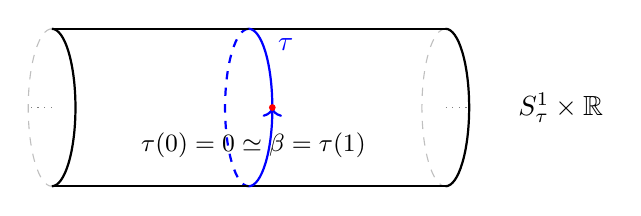
\begin{tikzpicture}[rotate=90]\def\R{1}\def\H{5}\def\zloop{2.5}\def\ry{0.3}\draw[dashed,gray!50](\R,0)arc(0:180:\R cm and \ry cm);\draw[dashed,gray!50] (\R,\H)arc(0:180:\R cm and \ry cm);\draw[blue,thick,dashed](\R,\zloop)arc(0:180:\R cm and \ry cm);\draw[thick](-\R,0)--(-\R,\H);\draw[thick](\R,0)--(\R,\H);\draw[thick](\R,0)arc(0:-180:\R cm and \ry cm);\draw[thick](\R,\H)arc(0:-180:\R cm and \ry cm);\draw[blue,thick,->](-\R,\zloop)arc(180:270:\R cm and \ry cm);\draw[blue,thick](0,\zloop-\ry)arc(270:360:\R cm and \ry cm);\filldraw[red](0,\zloop-\ry)circle(1pt);\node[below=.2]at(0,\zloop-\ry*.2){\small$\tau(0)=0\simeq\beta=\tau(1)$};\node[blue,right]at(\R*0.8,\zloop*0.9){$\tau$};\draw[gray,dotted](0,\H)--(0,\H+0.3);\draw[gray,dotted](0,0)--(0, -0.3)node[black,right=.5]{$S^1_\tau\times\mathbb{R}$};\end{tikzpicture}\captionof{figure}{一维空间$\mathscr M^{}_E=S^1_\tau\times\mathbb{R}$虚时圆的结构示意图}\label{yiDF--shu}\end{center}
%对于二维空间$\mathscr M^{}_E=S^1_\tau\times\mathbb{R}^2$的虚时圆,这是比较难画的,因为既要保证虚时圆和平面相交的点不变,又要确保所有圆的周长相同。因此这个结构就不展示了,留给读者自行思考,全流形$\mathscr M^{}_E=S^1_\tau\times\mathbb{R}^3$同样。\\
%\\
%基于上述理论,我们对温度有了一个全新的认知:$T=1/\beta=1/P\qty(S^1_\tau)$为虚时圆的周长倒数。因此零温理论$T=0$对应$P\qty(S^1_\tau)=\infty$,说明虚时圆被拉伸为一条直线,这就是真实时间轴$t$;而对于无限大温度$T=\infty$,我们得到$P\qty(S^1_\tau)=0$,这说明虚时圆退化为一个点,只留下空间部分,对应均分定理。并且我们还能解释式(\ref{Adigon-*SD})中的$3+1$分解,事实上超曲面$\Sigma^{}_\tau=\mathbb R^3$,它和$\tau$无关,这和真实时空的分解完全不同,因为其体现热静系的\textsl{Gallile}性。\\
%\\
%虽然时空流形相较零温场发生了变化,但在理论形式上并没有区别,因为根据\textsl{Wick}旋转定义的解析延拓,它并没有改变形式。于是我们可以照搬第\ref{laozud}节的内容,对于实标量场$\psi$,在$\mathscr M^{}_E$上引入关于外场$J$的生成函数,方便起见下面我们只写出宗量$\tau$
%\begin{equation}Z(J;\beta)=\bigointsss_{\mathcal C}\mathscr D\psi(\tau)\exp(-\int_0^\beta\dd\tau\int_{\mathbb R^3}\dd V\qty[\Lambda^{}_E[\psi]-J(\tau)\psi(\tau)]).\label{yf][]]=-=bUV}\end{equation}
%这里对场位形不加上\textsl{Matsubara}记号,于是我们得到温度\textsl{Green}函数
%$$C^M\qty(\tau^{}_1,\tau^{}_2)=\frac{1}{Z(\beta)}\eval{\qty(\pdv{Z(J;\beta)}{J\qty(\tau^{}_1)}{J\qty(\tau^{}_2)})}_{J=0}=\frac{1}{Z}\int\mathscr D\psi(\tau)\psi(\tau^{}_1)\psi(\tau^{}_2)\exp(-S^{}_E[\psi]),$$
%以及温度多点函数
%$$C^M\qty(\tau^{}_1,\tau^{}_2,\ldots)=\frac{1}{Z(0)}\eval{\qty(\pdv{(-J)\qty(\tau^{}_1)}\pdv{(-J)\qty(\tau^{}_2)}\cdots)Z(J;\beta)}_{J=0}.$$
%而如果我们同样从宏观运动方程讨论,按照式(\ref{gJiGVa-cc})平移得到场位形
%$$\psi^{}_f\qty(\tau^{}_x)=\psi-\psi^{}_0=\psi\qty(\tau^{}_x)-\int_0^\beta\dd\tau^{}_y\int G\qty(\tau^{}_x,\tau^{}_y)J^{}_y\dd V^{}_y,$$
%则做类似的计算,我们从式(\ref{sehuirzwz})得到热\textsl{KG}场的生成函数
%\begin{equation}Z(J;\beta)=Z(\beta)\exp{\dfrac{1}{2}\int_0^\beta\dd\tau^{}_x\dd\tau^{}_y\int J^{}_xD^M_F\qty(\tau^{}_x,\tau^{}_y)J^{}_y\dd V^{}_x\dd V^{}_y}.\end{equation}
%我们同样可以对应第\ref{eteRT--hh}节的内容,计算变分$\delta\expval{\psi(\tau^{}_a)}=0$,则我们根据式(\ref{eRnfYb-*//})得到温度\textsl{Feynman}传播子的接触项
%\begin{equation}\begin{aligned}&-\frac{1}{Z(\beta)}\qty(\pdv[2]{\tau_x}+\bm{\Delta}^{}_x)\int\psi\qty(\tau^{}_x)\psi\qty(\tau^{}_a)e^{-S^{}_E[\psi(\tau)]}\mathscr D\psi(\tau)\\&=-\qty(\pdv[2]{\tau_x}+\bm{\Delta})\expval{\mathbb T^M\qty{\hat{\psi}(\tau^{}_x)\hat{\psi}(\tau^{}_a)}}=\delta(\tau^{}_x-\tau^{}_a)\delta^3(\vb{x}-\vb{r}^{}_a).\end{aligned}\end{equation}
%这里只需要带入\textsl{Wick}旋转即可,可见在接触点处的结构不变,并且热\textsl{SD}方程由式(\ref{hu7t54nm7})给出
%\begin{equation}\expval{\mathbb T^M\qty{\delta^{}_{\psi}\hat{\Lambda}^{}_E[\psi(\tau)]\hat{\psi}^M_1\cdots\hat{\psi}^M_n}}=-\sum_k\expval{\mathbb T^M\qty{\hat{\psi}^M_1\cdots\hat{\psi}^M_{k-1}\delta^{}_{kx}\hat{\psi}^M_{k+1}\cdots\hat{\psi}^M_n}}.\end{equation}
%此处$\delta^{}_{\psi}$仍是\textsl{EL}导数,注意\textsl{EL}方程现在也建立在$\mathscr M^{}_E$上,所以该导数也需要改为欧式形式。但是由于接触点已经处于欧式度规,因此热\textsl{SD}方程在形式上不变。\\
%\\
%最后我们来证明\textsl{BdD}定理,但根据之前的结论,实际上我们完全可以从第\ref{eteRT--hh}节中,利用接触点得到。比如对于温度两点函数,记\textsl{EL}导数给出算符$\hat{\mathcal D}^{}_E$,我们写出
%$$C^M\qty(\tau^{}_1,\tau^{}_2)=-\int_0^\beta\int C^M\qty(\tau^{}_x,\tau^{}_1)\hat{\mathcal D}^{}_E\expval{\mathbb T^M\qty{\hat{\psi}^M_x\hat{\psi}^M_2}}\dd\tau^{}_x\dd V^{}_x,$$
%从而温度四点函数
%$$D^M\qty(\tau^{}_1,\tau^{}_2,\tau^{}_3,\tau^{}_4)=-\int_0^\beta\int C^M\qty(\tau^{}_1,\tau^{}_x)\hat{\mathcal D}^{}_E\expval{\mathbb T^M\qty{\hat{\psi}^M_x\hat{\psi}^M_2\hat{\psi}^M_3\hat{\psi}^M_4}}\dd\tau^{}_x\dd V^{}_x.$$
%此时热\textsl{SD}方程给出
%$$\hat{\mathcal D}^{}_xD^M(\tau^{}_x,\tau^{}_2,\tau^{}_3,\tau^{}_4)=-\qty{\delta^{}_{x2}C^M(\tau^{}_3,\tau^{}_4)+\delta^{}_{x3}C^M(\tau^{}_2,\tau^{}_4)+\delta^{}_{x4}C^M(\tau^{}_2,\tau^{}_3)},$$
%带入后我们得到
%\begin{equation}D^M\qty(\tau^{}_1,\tau^{}_2,\tau^{}_3,\tau^{}_4)=C^M\qty(\tau^{}_1,\tau^{}_2)C^M(\tau^{}_3,\tau^{}_4)+C^M\qty(\tau^{}_1,\tau^{}_3)C^M(\tau^{}_2,\tau^{}_4)+C^M\qty(\tau^{}_2,\tau^{}_3)C^M(\tau^{}_1,\tau^{}_4).\end{equation}
%更多点的关联函数就不再介绍了,同样也可以得到,只有偶数点关联函数允许存在。其余的内容就不再介绍了,可以参考前文的零温理论,做\textsl{Wick}旋转即可,事实上这些性质是由解析延拓所保证的。
%\subsection{非平衡自由热场}
%\noindent 前面我们考察了平衡态的虚时理论,并将\textsl{Matsubara}绘景理解为关于热态的正则系综均值。现在我们回到真实时间$t$,来讨论在有限温度场中,和$t$相关的热态统计。这里涉及非平衡统计物理,此处我们只是以一个简单的模型,来建立基本的场论框架。
%\subsubsection{演化的闭合时间路径}\label{oeERgYGGG-*-*-/}
%\noindent 在平衡态中,正则系综的密度矩阵由算符$\hat{\vb{w}}=Z^{-1}\exp(-\beta \hat{H})$确定,其和时间无关。现在我们假设,在$t=0$时刻系统处于平衡态$\hat{H}^{}_0$中,当$t>0$时处于$\hat{H}(t)$中,$\hat{H}(t)\neq\hat{H}^{}_0$。这意味着初始$\hat{\vb{w}}(0)$是由$\hat{H}^{}_0$的热态构成,在能量表象下写作
%$$\hat{\vb{w}}(0)=\sum_{n^{}_0}\int \dyad{n^{}_0,\xi}{n^{}_0,\xi}\dd\xi,\quad \hat{H}^{}_0\ket{n^{}_0}=E^{}_0\ket{n^{}_0},$$
%但这并不对应$\hat{H}(t>0)$的热态。为此我们需要考虑密度矩阵关于$\hat{H}$的演化,而这正是非平衡的体现。\\
%\\
%方便起见,我们考察平衡态之间的突变,假设$\hat{H}$和时间无关。根据方程(\ref{vonNeumann1}),我们很容易的得到含时密度矩阵的形式
%\begin{equation}\hat{\vb{w}}(t)=\hat{\tau}(t)\hat{\vb{w}}(0)\hat{\tau}^\dagger(t),\quad \hat{\tau}=\exp(-i\hat{H}t).\end{equation}
%我们也可以通过能量表象下的形式得到:
%$$\hat{\vb{w}}(t)=\sum_{n^{}_0}\int \dyad{n^{}_0,\xi,t}{n^{}_0,\xi,t}\dd\xi=\sum_{n^{}_0}\int \hat{\tau}(t)\dyad{n^{}_0,\xi}{n^{}_0,\xi}\hat{\tau}^\dagger(t)\dd\xi=\hat{\tau}(t)\hat{\vb{w}}(0)\hat{\tau}^\dagger(t).$$
%从上式可以直观的看到,实际上含时密度矩阵处于\textsl{Schrödinger}绘景,这和一般的二次量子化算符是不同的。这也就是为什么在第\ref{98ujo}节中,着重强调单粒子约化密度矩阵算符$\hat{\bm{\zeta}}^{(a)}\neq\hat{\vb{w}}$的原因,因为$\hat{\bm{\zeta}}^{(a)}$是可观测的,其在\textsl{Heisenberg}绘景中演化。因此对于初态的\textsl{Schrödinger}算符$\hat{f}$,其均值为
%\begin{equation}\expval{\hat{f}}(t)=\tr{\hat{f}(0)\hat{\vb{w}}(t)}=\tr{\hat{\vb{w}}(0)\hat{\tau}^\dagger(t)\hat{f}(0)\hat{\tau}(t)}=\tr{\hat{\vb{w}}(0)\hat{f}(t)},\end{equation}
%也就是说非平衡系统中,单个算符的均值在形式上,和平衡态的演化均值没有区别,只不过在平衡态中通过遍历定理将时间也平均了,因而最终的均值和时间无关。\\
%\\
%现在我们来考察\textsl{Green}函数,这是非平衡态和平衡态最主要的不同点。由于\textsl{Green}函数是在\textsl{Heisenberg}绘景中计算的,此时态不演化,因而我们依旧可以按零温场定义,比如对于实标量场有
%\begin{equation}C(x,y)=\expval{\mathbb T\qty{\hat{\psi}^\dagger(x)\hat{\psi}(y)}}=\tr{\hat{\vb{w}}(0)\mathbb T\qty{\hat{\psi}^\dagger(x)\hat{\psi}(y)}}.\end{equation}
%现在假设$x^0<y^0$,则我们写出\textsl{Schrödinger}绘景中的\textsl{Green}函数的
%$$\begin{aligned}C(x,y)&=\tr{\hat{\vb{w}}(0)\hat{\tau}^\dagger\qty(y^0)\hat{\psi}(\vb{y})\hat{\tau}\qty(y^0)\hat{\tau}^\dagger\qty(x^0)\hat{\psi}(\vb{x})\hat{\tau}\qty(x^0)}\\&=\tr{\hat{\tau}\qty(x^0)\hat{\vb{w}}(0)\hat{\tau}^\dagger\qty(y^0)\hat{\psi}(\vb{y})\hat{\tau}\qty(y^0)\hat{\tau}^\dagger\qty(x^0)\hat{\psi}(\vb{x})}.\end{aligned}$$
%对于$x^0>y^0$,我们得到
%$$C(x,y)=\tr{\hat{\tau}\qty(y^0)\hat{\vb{w}}(0)\hat{\tau}^\dagger\qty(x^0)\hat{\psi}(\vb{x})\hat{\tau}\qty(x^0)\hat{\tau}^\dagger\qty(y^0)\hat{\psi}(\vb{y})}.$$
%可见此时\textsl{Green}函数不是均匀的,从而无法使用零温场的周期边界定义。对于纯态零温场$\hat{\vb{w}}(0)=\hat{\vb{I}}$,说明函数只和时间差$t=x^0-y^0$有关,因此周期边界可以任意定义,而这里由于$\hat{\vb{w}}$的插入,使得这种对称性的丢失。或者也可以说,由于现在系统由固定的初态,因此基于周期边界最终位形的取值要回到初态,这导致自发的时间对称性破缺。\\
%\\
%为了解决这个问题,我们不妨从路径积分着手,因为其不依赖时序的定义。对于热实标量场,我们按迹的积分形式写出
%\begin{equation}Z=\bigointsss_{C^*} \exp(i\int\Lambda(\psi)\dd\Omega-\beta H^{}_0(\psi))\mathscr D\psi(t,\vb{r}),\label{As..x*/xXX}\end{equation}
%其中$C^*$是$\psi$在位形空间$\mathscr C$中的闭合回路。参照热平衡场,我们对时间引入参数曲线$\gamma(u)=(t(u),\vb{r}(u))$,假设$H^{}_0=0$,此时回路$C^*$和虚时圆$S^1_\tau$一样给出
%$$t(0)=t^{}_i=t(1),\quad\vb{r}(0)=\vb{r}(1),\quad H^{}_0=0.$$
%但热场中$H^{}_0\neq0$,现在若假设真实时间$t\in\mathbb C$,则按照\textsl{Wick}旋转我们可以将统计部分写作
%$$-\beta H^{}_0=-iH^{}_0(-i\beta)=-iH^{}_0(t^{}_i-i\beta-t^{}_i)=-i\int_{t^{}_i}^{t^{}_i-i\beta} H^{}_0\dd t.$$
%另一方面,如果我们将\textit{Hamiltonian}定义为一个分段函数
%\begin{equation}H=\begin{cases}H^{}_0=const,\quad -\infty<t\leq 0;&\\ H=const,\quad 0<t<\infty,\end{cases}\end{equation}
%则初态的平衡统计部分可以作为守恒能量,利用\textsl{HJ}定理纳入作用量积分中,给出
%\begin{equation}S=\int_{t^{}_i}^{t^{}_i-i\beta}\dd t \int\dd V\Lambda[\psi(\gamma)].\end{equation}
%当然现在依然有$\vb{r}(0)=\vb{r}(1)$,因而我们不妨只考察时间部分,根据定义$t(u)\in \mathbb C$是复平面中的曲线,不妨按一般的复数记号记为$z(u)$,其两个端点为
%\begin{equation}z(0)=t^{}_i,\quad z(1)=t^{}_i-i\beta.\end{equation}
%也就是说,现在位形回路$C^*$给出一条不封闭的复时间曲线。还是参考虚时圆,我们在复平面中定义等价关系$z(0)\sim z(1)$,则重新定义曲线为商空间$z(u)=z(u)/\sim$,这是一条$\mathbb C$中的封闭曲线。当然这是非物理的结论,因为真实时间只能取实数,所以我们需要进一步处理。\\
%\\
%现在我们来研究其性质,以及如何构造这条回路$^{\cite{therFUrc}}$。对于复数时间$t$,可以想到初态作为平衡态满足\textsl{KMS}条件(\ref{KOm-*-*-gI087}),即热平衡\textsl{Green}函数的解析延拓$G(z)=G(z+i\beta),\ z\in\mathbb C$。取
%$$z=t^{}_i-i\beta\implies G(t^{}_i-i\beta)=G(t^{}_i)\implies t^{}_i\sim t^{}_i-i\beta,$$
%这就证明了等价关系$z(0)\sim z(1)$的正确性,从而商空间$z(u)$是虚时圆$S^1_\tau$在复平面上的扩展。现在不加证明的将\textsl{KMS}条件推广至真实时间$t$,因为其为实数那么不妨定义$t=\Re z$,由\textsl{Wick}旋转可以将$z$定义为
%\begin{equation}t'=-i\tau\implies z=t+t'=t-i\tau,\quad t,\tau\in\mathbb R.\end{equation}
%在平衡态中,虚时$\tau$的取值为$0\leq\tau\leq\beta$,\textsl{KMS}条件将其延拓至$-\beta\leq\tau\leq0$。现在我们将这个条件理解为$z$的虚部,并将复变\textsl{Heaviside}函数写作虚实部的乘积给出
%\begin{equation}\theta(z)=\theta(t)\theta(-\tau)\implies\Im z=-\tau\in[-\beta,0]\quad\theta(-z)=\theta(-t)\theta(\tau)\implies\Im z\in[0,\beta].\end{equation}
%对\textsl{Green}函数的编时乘积$\mathbb T$展开,并直接将$t$延拓为$z$给出
%\begin{equation}G(z^{}_1,z^{}_2)=\expval{\hat{\psi}\qty(z^{}_1)\hat{\psi}\qty(z^{}_2)}\theta(z)+\expval{\hat{\psi}\qty(z^{}_2)\hat{\psi}\qty(z^{}_1)}\theta(-z),\quad z=z^{}_2-z^{}_1,\label{diFRWER55090)()(}\end{equation}
%现在证明该延拓的合理性:由于上式同时包含复变\textsl{Heaviside}函数$\theta(z)$和$\theta(-z)$,所以\textsl{Green}函数的定义域应满足
%\begin{equation}[-\beta,0]\cup[0,\beta]=\qty{0}=\Im z,\label{;dkd-*-*..ggh}\end{equation}
%也就是说从$t^{}_i\in\mathbb R$出发,这个函数完全定义在实轴上,符合要求。于是从初始平衡态$t^{}_i$出发,$z(u)$在$\mathbb R$上的部分可以按零温场的周期边界定义,取$t^{}_i=-\mathfrak T$为
%$$\mathcal P^{}_1(u)=(-\mathfrak T,\mathfrak T)\subset z(u),\quad z(0)=-\mathfrak T\longrightarrow\mathfrak T=z(u>0), \quad\mathfrak T\to\infty.$$
%此时\textsl{Green}函数$C(x,y)$的时间应该满足$x^0,y^0\in \mathcal P^{}_1(u)$,场位形算符的编时乘积按照$u$的大小确定。注意现在曲线$z(u)$的终点为$z(1)=-\mathfrak T-i\beta$。\\
%\\
%但我们知道$z(u)$是回路,因此现在要解决的就是如何从$\mathfrak T$回到$-\mathfrak T-i\beta$。首先注意到,我们不能直接从$\mathfrak T$取直线回到$-\mathfrak T-i\beta$,因为\textsl{Green}函数虽然可以在上面定义,但不一定解析,这是一个非物理的选择。为了解决这个问题,我们先推广条件(\ref{;dkd-*-*..ggh}),根据\textsl{KMS}条件(\ref{KOm-*-*-gI087}),取$z=t+ib$我们得到
%$$G(t+ib)=\mp G(t+i(b+\beta)),\forall b\in\mathbb R.$$
%这说明对于任意的虚部$b$,平衡态的虚时范围$0\leq\tau\leq\beta$都可以延拓为为$-\beta\leq\tau\leq0$,因而延拓式(\ref{diFRWER55090)()(})的定义域仍应满足
%\begin{equation}[-\beta,0]\cup[0,\beta]=\qty{0}=b\implies \Im z=const,\quad \Re z=t(u).\label{ji+Jrt''lu}\end{equation}
%因此我们看到,复\textsl{Green}函数$G(z)$若要在实部变化的情况下保持解析,则只要求$\Im z=const$即可,它扩充了条件(\ref{;dkd-*-*..ggh})。现在我们假定$t=\mathfrak T$时系统处于准静态,因为它不是真实的平衡态,所以不能直接沿实轴返回,但可以在平衡态下定义等价关系$\mathfrak T\sim\mathfrak T-i\epsilon$使其和实轴分开,并在虚轴上给出虚时圆
%$$\Im z=S^1_\epsilon=[\mathfrak T-0,\mathfrak T-i\epsilon]/{0\sim\epsilon}.$$
%由于这是准静态,因此应添加约束$\epsilon\to0$,这对应了第\ref{wta665bbgl}节中零温场时间的微虚性。将$\mathfrak T-i\sigma$作为当前的初始时刻,基于结论(\ref{ji+Jrt''lu}),为了令$G(z)$解析需保持$\sigma$不变,这就给出一条和实轴平行但不同的直线
%$$\mathcal P^{}_2(u)=\lim_{\epsilon\to0}(\mathfrak T-i\epsilon,-\mathfrak T-i\epsilon)\subset z(u),\quad z\qty(u^{}_1)=\mathfrak T-i\epsilon\longrightarrow-\mathfrak T-i\epsilon=z\qty(u^{}_2>u^{}_1).$$
%接下来再取路径$-\mathfrak T-i\epsilon\longrightarrow-\mathfrak T-i\beta$,并在平衡态下做等价,我们就完成了回路的最后一段
%$$\Im z=S^1_\beta=-\mathfrak T-i\epsilon\longrightarrow-\mathfrak T-i\beta\sim-\mathfrak T\subset z(u).$$
%由于终点$-\mathfrak T-i\beta$按照定义是平衡态时间,所以上述线段是一个虚时圆,当然应当强调的是这是一个真实的\textsl{Matsubara}虚时圆,和为了与实轴区分而做的微虚段$S^1_\epsilon$不同。\\
%\\
%将上述两个虚时圆记为$\mathcal P^{}_2=S^1_\epsilon$,$\mathcal P^{}_4=S^1_\beta$,则整个回路按参数$u$的增加定义为
%\begin{equation}z(u)=\mathcal P^{}_1+\mathcal P^{}_3+\mathcal P^{}_2+\mathcal P^{}_4.\end{equation}
%按照上述构造方法定义的复时间回路$z(u)$称为\textbf{\textsl{Konstantinov-Perel}路径},复\textsl{Green}函数$G(z)$在其上是处处解析的,复平面上展示为图 \ref{weGBNNM..,te}
%\begin{center}\tikz{\tikzset{mid arrow/.style={postaction={decorate,decoration={markings,mark=at position #1 with{\arrow{Stealth}}}}},mid arrow/.default=0.5}\def\phi{3.5}\def\sigmaOffset{-.7}\def\betaOffset{-2.5}\def\eps{0.01}\draw[->,>=Stealth,gray,thin](-\phi-1,0)--(\phi+1,0)node[right,black]{$\Re z=t$};\draw[->,>=Stealth,gray,thin](0,\betaOffset-0.5)--(0,1.0)node[below right,black]{$\Im z=\tau$};\draw[mid arrow,thick](-\phi,\eps)--(\phi,\eps)node[above left,midway]{$\mathcal P^{}_1$};\filldraw(-\phi,\eps)circle(1.2pt)node[above,black]{$-\mathfrak T$};\filldraw(\phi,\eps)circle(1.2pt)node[above,black] {$\mathfrak T$};\draw[mid arrow=0.7,thick](\phi,\eps)--(\phi,\sigmaOffset)node[right,midway,font=\small]{$\mathcal P^{}_3$};\filldraw(\phi,\sigmaOffset)circle(1.2pt) node[below, black]{$\mathfrak T-i\epsilon$};\draw[mid arrow,thick](\phi,\sigmaOffset)--(-\phi,\sigmaOffset)node[below right,midway]{$\mathcal P^{}_2$};\filldraw(-\phi,\sigmaOffset)circle(1.2pt) node[above,black]{$-\mathfrak T-i\epsilon$};\draw[mid arrow,thick](-\phi,\sigmaOffset)--(-\phi,\betaOffset)node[right,midway,font=\small]{$\mathcal P^{}_4$};\filldraw(-\phi,\betaOffset)circle(1.2pt)node[below,black]{$-\mathfrak T-i\beta$};\draw[mid arrow,bend left=60,dashed] (-\phi,\betaOffset)to node[left,midway]{$S^1_\beta$}(-\phi,\eps);}\captionof{figure}{\textsl{Konstantinov-Perel}路径$z(u)$的构造。}\label{weGBNNM..,te}\end{center}
%从图中可以看到,$\mathcal P^{}_3$和$\mathcal P^{}_4$这两条是纯虚路径,对应平衡态的虚时圆,它们不会给出任何关于非平衡演化的信息。因此在具体计算时,通常会省略这两个分支,在等价关系下我们得到商空间
%\begin{equation}z(u)/\sim=\mathcal P^{}_1+\qty(\mathcal P^{}_3=\expval{\mathfrak T})+\mathcal P^{}_2+\qty(\mathcal P^{}_4=\expval{-\mathfrak T})=\mathcal P^{}_1+\mathcal P^{}_2.\end{equation}
%因为$\mathcal P^{}_1$和$\mathcal P^{}_2$的始末点对偶等价,且因为$\epsilon\to0$因此这个构造可以看作在$\mathbb R$的回路,但注意始末点和转折点为$\pm\infty$。称此商空间对应的时间路径$z(u)/\sim$为\textbf{闭合时间路径 \textit{Closed Time Path}},或简称\textbf{\textsl{CTP}}。但需要注意,这是从\textsl{KP}路径简化而来的,是为了计算方便而做的构造,其中$\mathcal P^{}_1\neq -\mathcal P^{}_2$,绝不能简单的看作$\mathbb R$上两个相反的路径,其中一条需要在等价关系下微虚。\\
%\\
%事实上我们可以从复合路径的角度理解,将商空间记为
%\begin{equation}z(u)/\sim=\begin{cases}\mathcal P^{}_1,\quad 0\leq u\leq 1/2;&\\ \mathcal P^{}_2,\quad 1/2\leq u\leq 1.\end{cases}\label{8*/SFG/*---}\end{equation}
%这样一来,我们从参数上完全区分了这两条路径,并且这个回路是连续的,其在$u=1/2$处的连续性由等价关系保证。虽然$\mathcal P^{}_2$同样是实轴$\mathbb R$,但是对于同一时刻$t^{}_0$,它可以是$t^{}_0=z(0.2)/\sim\in\mathcal P^{}_1\neq z(0.8)/\sim\in\mathcal P^{}_2$。这个理解在具体计算层面是非常有帮助的,在理解了这一点后,\textsl{CTP}的构造其实就是道路的乘积法则。
%\subsubsection{Schwinger-Keldysh理论和Keldysh张量}
%\noindent 在定义了\textsl{CTP}之后,我们来处理非平衡场的热\textsl{Green}函数。由于\textsl{CTP}在等价关系下简化为$\mathbb R$的回路,因此我们不妨记为$t(\sim)=z(u)/\sim=\mathcal P^{}_1+\mathcal P^{}_2$,当然需要注意$\mathcal P^{}_2$在定义上有一定的偏离。根据路径的方向,下面我们称$\mathcal P^{}_1$为正向支,$\mathcal P^{}_2$为反向支。\\
%\\
%首先确定形式,我们之前已经在复平面上得到延拓(\ref{diFRWER55090)()(}),当然其没有任何物理含义。在虚时圆$S^1_\tau$上我们定义了\textsl{Matsubara}乘积序$\mathbb T^M$,在\textsl{CTP}上也可以定义相应的编时乘积$\mathbb T$,由于现在时间构成一个回路,因此我们将其称为\textbf{\textsl{Keldysh}回路乘积},或者\textbf{路径乘积 \textit{Path Ordering Product}},记为$\mathbb P=\mathbb T^{}_{t(u)}$。于是延拓(\ref{diFRWER55090)()(})在实轴上就可以写为
%\begin{equation}C^{K}(x,y)=\expval{\mathbb P\qty{\hat{\psi}^\dagger(x)\hat{\psi}(y)}},\quad x^0,y^0\in\mathbb R\subset \mathcal P^{}_1+\mathcal P^{}_2.\end{equation}
%在相对论中“编时”一词更多的采用\textsl{Chronological}来称呼,对于路径也有相应的术语\textsl{Hodological},所以这两个乘积也可以称为
%$$\mathbb T=\textit{Chronological Product},\quad \mathbb P=\textit{Hodological Product}.$$
%当然\textsl{Hodological}这个术语用的不多,因此在文献中多以\textsl{Path Ordering Product}或者\textsl{Contour Product}称呼,有些文献也会以$\mathbb T^{}_c$表示路径乘积。根据定义和图 \ref{weGBNNM..,te},若$x^0$和$y^0$均在$\mathcal P^{}_1$上,则其上的路径乘积就是通常的编时乘积
%$$\expval{\mathbb P\qty{\hat{\psi}^\dagger(x)\hat{\psi}(y)}}\qty(x^0,y^0\in \mathcal P^{}_1)=\expval{\mathbb T\qty{\hat{\psi}^\dagger(x)\hat{\psi}(y)}},$$
%因为在正向支$\mathcal P^{}_1$上时间是沿正向流动的,和通常的时空定义以及零温场理论没有任何区别。\\
%\\
%其次确定路径乘积$\mathbb P$的具体展开,为此我们不妨从和时序无关的路径积分出发。在\textsl{CTP}的构造下,路径积分(\ref{As..x*/xXX})现在可以忽略$-\beta H^{}_0$部分写作
%$$Z=\oint_{\vb{q}[t(\sim)]} \exp{iS[\vb{q}(t)]}\mathscr D\vb{q}(t),\quad \vb{q}(-\mathfrak T)=\vb{q}(-\mathfrak T-i\beta).$$
%方便起见,这里我们依然只写出时间宗量,并且按照零温场的周期边界依旧取$\mathfrak T=\infty$。此时按照零温场的结论(\ref{uhyg586}),我们得到以路径积分表示的路径乘积下的两点函数,这里用粒子波函数场为例
%\begin{equation}C^K(1,2)=\expval{\mathbb P\qty{\hat{\psi}^{\dagger}_1\hat{\psi}_2}}=\frac{\displaystyle\oint\exp{iS\qty(\psi,\psi^*)}\psi^*_1\psi^{}_2\mathscr D\psi\mathscr D\psi^*}{\displaystyle\oint\exp{iS\qty(\psi,\psi^*)}\mathscr D\psi\mathscr D\psi^*}.\label{D*//FFFU--..H66uhs}\end{equation}
%在平衡态理论中,实$\tau$宗量确定了\textsl{Eculidean}作用量
%$$\displaystyle S^{}_E=\int_0^\beta\dd\tau\int\Lambda^{}_E[\vb{q}(\tau,\vb{r})]\dd V,\quad\tau\in S^1_\tau,$$
%其中$\tau$沿虚时圆积分。在$S^1_\tau$上$\tau$被解释为圆的弧长,$\beta$为整周长,因此对$\tau$的积分依旧是普通\textsl{Riemann}积分。但是\textsl{CTP}的构造有明确的来回方向,所以沿$t(\sim)$的积分是一个回路积分,当然考虑到$\mathcal P^{}_1\neq -\mathcal P^{}_2$所以应分解为两个积分,不妨将沿正向支$\mathcal P^{}_1$参数记为$t^{}_+=t$,反向支$\mathcal P^{}_2$参数记为$t^{}_-=t-i\epsilon$,我们得到
%\begin{equation}\oint_{t(\sim)}\dd t=\int_{\mathcal P^{}_1}\dd t+\int_{\mathcal P^{}_2}\dd t=\int_{\mathbb R}\dd t^{}_++\int_{\mathbb R}\dd t^{}_-.\label{ni--/*HGT++../}\end{equation}
%这说明在计算\textsl{Green}函数时,时间宗量需要按所处曲线分为正负两个变量,这是一个很重要的结论,因为它暗示我们对于两点函数,$\mathbb P$的展开有四种可能的情况,我们后面会看到。现在的作用量应写作
%$$S=\oint_{t(\sim)}\dd t\int\Lambda[\vb{q}(t,\vb{r})]\dd V=\int_{\mathbb R}\dd t^{}_+\int\Lambda[\vb{q}(t,\vb{r})]\dd V+\int_{\mathbb R}\dd t^{}_-\int\Lambda[\psi(t,\vb{r})]\dd V,$$
%若我们按曲线方向记时空体积元$\dd V\dd t^{}_{\pm}=\dd\Omega^{}_{\pm}$,则作用量给出
%\begin{equation}S=S^{}_++S^{}_-=\int\Lambda[\vb{q}(t,\vb{r})]\dd\Omega^{}_++\int\Lambda[\psi(t,\vb{r})]\dd\Omega^{}_-.\label{DaBeSeig}\end{equation}
%现在路径积分写作
%\begin{equation}Z=\oint\exp{iS^{}_+[\vb{q}(t)]}\exp{iS^{}_-[\vb{q}(t)]}\mathscr D\vb{q}(t),\end{equation}
%但这是非常突兀的,因为现在有两个时间宗量,理应对应两个不同的位形。可是在回路积分下,位形并不显含时间方向,因此这两个时间$t^{}_{\pm}$看似没有任何理由,作为两个不同位形各自的宗量。后续我们会看到,实际上两个位形的出现是十分自然的,而这也非平衡的特征。\\
%\\
%现在我们按照通常的程序计算\textsl{Green}函数,不失一般性的这里考察实标量场$\psi$,根据第\ref{laozud}节的结论我们需要引入生成函数
%$$Z(J)=\bigintsss \exp{i\int(\Lambda(\psi)-J\psi)\dd\Omega}\mathscr D\psi(t),$$
%\textsl{Green}函数由其对外场的导数确定
%$$D^{}_F(x,y)=-\frac{1}{Z(0)}\eval{\pdv{Z(J)}{J^{}_x}{J^{}_y}}_{J(x)=0}.$$
%可是由于在\textsl{CTP}下,时空体积元分为两个$\dd\Omega^{}_{\pm}$,因此我们也需要两个外场,记为$J^{}_{\pm}(t)=J\qty(t^{}_{\pm})$,其中$J^{}_+(t)=J(t)$定义在$\mathcal P^{}_1$上,而$J^{}_-(t)=J(t-i\epsilon)$定义在$\mathcal P^{}_2$上。方便起见,我们用指标$l,m=1,2$代表$\pm$号,于是生成函数写作
%\begin{equation}Z^{}_{SK}\qty(J^{}_m;\beta)=\bigointsss\exp{i\sum_{m=1,2}\int\qty[\Lambda(\psi)-J^{}_m\psi]\dd\Omega^{}_m}\mathscr D\psi(t).\label{wuGBNg6//**}\end{equation}
%称这个生成函数为非平衡场的\textbf{\textsl{Schwinger-Keldysh}泛函},其和处于不同方向上的外场相关。定义\textsl{CPT}上两个外场之间的导数为
%\begin{equation}\fdv{J^{}_l(x)}{J^{}_m(y)}\simeq\pdv{J^{}_l(x)}{J^{}_m(y)}=\delta^{m}_l\delta^4_{xy},\quad x,y\in t(\sim),\label{wuNlog656}\end{equation}
%则我们得到相应的热\textsl{Green}函数
%\begin{equation}C^{lm}(x,y)=-\frac{1}{Z^{}_{SK}(0;\beta)}\eval{\pdv{Z^{}_{SK}\qty(J^{}_l;\beta)}{J^{}_l(x)}{J^{}_m(y)}}_{J^{}_m=0},\quad l,m=1,2.\label{zIDH9*9899***iyh}\end{equation}
%称$C^{lm}(x,y)$为\textbf{\textsl{Keldysh}张量},容易证明$C^{lm}(x,y)$是一个二维二阶逆变张量,这是条件(\ref{wuNlog656})保证的。取指标$l=1=+$,$l=2=-$,则我们得到一个二维\textsl{Green}函数矩阵
%\begin{equation}\vb{C}^K=\mqty(C^{++}&C^{+-}\\C^{-+}&C^{--}).\end{equation}
%这个矩阵确定了非平衡场的所有基本性质,在此基础上建立的有限温度场论称为\textbf{\textsl{Schwinger-Keldysh}形式 \textit{Schwinger-Keldysh Formalism}} (\textsl{J. S. Schwinger},\textsl{\rusa{Л. В. Келдыш}},1964)。需要强调的是,由于\textsl{CTP}是\textsl{KP}路径的商空间,而\textsl{KP}路径的终点是$-\mathfrak T-i\beta$,所以\textsl{SK}泛函一定和$\beta$有关,这是有限温度场之所以和零温场不同的根本。\\
%\\
%在\textsl{Keldysh}张量下,我们就可以详细的写出$\mathbb P$的展开了,这里对矩阵元逐一分析。首先是$C^{++}$,根据定义其写作
%$$C^{++}(x,y)=\frac{-1}{Z^{}_{SK}(0;\beta)}\eval{\pdv{Z^{}_{SK}\qty(J^{}_+;\beta)}{J^{}_+(x)}{J^{}_+(y)}}_{J^{}_+=0}.$$
%由于$J^{}_+\in C^\infty\qty(\mathcal P^{}_1)$,因此根据我们之前的分析,它就是通常的\textsl{Green}函数
%\begin{equation}C^{++}(x,y)=\expval{\mathbb T\qty{\hat{\psi}(x)\hat{\psi}(y)}}\implies\mathbb P^{}_{\mathcal P^{}_1}=\mathbb T.\label{itGjjF0O--98}\end{equation}
%对于另一个对角元$C^{--}$,其定义为
%$$C^{--}(x,y)=\frac{-1}{Z^{}_{SK}(0;\beta)}\eval{\pdv{Z^{}_{SK}\qty(J^{}_-;\beta)}{J^{}_-(x)}{J^{}_-(y)}}_{J^{}_-=0}.$$
%由于$J^{}_-\in C^\infty\qty(\mathcal P^{}_2)$,在$\mathcal P^{}_2$上时间是反向流动的,比如$z\qty(u^{}_i)=t^{}_i$,使得$u^{}_1>u^{}_2\implies t^{}_1<t^{}_2$,因此$\mathcal P^{}_2$上的时序和$\mathcal P^{}_1$上的正时序是相反的。按照十卷《物理动理学》\cite{Ld3k}中的记号,我们定义\textbf{反时序乘积 \textit{Anti-Chronological Product}}为
%\begin{equation}\mathbb P^{}_{\mathcal P^{}_2}=\tilde{\mathbb T},\quad \tilde{\mathbb T}\qty{\hat{\psi}(t=0)\hat{\psi}(t>0)}=\hat{\psi}(0)\hat{\psi}(t),\end{equation}
%这个反时序乘积可以理解为:沿$\mathcal P^{}_2$演化的算符,其必然先经过大时间值$t>0$,再经过小时间值$t=0$,因此是大时间值算符$\hat{\psi}(t)$先作用,小时间值算符$\hat{\psi}(0)$后作用,给出$\hat{\psi}(0)\circ\hat{\psi}(t)$。于是我们得到此对角元为
%\begin{equation}C^{--}(x,y)=\expval{\tilde{\mathbb T}\qty{\hat{\psi}(x)\hat{\psi}(y)}}=\expval{\hat{\psi}(x)\hat{\psi}(y)}\theta(y^0-x^0)+\expval{\hat{\psi}(y)\hat{\psi}(x)}\theta(x^0-y^0).\end{equation}
%我们重点分析斜对角元,对于$C^{12}=C^{+-}$写出
%$$C^{+-}(x,y)=\frac{-1}{Z^{}_{SK}(0;\beta)}\eval{\pdv{Z^{}_{SK}\qty(J^{}_+,J^{}_-;\beta)}{J^{}_+(x)}{J^{}_-(y)}}_{J^{}_m=0}.$$
%根据式(\ref{8*/SFG/*---}),在$\mathcal P^{}_2$上的时间永远比$\mathcal P^{}_1$上的大,也就是说沿着$t(\sim)$运动,永远是先经过算符$\psi(\mathcal P^{}_1)$再经过算符$\psi(\mathcal P^{}_2)$,给出$\psi\qty(\mathcal P^{}_2)\circ\psi\qty(\mathcal P^{}_1)$,其中没有时序的概念。所以根据外场所处的曲线,得到$x^0\in \mathcal P^{}_1$,$y^0\in \mathcal P^{}_2$,进而我们得到此混合元为
%\begin{equation}C^{+-}(x,y)=\expval{\hat{\psi}(y)\hat{\psi}(x)},\quad x^0\in \mathcal P^{}_1,\quad y^0\in \mathcal P^{}_2.\end{equation}
%另一个混合元为
%$$C^{-+}(x,y)=\frac{-1}{Z^{}_{SK}(0;\beta)}\eval{\pdv{Z^{}_{SK}\qty(J^{}_+,J^{}_-;\beta)}{J^{}_-(x)}{J^{}_+(y)}}_{J^{}_m=0},$$
%根据上面的分析不难得到
%\begin{equation}C^{-+}(x,y)=\expval{\hat{\psi}(x)\hat{\psi}(y)},\quad x^0\in \mathcal P^{}_2,\quad y^0\in \mathcal P^{}_1.\end{equation}
%在零温场论中,这两个\textsl{Green}函数称为\textbf{\textsl{Wightman}函数},下面我们仍然使用该术语。至此我们得到了所有的四个分量,并给出了路径乘积$\mathbb P$的具体展开,这里简单总结一下
%\begin{equation}\vb{C}^K(x,y)=\mqty(\expval{\mathbb T\qty{\hat{\psi}(x)\hat{\psi}(y)}}&\expval{\hat{\psi}(y)\hat{\psi}\qty(x\in \mathcal P^{}_1)}\\ \expval{\hat{\psi}(x)\hat{\psi}\qty(y\in \mathcal P^{}_1)}&\expval{\tilde{\mathbb T}\qty{\hat{\psi}(x)\hat{\psi}(y)}}).\label{sudg67657--=}\end{equation}
%注意两个斜对角的\textsl{Wightman}函数,这里只标注了对于右侧先作用的算符,其时间宗量永远定义在$\mathcal P^{}_1$上,另一个定义在$\mathcal P^{}_2$上,它们不涉及时序乘积。\\
%\\
%基于这个形式,我们可以回答之前的问题:场位形能否按回路方向分解。答案是可以,因为矩阵的分量完全由位形所处的时间方向决定,所以我们不妨引入两个场位形
%\begin{equation}\psi^{}_+(t)=\psi\qty(t\in\mathcal P^{}_1),\quad\psi^{}_-(t)=\psi\qty(t\in\mathcal P^{}_2),\end{equation}
%\emph{使得每个分量在各自的路径上和零温场位形的性质一样}。则矩阵(\ref{sudg67657--=})可以写作
%\begin{equation}\vb{C}^K(x,y)=\mqty(\expval{\mathbb T\qty{\hat{\psi}^{}_+(x)\hat{\psi}^{}_+(y)}}&\expval{\hat{\psi}^{}_-(y)\hat{\psi}^{}_+\qty(x)}\\ \expval{\hat{\psi}^{}_-(x)\hat{\psi}^{}_+\qty(y)}&\expval{\tilde{\mathbb T}\qty{\hat{\psi}^{}_-(x)\hat{\psi}^{}_-(y)}}).\end{equation}
%这样我们在记号上就明确了每一个分量,并且分量指标也可以轻松的确定,第$n$个正负号由第$n$个坐标所对应的场位形正负号给出,比如矩阵元$C^{21}(x,y)=C^{-+}\qty(x^{}_-,y^{}_+)$。按照这个定义,我们可以得到两个\textsl{Wightman}函数之间的关系
%\begin{equation}C^{-+}(x,y)=\expval{\hat{\psi}^{}_-(x)\hat{\psi}^{}_+(y)}=C^{+-}(y,x).\label{g++FSG-++++hfs}\end{equation}
%也就是说,若变量和符号同时对换,则\textsl{Wightman}函数不变,这是容易证明的,留给读者自行分析。在该记号下,我们也可以将时间方向指标从体元中提出,回到时间积分的分解式(\ref{ni--/*HGT++../}),按照\textsl{Riemanna}积分的定义对$\psi$积分
%$$\oint_{t(\sim)}\psi\dd t=\int_{\mathcal P^{}_1}\psi\dd t^{}_++\int_{\mathcal P^{}_2}\psi\dd t^{}_-=\int_{\mathbb R}\psi^{}_+\dd t+\int_{-\mathbb R}\psi^{}_-\dd t=\int_{\mathbb R}\psi^{}_+\dd t-\int_{\mathbb R}\psi^{}_-\dd t.$$
%这样一来,我们就将不同方向上时间的积分,转化为处于不同路径的场位形的\textsl{Riemanna}时间积分,从而作用量(\ref{DaBeSeig})就写为
%\begin{equation}S=\int\qty{\Lambda[\psi^{}_+(t,\vb{r})]-\Lambda[\psi^{}_-(t,\vb{r})]}\dd\Omega=S^{}_+-S^{}_-.\end{equation}
%注意这里的减号,式(\ref{DaBeSeig})的加号是因为我们改变了积分方向的定义,而这里的减号是\textsl{Riemanna}积分天然的方向,体现为沿\textsl{CTP}的作用量的净增量。此时位形空间为$\bm{\psi}=\mathscr C=\qty{\psi^{}_+,\psi^{}_-}$,因而现在路径积分在形式上和复标量场一样,写作
%\begin{equation}Z^{}_{SK}=\bigintsss\exp(i\int\qty{\Lambda[\psi^{}_+(t,\vb{r})]-\Lambda[\psi^{}_-(t,\vb{r})]}\dd\Omega)\mathscr D\psi^{}_+(t,\vb{r})\mathscr D\psi^{}_-(t,\vb{r}).\end{equation}
%注意\emph{现在不是回路积分},因为根据定义,每个位形在其路径上和零温场理论一样,从$-\infty$演化到$\infty$。此时\textsl{SK}泛函(\ref{wuGBNg6//**})写作
%\begin{equation}Z^{}_{SK}\qty(J^{}_m;\beta)=\bigintsss\exp{iS\qty(\psi^{}_+,\psi^{}_-)-i\sum_{m=1,2}\int J^{}_m\psi^{}_m\dd\Omega}\mathscr D\psi^{}_+\mathscr D\psi^{}_-,\end{equation}
%根据第\ref{eteRT--hh}节最后的部分,我们可以从宏观运动方程的角度,得到以传播子表示的生成函数
%\begin{equation}Z^{}_{SK}\qty(\vb{J}^K;\beta)=Z^{}_{SK}(0)\exp{\int J^{}_l(x)C^{lm}(x,y)J^{}_m(y)\dd\Omega^{}_x\dd\Omega^{}_y}.\label{sgeFCAFC;'p[opk7YT67}\end{equation}
%这实际上对应了零温\textsl{KG}场用\textsl{Feynman}传播子$D^{}_F$表示的生成函数(\ref{sehuirzwz}),两者在形式上是类似的,这进一步体现非平衡态热场和零温场之间的关联。\\
%\\
%当然该记号的便利性不止于此,我们还可以从代数的角度分析。之前提到\textsl{Keldysh}张量是一个二维二阶张量,根据二阶张量的定义,它将一个二维矢量映射为一个二维矢量,参考上面的记号不难想到,这两个二维矢量可以定义为
%\begin{equation}\vb{J}^K=\mqty(J^{}_+\\ J^{}_-)=\qty(J^{}_m)=\qty(J^m),\quad \bm{\psi}^K=\mqty(\psi^{}_+\\ \psi^{}_-)=\qty(\psi^{}_m)=\qty(\psi^m).\end{equation}
%称这两个矢量为\textbf{\textsl{Keldysh}矢量},利用它们可以简化\textsl{Keldysh}张量,因为每个分量按定义等价于零温标量场,从而\textsl{Keldysh}矢量就等价于零温标量场的单个位形和外场
%$$\vb{J}^K\Longleftrightarrow J(T=0),\quad \bm{\psi}^K\Longleftrightarrow\psi(T=0).$$
%于是按零温场的形式(\ref{utile11}),以及路径乘积的结论(\ref{D*//FFFU--..H66uhs}),二阶导(\ref{zIDH9*9899***iyh})现在可以写作
%\begin{equation}\vb{C}^K(x,y)=-\frac{1}{Z^{}_{SK}(0;\beta)}\eval{\pdv{Z^{}_{SK}\qty(\vb{J}^K;\beta)}{\vb{J}^K(x)}{\vb{J}^K(y)}}_{\vb{J}^K=0}=\expval{\mathbb P\qty{\hat{\bm{\psi}}^K(x)\hat{\bm{\psi}}^K(y)}}.\end{equation}
%根据定义$\psi^{}_{\pm}$等价与零温场位形,因此若记场方程为$\hat{\mathcal D}\bm{\psi}^K=0$,则\textsl{SK}泛函的相位给出
%$$\tilde{S}=\int \bm{\psi}^K(x)\hat{\mathcal D}\bm{\psi}^K(x)\dd\Omega^{}_x-\int \vb{J}^K(x)\cdot\bm{\psi}^K(x)\dd\Omega^{}_x.$$
%现在的场方程为
%\begin{equation}\hat{\mathcal D}\bm{\psi}^K=\vb{J}^K,\end{equation}
%其解用\textsl{Green}函数法给出
%\begin{equation}\bm{\psi}^K(x)=\int\hat{\mathcal D}^{-1}(x,y)\qty(\vb{J}^K(y))\dd\Omega^{}_y=\int\vb{C}^K(x,y)\qty(\vb{J}^K(y))\dd\Omega^{}_y.\label{erTG-*-*-///egb}\end{equation}
%因此我们看到,\textsl{Keldysh}张量$\vb{C}^K$的确将\textsl{Keldysh}外场矢量$\vb{J}^K$映射为\textsl{Keldysh}场位形矢量$\bm{\psi}^K$,这是一个深刻的代数结论,用分量写作
%\begin{equation}\psi^l(x)=\int C^{lm}(x,y)J^{}_m(y)\dd\Omega^{}_y.\end{equation}
%在函数空间的含义下,我们按照张量记号,定义\textsl{Keldysh}张量的逆张量$C^{}_{lm}$为
%\begin{equation}\int C^{lm}(x,z)C^{}_{mm}(z,y)\dd\Omega^{}_z=\delta^l_n\delta^4_{xy},\label{euwFFwuiUYGYUGY-*}\end{equation}
%从而纯协变张量$C^{}_{lm}$给出反变换
%\begin{equation}\vb{J}^K(y)=\int\vb{C}^{-1}_K(x,y)\qty(\bm{\psi}^K(x))\dd\Omega^{}_y,\quad J^{}_l(x)=\int C^{}_{lm}(x,y)\psi^m(y)\dd\Omega^{}_y.\end{equation}
%于是我们证明了,在函数归一化(\ref{euwFFwuiUYGYUGY-*})的定义下,\textsl{Keldysh}矢量关于\textsl{Keldysh}张量是对偶的,从而\textsl{SK}形式可以通过张量代数计算。
%\subsubsection{Keldysh张量的性质}
%\noindent 上面我们通过将\textsl{CTP}分解为两段,并分别引入位形和外场,得到了路径排序以及\textsl{Green}函数的\textsl{Keldysh}张量表示。现在让我们进一步讨论所得到的结论,特别是这四个分量的物理含义。\\
%\\
%我们从两个\textsl{Wightman}函数开始,在\textsl{Keldysh}矢量下写作
%\begin{equation}C^{+-}(x,y)=\expval{\hat{\psi}^{}_-(y)\hat{\psi}^{}_+(x)},\quad C^{-+}(x,y)=\expval{\hat{\psi}^{}_-(x)\hat{\psi}^{}_+(y)}.\end{equation}
%虽然它们不涉及时序,但是根据前面的描述,它们实际上内含时序了,这是由\textsl{CTP}这个路径导致的。对于实热标量场我们引入\textbf{小于/大于传播子}
%\begin{equation}\begin{aligned}&C^<(x,y)=\expval{\hat{\psi}(y)\hat{\psi}(x)},\quad x^0<y^0;\\& C^>(x,y)=\expval{\hat{\psi}(x)\hat{\psi}(y)},\quad x^0>y^0,\end{aligned}\end{equation}
%则我们得到用这两个函数表示的\textsl{Wightman}函数
%\begin{equation}C^{+-}(x,y)=C^<\qty(x^0,y^0-i\epsilon)=C^<(x,y),\quad C^{-+}(x,y)=C^>\qty(x^0-i\epsilon,y^0)=C^>(x,y).\label{diERQS/./.,,}\end{equation}
%两个最后的等于号其实是简写,因为$\mathcal P^{}_2$需要一定的微虚保证结果收敛。需要注意,大于和小于传播子的定义不依赖于\textsl{CTP},因此也就不需要体现正反支位形$\psi^{}_{\pm}$。实际上,平衡态的\textsl{KSM}条件(\ref{KNS];;GY})也可以用这两个函数表述为
%\begin{equation}C^>\qty(a^0,b^0)=C^<\qty(b^0,a^0+i\beta).\end{equation}
%当然根据式(\ref{g++FSG-++++hfs}),这两个函数的关系在\textsl{SK}理论中的关系更加直接:$C^>\qty(a^0,b^0)=C^<\qty(b^0,a^0)$。在这种情况下,我们可以重写\textsl{Green}函数,比如对于正向支可以写作
%$$C^{++}(x,y)=\expval{\mathbb T\qty{\hat{\psi}(x)\hat{\psi}(y)}}=\theta\qty(x^0-y^0)C^>(x,y)+\theta\qty(y^0-x^0)C^<(x,y).$$
%反向支就是将大于和小于\textsl{Green}函数对应的$\theta$函数对换,从而我们得到求和为
%\begin{equation}\begin{aligned}C^{++}(x,y)+C^{--}(x,y)&=\qty{\theta\qty(x^0-y^0)+\theta\qty(y^0-x^0)}\qty{C^>(x,y)+C^<(x,y)}\\&=C^>(x,y)+C^<(x,y)=C^{-+}(x,y)+C^{+-}(x,y),\end{aligned}\label{egdnfl;'[][[]eg}\end{equation}
%其中我们使用了性质$\theta\qty(x^0-y^0)+\theta\qty(y^0-x^0)=1$,这是容易证明的。上面这个条件称为\textbf{\textsl{Keldysh}归一化},它确定了\textsl{Keldysh}张量只有三个独立分量,这是\textsl{SK}形式的基本结论之一。需要强调的是这不是一个动力学条件,而是系统自身的性质。我们再计算两者之差
%\begin{equation}C^>(x,y)-C^<(x,y)=\expval{\hat{\psi}(x)\hat{\psi}(y)}-\expval{\hat{\psi}(y)\hat{\psi}(x)}=\expval{\comm{\hat{\psi}(x)}{\hat{\psi}(y)}},\label{duDF-*-*-8588fbFF}\end{equation}
%对于玻色子而言,我们有等时归一化$\comm{\hat{\psi}\qty(x^0,\vb{x})}{\hat{\psi}\qty(y^0=x^0,\vb{y})}=\delta^3(\vb{x}-\vb{y})$,从而我们得到
%\begin{equation}C^>\qty(t,\vb{x},\vb{y})-C^<\qty(t,\vb{x},\vb{y})=\delta^3(\vb{x}-\vb{y}).\end{equation}
%这说明在同一时刻,大于和小于传播子之间存在和空间相关的间断,这一点可以从波函数场看出。按照零温场\textsl{Green}函数的记号(\ref{5dhg[][51//zz}),我们将双正向支分量写作
%$$C^{++}(x,y)=\expval{\hat{\psi}^{\dagger}_+(x)\hat{\psi}^{}_+(y)},$$
%也就是$x$点对应共轭算符,则按照定义我们不难写出坐标密度矩阵
%\begin{equation}\vb{w}\qty(t,\vb{x},\vb{y})=\expval{\hat{\psi}^{\dagger}_+(t,\vb{x})\hat{\psi}^{}_+(t,\vb{y})}=C^>\qty(x^0=t+0,\vb{x};y^0=t,\vb{y}).\end{equation}
%所以$C^>\qty(x^0=t+0,\vb{x}=\vb{y},y^0=t)=\expval{N}$为平均总粒子数,而$C^<$是$\expval{N}$加上同一时空点处的对易子。因此这个差值确定了在某一固定时刻,平均粒子数在空间中的分布。\\
%\\
%我们进一步讨论差值(\ref{duDF-*-*-8588fbFF}),在第\ref{Dee))//}节的最后,我们引入了零温实标量场的推迟\textsl{Green}函数(\ref{lishidiaiyy}),在热场中写作
%\begin{equation}D^{}_R(x,y)=\theta\qty(x^0-y^0)\expval{\comm{\hat{\psi}(x)}{\hat{\psi}(y)}}.\end{equation}
%通过这个\textsl{Green}函数,我们得到实标量场的因果性,这里我们保留这个定义和该术语,但是由于现在是对混合热态求均值,所以结果必然和零温场不同。根据式(\ref{duDF-*-*-8588fbFF}),我们得到其表示为
%\begin{equation}D^{}_R(x,y)=\theta\qty(x^0-y^0)\qty{C^>(x,y)-C^<(x,y)}.\end{equation}
%当然我们可以将$\theta$函数纳入\textsl{Green}函数中,回顾到$\theta\qty(x^0-y^0)$可以用$C^{++}$表述为
%$$\theta\qty(x^0-y^0)\expval{\hat{\psi}(x)\hat{\psi}(y)}=C^{++}(x,y)-\theta\qty(y^0-x^0)\expval{\hat{\psi}(y)\hat{\psi}(x)},$$
%于是推迟\textsl{Green}函数展开得到
%$$\begin{aligned}D^{}_R(x,y)&=C^{++}(x,y)-\theta\qty(y^0-x^0)\expval{\hat{\psi}(y)\hat{\psi}(x)}-\theta\qty(x^0-y^0)\expval{\hat{\psi}(y)\hat{\psi}(x)}\\&=C^{++}(x,y)-C^<(x,y)\qty{\theta\qty(x^0-y^0)+\theta\qty(y^0-x^0)}=C^{++}(x,y)-C^<(x,y).\end{aligned}$$
%其中再次使用了$\theta$函数的性质,根据式(\ref{diERQS/./.,,})以及\textsl{Keldysh}归一化(\ref{egdnfl;'[][[]eg}),我们就得到
%\begin{equation}D^{}_R(x,y)=C^{++}(x,y)-C^<(x,y)=C^{++}(x,y)-C^{+-}(x,y)=C^{-+}(x,y)-C^{--}(x,y).\end{equation}
%由于现在推迟\textsl{Green}函数并不和因果性关联,因此我们不妨引入一个时间相反的函数,称为\textbf{超前\textsl{Green}函数 \textit{Advanced Green Function}},本质就是将$D^{}_R$的时间参数对换定义(\textsl{\rusa{Л. Д. Ландау}},1958)
%\begin{equation}D^{}_A(x,y)=-\theta\qty(y^0-x^0)\expval{\comm{\hat{\psi}(x)}{\hat{\psi}(y)}}.\end{equation}
%若我们按照因果性理解,这个函数确定了结果的前因,其和$D^{}_R$相反。对于超前的解释参考第\ref{DFgg//1}中的超前势,这里不解释。做类似的计算,我们得到
%$$D^{}_A(x,y)=C^{++}-\theta\qty(x^0-y^0)\expval{\hat{\psi}(x)\hat{\psi}(y)}-\theta\qty(y^0-x^0)\expval{\hat{\psi}(x)\hat{\psi}(y)}=C^{++}(x,y)-C^>(x,y).$$
%于是其按照归一化写出
%\begin{equation}D^{}_A(x,y)=C^{++}(x,y)-C^>(x,y)=C^{++}(x,y)-C^{-+}(x,y)=C^{+-}(x,y)-C^{--}(x,y).\end{equation}
%最后我们再定义\textbf{\textsl{Schwinger}传播子}
%\begin{equation}D^{}_S(x,y)=C^{++}(x,y)+C^{--}(x,y)=\tr(\vb{C}^K)\end{equation}
%为\textsl{Keldysh}矩阵的迹,不难看到在归一化下其写作
%\begin{equation}D^{}_S(x,y)=C^>(x,y)+C^<(x,y)=\expval{\hat{\psi}(x)\hat{\psi}(y)+\hat{\psi}(x)\hat{\psi}(y)}=\expval{\comm{\hat{\psi}(x)}{\hat{\psi}(y)}_+}.\end{equation}
%最后让我们总结一下这三个热\textsl{Green}函数,方便起见这里省略时空参数
%\begin{equation}\begin{aligned}D^{}_R(x,y)&=\theta\qty(x^0-y^0)\expval{\comm{\hat{\psi}(x)}{\hat{\psi}(y)}}=C^{++}-C^{+-}=C^{-+}-C^{--};\\ D^{}_A(x,y)&=-\theta\qty(y^0-x^0)\expval{\comm{\hat{\psi}(x)}{\hat{\psi}(y)}}=C^{++}-C^{-+}=C^{+-}-C^{--};\\D^{}_S(x,y)&=\tr(\vb{C}^K)=\expval{\comm{\hat{\psi}(x)}{\hat{\psi}(y)}_+}=C^{++}+C^{--}=C^{+-}+C^{-+}.\end{aligned}\label{wuH[]//Ohyugi].,/;'}\end{equation}
%这是非平衡态物理中的三个核心函数,它们共同确定了系统在外界变化时的演化,此处只是做简单的引入,我们会在第\ref{ha7524*g}节中大量的使用。\\
%\\
%现在来计算系统的\textsl{SD}方程,根据第\ref{eteRT--hh}节的叙述,在零温场中可以通过计算变分$\delta\expval{\hat{\psi}(a)}=0$得到。由于现在\textsl{Keldysh}矢量的分量$\psi^{}_{\pm}$根据定义和零温场位形等价,因此我们现在需要计算
%\begin{equation}\delta\expval{\hat{\psi}^{}_+(a)}=\delta\expval{\hat{\psi}^{}_-(a)}=0.\end{equation}
%先处理正向支,将均值用路径积分展开得到
%$$\begin{aligned}\delta\expval{\hat{\psi}^{}_+(a)}&=\delta\int\mathscr D\bm{\psi}^K\exp{i\qty(S^{}_+\qty[\psi^{}_+]-S^{}_-\qty[\psi^{}_-])}\psi^{}_+(a)\\&=\int\mathscr D\bm{\psi}^Ke^{iS\qty(\bm{\psi}^K)}\qty{i\qty(\delta S^{}_+-\delta S^{}_-)\psi^{}_+(a)+\delta\psi^{}_+(a)}.\end{aligned}$$
%其中我们用\textsl{Keldysh}矢量将泛函积分简写为$\mathscr D\bm{\psi}^K=\mathscr D\psi^{}_+\mathscr D\psi^{}_-$。引入两个分支上各自的\textsl{EL}导数$\delta^{}_{\psi^{}_{\pm}}$,我们写出两个作用量的变分
%$$\delta S^{}_+-\delta S^{}_-=\int\qty(\delta^{}_{\psi^{}_+}\Lambda[\psi^{}_+(x)]\delta\psi^{}_+(x)-\delta^{}_{\psi^{}_-}\Lambda[\psi^{}_-(x)]\delta\psi^{}_-(x))\dd\Omega^{}_x,$$
%并且在$\mathcal P^{}_1$上有坐标变换
%$$\delta\psi^{}_+(a)=\int\delta\qty(x^0-a^0)\delta^3(\vb{x}-\vb{a})\delta\psi^{}_+(x)\dd\Omega=\int\delta^4(x-a)\delta\psi^{}_+(x)\dd\Omega,$$
%我们自然得到
%\begin{equation}\begin{aligned}\delta\expval{\hat{\psi}^{}_+(a)}=\int\mathscr D\bm{\psi}^Ke^{iS\qty(\bm{\psi}^K)}\Big\{&\qty(i\delta^{}_{\psi^{}_+}\Lambda[\psi^{}_+(x)]\psi^{}_+(a)+\delta^4(x-a))\delta\psi^{}_+(x)\\&-i\delta^{}_{\psi^{}_-}\Lambda[\psi^{}_-(x)]\psi^{}_+(a)\delta\psi^{}_-(x)\Big\}\dd\Omega=0.\end{aligned}\end{equation}
%类似的我们得到反向支的方程,同一分支上的坐标变换和正向支一致,所以我们得到
%\begin{equation}\begin{aligned}\delta\expval{\hat{\psi}^{}_-(a)}=\int\mathscr D\bm{\psi}^Ke^{iS\qty(\bm{\psi}^K)}\Big\{&\qty(-i\delta^{}_{\psi^{}_-}\Lambda[\psi^{}_-(x)]\psi^{}_-(a)+\delta^4(x-a))\delta\psi^{}_-(x)\\&+i\delta^{}_{\psi^{}_+}\Lambda[\psi^{}_+(x)]\psi^{}_-(a)\delta\psi^{}_+(x)\Big\}\dd\Omega=0.\end{aligned}\end{equation}
%将位形的变分通过\textsl{Keldysh}矢量表示为$\displaystyle\delta\bm{\psi}^K=\mqty(\delta\psi^{}_+\\ \delta\psi^{}_-)$,则这两个方程可以整理为一个矩阵方程
%\begin{equation}\int\mathscr D\bm{\psi}^Ke^{iS\qty(\bm{\psi}^K)}\vb{M}\qty(\bm{\psi}^K)\delta\bm{\psi}^K(x)\dd\Omega=0,\label{buH--//GFg-*99}\end{equation}
%其中系数矩阵为
%\begin{equation}\vb{M}\qty[\bm{\psi}^K(x),\bm{\psi}^K(a)]=\mqty(i\delta^{}_{\psi^{}_+}\Lambda\qty[\psi^{}_+(x)]\psi^{}_+(a)+\delta^4(x-a)&-i\delta^{}_{\psi^{}_-}\Lambda\qty[\psi^{}_-(x)]\psi^{}_+(a)\\ i\delta^{}_{\psi^{}_+}\Lambda\qty[\psi^{}_+(x)]\psi^{}_-(a)&-i\delta^{}_{\psi^{}_-}\Lambda\qty[\psi^{}_-(x)]\psi^{}_-(a)+\delta^4(x-a)).\end{equation}
%现在我们按照一般的变分原理,要求这个矩阵方程对于任意的$\delta\bm{\psi}^K$均成立,也就是要求解$\delta\bm{\psi}^K$有无穷个。\\
%\\
%我们知道对于一般的矩阵方程$\vb{A}\vb{x}=0$,要求有无穷多个解$\vb{x}$的条件是$\abs{\vb{A}}=0$,这是一个代数结论。但在这里并不成立,因为这实际上是一个嵌套在泛函积分中的矩阵方程,不满足代数性质。可以证明,对于任意的$\delta\psi^{}_{\pm}$,方程(\ref{buH--//GFg-*99})应满足的条件为
%\begin{equation}\int\mathscr D\bm{\psi}^K\exp{iS\qty(\bm{\psi}^K)}M^{}_{lm}\qty[\bm{\psi}^K(x),\bm{\psi}^K(a)]=0,\end{equation}
%或者我们除以$Z$并按照式(\ref{D*//FFFU--..H66uhs})写为算符的路径乘积均值
%\begin{equation}\expval{\mathbb P\qty{M^{}_{lm}\qty[\hat{\bm{\psi}}^K(x),\hat{\bm{\psi}}^K(a)]}}=0,\quad\forall l,m=1,2.\end{equation}
%也就是说,系数矩阵$\vb{M}$的每个分量的算符均值为零,这个结论可以通过反证法得到。于是我们得到四个方程
%\begin{equation}\begin{cases}i\expval{\mathbb P\qty{\delta^{}_{\psi^{}_+}\hat{\Lambda}[\psi^{}_+(x)]\hat{\psi}^{}_+(a)}}+\delta^4(x-a)=0;&\\ \expval{\mathbb P\qty{\delta^{}_{\psi^{}_-}\hat{\Lambda}\qty[\psi^{}_-(x)]\hat{\psi}^{}_+(a)}}=\expval{\mathbb P\qty{\delta^{}_{\psi^{}_+}\hat{\Lambda}\qty[\psi^{}_+(x)]\hat{\psi}^{}_-(a)}}=0;&\\ i\expval{\mathbb P\qty{\delta^{}_{\psi^{}_-}\hat{\Lambda}\qty[\psi^{}_-(x)]\hat{\psi}^{}_-(a)}}-\delta^4(x-a)=0.\end{cases}\label{weSRT22--vs}\end{equation}
%现在考虑零质量的\textsl{KG}场,因为\textit{Lagrangian}关于时间是二次型,所以对于两个分支位形给出\textsl{EL}导数
%\begin{equation}\Lambda^{}_{KG}\qty[\psi^{}_{\pm}(x)]=\partial^{}_\mu\psi^{}_{\pm}\partial^\mu\psi^{}_{\pm}\implies\delta^{}_{\psi^{}_{\pm}}\Lambda^{}_{KG}\qty[\psi^{}_{\pm}(x)]=-\square\psi^{}_{\pm}(x),\end{equation}
%于是这四个方程写作
%$$\begin{cases}\square\expval{\mathbb P\qty{\hat{\psi}^{}_+(x)\hat{\psi}^{}_+(a)}}=-\square\expval{\mathbb P\qty{\hat{\psi}^{}_-(x)\hat{\psi}^{}_-(a)}}=-i\delta^4(x-a);&\\ \square\expval{\mathbb P\qty{\hat{\psi}^{}_-(x)\hat{\psi}^{}_+(a)}}=\square\expval{\mathbb P\qty{\hat{\psi}^{}_+(x)\hat{\psi}^{}_-(a)}}=0,\end{cases}$$
%或者用\textsl{Keldysh}矩阵元来表示
%\begin{equation}\begin{cases}\square C^{++}_{KG}(x,a)=-\square C^{--}_{KG}(x,a)=-i\delta^4(x-a);&\\ \square C^{-+}_{KG}(x,a)=\square C^{+-}_{KG}(x,a)=0.\end{cases}\label{dudu98786786665}\end{equation}
%这就是非平衡\textsl{KG}场的两点函数的\textsl{SD}方程,并且我们能清晰的看到,接触项$\delta^4(x-a)$只是针对主对角元的修正,对于\textsl{Wightman}函数不存在接触项修正。这是很合理的,因为\textsl{Wightman}函数不含时间排序,从而并非时空\textsl{Green}函数。\\
%\\
%当然这并非我们想得到的,因为根据式(\ref{egdnfl;'[][[]eg}),我们知道\textsl{Keldysh}矩阵是有约束的,这代表$\delta\psi^{}_{\pm}$并不独立。为此我们引入全局变分,定义为
%\begin{equation}\delta\psi^{}_+(x)=\delta\psi^{}_-(x)=\delta\psi(x)\implies\delta\bm{\psi}^K=\delta\psi(x)\mqty(1\\1).\label{weFEGWGwg}\end{equation}
%也就是说,我们让两个分支上的位形做相同的移动,注意这是一个物理对称性约束,而非数学条件。现在矩阵方程(\ref{buH--//GFg-*99})应满足的变分条件为$\forall \delta\psi(x)$均成立,因此在乘上单位向量后自然得到分量方程
%\begin{equation}\int\mathscr D\bm{\psi}^Ke^{iS\qty(\bm{\psi}^K)}\qty(M^{}_{l1}+M^{}_{l2})\qty(\bm{\psi}^K)=0,\quad l=1,2.\end{equation}
%这样我们就得到两个方程,此处直接以算符的路径乘积均值展示
%$$\begin{cases}i\qty(\expval{\mathbb P\qty{\delta^{}_{\psi^{}_+}\hat{\Lambda}\qty[\psi^{}_+(x)]\hat{\psi}^{}_+(a)}}-\expval{\mathbb P\qty{\delta^{}_{\psi^{}_+}\hat{\Lambda}\qty[\psi^{}_-(x)]\hat{\psi}^{}_+(a)}})+\delta^4(x-a)=0;&\\ i\qty(\expval{\mathbb P\qty{\delta^{}_{\psi^{}_+}\hat{\Lambda}\qty[\psi^{}_+(x)]\hat{\psi}^{}_-(a)}}-\expval{\mathbb P\qty{\delta^{}_{\psi^{}_-}\hat{\Lambda}\qty[\psi^{}_-(x)]\hat{\psi}^{}_-(a)}})+\delta^4(x-a)=0.\end{cases}$$
%对于\textsl{KG}场我们得到跨矩阵元的\textsl{SD}方程
%\begin{equation}\square^{}_x\qty(C^{++}_{KG}-C^{-+}_{KG})(x,a)=\square^{}_x\qty(C^{+-}_{KG}-C^{--}_{KG})(x,a)=-i\delta^4(x-a),\end{equation}
%或者写成更一般的形式
%\begin{equation}C^{++}_{KG}+C^{--}_{KG}=C^{+-}_{KG}+C^{-+}_{KG}.\end{equation}
%这就确定了\textsl{Keldysh}张量在\textsl{KG}场中的约束,各对角线元之和相等。虽然我们是通过实标量\textsl{KG}场得到的该结论,但由于\textsl{SD}方程的普适性,实际上我们能不加证明的,将这两个结论推广至任意的场中,写作
%\begin{equation}\begin{aligned}\hat{\mathcal D}^{}_x\qty(C^{++}-C^{-+})(x,a)&=\hat{\mathcal D}^{}_x\qty(C^{+-}-C^{--})(x,a)=i\delta^4(x-a),\\ C^{++}+C^{--}&=C^{+-}+C^{-+}.\end{aligned}\end{equation}
%于是我们就回到\textsl{Keldysh}归一化(\ref{egdnfl;'[][[]eg}),这个结论也可以从各自的\textsl{SD}方程(\ref{dudu98786786665})组合得到。当然这个方法并不严谨,因为四个方程可以得到八种组合,但并非所有组合都有意义。\\
%\\
%基于上述的推导,我们可以简化\textsl{Keldysh}张量,根据\textsl{Keldysh}矢量建立坐标系
%$$\bm{\psi}^K=\psi^{}_+\vb{e}^{}_++\psi^{}_-\vb{e}^{}_-,\quad \mathbb R^2=\text{Span}\qty{\vb{e}^{}_+=\mqty(1\\0),\vb{e}^{}_-=\mqty(0\\1)}.$$
%在此表述下,前文中的全局变分(\ref{weFEGWGwg})就是象限的对角线,\textsl{Keldysh}归一化是建立在这个基上的。这就意味着一个正交变换,称为\textbf{\textsl{Keldysh}旋转},我们写出归一化的矩阵
%\begin{equation}\vb{Q}=\frac{1}{\sqrt{2}}\mqty(1&1\\-1&1),\quad\vb{Q}^{-1}=\frac{1}{\sqrt{2}}\mqty(1&-1\\1&1)=\vb{Q}^T,\quad\vb{Q}\vb{e}^{}_-=\mqty(1\\1).\end{equation}
%按照一般的正交矩阵,这代表基$\qty{\vb{e}^{}_+,\vb{e}^{}_-}$顺时针旋转了$45^\circ$,则坐标逆时针旋转了$45^\circ$。我们记新的基为$\vb{Q}\vb{e}^{}_-=\vb{e}^{}_{cl}$,$\vb{Q}\vb{e}^{}_+=\vb{e}^{}_q$,如图 \ref{fdkgok=-=099056789sfdlgld//.njm}所示。
%\begin{center}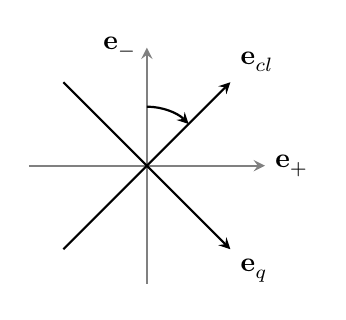
\begin{tikzpicture}[scale=.5,>=stealth]\draw[->,gray,thick](-3,0)--(3,0)node[right,black]{$\vb{e}^{}_+$};\draw[->,gray,thick](0,-3)--(0,3) node[left,black]{$\vb{e}^{}_-$};\begin{scope}[rotate=-45]\draw[->,thick](-3,0)--(3,0)node[below right]{$\vb{e}^{}_q$};\draw[->,thick](0,-3)--(0,3)node[above right]{$\vb{e}^{}_{cl}$};\end{scope}\draw[->,thick](0,1.5)arc(90:45:1.5);\end{tikzpicture}\captionof{figure}{坐标系的旋转,这里令反向支$\vb{e}^{}_-$转到对角线。}\label{fdkgok=-=099056789sfdlgld//.njm}\end{center}
%按照一般的习惯,记对应的\textsl{Keldysh}矢量分量为$\bm{\psi}^K=\psi^{}_q\vb{e}^{}_q+\psi^{}_{cl}\vb{e}^{}_{cl}$,令$\psi^{}_q$为第一个分量,则我们得到
%\begin{equation}\mqty(\psi^{}_{q}\\ \psi^{}_{cl})=\vb{Q}^T\mqty(\psi^{}_+\\ \psi^{}_-)\implies \psi^{}_{cl}=\frac{1}{\sqrt{2}}\qty(\psi^{}_++\psi^{}_-),\quad\psi^{}_{q}=\frac{1}{\sqrt{2}}\qty(\psi^{}_+-\psi^{}_-).\label{haRT455++64sFFG}\end{equation}
%于是我们计算\textsl{Keldysh}张量的变换
%$$\vb{D}=\vb{Q}^{-1}\vb{C}^K\vb{Q}=\frac{1}{2}\mqty(C^{++}+C^{--}-C^{+-}-C^{-+}&C^{+-}+C^{++}-C^{-+}-C^{--}\\ C^{-+}-C^{--}+C^{++}-C^{+-}&C^{++}+C^{+-}+C^{--}+C^{-+}).$$
%按照前文中引入的三个热\textsl{Green}函数(\ref{wuH[]//Ohyugi].,/;'}),我们不难根据\textsl{Keldysh}归一化识别出每一项:$D^{11}=0$,$D^{12}=2\qty(C^{++}-C^{-+})=2D^{}_A$是超前\textsl{Green}函数,$D^{21}=2\qty(C^{++}-C^{+-})=2D^{}_R$是推迟\textsl{Green}函数,$D^{22}=2\qty(C^{++}+C^{--})=2D^{}_S$是\textsl{Schwinger}传播子。于是我们总结得到变换结果为
%\begin{equation}\vb{D}=\mqty(0&D^{}_A\\D^{}_R&D^{}_S).\end{equation}
%我们看到其迹为$\tr(\vb{D})=D^{}_S=\tr(\vb{C}^K)$不变,符合共轭类的定义。因此在\textsl{Keldysh}旋转下,系统自然的从\textsl{Keldysh}张量导出这三个函数,所以只需要计算出$\vb{C}^K$就能完全了解一个热系统的演化。\\
%\\
%最后来看这个旋转的物理含义,方便起见我们省略时空坐标。反解正反分支位形
%$$\mqty(\psi^{}_{+}\\ \psi^{}_{-})=\vb{Q}\mqty(\psi^{}_{q}\\ \psi^{}_{cl})\implies\psi^{}_+=\frac{1}{\sqrt{2}}\qty(\psi^{}_{cl}+\psi^{}_q),\quad\psi^{}_-=\frac{1}{\sqrt{2}}\qty(\psi^{}_{cl}-\psi^{}_q),$$
%则两个\textsl{Wightman}函数写作
%$$C^{-+,+-}=\frac{1}{2}\expval{\qty(\hat{\psi}^{}_{cl}\pm\hat{\psi}^{}_q)\qty(\hat{\psi}^{}_{cl}\mp\hat{\psi}^{}_q)}=\frac{1}{2}\qty(\expval{\hat{\psi}^{}_{cl}\hat{\psi}^{}_{cl}}-\expval{\hat{\psi}^{}_q\hat{\psi}^{}_q}\pm\expval{\comm{\hat{\psi}^{}_{cl}}{\hat{\psi}^{}_q}}).$$
%不难证明对易子的均值为零,因此我们得到
%\begin{equation}C^{-+,+-}=\frac{1}{2}\qty(\expval{\hat{\psi}^{}_{cl}\hat{\psi}^{}_{cl}}-\expval{\hat{\psi}^{}_q\hat{\psi}^{}_q}).\label{][;,;,[]98ud}\end{equation}
%注意这里没有编时或路径乘积。为了计算这两个均值,我们从生成函数(\ref{sgeFCAFC;'p[opk7YT67})出发,在\textsl{Keldysh}旋转下外场同样给出
%$$\vb{J}^K=J^{}_q\vb{e}^{}_q+J^{}_{cl}\vb{e}^{}_{cl},\quad J^{}_{cl}=\frac{1}{\sqrt{2}}\qty(J^{}_++J^{}_-),\quad J^{}_{q}=\frac{1}{\sqrt{2}}\qty(J^{}_+-J^{}_-).$$
%生成函数在形式上是关于外场的,以\textsl{Keldysh}张量为度规的二次型,在正交变换下现在写作
%\begin{equation}\ln(\frac{Z^{}_{SK}\qty(\vb{J}^K;\beta)}{Z^{}_{SK}(0)})=\int \vb{J}^K\vb{D}\vb{J}^K\dd\Omega^2=\int\qty{J^{2}_qD^{11}+J^{}_{cl}J^{}_{q}\qty(D^{12}+D^{21})+J^{2}_{cl}D^{22}}\dd\Omega^2.\end{equation}
%我们知道外场可以通过式(\ref{erTG-*-*-///egb})变为位形,于是在目前的坐标系下,第一个主对角元\textsl{Green}函数给出
%\begin{equation}D^{11}(x,y)=\frac{1}{Z^{}_{SK}(0)}\eval{\qty(\pdv{J^{}_{q}})^2Z^{}_{SK}\qty(\vb{J}^K;\beta)}_{J^{}_q=0}=\expval{\mathbb P\qty{\hat{\psi}^{}_q(x)\hat{\psi}^{}_q(y)}}=0.\label{UGIGYDIOOIIO++--**//+++}\end{equation}
%也就是说,无论处于什么分支,我们都有$\expval{\hat{\psi}^{}_q\hat{\psi}^{}_q}=0$,因而将式(\ref{][;,;,[]98ud})带入\textsl{Wightman}函数的\textsl{SD}方程(\ref{weSRT22--vs})中得到
%\begin{equation}2\hat{\mathcal D}C^{-+,+-}=\hat{\mathcal D}\expval{\hat{\psi}^{}_{cl}\hat{\psi}^{}_{cl}}=0.\end{equation}
%这说明位形$\psi^{}_{cl}$没有接触项,它和满足最小作用量原理的经典场位形是一致的,代表了经典场 \textit{Classical Field}。相反$\psi^{}_q$关于自身的任意\textsl{Green}函数均为零,相较于经典场,这明显确定了量子涨落,因此代表了量子场 \textit{Quantum Field}。可见\textsl{Keldysh}旋转将场分解为经典和量子两部分,其中量子场作为涨落自身没有任何关联性,而经典场确定了系统的动力学性质,其和量子场的耦合确定了关于经典动力学的涨落。这一点在非平衡物理中有根本性的应用。剩下的不难证明有
%\begin{equation}\begin{aligned}D^{22}(x,y)&=\expval{\mathbb P\qty{\hat{\psi}^{}_{cl}(x)\hat{\psi}^{}_{cl}(y)}}=D^{}_S(x,y),\\ D^{12}(x,y)&=\expval{\mathbb P\qty{\hat{\psi}^{}_q(x)\hat{\psi}^{}_{cl}(y)}}=D^{}_A(x,y),\\ D^{21}(x,y)&=\expval{\mathbb P\qty{\hat{\psi}^{}_{cl}(x)\hat{\psi}^{}_q(y)}}=D^{}_R(x,y).\end{aligned}\label{fgHHug++-+659-*-*-*-*++}\end{equation}
%从而我们可以完全的将\textsl{Keldysh}张量用这三个函数,以及$\psi^{}_{\pm}$位形表示,在下面的\textsl{Wick}定理叙述中有重要的作用。
%\subsubsection{SK理论中KG场的多点关联函数}
%\noindent 上面我们详细讨论了时空层面的\textsl{Keldysh}张量,这里我们考虑其在自由\textsl{KG}场中的具体计算及其\textsl{Fourier}分量。我们还会将路径乘积推广至多点关联函数,并讨论相应的\textsl{Wick}定理。\\
%\\
%我们从两个大于和小于函数$C^<$和$C^>$出发,因为它们不涉及编时乘积。记$t=x^0-y^0$,引入占有数算符$\qty{\hat{c}^{}_{\vb{p}},\hat{c}^{\dagger}_{\vb{p}}}$,用能量归一化的自由波函数打开我们得到
%$$\begin{aligned}C^{<}(x,y)=\expval{\hat{\psi}(y)\hat{\psi}(x)}&=\displaystyle\sum_{\vb{p}}\frac{1}{2E^{}_{\vb{p}}}\qty{\expval{\hat{c}^{\dagger}_{\vb{p}}\hat{c}^{}_{\vb{p}}}e^{ip(y-x)}+\expval{\hat{c}^{}_{\vb{p}}\hat{c}^{\dagger}_{\vb{p}}}e^{-ip(y-x)}},\quad t<0,\\ C^{>}(x,y)=\expval{\hat{\psi}(x)\hat{\psi}(y)}&=\displaystyle\sum_{\vb{p}}\frac{1}{2E^{}_{\vb{p}}}\qty{\expval{\hat{c}^{\dagger}_{\vb{p}}\hat{c}^{}_{\vb{p}}}e^{ip(x-y)}+\expval{\hat{c}^{}_{\vb{p}}\hat{c}^{\dagger}_{\vb{p}}}e^{-ip(x-y)}},\quad t>0.\end{aligned}$$
%带入定义$\expval{\hat{c}^{\dagger}_{\vb{p}}\hat{c}^{}_{\vb{p}}}=\expval{n^{}_{\vb{p}}}$,我们得到积分形式
%\begin{equation}\begin{aligned}C^{+-}=C^{<}(x,y)&=\displaystyle\bigintsss\frac{1}{2E^{}_{\vb{p}}}\qty{\expval{n^{}_{\vb{p}}}e^{ip(y-x)}+\qty(\expval{n^{}_{\vb{p}}}+1)e^{-ip(y-x)}}\qty(\frac{\dd p}{2\pi})^3,\quad t<0,\\ C^{-+}=C^{>}(x,y)&=\displaystyle\bigintsss\frac{1}{2E^{}_{\vb{p}}}\qty{\expval{n^{}_{\vb{p}}}e^{ip(x-y)}+\qty(\expval{n^{}_{\vb{p}}}+1)e^{-ip(x-y)}}\qty(\frac{\dd p}{2\pi})^3,\quad t>0.\end{aligned}\end{equation}
%在零温场和平衡热场中,这两个函数都是作为编时乘积的一部分,配合$\theta$函数计算的,实际上我们并没有单独计算过,但现在我们需要得到它们的具体结果。\\
%\\
%这里先计算$C^>$,记坐标差值$x-y=(t,\vb{r})$,采用第\ref{Dee))//}节的思路,将时空分离给出
%$$C^>(t,\vb{r})=\displaystyle\bigintsss\frac{1}{2E^{}_{\vb{p}}}\qty{\expval{n^{}_{\vb{p}}}e^{i\qty(E^{}_{\vb{p}}t-\vb{p}\cdot\vb{r})}+\qty(\expval{n^{}_{\vb{p}}}+1)e^{-i\qty(E^{}_{\vb{p}}t-\vb{p}\cdot\vb{r})}}\qty(\frac{\dd p}{2\pi})^3,\quad t>0.$$
%同样的在积分中做替换$\vb{p}\rightarrow-\vb{p}$积分不变,因此上式可以写为
%\begin{equation}C^>(t,\vb{r})=\displaystyle\bigintsss\frac{1}{2E^{}_{\vb{p}}}e^{i\vb{p}\cdot\vb{r}}\qty{\expval{n^{}_{\vb{p}}}\qty(e^{iE^{}_{\vb{p}}t}+e^{-iE^{}_{\vb{p}}t})+e^{-iE^{}_{\vb{p}}t}}\qty(\frac{\dd p}{2\pi})^3,\quad t>0.\label{Nbd35---59659F}\end{equation}
%为了得到关于四维动量的积分,我们考虑将时间相位用$\delta$函数的\textsl{Fourier}变换表示
%$$\exp(\pm iE^{}_{\vb{p}}t)=2\pi\int \exp(-i\omega t)\delta\qty(\omega\pm E^{}_{\vb{p}})\frac{\dd\omega}{2\pi}.$$
%鉴于\textsl{Green}函数涉及求和$e^{iE^{}_{\vb{p}}t}+e^{-iE^{}_{\vb{p}}t}$,所以这里我们要计算$\delta\qty(\omega+E^{}_{\vb{p}})+\delta\qty(\omega-E^{}_{\vb{p}})$。使用$\delta$函数的性质
%\begin{equation}\delta\qty(a^2-b^2)=\frac{1}{2\abs{a}}\qty{\delta(a-b)+\delta(a+b)},\quad \forall a,b\in\mathbb R,\end{equation}
%两个相位的求和给出
%\begin{equation}\frac{1}{2E^{}_{\vb{p}}}\qty(e^{iE^{}_{\vb{p}}t}+e^{-iE^{}_{\vb{p}}t})=2\pi\int\delta\qty(\omega^2-E^2_{\vb{p}})\frac{\dd\omega}{2\pi}.\end{equation}
%单个相位我们可以利用\textsl{Heaviside}函数$\theta$从中提取特定的$\delta$函数
%$$\frac{1}{2E^{}_{\vb{p}}}e^{-iE^{}_{\vb{p}}t}=2\pi\int\exp(-i\omega t)\theta\qty(E^{}_{\vb{p}})\delta\qty(\omega^2-E^2_{\vb{p}})\frac{\dd\omega}{2\pi}.$$
%因此式(\ref{Nbd35---59659F})可以写作
%\begin{equation}C^>(t,\vb{r})=2\pi\displaystyle\bigintsss e^{i(\vb{p}\cdot\vb{r}-\omega t)}\qty{\expval{n^{}_{\vb{p}}}+\theta\qty(E^{}_{\vb{p}})}\delta\qty(E^{2}_{\vb{p}}-\omega^2)\frac{\dd\omega\dd^3\vb{p}}{(2\pi)^4},\quad t>0.\end{equation}
%因此我们得到相应的动量表象式
%\begin{equation}C^>(\omega,\vb{p})=2\pi\qty{\expval{n^{}_{\vb{p}}}+\theta\qty(E^{}_{\vb{p}})}\delta\qty(\omega^2-E^2_{\vb{p}}).\end{equation}
%类似的计算$C^<$,采用前文的思路写出
%$$C^<(t,\vb{r})=\displaystyle\bigintsss\frac{1}{2E^{}_{\vb{p}}}e^{i\vb{p}\cdot\vb{r}}\qty{\expval{n^{}_{\vb{p}}}\qty(e^{iE^{}_{\vb{p}}t}+e^{-iE^{}_{\vb{p}}t})+e^{iE^{}_{\vb{p}}t}}\qty(\frac{\dd p}{2\pi})^3,\quad t<0.$$
%从而根据上述$\delta$函数的性质,我们得到相应的动量表象式
%\begin{equation}C^<(\omega,\vb{p})=2\pi\qty{\expval{n^{}_{\vb{p}}}+\theta\qty(-E^{}_{\vb{p}})}\delta\qty(\omega^2-E^2_{\vb{p}}).\end{equation}
%对能量带入相对论性色散律$E^{}_{\vb{p}}=p^0=\sqrt{\vb{p}^2+m^2}$得到
%$$\omega^2-E^2_{\vb{p}}=\omega^2-p^2_0=\omega^2-\vb{p}^2-m^2=p^2-m^2,\quad p=(\omega,\vb{p}),$$
%于是在四维动量表象中我们有
%\begin{equation}C^<(p)=2\pi\qty{\expval{n\qty(p^0)}+\theta\qty(-p^0)}\delta\qty(p^2-m^2),\quad C^>(p)=2\pi\qty{\expval{n\qty(p^0)}+\theta\qty(p^0)}\delta\qty(p^2-m^2).\end{equation}
%如果我们将$\mathcal P^{}_2$的微虚$i\epsilon$算上,则可以证明\textsl{Wightman}函数为
%\begin{equation}C^{-+}(p)=\exp(\epsilon p^0)C^>(p),\quad C^{+-}(p)=\exp(-\epsilon p^0)C^>(p).\end{equation}
%因为在处理\textsl{CTP}时我们定义$\epsilon\to\infty$,所以\textsl{Wightman}函数和大于小于函数相等,但是也有其他的选择,比如$\epsilon=\beta/2$,在此规范下可以得到$C^{-+}(p)=C^{+-}(p)$。这个内容就不展开计算了,可以参考\cite{eC..25a}。\\
%\\
%现在来计算两个对角元,不失一般性的还是考虑\textsl{KG}场。我们直接展开编时乘积,每个部分用\textsl{Wightman}函数表示
%$$C^{++}(t,\vb{r})=C^<(t,\vb{r})\theta(-t)+C^>(t,\vb{r})\theta(t),\quad C^{--}(t,\vb{r})=C^<(t,\vb{r})\theta(t)+C^>(t,\vb{r})\theta(-t).$$
%具体打开并考虑到动量反演下积分不变,比如对于正向支$C^{++}$我们得到
%$$C^{++}(t,\vb{r})=\bigintsss\qty(\frac{\dd p}{2\pi})^3e^{i\vb{p}\cdot\vb{r}}\qty{\frac{e^{-iE^{}_{\vb{p}}t}\theta(t)+e^{iE^{}_{\vb{p}}t}\theta(-t)}{2E^{}_{\vb{p}}}+\frac{\expval{n\qty(\omega^{}_{\vb{p}})}\qty(e^{iE^{}_{\vb{p}}t}+e^{-iE^{}_{\vb{p}}t})}{2E^{}_{\vb{p}}}}.$$
%这里我们已经带入了$\theta(-t)+\theta(t)=1$。最终结果和平衡态式(\ref{a/-gfHEDCFeg})必然不同,因为在平衡态中是以离散的\textsl{Matsubara}频率的求和呈现,而此处我们处于四维时空。第一项给出\textsl{Feynman}传播子$D^{}_F$,第二项带入前文中的结论$\delta\qty(p^2-m^2)$,我们得到
%\begin{equation}C^{++}(t,\vb{r})=\bigintsss\qty(\frac{\dd p}{2\pi})^4e^{i(\vb{p}\cdot\vb{r}-\omega t)}\qty{D^{}_F(p)+2\pi\expval{n\qty(p^0)}\delta\qty(p^2-m^2)},\end{equation}
%从而四维动量表象分量为
%\begin{equation}C^{++}(p)=\frac{i}{p^2-m^2+i\epsilon}+2\pi\expval{n\qty(p^0)}\delta\qty(p^2-m^2).\end{equation}
%类似的,我们得到反向支的分量
%\begin{equation}C^{--}(p)=-\frac{i}{p^2-m^2-i\epsilon}+2\pi\expval{n\qty(p^0)}\delta\qty(p^2-m^2).\end{equation}
%注意两个函数微虚的符号相反,这是由于反向支由$e^{-iE^{}_{\vb{p}}t}\theta(-t)+e^{iE^{}_{\vb{p}}t}\theta(t)$控制,用\textsl{Feynman}方法自然得到$-i\epsilon$。不难证明,在这种情况下两者的关系为
%\begin{equation}C^{--}(p)=\qty(C^{++}(p))^*,\end{equation}
%这当然可以从复标量位形的时空\textsl{Green}函数得到,具体请参考\cite{Ld3k} \S92,这里就不展示了。注意到\textsl{Green}函数并非在整个复平面解析,因为涉及到$\delta$函数,\textsl{Wightman}函数也是一样的。因此\textsl{Keldysh}张量不能直接通过\textsl{Matsubara}函数解析延拓得到,这是很合理的,我们从\textsl{CTP}的推导中就已经能看到。\\
%\\
%现在我们不妨计算式(\ref{wuH[]//Ohyugi].,/;'})的三个函数的动量表象,根据定义可以直接从现有结论中得到
%\begin{equation}\begin{aligned}D^{}_R(p)&=C^{++}(p)-C^{+-}(p)=\frac{i}{p^2-m^2+i\epsilon}-2\pi\theta\qty(p^0)\delta\qty(p^2-m^2);\\ D^{}_A(p)&=C^{++}(p)-C^{-+}(p)=\frac{i}{p^2-m^2-i\epsilon}-2\pi\theta\qty(-p^0)\delta\qty(p^2-m^2);\\D^{}_S(p)&=C^{++}(p)+C^{--}(p)=2\pi\qty[1+2\expval{n\qty(p^0)}]\delta\qty(p^2-m^2).\end{aligned}\end{equation}
%注意到$D^{}_R(p)$和$D^{}_A(p)$和温度无关,因为不包含占有数,这是由于它们定义为玻色场的对易子,而玻色对易性和温度无关。同时还可以证明,根据解析性分析得到
%$$\Im D^{}_R(p)=\Im C^{++}(p)=C^<(p)+C^>(p),$$
%这一点在后续的耗散理论中非常重要,目前不做详细解释,只是简单带过。对于这三个函数的具体计算,我们就不展开了,读者可自行验证。\\
%\\
%我们现在要解决的问题,就是\textsl{SK}理论中的热\textsl{Wick}定理。但是不难想到,这一定会比零温场,以及热平衡场更加复杂,因为一个位形可以有两种状态选择。以实标量场的四点函数为例,在路径排序下写作
%\begin{equation}D(1,2,3,4)=\expval{\mathbb P\qty{\hat{\psi}^{}_1\hat{\psi}^{}_2\hat{\psi}^{}_3\hat{\psi}^{}_4}}.\end{equation}
%如果我们打开,考虑到每个位形可以分为$\psi^{}_{\pm}$两个,则上式一共有$2^4=16$种配置,同时还要注意路径排序的约束:正向支算符永远在负向支算符右侧。鉴于正负支算符对易,我们列出几种配置,方便起见记正负支位形为$\hat{\psi}^{\pm}_1=1^{\pm}$
%$$\begin{aligned}&\expval{\mathbb P\qty{1^+2^+3^+4^+}},\quad\expval{\mathbb P\qty{1^-2^+3^+4^+}},\quad\expval{\mathbb P\qty{2^-1^+3^+4^+}},\\&\expval{\mathbb P\qty{1^-4^-2^+3^+}},\quad\expval{\mathbb P\qty{1^-2^-3^-4^-}},\quad\cdots\cdots.\end{aligned}$$
%若按照生成函数计算,则这$16$个配置构成一个二维四阶张量,在张量积表示下其构成一个四维矩阵。这里我们不全部计算,只挑选几个代表性的分量具体说明,其余的只需按照算法做推广即可。先计算全正分支,根据定义(\ref{itGjjF0O--98})我们得到
%\begin{equation}D^{++++}(1,2,3,4)=\expval{\mathbb T\qty{1^+2^+3^+4^+}}.\end{equation}
%这在形式上和通常的零温四点函数一致,为了计算我们可以参考平衡态的\textsl{BdD}定理(\ref{C.deDonmins}),引入关于非平衡热态的正规序$\mathcal N^K$,则我们得到热\textsl{Wick}定理
%\begin{equation}D^{++++}(1,2,3,4)=\expval{\mathcal N^K\qty{1^+2^+3^+4^++\text{所有可能的缩并}}}=C^{++}_{12}C^{++}_{34}+C^{++}_{13}C^{++}_{24}+C^{++}_{23}C^{++}_{14}.\end{equation}
%也就是说,非平衡态的热\textsl{Wick}定理对于正向支,和\textsl{BdD}定理是完全一致的,具体计算过程可以参考平衡态\textsl{Matsubara}频率求和,占有数的统计分布是作为$\mathcal N^K$在以零温正规序定义下的补偿出现的。相应的我们计算反向支
%\begin{equation}D^{----}(1,2,3,4)=\expval{\tilde{\mathbb T}\qty{1^-2^-3^-4^-}}=\expval{\tilde{\mathcal N}^K\qty{1^-2^-3^-4^-+\text{所有可能的缩并}}},\end{equation}
%其中$\tilde{\mathcal N}^K$是反向支上的正规序,和正向支类似我们得到
%\begin{equation}D^{----}(1,2,3,4)=C^{--}_{12}C^{--}_{34}+C^{--}_{13}C^{--}_{24}+C^{--}_{23}C^{--}_{14}.\end{equation}
%也就是说在同一分支上,多点函数的热\textsl{Wick}定理和\textsl{BdD}定理是完全一致的,我们只需要按照零温\textsl{Wick}定理打开编时乘积,再对\textsl{Gree}函数带入\textsl{Keyldsh}矩阵对角元即可。\\
%\\
%当然在实际应用中,更加重要的混合分量,因为这是平衡态和零温场无法描述的。从单个反向支出发,我们写出
%\begin{equation}D^{-+++}(1,2,3,4)=\expval{\mathbb P\qty{1^-2^+3^+4^+}}\end{equation}
%基于$\mathcal P^{}_1$和$\mathcal P^{}_2$两个分支上算符的独立性,我们对路径排序做这样的处理:反向支上的算符$\hat{\psi}^-_1$可以从路径排序中提出,剩下三个在正向支上的算符取时序乘积,在上述热\textsl{Wick}定理下写作
%\begin{equation}D^{-+++}(1,2,3,4)=\expval{1^-\circ\mathbb T\qty{2^+3^+4^+}}=\expval{1^-\circ\mathcal N\qty{2^+3^+4^++\text{所有可能的缩并}}}.\end{equation}
%将所有可能的缩并展开
%$$1^-\circ\mathbb T\qty{2^+3^+4^+}=1^-\circ\mathcal N^K\qty{2^+3^+4^++\wick{\c{2}\vphantom{2}^+\c{3}\vphantom{3}^+4^+}+\wick{\c{2}\vphantom{2}^+3^+\c{4}\vphantom{4}^+} +\wick{2^+\c{3}\vphantom{3}^+\c{4}\vphantom{4}^+}},$$
%此时在正规序外剩下一个落单的$\hat{\psi}^-_1$,按照复合映射$\circ$的分配律确定缩并
%\begin{equation}1^-\circ\mathbb T\qty{2^+3^+4^+}\equiv\mathcal N^K\qty{1^-2^+3^+4^+}+\wick{\c2{1}\vphantom{1}^-\c1{2}\vphantom{2}^+\c1{3}\vphantom{3}^+\c2{4}\vphantom{4}^+}+\wick{\c2{1}\vphantom{1}^-\c1{2}\vphantom{2}^+\c2{3}\vphantom{3}^+\c1{4}\vphantom{4}^+}+\wick{\c1{1}\vphantom{1}^-\c1{2}\vphantom{2}^+\c2{3}\vphantom{3}^+\c2{4}\vphantom{4}^+}.\end{equation}
%将大于\textsl{Green}函数定义为混合缩并
%\begin{equation}C^>_{12}=C^{-+}_{12}=\wick{\c{1}\vphantom{1}^-\c{2}\vphantom{2}^+}=\expval{\wick{\c{1}\vphantom{1}^-\c{2}\vphantom{2}^+}}\in\mathbb C,\end{equation}
%我们得到包含单个反向支的四点函数
%\begin{equation}D^{-+++}(1,2,3,4)=C^{-+}_{12}C^{++}_{34}+C^{-+}_{13}C^{++}_{24}+C^{-+}_{14}C^{++}_{23}.\end{equation}
%这里一定要注意变量的顺序,再次强调反向支$1^-$要在左侧,也就是$1$一定是在其余数字的左边。类似的我们可以推广至单个反向支在最后一个位形的情况,比如
%\begin{equation}D^{-+++}(4,1,2,3)=\expval{\mathbb P\qty{1^+2^+3^+4^-}}.\end{equation}
%按照上面的定义我们展开,将$\hat{\psi}^-_4$提出再和反向正规序缩并
%$$\mathbb P\qty{1^+2^+3^+4^-}=4^-\circ\mathbb T\qty{1^+2^+3^+}=\mathcal N^K\qty{4^-1^+2^+3^+}+\wick{\c1{4}\vphantom{4}^-\c1{1}\vphantom{1}^+\c2{2}\vphantom{2}^+\c2{3}\vphantom{3}^+}+\wick{\c2{4}\vphantom{4}^-\c1{1}\vphantom{1}^+\c2{2}\vphantom{2}^+\c1{3}\vphantom{3}^+}+\wick{\c2{4}\vphantom{4}^-\c1{1}\vphantom{1}^+\c1{2}\vphantom{2}^+\c2{3}\vphantom{3}^+},$$
%定义相应的缩并为小于\textsl{Green}函数
%\begin{equation}C^<_{12}=C^{+-}_{12}=\wick{\c{2}\vphantom{2}^-\c{1}\vphantom{1}^+}=\expval{\wick{\c{2}\vphantom{2}^-\c{1}\vphantom{1}^+}}\in\mathbb C,\end{equation}
%我们得到结论
%\begin{equation}D^{-+++}(4,1,2,3)=C^{++}_{23}C^{+-}_{14}+C^{++}_{13}C^{+-}_{24}+C^{++}_{12}C^{+-}_{34}.\end{equation}
%注意此时$4$是在右侧,因为按照零温场表述,时间$t^{}_4$应该是最小的,但现在其是最大的,按照原排序依旧记在右边,自然其对应负号也处于右侧,时间差和通常的理解相反对应小于\textsl{Green}函数。类似的读者可以自行计算单个正向支的情况,这里不做展开。\\
%\\
%但是上述的操作在每个分支包含多个算符的时候会失效,比如对于四点函数我们计算
%\begin{equation}D^{--++}(1,2,3,4)=\expval{\mathbb P\qty{1^-2^-3^+4^+}}=\expval{\tilde{\mathbb T}\qty{1^-2^-}\mathbb T\qty{3^+4^+}}.\end{equation}
%第二个等号是绝对成立的,这由分支上算符的独立性保证。若按照上述分支单算符的推导,我们按照对应的正规序写出热\textsl{Wick}定理
%$$\tilde{\mathbb T}\qty{1^-2^-}\mathbb T\qty{3^+4^+}=\tilde{\mathcal N}^K\qty{1^-2^-+\wick{\c{1}\vphantom{1}^-\c{2}\vphantom{2}^-}}\circ\mathcal N^K\qty{3^+4^++\wick{\c{3}\vphantom{3}^+\c{4}\vphantom{4}^+}}.$$
%如果我们直接使用分配律,则结果为
%$$\tilde{\mathbb T}\qty{1^-2^-}\mathbb T\qty{3^+4^+}=\tilde{\mathcal N}^K\qty{1^-2^-}\circ\mathcal N^K\qty{3^+4^+}+C^{++}_{34}\tilde{\mathcal N}^K\qty{1^-2^-}+C^{--}_{12}\mathcal N^K\qty{3^+4^+}+C^{--}_{12}C^{++}_{34}.$$
%这里我们已经将缩并用\textsl{Green}函数表示了。但是参照\textsl{BdD}定理,热正规序满足$\expval{\mathcal N^K\qty{\cdots}}=0$,反向也一样,这意味着最终的结果是
%$$!!\quad D^{--++}(1,2,3,4)=C^{--}_{12}C^{++}_{34}.\quad!!$$
%这明显是不合理的,因为若我们写出其对应的生成函数表述
%\begin{equation}D^{--++}(1,2,3,4)=\frac{1}{Z^{}_{SK}(0;\beta)}\eval{\pdv{J^-_1}\pdv{J^-_2}\pdv{J^+_3}\pdv{J^+_4}Z^{}_{SK}\qty(\vb{J}^K;\beta)}_{\vb{J}^K=0},\end{equation}
%带入\textsl{SK}泛函(\ref{sgeFCAFC;'p[opk7YT67})打开得到
%$$\begin{aligned}&D^{--++}(1,2,3,4)=\eval{\pdv{J^-_1}\pdv{J^-_2}\pdv{J^+_3}\pdv{J^+_4}\exp{\int \qty(\vb{J}^K)^T\vb{C}\qty(\vb{J}^K)\dd\Omega^2}}_{\vb{J}^K=0}\\&=\eval{\pdv{J^-_1}\pdv{J^-_2}\pdv{J^+_3}\int\qty(C^{++}_{4y}J^+_y+C^{+-}_{4y}J^-_y)\dd\Omega^{}_y\exp{\int\qty(\vb{J}^K)^T\vb{C}\qty(\vb{J}^K)\dd\Omega^2}}_{\vb{J}^K=0}\\&=\cdots\cdots\\&=C^{++}_{43}C^{--}_{21}+C^{+-}_{42}C^{+-}_{31}+C^{+-}_{32}C^{+-}_{41}=\wick{\c2{4}\vphantom{4}^+\c2{3}\vphantom{3}^+\c1{2}\vphantom{2}^-\c1{1}\vphantom{1}^+}+\wick{\c2{4}\vphantom{4}^+\c1{3}\vphantom{3}^+\c2{2}\vphantom{2}^-\c1{1}\vphantom{1}^+}+\wick{\c2{4}\vphantom{4}^+\c1{3}\vphantom{3}^+\c1{2}\vphantom{2}^-\c2{1}\vphantom{1}^+}.\end{aligned}$$
%具体的计算细节就不展示了,请读者自行补全,这里对于四个\textsl{Wightman}函数,根据式(\ref{g++FSG-++++hfs})可知变量的顺序并没有影响,只需要同时对换符号即可。这说明此四点函数最终的结构,仍然表述为单正规序内所有可能的缩并,单对缩并的均值为零,最终的结论和零温以及平衡热场的\textsl{Wick}定理完全一致。\\
%\\
%这个事实说明,我们需要一种能同时处理两个分支算符的方法,用以得到正确的结果。回顾到\textsl{Keldysh}旋转,根据定义(\ref{haRT455++64sFFG})我们将正负支的位形变为经典和量子两个部分,且式(\ref{fgHHug++-+659-*-*-*-*++})说明\textsl{Keldysh}张量可以用这两个新的量确定。因此我们不妨尝试$\psi^{}_{cl,q}$表述,方便起见记$\hat{\psi}^{cl}_{1}\qty(x^{}_1)=1^{}_{cl}$,根据定义我们有
%$$1^+=\frac{1}{\sqrt{2}}\qty(1^{}_{cl}+1^{}_q),\quad 1^-=\frac{1}{\sqrt{2}}\qty(1^{}_{cl}-1^{}_q),$$
%带入路径排序得到
%$$\begin{aligned}\mathbb P\qty{1^-2^-3^+4^+}&=\qty(\frac{1}{\sqrt{2}})^4\mathbb P\qty{\qty(1^{}_{cl}-1^{}_q)\qty(2^{}_{cl}-2^{}_q)\qty(3^{}_{cl}+3^{}_q)\qty(4^{}_{cl}+4^{}_q)}\\&=\frac{1}{4}\mathbb P\qty{\qty(1^{}_{cl}2^{}_{cl}-1^{}_q2^{}_{cl}-1^{}_{cl}2^{}_q+1^{}_q2^{}_q)\qty(3^{}_{cl}4^{}_{cl}-3^{}_q4^{}_{cl}-3^{}_{cl}4^{}_q+3^{}_q4^{}_q)}.\end{aligned}$$
%注意这里的数字是算符,因此不能随意对换位置。根据式(\ref{UGIGYDIOOIIO++--**//+++})我们知道量子场没有关联函数,这里写作$\expval{\mathbb P\qty{1^{}_q2^{}_q}}=0$,所以上式在取均值后,所有包含多量子场乘积的项均消失,只剩下五项
%$$\frac{1}{4}\expval{\mathbb P\qty{\qty(1^{}_{cl}2^{}_{cl})\qty(3^{}_{cl}4^{}_{cl})-\qty(1^{}_{cl}2^{}_{cl})\qty(3^{}_q4^{}_{cl})-\qty(1^{}_{cl}2^{}_{cl})\qty(3^{}_{cl}4^{}_q)-\qty(1^{}_q2^{}_{cl})\qty(3^{}_{cl}4^{}_{cl})-\qty(1^{}_{cl}2^{}_q)\qty(3^{}_{cl}4^{}_{cl})}}.$$
%注意这里的括号不能忽略。利用式(\ref{fgHHug++-+659-*-*-*-*++}),将上式各括号内的乘积用$D^S$,$D^A$和$D^R$表示四点函数
%\begin{equation}D^{--++}(1,2,3,4)=\frac{1}{4}\qty(D^S_{12}D^S_{34}-D^S_{12}D^A_{34}-D^S_{12}D^R_{34}-D^A_{12}D^S_{34}-D^R_{12}D^S_{34}).\end{equation}
%再根据定义式(\ref{wuH[]//Ohyugi].,/;'})回到$\vb{C}$形式的\textsl{Keldysh}张量,我们就得到热\textsl{Wick}定理
%\begin{equation}D^{--++}(1,2,3,4)=\expval{\tilde{\mathbb T}\qty{1^-2^-}\mathbb T\qty{3^+4^+}}=C^{--}_{12}C^{++}_{34}+C^{-+}_{13}C^{-+}_{24}+C^{-+}_{23}C^{-+}_{14}.\end{equation}
%这意味着,我们其实完全可以只定义一个关于路径排序的正规序$\mathcal N^P$,满足\textsl{BdD}定理
%\begin{equation}\mathcal N^P\qty(\hat{c}\hat{c}^{\dagger})=\hat{c}^{\dagger}\hat{c},\quad\mathcal N^P\qty(\hat{b}\hat{c}^\dagger\hat{c})=\hat{c}^\dagger\hat{b}\hat{c},\quad\expval{\mathcal N^P\qty{\hat{\psi}^{\pm}_1\hat{\psi}^{\pm}_2\hat{\psi}^{\pm}_3\cdots}}=0.\end{equation}
%从而\textsl{SK}形式中的热\textsl{Wick}定理就表述为
%\begin{equation}D(1,2,\ldots)=\expval{\mathbb P\qty{\hat{\psi}^{\pm}_1\hat{\psi}^{\pm}_2\cdots}}=\expval{\mathcal N^P\qty{\hat{\psi}^{\pm}_1\hat{\psi}^{\pm}_2\cdots+\text{所有可能的缩并}}}.\end{equation}
%这样我们就将前文中分支单算符的情况也归纳了进来,相应的缩并这里用\textsl{Keldysh}矩阵总结为
%\begin{equation}\vb{C}^K(1,2)=\mqty(C^{++}_{12}&C^{+-}_{12}\\C^{-+}_{12}&C^{--}_{12})=\mqty(\wick[offset=1.2em]{\c{\hat{\psi}}\vphantom{\hat{\psi}}^+_1\c{\hat{\psi}}\vphantom{\hat{\psi}}^+_2}&\wick[offset=1.2em]{\c{\hat{\psi}}\vphantom{\hat{\psi}}^+_1\c{\hat{\psi}}\vphantom{\hat{\psi}}^-_2}\\ \wick[offset=1.2em]{\c{\hat{\psi}}\vphantom{\hat{\psi}}^-_1\c{\hat{\psi}}\vphantom{\hat{\psi}}^+_2}&\wick[offset=1.2em]{\c{\hat{\psi}}\vphantom{\hat{\psi}}^-_1\c{\hat{\psi}}\vphantom{\hat{\psi}}^-_2}).\end{equation}
%并且我们可以轻松的推广至任意多点函数,总体结构和零温场依旧保持一致。这实际上是\textsl{Wick}定理的宏观普遍性质,具体说明可以参考九卷\cite{L2} \S13的结尾部分,因此无论系统的性质如何,其依旧是以所有可能的缩并体现在统计中。\clearpage
%\section{量子微扰论}\label{DFVO))//}
%\noindent 在之前的叙述中,我们不止一次的提及“微扰”这个概念,比如电磁波是电磁场的微扰,相变中外场对系统的微扰等。一般来讲在物理上,\textbf{微扰 \textit{Pertubation}}指的是系统的已知演化在小增量下的变化,通常用于求解复杂系统的演化方程。比如已知系统参量$y$的演化方程为$\hat{\mathcal{D}}^{}_0y^{}_0=h^{}_0$,小增量定义为
%$$\hat{\mathcal{D}}(\epsilon)=\sum_{n=0}\epsilon^n\hat{\mathcal{D}}^{}_n,\quad h=\sum_{n=0}\epsilon^nh^{}_n,\quad \epsilon\sim o(1),$$
%从而总参量解写为$y=\sum\limits_{n=0}\epsilon^ny^{}_n$,带入方程$\hat{\mathcal{D}}y=h$便能得到关于$\epsilon$的幂级数关系。我们称阶为$n$的级数为\textbf{n级微扰},相应阶数的解为\textbf{n级近似 \textit{n$^{\text{th}}$Approximation}},对应的项$y^{}_n$为\textbf{n级修正 \textit{n$^{\text{th}}$Correction}}。事实上前文中的各阶展开就是相应的近似,具体的应用已有大量涉及,请读者自行查看。\\
%\\
%关于经典力学中的微扰论,在附录\ref{Y6TY.,.,''}中会以奇异摄动论具体展开,这里就略过了。下文中我们具体研究量子体系中的微扰问题,关于其群论解释这里也略过。
%\subsection{经典定态微扰}\label{DFVO)2)//}
%\noindent 我们从\textbf{定态微扰 \textit{Static Pertubation}}开始。假设系统的已知态由零级近似$\hat{H}^{}_0$确定,其定态\textsl{Schrödinger}方程为
%\begin{equation}\hat{H}^{}_0\psi^{(0)}=E^{(0)}\psi^{(0)},\end{equation}
%于是系统的一级微扰$\sim\epsilon$可以表示为
%\begin{equation}\hat{H}\psi=\qty(\hat{H}^{}_0+\epsilon\hat{V})\psi=E\psi.\label{shouaxian}\end{equation}
%由于能量是离散且有限的,所以上述问题在算符的矩阵元下可以化为二阶矩阵本征方程的扰动。为此我们先从通常的矩阵出发分析,再通过\textsl{Hilbert}空间回到量子系统。
%\subsubsection{矩阵的自本征微扰}
%方便起见这里讨论向量空间$\mathbb V$上的实对称矩阵$\vb{A}^{}_{ab}$,记其谱为$\text{Sp}\qty(\vb{A},\mathbb V)=\qty{\lambda^{(0)}_i}$,其扰动$\vb{B}^{}_{ab}$给出
%\begin{equation}\vb{A}^{}_{ab}\vb{e}^{(i)a}=\lambda^{(0)}_i\vb{e}^{(i)}_b,\quad\qty(\vb{A}^{}_{ab}+\epsilon\vb{B}^{}_{ab})\vb{f}^{(i)a}=\lambda^{}_i\vb{f}^{(i)}_b.\label{.,.,.,><>jh}\end{equation}
%我们将新主值也记为$\lambda$,\underline{是为了使得在$\epsilon=0$时仍为$\vb{A}^{}_{ab}$的本征方程*},对于不同记号情况的讨论参考下文。因为矩阵的加法要求两个矩阵的性质相同,也就是处于同一个向量空间$\mathbb V$中,所以新的本征向量$\vb{f}^{(i)}$也可以对单位正交基$\qty{\vb{e}^{(i)}}$分解
%\begin{equation}\vb{f}^{(i)}=\sum_jc^{}_{ij}\vb{e}^{(j)},\quad c^{}_{ij}\neq0\in\mathbb R.\label{awrgtfse}\end{equation}
%于是本征方程的扰动就可以解释为:由基变换诱导的矩阵变换。我们将上述分解带入式(\ref{.,.,.,><>jh})中,并带入$\vb{A}^{}_{ab}$的本征方程得到
%$$\qty(\vb{A}^{}_{ab}+\epsilon\vb{B}^{}_{ab})\sum_jc^{}_{ij}\vb{e}^{(j)a}=\sum_jc^{}_{ij}\qty(\lambda^{(0)}_j\vb{e}^{(j)}_b+\epsilon\vb{B}^{}_{ab}\vb{e}^{(j)a})=\lambda^{}_i\sum_jc^{}_{ij}\vb{e}^{(j)}_b.$$
%由于$\vb{B}^{}_{ab}\vb{e}^{(j)a}$不是以基$\vb{e}^{(j)}_b$表示的,所以我们利用正交性写出分量式。引入微扰矩阵关于主值号$\{i\in\mathbb N\}$的矩阵元
%\begin{equation}B^{ij}=B^{ji}=B^{}_{ij}=\vb{B}^{}_{ab}\vb{e}^{(j)a}\vb{e}^{(i)b}=\vb{B}\qty(\vb{e}^{(i)},\vb{e}^{(j)}),\label{w4,.,><>jh}\end{equation}
%则在两边同乘$\vb{e}^{(k)b}$,且正交性给出$\vb{e}^{(i)a}\vb{e}^{(j)}_{b}=\delta^{ij}\delta^a_b$,我们得到新旧主值之间的关系
%\begin{equation}\qty(\lambda^{}_i-\lambda^{(0)}_k)c^{}_{ik}=\sum_j\epsilon c^{}_{ij}B^{}_{jk}.\label{str11r}\end{equation}
%根据经典微扰理论,我们将变换系数和新主值的解写为$\epsilon$的幂级数形式,注意新本征值根据定义在零级近似下等于$\lambda^{(0)}_i$
%$$c^{}_{ij}=\sum_{\alpha=0}\epsilon^\alpha c^{(\alpha)}_{ij},\quad\lambda^{}_i=\sum_{\alpha=0}\epsilon^\alpha \lambda^{(\alpha)}_i,\ \qty(\epsilon=0\implies\alpha=1,\lambda^{}_i\equiv\lambda^{(0)}_i)$$
%其中变换系数级数展开由本征向量定义为
%$$\vb{f}^{(i)}=\sum_{\alpha=0}\vb{f}^{(i);\alpha}=\sum_{\alpha=0}\sum_j\epsilon^\alpha c^{(\alpha)}_{ij}\vb{e}^{(j)}.$$
%将级数带入关系式(\ref{str11r}),注意求和记号的更改给出
%\begin{equation}\qty(\sum_{\alpha=0}\epsilon^\alpha \lambda^{(\alpha)}_i-\lambda^{(0)}_k)\sum_{\alpha=0}\epsilon^\alpha c^{(\alpha)}_{ik}=\sum_{\beta=0}\sum_j\epsilon^{\beta+1}c^{(\beta)}_{ij}B^{}_{jk}.\end{equation}
%现在我们来列举解的若干级的近似方程,通过两侧$\epsilon$幂级数的系数相等得到:
%\begin{enumerate}\item[\quad0.] 零级近似:$\epsilon^0=1\Longleftrightarrow\alpha=\beta+1=0$,相应的系数为\begin{equation}\qty(\lambda^{(0)}_i-\lambda^{(0)}_k)c^{(0)}_{ik}=0.\label{nmdo1}\end{equation}可以看到这是微扰本征方程(\ref{.,.,.,><>jh})在$\epsilon=0$时的情况。\item 一级近似:$\epsilon^1\Longleftrightarrow\alpha=\beta+1=1$,相应的系数为$$\qty(\lambda^{(0)}_i+\epsilon\lambda^{(1)}_i-\lambda^{(0)}_k)\qty(c^{(0)}_{ik}+\epsilon c^{(1)}_{ik})=\sum_j\epsilon c^{(0)}_{ij}B^{}_{jk},$$我们从中提出$\sim\epsilon$的系数给出 \begin{equation}\qty(\lambda^{(0)}_i-\lambda^{(0)}_k)c^{(1)}_{ik}=\sum_jc^{(0)}_{ij}B^{}_{jk}-\lambda^{(1)}_ic^{(0)}_{ik}.\label{nmdo2}\end{equation}当然上式也可以带入方程(\ref{nmdo1})得到,相当于消去了零级近似。\item 二级近似:$\epsilon^2\Longleftrightarrow\alpha=\beta+1=2$,相应的系数为$$\qty(\lambda^{(0)}_i+\epsilon\lambda^{(1)}_i+\epsilon^2\lambda^{(2)}_i-\lambda^{(0)}_k)\qty(c^{(0)}_{ik}+\epsilon c^{(1)}_{ik}+\epsilon^2 c^{(2)}_{ik})=\sum_j\epsilon\qty(c^{(0)}_{ij}+\epsilon c^{(1)}_{ij})B^{}_{jk},$$类似的我们得到方程 \begin{equation}\qty(\lambda^{(0)}_i-\lambda^{(0)}_k)c^{(2)}_{ik}+\lambda^{(2)}_ic^{(0)}_{ik}=\sum_jc^{(1)}_{ij}B^{}_{jk}-\lambda^{(1)}_ic^{(1)}_{ik}.\label{nmdo3}\end{equation}同样的带入前面两个方程就能得到,不再赘述。\item 其余高阶近似就不一一列举了,读者可自行带入$\epsilon=1$得到相应的系数关系。 \end{enumerate}
%上述方程组便是矩阵微扰论的基础,它们确定了各级近似之间的递推关系。而方程(\ref{nmdo1})立马确定了两种不同的情况:$\lambda^{(0)}_i\neq\lambda^{(0)}_k$和$\lambda^{(0)}_i=\lambda^{(0)}_k$,两者对应了不同的变换系数。这实际上就是谱$\text{Sp}\qty(\vb{A},\mathbb V)$是否有重根,其代数理论可以通过主值分析得到。这里我们分别来讨论这两种情形。\\
%\\
%对于非重根的情况,我们有$\forall i\neq k,\quad\lambda^{(0)}_i\neq\lambda^{(0)}_k$。根据主值分析,单位正交基$\qty{\vb{e}^{(i)}}$是自然存在的,前面的讨论均完整适用。此时方程(\ref{nmdo1})一个自然的根为$c^{(0)}_{ik}=0$,当然因为系数不可能为零,所以我们可以令
%$$c^{(0)}_{ik}=u\delta^{}_{ik},\quad u\in \mathbb R,$$
%则方程变为$\qty(\lambda^{(0)}_i-\lambda^{(0)}_k)\delta^{}_{ik}\equiv0$恒成立。带入方程(\ref{nmdo2})得到
%$$\qty(\lambda^{(0)}_i-\lambda^{(0)}_k)c^{(1)}_{ik}=u\qty(\delta^{j}_{i}B^{}_{jk}-\lambda^{(1)}_i\delta^{}_{ik})=u\qty(B^{}_{ik}-\lambda^{(1)}_i\delta^{}_{ik}).$$
%注意到当$i=k$时上式恒为零$\lambda^{(0)}_i-\lambda^{(0)}_i\equiv0$,于是我们得到本征值的一级修正为
%\begin{equation}\lambda^{(1)}_i=B^{}_{ii}=\vb{B}^{}_{ab}\vb{e}^{(i)a}\vb{e}^{(i)b}.\end{equation}
%也就是说谱的一级修正为一级微扰的对角元,这是合理的,因为此时两个本征向量共线$\vb{f}^{(i);0}=u\vb{e}^{(i)}$。由此也可以证明,若在微扰方程中记新本征值为$\kappa^{}_i$,则我们必然有$u\kappa^{(0)}_i=\lambda^{(0)}_i$。将其归一化后我们得到$u=1$,也就是在零级近似下$\vb{f}^{(i);0}=\vb{e}^{(i)}$且$\kappa^{(0)}_i=\lambda^{(0)}_i$,\underline{这符合我们的预设*},则方程(\ref{nmdo2})给出系数和本征向量的一级修正为
%\begin{equation}c^{(1)}_{ik}=\eval{\frac{B^{}_{ik}}{\lambda^{(0)}_i-\lambda^{(0)}_k}}_{i\neq k},\quad \vb{f}^{(i);1}_a=\sum_kc^{(1)}_{ik}\vb{e}^{(k)}_a=\sum_{k\neq i}\frac{B^{}_{ik}\vb{e}^{(k)}_a}{\lambda^{(0)}_i-\lambda^{(0)}_k}.\label{bukene8}\end{equation}
%由此我们可以看到微扰的约束条件:在量级上$\vb{f}^{(i);1}_a\sim\epsilon\vb{f}^{(i);0}_a=\epsilon\vb{e}^{(k)}_a$,所以上式给出
%\begin{equation}\epsilon\sim\frac{B^{}_{ik}}{\lambda^{(0)}_i-\lambda^{(0)}_k}\ll1\implies \abs{B^{}_{ik}}\ll\abs{\lambda^{(0)}_i-\lambda^{(0)}_k}.\end{equation}
%这就是说,微扰矩阵元要远小于两个旧本征值之差,否则精度会有极大偏差。并且我们还可以直接求得关于主值号$\{i\}$的矩阵元的近似,类似式(\ref{w4,.,><>jh})引入记号
%$$G^{}_{ij}=\qty(\vb{A}^{}_{ab}+\epsilon\vb{B}^{}_{ab})\vb{f}^{(i)a}\vb{f}^{(j)b}=\sum_{\alpha=0}\epsilon^{\alpha}G^{(\alpha)}_{ij},\quad G^{(0)}_{ij}=\vb{A}^{}_{ab}\vb{e}^{(i)a}\vb{e}^{(j)b},$$
%则一级修正给出
%\begin{equation}G^{(1)}_{ij}=\sum_{k\neq i}\frac{B^{}_{ik}G^{(0)}_{kj}}{\lambda^{(0)}_i-\lambda^{(0)}_k}+\sum_{k\neq j}\frac{B^{}_{jk}G^{(0)}_{ki}}{\lambda^{(0)}_j-\lambda^{(0)}_k}.\label{LACHI}\end{equation}
%类似的我们来求二级近似,将上面所得结果都带入方程(\ref{nmdo3})中得到
%$$\qty(\lambda^{(0)}_i-\lambda^{(0)}_k)c^{(2)}_{ik}=\sum_j\qty(B^{}_{jk}-B^{}_{ii})\eval{\frac{B^{}_{ij}}{\lambda^{(0)}_i-\lambda^{(0)}_j}}_{i\neq j}-\lambda^{(2)}_k,$$
%同样令$i=k$得到本征值的二级修正为
%\begin{equation}\lambda^{(2)}_i=\sum_{j\neq i}\frac{\abs{B^{}_{ij}}^2}{\lambda^{(0)}_i-\lambda^{(0)}_j}.\label{wanqqi0)}\end{equation}
%相应的可以求出本征向量的二级修正,在归一化$\expval{\vb{f}^{(i);2},\vb{f}^{(i);2}}=1$后得到
%\begin{equation}\vb{f}^{(i);2}=\sum_{j\neq i}\sum_{k\neq i}\frac{B^{}_{jk}B^{}_{ki}}{\omega^{}_{ik}\omega^{}_{ij}}\vb{e}^{(j)}-\sum_{j\neq i}\frac{B^{}_{ii}B^{}_{ji}}{\omega^2_{ij}}\vb{e}^{(j)}-\frac{1}{2}\vb{e}^{(i)}\sum_{j\neq i}\frac{\abs{B^{}_{ji}}^2}{\omega^2_{ij}},\quad \omega^{}_{ij}=\lambda^{(0)}_i-\lambda^{(0)}_j.\label{shuaillo}\end{equation}
%再给出本征值的三级修正
%\begin{equation}\lambda^{(3)}_i=\sum_{j\neq i}\sum_{k\neq i}\frac{B^{}_{ij}B^{}_{jk}B^{}_{ki}}{\omega^{}_{ik}\omega^{}_{ij}}-B^{}_{ii}\sum_{j\neq i}\frac{\abs{B^{}_{ji}}^2}{\omega^2_{ij}}.\end{equation}
%上述两式请读者自行验证,关于更高阶的近似也略过,此处不再具体展开。\\
%\\
%对于重根$\lambda^{(0)}_i=\lambda^{(0)}_k$的情况,结论会略微复杂一些,我们先讨论一级近似。此时单位正交基$\qty{\vb{e}^{(i)}_a}$并非自然存在,而是需要通过\textsl{Schmidt}正交化定理构造。设重根的重数为$s$,相应的子向量空间和单位基记为
%$$\mathbb V^{}_{(0)}=\text{Span}\qty{\vb{e}^{(\xi)}\middle\vert 1\leq \xi\leq s}\subset \mathbb V,$$
%于是在$u=1$下本征向量的零级近似给出单位正交基
%\begin{equation}\vb{f}^{();0}=\sum_\xi c^{(0)}_{\xi}\vb{e}^{(\xi)},\quad c^{(0)}_{\xi}\neq0.\end{equation}
%这里我们不预先指出该本征向量对应的本征值号,因为无法确定这是否依旧是重根。此时近似方程组依旧成立,但是需要做一定的修改。对于微扰矩阵,式(\ref{w4,.,><>jh})在空间$\mathbb V^{}_{(0)}$下应定义为
%$$B^{\xi\eta}=B^{\eta\xi}=B^{}_{\xi\eta}=\vb{B}^{}_{ab}\vb{e}^{(\xi)a}\vb{e}^{(\eta)b}=\vb{B}\qty(\vb{e}^{(\xi)},\vb{e}^{(\eta)}).$$
%对于一级近似方程(\ref{nmdo2}),重根导致其恒为零,做类似的正交操作并按照上述指标写为
%\begin{equation}\sum_{\xi=1}^s B^{}_{\xi\eta}c^{(0)}_{\xi}-\lambda^{(1)}c^{(0)}_{\eta}=0 \Longleftrightarrow \sum_{\xi=1}^s\qty(B^{}_{\xi\eta}-\lambda^{(1)}\delta^{}_{\xi\eta})c^{(0)}_{\xi}=0,\quad1\leq \eta\leq s.\label{Lofee}\end{equation}
%这是一个以$\vb{c}^{(0)}=\qty(c^{(0)}_{\xi})$为变量向量的齐次线性方程组,其非零解满足代数方程 (也称为\textbf{久期方程})
%\begin{equation}\abs{B^{}_{\xi\eta}-\lambda^{(1)}\delta^{}_{\xi\eta}}=0,\quad1\leq \xi,\eta\leq s.\end{equation}
%我们看到,重根的一级近似在其空间$\mathbb V^{}_{(0)}$下构成了微扰矩阵$\vb{B}^{}_{ab}$的谱
%\begin{equation}\text{Sp}\qty(\vb{B}^{}_{ab},\mathbb V^{}_{(0)})=\qty{\lambda^{(1)}_{\kappa}\big\vert1\leq \kappa\leq s}.\label{fenlle8}\end{equation}
%一般而言矩阵主值的重根数$s>1$,也就是说$\exists \kappa^{}_1\neq\kappa^{}_2$,使得$\lambda^{(1)}_{\kappa^{}_1}\neq\lambda^{(1)}_{\kappa^{}_2}$。这样一来零级近似下的重根在微扰下分裂为若干个值,且本征向量的零级近似由$B^{}_{\xi\eta}$的本征向量确定,总的来说能确定$s$个向量$\in \mathbb V^{}_{(0)}$,并构成一组新的单位正交基。\\
%\\
%但这里需要强调一点,上述$\vb{B}^{}_{ab}$的对角化操作只在子空间$\mathbb V^{}_{(0)}$中有效,在补空间$\mathbb V^{\complement}_{(0)}$中不成立。事实上这可以通过对比非重根的结论看到,其中一级近似只是$\mathbb V$上的对角元,而并非主值。这说明若系统原来存在若干重复本征值,则$\mathbb V$中包含为相同数目且互不相交的子空间$\mathbb V^{}_{(0)}$,使得微扰在各子空间中对角化,这是空间可约的表现。
%\subsubsection{矩阵的跨本征微扰}
%\noindent 上面我们只讨论了重根自身的分裂,但一级近似还存在另一种来源,即子空间$\mathbb V^{}_{(0)}$和其补空间$\mathbb V^{\complement}_{(0)}$之间的\textbf{交换}。此近似和非重根情况是十分类似的,都是不同主值下的情况,不同点在于此处微扰是跨空间的,所以有必要重新讨论。\\
%\\
%方便起见,我们保持$\mathbb V^{}_{(0)}$的记号不变,记其补空间和相应的谱为
%$$\mathbb V^{\complement}_{(0)}=\mathbb V-\mathbb V^{}_{(0)}=\text{Span}\qty{\vb{e}^{(i)}\middle\vert\vb{e}^{(i)a}\vb{e}^{(\xi)}_a\equiv0},$$
%$$\text{Sp}\qty(\vb{A}^{}_{ab},\mathbb V^{\complement}_{(0)})=\qty{\lambda^{(0)}_i\big\vert\vb{A}^{}_{ab}\vb{e}^{(i)a}=\lambda^{(0)}_i\vb{e}^{(i)}_b},$$
%$\mathbb V^{\complement}_{(0)}$主值号的选择继承自$\mathbb V$,则在直和$\mathbb V=\mathbb V^{}_{(0)}\oplus\mathbb V^{\complement}_{(0)}$的含义下,本征向量的变换定义为
%$$\vb{f}=\sum_jc^{}_{j}\vb{e}^{(j)}+\sum_\xi c^{}_{\xi}\vb{e}^{(\xi)}\in\mathbb V,$$
%若我们考虑其在$\mathbb V^{\complement}_{(0)}$上的限制,按照相应的记号可以写为
%\begin{equation}\vb{f}^{(i)}=\eval{\vb{f}}_{\mathbb V^{\complement}_{(0)}}=\sum_jc^{}_{ij}\vb{e}^{(j)}+\sum_\xi c^{}_{i\xi}\vb{e}^{(\xi)}\in\eval{\mathbb V}_{\mathbb V^{\complement}_{(0)}},\label{cainm65}\end{equation}
%反之在$\mathbb V^{}_{(0)}$上的限制为
%\begin{equation}\vb{f}^{(\eta)}=\eval{\vb{f}}_{\mathbb V^{}_{(0)}}=\sum_jc^{}_{\eta j}\vb{e}^{(j)}+\sum_\xi c^{}_{\xi\eta}\vb{e}^{(\xi)}\in\eval{\mathbb V}_{\mathbb V^{}_{(0)}}.\label{cainm66}\end{equation}
%这里对于向量的限制应该用延拓来理解,而非简单的投影,具体几何语言参考式(\ref{cainm67})。暂时记重根为$\theta^{(0)}_k$并\underline{令其为孤立的},此时补空间对应非重根。取零级近似$\epsilon=0$,并将微扰方程在$\mathbb V^{\complement}_{(0)}$中写出
%$$\eval{\vb{A}(\vb{f})}_{\mathbb V^{\complement}_{(0)}}=\vb{A}^{}_{ab}\vb{f}^{(i)a;0}=\sum_jc^{(0)}_{ij}\lambda^{(0)}_j\vb{e}^{(j)}_b+\sum_\xi\theta^{(0)}_kc^{(0)}_{i\xi}\vb{e}^{(\xi)}_b=\lambda^{(0)}_i\qty(\sum_jc^{(0)}_{ij}\vb{e}^{(j)}_b+\sum_\xi c^{(0)}_{i\xi}\vb{e}^{(\xi)}_b).$$
%对其乘以$\vb{e}^{(\xi)b}$,不难看到零级近似方程(\ref{nmdo1})现在写为
%\begin{equation}\qty(\lambda^{(0)}_i-\theta^{(0)}_k)c^{(0)}_{i\xi}=0,\quad \lambda^{(0)}_i\neq\theta^{(0)}_k.\end{equation}
%于是我们得到$c^{(0)}_{i\xi}\equiv0$,也就是说零级近似下两个空间之间没有基变换,给出$\vb{f}^{(i);0}=\sum\limits_jc^{(0)}_{ij}\vb{e}^{(j)}$,这是由直和性质保证的。同时我们也证明了在$\mathbb V^{}_{(0)}$中$\vb{f}^{(\eta);0}=\sum\limits_\xi c^{(0)}_{\xi\eta}\vb{e}^{(\xi)}$,读者可自行确认。\\
%\\
%对于一级近似$\epsilon=1$,我们写出在两个空间下各自的微扰方程,并不预先指出$\lambda^{(1)}$的主值号
%$$\begin{aligned}\mathbb V^{\complement}_{(0)}:\quad&\qty(\vb{A}^{}_{ab}+\vb{B}^{}_{ab})\vb{f}^{(i)a;1}=\qty(\lambda^{(0)}_i+\lambda^{(1)})\vb{f}^{(i);1}_b\\&=\sum_j\qty(c^{(0)}_{ij}+c^{(1)}_{ij})\qty(\lambda^{(0)}_j\vb{e}^{(j)}_b+\vb{B}^{}_{ab}\vb{e}^{(j)a})+\sum_\xi\qty(c^{(0)}_{i\xi}+c^{(1)}_{i\xi})\qty(\theta^{(0)}_k\vb{e}^{(\xi)}_b+\vb{B}^{}_{ab}\vb{e}^{(\xi)a})\\&=\qty(\lambda^{(0)}_i+\lambda^{(1)})\qty{\sum_j\qty(c^{(0)}_{ij}+c^{(1)}_{ij})\vb{e}^{(j)}_b+\sum_\xi\qty(c^{(0)}_{i\xi}+c^{(1)}_{i\xi})\vb{e}^{(\xi)}_b}.\end{aligned}$$
%$$\begin{aligned}\mathbb V^{}_{(0)}:\quad&\qty(\vb{A}^{}_{ab}+\vb{B}^{}_{ab})\vb{f}^{(\eta)a;1}=\qty(\theta^{(0)}_k+\lambda^{(1)})\vb{f}^{(\eta);1}_b\\&=\sum_j\qty(c^{(0)}_{\eta j}+c^{(1)}_{\eta j})\qty(\lambda^{(0)}_j\vb{e}^{(j)}_b+\vb{B}^{}_{ab}\vb{e}^{(j)a})+\sum_\xi\qty(c^{(0)}_{\eta\xi}+c^{(1)}_{\eta\xi})\qty(\theta^{(0)}_k\vb{e}^{(\xi)}_b+\vb{B}^{}_{ab}\vb{e}^{(\xi)a})\\&=\qty(\theta^{(0)}_k+\lambda^{(1)})\qty{\sum_j\qty(c^{(0)}_{\eta j}+c^{(1)}_{\eta j})\vb{e}^{(j)}_b+\sum_\xi\qty(c^{(0)}_{\eta\xi}+c^{(1)}_{\eta\xi})\vb{e}^{(\xi)}_b}.\end{aligned}$$
%类似的引入跨空间微扰矩阵元
%\begin{equation}B^{i\xi}=B^{}_{i\xi}=\vb{B}^{}_{ab}\vb{e}^{(i)a}\vb{e}^{(\xi)b},\end{equation}
%对两个方程分别乘上基$\vb{e}^{(\delta)b}$和$\vb{e}^{(l)b}$,减去零级近似,并带入前面的结论$c^{(0)}_{i\xi}\equiv0$后我们得到四个一级近似方程
%\begin{enumerate}[\quad(1)]\item$\quad\sum\limits_jc^{(0)}_{ij}B^{}_{jl}+c^{(1)}_{il}\lambda^{(0)}_l=\lambda^{(0)}_ic^{(1)}_{il}+\lambda^{(1)}c^{(0)}_{il};$\item$\quad\sum\limits_jc^{(0)}_{ij}B^{}_{j\delta}+c^{(1)}_{i\delta}\theta^{(0)}_k=\lambda^{(0)}_ic^{(1)}_{i\delta};$\item$\quad c^{(1)}_{\eta l}\lambda^{(0)}_l+\sum\limits_\xi c^{(0)}_{\eta\xi}B^{}_{l\xi}=\theta^{(0)}_kc^{(1)}_{\eta l};$\item$\quad\sum\limits_\xi c^{(0)}_{\eta\xi}B^{}_{\xi\delta}+c^{(1)}_{\eta\delta}\theta^{(0)}_k+\qty(\sum\limits_jc^{(1)}_{\eta j}B^{}_{j\delta})^*=\theta^{(0)}_kc^{(1)}_{\eta\delta}+\lambda^{(1)}c^{(0)}_{\eta\delta}.$ \end{enumerate}
%其中我们对方程$(4)$增加了一个二级项$\sim c^{(1)}\vb{B}^{}_{ab}$,因为一级项的重根抵消了。\\
%\\
%现在我们具体分析,当然此时方程(\ref{Lofee})不再适用 (所处空间不完整),通过方程$(3)$解得
%\begin{equation}c^{(1)}_{\eta i}=\sum\limits_\xi\frac{B^{}_{i\xi}}{\theta^{(0)}_k-\lambda^{(0)}_i}c^{(0)}_{\eta\xi},\quad\theta^{(0)}_k\neq\lambda^{(0)}_i. \end{equation}
%又因为之前解出$c^{(0)}_{ij}=\delta^{}_{ij}$,并且鉴于$\theta^{(0)}_k$的孤立性导致$\lambda^{(0)}_i\neq\lambda^{(0)}_l$,于是从方程$(1)$和$(2)$得到
%$$\lambda^{(1)}=B^{}_{ii},\quad c^{(1)}_{i\neq j}=\frac{B^{}_{ij}}{\lambda^{(0)}_i-\lambda^{(0)}_j},\quad c^{(1)}_{i\delta}=\frac{B^{}_{i\delta}}{\lambda^{(0)}_i-\theta^{(0)}_k}.$$
%其中前两式就是非重根情况下的一级修正,而第三式则是对系数$c^{(1)}_{\eta i}$在$\mathbb V^{\complement}_{(0)}$上的修正,因此我们得到跨空间变换系数的一级修正
%\begin{equation}c^{(1)}_{i\eta}=\frac{B^{}_{i\eta}}{\lambda^{(0)}_i-\theta^{(0)}_k}+\sum\limits_\xi\frac{B^{}_{i\xi}}{\theta^{(0)}_k-\lambda^{(0)}_i}c^{(0)}_{\eta\xi}.\label{wsgdsb}\end{equation}
%需要强调,重根$\theta^{(0)}_k$不参与求和,因为它是常数。对于方程$(4)$,我们带入上面的系数得到
%$$\lambda^{(1)}c^{(0)}_{\eta\delta}=\sum\limits_\xi c^{(0)}_{\eta\xi}B^{}_{\xi\delta}+\sum\limits_j\frac{B^{}_{j\eta}B^{}_{j\delta}}{\lambda^{(0)}_i-\theta^{(0)}_k}+\sum\limits_j\sum\limits_\xi\frac{B^{}_{j\xi}B^{}_{j\delta}}{\theta^{(0)}_k-\lambda^{(0)}_i}c^{(0)}_{\eta\xi}.$$
%要注意由于带入的是二级项,因而其中的常数项在量级上给出
%$$\sum\limits_j\frac{B^{}_{j\eta}B^{}_{j\delta}}{\lambda^{(0)}_i-\theta^{(0)}_k}=(const)^{}_{\eta\xi}\ll\sum\limits_j\sum\limits_\xi\frac{B^{}_{j\xi}B^{}_{j\delta}}{\theta^{(0)}_k-\lambda^{(0)}_i}c^{(0)}_{\eta\xi},$$
%所以这一项在方程中可以省略。类似前文,我们省略指标$\eta$后将方程写为本征形式
%\begin{equation}\lambda^{(1)}c^{(0)}_{\delta}=\sum\limits_\xi c^{(0)}_{\xi}\qty(B^{}_{\xi\delta}+\sum\limits_j\frac{B^{}_{j\xi}B^{}_{j\delta}}{\theta^{(0)}_k-\lambda^{(0)}_i}).\end{equation}
%对比方程(\ref{Lofee})我们看到,久期方程中的常数项应做替换
%$$B^{}_{\xi\delta}\rightarrow B'_{\xi\delta}=B^{}_{\xi\delta}+\sum\limits_j\frac{B^{}_{j\xi}B^{}_{j\delta}}{\theta^{(0)}_k-\lambda^{(0)}_i}\implies\abs{B^{}_{\xi\eta}+\sum\limits_j\frac{B^{}_{j\xi}B^{}_{j\delta}}{\theta^{(0)}_k-\lambda^{(0)}_i}-\lambda^{(1)}\delta^{}_{\xi\eta}}=0.$$
%由此解得一级修正$\lambda^{(1)}$为$B'_{\xi\delta}$的谱,微扰矩阵元精确到二级,它和式(\ref{fenlle8})所确定的分裂是不同的。并且系数$c^{(0)}_{\xi}$也有一定的修正,这主要是由于补空间对微扰的贡献导致的。相应的我们写出本征向量的一级近似,方便起见设$\epsilon=1$,注意跨空间的一级修正由公式确定(\ref{wsgdsb}),此处以$\mathbb V^{\complement}_{(0)}$为例
%\begin{equation}\begin{aligned}\vb{f}^{(i)}&=\sum_j\qty(c^{(0)}_{ij}+c^{(1)}_{ij})\vb{e}^{(j)}+\epsilon\sum_\eta c^{(1)}_{i\eta}\vb{e}^{(\eta)}\\&=\vb{e}^{(i)}+\sum_{j\neq i}\frac{B^{}_{ij}\vb{e}^{(j)}}{\lambda^{(0)}_i-\lambda^{(0)}_j}+\sum_\eta\qty(\frac{B^{}_{i\eta}}{\lambda^{(0)}_i-\theta^{(0)}_k}+\sum\limits_\xi\frac{B^{}_{i\xi}c^{(0)}_{\eta\xi}}{\theta^{(0)}_k-\lambda^{(0)}_i})\vb{e}^{(\eta)}.\end{aligned}\end{equation}
%对于$\mathbb V^{}_{(0)}$中的向量请读者自行写出。最后还是强调一下,上面我们所讨论的内容只限于孤立重根,若原本征值$\text{Sp}\qty(\vb{A},\mathbb V)$有若干重根,则在每个子空间$\mathbb V^{}_{(0)}$中取一级近似后,不仅需要和补空间实行上述操作,还应互相实行同样的操作,当然子空间之间互不相交。这里的补空间是针对所有子空间的,从而保证它依旧确定非重根近似,我们就不做展开了。\\
%\\
%对于二级近似,从上述代数讨论中不难看到,对于孤立重根$\theta^{(0)}_k$而言有五种可能性。虽然一级近似分裂了零级重根,但是其作为主值仍有存在重根的可能性,这也就意味着子空间$\mathbb V^{}_{(0)}$依旧是可约的。设此一级近似重根$\theta^{(1)}_k$为孤立的,则一种简单的来源是$\theta^{(1)}_k$的分裂,但需要注意此时二级近似本质是子空间$\mathbb V^{}_{(0)}$上的一级近似,所以不适用方程(\ref{nmdo3})。我们记其子空间为
%$$\mathbb V^{}_{(1)}=\text{Span}\qty{\vb{f}^{(\varpi);0}\middle\vert 1\leq\varpi\leq d}\subset \mathbb V^{}_{(0)},$$
%引入其上的微扰矩阵元
%$$B^{}_{\varpi\vartheta}=\vb{B}^{}_{ab}\vb{f}^{(\varpi)a;0}\vb{e}^{(\vartheta)b;0},$$
%则其上方程(\ref{nmdo2})给出二级近似递推
%\begin{equation}\sum_{\varpi=1}^d B^{}_{\varpi\vartheta}c^{(1)}_{\varpi}-\lambda^{(2)}c^{(1)}_{\vartheta}=0 \Longleftrightarrow \abs{B^{}_{\varpi\vartheta}-\lambda^{(2)}\delta^{}_{\varpi\vartheta}}=0,\quad1\leq\vartheta\leq d.\end{equation}
%同样的解出久期方程,得到$\vb{B}^{}_{ab}$关于子空间$\mathbb V^{}_{(1)}$的谱,从而解除一级近似下的重根。记$\mathbb V^{}_{(1)}$关于$\mathbb V^{}_{(0)}$的补空间为
%$$\complement_{\mathbb V^{}_{(0)}}\mathbb V^{}_{(1)}=\text{Span}\qty{\vb{e}^{(\xi)}}\subset \mathbb V^{}_{(0)},$$
%则另一种简单的来源就是由$\complement_{\mathbb V^{}_{(0)}}\mathbb V^{}_{(1)}$确定的非重根情况,上述定义保证了非重根空间的主值号直接继承自其母空间。此时我们只需要重复非重根部分的操作即可,采用$\mathbb V^{}_{(0)}$的记号我们直接给出相应的结果:
%\begin{equation}c^{(1)}_{i\xi}=\frac{B^{}_{i\xi}}{\theta^{(0)}_k-\lambda^{(0)}_j},\quad c^{(1)}_{\eta\xi}=\frac{1}{B^{}_{\xi\xi}-B^{}_{\eta\eta}}\sum_j\frac{B^{}_{\eta j}B^{}_{j\xi}}{\theta^{(0)}_k-\lambda^{(0)}_j},\quad\lambda^{(2)}_i=\sum_\xi \frac{\abs{B_{i\xi}}^2}{\theta^{(0)}_k-\lambda^{(0)}_i}.\end{equation}
%注意到本征值的二级修正和式(\ref{wanqqi0)})在形式上是类似的,这可以由方程(\ref{nmdo3})确定,并且我们得到本征向量在$\mathbb V^{}_{(0)}$上的一级修正
%\begin{equation}\vb{f}^{(i);1}=\sum_\xi c^{(1)}_{i\xi}\vb{e}^{(\xi)},\quad \vb{f}^{(\eta);1}=\sum_\xi c^{(1)}_{\eta\xi}\vb{e}^{(\xi)}.\end{equation}
%强调一下,由于这里是直接的非重根解,因此不需要取直和的叠加,采用$\mathbb V^{}_{(0)}$上的普遍公式(\ref{awrgtfse})即可。当然这只是二级近似的部分值,剩下的三种是:
%\begin{itemize}\item$\mathbb V^{}_{(1)}$和$\mathbb V^{\complement}_{(0)}$之间的交换,确定了二级分裂后由原非重根导致的修正;
%\item $\complement_{\mathbb V^{}_{(0)}}\mathbb V^{}_{(1)}$和$\mathbb V^{}_{(1)}$的交换,确定了二级分裂后由一级分裂的非重根导致的修正;
%\item $\complement_{\mathbb V^{}_{(0)}}\mathbb V^{}_{(1)}$和$\mathbb V^{\complement}_{(0)}$之间的交换,确定了二级分裂后两个额外修正之间的变换。\end{itemize}
%一般而言这三种情况是非常小的高级修正,可以忽略不计,所以二级近似主要由一级近似下重根的直接递推和分裂确定。\\
%\\
%以下用向量空间之间的关联总结上述内容,这里我们仅考虑各级重根均为孤立的,且忽略交换导致的高级修正:
%\begin{center}\tikz{[node distance=.1cm and 2cm]\node(A){$\mathbb V$};\node(B)[below right=of A]{$\mathbb V^{}_{(0)}$};\node(C)[above right=of A]{$\mathbb V^{\complement}_{(0)}$};\node(D)[right=of A]{$\oplus$};\node(E)[below right=of B]{$\mathbb V^{}_{(1)}$};\node(F)[above right=of B]{$\complement_{\mathbb V^{}_{(0)}}\mathbb V^{}_{(1)}$};\node(G)[right=of B]{$\oplus$};\node(H)[below right=of E]{$\mathbb V^{}_{(2)}$};\node(I)[above right=of E]{$\complement_{\mathbb V^{}_{(1)}}\mathbb V^{}_{(2)}$};\node(J)[right=of E]{$\oplus$};\foreach\parent/\child in{A/B,B/E,E/H}\draw(\parent)--node[below,sloped,pos=0.5]{\scriptsize 孤立重根分裂}(\child);\foreach\parent/\child in{A/C,B/F,E/I}\draw(\parent)--node[above,sloped,pos=0.5]{\scriptsize 非重根}(\child);\foreach\parent/\child in{B/C,E/F,H/I}\draw(\parent)--node[right,pos=0.5]{\scriptsize 交换}(\child);\node(K)[right=of J]{$\cdots\cdots$};\node(L)[right=of C]{$\mathbb V^{\complement}_{(0)}$};\node(M)[right=of F]{$\complement_{\mathbb V^{}_{(0)}}\mathbb V^{}_{(1)}$};\draw(C)--(L);\draw(F)--(M);}\captionof{figure}{微扰导致的向量空间分裂示意图,此处近似到二阶}\label{as223}\end{center}
%其中从左到右各级近似从零级开始,相同向量空间直连代表无重根下的情况,其中近似级数为向量空间指标加一。请读者自行给出多重根的关联图,比如可以追踪本征向量的基看到。\\
%\\
%关于微扰的几何解释参见附录\ref{ha324ong},这里我们就略过了。当然值得指出的是,上面的思路同样可用于浸渐分析,且会涉及大量的纤维丛理论,和微扰论如出一辙,感兴趣的读者请参考\cite{L6f}。
%\subsubsection{量子定态微扰的矩阵表述}
%\noindent 现在我们将矩阵的微扰应用于量子体系中,来讨论量子系统的定态微扰。首先量子算符都是\textsl{Hermitian},这保证了其矩阵元都是复对称的,其次根据方程(\ref{shouaxian})可知,向量就是波函数,本征值就是能量,此时系统处于能量表象。同时本征值的重复就是能量的简并,因此微扰对重根的分裂就是解除简并。\\
%\\
%由方程(\ref{shouaxian})我们将微扰写为$\hat{H}^{}_1=\vb{B}$,微扰前后的本征向量为$\vb{e}^{(i)a}=\ket{i^{(0)}},\vb{f}^{(i)a}=\ket{i}$,于是我们很容易的就能从前面的结论写出系统的微扰理论:
%\begin{itemize}\item 非简并情况:能量$E^{}_i=\lambda^{}_i$的一级修正为\begin{equation}E^{(1)}_i=B^{}_{ii}=\mel**{i^{(0)}}{\hat{V}}{i^{(0)}}=\int\psi^{(0)*}_i(x)\hat{V}\psi^{(0)}_i(x)\dd x.\end{equation}波函数的一级修正为\begin{equation}\ket{i^{(1)}}=\vb{f}^{(i);1}=\sum_{k\neq i}\frac{B^{}_{ik}}{E^{(0)}_i-E^{(0)}_k}\ket{k^{(0)}},\quad B^{}_{ik}=\mel**{i^{(0)}}{\hat{V}}{k^{(0)}}.\end{equation}能量的二级修正为\begin{equation}E^{(2)}_i=\sum_{j\neq i}\frac{B^{}_{ij}B^{}_{ji}}{E^{(0)}_i-E^{(0)}_j}=\sum_{j\neq i}\frac{\abs{B^{}_{ij}}^2}{E^{(0)}_i-E^{(0)}_j}.\end{equation}注意此处$B^{}_{ij}B^{}_{ji}=\abs{B^{}_{ij}}^2$是由于其\textsl{Hermitian},读者可自行验证。其余内容我们就不再重复写出了。\item 简并情况:简并能量$E^{}_k=\lambda^{}_i$的一级修正满足久期方程\begin{equation}\abs{B^{}_{\xi\eta}-E^{(1)}\delta^{}_{\xi\eta}}=0,\quad B^{}_{\xi\eta}=\mel**{\xi^{(0)}}{\hat{V}}{\eta^{(0)}}.\end{equation}其中$\qty{\ket{\xi^{(0)}}}$是围绕前的简并波函数,微扰后的零级近似$$\qty{\ket{k^{(0)}}}=\sum_\eta c^{(0)}_{\eta}\ket{\eta^{(0)}}$$构成一组单位正交基,其叠加系数$c^{(0)}_{\eta}$是$B^{}_{\xi\eta}$的本征向量。后续的简并情况也按照类似的方法处理即可,不再赘述。\item 交换情况:设简并能量为$E^{}_k$,对于简并波函数的处理如上,则能量的一级修正满足\begin{equation}E^{(1)}c^{(0)}_{\delta}=\sum\limits_\xi c^{(0)}_{\xi}\qty(B^{}_{\xi\delta}+\sum\limits_j\frac{B^{}_{j\xi}B^{}_{j\delta}}{E^{(0)}_k-E^{(0)}_i}),\quad B^{}_{i\xi}=\mel**{i^{(0)}}{\hat{V}}{\xi^{(0)}}.\end{equation}可见系统的简并和非简并态在微扰下呈现为混合态,进而在分裂中产生亦一些中间能级。具体的求解和简并情况是类似的。 \end{itemize}
%值得一提的是,由于算符允许连续谱的情况,因此我们也可以考察连续谱的微扰。比如我们假设$\hat{H}^{}_0$存在连续的能量谱,记为$\text{Sp}=\qty{E^{(0)}_\nu\vert\nu\in I\subset\mathbb R^+}$,则关于非简并能级波函数的一级修正为
%\begin{equation}\ket{i^{(1)}}=\sum_{k\neq i}\frac{B^{}_{ik}}{E^{(0)}_i-E^{(0)}_k}\ket{k^{(0)}}+\int\frac{B^{}_{i\nu}}{E^{(0)}_i-E^{(0)}_\nu}\ket{\nu^{(0)}}\dd\nu,\end{equation}
%其中$\ket{\nu^{(0)}}$是连续谱对应的本征向量,$B^{}_{i\nu}$是相应的矩阵元。当然需要注意,虽然我们此处考察连续能量谱非简并,但一般而言连续谱一般而言是简并的,比如动量$\vb{k}$等。因此这里的推广是不完整的,具体参见附录\ref{hqwrgong}。
%
%\subsection{经典含时微扰和演化跃迁}\label{yonghur}
%\noindent 上面我们介绍了定态微扰,但是对于一般的力学系统而言,状态是随着时间而变化的。因而我们更多的是想讨论,在演化过程中一个扰动如何对系统产生影响,这就是量子含时微扰。关于其几何结构,参见附录\ref{hanshiy}。\\
%\\
%我们从完全已知的零级近似开始。令$\hat{H}^{}_0$和时间无关,即系统能量守恒,在能量表象下取单位初始态$\phi^{(0)}$,则含时\textsl{Schrödinger}方程为
%$$i\hbar\dv{t}\psi^{(0)}(t)=\hat{H}^{}_0\psi^{(0)}(t)=E^{(0)}\psi^{(0)}(t),$$
%不难写出解为
%$$\psi^{(0)}(t)=\phi^{(0)}\exp(-\frac{i}{\hbar}E^{(0)}t)=\hat{\tau}(t)\phi^{(0)},$$
%其中$\hat{\tau}(t)$是按式(\ref{cndisf})引入的时间演化算符。参考式(\ref{shouaxian}),我们写出含时的一级微扰为
%\begin{equation}i\hbar\dv{t}\psi(t)=\qty{\hat{H}^{}_0+\epsilon\hat{V}(t)}\psi(t).\end{equation}
%其中,算符对于时间的相关性归结到微扰$\hat{V}(t)$上。不失一般性的,我们依旧先考察矩阵形式,再回到量子系统,讨论时间演化下的态跃迁概率。
%\subsubsection{矩阵含时微扰论}
%\noindent 取向量空间$\mathbb V$上的定值对称矩阵$\vb{A}$,同样的记其谱为$\text{Sp}\qty(\vb{A},\mathbb V)=\qty{\lambda^{(0)}_i}$,因此零级近似写为
%$$\dv{t}\vb{e}^{(i)a}=\vb{A}^{}_{ab}\vb{e}^{(i)a}=\lambda^{(0)}_i\vb{e}^{(i)}_b.$$
%记$\vb{A}$的单位本征向量为$\vb{a}^{(i)}$,使得$\mathbb V=\text{Span}=\qty{\vb{a}^{(i)}}$,则上述解为$\vb{e}^{(i)}(t)=\vb{a}^{(i)}\exp(\lambda^{(0)}_it)$。但由于本征向量是归一化的,因此指数项只可能是复相位,从而方程必须写成
%\begin{equation}i\dv{t}\vb{e}^{(i)a}=\vb{A}^{}_{ab}\vb{e}^{(i)a}=\lambda^{(0)}_i\vb{e}^{(i)}_b,\quad \vb{e}^{(i)a}(t)=\vb{a}^a\exp(-i\lambda^{(0)}_it).\label{zhuyi66}\end{equation}
%并且由于复相位在复空间中体现为旋转,因此我们取
%$$\mathbb V=\mathbb C=\text{Span}\qty{\vb{a}}=\text{Span}\qty{\vb{e}(t)},$$
%也就是向量在演化中依旧构成复空间的一组单位正交基,此时矩阵$\vb{A}$为复\textit{Hermitian}。在复空间上,一级微扰给出
%\begin{equation}i\dv{t}\vb{f}(t)=\qty{\vb{A}+\epsilon\vb{B}(t)}\vb{f}(t),\label{juzhenxc*}\end{equation}
%因为微扰$\vb{B}$和时间有关,所以我们无法继续从本征值的角度考虑,$\vb{f}$也就不一定是本征向量。但是矩阵的加法约束依旧成立,因而我们参考式(\ref{awrgtfse})写出基变换
%\begin{equation}\vb{f}(t)=\sum_jc^{}_{j}(t)\vb{e}^{(j)}(t),\quad c^{}_{j}(t)\in\mathbb C=\text{Span}\qty{\vb{f}(t)},\end{equation}
%注意这里的基变换系数也是时间的函数。代入微扰方程中我们得到
%$$i\dv{t}\vb{f}=i\sum_j\qty(\dv{c^{}_j}{t}\vb{e}^{(j)}+c^{}_j\dv{t}\vb{e}^{(j)})=\sum_jc^{}_j\qty{\lambda^{(0)}_j\vb{e}^{(j)}+\epsilon\vb{B}\qty(\vb{e}^{(j)})(t)}.$$
%注意到零级近似(\ref{zhuyi66}),并对变换系数取幂级数,我们得到
%\begin{equation}i\sum_\alpha\sum_j\epsilon^{(\alpha)}\dv{c^{(\alpha)}_j}{t}\vb{e}^{(j)}=\sum_\beta\epsilon^{(\beta+1)}\sum_jc^{(\beta)}_j\vb{B}\qty(\vb{e}^{(j)})(t).\end{equation}
%不难看到这个方程的特性:右侧的近似要比左侧的高一级,这意味着对于第$n=\alpha$级修正项我们必然有$\beta=n-1$,右侧系数的修正总是比左侧低一级。同时上式对于任意本征值都成立,无论其是否重复,但这并不代表重根不会产生问题。\\
%\\
%现在我们来考察各级近似,不妨从零级修正开始。根据上面的叙述,我们得到$\beta=0-1=-1$,这是不可能的,从而我们得到
%\begin{equation}\sum_j\dv{c^{(0)}_j}{t}\vb{e}^{(j)}=0\implies c^{(0)}_j=const.\end{equation}
%如果我们取$\vb{f}$的零级修正为$\vb{A}$的本征向量$\vb{f}^{(k);0}=\sum\limits_jc^{(0)}_{kj}\vb{e}^{(j)}$,对应本征值$\lambda^{}_k$,则根据定态结论不难看到
%\begin{itemize}\item 非重根$\lambda^{}_j\neq\lambda^{}_k$:本征值对本征向量为双射$\vb{f}^{(k);0}=\vb{e}^{(k)}\implies c^{(0)}_{kj}=c^{(0)}_{jk}=\delta^{}_{kj}$;\item 重根$\lambda^{}_j=\lambda^{}_k$:本征向量构成子空间$\mathbb V^{}_{(0)}$,叠加系数在该空间中是任意的,$c^{(0)}_{kj}\neq\delta^{}_{kj}$。\end{itemize}
%在上述假设下,考察本征向量$\vb{f}^{(k)}$的一级近似方程
%\begin{equation}\epsilon^1: i\sum_j\dv{c^{(1)}_{kj}}{t}\vb{e}^{(j)}=\sum_jc^{(0)}_{kj}\vb{B}\qty(\vb{e}^{(j)})(t),\label{rtgrg4}\end{equation}
%不难看到在非重根情况下,我们有
%$$i\sum_j\dv{c^{(1)}_{kj}}{t}\vb{e}^{(j)}=\sum_j\delta^{}_{kj}\vb{B}\qty(\vb{e}^{(j)})(t)=\vb{B}\qty(\vb{e}^{(k)})(t).$$
%由于$\vb{e}$是复向量,因此这里的内积按式(\ref{nfjt})的定义确定,在前文中已经有过多次涉及,我们将归一化写成$\expval{\vb{e}^{(i)},\vb{e}^{(j)}}=\delta^{ij}$。类似式(\ref{w4,.,><>jh}),同样的引入扰矩阵关于主值号的矩阵元
%\begin{equation}B^{}_{ij}(t)=\vb{B}^{}_{ab}(t)\vb{e}^{(j)a}\vb{e}^{(i)*b}=\vb{B}\qty(\vb{e}^{(i)*},\vb{e}^{(j)}),\end{equation}
%注意这是\textit{Hermitian}矩阵元。代入零级近似解(\ref{zhuyi66}),以及矩阵的双线性性得到
%\begin{equation}B^{}_{ij}(t)=\vb{B}\qty(\vb{a}^{(i)*},\vb{a}^{(j)})(t)\exp(i\lambda^{(0)}_it)\exp(-i\lambda^{(0)}_jt)=b^{}_{ij}(t)\exp{i\qty(\lambda^{(0)}_i-\lambda^{(0)}_j)t},\end{equation}
%其中$b^{}_{ij}(t)=\vb{B}\qty(\vb{a}^{(i)},\vb{a}^{(j)})(t)$是不含相位的矩阵元部分。于是将方程在$\vb{e}^{(l)}$上投影,我们得到
%$$i\sum_j\dv{c^{(1)}_{kj}}{t}\delta^{jl}=i\dv{c^{(1)}_{lk}}{t}=\vb{B}\qty(\vb{e}^{(l)*},\vb{e}^{(k)})(t)=B^{}_{lk}(t),$$
%引入\textbf{\textsl{Bohr}频率}$\omega^{}_{ij}=\lambda^{(0)}_i-\lambda^{(0)}_j$,从而变换系数的一级修正为
%\begin{equation}c^{(1)}_{ij}=-i\int b^{}_{ij}\qty(t')\exp(i\omega^{}_{ij}t')\dd t'.\label{wifsh8}\end{equation}
%于是向量的一级修正就是$\vb{f}^{;1}=\sum\limits_iA^{}_i\vb{f}^{(i);1}=\sum\limits_{ij}A^{}_ic^{(1)}_{ij}\vb{e}^{(j)}$,其中$A^{}_i$是归一化系数。\\
%\\
%重根情况无法直接使用上述结论,因为此时方程(\ref{rtgrg4})无法将各项分离。参考定态微扰,解除重根的方法是将微扰对角化,这里也做类似的操作,考虑到相位的独立性,对角化的对象是$b^{}_{ij}$,记其特征向量为$\bm{\zeta}^{(\vartheta)}$。这样一来子空间写为$\mathbb V^{}_{(0)}=\text{Span}\qty{\bm{\zeta}^{(\vartheta)}}$。将特征向量$\vb{f}^{(\varphi);0}$在子空间$\mathbb V^{}_{(0)}$下展开
%$$\vb{f}^{(\varphi);0}=\sum\limits_\vartheta c^{(0)}_{\varphi\vartheta}\bm{\zeta}^{(\vartheta)}\in\mathbb V^{}_{(0)},\quad \bm{\zeta}^{(\vartheta)}(t)=\bm{\beta}^{(\vartheta)}\exp(-i\lambda^{(0)}_kt),$$
%一级近似方程(\ref{rtgrg4})写作
%$$\epsilon^1: i\sum_\vartheta\dv{c^{(1)}_{\varphi\vartheta}}{t}\bm{\zeta}^{(\vartheta)}=\sum_\vartheta c^{(0)}_{\varphi\vartheta}\vb{B}\qty(\bm{\zeta}^{(\vartheta)})(t).$$
%注意到$\mathbb V^{}_{(0)}\perp\mathbb V^{\complement}_{(0)}$,因此将上式对$\vb{e}$投影,不难得到关于系数的零级近似方程
%\begin{equation}\sum_\vartheta c^{(0)}_{\varphi\vartheta}\vb{B}\qty(\bm{\zeta}^{(\vartheta)},\vb{e}^{(i)})(t)=\sum_\vartheta c^{(0)}_{\varphi\vartheta}b^{}_{\vartheta i}(t)\exp(i\omega^{}_{ik}t)=0.\end{equation}
%而在子空间$\mathbb V^{}_{(0)}$内,对$\bm{\zeta}^{(\varphi)}$的投影给出矩阵元
%$$\vb{B}\qty(\bm{\zeta}^{(\vartheta)},\bm{\zeta}^{(\varphi)})(t)=b^{}_{\vartheta\varphi}(t)\exp{i\qty(\lambda^{(0)}_k-\lambda^{(0)}_k)t}=b^{}_{\vartheta\varphi}(t),$$
%于是我们得到一级近似
%\begin{equation}i\dv{c^{(1)}_{\varphi}}{t}=\sum_\vartheta c^{(0)}_{\varphi\vartheta}b^{}_{\vartheta\varphi}(t).\end{equation}
%方程的解和非重根相同,只是缺少相位项,这说明不同的特征向量之间只是系数的变化。\\
%\\
%我们不妨讨论更广泛的情况:$\vb{f}$的零级修正是任意的,叠加系数为$c^{(0)}_j$,此时一级近似方程(\ref{rtgrg4})对$\vb{e}^{(l)}$投影给出
%\begin{equation}i\dv{c^{(1)}_{l}}{t}=\sum_jc^{(0)}_{j}\vb{B}\qty(\vb{e}^{(j)},\vb{e}^{(l)})(t)=\sum_jc^{(0)}_{j}b^{}_{jl}(t)\exp(-i\omega^{}_{jl}t).\end{equation}
%这个方程通过代数不难解得,记系数向量$\vb{c}=\mqty(c^{(0)}_{1}&c^{(0)}_{2}&\cdots)^T$,上述方程给出
%\begin{equation}i\dv{\vb{c}^{(1)}}{t}=\vb{Q}(t)\vb{c}^{(0)}(t),\quad Q^{}_{ij}(t)=b^{}_{ij}(t)\exp(-i\omega^{}_{ij}t).\end{equation}
%将矩阵$\vb{Q}$对角化,我们就得到和本征向量相同的单本征号方程,解这里就不再展示了。一般而言$b^{}_{ii}=0$,一级修正就是式(\ref{wifsh8})但加上约束$i\neq j$,也即对角元均为零。关于更高阶的近似此处暂时不给出,读者可以自行计算。\\
%\\
%我们知道,一个满足\textsl{Dirichlet}条件的函数都可以展开为\textsl{Fourier}级数,这里我们重点讨论单周期微扰
%\begin{equation}\vb{B}(t)=\vb{F}\exp(-i\omega^{}_0t)+\vb{Y}\exp(i\omega^{}_0t),\label{wertwgt}\end{equation}
%其中$\omega^{}_0$是微扰的固有频率,$\vb{F}$和$\vb{G}$都是和时间无关的矩阵。由于$\vb{B}$是\textit{Hermitian},因此对于振幅部分$b^{}_{ij}$我们得到
%$$\begin{aligned}&b^\dagger_{ij}=F^\dagger_{ij}\exp(i\omega^{}_0t)+Y^\dagger_{ij}\exp(-i\omega^{}_0t)=b^{}_{ij}=F^{}_{ij}\exp(-i\omega^{}_0t)+Y^{}_{ij}\exp(i\omega^{}_0t)\\&\implies F^{}_{ij}=Y^\dagger_{ij}=K^*_{ji},\quad Y^{}_{ij}=F^\dagger_{ij}=F^*_{ji}.\label{eifejfnr}\end{aligned}$$
%于是,不含波函数相位的微扰矩阵元就写作
%\begin{equation}b^{}_{ij}(t)=F^{}_{ij}\exp(-i\omega^{}_0t)+F^*_{ji}\exp(i\omega^{}_0t).\end{equation}
%代入式(\ref{wifsh8})中,我们得到系数的一级修正
%\begin{equation}\begin{aligned}c^{(1)}_{ij}(t)&=-i\int\qty{F^{}_{ij}\exp(-i\omega^{}_0t')+F^*_{ji}\exp(i\omega^{}_0t')}\exp(i\omega^{}_{ij}t')\dd t'\\&=-\dfrac{F^{}_{ij}}{\omega^{}_{ij}-\omega^{}_0}\exp{i\qty(\omega^{}_{ij}-\omega^{}_0)t}-\dfrac{F^*_{ji}}{\omega^{}_{ij}+\omega^{}_0}\exp{i\qty(\omega^{}_{ij}+\omega^{}_0)t}.\end{aligned}\label{eifejfn66}\end{equation}
%可见上式成立的条件为
%$$\omega^{}_{ij}=\lambda^{(0)}_i-\lambda^{(0)}_j\neq\pm\omega^{}_0,$$
%也即本征值的差不能和微扰频率相同。我们可以写出任意矩阵元$G^{}_{ij}$的一级修正,在单周期微扰下结果为
%\begin{equation}G^{(1)}_{ij}(t)=-e^{i\omega^{}_{ij}t}\sum_k\qty{\qty(\dfrac{G^{(0)}_{ik}F^{}_{kj}}{\omega^{}_{kj}-\omega^{}_0}+\dfrac{G^{(0)}_{kj}F^{}_{ik}}{\omega^{}_{ik}+\omega^{}_0})e^{-i\omega^{}_0t}+\qty(\dfrac{G^{(0)}_{ik}F^{*}_{jk}}{\omega^{}_{kj}+\omega^{}_0}+\dfrac{G^{(0)}_{kj}F^{*}_{ki}}{\omega^{}_{ik}-\omega^{}_0})e^{i\omega^{}_0t}},\end{equation}
%这里请读者自行验证。在$\omega^{}_0$时,上式回到式(\ref{LACHI})的含时形式,多了一个相位因子$e^{i\omega^{}_{ij}t}$。
%\subsubsection{量子态的微扰和跃迁}
%\noindent 现在让我们回到量子体系,重点考察非简并情况下,相应$\hat{H}^{}_0$本征态的演化。设系统在初始时刻$t=-\infty$时处于定态$\ket{j^{(0)}(-\infty)}$,\underline{且令微扰$\hat{V}$在$t=\pm\infty$时收敛至零$\hat{V}(\pm\infty)=0$},则此时一级近似本征态给出
%\begin{equation}\ket{k}(t)=\sum_j\qty(\delta^{}_{kj}+c^{(1)}_{kj})\exp(-\frac{i}{\hbar}E^{(0)}_jt)\ket{j^{(0)}(-\infty)},\end{equation}
%其中系数的一级修正按式(\ref{wifsh8}),积分从初始到现在给出
%$$c^{(1)}_{kj}(t)=-\frac{i}{\hbar}\int_{-\infty}^t \mel**{k^{(0)}(-\infty)}{\hat{V}\qty(t')}{j^{(0)}(-\infty)}\exp(i\omega^{}_{kj}t')\dd t'.$$
%我们令$t=\infty$时系统处于定态$\ket{j}(\infty)=\ket{f}\neq\ket{i^{(0)}(-\infty)}$,因此该定态给出
%\begin{equation}\ket{f}=\sum_jc^{(1)}_{fj}\exp(-\frac{i}{\hbar}E^{(0)}_jt)\ket{j^{(0)}(-\infty)},\quad c^{(1)}_{fj}=-\frac{i}{\hbar}\int_{\mathbb R}\hat{V}^{}_{fj}\qty(t')\exp(i\omega^{}_{fj}t')\dd t'.\label{ewr4m,r3}\end{equation}
%现在我们考察系统的两个定态$\ket{a}$和$\ket{b}$之间的态跃迁,令初态为$\ket{j^{(0)}(-\infty)}=\ket{a}$,终态为$\ket{f}=\ket{b}$。根据量子体系的概率诠释,这种跃迁的概率不难得到
%\begin{equation}\begin{aligned}P^{}_{ba}&=\abs{\braket{a}{b}}^2=\abs{c^{(1)}_{ba}\exp(-\frac{i}{\hbar}E^{(0)}_at)}^2=\abs{c^{(1)}_{ba}}^2\\&=\frac{1}{\hbar^2}\abs{\int_{\mathbb R}V^{}_{ba}\qty(t')\exp(i\omega^{}_{ba}t')\dd t'}^2,\quad \hbar\omega^{}_{ba}=E^{(0)}_b-E^{(0)}_a.\end{aligned}\label{ewuwr3}\end{equation}
%若微扰$\hat{V}(t=\infty)$收敛至一个常数,则上式明显发散,当然这是一个非物理性的奇点,因为它不会造成物理系统的失效。\\
%\\
%为了消除这个可去奇点,我们从$c^{(1)}_{kj}(t)$开始,取分部积分
%$$c^{(1)}_{kj}(t)=-\frac{i}{\hbar}\int_{-\infty}^t V^{}_{kj}\qty(t')e^{i\omega^{}_{kj}t'}\dd t'=\eval{\frac{V^{}_{kj}e^{i\omega^{}_{kj}t'}}{\hbar\omega^{}_{kj}}}_{-\infty}^t+\int_{-\infty}^t\pdv{V^{}_{kj}}{t'}\frac{e^{i\omega^{}_{kj}t'}}{\hbar\omega^{}_{kj}}\dd t'.$$
%第一项在下限$t=-\infty$为零,而在上限取极限$t=\infty$不难看到,振幅项给出
%$$\frac{V^{}_{kj}(\infty)}{\hbar\omega^{}_{kj}}=\frac{V^{}_{kj}(\infty)}{\hbar\qty(E^{}_k-E^{}_j)},\quad k\neq j,$$
%在形式上和式(\ref{bukene8})相同,因此我们可以认为这一项是由定态微扰$\hat{V}(\infty)$导致的修正,这并不会影响到时间下的跃迁。因此跃迁只和第二项有关,概率为
%\begin{equation}P^{}_{ba}=\frac{1}{\hbar^2\omega^{2}_{kj}}\abs{\int_{\mathbb R}\pdv{V^{}_{ba}}{t'}\exp(i\omega^{}_{ba}t')\dd t'}^2.\end{equation}
%可见若微扰$\hat{V}(t)$在周期$1/\omega^{}_{ba}$内变化缓慢$\pdv*{V^{}_{ba}}{t}\approx0$,则概率$P^{}_{ba}\approx0$,也就是说在演化中本征态不会改变,其能级是保留的。这种微扰称为\textbf{浸渐微扰 \textit{Adiabatic Approximation}},这里我们不展开,详情参见附录\ref{hanshiy}。反之若微扰变化极快,则相位$\exp(i\omega^{}_{ba}t)$可以从积分中提出并在内积下消失,在始末态间的跃迁矩阵元简记为$V^{}_{ba}$,从而跃迁概率为
%\begin{equation}P^{}_{ba}=\frac{\abs{V^{}_{ba}}^2}{\hbar^2\omega^{2}_{kj}}.\label{hsidh5}\end{equation}
%这里概率记号和矩阵元的相同,为$P^{}_{a\to b}=P^{}_{ba}$。关于式(\ref{hsidh5})直接从$P^{}_{ba}=\abs{\braket{a}{b}}^2$的推导,可以参考\cite{L1} \S41,这里不做展开。\\
%\\
%之前我们介绍了周期微扰,此处进一步在物理系统下讨论。此时系数的一级修正由式(\ref{eifejfn66})给出,其中主要的贡献来自于第一项在$\omega^{}_{ij}\to\omega^{}_0$的极限值,因此在矩阵元(\ref{eifejfnr})中只需取第一项即可。于是在物理系统中,跃迁系数$c^{}_{fa}$的一级修正为
%\begin{equation}c^{(1)}_{fa}(t)=-\frac{i}{\hbar}\int_0^tF^{}_{fa}\exp{-i\qty(\omega^{}_0-\omega^{}_{fa})t'}\dd t'=F^{}_{ba}\frac{\exp{-i\qty(\omega^{}_0-\omega^{}_{fa})t}-1}{\hbar\qty(\omega^{}_0-\omega^{}_{fa})}.\end{equation}
%这个结果满足初始条件$c^{(1)}_{fa}(0)=0$。于是跃迁概率为
%$$P^{}_{fa}(t)=\abs{c^{(1)}_{fa}}^2=\abs{F^{}_{ba}}^2\frac{4\sin^2\dfrac{\qty(\omega^{}_0-\omega^{}_{fa})t}{2}}{\hbar^2\qty(\omega^{}_0-\omega^{}_{fa})^2}=\frac{\abs{F^{}_{fa}}^2}{\hbar^2}\frac{\sin^2(xt)}{x^2},\quad x=\frac{\omega^{}_{fa}-\omega^{}_0}{2}.$$
%在数学上可以证明,后面这个关于$x$的函数满足
%\begin{equation}\lim_{t\to\infty}\frac{\sin^2(xt)}{x^2}=\text{sinc}^2(x)=\pi t\delta(x),\end{equation}
%其函数图像如图 \ref{katabar}所示,可以看到其在$x=0$附近明显和$\delta$函数类似,$\pi t$是相应的归一化系数。
%\begin{center}\tikz{\begin{axis}[width=0.6\textwidth,height=0.3\textwidth,mark=none,xmin=-10,xmax=10,ymin=-0,ymax=3.5,axis lines=center,axis on top=true,domain=-20:20,ylabel=$y$,xlabel=$x$,ticks=none]\addplot[mark=none,restrict y to domain=-1:6,samples=1000]{(sin(1e2*\x))^2/(\x^2)};\end{axis}}\captionof{figure}{函数$\text{sinc}^2(100x)$的图像}\label{katabar}\end{center}
%因此始末态之间的跃迁概率给出
%$$P^{}_{ba}=P^{}_{fa}(t\to\infty)=\frac{\pi}{\hbar^2}\abs{F^{}_{ba}}^2\delta\qty(\frac{\omega^{}_{ba}-\omega^{}_0}{2})t,$$
%再根据$\delta$函数的放缩定理,以及$\hbar\omega^{}_{ba}=E^{(0)}_b-E^{(0)}_a$,我们得到
%\begin{equation}P^{}_{ba}=\frac{2\pi}{\hbar}\abs{F^{}_{ba}}^2\delta\qty(E^{(0)}_b-E^{(0)}_a-\hbar\omega^{}_0)t.\end{equation}
%可以看到在周期微扰下,当时间跨度非常大时,跃迁概率和时间成正比,从而我们写出跃迁速率
%\begin{equation}\Gamma^{}_{ba}=\dv{P^{}_{ba}}{t}=\frac{2\pi}{\hbar}\abs{F^{}_{ba}}^2\delta\qty(E^{(0)}_b-E^{(0)}_a-\hbar\omega^{}_0).\label{ewuwr4}\end{equation}
%这个公式称为\textbf{\textsl{Fermi}黄金法则 \textit{Fermi's Golden Rule}},它指出在周期微扰下跃迁速率为常数,且只存在到能量$E^{(0)}_b=E^{(0)}_a+\hbar\omega^{}_0$的跃迁,其余情况不存在可能性。如果我们将此微扰看作由波导致的相互作用,则不难将上式关联到光子,且$E^{(0)}_b-E^{(0)}_a=\hbar\omega^{}_0$说明在跃迁中伴随光子的释放。
%\subsubsection{Einstein关系重述}
%\noindent 基于上述的分析和\textsl{Fermi}黄金法则(\ref{ewuwr4}),我们来重新推导\textsl{Einstein}关系,并建立电磁波和物质相互作用的基本理论框架。\\
%\\
%在第\ref{eindgu}中我们通过热平衡系统,建立了光子的自发发射,受激发射和自发吸收三个系数之间的关联,由式(\ref{ei4ei66})确定。但自发性并不依赖平衡假设,因此之前的推导缺乏普适性。这里我们从含时微扰出发,考察一个封闭的双能级系统。首先写出跃迁速率和粒子数的关系
%$$\Gamma^{}_{ba}=\Gamma^{}_{a\to b}=\frac{\text{单位时间内从}\ket{a}\text{跃迁到}\ket{b}\text{的粒子数}}{\ket{a}\text{的总粒子数}},$$
%记各能级的粒子数密度为$n^{}_i=N^{}_i/V$,封闭性要求$n^{}_a+n^{}_b=n=const$,不难得到$n^{}_i$的变化速率方程
%\begin{equation}\dt{n^{}_a}=-\dt{n^{}_b}=\Gamma^{}_{b\to a}n^{}_a-\Gamma^{}_{a\to b}n^{}_b=\Gamma^{}_{ab}n^{}_b-\Gamma^{}_{ba}n^{}_a.\label{midu77b}\end{equation}
%现在我们取非相对论性的电磁波微扰,这里只考虑矢量势$\epsilon\vb{A}$的影响。根据式(\ref{meiyon2e]})取动量的正则量子化,从而\textit{Hamiltonian}给出
%$$\hat{H}=\frac{1}{2m}\qty(\hat{\vb{p}}-e\epsilon\hat{\vb{A}})=\frac{\hat{\vb{p}}^2}{2m}-\frac{e}{m}\epsilon\hat{\vb{p}}\cdot\hat{\vb{A}}+\frac{e^2}{2m}\epsilon^2\hat{\vb{A}}^2.$$
%由于动量和矢量势对易,不难看到一级微扰给为
%\begin{equation}\hat{V}(t)=-\frac{e}{m}\hat{\vb{p}}\cdot\hat{\vb{A}}(t).\end{equation}
%由于此处涉及粒子数的变化,我们不妨用二次量子化处理,记电磁波频率为$\omega^{}_0$,用式(\ref{wllls})将$\hat{\vb{A}}(t)$打开给出内积
%$$\hat{\vb{p}}\cdot\hat{\vb{A}}=\hat{\vb{p}}\cdot\sum\limits_{\vb{k}}\qty(\vb{A}^{}_{\vb{k}}\hat{c}^{}_{\vb{k}}+\vb{A}^{*}_{\vb{k}}\hat{c}^{\dagger}_{\vb{k}})=\sum\limits_{\vb{k}}\qty(\hat{\vb{p}}\cdot\vb{A}^{}_{\vb{k}})e^{-i\omega^{}_0t}\hat{c}^{}_{\vb{k}}+\sum\limits_{\vb{k}}\qty(\hat{\vb{p}}\cdot\vb{A}^{*}_{\vb{k}})e^{i\omega^{}_0t}\hat{c}^{\dagger}_{\vb{k}}.$$
%因为我们重点关注时间因素,所以只需要提出时间相位,空间相位就放到$\vb{A}^{}_{\vb{k}}$中了。在动量表象下我们记$\dfrac{e}{m}\hat{\vb{p}}\cdot\vb{A}^{}_{\vb{k}}=\hat{\mathcal M}^{}_{\vb{k}}$,其共轭$\dfrac{e}{m}\hat{\vb{p}}\cdot\vb{A}^{*}_{\vb{k}}=\hat{\mathcal M}^{\dagger}_{\vb{k}}$,于是一级微扰对比式(\ref{wertwgt})最终写为
%\begin{equation}\hat{V}(t)=-\sum\limits_{\vb{k}}\qty(\hat{\mathcal M}^{}_{\vb{k}}\hat{c}^{}_{\vb{k}}e^{-i\omega^{}_0t}+\hat{\mathcal M}^{\dagger}_{\vb{k}}\hat{c}^{\dagger}_{\vb{k}}e^{i\omega^{}_0t})\implies \hat{F}=\sum_{\vb{k}}\hat{\mathcal M}^{}_{\vb{k}}\hat{c}^{}_{\vb{k}},\quad \hat{G}=\hat{F}^{\dagger}=\sum_{\vb{k}}\hat{\mathcal M}^{\dagger}_{\vb{k}}\hat{c}^{\dagger}_{\vb{k}}.\end{equation}
%在二次量子化下,微扰矩阵元$V^{}_{ba}$应该由占有数态确定,比如初态$a$为$\ket{a,n^{}_{\vb{k}}}$,末态$b$为$\ket{b,n^{}_{\vb{k}}}$,则矩阵元写作
%\begin{equation}V^{}_{ba,\vb{k}}=\mel**{b,n^{}_{\vb{k}}}{\hat{V}}{a,n^{}_{\vb{k}}}.\end{equation}
%也就是说在二次量子化下,微扰给出其矩阵元的\textsl{Fourier}分量,符合场的一般性质。\\
%\\
%将电磁波的一级微扰带入,在动量表象下,记关于粒子自身的矩阵元为$\mel**{b}{\hat{\mathcal M}^{}_{\vb{k}}}{a}=\mathcal M^{}_{\vb{k}}$,并注意玻色粒子数算符的性质(\ref{crea})和(\ref{anni})给出
%$$\mel**{n^{}_{\vb{k}}}{\hat{c}^{}_{\vb{k}}}{n^{}_{\vb{k}}+1}=\sqrt{n^{}_{\vb{k}}},\quad \mel**{n^{}_{\vb{k}}+1}{\hat{c}^{}_{\vb{k}}}{n^{}_{\vb{k}}}=\sqrt{n^{}_{\vb{k}}+1},$$
%从而一级微扰矩阵元的不含时部分为
%\begin{equation}F^{}_{ba}=\sum_{\vb{k}}\mathcal M^{}_{\vb{k}}\sqrt{n^{}_{\vb{k}}},\quad F^{*}_{ab}=\sum_{\vb{k}}\mathcal M^{*}_{\vb{k}}\sqrt{n^{}_{\vb{k}}+1}.\end{equation}
%带入式(\ref{ewuwr4})中,我们得到相应的跃迁速率为
%\begin{equation}\Gamma^{}_{ba}=\frac{2\pi}{\hbar}\abs{F^{}_{ba}}^2=\frac{2\pi}{\hbar}\sum_{\vb{k}}\abs{\mathcal M^{}_{\vb{k}}}^2n^{}_{\vb{k}},\quad\Gamma^{}_{ab}=\frac{2\pi}{\hbar}\abs{F^{}_{ab}}^2=\frac{2\pi}{\hbar}\sum_{\vb{k}}\abs{\mathcal M^{*}_{\vb{k}}}^2\qty(n^{}_{\vb{k}}+1).\end{equation}
%此处我们省略了$\delta$函数部分,只有在$\omega^{}_{ba}=\hbar\omega^{}_0$时上式才成立。在绝对值下$\abs{\mathcal M^{*}_{\vb{k}}}^2=\abs{\mathcal M^{}_{\vb{k}}}^2$,我们将系数整体记作$Y^{}_{\vb{k}}$,带入式(\ref{midu77b})中便得到粒子数密度的变化
%\begin{equation}\dt{n^{}_a}=-\dt{n^{}_b}=\sum_{\vb{k}}Y^{}_{\vb{k}}\qty(n^{}_{\vb{k}}+1)n^{}_b-\sum_{\vb{k}}Y^{}_{\vb{k}}n^{}_{\vb{k}}n^{}_a.\end{equation}
%这里我们已经能够看到三个部分,为了和式(\ref{woeucnb00/})在形式上匹配,我们考虑将$n^{}_{\vb{k}}$和能量频谱密度相关联。\\
%\\
%对于跃迁导致的能量差$\hbar\omega^{}_0$,计算其相应的总能量
%$$U=\int\hbar\omega^{}_0n^{}_{\vb{k}}\aleph(\vb{k})\frac{\dd^3\vb{k}}{(2\pi)^3}=\int \hbar\omega^{}_0n^{}_{\omega^{}_0}\aleph(\omega^{}_0)\dd\omega^{}_0,$$
%在线性色散率$\omega^{}_0=ck$下利用式(\ref{crgn''}),我们不难得到
%$$U=V\int\dfrac{\hbar \omega^3_0}{c^2\pi^2}n^{}_{\omega^{}_0}\dd\omega^{}_0=\int I(T,\omega^{}_0)\dd\omega^{}_0,$$
%从而得到$n^{}_{\vb{k}}$以能量频谱密度表示为
%\begin{equation}n^{}_{\omega^{}_0}=\dfrac{c^2\pi^2}{\hbar \omega^3_0}I(T,\omega^{}_0).\end{equation}
%注意由于这里我们并不要求热平衡,因此$n^{}_{\omega^{}_0}$取均值没有意义。将粒子数变化写成频谱形式
%$$\dt{n^{}_a}=-\dt{n^{}_b}=\sum_{\omega^{}_0}Y^{}_{\omega^{}_0}\qty(n^{}_{\omega^{}_0}+1)n^{}_b-\sum_{\omega^{}_0}Y^{}_{\omega^{}_0}n^{}_{\vb{k}}n^{}_a,$$
%带入占有数密度得到
%\begin{equation}\dt{n^{}_a}=\sum_{\omega^{}_0}Y^{}_{\omega^{}_0}\qty(\dfrac{c^2\pi^2}{\hbar \omega^3_0}I+1)n^{}_b-\sum_{\omega^{}_0}Y^{}_{\omega^{}_0}\dfrac{c^2\pi^2}{\hbar \omega^3_0}In^{}_a=BIn^{}_a-(A+CI)n^{}_b.\end{equation}
%这样我们立马就可以读出相应的系数
%$$B=C=Y^{}_{\omega^{}_0}\dfrac{c^2\pi^2}{\hbar \omega^3_0},\quad A=Y^{}_{\omega^{}_0}={\hbar \omega^3_0}\dfrac{c^2\pi^2}B.$$
%这就是不依赖热平衡假设的\textsl{Einstein}关系(\textsl{Paul Dirac},\ 1927),同时也是场的二次量子化的首次应用,因此也被当作量子场论的开端之一。关于其历史背景和更多细节,请参考\cite{L5} \S 1.3。
%\subsubsection{连续谱中的跃迁}
%\noindent 上面我们所处理的均为离散谱,现在来处理连续谱的情况。由于能量连续,因此对离散态的求和改为对能量的积分,当然根据统计物理的一般原理,这个积分是关于态密度$\aleph(E)$的加权平均。此时末态$\ket{f}(t)$关于初态$\ket{a}$的叠加式为
%$$\ket{f}=\int c^{}_{fa}\ket{a}\aleph\qty(E^{(0)}_a)\dd E^{(0)}_a,$$
%此处$E^{}_a$是连续的初态能,$\ket{a}$是连续变化的波函数。跃迁概率(\ref{ewuwr3})现在应表述为
%\begin{equation}P^{}_{fa}=\int\abs{c^{(1)}_{fa}}^2\aleph\qty(E^{(0)}_a)\dd E^{(0)}_a,\end{equation}
%注意这里不能直接使用$\abs{\braket{a}{f}}^2$计算,因为该表达式只针对两个确定的态,而初态的连续性导致这种对应失效,因此跃迁概率就是各固定对应的概率之和。\\
%\\
%因为连续谱并不改变前文的一般微扰理论,因此一级修正系数$c^{(1)}_{fa}$不变,我们得到
%\begin{equation}P^{}_{fa}(t)=\bigintsss\abs{\int_0^tV^{}_{fa}\qty(t')\exp(i\omega^{}_{fa}t')\dd t'}^2\aleph\qty(E^{(0)}_a)\dd E^{(0)}_a.\end{equation}
%若微扰$\hat{V}$和时间无关,则提出矩阵元$V^{}_{fa}$,我们得到
%$$P^{}_{fa}(t)=\bigintsss\abs{V^{}_{fa}}^2\abs{\int_0^t\exp(i\omega^{}_{fa}t')\dd t'}^2\aleph\qty(E^{(0)}_a)\dd E^{(0)}_a=\bigintsss\abs{V^{}_{fa}}^2\frac{4\sin^2\dfrac{\omega^{}_{fa}t}{2}}{\hbar^2\omega^{2}_{fa}}\aleph\qty(E^{(0)}_a)\dd E^{(0)}_a.$$
%回顾到图 \ref{katabar},当$t\to\infty$时给出末态$\ket{b}=\ket{f}(t=\infty)$,被积函数在$\hbar\omega^{}_{ba}=E^{(0)}_b-E^{(0)}_a=0$附近和$\delta$函数一样,因此我们得到
%$$P^{}_{ba}=\frac{2\pi t}{\hbar}\abs{V^{}_{ba}}^2\int\delta\qty(E^{(0)}_b-E^{(0)}_a)\aleph\qty(E^{(0)}_a)\dd E^{(0)}_a=\frac{2\pi}{\hbar}\abs{V^{}_{ba}}^2\aleph\qty(E^{(0)}_b)t,$$
%从而跃迁速率为
%\begin{equation}\Gamma^{}_{ba}=\frac{2\pi}{\hbar}\abs{V^{}_{ba}}^2\aleph\qty(E^{(0)}_b)=const.\end{equation}
%这就是连续谱的\textsl{Fermi}黄金法则,它指出跃迁速率和末态的能量态密度成正比。如果我们考察周期微扰,则不难从式(\ref{ewuwr4})得到跃迁速率为
%\begin{equation}\Gamma^{}_{ba}=\frac{2\pi}{\hbar}\abs{V^{}_{ba}}^2\aleph\qty(E^{(0)}_b-\hbar\omega^{}_0).\end{equation}
%可见\textsl{Fermi}黄金法则说明,对于固定的末态能$E^{(0)}_b$,跃迁速率$\Gamma^{}_{ba}\sim\aleph\qty(\hbar\omega^{}_0)$,也就是取决于振荡能量$\hbar\omega^{}_0$的态密度,这同样对应了光子的产生。因此\textsl{Einstein}关系,或者说光子的产生和吸收,都是系统在电磁波微扰下自然的结果。
%
%\subsection{微扰的直接级数展开}
%\noindent 前面我们通过对矩阵的讨论,系统性的介绍了定态微扰和含时微扰。但是不难看到如此处理的缺点:在将波函数当作向量,以及\textit{Hamiltonian}算符当作矩阵时,我们完全忽略了它们的函数性,仅是在数组视角下分析。因此我们不妨将向量升级为空间向量场,以函数视角重新审视微扰问题。
%\subsubsection{古典微扰论和Born级数}
%\noindent 我们从定态微扰开始,其矩阵方程由式(\ref{.,.,.,><>jh})确定。这里我们依旧采用单位正交的向量形式,但在向量场$\vb{f}(x)$含义下,我们将微扰方程写为
%\begin{equation}\qty(\lambda-\vb{A})\vb{f}(x)=\epsilon\vb{B}\vb{f}(x).\end{equation}
%由于向量场$\vb{f}(x)$的函数性,上述矩阵方程实际上是函数方程,矩阵$\vb{A}$和$\vb{B}$都是算子$\hat{A}$,$\hat{B}$。这里我们省略定态号,因为向量场对离散谱和连续谱军适用。这个方程的解不难得到,若我们将微扰部分$\epsilon\hat{B}\vb{f}(x)$整体看作源项,则这个方程和一般的有源微分方程完全一致,其解根据\textsl{Green}函数法得到
%\begin{equation}\vb{f}(x)=\vb{f}^{}_0(x)+\epsilon\int G(x-y)\hat{B}\vb{f}(y)\dd y.\end{equation}
%其中\textsl{Green}函数$G(x)$和通解$\vb{f}^{}_0(x)$满足
%$$\qty(\lambda-\hat{A})G(x)=\delta(x),\quad \qty(\lambda-\hat{A})\vb{f}^{}_0(x)=0\implies \vb{f}^{}_0(x)=\vb{e}(x).$$
%也就是说,通解就是零级近似向量$\vb{e}(x)$,这并不难理解。于是最终的解为
%\begin{equation}\vb{f}(x)=\vb{e}(x)+\epsilon\int G(x-y)\hat{B}\vb{f}(y)\dd y.\end{equation}
%这个函数解称为\textbf{\textsl{Lippmann-Schwinger}方程},它确定了一个函数关于其零级近似的嵌套关系,因为在形式上它体现为零级近似和函数本身的和。基于\textsl{LS}方程的微扰近似称为\textbf{\textsl{Lippmann-Schwinger}近似}。\\
%\\
%按照一般嵌套关系的处理方法,我们将$\vb{f}(y)$直接回代给出
%$$\begin{aligned}\vb{f}\qty(x^{}_0)=\vb{e}(x^{}_0)&+\epsilon\int G\qty(x^{}_0-x^{}_1)\hat{B}\vb{e}\qty(x^{}_1)\dd x^{}_1+\epsilon^2\int G\qty(x^{}_0-x^{}_1)\hat{B}G\qty(x^{}_1-x^{}_2)\hat{B}\vb{e}\qty(x^{}_2)\dd x^{}_1\dd x^{}_2\\&+\epsilon^3\int G\qty(x^{}_0-x^{}_1)\hat{B}G\qty(x^{}_1-x^{}_2)\hat{B}G\qty(x^{}_2-x^{}_3)\hat{B}\vb{e}\qty(x^{}_3)\dd x^{}_1\dd x^{}_2\dd x^{}_3+\cdots\\&+\epsilon^n\int G\qty(x^{}_0-x^{}_1)\hat{B}\cdots G\qty(x^{}_{n-2}-x^{}_{n-1})\hat{B}G\qty(x^{}_{n-1}-x^{}_n)\hat{B}\vb{e}\qty(x^{}_n)\dd x^{}_1\dd x^{}_2\cdots\dd x^{}_n+\cdots,\end{aligned}$$
%可以简单的将上式写为\textbf{\textsl{Born}级数}形式
%\begin{equation}\vb{f}\qty(x^{}_0)=\vb{e}\qty(x^{}_0)+\sum_{\alpha=1}^\infty \epsilon^\alpha\int\prod_{\kappa=1}^\alpha\qty{\dd x^{}_\kappa G\qty(x^{}_{\kappa-1}-x^{}_\kappa)\hat{B}}\vb{e}\qty(x^{}_\alpha)=\sum_{\beta=0}\epsilon^\beta\vb{f}^{;\beta}.\end{equation}
%通过\textsl{Born}级数,可以方便的读出微扰的各级修正,并且对离散谱和连续谱都成立。若我们考虑离散谱下的的特征向量场$\vb{f}^{(i)}(x^{}_0)$,其幂级数为
%$$\vb{f}^{(i)}\qty(x^{}_0)=\sum_{\alpha=0}\sum_j\epsilon^\alpha c^{(\alpha)}_{ij}\qty(x^{}_0)\vb{e}^{(j)}\qty(x^{}_0),$$
%注意此处变换系数也是函数。根据\textsl{Born}级数,我们得到系数的各级修正为
%\begin{equation}c^{(0)}_{ij}=\delta^{}_{ij},\quad c^{(\alpha\neq0)}_{ij}=\expval{\vb{e}^{(j)},\vb{f}^{(i);\alpha}}=\int\prod_{\kappa=1}^\alpha\dd x^{}_\kappa\expval{\vb{e}^{(j)},\qty{G\qty(x^{}_{\kappa-1}-x^{}_\kappa)\hat{B}\qty(\vb{e}^{(i)})}}.\end{equation}
%读者可以自行验证,比如对于本征向量,\textsl{Green}函数写为$G\qty(x^{}_{\kappa-1}-x^{}_\kappa)=\qty(\lambda^{(0)}_{\kappa-1}-\lambda^{(0)}_\kappa)^{-1}$,就可以回到第\ref{DFVO)2)//}节中的非简并微扰。\\
%\\
%回到量子体系,记微扰为$\hat{B}=\hat{V}$,特征向量为本征态$\vb{e}^{(i)}=\ket{i^{(0)}}$,矩阵元为$V^{}_{ij}=\mel**{i^{(0)}}{\hat{V}}{j^{(0)}}$。为了打开连积分,不妨在微扰算符前插入一组未微扰完备态算符$\sum\limits_i\dyad{i^{(0)}}{i^{(0)}}=\hat{\vb{I}}$,将坐标归结到微扰上,则连积分写作
%$$\begin{aligned}&\int\prod_{\kappa=1}^\alpha\qty{\dd x^{}_\kappa G\qty(x^{}_{\kappa-1}-x^{}_\kappa)\hat{\vb{I}}\hat{V}}\ket{j^{(0)}}\\&=\sum_{\qty{k^{}_\alpha}}\int\dd x^{}_1\dd x^{}_2\cdots\begin{aligned}[t]&\dd x^{}_\alpha G\qty(x^{}_0-x^{}_1)G\qty(x^{}_1-x^{}_2)\cdots G\qty(x^{}_{\alpha-1}-x^{}_\alpha)\ket{k^{(0)}_{\alpha-1}\qty(x^{}_\alpha)}\\&\mel**{k^{(0)}_{\alpha-1}}{\hat{V}\qty(x^{}_{\alpha-1})}{k^{(0)}_{\alpha-2}}\cdots\mel**{k^{(0)}_2}{\hat{V}\qty(x^{}_2)}{k^{(0)}_1}\mel**{k^{(0)}_1}{\hat{V}\qty(x^{}_1)}{j^{(0)}}\end{aligned}\\&=\int\dd x^{}_1\cdots\dd x^{}_\alpha G\qty(x^{}_0-x^{}_1)\cdots G\qty(x^{}_{\alpha-1}-x^{}_\alpha)V^{k^{}_{\alpha-1}}_{k^{}_{\alpha-2}}\qty(x^{}_{\alpha-1})\cdots V^{k^{}_2}_{k^{}_1}\qty(x^{}_2)V^{k^{}_1}_{j}\qty(x^{}_1)\ket{k^{}_\alpha},\end{aligned}$$
%其中对于求和我们采用\textsl{Einstein}求和约定的形式。因而最终,变换系数的各级非零修正为
%\begin{equation}\begin{aligned}c^{(\alpha\neq0)}_{ij}&=\mel**{i^{(0)}}{\int\prod_{\kappa=1}^\alpha\dd x^{}_\kappa G\qty(x^{}_{\kappa-1}-x^{}_\kappa)\hat{\vb{I}}\hat{V}}{j^{(0)}}\\&=\int\dd x^{}_1\cdots\dd x^{}_\alpha G\qty(x^{}_0-x^{}_1)\cdots G\qty(x^{}_{\alpha-1}-x^{}_\alpha)V^i_{k^{}_{\alpha-1}}V^{k^{}_{\alpha-1}}_{k^{}_{\alpha-2}}\cdots V^{k^{}_2}_{k^{}_1}V^{k^{}_1}_j,\end{aligned}\end{equation}
%其中每个矩阵元的坐标指标依赖矩阵元的上标,比如$V^{k^{}_{\alpha-p}}_{k^{}_{\alpha-p-1}}\qty(x^{}_{\alpha-p})$,记号上取$i=k^{}_{\alpha}$。读者可以自行验证,比如对于一级修正我们回到式(\ref{bukene8}),对于二级修正我们回到式(\ref{shuaillo})。\\
%\\
%当然上述表达式比较复杂,这里考虑对其化简。在形式上我们不妨将\textsl{Green}函数记为
%\begin{equation}\int G(x)u(x)\dd x\equiv\frac{1}{\lambda-\vb{A}}\circledast u=\varPi^{}_{\text{LS}}u,\end{equation}
%称为\textbf{\textsl{Lippmann-Schwinger}积分核},因而\textsl{LS}方程现在写作
%$$\vb{f}=\vb{e}+\epsilon\varPi^{}_{\text{LS}}\hat{B}(\vb{f}).$$
%为了统一离散谱和连续谱的矩阵表述,我们引入\textbf{转换矩阵 \textit{Transfer Matrix}},记其矩阵形式和算符形式为$\vb{T}=\hat{T}$,定义为
%\begin{equation}\hat{B}(\vb{f})=\hat{T}(\vb{e}).\label{ldshfbsse}\end{equation}
%于是对\textsl{LS}方程作用微扰$\vb{B}$,我们得到关于$\vb{e}$的等式
%$$\hat{B}(\vb{f})=\hat{B}(\vb{e})+\epsilon\hat{B}\varPi^{}_{\text{LS}}\hat{T}(\vb{e})=\hat{T}(\vb{e}),$$
%从而矩阵之间的关系为
%\begin{equation}\vb{T}=\vb{B}+\epsilon\vb{B}\varPi^{}_{\text{LS}}\vb{T}.\end{equation}
%这样一来,我们就避免了只能在离散谱下计算矩阵元的问题,这个形式对连续谱也使用。再次回代嵌套,我们得到转换矩阵的\textsl{Born}级数
%\begin{equation}\vb{T}=\vb{B}+\epsilon\vb{B}\varPi^{}_{\text{LS}}\vb{B}+\epsilon^2\vb{B}\varPi^{}_{\text{LS}}\vb{B}\varPi^{}_{\text{LS}}\vb{B}+\cdots.\label{lds44sse}\end{equation}
%这个结果一般也被称为\textbf{古典微扰论 \textit{Old Fashioned Pertubation Theory}},是量子力学发展早期的一个重要成果。\\
%\\
%现在我们回到量子体系,来计算相应的变换系数,利用式(\ref{ldshfbsse})不难写出始末态$\ket{a^{(0)}}$和$\ket{b^{(0)}}$之间的转换矩阵元为
%\begin{equation}c^{}_{ba}=\mel**{b^{(0)}}{\hat{V}}{a}=\mel**{b^{(0)}}{\hat{T}}{a^{(0)}}=T^{}_{ba},\quad\vb{f}=\ket{a}.\end{equation}
%代入\textsl{Born}级数(\ref{lds44sse}),不妨在两个$\vb{V}\varPi^{}_{\text{LS}}$之间插入离散完备态算符$\sum\limits_i\dyad{i^{(0)}}{i^{(0)}}$,从而矩阵元$T^{}_{ba}$写作
%$$\begin{aligned}T^{}_{ba}=&\mel**{b^{(0)}}{\hat{V}}{a^{(0)}}+\epsilon\sum_i\mel**{b^{(0)}}{\hat{V}\varPi^{}_{\text{LS}}}{i^{(0)}}\mel**{i^{(0)}}{\hat{V}}{a^{(0)}}\\&+\epsilon\sum_{ij}\mel**{b^{(0)}}{\hat{V}\varPi^{}_{\text{LS}}}{i^{(0)}}\mel**{i^{(0)}}{\hat{V}\varPi^{}_{\text{LS}}}{j^{(0)}}\mel**{j^{(0)}}{\hat{V}}{a^{(0)}}+\cdots.\end{aligned}$$
%写出\textsl{LS}核对离散态的作用为
%\begin{equation}\varPi^{}_{\text{LS}}\ket{k^{(0)}}=\frac{1}{\lambda-\vb{A}}\ket{k^{(0)}}=\frac{1}{\lambda-\lambda^{(0)}_k}\ket{k^{(0)}},\end{equation}
%并记$\mel**{b^{(0)}}{\hat{V}}{a^{(0)}}=V^{}_{ba}$,我们就能读出变换系数的各级修正,这里以二级近似为例
%\begin{equation}T^{(0)}_{ba}=c^{(0)}_{ba}=V^{}_{ba},\quad T^{(1)}_{ba}=\sum_i\frac{V^{}_{bi}V^{}_{ia}}{\lambda^{(0)}_b-\lambda^{(0)}_i},\quad T^{(2)}_{ba}=\sum_{ij}\frac{V^{}_{bi}V^{}_{ij}V^{}_{ja}}{\qty(\lambda^{(0)}_b-\lambda^{(0)}_i)\qty(\lambda^{(0)}_j-\lambda^{(0)}_a)}.\end{equation}
%读者可以通过式(\ref{bukene8})和式(\ref{shuaillo})等自行检验,这里不再赘述。上述近似结果称为\textbf{n级\textsl{Born}近似 \textit{n$^{\text{th}}$ Born Approximation}},在量子碰撞力学中有重要作用,也是古典微扰论的核心。\\
%\\
%当然\textsl{Born}近似对于连续谱失效,同时对于简并态也失效,因为此时$\lambda-\vb{A}\equiv0$使得$\varPi^{}_{\text{LS}}$发散。这个问题不难解决,根据定义\textsl{LS}核就是定态\textsl{Schrödinger}方程的\textsl{Green}函数,所以参考第\ref{Dee))//}节中的\textsl{Feynman}方法,我们将\textsl{LS}核写为\textsl{Feynman}传播子形式
%\begin{equation}\varPi^{}_{\text{LS}}=\lim\limits_{\epsilon\to 0}\frac{1}{\lambda-\vb{A}+i\epsilon}.\end{equation}
%这样一来奇点被下移出实轴,就可以使用围道积分计算,再投影回到实轴上即可。关于\textsl{LS}近似的应用及其具体分析,请参考\cite{L5} \S 4.1和\S4.2,这里就不展开了。
%\subsubsection{相互作用绘景}\label{InterfbPoiiu+94}
%\noindent 现在我们来处理含时微扰,目标是得到一个类似\textsl{Born}级数的解,可以简单而清晰的描述跃迁。方便起见,下文我们令$\epsilon=1$。由于含时微扰是基于含时波函数计算的,因此我们不需要引入额外的向量场,不失一般性的这里只取时间$t$为坐标,向量场为$\vb{f}(t)$。微扰方程的矩阵形式由式(\ref{juzhenxc*})确定,我们参照上文,将微扰部分单独提出
%\begin{equation}\qty(i\dv{t}-\vb{A})\vb{f}(t)=\vb{B}(t)\vb{f}(t).\end{equation}
%非微扰向量$\vb{e}(t)$作为零级近似,满足方程$\qty(i\partial^{}_t-\vb{A})\vb{e}=0$,则按照定态微扰的\textsl{LS}方程,我们不难写出解
%$$\vb{f}(t)=\vb{e}(t)+\int G\qty(t-t')\vb{B}(t')\vb{f}(t')\dd t'=\vb{e}+\vb{B}\varPi\vb{f},$$
%其中\textsl{Green}函数方程以及积分核$\varPi$为
%$$\qty(i\dv{t}-\vb{A})G(t)=\delta(t)\implies \varPi(t)=\lim\limits_{\epsilon\to 0}\frac{1}{i\partial^{}_t-\vb{A}+i\epsilon}.$$
%不难看到根据定义,积分核$\varPi$就是第\ref{lbngjjf}节中的两点关联函数$C(a,b)$,因而我们直接得到含时微扰的\textsl{Born}级数。但是目前来讲,关联函数的计算依赖于路径积分,所以这个方法只能作为推论,其并非普适性。\\
%\\
%我们不妨重新思考,虽然\textsl{LS}近似此时不适用,但其仍然具有方法论意义。假设微扰$\vb{B}$和时间无关,不妨具体写出向量对时间的具体依赖
%\begin{equation}\vb{f}(t)=\vb{F}\exp{-i\qty(\vb{A}+\vb{B})t},\quad \vb{e}(t)=\vb{a}\exp(-i\vb{A}t),\end{equation}
%其中$\vb{a}$和$\vb{F}$是不含时的振幅。带入转换矩阵式(\ref{ldshfbsse}),我们得到
%$$\hat{B}(\vb{F})\exp{-i\qty(\vb{A}+\vb{B})t}=\hat{T}(\vb{a})\exp(-i\vb{A}t),$$
%可以看到此时$\vb{T}$和$\vb{B}$之间除了振幅的关联之外,还有一个相位差$\exp(-i\vb{B}t)$,这正是微扰在演化中的体现。因而我们希望将非微扰相位$\exp(-i\vb{A}t)$分离,而将微扰部分$\exp(-i\vb{B}t)$和振幅放在一起处理。因为在物理中微扰一般是相互作用的体现,所以我们引入\textbf{相互作用绘景 \textit{Interaction Picture}}下的向量$\vb{f}^{}_I$为
%\begin{equation}\vb{f}^{}_I(t)=\vb{f}(t)\exp(i\vb{A}t)=\vb{F}\exp(-i\vb{B}t)=\hat{\tau}^{\dagger}_0\vb{f}(t),\end{equation}
%其中$\hat{\tau}^{}_0(t)=\exp(-i\vb{A}t)$是非微扰时间演化算符,具体定义参考式(\ref{cndisf})。根据上述定义,我们得到$\vb{f}^{}_I$满足的方程
%\begin{equation}\dv{t}\vb{f}^{}_I=-i\vb{B}\vb{F}\exp(-i\vb{B}t)=-i\vb{B}\vb{f}^{}_I,\end{equation}
%也就是说在相互作用绘景中,向量的演化完全由微扰控制,符合我们“剔除非微扰$\vb{A}$的自由演化”的期望。之所以称之为绘景,是因为其确定了量子正则算符对时间的依赖关系,比如我们记\textsl{Schrödinger}绘景中的算符为$\hat{\mathcal D}^{}_S$,在相互作用绘景下为$\hat{\mathcal D}^{}_I$,其均值为
%$$\expval{\hat{\mathcal D}^{}_S}=\vb{f}^{\dagger}\hat{\mathcal D}^{}_S\vb{f}=\qty(\hat{\tau}^{}_0\vb{f}^{}_I)^\dagger\hat{\mathcal D}^{}_S\qty(\hat{\tau}^{}_0\vb{f}^{}_I)=\vb{f}^{\dagger}_I\hat{\tau}^{\dagger}_0\hat{\mathcal D}^{}_S\hat{\tau}^{}_0\vb{f}^{}_I=\vb{f}^{\dagger}_I\hat{\mathcal D}^{}_I\vb{f}^{}_I,$$
%因而相互作用绘景关于\textsl{Schrödinger}绘景的转换关系为
%\begin{equation}\hat{\mathcal D}^{}_I(t)=\hat{\tau}^{\dagger}_0(t)\hat{\mathcal D}^{}_S\hat{\tau}^{}_0(t),\label{jietyisi}\end{equation}
%和\textsl{Heisenberg}绘景中无微扰的算符变换式(\ref{cndi2sf})相同,事实上相互作用绘景就是自由场的\textsl{Heisenberg}绘景,对于平衡热场的形况请参考第\ref{ty78/**/y99r}节。\\
%\\
%进一步的,我们计算相互作用绘景关于\textsl{Heisenberg}绘景的转换,总演化算符为$\hat{\tau}=\exp{-i\qty(\vb{A}+\vb{B})t}$,带入式(\ref{cndi2sf})中给出
%$$\begin{aligned}\hat{\mathcal D}(t)&=\hat{\tau}^\dagger\hat{\mathcal D}^{}_S\hat{\tau}=\exp{i(\vb{A}+\vb{B})t}\hat{\mathcal D}^{}_S\exp{-i(\vb{A}+\vb{B})t}\\&=\exp(i\vb{B}t)\qty{\hat{\tau}^{\dagger}_0(t)\hat{\mathcal D}^{}_S\hat{\tau}^{}_0(t)}\exp(-i\vb{B}t)=\exp(i\vb{B}t)\hat{\mathcal D}^{}_I(t)\exp(-i\vb{B}t),\end{aligned}$$
%所以参考通常的变换式,我们引入相互作用演化算符
%\begin{equation}\hat{\tau}^{}_I(t)=\exp(-i\vb{B}t)=\hat{\tau}^{\dagger}_0\hat{\tau}\implies \hat{\tau}=\hat{\tau}^{}_0\hat{\tau}^{}_I,\label{jierjisi}\end{equation}
%于是这两个绘景之间的变换,以及相互作用绘景的向量为
%\begin{equation}\hat{\mathcal D}(t)=\hat{\tau}^{\dagger}_I(t)\hat{\mathcal D}^{}_I(t)\hat{\tau}^{}_I(t),\quad \vb{f}^{}_I(t)=\hat{\tau}^{}_I(t)\vb{F}^{}_I.\quad \qty[\vb{F}^{}_I=\vb{f}^{}_I(0)].\label{jie**jisi}\end{equation}
%也就是说在相互作用绘景下,算符按非微扰的\textsl{Heisenberg}绘景演化,微扰归结到\textsl{Schrödinger}绘景中的相互作用向量。还是需要强调,上述内容均建立在$\vb{B}$和时间无关的假设之上。\\
%\\
%现在我们具体分析对于任意的微扰$\vb{B}(t)$,相互作用演化算符的性质。根据定义(\ref{jierjisi}),我们计算其时间演化
%$$\dv{t}\hat{\tau}^{}_I=\dv{t}\qty(\hat{\tau}^{\dagger}_0\hat{\tau})=\qty(\dv{t}\hat{\tau}^{\dagger}_0)\hat{\tau}+\hat{\tau}^{\dagger}_0\qty(\dv{t}\hat{\tau})=i\vb{A}\hat{\tau}^{\dagger}_0\hat{\tau}-i\hat{\tau}^{\dagger}_0\qty(\vb{A}+\vb{B})\hat{\tau}.$$
%其中对于总时间演化算符$\hat{\tau}$,其演化方程直接由\textsl{Schrödinger}方程确定
%$$\dv{t}\hat{\tau}=-i\qty(\vb{A}+\vb{B})\hat{\tau}.$$
%通过结果可以看到,由于算符以及矩阵的非对易性,相互作用演化算符的方程给出$-i\vb{B}\hat{\tau}^{}_I\neq\dv*{\hat{\tau}^{}_I}{t}$。不难证明$\vb{A}$和$\hat{\tau}^{\dagger}_0$对易$\comm{\vb{A}}{\hat{\tau}^{\dagger}_0}=0$,所以等式变为
%$$\dv{t}\hat{\tau}^{}_I=-i\hat{\tau}^{\dagger}_0\qty(\vb{A}+\vb{B}-\vb{A})\hat{\tau}=-i\qty(\hat{\tau}^{\dagger}_0\vb{B}\hat{\tau}^{}_0)\hat{\tau}^{}_I,$$
%最后一步中括号内的部分就是式(\ref{jietyisi})确定的相互作用绘景中的微扰算符,从而最终得到其演化方程和初值
%\begin{equation}\dv{t}\hat{\tau}^{}_I(t)=-i\vb{B}^{}_I(t)\hat{\tau}^{}_I(t),\quad \hat{\tau}^{}_I(0)=\hat{\vb{I}}.\end{equation}
%方程的解我们用矩阵$\bm{\tau}$表示
%\begin{equation}\bm{\tau}^{}_I(t)=\vb{I}-i\int_0^t\dd t'\vb{B}^{}_I\qty(t')\bm{\tau}^{}_I\qty(t'),\end{equation}
%在形式上这和\textsl{LS}方程类似,大致符合我们最初的目标。其更加物理性的推导可以参考\cite{L42}\S 72。
%\subsubsection{Dyson级数}
%\noindent 对于上述的演化方程,类似\textsl{Born}级数的处理,还是同样的回代嵌套,我们再次得到级数形式
%\begin{equation}\begin{aligned}\bm{\tau}^{}_I\qty(t^{}_0)&=\vb{I}-i\int_0^{t^{}_0}\dd t^{}_1\vb{B}^{}_I\qty(t^{}_1)+(-i)^2\int_0^{t^{}_0}\dd t^{}_1\int_0^{t^{}_1}\dd t^{}_2\vb{B}^{}_I\qty(t^{}_1)\vb{B}^{}_I\qty(t^{}_2)+\cdots\\&=\vb{I}+\sum_{n=1}^\infty\prod_{k=0}^{n-1}\qty{(-i)^k\int^{t^{}_k}_{0}\dd t^{}_{k+1}\vb{B}^{}_I\qty(t^{}_{k+1})},\quad t^{}_k>t^{}_{k+1},\end{aligned}\end{equation}
%称为\textbf{\textsl{Dyson}级数},和\textsl{Born}级数的矩阵形式一样。对于此处的连积分,我们使用体元作为$k$-形式的性质
%\begin{equation}\dd\Omega=\sum_{t^{}_{k-1}>t^{}_k}\dd t^{}_1\wedge\dd t^{}_2\wedge\cdots\dd t^{}_k=\frac{1}{k!}\dd t^{}_{1}\wedge\dd t^{}_{2}\wedge\cdots\dd t^{}_{k},\end{equation}
%这一点将在后面证明,此处不赘述。因为最后的积分没有大小顺序限制,我们完全可以\emph{令积分上限全部相同},从而\textsl{Dyson}级数写作
%\begin{equation}\bm{\tau}^{}_I(t)=\vb{I}+\sum_{n=1}^\infty\prod_{k=0}^{n-1}\qty{\frac{(-i)^k}{k!}\int^t_{0}\dd t^{}_{k+1}\vb{B}^{}_I\qty(t^{}_{k+1})}.\end{equation}
%若在矩阵形式下记积分为$\vb{G}^{}_k(t)=\displaystyle\int^t_0\dd t^{}_k\vb{B}^{}_I\qty(t^{}_k)$,并假设每个这样的积分都独立且相等,则我们不难看到指数映射的影子
%$$\bm{\tau}^{}_I(t)=\vb{I}+\sum_{n=1}^\infty\qty(\frac{(-i)^n}{n!}\vb{G}^n_k)=\exp(-i\vb{G}^{}_k(t))=\exp(-i\int^t_0\dd t^{}_k\vb{B}^{}_I\qty(t^{}_k)).$$
%但是很可惜,矩阵乘法并不保证对易,就像不同时刻的微扰算符$\hat{B}$不对易一样,这些积分并不完全独立,而是和\textsl{Markov}链一样有时间顺序。\\
%\\
%处理算符时间顺序的方法在第\ref{whenhee}节中已有说明,当时引入了编时乘积$\mathbb T$,其定义参考式(\ref{s--d]*})。所以此处也一样,连积分正确的写法为
%$$\prod_{k=0}^{n-1}\qty{\int^{t^{}_k}_{0}\dd t^{}_{k+1}\vb{B}^{}_I\qty(t^{}_{k+1})}=\frac{1}{k!}\qty(\int_0^t)^k\dd t^{}_1\dd t^{}_2\cdots\dd t^{}_k\mathbb T\qty{\vb{B}^{}_I\qty(t^{}_1)\vb{B}^{}_I\qty(t^{}_2)\cdots\vb{B}^{}_I\qty(t^{}_k)},$$
%求和时这些编时乘积都作为指数映射内的一部分,所以最终的编时乘积会反映到整个指数映射上,得到\textsl{Dyson}级数正确的化简结果
%\begin{equation}\bm{\tau}^{}_I(t)=\mathbb T\qty{\exp(-i\int^t_0\dd t'\vb{B}^{}_I\qty(t'))}.\label{Fduyg**-}\end{equation}
%当然这个结果还可以从演化方程直接得到$^{\cite{L42} \S72}$,考虑一个小时间增量$\delta t$,相互作用演化算符变为
%$$\bm{\tau}^{}_I(t+\delta t)=\qty(\vb{I}+\dv{t}\hat{\tau}^{}_I(t)\delta t)\hat{\tau}^{}_I=\qty(\vb{I}-i\vb{B}^{}_I\hat{\tau}^{}_I\delta t)\hat{\tau}^{}_I=\exp{-i\delta t\vb{B}^{}_I(t)}\hat{\tau}^{}_I,$$
%于是在两个时刻内的总相互作用演化算符给出
%\begin{equation}\bm{\tau}^{}_I(t)=\bm{\tau}^{}_I(\delta t^{}_1)\bm{\tau}^{}_I(\delta t^{}_1+\delta t^{}_2)\cdots=\prod_k\exp{-i\delta t^{}_k\vb{B}^{}_I(t^{}_k)}=\exp{-i\sum_k\delta t^{}_k\vb{B}^{}_I(t^{}_k)}.\end{equation}
%令$k\to\infty$以及$\delta t\to0$,上式的求和便化为积分,但考虑到时间顺序导致的非对易性,我们再次回到式(\ref{Fduyg**-})的结论,读者可以自行验证。\\
%\\
%回到量子体系,我们不妨来验证量子态跃迁的各级修正,但在这之前,我们需要先推广相互作用演化算符到任意的时刻区间。任取两个时间$t>t'$,期间的演化算符为
%$$\hat{\tau}\qty(t,t')=\hat{\tau}(t)\hat{\tau}^\dagger(t')=\exp(-\frac{i}{\hbar}\hat{H}\qty(t-t')),\quad \hat{\tau}^{}_0(t,t')=\exp(-\frac{i}{\hbar}\hat{H}^{}_0\qty(t-t')),$$
%因此根据推论(\ref{jierjisi}),若微扰$\vb{B}=\hat{V}$和时间无关,则我们得到相互作用演化算符为
%$$\hat{\tau}^{}_I\qty(t,t')=\exp(-\frac{i}{\hbar}\hat{V}\qty(t-t')),$$
%而任意微扰下通过\textsl{Dyson}级数(\ref{Fduyg**-})确定为
%\begin{equation}\hat{\tau}^{}_I\qty(t,t')=\mathbb T\qty{\exp(-\frac{i}{\hbar}\int^t_{t'}\dd t^{}_1\hat{V}^{}_I\qty(t^{}_1))}.\label{jiagui77}\end{equation}
%这个算符的性质不难得到,比如演化方程为
%\begin{equation}i\hbar\dv{t}\hat{\tau}^{}_I\qty(t,t')=\hat{V}^{}_I\hat{\tau}^{}_I\qty(t,t'),\quad \hat{\tau}^{}_I\qty(t=t',t')=\hat{\vb{I}},\end{equation}
%我们也可以扩展式(\ref{jie**jisi}),假设相互作用绘景态处于任意时刻$t'$,则\textsl{Heisenberg}绘景算符的转换为
%\begin{equation}\hat{\mathcal D}(t)=\hat{\tau}^{\dagger}_I(t,t')\hat{\mathcal D}^{}_I(t)\hat{\tau}^{}_I(t,t'),\quad \ket{i^{}_I}(t)=\hat{\tau}^{}_I(t,t')\ket{i^{}_I}(t').\label{hgjk,,-isi}\end{equation}
%关于其对偶形式,请读者自行计算。注意这个结论中,算符的时刻保持一致,$\hat{\tau}^{}_I(t,t')$中的$t'$只反映在态上。同时对于$t^{}_1\geq t^{}_2\geq t^{}_3$,我们得到传递性
%\begin{equation}\hat{\tau}^{}_I\qty(t^{}_1,t^{}_2)\hat{\tau}^{}_I(t^{}_2,t^{}_3)=\hat{\tau}^{}_I\qty(t^{}_1,t^{}_3),\quad \hat{\tau}^{}_I\qty(t^{}_1,t^{}_3)\hat{\tau}^{\dagger}_I\qty(t^{}_2,t^{}_3)=\hat{\tau}^{}_I\qty(t^{}_1,t^{}_2).\label{chu=di/-*0+}\end{equation}
%也就是说,其和普通的演化算符性质相同,只是其按照微扰演化。\\
%\\
%现在考虑量子态的跃迁,对于初态时间$t^{}_0$和末态时间$t^{}_1>t^{}_0$,相互作用态的演化按照定义为
%\begin{equation}\begin{aligned}\ket{a^{}_I\qty(t^{}_1)}&=\hat{\tau}^{}_I\qty(t^{}_1,0)\hat{\tau}^{\dagger}_I\qty(t^{}_0,0)\ket{a^{}_I\qty(t^{}_0)}=\hat{\tau}^{}_I\qty(t^{}_1,t^{}_0)\ket{a^{}_I\qty(t^{}_0)}\\&=\mathbb T\qty{\exp(-\frac{i}{\hbar}\int^{t^{}_1}_{t^{}_0}\dd t\hat{V}^{}_I(t))}\ket{a^{}_I\qty(t^{}_0)},\end{aligned}\end{equation}
%态$\ket{a^{}_I(t)}$和时间的关联由微扰下的\textsl{Schrödinger}绘景确定。态跃迁矩阵元由$c^{}_{ba}\qty(t^{}_1)=\braket{b^{}_I\qty(t^{}_1)}{a^{}_I\qty(t^{}_1)}$给出,\emph{注意矩阵元和绘景无关},带入上式我们得到
%$$c^{}_{ba}=\mel**{b^{}_I}{\mathbb T\qty{\exp(-\frac{i}{\hbar}\int^{t^{}_1}_{t^{}_0}\dd t\hat{V}^{}_I(t))}}{a^{}_I}.$$
%各级修正由算符的展开给出,零级近似为$c^{(0)}_{ba}=\mel**{b^{}_I}{\hat{\vb{I}}}{a^{}_I}=\delta^{}_{ba}$,符合预设。一级修正为
%$$c^{(1)}_{ba}=-\frac{i}{\hbar}\int^{t^{}_1}_{t^{}_0}\mel**{b^{}_I}{\hat{V}^{}_I}{a^{}_I}\dd t,$$
%对于相互作用演化算符带入(\ref{jietyisi}),被积矩阵元给出
%$$\mel**{b^{}_I}{\hat{V}^{}_I}{a^{}_I}=\mel**{b^{}_I}{\hat{\tau}^{\dagger}_0\hat{V}\hat{\tau}^{}_0}{a^{}_I}=\mel**{b^{}_I}{\exp(\frac{i}{\hbar}\hat{H}^{}_0t)\hat{V}\exp(-\frac{i}{\hbar}\hat{H}^{}_0t)}{a^{}_I},$$
%记态$\ket{a^{}_I}$和$\ket{b^{}_I}$的非微扰方程为$i\hbar\partial^{}_t\ket{a^{}_I;b^{}_I}=E^{}_{a;b}\ket{a^{}_I;b^{}_I}$,则一级修正确定为
%\begin{equation}c^{(1)}_{ba}=-\frac{i}{\hbar}\int^{t^{}_1}_{t^{}_0}\mel**{b^{}_I}{\hat{V}(t)}{a^{}_I}\exp{\frac{i}{\hbar}\qty(E^{}_b-E^{}_a)t}\dd t=-\frac{i}{\hbar}\int^{t^{}_1}_{t^{}_0}V^{}_{ba}\exp(i\omega^{}_{ba}t)\dd t,\end{equation}
%符合式(\ref{ewr4m,r3})的结论。我们还可以轻松的写出二级修正和三级修正,以及相应的跃迁概率,这里就不展开了。可以预料到的是,参考\textsl{Born}近似,二级修正一定会涉及形如$\sum\limits_kV^{}_{bk}V^{}_{ka}$的矩阵元,三级修正是三次幂,体现了中间演化态的作用,这一点在路径积分中已经有所体现。
%
%\subsection{微扰的二次量子化表述}
%\noindent 上面我们所考察的微扰都是非相对论性的,或者说时空是分开处理的。但是对于场而言,单独讨论时间或者空间没有意义,所以我们需要将微扰变为协变性的,从而将场的相互作用纳入考量。方便起见,\underline{下面我们回归自然单位制$\hbar=c=1$}。
%\subsubsection{多粒子系统的微扰}
%\noindent 我们从确定含时微扰的二次量子化表述开始,不妨从非相对论性粒子系统出发。引入波函数算符$\hat{\psi}$和$\hat{\psi}^\dagger$,通过式(\ref{rgth894*--})不难得到单个粒子的\textit{Hamiltonian}算符为
%$$\hat{H}^{(1)}=\hat{T}+\hat{U}^{(1)}=\hat{T}+\int\hat{\psi}^{\dagger}(\xi)\hat{U}^{(1)}\hat{\psi}(\xi)\dd\xi.$$
%我们现假定势能$\hat{U}^{(1)}=\hat{V}$作为动能的微扰项,考虑到计算的便捷性,下文中我们统一采用\textsl{Dyson}级数。为此我们需要计算相互作用绘景下的势能算符,根据定义(\ref{jietyisi})不难写出
%\begin{equation}\hat{V}^{}_I(t)=\exp(i\hat{T}t)\hat{U}^{(1)}\exp(-i\hat{T}t)=\int\exp(i\hat{T}t)\hat{\psi}^{\dagger}(\xi)\hat{U}^{(1)}\hat{\psi}(\xi)\exp(-i\hat{T}t)\dd\xi.\label{butongdeyou2}\end{equation}
%在$\hat{U}^{(1)}$两侧插入单位算符$\hat{\vb{I}}=\hat{\tau}^{}_0\hat{\tau}^{\dagger}_0$,我们得到
%$$\hat{V}^{}_I(t)=\int\hat{\tau}^{\dagger}_0\hat{\psi}^{\dagger}\hat{\tau}^{}_0\hat{\tau}^{\dagger}_0\hat{U}^{(1)}\hat{\tau}^{}_0\hat{\tau}^{\dagger}_0\hat{\psi}\hat{\tau}^{}_0\dd\xi=\int\qty(\hat{\tau}^{\dagger}_0\hat{\psi}^{\dagger}\hat{\tau}^{}_0)\qty(\hat{\tau}^{\dagger}_0\hat{U}^{(1)}\hat{\tau}^{}_0)\qty(\hat{\tau}^{\dagger}_0\hat{\psi}\hat{\tau}^{}_0)\dd\xi.$$
%不难发现中间一项$\hat{\tau}^{\dagger}_0\hat{U}^{(1)}\hat{\tau}^{}_0=\hat{U}^{(1)}_I(\xi,t)$正是单粒子势能的相互作用绘景算符,而第三项在形式上也类似。\\
%\\
%于是我们定义相互作用绘景下的波函数算符
%\begin{equation}\hat{\psi}^{}_I(\xi,t)=\hat{\tau}^{\dagger}_0(t)\hat{\psi}(\xi)\hat{\tau}^{}_0(t),\end{equation}
%不难计算其转置共轭
%\begin{equation}\hat{\psi}^\dagger_I(\xi,t)=\hat{\tau}^{\dagger}_0(t)\hat{\psi}^\dagger(\xi)\hat{\tau}^{}_0(t),\end{equation}
%这就是式中的第一项。取参数$\xi=\vb{r}$为空间坐标,从而式(\ref{butongdeyou2})给出
%\begin{equation}\hat{V}^{}_I(t)=\int\hat{\psi}^\dagger_I(\vb{r},t)\hat{U}^{(1)}_I(\vb{r},t)\hat{\psi}^{}_I(\vb{r},t)\dd V.\label{butongdeyou3}\end{equation}
%我们可以大致总结为:对于二次量子化微扰算符,相应的相互作用绘景形式可以直接从原算符中,将波函数算符以及微扰算符均替换为相互作用绘景形式即可,当然需要注意非微扰算符的选择。比如考察双粒子系统,取式(\ref{rgth894*--})的二级近似
%$$\hat{H}=\hat{H}^{(1)}+\hat{U}^{(2)}=\hat{H}^{(1)}+\dfrac{1}{2}\int\hat{\psi}^{\dagger}(\xi)\hat{\psi}^{\dagger}(\eta)\hat{U}^{(2)}\hat{\psi}(\eta)\hat{\psi}(\xi)\dd\xi\dd\eta,$$
%此时非微扰算符为$\hat{H}^{(1)}$,微扰$\hat{V}=\hat{U}^{(2)}$,于是不难写出关于空间的相互作用绘景形式
%\begin{equation}\begin{aligned}2\hat{V}^{}_I(t)&=\int\hat{\psi}^{\dagger}_I\qty(t,\vb{r}^{}_1)\hat{\psi}^{\dagger}_I\qty(t,\vb{r}^{}_2)\hat{U}^{(2)}_I\qty(t,\vb{r}^{}_1,\vb{r}^{}_2)\hat{\psi}^{}_I\qty(t,\vb{r}^{}_2)\hat{\psi}^{}_I\qty(t,\vb{r}^{}_1)\dd V^{}_1\dd V^{}_2\\&=V\int\hat{\psi}^{\dagger}_{1I}(t,\vb{r})\hat{\psi}^{\dagger}_{2I}(t,\vb{r})\hat{U}^{(2)}_I(t,\vb{r})\hat{\psi}^{}_{2I}(t,\vb{r})\hat{\psi}^{}_{1I}(t,\vb{r})\dd V.\end{aligned}\end{equation}
%对于第二步,我们取到相对坐标$\vb{r}=\vb{r}^{}_1-\vb{r}^{}_2$,具体处理可以参考式(\ref{tiji ]]''})。类似的,读者可以自行写出若干粒子的相互作用微扰,这里就不一一列举了。\\
%\\
%为了计算演化过程,我们将微扰算符代入\textsl{Dyson}级数(\ref{Fduyg**-}),后续省略$\hat{\psi}^{}_I$的时空参数。对于单粒子我们得到相互作用演化算符
%$$\hat{\tau}^{}_I\qty(\mathfrak T,0)=\mathbb T\qty{\exp(-i\int^{\mathfrak T}_0\dd t\int\dd V\hat{\psi}^\dagger_I\hat{U}^{(1)}_I\hat{\psi}^{}_I)}.$$
%可以看到在形式上,积分变量$\dd V\dd t$和四维时空体元$\dd\Omega$相同,但是时空的积分限不同,对于空间体元是全空间积分。当然这不是问题,因为零温场的周期边界(\ref{xunxujia})确定了$\mathfrak T=\pm\infty$,而通过式(\ref{jiagui77})我们证明了对于的时间区间,相互作用演化算符的形式不变,因而我们得到
%\begin{equation}\hat{\tau}^{}_I\qty(\infty,-\infty)=\mathbb T\qty{\exp(-i\int_{\mathbb R}\dd t\int\dd V\hat{\psi}^\dagger_I\hat{U}^{(1)}_I\hat{\psi}^{}_I)}=\mathbb T\qty{\exp(-i\int\hat{\psi}^\dagger_I\hat{U}^{(1)}_I\hat{\psi}^{}_I\dd\Omega)}.\end{equation}
%这个积分是伪协变的,因为此处我们是在伪时空下进行计算的。可以通过\textsl{Wick}旋转将其变为真时空,取$\tau=it$,含时波函数算符$\hat{\psi}^{}_I$和$\hat{\psi}^{\dagger}_I$的\textsl{Wick}旋转抵消,且假设$\hat{U}^{(1)}_I$在旋转下不变,则纯协变公式为
%\begin{equation}\hat{\tau}^{}_I\qty(\infty,-\infty)=\mathbb T\qty{\exp(-\int\hat{\psi}^\dagger_I(\tau)\hat{U}^{(1)}_I(\tau)\hat{\psi}^{}_I(\tau)\dd\Omega^{}_\tau)}.\end{equation}
%这个问题在后续还会看到,这里暂时按下不表。需要强调的是,此时相互作用演化算符$\hat{\tau}^{}_I$同样是二次量子化算符,因而其所作用的对象是占有数态。比如对于双粒子,我们得到态的演化为
%$$\ket{2^{}_I(\infty)}=\hat{\tau}^{}_I\qty(\infty,-\infty)\ket{2^{}_I(-\infty)}.$$
%其中$\ket{2^{}_I(t)}$是相互作用绘景下的占有数态,这里对于时间的处理和周期边界的选择(\ref{xunxujia})是一致的,因为相互作用绘景的场就是自由场。由于双粒子的二次量子化表述已包含相互作用,因此相互作用态可以简单的用普通占有数态确定为
%\begin{equation}\ket{2^{}_I(t)}=\hat{\tau}^\dagger_0\ket{2}=\exp(i\hat{H}^{(1)}t)\ket{2}\implies\ket{2}(t=\infty)=\hat{\tau}^{}_I\qty(\infty,-\infty)\ket{2}(t=-\infty).\label{qrian77*/+}\end{equation}
%也就是说对于粒子而言,相互作用绘景中态的演化和\textsl{Schrödinger}绘景在形式上一致,这就体现了单粒子的演化独立性,在双粒子中只有相互作用才会真正的影响系统。
%\subsubsection{相互作用场的二次量子化}
%\noindent 现在我们来考察四维时空中的场,不妨以实标量场$\psi\in C^\infty(\mathscr M)$为例。请读者按照下文,自行计算旋量场情况。\\
%\\
%对于不含相互作用的自由实标量场,其基本模型由\textsl{KG}场确定,其位形记为$\psi^{}_0$,二次量子化位形算符为
%$$\hat{\psi}^{}_0(x)=\sum_{\vb{p}}\dfrac{1}{\sqrt{2E^{}_{\vb{p}}}}\qty{\hat{c}^{}_{\vb{p}}\exp(-ixp)+\hat{c}^{\dagger}_{\vb{p}}\exp(ixp)}.$$
%对于相互作用,按照经典场论式(\ref{zhongji878--}),对\textit{Lagrangian}引入单位势能$U$
%\begin{equation}\Lambda(\psi,\grad\psi)=\Lambda^{}_{KG}(\psi,\grad\psi)-U(\psi,\grad\psi),\quad S=\int\qty(\Lambda^{}_{KG}-U)\dd\Omega.\label{zh-*-/-}\end{equation}
%为了写出相互作用场的二次量子化,我们需要考察场相应的\textsl{Hamilton}表述。按照场论的一般思路,通过式(\ref{fbf000})得到正则位形动量密度
%$$\varpi=\pdv{\Lambda}{\qty(\partial^{}_t\psi)}=\pdv{\Lambda^{}_{KG}}{\qty(\partial^{}_t\psi)}-\pdv{U}{\qty(\partial^{}_t\psi)}=\varpi^{}_{KG}-\varpi^{}_{U}.$$
%记自由场的\textit{Hamiltonian}密度为$h^{}_{KG}=\varpi^{}_{KG}\partial^{}_t\psi-\Lambda^{}_{KG}$,则式(\ref{f44t00})给出总\textit{Hamiltonian}密度
%\begin{equation}h=\varpi\partial^{}_t\psi-\Lambda=h^{}_{KG}+\varpi^{}_{U}\partial^{}_t\psi+U,\quad H=\int h\dd{V}.\end{equation}
%一般而言势能不含位形梯度,也就是$\varpi^{}_{U}=0$,从而总\textit{Hamiltonian}给出
%\begin{equation}H=\int\qty(h^{}_{KG}+U)\dd{V}=H^{}_{KG}+\int U\qty(\psi)\dd{V},\end{equation}
%形式上和粒子的\textit{Hamiltonian}完全一致。但是这里我们不能直接建立二次量子化表述,由于相互作用必然会改变场的结构,而前文中的二次量子化均建立在自由场方程之上,使用之前的结论自然是不合理的。\\
%\\
%为了解决这个问题,我们引入一个\emph{参考时刻$t^{}_0$},其对应了时空中一个类空超曲面$\Sigma^{}_{t^{}_0}$。根据第\ref{jingdian}节的表述,给出自由场的正则位形及其算符
%$$\eval{\psi^{}_0(x)}_{\Sigma^{}_{t^{}_0}}=\psi^{}_0(t^{}_0,\vb{r})\implies\eval{\hat{\psi}^{}_0(x)}_{\Sigma^{}_{t^{}_0}}=\hat{\psi}^{}_0(t^{}_0,\vb{r}).$$
%注意这里的$\hat{\psi}^{}_0(t^{}_0,\vb{r})$是\textsl{Schrödinger}绘景,时间在固定后就只和空间相关,当然$\vb{r}\in\Sigma^{}_{t^{}_0}$。现在我们在该类空超曲面上,定义相互作用场的\textsl{Schrödinger}绘景位形算符$\hat{\psi}(x)$为
%\begin{equation}\eval{\hat{\psi}(x)}_{\Sigma^{}_{t^{}_0}}=\hat{\psi}\qty(t^{}_0,\vb{r})=\hat{\psi}^{}_0\qty(t^{}_0,\vb{r}).\end{equation}
%这就说明在参考时刻$t^{}_0$,相互作用场和自由场的二次量子化一致,从而保证我们可以使用自由场的占有数态,以及粒子数算符$\qty{\hat{c}^{}_{\vb{p}},\hat{c}^{\dagger}_{\vb{p}}}$。在上述定义下,我们写出该超曲面上的\textit{Hamiltonian}算符
%$$\hat{H}(t^{}_0)=\int_{\Sigma^{}_{t^{}_0}}\qty{\hat{h}^{}_{KG}\qty(\hat{\psi}^{}_0)+\hat{U}\qty(\hat{\psi})}\dd{V}=\hat{H}^{}_{KG}\qty(t^{}_0)+\int_{\Sigma^{}_{t^{}_0}}\hat{U}\qty(\hat{\psi}^{}_0)\dd{V}=\hat{H}^{}_{t0},$$
%若在相互作用下能量守恒,则相互作用场位形算符$\hat{\psi}$对时间的依赖由总演化算符$\hat{\tau}(t)=\exp(-i\hat{H}^{}_{t0}t)$确定,在\textsl{Heisenberg}绘景中写作
%\begin{equation}\hat{\psi}(t,\vb{r})=\hat{\tau}^\dagger\qty(t,t^{}_0)\hat{\psi}^{}_0\qty(t^{}_0,\vb{r})\hat{\tau}\qty(t,t^{}_0)=\exp(i\hat{H}^{}_{t0}(t-t^{}_0))\hat{\psi}^{}_0(t^{}_0,\vb{r})\exp(-i\hat{H}^{}_{t0}(t-t^{}_0)).\end{equation}
%上式给出位形从参考时刻$t^{}_0$开始,相对于\textsl{KG}自由场的演化,此时相互作用的影响完全归结到算符中。\\
%\\
%这里再简单梳理一下参考时刻的性质:
%\begin{itemize}\item $t^{}_0$的选择是任意的,可以是有限值$t^{}_0<\infty$,同时也可以是无限的$t^{}_0=\pm\infty$。一般定义$t^{}_0=\pm\infty$的态为相互作用的初态和末态,称为\textbf{渐近态 \textit{Asymptotic State}},在散射理论中有广泛应用;\item 相互作用是一直存在的,并非在$t^{}_0$时刻才加入。这一点可以从同时性验证,因为在相对论下各惯性系并非时间同步系,因而对于$t^{}_0$有各自的认知,若理解为$t^{}_0$时刻加入势能则会破坏因果率。\end{itemize}
%我们这里之所以从算符角度,而并未直接从位形角度定义相互作用场和自由场的关联,是因为我们目前关注的是占有数态和粒子数的变化,这可以直接通过算符读出。而位形只是中间产物,完全可以跳过。
%\subsubsection{相互作用场的协变微扰}\label{wta665bbgl}
%\noindent 现在我们将势能$\hat{U}$看作关于自由场$\hat{H}^{}_{KG}$的微扰,其成立条件在后文给出。我们来计算相应的相互作用绘景,根据上面的结论,我们从参考时刻的算符$\hat{\psi}^{}_0(t^{}_0,\vb{r})$出发,写出相互作用场的位形算符
%\begin{equation}\hat{\psi}^{}_I(\vb{r},t)=\hat{\tau}^{\dagger}_0\qty(t,t^{}_0)\hat{\psi}^{}_0(\vb{r},t^{}_0)\hat{\tau}^{}_0\qty(t,t^{}_0),\quad \hat{\tau}^{}_0(t)=\exp(-i\hat{H}^{}_{KG}t),\end{equation}
%于是\textsl{KG}场的\textsl{Dyson}级数给出
%\begin{equation}\hat{\tau}^{}_I\qty(\infty,-\infty)=\mathbb T\qty{\exp(-i\int_{\mathscr M}\hat{U}^{}_I\qty(\hat{\psi}^{}_I)\dd\Omega)}.\end{equation}
%在许多文献中,势能的相互作用绘景用相互作用\textit{Lagrangian}表示,按照式(\ref{zh-*-/-})可以定义为
%\begin{equation}\hat{\Lambda}^{}_{\text{int}}=-\hat{U}^{}_I,\label{zi/F].,-8f}\end{equation}
%因而\textsl{Dyson}级数写作
%$$\hat{\tau}^{}_I\qty(\infty,-\infty)=\mathbb T\qty{\exp(i\int_{\mathscr M}\hat{\Lambda}^{}_{\text{int}}\qty(\hat{\psi}^{}_I)\dd\Omega)}.$$
%在此基础上,我们来讨论占有数态的演化,不是一般性的我们重点讨论真空态。采用一般文献中的记号,对于相互作用场的真空态写作
%\begin{equation}\ket{\Omega}=\ket{0^{}_I}.\end{equation}
%根据前文,对于粒子体系,$\ket{N^{}_I}$和$\ket{N}$的关系由式(\ref{qrian77*/+})确定,因为多粒子体系的二次量子化自带相互作用。但对于场我们已经看到,相互作用的引入完全打破了之前的自由场理论,所以无法简单的写作式(\ref{qrian77*/+})。\\
%\\
%为此我们不妨回到时刻$t^{}_0$,根据定义在超曲面$\Sigma^{}_{t^{}_0}$上两个场相同,所以有
%$$\eval{\ket{\Omega}}_{\Sigma^{}_{t^{}_0}}=\ket{0}.$$
%根据我们之前在微扰中一贯的基础假设,$\hat{U}$作为微扰等价为$\ket{\Omega}$可以对自由场完备基$\qty{\ket{N}}$分解。进一步分析,在$\Sigma^{}_{t^{}_0}$上可以用湮灭算符给出$\hat{c}\qty(t^{}_0)\ket{0}=0$,从而任意时刻的自由场在\textsl{Schrödinger}绘景中给出
%\begin{equation}\hat{c}\qty(t^{}_0)\hat{\tau}^{}_0\qty(t,t^{}_0)\ket{0}=0.\end{equation}
%而对于相互作用场,我们定义$t=\pm\infty$为真空态$\ket{\Omega}$,则在\textsl{Heisenberg}绘景中我们有
%$$\lim_{t\to\pm\infty}\qty[\hat{\tau}^{\dagger}\qty(t,t^{}_0)\hat{c}\qty(t^{}_0)\hat{\tau}\qty(t,t^{}_0)]\ket{\Omega}=0.$$
%既然$\ket{\Omega}$可以对基$\qty{\ket{N}}$展开,那么上式也一样,我们将其投影到基$\ket{N}$上给出
%$$\lim_{t\to\pm\infty}\mel**{N}{\hat{\tau}^{\dagger}\qty(t,t^{}_0)\hat{c}\qty(t^{}_0)\hat{\tau}\qty(t,t^{}_0)}{\Omega}=0.$$
%由于在\textsl{Schrödinger}绘景中$\hat{\tau}^{}\qty(t,t^{}_0)\ket{N}\neq0$,从而我们得到相互作用场的真空态在\textsl{Schrödinger}绘景下满足
%\begin{equation}\lim_{t\to\pm\infty}\hat{c}\qty(t^{}_0)\hat{\tau}\qty(t,t^{}_0)\ket{\Omega}=0.\end{equation}
%于是我们可以认为,在$t=\pm\infty$时刻,$\hat{\tau}\qty(t,t^{}_0)\ket{\Omega}$和$\hat{\tau}^{}_0\qty(t,t^{}_0)\ket{0}$成正比,从而相互作用场真空态$\ket{\Omega}$可以用自由场真空态$\ket{0}$写作
%\begin{equation}\ket{\Omega}=A\lim_{t\to\pm\infty}\hat{\tau}^\dagger\qty(t,t^{}_0)\hat{\tau}^{}_0\qty(t,t^{}_0)\ket{0},\end{equation}
%其中$A$是归一化常数。根据定义式(\ref{jierjisi})以及相互作用演化算符的传递性(\ref{chu=di/-*0+}),我们写出中间的演化算符为$\hat{\tau}^\dagger\qty(t,t^{}_0)\hat{\tau}^{}_0\qty(t,t^{}_0)=\hat{\tau}^{\dagger}_I(t,t^{}_0)$。取$t<t^{}_0$,我们最终得到两个真空态之间的关系为
%\begin{equation}\ket{\Omega}=A\lim_{t\to-\infty}\hat{\tau}^{\dagger}_I(t,t^{}_0)\ket{0}=A\hat{\tau}^{}_I(t^{}_0,-\infty)\ket{0}.\label{znbknong0}\end{equation}
%类似的取$t>t^{}_0$,我们得到对偶态为
%\begin{equation}\bra{\Omega}=B\lim_{t\to\infty}\bra{0}\hat{\tau}^{}_I(t,t^{}_0)=B\bra{0}\hat{\tau}^{}_I(\infty,t^{}_0).\end{equation}
%也就是说对于相互作用场,虽然在形式上和式(\ref{qrian77*/+})类似,但是本质是完全不同的,并且态及其对偶是严格区分在参考时刻两侧的。这一点从始末态角度考虑是明显的,右矢是初始态,左矢是演化最后投影到的末态,自然的位于参考时刻两侧。\\
%\\
%现在还遗留两个问题:真空态$\ket{\Omega}$的时间渐近选择,和其归一化。\\
%\\
%上面我们将态的湮灭定义在$t=\pm\infty$时刻,并以此推导出关联(\ref{znbknong0})。但问题是,我们不能保证该关联的唯一性,也就是无法证明对于$N\neq0$该关联失效。为了看到这一点,具体写出$\ket{\Omega}$在\textsl{Schrödinger}绘景下的分解
%$$\ket{\Omega}=\sum_Nc^{}_N\exp(-iE^{KG}_{N}\qty(t-t^{}_0))\ket{N}\propto\hat{\tau}^\dagger\qty(t,t^{}_0)\hat{\tau}^{}_0\qty(t,t^{}_0)\ket{0}.$$
%其中$E^{KG}_N$是\textsl{KG}自由场关于占有数的能谱。可见使用湮灭算符$\hat{c}$虽然可以便捷的筛选出真空态,但是不能剔除非真空态。这个问题的解决并不复杂,只需要让非真空态对应的振幅为零即可。考虑到$E^{KG}_0$是\textsl{KG}场的最低能级,我们将时间在无限远处微偏虚$t=\pm\infty(1-i\epsilon)$,使得
%$$\begin{aligned}&\lim_{t\to-\infty(1-i\epsilon)}\sum_Nc^{}_N\exp(-iE^{KG}_{N}\qty(t-t^{}_0))\ket{N}\\&=c^{}_0\exp(-iE^{KG}_0\qty(t-t^{}_0))\ket{0}+\lim_{t\to-\infty}\sum_{N\neq0}\exp(-E^{KG}_{N}\epsilon)\exp(-iE^{KG}_N\qty(t-t^{}_0))\ket{N}.\end{aligned}$$
%由于$E^{KG}_{N\neq0}\epsilon\to\infty$,叠加态中$N\neq0$的非真空自由态全部消失,所以在此渐进时间下关联(\ref{znbknong0})是唯一成立的。这里我们重新写出态及其对偶,记$1-i\epsilon=w$
%\begin{equation}\ket{\Omega}=A\lim_{t\to-w\infty}\hat{\tau}^{}_I\qty(t^{}_0,t)\ket{0};\quad \bra{\Omega}=B\lim_{t\to w\infty}\bra{0}\hat{\tau}^{}_I\qty(t,t^{}_0).\end{equation}
%这就是对于周期边界(\ref{xunxujia})来源的详细说明,其中我们能很清晰的看到零温的来源:在无穷远处的微虚,对应虚时间$\tau\propto T^{-1}=\infty\Longleftrightarrow T=0$。至此我们完成了对周期边界和零温关联函数的完整说明。\\
%\\
%其次是态的归一化,按照一般的形式写出$\braket{\Omega}{\Omega}=1$,带入上式得到
%$$1=AB\lim_{t\to w\infty}\mel**{0}{\hat{\tau}^{}_I\qty(t,t^{}_0)\hat{\tau}^{}_I(t^{}_0,-t)}{0}=AB\mel**{0}{\hat{\tau}^{}_I\qty(\infty,-\infty)}{0}.\quad (w=1)$$
%于是假设$A=B$,我们得到归一化系数
%\begin{equation}A=B=\qty(\mel**{0}{\hat{\tau}^{}_I(\infty,-\infty)}{0})^{-1/2}=\qty(\mel**{0}{\mathbb T\qty{\exp(i\int_{\mathscr M}\hat{\Lambda}^{}_{\text{int}}\qty(\hat{\psi}^{}_I)\dd\Omega)}}{0})^{-1/2},\end{equation}
%若在归一化时取一般情况$w\neq1$,最终我们得到相互作用真空态为
%\begin{equation}\begin{aligned}\ket{\Omega}&=\lim\limits_{\mathfrak T\to\infty(1-i\epsilon)}\sqrt{\frac{1}{\mel**{0}{\hat{\tau}^{}_I\qty(\mathfrak T,-\mathfrak T)}{0}}}\hat{\tau}^{}_I\qty(t^{}_0,-\mathfrak T)\ket{0};\\ \bra{\Omega}&=\lim\limits_{\mathfrak T\to\infty(1-i\epsilon)}\sqrt{\frac{1}{\mel**{0}{\hat{\tau}^{}_I\qty(\mathfrak T,-\mathfrak T)}{0}}}\bra{0}\hat{\tau}^{}_I\qty(\mathfrak T,t^{}_0).\label{zhenbkong1}\end{aligned}\end{equation}
%这在形式上和路径积分的归一化十分类似,事实上如果我们按定义(\ref{zi/F].,-8f})回到\textsl{Lagrange}形式$\Lambda^{}_{\text{int}}$,则$\hat{\tau}^{}_I$的相位就是相互作用的作用量,对应了始末态之间的路径积分。
%\subsection{相互作用场关联函数的微扰修正}\label{dandanbb521}
%\noindent 在第\ref{lbngjjf}节中,我们引入了场的多点关联函数,并具体计算了自由场的多点关联函数及其各种性质。在引入了相互作用及其微扰理论之后,我们将多点关联函数推广至相互作用场,并建立微扰和路径积分之间的关联。预先指出,下文中绘景间的转化主要使用式(\ref{hgjk,,-isi})。
%\subsubsection{波函数场的相互作用传播子}
%\noindent 我们不妨从波函数场出发。虽然相互作用主要涉及多粒子的多点关联函数,但考虑单粒子的传播子(两点函数)仍然有方法论意义。\\
%\\
%回顾到两点函数由式(\ref{jincdgn})确定,我们这里需要计算的是均值
%\begin{equation}C\qty(t^{}_1,\vb{r}^{}_1;t^{}_2,\vb{r}^{}_2)=\mel**{1^{}_I}{\mathbb T\qty{\hat{\psi}^{\dagger}(\vb{r}^{}_1,t^{}_1)\hat{\psi}(\vb{r}^{}_2,t^{}_2)}}{1^{}_I}.\end{equation}
%形式上从微扰角度处理,根据式(\ref{hgjk,,-isi})我们写出其中的算符在相互作用绘景中的形式,设态处于$t'$时刻,暂时不考虑编时乘积
%$$\hat{\psi}^{\dagger}(\vb{r}^{}_1,t^{}_1)\hat{\psi}(\vb{r}^{}_2,t^{}_2)=\hat{\tau}^{\dagger}_I(t^{}_1,t')\hat{\psi}^{\dagger}_I(\vb{r}^{}_1,t^{}_1)\hat{\tau}^{}_I(t^{}_1,t')\hat{\tau}^{\dagger}_I(t^{}_2,t')\hat{\psi}^{}_I(\vb{r}^{}_2,t^{}_2)\hat{\tau}^{}_I(t^{}_2,t').$$
%注意到由传递性(\ref{chu=di/-*0+}),式中的两个演化算符给出$\hat{\tau}^{}_I(t^{}_1,t')\hat{\tau}^{\dagger}_I(t^{}_2,t')=\hat{\tau}^{}_I\qty(t^{}_1,t^{}_2)$,因而传播算符的相互作用绘景形式为
%\begin{equation}\mathbb T\qty{\hat{\psi}^{\dagger}(\vb{r}^{}_1,t^{}_1)\hat{\psi}(\vb{r}^{}_2,t^{}_2)}=\mathbb T\qty{\hat{\tau}^{}_I(t',t^{}_1)\hat{\psi}^{\dagger}_I(\vb{r}^{}_1,t^{}_1)\hat{\tau}^{}_I\qty(t^{}_1,t^{}_2)\hat{\psi}^{}_I(\vb{r}^{}_2,t^{}_2)\hat{\tau}^{}_I(t^{}_2,t')}.\end{equation}
%为了得到传播子,我们还需要对单粒子态$\ket{1}$取均值。态的演化由式(\ref{qrian77*/+})给出,为了方便计算我们在其中插入时间$t'$,写作
%$$\ket{1}(\infty)=\hat{\tau}^{}_I\qty(\infty,t')\hat{\tau}^{}_I\qty(t',-\infty)\ket{1}(-\infty),$$
%归一化给出$A\mel**{1}{\hat{\tau}^{}_I\qty(\infty,t')\hat{\tau}^{}_I\qty(t',-\infty)}{1}=1$,我们得到共轭相互作用态为
%\begin{equation}\bra{1^{}_I}=A\bra{1}\hat{\tau}^{}_I\qty(\infty,t'),\quad \frac{1}{A}=\expval{\hat{\tau}^{}_I\qty(\infty,-\infty)}.\end{equation}
%假设$t^{}_1>t^{}_2$,则传播子写作
%$$\begin{aligned}C(t^{}_1>t^{}_2;&\vb{r}^{}_1,\vb{r}^{}_2)=A\mel**{1^{}_I}{\hat{\psi}^{\dagger}(\vb{r}^{}_1,t^{}_1)\hat{\psi}(\vb{r}^{}_2,t^{}_2)}{1^{}_I}\\&=A\mel**{1}{\hat{\tau}^{}_I\qty(\infty,t')\hat{\tau}^{}_I(t',t^{}_1)\hat{\psi}^{\dagger}_I(\vb{r}^{}_1,t^{}_1)\hat{\tau}^{}_I\qty(t^{}_1,t^{}_2)\hat{\psi}^{}_I(\vb{r}^{}_2,t^{}_2)\hat{\tau}^{}_I(t^{}_2,t')\hat{\tau}^{}_I\qty(t',-\infty)}{1}\\&=A\mel**{1}{\hat{\tau}^{}_I\qty(\infty,t^{}_1)\hat{\psi}^{\dagger}_I(\vb{r}^{}_1,t^{}_1)\hat{\tau}^{}_I\qty(t^{}_1,t^{}_2)\hat{\psi}^{}_I(\vb{r}^{}_2,t^{}_2)\hat{\tau}^{}_I(t^{}_2,-\infty)}{1}.\end{aligned}$$
%其中最后一步我们依旧利用了任意时刻间的传递性,化简了相邻的演化算符,方便期间我们没有带入归一化系数$A$。\\
%\\
%当然基于编时乘积,这个结果需要对相反顺序$t^{}_1<t^{}_2$也成立,也就是
%$$\begin{aligned}C\qty(t^{}_1,\vb{r}^{}_1;t^{}_2,\vb{r}^{}_2)&=A\mel**{1}{\hat{\tau}^{}_I\qty(\infty,t^{}_2)\hat{\psi}^{\dagger}_I(\vb{r}^{}_2,t^{}_2)\hat{\tau}^{}_I\qty(t^{}_2,t^{}_1)\hat{\psi}^{}_I(\vb{r}^{}_1,t^{}_1)\hat{\tau}^{}_I(t^{}_1,-\infty)}{1}(t^{}_1<t^{}_2)\\&=A\mel**{1}{\hat{\tau}^{}_I\qty(\infty,t^{}_1)\hat{\psi}^{\dagger}_I(\vb{r}^{}_1,t^{}_1)\hat{\tau}^{}_I(t^{}_1,t^{}_2)\hat{\psi}^{}_I(\vb{r}^{}_2,t^{}_2)\hat{\tau}^{}_I(t^{}_2,-\infty)}{1}(t^{}_1>t^{}_2).\end{aligned}$$
%所以均值中的演化算符$\hat{\tau}^{}_I$不应显含$t^{}_1$和$t^{}_2$,唯一的方法便是将所有的演化算复合并,写作
%$$\begin{aligned}\hat{\tau}^{}_I&(\infty,t^{}_1)\hat{\psi}^{\dagger}_I(\vb{r}^{}_1,t^{}_1)\hat{\tau}^{}_I(t^{}_1,t^{}_2)\hat{\psi}^{}_I(\vb{r}^{}_2,t^{}_2)\hat{\tau}^{}_I(t^{}_2,-\infty)\\&=\hat{\psi}^{\dagger}_I(\vb{r}^{}_1,t^{}_1)\hat{\psi}^{}_I(\vb{r}^{}_2,t^{}_2)\hat{\tau}^{}_I\qty(\infty,t^{}_1)\hat{\tau}^{}_I(t^{}_1,t^{}_2)\hat{\tau}^{}_I(t^{}_2,-\infty)=\hat{\psi}^{\dagger}_I(\vb{r}^{}_1,t^{}_1)\hat{\psi}^{}_I(\vb{r}^{}_2,t^{}_2)\hat{\tau}^{}_I\qty(\infty,-\infty),\end{aligned}$$
%从而带入归一化系数$A$,我们得到微扰下的单粒子的传播子
%\begin{equation}C\qty(t^{}_1,\vb{r}^{}_1;t^{}_2,\vb{r}^{}_2)=\frac{\mel**{1}{\mathbb T\qty{\hat{\psi}^{\dagger}(\vb{r}^{}_1,t^{}_1)\hat{\psi}(\vb{r}^{}_2,t^{}_2)\hat{\tau}^{}_I\qty(\infty,-\infty)}}{1}}{\mel**{1}{\hat{\tau}^{}_I\qty(\infty,-\infty)}{1}}.\end{equation}
%或者将相互作用演化算符用\textsl{Dyson}级数展开,记微扰为$\hat{V}$,将其编时乘积并入原乘积中给出
%\begin{equation}C\qty(t^{}_1,\vb{r}^{}_1;t^{}_2,\vb{r}^{}_2)=\frac{\displaystyle\mel**{1}{\mathbb T\qty{\hat{\psi}^{\dagger}_I(\vb{r}^{}_1,t^{}_1)\hat{\psi}^{}_I(\vb{r}^{}_2,t^{}_2)\exp(-i\int^\infty_{-\infty}\hat{V}^{}_I(t)\dd t)}}{1}}{\displaystyle\mel**{1}{\mathbb T\qty{\exp(-i\int^\infty_{-\infty}\hat{V}^{}_I(t)\dd t)}}{1}}.\label{h--*gdrhn**-5}\end{equation}
%也就是说在相互作用下,传播子或两点函数的变化在于,在将原有编时乘积内算符变为相互作用绘景的基础上,添加了始末态之间的相互作用演化算符。不难将其推广至$2N$点函数,
%\begin{equation}D(1,2,\ldots,2N)=\frac{\displaystyle\mel**{N}{\mathbb T\qty{\hat{\psi}^\dagger_I(1)\hat{\psi}^\dagger_I(2)\cdots\hat{\psi}^{}_I(2N)\exp(-i\int^\infty_{-\infty}\hat{V}^{}_I(t)\dd t)}}{N}}{\displaystyle\mel**{N}{\mathbb T\qty{\exp(-i\int^\infty_{-\infty}\hat{V}^{}_I(t)\dd t)}}{N}}.\label{wutayi77}\end{equation}
%请读者自行证明,比如归纳法等。可以将结果简单的总结为:\emph{相互作用场中的多点关联函数,是将原有的二次量子化算符变为相互作用绘景的基础上,添加始末态之间的相互作用演化算符}。\\
%\\
%现在我们将其完全打开,考察多点关联函数的微扰级数展开。不妨以传播子为例,具体展开式(\ref{h--*gdrhn**-5})的指数算符到一阶,此时对分母取零级近似
%$$\mel**{1}{\mathbb T\qty{\exp(-i\int^\infty_{-\infty}\hat{V}^{}_I(t)\dd t)}}{1}=\mel**{1}{\vb{I}}{1}=1,$$
%分子取到一级近似给出
%$$C(1,2)=\mel**{1}{\mathbb T\qty{\hat{\psi}^\dagger_I(1)\hat{\psi}^{}_I(2)-i\hat{\psi}^\dagger_I(1)\hat{\psi}^{}_I(2)\int_{\mathbb R}\hat{V}^{}_I(t)\dd t+\cdots}}{1}.$$
%第一项是自由传播子$C^{(0)}(1,2)$,因为相互作用绘景就是自由场的\textsl{Heisenberg}绘景,所以自由传播子就是零级近似。第二项为一级修正
%$$C^{(1)}(1,2)=-i\mel**{1}{\mathbb T\qty{\hat{\psi}^\dagger_I(1)\hat{\psi}^{}_I(2)\int_{\mathbb R}\hat{V}^{}_I(t)\dd t}}{1},$$
%微扰算符由式(\ref{butongdeyou3})确定,若我们简单的取$\hat{U}^{(1)}_I=\hat{\vb{I}}$,则一级修正给出协变形式
%\begin{equation}C^{(1)}(1,2)=-i\mel**{1}{\mathbb T\qty{\int\hat{\psi}^\dagger_I(\vb{r}^{}_1,t^{}_1)\hat{\psi}^{}_I(\vb{r}^{}_2,t^{}_2)\hat{\psi}^\dagger_I(x)\hat{\psi}^{}_I(x)\dd\Omega^{}_x}}{1}.\end{equation}
%不难发现,将积分提出后,被积函数和四点函数类似,除了中间两个算符的顺序需要对换。因而我们完全可以使用\textsl{Wick}定理展开,写作
%$$\begin{aligned}&\mel**{1}{\mathbb T\qty{\int\hat{\psi}^\dagger_I(\vb{r}^{}_1,t^{}_1)\hat{\psi}^{}_I(\vb{r}^{}_2,t^{}_2)\hat{\psi}^\dagger_I(x)\hat{\psi}^{}_I(x)\dd\Omega^{}_x}}{1}\\&=C^{(0)}(1,2)\int\mel**{1}{\mathbb T\qty{\hat{\psi}^\dagger_I(x)\hat{\psi}^{}_I(x)}}{1}\dd\Omega+\int C^{(0)}(1,x)C^{(0)}(2,x)\dd\Omega.\end{aligned}$$
%其中出现了单点函数
%$$\mel**{1}{\mathbb T\qty{\hat{\psi}^\dagger_I(x)\hat{\psi}^{}_I(x)}}{1}=\mel**{1}{\hat{\psi}^\dagger_I(\vb{r},t)\hat{\psi}^{}_I(\vb{r},t)}{1},$$
%我们知道$\hat{\psi}^\dagger\hat{\psi}=\hat{\rho}^{}_N$是粒子数密度算符,因此这个量非零,我们记为$C^{(0)}(x,x)\sim N=1$,称为\textbf{内传播子}。从而最终传播子的一级修正给出
%\begin{equation}C^{(1)}(1,2)=-iC^{(0)}(1,2)\int C^{(0)}(x,x)\dd\Omega+\int C^{(0)}(1,x)C^{(0)}(2,x)\dd\Omega.\end{equation}
%类似的,我们可以计算四点函数的一级修正,仍然取$\hat{U}^{(2)}_I=\hat{\vb{I}}$
%$$D^{(1)}(1,2,3,4)=-i\mel**{2}{\mathbb T\qty{\int\hat{\psi}^\dagger_I(1)\hat{\psi}^\dagger_I(2)\hat{\psi}^{}_I(3)\hat{\psi}^{}_I(4)\hat{\psi}^\dagger_I(x)\hat{\psi}^{}_I(x)\dd\Omega^{}_x}}{2}.$$
%读者可以尝试用\textsl{Wick}定理计算这个六点函数,具体内容放在下文的协变场论中。
%\subsubsection{相互作用场的传播子}\label{chFf456..6**hg}
%\noindent 基于上述粒子系统的展开,我们来正式计算场的多点关联函数。仍旧以实标量场$\psi(x)$为例,此时场的传播子为
%\begin{equation}C(a,b)=\mel**{\Omega}{\mathbb T\qty{\hat{\psi}\qty(\vb{a},a^0)\hat{\psi}\qty(\vb{b},b^0)}}{\Omega}.\end{equation}
%强调一下,这里的$\ket{\Omega}$是参考时刻$t^{}_0$处的相互作用\emph{真空态}。按照同样的思路,根据式(\ref{hgjk,,-isi}),写出上述算符关于$t^{}_0$的相互作用绘景,假设$a^0>b^0$
%$$\begin{aligned}\mathbb T\qty{\hat{\psi}\qty(\vb{a},a^0)\hat{\psi}\qty(\vb{b},b^0)}&=\hat{\psi}(a)\hat{\psi}(b)=
%\hat{\tau}^{\dagger}_I\qty(a^0,t^{}_0)\hat{\psi}^{}_I(a)\hat{\tau}^{}_I\qty(a^0,t^{}_0)\hat{\tau}^{\dagger}_I\qty(b^0,t^{}_0)\hat{\psi}^{}_I(b)\hat{\tau}^{}_I\qty(b^0,t^{}_0)\\&=\hat{\tau}^{}_I\qty(t^{}_0,a^0)\hat{\psi}^{}_I(a)\hat{\tau}^{}_I\qty(a^0,b^0)\hat{\psi}^{}_I(b)\hat{\tau}^{}_I\qty(b^0,t^{}_0).\end{aligned}$$
%带入态的变换公式(\ref{zhenbkong1}),我们得到传播子为
%$$C(a^0>b^0)=\lim\limits_{T\to\infty(1-i\epsilon)}\frac{\mel**{0}{\hat{\tau}^{}_I\qty(T,t^{}_0)\hat{\tau}^{}_I\qty(t^{}_0,a^0)\hat{\psi}^{}_I(a)\hat{\tau}^{}_I\qty(a^0,b^0)\hat{\psi}^{}_I(b)\hat{\tau}^{}_I\qty(b^0,t^{}_0)\hat{\tau}^{}_I\qty(t^{}_0,-T)}{0}}{\mel**{0}{\hat{\tau}^{}_I\qty(\infty,-\infty)}{0}}.$$
%重新引入编时乘积,根据相同的理由,我们得到相互作用传播子写作
%\begin{equation}C(a,b)=\lim\limits_{T\to w\infty}\frac{\expval{\mathbb T\qty{\hat{\psi}^{}_I(a)\hat{\psi}^{}_I(b)\hat{\tau}^{}_I\qty(T,-T)}}}{\expval{\hat{\tau}^{}_I\qty(T,-T)}}\stackrel{w=1}{=}\frac{\displaystyle\mel**{0}{\mathbb T\qty{\hat{\psi}^{}_I(a)\hat{\psi}^{}_I(b)\exp(i\int_{\mathscr M}\hat{\Lambda}^{}_{\text{int}}\qty(\hat{\psi}^{}_I)\dd\Omega)}}{0}}{\displaystyle\mel**{0}{\mathbb T\qty{\exp(i\int_{\mathscr M}\hat{\Lambda}^{}_{\text{int}}\qty(\hat{\psi}^{}_I)\dd\Omega)}}{0}}.\label{UHGg][...''[}\end{equation}
%方便起见,此处暂时忽略时间的微虚,后续我们会重新介入。可以看到,这个结论和粒子系统的结论是一致的,因此我们可以断定,对于所有的场都是相同的结构。\\
%\\
%现在按\textsl{Dyson}级数展开,回顾到相互作用绘景就是自由场的\textsl{Heisenberg}绘景。零级修正为
%$$C^{(0)}(a,b)=\frac{\mel**{0}{\mathbb T\qty{\hat{\psi}^{}_I(a)\hat{\psi}^{}_I(b)}}{0}}{\mel**{0}{\hat{\vb{I}}}{0}}=\mel**{0}{\mathbb T\qty{\hat{\psi}^{}_I(a)\hat{\psi}^{}_I(b)}}{0}=D^{}_F(a,b),$$
%也就是\textsl{KG}场的\textsl{Feynman}传播子。所以我们自然就看到,场在时间上的渐进微虚,实际上就是\textsl{Feynman}方法的体现。一级修正为
%\begin{equation}C^{(1)}(a,b)=\frac{\displaystyle\mel**{0}{i\mathbb T\qty{\hat{\psi}^{}_I(a)\hat{\psi}^{}_I(b)\int_{\mathscr M}\hat{\Lambda}^{}_{\text{int}}\dd\Omega}}{0}}{\mel**{0}{\hat{\vb{I}}}{0}}=i\int_{\mathscr M}\mel**{0}{\mathbb T\qty{\hat{\psi}^{}_I(a)\hat{\psi}^{}_I(b)\hat{\Lambda}^{}_{\text{int}}}}{0}\dd\Omega.\label{gdshrjhj}\end{equation}
%其中对于作为归一化系数的分母,我们依旧取到零级修正,因为主要由分母控制。以下我们取相互作用的形式为位形的幂次$\Lambda^{}_{\text{int};n}=\lambda\psi^n$,来具体说明一些计算细节。对于$\Lambda^{}_{\text{int};2}(x)=\lambda\psi^2(x)$,我们得到
%$$C^{(1)}_2(a,b)=i\lambda\int_{\mathscr M}\mel**{0}{\mathbb T\qty{\hat{\psi}^{}_I(a)\hat{\psi}^{}_I(b)\hat{\psi}^2_I(x)}}{0}\dd\Omega^{}_x.$$
%我们再次看到积分内是一个四点函数,但和多粒子系统不同的是,此处的两个算符$\hat{\psi}^{}_I(x)$是相同的。根据\textsl{Wick}定理,我们同样有两项$C^{(0)}(a,b)C^{(0)}(x,x)$和$C^{(0)}(a,x)C^{(0)}(b,x)$。需要注意的是,由于编时乘积,$\hat{\psi}^2_I=\hat{\psi}^{}_I\hat{\psi}^{}_I$实际上是有顺序的,我们用算符缩并将\textsl{Wick}定理具体写出
%$$\begin{aligned}\mathbb T\qty{\hat{\psi}^{}_I(a)\hat{\psi}^{}_I(b)\hat{\psi}^2_I(x)}=&\mathcal N\qty{\hat{\psi}^{}_I(a)\hat{\psi}^{}_I(b)\hat{\psi}^2_I(x)}+\mathcal N\qty{\cdots}+C^{(0)}(a,b)C^{(0)}(x,x)\\&+\wick[offset=1.3em]{\c1{\hat{\psi}}^{}_I(a)\c2{\hat{\psi}}^{}_I(b)\c1{\hat{\psi}}^{}_I(x)\c2{\hat{\psi}}^{}_I(x)}+\wick[offset=1.3em]{\c2{\hat{\psi}}^{}_I(a)\c1{\hat{\psi}}^{}_I(b)\c1{\hat{\psi}}^{}_I(x)\c2{\hat{\psi}}^{}_I(x)}.\end{aligned}$$
%第一行中已经用传播子替换了缩并。我们看到在记号上,后两个混合缩并都是$C^{(0)}(a,x)C^{(0)}(b,x)$,但是根据定义必然有
%$$\wick[offset=1.3em]{\c1{\hat{\psi}}^{}_I(a)\c2{\hat{\psi}}^{}_I(b)\c1{\hat{\psi}}^{}_I(x)\c2{\hat{\psi}}^{}_I(x)}\neq\wick[offset=1.3em]{\c2{\hat{\psi}}^{}_I(a)\c1{\hat{\psi}}^{}_I(b)\c1{\hat{\psi}}^{}_I(x)\c2{\hat{\psi}}^{}_I(x)},$$
%因为在具体计算时会涉及对易子。因此一共有两个相同的$C^{(0)}(a,x)C^{(0)}(b,x)$,我们不妨称为\textbf{全同项},其重复次数按全同粒子称为简并度。用\textsl{Feynman}传播子替换零级近似,我们写出传播子的一级修正
%\begin{equation}C^{(1)}_2(a,b)=i\lambda\int_{\mathscr M}\qty{D^{}_F(a,b)D^{}_F(x,x)+2D^{}_F(a,x)D^{}_F(b,x)}\dd\Omega^{}_x,\quad \Lambda^{}_{\text{int}}(x)=\lambda\psi^2.\label{afIYUIEEQ][]==989}\end{equation}
%当然对于$n\geq 3$的相互作用,我们很容易看到$n=2k+1$是没有一级近似的,因为$C^{(1)}_{2k+1}\sim \mathbb T\qty{\hat{\psi}^{2k+3}_I}$是一个奇数点函数,而在第\ref{lbngjjf}节中已经证明了,奇数点函数恒为零。\\
%\\
%现在我们来考察$\Lambda^{}_{\text{int};4}(x)=\lambda\psi^4(x)$,不难写出一级修正
%$$C^{(1)}_4(a,b)=i\lambda\int_{\mathscr M}\mel**{0}{\mathbb T\qty{\hat{\psi}^{}_I(a)\hat{\psi}^{}_I(b)\hat{\psi}^4_I(x)}}{0}\dd\Omega^{}_x.$$
%这是一个六点函数,我们类似的枚举写出缩并
%$$\begin{aligned}\mathbb T\qty{\hat{\psi}^{}_I(a)\hat{\psi}^{}_I(b)\hat{\psi}^4_I(x)}=&\mathcal N\qty{\hat{\psi}^{}_I(a)\hat{\psi}^{}_I(b)\hat{\psi}^4_I(x)}+\mathcal N\qty{\cdots}+D^{}_F(a,b)\wick[offset=1.3em]{\c1{\hat{\psi}}^{}_I(x)\c1{\hat{\psi}}^{}_I(x)\c2{\hat{\psi}}^{}_I(x)\c2{\hat{\psi}}^{}_I(x)}\\&+D^{}_F(a,b)\wick[offset=1.3em]{\c1{\hat{\psi}}^{}_I(x)\c2{\hat{\psi}}^{}_I(x)\c1{\hat{\psi}}^{}_I(x)\c2{\hat{\psi}}^{}_I(x)}+D^{}_F(a,b)\wick[offset=1.3em]{\c2{\hat{\psi}}^{}_I(x)\c1{\hat{\psi}}^{}_I(x)\c1{\hat{\psi}}^{}_I(x)\c2{\hat{\psi}}^{}_I(x)}\\&+\wick[offset=1.3em]{\c1{\hat{\psi}}^{}_I(a)\c2{\hat{\psi}}^{}_I(b)\c1{\hat{\psi}}^{}_I(x)\c2{\hat{\psi}}^{}_I(x)\c3{\hat{\psi}}^{}_I(x)\c3{\hat{\psi}}^{}_I(x)}+\wick[offset=1.3em]{\c2{\hat{\psi}}^{}_I(a)\c1{\hat{\psi}}^{}_I(b)\c1{\hat{\psi}}^{}_I(x)\c2{\hat{\psi}}^{}_I(x)\c3{\hat{\psi}}^{}_I(x)\c3{\hat{\psi}}^{}_I(x)}\\&+\wick[offset=1.3em]{\c2{\hat{\psi}}^{}_I(a)\c1{\hat{\psi}}^{}_I(b)\c1{\hat{\psi}}^{}_I(x)\c3{\hat{\psi}}^{}_I(x)\c2{\hat{\psi}}^{}_I(x)\c3{\hat{\psi}}^{}_I(x)}+\wick[offset=1.3em]{\c3{\hat{\psi}}^{}_I(a)\c1{\hat{\psi}}^{}_I(b)\c1{\hat{\psi}}^{}_I(x)\c2{\hat{\psi}}^{}_I(x)\c2{\hat{\psi}}^{}_I(x)\c3{\hat{\psi}}^{}_I(x)}\\&+\cdots\cdots.\end{aligned}$$
%同样的我们看到,和$D^{}_F(a,b)$相关的三个全同项都是$D^{}_F(a,b)D^2_F(x,x)$,而不同变量的混合缩并全同都写为$D^{}_F(a,x)D^{}_F(b,x)D^{}_F(x,x)$,全同项在缩并上各不相同。具体的简并度$g$可以从排列组合理论得到:
%\begin{itemize}\item 内传播子$D^{}_F(a,b)D^2_F(x,x)$:固定$\hat{\psi}^{}_I(a)\hat{\psi}^{}_I(b)$的缩并,每个$D^{}_F(x,x)$涉及两个$\hat{\psi}^{}_I(x)$的缩并。因此这个全同性等价于一个重复的四选二问题,简并度根据组合理论得到$$g=\frac{1}{2}C_4^2=\frac{4\times 3}{2\times2}=3,$$符合上面枚举法的结论。\item 混合传播子$D^{}_F(a,x)D^{}_F(b,x)D^{}_F(x,x)$:涉及到和两个固有算符的缩并组合,因为在这两个组合确定之后,剩下的$D^{}_F(x,x)$也就确定了。因此这个全同性等价于一个四排二问题,排序是编时的原因,简并度根据排列理论得到$$g=P_4^2=4\times 3=12.$$也就是说,一共有$12$个混合缩并项,读者可以尝试用枚举法全部写出。\end{itemize}
%因此四次幂相互作用的一级修正为
%\begin{equation}C^{(1)}_4(a,b)=i\lambda\int_{\mathscr M}\qty{3D^{}_F(a,b)D^2_F(x,x)+12D^{}_F(a,x)D^{}_F(b,x)D^{}_F(x,x)}\dd\Omega^{}_x.\label{gff84ver}\end{equation}
%类似的,我们可以考察$n=6$的相互作用,积分中是一个八点函数$\mathbb T\qty{\hat{\psi}^{}_I(a)\hat{\psi}^{}_I(b)\hat{\psi}^6_I(x)}$。我们直接写出\textsl{Wick}定理的展开
%\begin{itemize}\item 内传播子$D^{}_F(a,b)D^3_F(x,x)$:这个全同性等价于一个串联的,重复的六选二$+$四选二问题,简并度根据组合理论得到$$g=\frac{1}{2}C_6^2\times C_4^2=\frac{6\times 5\times 4\times 3}{2^3}=45.$$当然在实际中,$\psi^6$模型会有一些额外的约束,并不会全部采用这$45$个。\item 混合传播子$D^{}_F(a,x)D^{}_F(b,x)D^{2}_F(x,x)$:这个全同性等价于一个串联的,重复的六排二$+$四选二问题,排序和固有算符缩并,剩下四个和$n=4$情况一致,简并度根据排列理论得到$$g=\frac{1}{2}P_6^2\times C_4^2=90.$$也就是说,一共有$90$个混合缩并项,可见在量级上远超$\psi^4$模型。\end{itemize}
%具体结果我们就不展示了,读者可以大致的得到,一个对于缩并数量的量级上的感觉。\\
%\\
%现在我们来考察二级修正,同样的取分母为$\mel**{0}{\hat{\vb{I}}}{0}=1$,我们得到
%\begin{equation}\begin{aligned}C^{(2)}(a,b)&=\frac{1}{2}\mel**{0}{(i)^2\mathbb T\qty{\hat{\psi}^{}_I(a)\hat{\psi}^{}_I(b)\int_{\mathscr M}\hat{\Lambda}^{}_{\text{int}}(1)\hat{\Lambda}^{}_{\text{int}}(2)\dd\Omega^{}_1\dd\Omega^{}_2}}{0}\\&=-\frac{1}{2}\int_{\mathscr M}\mel**{0}{\mathbb T\qty{\hat{\psi}^{}_I(a)\hat{\psi}^{}_I(b)\hat{\Lambda}^{}_{\text{int}}(1)\hat{\Lambda}^{}_{\text{int}}(2)}}{0}\dd\Omega^{}_1\dd\Omega^{}_2.\end{aligned}\label{ed89hdhn99}\end{equation}
%依旧从$n=2$开始,我们写出
%$$2C^{(2)}_2(a,b)=-\lambda^2\int_{\mathscr M}\mel**{0}{\mathbb T\qty{\hat{\psi}^{}_I(a)\hat{\psi}^{}_I(b)\hat{\psi}^2_I(1)\hat{\psi}^2_I(2)}}{0}\dd\Omega^{}_1\dd\Omega^{}_2.$$
%可以看到这是一个六点函数,但在排列组合上和$n=4$的一级近似不同。内传播子为两个重复的并联二选一问题,一共$g=2$个。混合传播子有两种情况,$1$和$2$各自独立缩并全同的简并度为$g=2$,$1-2$混合缩并全同共$g=2\times2\times2=8$个。我们写出总的结果
%\begin{equation}\begin{aligned}2C^{(2)}(a,b)=-2\lambda^2\int_{\mathscr M}\bigg\{&\frac{1}{2}D^{}_F(a,b)D^{}_F(1,1)D^{}_F(2,2)+D^{}_F(a,b)D^2_F(1,2)\\&+D^{}_F(a,1)D^{}_F(b,1)D^{}_F(2,2)+D^{}_F(a,2)D^{}_F(b,2)D^{}_F(1,1)\\&+2D^{}_F(a,1)D^{}_F(b,2)D^{}_F(1,2)+2D^{}_F(a,2)D^{}_F(b,1)D^{}_F(1,2)\bigg\}\dd\Omega^{}_1\dd\Omega^{}_2.\end{aligned}\end{equation}
%现在我们考察$n=3$,二级修正为
%$$2C^{(2)}_3(a,b)=-\lambda^2\int_{\mathscr M}\mel**{0}{\mathbb T\qty{\hat{\psi}^{}_I(a)\hat{\psi}^{}_I(b)\hat{\psi}^3_I(1)\hat{\psi}^3_I(2)}}{0}\dd\Omega^{}_1\dd\Omega^{}_2.$$
%这是一个八点函数,简并度这里就不详细计算了,直接给出结果
%\begin{equation}\begin{aligned}2C^{(2)}_3(a,b)=-9\lambda^2\int_{\mathscr M}\bigg\{&D^{}_F(1,2)\qty{D^{}_F(a,b)D^{}_F(1,1)D^{}_F(2,2)+2D^{}_F(a,b)D^{2}_F(1,2)}\\&+D^{}_F(1,2)\qty{2D^{}_F(a,1)D^{}_F(b,1)D^{}_F(2,2)+2D^{}_F(a,2)D^{}_F(b,2)D^{}_F(1,1)}\\&+D^{}_F(1,1)D^{}_F(2,2)\qty{D^{}_F(a,1)D^{}_F(b,2)+D^{}_F(a,2)D^{}_F(b,1)}\\&+D^{2}_F(1,2)\qty{4D^{}_F(a,1)D^{}_F(b,2)+4D^{}_F(a,2)D^{}_F(b,1)}\bigg\}\dd\Omega^{}_1\dd\Omega^{}_2.\end{aligned}\end{equation}
%以上结果我们都没有考虑传播子关于$x^{}_1$和$x^{}_2$的对称性,在后续会重点涉及到这个问题,可以大幅度的简化展开式。其余模型和高级修正就不一一介绍了,有兴趣的读者可以自行研究。\\
%\\
%对于多点关联函数而言,推导都是类似的。根据之前所说的,粒子系统和场的传播子结构相同,我们就能从式(\ref{wutayi77})直接得到
%\begin{equation}D(1,2,\ldots,n)=\frac{\displaystyle\mel**{0}{\mathbb T\qty{\hat{\psi}^{}_I(1)\hat{\psi}^{}_I(2)\cdots\hat{\psi}^{}_I(n)\exp(i\int_{\mathscr M}\hat{\Lambda}^{}_{\text{int}}\qty(\hat{\psi}^{}_I)\dd\Omega)}}{0}}{\displaystyle\mel**{0}{\mathbb T\qty{\exp(i\int_{\mathscr M}\hat{\Lambda}^{}_{\text{int}}\qty(\hat{\psi}^{}_I)\dd\Omega)}}{0}}.\end{equation}
%其相互作用的修正和传播子如出一辙,这里就不详细计算了,读者可以自行考察。
%\subsubsection{路径积分的相互作用修正}\label{BuHYU/////gFc0pi}
%\noindent 上面我们从基本的微扰理论,根据\textsl{Dyson}级数得到了相互作用场中,传播子的各级修正。现在我们将这些内容应用到第\ref{laozud}节中,来讨论相互作用理论下,路径积分的具体计算。\\
%\\
%因为在形式上,场和粒子的路径积分是完全一致的,因此这里我们不妨直接从实标量场$\psi$出发。回顾到在自由场中,多点关联函数的路径积分由式(\ref{yougua})确定,这里我们写出两点函数
%$$C(1,2)=\mel**{0}{\mathbb T\qty{\hat{\psi}^{}_1\hat{\psi}^{}_2}}{0}=\frac{\displaystyle\int\exp{iS(\psi)}\psi^{}_1\psi^{}_2\mathscr D\psi}{\displaystyle\int\exp{iS(\psi)}\mathscr D\psi}.$$
%为了加入相互作用,我们来思考需要做的替换,对于真空态为$\ket{0}\rightarrow\ket{\Omega}$。对于涨落概率$\exp{iS(\psi)}$,由于作用量$S$本身就包含相互作用的描述,因此相位不变。利用路径积分,不需要转换到相互作用绘景就能直接计算,且关联函数是归一化的,因此我们得到
%\begin{equation}C(1,2)=\mel**{\Omega}{\mathbb T\qty{\hat{\psi}^{}_1\hat{\psi}^{}_2}}{\Omega}=\frac{\displaystyle\int\exp{iS(\psi)}\psi^{}_1\psi^{}_2\mathscr D\psi}{\displaystyle\int\exp{iS(\psi)}\mathscr D\psi}.\label{Gsn--dgsg++g..ygy}\end{equation}
%也就是说在路径积分的表述下,除了真空态变为相互作用态之外,没有任何变化。从这个结论出发,就能容易的证明\textsl{Wick}定理,思路和自由场一样。相互作用\textsl{KG}场的作用量根据式(\ref{zhongji878--})和定义(\ref{zi/F].,-8f})写为
%\begin{equation}S=\int\qty(\Lambda^{}_{KG}+\Lambda^{}_{\text{int}})\dd\Omega=S^{}_{KG}+\int\Lambda^{}_{\text{int}}\dd\Omega,\label{dgU[[''hui/67}\end{equation}
%于是传播子给出
%\begin{equation}C(1,2)=\frac{\displaystyle\int\exp(iS^{}_{KG})\exp(i\int_{\mathscr M}\Lambda^{}_{\text{int}}\dd\Omega)\psi^{}_1\psi^{}_2\mathscr D\psi}{\displaystyle\int \exp(iS^{}_{KG})\exp(i\int_{\mathscr M}\Lambda^{}_{\text{int}}\dd\Omega)\mathscr D\psi}.\label{XINBUG7}\end{equation}
%再次强调,现在的$\psi$是相互作用场的位形,相应的位形算符$\hat{\psi}$是相互作用场中的\textsl{Heisenberg}绘景。因此若无额外限制,自由场应当是涨落的一部分。\\
%\\
%现在我们同样的,令相互作用$\Lambda^{}_{\text{int}}$为微扰,不难写出传播子的各级修正。对于零级,我们取分子分母的概率部分$\displaystyle\qty{\exp(i\int_{\mathscr M}\Lambda^{}_{\text{int}}\dd\Omega)}^{(0)}=1$,给出
%\begin{equation}C^{(0)}(1,2)=\frac{\displaystyle\int\exp(iS^{}_{KG})\psi^{}_1\psi^{}_2\mathscr D\psi}{\displaystyle\int\exp(iS^{}_{KG})\mathscr D\psi}=D^{}_F(1,2).\end{equation}
%也就是说零级修正给出\textsl{Feynman}传播子,符合我们的预期。值得注意的是,具体写成算符均值给出
%$$D^{}_F(1,2)=\mel**{0}{\mathbb T\qty{\hat{\psi}^{}_I(1)\hat{\psi}^{}_I(2)}}{0},$$
%即位形算符回到相互作用绘景。这一点不难理解,因为在展开下概率回到自由场形式,所以路径积分中$\psi$自然理解为自由场位形。当然由于相互作用一直存在,零级修正只是将场从参考时刻$t^{}_0$完全按自由演化考察,因此位形算符处于相互作用绘景。基于这个分析,我们写出高阶修正
%\begin{itemize}\item 一级:分母$\displaystyle\exp(iS)=\exp(iS^{}_{KG})$,分子$\displaystyle\exp(i\int_{\mathscr M}\Lambda^{}_{\text{int}}\dd\Omega)^{(1)}=i\int_{\mathscr M}\Lambda^{}_{\text{int}}\dd\Omega$,给出
%\begin{equation}\begin{aligned}C^{(1)}(1,2)&=\frac{i\displaystyle\int\mathscr D\psi\exp(iS^{}_{KG})\psi^{}_1\psi^{}_2\int_{\mathscr M}\Lambda^{}_{\text{int}}\dd\Omega}{\displaystyle\int\exp(iS^{}_{KG})\mathscr D\psi}\\&=i\int_{\mathscr M}\mel**{0}{\mathbb T\qty{\hat{\psi}^{}_I(1)\hat{\psi}^{}_I(2)\hat{\Lambda}^{}_{\text{int}}\qty(\hat{\psi}^{}_I)}}{0}\dd\Omega.\end{aligned}\end{equation}
%使用相互作用绘景位形算符的理由是一样的,虽然这里插入了相互作用\textit{Lagrangian},但路径积分依旧按自由场考察,算符也自然按自由场演化。也就是说,在一级近似下我们回到式(\ref{gdshrjhj}),具体结果可以参考前文中对于不同幂次$n$的说明,这里不作重复。\item 二级:分母仍旧为$\displaystyle\exp(iS^{}_{KG})$,分子$\displaystyle\exp(i\int_{\mathscr M}\Lambda^{}_{\text{int}}\dd\Omega)^{(2)}=-\frac{1}{2}\int_{\mathscr M}\Lambda^{}_{\text{int}}(1)\Lambda^{}_{\text{int}}(2)\dd\Omega^{}_1\dd\Omega^{}_2$,给出
%\begin{equation}\begin{aligned}C^{(2)}(1,2)&=\frac{-\displaystyle\int\mathscr D\psi\exp(iS^{}_{KG})\psi^{}_1\psi^{}_2\int_{\mathscr M}\Lambda^{}_{\text{int}}(1)\Lambda^{}_{\text{int}}(2)\dd\Omega^{}_1\dd\Omega^{}_2}{2\displaystyle\int\exp(iS^{}_{KG})\mathscr D\psi}\\&=-\frac{1}{2}\int_{\mathscr M}\mel**{0}{\mathbb T\qty{\hat{\psi}^{}_I(1)\hat{\psi}^{}_I(2)\hat{\Lambda}^{}_{\text{int}}(1)\hat{\Lambda}^{}_{\text{int}}(2)}}{0}\dd\Omega^{}_1\dd\Omega^{}_2.\end{aligned}\end{equation}
%同样位形算符为相互作用绘景,这就是式(\ref{ed89hdhn99}),前文中已有相应的说明。\item 更高阶的修正可以按类似的方法得到,不再赘述。\end{itemize}
%可以看到,路径积分修正在事实上和\textsl{Dyson}级数的修正完全一致,但是这些结果可以在路径积分下直接计算,并不依赖于相互作用绘景。\\
%\\
%为了看到这一点,我们从生成泛函的角度考察。自由实标量场的生成泛函由式(\ref{a-8h})给出,其相互作用形式为
%\begin{equation}Z(J)=\int\exp{i\qty(S(\psi)-\int J\psi\dd\Omega)}\mathscr D\psi=\int\exp{i\int\qty(\Lambda^{}_{\text{free}}+\Lambda^{}_{\text{int}}-J\psi)\dd\Omega}\mathscr D\psi.\end{equation}
%按照一般原理,传播子由式(\ref{utile11})确定,因为外场$J$和相互作用无关,因此结论不变
%\begin{equation}C(1,2)=-\eval{\qty(\frac{1}{Z}\pdv{Z(J)}{J(1)}{J(2)})}_{J=0}=-\frac{1}{Z(0)}\eval{\pdv{Z(J)}{J^{}_1}{J^{}_2}}_{J=0}.\end{equation}
%由于这是相关函数的统计基础,因而后续一切和其相关的理论,对于相互作用场都适用。比如\textsl{SD}方程,其通用的实标量场形式由式(\ref{hu7t54nm7})确定,当时我们明确指出这个方程适用于任意的场。对于相互作用场,带入$\Lambda=\Lambda^{}_{\text{free}}+\Lambda^{}_{\text{int}}$以及真空态$\ket{0}\rightarrow\ket{\Omega}$,我们就得到相互作用场的\textsl{SD}方程
%\begin{equation}\mel**{\Omega}{\mathbb T\qty{\delta^{}_{\psi}\qty(\hat{\Lambda}^{}_{\text{free}}+\hat{\Lambda}^{}_{\text{int}})\hat{\psi}^{}_1\cdots\hat{\psi}^{}_n}}{\Omega}=i\sum_k\mel**{\Omega}{\mathbb T\qty{\hat{\psi}^{}_1\cdots\hat{\psi}^{}_{k-1}\delta^{}_{kx}\hat{\psi}^{}_{k+1}\cdots\hat{\psi}^{}_n}}{\Omega}.\label{DSdfyo---n}\end{equation}
%其中$\delta^{}_{\psi}$是场的\textsl{EL}导数。对于两点函数和自由\textsl{KG}场,实标量场对应真中性粒子$m=0$,注意这里仍然处于\textsl{Heisenberg}绘景,上式变为
%\begin{equation}\square\mel**{\Omega}{\mathbb T\qty{\hat{\psi}^{}_x\hat{\psi}^{}_1}}{\Omega}=-i\delta^{}_{1x}+\mel**{\Omega}{\mathbb T\qty{\delta^{}_{\psi}\hat{\Lambda}^{}_{\text{int}}\qty(\hat{\psi}^{}_x)\hat{\psi}^{}_1}}{\Omega}.\end{equation}
%这个方程的解可以写为\textsl{LS}方程,暂时将\textsl{KG}的\textsl{Green}函数记为核$\varPi^{}_{KG}$,则我们得到
%\begin{equation}\mel**{\Omega}{\mathbb T\qty{\hat{\psi}^{}_x\hat{\psi}^{}_1}}{\Omega}=C(x,1)=-i\varPi^{}_{KG}(x,1)+\int_{\mathscr M}\varPi^{}_{KG}(x,y)\mel**{\Omega}{\mathbb T\qty{\delta^{}_{\psi}\hat{\Lambda}^{}_{\text{int}}\qty(\hat{\psi}^{}_y)\hat{\psi}^{}_1}}{\Omega}\dd\Omega^{}_y.\end{equation}
%这个核满足方程$\square\varPi^{}_{KG}(x)=\delta^{}_x$,因而对比式(\ref{th841++s})不难得到$-i\varPi^{}_{KG}=D^{}_F$。同时对于和梯度无关的相互作用,其\textsl{EL}导数写作
%$$\delta^{}_{\psi}\Lambda^{}_{\text{int}}(\psi)=\pdv{\Lambda^{}_{\text{int}}}{\psi}=\Lambda'_{\text{int}}(\psi),$$
%用\textsl{Wick}定理打开,这就给出一个\textsl{Born}级数。当然由于$\ket{\Omega}$也是真空态,因此正规序关于其均值依旧为零,写作$\mel**{\Omega}{\mathcal N\qty{\cdots}}{\Omega}\equiv0$。比如考察$\Lambda^{}_{\text{int}}=\lambda\psi^4$,我们打开得到
%$$\mel**{\Omega}{\mathbb T\qty{\delta^{}_{\psi}\hat{\Lambda}^{}_{\text{int}}\qty(\hat{\psi}^{}_y)\hat{\psi}^{}_1}}{\Omega}=4\lambda\mel**{\Omega}{\mathbb T\qty{\hat{\psi}^3_y\hat{\psi}^{}_1}}{\Omega}=12\lambda C(y,1)C(y,y),$$
%其中我们已经将简并度纳入考量。这里出现了内传播子$C(y,y)=\mel**{\Omega}{\mathbb T\qty{\hat{\psi}^{}_y\hat{\psi}^{}_y}}{\Omega}$,我们不妨认为其是$C(y,y)=C(y,1=y)$。于是\textsl{Born}级数写作
%$$\begin{aligned}C(x,1)&=D^{}_F(x,1)+12i\lambda\int_{\mathscr M} D^{}_F(x,y)C(y,1)C(y,y)\dd\Omega^{}_y\\&=D^{}_F(x,1)+12i\lambda\int_{\mathscr M} D^{}_F(x,y)D^{}_F(y,1)D^{}_F(y,y)\dd\Omega^{}_y+\cdots\cdots.\end{aligned}$$
%因此我们直接读出,传播子的一级修正为
%\begin{equation}C^{(1)}_4(x,1)=i\lambda\int_{\mathscr M} 12D^{}_F(x,y)D^{}_F(y,1)D^{}_F(y,y)\dd\Omega^{}_y.\label{drhrht0}\end{equation}
%同时对于二级近似,两个和内点$y$相关的传播子每次各贡献一项,因此共两项,其余的就不展开了。\\
%\\
%但是这里产生一个非常严重的问题:在前文中,我们通过\textsl{Dyson}级数得到一级修正结果(\ref{gff84ver}),其中还有一项
%$$\tilde{C}^{(1)}_4(x,1)=i\lambda\int 3D^{}_F(x,y)D^{2}_F(y,y)\dd\Omega^{}_y,$$
%但现在这一项并没有出现。\textsl{Dyson}级数的正确性是不容置疑的,我们也通过路径积分证明了这一点,因此“问题”只可能出现在\textsl{SD}方程上。让我们重新回顾一下,在前文中修正只针对分母,现在让我们对分子也取高阶近似,对于式(\ref{XINBUG7})的分子分母均展开到一阶
%\begin{equation}C(x,1)=\frac{\displaystyle\int\exp(iS^{}_{KG})\qty(1+i\int_{\mathscr M}\Lambda^{}_{\text{int}}\dd\Omega)\psi^{}_x\psi^{}_1\mathscr D\psi}{\displaystyle\int \exp(iS^{}_{KG})\qty(1+i\int_{\mathscr M}\Lambda^{}_{\text{int}}\dd\Omega)\mathscr D\psi}.\end{equation}
%使用熟知的结论$\dfrac{1}{a+x}\approx\dfrac{1}{a}\qty(1-\dfrac{x}{a})$,因此只考虑分母的一级近似给出
%$$\begin{aligned}C^{}_{den}(x,1)&=\frac{\displaystyle\int\exp(iS^{}_{KG})\psi^{}_x\psi^{}_1\mathscr D\psi}{\displaystyle\int\exp(iS^{}_{KG})\mathscr D\psi}\qty(1-\frac{i\displaystyle\int\mathscr D\psi\exp(iS^{}_{KG})\int_{\mathscr M}\Lambda^{}_{\text{int}}\dd\Omega}{\displaystyle\int\exp(iS^{}_{KG})\mathscr D\psi})\\&=D^{}_F(x,1)\qty(1-i\int_{\mathscr M}\mel**{0}{\mathbb T\qty{\hat{\Lambda}^{}_{\text{int}}\qty(\hat{\psi}^{}_I)}}{0}\dd\Omega),\end{aligned}$$
%也就是说分母的一级修正给出
%\begin{equation}C^{(1)}_{den}(x,1)=-iD^{}_F(x,1)\int_{\mathscr M}\mel**{0}{\mathbb T\qty{\hat{\Lambda}^{}_{\text{int}}\qty(\hat{\psi}^{}_I)}}{0}\dd\Omega.\end{equation}
%对于四次幂的相互作用,我们得到
%$$C^{(1)}_{den}(x,1)=-i\lambda D^{}_F(x,1)\int_{\mathscr M}\mel**{0}{\mathbb T\qty{\hat{\psi}^4_I(y)}}{0}\dd\Omega^{}_y,$$
%利用\textsl{Wick}定理打开,考虑到简并度给出
%\begin{equation}C^{(1)}_{den}(x,1)=-3i\lambda \int_{\mathscr M}D^{}_F(x,1)D^2_F(y,y)\dd\Omega^{}_y.\end{equation}
%分子的一级修正由式(\ref{gff84ver})确定,因此总的修正给出
%\begin{equation}\begin{aligned}C^{(1)}_4(x,1)=&i\lambda\int_{\mathscr M}\qty{3D^{}_F(x,1)D^2_F(y,y)+12D^{}_F(x,y)D^{}_F(y,1)D^{}_F(y,y)}\dd\Omega^{}_y\\&\qquad-3i\lambda \int_{\mathscr M}D^{}_F(x,1)D^2_F(y,y)\dd\Omega^{}_y\\=&12i\lambda\int_{\mathscr M}D^{}_F(x,y)D^{}_F(y,1)D^{}_F(y,y)\dd\Omega^{}_y.\end{aligned}\end{equation}
%可见在一级修正中,\textsl{SD}方程实际上给出的是,剔除了分母的一级修正后的结果。我们知道\textsl{SD}方程是经典宏观运动方程的量子修正,因此在理论上\textsl{SD}方程的结果应该是物理的,也就是说\textsl{SD}方程的结果更符合实际。这一点我们在第\ref{ecvgsddy550r8}节中会通过一个定理证明。\\
%\\
%这里不妨再通过平方相互作用$\lambda\psi^2$,来验证二级近似的结果。对于\textsl{SD}方程,此时$\delta^{}_{\psi}\Lambda^{}_{\text{int}}=2\lambda\psi$,我们将它带入式(\ref{DSdfyo---n})不难得到其为
%\begin{equation}\square C^{}_2(x,1)=-i\delta^{}_{1x}+2\lambda C^{}_2(x,1).\end{equation}
%其\textsl{Born}级数解为
%$$\begin{aligned}C^{}_2(x,1)=&D^{}_F(x,1)+2i\lambda\int D^{}_F(x,y)C^{}_2(y,1)\dd\Omega^{}_y\\=&D^{}_F(x,1)+2i\lambda\int D^{}_F(x,y)D^{}_F(y,1)\dd\Omega^{}_y\\&-4\lambda^2\int D^{}_F(x,y)D^{}_F(y,z)D^{}_F(z,1)\dd\Omega^{}_y \dd\Omega^{}_z+\cdots.\end{aligned}$$
%于是一级修正给出
%\begin{equation}C^{(1)}_2=2i\lambda\int D^{}_F(x,y)D^{}_F(y,1)\dd\Omega^{}_y,\end{equation}
%二级修正给出
%\begin{equation}C^{(2)}_2=-4\lambda^2\int D^{}_F(x,y)D^{}_F(y,z)D^{}_F(z,1)\dd\Omega^{}_y \dd\Omega^{}_z.\label{SD-Fb-v-j}\end{equation}
%现在从路径积分的角度出发,对式(\ref{XINBUG7})的分子分母都展开到二阶,这里分母我们直接级数化
%$$\begin{aligned}C^{}_2(x,1)=&\frac{\displaystyle\int\exp(iS^{}_{KG})\qty(1+i\lambda\int_{\mathscr M}\psi^2\dd\Omega-\dfrac{\lambda^2}{2}\int_{\mathscr M}\psi^2_y\psi^2_z\dd\Omega^{}_y\dd\Omega^{}_z)\psi^{}_x\psi^{}_1\mathscr D\psi}{\displaystyle\int\exp(iS^{}_{KG})\mathscr D\psi}\\&\times\qty{1-\frac{\displaystyle i\lambda\int\mathscr D\psi\exp(iS^{}_{KG})\int_{\mathscr M}\psi^2\dd\Omega}{\displaystyle\int\exp(iS^{}_{KG})\mathscr D\psi}-\qty(\frac{\displaystyle \lambda\int\mathscr D\psi\exp(iS^{}_{KG})\int_{\mathscr M}\psi^2\dd\Omega}{\displaystyle\int\exp(iS^{}_{KG})\mathscr D\psi})^2}.\end{aligned}$$
%方便期间,下面我们记算符为$\hat{\psi}^{}_I(x)=\psi^{}_x$,于是一级修正给出
%$$C^{(1)}_2(x,1)=i\lambda\int_{\mathscr M}\qty[\mel**{0}{\mathbb T\qty{\psi^2_y\psi^{}_x\psi^{}_1}}{0}-D^{}_F(x,1)\mel**{0}{\psi^2_y}{0}]\dd\Omega^{}_y=2i\lambda\int D^{}_F(x,y)D^{}_F(y,1)\dd\Omega^{}_y,$$
%回到了\textsl{SD}方程的\textsl{Born}一级修正,正是我们想要得到的。二级修正给出
%$$\begin{aligned}C^{(2)}_2(x,1)=&-\dfrac{\lambda^2}{2}\int_{\mathscr M}\mel**{0}{\mathbb T\qty{\psi^2_y\psi^2_z\psi^{}_x\psi^{}_1}}{0}\dd\Omega^{}_y\dd\Omega^{}_z-D^{}_F(x,1)\qty(\lambda\int_{\mathscr M}D^{}_F(y,y)\dd\Omega^{}_y)^2\\&+\lambda^2\int_{\mathscr M}\mel**{0}{\mathbb T\qty{\psi^2_y\psi^{}_x\psi^{}_1}}{0}\dd\Omega^{}_y\int_{\mathscr M}D^{}_F(z,z)\dd\Omega^{}_z\\=&\lambda^2\int_{\mathscr M}\Big\{D^{}_F(1,y)D^{}_F(x,y)D^{}_F(z,z)-D^{}_F(1,z)D^{}_F(x,z)D^{}_F(y,y)\\&\hspace{1.3cm}-D^{}_F(x,1)D^2_F(y,z)-\frac{1}{2}D^{}_F(x,1)D^{}_F(y,y)D^{}_F(z,z)\\&\hspace{1.3cm}-2D^{}_F(y,z)\qty[D^{}_F(1,y)D^{}_F(x,z)+D^{}_F(1,z)D^{}_F(x,y)]\Big\}\dd\Omega^{}_y\dd\Omega^{}_z\end{aligned}$$
%可见对于二级修正,分母的展开貌似还不够精确。这里实际上涉及到点$y$和$z$的对称性问题,我们简单分析一下,对称性的具象证明请参考第\ref{ecui0r8//6}节和。\\
%\\
%由于我们已经通过一级修正证明了,\textsl{SD}方程的结果是最符合实际的,因此我们希望二级修正给出式(\ref{SD-Fb-v-j})的结果。和上式对比可以想到,它最有可能的化简结果为
%$$C^{(2)}_2(x,1)=-2\lambda^2D^{}_F(y,z)\int\qty{D^{}_F(1,y)D^{}_F(x,z)+D^{}_F(1,z)D^{}_F(x,y)}\dd\Omega^{}_y\dd\Omega^{}_z.$$
%为了给出式(\ref{SD-Fb-v-j})的形式,我们需要考察对称性:传播子在时空点对换下保持不变,比如
%\begin{equation}D^{}_F(1,y)D^{}_F(x,z)D^{}_F(y,z)=D^{}_F(1,z)D^{}_F(x,y)D^{}_F(y,z).\label{dgtabndh99-}\end{equation}
%这样一来二级修正就为$C^{(2)}_2(x,1)=-4\lambda^2D^{}_F(y,z)D^{}_F(1,y)D^{}_F(x,z)$,也就回到式(\ref{SD-Fb-v-j})。在此对称性下,我们来讨论其余的项为何不计。比如第一行,我们自然的写出
%$$D^{}_F(1,y\longleftrightarrow z)D^{}_F(x,y\longleftrightarrow z)D^{}_F(z\longleftrightarrow y,z\longleftrightarrow y)=D^{}_F(1,z)D^{}_F(x,z)D^{}_F(y,y),$$
%于是第一行为零,第二行也是类似的结果。现在我们不妨总结一下:根据\textsl{SD}方程,所有的修正都呈现出\textsl{Born}级数的形式,而\textsl{Born}级数是连续线性的。也就是说在实际物理问题中\begin{center}\emph{各级修正都写为若干\underline{不相同}的传播子的乘积,其中不含内传播子,并且相邻传播子的相邻变量相同。}\end{center}这个证明请参考第\ref{ecvgsddy550r8}节,这里不给出,读者可以类似的做归纳法得到。\\
%\\
%我们再更进一步,从生成泛函的角度,考察关于宏观场方程的偏离。仍假设自由场的\textsl{EL}导数在形式上给出$\delta^{}_\psi\Lambda^{}_{\text{free}}=\hat{\mathcal D}\psi$,作用量的变分给出
%$$\delta S=\delta\int_{\mathscr M}\qty(\Lambda^{}_{\text{free}}+\Lambda^{}_{\text{int}})\dd\Omega=\int_{\mathscr M}\qty(\hat{\mathcal D}\psi+\Lambda'_{\text{int}})\delta\psi\dd\Omega,$$
%将外场下的作用量记为$\tilde{S}=S+\displaystyle \int_{\mathscr M}\qty(\Lambda^{}_{\text{int}}-J\psi)\dd\Omega$,我们在外场下计算$\delta\expval{\hat{\psi}(a)}=0$给出
%$$\delta\bigintsss\exp(i\tilde{S})\psi(a)\mathscr D\psi=\bigintsss\mathscr D\psi\exp(i\tilde{S})\qty{i\int_{\mathscr M}\qty(\hat{\mathcal D}\psi(x)+\Lambda'_{\text{int}}(x)-J)\psi(a)\delta\psi(x)\dd\Omega^{}_x+\delta\psi(a)}=0.$$
%这个等式应该对于$\forall \delta\psi(x)$都成立,因此我们得到
%\begin{equation}\bigintsss\mathscr D\psi\exp(i\tilde{S})\qty{\int_{\mathscr M}\qty(\hat{\mathcal D}\psi+\Lambda'_{\text{int}}(\psi)-J)\psi(a)\dd\Omega^{}_x-i\delta^{}_{xa}}=0.\label{fgdhngjn98-*-*}\end{equation}
%根据式(\ref{a-8h})确定的生成泛函的一般统计原理,这里我们需要将位形$\psi$用外场替换为
%$$\psi(x)=-i\pdv{J(x)}\implies\expval{\mathbb T\qty{\hat{\psi}(x)\hat{\psi}(y)}}=(-i)^2\pdv{Z(J)}{J(x)}{J(y)},$$
%为此我们引入\textbf{\textsl{Schwinger}简写 \textit{Schwinger's slick notation}}
%\begin{equation}\Lambda'_{\text{int}}(\psi)\rightarrow\Lambda'_{\text{int}}\qty(-i\pdv{J(x)})=\eval{\pdv{\Lambda^{}_{\text{int}}}{\psi}}_{\psi=-i\partial_J}.\end{equation}
%于是,从式(\ref{fgdhngjn98-*-*})我们得到相互作用场的\textsl{SD}微分方程
%\begin{equation}-\hat{\mathcal D}^{}_x\pdv[2]{Z(J)}{J(x)}{J(a)}+\qty{\Lambda'_{\text{int}}\qty(-i\pdv{J(x)})+iJ(x)}\pdv{Z(J)}{J(a)}=-i\delta^4(x-a)Z(J).\end{equation}
%这里简单解释一下\textsl{Schwinger}简写,比如取四次幂$\Lambda^{}_{\text{int}}=\lambda\psi^4$,则简写对函数$f(J)$的作用给出
%$$\Lambda'_{\text{int}}\qty(-i\pdv{J(x)})f(J)=4\lambda\qty(-i\pdv{J(x)})^3f(J)=-4i\lambda\frac{\partial^3f(J)}{\partial J^3}.$$
%可以证明从这个方程出发,根据路径积分可以建立完整的场论,也就是路径积分和正则量子化完全等价。具体细节请参考\cite{L5} \S 14.7.2,这里不展开。\\
%\\
%最后我们简单的说明一下,从宏观运动方程出发得到的结论。在自由场中,生成泛函由式(\ref{sehuirzwz})确定,关联函数可以快速通过对外场的求导得到。在相互作用场中,我们重新写出场方程
%\begin{equation}\hat{\mathcal D}\psi=J-\Lambda'_{\text{int}}(\psi),\end{equation}
%记自由场的\textsl{Green}函数为$G$,取幂级相互作用$\Lambda{}_{\text{int}}=\lambda\psi^n$,则对于特解$\psi^{}_0$我们再次得到\textsl{Born}级数
%$$\psi^{}_0(x)=\int G^{}_{xy}\qty{J^{}_y-\Lambda'_{\text{int}}[\psi^{}_0(y)]}\dd\Omega^{}_y=\int G^{}_{xy}J^{}_y\dd\Omega^{}_y-n\lambda\int G^{}_{xy}\qty(\int G^{}_{yz}J^{}_z\dd\Omega^{}_z)^{n-1}+\cdots.$$
%上面我们已经看到,相互作用场的理论完全可以从自由场理论,简单的添加相互作用\textit{Lagrangian}确定。因此我们不难写出\textit{Lagrangian}的替换
%$$\begin{aligned}\tilde\Lambda\qty(\psi^{}_f)&=\psi^{}_f\hat{\mathcal D}\psi^{}_f-\int J^{}_xG(x,y)J^{}_y\dd\Omega^{}_y+\Lambda{}_{\text{int}}\qty(\psi^{}_f+\psi^{}_0)\\&=\psi^{}_f\hat{\mathcal D}\psi^{}_f+\psi^n_f-\int J^{}_xG(x,y)J^{}_y\dd\Omega^{}_y+n\psi^{n-1}_f\psi^{}_0+\cdots.\end{aligned}$$
%可以看到在相互作用场中,这个量并不容易计算,所以我们一般不使用这个方法。就像之前说的,这个方法适用于自由场快速求解关联函数。
%
%\subsubsection{泛函行列式的计算}
%\noindent 在上文中,我们通过对四次幂相互作用$\Lambda{}_{\text{int}}\propto\psi^4$,在路径积分的分母上的展开,说明了\textsl{SD}方程缺失项的来源。这里我们重点讨论,之前一直被忽视的,路径积分表述中分母的微扰展开。\\
%\\
%不失一般性的,下文中我们考察实\textsl{KG}场的二次幂微扰$\Lambda^{}_{\text{int}}=\lambda\psi^2$。此时相互作用场的\textit{Lagrangian}为
%\begin{equation}\Lambda=\qty(\partial^{}_\mu\psi)^2-m^2\psi^2+\lambda\psi^2=-\psi\qty(\square+m^2-\lambda)\psi,\end{equation}
%这是忽略了边界项的等效\textit{Lagrangian},虽然是实标量场,但是我们考察$m\neq0$的普遍情况。在路径积分表述下,分母就是路径积分$Z(0)$,在这里写为
%\begin{equation}Z(0)=\int\mathscr D\psi\exp{-i\int_{\mathscr M}\psi\qty(\square+m^2-\lambda)\psi\dd\Omega}.\end{equation}
%根据泛函积分定义(\ref{feimanlj21}),以及\textsl{Gauss}积分计算上述积分,我们得到一个连乘
%$$Z(0)=\int\mathscr D\psi^{}_k\exp{-i\sum_k\qty(\square+m^2-\lambda)\abs{\psi^{}_k}^2}=\prod_k\sqrt{\frac{-i\pi}{-k^2+m^2-\lambda}}.$$
%当然这只是对角化的一种方法,按照第\ref{landaoo908}节中的结论,我们完全可以将其写作行列式的形式
%\begin{equation}Z(0)=\sqrt{\frac{-i\pi}{\det(\square+m^2-\lambda)}}.\label{lujing666hg7}\end{equation}
%这种关于算符的行列式,我们称为\textbf{泛函行列式},其一种计算方法便是上面的,关于算符的\textsl{Fourier}分量的连乘。事实上泛函行列式就是第\ref{ha--yyub*}节中的\textsl{Hessian}行列式,我们不妨通过自由场验证。记\textsl{KG}场的路径积分为
%\begin{equation}Z^{}_{KG}(0)=\int\mathscr D\psi\exp(iS^{}_{KG})=\int\mathscr D\psi\exp{-i\int_{\mathscr M}\psi\qty(\square+m^2)\psi\dd\Omega},\end{equation}
%则相应的\textsl{Hessian}就给出
%$$\mathscr H^{\psi}(\Lambda)=\pdv[2]{\Lambda}{\psi}=-2\qty(\square+m^2).$$
%在式(\ref{ha-55002ub*})中取$\Lambda(\bm{\eta})-\vb{J}\cdot\bm{\eta}=0$,带入\textsl{Hessian}行列式
%$$\abs{\mathscr H^{\psi}(\Lambda)}=-2\det(\square+m^2),$$
%不难看到总路径积分为
%\begin{equation}Z^{}_{KG}(0)=\sqrt{\frac{2i\pi}{\abs{\mathscr H^{\psi}(\Lambda)}}}=\sqrt{\frac{-i\pi}{\det(\square+m^2)}}.\end{equation}
%这的确是$\lambda=0$的非相互作用形式。泛函行列式的重要性在第\ref{ha--yyub*}节以有所体现,我们曾指出它在最低阶近似下,确定了量子涨落,并通过式(\ref{shizhendisttSs})和有效作用量相连。因此,场的热力学性质在很大程度上,依赖于泛函行列式。\\
%\\
%现在我们希望寻找一种计算泛函行列式,以避免连乘导致的发散性。根据行列式的性质,矩阵乘积和行列式乘积同态$\det(\vb{A}\vb{B})=\det(\vb{A})\det(\vb{B})$,我们不难得到
%\begin{equation}\det(\square+m^2-\lambda)=\det{(\square+m^2)\qty(1-\frac{\lambda}{\square+m^2})}=\det(\square+m^2)\det(1-\frac{\lambda}{\square+m^2}).\end{equation}
%在最后一步中,第一项对应自由\textsl{KG}场的泛函行列式$Z^{}_{KG}(0)$,第二项是相互作用导致的额外部分。现在我们要证明的是,这一项是收敛的,并且可以从关联函数得到。先回到连乘,我们知道计算连乘最简便的方法,是取对数变为求和,因此对于任意的算符$\hat{\mathcal D}$,我们有
%\begin{equation}\det(\hat{\mathcal D})=\prod_k\hat{\mathcal D}^{}_k=\exp{\sum_k\ln(\hat{\mathcal D}^{}_k)}=\exp{\tr(\ln\hat{\mathcal D})}.\end{equation}
%其中最后一步,我们将$\ln\hat{\mathcal D}$当作一个整体算符处理,前一步的求和就是求它的迹。对于微扰$\lambda\to0$,我们将对数展开得到
%$$\det(1-\frac{\lambda}{\square+m^2})=\exp{\tr\ln(1-\frac{\lambda}{\square+m^2})}=\exp{-\sum_{u=1}\frac{1}{u}\tr\qty(\frac{\lambda}{\square+m^2})^u},$$
%从而路径积分(\ref{lujing666hg7})给出
%\begin{equation}Z(0)=\sqrt{\frac{-i\pi}{\det(\square+m^2)}}\sqrt{\det(1-\frac{\lambda}{\square+m^2})^{-1}}=Z^{}_{KG}(0)\exp{\sum_{u=1}\frac{1}{2u}\tr\qty(\frac{\lambda}{\square+m^2})^u}.\label{esFSDFnn0688}\end{equation}
%现在我们将指数打开到一阶
%\begin{equation}Z(0)=Z^{}_{KG}(0)\qty{1+\sum_{u=1}\frac{1}{2u}\tr\qty(\frac{\lambda}{\square+m^2})^u},\label{esgsddyann098}\end{equation}
%这里在形式上假设了上述级数收敛,证明这个假设还要更多具体细节。\\
%\\
%现在我们按前文中,正常的微扰展开计算路径积分,打开相互作用
%$$\begin{aligned}Z(0)&=\bigintsss\mathscr D\psi\exp(iS^{}_{KG})\qty{1+\sum_{u=1}\frac{1}{u!}\qty(i\lambda\int_{\mathscr M}\psi^2\dd\Omega)^u}\\&=Z^{}_{KG}(0)+\sum_{u=1}\frac{1}{u!}\bigintsss\mathscr D\psi\exp(iS^{}_{KG})\qty(i\lambda\int_{\mathscr M}\psi^2\dd\Omega)^u.\end{aligned}$$
%这个结果和式(\ref{esgsddyann098})等价,因此我们得到级数等价
%$$Z^{}_{KG}(0)\sum_{u=1}\frac{1}{2u}\tr\qty(\frac{\lambda}{\square+m^2})^u=\sum_{u=1}\frac{1}{u!}\bigintsss\mathscr D\psi\exp(iS^{}_{KG})\qty(i\lambda\int_{\mathscr M}\psi^2\dd\Omega)^u,$$
%或者级数中的每一项对等
%\begin{equation}Z^{}_{KG}(0)\frac{1}{2u}\tr\qty(\frac{\lambda}{\square+m^2})^u=\frac{1}{u!}\bigintsss\mathscr D\psi\exp(iS^{}_{KG})\qty(i\lambda\int_{\mathscr M}\psi^2\dd\Omega)^u.\end{equation}
%由于$Z^{}_{KG}(0)$在关联函数(\ref{XINBUG7})作为归一化系数出现在分母上,因此我们将其除到右侧,那么右侧就给出关联函数的$u$级修正,从而泛函行列式的迹为
%\begin{equation}\tr(\frac{\lambda}{\square+m^2})^u=\frac{2u}{u!}\mel**{0}{\mathbb T\qty{\qty(i\lambda\int_{\mathscr M}\hat{\psi}^2_I\dd\Omega)^u}}{0}.\label{zhtuijiwang}\end{equation}
%也就是说,这个迹可以用多点关联函数的修正表示,符合微扰论的一般结论。特别的在一级修正$u=1$下,我们得到
%\begin{equation}\tr(\frac{\lambda}{\square+m^2})=2i\lambda\int_{\mathscr M}D^{}_F(x,x)\dd\Omega.\label{gansidui66}\end{equation}
%可见泛函行列式的一级修正由内传播子确定,这一点是非常重要的,后续我们会看到其推广。\\
%\\
%我们可以完整的计算,当然需要注意每个因子的变量不同,比如可以这么写
%$$\mel**{0}{\mathbb T\qty{\qty(i\lambda\int_{\mathscr M}\hat{\psi}^2_I\dd\Omega)^u}}{0}=\qty(i\lambda)^u\mel**{0}{\int_{\mathscr M}\mathbb T\qty{\hat{\psi}^2_I(x^{}_1)\hat{\psi}^2_I(x^{}_2)\cdots\hat{\psi}^2_I(x^{}_u)}\dd\Omega^{}_1\dd\Omega^{}_2\cdots\dd\Omega^{}_u}{0}.$$
%如果要利用\textsl{Wick}定理完全打开,不同变量的算符之间的缩并是非常复杂的。但是回顾到\textsl{SD}方程,我们知道所有修正都表现为\textsl{Born}级数的形式,两个相邻传播子的前后变量是相同的。基于这个理由,\textsl{Wick}定理的展开就较为方便,基本的组成为形如
%$$D^{}_F\qty(x^{}_i,x^{}_{i+1}),\quad \prod_{i}\int D^{}_F\qty(x^{}_i,x^{}_{i+1})\dd\Omega^{}_i$$
%的项。现在来看简并度,方便起见我们记$D^{}_F(x^{}_i,x^{}_j)=D^{}_F(i,j)$,即用角标的整数代替变量。由于不含内传播子,再考虑到前后变量的连续性,因此缩并规则和全同性等价于这样的算法:
%\begin{enumerate}[\quad1)]\item 假设我们从$1$开始,令该全同对中的一个算符和全同对$2\leq i+1\leq u$中的一个算符缩并为一个传播子$D^{}_F(1,i+1)$。\label{fuck111}\item 现在我们按顺序依次缩并,比如$D^{}_F(2,i+2)$,$D^{}_F(3,i+3)$等等,一直缩并到$D^{}_F(u-i,u)$。这里重点是保持相邻缩并的相邻序号相同,以及缩并的两个数字之差恒为$i$。\item 从下一个数字$u-i+1$开始往回缩并,为了避免出现重复的传播子,对于该数我们做如下的分类,注意\underline{前提是$u$固定}:\begin{itemize}\item 若$u-i+1=i$:也就是$i=(u-1)/2$,此时$u=2k+1$为奇数,$k=\lfloor u/2\rfloor$为下取整,则剩余的序号会多出一个$i$。这保证了在双原序缩并时,和已缩并的项永远会往后一位,因而不会出现重复项,给出$D^{}_F(u-i+1,1)$,$D^{}_F(u-i+2,2)$等等,一直到$D^{}_F(u,i)$。这里重点是缩并的两个数字之差恒等于$u-i$。\item 若$u-i+1 \neq i$:也就是$i=u/2$,此时$u=2k$为偶数。此时剩下的序号按双原序,和已缩并的序号完全一致,如果继续保持双原序缩并,必然和现有的每项都重复,因此这里其中一个取反序缩并。保持$u-i+1$到$u$为正序,并和$i$往$1$按反序缩并,给出$D^{}_F(u-i+1,i)$,$D^{}_F(u-i+2,i-1)$等等,一直到$D^{}_F(u,1)$。这里重点是缩并的两个数字之和恒等于$u+1$。\item 对于$u$为偶数但$i\neq k=u/2$的情况,此时未缩并的两侧序号按双原序,和已缩并的不同,因此不会出现上述问题。所以这些情况的缩并和奇数的一致,取反序缩并倒是必然会出现重复项。\end{itemize}\item 将前面所得到的所有缩并相乘,给出一个展开式,记为$C(1\to i)$。\label{fuck1333}\item 现在我们对换除了序号$1$的每一对全同数字,每对换一次就给出一个和$C(1\to i)$全同的缩并,一共对换$u-1$次。这$u-1$次对换是串联的,最终该式的简并度由这些对换的乘积确定。\label{fuck1sfsf}\item 对于其余的全缩并式,只需要在第\ref{fuck111})步中,将$i+1$逐个从$2$替换到$u$,通过第\ref{fuck1333})步就能得到所有的全同缩并式,简并度从\ref{fuck1sfsf})得到。此处暂时忽略对称性。\end{enumerate}
%注意$u$和$i$无关,因而在表述中$u$的奇偶性用下取整$k=\lfloor u/2\rfloor$表示,在偶数的特殊情况下是取到$i=k$。这里我们不需要考察组合问题,因为跨变量下的全同性只体现在各变量的全同性上,每次对换的简并度为$2$,于是总简并度就给出
%\begin{equation}g(u)=2^{u-1},\quad u\geq2,\quad \forall i\in \qty[1,u-1].\end{equation}
%可以验证,对于二级修正$g(2)=2$,三级修正$g(3)=4$,而一级修正自然为$g=1$。这个结论无论$i$的取值和$u$的奇偶,因为很明显$i$也是要对换的全同对。再次强调这里我们没有考虑到对称性,若加上对称性则全同项数量减半,简并度加倍。\\
%\\
%现在我们来整理缩并规则给出的所有全同缩并式在此记号下,缩并规则可以用如下的图表示,假设最开始的缩并为$D^{}_F(1,i+1\geq 2)$,$u$已知
%\begin{center}\begin{tabular}{c}$\qty(i=u/2,\quad u=2k)$\vspace{0.2cm}\\ \tikz{\pgfmathsetmacro{\l}{5.5}\pgfmathsetmacro{\i}{4}\pgfmathsetmacro{\d}{2}\pgfmathsetmacro{\h}{2}\node[above]at(1,\h){$1$};\node[above]at(2,\h){$2$};\node[above]at(3,\h){$\cdots$};\node[above]at(4,\h){$u-i$};\node[above]at(\l,\h){$u-i+1$};\node[above]at(\l+\d,\h){$u-i+2$};\node[above]at(\l+\d+1.5,\h){$\cdots$};\node[above]at(\l+\d+2.5,\h){$u$};\node[below]at(1,0){$1$};\node[below]at(2,0){$\cdots$};\node[below]at(\i-1,0){$i-1$};\node[below]at(\i,0){$i$};\node[below]at(\i+1,0){$i+1$};\node[below]at(\i+2,0){$i+2$};\node[below]at(\i+3,0){$\cdots$};\node[below]at(\i+4,0){$\cdots$};\node[below]at(\i+5,0){$\cdots$};\node[below]at(\l+\d+2.5,0){$u$};\draw[-,dashed](1,\h)--(\i+1,0);\draw[-,dashed](2,\h)--(\i+2,0);\node at(5.5,\h/2){$\cdots\cdots$};\draw[-,dashed](4,\h)--(\l+\d+2.5,0); \draw[-](\l,\h)--(\i,0);\draw[-](\l+\d,\h)--(\i-1,0);\draw[-](\l+\d+2.5,\h)--(1,0);}\\\hline$\qty(i\neq\lfloor u/2\rfloor,\quad\forall u\geq 1)$\vspace{0.2cm}\\ \tikz{\pgfmathsetmacro{\l}{5.5}\pgfmathsetmacro{\i}{4}\pgfmathsetmacro{\d}{2}\pgfmathsetmacro{\h}{2}\node[above]at(1,\h){$1$};\node[above]at(2,\h){$2$};\node[above]at(3,\h){$\cdots$};\node[above]at(4,\h){$u-i$};\node[above]at(\l,\h){$u-i+1$};\node[above]at(\l+\d,\h){$u-i+2$};\node[above]at(\l+\d+1.5,\h){$\cdots$};\node[above]at(\l+\d+2.5,\h){$u$};\node[below]at(1,0){$1$};\node[below]at(2,0){$2$};\node[below]at(3,0){$\cdots$};\node[below]at(\i,0){$i$};\node[below]at(\i+1,0){$i+1$};\node[below]at(\i+2,0){$i+2$};\node[below]at(\i+3,0){$\cdots$};\node[below]at(\i+4,0){$\cdots$};\node[below]at(\i+5,0){$\cdots$};\node[below]at(\l+\d+2.5,0){$u$};\draw[-,dashed](1,\h)--(\i+1,0);\draw[-,dashed](2,\h)--(\i+2,0);\node at(5.5,\h/2){$\cdots\cdots$};\draw[-,dashed](4,\h)--(\l+\d+2.5,0); \draw[-](\l,\h)--(1,0);\draw[-](\l+\d,\h)--(2,0);\draw[-](\l+\d+2.5,\h)--(\i,0);}\end{tabular}\vspace{-0.4cm}\captionof{figure}{缩并规则示意,图中整数$i\geq 1$对应时空点$x^{}_i$,每一条线对应一个\textsl{Feynman}传播子}\label{wocazhongyu545}\end{center}
%其中上图对应偶数级修正$u=2k$在$i=k$时的特殊情况,下图对应其余修正。按照这两个图,我们写出第一项为$D^{}_F(1,i+1)$的全同缩并式,不同的$i$就给出不同的全同缩并
%$$\begin{aligned}&\qty[D^{}_F(1,i+1)D^{}_F(2,i+2)\cdots D^{}_F(u-i,u)]_{\text{虚线部分}}\hspace{2cm} 1\leq i\leq u-1\\&\times\begin{cases}\qty[D^{}_F(u-i+1,1)D^{}_F(u-i+2,2)\cdots D^{}_F(u,i)]_{\text{实线部分}},\quad i\neq\lfloor u/2\rfloor,\quad \forall u\\ \qty[D^{}_F(u-i+1,i)D^{}_F(u-i+2,i-1)\cdots D^{}_F(u,1)]_{\text{实线部分}},\quad i=k,\quad u=2k.\end{cases}\end{aligned}$$
%对上式的$i$从$1$到$u-1$求和,我们就得到以\textsl{Feynman}传播子表示的各级修正,当然还要考虑到重复计数的次数$g(u)(u-1)$,也就是说实际上简并度并没有体现。在不考虑对称性的前提下,带入式(\ref{zhtuijiwang})给出
%\begin{equation}\begin{aligned}\tr(\frac{\lambda}{\square+m^2})^u=&\frac{2(u-1)^{-1}}{(u-1)!}\sum_{i\neq\lfloor u/2\rfloor}^{1\to u-1}\qty[\prod_{k=1}^{u-i} D^{}_F(k,k+i)]\qty[\prod_{k=1}^{i}D^{}_F(u-i+k,k)]\\&+\frac{2(u-1)^{-1}}{(u-1)!}\begin{cases}\displaystyle\qty[\prod_{p=1}^{u/2}D^{}_F(p,p+i)]\qty[\prod_{p=1}^{u/2} D_F(u-i+p,i-p+1)],\begin{tabular}{c}$i=u/2$,\\$u=2k$\end{tabular}\\ \displaystyle\qty[\prod_{p=1}^{u-\lfloor u/2\rfloor} D^{}_F(p,p+i)]\qty[\prod_{p=1}^{\lfloor u/2\rfloor}D^{}_F(u-i+p,p)],\begin{tabular}{c}$i=\lfloor u/2\rfloor$,\\ $u=2k+1$\end{tabular}\end{cases}\end{aligned}\label{anmian534t53}\end{equation}
%这个系数可以证明是收敛的,在微扰下$\lambda\to0$因而其收敛,而前面的一项可以取对数
%$$\lim_{u\to\infty}\ln(\frac{2^u}{(u-1)(u-1)!})=\lim_{u\to\infty}\frac{u\ln2}{u\ln(u!)}=\lim_{u\to\infty}\frac{\ln2}{u\ln u}=0.$$
%于是我们就证明了,相互作用的泛函行列式完全可以通过传播子计算得到,而不需要通过\textsl{Fourier}分量的连乘得到。这在重整化的计算中由广泛应用,对于费米子可以参考\cite{L3p} \S 9.6。\\
%\\
%上面我们是利用路径积分计算的,当然也可以从\textsl{Dyson}级数得到,事实上右侧就已经是\textsl{Dyson}级数下,相互作用绘景的形式了。前面我们也证明了,路径积分表述和\textsl{Dyson}级数等价,请读者自行考察相应的泛函行列式,最终必然会回到式(\ref{esgsddyann098})。
%
%\subsection{零温场的Feynman图和Feynman规则}
%\noindent 上面我们详细分析了相互作用场中,传播子和多点关联函数的展开,我们看到利用\textsl{Wick}定理,各级修正都可以用自由场的传播子得到。但我们也不难看到,这些展开式都较为复杂,包含若干中不同的自由传播子,并且我们只能从时空点计算,而不能从更便捷的动量层面计算。\\
%\\
%因此,我们下面给出由\textsl{Richard Feynman}建立的一个方法,称为\textbf{\textsl{Feynman}图 \textit{Feynman Diagram}}。通过图形,我们可以形象化的描述这些修正,并方便的过渡到动量表述。
%\subsubsection{Born级数的图表示}\label{Dc///.2][][uin}
%\noindent 我们先从一个简单的例子开始,来介绍广义的\textsl{Feynman}图和其基本性质。\\
%\\
%在前文中我们对于微扰的级数展开,参考的都是\textsl{Born}级数,所以不妨考察空间微扰。这里重新给出\textsl{Born}级数,以通常的函数确定
%$$f\qty(x^{}_0)=f^{}_0\qty(x^{}_0)+\sum_{\alpha=1}^\infty \epsilon^\alpha\int\prod_{\kappa=1}^\alpha\qty{\dd x^{}_\kappa G\qty(x^{}_{\kappa-1}-x^{}_\kappa)\hat{B}}f^{}_0\qty(x^{}_\alpha)=\sum_{\beta=0}\epsilon^\beta f^{(\beta)}.$$
%比如对于二级修正,我们得到
%$$f^{(2)}\qty(x^{}_0)=\int\dd x^{}_1\dd x^{}_2 G\qty(x^{}_0-x^{}_1)\hat{B}G\qty(x^{}_1-x^{}_2)\hat{B}f^{}_0\qty(x^{}_2).$$
%现在我们将上式在空间上“铺开”,那么\textsl{Green}函数$G$作为空间点之间的信息传递函数,在某种程度上可以用“电线”表示。而这根电线连接的信息源和输出源,就是零级近似函数$f^{}_0$和修正$f^{(n)}$,这两个源之间所有的变换和函数,都可以认为是“电路的节点”。以此,我们给出二级修正的电路图
%\begin{equation}f^{(2)}\qty(x^{}_0)=\tikz[baseline=-0.5ex]{\begin{feynman}\vertex[dot,scale=1.5,label=below:\(x^{}_0\)](a){};\vertex[right=2cm of a,square dot,label=below:\(\hat{B}\qty(x^{}_1)\)](b){};\vertex[right=2cm of b,blob,scale=0.3,label=right:\(\hat{B}f^{}_0\qty(x^{}_2)\)](c){};\diagram*{(a)--[boson,out=0,in=180,looseness=2.0](b)--[boson,out=0,in=180,looseness=2.0](c)};\end{feynman}}\end{equation}
%这就是广义的\textsl{Feynman}图,它将\textsl{Green}函数替换为空间点之间的连线,空间点对应了函数以及变换。在二级修正中我们也看到,点$x^{}_1$是积分变量不出现在最后的结果中,称为\textbf{图的内点},一般其作为图的节点出现,明显$x^{}_2$也是内点。\\
%\\
%上述按照空间点画\textsl{Feynman}图的依据,称为\textbf{空间\textsl{Feynman}规则},它确定了\textsl{Feynman}图关于空间点的一般处理思路。比如我们给出一级近似
%$$f^{(1)}\qty(x^{}_0)=\int\dd x^{}_1 G\qty(x^{}_0-x^{}_1)\hat{B}f^{}_0\qty(x^{}_1)=\tikz[baseline=-0.5ex]{\begin{feynman}\vertex[dot,scale=1.5,label=left:\(x^{}_0\)](a){};\vertex[right=2cm of a,square dot,label=right:\(\hat{B}f\qty(x^{}_1)\)](b){};\diagram* {(a)--[boson,out=0,in=180,looseness=2.0](b)};\end{feynman}}$$
%可以看到,点$x^{}_1$虽然和二级修正中的不同,但是其不出现在最终的结果中,因此它也是一个内点。类似的,我们可以用图来完整的表示\textsl{Born}级数
%\begin{equation}f\qty(x^{}_0)=\tikz[baseline=-0.5ex]{\begin{feynman}\vertex[dot,scale=1.5,label=below:\(x^{}_0\)](a){};\vertex[right=2cm of a,square dot,label=below:\(\hat{B}f\qty(x^{}_1)\)](b){};\diagram*{(a)--[boson,out=0,in=180,looseness=2.0](b)};\end{feynman}}+\quad\tikz[baseline=-0.5ex]{\begin{feynman}\vertex[dot,scale=1.5,label=below:\(x^{}_0\)](a){};\vertex[right=2cm of a,square dot,label=below:\(\hat{B}\qty(x^{}_1)\)](b){};\vertex[right=2cm of b,blob,scale=0.3,label=right:\(\hat{B}f^{}_0\qty(x^{}_2)\)](c){};\diagram*{(a)--[boson,out=0,in=180,looseness=2.0](b)--[boson,out=0,in=180,looseness=2.0](c)};\end{feynman}}+\cdots.\end{equation}
%这就是\textsl{Born}级数的\textsl{Feynman}图表示,在图像下\textsl{Born}级数的结构还是比较清晰的。\\
%\\
%现在我们转换思路,从\textsl{Feynman}图反推修正。比如我们有如下的图,其不对应\textsl{Born}级数
%\begin{equation}\tikz[baseline=-3ex]{\begin{feynman}\vertex[dot,scale=1.5,label=below:a](a){};\vertex[above right=2cm of a,square dot,label=below:b](b){};\vertex[below right=3cm of a,square dot,label=below:c](c){};\vertex[right=4cm of a,blob,scale=0.3,label=above:J(d)](d){};\vertex[above right=2cm of d,crossed dot,label=right:J(e)](e){};\vertex[right=3cm of d,blob,scale=0.3,label=right:f](f){};\vertex[below right=4cm of d,blob,scale=0.3,label=right:J(g)](g){};\diagram*{(a)--(c)--(f)--(d)--(a)--(b)--(d)--(g)--(f)};\diagram*{(d)--(e)};\end{feynman}}\label{df//6f44}\end{equation}
%在空间\textsl{Feynman}规则中,此处的直线对应\textsl{Green}函数,我们记为$\varPi$。在三个节点处定义有函数$J(x)$,这是信息源,其余的节点则仅仅作为内点处理。输出源为$x=a$点,因此我们根据\textsl{Feynman}规则,得到这个图所表示的修正为
%$$\begin{aligned}(\ref{df//6f44})=\int\varPi&(a-b)\varPi(b-d)J(d)\varPi(d-e)J(e)\varPi(d-f)\varPi(d-g)J(g)\\&\times\varPi(a-d)\varPi(a-c)\varPi(c-f)\varPi(g-f)\dd a\ \dd b\ \dd c\ \dd d\ \dd e\ \dd f\ \dd g.\end{aligned}$$
%我们不妨来看这个修正对应的级数。图中共有$6$个节点,$9$条线,$3$个内点函数。如果我们按照\textsl{Born}级数来判断,每一个节点对应一级近似,因此这是六级修正。但其和\textsl{Born}级数的区别在于,它多了三条线,也就是多了三个\textsl{Green}函数。\\
%\\
%这多余的奇数个\textsl{Green}函数并不合理,因为如果我们考察上一级修正,这意味着去除一个点,理论上一共应有五条线。若去除点$g$,则多余两条,若去除点$f$,则多余一条,这两个图不对等。一个比较合理的图可以这样给出
%$$\tikz[baseline=-3ex]{\begin{feynman}\vertex[dot,scale=1.5,label=below:a](a){};\vertex[above right=2cm of a,square dot,label=left:b](b){};\vertex[below right=3cm of a,square dot,label=below:c](c){};\vertex[right=4cm of a,blob,scale=0.3,label=right:J(d)](d){};\vertex[above right=2cm of d,crossed dot,label=right:J(e)](e){};\vertex[right=3cm of d,crossed dot,label=right:f](f){};\vertex[below right=4cm of d,blob,scale=0.3,label=right:J(g)](g){};\diagram*{(a)--(d)--(e)};\diagram*{(a)--(b),(a)--(c),(d)--(g)--(f)};\diagram*{(d)--[ghost,out=90,in=45](b)};\diagram*{(b)--[ghost,out=-90,in=-135](d)};\end{feynman}}$$
%一共八条线,其中六条线是正确的\textsl{Green}函数,多余的两条虚线则是内传播,在\textsl{Born}级数中没有含义。函数$f(x)$的修正可以写为
%$$\begin{aligned}f^{(6)}(a)=\int\varPi&(a-b)\varPi(a-c)\varPi(a-d)J(d)\varPi(d-e)J(e)\varPi^2(b-d)\\&\times\varPi(d-g)J(g)\varPi(g-f)\dd a\ \dd b\ \dd c\ \dd d\ \dd e\ \dd f\ \dd g.\end{aligned}$$
%这就是\textsl{Feynman}图的优势:可以从图中直接读出修正,以及相应的级数。
%\subsubsection{实标量场的空间Feynman规则}\label{ecui0r8//6}
%\noindent 现在我们将上面的内容应用到场中,不失一般性的,这里我们讨论实标量场$\psi$的\textsl{Feynman}图,以及相应的空间\textsl{Feynman}规则。这里我们将直接使用第\ref{dandanbb521}节中,按幂次相互作用$\Lambda^{}_{\text{int}}=\psi^n$所得到的各种结果。\\
%\\
%我们先明确一些基本元素,在标量场的\textsl{Feynman}图中,每一个点都代表一个时空点,两个时空点之间的线段对应自由场的\textsl{Feynman}传播子$D^{}_F$。于是$D^{}_F(x,y)$就可以具象的写为
%\begin{equation}D^{}_F(x,y)=\tikz[baseline=-0.5ex]{\begin{feynman}\vertex[dot,label=below:x](a){};\vertex[right=4cm of a,dot,label=below:y](b){};\diagram*{(a)--(b)};\end{feynman}}\label{lahuerganfi}\end{equation}
%我们不妨先来看自由场的多点关联函数,事实上根据式(\ref{zhtuijiwang})及相关的分析,图\ \ref{wocazhongyu545}已经就给出了跨变量的\textsl{Feynman}图。这里我们写出完整的展开式,以自由四点函数为例,回顾到其\textsl{Wick}展开为
%$$D\qty(1,2,3,4)=D^{}_F(1,2)D^{}_F(3,4)+D^{}_F(1,3)D^{}_F(2,4)+D^{}_F(1,4)D^{}_F(2,3),$$
%则这个等式的图可以写为
%\begin{equation}D(1,2,3,4)=\quad\tikz[baseline=(current bounding box.center)]{\pgfmathsetmacro{\d}{1}\begin{feynman}[inline=(a.base)]\vertex[dot,scale=.5,label=above:1](a){};\vertex[right=\d cm of a,dot,scale=.5,label=above:2](b){};\vertex[below=\d cm of a,dot,scale=.5,label=below:3](c){};\vertex[right=\d cm of c,dot,scale=.5,label=below:4](d){};\diagram*{(a)--(b),(c)--(d)};\end{feynman}}\quad+\quad\tikz[baseline=(current bounding box.center)]{\pgfmathsetmacro{\d}{1}\begin{feynman}[inline=(a.base)]\vertex[dot,scale=.5,label=above:1](a){};\vertex[right=\d cm of a,dot,scale=.5,label=above:2](b){};\vertex[below=\d cm of a,dot,scale=.5,label=below:3](c){};\vertex[right=\d cm of c,dot,scale=.5,label=below:4](d){};\diagram*{(a)--(c),(b)--(d)};\end{feynman}}\quad+\quad\tikz[baseline=(current bounding box.center)]{\pgfmathsetmacro{\d}{1}\begin{feynman}[inline=(a.base)]\vertex[dot,scale=.5,label=above:1](a){};\vertex[right=\d cm of a,dot,scale=.5,label=above:2](b){};\vertex[below=\d cm of a,dot,scale=.5,label=below:3](c){};\vertex[right=\d cm of c,dot,scale=.5,label=below:4](d){};\diagram*{(a)--(d),(b)--(c)};\end{feynman}}\end{equation}
%在如此具象的情况下,我们能明显区分这三项。对于第一和第二张图,这两条线并不相交,在拓扑中这就是非连通空间。而第三张图有交点,在拓扑中是连通空间。按照拓扑的连通性定义,我们将\textsl{Feynman}图分为两大类,将图看作$T^{}_2$空间$X$
%\begin{itemize}\item \textbf{连通图:}$X$不能分解为两个非空不相交子集的并。对于\textsl{Feynman}图而言,由于其只涉及道路,因此连通性等价于道路连通性。所以连通图也是道路连通的,对于$\forall x\in X$,可以沿道路到达每一个端点。比如每一个传播子$D^{}_F$,这里的$D^{}_F(1,4)D^{}_F(2,3)$,前文中\textsl{Born}的每一阶都是连通图。\item \textbf{非连通图:}$X$可以用一组不相交的子集覆盖。其等价于$\forall x\in X$,无法沿道路到达每一个端点。非联通图必然是局部连通的,因为图由传播子构成,并且存在连通分支,每一个子连通图均为一个连通分支。\end{itemize}
%从\textsl{Feynman}图出发,我们便可以从点集拓扑的角度,来讨论场的量子化,这就是引入\textsl{Feynman}图的优势。关于场的纯代数几何结构,可以参考\cite{xiace},以及\cite{L6f}中的纤维丛部分,本文在附录\ref{xianquh556400}中也会做简单的介绍。\\
%\\
%现在考察相互作用场,不失一般性的,我们从平方作用$\Lambda^{}_{\text{int}}=\lambda\psi^2$的传播子$C^{}_2(1,2)$开始。其一级修正给出
%$$C^{(1)}_2(1,2)=i\lambda\int_{\mathscr M}\qty{D^{}_F(1,2)D^{}_F(x,x)+2D^{}_F(1,x)D^{}_F(2,x)}\dd\Omega^{}_x,$$
%根据\textsl{Born}级数,积分变量应该作为图的内点,此处就是点$x$。据此我们不难得到,修正的第一项是非连通的,因为$ab$连通分支和$x$分支独立,第二项是连通的。为了表示内传播子$D^{}_F(x,x)$,我们定义其为一个闭合圈,从而可以写出
%\begin{equation}C^{(1)}_2(1,2)=\quad\qty(\tikz[baseline=(current bounding box.center)]{\begin{feynman}\vertex[dot,scale=.5,label=below:1](a){};\vertex[right=1cm of a,dot,scale=.5,label=below:2](b){};\diagram*{(a)--(b)};\end{feynman}}\quad\tikz[baseline=(e)]{\begin{feynman}\vertex[coordinate](c){};\vertex[below=1cm of c,dot,scale=.5,label=below:$x$](d){};\vertex[below=0.8cm of c,coordinate](e){};\diagram*{(d)--[half left](c)--[half left](d)};\end{feynman}})\quad+\quad\tikz[baseline=(current bounding box.center)]{\begin{feynman}\vertex[dot,scale=.5,label=below:1](a){};\vertex[right=1cm of a,dot,scale=.5,label=below:$x$,label=above:$(i\lambda)$](d){};\vertex[right=1cm of d,dot,scale=.5,label=below:2](b){};\diagram*{(a)--(d)--(b)};\end{feynman}}\label{Tev-*ff-++}\end{equation}
%从第二张连通图中可以看到,内点对应体积分$\displaystyle i\lambda\int\dd\Omega^{}_x$,并自带系数$i\lambda$。我们将这个性质定义到非连通图中,使得系数跟随内传播子。我们来看二级修正,平方作用给出
%$$\begin{aligned}2C^{(2)}_2(1,2)=-2\lambda^2\int_{\mathscr M}\bigg\{&\frac{1}{2}D^{}_F(1,2)D^{}_F(x,x)D^{}_F(y,y)+D^{}_F(1,2)D^2_F(x,y)\\&+D^{}_F(1,x)D^{}_F(2,x)D^{}_F(y,y)+D^{}_F(1,y)D^{}_F(2,y)D^{}_F(x,x)\\&+2D^{}_F(1,x)D^{}_F(2,y)D^{}_F(x,y)+2D^{}_F(1,y)D^{}_F(2,x)D^{}_F(x,y)\bigg\}\dd\Omega^{}_x\dd\Omega^{}_y.\end{aligned}$$
%按照上面的结论,我们画出完整的图,简并度以系数标在图的旁边
%\begin{equation}\begin{aligned}C^{(2)}_2(1,2)=\quad&\frac{1}{2}\qty(\tikz[baseline=(current bounding box.center)]{\begin{feynman}\vertex[dot,scale=.5,label=below:1](a){};\vertex[right=1cm of a,dot,scale=.5,label=below:2](b){};\diagram*{(a)--(b)};\end{feynman}}\quad\tikz[baseline=(e)]{\begin{feynman}\vertex[coordinate](c){};\vertex[below=1cm of c,dot,scale=.5,label=below:$x$](d){};\vertex[below=0.8cm of c,coordinate](e){};\diagram*{(d)--[half left](c)--[half left](d)};\end{feynman}}\quad\tikz[baseline=(e)]{\begin{feynman}\vertex[coordinate](c){};\vertex[below=1cm of c,dot,scale=.5,label=below:$y$](d){};\vertex[below=0.8cm of c,coordinate](e){};\diagram*{(d)--[half left](c)--[half left](d)};\end{feynman}})\quad+\quad\qty(\tikz[baseline=(current bounding box.center)]{\begin{feynman}\vertex[dot,scale=.5,label=below:1](a){};\vertex[right=1cm of a,dot,scale=.5,label=below:2](b){};\diagram*{(a)--(b)};\end{feynman}}\quad\tikz[baseline=(e)]{\begin{feynman}\vertex[dot,scale=.5,label=above:$y$](c){};\vertex[below=1cm of c,dot,scale=.5,label=below:$x$](d){};\vertex[below=0.8cm of c,coordinate](e){};\diagram*{(d)--[half left](c)--[half left](d)};\end{feynman}})\\&+\qty(\tikz[baseline=(current bounding box.center)]{\begin{feynman}\vertex[dot,scale=.5,label=below:1](a){};\vertex[right=1cm of a,dot,scale=.5,label=below:$x$](d){};\vertex[right=1cm of d,dot,scale=.5,label=below:2](b){};\diagram*{(a)--(d)--(b)};\end{feynman}}\quad\tikz[baseline=(e)]{\begin{feynman}\vertex[coordinate](c){};\vertex[below=1cm of c,dot,scale=.5,label=below:$y$](d){};\vertex[below=0.8cm of c,coordinate](e){};\diagram*{(d)--[half left](c)--[half left](d)};\end{feynman}})\quad+\quad\qty(\tikz[baseline=(current bounding box.center)]{\begin{feynman}\vertex[dot,scale=.5,label=below:1](a){};\vertex[right=1cm of a,dot,scale=.5,label=below:$y$](d){};\vertex[right=1cm of d,dot,scale=.5,label=below:2](b){};\diagram*{(a)--(d)--(b)};\end{feynman}}\quad\tikz[baseline=(e)]{\begin{feynman}\vertex[coordinate](c){};\vertex[below=1cm of c,dot,scale=.5,label=below:$x$](d){};\vertex[below=0.8cm of c,coordinate](e){};\diagram*{(d)--[half left](c)--[half left](d)};\end{feynman}})\\&+2\qty(\tikz[baseline=(current bounding box.center)]{\begin{feynman}\vertex[dot,scale=.5,label=below:1](a){};\vertex[right=3cm of a,dot,scale=.5,label=above:2](b){};\vertex[above right=.5cm of a,dot,scale=.5,label=above:$x$](c){};\vertex[below left=.5cm of b,dot,scale=.5,label=below:$y$](d){};\diagram*{(a)--(c)--(d)--(b)};\end{feynman}})\quad+\quad2\qty(\tikz[baseline=(current bounding box.center)]{\begin{feynman}\vertex[dot,scale=.5,label=below:1](a){};\vertex[right=3cm of a,dot,scale=.5,label=above:2](b){};\vertex[above right=.5cm of a,dot,scale=.5,label=above:$y$](c){};\vertex[below left=.5cm of b,dot,scale=.5,label=below:$x$](d){};\diagram*{(a)--(c)--(d)--(b)};\end{feynman}})\end{aligned}\label{Sndbv-*+++6354..--**}\end{equation}
%注意只有最后的两张图是连通的,其余均非连通。不难发现一个拓扑性质:连通图的简并度恒比非连通的大,并且道路连通分支越多,简并度越小。现在来看四次幂作用$\Lambda^{}_{\text{int}}=\lambda\psi^4$的传播子,方便起见,下面只讨论一级修正(\ref{gff84ver})。这里参考上面的结论,直接画图
%\begin{equation}C^{(1)}_4(a,b)=\quad3\qty(\tikz[baseline=(current bounding box.center)]{\begin{feynman}\vertex[dot,scale=.5,label=below:1](a){};\vertex[right=1cm of a,dot,scale=.5,label=below:2](b){};\diagram*{(a)--(b)};\end{feynman}}\quad\tikz[baseline=(current bounding box.center)]{\begin{feynman}\vertex[dot,scale=.5,label=below:$x$](c){};\vertex[above=1cm of c,coordinate](d){};\vertex[below=1cm of c,coordinate](e){};\diagram*{(c)--[half left](d)--[half left](c)--[half left](e)--[half left](c)};\end{feynman}})\quad+\quad12\qty(\tikz[baseline=(current bounding box.center)]{\begin{feynman}\vertex[dot,scale=.5,label=below:1](a){};\vertex[right=1.5cm of a,dot,scale=.5,label=below:$x$](c){};\vertex[right=1.5cm of c,dot,scale=.5,label=below:2](b){};\vertex[above=1cm of c,coordinate](d){};\diagram*{(a)--(c)--[half left](d)--[half left](c)--(b)};\end{feynman}})\end{equation}
%其中内点$x$可以走向四个不同的方向,如果我们局部放大,那么内点就相当于十字路口的中心,我们称之为\textbf{顶点 \textit{Vertex}},与之相连的线称为图的\textbf{腿}。但此时它依旧对应体积分$\displaystyle i\lambda\int\dd\Omega^{}_x$,事实上无论一个顶点连接多少腿,其永远对应这样的一个体积分。\\
%\\
%基于上面的分析,我们总结实标量场的\textbf{空间\textsl{Feynman}规则}:
%\begin{enumerate}\item 对于每个传播子,\qquad\quad$\tikz[baseline=-0.5ex]{\begin{feynman}\vertex[dot,label=below:1](a){};\vertex[right=2cm of a,dot,label=below:2](b){};\diagram*{(a)--(b)};\end{feynman}}\quad=D^{}_F(1,2)$,表示为一条线段;\item 对于每个顶点$x$,\qquad \quad	$\tikz[baseline=(current bounding box.center)]{\pgfmathsetmacro{\d}{1.5}\begin{feynman}\vertex[dot,label=below:$x$](a){};\vertex[above right=\d cm of a,coordinate](b){};\vertex[above left=\d cm of a,coordinate](c){};\vertex[below left=\d cm of a,coordinate](d){};\vertex[below right=\d cm of a,coordinate](e){};\vertex[left=\d cm of a,coordinate](f){};\diagram*{(c)--(a)--(b),(a)--(f),(d)--(a)--(e)};\end{feynman}\node at(1.5,0){$\cdots\cdots$};}=(i\lambda)\displaystyle \int\dd\Omega^{}_x$,不限腿的连接数;\item 对于每一个单外点$a$,\qquad$\tikz[baseline=-0.5ex]{\begin{feynman}\vertex[dot,label=below:a](a){};\vertex[right=2cm of a,coordinate](b){};\diagram*{(a)--(b)};\end{feynman}}\quad=1$,这是微扰展开的基础;\item 单个图的贡献是图中所有传播子和顶点的乘积,无论图是否连通;\item 在展开式中要乘上相应的简并度。\end{enumerate}
%一般我们也称系数$i\lambda$为\textbf{顶点因子 \textit{Vertex Factor}},它决定了相互作用的振幅大小。而体积分$\displaystyle\int\dd\Omega$则是叠加原理的体现,它指出相互作用的振幅,由所有可能的过程的总和构成。\\
%\\
%利用空间\textsl{Feynman}图以及其拓扑性质,可以非常容易的证明对称性(\ref{dgtabndh99-})。我们考察完整的展开式,分别画出$D^{}_F(1,y)D^{}_F(x,z)D^{}_F(y,z)$和$D^{}_F(1,z)D^{}_F(x,y)D^{}_F(y,z)$,我们得到
%$$D^{}_F(1,y)D^{}_F(x,z)D^{}_F(y,z)=\tikz[baseline=(current bounding box.center)]{\begin{feynman}\vertex[dot,label=below:1](a){};\vertex[above right=2cm of a,dot,label=above:$y$](b){};\vertex[right=2cm of b,dot,label=above:$z$](c){};\vertex[below right=2cm of c,dot,label=above:$x$](d){};\diagram*{(a)--(b)--(c)--(d)};\end{feynman}}$$
%$$D^{}_F(1,z)D^{}_F(x,y)D^{}_F(y,z)=\tikz[baseline=(current bounding box.center)]{\begin{feynman}\vertex[dot,label=below:1](a){};\vertex[above right=2cm of a,dot,label=above:$y$](b){};\vertex[right=2cm of b,dot,label=above:$z$](c){};\vertex[below right=2cm of c,dot,label=below:$x$](d){};\diagram*{(a)--(c)--(b)--(d)};\end{feynman}}$$
%在拓扑层面上,第二张图的曲线可以连续的变为第一张的形式,称为曲线的\textbf{定端同伦 \textit{Fixed endpoint Homotopy}},性质如下
%\begin{equation}\tikz[baseline=(current bounding box.center)]{\begin{feynman}[inline=a.base]\vertex[dot,label=below:1](a){};\vertex[above right=1cm of a,dot,label=above:$y$](b){};\vertex[right=1cm of b,dot,label=above:$z$](c){};\vertex[below right=1cm of c,dot,label=below:$x$](d){};\diagram*{(a)--(c)--(b)--(d)};\end{feynman}}=\tikz[baseline=(current bounding box.center)]{\begin{feynman}[inline=a.base]\vertex[dot,label=below:1](a){};\vertex[above right=1cm of a,dot,label=above:$z$](b){};\vertex[right=1cm of b,dot,label=above:$y$](c){};\vertex[below right=1cm of c,dot,label=below:$x$](d){};\diagram*{(a)--(b)--(c)--(d)};\end{feynman}}=D^{}_F(1,z)D^{}_F(z,y)D^{}_F(x,y).\end{equation}
%而传播子在空间上是对称的,因此在上图对换$y$和$z$之后,我们自然就得到
%$$D^{}_F(1,z)D^{}_F(z,y)D^{}_F(x,y)=D^{}_F(1,y)D^{}_F(y,z)D^{}_F(x,z)\implies D^{}_F(1,y)D^{}_F(x,z)=D^{}_F(1,z)D^{}_F(z,y).$$
%也就是传播子乘积的对称性,可见这个性质在很大程度上由几何体现。\\
%\\
%在此基础上,我们来考察泛函行列式的迹,其$u$级修正由式(\ref{zhtuijiwang})确定。前文中我们通过一些计算,得到其完整的传播子展开式(\ref{anmian534t53}),现在我们将其表示为\textsl{Feynman}图。\\
%\\
%由于这里只有\textsl{Born}级数的各级修正,因此不存在非连通图,连通分支就是图本身。且它不存在单外点,从而每个点都是顶点,进一步从配对图\ \ref{wocazhongyu545}出发,我们看到每个顶点只对应两个腿。以四级修正$u=4$为例,取式(\ref{anmian534t53})第一行的偶数情况,反向缩并的序号为$i=4/2=2$,于是得到
%$$\begin{aligned}\tr(\frac{\lambda}{\square+m^2})^4=\frac{2}{3\times 3!}\Bigl(&\qty[D^{}_F(1,2)D^{}_F(2,3)D^{}_F(3,4)D^{}_F(4,1)]^{}_{i=1}\\&+\qty[D^{}_F(1,4)D^{}_F(2,1)D^{}_F(3,2)D^{}_F(4,3)]^{}_{i=3}\\&+\qty[D^{}_F(1,3)D^{}_F(2,4)D^{}_F(3,2)D^{}_F(4,1)]^{}_{i^*=2}\Bigr).\end{aligned}$$
%其中最后一个就是反序缩并的结果。现在我们分别画出上述三个乘积的\textsl{Feynman}图,第一个为
%\begin{equation}D^{}_F(1,2)D^{}_F(2,3)D^{}_F(3,4)D^{}_F(4,1)=\quad\tikz[baseline=(current bounding box.center)]{\begin{feynman}[inline=a.base]\vertex[dot,label=above left:1](a)at(135:1.5){};\vertex[dot,label=above right:$2$](b)at(45:1.5){};\vertex[dot,label=below right:$3$](c)at(-45:1.5){};\vertex[dot,label=below left:$4$](d)at(-135:1.5){};\diagram*{(a)--[quarter left](b)--[quarter left](c)--[quarter left](d)--[quarter left](a)};\end{feynman}}\label{tun..uuu56-*}\end{equation}
%这里为了美观,将前面的直线都画为圆弧,但每段圆弧依旧代表两端点之间的传播子。可以看到此连通图首尾相连,给出一个闭合回路。我们称这样的一个图为\textbf{闭环/圈 \textit{Loop}},也可以直接称为\textbf{圈图}。事实上,内传播子$D^{}_F(x,x)$也是一个圈图,只不过其只有一个顶点。我们同样的画出其余的两个图
%$$D^{}_F(1,4)D^{}_F(2,1)D^{}_F(3,2)D^{}_F(4,3)=\quad\tikz[baseline=(current bounding box.center)]{\begin{feynman}[inline=a.base]\vertex[dot,label=above left:$1$](a){};\vertex[right=2cm of a,dot,label=above right:$2$](b){};\vertex[below=2cm of b,dot,label=below right:$3$](c){};\vertex[left=2cm of c,dot,label=below left:$4$](d){};\diagram*{(a)--[quarter left](d)--[quarter left](c)--[quarter left](b)--[quarter left](a)};\end{feynman}}$$$$D^{}_F(1,3)D^{}_F(2,4)D^{}_F(3,2)D^{}_F(4,1)=\quad\tikz[baseline=(current bounding box.center)]{\begin{feynman}[inline=a.base]\vertex[dot,label=above left:1](a){};\vertex[right=2cm of a,dot,label=above right:$2$](b){};\vertex[below=2cm of b,dot,label=below right:$3$](c){};\vertex[left=2cm of c,dot,label=below left:$4$](d){};\diagram*{(a)--(c)--[quarter right](b)--(d)--[quarter left](a)};\end{feynman}}$$
%根据图的同伦性不难得到,这两张图和第一张图(\ref{tun..uuu56-*})实际上是相同的,也就是传播子的空间对称性。因此从\textsl{Feynman}图的角度,这三个展开式也是全同的,从而四级修正就给出
%\begin{equation}\tr(\frac{\lambda}{\square+m^2})^4=\frac{2\times3}{3\times 3!}\times(\ref{tun..uuu56-*})=\frac{1}{3}\times\tikz[baseline=(current bounding box.center)]{\begin{feynman}[inline=a.base]\vertex[dot,label=above left:1](a){};\vertex[right=2cm of a,dot,label=above right:$2$](b){};\vertex[below=2cm of b,dot,label=below right:$3$](c){};\vertex[left=2cm of c,dot,label=below left:$4$](d){};\diagram*{(a)--[quarter left](b)--[quarter left](c)--[quarter left](d)--[quarter left](a)};\end{feynman}}\end{equation}
%也就是说在对称性下,泛函行列式迹的四级修正只取决于以$i=1$开始的,按双正序缩并的首个连乘积,这个乘积最终给出一个圈图。\\
%\\
%可以验证这个结论对于$\forall u$都有效,之前的算法给出的每一项其实都全同,从而式(\ref{anmian534t53})可以大幅化简为
%$$\tr(\frac{\lambda}{\square+m^2})^u=\frac{2 g^{}_{sym}(u)}{(u-1)\times(u-1)!}\qty[\prod_{k=1}^{u-1} D^{}_F(k,k+1)]\qty[\prod_{k=1}^{i=1}D^{}_F(u-1+k,k)].$$
%对于对称性的简并度$g^{}_{sym}(u)$,是该项被求和的次数$g^{}_{sym}(u)=u-1$,等价于除以重复的计数次数。因此我们最终得到一个十分简洁的表达式
%\begin{equation}\tr(\frac{\lambda}{\square+m^2})^u=\frac{2}{(u-1)!}\prod_{k=1}^{u-1}D^{}_F(k,k+1)D^{}_F(u,1),\end{equation}
%这个系数就是式(\ref{zhtuijiwang})的系数,在第\ref{ecvgsddy550r8}节中我们会证明这一点。可以想到,这是一个闭合的\textsl{Born}修正,它也同样是一个圈图,方便起见我们省略坐标记号
%\begin{equation}\tr(\frac{\lambda}{\square+m^2})^u=\frac{2}{(u-1)!}\times\tikz[baseline=(current bounding box.center)]{\pgfmathsetmacro{\r}{1.6}\begin{feynman}[inline=1.base]\vertex[dot](1)at(90:\r){};\vertex[dot](2)at(120:\r){};\vertex[dot](3)at(150:\r){};\vertex[dot](4)at(180:\r){};\vertex[dot](5)at(210:\r){};\vertex[dot](6)at(240:\r){};\vertex[dot](u)at(60:\r){};\vertex[dot](v)at(30:\r){};\vertex[label={[rotate=90]$\cdots$}](k)at(0:\r+.2){};\node[label={[rotate=60]$\cdots$}](p)at(-30:\r+.2){};\node[label={[rotate=30]$\cdots$}](o)at(-60:\r+.2){};\node[label={[rotate=0]$\cdots$}](o)at(-90:\r+.2){};\diagram*{(v)--(u)--(1)--(2)--(3)--(4)--(5)--(6)};\end{feynman}}\label{liangundauy}\end{equation}
%这就是泛函行列式的计算方法,称为\textbf{u顶点单圈修正 \textit{u-Vertices 1-loop Correction}},是\textsl{Feynman}图的一个十分重要的应用,我们后续在重整化理论中会反复看到它。当然需要强调的是,这里的“单圈修正”是一种技术上的定义,不要和通常的粒子单圈修正搞混。
%\subsubsection{实标量场的动量Feynman规则}
%\noindent 上面我们介绍了相互作用传播子展开的空间\textsl{Feynman}图,但我们知道二次量子化更多的是以动量计算,因此这里我们来考察动量\textsl{Feynman}图。\\
%\\
%仍然从自由场的传播子开始,回顾到\textsl{KG}场的\textsl{Feynman}传播子由式(\ref{feynch})确定为
%$$D^{}_F(a,b)=\lim\limits_{\epsilon\to 0}\bigintsss\frac{i}{p^2+i\epsilon}e^{-ip(a-b)}\qty(\frac{\dd p}{2\pi})^4,\quad pa=\omega a^0-\vb{p}\cdot\vb{a}.$$
%方便起见考虑零质量的真中性粒子,在四维动量空间下传播子给出
%\begin{equation}D^{}_F\qty(p)=\frac{i}{p^2+i\epsilon}e^{-ip(a-b)}.\end{equation}
%从空间\textsl{Feynman}规则我们知道,传播子的\textsl{Feynman}图由式(\ref{lahuerganfi})确定。而我们也知道动量空间和真实时空关于\textsl{Fourier}变换对偶,因此根据对偶空间的几何性质,动量空间的\textsl{Feynman}图也是一条直线。我们定义传播子的\textbf{动量\textsl{Feynman}图}如下
%\begin{equation}D^{}_F\qty(p)=\frac{i}{p^2+i\epsilon}e^{-ip(a-b)}=\quad\tikz[baseline=(current bounding box.center)]{\begin{feynman}\vertex[label=below:a](a){};\vertex[right=3cm of a,label=below:b](b){};\vertex[right=1.5cm of a,label=below:$p$](c){};\diagram*{(a)--[charged scalar](b)};\end{feynman}}\end{equation}
%虚线是标量场的表示,用以区分动量和时空点,\emph{箭头代表动量方向}。当然我们也可以在图外加上动量,比如非零质量粒子可以写作
%$$\frac{i}{p^2-m^2+i\epsilon}e^{-ip(a-b)}=\quad\tikz[baseline=(current bounding box.center)]{\begin{feynman}\vertex[label=below:a](a){};\vertex[right=3cm of a,label=below:b](b){};\diagram*{(a)--[scalar,momentum'=\(p\)](b)};\end{feynman}}$$
%根据对偶关系我们也不难想到,单外点$x$的\textsl{Feynman}图对应$\exp(-ipx)$。自由多点关联函数也是类似的,以从四点函数为例,我们直接写出其动量图
%\begin{equation}D^{}_p=\quad\tikz[baseline=(current bounding box.center)]{\pgfmathsetmacro{\d}{1.5}\begin{feynman}[inline=(a.base)]\vertex[label=above:1](a){};\vertex[right=\d cm of a,label=above:2](b){};\vertex[below=\d cm of a,label=below:3](c){};\vertex[right=\d cm of c,label=below:4](d){};\diagram*{(a)--[charged scalar](b),(c)--[charged scalar](d)};\end{feynman}}\quad+\quad\tikz[baseline=(current bounding box.center)]{\pgfmathsetmacro{\d}{1.5}\begin{feynman}[inline=(a.base)]\vertex[label=above:1](a){};\vertex[right=\d cm of a,label=above:2](b){};\vertex[below=\d cm of a,label=below:3](c){};\vertex[right=\d cm of c,label=below:4](d){};\diagram*{(a)--[charged scalar](c),(b)--[charged scalar](d)};\end{feynman}}\quad+\quad\tikz[baseline=(current bounding box.center)]{\pgfmathsetmacro{\d}{1.5}\begin{feynman}[inline=(a.base)]\vertex[label=above:1](a){};\vertex[right=\d cm of a,label=above:2](b){};\vertex[below=\d cm of a,label=below:3](c){};\vertex[right=\d cm of c,label=below:4](d){};\diagram*{(a)--[charged scalar,in=105,out=-15](d),(b)--[charged scalar](c)};\end{feynman}}\end{equation}
%其余的多点函数这里就不一一列举了,完全可以参考空间\textsl{Feynman}图,将实线改为虚线,并加上相应的动量箭头即可。动量的\textsl{Feynman}图不需要标端点记号,因为我们关注的是动量而并非时空点。\\
%\\
%现在我们考察相互作用的修正,不妨仍从平方作用$\lambda\psi^2$的传播子$C^{}_2(a,b)$开始。其一级修正为
%$$C^{(1)}_2(a,b)=i\lambda\int_{\mathscr M}\qty{D^{}_F(a,b)D^{}_F(x,x)+2D^{}_F(a,x)D^{}_F(b,x)}\dd\Omega^{}_x,$$
%我们分为两部分处理。先来看前一部分,内传播子项的动量分量给出
%$$\int_{\mathscr M}D^{}_F(x,x)\dd\Omega^{}_x=\int_{\mathscr M}\int \frac{ie^{-ip(x-x)}}{p^2+i\epsilon}\qty(\frac{\dd p}{2\pi})^4\dd\Omega^{}_x=\int\frac{i}{p^2+i\epsilon}\qty(\frac{\dd p}{2\pi})^4\int_{\mathscr M}\dd\Omega^{}_x,$$
%可见其在时空上是发散的。这就说明我们需要使用重整化,这里不给出说明。对于第二项,我们假设运动方向为$a\to b$,注意每个传播子的动量不同,则这一项为
%$$\begin{aligned}\int_{\mathscr M}D^{}_F(a,&x)D^{}_F(x,b)\dd\Omega^{}_x=\int_{\mathscr M}\int\frac{ie^{-ip^{}_1(a-x)}}{p^2_1+i\epsilon} \frac{ie^{-ip^{}_1(x-b)}}{p^2_2+i\epsilon}\qty(\frac{\dd p^{}_1}{2\pi})^4\qty(\frac{\dd p^{}_2}{2\pi})^4\dd\Omega^{}_x\\&=-\int_{\mathscr M}\exp{i\qty(p^{}_1-p^{}_2)x}\dd\Omega^{}_x\int\frac{\exp{-i\qty(p^{}_1a-p^{}_2b)}}{p^2_1+i\epsilon}\frac{1}{p^2_2+i\epsilon}\qty(\frac{\dd p^{}_1}{2\pi})^4\qty(\frac{\dd p^{}_2}{2\pi})^4.\end{aligned}$$
%根据常用\textsl{Fourier}变换,我们知道$\displaystyle\int_{\mathscr M}\exp{i\qty(p^{}_1-p^{}_2)x}\dd\Omega^{}_x=\delta^4\qty(p^{}_1-p^{}_2)$,则这一项的结果为
%\begin{equation}\int_{\mathscr M}D^{}_F(a,x)D^{}_F(x,b)\dd\Omega^{}_x=-\int\frac{\delta^4\qty(p^{}_1-p^{}_2)}{p^2_1+i\epsilon}\frac{\exp{-i\qty(p^{}_1a-p^{}_2b)}}{p^2_2+i\epsilon}\qty(\frac{\dd p^{}_1}{2\pi})^4\qty(\frac{\dd p^{}_2}{2\pi})^4.\label{w////80..ochIG}\end{equation}
%可见这一项的动量分量写成各自动量分量的乘积,但是满足$p^{}_1=p^{}_2$,也就是动量守恒,我们记为$p$。从而忽略第一项,一级修正的动量\textsl{Feynman}图表示为
%\begin{equation}C^{(1)}_2(p)=2i\lambda\times\tikz[baseline=-.5px]{\pgfmathsetmacro{\d}{2}\begin{feynman}[inline=(a.base)]\vertex(a){};\vertex[right=\d cm of a,dot,label=below:$x$](b){};\vertex[right=\d cm of b](c){};\diagram*{(a)--[charged scalar,momentum={\(p^{}_1=p\)}](b)--[charged scalar,momentum={\(p^{}_2=p\)}](c)};\end{feynman}}\end{equation}
%它和空间\textsl{Feynman}图在形式上依旧相同,只不过此时非连通图不存在。这是容易理解的:从粒子数的角度,传播子只对应一个粒子,而非连通图说明至少存在两个粒子,每个粒子按独立的传播子运动。二级修正由式(\ref{SD-Fb-v-j})直接确定,其舍弃了所有非连通项并考虑了对称性,我们不难得到
%\begin{equation}C^{(2)}_2(p)=-4\lambda^2\times\tikz[baseline=-.5px]{\pgfmathsetmacro{\d}{2}\begin{feynman}[inline=(a.base)]\vertex(a){};\vertex[right=\d cm of a,dot,label=below:x](b){};\vertex[right=\d cm of b,dot,label=below:y](c){};\vertex[right=\d cm of c](d){};\diagram*{(a)--[charged scalar,momentum={\(p^{}_1=p\)}](b)--[charged scalar,momentum={\(p^{}_2=p\)}](c)--[charged scalar,momentum={\(p^{}_3=p\)}](d)};\end{feynman}}\end{equation}
%我们仍旧称内点$x$和$y$为顶点,周围的连线为腿,和空间图一致。总的来说,在动量空间中,每一个顶点对应了系数$i\lambda$,和其相连的腿对应了传播子的动量分量。\\
%\\
%其次我们考察四次方作用$\lambda\psi^4$的传播子$C^{}_4(a,b)$,一级修正在舍弃非连通项后由式(\ref{drhrht0})确定,我们计算其动量分量
%$$\begin{aligned}C^{(1)}_4(a,b)&=12i\lambda\int_{\mathscr M}D^{}_F(a,x)D^{}_F(x,b)D^{}_F(x,x)\dd\Omega^{}_x\\&=12i\lambda\int\frac{ie^{-ip^{}_1(a-x)}}{p^2_1+i\epsilon} \frac{ie^{-ip^{}_2(x-b)}}{p^2_2+i\epsilon}\frac{i}{p^2_3+i\epsilon}\qty(\frac{\dd p^{}_1}{2\pi})^4\qty(\frac{\dd p^{}_2}{2\pi})^4\qty(\frac{\dd p^{}_3}{2\pi})^4 \dd\Omega^{}_x\\&=12i\lambda\qty{\int\frac{i\delta^4\qty(p^{}_1-p^{}_2)}{p^2_1+i\epsilon}\frac{ie^{-i\qty(p^{}_1a-p^{}_2b)}}{p^2_2+i\epsilon}\qty(\frac{\dd p^{}_1}{2\pi})^4\qty(\frac{\dd p^{}_2}{2\pi})^4}\qty{\int\frac{i}{p^2_3+i\epsilon}\qty(\frac{\dd p^{}_3}{2\pi})^4}.\end{aligned}$$
%我们看到前一部分就是$C^{(1)}_2(p)$,满足动量守恒$p^{}_1=p^{}_2=p$。而第二部分就是内传播子$D^{}_F(x,x)$本身,看起来动量$p^{}_3$是独立的。但如果我们局部的分析顶点附近就会发现,顶点依旧给出系统的动量守恒。按空间图写出上述的动量图
%\begin{equation}C^{(1)}_4(p,p^{}_3)=12i\lambda\qty(\tikz[baseline=(current bounding box.center)]{\pgfmathsetmacro{\d}{4}\begin{feynman}\vertex(a){};\vertex[right=\d cm of a,dot,scale=.5,label=below:$x$](c){};\vertex[right=\d cm of c](b){};\vertex[above=2 cm of c,coordinate](d){};\diagram*{(a)--[charged scalar,momentum'={\(p^{}_1=p\)}](c)--[charged scalar,half right,momentum={\(p^{}_3\)}](d)--[charged scalar,half right,momentum={\(p^{}_3\)}](c)--[charged scalar,momentum'={\(p^{}_2=p\)}](b)};\end{feynman}}).\label{FOJIO89uf}\end{equation}
%由于这里目前不涉及任何物理情形,因此其方向实际上是任意的,为了便于理解暂时采用逆时针方向。局部放大顶点,我们写出
%$$\tikz[baseline=(current bounding box.center)]{\pgfmathsetmacro{\d}{4}\begin{feynman}\vertex(a){};\vertex[right=\d cm of a,dot,scale=.5,label=below:$x$](c){};\vertex[right=\d cm of c](b){};\vertex[above left=2 cm of c,coordinate](d){};\vertex[above right=2 cm of c,coordinate](e){};\diagram*{(a)--[charged scalar,momentum'={\(p^{}_1=p\)}](c)--[charged scalar,momentum'={\(p^{}_2=p\)}](b),(d)--[charged scalar,momentum'={\(p^{}_3\)}](c)--[charged scalar,momentum'={\(p^{}_3\)}](e)};\end{feynman}}$$
%于是在顶点$x$处,从左侧流入的动量为$p+p^{}_3$,从右侧流出的动量为$p+p^{}_3$,给出动量守恒$p+p^{}_3=p+p^{}_3$。反方向也是一样,只是方程变为$p-p^{}_3=p-p^{}_3$。这就是动量\textsl{Feynman}图顶点的性质:其显式的确定了动量守恒。\\
%\\
%基于上述分析,我们可以总结实标量场的\textbf{动量\textsl{Feynman}规则},这里考虑非零质量粒子:
%\begin{enumerate}\item 对于每个传播子,$\tikz[baseline=-0.5ex]{\begin{feynman}\vertex(a){};\vertex[right=3cm of a](b){};\diagram*{(a)--[charged scalar,momentum'=\(p\)](b)};\end{feynman}}=\dfrac{i}{p^2-m^2+i\epsilon}$,表示为一条\underline{有向线段},动量确定方向;\item 对于每个顶点$x$,$\tikz[baseline=(current bounding box.center)]{\pgfmathsetmacro{\d}{1.5}\begin{feynman}\vertex[dot,label=below:$x$](a){};\vertex[above right=\d cm of a,coordinate](b){};\vertex[above left=\d cm of a,coordinate](c){};\vertex[below left=\d cm of a,coordinate](d){};\vertex[below right=\d cm of a,coordinate](e){};\vertex[left=\d cm of a,coordinate](f){};\diagram*{(c)--[charged scalar](a)--[charged scalar](b),(f)--[charged scalar](a),(d)--[charged scalar](a)--[charged scalar](e)};\end{feynman}\node at(1.5,0){$\cdots\cdots$};}=i\lambda$,不限腿的连接数;\item 对于每一个单外点$a$,\quad$\tikz[baseline=-0.5ex]{\begin{feynman}\vertex[dot,scale=.5,label=below:$a$](a){};\vertex[right=2cm of a](b){};\diagram*{(b)--[charged scalar,momentum=\(p\)](a)};\end{feynman}}\quad=\exp(-ipa)$,这是空间单外点的\textsl{Fourier}变换;\item 在每个顶点处动量守恒,表述为因子$\delta\qty(\sum\limits_{\text{入}} \vb{p}-\sum\limits_{\text{出}}\vb{p})$;\item 单个图的贡献是图中所有传播子和顶点的乘积,并取动量空间的积分$\displaystyle\int\qty(\frac{\dd p}{2\pi})^4$;\item 在展开式中要乘上相应的简并度。\end{enumerate}
%同样的,对于动量的积分可以理解为叠加原理,每个因子对应该过程在传播中对振幅的贡献。单外点的指数来自于该点具有指定动量粒子的振幅,或者说是具有指定动量的粒子运动到该点,并被发现的概率。\\
%\\
%现在我们重新来讨论非连通的动量图,以单个内传播子为例,这里我们直接以圈图计算传播子
%$$\tikz[baseline=(current bounding box.center)]{\begin{feynman}\vertex[dot,scale=.5,label=right:$x$](c){};\vertex[right=2 cm of c,coordinate](d){};\diagram*{(c)--[charged scalar,half right,momentum'=\(p\)](d)--[charged scalar,half right,momentum'=\(p\)](c)};\end{feynman}}\quad\implies\int_{\mathscr M} D^{}_F(x,x)\dd\Omega^{}_x=\int\frac{i}{p^2+i\epsilon}\qty(\frac{\dd p}{2\pi})^4\int_{\mathscr M}\dd\Omega^{}_x.$$
%之前我们提到它是发散的,因为体积分$\dd\Omega$是针对整个时空而言的。为此,不妨暂时将积分限制在有限时空$\mathscr S\subset\mathscr M$中,于是体积分给出
%$$\int_{\mathscr S}\dd\Omega^{}_x=\int^{\mathfrak T}_{-\mathfrak T}\dd t\int\dd^3\vb{r}=2V\mathfrak T,$$
%这里的$2t$是因为时间从负值积分到正值。剩下的就是和空间无关的动量积分,这必然给出一个常数,记为$\displaystyle \int i\frac{\dd^4 p}{p^2+i\epsilon}=K$。将这个圈图记为$\mathscr Z^{}_1$,因此我们总结在$\mathscr S$内,单个内传播子给出
%\begin{equation}\mathscr Z^{}_1=(2\pi)^4\times\tikz[baseline=(current bounding box.center)]{\begin{feynman}\vertex[dot,scale=.5,label=right:${x\in\mathscr S}$](c){};\vertex[right=2 cm of c,coordinate](d){};\diagram*{(c)--[charged scalar,half right,momentum'=\(p\)](d)--[charged scalar,half right,momentum'=\(p\)](c)};\end{feynman}}\quad\implies\int_{\mathscr S}\dd\Omega^{}_x\int\frac{i}{p^2+i\epsilon}\dd^4 p=2KV\mathfrak T.\end{equation}
%同时按照动量守恒,这张图还可以写成$K\delta(0)$,其中$\delta(0)$来自于顶点的动量,因此我们得到一个关于圈图的等式
%\begin{equation}(2\pi)^4\delta(0)=2V\mathfrak T.\label{wangshijain}\end{equation}
%由于内传播子和时空无关且动量自守恒,因此所有包含内传播的非连通图,均含有因子(\ref{wangshijain})。这个结论可以推广到任意的圈图,因为圈图中任意的顶点根据动量守恒,都会给出$\delta(0)$,同时总传播子涉及到时空的体积分,因此其等于$V\mathfrak T$。
%\subsubsection{非连通图的指数化}\label{ecvgsddy550r8}
%\noindent 上文中我们引入了连通图和非连通图的概念,并且计算了泛函行列式的单圈修正。当然不难看到,我们所使用的方法还是较为复杂的,并且此类方法不适合推广至任意的场和任意的相互作用。为此我们从空间\textsl{Feynman}图的角度,建立关于路径积分的通用计算方法。\\
%\\
%先来讨论非连通图和连通图之间的关联,不失一般性的,我们考察实标量场。在空间\textsl{Feynman}规则中根据定义,连通图是非连通图的连通分支,因此从拓扑空间的角度,若我们记一个非连通图$K$的各连通分支为$\qty{F^{}_i\vert i\in\mathscr A}$,则有
%\begin{equation}K=\bigcup_{i\in\mathscr A}F^{}_i=F^{}_1\cup F^{}_2\cup\cdots,\quad K=\text{非连通},\quad F^{}_i=\text{连通分支}.\end{equation}
%上述等式对于任意的图均有效,因为这是图的点集拓扑性质。为了使这个表述代数化,我们需要增加一些额外的约定。从自由场出发,我们写出四点函数的空间\textsl{Feynman}规则,这里列举前两项
%$$D^{}_F(1,2)D^{}_F(3,4)=\quad\tikz[baseline=(current bounding box.center)]{\pgfmathsetmacro{\d}{1}\begin{feynman}[inline=(a.base)]\vertex[dot,scale=.5,label=above:1](a){};\vertex[right=\d cm of a,dot,scale=.5,label=above:2](b){};\vertex[below=\d cm of a,dot,scale=.5,label=below:3](c){};\vertex[right=\d cm of c,dot,scale=.5,label=below:4](d){};\diagram*{(a)--(b),(c)--(d)};\end{feynman}},\quad D^{}_F(1,3)D^{}_F(2,4)=\quad\tikz[baseline=(current bounding box.center)]{\pgfmathsetmacro{\d}{1}\begin{feynman}[inline=(a.base)]\vertex[dot,scale=.5,label=above:1](a){};\vertex[right=\d cm of a,dot,scale=.5,label=above:2](b){};\vertex[below=\d cm of a,dot,scale=.5,label=below:3](c){};\vertex[right=\d cm of c,dot,scale=.5,label=below:4](d){};\diagram*{(a)--(c),(b)--(d)};\end{feynman}}.$$
%也就是说,代数上传播子的乘法,拓扑上对应了图的并集,且此处的连通分支为直线$F^{}_1=\raisebox{.3em}{\tikz{\begin{feynman}[inline=(a.base)]\vertex[dot,scale=.5](a){};\vertex[right=1 cm of a,dot,scale=.5](b){};\diagram*{(a)--(b)};\end{feynman}}}$。现在我们定义\textbf{连通图的乘法}为
%\begin{equation}K=D^{}_F(1,2)D^{}_F(3,4)=\tikz[baseline=(current bounding box.center)]{\pgfmathsetmacro{\d}{1}\begin{feynman}[inline=(a.base)]\vertex[dot,scale=.5,label=above:1](a){};\vertex[right=\d cm of a,dot,scale=.5,label=above:2](b){};\vertex[below=\d cm of a,dot,scale=.5,label=below:3](c){};\vertex[right=\d cm of c,dot,scale=.5,label=below:4](d){};\diagram*{(a)--(b),(c)--(d)};\end{feynman}}=F^{}_1\times F^{}_1=\qty(F^{}_1)^2,\label{ewfWEFWF---...}\end{equation}
%也就是说我们在代数上,令传播子的乘积和图的乘积相等,使得非连通图的并集和乘积等价$\cup=\times$。当然需要注意,其余两个非连通图对应不同的连通分支,因为无法通过对换$F^{}_1$的端点得到另外的连接方式。\\
%\\
%根据这个定义我们以代数形式重写式(\ref{Tev-*ff-++}),引入两个新连通分支
%$$F^{}_2=\tikz[baseline=(current bounding box.center)]{\begin{feynman}\vertex[coordinate](c){};\vertex[right=1cm of c,dot,scale=.5,label=right:$x$](d){};\diagram*{(d)--[half left](c)--[half left](d)};\end{feynman}},\quad F^{}_3=\tikz[baseline=(current bounding box.center)]{\begin{feynman}\vertex[dot,scale=.5,label=below:1](a){};\vertex[right=1cm of a,dot,scale=.5,label=below:$x$](d){};\vertex[right=1cm of d,dot,scale=.5,label=below:2](b){};\diagram*{(a)--(d)--(b)};\end{feynman}},$$
%则式(\ref{Tev-*ff-++})就写作$C^{(1)}_2(1,2)=F^{}_1\times F^{}_2+F^{}_3$。同样的对于式(\ref{Sndbv-*+++6354..--**}),再引入两个新的连通图
%$$F^{}_4=\tikz[baseline=(current bounding box.center)]{\begin{feynman}\vertex[dot,scale=.5,label=left:$y$](c){};\vertex[right=1cm of c,dot,scale=.5,label=right:$x$](d){};\diagram*{(d)--[half left](c)--[half left](d)};\end{feynman}},\quad F^{}_5=\tikz[baseline=(current bounding box.center)]{\begin{feynman}\vertex[dot,scale=.5](a){};\vertex[right=3cm of a,dot,scale=.5](b){};\vertex[above right=.5cm of a,dot,scale=.5,label=above:$y$](c){};\vertex[below left=.5cm of b,dot,scale=.5,label=below:$x$](d){};\diagram*{(a)--(c)--(d)--(b)};\end{feynman}},$$
%则式(\ref{Sndbv-*+++6354..--**})就写作
%$$C^{(2)}_2(1,2)=\frac{1}{2}F^{}_1\times \qty(F^{}_2)^2+F^{}_1\times F^{}_4+2F^{}_3\times F^{}_2+4F^{}_5.$$
%其中我们已经将全同的连通分支合并了,全同性由图的对称性确定。注意到第一个非连通图的系数$1/2$,这实际上对应了$\qty(F^{}_2)^2$的简并度,因为若如果按照乘法的定义(\ref{ewfWEFWF---...}),我们有$F^{}_2(x)\times F^{}_2(y)\neq F^{}_2(y)\times F^{}_2(x)$,因此在具体表示时要除以简并度
%\begin{equation}\qty(F^{}_2)^2=F^{}_2(x)\times F^{}_2(y)+F^{}_2(y)\times F^{}_2(x)\implies F^{}_2(x)\times F^{}_2(y)=\frac{1}{2}\qty(F^{}_2)^2.\label{f-+EWT--***}\end{equation}
%这样一来,非连通图和连通图之间的拓扑关系就代数化了,后续我们可以完全从代数层面考虑图形。此类代数—拓扑等价是比较常见的,比如交集在概率上也可以表示为乘积$P(A\cap B)=P(A)P(B)$,更详细的理论需要用到代数拓扑的知识,比如这里等价的性质实际上和同调论有关,我们不具体展开。\\
%\\
%我们进一步的分析上述的定义。注意到在引入的这五个连通分支$\qty{F^{}_i\vert i=1,2,3,4,5}$中,有两个非常特别:$F^{}_2$和$F^{}_4$,因为它们只包含内点$x,y$,并不含外点$a,b$。这些图称为\textbf{真空泡泡 \textit{Vacuum bubble}},它们在物理上不对应真实粒子的运动,而是场自身涨落的体现。\\
%\\
%根据定义不难发现,前文中定义的圈图都是真空泡泡,包括由式(\ref{liangundauy})确定的单圈也属于真空泡泡,称为\textbf{单圈多边形真空泡泡}。真空泡泡不参与粒子的运动,因此$u$顶点单圈只是针对场的泛函行列式的修正,因而我们强调了不要和后文中引入的通常意义上的单圈修正混淆,原因就是因为这是真空泡泡的贡献。\\
%\\
%为了和其余的连通分支区分,我们用$B^{}_i$来记真空泡泡,通过$u$—顶点单圈修正不难想到,路径积分完全由真空泡泡构成,因此下面只需要讨论真空泡泡即可。写出实标量场的路径积分
%$$Z(0)=\bigintsss\mathscr D\psi\exp(iS^{}_{KG}+i\int\Lambda^{}_{\text{int}}[\psi(x)]\dd\Omega^{}_x)=\bigintsss\mathscr D\psi\exp(iS^{}_{KG})\qty{1+\sum_{n=1}^\infty\frac{1}{n!}\qty(i\int\Lambda^{}_{\text{int}}(\psi)\dd\Omega)^n},$$
%这里我们令相互作用\textsl{Lagrangian}只和场位形有关,和导数$\grad\psi$无关。同样的记自由路径积分为$Z^{}_{KG}(0)$,我们得到
%\begin{equation}Z(0)=Z^{}_{KG}(0)+\sum_{n=1}^\infty\frac{1}{n!}\bigintsss\mathscr D\psi\exp(iS^{}_{KG})\qty(i\int\Lambda^{}_{\text{int}}(\psi)\dd\Omega)^n.\end{equation}
%按照式(\ref{XINBUG7})写出相互作用传播子,对分母取到零级近似$Z^{}_{KG}(0)$,则我们得到
%\begin{equation}\frac{Z(0)}{Z^{}_{KG}(0)}=1+\sum_{n=1}^\infty\frac{i^n}{n!}\int\mel**{0}{\mathbb T\qty{\hat{\Lambda}^{}_{\text{int}}\qty(\psi^{}_1)\hat{\Lambda}^{}_{\text{int}}\qty(\psi^{}_2)\cdots\hat{\Lambda}^{}_{\text{int}}\qty(\psi^{}_n)}}{0}\dd\Omega^{}_1\dd\Omega^{}_2\cdots\dd\Omega^{}_n.\label{d-gGGG--...}\end{equation}
%通常对于场而言,$\Lambda^{}_{\text{int}}$是位形的多项式$\Lambda^{}_{\text{int}}=\sum\limits_\alpha\lambda^{}_\alpha\psi^{2\alpha}$,因此被积函数$\mel**{0}{\mathbb T\qty{\hat{\Lambda}^{}_{\text{int}}\qty(\psi^{}_1)\cdots}}{0}$是一个多点函数,根据\textsl{Wick}定理可以展开为若干只包含内点的传播子的积。按照定义,展开式由若干真空泡泡构成,这些泡泡的集合称为\textbf{真空泡泡基},记为$\mathfrak B=\qty{B^{}_i\vert i\in\mathscr A}$。推广式(\ref{f-+EWT--***}),设任意的泡泡$B^{}_i$在某一非连通图$K$中出现的次数为$l^{}_i$,则图$K$中$B^{}_i$因子写作
%\begin{equation}K\qty(B^{}_i)=\frac{1}{l^{}_i!}\qty(B^{}_i)^{l^{}_i}.\label{Dis-=-LLKJBhgyg}\end{equation}
%系数中阶乘的来源可以参考全同粒子的配分函数(\ref{.g,lo}),这里不赘述。于是我们写出第$n$级修正的传播子的图表示
%$$\mel**{0}{\mathbb T\qty{\hat{\Lambda}^{}_{\text{int}}\qty(\psi^{}_1)\hat{\Lambda}^{}_{\text{int}}\qty(\psi^{}_2)\cdots\hat{\Lambda}^{}_{\text{int}}\qty(\psi^{}_n)}}{0}=\sum_\nu\prod_{i^{}_\nu}\frac{1}{l^{}_{i^{}_\nu}!}\qty(B^{}_{i^{}_\nu})^{l^{}_{i^{}_\nu}},$$
%其中$\nu$是\textsl{Wick}定理展开中的各非连通图指标,$i^{}_\nu$是非连通图$\nu$中对应的泡泡指标。如果要计算这个等式,在没有具体的$\Lambda^{}_{\text{int}}$形式下,这是几乎不可能的,因为无法详细的计算该级修正中每一个非连通图。\\
%\\
%为此我们从整体角度考虑,根据\textsl{Wick}定理展开不难总结出,式(\ref{d-gGGG--...})必然表示为非连通图$\qty{K^{}_\alpha}$的和,若我们将零级近似$1$看作单点图,则式(\ref{d-gGGG--...})可以重新写为
%\begin{equation}\frac{Z(0)}{Z^{}_{KG}(0)}=\sum_\alpha K^{}_\alpha.\label{dfsGGEG..36946g}\end{equation}
%其中每一个$K^{}_\alpha$都可以表述为泡泡的乘积,这样就避免了陷入到各级修正多点函数的复杂展开计算中。设基$B^{}_i$在$K^{}_\alpha$中的简并度为$l^{}_i\in\mathbb N$,若$l^{}_i=0$就代表不出现相应的泡泡,那么非连通图按照展开式,并带入全同性因子(\ref{Dis-=-LLKJBhgyg})得到代数等式
%\begin{equation}K^{}_\alpha=\prod_iK^{}_\alpha\qty(B^{}_i)=\prod_i\frac{1}{l^{}_i!}\qty(B^{}_i)^{l^{}_i}=\frac{1}{l^{}_1!}\qty(B^{}_1)^{l^{}_1}\frac{1}{l^{}_2!}\qty(B^{}_2)^{l^{}_2}\cdots.\label{Ha--/+++..iGGf}\end{equation}
%可见每一个$K^{}_\alpha$都由一组正整数列$\qty{l^{}_i}$控制,不妨将其写成$K^{}_\alpha=K\qty(\qty{l^{}_i})$,则实际上对$\alpha$的求和就是对所有可能的数列$\qty{l^{}_i}$的求和,也就是说式(\ref{dfsGGEG..36946g})变为
%$$\sum_\alpha K^{}_\alpha=\sum_{\qty{l^{}_i}}K\qty(\qty{l^{}_i})=\sum_{\qty{l^{}_i}}\prod_i\frac{1}{l^{}_i!}\qty(B^{}_i)^{l^{}_i}.$$
%由于乘积的每个因子均独立且各自单独求和,因此求和与乘积可以交换。定义单个泡泡$B^{}_i$的指数函数为
%\begin{equation}\exp(B^{}_i)=\sum_{k=0}^\infty\frac{\qty(B^{}_i)^k}{k!},\end{equation}
%注意简并度的取值为$l^{}_i\geq0$,于是我们得到
%$$\frac{Z(0)}{Z^{}_{KG}(0)}=\prod_i\qty(\sum_{l^{}_i=0}^\infty\frac{\qty(B^{}_i)^{l^{}_i}}{l^{}_i!})=\prod_i\exp(B^{}_i)=\exp(\sum_iB^{}_i).$$
%记所有泡泡图的总和为$W=\sum\limits_iB^{}_i$,最终我们得到路径积分为
%\begin{equation}Z(0)=Z^{}_{KG}(0)\exp(W)=Z^{}_{KG}(0)\exp(\sum_iB^{}_i),\quad B^{}_i\in\mathfrak B.\label{dFFG-*-**/*///ge}\end{equation}
%这个等式称为\textbf{非连通图的指数化定理},它指出对于只由真空泡泡构成的非连通图而言,它们的和可以表述为所有出现过的泡泡图的和的指数函数。由此我们解得$n$级修正的多点函数展开,将泡泡和的指数函数以$n$展开,带入式(\ref{d-gGGG--...})得到
%$$\frac{Z(0)}{Z^{}_{KG}(0)}=1+\sum_{n=1}^\infty\frac{1}{n!}W^n=1+\sum_{n=1}^\infty\frac{i^n}{n!}\int\mel**{0}{\mathbb T\qty{\hat{\Lambda}^{}_{\text{int}}\qty(\psi^{}_1)\cdots\hat{\Lambda}^{}_{\text{int}}\qty(\psi^{}_n)}}{0}\dd\Omega^{}_1\cdots\dd\Omega^{}_n.$$
%于是\textsl{Wick}定理展开就可以简单的用图给出
%\begin{equation}W^n=i^n\int\mel**{0}{\mathbb T\qty{\hat{\Lambda}^{}_{\text{int}}\qty(\psi^{}_1)\cdots\hat{\Lambda}^{}_{\text{int}}\qty(\psi^{}_n)}}{0}\dd\Omega^{}_1\cdots\dd\Omega^{}_n.\label{IDb+++..+.-*/-*/GHIUGuiy}\end{equation}
%这是一个非常有用的定理,它说明了在计算相互作用路径积分的时候,真正需要关注的是所有的真空泡泡图,而不需要具体计算每一个非连通图。并且需要说明的是,其对任意场的相互作用都有效,因为在推导过程中我们并没有带入具体的相互作用,并且不难推广至旋量场。\\
%\\
%我们来考察这个定理的应用,不妨从泛函行列式的回顾开始。在前文中,我们是根据式(\ref{esFSDFnn0688})的展开,具体计算每一级的连通图修正,最后得到$u$顶点单圈修正(\ref{liangundauy}),计算量非常大。而指数化定理会极大的简化计算量,将泡泡和$W$的求和指标换为$u$,则将定理(\ref{dFFG-*-**/*///ge})带入式(\ref{esFSDFnn0688})得到
%$$Z(0)=Z^{}_{KG}(0)\exp(W)=Z^{}_{KG}(0)\exp(\sum_{u=1}B^{}_u)=Z^{}_{KG}(0)\exp{\sum_{u=1}\frac{1}{2u}\tr\qty(\frac{\lambda}{\square+m^2})^u},$$
%也就是说迹的$u$级修正为
%\begin{equation}B^{}_u=\frac{1}{2u}\tr\qty(\frac{\lambda}{\square+m^2})^u.\label{gerUYUGIU856}\end{equation}
%现在计算$B^{}_u$的结构,因为这里只涉及平方相互作用,采用枚举法还是较为方便的。
%\begin{itemize}\item 最简单的泡泡图由$\psi^2(x)$确定,因此必然为单顶点圈图$D^{}_F(x,x)$。\item 下一级的泡泡图由$\psi^2(x)\psi^2(y)$确定,因此是双顶点圈图$D^2_F(x,y)$。\item 再下一级由$\psi^2(x)\psi^2(y)\psi^2(z)$确定,因此泡泡图为三顶点圈图$D^{}_F(x,y)D^{}_F(y,z)D^{}_F(z,y)$。\item 现在记$B^{}_1=D^{}_F(x,x)$,$B^{}_2=D^2_F(x,y)$,$B^{}_3=D^{}_F(x,y)D^{}_F(y,z)D^{}_F(z,y)$,则不难想到$B^{}_u$是一个$u$顶点的圈图$B^{}_u=D^{}_F(1,2)D^{}_F(2,3)\cdots D^{}_F(u-1,u)D^{}_F(u,1)$。\end{itemize}
%我们通过归纳法证明,已知$B^{}_1$是单顶点圈图,满足条件,现在假设$B^{}_u$是一个$u$顶点圈图,则$B^{}_{u+1}$在形式上由$\psi^2(u+1)B^{}_u$确定。这一项根据\textsl{Wick}定理无外乎两种可能性:
%\begin{enumerate}[\quad1)]\item $\psi^2(u+1)$自身缩并给出$B^{}_1(u+1)$,而$B^{}_1(u+1)B^{}_u$是非连通图,不符合要求。\item $\psi^2(u+1)$分配到$B^{}_u$中和其他顶点缩并,由于$B^{}_u$本身是一个闭合圈图,因此为了吸纳$\psi(u+1)$必然需要先析出一对自由顶点,比如$\psi(1)\psi(u)$。这样就在$B^{}_u$中增加了两段$D^{}_F(1,u+1)D^{}_F(u+1,2)$,并增加了一个顶点,粘合回原图后给出$B^{}_{u+1}$。\end{enumerate}
%因而从式(\ref{gerUYUGIU856})我们就可以直接得到,迹的$u$级修正由一个$u$顶点圈图确定,这个圈图的重复计数为$u!$次,等价于$u$个全同粒子的计数。所以我们最终得到迹的$u\geq 1$级修正为
%\begin{equation}\tr\qty(\frac{\lambda}{\square+m^2})^u=\frac{2u}{u!}B^{}_u=\frac{2}{(u-1)!}\times\tikz[baseline=(current bounding box.center)]{\pgfmathsetmacro{\r}{1.6}\begin{feynman}[inline=1.base]\vertex[dot](1)at(90:\r){};\vertex[dot](2)at(120:\r){};\vertex[dot](3)at(150:\r){};\vertex[dot](4)at(180:\r){};\vertex[dot](5)at(210:\r){};\vertex[dot](6)at(240:\r){};\vertex[dot](u)at(60:\r){};\vertex[dot](v)at(30:\r){};\vertex[label={[rotate=90]$\cdots$}](k)at(0:\r+.2){};\node[label={[rotate=60]$\cdots$}](p)at(-30:\r+.2){};\node[label={[rotate=30]$\cdots$}](o)at(-60:\r+.2){};\node[label={[rotate=0]$\cdots$}](o)at(-90:\r+.2){};\diagram*{(v)--(u)--(1)--(2)--(3)--(4)--(5)--(6)};\end{feynman}}\end{equation}
%可见我们又回到了式(\ref{liangundauy}),而根据泡泡和多点函数之间的关联式(\ref{IDb+++..+.-*/-*/GHIUGuiy}),这就是式(\ref{zhtuijiwang}),因此我们完成了对前文中细节补充。可以看到在该定理下,对于涉及到圈图的计算是非常简洁,且对称性系数也是绝对正确的。\\
%\\
%这个定理也可以告诉我们真空能的表述。回到式(\ref{IDb+++..+.-*/-*/GHIUGuiy}),现在我们假设时间是从$-\mathfrak T$到$\mathfrak T$的,则在形式上我们得到
%$$W^n\approx i^n(2\mathfrak T)^n\int \qty(\Lambda^{}_{\text{int}})^n\dd V^n\implies W=2i\mathfrak T\int\Lambda^{}_{\text{int}}\dd V.$$
%场的相互作用能量由式(\ref{f44t00})确定,此处因为$\Lambda^{}_{\text{int}}$和位形梯度无关,自然的$\varpi=\pdv*{\Lambda^{}_{\text{int}}}{\psi}=0$,从而有
%$$h^{}_{\text{int}}=\partial^{}_t\psi^{\mu}\varpi^{}_{\mu}-\Lambda^{}_{\text{int}}=-\Lambda^{}_{\text{int}},\quad H^{}_{\text{int}}=\int h^{}_{\text{int}}\dd{V}.$$
%注意在算符形式下,相互作用$\hat{\Lambda}^{}_{\text{int}}$是对真空态$\ket{0}$取均值,因此相应的能量也是\textit{Hamiltonian}对真空态$\ket{0}$的均值。于是我们得到
%\begin{equation}W=-2i\mathfrak T\mel**{0}{\hat{H}^{}_{\text{int}}}{0}=-2i\mathfrak TE^{}_0,\end{equation}
%其中$E^{}_0$是$\hat{H}^{}_{\text{int}}$关于$\ket{0}$的本征值,其物理解释自然就是真空能。另一方面,通过动量\textsl{Feynman}规则,我们从圈图中得到结论(\ref{wangshijain}),因此真空泡泡总和也可以写作$W=-i(2\pi)^4\delta(0)E^{}_0/V$,或者把能量提出来
%\begin{equation}\varepsilon^{}_0=\frac{E^{}_0}{V}=\frac{iW}{(2\pi)^4\delta(0)}.\end{equation}
%这个等式说明,真空泡泡总和确定了系统的真空能密度,这是很合理的,因为根据定义真空泡泡就是涨落。为了回到周期边界$\mathfrak T=\infty$并满足协变性,我们需要证明$W$和$\mathfrak T$以及$V$无关。这是很明显的,因为图对时空的依赖体现在图的顶点位置,而这些位置的相对变化不会影响到图本身的值,甚至不会影响图的拓扑结构。因此我们得到$E^{}_0\propto V$,这和\textsl{Casimir}效应是一致的。\\
%\\
%上面我们详细探讨了配分函数$Z(0)$的计算,现在不妨回到相互作用多点关联函数,来研究指数化定理在粒子传播计算中的应用。从两点函数开始,引入路径积分表述(\ref{Gsn--dgsg++g..ygy})
%$$C(x,y)=\frac{1}{Z}\int\exp{iS(\psi)}\psi(x)\psi(y)\mathscr D\psi,$$
%上面已经详细计算了分母$Z$,现在来计算分子的图表述。首先注意到,分子和分母差了一个因子$\psi(x)\psi(y)$,所以令分母取零级近似$Z=Z^{}_{KG}$,那么分子的\textsl{Wick}定理展开给出
%\begin{itemize}\item 该因子自己缩并$\wick[offset=1.3em]{\c{\hat{\psi}}(x)\c{\hat{\psi}}(y)}$,和其余的项的缩并$\displaystyle\frac{1}{Z^{}_{KG}}\int\mathscr D\psi\exp(iS^{}_{KG})\exp(iS^{}_{\text{int}})$。而这些项容易看出就是$\dfrac{Z}{Z^{}_{KG}}=\exp(W)$,因此这个部分的图为$\tikz[baseline=(current bounding box.center)]{\begin{feynman}[inline=(a.base)]\vertex[dot,label=below:x](a){};\vertex[right=1cm of a,dot,label=below:y](b){};\diagram*{(a)--(b)};\end{feynman}}\times\exp(W)$。\item 或者将因子$\psi(x)\psi(y)$拆分到$\exp(W)$中,这等价于将$x$和$y$作为两个外点,通过引入两个外腿接入到各非连通图的真空泡泡因子中。基于运动的时空连续性要求,$x$和$y$之间应该是连通的,也就是说它们接入同一个真空泡泡。虽然奇数次幂相互作用允许处于不同的连通分支,但可以证明这是没有物理意义的,因此总的来说两个外点要处于同一连通分支。\end{itemize}
%现在重点计算第二种情况,每次和两个外点的缩并,都会在式(\ref{Ha--/+++..iGGf})的非连通图$K^{}_{\alpha}$中扣除一个真空泡泡。比如其扣除$B^{}_1$构成连通分支$B^{}_1(x,y)$,那么相应的简并度变为$l^{}_1-1$,记此时的非连通部分为$K^{(1)}_{\alpha}$,写作
%$$K^{(1)}_{\alpha}=\frac{1}{\qty(l^{}_1-1)!}\qty(B^{}_1)^{l^{}_1-1}\frac{1}{l^{}_2!}\qty(B^{}_2)^{l^{}_2}\cdots=K^{(1)}\qty(\qty{l^{}_i}).$$
%可见该非连通部分依旧由数列$\qty{l^{}_i}$控制,并且形式相较于$K^{}_\alpha$也没有变化。由于\textsl{Wick}定理包含所有可能提供该缩并的组合,这就要求我们考察所有真空泡泡的配置,也就是对数列$\qty{l^{}_i}$求和,于是包含外点的非连通图为
%\begin{equation}F^{(1)}(x,y)=B^{}_1(x,y)\times\sum_{\qty{l^{}_i}}K^{(1)}\qty(\qty{l^{}_i})=B^{}_1(x,y)\times\exp(W).\end{equation}
%其中对于数列的求和就是式(\ref{dFFG-*-**/*///ge}),虽然这里涉及$l^{}_i-1$,但在所有取值可能性的求和下$-1$忽略不计。可见若轮换被扣除的真空泡泡$B^{}_i$,相应的外点连通分支$B^{}_i(x,y)$所处的非连通图,都是由该分支和指数函数$\exp(W)$构成,无一例外。将所有的非连通图求和,我们就得到由\textsl{Wick}定理确定的总非连通图
%\begin{equation}\frac{1}{Z^{}_{KG}}\int\mathscr D\psi e^{iS(\psi)}\psi(x)\psi(y)=\sum_iF^{(i)}=\qty(\sum_iB^{}_i(x,y))\times\exp(W).\end{equation}
%其中$B^{}_i(x,y)$代表被两个外点接入的真空泡泡$B^{}_i\in\mathfrak B$,该真空泡泡的一个圈要缩并为一个点,称为\textbf{约化真空泡泡 \textit{Reduced vacuum bubble}},记为$B^{(r)}_i$。于是我们可以写出
%\begin{equation}B^{}_i(x,y)=\tikz[baseline=-0.5ex]{\begin{feynman}[inline=a.base]\vertex[dot,label=below:x](a){};\vertex[right=1cm of a,coordinate](b){};\diagram*{(a)--(b)};\end{feynman}}+B^{(r)}_i+\tikz[baseline=-0.5ex]{\begin{feynman}[inline=a.base]\vertex[coordinate](a){};\vertex[dot,right=1cm of a,label=below:y](b){};\diagram*{(a)--(b)};\end{feynman}}.\label{...D.dgf46//rr}\end{equation}
%这是一个连通图,以后简称为\textbf{外点连通图 \textit{Connected diagram with external points}}。再算上分母修正贡献(\ref{dFFG-*-**/*///ge}),我们得到精确的相互作用传播子
%\begin{equation}\begin{aligned}C(x,y)&=\frac{1}{\exp(W)}\frac{1}{Z^{}_{KG}}\int\mathscr D\psi e^{iS(\psi)}\psi(x)\psi(y)=\qty(\sum_iB^{}_i(x,y))\times\frac{\exp(W)}{\exp(W)}\\&=\text{Sum of all connected diagram with two external points}.\end{aligned}\label{SdggSDGSGegug}\end{equation}
%也就是说在考虑分母修正后,相互作用传播子只由外点连通图确定,和其余的图无关。这正是我们在第\ref{BuHYU/////gFc0pi}节中从\textsl{SD}方程所得到的,因为这才是粒子动力学性质的体现,其剔除了所有作为媒介的场的涨落效应。\\
%\\
%这个结论可以推广到多点关联函数,但是要注意,此时外点可能无法完全构成连通图,这可以从分组缩并看出:从$2n+2$个外点中提出两个构成传播子,这是一个外点连通图,则剩下的$2n$个外点自然构成若干不连通的直线。所以在计算时要注意,式(\ref{SdggSDGSGegug})的结论不完全正确,但是如果将外点分组处理,那么可以容易的从传播子式(\ref{SdggSDGSGegug})过渡到多点函数,毕竟$\exp(W)$作为分子和分母的因子是不变的。\\
%\\
%具体的例子这里就不展示了,读者可以通过前文中的计算结果验证,或者参考\cite{L3p} \S4.4中的内容。值得一提的是,通过上述的计算,我们也可以证明奇数点关联函数必然为零的事实,证明思路依旧在\cite{L3p}中有所涉及。
%\subsubsection{Born-Dyson级数和单粒子不可约}\label{1pL//-..][rG}
%\noindent 在第\ref{ha--yyub*}节中,我们通过将生成函数$Z(\vb{J})$和有效配分函数$Z^{}_L$对应,得到零温场的序参量$\bm{\eta}$,以及和\textsl{LG}泛函对应的有效作用量$\Gamma(\bm{\eta})$。通过摄动我们计算了近似式,并简单的讨论了相关的多点函数表述,现在来讨论精确的有效作用量的性质,方便起见下面只考察实标量场。\\
%\\
%由于这里引入了外场$J$,因此我们首先需要将式(\ref{SdggSDGSGegug})和外场适配。由于真空泡泡是通过相互作用得到的,因此看起来外场只和自由生成函数有关,不妨猜想外场归结到自由场上$Z(J)=Z^{}_{KG}(J)\exp(W)$,于是相互作用传播子写作
%$$\begin{aligned}C(x,y)&=\frac{1}{Z(0)}\eval{\pdv{Z(J)}{J^{}_x}{J^{}_y}}_{J=0}=\frac{1}{Z^{}_{KG}(0)\exp(W)}\eval{\pdv{J^{}_x}\pdv{J^{}_y}Z^{}_{KG}(J)\exp(W)}_{J=0}\\&=\frac{1}{Z^{}_{KG}(0)}\eval{\pdv{Z^{}_{KG}(J)}{J^{}_x}{J^{}_y}}_{J=0}=D^{}_F(x,y).\end{aligned}$$
%这个等式是不可能成立的,所以这个假设是不成立的。其实原因也显而易见:外场项本身也可以看作相互作用,它对于真空泡泡和$W$也有贡献。我们不妨将和记为$W(J)$,则正确的关系为
%\begin{equation}Z(J)=Z^{}_{KG}(0)\exp[W(J)].\label{GDQERQPDhu}\end{equation}
%按照定义(\ref{wuwuw198}),我们计算自由能为
%\begin{equation}F(J)=i\ln Z(J)=F^{}_0+iW(J),\quad F^{}_0=i\ln Z^{}_{KG}(0),\end{equation}
%可见连通图和就是自由能,而自由场的路径积分则确定了基态。利用式(\ref{DFu1hyu})计算精确的相互作用传播子,并带入式(\ref{SdggSDGSGegug})的结果得到
%\begin{equation}C(x,y)=i\eval{\pdv{W(J)}{J(x)}{J(y)}}_{J=0}=\mqty{\text{Sum of all connected diagram}\\ \text{with two external points}}.\label{889/dfg-*-/FFG}\end{equation}
%按照接外点的连通图的构造(\ref{...D.dgf46//rr}),我们可以用一个简洁的空间图表示
%\begin{equation}-iC(x,y)=\tikz[baseline=(current bounding box.center)]{\begin{feynman}\vertex[dot,label=below:x](a){};\vertex[right=1.5cm of a,blob](c){};\vertex[right=1.5cm of c,dot,label=below:y](b){};\diagram*{(a)--(c)--(b)};\end{feynman}},\quad\tikz[baseline=-.5ex]{\begin{feynman}\vertex[blob](c){};\diagram*{(c)};\end{feynman}}=\sum_iB^{(r)}_i=\mqty(\text{Sum of all reduced}\\ \text{connected diagrams}).\end{equation}
%不妨将其记为
%\begin{equation}\tikz[baseline=(current bounding box.center)]{\begin{feynman}\vertex[dot,label=below:x](a){};\vertex[right=1.5cm of a,blob](c){};\vertex[right=1.5cm of c,dot,label=below:y](b){};\diagram*{(a)--(c)--(b)};\end{feynman}}=\expval{\hat{\psi}^{}_x\hat{\psi}^{}_y}_{\text{conn}}=\mathfrak C(x,y),\end{equation}
%代表连通的两点函数,这是真实粒子动力学的描述。从而式(\ref{889/dfg-*-/FFG})就解释为,$W(J)$是连通关联函数的生成函数,比如可以验证对于四点函数有
%$$\expval{\hat{\psi}^{}_1\hat{\psi}^{}_2\hat{\psi}^{}_3\hat{\psi}^{}_4}_{\text{conn}}=\tikz[baseline=(current bounding box.center)]{\begin{feynman}[inline=a.base]\vertex[dot,label=below:1](a){};\vertex[below right=1cm of a,blob](c){};\vertex[below right=1cm of c,dot,label=below:4](b){};\vertex[below left=1cm of c,dot,label=below:2](d){};\vertex[above right=1cm of c,dot,label=below:3](e){};\diagram*{(a)--(c)--(b),(e)--(c)--(d)};\end{feynman}}=\pdv{J^{}_1}\pdv{J^{}_2}\pdv{J^{}_3}\pdv{J^{}_4}W(J).$$
%这个的证明可以在\cite{L3p} \S11.5中找到,此处就不展开了。但$W$依旧非常复杂,其作为生成函数这一点并不足以让我们完全分析出其代数和拓扑结构,所以我们需要进一步讨论。\\
%\\
%回到互易关系(\ref{Recihb98++}),通过计算我们看到$\Gamma$的二阶导$\mathscr H^{}_\Gamma$和传播子$C$互为倒数,因此可以利用这个关系得到一些新的性质。当然这里的传播子按定义是连通的$\mathfrak C$,我们不妨重新写出等式
%\begin{equation}\int\mathscr H^{}_\Gamma(x,z)\mathfrak C(z,y)\dd\Omega^{}_z=\delta^{}_{xy},\quad\mathscr H^{}_\Gamma(x,y)=\eval{\pdv{\Gamma\qty(\eta)}{\eta^{}_x}{\eta^{}_y}}_{\eta=0}.\label{FgDF785ergf}\end{equation}
%序参量按定义为$\eta=\mel**{0}{\hat{\psi}}{0}^{}_{J}$,这是实标量场位形在外场下的真空均值。为了计算此二阶导,我们通过微扰来处理,将连通传播子按相互作用系数$\lambda$的幂展开为
%$$\mathfrak C(x,y)=\mathfrak C^{(0)}(x,y)+\mathfrak C^{(1)}(x,y)+\cdots=D^{}_F(x,y)+\mathfrak C^{(res)}(x,y).$$
%其中$\mathfrak C^{(0)}=D^{}_F$是不难证明的,零级近似就是$B^{(r)}_i=0$,因而这就是两个时空点直连,给出\textsl{Feynman}传播子。这里我们将所有高阶修正都纳入剩余项中,后续会看到这种处理方式并不会导致信息的丢失,带入互易式(\ref{FgDF785ergf})得到
%$$\int\mathscr H^{}_\Gamma(x,z)\qty{D^{}_F(z,y)+\mathfrak C^{(res)}(z,y)}\dd\Omega^{}_z=\delta^{}_{xy}.$$
%稍作整理,将$\mathfrak C^{(res)}$放到右侧,并将$D^{}_F$在形式上看作算符$\hat{D}^{}_F$,我们得到
%\begin{equation}\int\hat{D}^{}_F(x,z)\mathscr H^{}_\Gamma(z,y)\dd\Omega^{}_z=\delta^{}_{xy}-\int\mathfrak C^{(res)}(x,z)\mathscr H^{}_\Gamma(z,y)\dd\Omega^{}_z=M(x,y).\end{equation}
%这个方程的解不难通过\textsl{Green}函数法得到,算符$\hat{D}^{}_F$的\textsl{Green}函数$G$为其自身的倒数
%$$\int\hat{D}^{}_F(x,z)G(z,y)\dd\Omega^{}_z=\delta^{}_{xy}\implies G(x,y)=\frac{1}{\hat{D}^{}_F(x,y)}=D^{-1}_F(x,y).$$
%则我们得到
%$$\mathscr H^{}_\Gamma(x,y)=\int D^{-1}_F(x,z)M(z,y)\dd\Omega^{}_z=D^{-1}_F(x,y)-\int D^{-1}_F(x,z)\mathfrak C^{(res)}(z,m)\mathscr H^{}_\Gamma(m,y)\dd\Omega^{}_m\dd\Omega^{}_z.$$
%这是一个典型的\textsl{LS}方程,可以通过反复回代嵌套得到\textsl{Born}级数,但这里我们不具体展开,因为这并非我们关注的重点。\\
%\\
%参考通常文献中的记号,将第二项记为$\Sigma$,定义为
%\begin{equation}\mathscr H^{}_\Gamma(x,y)=D^{-1}_F(x,y)-\Sigma(x,y)\implies \Sigma=\qty(\mathfrak C^{(0)})^{-1}-\mathscr H^{}_\Gamma,\end{equation}
%也就是连通传播子的零级近似倒数和$\Gamma$二阶导的差。若我们直接采取记号$\mathscr H^{}_\Gamma=\mathfrak C^{-1}$,则$\Sigma$满足
%\begin{equation}\Sigma=\qty(\mathfrak C^{(0)})^{-1}-\mathfrak C^{-1}=\mathscr H^{(0)}_\Gamma-\mathscr H^{}_\Gamma.\label{KouG-*-*-*-//DYVG}\end{equation}
%其物理含义暂且不表,我们现在仅将这个等式当作$\Sigma$的定义。将此等式回代入互易关系(\ref{FgDF785ergf}),现在按微扰展开的是$\mathscr H^{}_\Gamma$,我们得到
%$$\int\qty(D^{-1}_F(x,y)-\Sigma(x,z))\mathfrak C(z,y)\dd\Omega^{}_z=\delta^{}_{xy}.$$
%重新整理,将$\Sigma$移到右侧,并将$D^{-1}_F$在形式上看作算符$\hat{D}^{-1}_F$,我们得到
%\begin{equation}\int\hat{D}^{-1}_F(x,z)\mathfrak C(z,y)\dd\Omega^{}_z=\delta^{}_{xy}+\int\Sigma(x,z)\mathfrak C(z,y)\dd\Omega^{}_z=Y(x,y).\label{EWdfb880.}\end{equation}
%再次使用\textsl{Green}函数法,注意$\hat{D}^{-1}_F$的\textsl{Green}函数为$D^{}_F$,从而得到关于$\mathfrak C$的\textsl{LS}方程
%\begin{equation}\mathfrak C(x,y)=\int D^{}_F(x,z)Y(z,y)\dd\Omega^{}_z=D^{}_F(x,y)+\int D^{}_F(x,z)\Sigma(z,m)\mathfrak C(m,y)\dd\Omega^{}_m\dd\Omega^{}_z.\end{equation}
%这个方程以及其微分方程(\ref{EWdfb880.})统称为\textbf{\textsl{Dyson}方程},这里我们写出其\textsl{Born}级数解
%\begin{equation}\begin{aligned}\mathfrak C(x,y)=&D^{}_F(x,y)+\int D^{}_F(x,z)\Sigma(z,m)D^{}_F(m,y)\dd\Omega^{}_m\dd\Omega^{}_z\\&+\int D^{}_F(x,z)\Sigma(z,m)D^{}_F(m,l)\Sigma(l,k)D^{}_F(k,l)\dd\Omega^{}_l\dd\Omega^{}_k\dd\Omega^{}_m\dd\Omega^{}_z\\&+\cdots\cdots,\end{aligned}\end{equation}
%或者参考\textsl{LS}核将上式写为更精简的形式
%\begin{equation}\mathfrak C=D^{}_F+D^{}_F\Sigma D^{}_F+D^{}_F\Sigma D^{}_F\Sigma D^{}_F+\cdots.\end{equation}
%这个级数称为\textbf{\textsl{Born-Dyson}级数},它指出连通传播子可以由$\Sigma$反复作用于零级近似得到,按空间图可以写为
%\begin{equation}\tikz[baseline=(current bounding box.center)]{\begin{feynman}\vertex[dot,scale=.5,label=below:x](a){};\vertex[right=1cm of a,blob](c){};\vertex[right=1cm of c,dot,label=below:y,scale=.5](b){};\diagram*{(a)--(c)--(b)};\end{feynman}}=\tikz[baseline=-.5ex]{\begin{feynman}\vertex[dot,scale=.5,label=below:x](a){};\vertex[right=1cm of a,dot,label=below:y,scale=.5](b){};\diagram*{(a)--(b)};\end{feynman}}+\tikz[baseline=(current bounding box.center)]{\begin{feynman}\vertex[dot,scale=.5,label=below:x](a){};\vertex[right=1cm of a,circle,draw,minimum size=.8cm](c){};\vertex[right=1cm of c,dot,label=below:y,scale=.5](b){};\diagram*{(a)--(c)--(b)};\node at(c){\scalebox{1.2}{$\Sigma$}};\end{feynman}}+\tikz[baseline=(current bounding box.center)]{\begin{feynman}\vertex[dot,scale=.5,label=below:x](a){};\vertex[right=1cm of a,circle,draw,minimum size=.8cm](c){};\node at(c){\scalebox{1.2}{$\Sigma$}};\vertex[right=2.5cm of a,circle,draw,minimum size=.8cm](d){};\vertex[right=1cm of d,dot,label=below:y,scale=.5](e){};\node at(d){\scalebox{1.2}{$\Sigma$}};\diagram*{(a)--(c)--(d)--(e)};\end{feynman}}+\cdots.\label{LD---92.302zBF}\end{equation}
%其中每条腿都代表了自由传播子$D^{}_F$,除了两个外腿以外其余的都是内部连通图的组成部分。根据定义(\ref{KouG-*-*-*-//DYVG}),可以在数学上严格证明,\textsl{BD}级数是收敛的且结果为
%\begin{equation}\mathfrak C=D^{}_F+D^{}_F\Sigma D^{}_F+D^{}_F\Sigma D^{}_F\Sigma D^{}_F+\cdots=\frac{1}{\qty(\mathfrak C^{(0)})^{-1}-\Sigma}.\end{equation}
%此证明请参考\cite{L6f} \S6.5.3的定义6.5.10,这里不展开。需要说明的是,之前将传播子定义为算符的处理完全是形式化的,其详细的数学定义需要\textsl{Sobolev}空间理论,这里同样不详细说明,读者可以自行验证。\\
%\\
%现在让我们分析所得结果,\textsl{BD}级数的图表示(\ref{LD---92.302zBF})提供了一个具象的分析方向:电路中的等效电阻。事实上在第\ref{Dc///.2][][uin}节中,我们正是通过电路图引入\textsl{Born}级数的\textsl{Feynman}图表示的,此处同样的还是以电路分析理解。我们重新明确这里的电路元件:
%\begin{itemize}\item 对于$\mathfrak C(x,y)=\tikz[baseline=(current bounding box.center)]{\begin{feynman}[inline=c.base]\vertex[dot,label=below:x](a){};\vertex[right=1cm of a,blob](c){};\vertex[right=1cm of c,dot,label=below:y](b){};\diagram*{(a)--(c)--(b)};\end{feynman}}$自身,将两个外点$x$和$y$看作电源的正负极,不妨令$y$点为负极;\item 约化真空泡泡的和$\ \tikz[baseline=-.8ex]{\begin{feynman}[inline=c.base]\vertex[blob](c){};\diagram*{(c)};\end{feynman}}\ $看作此电路中的全等效电阻,也就是将电路中除电源以外,所有的电路元件当作一个整体处理;\item 令$D^{}_F$为通常的电线,$\Sigma$看作电路中的一个电阻元件,它需要符合电路连通性的要求;\item 将$D^{}_F$和$\Sigma$的乘积理解为电阻元件和电线的串联,每个电阻元件需要左右各接一根电线才能在电路中运转。\end{itemize}
%于是\textsl{BD}级数就可以按照等效电阻理解为:
%\begin{enumerate}[\quad1、]\item 第一项的零级近似$D^{}_F(x,y)$代表电源自身的短接;\item 第二项的一级修正$D^{}_F\Sigma D^{}_F$代表往电源上接一个电阻$\Sigma$,其和电源正负极通过两侧的电线$D^{}_F$\emph{直连},我们不妨将其看作一个元器件$R=D^{}_F\Sigma D^{}_F$;\item 第三项的二级修正$D^{}_F\Sigma D^{}_F\Sigma D^{}_F$代表往$R$上再接一个电阻$\Sigma$,原先连负极的电线现在连到新增电阻上,负极电线现在接在新增电阻上,记为$R^2$;\item 往后的每一级修正都是在前一个元器件上增加一个电阻$\Sigma$,将原先连负极的电线连到该新增电阻上,负极电线就往后挪,记为$R^n$;\item \textsl{BD}级数的右侧现在是$\sum\limits_n R^n$,由于每个元器件都是和电源直连的,因此全等效电阻$\ \tikz[baseline=-.8ex]{\begin{feynman}[inline=c.base]\vertex[blob](c){};\diagram*{(c)};\end{feynman}}\ $是这些元器件的并联,包括零级近似的短接。\end{enumerate}
%我们就此解构了约化真空泡泡的和,它实际上是内置电阻元件为$\Sigma$的元器件的并联,也就是说图的加法应该理解为并联。现在的问题就转向对$\Sigma$的理解,以及它需要满足的性质。\\
%\\
%我们从定义出发,可以发现定义式(\ref{KouG-*-*-*-//DYVG})只和$\mathscr H^{}_\Gamma$有关,所以$\Sigma$并不依赖于场位形,因为第\ref{ha--yyub*}节中正是从波函数场引入的该二阶导。因此这个定义式对任意的场都有效,我们不妨依旧考察波函数场,传播子按定义是\textsl{Schrödinger}方程的\textsl{Green}函数,在形式上有
%$$\qty(i\pdv{t}-\hat{H})\mathfrak C(x,y)=\delta^{}_{xy}\implies\mathfrak C^{-1}=i\pdv{t}-\hat{H}.$$
%记自由\textit{Hamiltonian}为$\hat{H}^{}_0$,相互作用\textit{Hamiltonian}为$\hat{H}=\hat{H}^{}_0+\hat{V}$,于是式(\ref{KouG-*-*-*-//DYVG})写作
%\begin{equation}\Sigma=\qty(\mathfrak C^{(0)})^{-1}-\mathfrak C^{-1}=i\pdv{t}-\hat{H}^{}_0-\qty(i\pdv{t}-\hat{H}^{}_0-\hat{V})=\hat{V},\end{equation}
%可见$\Sigma$定性的来看,充当了相互作用能的角色,这使得\textsl{BD}级数在形式上和\textsl{Dyson}级数类似。回到电路图,已知全等效电阻是约化真空泡泡的和,因此作为并联支路的电阻$\Sigma$也应该由约化真空泡泡构成,我们将$\Sigma$也看做一个等效电阻。由于$\Sigma$在某种程度上也是关联函数,因此不妨假设其有类似\textsl{BD}级数的结构,我们来看每一级的子元件,这里不考虑和电源的连接线,设内部电线依旧为$D^{}_F$。
%\begin{itemize}\item 零级修正是单个约化真空泡泡$B^{(r)}_i,\quad \forall i$;\item 一级修正是两个约化真空泡泡的串联,根据定义其形如$B^{(r)}_iD^{}_FB^{(r)}_j,\quad \forall i,j$;\item 二级修正是三个约化真空泡泡的串联,形如$B^{(r)}_iD^{}_FB^{(r)}_jD^{}_FB^{(r)}_k,\quad \forall i,j,k$;\item 后续每一级修正都往前一项的右侧乘上$D^{}_FB^{(r)}_i$,最终$\Sigma$为这些子元件的并联。\end{itemize}
%这看起来没有问题,那么将其回代\textsl{BD}级数,只取到一级近似给出
%$$\begin{aligned}\mathfrak C&=D^{}_F+D^{}_F\qty(B^{(r)}_i+B^{(r)}_iD^{}_FB^{(r)}_j)D^{}_F+D^{}_FB^{(r)}_iD^{}_FB^{(r)}_jD^{}_F+\cdots\\&=D^{}_F+D^{}_FB^{(r)}_iD^{}_F+D^{}_FB^{(r)}_iD^{}_FB^{(r)}_jD^{}_F+D^{}_FB^{(r)}_iD^{}_FB^{(r)}_jD^{}_F+\cdots.\end{aligned}$$
%可以看到,项$D^{}_FB^{(r)}_iD^{}_FB^{(r)}_jD^{}_F$在式中重复求和了两次,注意在并联的含义下重复求和不等价于翻倍,因此这代表了该元件在电路中并联了两次。但是\textsl{BD}级数要求每个并联支路的元件各不相同,这是\textsl{Born}级数的性质,因此一级修正是错误的。类似的可以证明后续的各级修正都有重复并联现象,这表明我们的猜想从头是错误的,$\Sigma$不能如此表示。\\
%\\
%上述所描述的项称为\textbf{连通图的可拆分性 \textit{Splittable}},它并不是只对约化真空泡泡成立,我们这样总结这个性质:令$D^{}_F$为连通图的内线,则可拆分性定义为若去除一条内线,则该连通图就被分割为两个不连通的部分。比如$B^{(r)}_iD^{}_FB^{(r)}_j$,去除内线后得到$B^{(r)}_iB^{(r)}_j$,这在电路中表示为两个电阻的黏合,明显是不连通的。一般的在场论中,我们称可拆分的连通图为\textbf{单粒子可约 \textit{One Particle Reducible}},或简称为\textbf{\textit{1PR}},因为我们最终关心的还是传播子,而单粒子的连通传播子$\mathfrak C$完全有可能是可拆分的,也就是约化为两个子连通图。\\
%\\
%我们可以对一个\textit{1PR}反复拆分,直到子连通图变为最简约不再可拆,我们称不可拆分的连通图为\textbf{单粒子不可约 \textit{One Particle Irreducible}},或简称为\textbf{\textit{1PI}}。在电路类比中,\textit{1PR}对应可分解为元器件,而\textit{1PI}则是不可再分解的基本电阻元件。这里再举两个更普遍的例子
%$$\tikz[baseline=(current bounding box.center)]{\def\d{.8}\begin{feynman}\vertex(a){};\vertex[right=\d cm of a,dot,scale=.5](c){};\vertex[right=\d cm of c,dot,scale=.5,label=above:a](b){};\vertex[right=\d cm of b,dot,scale=.5,label=below:b](d){};\vertex[right=\d cm of d,dot,scale=.5](e){};\vertex[right=\d cm of e](f){};\diagram*{(a)--(c)--(b)--(d)--(e)--(f),(c)--[half left](d),(b)--[half right](e)};\end{feynman}}\text{:\textit{1PI},去除内线}ab\text{\emph{不会}拆分为两个不连通的圆弧},$$
%$$\tikz[baseline=(current bounding box.center)]{\def\d{.8}\begin{feynman}\vertex(a){};\vertex[right=\d cm of a,dot,scale=.5](c){};\vertex[right=\d cm of c,dot,scale=.5,label=below:a](b){};\vertex[right=\d cm of b,dot,scale=.5,label=above:b](d){};\vertex[right=\d cm of d,dot,scale=.5](e){};\vertex[right=\d cm of e](f){};\diagram*{(a)--(c)--(b)--(d)--(e)--(f),(c)--[half left](b),(d)--[half right](e)};\end{feynman}}\text{:\textit{1PR},去除内线}ab\text{\emph{会被}拆分为两个不连通的圆弧}.$$
%这个性质可以容易的推广至动量\textsl{Feynman}图中,比如对上面两图添加相应的动量箭头,就变为动量表象中的\textit{1PI}和\textit{1PR},其思路是一样的。注意在朗道书中\cite{L42}和\cite{L2},\textit{1PI}的不可拆分性称为图的\emph{紧致性},但需要强调的是,可以严格证明\textit{1PI}是非紧的,因此朗道所说的紧致性\textit{Compactness}更多是从泛函的角度出发,体现其解析性和局域性,和拓扑中的紧致性不是一个概念。\\
%\\
%现在让我们回到$\Sigma$,之前已经通过电路分析证明了$\Sigma$不能是可拆分的,因此$\Sigma$必然是不可拆分的,或者说由\textit{1PI}构成。于是问题就归结为$\Sigma$中包含了哪些\textit{1PI},它们之间怎么关联。显然\textsl{BD}级数已经被排除,但是求和形式依旧是可取的,因为全等效电阻$\ \tikz[baseline=-.8ex]{\begin{feynman}[inline=c.base]\vertex[blob](c){};\diagram*{(c)};\end{feynman}}\ $是全部约化真空泡泡的和,所以为了遍历约化真空泡泡,$\Sigma$也应该遍历\textit{1PI}。对于传播子其外接两个外点,从而我们得到
%\begin{equation}\Sigma(x,y)=\text{Sum of all \textit{1PI} with \underline{two external legs}}.\label{UGYU[0274378][}\end{equation}
%注意这里写的是\emph{接两个外腿},并非两个外点,因为$\Sigma$本身并不和电源接触,这两个外腿相当于电阻上的插口。回顾到$\Sigma$的定义(\ref{KouG-*-*-*-//DYVG}),我们写出以$\Gamma$表示的方程
%\begin{equation}\Sigma(x,y)=\eval{\pdv{\Gamma^{(0)}(\eta)}{\eta(x)}{\eta(y)}}_{\eta=0}-\eval{\pdv{\Gamma(\eta)}{\eta(x)}{\eta(y)}}_{\eta=0}=-\eval{\pdv{\Gamma^{}_{\text{int}}(\eta)}{\eta(x)}{\eta(y)}}_{\eta=0}.\end{equation}
%按照结论(\ref{UGYU[0274378][}),我们可以将有效作用量的相互作用部分$\Gamma^{}_{\text{int}}(\eta)$理解为\textit{1PI}的生成函数,其生成所有的\textit{1PI}
%\begin{equation}-\eval{\pdv{\eta^{}_1}\pdv{\eta^{}_2}\cdots\pdv{\eta^{}_n}\Gamma^{}_{\text{int}}(\eta)}_{\eta=0}=\text{Sum of all \textit{1PI} with n external legs}\end{equation}
%比如对于四点$\Sigma$,我们得到
%$$-\eval{\pdv{\eta^{}_1}\pdv{\eta^{}_2}\pdv{\eta^{}_3}\pdv{\eta^{}_4}\Gamma^{}_{\text{int}}(\eta)}_{\eta=0}=\text{Sum of all \textit{1PI} with four external legs}=\Sigma(1,2,3,4),$$
%相应的\textsl{BD}级数以图表示为
%$$\tikz[baseline=(current bounding box.center)]{\begin{feynman}\vertex[dot,label=below:1,scale=.8](a){};\vertex[below right=1cm of a,blob](c){};\vertex[below right=1cm of c,dot,label=below:4,scale=.8](b){};\vertex[below left=1cm of c,dot,label=below:2,scale=.8](d){};\vertex[above right=1cm of c,dot,label=below:3,scale=.8](e){};\diagram*{(a)--(c)--(b),(e)--(c)--(d)};\end{feynman}}=\tikz[baseline=(current bounding box.center)]{\def\d{.8}\def\l{1}\begin{feynman}[inline=a.base]\vertex[dot,label=below:1](a){};\vertex[below right=2*\d cm of a,circle,draw,minimum size=.8cm](c){};\vertex[below right=2*\d cm of c,dot,label=below:4](b){};\vertex[below left=2*\d cm of c,dot,label=below:2](d){};\vertex[above right=2*\d cm of c,dot,label=below:3](e){};\vertex[above left=\l cm of c,blob](c1){};\vertex[below right=\l cm of c,blob](b1){};\vertex[below left=\l cm of c,blob](d1){};\vertex[above right=\l cm of c,blob](e1){};\diagram*{(a)--(c1)--(c)--(b1)--(b),(e)--(e1)--(c)--(d1)--(d)};\node at(c){\scalebox{1.2}{$\Sigma$}};\end{feynman}}+\cdots.$$
%这样就完成了对连通图的大致分析。这里介绍的是一个理论框架,对于一些细节上的处理,我们在具体应用的时候会重新梳理,并且解释其和重整化以及对称性破缺之间的关联。
%\subsection{有限温度实标量场的微扰}
%\noindent 在上文中我们系统性的介绍了零温场的微扰理论,并通过\textsl{Born}级数引入了\textsl{Feynman}图这一具象的工具。现在我们将上述的微扰理论应用到有限温度场中,讨论热态如何在微扰下演化。不失一般性的,这里我们只考察实标量场$\psi$,其自由场设定为\textsl{KG}场。
%\subsubsection{平衡热场的微扰}\label{ty78/**/y99r}
%\noindent 对于平衡热场的微扰而言,我们重点要处理的就是\textsl{Dyson}级数,因为根据\textsl{BdD}定理,平衡热场的\textsl{Wick}展开和零温场是完全一致的。所以在确定了\textsl{Dyson}级数之后,我们只需要按照上文中相同的思路,处理微扰问题即可。\\
%\\
%首先要处理的是相互作用绘景,我们现在希望其能和\textsl{Matsubara}绘景相适配。根据第\ref{InterfbPoiiu+94}节我们知道,在零温场中相互作用绘景就是自由场的\textsl{Heisenberg}绘景,所以自然的在平衡热场中,相互作用绘景就是自由场的\textsl{Matsubara}绘景。基于这个结论,我们将第\ref{InterfbPoiiu+94}节的内容按定义(\ref{Marhtb67676724353})改写为
%\begin{equation}\hat{\psi}^M_I(\tau,\vb{r})=\exp(\tau\hat{H}^{}_0)\hat{\psi}(\vb{r})\exp(-\tau\hat{H}^{}_0),\end{equation}
%其中$\hat{H}^{}_0$是非微扰的\textit{Hamiltonian}。这里我们从路径积分的角度考察,因为其不涉及任何算符的顺序问题,所以这是一个自然的选择。根据第\ref{ma*+7bav22d}节的理论,我们参照式(\ref{'dgh'[]''][L})写出热路径积分
%$$Z=\oint_{\mathcal C}\exp{-S^{}_E[\psi(\tau)]}\mathscr D\psi(\tau),\quad S^{}_E[\psi(\tau)]=\oint^{}_{S^1_\tau}\Lambda[\psi(\tau),\grad\psi]\dd\tau.$$
%方便起见这里只列出时间隐宗量,其中作用量的积分限已经用虚时圆$S^1_\tau$确定。对作用量应用式(\ref{dgU[[''hui/67}),我们得到
%$$S=S^{}_{KG}+\int^\beta_0\Lambda^{}_{\text{int}}[\psi(\tau)]\dd\tau,\quad \beta=P\qty(S^1_\tau),$$
%于是热路径积分写作
%\begin{equation}Z=\bigointsss_{\mathcal C}\exp(-S^E_{KG}-\int^\beta_0\Lambda^E_{\text{int}}[\psi(\tau)]\dd\tau)\mathscr D\psi(\tau)=\bigointsss_{\mathcal C}e^{-S^{}_{KG}}\exp(-\int^\beta_0\Lambda^E_{\text{int}}[\psi(\tau)]\dd\tau)\mathscr D\psi(\tau).\label{nFi+.+54]h}\end{equation}
%现在按照标准流程计算相互作用温度\textsl{Green}函数,按式(\ref{yf][]]=-=bUV})引入生成函数
%\begin{equation}Z(J;\beta)=\bigointsss_{\mathcal C}\mathscr D\psi(\tau)\exp(-S^{E}_{KG}-\int_0^\beta\dd\tau\qty{\Lambda^E_{\text{int}}[\psi(\tau)]-J(\tau)\psi(\tau)}),\label{YI[][/=-TJHUvf}\end{equation}
%于是温度\textsl{Green}函数为其关于外场在$J=0$附近的二阶导,按照式(\ref{XINBUG7}),我们写出路径积分形式
%\begin{equation}C^M(x,y)=\frac{\displaystyle\bigointsss\exp(-S^E_{KG})\exp(-\int^\beta_0\Lambda^E_{\text{int}}\dd\tau)\psi\qty(\tau^{}_x)\psi\qty(\tau^{}_y)\mathscr D\psi(\tau)}{\displaystyle\bigointsss\exp(-S^E_{KG})\exp(-\int^\beta_0\Lambda^E_{\text{int}}\dd\tau)\mathscr D\psi(\tau)},\label{YI-**//=-nsvf}\end{equation}
%或者按照式(\ref{UHGg][...''[}),用算符均值的形式写作
%\begin{equation}C^M(x,y)=\frac{\displaystyle\expval{\mathbb T^M\qty{\hat{\psi}^M_I(x)\hat{\psi}^M_I(y)\exp(-\int^\beta_0\hat{\Lambda}^E_{\text{int}}\qty(\hat{\psi}^M_I)\dd\tau)}}}{\displaystyle\expval{\mathbb T^M\qty{\exp(-\int^\beta_0\hat{\Lambda}^E_{\text{int}}\qty(\hat{\psi}^M_I)\dd\tau)}}}.\end{equation}
%这是容易证明的,因为在$S^1_\tau$上虚时间$\tau$被理解为弧长,这和真实时间$t$的取值完全一样,因而直接将时序$\mathbb T$替换成$\mathbb T^M$没有任何问题,比如参考\cite{L2} \S38。类似的我们得到热多点函数
%\begin{equation}C^M(1,2,\ldots,n)=\frac{\displaystyle\bigintsss\exp(-S^E_{KG})\exp(-\int^\beta_0\Lambda^E_{\text{int}}\dd\tau)\psi\qty(\tau^{}_1)\psi\qty(\tau^{}_2)\cdots\psi\qty(\tau^{}_n)\mathscr D\psi(\tau)}{\displaystyle\bigintsss\exp(-S^E_{KG})\exp(-\int^\beta_0\Lambda^E_{\text{int}}\dd\tau)\mathscr D\psi(\tau)}.\label{YI-**//=-nsvf}\end{equation}
%可见平衡热场和零温场的结论在形式上是完全一致的,于是任务就变为:计算零温微扰理论在\textsl{BdD}定理下,关于热态的适配修正。\\
%\\
%不妨从计算温度\textsl{Green}函数的各阶修正开始,零级近似自然就是自由场的温度\textsl{Green}函数,写作
%$$C^{M;(0)}(x,y)=D^M_F(x,y)=\frac{\displaystyle\oint\exp(-S^E_{KG})\psi\qty(\tau^{}_x)\psi\qty(\tau^{}_y)\mathscr D\psi(\tau)}{\displaystyle\oint\exp(-S^E_{KG})\mathscr D\psi(\tau)}=\expval{\mathbb T^M\qty{\hat{\psi}^{}_I(x)\hat{\psi}^{}_I(y)}},$$
%具体表达式由式(\ref{a/-gfHEDCFeg})确定,对于玻色\textsl{Matsubara}频率求和的结果为式(\ref{sdgUCCV''ERY][][YUF})。对于后续的修正,我们暂时不考虑分母的贡献$\displaystyle Z\equiv\expval{\hat{\vb{I}}}$,并取平方相互作用$\Lambda^E_{\text{int}}=\lambda\psi^2$。于是一级修正为
%\begin{equation}C^{M;(1)}_2(x,y)=\lambda\expval{-\mathbb T^M\qty{\hat{\psi}^{}_I(x)\hat{\psi}^{}_I(y)\int^\beta_0\hat{\psi}^{M}_I(\tau)\hat{\psi}^{M}_I(\tau)\dd\tau}}.\end{equation}
%根据\textsl{BdD}定理(\ref{C.deDonmins})以及热正规序的定义,我们得到
%$$\expval{\mathbb T^M\qty{\hat{\psi}^{}_I(x)\hat{\psi}^{}_I(y)\hat{\psi}^M_I(\tau)\hat{\psi}^M_I(\tau)}}=D^M_F(x,y)D^M_F(\tau,\tau)+2D^M_F(x,\tau)D^M_F(y,\tau),$$
%详细的计算过程我们就不重复了,于是一级修正为
%\begin{equation}C^{M;(1)}_2(x,y)=-\lambda\int^\beta_0\qty{D^M_F(x,y)D^M_F(\tau,\tau)+2D^M_F(x,\tau)D^M_F(\tau,y)}\dd\tau.\end{equation}
%可见其和零温场的一级修正(\ref{afIYUIEEQ][]==989})在形式上完全一致,这是可以预料到的,毕竟我们完全就是从零温场过渡而来的。暂时不考虑\textsl{Matsubara}频率求和,代入$D^M_F$具体表达式(\ref{a/-gfHEDCFeg}),第一项的内传播子为
%\begin{equation}D^M_F(\tau,\tau)=D^M_F(0)=\sum_s\bigintsss\qty(\frac{i}{-\zeta^2_s-\omega_{\vb{p}}^2+i0}+\frac{\expval{n\qty(\omega^{}_{\vb{p}})}}{i\zeta^{}_s})\qty(\frac{\dd p}{2\pi})^3.\end{equation}
%再次强调其动量表象绝不是$D^M_F\qty(\zeta^{}_s,\vb{p})$,因为需要占有数的补偿。事实上,我们也可以从$D^M_F\qty(\zeta^{}_s,\vb{k})$直接计算,式(\ref{wenRFf-du})给出
%$$D^M_F\qty(\zeta^{}_s,\vb{k})=\frac{i}{-(2\pi sT)^2-\vb{k}^2+i0}=-i\frac{(2\pi T)^{-2}}{s^2+\qty(\vb{k}/2\pi T)^2}.$$
%我们直接对$s$求和,这里涉及$\sum\limits_s\dfrac{1}{s^2+a^2}$,使用\textsl{Poisson}公式得到双曲余切求和公式
%$$\sum\limits_{s=-\infty}^\infty\frac{1}{s^2+a^2}=\frac{1}{2\pi}\sum\limits_{k=-\infty}^\infty\int\frac{\exp(iks)\dd k}{s^2+a^2}=\frac{\pi}{a}\coth(a\pi).$$
%根据\textsl{Wick}旋转,将对$k^0$的积分变为温度系数$iT$,并带入色散定律$\omega^{}_{\vb{k}}=\abs{\vb{k}}$,我们得到内传播子为
%\begin{equation}D^M_F(\tau,\tau)=T\sum_s\bigintsss\frac{(2\pi T)^{-2}}{s^2+\qty(\omega^{}_{\vb{k}}/2\pi T)^2}\qty(\frac{\dd k}{2\pi})^3=\bigintsss\frac{1}{2\omega^{}_{\vb{k}}}\coth(\frac{\beta\omega^{}_{\vb{k}}}{2})\qty(\frac{\dd k}{2\pi})^3.\end{equation}
%具体写出双曲余切
%$$\cosh(\beta x)=\frac{e^{\beta x}+e^{-\beta x}}{e^{\beta x}-e^{-\beta x}}=1+\frac{2e^{-\beta x}}{e^{\beta x}-e^{-\beta x}}=1+\frac{2}{e^{2\beta x}-1}=1+2\expval{n(2x)},$$
%其中$\expval{n(x)}$是\textsl{BE}分布。于是我们最终得到内传播子为
%\begin{equation}D^M_F(\tau,\tau)=\int\frac{1}{2\omega^{}_{\vb{k}}}\qty(1+2\expval{n\qty(\omega^{}_{\vb{k}})})\qty(\frac{\dd k}{2\pi})^3.\label{Zhengkongre1}\end{equation}
%这可以从式(\ref{sdgUCCV''ERY][][YUF})得到,读者可以自行计算。当然在时空$S^1_\tau\times\mathbb R^3$上,该体积分$\displaystyle\int D^M_F(\tau,\tau)\dd\tau\dd V$同样是发散的,所以需要使用重整化修正。\\
%\\
%对于第二项,我们算上\textsl{Matsubara}频率求和(\ref{sdgUCCV''ERY][][YUF})给出
%$$\begin{aligned}D^M_F(x,\tau)D^M_F(\tau,y)&=\bigintsss\frac{1}{4\omega^{}_{\vb{p}^{}_1}\omega^{}_{\vb{p}^{}_2}}\qty{\qty(1+\expval{n\qty(\omega^{}_{\vb{p}^{}_1})})e^{\omega^{}_{\vb{p}^{}_1}\qty(\tau^{}_x-\tau)}+\expval{n\qty(\omega^{}_{\vb{p}^{}_1})}e^{-\omega^{}_{\vb{p}^{}_1}\qty(\tau^{}_x-\tau)}}e^{i\vb{p}^{}_1\cdot\qty(\vb{x}-\vb{r})}\\&\qty{\qty(1+\expval{n\qty(\omega^{}_{\vb{p}^{}_2})})e^{\omega^{}_{\vb{p}^{}_2}\qty(\tau-\tau^{}_y)}+\expval{n\qty(\omega^{}_{\vb{p}^{}_2})}e^{-\omega^{}_{\vb{p}^{}_2}\qty(\tau-\tau^{}_y)}}e^{i\vb{p}^{}_2\cdot\qty(\vb{r}-\vb{y})}\qty(\frac{\dd p^{}_1}{2\pi})^3\qty(\frac{\dd p^{}_2}{2\pi})^3.\end{aligned}$$
%由于占有数的补偿,这里的乘积会给出四项,并且关于$\tau$指数衰减。关于$\vb{r}$的空间积分给出$\delta^3\qty(\vb{p}^{}_1-\vb{p}^{}_2)$,对应空间动量守恒,后续记$\vb{p}^{}_1=\vb{p}^{}_2=\vb{p}$。而对于$\tau$的积分按正常的积分计算即可,注意两个平方项的相位在此记号下给出$e^{\pm\qty(\omega^{}_{\vb{p}}-\omega^{}_{\vb{p}})\tau}=0$,因而最终展开只剩下两个混合乘积。其积分限$[0,\beta]$给出系数
%$$\qty(\omega^{}_{\vb{p}^{}_1}+\omega^{}_{\vb{p}^{}_2})^{-1}\qty{\exp[\qty(\omega^{}_{\vb{p}^{}_1}+\omega^{}_{\vb{p}^{}_2})\beta]-1}=\frac{\exp(2\omega^{}_{\vb{p}}\beta)-1}{2\omega^{}_{\vb{p}}},$$
%因而最终得到
%\begin{equation}\begin{aligned}&\int D^M_F(x,\tau)D^M_F(\tau,y)\dd\tau\dd V\\&=\bigintsss\qty(\frac{\dd p}{2\pi})^3e^{i\vb{p}\cdot\qty(\vb{x}-\vb{y})}\frac{\exp(2\omega^{}_{\vb{p}}\beta-1)}{8\omega^3_{\vb{p}}}\qty(1+\expval{n\qty(\omega^{}_{\vb{p}})})\expval{n\qty(\omega^{}_{\vb{p}})}\qty(e^{-\omega^{}_{\vb{p}}\qty(\tau^{}_x+\tau^{}_y)}-e^{\omega^{}_{\vb{p}}\qty(\tau^{}_x+\tau^{}_y)})\\&=-\bigintsss\qty(\frac{\dd p}{2\pi})^3e^{i\vb{p}\cdot\qty(\vb{x}-\vb{y})}\frac{\exp(2\omega^{}_{\vb{p}}\beta)-1}{4\omega^3_{\vb{p}}}\qty(1+\expval{n\qty(\omega^{}_{\vb{p}})})\expval{n\qty(\omega^{}_{\vb{p}})}\sinh(\omega^{}_{\vb{p}}\qty(\tau^{}_x+\tau^{}_y)).\end{aligned}\label{adWQBNVCGUG}\end{equation}
%对比零温\textsl{KG}场的结论(\ref{w////80..ochIG}),可见两者是非常不一样的,此处热场重点体现为占有数的变化。其余的修正就不一一介绍了,常用的相互作用展开至二级修正都可以在第\ref{chFf456..6**hg}节中查到,只需要参考上文做相应的修改即可。\\
%\\
%在此基础上,我们来讨论平衡热场的\textsl{Feynman}规则。按照上面的介绍,不难看到空间\textsl{Feynman}规则和零温场是完全一致的,比如自由热传播子就由式(\ref{lahuerganfi})确定为
%$$D^M_F(x,y)=\tikz[baseline=-0.5ex]{\begin{feynman}\vertex[dot,label=below:$x$](a){};\vertex[right=2cm of a,dot,label=below:$y$](b){};\diagram*{(a)--(b)};\end{feynman}}.$$
%对于平方相互作用的一级修正,我们从式(\ref{Tev-*ff-++})得到
%$$C^{M;(1)}_2(x,y)=\quad\qty(\tikz[baseline=(current bounding box.center)]{\begin{feynman}\vertex[dot,scale=.5,label=below:$x$](a){};\vertex[right=1cm of a,dot,scale=.5,label=below:$y$](b){};\diagram*{(a)--(b)};\end{feynman}}\quad\tikz[baseline=(e)]{\begin{feynman}\vertex[coordinate](c){};\vertex[below=1cm of c,dot,scale=.5,label=below:$z$](d){};\vertex[below=0.8cm of c,coordinate](e){};\diagram*{(d)--[half left](c)--[half left](d)};\end{feynman}})\quad+\quad\tikz[baseline=(current bounding box.center)]{\begin{feynman}\vertex[dot,scale=.5,label=below:$x$](a){};\vertex[right=1cm of a,dot,scale=.5,label=below:$z$,label=above:$(-\lambda)$](d){};\vertex[right=1cm of d,dot,scale=.5,label=below:$y$](b){};\diagram*{(a)--(d)--(b)};\end{feynman}}$$
%只不过需要注意,现在读图时$\ \tikz[baseline=-.7ex]{\begin{feynman}[inline=a.base]\vertex[dot](a){};\vertex[right=1cm of a,dot](b){};\diagram*{(a)--(b)};\end{feynman}}\ $应算上占有数修正,并且内点对于参数$\tau$的积分限是$[0,\beta]$,其相互作用系数修正为$-\lambda$。对于动量\textsl{Feynman}规则也是一样的,为了方便表示这里取\textsl{Matsubara}频率求和的结果,这样在图上就用三维空间动量表示
%\begin{equation}\frac{1}{4\omega^{}_{\vb{p}}}\qty{\qty(1+\expval{n\qty(\omega^{}_{\vb{p}})})e^{\omega^{}_{\vb{p}}\qty(\tau^{}_x-\tau^{}_y)}+\expval{n\qty(\omega^{}_{\vb{p}})}e^{-\omega^{}_{\vb{p}}\qty(\tau^{}_x-\tau^{}_y)}}=\quad\tikz[baseline=(current bounding box.center)]{\begin{feynman}\vertex[label=below:$x$](a){};\vertex[right=3cm of a,label=below:$y$](b){};\vertex[right=1.5cm of a,label=below:$\vb{p}$](c){};\diagram*{(a)--[charged scalar](b)};\end{feynman}}\end{equation}
%这是算上占有数补偿后的最简结果,图上最终只出现空间动量$\vb{p}$。对于内点最终只出现混合乘积项,满足动量守恒,比如式的图为
%$$\frac{\exp(2\omega^{}_{\vb{p}}\beta)-1}{4\omega^3_{\vb{p}}}\qty(1+\expval{n\qty(\omega^{}_{\vb{p}})})\expval{n\qty(\omega^{}_{\vb{p}})}\sinh(\omega^{}_{\vb{p}}\qty(\tau^{}_x+\tau^{}_y))=\tikz[baseline=-.5px]{\pgfmathsetmacro{\d}{2}\begin{feynman}[inline=(a.base)]\vertex(a){};\vertex[right=\d cm of a,dot](b){};\vertex[right=\d cm of b](c){};\diagram*{(a)--[charged scalar,momentum={\(\vb{p}\)}](b)--[charged scalar,momentum={\(\vb{p}\)}](c)};\end{feynman}}$$
%总结一下,对于热场而言,读图的时候要切记占有数的补偿。更复杂一点的图形如式(\ref{FOJIO89uf})也是如此,还是应注意内传播子的动量不参与顶点的动量守恒过程,因为其自身动量守恒。其余的内容和零温场也是一致的,这里就不重复展开了。\\
%\\
%现在我们来考察分母的修正。在第\ref{ecvgsddy550r8}节中,我们引入了所有可能的真空泡泡的和$W=\sum\limits_iB^{}_i$并指出路径积分$Z\propto\exp(W)$,这极大简化了关联函数的计算。这里也是一样,对式(\ref{nFi+.+54]h})中的相互作用部分展开,并提出自由场得到
%$$Z(\beta;0)=Z^{}_{KG}(\beta;0)\qty{1+\frac{1}{Z^{}_{KG}(\beta;0)}\bigointsss_{\mathcal C}e^{-S^{}_{KG}}\sum_{n=1}\frac{1}{n!}\qty(-\int^\beta_0\Lambda^E_{\text{int}}[\psi(\tau)]\dd\tau)^n\mathscr D\psi(\tau)}.$$
%对多点函数(\ref{YI-**//=-nsvf})的分母取零级近似为$Z^{}_{KG}$,我们就得到无外场的热路径积分给出
%\begin{equation}\frac{Z(\beta;0)}{Z^{}_{KG}(\beta;0)}=1+\sum_{n=1}\frac{1}{n!}\expval{\mathbb T^M\qty{\qty(-\int\int^\beta_0\hat{\Lambda}^E_{\text{int}}[\psi(\tau)]\dd\tau\dd V)^n}}.\end{equation}
%由于上文中已经证明,热场在\textsl{BdD}定理下和零温场的图一致,因此上述的展开式也是由形如真空泡泡的图所表述的。当然现在场处于热浴中并非真空,所以不妨称之为\textbf{热浴泡泡},将其基空间记为$\mathfrak B^M=\qty{B^M_i\vert i\in\mathscr A}$。于是经过类似第\ref{ecvgsddy550r8}节的论述,我们得到
%和式(\ref{dFFG-*-**/*///ge})完全一样的结论
%\begin{equation}Z(\beta;0)=Z^{}_{KG}(\beta;0)\exp(W^M)=Z^{}_{KG}(\beta;0)\exp(\sum_iB^M_i),\quad B^M_i\in\mathfrak B^M.\label{jiZch35//}\end{equation}
%只不过此时热浴泡泡由式(\ref{Zhengkongre1})和式(\ref{adWQBNVCGUG})等确定,需要算上占有数补偿。同样的对于传播子,引入约化热浴泡泡$B^{M(r)}_i$为缩并掉一个圈的热浴泡泡,则式(\ref{...D.dgf46//rr})的外点连通图给出
%$$B^{(r)}_i(x,y)=\tikz[baseline=-0.5ex]{\begin{feynman}[inline=a.base]\vertex[dot,label=below:x](a){};\vertex[right=1cm of a,coordinate](b){};\diagram*{(a)--(b)};\end{feynman}}+B^{M(r)}_i+\tikz[baseline=-0.5ex]{\begin{feynman}[inline=a.base]\vertex[coordinate](a){};\vertex[dot,right=1cm of a,label=below:y](b){};\diagram*{(a)--(b)};\end{feynman}},$$
%于是我们得到和式(\ref{SdggSDGSGegug})一样的结果,也即全连通传播子
%\begin{equation}\mathfrak C^M(x,y)=\text{Sum of all connected diagram with two external points}.\end{equation}
%这些结果都可以照搬第\ref{ecvgsddy550r8}节的内容,在形式上完全一致,只是在具体计算时需要参考自由场,加上平均占有数$\expval{n\qty(\omega^{}_{\vb{p}})}$。具体的证明这里就略过了。\\
%\\
%我们在第\ref{ha--yyub*}节中参考\textsl{LG}理论,在外场$J$下引入了零温场序参量$\eta$以及有效作用量$\Gamma(\eta)$,并证明了其在准经典近似下就是$-S$(\ref{CG;P1Y[]f})。在平衡热场中该对应将更加有意义,因为\textsl{Eculidean}形式和经典统计完全相同,比如自由能$F$就能按式(\ref{.,../iUbH})根据生成函数(\ref{YI[][/=-TJHUvf})简单的定义为
%\begin{equation}F(\beta;J)=-\ln Z(\beta;J)=-\ln\bigointsss_{\mathcal C}\mathscr D\psi(\tau)\exp(-S^{}_E+\int_0^\beta J(\tau)\psi(\tau)\dd\tau).\end{equation}
%此时非连通图的指数化(\ref{jiZch35//})按照式(\ref{GDQERQPDhu})应该改为$Z(\beta;J)=Z^{}_{KG}(\beta;0)\exp[W^M(\beta;J)]$,于是自由能给出
%$$F(\beta;J)=-\ln Z(\beta;J)=F^{}_0-W^M(\beta;J).$$
%计算自由能对外场的导数,并将其负数定义为序参量
%\begin{equation}\eta=-\pdv{F}{J}=\frac{1}{Z(\beta;J)}\bigointsss_{\mathcal C}\psi\exp(-S^{}_E+\int_0^\beta J\psi\dd\tau)\mathscr D\psi=\expval{\hat{\psi}}^{}_J(\vb{r},\tau),\end{equation}
%这就是平衡热场的序参量,此时我们完全处于\textsl{LG}理论的环境中。再次根据正则变换,我们引入\textbf{热有效作用量}
%\begin{equation}\Gamma^M(\beta;\eta)=F(J)+\int_0^\beta J(\tau)\eta(\tau)\dd\tau=\Gamma^M_0(\beta;\eta)-W^M(\beta;J)+\int_0^\beta J(\tau)\eta(\tau)\dd\tau,\end{equation}
%于是在准经典近似下不难得到$\Gamma^M(\beta;\eta)\approx S^{}_E=\beta H$,这就是标准的正则分布,并且满足
%$$\pdv{\Gamma^M}{\eta}=\qty(\pdv{F}{J}+\eta)\pdv{J}{\eta}+J=J.$$
%这和零温场的结论是一样的。通过类似的计算,我们得到$\mathfrak C^M(x,y)=\displaystyle\eval{\pdv{W^M(\beta;J)}{J(x)}{J(y)}}^{}_{J=0}$,于是在有限温度场中$W^M(\beta;J)$同样是连通关联函数的生成函数。做进一步计算,将$\Gamma$关于$\eta$的二阶导记为$\mathscr H^M_{\Gamma}$,我们就重新得到互易关系
%\begin{equation}\int\dd\Omega^{}_z \mathfrak C^M(x,z)\mathscr H^M_{\Gamma}(z,y)=\delta^{}_{xz},\quad \mathscr H^M_{\Gamma}(x,y)=\eval{\pdv{\Gamma^M}{\eta(x)}{\eta(y)}}^{}_{\eta=0}.\end{equation}
%在此基础上,按照式(\ref{KouG-*-*-*-//DYVG})在微扰展开下引入$\Sigma$函数
%\begin{equation}\Sigma^M=\qty(\mathfrak C^{M(0)})^{-1}-\qty(\mathfrak C^M)^{-1}=\mathscr H^{M(0)}_\Gamma-\mathscr H^M_\Gamma,\end{equation}
%我们就得到平衡热场的\textsl{Dyson}方程\textsl{BD}级数
%\begin{equation}\mathfrak C^M(x,y)=D^M_F(x,y)+\int D^M_F(x,z)\Sigma^M(z,m)\mathfrak C^M(m,y)\dd\Omega^{}_m\dd\Omega^{}_z,\end{equation}
%以及其\textsl{BD}级数解
%\begin{equation}\mathfrak C^M=D^M_F+D^M_F\Sigma^M D^M_F+D^M_F\Sigma^M D^M_F\Sigma^M D^M_F+\cdots.\end{equation}
%关于平衡热场的单粒子不可约这里就不再赘述了,因为上面的结论在形式上均和零温场相同,所以读者只需要参考第\ref{1pL//-..][rG}节的内容即可。当然因为热浴的加入,在计算$\Sigma^M$以及相关的\textit{1PI}时和零温场还是有很大区别的,这一点在具体应用时再详细介绍。
\subsubsection{Keyldsh矩阵的微扰}
\noindent 上面我们介绍了平衡场的微扰,整体来讲其和零温场没有较大的区别,因为两者都是平衡的,只是在处理上略有不同。但对于非平衡场就完全不同了,比如从传播子的矩阵形式就可见一斑,因此我们有必要重点分析一下。\\
\\
还是从路径积分入手,





\subsubsection{Schwinger-Keyldsh形式的图表示}
%\noindent 这里我们以\textbf{\textsl{Boltzmann}动理方程 \textit{Boltzmann Kinetic Equation}}作为收尾,推导参考自\cite{Ld3k}\S 95。





\clearpage
%\section{经典电磁辐射理论概览}\label{DFgg//}
%\noindent 前文中我们介绍了无电荷下的非恒定外场,也就是第\ref{uoyu}节电磁波场。这里我们讨论在宏观情况下电磁波的来源$^{\cite{L41}}$,以及电荷运动和电磁波的关联,为后续的量子电动力学(QED)理论做一定的铺垫。下文中为了避免和电场大小混淆,总能量记为$\mathscr E$。
%\subsection{推迟势及其二阶修正}\label{DFgg//1}
%\noindent 对于电磁场,一切的源头都是\textsl{Maxwell}方程组。前面我们讨论了恒定电磁场和无源电磁场,现在我们来分析有源电磁场。
%\subsubsection{推迟势和辐射场}
%\noindent 回到方程(\ref{zuizhuya}),当然这里和方程(\ref{popiu})不同之处在于,有源使得电荷系统的流密度$\vb{j}^{A}\neq\vb{0}$。我们同样取\textsl{Lorentz}规范$\partial^{}_{\mu}A^{\mu}=0$,则方程给出
%\begin{equation}\partial^{\nu}\partial^{}_{\nu}A^{\mu}=\frac{4\pi}{c}j^{\mu}.\end{equation}
%这就是决定任意四维势的方程,写为分量形式为
%\begin{equation}\begin{aligned}&\bm{\Delta}\varphi-\frac{1}{c^2}\pdv[2]{\varphi}{t}=-4\pi\rho,\\&\bm{\Delta}\vb{A}-\frac{1}{c^2}\pdv[2]{\vb{A}}{t}=-\frac{4\pi}{c}\vb{j}.\end{aligned}\end{equation}
%取上述方程的时均值就回到恒定场,这里不再说明。这是典型的波动方程,我们用\textsl{Green}函数求解,引入统一的函数$G(\vb{R},\tau)$使其满足方程
%\begin{equation}\qty(\bm{\Delta}-\frac{1}{c^2}\pdv[2]{\tau})G=\delta(\vb{R})\delta(\tau)\implies G^{}_{\vb{k},\omega}=\frac{c^2}{c^2k^2-\omega^2},\end{equation}
%于是我们得到函数$G(\vb{R},\tau)$在$3+1$的时空下为
%$$G(\vb{R},\tau)=\bigintsss\frac{c^2\exp(i\vb{k}\cdot\vb{R}-i\omega\tau)}{c^2k^2-\omega^2}\qty(\frac{dk}{2\pi})^3\frac{d\omega}{2\pi}=\frac{1}{4\pi R}\qty{\delta\qty(\tau-\frac{R}{c})+\delta\qty(\tau+\frac{R}{c})}.$$
%一般而言,基于因果性要求,时间只能取半边,所以\textsl{Green}函数为
%\begin{equation}G^{}_{\pm}(\vb{R},\tau)=\frac{1}{4\pi R}\delta\qty(\tau\pm\frac{R}{c}).\end{equation}
%根据一般方法,我们将上述变量写为$\vb{R}=\vb{r}-\vb{r}',\tau=t-t'$,令流密度变量为$j^{\mu}(\vb{r}',t')$,相应的四维时空体元为$\dd{\Omega}'=\dd^3\vb{r}'\dd{t}$,则最终的解为
%$$A^{\mu}_{\pm}(\vb{r},t)=\frac{4\pi}{c}\int j^{\mu}(\vb{r}',t')G^{}_{\pm}\dd{\Omega}'=\int\frac{1}{cR}j^{\mu}\qty(\vb{r}',t\pm\frac{R}{c})\dd^3\vb{r}'.$$
%方便期间,我们对流密度省略变量$\vb{r}'$,并忽略撇号将空间体元写为$\dd^3\vb{r}'=\dd{V}$,则最终分量形式为
%\begin{equation}\begin{aligned}&\varphi^{}_{\pm}(\vb{r},t)=\int\frac{1}{R}\rho\qty(\vb{r}',t\pm\frac{R}{c})\dd{V},\\&\vb{A}^{}_{\pm}(\vb{r},t)=\frac{1}{c}\int\frac{\vb{j}}{R}\qty(\vb{r}',t\pm\frac{R}{c})\dd{V}.\end{aligned}\label{retdd1}\end{equation}
%根据微分方程的一般理论,上述解为特解,若我们将$j^{\mu}=0$的电磁波通解记为$A^{\mu}_0$,则方程的总解写为$A^{\mu}=A^{\mu}_{\pm}+A^{\mu}_0$。这些通解通过方程的初值确定,一般理解为作用于系统的外场。若不清楚\textsl{Green}函数的计算,这里也邀请读者用类似第\ref{dgdsfgsdf}节中的手法处理,不再重复解释。\\
%\\
%这里我们还是重点关注特解。我们注意到,解的形式和球面电磁波较为类似,并且都可以分为前进型和后退型。按照类似的逻辑,对于时空上的观察点$p=(\vb{r},t)\in\mathscr M$,特解说明$p$处的场由源$s=\qty(\vb{r}',t\pm\dfrac{R}{c})$处的流密度确定。按照上文推导,我们写出时间关系为
%\begin{equation}t'\mp\frac{R(t')}{c}=t.\label{retdd3}\end{equation}
%因为前文已经限制时间只能取半边,因此上述方程的解是唯一的,即函数$t=t(t')$是双射,这说明特解(\ref{retdd1})唯一的确定了观察点$p$和源$s$之间场的关联。而我们不难看到,当取减号时$A^{\mu}_{-}\qty(\vb{r},t>t')$,唯一确定的源的时间比观察点处的时间早,或者说观察点在一段时间后才能接收到源场。基于这个原因,我们称取减号的解
%\begin{equation}\begin{aligned}&\varphi(\vb{r},t)=\int\frac{1}{R}\rho\qty(t-\frac{R}{c})\dd{V},\\&\vb{A}(\vb{r},t)=\frac{1}{c}\int\frac{\vb{j}}{R}\qty(t-\frac{R}{c})\dd{V}\end{aligned}\label{retdd2}\end{equation}
%为\textbf{推迟势 \textit{Retarded Potential}},反之为\textbf{超前势 \textit{Advanced Potential}}。从电磁波的角度,减号解对应前进波,这说明推迟势确定了源对外发射球面电磁波,且在$\Delta t=\dfrac{R}{c}$间隔后传播到观察点$p$。\\
%\\
%据此,我们称由推迟势确定的电磁场分布为\textbf{电磁辐射 \textit{E.M. Radiation}},其以球面电磁波的形式对外传播。后文中我们只讨论推迟势(\ref{retdd2}),对应的场也可简称为\textbf{辐射场}。\\
%\\
%作为例子,我们来研究单个点电荷的电磁辐射,其空间运动轨迹为$\vb{r}=\vb{r}^{}_0(t)$。此时推迟势(\ref{retdd2})写为四维形式
%$$A^{\mu}(\vb{r},t)=\frac{ev^{\mu}}{cR}\qty(\vb{r}^{}_0(t'),t-\frac{R}{c}),\quad\vb{R}=\vb{r}-\vb{r}^{}_0.$$
%由于$v^{\mu}$现在取值于点$\vb{r}^{}_0$,也就是电荷的静止参考系,为了计算其在观察点处的值,我们需要写为协变形式。在静系下辐射场退化为静电场
%\begin{equation}A^{0}(\vb{r},t)=\varphi=\frac{e}{R}\qty(\vb{r}^{}_0(t'),t'),\quad \vb{A}(\vb{r},t)=\vb{0}\qty(\vb{r}^{}_0(t'),t'),\label{1151}\end{equation}
%将径矢模$R$按方程(\ref{retdd3})写为$R=c\qty(t-t')$,并引入四维径矢
%$$\vb{R}^A=\qty(c\Delta t=R,\vb{R}),\quad\vb{R}^A\vb{R}^{}_A=R^2-\vb{R}^2=0,$$
%则在静系速度$\vb{u}^A=\qty(1,\vb{0})$下,静电场(\ref{1151})的协变推迟势为
%\begin{equation}\varphi=\frac{e}{R^0}=\frac{eu^0}{R^{}_0u^0}\implies A^{\mu}(\vb{r},t)=\frac{eu^{\mu}}{u^{\nu}R^{}_{\nu}}(\vb{r},t').\label{1122}\end{equation}
%注意等式两边只是空间点相同,但时间不同,$t$时刻的推迟势永远取值于源对外辐射的$t'<t$时刻。由式(\ref{1122})确定的点电荷的辐射场势称为\textbf{\textsl{Liénard–Wiechert}势},其分量形式不难计算出
%\begin{equation}\varphi(\vb{r},t)=\frac{e}{R-\dfrac{\vb{v}\cdot\vb{R}}{c}}(\vb{r},t'),\quad\vb{A}(\vb{r},t)=\frac{e\vb{v}}{cR-\vb{v}\cdot\vb{R}}(\vb{r},t').\label{1AVn62}\end{equation}
%当然我们也可以从积分形式直接推出,这里以标势$\varphi$简单介绍一下。将式(\ref{retdd2})在点电荷下写为
%$$\varphi(\vb{r},t)=\int\frac{e}{\abs{\vb{r}-\vb{r}'}}\delta\qty[\vb{r}'-\vb{r}^{}_0(\tau)]\delta\qty(\tau-t+\frac{1}{c}\abs{\vb{r}-\vb{r}'})\dd\tau\dd{V}',$$
%其中引入$\tau$是为了消除时间中的隐宗量,并使用了点电荷的电荷密度$\rho(\vb{r}^{}_0)=e\delta(\vb{r}-\vb{r}^{}_0)$这一事实。先取体积分得到
%$$\varphi(\vb{r},t)=\int\frac{e}{\abs{\vb{r}-\vb{r}^{}_0(\tau)}}\delta\qty(\tau-t+\frac{1}{c}\abs{\vb{r}-\vb{r}^{}_0(\tau)})\dd\tau,$$
%再利用$\delta$函数的性质
%$$\delta[F(\tau)]=\delta(\tau-t')\qty(\eval{\dv{F}{\tau}}_{t'})^{-1},\quad F(t')=0,$$	
%取$F(\tau)=\tau-t+\abs{\vb{r}-\vb{r}^{}_0(\tau)}/c$,则$t=t'+\abs{\vb{r}-\vb{r}^{}_0(t')}/c=t'+R(t')/c$,且
%$$\dv{F(t')}{\tau}=1-\frac{(\vb{r}-\vb{r}^{}_0)\cdot\vb{v}}{cR}(t')=\frac{cR-\vb{v}\cdot\vb{R}}{cR}(t').$$
%于是推迟势给出
%$$\varphi(\vb{r},t)=\int\frac{e}{R(\tau)}\eval{\frac{cR}{cR-\vb{v}\cdot\vb{R}}}_{t'}\delta(\tau-t')\dd\tau=\eval{\frac{e}{R-\dfrac{\vb{v}\cdot\vb{R}}{c}}}_{t'},$$
%其中$t'$就是方程(\ref{retdd3})的解。于是我们就回到了\textsl{LW}势(\ref{1AVn62}),相应的矢势请读者自行计算。\\
%\\
%进一步我们根据式(\ref{emdef})来计算场的分布,但因为等式两边时间不同,所以在求导时需要注意。比如时间导数,根据物理含义下文中记
%\begin{equation}\vb{w}=\dt{\vb{v}}=\eval{\dv{\vb{v}}{t'}}_{t'},\quad\dv{\vb{R}}{t'}=\dv{\vb{r}-\vb{r}^{}_0(t')}{t'}=-\vb{v}.\end{equation}
%代表源在对外辐射时刻的三维加速度。此时观察点径矢的普通速度带入$R=c(t-t')$为
%$$\dv{R(t')}{t}=\dv{R}{t'}\dv{t'}{t}=-\frac{\vb{v}\cdot\vb{R}}{R}\dv{t'}{t}=c\qty(1-\dv{t'}{t})\implies\dv{t}{t'}=1-\frac{\vb{v}\cdot\vb{R}}{cR},$$
%利用类似的方法我们得到梯度
%$$\grad t'=-\frac{\vb{R}}{cR-\vb{v}\cdot\vb{R}}.$$
%根据这两个等式,我们可以计算观察点处的场分布,这里以电场为例。方便起见,我们记分母为因子
%$$\begin{aligned}&F(\vb{R})=R-\frac{\vb{v}\cdot\vb{R}}{c}\implies\qty(\dv{F}{t'})^{}_{\vb{r}}=\dv{R}{t'}-\frac{\vb{v}}{c}\cdot\dv{\vb{R}}{t'}-\frac{\vb{R}}{c}\cdot\dv{\vb{v}}{t'}=-\frac{\vb{v}\cdot\vb{R}}{R}-\frac{\vb{R}\cdot\vb{w}}{c}+\frac{\vb{v}^2}{c};\\&\qty(\grad F)^{}_{t'}=\grad R-\frac{1}{c}\grad\qty(\vb{v}\cdot\vb{R})=\frac{\vb{R}}{R}\grad\vb{R}-\frac{1}{c}\qty{\vb{R}\cdot\curl\vb{v}+(\vb{v}\cdot\grad)\vb{R}+(\vb{R}\cdot\grad)\vb{v}}=\vb{n}-\frac{\vb{v}}{c}.\end{aligned}$$ 
%其中$\vb{n}=\dfrac{\vb{R}}{R}$是$\vb{R}$方向上的单位向量。这里我们已经带入了相应的表达式,比如$\vb{R}=\vb{r}-\vb{r}^{}_0$,计算时需要注意求导的变量及其关联的符号,请读者自行检验。\\
%\\
%现在\textsl{LW}势(\ref{1AVn62})写为
%$$\varphi(\vb{r},t)=\frac{e}{F},\quad \vb{A}(\vb{r},t)=\frac{e\vb{v}}{cF},\quad\dv{t'}{t}=\frac{R}{F},\quad\grad t'=-\frac{\vb{R}}{cF},$$
%电场按照式(\ref{emdef})计算,带入得到两个项为
%$$\vb{E}=-\frac{1}{c}\pdv{\vb{A}}{t}-\grad\varphi=-\frac{e}{(cF)^2}\qty(F\pdv{\vb{v}}{t'}-\vb{v}\pdv{F}{t'})\dv{t'}{t}+\frac{e}{F^2}\qty{\qty(\pdv{F}{t'})^{}_{\vb{r}}\grad t'+\qty(\grad F)^{}_{t'}}.$$
%通过上述的一些因子,就能计算出电场分布
%\begin{equation}\vb{E}(\vb{r},t)=\frac{e}{F^3}\qty(1-\frac{v^2}{c^2})\qty(\vb{R}-\frac{\vb{v}}{c}R)+\frac{e}{c^2F^3}\vb{R}\cp\qty{\qty(\vb{R}-\frac{\vb{v}}{c}R)\cp\vb{w}}=\vb{E}^{}_{\vb{v}}+\vb{E}^{}_{\vb{w}}.\label{wogenni}\end{equation}
%可以明显的看到,电场为两个部分的叠加。其中第一项$\vb{E}^{}_{\vb{v}}$和加速度无关,且在远处的表现为
%$$\lim_{R\to\infty}\abs{\vb{E}^{}_{\vb{v}}}\sim\frac{e}{R^3}\qty(1-\frac{v^2}{c^2})\qty(\vb{R}-\frac{\vb{v}}{c}R)\sim\frac{e}{R^2}\qty(\vb{n}-\frac{\vb{v}}{c}).$$
%在静系$\vb{v}=\vb{0}$下不难看到,$\vb{E}^{}_{\vb{0}}$就是点电荷的静电场,所以请读者自行验证这一项确定了匀速运动点电荷的电场。这里对此做如下说明:由于匀速运动,所以矢量
%\begin{equation}\vb{R}(t')-\frac{\vb{v}}{c}R(t')=\vb{R}(t')-\vb{v}\qty(t-t')=\vb{R}(t)\end{equation}
%就是准确的在观察时刻$t$从电荷到观察点$p$的矢径。对上式和因子$F(t')$平方,我们得到
%$$\vb{R}^2(t)-F^2(t')=\qty{\vb{R}-\frac{\vb{v}}{c}R}^2(t')-\qty{R-\frac{\vb{v}\cdot\vb{R}}{c}}^2(t')=\frac{1}{c^2}\qty{\vb{v}^2R^2-(\vb{v}\cdot\vb{R})}=\frac{1}{c^2}\qty[\vb{v}\cp\vb{R}(t)]^2.$$
%其中最后一步是用到$\vb{v}\cp\vb{v}=\vb{0}$这一结论。记速度和径矢的夹角为$\theta^{}_{t}=\expval{\widehat{\vb{v},\vb{R}}(t)}$,所以我们得到\textsl{LW}势的分母因子为
%\begin{equation}F(t')=\sqrt{\vb{R}^2(t)-\dfrac{1}{c^2}\qty[\vb{v}\cp\vb{R}(t)]^2}=R(t)\sqrt{1-\frac{\vb{v}^2}{c^2}\sin^2\theta^{}_t}.\end{equation}
%不难通过计算作用量证明,将上式代入\textsl{LW}标势(\ref{1AVn62}),结果和匀速运动点电荷的标势匹配。于是第一项等效于静电场,对辐射没有贡献。所以我们得出结论,辐射主要通过依赖于加速度的第二项$\vb{E}^{}_{\vb{w}}$贡献,或者说
%\begin{center}\emph{电磁辐射由做变速运动的电荷产生,对外辐射的电磁波的性质依赖于加速度。}\end{center}
%实际上这是一个普适性结论,对于任意辐射场均适用。比如在第\ref{Phytvj))**}节中,我们会介绍引力辐射,在远场近似下引力波同样是由做变速运动的质量系统产生的,这是有源波动方程的统一结论。\\
%\\
%前文中我们已经通过\textsl{Green}函数的\textsl{Fourier}分量,得到了推迟势的表达式,这里我们具体明确其频域分量。比如标势,按照式(\ref{retdd2})我们给出分量式
%$$\varphi^{}_{\omega}\exp(-i\omega t)=\int\frac{1}{R}\rho^{}_{\omega}\exp{-i\omega\qty(t-\frac{R}{c})}\dd{V},$$
%两侧消去$\exp(-i\omega t)$,并带入色散关系$k=\omega c$得到
%\begin{equation}\varphi^{}_{\omega}(\vb{r})=\int\rho^{}_{\omega}(\vb{r})\frac{\exp(ikR)}{R}\dd{V}'.\end{equation}
%不难计算出,此分量满足方程$\qty(\bm{\Delta}+k^2)\varphi^{}_{\omega}=-4\pi\rho^{}_{\omega}$,这相当于式(\ref{yh})的有源形式。类似的我们得到矢势为
%\begin{equation}\vb{A}^{}_{\omega}(\vb{r})=\int\vb{j}^{}_{\omega}(\vb{r})\frac{\exp(ikR)}{cR}\dd{V}'.\label{boqqu2}\end{equation}
%对于点电荷上述内容可以进一步计算,对密度带入逆变换
%$$\rho^{}_{\omega}=\int\rho\exp(i\omega t)\dd{t}=e\delta\qty(\vb{r}-\vb{r}^{}_0),$$
%其中$\vb{r}^{}_0$依旧是点电荷的轨迹,则我们得到\textsl{LW}势的频域分量为
%\begin{equation}\begin{aligned}&\varphi^{}_{\omega}(\vb{r})=e\int_{\mathbb R}\dfrac{1}{R}\exp{i\qty(\omega t+kR)}\dd{t},\\&\vb{A}^{}_{\omega}(\vb{r})=\dfrac{e}{c}\int_{\mathbb R}\dfrac{\vb{v}}{R}\exp{i\qty(\omega t+kR)}\dd{t}.\end{aligned}\end{equation}
%同样我们可以导出离散谱形式,比如点电荷在磁场中的周期运动,记周期为$T$,则我们得到
%\begin{equation}\vb{A}^{}_{n}(\vb{r})=\dfrac{e}{cT}\int_0^T\dfrac{\vb{v}(t)}{R(t)}\exp{i\qty(\omega t+kR(t))}\dd{t}.\end{equation}
%对于标势就不再展示了。对于场的分量,我们按式(\ref{emdef})给出
%$$\vb{E}^{}_{\omega}\exp(-i\omega t)=\frac{i\omega}{c}\vb{A}^{}_{\omega}\exp(-i\omega t)-\grad\varphi^{}_{\omega}\exp(-i\omega t),\quad \vb{H}^{}_{\omega}\exp(-i\omega t)=\curl\vb{A}^{}_{\omega}\exp(-i\omega t),$$
%注意$R=\abs{\vb{r}-\vb{r}'}$,于是我们得到
%\begin{equation}\begin{aligned}&\vb{E}^{}_{\omega}=ik\int\qty(\vb{j}^{}_{\omega}-\frac{c\vb{R}}{R})\frac{e^{ikR}}{cR}\dd{V}-\int\qty(\grad\rho^{}_{\omega})\frac{e^{ikR}}{R}\dd{V}+\int\frac{\vb{R}}{R^3}\rho^{}_{\omega}e^{ikR}\dd{V},\\&\vb{H}^{}_{\omega}=\int\qty(\curl\vb{j}^{}_{\omega})\frac{e^{ikR}}{cR}\dd{V}+ik\int\frac{\vb{R}}{R}\cp\vb{j}^{}_{\omega}\frac{e^{ikR}}{cR}\dd{V}-\int\frac{\vb{R}}{cR^3}\cp\vb{j}^{}_{\omega}e^{ikR}\dd{V}.\end{aligned}\end{equation}
%可以看到这两个等式的计算是较为复杂的,我们后续会重点讨论各种情形下的简化形式。
%\subsubsection{低速电荷云系统的二级修正}
%\noindent 作为推迟势的应用,我们来计算低速电荷云系统的二阶修正。辐射场最重要的意义在于,它揭示了在电磁场中,相互作用并非瞬时的,而是依靠电磁波以光速传播。所以在低速系统$v\ll c$中,相互作用的确是近似瞬时的,但必然会有相应的修正。近似到二级的原因主要是因为,电磁辐射基本由二级展开贡献,而在三级近似下会给出辐射阻尼现象,详情参考第\ref{Fyyv.'}节。\\
%\\
%类似第\ref{la33alp}节的操作,系统的零级近似应取值自静系,即等价于自由粒子。在静系下,电荷云系统$\{a\}$的相互作用体现为静电场,也就是
%\begin{equation}\varphi=\frac{e}{R}\implies U^{}_{ab}=e^{}_a\varphi^{}_b=\frac{e^{}_ae^{}_b}{R^{}_{ab}},\label{higdd}\end{equation}
%其中$U^{}_{ab}$是电荷$a$和$b$之间的静电势能,$R^{}_{ab}$是它们之间的径矢。于是系统的总\textit{Lagranian}在零级近似下写为
%\begin{equation}L^{(0)}=T-U^{(0)}=\sum_a\frac{m^{}_a\vb{v}^{2}_a}{2}-\sum_{a>b}\frac{e^{}_ae^{}_b}{R^{}_{ab}}.\end{equation}
%我们来考察其高阶近似,为此我们需要明确系统中相互作用的表现:对于任意的点电荷$a\in\{a\}$,它处于其余电荷共同形成的电磁场中,总外场由叠加原理确定。从点电荷的作用量(\ref{ewfEE})中,我们得到电荷$a$的\textit{Lagranian}为
%\begin{equation}L^{}_a=T^{}_a-U^{}_a=-m^{}_ac^2\sqrt{1-\frac{v^2_a}{c^2}}-e^{}_a\varphi+\frac{e^{}_a}{c}\vb{A}\cdot\vb{v}^{}_a.\end{equation}
%需要注意,此处外场$\varphi$和$\vb{A}$已经由叠加原理确定,所以在求总\textit{Lagranian}时需要排除重复的部分。对于低速运动的电荷云,我们反向认为$c\to\infty$,从而方程(\ref{retdd3})给出$t'\approx t$。这就说明我们可以对推迟势(\ref{retdd2})按时间$t=R/c$展开,具体到二阶为
%\begin{equation}\begin{aligned}&\varphi(\vb{r},t)=\int\frac{\rho(t)}{R}\dd{V}-\frac{1}{c}\pdv{t}\int\rho(t)\dd{V}+\frac{1}{2c^2}\pdv[2]{t}\int R\rho(t)\dd{V},\\&\vb{A}(\vb{r},t)=\frac{1}{c}\int\frac{\rho\vb{v}}{R}\dd{V}-\frac{1}{c^2}\pdv{t}\int\rho\vb{v}\dd{V}+\frac{1}{2c^3}\pdv[2]{t}\int R\rho\vb{v}\dd{V}.\end{aligned}\label{efeg44}\end{equation}
%但我们知道$\displaystyle\int\rho\dd{V}=\sum\limits_ae^{}_a$是总电荷,这是守恒量,所以标势中第二项为零。另外在\textit{Lagranian}中,矢势项的系数为$c^{-1}$,而二级近似下只保留所有系数为$c^{-n},n\leq 2$的项,所以对于$\vb{A}$我们只取第一项。最终外场为
%\begin{equation}\varphi(\vb{r},t)=\int\frac{\rho(t)}{R}\dd{V}+\frac{1}{2c^2}\pdv[2]{t}\int R\rho(t)\dd{V},\quad\vb{A}(\vb{r},t)=\frac{1}{c}\int\frac{\rho\vb{v}}{R}\dd{V}.\end{equation}
%为了后续计算方便,我们不妨假设此场是由点电荷$e$的\textsl{LW}势产生,则上式变为
%\begin{equation}\varphi(\vb{r},t)=\frac{e}{R}+\frac{e}{2c^2}\pdv[2]{R}{t},\quad\vb{A}(\vb{r},t)=\frac{e\vb{v}}{cR}.\end{equation}
%请读者自行从式(\ref{1AVn62})证明上述展开的正确性。\\
%\\
%利用场的规范不变性(\ref{emg}),我们选择让标势变为静电势,写为
%$$\frac{1}{c}\pdv{f}{t}=\frac{e}{2c^2}\pdv[2]{R}{t}\implies f=\frac{e}{2c}\pdv{R}{t}.$$
%带入矢势中我们得到
%$$\vb{A}=\vb{A}+\frac{e}{2c}\grad\pdv{R}{t}=\frac{e\vb{v}}{cR}+\frac{e}{2c}\pdv{\vb{n}}{t},$$
%对于单位径矢的速度,回顾到点电荷为$\vb{R}=\vb{r}-\vb{r}^{}_0$,且电荷的速度$\vb{v}=\dt{\vb{r}}^{}_0$,我们写出
%$$\pdv{\vb{n}}{t}=\pdv{t}\qty(\frac{\vb{R}}{R})=\frac{\dt{\vb{R}}-\dt{R}\vb{R}}{R^2}=\frac{-\vb{v}+\vb{n}\qty(\vb{n}\cdot\vb{v})}{R}.$$
%于是我们最终得到\textsl{LW}势的静电场规范为
%\begin{equation}\varphi=\frac{e}{R},\quad\vb{A}=\frac{e}{2cR}\qty{\vb{v}+\vb{n}\qty(\vb{n}\cdot\vb{v})}.\label{LWie}\end{equation}
%对于电荷云体系,根据叠加原理易见总外场是各电荷势的和,当然单位径矢应理解为电荷之间的指向径矢$\vb{n}^{}_{ab}$。对动能同样展开到二阶给出
%\begin{equation}T=-mc^2\sqrt{1-\frac{v^2}{c^2}}=\frac{mv^2}{2}+\frac{mv^4}{8c^2},\end{equation}
%注意这里我们已经忽略了静能$mc^2$。最终,我们得到单电荷的\textit{Lagranian}为
%\begin{equation}L^{}_a=T^{}_a-U^{}_a=\frac{m^{}_av^2_a}{2}+\frac{m^{}_av^4_a}{8c^2}-\sum_{b\neq a}\frac{e^{}_ae^{}_b}{R}+\sum_{b\neq a}\frac{e^{}_ae^{}_b}{2c^2R}\vb{v}^{}_a\cdot\qty{\vb{v}^{}_b+\vb{n}^{}_{ab}\qty(\vb{n}^{}_{ab}\cdot\vb{v}^{}_b)},\end{equation}
%以及电荷云的总\textit{Lagranian}为(\textsl{C.G Darwin}, 1922)
%\begin{equation}L^{(2)}=\sum_a\frac{m^{}_av^2_a}{2}+\sum_a\frac{m^{}_av^4_a}{8c^2}-\sum_{a>b}\frac{e^{}_ae^{}_b}{R^{}_{ab}}+\sum_{a>b}\frac{e^{}_ae^{}_b}{2c^2R^{}_{ab}}\qty{\vb{v}^{}_a\cdot\vb{v}^{}_b+(\vb{v}^{}_a\cdot\vb{n}^{}_{ab})\qty(\vb{n}^{}_{ab}\cdot\vb{v}^{}_b)}.\label{hi2gdd}\end{equation}
%可以发现,后两项和动能在形式上非常类似,这实际上就是相互作用的非瞬时修正,可以近似的理解为“信息的动能”。\\
%\\
%我们同样来考虑\textit{Hamiltonian},这里我们用到\textsl{Legendre}变换的一个经典结果:
%$$\Delta\mathcal{H}=-\Delta L.$$
%也就是说,\textit{Hamiltonian}的修正和\textit{Lagranian}的修正互为相反数,请读者自行利用辛几何证明,这实际上就是式(\ref{ahnikiku})的由来。这里我们将零级近似理解为势能对动能的修正,则给出
%\begin{equation}\mathcal{H}^{(0)}=\sum_a\frac{p^2_a}{2m^{}_a}+\sum_{a>b}\frac{e^{}_ae^{}_b}{R^{}_{ab}}.\end{equation}
%对比式(\ref{higdd})和式(\ref{hi2gdd})不难找到相应的二阶修正项,于是我们得到系统的总\textit{Hamiltonian},只不过需要强调的是在相空间下变量为动量$\vb{p}$
%\begin{equation}\mathcal{H}^{(2)}=\sum_a\frac{p^2_a}{2m^{}_a}-\sum_a\frac{p^4_a}{8m^{3}_ac^2}+\sum_{a>b}\frac{e^{}_ae^{}_b}{R^{}_{ab}}-\sum_{a>b}\frac{e^{}_ae^{}_b}{2c^2R^{}_{ab}m^{}_am^{}_b}\qty{\vb{p}^{}_a\cdot\vb{p}^{}_b+(\vb{p}^{}_a\cdot\vb{n}^{}_{ab})\qty(\vb{n}^{}_{ab}\cdot\vb{p}^{}_b)}.\end{equation}
%可见前三项和式(\ref{dududu})是匹配的,这是恒定电场下二阶展开的必然结果。当然最后一项也可以用磁荷质比(\ref{cihezb})写出,这里为
%$$\Delta\mathcal{H}=-\sum_{a>b}\frac{2g^{}_{m,a}g^{}_{m,b}}{R^{}_{ab}}\qty{\vb{p}^{}_a\cdot\vb{p}^{}_b+(\vb{p}^{}_a\cdot\vb{n}^{}_{ab})\qty(\vb{n}^{}_{ab}\cdot\vb{p}^{}_b)}.$$
%作为一个简单的说明,我们来考察双电荷系统的\textit{Hamiltonian}修正。取在该系统的质心系下,记两者的径矢为$\vb{R}=\vb{r}^{}_1-\vb{r}^{}_2$,则动量写为
%$$\vb{p}^{}_1=-\vb{p}^{}_2=\vb{p}=\pdv{S}{\vb{r}}.$$
%于是\textit{Hamiltonian}为
%\begin{equation}\mathcal{H}^{(2)}=\frac{p^2}{2}\qty(\frac{1}{m^{}_1}+\frac{1}{m^{}_2})-\frac{p^4}{8c^2}\qty(\frac{1}{m^{3}_1}+\frac{1}{m^{3}_2})+\frac{e^{}_1e^{}_2}{R}+\frac{2g^{}_{m,1}g^{}_{m,2}}{R}\qty{\vb{p}^2+(\vb{p}\cdot\vb{n})^2}.\end{equation}
%值得注意的是,此能量并不守恒,这一点可以如此思考:若相互作用只近似到静电场,则此时能量守恒。但推迟势的二阶修正项$\sim R^{-1}$,且两电荷沿反向运动,因此修正项随时间逐渐减小,从而总能量减少。这就是辐射能,系统对外辐射会损失能量,我们后续具体求解其表达式。
%\subsection{远场电磁辐射}
%\noindent 上面我们介绍了电磁辐射的基础:推迟势,以及一些基本应用。现在我们来重点研究一类常见的辐射现象:远场电磁辐射,并确立此类辐射场的一些基本特性,注意下文中的思想对于弱引力辐射同样适用。方便起见,我们将坐标原点$O$取在电荷云内,记观察点$p$处的位矢为$\vb{R}^{}_0$,其单位向量为$\vb{n}$,电荷云体元的位矢为$\vb{r}$,则矢径为$\vb{R}=\vb{R}^{}_0-\vb{r}$。
%\subsubsection{辐射的远场近似}
%\noindent 首先我们需要明确何为远场。字面理解,远场即距离场源足够远的地方,但这对于粒子体系并非严格,因为粒子体系本身有一定的尺度。按几何光学中的\textsl{Gauss}近轴近似,我们可以想到此时观察点距离应远大于系统的尺度,这里就是$\abs{\vb{r}}$。据此我们定义\textbf{远场近似}为
%\begin{equation}R^{}_0\gg r.\end{equation}
%在这样的近似下,对矢径展开到一阶给出
%\begin{equation}R=\abs{\vb{R}^{}_0-\vb{r}}=R^{}_0-\vb{n}\cdot\vb{r},\label{yaccj}\end{equation}
%其中我们使用了$\grad\vb{R}^{}_0=\vb{n}$这个事实,在推迟势的计算中也有反复提及。现在我们来考察这一近似可以在多大程度上化简推迟势,式(\ref{retdd2})中距离体现在两个方面:分母上球面波的传播距离$R^{-1}$,和推迟的时间$R/c$。我们之前提到,推迟势的主要贡献在于,其体现了相互作用的非瞬时性,而球面波性并非主要特征。所以远场近似主要体现在推迟时间上,分母的球面波距离可以取为零级近似$R^{}_0$。因而我们得到
%\begin{equation}\begin{aligned}&\varphi(\vb{r},t)=\frac{1}{R^{}_0}\int\rho\qty(t-\frac{R^{}_0}{c}+\vb{r}\cdot\frac{\vb{n}}{c})\dd{V},\\&\vb{A}(\vb{r},t)=\frac{1}{cR^{}_0}\int\vb{j}\qty(t-\frac{R^{}_0}{c}+\vb{r}\cdot\frac{\vb{n}}{c})\dd{V}.\end{aligned}\label{retdd44}\end{equation}
%由上述推迟势确定的辐射场称为\textbf{远场辐射},请读者自行确定其几何光学类比。对于点电荷而言,从相应的\textsl{LW}势(\ref{1AVn62})出发是更好的选择,此时近似定义(\ref{yaccj})和推迟方程(\ref{retdd3})写为
%\begin{equation}R=R^{}_0-\vb{n}\cdot\vb{r}^{}_0,\quad t'-\vb{r}^{}_0(t')\cdot\frac{\vb{n}}{c}=t-\frac{R^{}_0}{c}.\label{LWtti)}\end{equation}
%注意$R^{}_0$和时间无关。由于\textsl{LW}势和距离的关系只体现在球面波性上,所以取零级近似我们得到
%\begin{equation}\varphi(\vb{r},t)=\frac{e}{R^{}_0\qty(1-\dfrac{\vb{v}(t')\cdot\vb{n}}{c})},\quad\vb{A}(\vb{r},t)=\frac{e\vb{v}(t')}{cR^{}_0\qty(1-\dfrac{\vb{v}(t')\cdot\vb{n}}{c})}.\end{equation}
%再次强调推迟势永远取值在开始对外辐射的$t'$时刻,其由推迟方程(\ref{LWtti)})决定。\\
%\\
%我们回到球面波,在远场近似下我们可以近似理解为曲率半径$R\to\infty$,从而波阵面退化为平面,也就是平面波。空间的这个区域称为\textbf{波区},其中平面波的传播方向按推迟势定义为$\vb{k}=k\vb{n}$。对于推迟方程,由于$R^{}_0$和时间无关,所以
%$$t-t'=\frac{R^{}_0}{c}-\vb{r}\cdot\frac{\vb{n}}{c}\approx const\implies \pdv{f}{t'}=\pdv{f}{t}=\dt{f}.$$ 
%在平面波场下,磁场给出
%$$\vb{H}=\curl\vb{A}=\grad(\frac{R^{}_0}{c}-\vb{r}\cdot\frac{\vb{n}}{c})\cp\dv{\vb{A}}{t'}=-\frac{\vb{n}}{c}\cp\dv{\vb{A}}{t'},$$
%而由于前面的原因$\dfrac{\dd\vb{A}}{\dd t'}=\dt{\vb{A}}$。根据平面波的一般结论$\vb{E}=\vb{H}\cp\vb{n}$,我们最终得到波区中的远场辐射场为
%\begin{equation}\vb{E}=\frac{1}{c}\qty(\dt{\vb{A}}\cp\vb{n})\cp\vb{n},\quad\vb{H}=\frac{1}{c}\dt{\vb{A}}\cp\vb{n}.\label{boqqu}\end{equation}
%当然也可以用定义式(\ref{emdef})计算,但过程较为复杂,因为还涉及标势的计算,且最终仍会得到相同的结果,读者可自行证明。根据式(\ref{energy221})及其守恒方程,我们看到辐射场的能量变化可以用\textsl{Poynting}矢量确定,在平面波的情况下我们得到
%\begin{equation}\vb{\mathcal S}=\dfrac{c}{4\pi}\qty(\vb{E}\cp\vb{H})=c\dfrac{H^2}{4\pi}\vb{n}.\label{qirgdd}\end{equation}
%当然之前已经在双电荷系统下指出,辐射场会损失能量,所以这里的\textsl{Poynting}矢量实际上是对外辐射的能流损耗密度,相应的面积分$I$就是损失功率。由于辐射是球面波,所以虽然在波区下按平面波处理,但是能量的变化依旧按半径为$R^{}_0$的球面计算,所以在辐射的立体角元$\dd{\textit{O}}$内单位损耗强度写作
%\begin{equation}\dd{I}^{}_{\vb{n}}=\vb{\mathcal S}\cdot\dd{\vb{S}}=c\dfrac{H^2}{4\pi}R^{2}_0\dd{\textit{O}}.\label{qiangdd}\end{equation}
%我们称上述公式为辐射的\textbf{角分布},这里以磁场计算是因为波区中的电场(\ref{boqqu})是按磁场计算的,所以直接使用磁场较为方便。从\textsl{LW}势不难得到$H^2\sim R^{-2}_0$,所以角分布和距离无关。这是理所当然的,辐射能量以光速$c$对外传播,没有任何阻碍或者堆积。一些反例比如气体动力学中的激波,或者在介质中传播的\textsl{Chrenkov}辐射等类似机理的波。\\
%\\
%一般而言,上述的能量公式还是较难计算,因为辐射波通常是部分偏振的。我们不妨从频域分量出发计算,根据式(\ref{boqqu})我们知道波区中的场完全由$\vb{A}$控制,因此将远场近似(\ref{yaccj})带入式(\ref{boqqu2})中,并注意波区内$\vb{k}=k\vb{n}$,我们得到
%\begin{equation}\vb{A}^{}_{\omega}=\frac{\exp(ikR^{}_0)}{cR^{}_0}\int\vb{j}^{}_{\omega}\exp(-i\vb{k}\cdot\vb{r})\dd{V}.\end{equation}
%对式(\ref{boqqu})同样取\textsl{Fourier}分量,时间的导数给出
%$$\vb{H}^{}_{\omega}\exp(-i\omega t)=\frac{1}{c}\dv{t}\qty(\vb{A}^{}_{\omega}e^{-i\omega t})\cp\vb{n}=-i\frac{\omega}{c}\vb{A}^{}_{\omega}\cp\vb{n},$$
%于是我们得到
%\begin{equation}\vb{H}^{}_{\omega}=i\vb{k}\cp\vb{A}^{}_{\omega},\quad\vb{E}^{}_{\omega}=i\vb{n}\cp\qty(\vb{A}^{}_{\omega}\cp\vb{k}).\label{boq2u}\end{equation}
%同样的我们也写出点电荷\textsl{LW}势的分量,方便起见我们将分量用含时物理量$\vb{j}=e\vb{v}$表示,于是我们得到
%\begin{equation}\vb{A}^{}_{\omega}=\frac{e\exp(ikR^{}_0)}{cR^{}_0}\int\vb{v}(t)\exp{-i\qty[\omega t-\vb{k}\cdot\vb{r}^{}_0(t)]}\dd{t}.\end{equation}
%当然我们知道$\dd\vb{r}^{}_0=\vb{v}\dd{t}$,所以也可以写成曲线积分
%\begin{equation}\vb{A}^{}_{\omega}=\frac{e\exp(ikR^{}_0)}{cR^{}_0}\int\exp{i\qty(\omega t-\vb{k}\cdot\vb{r}^{}_0)}\dd\vb{r}^{}_0.\label{boqq3}\end{equation}
%磁场分量根据式(\ref{boq2u})写为
%\begin{equation}\vb{H}^{}_{\omega}=ie\frac{\exp(ikR^{}_0)}{cR^{}_0}\int\exp{i\qty(\omega t-\vb{k}\cdot\vb{r}^{}_0)}\vb{k}\cp\dd\vb{r}^{}_0.\end{equation}
%相应的离散谱形式对应周期为$T$的循环运动,所以上述曲线积分变为回路积分,角频率为
%$$\omega=n\omega^{}_0=ck=\frac{2\pi n}{T},$$
%因此我们得到磁场分量为
%\begin{equation}\vb{H}^{}_{n}=ie\frac{2\pi n\exp(ikR^{}_0)}{c^2T^2R^{}_0}\oint\exp{i\qty(n\omega^{}_0t-\vb{k}\cdot\vb{r}^{}_0)}\vb{n}\cp\dd\vb{r}^{}_0.\end{equation}
%注意在求离散谱分量时,其定义式(\ref{rrrdd})实际上等价于时均值,所以要乘以$T^{-1}$。\\
%\\
%对于辐射能量,连续谱和离散谱的形式略有不同。在立体角元$\dd{\textit{O}}$内的总耗散能量写为
%$$\mathscr E=\int \dt{\mathscr E}\dd{t}=\int I\dd{t}=\dfrac{cR^{2}_0}{4\pi}\int H^2\dd{t}\dd{\textit{O}},$$
%根据连续谱的\textsl{Parseval}定理(\ref{Par221]})我们写出
%$$\dfrac{cR^{2}_0}{4\pi}\int H^2\dd{t}\dd{\textit{O}}=\dfrac{cR^{2}_0}{2\pi}\int^{\infty}_0 \abs{\vb{H}^{}_{\omega}}^2\dfrac{\dd\omega}{2\pi}\dd{\textit{O}}.$$
%注意,这里我们只考虑正频率,所以按对称性要乘以二。记该立体角元中主要的辐射方向为$\vb{n}$,相应的单位能量为$\dd{\mathscr E}^{}_{\vb{n}\omega}$,则我们最终得到角分布
%\begin{equation}\dd{\mathscr E}^{}_{\vb{n}\omega}=\dfrac{cR^{2}_0}{2\pi}\abs{\vb{H}^{}_{\omega}}^2\dd{\textit{O}}\dfrac{\dd\omega}{2\pi}\implies\mathscr E=\int \dd{\mathscr E}^{}_{\vb{n}\omega},\quad\omega>0.\label{p(**)}\end{equation}
%对于离散谱,由于不涉及时间积分,所以我们可以选择直接对强度取分量,参考上式我们不难得到
%\begin{equation}\dd{I}^{}_n=\dfrac{c}{2\pi}\abs{\vb{H}^{}_n}^2R^{2}_0\dd{\textit{O}}.\label{boqq4}\end{equation}
%这里我们直接给出点电荷的四维辐射动量的分量结果,设粒子沿世界线$\gamma$运动
%\begin{equation}\dd{P^{\mu}}=-\frac{e^2k^{\mu}}{2\pi^2c}\chi^{}_{\nu}\chi^{\nu}\delta\qty(k^{\gamma}k^{}_{\gamma})\dd^4\vb{k},\quad\chi^{\mu}=\int_{\gamma}\exp(-ik^{}_{\nu}x^{\nu})\dd{x}^{\mu}.\end{equation}
%可以验证,其时间分量$\mu=0$就是$\dd{\mathscr E}^{}_{\vb{n}\omega}$,请读者自行计算。\\
%\subsubsection{远场低速极限和偶极辐射}
%当然上述的公式依旧难以计算,我们可以进一步取近似。我们来考察低速近似,现在$v\ll c$。前面指出,在远场近似下时间的推迟性不能忽略,而在低速近似下,对于一个做周期为$T$的封闭运动的电荷我们有
%\begin{equation}t-t'=\frac{R^{}_0}{c}-\vb{n}\cdot\frac{\vb{v}T}{c}=\frac{R^{}_0}{c}-o\qty(\frac{R^{}_0}{c}),\quad v\ll c,\label{qsx4}\end{equation}
%也就是说时间差近似为一个常数。将上述近似带入远场辐射(\ref{retdd44})中得到矢势的\emph{零级近似}为
%\begin{equation}\vb{A}^{(0)}(t)=\frac{1}{cR^{}_0}\int\vb{j}\qty(t-\frac{R^{}_0}{c})\dd{V}=\frac{1}{cR^{}_0}\int\vb{j}(t')\dd{V}.\label{qsx5}\end{equation}
%此时被积函数和$\vb{r}$无关,所以体积分给出系统的体积,我们按照惯例写为离散电荷形式
%$$\int\vb{j}(t')\dd{V}=\sum_ae^{}_a\vb{v}^{}_a(t')=\dv{t'}\qty(\sum_ae^{}_a\vb{r}^{}_a(t')).$$
%引入电荷云的电偶极矩$\vb{d}=\sum\limits_ae^{}_a\vb{r}^{}_a$,我们最终得到此时的矢势为
%\begin{equation}\vb{A}(t)=\frac{1}{cR^{}_0}\dt{\vb{d}}(t').\label{qs6}\end{equation}
%相应的,我们按式(\ref{boqqu})求出远场辐射场为
%\begin{equation}\vb{H}=\frac{1}{c^2R^{}_0}\ddt{\vb{d}}\cp\vb{n},\quad\vb{E}=\frac{1}{c^2R^{}_0}\qty(\ddt{\vb{d}}\cp\vb{n})\cp\vb{n}.\end{equation}
%可见此时辐射场和偶极矩的加速度相关,此类辐射称为\textbf{偶极辐射},具体称为\textbf{电偶极辐射}。由于$\ddt{\vb{d}}\sim\vb{w}$,所以我们得到结论:只有做变速运动的电荷才会产生辐射。这一点我们已经从点电荷的辐射场(\ref{wogenni})中略见一二,此处我们通过偶极辐射证明这对于所有电荷系统均有效。将上述场带入式(\ref{qiangdd})中得到偶极辐射的强度角分布为
%\begin{equation}\dd{I}^{}_{\vb{n}}=\frac{1}{4\pi c^3}\qty(\ddt{\vb{d}}\cp\vb{n})^2\dd\textit{O}=\frac{\ddt{\vb{d}}^2}{2c^3}\sin^3\theta\dd\theta,\label{d33tt}\end{equation}
%其中$\theta=\expval{\widehat{\ddt{\vb{d}},\vb{n}}}$是辐射方向到观察点的章动角,后一步是我们带入了立体角元$\dd\textit{O}=2\pi\sin\theta\dd\theta$,当然我们这里默认辐射和进动角$\phi$无关。对全空间积分后,我们得到偶极辐射的总耗散强度
%\begin{equation}I=\frac{2}{3c^3}\ddt{\vb{d}}^2.\label{danctt}\end{equation}
%关于$\sin^3$的积分这里就跳过了。对于系统中的单个电荷,偶极矩为$\vb{d}=e\vb{r}$,二阶导$\ddt{\vb{d}}=e\vb{w}$,则我们得到其总辐射强度为
%\begin{equation}I=\frac{2e^2w^2}{3c^3}.\label{daeet}\end{equation}
%这个公式在后续有重要的应用,此处暂时不表。\\
%\\
%需要重点指出的是,\emph{如果系统中各电荷的磁荷质比均相同,则系统没有偶极辐射}。因为若$g^{}_m=const$,则在低速近似下我们有
%$$\vb{d}=\sum_ag^{}_{m,a}2m^{}_a\vb{r}^{}_a=2g^{}_m\sum_am^{}_a\vb{r}^{}_a=2g^{}_m\vb{R}^{}_m\sum_am^{}_a,$$
%其中$\vb{R}^{}_m$是系统的惯性中心。但按照定义(\ref{Pietro}),惯性中心是匀速运动的,所以$\ddt{\vb{R}}^{}_m=\vb{w}^{}_m\equiv\vb{0}$,因而没有偶极辐射。这实际上也暗示了引力场不存在偶极辐射,我们后面会看到。比如我们来求解转动系统的偶极辐射,令$\vb{d}$以角速度$\bm{\Omega}$在$x-y$平面内转动,则
%$$d^{}_x=d^{}_0\cos(\Omega t),\quad d^{}_y=d^{}_0\sin(\Omega t)\implies\ddt{\vb{d}}=-\Omega^2\vb{d}.$$
%带入式(\ref{danctt})中我们得到
%\begin{equation}I=\frac{2}{3c^3}\ddt{\vb{d}}^2=\frac{2}{3c^3}\Omega^4d^2_0.\end{equation}
%特别的,辐射场给出$\vb{H}\sim\ddt{\vb{d}}\cp\vb{n}\sim\vb{n}\cp\vb{d}$,若我们在$\vb{n}-z$平面和相垂直的平面上分解,记横向单位向量为$\vb{i}$,该平面上相应的的单位向量为$\vb{e}=\vb{n}\cp\vb{i}$,不难算出分量为
%$$\vb{H}\sim\pmqty{\sin\phi\abs{\vb{d}}\vb{e}\\ \cos\alpha\cos\phi\abs{\vb{d}}\vb{i}}=\pmqty{\vb{H}^{}_{\parallel}\\ \vb{H}^{}_{\perp}},$$ 
%其中$\phi=\expval{\widehat{\vb{d},\vb{e}}}$是偶极矩关于该平面的进动角,$\alpha=\expval{\widehat{\vb{n},\vb{i}}}$是辐射方向的章动角。不难看到这里有
%$$\vb{H}^{2}_{\parallel}+\frac{\vb{H}^{2}_{\perp}}{\cos^2\alpha}=1,$$
%也就是椭圆偏振波,两半轴长比为$\cos\alpha$。特别的,若$\alpha=0$也即辐射沿$z$轴时,辐射波为圆偏振。\\
%\\
%最后我们给出偶极辐射的频谱分量,对于连续谱我们带入式(\ref{p(**)})不难得到
%$$\dd{\mathscr E}^{}_{\omega}=\frac{4}{3c^3}\abs{\ddt{\vb{d}}^{}_{\omega}}^2\dfrac{\dd\omega}{2\pi},$$
%相当于是取(\ref{danctt})的频域分量并乘以$2$。二阶导的频域分量也不难求,注意到
%$$\ddt{\vb{d}}^{}_{\omega}e^{-i\omega t}=\dv[2]{t}\qty(\vb{d}^{}_{\omega}e^{-i\omega t})=-\omega^2\vb{d}^{}_{\omega}e^{-i\omega t},$$
%我们得到频谱能量为
%\begin{equation}\dd{\mathscr E}^{}_{\omega}=\frac{4\omega^4}{3c^3}\abs{\vb{d}^{}_{\omega}}^2\dfrac{\dd\omega}{2\pi}.\end{equation}
%相应的,离散谱下的频谱强度为
%\begin{equation}\dd{I}^{}_{n}=\frac{4n^4\omega^4_0}{3c^3}\abs{\vb{d}^{}_{n}}^2.\end{equation}
%关于辐射场的\textsl{Lorentz}变换请读者自行计算,这里不具体计算。还应当指出,偶极辐射在低速近似下没有动量损失。动量的角分布按式(\ref{mon})并带入\textsl{Poynting}矢量(\ref{qirgdd})给出
%$$\dd\vb{P}^{}_{\vb{n}}=\frac{1}{c}\vb{\mathcal{S}}r^2\dd{r}\dd\textit{O}=\dfrac{H^2}{12\pi}R^3_0\vb{n}\dd\textit{O},$$
%在偶极辐射下给出
%$$\begin{aligned}&\vb{P}^{}_{\vb{n}}=\dfrac{R^{}_0}{12\pi c^4}\int\qty(\ddt{\vb{d}}\cp\vb{n})^2\vb{n}\dd\textit{O},\quad\text{其中}\\& P^{}_x\sim\int^{2\pi}_0\cos\phi\dd\phi=0,\quad P^{}_Y\sim\int^{2\pi}_0\sin\phi\dd\phi=0,\quad P^{}_z\sim\int^{\pi}_0\sin^3\theta\cos\theta\dd\theta=0.\end{aligned}$$
%因而我们最终得到偶极辐射的动量为
%\begin{equation}\vb{P}=\vb{0}\implies\dd\vb{P}=\vb{0}.\label{23LDM}\end{equation}
%这实际上是偶极辐射对称性的体现,考虑到方向性,偶极辐射在两侧的动量损失是互为相反向量,因而总动量没有变化。\\
%\subsubsection{韧致辐射}
%\noindent 作为连续谱偶极辐射的例子,我们这里讨论粒子碰撞时的\textbf{韧致辐射 \textit{Bremsstrahlung}},其余情形这里就不展开了,比如库伦场中的辐射$^{\cite{L41}}$。令入射粒子流密度$n^{}_0=1$,代表单位时间内有一个粒子通过截面,记瞄准距离为$\rho$,单个粒子的偶极辐射能为$\Delta\mathscr E$,则总能量以\textbf{有效辐射}记为
%\begin{equation}\varkappa=\int_0^{\infty} \Delta\mathscr E 2\pi\rho\dd\rho.\label{yyu88}\end{equation}
%此时$\vb{d}$对应散射系统关于惯性中心的偶极矩。因为入射粒子束是轴对称的,所以辐射的主要部分也来自于该轴上的偶极矩。不妨设入射轴为$x$,则为了计算单个粒子的辐射能量,还需要对$y-z$平面上的分量取方向均值,以$\expval{f}$表示。根据式(\ref{d33tt}),偶极辐射能量写为
%$$\Delta\mathscr E\sim(\ddt{\vb{d}}\cp\vb{n})^2=\ddt{\vb{d}}^2-\qty(\ddt{\vb{d}}\cdot\vb{n})^2,$$
%这其中和方向有关的是第二项,所以它是主要平均的对象,给出
%$$\expval{\qty(\ddt{\vb{d}}\cdot\vb{n})^2}=\expval{(\ddt{d}^{}_xn^{}_x+\ddt{d}^{}_yn^{}_y+\ddt{d}^{}_zn^{}_z)^2}=\expval{\ddt{d}^{\ 2}_xn^{2}_x+\ddt{d}^{\ 2}_yn^{2}_y+\ddt{d}^{\ 2}_zn^{2}_z}+2\expval{\ddt{d}^{}_in^i\ddt{d}^{}_jn^j(i\neq j)}.$$
%\underline{注意这里不能用余弦计算点积},因为分量的方向平均并不相同。\\
%\\
%基于偶极矩的轴对称性,我们得到
%$$\expval{\ddt{d}^{}_y}=\expval{\ddt{d}^{}_z}=\expval{\ddt{d}^{}_x\ddt{d}^{}_y}=\expval{\ddt{d}^{}_x\ddt{d}^{}_z}=0,\quad \expval{\ddt{d}^{\ 2}_y}=\expval{\ddt{d}^{\ 2}_z},\quad \expval{\ddt{d}^{}_x}=\ddt{d}^{}_x.$$
%于是我们得到
%$$\begin{aligned}&\expval{\qty(\ddt{\vb{d}}\cdot\vb{n})^2}=\expval{\ddt{d}^{\ 2}_xn^{2}_x+\ddt{d}^{\ 2}_yn^{2}_y+\ddt{d}^{\ 2}_zn^{2}_z},\\&
%\ddt{\vb{d}}^{2}=\ddt{d}^{\ 2}_x+\expval{\ddt{d}^{\ 2}_y}+\expval{\ddt{d}^{\ 2}_z}\implies\expval{\ddt{d}^{\ 2}_y}=\expval{\ddt{d}^{\ 2}_z}=\frac{1}{2}\qty(\ddt{\vb{d}}^{2}-\ddt{d}^{\ 2}_x).\end{aligned}$$
%仍记辐射的章动角为$\theta$,此处按球坐标系有$n^{}_x=\cos\theta$,且归一化给出
%$$n^2_y+n^2_z=1-n^2_x=1-\cos^2\theta,$$
%从而我们得到辐射场的方向均值为
%\begin{equation}\begin{aligned}\expval{\qty(\ddt{\vb{d}}\cp\vb{n})^2}&=\ddt{\vb{d}}^2-\ddt{d}^{\ 2}_x\cos^2\theta-\frac{1}{2}\qty(\ddt{\vb{d}}^{2}-\ddt{d}^{\ 2}_x)(1-\cos^2\theta)\\&=\frac{1}{2}\qty(\ddt{\vb{d}}^{2}+\ddt{d}^{\ 2}_x)+\frac{1}{2}\qty(\ddt{\vb{d}}^{2}-3\ddt{d}^{\ 2}_x)\cos^2\theta.\end{aligned}\label{wuddd7}\end{equation}
%为了进一步分解能量的方向因素,我们将上述的$\cos$项写为对角元平均值归零的形式,注意到
%$$\int\cos^2\theta\dd\textit{O}\sim\int^{\pi}_0\cos^2\theta\sin\theta\dd\theta=\frac{2}{3},\quad \int\dd\textit{O}\sim 2,$$
%我们不难想到一个和方向无关的$\cos$形式为
%$$f(\theta)=\frac{3\cos^2\theta-1}{2}\implies \int f(\theta)\dd\textit{O}=0.$$
%带入强度公式(\ref{d33tt}),对时间积分后我们得到$\Delta\mathscr E$,最终单位角元的有效辐射用上述的$f(\theta)$写为
%\begin{equation}\begin{aligned}&\dd\varkappa^{}_{\vb{n}}=\int_0^{\infty}\int_{\mathbb R}\dd{I}\dd{t}2\pi\rho\dd\rho=\frac{\dd\textit{O}}{4\pi c^3}\qty(A+B\dfrac{3\cos^2\theta-1}{2}),\quad\text{其中}\\ \\&A=\frac{2}{3}\int_0^{\infty}\int_{\mathbb R}\ddt{\vb{d}}^2\dd{t}2\pi\rho\dd\rho,\quad B=\frac{1}{3}\int_0^{\infty}\int_{\mathbb R}\qty(\ddt{\vb{d}}^{2}-3\ddt{d}^{\ 2}_x)\dd{t}2\pi\rho\dd\rho.\end{aligned}\end{equation}
%其中的计算这里不展示,都是非常初等的,请读者自行从式(\ref{wuddd7})推导。这样我们就能立马看到总有效辐射是$\varkappa=Ac^{-3}$,并且也体现了辐射的平面对称性,将$\theta$变为$\pi-\theta$上式也不变。类似的,我们给出有效辐射的频谱为
%\begin{equation}\begin{aligned}&\dd\varkappa^{}_{\vb{n}\omega}=\frac{\dd\textit{O}}{2\pi c^3}\qty(A(\omega)+B(\omega)\dfrac{3\cos^2\theta-1}{2})\frac{\dd\omega}{2\pi},\quad\text{其中}\\ \\&A(\omega)=\frac{2\omega^4}{3}\int_0^{\infty}\vb{d}^2_{\omega}2\pi\rho\dd\rho,\quad B=\frac{\omega^4}{3}\int_0^{\infty}\qty(\vb{d}^{2}_{\omega}-3d^{\ 2}_{x\omega})2\pi\rho\dd\rho.\end{aligned}\end{equation}
%类似之前旋转偶极矩的辐射,此处同样也可以从偏振角度分析,这里请读者自行计算。\\
%\\
%我们下面重点讨论低频韧致辐射,取$\omega\ll\omega^{}_0$,其中$\omega^{}_0$是碰撞的特征频率,一般指
%$$\text{低速近似:}\omega^{}_0\sim\frac{1}{\tau};\quad\text{相对论情形:}\omega^{}_0\sim\mathscr E^2.$$
%所以在低速近似的情况下,我们有$\omega t\ll1$。此时磁场的频域分量写为
%$$\vb{H}^{}_{\omega}=\int_{\mathbb R}\vb{H}e^{-i\omega t}\dd{t}=\int_{\mathbb R}\vb{A}\dd{t}.$$
%对波区中的磁场$\vb{H}$带入式(\ref{boqqu}),并注意到偶极辐射下$\dd{t'}=\dd{t}$,于是我们有
%\begin{equation}\vb{H}^{}_{\omega}=\frac{1}{c}\qty(\vb{A}^{}_2-\vb{A}^{}_1)\cp\vb{n}.\end{equation}
%其中$\vb{A}^{}_2-\vb{A}^{}_1$是碰撞中辐射场矢势的总变化,相应的频谱能量角分布按式(\ref{p(**)})为
%\begin{equation}\dd{\mathscr E}^{}_{\vb{n}\omega}=\dfrac{R^{2}_0}{4\pi^2c}\abs{\qty(\vb{A}^{}_2-\vb{A}^{}_1)\cp\vb{n}}^2\dd{\textit{O}}\dd\omega.\end{equation}
%对于点电荷,记碰撞前各粒子速度为$\vb{v}^{}_1$,碰撞后各粒子速度为$\vb{v}^{}_2$,我们对矢势带入\textsl{LW}势(\ref{1AVn62})得到
%\begin{equation}\dd{\mathscr E}^{}_{\vb{n}\omega}=\dfrac{\dd{\textit{O}}\dd\omega}{4\pi^2c^3}\abs{\sum\qty{\frac{e\vb{v}^{}_2\cp\vb{n}}{1-\dfrac{1}{c}\vb{v}^{}_2\cdot\vb{n}}-\frac{e\vb{v}^{}_1\cp\vb{n}}{1-\dfrac{1}{c}\vb{v}^{}_1\cdot\vb{n}}}}^2.\label{1AVnww2}\end{equation}
%注意到分量和频率无关,这就说明当$\omega\rightarrow0$时,频谱分布趋向常值。\\
%\\
%这里以出射速度为$\vb{v}=\vb{v}^{}_2$的粒子为例,假设其为静止散射$\vb{v}^{}_1=\vb{0}$,则能量的角分布给出
%$$\dd{\mathscr E}^{}_{\vb{n}\omega}=\dfrac{1}{c^3}\abs{\frac{e\vb{v}\sin\theta}{1-\dfrac{v}{c}\cos\theta}}^2\sin\theta\dd\theta\frac{\dd\omega}{2\pi},$$
%积分后给出谱分布
%\begin{equation}\dd{\mathscr E}^{}_{\omega}=\dfrac{e^2}{\pi c}\qty{\frac{c}{v}\ln(\frac{c+v}{c-v})-2}\dd\omega,\end{equation}
%在低速近似下我们得到
%\begin{equation}\dd{\mathscr E}^{}_{\omega}=\dfrac{2e^2v^2}{3\pi c^3}\dd\omega.\end{equation}
%当然这个结论也可以从(\ref{1AVnww2})得到,在低速近似下化为
%\begin{equation}\dd{\mathscr E}^{}_{\vb{n}\omega}=\dfrac{\dd{\textit{O}}\dd\omega}{4\pi^2c^3}\abs{\sum e\qty(\vb{v}^{}_2-\vb{v}^{}_1)\cp\vb{n}}^2,\end{equation}
%读者可自行检验上述结论。低频韧致辐射主要应用于产生新电荷时的辐射,比如$\beta$衰变时的辐射分布。重点在于,公式(\ref{1AVnww2})实际上对于任意参考系均有效,并不要求低速近似。
%\subsubsection{四维远场偶极辐射}
%\noindent 现在我们讨论任意参考系下的远场偶极辐射。根据相对性原理,最终的结果在静系下应回到式(\ref{danctt})。但是对于电荷云而言,不存在一个参考系使得所有电荷全部静止。因此我们后续所处理的是单点电荷的情况,其静系结果为式(\ref{daeet})和(\ref{23LDM}),单位时间内相应的总辐射能和总动量为
%\begin{equation}\dd{\mathscr E}=\frac{2e^2}{3c^3}w^2\dd{t},\quad\dd\vb{P}=\vb{0}.\label{hguaa}\end{equation}
%为了处理任意参考系下的情况,我们将上式改写为四维形式。首先加速度应写为四维加速度$w^{\mu}$,当然需要注意,式(\ref{hguaa})涉及静系中空间加速度的平方,在四维时空中加速度写为
%$$\dd{s}=c\dd{t}(\vb{v}=\vb{0})\implies w^i=\dv[2]{x^i}{t}=c^2\dv[2]{x^i}{s}\implies w^{\mu}=c^2\dv[2]{x^{\mu}}{s},$$
%因而加速度的平方以四维矢量模的形式给出
%\begin{equation}\frac{w^2}{c^4}=\dv[2]{x^i}{t}\dv[2]{x^{}_i}{t}=-\dv[2]{x^{\mu}}{s}\dv[2]{x^{}_{\mu}}{s}=-w^{\mu}w^{}_{\mu}.\end{equation}
%其次在静系下四维速度给出$u^{\mu}=(1,\vb{0})$,因而我们看到上式自然的给出四维动量$\dd{P}^{\mu}\sim u^{\mu}$,时间微分在这样的理解下不难想到可以写作$c\dd{t}=\dd{x}^{0}=u^{0}\dd{s}$。结合四维加速的平方形式,并注意四维动量的时间分量为$\mathscr E=P^0c$,我们给出式(\ref{hguaa})的四维动量形式为
%\begin{equation}\dd{P}^{\mu}=-\frac{2e^2}{3c}\dv[2]{x^{\nu}}{s}\dv[2]{x^{}_{\nu}}{s}\dd{x}^{\mu}.\end{equation}
%不难验证上式在静系下的时间分量就是式(\ref{hguaa}),而任意参考系下以三维量给出
%$$\dd{P}^0=\frac{\dd{\mathscr E}}{c}=\frac{2e^2}{3c^4}\qty(w^2-\frac{\qty(\vb{v}\cp\vb{w})^2}{c^2})\qty(1-\frac{v^2}{c^2})^{-3}\dd{t}.$$
%于是,总辐射动量就表述为
%\begin{equation}\Delta P^{\mu}=-\frac{2e^2}{3c}\int\dv[2]{x^{\nu}}{s}\dv[2]{x^{}_{\nu}}{s}\dd{x}^{\mu}.\label{xse660}\end{equation}
%对点电荷带入其四维运动方程
%\begin{equation}mc\dv[2]{x^\mu}{s}=mc\dv{u^\mu}{s}=\frac{e}{c}F^{\mu\nu}u^{}_\nu,\label{shi337}\end{equation}
%这个方程会在附录\ref{Y,<>,.,''}中用变分法具体证明,我们将加速度用电磁场张量替换,得到
%\begin{equation}\Delta P^{\mu}=-\frac{2e^4}{3m^2c^5}\int\qty(F^{\nu\gamma}u^{}_{\gamma})\qty(F^{}_{\nu\delta}u^{\delta})\dd{x}^{\mu}.\end{equation}
%上式的时间分量是总辐射能,于是我们得到
%$$\frac{\Delta\mathscr E}{c}=-\frac{2e^4}{3m^2c^4}\int_{\mathbb R}\qty(F^{\nu\gamma}u^{}_{\gamma})\qty(F^{}_{\nu\delta}u^{\delta})\dd{t},$$
%写为三维形式
%\begin{equation}\Delta\mathscr E=\int_{\mathbb R}I\dd{t},\quad I=\frac{2e^4}{3m^2c^3}\qty{\qty(\vb{E}+\dfrac{1}{c}\vb{v}\cp\vb{H})^2-\dfrac{1}{c^2}\qty(\vb{E}\cdot\vb{v})^2}\qty(1-\dfrac{v^2}{c^2})^{-1}.\label{hgraa}\end{equation}
%关于动量的表达式这里不再叙述,请读者自行计算。\\
%\\
%可以看到,对于高速运动的电荷而言,强度对比能量(\ref{nklll})给出
%$$I\sim\qty(1-\dfrac{v^2}{c^2})^{-1}\sim\mathscr E^2,$$
%其和能量平方成正比。一个例外是$\vb{v}\parallel\vb{E}$,此时
%$$I\sim\vb{E}^2\qty(1-\dfrac{v^2}{c^2})\qty(1-\dfrac{v^2}{c^2})^{-1}\sim\vb{E}^2,$$
%其和能量无关。这里我们按式(\ref{hgraa}),给出在电磁波场中运动的电荷的辐射强度,具体的运动由参数式(\ref{d2Dfb})确定,记电场的振幅为$E^{}_0$,角频率为$\omega$。
%\begin{itemize}\item 对于圆偏振波:$$I=\frac{2e^4\vb{E}^2}{3m^2c^3}\qty(1-\dfrac{v^2}{c^2})^{-1}\implies \expval{I}_t=\frac{2e^4E^2_0}{3m^2c^3}\qty{1+\qty(\frac{eE^{}_0}{mc\omega})^2}.$$\item 对于线偏振波,设波沿$x$轴传播:$$I=\frac{2e^4\vb{E}^2}{3m^2c^3}\qty(1-\dfrac{v^2_x}{c^2})\qty(1-\dfrac{v^2}{c^2})^{-1}\implies \expval{I}_t=\frac{e^4E^2_0}{3m^2c^3}\qty{1+\frac{3}{8}\qty(\frac{eE^{}_0}{mc\omega})^2}.$$\end{itemize}
%读者可自行计算,其中$\expval{I}_t$代表对周期取时均。\\
%\\
%同样的我们来求辐射的角分布,当然对于点电荷而言,从\textsl{LW}场(\ref{wogenni})出发不失为一种好选择。我们只取加速辐射项$\vb{E}^{}_{\vb{w}}$,在远场近似下我们得到辐射场
%\begin{equation}\vb{E}(\vb{r},t)=\frac{e}{Rc^2}\frac{\vb{n}\cp\qty{\qty(\vb{n}-\dfrac{\vb{v}}{c})\cp\vb{w}}}{\qty(1-\dfrac{\vb{n}\cdot\vb{v}}{c})^3}(t'),\quad\vb{H}=\vb{n}\cp\vb{E}(t'),\quad t'=t-\frac{R}{c}.\label{ffi88**}\end{equation}
%根据式(\ref{qiangdd}),我们得到强度的角分布为
%\begin{equation}\dd{I}^{}_{\vb{n}}(t)=\frac{e^2}{4\pi c^3}\qty{\frac{2\qty(\vb{n}\cdot\vb{w})\qty(\vb{v}\cdot\vb{w})}{c\qty(1-\dfrac{\vb{v}\cdot\vb{n}}{c})^5}+\frac{\vb{w}^2}{\qty(1-\dfrac{\vb{v}\cdot\vb{n}}{c})^4}-\frac{\qty(1-\dfrac{v^2}{c^2})\qty(\vb{n}\cdot\vb{w})^2}{\qty(1-\dfrac{\vb{v}\cdot\vb{n}}{c})^6}}(t')\dd\textit{O}.\end{equation}
%如果我们想到计算能量,应注意到对强度$I$的时间积分是关于$t$的,而$I$取值于$t'$,因此我们需要使用变量代换
%\begin{equation}\dv{t}{t'}=1-\frac{\vb{v}\cdot\vb{R}}{cR}\implies \dd{t}=\qty(1-\frac{\vb{v}\cdot\vb{n}}{c})\dd{t}',\label{43rwgdf}\end{equation}
%这一等式前文中已经证明过。因此我们得到能量的角分布为
%\begin{equation}\dd{\mathscr E}^{}_{\vb{n}}=\int\dd{I}^{}_{\vb{n}}\dd{t}=\frac{e^2\dd\textit{O}}{4\pi c^3}\bigints \qty{\frac{2\qty(\vb{n}\cdot\vb{w})\qty(\vb{v}\cdot\vb{w})}{c\qty(1-\dfrac{\vb{v}\cdot\vb{n}}{c})^4}+\frac{\vb{w}^2}{\qty(1-\dfrac{\vb{v}\cdot\vb{n}}{c})^3}-\frac{\qty(1-\dfrac{v^2}{c^2})\qty(\vb{n}\cdot\vb{w})^2}{\qty(1-\dfrac{\vb{v}\cdot\vb{n}}{c})^5}}\dd{t}'.\end{equation}
%可以看到,一般参考系下的角分布是非常复杂的,这是可以完全预见的。\\
%\\
%当然从式(\ref{ffi88**})不难看到,当矢量$\qty(\vb{n}-\dfrac{\vb{v}}{c})\parallel\vb{w}$时$\vb{E}=\vb{0}$,从而$I=0$。这就说明永远存在使得辐射为零的速度分布情况,记三者之间的夹角为$\chi=\expval{\widehat{\vb{n},\vb{w}}}$,$\iota=\expval{\widehat{\vb{v},\vb{w}}}$,则它们满足关系
%\begin{equation}\dd{I}=0\Longleftrightarrow\vb{E}=\vb{0}\Longleftrightarrow\vb{n}\cp\vb{w}=\frac{\vb{v}}{c}\cp\vb{w}\Longleftrightarrow\sin\chi=\frac{v}{c}\sin\iota.\end{equation}
%正弦函数说明这种分布是对称的,因而在任意的参考系中,$\iota$确定时必存在两个观察点的辐射恒为零,它们关于垂直于加速度$\vb{w}$的平面对称。对于极端相对论情况$v\approx c$,我们在小角度$\theta$下对分母展开
%$$1-\frac{\vb{v}\cdot\vb{n}}{c}=1-\frac{v}{c}\cos\theta\approx1-\frac{v}{c}+\frac{\theta^2}{2}\approx\frac{1}{2}\qty(1-\frac{v^2}{c^2}+\theta^2),$$
%所以我们看到高速运动的电荷主要沿其运动方向辐射,其覆盖了一个角度约为
%\begin{equation}2\theta\sim2\sqrt{1-\frac{v^2}{c^2}}\ll 1\label{rrr}\end{equation}
%的范围。\\
%\\
%我们最后再给出两类特殊情况下的强度分布,依旧记$\theta=\expval{\widehat{\vb{n},\vb{v}}}$:
%\begin{itemize}\item 若粒子的速度平行于加速度,$\vb{v}\cp\vb{w}=\vb{0}$
%\begin{equation}\vb{H}=\frac{e}{Rc^2}\frac{\vb{w}\cp\vb{n}}{\qty(1-\dfrac{\vb{v}\cdot\vb{n}}{c})^3}\implies\dd{I}^{}_{\vb{n}}=\frac{e^2}{4\pi c^3}\frac{w^2\sin^2\theta}{\qty(1-\dfrac{v}{c}\cos\theta)^6}\dd\textit{O}.\label{naaa1}\end{equation}辐射关于$\vb{v}$和$\vb{w}$共同的方向轴对称,且在纵向上$\theta=0,\pi$变为零,在横向上$\theta=\dfrac{\pi}{2}$取到最大值。对于极端相对论情况,辐射在(\ref{rrr})区域的两侧有两个极大值,且在$\theta=0$时锐减至零。
%\item 若粒子的速度垂直于加速度,$\vb{v}\perp\vb{w}$。设两者张成平面$\Sigma$,记$\vb{n}$和$\Sigma$之间的夹角为$\phi$,则不难从立体几何算出,$\vb{n}$和$\vb{w}$之间的夹角$\chi$满足$\cos\chi=\sin\theta\cos\phi$。因此我们得到\begin{equation}\dd{I}^{}_{\vb{n}}(t)=\frac{e^2w^2}{4\pi c^3}\qty{\frac{1}{\qty(1-\dfrac{v}{c}\cos\theta)^4}-\frac{\qty(1-\dfrac{v^2}{c^2})\sin^2\theta\cos^2\phi}{\qty(1-\dfrac{v}{c}\cos\theta)^6}}(t')\dd\textit{O}.\label{naaa2}\end{equation}此时不难看到辐射只关于平面$\Sigma$对称,且在$\Sigma$上即$\phi=0$时强度为零给出角度方程$$\dd{I}=0\implies1-2\dfrac{v}{c}\cos\theta+\frac{v^2}{c^2}\cos^2\theta-\sin^2\theta+\frac{v^2}{c^2}\sin^2\theta=\qty(\cos\theta-\dfrac{v}{c})^2=0.$$因为$v>0$所以我们解得角度为$\cos\theta=\dfrac{v}{c}$。当然需要注意角元$\dd\textit{O}\sim\dd{\phi}$,因此在这种情况下的角积分要算上$\cos^2\phi\dd{\phi}$。 \end{itemize}
%式(\ref{naaa1})一般用于电场中粒子的辐射,比如直线粒子加速器,总强度这里就不计算了。下面我们重点讨论第二种情况。\\
%\subsubsection{同步辐射}
%我们知道在纯磁场$\vb{H}$中,电荷做速度大小为$v$的匀速圆周运动,其运轨迹半径$r$和频率$\omega^{}_H$为
%\begin{equation}r=\frac{mcv}{eH\sqrt{1-\dfrac{v^2}{c^2}}},\quad \omega^{}_H=\frac{v}{r}=\frac{eH}{mc}\sqrt{1-\dfrac{v^2}{c^2}},\quad T=\frac{2\pi}{\omega^{}_H}.\end{equation}
%这是在任意参考系下的形式,对于低速近似就回到式(\ref{sFRvb.})的非算符形式,频率为$\omega^{}_H=\dfrac{eH}{mc}$。这样的辐射称为\textbf{同步辐射 \textit{Synchrotron Radiation}},总辐射强度可以从式(\ref{hgraa})得到,只需要令$\vb{E}=\vb{0},\ \vb{H}\perp\vb{v}$即可
%\begin{equation}I=\frac{2e^4v^2H^2}{3m^2c^5}\qty(1-\dfrac{v^2}{c^2})^{-1}=\frac{2e^4H^2}{3m^4c^5}\qty(\mathscr E^2-m^2c^4).\end{equation}
%其中我们带入了动量式(\ref{nkl2}),由此我们求得能量对时间的依赖为
%\begin{equation}-\dv{\mathscr E}{t}=I\implies\frac{\mathscr E(t)}{mc^2}=\coth(\frac{2e^4H^2}{3m^3c^5}t+const).\end{equation}
%对于极端相对论情况,带入$v=c$我们得到
%$$I=\frac{2e^4H^2}{3m^4c^3}\qty(\frac{\mathscr E}{mc^2})^2\sim\mathscr E^2,$$
%这一点前文中已经提及。对于辐射的角分布,由于圆周运动$\vb{v}\perp\vb{w}$,所以我们可以直接用式(\ref{naaa2})。当然鉴于运动的周期性,我们一般选择计算时间均值。\\
%\\
%不妨设磁场沿$z$轴,轨道在$xy$平面内,记辐射方向和$y$轴之间的夹角$\eta=\expval{\widehat{\vb{n},\vb{e}}^{}_y}$,进动角$\zeta=\omega^{}_Ht$,则从立体几何不难算出$\cos\theta=\cos\eta\cos\zeta$。利用运动方程将三维加速度表述为
%$$\vb{w}=\frac{e}{mc}\sqrt{1-\frac{v^2}{c^2}}\vb{v}\cp\vb{H},$$
%并将时间积分换为$\omega^{}_H\dd{t}=\dd\zeta$,我们从式(\ref{naaa2})得到如下表达式
%\begin{equation}\expval{\dd{I}^{}_{\vb{n}}}_t=\frac{1}{T}\int_0^TI^{}_{\vb{n}}\dd{t}=\frac{e^4H^2v^2\dd\textit{O}}{8\pi^2m^2c^5}\qty(1-\dfrac{v^2}{c^2})\bigints_0^{2\pi}\frac{\qty(1-\dfrac{v^2}{c^2})\sin^2\eta+\qty(\dfrac{v}{c}-\cos\eta\cos\zeta)^2}{\qty(1-\dfrac{v}{c}\cos\eta\cos\zeta)^5}\dd\zeta.\end{equation}
%注意此时立体角元写为$\dd\textit{O}=\sin\eta\dd\eta\dd\phi$,最终我们计算出该积分为
%\begin{equation}\expval{\dd{I}^{}_{\vb{n}}}_t=\frac{e^4H^2v^2\dd\textit{O}}{8\pi^2m^2c^5}\qty(1-\dfrac{v^2}{c^2})\frac{2-\cos^2\eta-\dfrac{v^2}{4c^2}\qty(1+\dfrac{3v^2}{c^2})\cos^4\eta}{\qty(1-\dfrac{v}{c}\cos\eta)^{7/2}}.\end{equation}
%我们得到角分布在轨道平面内$\eta=0$和垂直于轨道$\eta=\pi/2$之比为
%\begin{equation}\frac{\qty(\dfrac{\dd{I}^{}_{\vb{n}}}{\dd\textit{O}})_{0}}{\qty(\dfrac{\dd{I}^{}_{\vb{n}}}{\dd\textit{O}})_{\pi/2}}=\frac{4+3\dfrac{v^2}{c^2}}{8\qty(1-\dfrac{v^2}{c^2})^{5/2}}.\end{equation}
%在低速情况$v\rightarrow0$下,该比值趋向于$1/2$,也就是辐射在两个方向上的比例相同。而在极端相对论情况下,上式趋向$\infty$,也就是辐射集中于轨道平面,和前文结论一致,且我们得到辐射的覆盖区域为
%$$\Delta\eta\sim \frac{mc^2}{\mathscr E}=\sqrt{1-\frac{v^2}{c^2}},$$
%这和式(\ref{rrr})的结论一致。相应的偏振请读者自行分析,这里不再具体说明。\\
%\\
%下面我们讨论辐射的频谱分布,此处只给出一些结论。由于是周期运动,所以我们用离散谱公式,从式(\ref{boqq3})带入$\omega=n\omega^{}_H$得到矢势为
%\begin{equation}\vb{A}^{}_n=\dfrac{e\exp(ikR^{}_0)}{cR^{}_0T}\oint\exp{i\qty(\omega^{}_Ht-\vb{k}\cdot\vb{r})}\dd\vb{r}.\end{equation}
%依旧使用前面的角度记号$\eta,\zeta$,我们得到$x$分量为
%$$A^{}_{xn}=-\dfrac{ev}{2\pi cR^{}_0}\exp(ikR^{}_0)\int^{2\pi}_0\exp{in\qty(\zeta-\frac{v}{c}\cos\eta\sin\zeta)}\sin\zeta\dd\zeta.$$
%我们用\textsl{Bessel}函数$\text{J}^{}_n(x)$的导数表述上面的积分,并类似的得到$y$分量为
%\begin{equation}A^{}_{xn}=-\frac{iev\exp(ikR^{}_0)}{cR^{}_0}\text{J}'_n\qty(\frac{nv}{c}\cos\eta),\quad A^{}_{yn}=\frac{e\exp(ikR^{}_0)}{R^{}_0\cos\eta}\text{J}^{}_n\qty(\frac{nv}{c}\cos\eta),\quad A^{}_{zn}=0.\end{equation}
%对于强度我们使用式(\ref{boqq4}),注意到
%$$\abs{\vb{H}^{}_n}^2=k^2\abs{\vb{n}\cp\vb{A}^{}_n}^2=k^2A^{2}_{xn}+k^2A^{2}_{yn}\sin^2\eta,$$
%我们得到辐射强度的频谱分量
%\begin{equation}\dd{I}^{}_n=\frac{n^2e^4H^2}{2\pi m^2c^3}\qty(1-\dfrac{v^2}{c^2})\qty{\tan^2\eta\text{J}^2_n\qty(\frac{nv}{c}\cos\eta)+\dfrac{v^2}{c^2}\text{J}'^{2}_n\qty(\frac{nv}{c}\cos\eta)}\dd{\textit{O}}.\end{equation}
%对于总强度,我们对立体角元积分得到
%\begin{equation}I^{}_n=\frac{n^2e^4H^2}{2\pi m^2c^3}\qty(1-\dfrac{v^2}{c^2})\qty{n\dfrac{v^2}{c^2}\text{J}'^{2}_n\qty(\frac{2nv}{c})-n^2\qty(1-\dfrac{v^2}{c^2})\int^{v/c}_0\text{J}^{}_{2n}\qty(2n\xi)\dd\xi}.\end{equation}
%我们更关心的是极端相对论的情况,此时分量主要集中在大$n$频域内,强度给出
%\begin{equation}\begin{aligned}&I^{}_n=\frac{2e^4H^2}{\sqrt{\pi}m^2c^3}\frac{mc^2}{\mathscr E}\sqrt{u}\qty{-\Phi'(u)-\frac{u}{2}\int_U^{\infty}\Phi(u)\dd{u}},\quad\text{其中}\\&\text{\textsl{Airy}函数:}\Phi(x)=\frac{1}{\sqrt{\pi}}\int_0^{\infty}\cos(\frac{x^3}{3}+xt)\dd{t},\quad u=n^{2/3}\qty(\frac{mc^2}{\mathscr E})^2.\end{aligned}\end{equation}
%进一步,根据\textsl{Airy}函数的渐进式我们给出极限值
%\begin{itemize}\item $u\ll1$:$I^{}_n=0.52\dfrac{e^4H^2n^{1/3}}{m^2c^3}\qty(\dfrac{mc^2}{\mathscr E})^2,\quad1\ll n\ll\qty(\dfrac{\mathscr E}{mc^2})^3$,强度按三次根号增加;\item$u\gg1$:$I^{}_n=\dfrac{e^4H^2\sqrt{n}}{2\sqrt{\pi}m^2c^3}\qty(\dfrac{mc^2}{\mathscr E})^{5/2}\exp{-\dfrac{2n}{3}\qty(\dfrac{\mathscr E}{mc^2})^3},\quad n\gg\qty(\dfrac{\mathscr E}{mc^2})^3$,可见强度按指数下降。\end{itemize}
%因而在$n\sim\qty(\dfrac{\mathscr E}{mc^2})^3$处有极大值,而辐射集中在频谱$\omega\sim\omega^{}_H\qty(\dfrac{\mathscr E}{mc^2})^3$附近。由于此范围内的$\Delta n\ll\omega^{}_H$,因此在测度论下,离散谱可以当作连续谱处理,我们给出大$n$频域内的强度
%\begin{equation}I^{}_n=\dd\omega\frac{\sqrt{3}}{2\pi}\frac{e^3H}{mc^2}F\qty(\frac{\omega}{\omega^{}_c}),\quad F(x)=x\int^{\infty}_xK^{}_{5/3}(t)\dd{t},\quad\omega^{}_c=\frac{3eH}{2mc}\qty(\dfrac{\mathscr E}{mc^2})^2.\end{equation}
%其中$K^{}_n$是\textsl{Macdonald}函数,可以参考式(\ref{Hanke})的结论。\\
%\\
%当然我们还需要考虑到运动不完全垂直于磁场的情况,此时粒子做螺旋运动。记其沿磁场的纵向速度为$\vb{v}^{}_{\parallel}=\vb{v}\cos\chi$,其中$\chi$是$\vb{v}$和$\vb{H}$之间的夹角。当然磁场只对法向运动有效,所以前面的公式中的磁场$H$应替换成法向分量$\vb{H}^{}_{\perp}=\vb{H}\sin\chi$,使得$\vb{H}^{}_{\perp}\cdot\vb{v}=0$,如图\ \ref{f***..4}所示。
%\begin{center}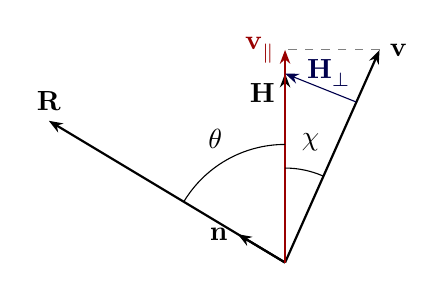
\begin{tikzpicture}[scale=0.6,>={Stealth[length=5pt]},vector/.style={->, thick},component/.style={->,thick,mydarkred}]\coordinate(O)at(0,0);\coordinate(H)at(0,4);\coordinate(V)at(2,4.5);\coordinate(Vp)at(0,4.5);\coordinate(R)at(-5,3);\coordinate(N)at(-1,0.6);\coordinate(Y)at(0,5);\draw[dashed,gray](V)--(Vp);\draw[vector](O)--(H)node[below left]{$\vb{H}$};\draw[vector](O)--(V)node[right]{$\vb{v}$};\draw[vector](O)--(R)node[above]{$\vb{R}$};\draw[vector](O)--(N)node[left] {$\vb{n}$};\draw[component](O)--(Vp)node[left]{$\vb{v}^{}_{\parallel}$};\draw[->,mydarkblue](1.5,3.4)--(H) node[midway,above,yshift=-3pt,xshift=3pt]{$\vb{H}^{}_{\perp}$};\pic[draw,"$\chi$",angle eccentricity=1.3,angle radius=1.2cm]{angle=V--O--Vp};\pic[draw,"$\theta$",angle eccentricity=1.2,angle radius=1.5cm]{angle=Vp--O--R};\end{tikzpicture}\captionof{figure}{速度和磁场的分布图}\label{f***..4}\end{center}
%我们记$\theta$为$\vb{H}$和$\vb{n}$之间的夹角,则根据立体几何自然给出$\vb{v}\cdot\vb{n}=v\cos\chi\cos\theta=v^{}_{\parallel}\cos\theta$。我们记观察点的时间间隔为$\dd{t}^{}_{\text{obs}}=\dd{t}$,则按照式(\ref{43rwgdf})我们得到观察时间间隔和辐射源的运动时间关系
%\begin{equation}\dd{t}^{}_{\text{obs}}=\qty(1-\frac{1}{c}v^{}_{\parallel}\cos\theta)\dd{t}'.\end{equation}
%在极端相对论情况下,在速度方向附近分辐射给出$\theta\approx\chi$,因此
%\begin{equation}\frac{\dd{t}^{}_{\text{obs}}}{\dd{t}'}=\qty(1-\frac{1}{c}v^{}_{\parallel}\cos\theta)^{-1}\approx\frac{1}{\sin^2\chi}>1.\end{equation}
%也就是说辐射传播的时间间隔只和纵向运动有关,且观测时间大于运动时间,这是典型的\textsl{Doppler}效应。由此我们看到“同步辐射”术语的来源:如果没有纵向运动则时间的流逝一致,即时间同步。若存在纵向运动,则必然出现\textsl{Doppler}效应,依然同步时间则会看到辐射红移。\\
%\subsubsection{远场多极矩辐射}
%\noindent 最后我们来讨论远场辐射势(\ref{retdd44})的高阶\underline{低速近似},上文中所讨论的偶极辐射是基于式(\ref{qsx5})的零阶项,我们按照相同的近似逻辑展开。依旧采用式(\ref{qsx4})的近似,我们将矢势(\ref{retdd44})写为
%$$\vb{A}(\vb{r},t)=\frac{1}{cR^{}_0}\int\vb{j}\qty(t'+\vb{r}\cdot\frac{\vb{n}}{c})\dd{V},\quad v\ll c.$$
%按类似的思路,对时间推迟项展开到一阶
%$$\vb{A}(\vb{r},t)=\frac{1}{cR^{}_0}\int\vb{j}\qty(t')\dd{V}+\frac{1}{c^2R^{}_0}\pdv{t'}\int(\vb{r}\cdot\vb{n})\vb{j}\qty(t')\dd{V},$$
%同样写为离散电荷形式,并将时间简记为$t=t'$得到
%\begin{equation}\vb{A}=\frac{1}{cR^{}_0}\dt{\vb{d}}+\frac{1}{c^2R^{}_0}\pdv{t}\sum e\vb{v}(\vb{r}\cdot\vb{n}).\label{wanerr}\end{equation}
%使用双叉积公式我们写出
%$$\vb{v}(\vb{r}\cdot\vb{n})=\vb{n}\cp(\vb{v}\cp\vb{r})-\vb{r}(\vb{v}\cdot\vb{n})=\pdv{t}\vb{r}(\vb{r}\cdot\vb{n})-\vb{r}(\vb{v}\cdot\vb{n}),$$
%类似磁矩处的操作,引入磁矩$\vb{m}$后我们得到矢势
%\begin{equation}\vb{A}=\frac{1}{cR^{}_0}\dt{\vb{d}}+\frac{1}{2c^2R^{}_0}\pdv[2]{t}\sum e\vb{r}(\vb{r}\cdot\vb{n})+\frac{1}{c^2R^{}_0}\qty(\dt{\vb{m}}\cp\vb{n}).\end{equation}
%引入\textbf{电四极矩张量}
%\begin{equation}\bm{\mathcal D}^{ab}=3\sum e\vb{r}^{a}\vb{r}^b,\end{equation}
%我们于是得到第二项写为
%$$\sum e\vb{r}^a(\vb{r}\cdot\vb{n})=\sum e\vb{r}^a\vb{r}^b\vb{n}^{}_b=\frac{1}{3}\bm{\mathcal D}^{ab}n^{}_b=\frac{1}{3}\vb{D}^a,$$
%其中矢量$\vb{D}$定义为
%\begin{equation}\vb{D}^a=\bm{\mathcal D}^{ab}n^{}_b=\mathcal D^{ij}n^{}_j\qty(\vb{e}^{}_i)^a.\end{equation}
%由于在波区内场由式(\ref{boqqu})确定,所以对矢势加任意和$\vb{n}$呈正比的项都不会改变辐射分布。\\
%\\
%所以我们将第二项写作
%$$\sum e\vb{r}(\vb{r}\cdot\vb{n})=\frac{1}{3}\sum e\qty{3\vb{r}(\vb{r}\cdot\vb{n})-\vb{n}r^2},$$
%并引入无迹的电四极矩张量
%\begin{equation}\bm{\mathcal D}^{ab}=3\sum e\vb{r}^{a}\vb{r}^b-\delta^{ab}r^2,\quad\tr(\bm{\mathcal D}^{ab})=\bm{\mathcal D}^{a}_a=0, \end{equation}
%第二项依旧写为$\vb{D}/3$。一般而言我们采用上述无迹的定义,于是矢势给出
%\begin{equation}\vb{A}=\frac{1}{cR^{}_0}\dt{\vb{d}}+\frac{1}{6c^2R^{}_0}\ddt{\vb{D}}+\frac{1}{c^2R^{}_0}\qty(\dt{\vb{m}}\cp\vb{n}).\end{equation}
%按照式(\ref{boqqu})我们计算出相应的辐射场为
%\begin{equation}\begin{aligned}&\vb{H}=\frac{1}{c^2R^{}_0}\qty{\ddt{\vb{d}}\cp\vb{n}+\frac{1}{6c}\dddt{\vb{D}}\cp\vb{n}+\qty(\ddt{\vb{m}}\cp\vb{n})\cp\vb{n}},\\&\vb{E}=\frac{1}{c^2R^{}_0}\qty{\qty(\ddt{\vb{d}}\cp\vb{n})\cp\vb{n}+\frac{1}{6c}\qty(\dddt{\vb{D}}\cp\vb{n})\cp\vb{n}+\vb{n}\cp\ddt{\vb{m}}}.\end{aligned}\label{efwvdx}\end{equation}
%辐射强度由式(\ref{qiangdd})的角分布确定,由于项的数量较多,方便期间我们从方向平均的角度考虑总强度
%$$I=\int\dd{I}^{}_{\vb{n}}=\frac{cR^2_0}{4\pi}\int\vb{H}^2\dd\textit{O}=\frac{1}{c^3}\expval{\qty{\ddt{\vb{d}}\cp\vb{n}+\frac{1}{6c}\dddt{\vb{D}}\cp\vb{n}+\qty(\ddt{\vb{m}}\cp\vb{n})\cp\vb{n}}^2}.$$
%这里简单介绍关于$\vb{H}^2$方向平均的计算方法。从单位矢量出发,对于$\vb{n}$的二次型我们写出均值
%$$\expval{n^in^j}=\frac{1}{4\pi}\int n^in^j\dd\textit{O}.$$
%因为在方向平均后,该张量是各向同性的,所以根据\textsl{Eisenhart}定理我们得到$\expval{n^in^j}\sim\delta^{ij}$。而又因为其归一性使得我们最终得到
%\begin{equation}\expval{n^in^j}=\frac{1}{4\pi}\int n^in^j\dd\textit{O}=\frac{1}{3}\delta^{ij}.\label{ggkkuu}\end{equation}
%类似的我们计算四次型,这对应$\vb{H}^2$中$\qty(\dddt{\vb{D}}\cp\vb{n})^2$的部分,根据\textsl{Eisenhart}定理给出
%$$\expval{n^in^jn^kn^l}=\frac{1}{4\pi}\int n^in^jn^kn^l\dd\textit{O}=a\delta^{ij}\delta^{kl}+b\delta^{ik}\delta^{jl}+c\delta^{il}\delta^{jk}.$$
%实际上这有点类似\textsl{Wick}定理,我们需要把度规按所有可能的乘积求和。同样按归一化,我们求得
%$$\tr(\delta^{ij}\delta^{kl})=\delta^i_i\delta^k_k+2\delta^i_k\delta^k_i=9+6=15\implies a=b=c=\frac{1}{15},$$
%因此我们得到
%\begin{equation}\expval{n^in^jn^kn^l}=\frac{1}{15}\qty(\delta^{ij}\delta^{kl}+\delta^{ik}\delta^{jl}+\delta^{il}\delta^{jk}).\end{equation}
%读者可以自行计算其余偶次方的均值,这里就不继续展示了。\\
%\\
%在此基础上我们来计算场平方项,注意到由于都是关于$\vb{n}$的叉积所以三个分项互相垂直,因而
%$$\expval{\vb{H}^2}\sim\expval{\qty(\ddt{\vb{d}}\cp\vb{n})^2}+\frac{1}{36c^2}\expval{\qty(\dddt{\vb{D}}\cp\vb{n})^2}+\expval{\qty{\qty(\ddt{\vb{m}}\cp\vb{n})\cp\vb{n}}^2}.$$
%第一项就是偶极辐射,我们可以按上述计算验证
%$$\expval{\qty(\ddt{\vb{d}}\cp\vb{n})^2}=\expval{\ddt{\vb{d}}^2}-\expval{\ddt{d}^{}_i\ddt{d}^{}_jn^in^j}=\ddt{\vb{d}}^2-\frac{1}{3}\ddt{d}^{}_i\ddt{d}^{}_j\delta^{ij}=\frac{2}{3}\ddt{\vb{d}}^2,$$
%于是最终第一项给出$I^{}_1=\dfrac{2}{3c^3}\ddt{\vb{d}}^2$,即偶极辐射的式(\ref{danctt})。类似的计算第二项
%$$\expval{\qty(\dddt{\vb{D}}\cp\vb{n})^2}=\expval{\dddt{\mathcal D}^{}_{ik}\dddt{\mathcal D}^{}_{jl}\delta^{ij}n^kn^l}-\expval{\dddt{\mathcal D}^{}_{ik}\dddt{\mathcal D}^{}_{jl}n^in^jn^kn^l}=\qty(\frac{1}{3}-\frac{2}{15})\delta^{ij}\delta^{kl}\dddt{\mathcal D}^{}_{ik}\dddt{\mathcal D}^{}_{jl}=\frac{1}{5}\dddt{\bm{\mathcal D}}^{2},$$
%其中我们简记缩并$\dddt{\bm{\mathcal D}}^{2}=\dddt{\bm{\mathcal D}}^{}_{ab}\dddt{\bm{\mathcal D}}^{ab}$。因而强度的第二项给出
%$$I^{}_2=\frac{1}{c^3}\frac{1}{36c^2}\frac{1}{5}\dddt{\bm{\mathcal D}}^{2}=\frac{1}{180c^5}\dddt{\bm{\mathcal D}}^{2}.$$
%第三项我们可以从电场给出,毕竟两者在大小上是一样的,强度自然为
%$$\expval{\qty{\qty(\ddt{\vb{m}}\cp\vb{n})\cp\vb{n}}^2}=\expval{\qty(\ddt{\vb{m}}\cp\vb{n})^2}\implies I^{}_3=\dfrac{2}{3c^3}\ddt{\vb{m}}^2.$$
%于是我们写出总强度
%\begin{equation}I=\sum_iI^{}_i=\dfrac{2}{3c^3}\ddt{\vb{d}}^2+\frac{1}{180c^5}\dddt{\bm{\mathcal D}}^{2}+\dfrac{2}{3c^3}\ddt{\vb{m}}^2.\end{equation}
%其中由于第三项和第一项的相似性,我们称$I^{}_3\sim\ddt{\vb{m}}^2$为\textbf{磁偶极辐射},而$I^{}_2$由于和四极矩有关因此称为\textbf{四级辐射}。我们注意到,两个偶极辐射的量级$I^{}_{1,3}\sim c^{-3}$,而四级辐射$I^{}_{2}\sim c^{-5}$,所以我们得到
%$$I\sim\dddt{\bm{\mathcal D}}^{2}\sim c^{-5}\ll I\sim\ddt{\vb{d}}^2\sim c^{-3},$$
%即\emph{四级辐射强度远小于偶极辐射强度,且上述关于光速的量级是普适性的}。这一点我们在引力波中还会看到,请参考第\ref{Phytvj))**}节。需要指出的是,偶极辐射的存在性要求比四级辐射更严,对磁荷质比完全相同的系统,我们有
%$$\vb{d}\sim\vb{R}^{}_m=\bm{const}t,\quad \vb{m}\sim\vb{M}=\bm{const}\implies\ddt{\vb{d}}=\ddt{\vb{m}}=\vb{0}.$$
%因而此时不存在任何偶极辐射,但四级辐射存在。\\
%\\
%我们也可以来计算辐射导致的力,由\textsl{Cauchy}应力定理我们得到观察点$R^{}_0$处的表述为
%$$F^i=\oint\sigma^{ij}\dd{S}^{}_j=\int\sigma^{ij}n^{}_jR^2_0\dd\textit{O}.$$
%应力张量可以按定义从式(\ref{70})的空间分量得到,这里直接给出结果
%\begin{equation}\vb{F}=-\frac{1}{8\pi}\int2H^2\vb{n}R^2_0\dd\textit{O}.\end{equation}
%我们同样取方向平均,当然这里是取$\expval{\vb{n}}$,和式(\ref{musilun})的操作类似。我们也直接给出最终的结果
%\begin{equation}F^{}_i=-\frac{1}{c^4}\qty{\frac{1}{15c}\dddt{\mathcal D}^{}_{ij}\ddt{d}^{\ j}+\frac{2}{3}\qty(\ddt{\vb{d}}\cp\ddt{\vb{m}})^{}_i}.\end{equation}
%读者也可以自行计算两束全同带电粒子束碰撞的总有效辐射,设入射速度为$v^{}_0$,按定义(\ref{yyu88})依旧给出结果
%\begin{equation}\varkappa=\frac{4\pi}{9}\frac{ev^3_0}{mc^5}.\end{equation}
%事实上磁偶极辐射也可以从式(\ref{hgraa})得到,读者可自行计算。关于任意参考系下的四级辐射这里就不介绍了。
%\subsection{近场偶极辐射}
%\noindent 上文中我们较为系统性的介绍了远场近似下的偶极辐射,这里我们讨论近场下的偶极辐射。所谓\textbf{近场近似},即和远场相对定义
%\begin{equation}R^{}_0\sim r\implies R^{}_0\sim R.\end{equation}
%在这种情况下,波区的概念不再适用,从而式(\ref{boqqu})也不成立,为此我们需要重新计算四维势以确定辐射场。从偶极辐射的角度出发,式(\ref{qs6})依旧成立,但标势$\varphi$并不为零。考虑到我们使用了\textsl{Lorentz}规范$\partial^{}_{\mu}A^{\mu}=0$,其给出
%$$\pdv{\varphi}{t}+\div\vb{A}=0\implies\varphi=-\int\div\vb{A}\dd{t},$$
%我们得到偶极辐射下的标势为
%\begin{equation}\varphi(t)=-\div(\frac{\vb{d}}{R^{}_0})(t').\end{equation}
%对于时间延迟$t'$,我们有时引入\textbf{\textsl{Hertz}矢量}
%\begin{equation}\vb{Z}(t)=-\frac{1}{R^{}_0}\vb{d}\qty(t-\frac{R^{}_0}{c})\implies \vb{A}=-\frac{1}{c}\dt{\vb{Z}},\quad\varphi=\div\vb{Z}.\end{equation}
%注意\textsl{Hertz}矢量满足\underline{球面波方程}
%\begin{equation}\frac{1}{c^2}\pdv[2]{t}\vb{Z}-\bm{\Delta}\vb{Z}=\square\vb{Z}=\vb{0}.\end{equation}
%需要注意这里系数$R^{-1}_0$不能从坐标偏导中提出,因为其量级$\sim R^{-1}$和原积分式相同,是体元球面波的组成部分,当然其和时间导数无关。于是按照一般的公式(\ref{emdef}),我们得到辐射场为
%\begin{equation}\begin{aligned}&\vb{H}=-\frac{1}{c}\curl\dt{\vb{Z}}=\frac{1}{c}\curl(\frac{\dt{\vb{d}}}{R^{}_0}),\\&\vb{E}=-\grad(\div\vb{Z})+\frac{1}{c}\ddt{\vb{Z}}=\grad\qty{\div(\frac{\vb{d}}{R^{}_0})}-\frac{1}{c^2}\frac{\ddt{\vb{d}}}{R^{}_0}.\end{aligned}\label{dd2Pee}\end{equation}
%使用熟知的双叉积公式
%$$\curl(\curl\vb{Z})=\grad(\div\vb{Z})-\bm{\Delta}\vb{Z},$$
%再利用球面波方程,我们得到电场为
%\begin{equation}\vb{E}=\curl(\curl\vb{Z})=\curl\qty{\curl(\frac{\vb{d}}{R^{}_0})}.\label{ddPee}\end{equation}
%用上面的结果,我们就能够求得距离和波长同量级处的场。关于辐射强度和远场内容一样,这里不再赘述。相应的我们可以计算角动量的损失速率,不难计算得到
%\begin{equation}\dv{\vb{M}}{t}=-\frac{2}{3c^3}\ddt{\vb{d}}\cp\dt{\vb{d}}.\label{Plp}\end{equation}
%其中我们使用了前文中的方向平均,这里不再展示具体过程。\\
%\\
%我们同样考虑近场的四级辐射和磁偶极辐射,并假设电偶极辐射不存在。类似式(\ref{wanerr})我们给出矢势的积分
%\begin{equation}\vb{A}=-\frac{1}{c}\int\qty(\vb{r}\cdot\grad^{}_{\vb{R}^{}_0})\frac{\vb{j}^{}_{t'}}{R^{}_0}\dd{V},\quad t'=t-\frac{R^{}_0}{c}\end{equation}
%只不过此处我们不对时间展开,因为远场近似不再适用,并且同样$R^{}_0$不能从微分中提出。交换偏导和积分,我们得到分量形式
%$$A^{}_i=-\frac{1}{c}\pdv{X^{}_j}\int \frac{x^jj^{}_i}{R^{}_0}\dd{V},$$
%其中$\vb{R}^{}_0=\vb{X}$,再次改写为离散电荷形式
%\begin{equation}A^{}_i=-\frac{1}{c}\pdv{X^{}_j}\frac{\sum ex^jv^{}_i}{R^{}_0}.\end{equation}
%按照类似的思路,我们得到以四极矩表述的形式
%\begin{equation}A^i=-\frac{1}{6c}\pdv{X^{}_j}\frac{\dt{\mathcal D}^{ij}}{R^{}_0}(t'),\quad\varphi=\frac{1}{6}\pdv{}{X^{}_i}{X^{}_j}\frac{\mathcal D^{ij}}{R^{}_0}(t').\end{equation}
%对于磁偶极辐射,我们得到
%\begin{equation}\vb{A}=\curl\qty(\frac{\vb{m}}{R^{}_0})(t'),\quad\varphi=0.\end{equation}
%不难计算出,此时磁偶极辐射场为
%\begin{equation}\vb{E}=-\frac{1}{c}\curl\qty(\frac{\vb{m}}{R^{}_0}),\quad\vb{H}=\curl\qty{\curl\qty(\frac{\vb{m}}{R^{}_0})}.\end{equation}
%对比式(\ref{ddPee})不难发现,两者在形式上是完全一致的,只不过是交换了相应的偶极矩。\\
%\\
%最后我们给出频谱形式。我们先计算磁场,在式(\ref{dd2Pee})中带入分量式,当然注意等式右侧是$t'$时刻的值,因而偶极矩的分量给出
%$$\vb{d}^{}_{\omega}e^{-i\omega t'}=\vb{d}^{}_{\omega}\exp{-i\omega\qty(t-\frac{R^{}_0}{c})}=\vb{d}^{}_{\omega}\exp{-i\omega t+ikR^{}_0)}.$$
%带入磁场中,我们得到
%\begin{equation}\vb{H}^{}_{\omega}=-ik\curl(\vb{d}^{}_{\omega}\frac{\exp(ikR^{}_0)}{R^{}_0})=ik\vb{d}^{}_{\omega}\cp\grad\frac{\exp(ikR^{}_0)}{R^{}_0}.\end{equation}
%或者,打开导数我们得到
%\begin{equation}\vb{H}^{}_{\omega}=ik\vb{d}^{}_{\omega}\cp\vb{n}\qty(\frac{ik}{R^{}_0}-\frac{1}{R^2_0})\exp(ikR^{}_0).\end{equation}
%类似的,我们得到电场为
%\begin{equation}\vb{E}^{}_{\omega}=k^2\vb{d}^{}_{\omega}\frac{\exp(ikR^{}_0)}{c}+\qty(\vb{d}^{}_{\omega}\cdot\grad)\grad\frac{\exp(ikR^{}_0)}{R^{}_0},\end{equation}
%计算导数后我们得到
%\begin{equation}\vb{E}^{}_{\omega}=\vb{d}^{}_{\omega}\qty(\frac{k^2}{R^{}_0}+\frac{ik}{R^2_0}-\frac{k}{R^{3}_0})\exp(ikR^{}_0)+\vb{n}\qty(\vb{n}\cdot\vb{d}^{}_{\omega})\qty(-\frac{k^2}{R^{}_0}-\frac{3ik}{R^2_0}+\frac{3}{R^{3}_0})\exp(ikR^{}_0).\end{equation}
%现在让我们回到波区,在远场区域我们可以忽略上述$R^{-n}_0,\ n\geq2$的高阶项,从而给出
%\begin{equation}\begin{aligned}&\vb{E}^{}_{\omega}=\frac{k^2}{R^{}_0}\qty{\vb{d}^{}_{\omega}-\vb{n}\qty(\vb{n}\cdot\vb{d}^{}_{\omega})}\exp(ikR^{}_0)=\frac{k^2}{R^{}_0}\vb{n}\cp\qty(\vb{d}^{}_{\omega}\cp{n})\exp(ikR^{}_0),\\&\vb{H}^{}_{\omega}=-\frac{k^2}{R^{}_0}\vb{d}^{}_{\omega}\cp\vb{n}\exp(ikR^{}_0).\end{aligned}\end{equation}
%而在超近场近似$kR^{}_0\ll1$下,我们忽略$R^{-n}_0,\ n\leq2$的低阶项,并令$\exp(ikR^{}_0)\approx1$,于是得到电场为
%\begin{equation}\vb{E}^{}_{\omega}=\frac{1}{R^3_0}\qty{3\vb{n}\qty(\vb{n}\cdot\vb{d}^{}_{\omega})-\vb{d}^{}_{\omega}}.\end{equation}
%可以看到,这类似式(\ref{surssa})的诱导磁场,事实上这就是电偶极矩的诱导电场公式。
%\subsection{电磁辐射阻尼简介}\label{Fyyv.'}
%\noindent 前面我们介绍了低速电荷云系统的二阶修正\textit{Lagrangian}(\ref{hi2gdd}),现在我们考虑更高阶的修正。首先需要指出的是,在上文中我们看到,偶极辐射的能量(\ref{danctt})量级为$\sim c^{-3}$,而由于\textit{Lagrangian}对四维势能本身带$\sim c^{-1}$,因此二阶修正已经可以描述绝大部分的辐射体系。由此我们推测,高阶修正应该能给出体系的内蕴现象,并且这些现象和对外辐射相关。\\
%\subsubsection{辐射系统的三级修正和Abraham-Lorentz力}
%\noindent 类似式(\ref{efeg44}),我们对推迟标势展开到三阶$\sim c^{-3}$,当然同样的,对于矢势我们只需要展开到二阶即可。具体的过程这里就不展示了,直接给出相应的结果
%$$\begin{aligned}&\varphi^{(3)}=-\frac{1}{6c^3}\pdv[3]{t}\int R^2\rho \dd{V},\\&\vb{A}^{(2)}=-\frac{1}{c^2}\pdv{t}\int\vb{j}\dd{V}.\end{aligned}$$
%我们依旧按照同样的理由,选取规范使得标势只含静电场部分,即令$\varphi^{(3)}=0$。类似的我们写出规范函数$f$如下
%$$\frac{1}{c}\pdv{f}{t}=-\frac{1}{6c^3}\pdv[3]{t}\int R^2\rho \dd{V}\implies f=-\frac{1}{6c^2}\pdv[2]{t}\int R^2\rho \dd{V}.$$
%于是矢势给出
%$$\vb{A}^{(2)}=-\frac{1}{c^2}\pdv{t}\int\vb{j}\dd{V}-\frac{1}{6c^2}\pdv[2]{t}\grad\int R^2\rho\dd{V}=-\frac{1}{c^2}\pdv{t}\int\vb{j}\dd{V}-\frac{1}{3c^2}\pdv[2]{t}\int \vb{R}\rho\dd{V},$$
%注意这里梯度不对常值电荷密度$\rho$起作用。方便起见,我们依旧使用离散电荷体系计算,写出$\vb{R}=\vb{R}^{}_0-\vb{r}$,两个积分给出
%$$\pdv{t}\int\vb{j}\dd{V}=\sum_ae^{}_a\dt{\vb{v}}^{}_a=\ddt{\vb{d}},\quad\pdv[2]{t}\int\vb{R}\rho\dd{V}=-\pdv[2]{t}\int\vb{r}\rho\dd{V}=-\sum_ae^{}_a\dt{\vb{v}}^{}_a.$$
%因而我们最终得到矢势的二阶修正为
%\begin{equation}\vb{A}^{(2)}=-\qty(\frac{1}{c^2}-\frac{1}{3c^2})\sum_ae^{}_a\dt{\vb{v}}^{}_a=-\frac{2}{3c^2}\ddt{\vb{d}},\quad\varphi^{(2)}=0.\end{equation}
%相应的,我们计算电场的修正(注意这是三阶修正)得到
%$$\vb{E}^{(3)}=-\frac{1}{c}\pdv{t}\vb{A}^{(2)}=\frac{2}{3c^3}\dddt{\vb{d}}\sim\dt{\vb{w}},$$
%可见三阶修正项和加速度的速度有关。这种结构在通常的场中并不显然,因为根据第二定律,力只和加速度相关。\\
%\\
%因此这样的结构会导致一种新类型的力,暂时仍记为$\vb{f}$,对于电荷云内的单个电荷其写为
%\begin{equation}\vb{f}=e\vb{E}^{(3)}=\frac{2e}{3c^3}\dddt{\vb{d}}.\label{dangedd}\end{equation}
%为了理解这个力的物理含义,我们考虑其时均功率(即前文中的强度),根据经典力学我们写出电荷云下
%$$\expval{P}^{}_t=\sum_a\expval{\vb{f}^{}_a\cdot\vb{v}^{}_a}^{}_t=\frac{2}{3c^3}\expval{\dddt{\vb{d}}\cdot\sum_ae^{}_a\vb{v}^{}_a}^{}_t=\frac{2}{3c^3}\expval{\dddt{\vb{d}}\cdot\dt{\vb{d}}}^{}_t,$$
%对时间的全导在时均下为零,我们选择对三阶导展开微分,最终我们求得总功率为
%\begin{equation}\expval{P}^{}_t=-\frac{2}{3c^3}\expval{\ddt{\vb{d}}^2}^{}_t.\end{equation}
%回顾到偶极辐射的耗散能流(\ref{danctt}),我们得到
%\begin{equation}\expval{P}^{}_t+\expval{I}^{}_t=0\implies P=\sum_a\vb{f}^{}_a\cdot\vb{v}^{}_a=-I.\end{equation}
%这说明上述这种力对于电荷体系的作用是电磁辐射的反作用,根据一般运动体系中反作用力的效果,我们称此类现象为\textbf{辐射阻尼 \textit{Radiation Damping}},并称相应的阻尼力为\textbf{\textsl{Abraham-Lorentz}力}。相对应这种力,我们来计算系统角动量$\vb{M}$的变化,根据经典力学下的角动量定理,我们得到
%$$\dv{\vb{M}}{t}=\sum_a\vb{f}^{}_a\cp\vb{r}^{}_a=\frac{2}{3c^3}\dddt{\vb{d}}\cp\vb{d},$$
%同样的计算时均值,仍然对三阶导展开微分,省略全导数后我们得到
%\begin{equation}\expval{\dv{\vb{M}}{t}}^{}_t=-\frac{2}{3c^3}\expval{\ddt{\vb{d}}\cp\dt{\vb{d}}}^{}_t.\end{equation}
%注意到其和式(\ref{Plp})的结果是相同的,这进一步说明了该力起到阻尼现象。考虑到这个力的符号是正的,说明所谓的“阻尼力”实际上是推力,对于电荷而言就是动量守恒的结果,阻尼是相对于电磁辐射的运动而言的。\\
%\\
%现在我们来深入的探讨\textsl{AL}力的力学特性。对于单电荷系统,我们从式(\ref{dangedd})得到力为
%\begin{equation}\vb{f}=\frac{2e^2}{3c^3}\ddt{\vb{v}}.\label{ef2344}\end{equation}
%在静止参考系中,我们令观察点趋向电荷,也即$\vb{R}\rightarrow\vb{0}$,则容易从式(\ref{efeg44})看出,所有的高阶项$\sim R$均消失。因此我们可以说,式(\ref{ef2344})就是电荷在其静系下的辐射反作用力的准确公式。于是在静系下,无外场时电荷的运动方程即为
%\begin{equation}m\dt{\vb{v}}=\vb{f}=\frac{2e^2}{3c^3}\ddt{\vb{v}}.\label{;sd;;}\end{equation}
%可以看到,方程的非平凡解为加速度$\dt{\vb{v}}\sim\exp(\dfrac{3mc^3}{2e^2}t)$,即加速度随时间无限增加。这一点明显违反无外场时的能量守恒,其产生必然源于对运动方程的理解。在数学上令$m=0$,则我们得到$\dt{\vb{v}}=\vb{const}$,又因为无外场我们必然有$\dt{\vb{v}}=\vb{0}$。这就说明上述悖论的产生是质量的理解问题,下面简单讨论一下。\\
%\\
%我们已经看到,运动方程(\ref{;sd;;})成立的充要条件为$m=0$,但在物理上电荷的质量必然非零,因而在某种程度上我们可以认为,电荷的质量可分为两部分。基于电荷作用量$S=S^{}_p+S^{}_{pf}$,我们称这两个质量为
%\begin{itemize}\item\textbf{固有质量 \textit{Proper Mass}}:$m^{}_p$,电荷作为自由粒子的内禀质量,不参与相互作用,由\textit{Lagrangian}定义为$L=-m^{}_pc^2\dfrac{\dd s}{\dd t}$;\item\textbf{电磁质量 \textit{EM Mass}}:$m^{}_{em}$,电荷和电磁场的相互作用的体现,是一种等效质量,由总四维辐射动量(\ref{meiyon2e]})确定。需要强调的是,总动量给出电荷的总质量$m$,因此我们有$m^{}_{em}=m-m^{}_p$。\end{itemize}
%回到运动方程(\ref{;sd;;}),不难发现悖论产生的原因:由于式中$m$为总质量,但真正参与耦合运动的只是电磁质量,因而我们相当于多出了固有质量的运动。而固有质量在相对论力学下是无穷大的,也就是这一部分导致了悖论。我们不妨在外场下进一步讨论该力,算上经典洛伦兹力(\ref{emfff})我们得到运动方程
%\begin{equation}m\dt{\vb{v}}=e\vb{E}+\frac{e}{c}\vb{v}\cp\vb{H}+\frac{2e^2}{3c^3}\ddt{\vb{v}},\end{equation}
%基于上述的讨论我们知道,阻尼力应作为电磁力的扰动出现,这样才能保证系统的有限性。\\
%\
%为了理解该扰动的定义,我们做类似第\ref{landtoo908}节的讨论。在没有阻尼力扰动的情况下,考虑静系下速度的二阶导为
%$$\ddt{\vb{v}}=\frac{e}{m}\dt{\vb{E}}+\frac{e}{mc}\dt{\vb{v}}\cp\vb{H},$$
%这里我们假设矢势$\vb{A}$和时间无关。对加速度带入同样精度$\dt{\vb{v}}=\dfrac{e\vb{E}}{m}$,我们得到\textsl{AL}力以纯外场写为
%\begin{equation}\vb{f}=\frac{2e^3}{3mc^3}\dt{\vb{E}}+\frac{2e^4}{3m^2c^4}\vb{E}\cp\vb{H}.\label{AFggb}\end{equation}
%假设电荷处于封闭运动,记运动频率为$\omega$,则$\dt{\vb{E}}\sim\omega\vb{E}$。于是第一项远小于电场力$e\vb{E}$写为
%\begin{equation}\frac{2e^3\omega}{3mc^3}\ll e\implies\lambda\gg\frac{e^2}{mc^2}=r{}_e,\quad\lambda\sim\frac{c}{\omega}.\end{equation}
%可见阻尼力只适用于辐射波长远大于经典半径$r{}_e$的电荷上。可以看到,与$r{}_e$同量级的距离会导致电磁场的内在矛盾。类似的,我们将第二项也和电场力$e\vb{E}$对比,给出
%\begin{equation}\frac{2e^4}{3m^2c^4}H\ll e\implies H\ll\frac{m^2c^4}{e^3}\text{或}\frac{c}{\omega^{}_H}\gg r^{}_e\label{zhajiii}\end{equation}
%因此扰动只适用于弱场情况,这和\textsl{Landau}理论的结论是类似的。\\
%\subsubsection{四维辐射阻尼力}
%\noindent 在详细分析了三维\textsl{AL}力后,我们来考察其四维协变形式。后续的推导内容和第\ref{Fyyv.'3}节是十分类似的,这里我们介绍一下计算思路。\\
%\\
%力的四维形式由式(\ref{si3zhiqq})确定,在国际单位制下其具体时空分量为
%\begin{equation}g^{\mu}=\qty(\frac{\vb{f}\cdot\vb{v}}{c^2\sqrt{1-\dfrac{v^2}{c^2}}},\frac{\vb{f}}{c\sqrt{1-\dfrac{v^2}{c^2}}}),\quad g^{\mu}u^{}_{\mu}=0.\end{equation}
%根据一般的理论,静系对应低速近似,当然这里依旧只能考虑单点电荷情况,因此从式(\ref{dangedd})得到
%$$\lim_{v\to 0}g^{\mu}=\qty(0,\frac{\vb{f}}{c})=\qty(0,\frac{2e^2}{3c^4}\dv[2]{\vb{v}}{t}).$$
%为了将上式变为四维单位形式,我们利用静系下的三维加速度$c^2\vb{w}=\dt{\vb{v}}$,于是一个显然的解为
%\begin{equation}g^{\mu}_l=\frac{2e^2}{3c}\dv[2]{u^{\mu}}{s}.\end{equation}
%但我们需要注意,四维力满足正交性条件$g^{\mu}u^{}_{\mu}=0$,上述形式显然不符。为此我们添加一个辅助矢量$C^{\mu}$,满足
%$$\lim\limits_{v\to 0}C^{i}=0,\quad \qty(g^{\mu}_l+C^{\mu})u^{}_{\mu}=0\implies C^{\mu}u^{}_{\mu}=-\frac{2e^2}{3c}u^{}_{\mu}\dv[2]{u^{\mu}}{s}.$$
%第一条保证了辅助矢量不影响到低速近似的结论,回顾到低速下四维速度$u^{\mu}=(1,0,0,0)$,不难想到其应该有形式$C^{\mu}\sim u^{\mu}$。第二条确定了正交性关系,又因为$u^{\mu}u^{}_{\mu}=1$最终我们得到
%\begin{equation}C^{\mu}=-\frac{2e^2}{3c}u^{\mu}u^{}_{\nu}\dv[2]{u^{\nu}}{s},\end{equation}
%从而四维阻尼力为
%\begin{equation}g^{\mu}=g^{\mu}_l+C^{\mu}=\frac{2e^2}{3c}\qty(\dv[2]{u^{\mu}}{s}-u^{\mu}u^{}_{\nu}\dv[2]{u^{\nu}}{s}).\label{dairrru}\end{equation}
%我们可以从四维动量角度证明上述的正确性,这里考虑无穷远处$\partial\mathscr M$的情况。由于边界处场渐进消失,因此加速度$\eval{w^{\mu}}_{\partial\mathscr M}=0$,由动量定理我们得到四维阻尼力确定的四维动量变化为
%$$\begin{aligned}\Delta P^{\mu}_g&=\int g^{\mu}\dd s=\frac{2e^2}{3c}\int\qty(\dv[2]{u^{\mu}}{s}-u^{\mu}u^{}_{\nu}\dv[2]{u^{\nu}}{s})\dd s\\&=\frac{2e^2}{3c}\eval{\qty(\dv{u^{\mu}}{s}-u^{\mu}u^{}_{\nu}\dv{u^{\nu}}{s})}_{\partial\mathscr M}+\frac{2e^2}{3c}\int\dv{u^{}_{\nu}}{s}\dv{u^{\nu}}{s}u^{\mu}\dd s\\&=\frac{2e^2}{3c}\int\dv{u^{}_{\nu}}{s}\dv{u^{\nu}}{s}\dd{x}^{\mu}.\end{aligned}$$
%对比辐射动量(\ref{xse660}),我们看到$\Delta P^{\mu}_g+\Delta P^{\mu}=0$,再次证明了上述为阻尼效应。\\
%\\
%和前文中的理解类似,该力同样只能以扰动出现在若外场中,我们也能用类似式(\ref{AFggb})的思路,以外场表示上述的力。引入电荷的四维运动方程(\ref{shi337}),我们给出速度的一阶导和二阶导
%$$\dv{u^{\mu}}{s}=\frac{e}{mc^2}F^{\mu\nu}u^{}_{\nu}\implies\dv[2]{u^{\mu}}{s}=\frac{e}{mc^2}\qty(\dv{F^{\mu\nu}}{s}u^{}_{\nu}+F^{\mu\nu}\dv{u^{}_{\nu}}{s})=\frac{e}{mc^2}\partial^{}_{\gamma}F^{\mu\nu}u^{}_{\nu}u^{}_{\gamma}+\frac{e^2}{m^2c^4}F^{\mu\nu}F^{}_{\nu\delta}u^{\delta}.$$
%带入式(\ref{dairrru}),并注意$F^{\mu\nu}$的反对称性,我们得到外场下的\textbf{\textsl{Landau-Lifchitz}阻尼力}
%\begin{equation}\vb{g}^{A}=\frac{2e^3}{3mc^3}\partial_C\vb{F}^{AB}u^{}_Bu^C-\frac{2e^4}{3m^2c^5}\vb{F}^{AB}\vb{F}^{}_{CB}u^C+\frac{2e^4}{3m^2c^5}\qty(\vb{F}^{BC}u^{}_C)\qty(\vb{F}^{}_{BD}u^D)u^A.\end{equation}
%经过一些冗长的计算,我们给出\textsl{LL}阻尼力的三维分量,具体推导过程请读者自行给出
%\begin{equation}\begin{aligned}\vb{f}=&\frac{2e^3}{3mc^3}\qty(1-\dfrac{v^2}{c^2})^{-1/2}\qty{\qty(\pdv{t}+\vb{v}\cdot\grad)\vb{E}+\frac{\vb{v}}{c}\cp\qty(\pdv{t}+\vb{v}\cdot\grad)\vb{H}}\\&+\frac{2e^2}{3m^2c^4}\qty{\vb{E}\cp\vb{H}+\frac{1}{c}\vb{H}\cp(\vb{H}\cp\vb{v})+\frac{1}{c}\vb{E}(\vb{v}\cdot\vb{E})}\\&-\frac{2e^2\vb{v}}{3m^2c^5}\qty(1-\dfrac{v^2}{c^2})^{-1}\qty{\qty(\vb{E}+\frac{\vb{v}}{c}\cp\vb{H})^2-\frac{1}{c^2}\qty(\vb{E}\cdot\vb{v})^2}.\end{aligned}\end{equation}
%现在我们分析极端相对论情况,此时$u^{\mu}=\infty$,因此\textsl{LL}阻尼力以包含速度三重幂的第三部分为主。提出该部分,并带入光速$v=c$,我们得到此时的三维阻尼力为
%\begin{equation}\vb{f}=\frac{2e^4}{3m^2c^4}\qty(\vb{F}^{BC}u^{}_C)\qty(\vb{F}^{}_{BD}u^D)\vb{n},\end{equation}
%其中$\vb{n}$是速度方向的单位向量。设粒子沿$x$轴运动,并在除了\textsl{Lorentz}系数外都带入$v=c$,我们得到具体量为
%\begin{equation}f^{}_x=-\frac{2e^4}{3m^2c^4}\frac{\qty(E^{}_y-H^{}_z)^2+\qty(E^{}_z+H^{}_y)^2}{1-\dfrac{v^2}{c^2}}\sim\qty(1-\dfrac{v^2}{c^2})^{-1}=\mathscr E^2.\label{dair23u}\end{equation}
%我们看到,此时阻尼力和能量平方成正比。若考虑低速近似,则其和速度的四次方成正比,但是要注意这仍然比空气阻力小。如果我们用马赫数$Ma$表示,则这里的低速近似为$Ma\ll1$,因此$\sim u^4\ll u^2$。\\
%\\
%前面曾指出,在静系下外场须满足式(\ref{zhajiii})才存在阻尼效应,现在我们将其推广至任意参考系。记场在速度为$v$的惯性参考系中的量级为$F$,则变换到静系下,带入式(\ref{zhajiii})我们得到
%\begin{equation}\frac{F}{\sqrt{1-\dfrac{v^2}{c^2}}}\ll\frac{m^2c^4}{e^3},\label{;da;ir23u}\end{equation}
%这就是相对论性场约束。同时若我们关注极端相对论阻尼力,将式(\ref{dair23u})的量级和外力$\sim eF$相比我们得到
%$$\lim_{v\to c}\frac{\vb{f}}{eF}\sim\lim_{v\rightarrow c}\frac{e^3F}{m^2c^4\qty(1-\dfrac{v^2}{c^2})}=\infty,$$
%可见在极端相对论下,粒子的主要外力是阻尼力,于是沿运动$x$向的能量损失方程写为
%\begin{equation}-\dv{\mathscr E}{x}=f^{}_x=k(x)\mathscr E^2.\end{equation}
%其中我们将比例系数记为$k(x)$,其为坐标的函数,按照式(\ref{dair23u})的各具体量表示。若粒子的初始位置为$x^{}_0$,能量为$\mathscr E^{}_0$,终点为$\mathscr E^{}_1(x^{}_1)$,则上述方程的解为
%\begin{equation}\frac{1}{\mathscr E^{}_1}=\frac{1}{\mathscr E^{}_0}+\int^{x^{}_1}_{x^{}_0}k(x)\dd{x}.\end{equation}
%若粒子的运动跨越了整个场(无边界,$x^{}_0=-\infty,x^{}_1=\infty$),则上述等式写为
%\begin{equation}\frac{1}{\mathscr E^{}_1}=\frac{1}{\mathscr E^{}_0}+\int_{\mathbb R}k(x)\dd{x}.\end{equation}
%由于此时$\mathscr E^{}_0=\infty$,因此我们看到终态能量趋向一个常数
%$$\frac{1}{\mathscr E^{}_{cr}}=\int_{\mathbb R}k(x)\dd{x},$$
%具体带入我们得到
%\begin{equation}\frac{1}{\mathscr E^{}_{cr}}=\frac{2}{3m^2c^4}\qty(\frac{e^2}{mc^2})^2\int_{\mathbb R}\qty{\qty(E^{}_y-H^{}_z)^2+\qty(E^{}_z+H^{}_y)^2}\dd{x}.\end{equation}
%读者可自行计算与此相应的,双电荷接触所需的时间,这里不再过多介绍。\\
%\\
%关于极端相对论粒子的进一步分析这里就不给出了,具体可以参考\cite{L41}的\S76。这里我们只强调一下,条件(\ref{;da;ir23u})是外场下极端相对论存在的充要条件,并且此时阻尼力做的功和粒子总能量处于一个量级。
%\subsection{电磁波的散射}
%\noindent 前面我们系统性的介绍了电磁波的产生机制,以及各类衍生效应。但我们也知道,电磁波作为外场会诱导电荷运动,对于单电荷其在单色波中的运动方程由式(\ref{d2Dfb})控制。从其形式不难看出这是变速运动,因而根据前文所述,必然会产生电磁辐射。而且辐射波总体来讲是部分偏振的,因此作为外场的电磁波和由此辐射出的电磁波之间并不相同。\\
%\\
%上述的这种现象称为\textbf{电磁波的散射 \textit{Scattering of EM wave}},是散射现象的一种微观解释,它将现象归结为电荷对电磁波的响应。一般而言,我们将作为外场的电磁波称为\textbf{入射波},辐射导致的电磁波称为\textbf{散射波},以此和光学中的散射现象相对应。需要注意的是,由于辐射是球面波,所以这不可能是反射。并且电磁辐射是单次瞬时发射,所以也不是衍射现象,对于这些区别应该有正确的认识。
%\subsubsection{单个电荷的散射}
%\noindent 我们从单个静止的电荷开始,先建立关于散射的基本理论框架,再推广到运动电荷。\\
%\\
%对于散射,最简单的描述方法便是有效截面。类似韧致辐射中定义有效辐射(\ref{yyu88})的瞄准距离,我们将有效截面定义为散射波能量密度和入射波的能量比。根据前文所定义的各类物理量来看,最直接的方法便是用能流,用经典碰撞理论的记号写为
%\begin{equation}\dd\sigma^{}_{\vb{n}}=\expval{\frac{\dd I^{}_{\vb{n}}}{\abs{\vb{\mathcal S}}}}_t,\label{ddi..98}\end{equation}
%其中$\vb{\mathcal S}$是入射波的能流密度,$\dd I^{}_{\vb{n}}$是向$\vb{n}$向散射波的强度,这里取时均值是为了囊括部分偏振波。我们暂时只考虑入射波为单色平面波,其电场为
%$$\vb{E}=\vb{E}^{}_0\cos(\vb{k}\cdot\vb{r}-\omega t+\alpha).$$
%我们\underline{假设该入射波很弱},使得电荷以低速运动,则电磁力基本就是$e\vb{E}$。在这种情形下,我们可以忽略电荷对电磁波的影响,从而可以认为电场和空间无关。于是电场可以取为原点处的值
%\begin{equation}\vb{E}=\vb{E}^{}_0\cos(\omega t-\alpha).\end{equation}
%此时电荷的运动方程为$m\ddt{\vb{r}}=e\vb{E}$,于是偶极矩的二阶导给出
%\begin{equation}\ddt{\vb{d}}=e\ddt{\vb{r}}=\frac{e^2}{m}\vb{E}.\end{equation}
%由于现在是低速近似,因此我们可以使用远场偶极辐射描述散射波,从而强度由式(\ref{d33tt})确定为
%\begin{equation}\dd I^{}_{\vb{n}}=\frac{e^4}{4\pi m^2c^3}\qty(\vb{E}\cp\vb{n}')^2\dd\textit{O}=\frac{e^4}{4\pi m^2c^3}\sin^2\theta\abs{\vb{E}}^2\dd\textit{O}.\label{feoon}\end{equation}
%其中$\vb{n}'$是散射波的单位方向,$\theta=\expval{\widehat{\vb{E},\vb{n}'}}$。不难注意到,由于辐射通过运动方程和入射波直接相关,因而两者的频率必然相同。入射波的能流密度只考虑电场即可,于是我们得到
%$$\abs{\vb{\mathcal S}}=\frac{c}{4\pi}\abs{\vb{E}}^2.$$
%最终单位有效截面给出
%\begin{equation}\dd\sigma^{}_{\vb{n}}=\frac{e^4}{4\pi m^2c^3}\frac{4\pi}{c}\frac{\sin^2\theta\abs{\vb{E}}^2\dd\textit{O}}{\abs{\vb{E}}^2}=\qty(\frac{e^2}{mc^2})^2\sin^2\theta\dd\textit{O}.\label{quns2s}\end{equation}
%总有效截面$\sigma$自然是单位有效截面的积分,将角元写为$\dd\textit{O}=\sin\theta\dd\theta\dd\phi$,积分后得到
%\begin{equation}\sigma=\int\dd\sigma^{}_{\vb{n}}=\frac{8\pi}{3}\qty(\frac{e^2}{mc^2})^2=\frac{8\pi}{3}r^2_e.\label{qunss}\end{equation}
%这个结论称为\textbf{\textit{Thomson}公式},其可以通过\textsl{Compton}散射公式取低速近似得到,这里不做说明。\\
%\\
%这里我们简单的列举几个例子,并介绍运动电荷的散射模型。
%\begin{enumerate}\item 对于椭圆波,我们将其电场在原点处写为$\vb{E}=\vb{A}\cos(\omega t-\alpha)+\vb{B}\sin(\omega t-\alpha)$,其中$\vb{A}$和$\vb{B}$是相互垂直的常矢量,分别确定两个线偏振。替换式(\ref{feoon})中的电场矢量,我们立马得到有效截面\begin{equation}\dd\sigma^{}_{\vb{n}}=\qty(\frac{e^2}{mc^2})^2\frac{\qty(\vb{A}\cp\vb{n}')^2+\qty(\vb{B}\cp\vb{n}')^2}{A^2B^2}\dd\textit{O}.\end{equation}如果我们记$\theta=\expval{\widehat{\vb{A},\vb{n}'}}$,则$\vb{B}$和$\vb{n}'$的夹角$\theta'$确定为$\cos\theta'=\sin\theta\sin\alpha$,其中$\alpha=\expval{\widehat{\vb{n},\vb{n}'}}$是入射波和散射波之间的夹角。此时角元为$$\dd\textit{O}=\sin\alpha\dd\alpha\dd\theta,\quad0\leq\alpha\leq\pi,\quad0\leq\theta\leq2\pi,$$总有效截面就在上述取值限下取积分给出,请读者自行计算。\item 现在考虑运动电荷的散射。由于此时散射源在运动,所以必然存在\textbf{\textsl{Doppler}效应},简而言之就是观察者和源本身的频率不同,可以通过四维波矢的\textsl{Lorentz}变化得到。此处我们所考察的是入射波和散射波的频率差,因而类似的写出不变量\begin{equation}k^{\text{入}}_{\mu}u^{\mu}=const=k^{\text{散}}_{\mu}u^{\mu},\end{equation}其中左侧是入射波量,右侧是散射波量,当然电荷的四维速度是相同的。设电荷三维速度为$\vb{v}$,相应的频率为$\omega^{}_{\text{入}},\omega^{}_{\text{散}}$,相应波矢和速度的夹角为$\theta^{}_{\text{入}},\theta^{}_{\text{散}}$,则不变量的具体展开式为\begin{equation}\omega^{}_{\text{入}}\qty(1-\frac{v}{c}\cos(\theta^{}_{\text{入}}))=\omega^{}_{\text{散}}\qty(1-\frac{v}{c}\cos(\theta^{}_{\text{散}})).\label{1wqd23oo}\end{equation}可见若入射波垂直于粒子运动方向打入,则散射波的频率变化完全依赖于散射方向,这是加速度和速度平行的结果,也就是散射波的\textsl{Doppler}效应。关于散射导致的频率变换,我们后续在电荷云中做详细探讨。\item 承接上述运动粒子模型,我们来考察入射线偏振波。假设入射方向和粒子的运动方向吻合,则电磁场也即加速度与速度垂直,散射强度由式(\ref{naaa2})控制,当然三维加速度需要用入射波外场给出\begin{equation}\vb{w}=\dt{\vb{v}}=\frac{e}{m}\sqrt{1-\frac{v^2}{c^2}}\qty{\vb{E}+\frac{\vb{v}}{c}\cp\vb{H}-\frac{\vb{v}}{c^2}\vb{v}\cdot\vb{E}}.\end{equation}这个公式的推导留给读者自行证明。入射波的能流密度不难得到,就是\textsl{Poynting}矢量的模,于是有效截面给出\begin{equation}\dd\sigma^{}_{\vb{n}}=\qty(\frac{e^2}{mc^2})^2\frac{\qty(1-\dfrac{v^2}{c^2})\qty(1-\dfrac{v}{c})^2}{\qty(1-\dfrac{v}{c}\cos\theta)^6}\qty{\qty(1-\dfrac{v}{c}\sin\theta\cos\phi)^2-\qty(1-\dfrac{v^2}{c^2})\cos^2\theta}(t')\dd\textit{O}.\end{equation}此处相应的角度参数含义均不变,当然仍需注意等式右侧是取$(t')$瞬时散射时刻的值。\item 现在我们来考察微振动电荷对线偏振波的散射,暂时不考虑辐射的反作用力。记电荷的固有频率为$\omega^{}_0$,入射波频率为$\omega$,则在弱场的前提下,电荷谐振子只受电场力,其运动方程写出\begin{equation}\dv[2]{\vb{r}}{t}+\omega^2_0\vb{r}=\frac{e}{m}\vb{E}^{}_0\cos(\omega t).\label{li11}\end{equation}这是典型的单参强迫振动方程,其解为\begin{equation}\vb{r}=\frac{e}{m}\frac{\vb{E}^{}_0\cos(\omega t)}{\omega^2_0-\omega^2}.\end{equation}计算出相应的散射场$\ddt{\vb{d}}=e\ddt{\vb{r}}$,我们得到有效截面为\begin{equation}\dd\sigma^{}_{\vb{n}}=\qty(\frac{e^2}{mc^2})^2\frac{\omega^4}{(\omega^2_0-\omega^2)^2}\sin^2\theta\dd\textit{O}=\qty(\frac{e^2}{mc^2})^2\qty(\dfrac{\omega^2_0}{\omega^2}-1)^{-2}\sin^2\theta\dd\textit{O},\quad \theta=\expval{\widehat{\vb{E},\vb{n}'}}.\label{li1231}\end{equation}我们还可以类似的得到电偶极转子的散射,假设转子的频率$\Omega^{}_0\ll\omega$,同时令其是各项同性的,则在对$\ddt{\vb{d}}^2$方向平均后我们直接给出总截面\begin{equation}\sigma=\frac{16\pi d^4}{9c^4J^2}.\end{equation}其中$J$转子的转动惯量,其具体的力学细节请参考\cite{L6f}。\end{enumerate}
%这里我们没有分析运动电荷对椭圆波的散射,请读者自行给出,只需要做类似第一种模型的分解即可。\\
%\\
%现在来讨论散射导致的反作用力。由于我们现在考察对象是电荷,所以最简单的方法便是计算单位时间的动量损失。根据正则能动密度张量定义(\ref{8h7g7u})及其相应的守恒律,入射波在电荷上的动量损失为
%$$\dd\vb{P}=\sigma\expval{\epsilon}^{}_t\vb{n}\dd t,$$
%其中$\expval{\epsilon}^{}_t$是入射波时均能量密度,$\sigma$是总有效截面,$\vb{n}$是入射波单位方向。这个等式可以通过一般的散射理论得到,此处不做过多说明。其次,前文中已说明在低速近似下,偶极辐射无动量损失(\ref{23LDM}),因而由动量定理,电荷所受的平均反力为
%\begin{equation}\expval{\vb{f}}^{}_t=\sigma\expval{\epsilon}^{}_t\vb{n}.\end{equation}
%假设入射波沿$x$轴传播,则在静止参考系$K^{}_0$下粒子所受加速度为$mw^{}_0=\sigma\expval{\epsilon}^{}_t$。若粒子在系$K$中有速度$v$,且则通过$K^{}_0\rightarrow K$的\textsl{Lorentz}变换我们得到运动方程
%$$\dv{t}\frac{v}{\sqrt{1-\dfrac{v^2}{c^2}}}=\qty(1-\dfrac{v^2}{c^2})^{-3/2}\dv{v}{t}=\frac{\sigma\expval{\epsilon}^{}_t}{m}\frac{\qty(1-\dfrac{v}{c})^2}{1-\dfrac{v^2}{c^2}}=\frac{\sigma\expval{\epsilon}^{}_t}{m}\frac{1-\dfrac{v}{c}}{1+\dfrac{v}{c}}.$$
%令初始条件为$v(t=0)=0$,我们得到解为
%\begin{equation}\frac{\sigma\expval{\epsilon}^{}_t}{mc}t=\frac{1}{3}\qty(\frac{2-\dfrac{v}{c}}{1-\dfrac{v}{c}}\sqrt{\frac{1+\dfrac{v}{c}}{1-\dfrac{v}{c}}}-2).\end{equation}
%再根据速度定义$v=\dv*{x}{t}$变能解出运动轨迹,请读者自行计算。\\
%\\
%上述力的反作用性,不难联想到在低速近似下,辐射阻尼导致的\textsl{AL}力。我们同样来计算其时均值,对外场式(\ref{AFggb})取时均值,第一项对时间的全导消失,第二项在波区中给出$\vb{E}\cp\vb{H}=E^2\vb{n}$,因而得到
%\begin{equation}\expval{\vb{f}^{}_{AL}}^{}_t=\frac{2e^4}{3m^2c^4}\expval{E^2\vb{n}}^{}_t=\frac{8\pi}{3}\qty(\frac{e^2}{mc^2})^2\frac{\expval{E^2}^{}_t}{4\pi}\vb{n}.\end{equation}
%由于式(\ref{qunss})我们看到,前两项即为\textsl{Thomson}公式确定的截面,第三项是电磁波的时均能量密度$\expval{\epsilon}^{}_t$,于是上式写为
%$$\expval{\vb{f}^{}_{AL}}^{}_t=\sigma\expval{\epsilon}^{}_t\vb{n}=\expval{\vb{f}}^{}_t,$$
%可见散射的反作用的确体现为阻尼效应。由此便能确定弱入射波场的具体量级,根据第\ref{Fyyv.'}节的介绍我们知道其应满足$\expval{\vb{f}}^{}_t\ll e\vb{E}$。而$e\vb{E}$是入射波对电荷的直接作用力,因此反作用力相较于入射波场是二级量,符合常理。由此我们进一步计算考虑反作用力的散射模型,比如例四的运动方程(\ref{li11})现在写为
%\begin{equation}\dv[2]{\vb{r}}{t}+\omega^2_0\vb{r}=\frac{e}{m}\vb{E}^{}_0\exp(-i\omega t)+\frac{2e^2}{3mc^3}\ddt{\vb{v}},\end{equation}
%其中我们直接用阻尼力(\ref{ef2344})表示反作用力,并方便起见使用复数给出波场。对于阻尼力我们近似写出$\ddt{\vb{v}}=-\omega^2_0\dt{\vb{r}}$,于是运动方程确定为一个二阶非齐次ODE
%$$\dv[2]{\vb{r}}{t}+\gamma\dt{\vb{r}}+\omega^2_0\vb{r}=\frac{e}{m}\vb{E}^{}_0\exp(-i\omega t),\quad \gamma=\frac{2e^2}{3mc^3}\omega^2_0.$$
%此种方程在等离子物理(Plasma)中较为常见,是外电磁波对等离子体的扰动方程。解出$\vb{r}$后,我们得到总有效截面为
%\begin{equation}\sigma=\frac{8\pi}{3}\qty(\frac{e^2}{mc^2})^2\frac{\omega^4}{\qty(\omega^2_0-\omega^2)^2+\omega^2\gamma^2}.\end{equation}
%这个结论在等离子体中也非常常见,详情请参考\cite{L55}。我们又看到了\textsl{Thomson}公式,可见其为单电荷散射的基本性质。\\
%\\
%上述我们讨论的均为偏振入射波的情况,现在我们考察静止电荷对自然光,也就是各向同性的入射波的散射。为此我们需要对式(\ref{quns2s})取方向平均,注意$\theta$现在是入射波场$\vb{E}$和散射方向$\vb{n}'$的夹角。记$\vb{E}$的单位方向为$\vb{e}$,则我们有
%$$\expval{\sin^2\theta}=1-\expval{\cos^2\theta}=1-\expval{\qty(\vb{e}\cdot\vb{n}')^2}=1-n'_in'_j\expval{e^ie^j}.$$
%本质上我们现在处理的是入射波场$\vb{E}$的方向平均,和散射方向$\vb{n}'$没有关系,所以不纳入平均计算中。三维方向的均值我们之前已经计算过,结果请参考式(\ref{ggkkuu})。这里情况有所不同,由于平面波的场是二维的,且$\vb{E}\perp\vb{k}$,所以均值张量满足关系
%$$\expval{e^ie^j}\sim\frac{1}{2}\delta^{ij},\quad\expval{e^ie^j}k^{}_j=0.$$
%类似的我们取一个辅助张量$C^{ij}$,使得
%$$\expval{e^ie^j}=\frac{1}{2}\qty(\delta^{ij}+C^{ij})\implies 2\expval{e^ie^j}k^{}_j=k^i+C^{ij}k^{}_j=0.$$
%正交性实际上给出了$C^{ij}$关于$\vb{k}$的本征方程,其协变形式依靠主方向$\vb{k}$的模不难算出
%$$k^{}_ik^i=k^2=-C^{ij}k^{}_jk^{}_i\implies C^{}_{ij}=-\frac{k^{}_ik^{}_j}{k^2}.$$
%逆变形式就是其逆矩阵,于是我们得到均值为
%\begin{equation}\expval{e^ie^j}=\frac{1}{2}\qty(\delta^{ij}-\frac{k^ik^j}{k^2}),\end{equation}
%从而正弦的均值为
%\begin{equation}\expval{\sin^2\theta}=1-\frac{1}{2}n'_in'_j\qty(\delta^{ij}-\frac{k^ik^j}{k^2})=\frac{1}{2}\qty(1+\frac{\qty(\vb{n}'\cdot\vb{k})^2}{k^2}).\end{equation}
%记入射波和散射波方向间夹角为$\Theta=\expval{\widehat{\vb{k},\vb{n}'}}$,称为\textbf{散射角},则我们最终得到自然光的单位有效截面为
%\begin{equation}\dd\sigma^{}_{\vb{n}}=\frac{1}{2}\qty(\frac{e^2}{mc^2})^2\qty(1+\cos^2\Theta)\dd\textit{O},\quad \dd\textit{O}=\sin\Theta\dd\Theta\dd\phi.\end{equation}
%总截面积分给出
%\begin{equation}\sigma=\frac{8\pi}{3}\qty(\frac{e^2}{mc^2})^2.\end{equation}
%我们发现最终结果和式(\ref{qunss})给出的偏振波的散射性质一致,这是一个意料之中的结论。事实上有效截面和电阻一样是内禀性质,和外界因素无关,只是若无外场参与则该参数不会有所体现。类似电阻,\textsl{Thomson}公式同样也是以内禀参数给出的,比如改变电荷量便能改变散射分布。关于运动电荷的散射的计算是类似的,这里不再重复。\\
%\subsubsection{电荷云的散射}
%\noindent 前文中我们所讨论的均是单电荷的散射,现在我们来考察电荷云对电磁波的散射。两者之间最大的区别在于,电荷系统中不存在一个参考系,使得所有电荷在其中都静止,这一点在计算四维辐射动量时已经提过。由此导致的结果就是,电荷体系的散射给出一个频谱,具体的频率分布由式(\ref{1wqd23oo})控制。一般的我们称静止电荷的散射为\textbf{相干散射},其不改变频率,反之为\textbf{非相干散射},其对应运动电荷的散射。非相干散射导致的频率差可认为是\textbf{系统内频率},由各电荷自行控制,我们记为$\omega^{}_{in}$。\\
%\\
%对于弱入射波(满足$\expval{\vb{f}}^{}_t\ll e\vb{E}$),电荷系统内的电流体现为两部分:自身的电流密度$\vb{j}^{}_0$,和入射波诱导的扰动密度$\vb{j}^{}_{ind}$。这样的分析和前文第\ref{CHoai**--}节中表述的超流相变是类似的,散射效应完全可以理解为声子的激发过程。因此这里也同样满足叠加原理,即电流密度可以写为
%$$\vb{j}=\vb{j}^{}_0+\vb{j}^{}_{ind}.$$
%与此相应的,矢势也由两部分的叠加构成$\vb{A}=\vb{A}^{}_0+\vb{A}^{}_{\text{散}}$,各部分由对应的电流密度确定,显然$\vb{A}^{}_{\text{散}}$描述散射波场。若我们将内频率看作线性谐振子,则非相干散射截面由式(\ref{li1231})取$\omega^{}_0=\omega^{}_{in}$得到。一个显而易见的结论是,入射波频率$\omega$关于内频率的大小会影响散射截面的取值,因此下面我们主要讨论两种极端情况。\\
%\\
%先来看低频散射,此时$\omega\ll\omega^{}_{in}$。对于非相干散射,若使用前文的思路直接采用式(\ref{li1231}),则在此近似下
%$$\lim_{\omega^{}_{in}\to\infty}\dd\sigma^{}_{\vb{n}}\sim\qty(\dfrac{\omega^2_0}{\omega^2})^{-2}\propto\omega^4.$$
%也就是说,低频波的非相干散射分布和入射波频率的四次方成正比。现在我们讨论相干散射的情况,此时散射波同样是低频的。低频散射完全可以等价为低频韧致辐射,这两者在力学特性上是相似的。因此完全可以令散射波为偶极辐射,场可以直接从式(\ref{efwvdx})得到,只保留到偶极矩给出
%\begin{equation}\vb{H}^{\text{散}}=\frac{1}{c^2R^{}_0}\qty{\ddt{\vb{d}}^{\text{散}}\cp\vb{n}^{}_{\text{散}}+\qty(\ddt{\vb{m}}^{\text{散}}\cp\vb{n}^{}_{\text{散}})\cp\vb{n}^{}_{\text{散}}}.\end{equation}
%相应于散射的谱分布,我们来计算场的频谱分量,各偶极矩用分量替换$\ddt{\vb{d}}^{\text{散}}_{\omega}=-\omega^2\vb{d}^{\text{散}}_{\omega}$,我们得到
%\begin{equation}\vb{H}^{\text{散}}_{\omega}=\frac{\omega^2}{c^2R^{}_0}\qty{\vb{n}^{}_{\text{散}}\cp\vb{d}^{\text{散}}_{\omega}+\vb{n}^{}_{\text{散}}\cp\qty(\vb{m}^{\text{散}}_{\omega}\cp\vb{n}^{}_{\text{散}})}.\end{equation}
%若系统总电荷为零,则当$\omega\rightarrow0$时$\vb{d}^{\text{散}}_{\omega}$和$\vb{m}^{\text{散}}_{\omega}$近似为常数,因为电荷非零会产生整体运动。于是由\textsl{Parseval}定理,我们看到场的强度
%$$\vb{H}^2=\abs{\vb{H}^{\text{散}}_{\omega}}^2\propto\omega^4,$$
%从而相干散射的有效截面自然的$\sim\omega^4$。对比前面按线性谐振子的推论,我们看到两个结果一致,因此在低频散射中相干和非相干的概率相同。\\
%\\
%其次来看高频散射,此时$\omega\gg\omega^{}_{in}$,并仍然取低速近似。记电荷系统的内禀尺度为$a$,速度尺度为$v$,波长为$\lambda$,则高频波解释为
%\begin{equation}\omega=\frac{1}{T}\gg\omega^{}_{in}=\frac{1}{T^{}_{in}}\sim\frac{v}{a}\Longleftrightarrow \lambda\ll\frac{ac}{v}.\end{equation}
%由于此时内部频率不再主导散射过程,因此谐振子模型并不完全适用。我们来重新计算,按照上述条件我们有$T\ll T^{}_{in}$,也就是电荷系统的内运动周期远大于波的周期。因此在一个波的周期内,电荷系统是匀速运动的,完全可以认为各电荷是自由粒子。记单个电荷在波场中的速度为$\vb{v}^{}_{ind}$,其运动方程在电场下为
%$$m\dv{\vb{v}^{}_{ind}}{t}=e\vb{E}=e\vb{E}^{}_0\exp{-i(\omega t-\vb{k}^{}_{\text{入}}\cdot\vb{r})},$$
%其中$\vb{k}^{}_{\text{入}}=\omega\vb{n}^{}_{\text{入}}/c$是入射波波矢。基于高频极限下的尺度量级,我们近似认为$\vb{r}$是常向量,也就是入射波的相位只和时间有关。于是方程的解为
%\begin{equation}\vb{v}^{}_{ind}=-\frac{e}{im\omega}\vb{E}^{}_0\exp{-i\qty(\omega t-\vb{k}^{}_{\text{入}}\cdot\vb{r})}.\end{equation}
%现在我们令散射为远场辐射(\ref{retdd44}),依旧写成离散电荷形式,带入上式速度给出散射矢势
%$$\begin{aligned}\vb{A}^{}_{\text{散}}&=\frac{1}{cR^{}_0}\sum_ae^{}_a\vb{v}^{}_{ind,a}\qty(t'=t-\frac{R^{}_0}{c}+\vb{r}^{}_a\cdot\frac{\vb{n}^{}_{\text{散}}}{c})\\&=-\frac{1}{icR^{}_0\omega}\vb{E}^{}_0\exp{-i\omega\qty(t-\frac{R^{}_0}{c})}\sum_a\frac{e^2_a}{m^{}_a}\exp{-i\vb{r}^{}_a\cdot\qty(\frac{\omega\vb{n}^{}_{\text{散}}}{c}-\vb{k}^{}_{\text{入}})}.\end{aligned}$$
%引入散射波矢差
%\begin{equation}\vb{q}=\vb{k}^{}_{\text{散}}-\vb{k}^{}_{\text{入}}=\frac{\omega^{}_{\text{散}}\vb{n}^{}_{\text{散}}}{c}-\vb{k}^{}_{\text{入}},\end{equation}
%在高频极限下我们将频率近似取为相干散射$\omega^{}_{\text{散}}\approx\omega$,则散射矢势写为
%\begin{equation}\vb{A}^{}_{\text{散}}=-\frac{1}{icR^{}_0\omega}\vb{E}^{}_0\exp{-i\omega\qty(t-\frac{R^{}_0}{c})}\sum_a\frac{e^2_a}{m^{}_a}\exp(-i\vb{r}^{}_a\cdot\vb{q}).\label{afc.adf}\end{equation}
%值得一提,波矢差在声子的低速碰撞极限计算中已有提及,可以参考\textsl{Laue}方程(\ref{Laue66}),后续我们在碰撞理论中会大量涉及到这一部分。波矢差的大小为
%\begin{equation}\abs{\vb{q}}=2\frac{\omega}{c}\sin\frac{\Theta}{2},\label{dwwoll}\end{equation}
%其中$\Theta$是散射角。在晶格中$\vb{q}=\vb{G}\in\textsl{RL}$,从而我们从\textsl{Laue}方程得到\textsl{Bragg}散射定理。需要注意的是,求和部分的时间取值为$t'=t-R^{}_0/c$,这里我们忽略了$\vb{r}$的空间变化,因此是纯偶极辐射。同时若我们引入两个函数
%\begin{equation}f^{}_a=\frac{e^2_a}{m^{}_a},\quad S(\vb{q})=\sum_a\frac{e^2_a}{m^{}_a}\exp(-i\vb{q}\cdot\vb{r}^{}_a)=\sum_af^{}_a\exp(-i\vb{q}\cdot\vb{r}^{}_a)=\int f\exp(-i\vb{q}\cdot\vb{r})\dd V,\end{equation}
%在散射理论中称$f^{}_a$为粒子系统的\textbf{形态因子 \textit{Form Factor}},函数$S(\vb{q})$为\textbf{结构因子 \textit{Structure Factor}},不难发现其为形态因子关于波矢差$\vb{q}$的\textsl{Fourier}变换。这两个量基本刻画了粒子体系的散射性质,当然对于波的散射也是相同的。关于其在晶体学中的应用请参考\cite{L55},这里不展开。\\
%\\
%现在我们重点关注原子散射,由于\textsl{BO}近似所以原子中的结构因子完全由电子确定,此时形态因子就是原子内电子相应的参数,因而为常数$f=const$。对于一个原子序数为$Z$的原子,这代表其包含$Z$个电子,结构因子写为离散求和形式
%\begin{equation}S(\vb{q})=\frac{e^2}{m}\sum_a\exp(-i\vb{q}\cdot\vb{r}^{}_a),\quad 1\leq a\leq Z.\label{afw..adf}\end{equation}
%一般在原子或分子中,形态因子是粒子的分布密度$\rho(\vb{r})$的散射波矢差分量,写为
%$$f^{}_{\vb{q}}=\int \rho(\vb{r})\exp(-i\vb{q}\cdot\vb{r})\dd V,$$
%对于原子$\rho=\rho^{}_e\propto Z$,因而$f\propto Z$。这里由于模型较为具体,所以我们直接得到形态因子的值,对于晶体而言一般需要通过实验测定。将式(\ref{afw..adf})带入式(\ref{afc.adf})中我们得到矢势
%$$\vb{A}^{}_{\text{散}}=-\frac{1}{icR^{}_0\omega}\frac{e^2}{m}\vb{E}^{}_0\exp{-i\omega\qty(t-\frac{R^{}_0}{c})}\sum_a\exp(-i\vb{q}\cdot\vb{r}^{}_a),$$
%从而偶极散射波的磁场由波区公式(\ref{boqqu})给出
%\begin{equation}\vb{H}^{}_{\text{散}}=\frac{\vb{E}^{}_0\cp\vb{n}^{}_{\text{散}}}{c^2R^{}_0}\exp{-i\omega\qty(t-\frac{R^{}_0}{c})}\sum_a\exp(-i\vb{q}\cdot\vb{r}^{}_a).\end{equation}
%散射波的强度由式(\ref{qiangdd})确定,而入射波的能流密度为$\abs{\vb{\mathcal S}}=c\dfrac{E^2_0}{4\pi}$,于是带入定义式(\ref{ddi..98})我们得到单位有效截面为
%\begin{equation}\dd\sigma^{}_{\vb{n}}=\qty(\frac{e^2}{mc^2})^2\expval{\abs{\sum_a\exp(-i\vb{q}\cdot\vb{r}^{}_a)}^2}_t\sin^2\theta\dd\textit{O},\quad\theta=\expval{\widehat{\vb{E}^{}_0,\vb{n}}^{}_{\text{散}}}.\label{genasdfj}\end{equation}
%虽然高频极限给出波长范围$\lambda\ll\dfrac{ac}{v}$,但其并没有指明和内禀尺度$a$的关系,因而有两种可能性,下面我们分别讨论相应的极限,原子序数仍为$Z$。
%\begin{itemize}\item $\lambda\gg a$:由于波矢$q\propto\dfrac{1}{\lambda}$,$\vb{r}$作为电子矢径自然有$r\sim a$,因此$\vb{q}\cdot\vb{r}\ll 1$。不妨取$$\exp(-i\vb{q}\cdot\vb{r}^{}_a)=1\implies\sum_{a=1}^Z\exp(-i\vb{q}\cdot\vb{r}^{}_a)=Z,$$于是式(\ref{genasdfj})化为\begin{equation}\dd\sigma^{}_{\vb{n}}=\qty(\frac{Ze^2}{mc^2})^2\sin^2\theta\dd\textit{O}\propto Z^2\quad(\lambda\gg a),\label{af33.adf}\end{equation}也就是散射性质和原子序数的平方成正比。\item $\lambda\ll a$:此时相位项不能消去,因为$\vb{q}\cdot\vb{r}\gg 1$。但由于$r(t)\sim a\cos(\omega t)$,且$\omega=\infty$,所以平方项中类似的有$$\exp{-i\vb{q}\cdot(\vb{r}^{}_2-\vb{r}^{}_1)}\sim \exp(-i\frac{a}{\lambda}\omega^2 t),\quad \vb{r}^{}_2\neq\vb{r}^{}_1$$的项,其时均为零$\expval{\exp{-i\vb{q}\cdot\Delta\vb{r}}}_t\equiv0$,因为相位振荡过快。因此相位的时均最终给出$$\expval{\abs{\sum_a\exp(-i\vb{q}\cdot\vb{r}^{}_a)}^2}_t=\expval{\abs{\sum_{a=1}^Z\exp(-2i\vb{q}\cdot\vb{0}^{}_a)}}_t=Z,$$而式(\ref{genasdfj})化为\begin{equation}\dd\sigma^{}_{\vb{n}}=Z\qty(\frac{e^2}{mc^2})^2\sin^2\theta\dd\textit{O}\propto Z\quad(\lambda\ll a).\end{equation}也就是散射性质和原子序数成正比。需要注意,小波长只适用于大散射角的情形,因为小散射角从式(\ref{dwwoll})可以得到$$q=2\frac{\omega}{c}\frac{\Theta}{2}\sim\frac{\Theta}{\lambda}\sim\frac{1}{a}\implies\vb{q}\cdot\vb{r}\sim1,$$这不符合我们的极限前提。\end{itemize}
%上述结论在晶体学中亦有体现,同时也是散射理论的重要应用之一。\\
%\\
%当然上述内容我们所考察的是所有的散射情形,包含了相干和非相干散射。现在我们来求高频的相干分布,为此我们需要将散射波中频率为$\omega$的部分单独提出,这可以通过对结构因子取时均得到,于是相干散射截面为
%\begin{equation}\dd\sigma^{\text{coh}}_{\vb{n}}=\qty(\frac{e^2}{mc^2})^2\abs{\expval{S(\vb{q})}_t}^2\sin^2\theta\dd\textit{O}=\qty(\frac{e^2}{mc^2})^2\abs{\expval{\sum_a\exp(-i\vb{q}\cdot\vb{r}^{}_a)}_t}^2\sin^2\theta\dd\textit{O}.\end{equation}
%此处简单解释一下,由于$r\sim a\cos(\omega t)\sim\omega^2 t$,所以在对相位直接时均化后,结构因子中一切$\omega'\neq\omega$的波均消失,只留下以$\omega$为频率的波。回到$\lambda\gg a$的长波极限,再次取$\exp(-i\vb{q}\cdot\vb{r}^{}_a)=1$,我们得到
%$$\abs{\expval{\sum_a\exp(-i\vb{q}\cdot\vb{r}^{}_a)}_t}^2=\abs{\expval{\sum_{a=1}^Z1}_t}^2=Z^2,$$
%从而
%\begin{equation}\dd\sigma^{\text{coh}}_{\vb{n}}=\qty(\frac{Ze^2}{mc^2})^2\sin^2\theta\dd\textit{O}.\end{equation}
%对比式(\ref{af33.adf})我们看到$\dd\sigma^{\text{coh}}=\dd\sigma$,也就是说所有的散射都是相干的。反之在$\lambda\ll a$的短波极限下,时均后因为类似的原因结构因子归零,所以$\dd\sigma^{\text{coh}}_{\vb{n}}=0$,此时所有的散射都是非相干的。\\
%\\
%最后简单讨论一下任意参考系下的散射。当上述理论在过渡到相对论性时,依旧只适用于单个电荷,理由不在叙述。虽然式(\ref{1wqd23oo})确定的\textsl{Doppler}效应依旧成立,因为其本身就是通过四维不变量得到的,但这并不能作为允许电荷系统散射存在的依据。其余内容只需要利用前文中建立的高速辐射理论即可,但需要注意外场此时需要满足一定的条件,比如极端相对论下入射波场的条件为式(\ref{;da;ir23u})。\clearpage
%
%\section{量子场论引入}
%\noindent 前文中我们介绍了自由粒子在相对论下的二次量子化,以及低速近似下考虑相互作用的相变理论。不难看到,相互作用会极大的改变粒子系统的性质,从而导致一系列的现象,这些是自由场无法体现的。因此本节我们就重点讨论相互作用,并详细分析前文中未涉及到的各类微扰在相对论下的表述。\\
%\\
%后文中为了和自由粒子能量区分,记总能量为$\mathscr E$。同时对于不涉及介质的真空环境,磁场依旧用磁场强度记号$\vb{H}$,只有在考虑介质时才使用第\ref{citong11}节的磁感应强度$\vb{B}$,以区分外场和内场。并且记\textit{Hamiltonian}算符为$\hat{\mathcal{H}}$,以区分其和磁场。\\
%\\
%由于后续精度问题,这里不默认采用自然单位制,请读者自行对前文中的方程添加约化\textsl{Planck}常数$\hbar$和真空光速$c$,这里不再重复推导。并且我们明确指标:
%$$\begin{aligned}&\text{张量时空指标:}\begin{cases}\text{抽象\ — }A,B,\ldots;&\\ \text{分量\ — }\mu,\nu,\ldots=0,1,2,3.\end{cases}\ \text{张量空间指标:}\begin{cases}\text{抽象\ — }a,b,\ldots;&\\ \text{分量\ — }i,j,\ldots=1,2,3.\end{cases}\\&\text{四维旋量指标:}\begin{cases}\text{三维(普通)\ — }\alpha,\beta,\ldots=1,2&\\ \text{共轭(带点)\ — }\dt{\alpha},\dt{\beta},\ldots\end{cases}\ \text{双旋量指标:}\tilde{i},\tilde{j},\ldots=1,2,3,4.\end{aligned}$$
%对于旋量不区分抽象指标和分量指标,同时将四维旋量的普通指标等同于三维旋量指标,因为在低速极限下两者相同,参考第\ref{dirccd}节最后的式(\ref{PPjBv})。当然要注意,为了这种等价性我们必须使用标准表象处理,当然在不涉及具体单旋量计算时,我们依旧采用通常的双旋量表象。
%
%\subsection{高速电子在电磁场中的量子化}
%
%\noindent 我们先来讨论最简单的相互作用:单个电子$e^-$在电磁场中的相对论性运动,当然下文中的内容对于任意$s=\dfrac{1}{2}$的费米子均成立,只不过电荷量可能有所不同。但需要明确的是,这些内容对中微子$\nu$并不成立,因为中微子是电中性的,它在宏观上不会和电磁场产生相互作用,也就没有修正的必要。因此在后文中,若无明确指出,则默认在双旋量表象下处理。\\
%\\
%之所以说其简单,并不是因为运动的数学结构简单,而是因为这完全就是第\ref{oiuhgf}节的内容在相对论体系下的修正。所有的基本元素在第\ref{oiuhgf}节中已经都确定了,我们所需要做的只是将相应的量和相对论表述适配即可,并无额外的内容。
%\subsubsection{外场下的Dirac方程}
%\noindent 对于半自旋值的自由费米子,其运动方程为\textsl{Dirac}方程。在第\ref{waaoffo}节中,我们在坐标表象下,同时介绍了其二阶波动形式和一阶线性形式。这里先讨论双旋量表象下的线性方程,引入粒子双旋量$\bm{\psi}$及其\textsl{Dirac}共轭$\overline{\bm{\psi}}=\bm{\psi}^{\dagger}\gamma^0$的\textsl{Dirac}方程
%$$i\hbar\slashed{\partial}\bm{\psi}=mc\bm{\psi},\quad \overline{\bm{\psi}}\qty(i\hbar\overleftarrow{\slashed{\partial}}+mc)=0,$$
%其中$\slashed{\partial}=\bm{\gamma}^A\partial_A$是\textsl{Feynman}偏导,用四维动量算符(\ref{vcdd78})写为
%$$\qty(\bm{\gamma}^A\hat{\vb{p}}^{}_A-mc)\bm{\psi}^{\tilde{i}}=0.$$
%现在我们考虑此方程在电磁场下的形式,从第\ref{oiuhgf}节和第\ref{CHo33i**--}节可知,电磁场规范会影响到动量算符的形式。在相对论体系下,具体体现为动量算符按照式(\ref{meiyon2e]})替换为正则动量,给出方程
%\begin{equation}\bm{\gamma}^A\qty(\hat{\vb{P}}^{}_A-\frac{e}{c}\hat{\vb{A}}^{}_A)\bm{\psi}^{\tilde{i}}=mc\bm{\psi}^{\tilde{i}}.\label{no2s1}\end{equation}
%可以证明,四维势作为算符满足对易关系
%\begin{equation}\comm{\hat{\vb{A}}^A}{\hat{\vb{A}}^B}=0,\label{UHs]].**}\end{equation}
%由此类场确定的量子场论称为\textbf{\textsl{Abel}规范场论},在后续第\ref{UHssB..**}节中会具体探讨相关方面。此时关于动量的一次量子化对应(\ref{vcdd78})应该写为
%$$\hat{\vb{P}}^A=i\hbar\partial^A,\quad x^0=ct,\quad \hat{\vb{P}}=-i\hbar\grad,$$
%于是我们用\textsl{Feynman}算符将方程记作
%\begin{equation}\qty(i\hbar\slashed{\partial}-\frac{e}{c}\slashed{\vb{A}}-mc)\bm{\psi}=0.\end{equation}
%这里还是要强调,空间梯度是协变导数,使用协变指标,所以要降指标后才能使用$\grad$记号,自然系数要变负号。\\
%\\
%相应的线性\textit{Hamiltonian}算符(\ref{09GHkn})在此规范下,参考式(\ref{diancichangH})可以得到其写为
%\begin{equation}\hat{\mathcal{H}}=i\hbar\partial^{}_t=c\bm{\alpha}\cdot\qty(\hat{\vb{P}}-\frac{e}{c}\vb{A})+\bm{\beta}mc^2+e\varphi,\label{n22dsf1}\end{equation}
%其中系数$\bm{\alpha}$和$\bm{\beta}$在通常双旋量表象下由\textsl{Weyl}表示(\ref{J'MBH})确定,其中光速的幂次按$\partial^{}_t=c\partial^{}_0$确定。按照类似的方法,我们来处理$\overline{\bm{\psi}}$的方程。鉴于自由粒子下方程系数符号的不同,我们不妨从头开始,回顾到初始的分量结论式(\ref{aBFs}),带入四维正则动量算符(\ref{meiyon2e]})给出
%$$\begin{aligned}0&=\overline{\bm{\psi}}\qty{\gamma^0\qty(-\hat{P}^{}_{0}-\frac{e}{c}\varphi)-\bm{\gamma}^a\qty(-\hat{\vb{P}}^{}_a-\frac{e}{c}\vb{A}^{}_a)+mc}\\&=-\overline{\bm{\psi}}\qty{\hat{\slashed{\vb{P}}}+\frac{e}{c}\qty(\gamma^0A^{}_0-\bm{\gamma}^a\vb{A}^{}_a)+mc}.\end{aligned}$$
%我们再次看到$\gamma^0A^{}_0-\bm{\gamma}^a\vb{A}^{}_a=\slashed{\vb{A}}$,于是得到\textsl{Dirac}共轭的方程为
%\begin{equation}\overline{\bm{\psi}}\qty{\bm{\gamma}^A\qty(\hat{\vb{P}}^{}_A+\frac{e}{c}\vb{A}^{}_A)+mc}=\overline{\bm{\psi}}\qty(i\hbar\slashed{\partial}+\frac{e}{c}\slashed{\vb{A}}+mc)=0.\label{nonss1}\end{equation}
%可见共轭量的规范在形式上和正向量是相反的,规范的符号和质量符号相同。关于旋量在电磁场规范下的变换和第\ref{oiuhgf}节中,波函数的变换是完全相同的,因此这里不再重复,在第\ref{CHo33i**--}节中亦有涉及。关于此方程对应的场论,我们放在第\ref{dinm,a665rb2}节中详细分析,这里考虑到表述的连贯性,就不展开了。\\
%\\
%既然涉及到电荷,那么我们不妨通过电荷反演$\hat{C}$来验证上述结论的正确性。回顾到\textsl{Dirac}场中电荷反演的定义(\ref{eEUVD32}),我们将方程(\ref{nonss1})取转置
%$$\qty{\bm{\gamma}^A\qty(\hat{\vb{P}}^{}_A+\frac{e}{c}\vb{A}^{}_A)+mc}^T\gamma^0\bm{\psi}^*=0,$$
%两边同时左乘$\bm{U}^{}_C=-i\gamma^2$得到
%$$-i\gamma^2\qty{\bm{\gamma}^A\qty(\hat{\vb{P}}^{}_A+\frac{e}{c}\vb{A}^{}_A)}^T\gamma^0\bm{\psi}^*=i\gamma^2mc\gamma^0\bm{\psi}^*.$$
%根据式(\ref{fpij3458})我们知道$\gamma$矩阵是反对易的,因此我们得到
%$$i\gamma^2mc\gamma^0\bm{\psi}^*=mc\gamma^0\qty(-i\gamma^2\bm{\psi}^*)=-mc\gamma^0\qty(\hat{C}\bm{\psi}).$$
%对于算符部分的处理也是类似的,只不过需要注意到$\gamma^{\dagger}_2=-\gamma^{}_2$,以及空间动量$\vb{p}$的反向,因此我们得到
%$$i\gamma^2\qty{\bm{\gamma}^A\qty(\hat{\vb{P}}^{}_A+\frac{e}{c}\vb{A}^{}_A)}^T\gamma^0\bm{\psi}^*=\qty{\bm{\gamma}^A\qty(\hat{\vb{P}}^{}_A+\frac{e}{c}\vb{A}^{}_A)}\gamma^0(-i\gamma^2\bm{\psi}^*)=\qty{\bm{\gamma}^A\qty(\hat{\vb{P}}^{}_A+\frac{e}{c}\vb{A}^{}_A)}\gamma^0\qty(\hat{C}\bm{\psi}).$$
%两式相等并约去$\gamma^0$后,我们得到\textsl{Dirac}方程的电荷反演为
%\begin{equation}\qty{\bm{\gamma}^A\qty(\hat{\vb{P}}^{}_A+\frac{e}{c}\vb{A}^{}_A)-mc}\qty(\hat{C}\bm{\psi})=0.\end{equation}
%和正向粒子(不是正粒子,只是指代电荷反演之前的粒子)方程(\ref{no2s1})类比我们发现,粒子的电荷量从$e$变为$-e$,且保持质量不变。这符合电荷反演的定义,所以若粒子带电,则正粒子和反粒子的电荷必然相反,符合我们之前的结论。\\
%\\
%当然线性形式的结构较为简单,并不能体现系统所有的变化,所以我们接下来讨论波动方程。方便起见,我们类似式(\ref{kelint1})引入\textbf{四维协变导数}如下
%\begin{equation}\hat{\mathfrak{D}}^A=\hat{\vb{P}}^A-\frac{e}{c}\hat{\vb{A}}^A=i\hbar\qty(\partial^A+\frac{ie}{c\hbar}\vb{A}^A)=\qty(\hat{\mathcal{H}}-\frac{e}{c}\varphi,\hat{\mathbb{D}}^a),\end{equation}
%不难验证其三维协变形式就是式(\ref{kelint1}),于是\textsl{Dirac}方程(\ref{no2s1})就可以写为
%\begin{equation}\qty{\bm{\gamma}^A\hat{\mathfrak{D}}^{}_A-mc}\bm{\psi}=\qty(\hat{\slashed{\mathfrak{D}}}-mc)\bm{\psi}=0,\label{n32s1}\end{equation}
%也就是将\textsl{Feynman}偏导做替换$\slashed{\partial}\rightarrow\hat{\slashed{\mathbb{D}}}$,这是非常合理的。但是其对易性被矢势改变,我们利用式(\ref{UHs]].**})以及对易子的双线性性得到
%$$\begin{aligned}\comm{\hat{\mathfrak{D}}^A}{\hat{\mathfrak{D}}^B}f&=\comm{\hat{\vb{P}}^A-\frac{e}{c}\hat{\vb{A}}^A}{\hat{\vb{P}}^B-\frac{e}{c}\hat{\vb{A}}^B}f=-\frac{e}{c}\qty(\comm{\hat{\vb{P}}^A}{\hat{\vb{A}}^B}+\comm{\hat{\vb{A}}^A}{\hat{\vb{P}}^B})f\\&=-i\hbar\frac{e}{c}\qty(\comm{\partial^A}{\vb{A}^B}+\comm{\vb{A}^A}{\partial^B})f\\&=-i\hbar\frac{e}{c}\qty{\partial^A\qty(\vb{A}^Bf)-\partial^B\qty(\vb{A}^Af)+\vb{A}^A\partial^Bf-\vb{A}^B\partial^Af}\\&=-i\hbar\frac{e}{c}\qty(\partial^A\vb{A}^B-\partial^B\vb{A}^A)f.\end{aligned}$$
%需要注意,在计算对易子时场的偏导项$\partial^A(\vb{A}^B)$必须要通过对测试函数$f$的作用得到,类似计算位形-动量对易式(\ref{YUhb7O})的方法。不难看到这就是逆变电磁场张量$\vb{F}^{AB}=\partial^A\vb{A}^B-\partial^B\vb{A}^A$,于是四维协变导数的对易子为
%\begin{equation}\comm{\hat{\mathfrak{D}}^{}_A}{\hat{\mathfrak{D}}^{}_B}=-i\hbar\frac{e}{c}\vb{F}^{}_{AB},\quad \qty(\comm{\vb{A}^A}{\vb{A}^B}=0),\label{woooww**}\end{equation}
%其不为$\vb{0}$,所以不存在和$\partial$类似的对称性,并且$\tr(\comm{\hat{\mathfrak{D}}^{}_A}{\hat{\mathfrak{D}}^{}_B})=0$。\\
%\\
%我们可以直接给出正规波动方程,对旋量方程(\ref{dalmenpp})做双旋量替换得到
%\begin{equation}\qty(\hat{\mathfrak{D}}^A\hat{\mathfrak{D}}^{}_A-m^2c^2)\bm{\psi}=0.\label{bbggOOI}\end{equation}
%同时对于自由粒子我们已经证明,对\textsl{Dirac}方程作用$\slashed{\partial}$能得到双旋量波动方程(\ref{duan!g}),所以这里类似的对方程(\ref{n32s1})作用$\hat{\slashed{\mathbb{D}}}$得到规范下的双旋量二阶方程
%\begin{equation}\bm{\gamma}^A\bm{\gamma}^B\hat{\mathfrak{D}}^{}_A\hat{\mathfrak{D}}^{}_B\bm{\psi}=m^2c^2\bm{\psi}.\end{equation}
%但是我们无法将其化为正规波动形式(\ref{bbggOOI}),因为非对易性给出$\bm{\gamma}^A\bm{\gamma}^B\hat{\mathfrak{D}}^{}_A\hat{\mathfrak{D}}^{}_B\neq\bm{\gamma}^B\bm{\gamma}^A\hat{\mathfrak{D}}^{}_A\hat{\mathfrak{D}}^{}_B$,自然也就无法缩并为一个\textsl{Laplace}核。不难想到,这个二阶方程的解比正规波动方程要多,因为若我们将其表述为算符乘积形式
%$$\qty(\hat{\slashed{\mathfrak{D}}}-mc)\qty(\hat{\slashed{\mathfrak{D}}}+mc)\bm{\psi}=0,$$
%则我们会得到额外的线性方程$\qty(\hat{\slashed{\mathbb{D}}}+mc)\bm{\psi}=0$的解,这在正规波动方程(\ref{bbggOOI})中是没有的,和代数方程平方后多出的解是类似的。既然$\hat{\mathfrak{D}}^{}_A$不对易,则我们需要另外的手段来化简方程。注意到$\bm{\gamma}^A$的反对易性,我们给出
%\begin{equation}\bm{\gamma}^A\bm{\gamma}^B=\frac{1}{2}\qty(\comm{\bm{\gamma}^A}{\bm{\gamma}^B}_++\comm{\bm{\gamma}^A}{\bm{\gamma}^B})=\eta^{AB}+\bm{\sigma}^{AB},\end{equation}
%其中$\bm{\sigma}^{AB}\in A^2(\mathscr M)$是反对称张量,这样的将二阶张量分解为对称和反对称部分之和的形式称为\textbf{二阶张量分解定理}。类似的分解算符乘积,并考虑到反对称部分(\ref{woooww**})无迹,我们得到二阶算符为
%$$\bm{\gamma}^A\bm{\gamma}^B\hat{\mathfrak{D}}^{}_A\hat{\mathfrak{D}}^{}_B=\eta^{AB}\qty(\hat{\mathfrak{D}}^{}_A\hat{\mathfrak{D}}^{}_B)+\frac{1}{2}\bm{\sigma}^{AB}\comm{\hat{\mathfrak{D}}^A}{\hat{\mathfrak{D}}^B}=\hat{\mathfrak{D}}^{}_A\hat{\mathfrak{D}}^A-\frac{ie\hbar}{2c}\bm{\sigma}^{AB}\qty(\vb{F}^{}_{AB}+\vb{W}^{}_{AB}).$$
%于是最终二阶\textsl{Dirac}方程写为
%\begin{equation}\qty{\hat{\mathfrak{D}}^A\hat{\mathfrak{D}}^{}_A-m^2c^2-\frac{ie\hbar}{2c}\bm{\sigma}^{AB}\vb{F}^{}_{AB}}\bm{\psi}=0.\label{bbg2OOI}\end{equation}
%对比正规波动形式(\ref{bbggOOI})我们发现,其多出了电磁场张量$\vb{F}^{}_{AB}$项。为了分析这一项的含义,我们不妨将其具体展开为三维形式。\\
%\\
%对于$\vb{F}^{}_{AB}$,根据其矩阵形式(\ref{tFFVan})不难写出$\vb{F}^{AB}=\qty(-\vb{E},\vb{H})$,对于$\bm{\sigma}^{AB}$我们在局部单位正交系$(x^{\mu})=(t,\vb{x}^a)$下具体展开得到
%$$\sigma^{\mu=\nu}=0,\quad\bm{\sigma}^{a0}=-\bm{\sigma}^{0a}=\frac{1}{2}\qty(\comm{\bm{\gamma}^0}{\bm{\gamma}^a})=\frac{1}{2}\qty(\bm{\alpha}^a-\bm{\gamma}^a\bm{\gamma}^0),\quad \bm{\sigma}^{ab}=\frac{1}{2}\qty(\comm{\bm{\gamma}^a}{\bm{\gamma}^b})=-\frac{1}{2}\comm{\bm{\sigma}^a}{\bm{\sigma}^b}\vb{I}^{}_4.$$
%利用$\gamma$矩阵和\textsl{Pauli}矩阵的定义(\ref{pauuui})不难算出
%$$\bm{\gamma}^a\bm{\gamma}^0=-\bm{\alpha}^a,\comm{\bm{\sigma}^a}{\bm{\sigma}^b}=-i\epsilon^{abc}\bm{\sigma}^{}_c,$$
%其中$\epsilon^{abc}$是三维置换张量。为了方便表述,我们引入三维矩阵,
%\begin{equation}\bm{\Sigma}^{a}_{\bm{\sigma}}=\pmqty{\bm{\sigma}^a&0\\0&\bm{\sigma}^a}=-\bm{\alpha}^a\gamma^5,\end{equation}
%则我们不难看到$\comm{\bm{\sigma}^a}{\bm{\sigma}^b}=-i{\epsilon^{ab}}_c\bm{\Sigma}^{c}_{\bm{\sigma}}$,于是我们得到$\bm{\sigma}^{AB}=\qty(\bm{\alpha},-i\bm{\Sigma})$。因此最终我们总结得到二阶方程(\ref{bbg2OOI})展开为
%\begin{equation}\qty{\hat{\mathfrak{D}}^A\hat{\mathfrak{D}}^{}_A-m^2c^2+\frac{e\hbar}{c}\bm{\Sigma}^{}_{\bm{\sigma}}\cdot\vb{H}-\frac{ie\hbar}{c}\bm{\alpha}\cdot\vb{E}}\bm{\psi}=0,\end{equation}
%或者带入四维势$\vb{A}^A=\qty(\varphi,\vb{A}^a)$和$\hat{\vb{P}}^A=i\hbar\partial^A$得到
%\begin{equation}\qty{\qty(\frac{i\hbar}{c}\partial^{}_t-\frac{e}{c}\varphi)^2-\abs{i\hbar\grad+\frac{e}{c}\vb{A}}^2-m^2c^2+\frac{e\hbar}{2c}\bm{\Sigma}^{}_{\bm{\sigma}}\cdot\vb{H}-\frac{ie\hbar}{c}\bm{\alpha}\cdot\vb{E}}\bm{\psi}=0.\label{xiaohua}\end{equation}
%如果我们对比方程(\ref{sFRvb.})可以看到,至少在这多出的两项中,磁场项$\bm{\Sigma}^{}_{\bm{\sigma}}\cdot\vb{H}$和旋转有关,类似自旋磁矩项$\bm{\mu}\cdot\vb{H}$。我们后续会看到,算上电场后其实这两项的确反映了粒子的自旋,在量子电动力学中有重要的作用。\\
%\\
%现在我们来讨论方程的解。前面提到二阶方程相比正规波动方程会导致多余解,这些解和线性\textsl{Dirac}方程解的关系为:若$\bm{\zeta}$是二阶方程(\ref{bbg2OOI})的任意解,则线性方程(\ref{no2s1})的解$\bm{\psi}$定义为
%\begin{equation}\bm{\psi}=\qty(\hat{\slashed{\mathfrak{D}}}+mc)\bm{\zeta}.\label{yinirue}\end{equation}
%不难验证此结论,因为$\bm{\zeta}$满足二阶方程$\qty(\hat{\slashed{\mathfrak{D}}}-mc)\qty(\hat{\slashed{\mathfrak{D}}}+mc)\bm{\zeta}=0$,因此我们必然得到$\qty(\hat{\slashed{\mathfrak{D}}}-mc)\bm{\psi}=0$。由于此方程是在外场下的,因此它和一般的\textsl{Schrödinger}方程的情况类似。和经典情况一样,外场下解可以是发散态的连续谱,也可以是束缚态的离散谱。因为粒子在外场下的能量写为
%$$\mathscr E=\pm c\sqrt{m^2c^2+\abs{\vb{P}{}_{\textit{pf}}}^2},$$
%所以我们不难想到,发散态对应$\abs{\mathscr E}\geq mc^2$,而束缚态对应$0\leq\abs{\mathscr E}\leq mc^2$。这可以从动量看出,发散态给出真实动量$\abs{\vb{P}{}_{\textit{pf}}}^2>0$,代表粒子可以运动到无限远处,类似自由粒子。而束缚态给出准动量$\abs{\vb{P}{}_{\textit{pf}}}^2<0$,此时粒子必然被束缚在势阱内,具体细节可以参考一维势阱模型,这里不再具体说明。\\
%\\
%对于束缚态的电子,我们记其离散谱能级为$\mathscr E^{}_n$,则类似式(\ref{PIG6vfr})我们直接写出平面波解,这里极化指标依旧使用$\sigma=\pm1$。由于离散谱下无法用动量区分粒子和反粒子,所以我们回归本质,用能量的正负来标记。对于单位极化双旋量为$\bm{\psi}^{}_n$,正能量的粒子$\mathscr E^{(+)}_n$对应$\bm{\psi}^{(+)}_n$,负能量的反粒子$\mathscr E^{(-)}_n$对应$\bm{\psi}^{(-)}_n$,则平面波解写作
%\begin{equation}\begin{aligned}&\bm{\psi}=\sum\limits_{n\sigma}c^{}_{n(\sigma)}\bm{\psi}^{(+)}_{n(\sigma)}\exp{-\frac{i}{\hbar}\qty(\mathscr E^{(+)}_nt-\vb{P}^{}_{\textit{pf}}\cdot\vb{r})}+d^*_{n(\sigma)}\bm{\psi}^{(-)}_{n(\sigma)}\exp{\frac{i}{\hbar}\qty(\mathscr E^{(-)}_nt-\vb{P}^{}_{\textit{pf}}\cdot\vb{r})},\\&\overline{\bm{\psi}}=\sum\limits_{n\sigma}c^*_{n(\sigma)}\overline{\bm{\psi}}^{(+)}_{n(\sigma)}\exp{\frac{i}{\hbar}\qty(\mathscr E^{(+)}_nt-\vb{P}^{}_{\textit{pf}}\cdot\vb{r})}+d^{}_{n(\sigma)}\overline{\bm{\psi}}^{(-)}_{n(\sigma)}\exp{-\frac{i}{\hbar}\qty(\mathscr E^{(-)}_nt-\vb{P}^{}_{\textit{pf}}\cdot\vb{r})}.\end{aligned}\label{waichjie}\end{equation}
%相应的,二次量子化算符为
%\begin{equation}\begin{aligned}&\hat{\bm{\psi}}=\sum\limits_{n\sigma}\hat{c}^{}_{n(\sigma)}\bm{\psi}^{(+)}_{n(\sigma)}\exp{-\frac{i}{\hbar}\qty(\mathscr E^{(+)}_nt-\vb{P}^{}_{\textit{pf}}\cdot\vb{r})}+\hat{d}^{\dagger}_{n(\sigma)}\bm{\psi}^{(-)}_{n(\sigma)}\exp{\frac{i}{\hbar}\qty(\mathscr E^{(-)}_nt-\vb{P}^{}_{\textit{pf}}\cdot\vb{r})},\\&\hat{\overline{\bm{\psi}}}=\sum\limits_{n\sigma}\hat{c}^{\dagger}_{n(\sigma)}\overline{\bm{\psi}}^{(+)}_{n(\sigma)}\exp{\frac{i}{\hbar}\qty(\mathscr E^{(+)}_nt-\vb{P}^{}_{\textit{pf}}\cdot\vb{r})}+\hat{d}^{}_{n(\sigma)}\overline{\bm{\psi}}^{(-)}_{n(\sigma)}\exp{-\frac{i}{\hbar}\qty(\mathscr E^{(-)}_nt-\vb{P}^{}_{\textit{pf}}\cdot\vb{r})}.\end{aligned}\end{equation}
%这里不具体展开。作为一个例子,我们来求解相对论性电子在恒定磁场中的能级,我们取\textsl{Landau}规范为
%$$\vb{H}=H\vb{e}^{}_z,\quad A^{}_x=-Hy,\quad A^{}_y=A^{}_z=0,\quad \varphi=0,$$
%则运动平面为$y-z$,守恒的动量分量为$P^{}_y,P^{}_z$,当然要注意能量关于动量的色散律现在是双曲关系。因此方程(\ref{xiaohua})参考式(\ref{sFRvb.})写为
%\begin{equation}\qty{-\frac{\hbar^2}{c^2}\pdv[2]{t}-\qty(\hat{P}^{}_x+\frac{e}{c}H\hat{y})^2-\hat{P}^{2}_{y}-\hat{P}^{2}_{z}+\frac{e\hbar}{c} \Sigma^z_{\bm{\sigma}}H-m^2c^2}\bm{\psi}=0.\end{equation}
%根据式(\ref{yinirue})引入辅助解$\bm{\zeta}$,使其为$\Sigma^{z}_{\bm{\sigma}}$和算符$\hat{P}^{}_z$的本征态,不难验证$\Sigma^{z}_{\bm{\sigma}}$的本征值为$\sigma=\pm1$,请读者自行证明。注意到此处$P^{}_z$依旧守恒,且$y$轴上的谐振子平衡了$x$轴的守恒性,并且磁场$H$也的确反映了自旋。\\
%\\
%在这些条件下,我们将方程写为能量$i\hbar\partial^{}_t\bm{\zeta}=\mathscr E\bm{\zeta}$的本征形式
%\begin{equation}\qty{-\hbar^2c^2\pdv[2]{y}+c^2\qty(P^{}_x+\frac{e}{c}Hy)^2-ec\hbar\sigma H}\bm{\zeta}=\qty(\mathscr E^2-c^2P^{2}_z-m^2c^4)\bm{\zeta},\end{equation}
%可以看到,按照式(\ref{yinirue})给出的线性双旋量$\bm{\psi}$不是$\Sigma^{z}_{\bm{\sigma}}$的本征态,这和运动粒子自旋不守恒的事实是相符的。且能级类比式(\ref{E3gfds})可以直接读出相对论性\textsl{Landau}能级
%\begin{equation}\mathscr E^{2}_{n,P^{}_z,\sigma}=2\qty(n+\dfrac{1}{2})\hbar\omega^{}_H+c^2P^2_z+m^2c^4-ec\hbar\sigma H,\quad\omega^{}_H=eH.\end{equation}
%这里来验证上述能级的正确性,第一项是$y$轴的谐振子,但由于此处正则变量是
%$$\hat{P}^{2}_{y}+\qty(\hat{P}^{}_x+\frac{e}{c}H\hat{y})^2=2\times\qty{\frac{1}{2}P^{2}_{y}+\frac{1}{2}\omega^{2}_H(y+y^{}_0)^2},$$
%因此相应的谐振子能级要乘以$2$。而且相对论下谐振子模型应该对应第\ref{j!upy!!}节的电磁波场,所以能级中的磁场角频率不涉及质量。对于$\omega^{}_H$可以如此说明,恒定磁场中运动电荷的平面轨道角频率为
%$$\omega^{}_H=\frac{ecH}{\mathscr E},$$
%对电磁波带入关系$\mathscr E=cp$,并对光子动量$p$取归一化即得$\omega^{}_H=eH$。第二项是沿$z$轴自由运动的动能,第三项是粒子的静能,这两项在没有外场的情况下就给出自由粒子的能量。第四项是自旋磁场耦合能,对于电子而言在非相对论下写为
%$$\mu^{}_zH=\dfrac{g^{}_{s}}{2}\hbar\sigma H,$$
%其中$g^{}_{s}$是按式(\ref{cihexx})定义的磁核系数。于是我们看到在极端相对论近似下,磁核系数为$g^{}_{s}=2ec$。当然这只是延拓的结果,因为磁核系数只有在低速近似下才有意义,可以参考式(\ref{wonvv55}),在相对论下只能讨论螺旋性。\\
%\\
%最后我们还需要明确上述理论的适用性。对于处在外场束缚态中的电子,如果我们持续增大外场,则电子的能级可能会从$\mathscr E^{+}_{n,P^{}_z,\sigma}$穿过$\mathscr E^{}_{n,P^{}_z,\sigma}=0$到达$\mathscr E^{-}_{n,P^{}_z,\sigma}$。从连续性角度考虑,必须认为这些仍是电子能级,而这样一来就使得电子和正电子之间不好区分。事实上在强场下,系统会自发产生e$^-$—e$^+$对,这样能确保电子能级恒为正,因为在负能级时就代表有正电子产生。但此时\textsl{Dirac}理论就失效了,因为这种反常能级涉及必然多粒子系统,需要依靠其它方法解决。所以上述理论对外场有临界值,当然具体情况还得具体分析。
%\subsubsection{外场中低速极限下的电子}\label{la33alp}
%\noindent 根据式(\ref{PPjBv})我们知道,双旋量$\bm{\psi}=\pmqty{\bm{\chi}\\ \bm{\xi}}$在静止参考系下写为$\bm{\psi}=K\pmqty{\bm{\Theta}\\ 0}$,$\bm{\Theta}$是三维旋量,满足自对偶$\bm{\Theta}=\bm{\Theta}^*$。我们知道静止等价与低速极限$v\ll c$,这里可以求\textsl{Schrödinger}方程(\ref{kjhgfds})的相对论修正。当然需要注意,此时我们必须使用标准表象,双旋量按式(\ref{S;;tt})记为$\bm{\psi}=\pmqty{\bm{\phi}\\ \bm{\iota}}$,使得在低速极限下$\bm{\iota}=\vb{0}$。系数矩阵由\textsl{DP}表示确定,对应的无外场\textsl{Dirac}方程组为(\ref{konghyy})。\\
%\\
%不失一般性的,这里我们考察外场中的\underline{电子$e=-\abs{e}$},\textsl{Dirac}方程按\textit{Hamiltonian}算符(\ref{n22dsf1})写为
%\begin{equation}i\hbar\pdv{t}\bm{\psi}=\qty{c\bm{\alpha}^{}_a\hat{\mathbb{D}}^a+\bm{\beta}mc^2-e\varphi}\bm{\psi},\label{n22SDf1}\end{equation}
%其中$\bm{\beta}mc^2$对应粒子的静能,$\hat{\mathbb{D}}^a$是三维协变导数,后文中的点积也会写为$\bm{\alpha}\cdot\hat{\mathbb{D}}=\bm{\alpha}^{}_a\hat{\mathbb{D}}^a$。为了完全处于低速近似下,我们还需要排除静能的干扰,因此系统的能量和平面波解应该写为
%$$\mathscr E'=\mathscr E-mc^2\implies\bm{\psi}'=\vb{C}\exp{-\frac{i}{\hbar}\qty(\mathscr E-mc^2)t}=\bm{\psi}\exp(\frac{i}{\hbar}mc^2t).$$
%于是式(\ref{n22SDf1})写为
%\begin{equation}\qty(i\hbar\pdv{t}+mc^2)\bm{\psi}'=\qty{c\bm{\alpha}\cdot\hat{\mathbb{D}}+\bm{\beta}mc^2-e\varphi}\bm{\psi}',\end{equation}
%带入式(\ref{DPRes})和相应四维旋量$\bm{\phi}'$和$\bm{\iota}'$得到
%$$\begin{aligned}\qty(i\hbar\pdv{t}+mc^2)\bm{\phi}'&=c\bm{\sigma}\cdot\hat{\mathbb{D}}\bm{\iota}'+\qty(mc^2-e\varphi)\bm{\phi}',\\ \qty(i\hbar\pdv{t}+mc^2)\bm{\iota}'&=c\bm{\sigma}\cdot\hat{\mathbb{D}}\bm{\phi}'+\qty(-mc^2-e\varphi)\bm{\iota}'.\end{aligned}$$
%当然读者也可以从式(\ref{konghyy})直接得到,这里不再讨论。因为后续只会使用这个解,\emph{所以我们后续省略撇号,依然将解记为$\bm{\psi}'\rightarrow\bm{\psi}$},于是方程组写为
%\begin{equation}\begin{aligned}&\qty(i\hbar\pdv{t}+e\varphi)\bm{\phi}=c\bm{\sigma}\cdot\hat{\mathbb{D}}\bm{\iota},\\&\qty(i\hbar\pdv{t}+2mc^2+e\varphi)\bm{\iota}=c\bm{\sigma}\cdot\hat{\mathbb{D}}\bm{\phi}.\end{aligned}\label{kGF22g2}\end{equation}
%并且此时$\bm{\iota}\rightarrow\vb{0}$,于是我们考虑对$\bm{\iota}$取近似。当然因为其是旋量,所以我们所能做的是,通过比较系数确定近似。\\
%\\
%在一级近似下,第二个方程中$i\hbar\partial^{}_t+2mc^2+e\varphi\approx2mc^2$,也就是只保留静能,此时$\bm{\phi}\in \mathscr T_{\frac{1}{2}}(\mathscr H)$。这样选择的理由是显然的,因为其和光速平方成正比,所以我们解得$\bm{\iota}$为
%\begin{equation}\bm{\iota}=\frac{1}{2mc}\bm{\sigma}\cdot\hat{\mathbb{D}}\bm{\phi}\propto\frac{1}{c}\bm{\phi}.\label{shantt}\end{equation}
%可见$\bm{\iota}\ll\bm{\phi}$,这正是一级近似的结果。将其带入第一个方程,我们就得到关于$\bm{\phi}$的等式
%\begin{equation}\qty(i\hbar\pdv{t}+e\varphi)\bm{\phi}=\frac{1}{2m}\qty(\bm{\sigma}\cdot\hat{\mathbb{D}})^2\bm{\phi}.\label{vvan}\end{equation}
%这里我们快速的证明一下\textsl{Pauli}矩阵的一个性质
%\begin{equation}(\bm{\sigma}\cdot\hat{\vb{a}})(\bm{\sigma}\cdot\hat{\vb{b}})=\hat{\vb{a}}\cdot\hat{\vb{b}}+i\bm{\sigma}\cdot(\hat{\vb{a}}\cp\hat{\vb{b}})\label{huiian}\end{equation}
%如下:带入乘积关系(\ref{ybGHDwe}),给出
%$$(\bm{\sigma}\cdot\hat{\vb{a}})(\bm{\sigma}\cdot\hat{\vb{b}})=\bm{\sigma}^{}_a\bm{\sigma}^{}_b\hat{\vb{a}}^a\hat{\vb{b}}^b=i\bm{\sigma}^c\qty(\bm{\epsilon}^{}_{abc}\hat{\vb{a}}^a\hat{\vb{b}}^b)+\vb{I}^{}_{ab}\hat{\vb{a}}^a\hat{\vb{b}}^b=i\bm{\sigma}\cdot(\hat{\vb{a}}\cp\hat{\vb{b}})+\hat{\vb{a}}\cdot\hat{\vb{b}}.$$
%需要注意这里的作用对象是矢量算子$\hat{\vb{a}}$,所以不能想当然的认为两者对易,并使用反对易式(\ref{ygtgqwe})计算。比如此处$\hat{\vb{a}}^a=\hat{\vb{b}}^a=\hat{\mathbb{D}}^a$,两者必然不对易。\\
%\\
%这里我们重点来计算它们的叉积
%$$\qty(\hat{\vb{P}}+\dfrac{e}{c}\vb{A})\cp\qty(\hat{\vb{P}}+\dfrac{e}{c}\vb{A})\bm{\phi}=\dfrac{e}{c}\qty(\hat{\vb{P}}\cp\vb{A}+\vb{A}\cp\hat{\vb{P}})\bm{\phi}=-i\dfrac{e\hbar}{c}\qty(\curl\vb{A}+\vb{A}\cp\grad)\bm{\phi},$$
%其中$\curl\vb{A}=\vb{H}$。对于$\vb{A}\cp\grad$,我们注意到$\grad\bm{\phi}\sim\grad\exp(i\vb{k}\cdot\vb{r})=i\vb{k}$,根据平面波规范$\vb{A}\cp\vb{k}=\vb{0}$,所以我们得到叉积为
%\begin{equation}\hat{\vb{a}}\cp\hat{\vb{b}}=-i\dfrac{e\hbar}{c}\vb{H}.\end{equation}
%带入式(\ref{huiian}),我们最终得到$\bm{\phi}$的方程(\ref{vvan})写为
%\begin{equation}i\hbar\pdv{t}\bm{\phi}=\hat{\mathcal{H}}\bm{\phi}=\qty{\frac{1}{2m}\hat{\mathbb{D}}^2-e\varphi+\dfrac{e\hbar}{2mc}\bm{\sigma}\cdot\vb{H}}\bm{\phi}.\label{SGppu}\end{equation}
%此方程称为三维旋量的\textbf{\textsl{Pauli}方程}(\textsl{W. Pauli},\ 1927),对比\textsl{Schrödinger}方程(\ref{kjhgfds})我们得到在相对论近似下,按式(\ref{cihexx})定义的电子磁矩和磁核系数为
%\begin{equation}\bm{\mu}^{(e)}=\frac{\hbar}{2}g^{(e)}_{s}\bm{\sigma}=-\dfrac{e\hbar}{2mc}\bm{\sigma},\quad g^{(e)}_{s}=\dfrac{\abs{e}}{mc}.\label{wonvv55}\end{equation}
%参考宏观磁矩(\ref{cifvb})内由式(\ref{cihezb})定义的磁荷质比$g^{}_m$,对于单个电子而言我们有
%\begin{equation}g^{(e)}_m=\frac{\abs{e}}{2mc}=\frac{1}{2}g^{(e)}_{s}.\end{equation}
%也就是说,磁核系数相比较磁荷质比大了两倍。这个结论称为\textbf{\textsl{Dirac}定理}(\textsl{Paul M.Dirac},\ 1928),是原子物理学史中一个里程碑式的成就,解释了早期量子理论中,实验数据和理论不匹配的原因。同时我们称电子的自旋磁矩大小
%\begin{equation}\mu^{}_B=\frac{\hbar}{2}g^{(e)}_{s}=\frac{\abs{e}\hbar}{2mc}=9.7\times10^{-24}\ J/T\label{boerciz}\end{equation}
%为\textbf{\textsl{Bohr}磁子 \textit{Bohr Magneton}}(1913),是早期量子力学的一个重要数值成果。值得一提的是,若我们将\textsl{Dirac}定理带入式(\ref{E5-89-gfds}),则关于外磁场的$z$向分量$H^{}_z$的总磁矩的本征值为
%\begin{equation}\mu^{pa}_z=\frac{e}{2mc}\qty(\hbar M^{}_z+2\mu^{}_z)=\mu^{}_B\qty(M^{}_z+2\sigma^{}_z).\end{equation}
%这就是顺磁系统的总磁矩,其均值为$\expval{\mu^{pa}_z}=\mu^{}_B\expval{M^{}_z+2\sigma^{}_z}$,这里不做过多的额外说明。\\
%\\
%为了验证上述近似的正确性,让我们来讨论相对应的流密度。\textsl{Dirac}场的四维流密度矢量由式(\ref{WoIh6})控制,在低速近似下我们最好将\textsl{Dirac}共轭用双旋量的显式写出
%\begin{equation}\vb{J}^A=\bm{\psi}^{\dagger}\gamma^0\bm{\gamma}^A\bm{\psi}.\end{equation}
%首先考虑概率密度$\rho$,这是四维流密度矢量的时间分量
%$$\rho^{(1)}=j^0=\bm{\psi}^{\dagger}\gamma^0\gamma^0\bm{\psi}=\bm{\psi}^{\dagger}\bm{\psi}=\abs{\bm{\phi}}^2+\abs{\bm{\iota}}^2,$$
%在一级近似下$\bm{\iota}=\vb{0}$,所以概率密度是$\rho=\abs{\bm{\phi}}^2$,这和经典量子力学的结论相同。再看三维流密度,根据系数定义$\bm{\alpha}^a=\gamma^0\bm{\gamma}^a$我们得到
%\begin{equation}\vb{J}^{(1)}=c\bm{\psi}^{\dagger}\bm{\alpha}\bm{\psi}=c\qty(\bm{\phi}^*\bm{\sigma}\bm{\iota}+\bm{\iota}^*\bm{\sigma}\bm{\phi}).\end{equation}
%在一级近似下带入式(\ref{shantt})给出
%$$\vb{J}^{(1)}=\frac{1}{2m}\qty{\bm{\phi}^*\bm{\sigma}\qty(\bm{\sigma}\cdot\hat{\mathbb{D}}\bm{\phi})+\qty(\bm{\sigma}\cdot\hat{\mathbb{D}}^*\bm{\phi}^*)\bm{\sigma}\bm{\phi}}.$$
%还是利用乘积关系(\ref{ybGHDwe}),我们得到
%$$\bm{\sigma}^{}_a\qty(\bm{\sigma}\cdot\vb{a})=\vb{a}^b\qty(i\bm{\epsilon}^{}_{abc}\bm{\sigma}^c+\vb{I}^{}_{ab})=i\qty(\vb{a}\cp\bm{\sigma})^{}_a+\vb{a}^{}_a,\quad\qty(\bm{\sigma}\cdot\vb{a})\bm{\sigma}^{}_a=i\qty(\bm{\sigma}\cp\vb{a})^{}_a+\vb{a}^{}_a,$$
%带入后我们得到
%$$\begin{aligned}\vb{J}^{(1)}&=\frac{1}{2m}\bm{\phi}^*\qty{i\qty(\hat{\mathbb{D}}\bm{\phi}\cp\bm{\sigma})+\hat{\mathbb{D}}\bm{\phi}}+\frac{1}{2m}\qty{i\qty(\bm{\sigma}\cp\hat{\mathbb{D}}^*\bm{\phi}^*)+\hat{\mathbb{D}}^*\bm{\phi}^*}\bm{\phi}\\&=\frac{i}{2m}\qty{\bm{\phi}^*\qty(\hat{\mathbb{D}}\bm{\phi}\cp\bm{\sigma})+\qty(\bm{\sigma}\cp\hat{\mathbb{D}}^*\bm{\phi}^*)\bm{\phi}}+\frac{1}{2m}\qty(\bm{\phi}^*\hat{\mathbb{D}}\bm{\phi}+\bm{\phi}\hat{\mathbb{D}}^*\bm{\phi}^*).\end{aligned}$$
%为了化简,我们将协变导数展开。不难看到第二项就是普通的流密度,在无外场时写为
%$$\vb{J}\qty(\vb{A}=\vb{0})=\frac{1}{2m}\qty(\bm{\phi}^*\hat{\mathbb{D}}\bm{\phi}+\bm{\phi}\hat{\mathbb{D}}^*\bm{\phi}^*)=\frac{1}{2m}\qty(\bm{\phi}^*\hat{\vb{P}}\bm{\phi}+\bm{\phi}\hat{\vb{P}}^*\bm{\phi}^*)=-\frac{i\hbar}{2m}\qty(\bm{\phi}^*\grad\bm{\phi}-\bm{\phi}\grad\bm{\phi}^*),$$
%算上外场就体现了电磁场规范,可以参考第\ref{CHo33i**--}节超导电流的式(\ref{mierdd}),虽然两者并不相同,超导体由于\textsl{Cooper}对的缘故电荷翻倍。这里我们重点处理第一项,展开写为
%$$\begin{aligned}&\bm{\phi}^*\qty(\hat{\mathbb{D}}\bm{\phi}\cp\bm{\sigma})+\qty(\bm{\sigma}\cp\hat{\mathbb{D}}^*\bm{\phi}^*)\bm{\phi}\\&=-i\hbar\bm{\phi}^*\qty(\grad\bm{\phi}\cp\bm{\sigma})+\frac{e}{c}\bm{\phi}^*\qty(\vb{A}\bm{\phi}\cp\bm{\sigma})+i\hbar\qty[\bm{\sigma}\cp(\grad\bm{\phi}^*)]\bm{\phi}+\frac{e}{c}\qty(\bm{\sigma}\cp\vb{A}\bm{\phi}^*)\bm{\phi}\\&=-i\hbar\qty{-\qty(\bm{\phi}^*\bm{\sigma})\cp\grad\bm{\phi}+\grad\bm{\phi}^*\cp\qty(\bm{\sigma}\bm{\phi})}+\frac{e}{c}\abs{\bm{\phi}}^2\qty(\vb{A}\cp\bm{\sigma}+\bm{\sigma}\cp\vb{A}).\end{aligned}$$
%第二项由叉积性质自然为$\vb{0}$,第一项利用矩阵等式$\curl(\vb{a}\vb{b}^T)=(\curl\vb{a})\vb{b}-\vb{a}\cp(\curl\vb{b})$得到
%$$\grad\bm{\phi}^*\cp\qty(\bm{\sigma}\bm{\phi})-\qty(\bm{\phi}^*\bm{\sigma})\cp\grad\bm{\phi}=\curl(\bm{\phi}^*\bm{\sigma}\bm{\phi}),$$
%因此最后三维流密度写作
%\begin{equation}\vb{J}^{(1)}=\frac{i\hbar}{2m}\qty(\bm{\phi}\grad\bm{\phi}^*-\bm{\phi}^*\grad\bm{\phi})+\frac{e}{mc}\vb{A}\abs{\phi}^2+\frac{\hbar}{2m}\curl(\bm{\phi}^*\bm{\sigma}\bm{\phi}).\end{equation}
%可以验证这和经典理论是一致的,此处不展开,请读者自行讨论。\\
%\\
%现在我们考察二级近似,以下只考察恒均外电场,也就是取$\vb{A}=\vb{0}$。在一级近似下我们忽略了$\bm{\iota}$,在高阶近似下应该保留。这从概率密度可以看出,带入式(\ref{shantt})的给出
%$$\rho=\bm{\psi}^{\dagger}\bm{\psi}=\abs{\bm{\phi}}^2+\abs{\bm{\iota}}^2=\abs{\bm{\phi}}^2+\frac{1}{4m^2c^2}\abs{\bm{\sigma}\cdot\hat{\mathbb{D}}\bm{\phi}}^2,$$
%所以$\bm{\iota}$此时对系统必然有修正。当然由于矢势的量级为$c^{-1}\vb{A}$,所以这一项应该从$\hat{\mathbb{D}}$中舍弃,因为其最终的量级为四级近似$c^{-4}$,而二级近似下只取到$c^{-2}$。于是二级近似下正确的概率密度为
%\begin{equation}\rho^{(2)}=\abs{\bm{\phi}}^2+\frac{1}{4m^2c^2}\abs{\bm{\sigma}\cdot\hat{\vb{P}}\bm{\phi}}^2.\label{nanwaa}\end{equation}
%现在我们引入一个新的三维旋量$\bm{\phi}^{}_{BL}\in \mathscr T_{\frac{1}{2}}(\mathscr H)$,称为\textbf{\textsl{Berezinskii-Landau}旋量},使得上述概率密度变为通常形式,即定义为
%\begin{equation}\rho^{(2)}=\abs{\bm{\phi}^{}_{BL}}^2.\end{equation}
%可以看到,式(\ref{nanwaa})和\textsl{LG}泛函密度(\ref{LGGG})在形式上比较类似,所以我们可以使用类似的结论。我们给出系数记号的对应
%$$a=\alpha(T-T^{}_c)=1,\quad g=\frac{1}{6}\frac{\hbar^2}{4m^2c^2}\abs{\bm{\sigma}}^2,\quad b=h=0\implies \rho^{(2)}=\rho^{(2)}(\bm{\phi})=\rho^{(2)}(\bm{\phi}^{}_{BL}).$$
%此处$g$中除以$6$的原因是因为我们对点积取加权均值,相应的三维权重是$3$,平方要算两次所以除以$6$。概率在热力学中对应熵,所以这里应该使得泛函$\rho^{(2)}$极大,则关于位形$\bm{\phi}^*$的\textsl{EL}方程写为$g\bm{\Delta}\bm{\phi}+a\bm{\phi}=0$。考虑到\textsl{BL}旋量,带入系数后这里的方程可以写为等价形式
%\begin{equation}\bm{\phi}-\frac{1}{6}\frac{\hbar^2}{4m^2c^2}\abs{\bm{\sigma}}^2\bm{\Delta}\bm{\phi}=\bm{\phi}^{}_{BL}.\end{equation}
%根据反对易性式(\ref{ygtgqwe})我们得到$\abs{\bm{\sigma}}^2=\delta^a_a\vb{I}^{}_2=3\vb{I}^{}_2$,带入后我们得到\textsl{BL}旋量写为
%\begin{equation}\bm{\phi}^{}_{BL}=\qty(1-\frac{\hbar^2}{8m^2c^2}\bm{\Delta})\bm{\phi}=\qty(1+\frac{\hat{\vb{P}}^2}{8m^2c^2})\bm{\phi},\quad\bm{\phi}=\qty(1-\frac{\hat{\vb{P}}^2}{8m^2c^2})\bm{\phi}^{}_{BL}.\end{equation}
%为了匹配二级近似,我们需要$\bm{\iota}$取更高一级的近似。这里我们假设$\bm{\iota}$是定态旋量,其能量本征值为$\mathscr E$,则从方程(\ref{kGF22g2})出发对静能$mc^2$展开到一阶,得到
%$$\bm{\iota}=\frac{c}{2mc^2}\qty(\frac{\mathscr E+e\varphi}{2mc^2}+1)^{-1}\bm{\sigma}\cdot\hat{\mathbb{D}}\bm{\phi}=\frac{1}{2mc}\qty(1-\frac{\mathscr E+e\varphi}{2mc^2})\bm{\sigma}\cdot\hat{\mathbb{D}}\bm{\phi}.$$
%将其带入式(\ref{kGF22g2})中的第一个方程,将所有$\bm{\phi}$替换为\textsl{BL}旋量$\bm{\phi}^{}_{BL}$并带入,再略去高于$c^{-2}$的项后得到定态方程$\mathscr E\bm{\phi}^{}_{BL}=\hat{\mathcal{H}}\bm{\phi}^{}_{BL}$,以及相应外电场下的\textit{Hamiltonian}为
%\begin{equation}\hat{\mathcal{H}}=\frac{\hat{\vb{P}}^2}{2m}-e\varphi-\frac{\hat{\vb{P}}^4}{8m^3c^2}+\frac{e\hbar}{4m^2c^2}\bm{\sigma}\cdot\qty(\vb{E}\cp\hat{\vb{P}})+\frac{e\hbar^2}{8m^2c^2}\div\vb{E}.\label{dududu}\end{equation}
%这里我们直接给出了结果,相应的计算请读者自行完成。\\
%\\
%我们来详细分析这个能量,可以看到后三项给出了相对论修正。其中第三项是动能的二级修正,在代数层面具体展开是
%$$\begin{aligned}E^{}_k&=\sqrt{P^2c^2+m^2c^4}-mc^2=mc^2\qty(\sqrt{\frac{P^2}{m^2c^2}+1}-1)\\&=mc^2\qty(\frac{P^2}{2m^2c^2}-\frac{1}{8}\qty(\frac{P^2}{m^2c^2})^2)=\frac{P^2}{2m}-\frac{P^4}{8m^3c^2},\end{aligned}$$
%取正则量子化后即为上述第三项。第五项称为\textbf{\textsl{Darwin}修正},带入\textsl{Maxwell}方程得到
%$$\mathscr E^{}_5=\frac{e\hbar^2}{8m^2c^2}\div\vb{E}=\frac{e\pi\hbar^2}{2m^2c^2}\rho^{}_e,$$
%于是对于单电子而言,$\rho^{}_e=e\delta(\vb{r})$导致只有在该电子处才不为零。我们重点来讨论第四项,带入由\textsl{Dirac}定理(\ref{wonvv55})确定的自旋磁矩,以及在低速近似下的动量$\vb{P}=m\vb{v}$我们得到
%$$\mathscr E^{}_4=-\frac{\abs{e}\hbar}{4m^2c^2}\bm{\sigma}\cdot\qty(\vb{E}\cp\hat{\vb{P}})=-\frac{1}{2c}\bm{\mu}\cdot\qty(\vb{E}\cp\vb{v}).$$
%对于一个在恒定电场中运动的电子,在其静止参考系中会产生诱导磁场$c\vb{H}=\vb{E}\cp\vb{v}$,因此最终该修正表述为
%\begin{equation}\mathscr E^{}_4=-\frac{\abs{e}\hbar}{4m^2c^2}\bm{\sigma}\cdot\qty(\vb{E}\cp\hat{\vb{P}})=-\frac{1}{2}\bm{\mu}\cdot\vb{H}.\end{equation}
%但我们知道根据式(\ref{ahnikiku}),宏观磁矩$\vb{m}$在外场下的能量为$E=-\vb{m}\cdot\vb{H}$,所以这样的修正明显无法用通常的理论解释。自旋磁矩修正能是宏观磁矩能一半的结论称为\textbf{\textsl{Thomas}定理}(\textsl{L. Thomas},\ 1926),是自旋在相对论下的特殊产物,我们后续会看到其来源。其实第四项修正还有另一种表述形式,假设电场是中心对称的,在球坐标系下我们写为
%$$\vb{E}=-\pdv{\varphi}{r}\frac{\vb{r}}{r},$$
%带入我们得到
%\begin{equation}\mathscr E^{}_4=-\frac{e\hbar}{4m^2c^2r}\pdv{\varphi}{r}\bm{\sigma}\cdot\qty(\vb{r}\cp\vb{P})=\frac{1}{2m^2c^2r}\pdv{U}{r}\hat{\vb{S}}\cdot\hat{\vb{L}},\end{equation}
%其中$\hat{\vb{S}}$是自旋算符,$\hat{\vb{L}}$是轨道角动量算符。可见这个修正项体现为自旋和轨道旋转的耦合,具体应用以及精细结构常数这里就不展开了。
%\subsubsection{平面电磁波中的运动}
%\noindent 对于一般的外场,求解其\textsl{Dirac}方程是较为困难的,因为二阶方程的任意解都有相应的数学含义。但是对于平面电磁波,由于其结构简单,所以我们可以求得精确解。为了后文表述方便,我们记动量为$\vb{p}^A$,相位的局部坐标形式为$\Phi(x^{\mu})=k^{}_{\mu}x^{\mu}$,则$\partial^{}_{\mu}\Phi=k^{}_{\mu}$。\\
%\\
%对于电磁波我们一般取\textsl{Lorentz}规范$\partial^{}_{\mu}A^{\mu}=0$,这个条件实际上类似于\textsl{Killing}方程(\ref{afaf}),其中矢势为\textsl{Killing}场,则我们得到对于张量$\bm{\psi}$的等式
%\begin{equation}\partial^{}_{\mu}\qty(A^{\mu}\bm{\psi})=\vb{A}^A(\bm{\psi})=A^{\mu}\partial^{}_{\mu}\bm{\psi}.\end{equation}
%平面波下矢势写为$\vb{A}^A=\vb{A}^A(\Phi)$,所以电磁场张量写为
%\begin{equation}\vb{F}^{}_{AB}=\partial^{}_{A}\vb{A}^{}_{B}-\partial^{}_{B}\vb{A}^{}_{A}=\vb{k}^{}_A\dv{\vb{A}^{}_{B}}{\Phi}-\vb{k}^{}_B\dv{\vb{A}^{}_{A}}{\Phi}=\vb{k}^{}_A\vb{A}'_{B}-\vb{k}^{}_B\vb{A}'_A.\end{equation}
%这里按照惯例,将导数用撇号表示。再考虑到\textsl{Killing}性,我们得到二阶\textsl{Dirac}方程(\ref{bbg2OOI})写为
%\begin{equation}\qty{-\hbar^2\square-\dfrac{2ie\hbar}{c}A^{\mu}\partial^{}_{\mu}+\dfrac{e^2}{c^2}A^{\mu}A^{}_{\mu}-m^2c^2-\dfrac{ie\hbar}{c}\qty(\gamma^{\mu}k^{}_{\mu})\qty(\gamma^{\nu}A'_{\nu})}\bm{\psi}=0,\label{fnkllpg4}\end{equation}
%其中$\square=\partial^{\mu}\partial^{}_{\mu}$是\textit{d'Alembertian}。不难看到若无外场,则上述方程就是自由粒子的波动方程,双旋量解为$\bm{\psi}=\vb{C}\exp(-i\Phi)$。因此我们将外场项看作非齐次项,则使用微分方程的常数变易法,我们寻求如下形式的平面波解:
%\begin{equation}\bm{\psi}(\Phi)=\exp(-\frac{i}{\hbar}q^{}_{\mu}x^{\mu})\vb{Z}(\Phi),\quad\square\vb{Z}=\vb{0}.\label{fdfg4}\end{equation}
%其中$\vb{q}^A$是四维常矢量,$\vb{Z}$满足波动方程是显而易见的,因为四维波矢$\vb{k}^A$是零模的$k^{\mu}k^{}_{\mu}=0$,从而
%$$\square\vb{Z}(\Phi)=k^{\mu}k^{}_{\mu}\vb{Z}''(\Phi)\equiv0.$$
%为了进一步考察其物理含义,我们取参考系使得波沿$x=x^1$轴传播。此时相位写为$\Phi=k^{}_0x^0-k^{}_1x^1$,不难看到$x^2,x^3$是循环坐标,从而相应的动量分量$p{}_2,p^{}_3$守恒,在动量表现下就体现为$\bm{\psi}$是$\hat{p}^{}_2,\hat{p}^{}_3$的本征函数。而对于单色波(\ref{dsdf}),我们进一步有
%$$k^{}_0=\frac{\omega}{c}=k^{}_1\implies\Phi=\frac{\omega}{c}\qty(ct-x^1)=\omega\qty(t-\frac{x^1}{c}),$$
%则$x^0-x^1$整体看作一个坐标时,我们看到$\bm{\psi}$是$\hat{p}^{}_0-\hat{p}{}_1$的本征函数,这就是说$p^{}_0-p^{}_1=\mathscr E-P^{}_1$守恒,符合单色平面波性质。总而言之,解(\ref{fdfg4})的形式是符合要求的。\\
%\\
%为了求得$\vb{Z}$的具体形式,我们将解(\ref{fdfg4})回带入方程(\ref{fnkllpg4})中,记$\Gamma=q^{\mu}k^{}_{\mu}$,此时\textit{d'Alembertian}给出
%$$\begin{aligned}\hbar^2\square\bm{\psi}&=\hbar^2\partial^{\mu}\partial^{}_{\mu}\qty{\exp(-\frac{i}{\hbar}q^{}_{\mu}x^{\mu})\vb{Z}(\Phi)}=\hbar^2\partial^{\mu}\qty{\qty(-\frac{i}{\hbar}q^{}_{\mu}\vb{Z}+k^{}_{\mu}\vb{Z}')\exp(-\frac{i}{\hbar}q^{\mu}x^{}_{\mu})}\\&=\hbar^2\qty(-\frac{i}{\hbar}q^{}_{\mu})\qty(-\frac{i}{\hbar}q^{\mu})\bm{\psi}-2i\hbar q^{}_{\mu}k^{}_{\mu}\vb{Z}'+\exp(-\frac{i}{\hbar}q^{}_{\mu}x^{\mu})\square\vb{Z}\\&=-q^{}_{\mu}q^{\mu}\bm{\psi}-2i\hbar\Gamma\vb{Z}'.\end{aligned}$$
%因为$\vb{q}^A$是自由粒子通解的波矢,所以我们不妨对其添加一个波动性补充条件$q^{}_{\mu}q^{\mu}=m^2c^2$,则我们最终得到关于$\vb{Z}$的方程
%\begin{equation}2i\hbar\Gamma\dv{\vb{Z}}{\Phi}+\qty{-\dfrac{2e}{c}A^{\mu}q^{}_{\mu}+\dfrac{e^2}{c^2}A^{\mu}A^{}_{\mu}-\dfrac{ie\hbar}{c}\qty(\gamma^{\mu}k^{}_{\mu})\qty(\gamma^{\nu}\dv{A^{}_{\nu}}{\Phi})}\vb{Z}=0.\end{equation}
%这个方程的解通过分离变量不难看到为
%\begin{equation}\vb{Z}=\exp{-i\bigintsss\qty(\frac{eA^{\mu}q^{}_{\mu}}{\hbar\Gamma c}-\dfrac{e^2A^{\mu}A^{}_{\mu}}{2\hbar\Gamma c^2})\dd\Phi+\dfrac{e\qty(\gamma^{\mu}k^{}_{\mu})\qty(\gamma^{\nu}A^{}_{\nu})}{2\Gamma c}}K\bm{\zeta}^{}_{\vb{q}},\end{equation}
%其中$K$是归一化系数,$\bm{\zeta}^{}_{\vb{q}}$是任意的极化旋量,其只和$\vb{q}$有关。可以证明在\textsl{Dirac}代数下我们有
%\begin{equation}\qty{\qty(\gamma^{\mu}k^{}_{\mu})\qty(\gamma^{\nu}A^{}_{\nu})}^2=0,\label{nanww}\end{equation}
%所以一切$\qty(\gamma^{\mu}k^{}_{\mu})\qty(\gamma^{\nu}A^{}_{\nu})$高于一次幂的项都为零。于是我们对指数函数展开得到
%$$\exp{\dfrac{e\qty(\gamma^{\mu}k^{}_{\mu})\qty(\gamma^{\nu}A^{}_{\nu})}{2\Gamma c}}=1+\dfrac{e\qty(\gamma^{\mu}k^{}_{\mu})\qty(\gamma^{\nu}A^{}_{\nu})}{2\Gamma c}.$$
%将结果带回解(\ref{fdfg4})中,我们最终写出电磁波中运动电子的双旋量为
%\begin{equation}\begin{aligned}&\bm{\psi}^{}_{\vb{q}}=\qty{1+\dfrac{e\qty(\gamma^{\mu}k^{}_{\mu})\qty(\gamma^{\nu}A^{}_{\nu})}{2\Gamma c}}K\bm{\zeta}^{}_{\vb{q}}\exp(\frac{iS}{\hbar}),\\& S=-q^{}_{\mu}x^{\mu}-\frac{e}{\Gamma c}\int A^{\mu}q^{}_{\mu}\dd\Phi+\frac{e^2}{2\Gamma c^2}\int A^{\mu}A^{}_{\mu}\dd\Phi.\end{aligned}\label{yishAFAhi}\end{equation}
%这个准经典的结果实际上是非常自然的,$S$就是电荷的作用量,因为上述内容完全是在\textsl{Hamilton}体系下进行的。作为对比,以下我们介绍在\textsl{HJ}方程下,电荷在单色平面电磁波中运动的计算。\\
%\\
%现在我们仍然将矢势写为$\vb{A}^A=\vb{A}^A(\Phi)$,其余条件不变,比如规范给出$A^{}_{\mu}k^{\mu}=0$。电荷在外场中的\textsl{HJ}方程可以通过式(\ref{RFGBN98})取正则动量得到
%\begin{equation}\eta^{}_{\mu\nu}\qty(P^{\mu}_{\textit{pf}}-\frac{e}{c}A^{\mu})\qty(P^{\nu}_{\textit{pf}}-\frac{e}{c}A^{\nu})=\eta^{\mu\nu}\qty(\partial^{}_{\mu}S-\frac{e}{c}A^{}_{\mu})\qty(\partial^{}_{\nu}S-\frac{e}{c}A^{}_{\nu})=m^2c^2,\end{equation}
%还是强调在外场下真正的动量是耦合正则动量$\vb{P}^{A}_{\textit{pf}}$,一切的物理量都直接和其相关,而非粒子自身的动量$\vb{p}^A$。我们看到坐标$x^{\mu}$是循环坐标,且方程显含的变量是相位$\Phi$,所以根据\textsl{HJ}理论,我们得到作用量的全积分为
%\begin{equation}S=-f^{}_{\mu}x^{\mu}+Z(\Phi),\quad\partial^{}_{\mu}\Phi=k^{}_{\mu},\end{equation}
%其中$\vb{f}^A$同样是四维常矢量,满足$f^{\mu}f^{}_{\mu}=m^2c^2$,是自由粒子的波矢。不难看到$Z(\Phi)$就是外场对自由粒子作用量的修正,带入\textsl{HJ}方程得到
%\begin{equation}\frac{e^2}{c^2}A^{}_{\mu}A^{\mu}-2k^{}_{\mu}f^{\mu}\dv{Z}{\Phi}-\frac{2e}{c}A^{}_{\mu}f^{\mu}=0.\end{equation}
%记$\Gamma=k^{}_{\mu}f^{\mu}=const$,则方程的解最终写为
%\begin{equation}S=-f^{}_{\mu}x^{\mu}-\frac{e}{\Gamma c}\int A^{}_{\mu}f^{\mu}\dd\Phi+\frac{e^2}{2\Gamma c^2}\int A^{}_{\mu}A^{\mu}\dd\Phi.\label{falli}\end{equation}
%对比解(\ref{yishAFAhi})我们看到两者是完全一致的,且$\vb{f}^A=\vb{q}^A$。我们不妨完全解出电荷的运动,设波沿$x$轴传播,且令波矢取归一值$k^0=k^1=1$,则相位给出$\Phi=ct-x$,而常数确定为$\Gamma=f^{0}-f^1=const$,这正是$\bm{\psi}$作为$\hat{p}^{}_0-\hat{p}{}_1$的本征函数的体现。记$\vb{f}$在$y-z$平面上的投影为$\bm{\aleph}=\qty(f^{}_y,f^{}_z)$,则我们得到
%$$f^{\mu}f^{}_{\mu}=(f^0)^2-(f^1)^2-\bm{\aleph}^2=m^2c^2\implies f^{0}+f^1=\frac{\bm{\aleph}^2+m^2c^2}{\Gamma}.$$
%此时由于$\vb{A}\perp\vb{k}$,所以我们得到$A^{}_x=0$,即矢势只在$y-z$平面变化。取参考系使得$A^0=\varphi=0$,则解(\ref{falli})写为
%\begin{equation}S=\bm{\aleph}\cdot\vb{r}-\frac{\Gamma}{2}\qty(ct+x)-\frac{\bm{\aleph}^2+m^2c^2}{2\Gamma}\Phi+\frac{e}{\Gamma c}\int\vb{A}\cdot\bm{\aleph}\dd\Phi-\frac{e^2}{2\Gamma c^2}\int \vb{A}^2\dd\Phi.\label{fa11li}\end{equation}
%按照\textsl{HJ}理论我们知道,系统的轨迹由$S$对常数$\Gamma$和$\bm{\aleph}$的偏导等于新常数确定,在重新确定时空原点后我们得到
%$$\pdv{S}{\Gamma}(x)=\pdv{S}{\aleph^{}_y}(y)=\pdv{S}{\aleph^{}_z}(z)=0,$$
%带入全积分(\ref{fa11li})我们得到以参数$\Phi$表示的轨迹
%\begin{equation}\begin{aligned}&x=\frac{1}{2}\qty(\frac{\bm{\aleph}^2+m^2c^2}{\Gamma^2}-1)\Phi-\frac{e}{\Gamma^2c}\int\vb{A}\cdot\bm{\aleph}\dd\Phi+\frac{e^2}{2\Gamma^2c^2}\int \vb{A}^2\dd\Phi;\\&ct=x+\Phi,\quad y(\Phi)=\frac{\aleph^{}_y}{\Gamma}\Phi-\frac{e}{\Gamma c}\int A^{}_y\dd\Phi,\quad z(\Phi)=\frac{\aleph^{}_z}{\Gamma}\Phi-\frac{e}{\Gamma c}\int A^{}_z\dd\Phi.\end{aligned}\end{equation}
%其中对于$x$里导数求得$ct+x=\cdots$,带入$ct=x+\Phi$给出$2x+\Phi=\cdots$便得上述公式。相应的正则动量和能量通过\textsl{Carathéodory}定理(\ref{HG33CCP})确定,这里直接给出对于粒子自身的结果
%\begin{equation}\begin{aligned}&p^{}_{y}=\pdv{S}{y}=\aleph^{}_y-\frac{e}{c}A^{}_y,\quad p^{}_{z}=\pdv{S}{z}=\aleph^{}_z-\frac{e}{c}A^{}_z;\\& p^{}_x=\pdv{S}{x}=-\frac{\Gamma}{2}+\frac{\bm{\aleph}^2+m^2c^2}{2\Gamma}-\frac{e}{\Gamma c}\vb{A}\cdot\bm{\aleph}+\frac{e^2}{2\Gamma c^2}\vb{A}^2;\\&\frac{\mathscr E}{c}=-\pdv{S}{t}=\frac{\Gamma}{2}+\frac{\bm{\aleph}^2+m^2c^2}{2\Gamma}-\frac{e}{\Gamma c}\vb{A}\cdot\bm{\aleph}+\frac{e^2}{2\Gamma c^2}\vb{A}^2=\Gamma+p^{}_x.\end{aligned}\end{equation}
%从能量式我们再次看到,$p^0-p^1$的确是守恒量,和我们前面的推导一致。当然我们还可以给出运动的时均表示,令$\expval{\vb{A}}^{}_t=\vb{0}$,且取参考系使得粒子是时均静止的,则我们从上述参数方程中得到
%$$\bm{\aleph}=\vb{0}\implies\mathscr E^2=m^2c^4+p^2=p^2_xc^2+(e\vb{A})^2+m^2c^4,$$
%于是在取时均之后我们得到常数为$\Gamma^2c^2=e^2\expval{\vb{A}^2}^{}_t+m^2c^4$,且演化方程组为
%\begin{equation}\begin{aligned}&x=\dfrac{e^2}{2\Gamma^2c^2}\int\qty(\vb{A}^2-\expval{\vb{A}^2}^{}_t)\dd\Phi,\quad y=-\frac{e}{\Gamma c}\int A^{}_y\dd\Phi,\quad z=-\frac{e}{\Gamma c}\int A^{}_z\dd\Phi,\quad ct=x+\Phi;\\&p^{}_x=\frac{e^2}{2\Gamma c^2}\qty(\vb{A}^2-\expval{\vb{A}^2}^{}_t),\quad p^{}_{y}=-\frac{e}{c}A^{}_y,\quad p^{}_z=-\frac{e}{c}A^{}_z,\quad \mathscr E=\Gamma c+\frac{e^2}{2\Gamma c}\qty(\vb{A}^2-\expval{\vb{A}^2}^{}_t).\end{aligned}\label{d2Dfb}\end{equation}
%不难想到,既然旋量的准经典近似和这里的结果高度吻合,那么最终的运动方程也应该和上面的参数方程类似。当然由于不确定性原理,最终我们只能得到一个概率密度。\\
%\\
%回到双旋量解,在继续讨论其运动性质之前,我们需要先明确$\bm{\zeta}^{}_{\vb{q}}$所满足的约束。虽然其是任意的,但是我们看到其必然要满足准经典近似。在无外场时,解$\bm{\psi}^{}_{\vb{q}}$应该描述自由粒子的运动,且准经典近似要求其满足类\textsl{Schrödinger}方程,因此我们总结为:解$\bm{\psi}^{}_{\vb{q}}$满足线性\textsl{Dirac}方程(\ref{n32s1}),相应的系数$\bm{\zeta}^{}_{\vb{q}}$就应该满足定态方程
%$$(\bm{\gamma}^A\vb{q}^{}_A-mc)\bm{\zeta}^{}_{\vb{q}}=0.$$
%这个条件就排除了由式(\ref{yinirue})确定解的可能性,因为其并非任意的。并且我们也看到,$\bm{\zeta}^{}_{\vb{q}}$在形式和自由双旋量一致,因此其归一化条件为(\ref{ASCB4FH})
%\begin{equation}\overline{\bm{\zeta}}^{}_{\vb{q}}\bm{\zeta}^{}_{\vb{q}}=2mc^2.\end{equation}
%于是归一化系数为$K=\sqrt{2m}c$,和式(\ref{PPjBv})的结论一致。同时用类似的方法可以计算出,动量的归一化条件(\ref{DONGLI})在这里写为
%\begin{equation}\overline{\bm{\zeta}}^{}_{\vb{q}}\bm{\gamma}^A\bm{\zeta}^{}_{\vb{q}}=2c\qty(\vb{q}^A-\frac{e}{c}\vb{A}^A).\label{fxNGLI}\end{equation}
%上述讨论同样适用与$\bm{\psi}^{}_{\vb{q}}$的归一化,也就是说解(\ref{yishAFAhi})同样满足自由粒子的归一化条件
%$$\int\overline{\bm{\psi}}^{}_{\vb{q}}\gamma^0\bm{\psi}^{}_{\vb{q}}\dd{V}=\int\bm{\psi}^{\dagger}_{\vb{q}}\bm{\psi}^{}_{\vb{q}}\dd{V}=1,$$
%即单位体积内只有一个粒子。四维流密度自然依旧由式(\ref{MUNai})确定,为此我们写出解的\textsl{Dirac}共轭
%\begin{equation}\overline{\bm{\psi}}^{}_{\vb{q}}=\frac{1}{\sqrt{2m}c}\overline{\bm{\zeta}}^{}_{\vb{q}}\qty{1+\dfrac{e\qty(\gamma^{\mu}k^{}_{\mu})\qty(\gamma^{\nu}A^{}_{\nu})}{2\Gamma c}}\exp(-\frac{iS}{\hbar}),\end{equation}
%注意系数作为标量不受转置影响。考虑到式(\ref{fxNGLI})以及条件(\ref{nanww}),我们得到流密度分量为
%$$j^{\mu}=\frac{1}{2mc^2}\overline{\bm{\psi}}^{}_{\vb{q}}\gamma^{\mu}\bm{\psi}^{}_{\vb{q}}=\frac{1}{mc}\qty(q^{\mu}-\dfrac{e}{c}A^{\mu})\qty{1+\dfrac{e\qty(\gamma^{\delta}k^{}_{\delta})\qty(\gamma^{\nu}A^{}_{\nu})}{\Gamma c}}.$$
%带入等式$u^{\mu}\qty(\gamma^{\delta}k^{}_{\delta})\qty(\gamma^{\nu}A^{}_{\nu})=k^{\mu}u^{\nu}A^{}_{\nu},\ \forall \vb{u}^A$,我们得到
%\begin{equation}j^{\mu}=\frac{1}{mc}\qty{q^{\mu}-\dfrac{e}{c}A^{\mu}+k^{\mu}\qty(\dfrac{eq^{\nu}A^{}_{\nu}}{\Gamma c}-\dfrac{e^2A^{\nu}A^{}_{\nu}}{2\Gamma c^2})}.\end{equation}
%如果$\vb{A}$是周期函数$\expval{\vb{A}}^{}_t=\vb{0}$,则流密度的时均值给出
%\begin{equation}\expval{j^{\mu}}^{}_t=\frac{1}{mc}\qty(q^{\mu}-\dfrac{e^2k^{\mu}}{2\Gamma c^2}\expval{A^{\nu}A^{}_{\nu}}^{}_t).\end{equation}
%可以看到在形式上,上式和动量参数方程(\ref{d2Dfb})的确是类似的。为了更直观的对比,我们来计算粒子的动量密度,按照经典定义我们写出
%$$\rho^{\mu}_{p}=\bm{\psi}^{\dagger}_{\vb{q}}\hat{p}^{\mu}\bm{\psi}^{}_{\vb{q}}=-\overline{\bm{\psi}}^{}_{\vb{q}}\gamma^0\qty(i\hbar\partial^{\mu}+\frac{e}{c}A^{\mu})\bm{\psi}^{}_{\vb{q}}=-\frac{\overline{\bm{\zeta}}^{}_{\vb{q}}\gamma^0\bm{\zeta}^{}_{\vb{q}}}{mc}\qty{i\hbar\qty(\frac{i}{\hbar}\partial^{\mu}S)+\frac{e^2}{\Gamma c^2}A^{\mu}\qty(\gamma^{\delta}k^{}_{\delta})\qty(\gamma^{\nu}A^{}_{\nu})}.$$
%这里我们对常系数取一级近似,其修正项只作用在矢势$\vb{A}^A$上。不妨取$A^0=\varphi=0$,则从式(\ref{fxNGLI})可以得到$\overline{\bm{\zeta}}^{}_{\vb{q}}\gamma^0\bm{\zeta}^{}_{\vb{q}}=q^0$。带入$S$的值(\ref{yishAFAhi})后,我们计算出动量密度
%\begin{equation}\frac{mc}{q^0}\rho^{\mu}_{p}=q^{\mu}-\frac{e}{c}A^{\mu}+k^{\mu}\qty(\frac{e}{\Gamma c}A^{\nu}q^{}_{\nu}-\frac{e^2}{2\Gamma c^2}A^{\nu}A^{}_{\nu})+\frac{iek^{\mu}}{8\Gamma}F^{}_{\delta\nu}\overline{\bm{\zeta}}^{}_{\vb{q}}\sigma^{\delta\nu}\bm{\zeta}^{}_{\vb{q}}.\end{equation}
%同样的我们取时均值,这里注意电磁场张量$F^{}_{\delta\nu}\sim A^{}_{\nu}$因此时均值同样为零,从而我们得到
%\begin{equation}\expval{\rho^{\mu}_{p}}^{}_t=\frac{q^0}{mc}\qty(q^{\mu}-\frac{e^2k^{\mu}}{2\Gamma c^2}\expval{A^{\nu}A^{}_{\nu}}^{}_t)=q^0\expval{j^{\mu}}^{}_t.\end{equation}
%在一级近似下这是合理的,动量密度体现为常振幅$q^0$在流密度上的投影。并且可以证明,在体积分后可以得到和式(\ref{d2Dfb})相同的经典结果,这里请读者自行计算。值得一提的是,若我们记时均动量为
%\begin{equation}R^{\mu}=q^{\mu}-\frac{e^2k^{\mu}}{2\Gamma c^2}\expval{A^{\nu}A^{}_{\nu}}^{}_t\implies\expval{j^{\mu}}^{}_t=\frac{1}{mc}R^{\mu},\end{equation}
%则其平方为
%$$R^{\mu}R^{}_{\mu}=q^{\mu}q^{}_{\mu}-\frac{e^2}{\Gamma c^2}k^{\mu}q^{}_{\mu}\expval{A^{\nu}A^{}_{\nu}}^{}_t=m^2c^2-\frac{e^2}{c^2}\expval{A^{\nu}A^{}_{\nu}}^{}_t,$$
%注意$k^{\mu}$的零模性$k^{\mu}k^{}_{\mu}=0$。因为流密度无量纲,所以我们定义电子和电磁波耦合的有效质量$m^*$为
%\begin{equation}R^{\mu}R^{}_{\mu}=m^{*2}c^2,\end{equation}
%因而不难得到其为
%\begin{equation}m^*=m\sqrt{1-\frac{e^2}{m^2c^4}\expval{A^{\nu}A^{}_{\nu}}^{}_t}<m.\end{equation}
%这说明电子在外场下的有效静能减少,符合式(\ref{d2Dfb})描述的运动系统。此减少量同样可以通过经典模型算出,并且注意到修正量的量级$\sim c^{-4}$,可见和电磁场耦合的效应是比较弱的,电子基本沿波的传播方向做直线运动。
%\subsubsection{外场下的自旋}\label{Fyyv.'3}
%\noindent 从电磁波中我们看到,电子的表现是准经典的,并满足相对论性\textsl{HJ}方程。当然这种表现只体现在一级近似中,在电磁波中,双旋量解(\ref{yishAFAhi})的常系数实际上是利用了式(\ref{nanww})这个条件消除了所有高阶近似,将自旋效应因子$\bm{\gamma}$从相位中排除。对于任意的外场,我们不能类似的排除高阶近似,因此在准经典下讨论高阶展开中的自旋效应是有意义的。\\
%\\
%我们先从低速近似开始,外场中电子的非相对论性的\textit{Hamiltonian}算符根据\textsl{Pauli}方程(\ref{SGppu})写为
%\begin{equation}\hat{\mathcal{H}}=\hat{\mathcal{H}}'-\mu^{}_B\bm{\sigma}\cdot\vb{H},\quad\comm{\hat{\mathcal{H}}'}{\hat{\bm{\sigma}}}=\vb{0},\label{/}\end{equation}
%其中将所有和自旋无关的项都归纳进$\hat{\mathcal{H}}'$中。我们来考察自旋算符$\hat{\vb{S}}$的演化,在\textsl{Schrödinger}绘景下算符和时间无关,因此演化方程为
%$$\dv{\hat{\vb{S}}}{t}=\hat{\dt{\vb{S}}}=\frac{i}{\hbar}\comm{\hat{\mathcal{H}}}{\hat{\vb{S}}}=\frac{i}{2}\comm{\hat{\mathcal{H}}}{\bm{\sigma}},$$
%带入式(\ref{/})并利用性质(\ref{ybGHDwe})我们得到
%\begin{equation}\hat{\dt{\vb{S}}}^{}_a=-\frac{i\mu^{}_B}{2}\vb{H}^b\comm{\bm{\sigma}^{}_b}{\bm{\sigma}^{}_a}=-\mu^{}_B\bm{\epsilon}^{}_{abc}\vb{H}^b\bm{\sigma}^c,\end{equation}
%或者用自旋算符本身写为
%\begin{equation}\hat{\dt{\vb{S}}}=\frac{2\mu^{}_B}{\hbar}\hat{\vb{S}}\cp\vb{H}.\label{llKK!}\end{equation}
%根据第\ref{VVNnvcgoP}节最后的内容,我们看到在静止参考系下,粒子的极化完全由三维自旋均值(\ref{KKJGB7})控制,且均值可以由式(\ref{RSVS5C})定义的三维矢量$\bm{\zeta}^a$确定。此处也是类似的,但注意这里磁场在均值下和时间有关,写为$\vb{H}(t)=\expval{\hat{\vb{H}}}$,这是其作为算符的必然结果。因此式(\ref{llKK!})在均值下写为
%\begin{equation}\expval{\hat{\dt{\vb{S}}}}=\dv{\bm{\zeta}}{t}=\frac{2\mu^{}_B}{\hbar}\bm{\zeta}\cp\vb{H}(t)=-\bm{\Omega}\cp\bm{\zeta},\quad \bm{\Omega}^{}_s(t)=\dfrac{2\mu^{}_B}{\hbar}\vb{H}(t)=\dfrac{e}{mc}\vb{H}.\label{mus''}\end{equation}
%这是一个典型的\textbf{进动方程 \textit{Precession Equation}},它说明自旋均值$\bm{\zeta}^a$沿外场做保持模的旋转,且角速度为$\bm{\Omega}^{}_s=\dfrac{e}{mc}\vb{H}$,这里我们已经带入了\textsl{Bohr}磁子(\ref{boerciz})。\\
%\\
%上述结果是纯宏观经典的,我们从恒定匀强磁场分析来说明这一点。根据\textsl{Lorentz}力(\ref{emfff}),我们得到电荷系统在纯外磁场$\vb{H}$下的力矩为
%\begin{equation}\vb{K}=\sum_a\frac{e^{}_a}{c}\qty{\vb{r}^{}_a\cp\qty(\vb{v}^{}_a\cp\vb{H})}\quad (\vb{H}=\curl\vb{A}).\end{equation}
%具体打开双叉积,我们写出
%$$\vb{K}=\sum_a\frac{e^{}_a}{c}\qty{\qty(\vb{r}^{}_a\cdot\vb{H})\vb{v}^{}_a-\qty(\vb{r}^{}_a\cdot\vb{v}^{}_a)\vb{H}}=\sum_a\frac{e^{}_a}{c}\qty{\qty(\vb{r}^{}_a\cdot\vb{H})\vb{v}^{}_a-\frac{\vb{H}}{2}\dv{\vb{r}^{2}_a}{t}}.$$
%对于恒定磁场我们需要牢记,必须和第\ref{oiuhgf}节一样全部采用时均值。按照类似的思路,对时间的一阶导在时均后消失,第一项我们有
%$$\expval{(\vb{r}\cdot\vb{H})\vb{v}}^{}_t=\dv{t}\expval{(\vb{r}\cdot\vb{H})\vb{r}}^{}_t-\expval{\dv{t}(\vb{r}\cdot\vb{H})\vb{r}}^{}_t=-\expval{(\vb{v}\cdot\vb{H})\vb{r}}^{}_t,$$
%于是我们得到力矩的时均值为
%\begin{equation}\expval{\vb{K}}_t=\sum_a\frac{e^{}_a}{2c}\expval{\qty{\qty(\vb{r}^{}_a\cdot\vb{H})\vb{v}^{}_a-\qty(\vb{v}^{}_a\cdot\vb{H})\vb{r}^{}_a}}_t=\expval{\vb{m}}_t\cp\vb{H}.\end{equation}
%和能量一样,在恒定电场下力矩为$\vb{K}=\vb{d}\cp\vb{H}$,读者可自行推导。根据角动量定理,我们写出
%$$\dv{\expval{\vb{M}}_t}{t}=\expval{\vb{K}}_t=\expval{\vb{m}}_t\cp\vb{H},$$
%在低速近似下,对于磁荷质比(\ref{cihezb})完全相同的系统,我们从式(\ref{cifvb})带入宏观磁矩得到
%\begin{equation}\dv{\expval{\vb{M}}_t}{t}=\frac{e}{2mc}\expval{\vb{M}}_t\cp\vb{H}=-\bm{\Omega}^{}_L\cp\expval{\vb{M}}_t,\end{equation}
%其中$\bm{\Omega}^{}_L=\dfrac{e\vb{H}}{2mc}$称为\textbf{\textsl{Larmor}频率},上述角动量的进动方程称为\textbf{\textsl{Larmor}进动}。我们看到这个结论和量子化下的结论(\ref{mus''})高度吻合,只要做替换
%$$\expval{\vb{M}}_t\rightarrow\bm{\zeta},\quad \expval{\vb{m}}_t=\frac{e}{2mc}\expval{\vb{M}}_t=g^{(e)}_m\expval{\vb{M}}_t\rightarrow\frac{e}{mc}\bm{\zeta}\Longleftrightarrow g^{(e)}_s\expval{\vb{M}}_t$$
%即可。而对比磁矩不难看到,这种替换的结果给出$g^{(e)}_m=\dfrac{1}{2}g^{(e)}_{s}$,这正是\textsl{Dirac}定理。所以我们看到,自旋的进动是纯经典性的,其可以解释为\textsl{Larmor}进动的量子化。对于系统的旋转角速度,我们可以通过能量简单计算。外磁场下旋转系的能量写为
%$$E=T+U=\sum_a\frac{m^{}_a}{2}\vb{v}^2_a+U=\sum_a\frac{m}{2}(\vb{v}^{}_{0a}+\bm{\Omega}^{}_{\vb{v}}\cp\vb{r}^{}_a)^2+U,$$
%低速近似要求转速的二级近似为零,满足$(\bm{\Omega}^{}_{\vb{v}}\cp\vb{r})^2=0$,此时能量的增加为
%$$\Delta E=\sum_am^{}_a\vb{v}^{}_{0a}\cdot\bm{\Omega}^{}_{\vb{v}}\cp\vb{r}^{}_a=\vb{m}\cdot\vb{H}=\sum_a\frac{e^{}_a}{2c}\vb{H}\cdot\vb{r}^{}_a\cp\vb{v}^{}_{0a},$$
%利用混合积的性质交换顺序,我们就得到相同磁荷质比系统的转速为
%\begin{equation}\bm{\Omega}^{}_{\vb{v}}=\frac{e\vb{H}}{2mc}=\bm{\Omega}^{}_L.\end{equation}
%这个结论称为\textbf{\textsl{Larmor}定理},其指出一个在外磁场下做\textsl{Larmor}进动的电荷系统,和一个以相同频率在无外磁场下旋转的电荷系统等价。我们同样可以计算速度的进动,在低速下角动量为
%$$\vb{M}=\sum\limits_a\vb{r}^{}_a\cp\vb{p}^{}_a=\sum\limits_am^{}_a\vb{r}^{}_a\cp\vb{v}^{}_a,$$
%带入角动量定理给出
%$$\dv{\vb{M}}{t}=\sum_am^{}_a\vb{r}^{}_a\cp\dv{\vb{v}^{}_a}{t}=\sum_a\frac{e^{}_a}{c}\qty{\vb{r}^{}_a\cp\qty(\vb{v}^{}_a\cp\vb{H})},$$
%于是我们得到对于单个电荷,速度的进动方程为
%\begin{equation}\dv{\vb{v}}{t}=\frac{e}{mc}\vb{v}\cp\vb{H}=-\bm{\omega}\cp\vb{v},\quad\bm{\omega}=\frac{e\vb{H}}{mc}.\end{equation}
%可见速度的进动频率比角动量的少一半,但值得注意的是根据式(\ref{mus''})我们看到$\bm{\omega}=\bm{\Omega}^{}_s$,说明速度和极化矢量之间相对静止,无论是否存在量子效应或者相对论效应都成立,我们后续会看到。\\
%\\
%现在我们过渡到相对论性量子效应。在相对论体系下,三维空间矢量$\bm{\zeta}^a$应该替换为四维复极化时空矢量$\vb{a}^A$,同样由式(\ref{RSVS5C})定义,并满足正交性条件(\ref{Rcv5C})。此时自旋演化方程(\ref{mus''})应该用世界线$\gamma(s)$的切向量给出,即
%$$\dv{\bm{\zeta}}{t}\rightarrow\dv{\vb{a}^A}{s}.$$
%我们先将三维形式用四维物理量表示,比如磁场$\vb{H}$应该用电磁场张量$\vb{F}^{AB}$替换。根据其矩阵形式(\ref{tFFVan}),我们用空间分量$\vb{F}^{ab}$写出方程(\ref{mus''})叉积的三维空间形式
%$$(\bm{\zeta}\cp\vb{H})^a=\frac{1}{2}\bm{\epsilon}^{abc}\bm{\zeta}^{}_b\bm{\epsilon}^{}_{cde}\vb{F}^{de}=-\frac{1}{2}\bm{\zeta}^{}_b\vb{F}^{de}\qty(\delta^a_d\delta^b_e-\delta^a_e\delta^b_d)=-\bm{\zeta}^{}_b\vb{F}^{ab},$$
%其中用到了$\epsilon-\delta$等式。这个结论其实从微分几何的角度推导非常简单,这里简单展示一下:
%$$\bm{\zeta}\cp\vb{H}=-*\qty(\bm{\zeta}\wedge*\vb{F})=-*\qty(\expval{\bm{\zeta},\vb{F}}\bm{\eta})=-\vb{F}(\bm{\zeta}),$$
%其中$*$称为\textbf{\textsl{Hodge}星算子},$\bm{\eta}$为流形的\textbf{适配体元},最后一步用到$*\bm{\eta}=1$这个结论,以及外形式的内积,后续我们都会涉及到。于是演化方程(\ref{mus''})可以写为$\dt{\bm{\zeta}}^a=-\dfrac{2\mu^{}_B}{\hbar}\bm{\zeta}^{}_b\vb{F}^{ab}$,从而四维形式不难看到写为
%\begin{equation}!!\qquad \dv{\vb{a}^A}{s}=\dfrac{2\mu^{}_B}{\hbar}\vb{F}^{AB}\bm{a}^{}_B.\qquad !!\label{shi34}\end{equation}
%但要注意,这个方程不一定满足正交性条件(\ref{Rcv5C}),我们来检验一下。引入电荷的四维运动方程(\ref{shi337}),则对正交性求导给出
%$$\dv{\vb{a}^A\vb{p}^{}_A}{s}=\vb{a}^A\dv{\vb{p}^{}_A}{s}+\vb{p}^{}_A\dv{\vb{a}^A}{s}=\vb{p}^{}_A\dv{\vb{a}^A}{s}+\frac{e}{c}\vb{F}^{}_{AB}\vb{u}^B\vb{a}^A=0,$$
%也就是说导数一定满足
%\begin{equation}\vb{u}^{}_A\dv{\vb{a}^A}{s}=\frac{e}{mc}\vb{F}^{}_{AB}\vb{u}^A\vb{a}^B.\label{shi367}\end{equation}
%于是在式(\ref{shi34})的基础上,我们对导数增加一个辅助矢量$\vb{C}^A$,使得其在低速近似下为零,保证不影响原结果,并要求最终结果满足式(\ref{shi367})。\\
%\\
%不难想到$\vb{C}^A$最简单的形式为$\vb{C}^A=C\vb{u}^A$,因此式(\ref{shi367})改写为
%$$\vb{u}^{}_A\qty(\dfrac{2\mu^{}_B}{\hbar}\vb{F}^{AB}\bm{a}^{}_B+C\vb{u}^A)=C+\dfrac{2\mu^{}_B}{\hbar}\vb{F}^{AB}\vb{u}^A\bm{a}^{}_B=\frac{e}{mc^2}\vb{F}^{}_{AB}\vb{u}^A\vb{a}^B,$$
%其中用到四维速度的归一性$\vb{u}^{}_A\vb{u}^A=1$,于是我们得到比例系数为
%\begin{equation}C=\qty(\frac{e}{mc}-\dfrac{2\mu^{}_B}{\hbar})\vb{F}^{AB}\vb{u}^A\bm{a}^{}_B.\end{equation}
%对于电子而言,带入\textsl{Bohr}磁子给出$\dfrac{2\mu^{}_B}{\hbar}=\dfrac{e}{mc}$,因而$C^{}_{(e^-)}=0$。但对于核子,一般其磁矩为
%\begin{equation}\mu^{}_n=\mu'_n+\frac{e\hbar}{2mc},\end{equation}
%其中$\mu'_n$为其反常部分,对于电子没有这一项。因此将$C$中的\textsl{Bohr}磁子替换为粒子磁矩$\mu^{}_p$,其包含了核子的反常部分,则$C$写为
%$$C=2\qty(\frac{e}{2mc}-\dfrac{2\mu^{}_p}{\hbar})\vb{F}^{AB}\vb{u}^A\bm{a}^{}_B=-\frac{2\mu'_p}{\hbar}\vb{F}^{AB}\vb{u}^A\bm{a}^{}_B,$$
%并将式(\ref{shi367})的系数$\dfrac{e\hbar}{mc}$替换为$2\mu^{}_p$,最终方程写为
%\begin{equation}\hbar\dv{\vb{a}^A}{s}=2\mu^{}_p\vb{F}^{AB}\vb{a}^{}_B-2\mu'_p\vb{u}^A\vb{F}^{BC}\vb{u}^{}_B\bm{a}^{}_C.\label{Bragmm}\end{equation}
%这个方程称为\textbf{\textsl{Bargmann}方程}(1959),它确定了半自旋值费米子在外电磁场下的极化演化。这里所使用的思路,即从三维低速方程扩充为四维时空方程的过程,我们已经在计算四维辐射阻尼力时介绍了,可以回顾第\ref{Fyyv.'}节。后续一切取三维空间分量的结论,也都在第\ref{Fyyv.'}节有所体现。\\
%\\
%现在我们来仔细考察\textsl{Bargmann}方程(\ref{Bragmm}),这里重点讨论其三维空间分量$\bm{\zeta}$。在四维时空矢量的含义下,$\bm{\zeta}$应该理解为在粒子参考系中的三维极化矢量,其和$\vb{a}^A$的关系由式(\ref{shanchu})控制。首先我们注意到,由于$\vb{F}^{AB}$的反对称性以及正交性条件(\ref{Rcv5C}),\textsl{Bargmann}方程给出
%$$\hbar\vb{a}^{}_A\dv{\vb{a}^A}{s}=2\mu^{}_p\vb{F}^{AB}\vb{a}^{}_A\vb{a}^{}_B-2\mu'_p\vb{a}^{}_A\vb{u}^A\vb{F}^{BC}\vb{u}^{}_B\bm{a}^{}_C=\hbar\dv{(\vb{a}^{}_A\vb{a}^A)}{s}=0,$$
%也就是说在式(\ref{shaERhu})的协变性下,我们得到模
%\begin{equation}\vb{a}^A\vb{a}^{}_A=-\abs{\bm{\zeta}}^2=const.\end{equation}
%这说明粒子在外场运动时,保持极化矢量的模不变,和进动的结论是相同的。其次来讨论三维进动方程,和式(\ref{mus''})一样我们计算$\dfrac{\dd}{\dd{t}}$,这里选择时间坐标$t$是考虑到空间下的运动一般仍然以$t$为主要参照。根据相对论动力学,我们得到间隔和时间的关系为
%$$\dd{t}=\frac{\dd{s}}{\sqrt{1-v^2c^{-2}}}=\frac{\mathscr E\dd{s}}{mc^2},$$
%其中用到了能量式替换了\textsl{Lorentz}系数。于是我们从式(\ref{Bragmm})得到演化方程的空间部分为
%$$\begin{aligned}\hbar\dv{\vb{a}}{t}=&\frac{2\mu^{}_pmc^2}{\mathscr E}\vb{a}\cp\vb{H}+\frac{2\mu^{}_pmc^2}{\mathscr E}a^0\vb{E}-\frac{2\mu'_pmc^2}{\mathscr E}u^0\vb{u}\vb{a}\cdot\vb{E}\\&+\frac{2\mu'_pmc^2}{\mathscr E}\vb{u}\qty(\vb{u}\cdot\vb{a}\cp\vb{H})+\frac{2\mu'_pmc^2}{\mathscr E}a^0\vb{u}(\vb{u}\cdot\vb{E}).\end{aligned}$$
%这里我们需要带入四维速度分量式(\ref{sizhiqq}),以及极化矢量式(\ref{shanchu}),并考虑到电荷在外场下的运动方程(\ref{emfff}),以及能量演化
%$$\dv{\mathscr E}{t}=\frac{\vb{p}}{\mathscr E}\cdot\dv{\vb{p}}{t}=\frac{\vb{v}}{c^2}\cdot\qty(e\vb{E}+\frac{e}{c}\vb{v}\cp\vb{H})=\frac{e}{c^2}\vb{v}\cdot\vb{E},$$
%我们最终经过较为冗长的计算,得到空间方程为
%\begin{equation}\begin{aligned}\frac{\hbar}{2}\dv{\bm{\zeta}}{t}=&\frac{\mu'_p\mathscr E}{\mathscr E+mc^2}\qty(\vb{v}\cdot\vb{H})\qty(\vb{v}\cp\bm{\zeta})+\frac{\mu^{}_pmc^2+\mu'_p\mathscr E}{\mathscr E+mc^2}\bm{\zeta}\cp\frac{\vb{E}\cp\vb{v}}{c}\\&+\frac{\mu^{}_pmc^2+\mu'_p(\mathscr E-mc^2)}{\mathscr E}\bm{\zeta}\cp\vb{H}.\end{aligned}\label{zigg}\end{equation}
%此处我们更看中的是沿运动方向的极化,为此我们对极化矢量取分解
%\begin{equation}\bm{\zeta}=\bm{\zeta}^{}_{\parallel}+\bm{\zeta}^{}_{\perp}=\vb{n}\zeta^{}_{\parallel}+\bm{\zeta}^{}_{\perp},\quad\vb{n}=\frac{\vb{p}}{p},\label{ziRb}\end{equation}
%其中$\vb{n}$是运动方向的三维单位向量。利用上述的几个方程,我们计算出纵向分量的演化方程为
%\begin{equation}\frac{\hbar}{2}\dv{\zeta^{}_{\parallel}}{t}=\mu'_p\qty(\vb{H}\cp\vb{n})\cdot\bm{\zeta}^{}_{\perp}+\frac{1}{v}\qty(\frac{\mu^{}_pm^2c^4}{\mathscr E^2}-\mu'_p)\bm{\zeta}^{}_{\perp}\cdot\vb{E}.\label{z2Rb}\end{equation}
%当然上述计算过程较为复杂,我们还可以用一个更简单的方式,在分解情况下四维极化矢量$\vb{a}^A$可以写为
%\begin{equation}a^0=\frac{\vb{p}}{mc}\cdot\bm{\zeta}^{}_{\parallel},\quad \vb{a}^{}_{\perp}=\bm{\zeta}^{}_{\perp},\quad \vb{a}^{}_{\parallel}=\frac{\mathscr E}{mc^2}\bm{\zeta}^{}_{\parallel},\end{equation}
%则我们得到
%$$\dv{a^0}{t}=\dv{\vb{p}}{t}\cdot\frac{\bm{\zeta}^{}_{\parallel}}{mc}+\dv{\bm{\zeta}^{}_{\parallel}}{t}\cdot\frac{\vb{p}}{mc}.$$
%这样从\textsl{Bargmann}方程就可以直接算得方程(\ref{ziRb}),读者可自行检验。\\
%\\
%这里我们可以从方程(\ref{zigg})简单的分析一下,在恒均外磁场下的极化演化,这里令$\vb{E}=\vb{0}$。假设粒子垂直于磁场运动$\vb{v}\perp\vb{H}$,这也是一般的情况,此时方程(\ref{zigg})右侧只剩下一项,系数为
%$$\frac{2}{\hbar}\frac{\mu^{}_pmc^2+\mu'_p\qty(\mathscr E-mc^2)}{\mathscr E}=\frac{emc^2}{mc\mathscr E}+\frac{2\mu'_p}{\hbar}=\frac{ec}{\mathscr E}+\frac{2\mu'_p}{\hbar},$$
%于是方程变为
%\begin{equation}\dv{\bm{\zeta}}{t}=\qty(\frac{ec}{\mathscr E}+\frac{2\mu'_p}{\hbar})\bm{\zeta}\cp\vb{H}=-\bm{\Omega}\cp\bm{\zeta}.\end{equation}
%可见我们回到了典型的进动方程,进动频率为$\bm{\Omega}=\qty(\dfrac{ec}{\mathscr E}+\dfrac{2\mu'_p}{\hbar})\vb{H}$。为了确定了运动平面上极化的演化,我们使用分量分解(\ref{ziRb}),上述公式中法向叉积给出$\bm{\zeta}^{}_{\perp}\cp\vb{H}=\dfrac{\bm{\zeta}^{}_{\perp}}{H}\vb{H}\cp\vb{H}=\vb{0}$,于是我们得到
%$$\dv{\bm{\zeta}^{}_{\parallel}}{t}=\qty(\frac{ec}{\mathscr E}+\frac{2\mu'_p}{\hbar})\bm{\zeta}^{}_{\parallel}\cp\vb{H}=-\bm{\Omega}\cp\bm{\zeta}^{}_{\parallel},$$
%这就说明运动平面上的极化也做同样的进动。同时根据运动方程(\ref{emfff}),在能量守恒下我们得到速度的进动方程为
%$$\dv{\vb{p}}{t}=\frac{\mathscr E}{c^2}\dv{\vb{v}}{t}=\frac{e}{c}\vb{v}\cp\vb{H}\implies\dv{\vb{v}}{t}=\frac{ec}{\mathscr E}\vb{v}\cp\vb{H}=-\bm{\omega}\cp\vb{v},$$
%可见两个角速度之间存在差值
%\begin{equation}\bm{\Omega}-\bm{\omega}=\Delta\bm{\Omega}=\dfrac{2\mu'_p}{\hbar}\vb{H},\end{equation}
%这就说明极化矢量$\bm{\zeta}$以角速度$-\Delta\bm{\Omega}$项对于速度$\vb{v}$转动。值得一提的是,对于无反常磁矩$\mu'_p=0$的粒子比如电子而言,角速度无差值,这就说明速度和极化矢量的转速一致。这和前文中宏观经典理论的结论相同,说明其是普适性的。对于速度平行于外磁场的$\vb{v}\parallel\vb{H}$,从方程(\ref{z2Rb})得到纵向分量演化为
%$$\vb{H}\cp\vb{n}=\vb{0}\implies\dv{\zeta^{}_{\parallel}}{t}=\vb{0},$$
%也就是说纵向分量守恒。这样我们就可以只讨论横向分量$\bm{\zeta}^{}_{\perp}$,此时其在垂直运动方向的平面上运动。此时不难计算出方程(\ref{zigg})为
%\begin{equation}\frac{\hbar}{2}\dv{\bm{\zeta}}{t}=\frac{\mu^{}_pmc^2}{\mathscr E}\bm{\zeta}\cp\vb{H}=-\bm{\Omega}'\cp\bm{\zeta}.\end{equation}
%具体细节请读者自行计算,最终我们看到进动频率为$\bm{\Omega}'=-\dfrac{2\mu^{}_pmc^2}{\hbar\mathscr E}\vb{H}$,如果$\mu'_p=0$则$\bm{\Omega}'=\bm{\omega}$,也就和垂直于磁场运动的情况一样。因此我们总结为,对于无反常磁矩$\mu'_p=0$的粒子,其极化矢量在外磁场下的进动频率为确定的$\bm{\Omega}=\dfrac{ec}{\mathscr E}\vb{H}$,存在反常磁矩的频率和运动方向有关。\\
%\\
%当然需要强调,空间极化矢量的演化方程(\ref{zigg})的成立性要求外场为弱场,和\textsl{Larmor}定理的近似一样。但严格来说,在准经典近似下我们还应要求外场是缓慢变化的,也就是其关联半径$\xi\gg\lambda$。一般而言在实际的宏观问题中,这种缓慢性实际上是必然满足的,因此我们只需要考虑弱场即可,具体分布可以参考图\ \ref{SSDerg}表示的情况。\\
%\\
%在弱场下我们可以取近似,恒定外电场下的二级近似由式(\ref{dududu})中的\textsl{Thomas}修正项确定,我们将其写为类似于式(\ref{/})的形式
%\begin{equation}\hat{\mathcal{H}}=\hat{\mathcal{H}}'-\frac{e\hbar}{4m^2c^2}\bm{\sigma}\cdot\qty(\vb{E}\cp\hat{\vb{p}}),\quad \hat{\mathcal{H}}'=\hat{\mathcal{H}}'_0-\frac{\hat{\vb{p}}^4}{8m^3c^2}-\frac{e\hbar^2}{8m^2c^2}\div\vb{E}.\label{nasRR}\end{equation}
%其中$\hat{\mathcal{H}}'_0$就是零级近似的非相对论性能量。在慢场极限下,场的变化$\div\vb{E}=0$可以忽略,动量的四次方$\vb{p}^4$也可以忽略,则现在$\hat{\mathcal{H}}'=\hat{\mathcal{H}}'_0$。我们同样也可以通过方程(\ref{ziRb})得到,对能量取静系近似,则我们得到电场项的系数为
%$$\frac{\mu^{}_pmc^2+\mu'_p\mathscr E}{\mathscr E+mc^2}=\frac{\mu^{}_pmc^2+\mu'_pmc^2}{2mc^2}=\frac{\mu^{}_p+\mu'_p}{2}=\frac{e\hbar}{4mc}+\mu'_p,$$
%因此空间极化矢量的演化方程为
%\begin{equation}\frac{\hbar c}{2}\dv{\bm{\zeta}}{t}=\qty(\frac{e\hbar}{4mc}+\mu'_p)\bm{\zeta}\cp\qty(\vb{E}\cp\vb{v}).\end{equation}
%参考方程(\ref{mus''})的形式,我们做替换$\vb{H}\rightarrow\vb{E}\cp\vb{v}$,常系数替换为$\mu^{}_B\rightarrow Y$,则上式给出
%$$\frac{\hbar}{2}\dv{\bm{\zeta}}{t}=cY\bm{\zeta}\cp\vb{H}\implies cY=\frac{e\hbar}{4mc}+\mu'_p,$$
%从而\textit{Hamiltonian}算符参考(\ref{/}),在上述替换下写为
%\begin{equation}\hat{\mathcal{H}}=\hat{\mathcal{H}}'-Y\bm{\sigma}\cdot\vb{E}\cp\vb{v}=\hat{\mathcal{H}}'-\qty(\frac{e\hbar}{4mc^2}+\frac{\mu'_p}{c})\bm{\sigma}\cdot\qty(\vb{E}\cp\vb{v}).\end{equation}
%在低速近似下取$\vb{p}=m\vb{v}$,则对于$\mu'_p=0$的正常粒子,我们得到
%$$\hat{\mathcal{H}}(\mu'_p=0)=\hat{\mathcal{H}}'-\frac{e\hbar}{4mc^2}\bm{\sigma}\cdot\qty(\vb{E}\cp\frac{\vb{p}}{m}),$$
%也就回到了二级近似式(\ref{nasRR})的结论。由此我们看到\textsl{Thomas}定理中$1/2$系数的来源,对于一般的粒子比如原子,其包含了电子和核子,因此关于电场的自旋能系数为包含反常磁矩$\mu'_p$的均值
%$$\mu=\frac{\mu^{}_p+\mu'_p}{2}=\frac{\hbar g^{(e)}_m}{2}+\mu'_p.$$
%但是因为电子没有反常部分,所以自然的均值就被这一部分平衡掉了,从而减小为宏观磁矩能的一半。当然这并非唯一的解释方法,此处我们给出的是一个较为普适的结论。
%
%\subsection{量子散射论基础}
%\subsection{外场下的Dirac场论}\label{dinm,a665rb2}
%
%\subsubsection{类氢原子和光的经典相互作用}
%\subsection{量子电磁辐射引入}
%
%\subsection{电磁辐射修正}\label{dsjbas66543+3.}
%
%
%
%\subsection{基本粒子模型引入}\label{UHssB..**}
%\subsection{量子场论中的凝聚态}\label{UHYB..**}
%\clearpage
%
%\section{平衡态的响应与耗散}\label{ha7524*g}
%
%\clearpage
%
%\section{重整化和相变临界理论}\label{VYgx00..34}
%\subsection{Casimir效应和截断频率}\label{M+-+00.RG}
%\subsection{Higgs机制和自发对称性破缺}
%\subsection{Wilson重整化群理论}\label{bh-gg0..34}
%\subsection{单圈修正与正规化}\label{0cbcx778dy550r8}
%
%\subsection{有效场论的一般框架}
%\subsection{共形场论引入}
%
%
%\section{非欧几何与引力场}\label{VYTVC34}
%\subsection{Riemann几何概览}\label{Y><><)))}
%\subsection{辛几何与约束分析}\label{Y556>//)))}
%
%\subsection{Einstein引力场论}\label{Phytvj))**}
%\subsubsection{背景引力场中的介质和热力学}\label{Ph[47DD**])--}
%\subsection{经典黑洞理论}
%
%
%
%\subsection{相对论宇宙学}
%
%\subsubsection{原初宇宙的扰动}
%
%
%\section{弯曲时空中的量子场}\label{V202020534}
%\subsection{引力波场的二次量子化}
%\subsection{热场动力学引入}
%
%\subsection{Rindler时空与Unruh效应}
%
%\subsection{背景宇宙的二次量子化}
%
%\subsection{暴涨宇宙的有效场论}
%
%\subsection{黑洞辐射与视界动力学}
%
%
%\clearpage\setcounter{page}{0}\pagenumbering{arabic}\appendices\appendixpage\addappheadtotoc
%\noindent 本文的附录主要涉及五个部分:\\
%\begin{itemize}\item 第一部分是\textsl{Fierz-Pauli}论文\cite{FOP}的全文翻译,扩充了第\ref{tgcsvu}节的内容,并引入了对时空的\textsl{Hamilton}体系描述。\\ \item 第二部分介绍矩阵微扰的几何结构分析,从纤维丛角度重新理解第\ref{DFVO))//}节中的内容,建立量子场论与微分几何之间的桥梁,为规范场论和标准模型提供一些数学补充。\\ \item 第三部分介绍动态相变,从时间的角度考察相变的演化过程,以及由于演化导致的非平衡分析。这一块是对第\ref{XIngagL}节内容的补充,正文中只考察了空间层面的分布和涨落,此处会利用第\ref{reft4.ghg}节中得到的内容,将时间纳入考量,推广\textsl{Landau-Ginzburg}理论至时空层面。同时本文还会更进一步,将所得到结论和量子场论建立关联,并引入统计场论的一些基本概念,完整推广经典粒子统计物理。\\ \item 第四部分是对连续介质力学的补充,推导前文中一些跳过的结论,比如声子模型的振动谱支分析,超流体的能量,以及超流相中的涡丝动力学等。此处本文重点关注流体力学,会从微分几何角度重新表述连续介质,以及相应的动力学和热力学方程。另一方面简单讨论湍流理论,利用上一部分中的统计场论,给出近代湍流分析的一些基础结论,以及建立一套湍流场论。\\ \item 第五部分介绍处在引力场中的物理场,可以看作弯曲时空中的连续介质理论。本文会介绍引力场中的热力学场,流场,电磁场,以及最终的量子场,以便扩充第\ref{VYTVC34}节中的内容。\\ \end{itemize}
%这些内容会涉及到大量的几何语言,因此掌握微分几何是非常有必要的,如果有任何不清楚之处,可以参考\cite{L6f}中的内容。附录中的内容大量参考了朗道十卷以外的书籍,因而也算是对于朗道十卷的补充,读者可以自行配合阅读。这里建议读者先通览正文部分再阅读附录,因为会使用到正文中的记号以及结论,在附录中不会重复推导,需要注意。\clearpage
%\section{Fierz-Pauli论文的翻译}\label{fuluffp}
%\noindent 这里给出论文\cite{FOP}的全文翻译,其中的若干符号采用前文中的记号替换,编号也略作调整。
%\section*{\centering 电磁场中任意自旋粒子的相对论性波动方程}\begin{center}M. Fierz 和 W. Pauli \\ \emph{苏黎世联邦理工学院物理研究所}\\ (由 P.A.M.Dirac 转交,1939年5月31日收到)\end{center}\begingroup\setcounter{subsection}{0}\renewcommand{\thesubsection}{\rmfamily\Roman{subsection}}
%\subsection{引言}
%\noindent \textsl{Dirac} (1936) 关于任意自旋粒子相对论性波动方程的研究,最近由我们中的一人 (\textsl{Fierz}, 1939,引用为\cite{BGF1}) 进一步发展。研究发现,在无外场情况下可以建立二次量子化方案,并推导出电流矢量和能量-动量张量的表达式。本文将把这些研究推广到存在外电磁场的情形,但我们将首先不考虑二次量子化,仅限于经典数学理论。\\
%\\
%这个问题的困难体现在:\textsl{Dirac} (1936) 提出的考虑电磁场效应的最直接方法,当自旋大于$1$时会导致方程不自洽。以自旋$3/2$的粒子为例,其在无外力情况下的狄拉克方程如下:\begin{equation}\begin{aligned}&\kappa b_{\gamma}^{\dt{\alpha}\dt{\beta}}=p^{\dt{\alpha}\rho}a^{\dt{\beta}}_{\gamma\rho}=p^{\dt{\beta}\rho}a^{\dt{\alpha}}_{\gamma\rho},\\& \kappa a_{\alpha\beta}^{\dt{\gamma}}=p^{}_{\alpha\dt{\rho}}b_{\beta}^{\dt{\rho}\dt{\gamma}}=p^{}_{\beta\dt{\rho}}b_{\alpha}^{\dt{\rho}\dt{\gamma}},\label{12pafdujs}\end{aligned}\end{equation}
%其中$a^{\dt{\alpha}}_{\gamma\rho}=a^{\dt{\alpha}}_{\rho\gamma}$和$b_{\alpha}^{\dt{\rho}\dt{\gamma}}=b_{\alpha}^{\dt{\gamma}\dt{\rho}}$是对称旋量。\textsl{Dirac}试图通过将旋量$p^{}_{\alpha\dt{\rho}}$替换为$\varPi^{}_{\alpha\dt{\rho}}$来引入外电磁场,其通过将$-i\pdv*{x^{}_k}$替换为$-i\pdv*{x^{}_k}-e\phi^{}_k/hc$($\phi^{}_k$为电磁势)得到。于是$\varPi^{}_{\alpha\dt{\rho}}$是非对易算符,满足如下关系 (参考附录 \ref{att525c})
%\begin{equation}\comm{\varPi^{}_{\dt{\alpha}\beta}}{\varPi^{\dt{\gamma}\delta}}=\delta^{\ \dt{\gamma}}_{\dt{\alpha}}f^{\ \delta}_{\beta}+\delta^{\ \delta}_{\beta}f^{\ \dt{\gamma}}_{\dt{\alpha}},\label{AMN..9}\end{equation}
%其中$f^{}_{\alpha\beta}$和$f^{}_{\dt{\alpha}\dt{\beta}}$是与反对称场张量$f^{}_{ik}$关联的两个对称旋量$(f^{\ \alpha}_{\alpha}=f^{\ \dt{\alpha}}_{\dt{\alpha}}=0)$。通过缩并式(\ref{AMN..9})可得\begin{equation}\comm{\varPi^{}_{\alpha\dt{\rho}}}{\varPi^{\dt{\rho}\beta}}=2f_{\alpha}^{\ \beta}.\end{equation}
%另一方面,与自由粒子的情况类似 (注:这里指第\ref{DFBGRW99}节确定的\textsl{Dirac}场,满足\textsl{Fermi}反对易关系),我们有
%\begin{equation}\comm{\varPi^{}_{\alpha\dt{\rho}}}{\varPi^{\dt{\rho}\beta}}_+=-2\varPi^2\delta^{\ \delta}_{\beta},\end{equation}
%因此\begin{equation}\varPi^{}_{\alpha\dt{\rho}}\varPi^{\dt{\rho}\beta}=-\varPi^2\delta^{\ \delta}_{\beta}+f^{\ \delta}_{\beta}.\label{AMdN..9}\end{equation}
%然而,从\textsl{Dirac}提出的方程组
%\begin{equation}\kappa b_{\gamma}^{\dt{\alpha}\dt{\beta}}=\varPi^{\dt{\alpha}\rho}a^{\dt{\beta}}_{\gamma\rho}=\varPi^{\dt{\beta}\rho}a^{\dt{\alpha}}_{\gamma\rho},\label{AMcc..9}\end{equation}\begin{equation}\kappa a_{\alpha\beta}^{\dt{\gamma}}=\varPi^{}_{\alpha\dt{\rho}}b_{\beta}^{\dt{\rho}\dt{\gamma}}=\varPi^{}_{\beta\dt{\rho}}b_{\alpha}^{\dt{\rho}\dt{\gamma}},\label{AMdd..9}\end{equation}
%可以推导出
%$$\varPi^{}_{\alpha\dt{\rho}}\varPi^{\dt{\rho}\sigma}a^{\dt{\gamma}}_{\beta\sigma}=\kappa\varPi^{}_{\alpha\dt{\rho}}b_{\beta}^{\dt{\rho}\dt{\gamma}}=\kappa^2a^{\dt{\gamma}}_{\alpha\beta},$$
%结合式(\ref{AMdN..9})得到 \begin{equation}-\varPi^2a^{\dt{\gamma}}_{\alpha\beta}+f^{\ \sigma}_{\alpha}a^{\dt{\gamma}}_{\beta\sigma}=\kappa^2a^{\dt{\gamma}}_{\alpha\beta}.\end{equation}
%由于上式右侧对指标$\alpha$和$\beta$对称,必须满足附属条件 $$f^{\ \sigma}_{\alpha}a^{\dt{\gamma}}_{\beta\sigma}=f^{\ \sigma}_{\beta}a^{\dt{\gamma}}_{\alpha\sigma},$$
%或者旋量场$a^{\dt{\gamma}}_{\alpha\beta}$必须满足条件 \begin{equation}f^{\rho\sigma}a^{\dt{\gamma}}_{\rho\sigma}=0,\end{equation}
%但这个条件通常无法与其他方程同时满足。\\
%\\
%为了避免此类冲突,第一时间想到的可能是将方程组(\ref{AMcc..9})和(\ref{AMdd..9})改为更弱的条件
%\begin{equation}2\kappa b_{\gamma}^{\dt{\alpha}\dt{\beta}}=\varPi^{\dt{\alpha}\rho}a^{\dt{\beta}}_{\gamma\rho}+\varPi^{\dt{\beta}\rho}a^{\dt{\alpha}}_{\gamma\rho},\end{equation}\begin{equation}2\kappa a_{\alpha\beta}^{\dt{\gamma}}=\varPi^{}_{\alpha\dt{\rho}}b_{\beta}^{\dt{\gamma}\dt{\rho}}+\varPi^{}_{\beta\dt{\rho}}b_{\alpha}^{\dt{\gamma}\dt{\rho}}.\end{equation}
%但需要强调的是,即使是自由粒子上述方程组也无法给出一个二阶波动方程。(一个更加细致的讨论显示,这些方程不仅描述了自旋为$3/2$静止质量为$\kappa$的粒子,同时也描述了自旋为$1/2$静止质量为$2\kappa$的粒子)。此外,总电荷的表达式不再是正定的,这使得与泡利不相容原理一致的量子化无法实现 (另一方面,对于和玻色统计相符的量子化而言,在半整数自旋的情况下,总能量并非正值)。\\
%\\
%因此这种修改方案被放弃,而方程(\ref{12pafdujs})则被保留用于处理自由粒子的情况。接下来出现的问题是,除了用$p^{}_{\alpha\dt{\rho}}$替换为$\varPi^{}_{\alpha\dt{\rho}}$之外,还需要在这些方程中添加依赖于场强的额外项,使得它们在外场存在的情况下仍能保持自洽性。\\
%\\
%对于整数自旋,会出现一个完全类似的问题。例如,根据\cite{BGF1},对于自旋为$2$的场方程涉及一个对称张量$A^{}_{ik}$,其迹$\sum\limits_i A^{}_{ii}$为零,满足方程组
%\begin{equation}\square A^{}_{ik}=\kappa^2A^{}_{ik},\label{5--1}\end{equation}\begin{equation}\pdv{A^{}_{ik}}{x^{}_k}=0.\label{5-22}\end{equation}
%如果要使总能量保持正定,那么第二组条件便是不可或缺的。实际上,要是省略了这些条件,那么那些仅含有$A^{}_{4i}$类型分量的波就会导致总能量出现负值 注:在相对论发展的早期有部分文献将时间指标写为$t=x^4$。另一方面,当将$-i\pdv*{x^{}_k}$替换为$-i\pdv*{x^{}_k}-e\phi^{}_k/hc$后,由式(\ref{5--1})和(\ref{5-22})导出的方程是不相容的,因为算符$\varPi^2=\sum\limits_k\varPi_k^2$和$\varPi^{}_k$不对易 ($\varPi_k=-i\pdv*{x^{}_k}-e\phi^{}_k/hc$)。\\
%\\
%我们不会直接处理通过引入额外项使方程相容的问题,而是采用一种技巧来解决它。具体做法是引入比原始张量或旋量秩更低的辅助张量或旋量 (对于自旋为$3/2$的情况,这些辅助量是简单旋量$c^{}_\alpha$和$d^{}_\alpha$;对于自旋为$2$的情况则是标量$C$),并从变分原理导出所有方程,而无需引入额外条件。通过适当地选择拉格朗日函数中的数值系数,由变分导出的场方程将保证:在无外场的情况下,这些辅助量自动消失,并且自动满足额外条件(\ref{5-22})或(\ref{12pafdujs}) (参见\S\ref{arrhhhrc}中的方程(\ref{2455})和(\ref{22355}))。\\
%\\
%这种做法的合理性似乎可以由以下事实得以证明:当静止质量为零时,我们所得到的关于自旋为$2$的方程可以用来描述相对论性弱引力场 (即引力波$g_{\mu\nu}=\delta_{\mu\nu}+\gamma_{\mu\nu}$,忽略其中比一阶线性项$\gamma_{\mu\nu}$更高的高阶项);“规范变换”和在$\gamma_{\mu\nu}$中由无穷小坐标变换诱导的改变相同 (\S\ref{arr-hrc})。\\
%\\
%虽然下文仅详细讨论了粒子与外部电磁场的相互作用,与其他可被吸收和发射的粒子的相互作用也可以类似地表述。比如,和一个新标量场$\psi$的相互作用可以通过在拉格朗日函数中引入额外项来表示,这些额外项源于下文的拉格朗日量中包含因子$\kappa^2$的项,通过将$\kappa^2$替换为$\psi$即可。另一方面,有外场和无外场时的状态 (特征函数) 之间应该能够建立一一对应关系是很重要的。这相当于说,场和辅助变量 (以及它们对积分自旋的时间导数) \emph{在确定时间内}必须满足的条件的数量不会因为外部场的存在而减少。否则,正如附录 \ref{asirc}中以自旋为1的粒子为例所说明的,当外部场缓慢消失时,就会出现奇点。然而在正文中,外部场中附属条件持续存在的要求总是得到满足的。\\
%\\
%这一要求对于场的二次量子化也同样重要,本文未对此进行详细讨论。它使得人们从\cite{BGF1}的对易规则出发,按电荷$e$的幂次展开所有场量的对易子。需要注意的是,当粒子自旋大于$1$时,不同点的电荷密度不再对易。需要进一步研究这种情况,我们希望它能够显著区分自旋值$0$,$1/2$,$1$ (参见\cite{BGF1},引言)。\\
%\\
%从最后一节(\S\ref{889847//*})可以看出,我们的目标并非建立针对高自旋粒子的最普遍的相对论方程,而是要表明,在目前的理论下,自旋大于$1$的基本粒子的存在是无法排除的,尽管此类粒子的理论比较小自旋粒子的理论要复杂得多。在这方面值得说明的是,我们未能推广\cite{BGF1}中符号对应于$k\neq l$,或对应于$q>1$的流矢量$s^{(q)}$的场方程 (参见\cite{BGF1}和(5.6))。
%\subsection{自旋 s=2 的粒子}
%\subsubsection{根据变分原理推导的自由场方程}\label{arrhhhrc}
%\noindent 作为对应于自旋高于$1$的粒子与其他场相互作用的波场理论的一个例子,让我们首先考虑自旋为$2$的理论。\\
%\\
%正如\cite{BGF1}所示,在没有外场的情况下,这样的场可以用二阶无迹对称张量$A^{}_{ik}$来描述,它满足波动方程
%$$\square A^{}_{ik}=\kappa^2A^{}_{ik},$$
%以及额外条件
%$$\pdv{A^{}_{ik}}{x^{}_i}=0.$$
%此处张量指标$i,k$取值从$1$到$4$。坐标$(x^{}_i)$代表$(x,y,z,ict)$以及$\square=\bm{\Delta}-\qty(1/c^2)\pdv*[2]{t}$ (注:这里时间坐标采用的是\textsl{Wick}旋转形式)。可以证明,只有满足附加条件(\ref{5-22})时场的总能量才是正定的,也就是说如果矢量$\pdv*{A^{}_{ik}}{x^{}_i}$不为零,则它描述了负能量粒子。如果引入外场,则必须以这样的方式进行,在外部场被关闭后,条件(\ref{5-22})再次满足,这样就不会产生新的负能量粒子了。\\
%\\
%为了找到方程(\ref{5--1})和(\ref{5-22})关于外力的正确推广,我们需要求解变分原理
%$$\delta\int L\dd\Omega=0,$$
%由此可推导出(\ref{5--1})和(\ref{5-22})。此时引入一个辅助标量场$C$是有用的,$L$依赖于它并与$A^{}_{ik}$独立变分 (注:即双位形)。引入$C$是一种技巧,它使我们能够通过变分从拉格朗日量推导出附加条件(\ref{5-22})。为了简单起见,我们假设$A^{}_{ik}$和$C$是“实”场,即
%$$A^*_{ik}=A^{}_{ik},\quad C^*=C.$$
%(这里和$A_{ik\ldots l}$共轭的张量$A^*_{ik\ldots l}$等于$(-1)^n\bar{A}^{}_{ik\ldots l}$,其中$n$是指标$i,k,\ldots,l$中$4$出现的次数,而上划线代表转置共轭。“实”张量满足关系$A^*_{ik\ldots l}=A^{}_{ik\ldots l}$)。\\
%\\
%我们选择如下形式的拉格朗日量:(此处位形为$\mathscr C=\qty{\qty(A^{}_{ik}),C}$)
%\begin{equation}L\qty(A^{}_{ik},C)=\kappa^2A^{}_{ik}A^{}_{ik}+\pdv{A^{}_{ik}}{x^{}_l}\pdv{A^{}_{ik}}{x^{}_l}+a_1\pdv{A^{}_{rk}}{x^{}_r}\pdv{A^{}_{sk}}{x^{}_s}+a_2\kappa^2C^2+a_3\pdv{C}{x^{}_l}\pdv{C}{x^{}_l}+\pdv{A^{}_{rk}}{x^{}_r}\pdv{C}{x^{}_k}.\end{equation}
%$A^{}_{ik}$必然是对称的且满足迹条件$A^{}_{ii}=0$,这是一个在计算变分时需要牢记的事实。对$A^{}_{ik}$和$C$取变分我们得到以下的方程
%\begin{equation}2\kappa^2A^{}_{ik}-2\square A^{}_{ik}-a^{}_1\qty{\pdv{A^{}_{rk}}{x^{}_r}{x^{}_i}+\pdv{A^{}_{ri}}{x^{}_r}{x^{}_k}-\dfrac{1}{2}\delta^{}_{ik}\pdv{A^{}_{rs}}{x^{}_r}{x^{}_s}}-\pdv{C}{x^{}_i}{x^{}_k}+\frac{1}{4}\delta^{}_{ik}\square C=0,\label{7.1}\end{equation}\begin{equation}2a^{}_2\kappa^2C-2a^{}_3\square C-\pdv{A^{}_{rk}}{x^{}_r}{x^{}_i}=0.\label{7.2}\end{equation}
%现在这样确定三个常数$a^{}_1,a^{}_2,a^{}_3$,使得$\pdv*{A^{}_{ik}}{x^{}_i}$和$C$作为(\ref{7.1})和(\ref{7.2})的结果而归零。为此我们对(\ref{7.1})关于$x^{}_i$求导并得到
%\begin{equation}2\kappa^2\pdv{A^{}_{ik}}{x^{}_i}=2\square\pdv{A^{}_{ik}}{x^{}_i}+a^{}_1\qty{\square\pdv{A^{}_{ik}}{x^{}_i}+\frac{1}{2}\frac{\partial^3A^{}_{si}}{\partial x^{}_i\partial x^{}_s\partial x^{}_k}}+\frac{3}{4}\square\pdv{C}{x^{}_k}.\label{88}\end{equation}
%如果我们现在令$a^{}_1=-2$,方程右侧只会包含标量$C$和$\pdv*{A^{}_{ik}}{x^{}_i}{x^{}_k}$的导数,后者为简单起见我们简记为$A$:
%\begin{equation}\pdv{A^{}_{ik}}{x^{}_i}{x^{}_k}=A.\end{equation}
%方程(\ref{88})就变为
%\begin{equation}2\kappa^2\pdv{A^{}_{ik}}{x^{}_i}=-\pdv{A}{x^{}_k}+\frac{3}{4}\square\pdv{C}{x^{}_k}.\end{equation}
%这个方程说明矢量$\pdv*{A^{}_{ik}}{x^{}_i}$是某标量的梯度,因而只能描述自旋为零的粒子。\\
%\\
%现在让我们对(\ref{88})关于$x^{}_i$求导,并和(\ref{7.2})联立得到两个方程
%\begin{alignat}{2}2\kappa^2A&+\square A-\frac{3}{4}\square\square C&=0,\\&-A+2a^{}_2\kappa^2C-2a^{}_3\square C&=0.\end{alignat}
%这是关于$A$和$C$的线性齐次方程组。我们现在选择$a^{}_2$和$a^{}_3$,使得系统的算符行列式恒不为零;这样,$A$和$C$就归零,因此根据(\ref{88}),$\pdv*{A^{}_{ik}}{x^{}_i}$也同样归零。\\
%\\
%我们得到如下的算符行列式
%\begin{equation}4a^{}_2\kappa^2+2\kappa^2\qty(a^{}_2-2a^{}_3)\square-\qty(2a^{}_3+\frac{3}{4})\square\square.\label{2455}\end{equation}
%如果我们令$a^{}_3=-3/8$,$2a^{}_3=a^{}_2=-3/4$,则该行列式的值为$-3\kappa^4$,并且$\kappa$根据假设不为零,它恒不为零。因而我们有
%$$A=C=\pdv{A^{}_{ik}}{x^{}_i}=0.$$
%由此得到拉格朗日量
%\begin{equation}L\qty(A^{}_{ik},C)=\kappa^2A^{}_{ik}A^{}_{ik}+\pdv{A^{}_{ik}}{x^{}_l}\pdv{A^{}_{ik}}{x^{}_l}-2\pdv{A^{}_{rk}}{x^{}_r}\pdv{A^{}_{sk}}{x^{}_s}-\frac{3}{4}\kappa^2C^2-\frac{3}{8}\pdv{C}{x^{}_l}\pdv{C}{x^{}_l}+\pdv{A^{}_{rk}}{x^{}_r}\pdv{C}{x^{}_k},\label{22355}\end{equation}
%和相应的场方程
%\begin{equation}2\kappa^2A^{}_{ik}-2\square A^{}_{ik}+2\qty{\pdv{A^{}_{sk}}{x^{}_s}{x^{}_i}+\pdv{A^{}_{si}}{x^{}_s}{x^{}_k}-\frac{1}{2}\delta^{}_{ik}\pdv{A^{}_{rs}}{x^{}_r}{x^{}_s}}-\pdv{C}{x^{}_i}{x^{}_k}+\frac{1}{4}\delta^{}_{ik}\square C=0,\label{12.1}\end{equation}\begin{equation}-\frac{3}{2}\kappa^2C+\frac{3}{4}C-\pdv{A^{}_{rk}}{x^{}_r}{x^{}_k}=0.\label{12.2}\end{equation}
%从这里可以推导方程(\ref{5--1})和(\ref{5-22}),以及方程$C=0$。\\
%\\
%由于我们感兴趣的是外力对场$A^{}_{ik}$的影响,因此使用一种将时间与其他坐标分开的记号会很有帮助 (也就是时空的$3+1$分解)。我们将从这个角度讨论方程(\ref{12.1})和(\ref{12.2})。\\
%\\
%在所考虑的例子中,场的自旋值为$f=2$,因此对于给定的方向和频率,给出$2f+1=5$个简并态。场关与$A^{}_{ik}$和$C$的微分方程是二阶的。因此在给定时刻,可以规定空间上所有点的$A^{}_{ik}$的$5$个分量及其时间导数的值 (也就是第\ref{Y556>//)))}节中介绍的时空辛几何,此处的位形$A^{}_{ik}$实际上是第\ref{jingdian}节中定义的正则场位形)。由于场$A^{}_{ik}$总共有$(f+1)^2=9$个分量,因此算上标量$C$,还有$5$个分量及其时间导数的值不能任意给出,也就是说必须有$10$个\underline{附属条件$^*$},可能包含高阶空间导数,但仅包含关于时间的一阶导数。由此,如果已知$A^{}_{ik}$的$5$个分量及其时间导数,就可以计算出其余十个量。这些条件可以从方程(\ref{12.1})和(\ref{12.2})中推导出来。 (注:可以参考第\ref{jingdian}节中关于场的\textsl{Hamilton}表述部分,也可以参考\cite{xiace}中\S15.2,\ \S15.3和\ \S15.7)。\\
%{\footnotesize $^*$我们想指出的是,我们使用“附加条件 \textit{Additional Condition}”一词,是指不遵循变分原理得出主要方程(\S\ref{arrhhhrc},\ \S\ref{i-hrc})的方程,而“附属条件 \textit{Subsidiary Condition}”一词是指由变分原理推导出来的方程,但其效果是减少自由度(也就是子约束)。}\\
%\\
%在上述定义下,如下的方程组应该当作附属条件:
%\begin{equation}C=0,\label{13.1}\end{equation}\begin{equation}\pdv{C}{x^{}_4}=0.\label{13.2}\end{equation}
%让我们进一步考虑$i\neq 4,\ k=4$的方程(\ref{12.1})。为了简化书写我们引入希腊字母$\alpha,\beta,\ldots$代表空间分量,取值$1,2,3$。我们得到
%\begin{equation}2\kappa^2A^{}_{\alpha4}-2\pdv[2]{A^{}_{\alpha4}}{x_\beta}+2\pdv{A^{}_{\beta4}}{x^{}_\alpha}{x^{}_\beta}+2\pdv{A^{}_{\alpha\beta}}{x^{}_\beta}{x^{}_4}+2\pdv{A^{}_{44}}{x^{}_\alpha}{x^{}_4}-\pdv{C}{x^{}_\alpha}{x^{}_4}=0.\label{13.3}\end{equation}
%这导致新增三个条件,因为$A^{}_{\alpha4}$的时间二阶导$\pdv*[2]{A^{}_{\alpha4}}{t}$消失。通过联立(\ref{12.1})和(\ref{12.2})的$i=k=4$分量,我们得到第六个条件
%\begin{equation}2\kappa^2A^{}_{44}-2\pdv[2]{A^{}_{44}}{x_\beta}-\pdv{A^{}_{\alpha\beta}}{x^{}_\alpha}{x^{}_\beta}+\pdv[2]{C}{x_\beta}-\frac{3}{2}\kappa^2C=0.\label{13.4}\end{equation}
%对(\ref{12.1})关于$x^{}_i$求导我们得到
%\begin{equation}2\kappa^2\pdv{A^{}_{ik}}{x^{}_i}+\frac{\partial^3A^{}_{is}}{\partial x^{}_k\partial x^{}_i\partial x^{}_s}-\frac{3}{4}\pdv{x^{}_k}\square C=0.\end{equation}
%将其和(\ref{12.2})联立我们得到
%\begin{equation}2\pdv{A^{}_{ik}}{x^{}_i}-\frac{3}{2}\pdv{C}{x^{}_k}=0.\label{13.5}\end{equation}
%上述方程对时空指标$k=1,2,3,4$成均立。由此我们便找到了$10$个附属条件,包括方程(\ref{13.1}),(\ref{13.2}),(\ref{13.3})$\times3$,(\ref{13.4})和(\ref{13.5})$\times4$。
%\subsubsection{相互作用的引入}
%\noindent 到目前为止,本文提出的理论与\cite{BGF1}中的理论等价。通过在拉格朗日量中添加适当的项,我们可以引入与其他场的相互作用。然而,必须注意不要破坏附属条件。这意味着状态流形的维数会因“开启”外力而改变,而这些新的状态会在“关闭”场时产生奇点,我们将在附录 \ref{asirc}中通过一个例子来说明。这里我们将考虑电磁场导致的影响。\\
%\\
%在这个例子中我们必须自然的假定场$A^{}_{ik}$和$C$是复变的。令$\phi^{}_k$为电磁场四维势,$e$为粒子电荷量。于是我们有
%$$i\varPi^{}_k=\pdv{x^{}_k}-\frac{ie}{hc}\phi^{}_k,$$
%以及
%$$f^{}_{ik}=\comm{\varPi^{}_i}{\varPi^{}_k}=\frac{ie}{hc}\qty{\pdv{\phi^{}_k}{x^{}_i}-\pdv{\phi^{}_i}{x^{}_k}}.$$
%我们取如下形式的拉格朗日量$L$ (此时位形为$\mathscr C=\qty{\qty(A^{}_{ik}),C,\qty(A^{*}_{ik}),C^*}$)
%\begin{equation}\begin{aligned}L\qty(A^{}_{ik},C,A^{*}_{ik},C^*)=&\kappa^2A^{*}_{ik}A^{}_{ik}+\varPi^{}_lA^{}_{ik}\varPi^{*}_lA^{*}_{ik}-2\varPi^{}_rA^{}_{rk}\varPi^{*}_sA^{*}_{sk}+f^{}_{ir}A^{}_{rk}A^{*}_{ik}\\&+\frac{1}{2}\qty{\varPi^{}_rA^{}_{rk}\varPi^{*}_kC^*+\varPi^{*}_rA^{*}_{rk}\varPi^{}_kC}-\frac{3}{4}\kappa^2C^*C-\frac{3}{8}\varPi^{}_lC\varPi^{*}_lC^*.\end{aligned}\end{equation}
%项$f^{}_{ir}A^{}_{rk}A^{*}_{ik}$ (和场强成正比)的添加是为了方便推导附属条件,但这不是必要的。拉格朗日量还可以通过分部积分写为另一种形式,即
%$$\begin{aligned}L=\kappa^2A^{*}_{ik}A^{}_{ik}&+2\varPi^{}_{[l}A^{}_{i]k}\varPi^{*}_{[l}A^{*}_{i]k}-\varPi^{}_rA^{}_{rk}\varPi^{*}_sA^{*}_{sk}\\&-\frac{3}{4}\kappa^2C^*C+\frac{1}{2}\qty{\varPi^{}_rA^{}_{rk}\varPi^{*}_kC^*+\varPi^{*}_rA^{*}_{rk}\varPi^{}_kC}-\frac{3}{8}\varPi^{}_lC\varPi^{*}_lC^*. \end{aligned}$$
%$$\qty(\text{其中:}\varPi^{}_{[l}A^{}_{i]k}=\dfrac{1}{2}\qty{\varPi^{}_lA^{}_{ik}-\varPi^{}_iA^{}_{lk}})$$
%对$A^{*}_{ik}$和$C^*$取变分,得到方程组
%\begin{equation}\begin{aligned}2\kappa^2A^{}_{ik}+&2\varPi^2A^{}_{ik}-2\qty{\varPi^{}_i\varPi^{}_sA^{}_{sk}+\varPi^{}_k\varPi^{}_sA^{}_{si}-\frac{1}{2}\delta^{}_{ik}\varPi^{}_r\varPi^{}_sA^{}_{rs}}\\&+f^{}_{ir}A^{}_{rk}+f^{}_{kr}A^{}_{ri}+\frac{1}{2}\comm{\varPi^{}_i}{\varPi^{}_k}_+C-\frac{1}{4}\delta^{}_{ik}\varPi^2C=0,\end{aligned}\label{15.1}\end{equation}\begin{equation}-\frac{3}{2}\kappa^2C-\frac{3}{4}\varPi^2C+\varPi^{}_r\varPi^{}_sA^{}_{rs}=0.\label{15.2}\end{equation}
%我们现在展示,由上述的方程组可以再次得到$10$个附属条件。从(\ref{15.1})中取$i\neq4,\ k=4$可以得到三个:
%\begin{equation}\begin{aligned}2\kappa^2A^{}_{\alpha4}+\varPi^2_\beta A^{}_{\alpha4}&-2\varPi^{}_\alpha\varPi^{}_\beta A^{}_{4\beta}-2\varPi^{}_\alpha\varPi^{}_4A^{}_{44}-2\varPi^{}_4\varPi^{}_\beta A^{}_{\beta\alpha}\\&+f^{}_{\alpha	r}A^{}_{r4}+f^{}_{4\beta}A^{}_{\beta\alpha}+\varPi^{}_\alpha\varPi^{}_4C+f^{}_{4\alpha}C=0.\end{aligned}\label{16.3}\end{equation}
%$$\qty(\alpha,\beta=1,2,3;\quad r=1,2,3,4;\quad \varPi^2_\beta=\varPi^{}_\beta\varPi^{\beta}=\text{标量}).$$
%将(\ref{15.1})中的$i=k=4$分量加到(\ref{15.2})中给出另一个附属条件:
%\begin{equation}2\kappa^2A^{}_{44}+2\varPi^2_\beta A^{}_{44}+2\varPi^{}_\alpha\varPi^{}_\beta A^{}_{\alpha\beta}-\varPi^2_\alpha C-\frac{3}{4}\kappa^2C=0.\label{16.6}\end{equation}
%将算符$\varPi^{}_k$作用到(\ref{15.1})并联立(\ref{15.2})得到另外四个:
%\begin{equation}\begin{aligned}2\kappa^2\varPi^{}_iA^{}_{ik}+3f^{}_{il}\varPi^{}_lA^{}_{ik}&+\frac{1}{i}\pdv{f^{}_{il}}{x^{}_l}A^{}_{ik}-3f^{}_{ik}\varPi^{}_sA^{}_{si}-\frac{1}{i}\pdv{f^{}_{rk}}{x^{}_i}A^{}_{ri}\\&-\frac{3}{2}\kappa^2\varPi^{}_kC+\frac{3}{2}f^{}_{lk}\varPi^{}_lC+\frac{1}{i}\pdv{f^{}_{lk}}{x^{}_l}C=0.\end{aligned}\label{16.7}\end{equation}
%$$\qty(k=1,2,3,4).$$
%将算符$\varPi^{}_k$再次作用到上述方程给出
%$$\begin{aligned}2\kappa^2&\varPi^{}_i\varPi^{}_kA^{}_{ik}-\frac{3}{2}\kappa^2\varPi^2C+\frac{3}{i}\pdv{f^{}_{il}}{x^{}_k}\varPi^{}_lA^{}_{ik}-\frac{3}{i}\pdv{f^{}_{ik}}{x^{}_k}\varPi^{}_lA^{}_{li}-3f^{}_{ik}f^{}_{kl}A^{}_{li}\\&+\varPi^{}_k\frac{1}{i}\pdv{f^{}_{il}}{x^{}_l}A^{}_{ik}-\varPi^{}_k\frac{1}{i}\pdv{f^{}_{rk}}{x^{}_l}A^{}_{rl}+\frac{3}{2i}\pdv{f^{}_{lk}}{x^{}_k}\varPi^{}_lC+\frac{3}{4}f^{}_{lk}f^{}_{kl}C+\varPi^{}_k\frac{1}{i}\pdv{f^{}_{lk}}{x^{}_l}C=0.\end{aligned}$$
%再联立(\ref{15.2})我们从中得到如下的附属条件
%\begin{equation}\begin{aligned}3\kappa^4C+\frac{2}{i}&\pdv{f^{}_{il}}{x^{}_k}\varPi^{}_lA^{}_{ik}-\frac{2}{i}\pdv{f^{}_{il}}{x^{}_l}\varPi^{}_kA^{}_{ik}-2\pdv{f^{}_{il}}{x^{}_l}{x^{}_k}A^{}_{ik}\\&-3f^{}_{ik}f^{}_{kl}A^{}_{il}-\frac{1}{2i}\pdv{f^{}_{lk}}{x^{}_k}\varPi^{}_lC+\frac{3}{4}f^{}_{lk}f^{}_{kl}C=0.\end{aligned}\label{16.1}\end{equation}
%第十个条件可以通过对(\ref{16.1})关于时间求导获得。由此会得到一个包含$C,\ A^{}_{\alpha\beta},\ A^{}_{\alpha4},\ A^{}_{44}$的时间二阶导的表达式,但这些可以通过方程(\ref{15.1})和(\ref{15.2}),以及(\ref{16.3})和(\ref{16.6})关于时间的导数消去。我们不会给出这些相当令人困惑的计算,而是只需要知道存在$10$个附属条件即可。\\
%\\
%电荷电流矢量的表达式是通过对$L$关于四维势求导得到的。可得
%$$\begin{aligned}s^{}_k=\frac{e}{hc}&\bigg[i\qty{B^{}_{\qty[ki]l}A^*_{il}-B^{*}_{\qty[ki]l}A^{}_{il}}+A^*_{lk}\varPi^{}_lA^{}_{rl}+A^{}_{lk}\varPi^{*}_lA^{*}_{rl}\\&-\frac{1}{2}\qty{C^*\varPi^{}_rA^{}_{rk}+C\varPi^{*}_rA^{*}_{rk}+A^{*}_{kr}\varPi^{}_rC+A^{}_{kr}\varPi^{*}_rC^*}+\frac{3}{8}\qty{C^*\varPi^{}_kC+C\varPi^{*}_kC^*}\bigg],\end{aligned}$$
%其中$B^{}_{\qty[ik]l}\equiv i\qty(\varPi^{}_kA^{}_{il}-\varPi^{}_iA^{}_{kl})$。对于自由场,当$\varPi^{}_k$变为$-i\pdv*{x^{}_k}$时,这个方程取\cite{BGF1}中的形式。如果从 $L$中忽略与场强成比例的项,则可以得到一个即使在的自由情况下也与上述不同的表达式,即
%$$\bar{s}^{}_k=\frac{e}{ihc}\qty{A^{*}_{il}\pdv{A^{}_{il}}{x^{}_k}-A^{}_{il}\pdv{A^{*}_{il}}{x^{}_k}}.$$
%这表明在没有外力的极限情况下,电流的表达式不是唯一的,这一点在自旋为$1$的情况下已经可以看到。
%\subsection{自旋 s=3/2 的粒子}
%\subsubsection{自由场理论}\label{i-hrc}
%\noindent 在\cite{BGF1}中,我们证明了对应于自旋为$3/2$粒子的自由波场可以用如下旋量来描述
%$$a^{\dt{\alpha}}_{\beta\gamma}=a^{\dt{\alpha}}_{\gamma\beta},\quad b^{\dt{\alpha}\dt{\beta}}_{\gamma}=b^{\dt{\beta}\dt{\alpha}}_{\gamma},$$
%通过反演互相变换。它们满足方程
%\begin{equation}p^{\dt{\beta}\rho}a^{\dt{\alpha}}_{\rho\gamma}+p^{\dt{\alpha}\rho}a^{\dt{\beta}}_{\rho\gamma}=2\kappa b^{\dt{\alpha}\dt{\beta}}_{\gamma},\quad p^{}_{\alpha\dt{\rho}}b^{\dt{\rho}\dt{\gamma}}_{\beta}+p^{}_{\beta\dt{\rho}}b^{\dt{\rho}\dt{\gamma}}_{\alpha}=2\kappa a^{\dt{\gamma}}_{\alpha\beta},\label{17.1}\end{equation}
%联立下述条件
%\begin{equation}p^{\ \beta}_{\dt{\alpha}}a^{\dt{\alpha}}_{\beta\gamma}=0,\quad p^{\ \gamma}_{\dt{\alpha}}b^{\dt{\alpha}\dt{\beta}}_{\gamma}=0,\label{17.2}\end{equation}
%其中$p^{}_{\dt{\alpha}\beta}=-i\sigma^k_{\dt{\alpha}\beta}\pdv*{x^{}_k}$,以及$\sigma^k_{\dt{\alpha}\beta}=\qty(\bm{\sigma}^x,\bm{\sigma}^y,\bm{\sigma}^z,i\vb{I})^{}_{\dt{\alpha}\beta}$。\\
%(参考附录\ref{att525c}中的解释。我们这里仅指出$\sigma^{\dt{\alpha}\beta}_k$是$\sigma^k_{\dt{\alpha}\beta}$的转置共轭)。从这些方程中可以得到$a^{\dt{\gamma}}_{\alpha\beta}$和$b^{\dt{\alpha}\dt{\beta}}_{\gamma}$的二阶波动方程。\\
%\\
%附加条件(\ref{17.2})意味着不存在自旋为$1/2$的粒子。包含自旋为$1/2$和自旋为$3/2$粒子的场,在$c-$数论中不再具有确定形式的总电荷,因此无法根据不相容原理进行量子化。另一方面,后者在$q-$数论中是能量为正的物理必要条件 (参见\cite{BGF1})。与前一种情况一样,如果引入辅助变量$c^{}_{\alpha}$和$d^{\dt{\alpha}}$,则方程(\ref{17.1})和(\ref{17.2})可以通过变分原理推导出来。合理的选择$L$中的常数,再次导致量$c^{}_{\alpha},d^{\dt{\alpha}},p^{\ \beta}_{\dt{\alpha}}a^{\dt{\alpha}}_{\beta\gamma},p^{\ \gamma}_{\dt{\alpha}}b^{\dt{\alpha}\dt{\beta}}_{\gamma}$ (属于自旋值$1/2$)作为自由场方程的结果而消失。$L$必须有如下形式:
%\begin{equation}\begin{aligned}L=&\kappa\qty{a^{*\gamma}_{\ \dt{\alpha}\dt{\beta}}b^{\dt{\alpha}\dt{\beta}}_{\gamma}+b^{*\alpha\beta}_{\ \dt{\gamma}}a^{\dt{\gamma}}_{\alpha\beta}}-\qty{a^{*\gamma}_{\ \dt{\alpha}\dt{\beta}}p^{\dt{\beta}\rho}a^{\dt{\alpha}}_{\gamma\rho}+b^{*\alpha\beta}_{\ \dt{\gamma}}p^{}_{\alpha\dt{\rho}}b^{\dt{\gamma}\dt{\rho}}_{\beta}}\\&+\qty{a^{*\gamma}_{\ \dt{\alpha}\dt{\beta}}p^{\dt{\beta}}_{\gamma}d^{\dt{\alpha}}+b^{*\alpha\beta}_{\ \dt{\gamma}}p^{\dt{\gamma}}_{\beta}c^{}_{\alpha}+\text{共轭项}}+3\qty{d^{*\alpha}p^{}_{\alpha\dt{\beta}}d^{\dt{\beta}}+c^*_{\dt{\alpha}}p^{\dt{\alpha}\beta}c^{}_{\beta}}+6\kappa\qty{d^{*\alpha}c^{}_{\alpha}+d^{\dt{\alpha}}c^*_{\dt{\alpha}}}.\end{aligned}\end{equation}
%变分给出方程组
%\begin{equation}\left.\begin{aligned}&2\kappa b^{\dt{\alpha}\dt{\beta}}_{\gamma}-p^{\dt{\beta}\rho}a^{\dt{\alpha}}_{\gamma\rho}-p^{\dt{\alpha}\rho}a^{\dt{\beta}}_{\gamma\rho}+p^{\dt{\beta}}_{\gamma}d^{\dt{\alpha}}+p^{}_{\alpha\dt{\rho}}d^{\dt{\beta}}=0,\\& 2\kappa a^{\dt{\gamma}}_{\alpha\beta}-p^{}_{\alpha\dt{\rho}}b^{\dt{\rho}\dt{\gamma}}_{\beta}-p^{}_{\beta\dt{\rho}}b^{\dt{\rho}\dt{\gamma}}_{\alpha}+p^{\dt{\gamma}}_{\beta}c^{}_{\alpha}+p^{}_{\alpha\dt{\rho}}c^{}_{\beta}=0.\end{aligned}\right\}\label{19.1}\end{equation}
%\begin{equation}\left.\begin{aligned}-p^{\beta}_{\dt{\gamma}}a^{\dt{\gamma}}_{\alpha\beta}+3p^{}_{\alpha\dt{\beta}}d^{\dt{\beta}}6\kappa c^{}_{\alpha}&=0,\\-p^{\gamma}_{\dt{\beta}}b^{\dt{\alpha}\dt{\beta}}_{\gamma}+3p^{\dt{\alpha}\beta}c^{}_{\beta}+6\kappa d^{\dt{\alpha}}&=0.\end{aligned}\right\}\label{19.2}\end{equation}
%现在我们可以从这些方程推导出$c^{}_{\alpha}$和$d^{\dt{\alpha}}$为零,并且(\ref{17.2})成立。为此,我们将$p^{\gamma}_{\dt{\beta}}$应用于(\ref{19.1})中的第一个方程,并将$p^{\alpha\dt{\alpha}}$应用于(\ref{19.2})中的第一个方程,回顾到
%$$p^{}_{\alpha\dt{\beta}}p^{\dt{\beta}\gamma}=\delta^{\gamma}_\alpha\square,\quad p^{}_{\alpha\dt{\beta}}p^{\dt{\beta}}_{\ \gamma}=\epsilon^{}_{\alpha\gamma}\square.$$
%由此得到
%\begin{equation}\left.\begin{alignedat}{2}2\kappa p^\gamma_{\ \dt{\beta}}b^{\dt{\alpha}\dt{\beta}}_{\gamma}&-p^{\dt{\alpha}\rho}p^\gamma_{\ \dt{\beta}}a^{\dt{\beta}}_{\gamma\rho}+3\square d^{\dt{\alpha}}&=0,\\&-p^{\dt{\alpha}\rho}p^\gamma_{\ \dt{\beta}}a^{\dt{\beta}}_{\gamma\rho}+3\square d^{\dt{\alpha}}+6\kappa p^{\dt{\alpha}\beta}c^{}_{\beta}&=0.\end{alignedat}\right\}\end{equation}
%缩并后得到
%$$2\kappa\qty{p^\gamma_{\ \dt{\beta}}b^{\dt{\alpha}\dt{\beta}}_{\gamma}-3p^{\dt{\alpha}\beta}c^{}_{\beta}}=0.$$
%和(\ref{19.2})中的第二个方程对比,我们看到
%\begin{equation}d^{\dt{\alpha}}=0.\end{equation}
%类似的可以证明反演量$c^{}_{\alpha}$消失。于是方程(\ref{17.2})可以从(\ref{19.2})得到。方程(\ref{19.1})的形式为
%\begin{equation}\left.\begin{aligned}&\kappa b^{\dt{\alpha}\dt{\beta}}_{\dt{\gamma}}=p^{\dt{\beta}\rho}a^{\dt{\alpha}}_{\gamma\rho},\\&\kappa a^{\dt{\gamma}}_{\alpha\beta}=p^{}_{\alpha\dt{\rho}}b^{\dt{\rho}\dt{\gamma}}_{\beta},\end{aligned}\right\}\end{equation}
%由此可以推出$a^{\dt{\alpha}}_{\beta\gamma}$和$b^{\dt{\alpha}\dt{\beta}}_{\gamma}$的波动方程。
%\subsubsection{外力的引入}
%\noindent 现在可以再次通过将$p^{}_{a\dt{\beta}}$替换为$\varPi^{}_{a\dt{\beta}}$ 来引入电磁力,其中$\varPi^{}_{a\dt{\beta}}$是对应于已定义的$\varPi^{}_k$的旋量。于是得到以下方程:
%\begin{equation}\left.\begin{aligned}2\kappa b_{\gamma}^{\dt{\alpha}\dt{\beta}}-\varPi^{\dt{\beta}\rho}a_{\gamma\rho}^{\dt{\beta}}-\varPi^{\dt{\beta}}_{\ \gamma}d^{\dt{\alpha}}+\varPi^{\dt{\alpha}}_{\ \gamma}d^{\dt{\beta}}&=0,\\ 2\kappa a^{\dt{\gamma}}_{\alpha\beta}-\varPi^{}_{\alpha\dt{\rho}}b^{\dt{\gamma}\dt{\rho}}_{\beta}-\varPi^{}_{\beta\dt{\rho}}b^{\dt{\gamma}\dt{\rho}}_{\alpha}+\varPi^{\dt{\gamma}}_{\ \beta}c^{}_{\alpha}+\varPi^{\dt{\gamma}}_{\ \alpha}c^{}_{\beta}&=0.\end{aligned}\right\}\label{21.1}\end{equation}\begin{equation}\left.\begin{aligned}&-\varPi^{\dt{\beta}}_{\ \gamma}a_{\alpha\beta}^{\dt{\gamma}}+3\varPi^{}_{\alpha\dt{\beta}}d^{\dt{\beta}}+6\kappa c^{}_{\alpha}= 0,\\&-\varPi^{\gamma}_{\ \dt{\rho}}b_{\dt{\alpha}\dt{\beta}}^{\gamma}+3\varPi^{\dt{\alpha}\dt{\beta}}c^{}_{\beta}+6\kappa d^{\dt{\alpha}}=0.\end{aligned}\right\}\label{21.2}\end{equation}
%从这些方程必须导出八个附属条件,这些条件在自由场情况下必须导致$c^{}_{\alpha}$, $d^{\dt{\alpha}}$为零,并且(\ref{17.2})成立。由于方程(\ref{21.1}),(\ref{21.2})对时间导数是一阶的,附属条件必须不包含任何时间导数。将$\varPi^\gamma_{\ \dt{\beta}}$作用于(\ref{21.1}),将$\Pi^{\alpha\dt{\alpha}}$ 作用于(\ref{21.2}),我们类似前一种情况得到:
%$$2\kappa\varPi^\gamma_{\ \dt{\beta}}b^{\dt{\beta}\dt{\alpha}}_{\gamma}-\varPi^{(\gamma}_{\ \ \dt{\beta}}\varPi^{\rho)\dt{\beta}}a^{\dt{\alpha}}_{\gamma\rho}-\varPi^\gamma_{\ \dt{\beta}}\varPi^{\dt{\alpha}\rho}a^{\dt{\beta}}_{\gamma\rho}+f_{\dt{\beta}}^{\ \dt{a}} d^{\dt{\beta}}-3\varPi^2 d^{\dt{\alpha}}=0,$$
%$$-\varPi^{\alpha\dt{\rho}}\varPi^\gamma_{\ \dt{\beta}}a^{\dt{\beta}}_{\gamma\rho}+3f_{\dt{\beta}}^{\ \dt{\alpha}}d^{\dt{\beta}}-3\varPi^2d^{\dt{a}}+6\kappa\Pi^{\rho\dt{\alpha}}c^{}_{\rho}=0,$$
%$$\text{其中:}\varPi^{(\gamma}_{\ \ \dt{\beta}}\varPi^{\rho)\dt{\beta}}=\qty(\frac{1}{2}\qty{\varPi^\gamma_{\ \dt{\beta}}\varPi^{\rho\dt{\beta}}+\varPi^\rho_{\dt{\beta}}\varPi^{\gamma\dt{\beta}}})$$
%其中我们代入了
%$$\comm{\varPi_{\dt{\alpha}\beta}}{\varPi^{\dt{\gamma}\delta}}=\delta_{\dt{\alpha}}^{\ \dt{\gamma}}f_{\beta}^{\ \delta}+\delta_{\beta}^{\ \delta}f_{\dt{\alpha}}^{\ \dt{\gamma}},$$
%$f^{\beta\delta}$,$f^{\dt{\alpha}\dt{\gamma}}$是对应于电磁场强度的对称旋量。\\
%\\
%将两式相减我们得到:
%\begin{equation}2\kappa\varPi^\gamma_{\ \dt{\beta}}b^{\dt{\beta}\dt{\alpha}}_{\gamma}-2f^{\gamma\rho}a^{\dt{\alpha}}_{\gamma\rho}-2f_{\dt{\rho}}^{\ \dt{\alpha}} d^{\dt{\beta}}-6\kappa\varPi^{\rho\dt{\alpha}}c^{}_{\rho} = 0.\end{equation}
%如果现在我们将其与(\ref{21.2})中的第二个方程比较,我们发现:
%\begin{equation}6\kappa d^{\dt{\alpha}}-\frac{1}{\kappa}f_{\dt{\beta}}^{\ \dt{\alpha}}d^{\dt{\beta}}=\frac{1}{\kappa}f^{\gamma\rho}a^{\dt{\alpha}}_{\gamma\rho}. \end{equation}
%类似地,可以得到反演方程:
%\begin{equation}6\kappa c^{}_a-\frac{1}{\kappa}f_\alpha^{\ \beta}c_{\beta}=\frac{1}{\kappa}f_{\dt{\gamma}\dt{\rho}}b^{\dt{\gamma}\dt{\rho}}_{\alpha}.\end{equation}
%这给出了四个附属条件。为了能找到另外四个,我们必须在(\ref{21.1}),(\ref{21.2})中分离时间和空间导数。为此我们在一个时间坐标固定的坐标系中考虑这些方程,因此只要求空间旋转下的不变性。旋量$s^{\dt{\alpha}}$则等价于$s^{}_{\alpha}$,且$\varPi^{\dt{\alpha}}_{\ \beta}$等价于$\varPi^{}_{\alpha\beta}$,其中
%$$\varPi_{\alpha\beta}=\sum_{k=1}^{3}\sigma_{\alpha\beta}^{k}\varPi^{}_k.$$
%当写成这种形式时,方程也显式地包含$\varPi^{}_4$。(\ref{21.1}),(\ref{21.2})中的第一个方程变为:
%\begin{equation}\begin{aligned}2\kappa b^{}_{\alpha\beta,\gamma}&-\varPi_{\beta}^{\ \rho}a^{}_{\alpha,\gamma\rho}-i\varPi^{}_4a^{}_{\alpha,\gamma\beta}-\varPi_{\alpha}^{\ \rho}a_{\beta,\gamma\rho}-i\varPi^{}_4a^{}_{\beta,\gamma\alpha}\\&+\varPi^{}_{\beta\gamma}d^{}_{\alpha}+i\epsilon^{}_{\beta\gamma}\varPi^{}_4d^{}_{\alpha}+\varPi_{\alpha\gamma}d^{}_{\beta}+i\epsilon^{}_{\alpha\gamma}\varPi^{}_4d_{\beta}=0,\end{aligned}\label{25}\end{equation}\begin{equation}-\varPi^{\beta\gamma}a^{}_{\gamma,\alpha\beta}+i\varPi^{}_4\epsilon^{\beta\gamma}a^{}_{\gamma,\alpha\beta}+3\varPi_\alpha^{\ \beta}d_{\beta}+3i\varPi^{}_4d^{}_\alpha+6\kappa c^{}_\alpha=0.\label{26}\end{equation}
%现在我们用$\epsilon^{\beta\gamma}$乘以(\ref{25})得到:
%\begin{equation}2\kappa b_{\alpha\beta}^\beta-\varPi_\beta^{\ \rho}a_{\alpha,\rho}^\beta-\varPi_\alpha^{\ \rho}a_{\beta,\rho}^{\ \rho}-i\varPi^{}_4a_{\beta,\rho}^{\ \rho}+\varPi^{\beta}_{\beta}d^{}_{\alpha}+3i\varPi^{}_4d_{\alpha}+\varPi_{\alpha}^{\ \beta}d_{\beta}=0.\label{27}\end{equation}
%计算(\ref{27})和(\ref{26})的差值我们得到:
%\begin{equation}2\kappa b_{\alpha\beta}^\beta+\varPi^{\beta\rho}a_{\alpha,\beta\rho}+\varPi^{}_{\alpha\rho}a_{\beta}^{\ \beta\rho}+\varPi^{\beta\gamma}a_{\gamma,\alpha\beta}+\varPi_{\beta}^{\ \beta}d^{}_{\alpha}-2\varPi_{\alpha}^{\ \beta}d^{}_{\beta}-6\kappa c^{}_{\alpha} = 0.\label{28}\end{equation}
%类似地,对于反演方程,我们找到:
%\begin{equation}2\kappa a_{\alpha\beta}^\beta+\varPi^{\beta\rho}b^{}_{\alpha,\beta\rho}+\varPi^{}_{\alpha\rho}b_{\beta}^{\ \beta\rho}+\varPi^{\beta\gamma}b^{}_{\gamma,\alpha\beta}+\varPi_{\beta}^{\ \beta}c^{}_{\alpha}-2\varPi_{\alpha}^{\ \beta}c^{}_{\beta}-6 \kappa d^{}_{\alpha}=0.\label{29}\end{equation}
%方程(\ref{28})和(\ref{29})构成了另外$4$个附属条件。由于这$8$个条件,状态的维度不因场而改变,并且我们可以按电荷的幂次展开理论。\\
%\\
%最后,我们给出电流-电荷密度矢量:
%$$s^{}_{\alpha\dt{\beta}}=a^{*\gamma}_{\ \ \dt{\mu}\dt{\beta}}a^{\dt{\mu}}_{\gamma\alpha}+{b^{*}_{\dt{\gamma},\alpha}}^\mu b^{\dt{\gamma}}_{\ \dt{\beta},\mu}+\qty{a^*_{\ \dt{\mu}\dt{\beta},\alpha}d^{\dt{\mu}}+b^*_{\ \dt{\beta},\alpha\mu}c^{\mu}+\text{共轭项}}-3\qty{d^*_{\alpha}d^{}_{\dt{\beta}}+c^*_{\dt{\beta}}c^{}_{\alpha}}.$$
%对于自由场情况,这简化为在\cite{BGF1}中表示为$s^{(0)}_{\alpha\dt{\beta}}$的表达式。
%\subsection{无静质量的粒子}
%\subsubsection{自旋 s=2}\label{arr-hrc}
%\noindent 我们可以将前面推导出的关于$A^{}_{ik}$和$C$的公式中的$\kappa$设为零,从而得到零静质量的理论。此时方程变为
%\begin{equation}-2\square A^{}_{ik}+2\qty{\pdv{A^{}_{sk}}{x^{}_s}{x^{}_i}+\pdv{A^{}_{si}}{x^{}_s}{x^{}_k}-\frac{1}{2}\delta^{}_{ik}\pdv{A^{}_{rs}}{x^{}_r}{x^{}_s}}-\pdv{C}{x^{}_i}{x^{}_k}+\frac{1}{4}\delta^{}_{ik}\square C=0,\label{30.1}\end{equation}
%\begin{equation}\frac{3}{4}\square C-\pdv{A^{}_{rk}}{x^{}_r}{x^{}_k}=0.\label{30.2}\end{equation}
%从这些方程不再能推出$C$和$\pdv*{A^{}_{ik}}{x^{}_i}$为零。但它们之间存在四个恒等式。因为如果我们将(\ref{30.1})对$x^{}_i$求导,(\ref{30.1})对$x^{}_k$求导,我们分别得到
%\begin{equation}\frac{3}{4}\square\pdv{C}{x^{}_k}-\pdv{x^{}_k}\pdv{A^{}_{rl}}{x^{}_r}{x^{}_l}= 0, \quad \qty(k = 1, 2, 3, 4).\end{equation} 
%因此将两者相减,对每个$k$值都恒等于零。由于这些恒等式的存在,可以从任意矢量场$f^{}_i$构造出满足场方程的恒等式的量$A^{0}_{ik}$,$C^{0}$。我们写出
%\begin{equation}\left.\begin{aligned}A_{ik}^0&=\pdv{f^{}_i}{x^{}_k}+\pdv{f^{}_k}{x^{}_i}-\frac{1}{2}\delta^{}_{ik}\pdv{f^{}_l}{x^{}_l},\\ C^0 &= 2\pdv{f^{}_l}{x^{}_l}.\end{aligned}\right\}\end{equation}
%可以容易地验证,当$\kappa$设为零时,(\ref{22355})式所简化的拉格朗日函数在“规范变换”
%\begin{equation}\left.\begin{aligned}A'_{ik}&=A^{}_{ik}+A_{ik}^0,\\ C'&= C+C^0.\end{aligned}\right\}\label{33}\end{equation}
%下,仅改变一个全微分。\\
%\\
%\cite{BGF1}中的表述与这里相同,只要我们选择规范使得
%$$\pdv{A^{}_{ik}}{x^{}_i} = 0,$$
%这类似于电磁势的\textsl{Lorentz}条件。这个条件将规范变换限制在 \cite{BGF1}中讨论的群内。目前的方案与\textsl{Einstein}引力方程的“一级近似”是一致的。\\
%\\
%\textsl{Einstein} (1916) 考虑了当度规偏离欧几里得度规为一阶小量时的引力场方程。我们写作
%$$g^{}_{ik} = \delta^{}_{ik} + \gamma^{}_{ik}, \quad \gamma^{}_{ii} = \gamma.$$
%现在令$\gamma^{}_{ik} = A^{}_{ik} + \dfrac{1}{4}\delta^{}_{ik}C; \quad \gamma = C$,我们得到 $\gamma^{}_{ik}$ 的如下微分方程:
%\begin{equation}\left.\begin{aligned}-\square\gamma^{}_{ik}-\pdv{\gamma}{x^{}_i}{x^{}_k}+\pdv{\gamma^{}_{lk}}{x^{}_l}{x^{}_i}&+\pdv{\gamma^{}_{li}}{x^{}_l}{x^{}_k}+\frac{1}{2}\delta^{}_{ik}\qty{\square\gamma-\pdv{\gamma^{}_{lr}}{x^{}_l}{x^{}_r}}=0,\\& \square\gamma-\pdv{\gamma^{}_{lr}}{x^{}_l}{x^{}_r}=0.\end{aligned}\right\}\end{equation}
%这些方程与\textsl{Einstein}给出的不存在物质的空间中的方程相同。(注:即真空弱引力波方程)\\
%\\
%规范变换(\ref{33})在引力理论中作为无穷小坐标变换出现。当存在与物质的相互作用并且不再限于线性项时,规范群会发生改变。这使得可能的变换的维数保持不变;四个位置函数始终保持任意性。众所周知,能量-动量张量的存在与引力理论在这些变换下的不变性密切相关。类似地,麦克斯韦理论的规范不变性与电荷守恒相关联。
%\subsubsection{自旋 s=3/2}
%\noindent 在自旋 3/2 的方程中令$\kappa$等于零,得到:
%\begin{equation}\left.\begin{aligned}&-p^{\dt{\beta}\rho}a_{\gamma\rho}^{\dt{\alpha}}-p^{\dt{\alpha}\rho}a_{\gamma\rho}^{\dt{\beta}}+p^{\dt{\beta}}_{\ \gamma}d^{\dt{\alpha}}+p^{\dt{\alpha}}_{\ \gamma}d^{\dt{\beta}}=0;\\&-p^{}_{\alpha\dt{\rho}}b_{\beta}^{\dt{\rho}\dt{\gamma}}-p^{}_{\beta\dt{\rho}}b_{\alpha}^{\dt{\rho}\dt{\gamma}}+p^{\dt{\gamma}}_{\ \beta}c^{}_{\alpha}+p^{\dt{\gamma}}_{\ \alpha}c^{}_{\beta}=0;\end{aligned}\right\}\label{35}\end{equation}
%\begin{equation}\left.\begin{aligned}&-p^{\beta}_{\ \dt{\gamma}}a_{\alpha\beta}^{\dt{\gamma}}+3p^{}_{\alpha\dt{\beta}}d^{\dt{\beta}}= 0,\\&-p^{\gamma}_{\ \dt{\beta}}b^{\dt{\alpha}\dt{\beta}}_{\gamma}+3p^{\dt{\alpha}\beta}c^{}_{\beta}=0.\end{aligned}\right\}\label{36}\end{equation}
%从这些方程可以推出四个恒等式,或者如果我们遵循\text{Majorana}(1937)的方法并对场量施加现实条件,则为两个恒等式。因为,用$p_{\dt{\alpha}}^{\ \gamma}$对(\ref{35})求导,用$p^{\dt{\beta}\alpha}$对(\ref{36})求导,我们发现在两种情况下都有:
%$$-p^{\dt{\beta}\rho}p_{\dt{\alpha}}^{\ \gamma}a_{\gamma\rho}^{\dt{\alpha}}+3\square d^{\dt{\beta}}=0, \quad \qty(\dt{\beta} = 1, 2),$$
%类似地可得反演方程。因此我们可以借助一阶旋量场 $f^{}_{\alpha}$,$g^{\dt{\alpha}}$来找到满足方程恒等式的解。我们令:
%$$\left.\begin{aligned}&a^{0\dt{\gamma}}_{\ \alpha\beta}=p_{\alpha}^{\ \dt{\gamma}}f^{}_{\beta}+p_{\beta}^{\ \dt{\gamma}}f^{}_{\alpha};\quad d^{0\dt{\beta}}=p^{\dt{\beta}\alpha}f^{}_{\alpha};\\&b^{0\dt{\alpha}\dt{\beta}}_{\ \gamma}=p_{\gamma}^{\ \dt{\alpha}}g^{\dt{\beta}}+p_{\gamma}^{\ \dt{\beta}}g^{\dt{\alpha}};\quad c^{0}_{\beta}=p_{\beta\dt{\alpha}}g^{\dt{\alpha}}.\end{aligned}\right\}$$
%变换$a'^{\dt{\gamma}}_{\alpha\beta}=a^{0\dt{\gamma}}_{\alpha\beta}+a_{\alpha\beta}^{\dt{\gamma}},\ldots$ 对拉格朗日函数的影响同样是增加一个全微分。\\
%\\
%虽然自旋值为$2$的理论对于力场 (即引力理论) 是一个重要的推广,但我们这里没有与已知理论有这样的联系。为了得到涉及相互作用的理论的推广,首先必须找到规范群以及与此群相关的守恒定理的物理解释。
%\subsubsection{任意自旋的一般情况}\label{889847//*}
%\noindent 为了建立带有相互作用的任意自旋粒子理论,人们再次首先寻找一个变分原理,从中可以推导出(\cite{BGF1})中的方程。然后可以通过适当修改拉格朗日函数来引入相互作用。例如,电磁场的影响可以通过将$-i\pdv*{x^{}_k}$ 替换为$\varPi^{}_k$来描述。在推广我们已用于描述自旋值$2$和$3/2$的方法时,我们必须再次引入辅助场,它们在无外力情况下作为场方程的结果而消失。为了说明该方法,讨论整数自旋的情况就足够了。\\
%\\
%我们从秩为$f$的张量$A^{f}_{ik\ldots l}$出发,该张量的所有指标都是对称的,并且其迹$A^f_{ii\ldots l}$为零 (无迹全对称)。我们进一步引入秩为 $f-2,\ldots,s,\ldots,1,0$的辅助场,这些场同样都是全对称且无迹;可能有多个具有相同秩的场,我们将用一个索引$t$来区分它们。因此,出现在拉格朗日函数中的一般场我们将表示为 $A^{st}_{ik\ldots l}$,其中 $i,k,\ldots,l$是张量指标,场关于这些指标是对称的,而$t$用于区分秩为$s$的不同场。索引$s$取值$0,1,\ldots,f-2,f$。通常,与一个秩为$s$的场$A^s$相关联的有$s+1$种粒子,即自旋为$s,s-1,\ldots,1,0$的粒子。拉格朗日量必须如此构造,以至于最终只出现自旋为$f$的粒子。或者我们可以说,作为场方程的结果,所有对应于自旋$f-1,\ldots,1,0$的粒子的场都消失。对于$L$我们选择如下形式:
%\begin{equation}\begin{aligned}L=\sum_s\sum_t\Biggl[\kappa^2A^{st}_{ik\ldots}A^{st}_{ik\ldots}+a_1^{st}\pdv{A^{st}_{ik\ldots}}{x^{}_l}\pdv{A^{st}_{ik\ldots}}{x^{}_l}+a_2^{st}\pdv{A^{s+1,t}_{ik\ldots}}{x^{}_i}\pdv{A^{s+1,t}_{lk\ldots}}{x^{}_l}& \\+\sum_r\qty{a_3^{s,tr}\pdv{A^{st}_{ik\ldots}}{x^{}_l}A^{s+1,r}_{il\ldots}+a_4^{s,tr}\pdv{A^{st}_{il\ldots}}{x^{}_k}\pdv{A^{s+2,r}_{mikl\ldots}}{x^{}_m}}\Biggr]&,\end{aligned}\end{equation}
%其中$a_1^{st},a_2^{st} a_3^{st,r},a_4^{st,r}$是常数,必须选择这些常数使得自旋为$s$的粒子不出现。为了获得必要数量的常数,我们引入辅助场,其数量由下表给出:
%\begin{center}\begin{tabular}{|c|c|c|c|}\hline$s$&秩为$s$的场数量&需要移除的自旋$s$粒子的数量&可供使用的常数数量\\ \hline$f-1$&0&1&1\\$f-2$&1&2&2\\$f-3$&1&3& 3\\$f-4$&1&4&4\\$f-5$&2&6&7\\$f-6$&3&9&14\\$\cdots$&$\cdots$&$\cdots$&$\cdots$\\$f-n$&$n-3$&$3+(n-2)(n-3)/2$&$2(n-3)^2-n+2$\\ \hline\end{tabular}\\\end{center}
%从表中可以看出,通过这种方式,常数数量比所需的要多。因此,我们可以用多种方式构造拉格朗日函数,使得得到与(\cite{BGF1})中相同的无外力理论。我们尚未找到任何简单的方法来避免这种模糊性。特别是,不可能仅用每个秩的一个场来管理,因为那样会得到$n$个自旋为$f-n$的粒子,并且对 $n\geq 5$只有$4$个常数来移除它们。\\
%\\
%一个完全类似的程序也适用于半整数自旋。唯一的区别在于拉格朗日量仅包含一阶导数,导致常数数量略有不同。需要指出的是,对于自旋$5/2$,已经必须引入两个对应于自旋$1/2$的场。由于该方法在其他方面与整数自旋相同,因此无需赘述细节。
%\subsection{附录}
%\subsubsection{拉格朗日量形式导致的奇异解}\label{asirc}
%\noindent 正如我们已经强调的,如果想要修改自旋$\geq 1$的粒子的场的拉格朗日函数,以对应于与其他场的相互作用,必须注意限制条件的数量不会减少。因为那样的话,外力的介入会产生新的粒子,其对应的方程特解在力再次关闭时会产生奇异性。\\
%\\
%作为这方面的例子,我们将给出自旋为$1$的粒子与标量场$\psi$相互作用的一种不允许的形式。我们写出:
%\begin{equation}L=\kappa^2A_i^2 +\qty(\pdv{A^{}_i}{x^{}_k})^2-\qty(\pdv{A^{}_i}{x^{}_i})^2+\psi\qty(\pdv{A^{}_i}{x^{}_k})^2.\end{equation}
%场方程为:
%\begin{equation}\square A^{}_k-\pdv{A^{}_i}{x^{}_i}{x^{}_k}=\kappa^2 A^{}_k-\pdv{x^{}_k}\qty(\psi\pdv{A^{}_i}{x^{}_i}).\end{equation}
%由此可得:
%\begin{equation}\pdv{A^{}_i}{x^{}_i}= \square\qty(\psi\pdv{A^{}_i}{x^{}_i}).\end{equation}
%当$\psi\equiv0$时,这是$A^{}_i$的一个附属条件,然而这个条件被相互作用移除了。\\
%\\
%为了研究与$\psi$的相互作用产生的新解的性质,我们假设$A^{}_i$和$\psi$仅依赖于时间。于是我们有:
%\begin{equation}\pdv[2]{A^{}_k}{x_4}-\delta^{}_{k4}\pdv[2]{A^{}_k}{x_4}=\kappa^2 A^{}_k-\delta^{}_{k4}\pdv{x_4}\qty(\psi\pdv{A^{}_k}{x_4}).\end{equation}
%关于$A^{}_4$的方程值得关注,因为它包含$\psi$。它表示为:
%\begin{equation}\kappa^2 A^{}_4 =\pdv{x_4}\qty(\psi\pdv{A^{}_k}{x_4}).\label{40}\end{equation}
%假设 $\psi$ 变化非常缓慢,以至于 $\pdv*{\psi}{x^{}_4}$ 可以忽略。我们近似地有:
%\begin{equation}\frac{\kappa^2}{\psi} A^{}_4 = \pdv[2]{A^{}_k}{x_4}.\end{equation}
%因此,$A^{}_4$波对应于质量x$\kappa/\sqrt{\psi}$。对于负的$\psi$,这个质量是虚数;当 $\psi=0$ 时它变为无穷大。因此在极限 $\psi\to0$ 时,会得到强奇异解。可以显式求解方程(\ref{40})如果取$\psi$的形式为:
%\begin{equation}\psi = \pm e^{-\alpha t}, \quad \alpha > 0,\end{equation}
%我们得到:
%\begin{equation}A^{}_4 = \Im \frac{\text{const.}}{\sqrt{\psi}} Z^{}_1 \qty(\frac{2\kappa}{\alpha \sqrt{\psi}}),\end{equation}
%其中 $\Im$ 表示虚部,$Z^{}_1$ 是一阶贝塞尔函数。当 $\psi$ 从负值趋近于零$\psi\to0^-$时,$A^{}_4$ 指数发散。
%\subsubsection{旋量代数规则}\label{att525c}
%\noindent 下面我们将汇集前面几页中使用过的旋量计算的一些定义和规则。旋量指标的升降遵循以下规则:
%\begin{equation}v^{}_1=-v^2; \quad v^{}_2=v^1.\label{15465--}\end{equation}
%因此,两个旋量的标量积为:
%\begin{equation}v^{}_\alpha u^\alpha = -v^\alpha u^{}_\alpha=v^{}_1 u^{}_2-v^{}_2 u^{}_1.\end{equation}
%这可以用不变旋量来表示:
%$$\epsilon^{}_{12} = -\epsilon^{}_{21} = \epsilon^{12} = -\epsilon^{21} = 1, \quad \epsilon^{}_{11} = \epsilon^{}_{22} = 0, $$
%$$v^\alpha = \epsilon^{\alpha \beta} v^{}_\beta, \quad v^{}_\alpha = v^\beta \epsilon^{}_{\beta \alpha},$$
%$$v^{}_\alpha u^\alpha = \epsilon^{\alpha \beta} v^{}_\alpha u^{}_\beta = -\epsilon^{\alpha \beta} u^{}_\alpha v^{}_\beta.$$
%因此,提升指标时在左边乘以 $\epsilon^{\alpha \beta}$,降低指标时在右边乘以$\epsilon_{\beta \alpha}$。\\
%\\
%从旋量到四维张量的转换是通过矩阵 $\sigma_{\alpha\beta}^k$ 实现的,其中$k$从 1 到 4,$\alpha$和$\beta$从$1$到$2$。它们定义为:
%\begin{equation}\sigma_{\dt{\alpha}\beta}^1 =\begin{pmatrix}0&1\\1&0\end{pmatrix},\quad\sigma_{\dt{\alpha}\beta}^2=\begin{pmatrix}0&-i\\i&0\end{pmatrix},\quad\sigma_{\dt{\alpha}\beta}^3=\begin{pmatrix}1&0\\0&-1\end{pmatrix},\quad\sigma_{\dt{\alpha}\beta}^4=\begin{pmatrix}i&0\\0&i\end{pmatrix}.\end{equation}
%(这与\textsl{v.d.Waerden}(1932) 的记号不同,他使用$\sigma^4=I$。由于我们使用虚坐标$x^{}_4=ict$,上面的记号在这里更方便。)由(\ref{15465--})可得:
%$$\sigma_{1\dt{2}}^k=-\sigma^{k,\dt{1}2},\quad\sigma_{2\dt{1}}^k=-\sigma^{k,\dt{2}1},\quad\sigma_{1\dt{1}}^k=\sigma^{k,\dt{2}2},\quad\sigma_{2\dt{2}}^k=\sigma^{k,\dt{1}1}.$$
%由于 $\sigma^k$ 的迹在$k =1, 2, 3$时消失,我们有以下规则:
%$$\sigma^{k,\alpha\dt{\beta}}=-\sigma_{\alpha\dt{\beta}}^k\quad\text{对于} k = 1, 2, 3,\quad\sigma^{4,\dt{\alpha}\beta}=\sigma_{\alpha\dt{\beta}}^4.$$
%$\sigma^k$满足对易规则:
%\begin{equation}\left.\begin{aligned}&\sigma_{\ \dt{\alpha}\beta}^{(k}\sigma^{l),\beta\dt{\gamma}}=-\delta^{}_{kl}\delta_{\dt{\alpha}}^{\ \dt{\gamma}},\\&\sigma_{\ \dt{\alpha}\beta}^{(k}\sigma^{l),\gamma\dt{\alpha}}=-\delta^{}_{kl}\delta_{\beta}^{\gamma}.\end{aligned}\right\}\label{tur--+an5**}\end{equation}
%借助 $\sigma_{\dt{\alpha}\beta}^k$ 将一个四维矢量$a^{}_k$与一个旋量$a^{}_{\dt{\alpha}\beta}$对应起来,如下所示:
%\begin{equation}a_{\dt{\alpha}\beta} = a^{}_k \sigma_{\dt{\alpha}\beta}^k.\end{equation}
%反过来,我们有:
%\begin{equation}a^{}_{\dt{\alpha}\beta}\sigma^{k,\dt{\alpha}\beta}=-2a^{}_k.\end{equation}
%四矢量$a^{}_k$也可以是一个算符,例如 $-i\pdv{x^{}_k}$。如果$a^{}_k$的分量彼此对易,
%$$a^{}_ia^{}_k-a^{}_ka^{}_i=\comm{a^{}_i}{a^{}_k}=0,$$
%那么由(\ref{tur--+an5**})可得:
%\begin{equation}\left.\begin{aligned}a^{}_{\dt{\alpha}\beta}a^{\beta\dt{\gamma}}&=-a^2\delta_{\dt{\alpha}}^{\ \dt{\gamma}},\\ a^{}_{\dt{\alpha}\beta} a^{\gamma\dt{\alpha}}&=-a^2\delta_{\beta}^{\ \gamma},\end{aligned}\right\}\label{yingguang774}\end{equation}
%其中$a^2=\sum\limits_{k=1}^4a_k^2=-\dfrac{1}{2}a^{}_{\dt{\alpha}\beta}a^{\beta\dt{\alpha}}$。特别地,对于旋量
%\begin{equation}p^{}_{\dt{\alpha}\beta}=\frac{1}{i}\pdv{x^{}_k}\sigma_{\dt{\alpha}\beta}^k,\end{equation}
%由(\ref{yingguang774})可得:
%\begin{equation}p^{}_{\dt{\alpha}\beta}p^{\beta\dt{\gamma}}=\delta_{\dt{\alpha}}^{\ \dt{\gamma}}\square,\end{equation}
%其中$\square\equiv\sum\limits_{k=1}^{4}\pdv*[2]{x_k}$。再次,如果
%\begin{equation}\varPi^{}_k = \frac{1}{i}\pdv{x^{}_k}-\frac{e}{hc}\phi^{}_k,\end{equation}
%那么我们有
%\begin{equation}\comm{\varPi^{}_k}{\varPi^{}_i} = \frac{ie}{hc}\qty(\pdv{\phi^{}_l}{x^{}_k}-\pdv{\phi^{}_k}{x^{}_l})\equiv f^{}_{kl}.\end{equation}
%由于 $\varPi^{}_k$ 的分量彼此不对易,由(\ref{tur--+an5**})我们有:
%\begin{equation}\varPi^{}_{\dt{\alpha}\beta}\varPi^{\beta\dt{\gamma}}=\sigma_{\dt{\alpha}\beta}^k\sigma^{l,\beta\dt{\gamma}}\varPi^{}_k\varPi^{}_l=\frac{1}{2}\sigma_{\dt{\alpha}\beta}^k\sigma^{l,\beta\dt{\gamma}}\qty{2\varPi^{}_{(k}\varPi^{}_{l)}+f^{}_{kl}}=-\varPi^2 \delta_{\dt{\alpha}}^{\ \dt{\gamma}}+f_{\dt{\alpha}}^{\ \dt{\gamma}},\end{equation}
%其中
%\begin{equation}\sigma_{\dt{\alpha}\beta}^k\sigma^{l,\dt{\gamma}\delta}f^{}_{kl}=\delta_{\beta}^{\ \delta}f_{\dt{\alpha}}^{\ \dt{\gamma}}+\delta_{\dt{\alpha}}^{\ \dt{\gamma}}f_{\beta}^{\ \delta}=\comm{\varPi^{}_{\dt{\alpha}\beta}}{\varPi^{\dt{\gamma}\delta}}\end{equation}
%是对应于场强的旋量 (参见\textsl{Uhlenbeck}和\text{Laporte},1931),具有性质:
%$$f_{a}^{\ a}=f_{\dt{\alpha}}^{\ \dt{\alpha}}=0.$$
%除了对易规则(\ref{tur--+an5**}),$\sigma_{\dt{\alpha}\beta}^k$还满足关系:
%\begin{equation}\sum_{k=1}^{4}\sigma_{\dt{\alpha}\beta}^k\sigma_{\dt{\gamma}\delta}^k=2\qty(\delta^{}_{\dt{\alpha}\delta}\delta^{}_{\dt{\gamma}\beta}-\delta^{}_{\dt{\alpha}\beta}\delta^{}_{\dt{\gamma}\delta})=2\epsilon^{}_{\dt{\alpha}\dt{\gamma}}\epsilon^{}_{\delta\beta}.\label{**GRFHJ**0}\end{equation}
%现在让我们考虑对应于对称旋量
%$$b^{}_{\dt{\alpha}\dt{\beta},\gamma\delta}=b^{}_{\dt{\beta}\dt{\alpha},\gamma\delta}=b_{\dt{\alpha}\dt{\beta},\delta\gamma}$$
%的二阶张量$b^{}_{kl}$。由(\ref{**GRFHJ**0})立即可知其迹为零
%$$b^{}_{kk} = 0.$$
%\subsection{总结}
%\noindent 作者之一先前发表的关于任意自旋粒子的无外力(自由)理论,被推广到这些粒子在电磁场中的相对论性波动方程,并初步限制在$c-$数论范围内。本文详细处理了自旋为$3/2$和$2 $的情况,而对于一般情况,仅证明了相容的波动方程是存在的。场方程系统的相容性是通过从一个包含依赖于新的辅助量的适当附加项的拉格朗日函数推导出它们来实现的。场的所有微分方程都是通过作用量积分的变分导出的,并且辅助量在外场不存在时消失是这些方程的结果。\\
%\\
%在零静质量的特殊情况下,方程之间存在恒等式,这些方程在一个变换群下是不变的,该群是\textsl{Maxwell}理论中规范变换群的推广。在自旋为$2$的零静质量的特殊情况下,方程在无外力情况下与广义相对论中的\textsl{Einstein}引力波方程在一级近似下一致 (弱引力波);相应的变换群来源于无穷小坐标变换。
%
%\makeatletter\renewcommand{\@biblabel}[1]{(#1)}\centering\renewcommand\bibsection{\section*{\refname}}\begin{thebibliography}{9}
%\bibitem[Fie]{BGF1} Fierz 1939 \emph{Helv. Phys. Acta,} \textbf{12}, p.3.\\
%\text{\quad}Translated by Guglielmo Pasa.\quad \url{https://doi.org/10.48550/arXiv.1704.00662}
%\bibitem{BGF2} Dirac 1936 \emph{Proc. Roy. Soc.} \textbf{A, 155}, 447.
%\bibitem{BGF3} Einstein 1916\emph{S.B. preuss Akad. Wiss.}(\emph{Math. Phys.}), p.688.\\ \text{\quad}— 1918 \emph{S.B. preuss. Akad. Wiss.} (\emph{Math. Phys.}), p.154.
%\bibitem{BGF4} Majorana 1937 \emph{Nuovo Cirri.} \textbf{14}, p.171.
%\bibitem{BGF5} Uhlenbeck and Laporte 1931 \emph{Phys. Rev.} \textbf{37}, 1380.
%\bibitem{BGF6} v. d. Waerden 1932 \emph{Die gruppentheoretische Methode \\in der Quantenmechanik}, p. 83. Berlin: Springer.
%\end{thebibliography}\makeatother\endgroup\clearpage
%\section{矩阵微扰的几何结构}\label{ha324ong}
%\noindent 在第\ref{DFVO))//}节中我们给出了关于矩阵的本征微扰分析,最后我们看到微扰导致了向量空间的层级分裂结构,每一级都对应了相应的近似。通过第\ref{Y><><)))}节的子流形理论不难看到,这种层级结构和子流形是比较类似的,我们简单的概括一下。\\
%\\
%注意到在交换情况下,系数$c^{(0)}_{i\xi}\equiv0$非常类似空间的正交性,也就是空间定义中$\vb{e}^{(i)a}\vb{e}^{(\xi)}_a\equiv0$的变换表示。并且四个一级近似方程和子流形上的方程也十分类似,比如\textsl{Gauss}方程等。因此不难联想到,交换部分可以用子流形理论解释,并且和几何量有对应关系。\\
%\\
%同时参考结构图\ \ref{as223}可以发现,向量空间的分裂是以孤立重根为基础的,因而空间$\mathbb V^{}_{(i)}$应当作为子流形上的切空间,而非重根对应的补空间$\complement^{}_{\mathbb V^{}_{(i)}}\mathbb V^{}_{(i+1)}$是相应的法空间。这样一来,微扰对本征值的分裂体现为流形的分裂,下面我们具体讨论其几何框架。
%\subsection{覆叠空间和纤维丛}\label{xianquh556400}
%
%
%
%\subsection{本征方程的丛结构}
%\noindent 基于上述纤维丛理论,我们来处理本征值问题,事实上本征值的丛结构就是微扰的几何背景。方便起见,我们下文中考察实对称矩阵$\vb{A}^{}_{ab}=\vb{A}^{}_{ba}$,其所处向量空间记为$\mathbb V$。对于量子系统只需将矩阵元过渡为正则量子化算符即可,当然其允许连续谱的存在,这一点我们单独处理。\\
%\\
%对于离散的本征系统,记号和第\ref{DFVO)2)//}节保持一致,这里再次整理一下。$\vb{A}^{}_{ab}$在空间$\mathbb V$中的主值均为实数,集合记为
%\begin{equation}\text{Sp}\qty(\vb{A},\mathbb V)=\qty{\lambda^{(0)}_i=A^{}_{ii}\in\mathbb R\big\vert i\in\mathscr A}.\end{equation}
%这里我们已经假设矩阵$\vb{A}^{}_{ab}$是已知系统,为了后续微扰的级数展开,这里就令其为零级近似。记$\vb{e}^{a(i)}$是归一化的主向量,所有主向量构成一组单位正交基
%$$\mathbb V=\text{Span}\qty{\vb{e}^{(i)}\middle\vert\vb{e}^{a(i)}\vb{e}^{(j)}_b=\delta^{ij}\delta^a_b,\ i\in\mathscr A},\quad [\mathscr A]=\dim(\mathbb V).$$
%主值可以重复,此处统一用量子术语称为简并值,重复次数称为简并度$s$,在前文中都有过涉及。我们这里重点关注\textbf{孤立简并},也即只有一个简并值,记为
%$$\theta^{(0)}_k\qty(\in\text{Sp})\neq\lambda^{(0)}_i,\quad\forall\lambda^{(0)}_i\in\text{Sp}\qty(\vb{A},\mathbb V)-\qty{\theta^{(0)}_k},\ k\in\mathscr A.$$
%由于其本身依旧是主值,因此它确定了$\mathbb V$中的一个子空间,称为\textbf{简并子空间}
%\begin{equation}\mathbb V^{}_{(0)}=\text{Span}\qty{\vb{e}^{(\xi)}\middle\vert\vb{e}^{a(\xi)}\vb{e}^{(\eta)}_b=\delta^{\xi\eta}\delta^a_b,\ 1\leq\xi\leq s}\subset\mathbb V,\quad \dim\qty(\mathbb V^{}_{(0)})=s.\end{equation}
%我们此处已经默认$\qty{\vb{e}^{a(\xi)}}$是\textsl{Schmidt}正交构造后的结果,因而可以融入之前的基$\qty{\vb{e}^{a(\xi)}}\subset\qty{\vb{e}^{a(i)}}$。对于其余的主值$\lambda^{(0)}_i$,它们互不相同使得相应的本征向量互相独立,因而各自构成一个一维子空间。鉴于空间$\mathbb V$上存在等价关系
%$$\vb{X}\sim\vb{Y}\Longleftrightarrow \vb{X}=c\vb{Y},\quad \forall \vb{X},\vb{Y}\in\mathbb V,\ a\in\mathbb R,$$
%将该等价关系记为等价类$\expval{\vb{X}}$,则一维子空间可以写为
%\begin{equation}\mathbb V^{}_{\lambda^{(0)}_i}=\expval{\vb{e}^{(i)}}\subset\mathbb V,\quad \dim\qty(\mathbb V^{}_{\lambda^{(0)}_i})=1.\end{equation}
%这其实就是坐标轴的代数表示,等价类包含所有和基矢呈正比的向量,也就是所有的共线向量。这里强调一点,此等价类的区分只和主值号$i$有关,和抽象指标$a$无关,所以$\vb{e}^{a(i)},\vb{e}^{b(i)}\in\expval{\vb{e}^{(i)}}$。于是本征方程可以写为
%\begin{equation}\vb{A}\qty(\expval{\vb{e}^{(i)}})=\lambda^{(0)}_i\expval{\vb{e}^{(i)}},\label{bezcdl40}\end{equation}
%这里我们就采用张量代数的写法,省略抽象指标。这个方程对简并值也有效,事实上简并子空间用等价类可以写为$\mathbb V^{}_{(0)}=\bigoplus\limits_{\xi}\expval{\vb{e}^{(\xi)}}$,于是简并本征方程用空间写为
%$$\vb{A}\qty(\mathbb V^{}_{(0)})=\lambda^{(0)}_i\mathbb V^{}_{(0)}.$$
%这里用到了本征方程的线性性,请读者自行证明。关于其余主值分析的内容这里就不展开了。\\
%\\
%为了后续表述方便,我们引入若干记号
%$$\text{Sp}\qty(\vb{A},\mathbb V)-\qty{\theta^{(0)}_k}=\qty{\theta^{(0)}_k}^{\complement},\quad \qty{\mathbb V^{}_{\lambda^{(0)}_i},\mathbb V^{}_{(0)}}=\qty{\mathbb V^{}_{\lambda^{(0)}\in\text{Sp}}},\quad \mathbb V-\mathbb V^{}_{(0)}=\mathbb V^{\complement}_{(0)}.$$
%第一个是除去简并的主值谱,第二个是包含简并子空间的子空间集合,第三个是简并子空间的补空间。在前文的构造下,主值及其子空间是一一对应的,若我们参考切丛将谱$\text{Sp}\qty(\vb{A},\mathbb V)$看作离散流形,则以上分析指出我们可以对谱流形建立\textbf{谱切丛},定义为
%\begin{equation}\mathscr T\text{Sp}\qty(\vb{A},\mathbb V)=\bigcup_{\lambda^{(0)}\in\text{Sp}}\mathbb V^{}_{\lambda^{(0)}}=\text{Sp}\qty(\vb{A},\mathbb V)\times\mathbb V,\quad \mathbb V=\bigoplus_{\lambda^{(0)}\in\text{Sp}}\mathbb V^{}_{\lambda^{(0)}}.\end{equation}
%其中每一个子空间$\mathbb V^{}_{\lambda^{(0)}}$就是谱切丛的纤维,当然包含简并子空间$\mathbb V^{}_{(0)}$,它是简并值$\theta^{(0)}_k$的纤维。若用覆叠空间记号写为$\mathscr T\text{Sp}=\qty(\mathscr T\text{Sp},\text{Sp}\qty(\vb{A},\mathbb V),\pi^{(0)})$,其中丛映射$\pi^{(0)}$定义为
%\begin{equation}\pi^{(0)}:\mathscr T\text{Sp}\rightarrow\text{Sp}\qty(\vb{A},\mathbb V),\quad\pi^{(0)}\qty(\lambda^{(0)},\vb{v})=\lambda^{(0)},\quad\forall\vb{v}\in\mathbb V^{}_{\lambda^{(0)}}.\label{fud234nn878}\end{equation}
%由于基的正交性,不难看到简并子空间$\mathbb V^{}_{(0)}$和其余任意一维子空间$\expval{\vb{e}^{(i)}}$均垂直,于是我们以此建立相应的法丛
%\begin{equation}\mathscr T^{\perp}\text{Sp}\qty(\vb{A},\mathbb V)=\bigcup_{\lambda^{(0)}_i\in\qty{\theta^{(0)}_k}^{\complement}}\expval{\vb{e}^{(i)}}=\qty{\theta^{(0)}_k}^{\complement}\times\mathbb V^{\complement}_{(0)}.\end{equation}
%其具体的覆叠空间记号写为$\qty(\mathscr T^{\perp}\text{Sp},\text{Sp}\qty(\vb{A},\mathbb V),\pi^{{(0)}}_\perp)$,丛映射定义参考式(\ref{fud234nn878})。需要指出的是,我们将其看作切丛其实并不完全合理,因为纤维的维数并不完全一致。但若我们将简并值$\qty{\theta^{(0)}_k}$看做底空间,在形式上对其引入覆叠空间将它打开
%\begin{equation}\mathscr T\qty{\theta^{(0)}_k}=\qty(\mathscr T\qty{\theta^{(0)}_k},\qty{\theta^{(0)}_k},\chi)=\bigcup_{1\leq\xi\leq s}\expval{\vb{e}^{(\xi)}}=\qty{\theta^{(0)}_k}\times\mathbb V^{}_{(0)},\quad\chi^{-1}\qty(\theta^{(0)}_{k;\xi})\in\expval{\vb{e}^{(\xi)}},\label{60paifen}\end{equation}
%暂时称为\textbf{简并丛},则将切丛中的点$\qty(\theta^{(0)}_k,\mathbb V^{}_{(0)})$替换为简并丛后,我们得到谱切丛为
%\begin{equation}\mathscr T\text{Sp}\qty(\vb{A},\mathbb V)=\mathscr T^{\perp}\text{Sp}\qty(\vb{A},\mathbb V)\oplus\mathscr T\qty{\theta^{(0)}_k}=\bigcup_{i,\xi}\expval{\vb{e}^{(i)}}.\label{61paifen}\end{equation}
%这样一来,所有的纤维都是一维的,是切丛的正确表示方法。但我们知道简并子空间$\mathbb V^{}_{(0)}$是不能拆分为$s$个独立坐标轴处理的,它是这些轴的直和,因此上述等式只在形式上成立。当然后续我们会看到,在微扰下点$\qty(\theta^{(0)}_k,\mathbb V^{}_{(0)})$的确会分裂,也就是简并微扰的代数结果。\\
%\\
%现在我们进一步讨论丛映射和其逆映射,这是切丛结构的关键一环。鉴于法丛上主值和一维向量空间之间为双射,因而利用式(\ref{bezcdl40})可以将各非简并主值写为
%\begin{equation}\lambda^{(0)}_i=\frac{1}{\abs{\vb{v}}^2}\vb{A}^{}_{ab}\vb{v}^a\vb{v}^b,\quad \forall\vb{v}\in\mathbb V^{}_{\lambda^{(0)}_i}.\label{dolla}\end{equation}
%由于其丛映射定义为$\pi^{(0)}_\perp\qty(\lambda^{(0)}_i,\vb{v})=\lambda^{(0)}_i$,基于上式我们看到丛映射的表达式
%\begin{equation}\pi^{(0)}_\perp=\vb{A}^{}_{ab}\frac{\bm{\xi}^a}{\abs{\bm{\xi}}}\frac{\bm{\xi}^b}{\abs{\bm{\xi}}},\quad\forall\bm{\xi}\in\qty{\expval{\vb{e}^{(i)}}\bigg\vert\lambda^{(0)}_i\in\qty{\theta^{(0)}_k}^{\complement}}.\label{fbb34no8}\end{equation}
%注意这里我们没有指定$\bm{\xi}$所处的空间,只是给定了取值范围,所以这是定义在丛上的映射。不难看到法丛映射就是矩阵$\vb{A}^{}_{ab}$在$\mathbb V$上的矩阵元,在目前的情况下就是其主值。对于逆映射,在切丛上就是向量场,我们可以做类似的尝试
%$$\vb{X}:\qty{\theta^{(0)}_k}^{\complement}\rightarrow\mathscr T^{\perp}\text{Sp}\qty(\vb{A},\mathbb V),\quad \vb{X}\circ\pi^{(0)}_\perp=I.$$
%为了求出具体表达式,我们带入基矢$\vb{e}^{(i)}\in\mathbb V^{}_{\lambda^{(0)}_i}$,则映射$\vb{X}$给出
%$$\pi^{(0)}_\perp\qty(\vb{e}^{(i)})=\lambda^{(0)}_i\implies \vb{X}\circ\pi^{(0)}_\perp\qty(\vb{e}^{(i)})=\vb{X}\qty(\lambda^{(0)}_i)=\vb{e}^{(i)}.$$
%可见映射$\vb{X}$就是本征方程确定的对应关系,但最自然的表示方法为
%$$\vb{X}\qty(\lambda^{(0)}_i)=\lambda^{(0)}_i\vb{e}^{(i)}=\vb{A}\qty(\vb{e}^{(i)})\in\expval{\vb{e}^{(i)}},$$
%基于这个原因我们定义法向量场$\vb{X}^{(0)}_\perp$如下
%\begin{equation}\vb{X}^{(0)}_\perp:\qty{\theta^{(0)}_k}^{\complement}\rightarrow\mathscr T^{\perp}\text{Sp}\qty(\vb{A},\mathbb V),\quad \vb{X}^{(0)}_\perp\circ\pi^{(0)}_\perp=\vb{A}.\end{equation}
%再次验证基矢$\vb{e}^{(i)}$,这次我们得到
%$$\vb{X}^{(0)}_\perp\circ\pi^{(0)}_\perp\qty(\vb{e}^{(i)})=\vb{X}\qty(\lambda^{(0)}_i)=\vb{A}\qty(\vb{e}^{(i)})=\lambda^{(0)}_i\vb{e}^{(i)}\in\expval{\vb{e}^{(i)}}.$$
%如此一来,最后的结果和原恒定义只差一个主值系数,但不要求额外的代数操作,是最直接的方法。并且在此理解下,$\vb{X}^{(0)}$也能保留其法向量场的含义,它输出的结果必然是主值对应的主向量,所以它和真正的切丛没有本质的区别。\\
%\\
%在上述法丛映射的定义下,我们尝试将其推广至整个谱切丛上,重点考察简并丛情况。从主值入手,取主向量$\forall\vb{v}=\sum\limits_\xi v^{}_{\xi}\vb{e}^{(\xi)}\in\mathbb V^{}_{(0)}$,带入式(\ref{dolla})中得到
%$$\frac{1}{\abs{\vb{v}}^2}\vb{A}^{}_{ab}\vb{v}^a\vb{v}^b=\frac{1}{\abs{\vb{v}}^2}\sum_\xi\sum_\eta v^{}_{\xi}v^{}_{\eta}\vb{A}\qty(\vb{e}^{(\xi)},\vb{e}^{(\eta)})=\frac{1}{\abs{\vb{v}}^2}\sum_\xi\sum_\eta v^{}_{\xi}v^{}_{\eta}\theta^{(0)}_k\delta^{\xi\eta}=\theta^{(0)}_k.$$
%可见主值的导出式不变,从而相应的丛映射$\pi^{(0)}$在形式上和法丛映射$\pi^{(0)}_\perp$一样。再来验证向量场$\vb{X}$,定义为$\vb{X}^{(0)}\circ\pi^{(0)}=\vb{A}$,带入基矢$\vb{e}^{(\xi)}$给出
%$$\vb{X}^{(0)}\circ\pi^{(0)}\qty(\vb{e}^{(\xi)})=\vb{X}^{(0)}\qty(\theta^{(0)}_k)=\vb{A}\qty(\vb{e}^{(\xi)})=\theta^{(0)}_k\vb{e}^{(\xi)}.$$
%在形式上和法向量场也一致,因此我们总结为
%\begin{equation}\begin{aligned}&\pi^{(0)}=\vb{A}\qty(\dfrac{\bm{\xi}}{\abs{\bm{\xi}}},\dfrac{\bm{\xi}}{\abs{\bm{\xi}}}),\quad\forall\bm{\xi}\in\mathbb V^{}_{\lambda^{(0)}};\\&\vb{X}^{(0)}:\text{Sp}\qty(\vb{A},\mathbb V)\rightarrow\mathscr T\text{Sp}\qty(\vb{A},\mathbb V),\quad \vb{X}^{(0)}\circ\pi^{(0)}=\vb{A}.\end{aligned}\label{jileiuu}\end{equation}
%但是一定要记住$\pi^{(0)}\neq\pi^{(0)}_\perp$,因为$\pi^{(0)}_\perp\qty(\vb{e}^{(\xi)})\equiv0$,法丛映射不作用于简并子空间,法向量场也是。所以$\pi^{(0)}$和$\vb{X}^{(0)}$是法丛映射的扩张,但其本身和简并丛没有任何交集,两者的丛结构也是独立的。读者可以尝试取定义$\vb{X}^{(0)}\circ\pi^{(0)}=I$,并证明这样定义的向量场$\vb{X}$对于简并子空间是不存在的。
%\subsection{定态微扰和谱切丛的分裂}
%\noindent 在建立了本征方程的丛结构之后,我们来考察定态微扰。鉴于第\ref{DFVO)2)//}节中的理由,我们将微扰方程用张量代数写为
%$$\vb{K}\qty(\vb{f}^{(i)})=\qty(\vb{A}+\epsilon\vb{B}+\epsilon^2\vb{C}+\cdots)\qty(\vb{f}^{(i)})=\lambda^{}_i\vb{f}^{(i)}.$$
%下文中我们只考察一级微扰$\vb{K}=\vb{A}+\epsilon\vb{B}$,并将主向量和主值写成微扰修正级数
%\begin{equation}\qty(\vb{A}+\epsilon\vb{B})\qty(\sum_{\beta=0}\epsilon^\beta\vb{f}^{(i);\beta})=\sum_{\alpha=0}\sum_{\beta=0}\epsilon^{\alpha+\beta}\lambda^{(\alpha)}_i\vb{f}^{(i);\beta}.\end{equation}
%由于$\vb{K}$和$\vb{A}$根据矩阵加法所处空间必须相同,所以$\vb{f}^{(i)}\in\mathbb V$,具体来说我们选择$\qty{\vb{f}^{(i)}}$构成$\mathbb V$的一组单位正交基
%$$\mathbb V=\text{Span}\qty{\vb{f}^{(i)}\middle\vert\vb{f}^{a(i)}\vb{f}^{(j)}_b=\delta^{ij}\delta^a_b,\ i\in\mathscr A},\quad [\mathscr A]=\dim(\mathbb V).$$
%自然的由线性定理可知各级修正$\vb{f}^{(i);\alpha}\in\mathbb V$,我们将其对原单位正交基展开
%\begin{equation}\vb{f}^{(i);\alpha}=\sum_jc^{(\alpha)}_{ij}\vb{e}^{(j)},\quad\abs{\vb{f}^{(i);\alpha}}=1.\label{drt66532=}\end{equation}
%但需要注意这里的$i$同样包含了简并子空间的主值号$\xi$,因而上述展开实际上是四个等式的综合,关于原因请参考前文,这里就不一一列举了。同时为了表述方便,我们引入记号
%\begin{equation}B^{}_{ij}=\vb{B}\qty(\vb{e}^{(i)},\vb{e}^{(j)}).\label{mugeu}\end{equation}
%既然向量空间一致,那么$\vb{A}_{ab}$的谱切丛就应该作为背景空间,我们来考察微扰对其产生的影响。\\
%\\
%我们先考察法丛,之前提到在定义式(\ref{fbb34no8})下,法丛映射给出$\vb{A}$的主值,法向量场给出$\vb{A}$的本征方程。在微扰下$\vb{A}\rightarrow\vb{K}$,所以若我们对$\vb{K}$也建立一个相应的法切丛$\mathscr T^{\perp}\text{Sp}\qty(\vb{K},\mathbb V)$,则相应的法丛映射$\pi^{}_\perp$和法向量场$\vb{X}^{}_\perp$就应该定义为
%\begin{equation}\begin{aligned}&\pi^{}_\perp:\mathscr T^{\perp}\text{Sp}\qty(\vb{K},\mathbb V)\rightarrow\qty{\theta^{(0)}_k}^{\complement},\quad \pi^{}_\perp=\vb{K}\qty(\dfrac{\bm{\xi}}{\abs{\bm{\xi}}},\dfrac{\bm{\xi}}{\abs{\bm{\xi}}})=\lambda,\quad\forall\bm{\xi}\in\qty{\expval{\vb{f}^{(i)}}\bigg\vert i\neq\eta};\\& \vb{X}^{}_\perp:\qty{\theta^{(0)}_k}^{\complement}\rightarrow\mathscr T^{\perp}\text{Sp}\qty(\vb{K},\mathbb V),\quad\vb{X}^{}_\perp\circ\pi^{}_\perp=\vb{K}\sim\lambda I.\end{aligned}\label{woxi3grib}\end{equation}
%既然主值可以写为微扰级数,那么法丛映射根据定义自然的也可以展开,同样与其复合的法向量场也必然可以展开,我们写为
%\begin{equation}\begin{aligned}&\pi^{}_\perp=\sum_{\alpha=0}\epsilon^\alpha\pi^{(\alpha)}_\perp=(\vb{A}+\epsilon\vb{B})\qty(\dfrac{\bm{\xi}}{\abs{\bm{\xi}}},\dfrac{\bm{\xi}}{\abs{\bm{\xi}}}),\quad\bm{\xi}=\sum_{\beta=0}\epsilon^{\beta}\xi^{}_i\vb{f}^{(i);\beta};\\&\vb{X}^{}_\perp=\sum_{\alpha=0}\epsilon^\alpha\vb{X}^{(\alpha)}_\perp,\quad \qty(\sum_{\alpha=0}\epsilon^\alpha\vb{X}^{(\alpha)}_\perp)\circ\qty(\sum_{\beta=0}\epsilon^\beta\pi^{(\beta)}_\perp)=\vb{A}+\epsilon\vb{B}.\end{aligned}\label{43ewg}\end{equation}
%当然这个修正展开也有一定的约束,比如我们考察丛映射的一级近似,带入单位基矢$\vb{f}^{(i)}$给出
%$$\begin{aligned}\pi^{}_\perp\qty(\vb{f}^{(i)})&=\qty(\pi^{(0)}_\perp+\epsilon\pi^{(1)}_\perp)\qty(\vb{f}^{(i)})=\qty(\vb{A}+\epsilon\vb{B})\qty(\vb{f}^{(i)},\vb{f}^{(i)})\\&=\vb{A}\qty(\vb{f}^{(i);0}+\epsilon\vb{f}^{(i);1},\vb{f}^{(i);0}+\epsilon\vb{f}^{(i);1})+\epsilon\vb{B}\qty(\vb{f}^{(i);0}+\epsilon\vb{f}^{(i);1},\vb{f}^{(i);0}+\epsilon\vb{f}^{(i);1})\\&=\vb{A}\qty(\vb{f}^{(i);0},\vb{f}^{(i);0})+\epsilon\qty{\vb{A}\qty(\vb{f}^{(i);1},\vb{f}^{(i);0})+\vb{B}\qty(\vb{f}^{(i);0},\vb{f}^{(i);0})}+o(\epsilon^2).\end{aligned}$$
%其中最后一步用到矩阵的双线性性。我们清晰的看到$\pi^{(0)}_\perp\sim\vb{A}$,这是符合预期的,而$\pi^{(1)}_\perp$项则包含混合项$\vb{A}\qty(\vb{f}^{(i);1},\vb{f}^{(i);0})$。由于$\vb{f}^{(i);1}$是法丛纤维的直和中的元素,因此对于$\vb{A}$这一项为零,用丛映射可以简单的写为
%$$\vb{A}\qty(\vb{f}^{(i);1},\vb{f}^{(i);0})\sim\pi^{(0)}_\perp\qty(\vb{f}^{(i);1})=0.$$
%类似的将其推广至高阶近似和向量场上,我们总结映射的各级修正的约束
%\begin{equation}\forall\alpha<\beta,\quad\pi^{(\alpha)}_\perp\qty(\vb{f}^{(i);\beta})=\vb{X}^{(\alpha)}_\perp\qty(\lambda^{(\beta)}_i\sim\pi^{(\beta)}_\perp)\equiv0,\label{wox7gr,}\end{equation}
%也就是高阶修正可以向下兼容,但无法向上兼容,这保证了法丛的下一阶修正不会对前一阶的覆叠结构产生影响。由于$\vb{X}^{}_\perp$就是矩阵的本征方程,所以其修正表达式可以定义为
%\begin{equation}\vb{X}^{(\alpha)}_\perp\qty(\lambda^{(\beta)}_i)=\lambda^{(\beta)}_i\vb{f}^{(i);\alpha},\quad\alpha>\beta.\label{liangbb2}\end{equation}
%当然具体的修正约束还是需要具体展开得到,因为映射修正的表达式还需具体求解,这里只是符号的抽象概括。\\
%\\
%现在我们正式来计算式(\ref{woxi3grib})的各级修正,此时向量场可以取为$\vb{X}^{}_\perp\circ\pi^{}_\perp\qty(\vb{f}^{(i)})=\vb{K}\qty(\vb{f}^{(i)})$。在零级近似下我们得到
%\begin{equation}\sim\epsilon^0=1:\ \pi^{(0)}_\perp\qty(\vb{f}^{(i);0})=\lambda^{(0)}_i,\quad\vb{X}^{(0)}_\perp\circ\pi^{(0)}_\perp\qty(\vb{f}^{(i);0})=\vb{A}\qty(\vb{f}^{(i);0})=\lambda^{(0)}_i\vb{f}^{(i);0}.\end{equation}
%根据定义$\lambda^{(0)}_i$是$\vb{A}$的非简并主值,因此$\vb{X}^{(0)}_\perp$就确定了$\vb{A}$的本征方程。和原式对比我们得到$\vb{f}^{(i);0}=\vb{e}^{(i)}$,从而零级修正式(\ref{drt66532=})给出
%\begin{equation}\vb{f}^{(i);0}=\sum_jc^{(0)}_{ij}\vb{e}^{(j)}=\vb{e}^{(i)}\implies c^{(0)}_{ij}=\delta^{}_{ij}.\end{equation}
%这符合第\ref{DFVO)2)//}节的结论,表明新法丛在零级近似下保持纤维不变。在一级近似下$\sim\epsilon^1$我们从式(\ref{43ewg})得到
%$$\begin{aligned}\pi^{}_\perp\qty(\vb{f}^{(i)})&=\qty(\pi^{(0)}_\perp+\epsilon\pi^{(1)}_\perp)\qty(\vb{f}^{(i);0}+\epsilon\vb{f}^{(i);1})=\qty(\vb{A}+\epsilon\vb{B})\qty(\vb{f}^{(i)},\vb{f}^{(i)})\\&=\pi^{(0)}_\perp\qty(\vb{f}^{(i);0})+\epsilon\qty{\pi^{(0)}_\perp\qty(\vb{f}^{(i);1})+\pi^{(1)}_\perp\qty(\vb{f}^{(i);0})}=\lambda^{(0)}_i+\epsilon\lambda^{(1)}_i;\end{aligned}$$
%$$\begin{aligned}\vb{X}^{}_\perp\circ\pi^{}_\perp\qty(\vb{f}^{(i)})&=\qty(\vb{X}^{(0)}_\perp+\epsilon\vb{X}^{(1)}_\perp)\circ\qty(\pi^{(0)}_\perp+\epsilon\pi^{(1)}_\perp)\qty(\vb{f}^{(i);0}+\epsilon\vb{f}^{(i);1})\\&=\vb{A}\qty(\vb{f}^{(i);0})+\epsilon\qty{\vb{X}^{(0)}_\perp\circ\pi^{(1)}_\perp\qty(\vb{f}^{(i);0})+\vb{X}^{(1)}_\perp\circ\pi^{(0)}_\perp\qty(\vb{f}^{(i);0})+\vb{X}^{(0)}_\perp\circ\pi^{(0)}_\perp\qty(\vb{f}^{(i);1})}\\&=\vb{K}\qty(\vb{f}^{(i)})=\qty(\vb{A}+\epsilon\vb{B})\qty(\vb{f}^{(i);0}+\epsilon\vb{f}^{(i);1}).\end{aligned}$$
%取到一级修正且考虑到约束(\ref{wox7gr,}),我们得到映射组
%\begin{equation}\begin{aligned}&\pi^{(1)}_\perp\qty(\vb{f}^{(i);0})=\vb{B}\qty(\vb{f}^{(i);0},\vb{f}^{(i);0})=\lambda^{(1)}_i,\quad\vb{f}^{(i);0}=\vb{e}^{(i)},\\&\vb{X}^{(1)}_\perp\circ\pi^{(0)}_\perp\qty(\vb{f}^{(i);0})=\vb{A}\qty(\vb{f}^{(i);1})+\vb{B}\qty(\vb{f}^{(i);0}).\end{aligned}\end{equation}
%利用式(\ref{mugeu})的记号,我们求得非简并主值的一级修正为
%\begin{equation}\lambda^{(1)}_i=\pi^{(1)}_\perp\qty(\vb{e}^{(i)})=\vb{B}\qty(\vb{f}^{(i);0},\vb{f}^{(i);0})=B^{}_{ii}.\end{equation}
%也就是说非简并主值的一级修正是微扰矩阵在原单位正交基下的对角元,符合之前的结论。带入向量场中我们得到
%$$\vb{X}^{(1)}_\perp\circ\pi^{(0)}_\perp\qty(\vb{e}^{(i)})=\vb{X}^{(1)}_\perp\qty(\lambda^{(0)}_i)=\vb{A}\qty(\sum_jc^{(1)}_{ij}\vb{e}^{(j)})+\vb{B}\qty(\vb{e}^{(i)})=\sum_j\lambda^{(0)}_jc^{(1)}_{ij}\vb{e}^{(j)}+\vb{B}\qty(\vb{e}^{(i)}).$$
%利用式(\ref{liangbb2})上式化为
%$$\lambda^{(0)}_i\vb{f}^{(i);1}-\sum_j\lambda^{(0)}_jc^{(1)}_{ij}\vb{e}^{(j)}=\sum_j\qty(\lambda^{(0)}_i-\lambda^{(0)}_j)c^{(1)}_{ij}\vb{e}^{(j)}=\vb{B}\qty(\vb{e}^{(i)}).$$
%两边对$\vb{e}^{(j)}$取内积,且非简并主值使得$\lambda^{(0)}_i\neq\lambda^{(0)}_j,i\neq j$,因而变换系数的一级修正为
%\begin{equation}c^{(1)}_{i\neq j}=\frac{\vb{B}\qty(\vb{e}^{(i)},\vb{e}^{(j)})}{\lambda^{(0)}_i-\lambda^{(0)}_j}=\frac{B^{}_{ij}}{\lambda^{(0)}_i-\lambda^{(0)}_j}.(i\neq j)\end{equation}
%这同样和第\ref{DFVO)2)//}节的结论一致。再考虑二级近似$\sim\epsilon^2$,这里要注意修正项的约束。对于丛映射我们只写出二级修正,鉴于矩阵的双线性性不难得到
%$$\begin{aligned}\pi^{}_\perp\qty(\vb{f}^{(i)})&=\qty(\pi^{(0)}_\perp+\epsilon\pi^{(1)}_\perp+\epsilon^2\pi^{(2)}_\perp)\qty(\vb{f}^{(i);0}+\epsilon\vb{f}^{(i);1}+\epsilon^2\vb{f}^{(i);2})\\&=\qty(\vb{A}+\epsilon\vb{B})\qty(\vb{f}^{(i);0}+\epsilon\vb{f}^{(i);1}+\epsilon^2\vb{f}^{(i);2},\vb{f}^{(i);0}+\epsilon\vb{f}^{(i);1}+\epsilon^2\vb{f}^{(i);2})\\&\stackrel{\sim\epsilon^2}{=}\vb{A}\qty(\vb{f}^{(i);0},\vb{f}^{(i);2})+\vb{A}\qty(\vb{f}^{(i);1},\vb{f}^{(i);1})+\vb{B}\qty(\vb{f}^{(i);0},\vb{f}^{(i);1})\\&=\pi^{(0)}_\perp\qty(\vb{f}^{(i);2})+\pi^{(0)}_\perp\qty(\vb{f}^{(i);1})+\pi^{(1)}_\perp\qty(\vb{f}^{(i);1})=\lambda^{(2)}_i.\end{aligned}$$
%可见约束(\ref{wox7gr,})还是成立的,同时量级与近似级之和相符。并且不难看到$\pi^{(1)}_\perp\qty(\vb{f}^{(i);1})\neq\vb{B}\qty(\vb{f}^{(i);1},\vb{f}^{(i);1})$,于是我们得到非简并主值的一级修正为
%\begin{equation}\lambda^{(2)}_i=\vb{B}\qty(\vb{e}^{(i)},\vb{f}^{(i);1})=\sum_jc^{(1)}_{ij}\vb{B}\qty(\vb{e}^{(i)},\vb{e}^{(j)})=\sum_j\frac{\abs{B^{}_{ij}}^2}{\lambda^{(0)}_i-\lambda^{(0)}_j}.\end{equation}
%同样的写出二级修正的向量场方程,取近似级之和等于二$\alpha+\beta=2$,将约束(\ref{wox7gr,})带入得到
%$$\begin{aligned}\vb{X}^{}_\perp\circ\pi^{}_\perp\qty(\vb{f}^{(i)})&=\qty(\vb{X}^{(0)}_\perp+\epsilon\vb{X}^{(1)}_\perp+\epsilon^2\vb{X}^{(2)}_\perp)\circ\qty(\pi^{(0)}_\perp+\epsilon\pi^{(1)}_\perp+\epsilon^2\pi^{(2)}_\perp)\qty(\vb{f}^{(i);0}+\epsilon\vb{f}^{(i);1}+\epsilon^2\vb{f}^{(i);2})\\&\stackrel{\sim\epsilon^2}{=}\vb{X}^{(2)}_\perp\circ\pi^{(0)}_\perp\qty(\vb{f}^{(i);0})+\vb{X}^{(0)}_\perp\circ\pi^{(2)}_\perp\qty(\vb{f}^{(i);0})+\vb{X}^{(1)}_\perp\circ\pi^{(1)}_\perp\qty(\vb{f}^{(i);0})+\vb{X}^{(0)}_\perp\circ\pi^{(1)}_\perp\qty(\vb{f}^{(i);1})\\&=\vb{K}\qty(\vb{f}^{(i)})=\qty(\vb{A}+\epsilon\vb{B})\qty(\vb{f}^{(i);0}+\epsilon\vb{f}^{(i);1}+\epsilon^2\vb{f}^{(i);2})\stackrel{\sim\epsilon^2}{=}\vb{A}\qty(\vb{f}^{(i);2})+\vb{B}\qty(\vb{f}^{(i);1}).\end{aligned}$$
%这里就不求解上述方程了,最终的结果必然和式(\ref{shuaillo})是相同。更高阶的我们就不展开了,请读者自行处理。\\
%\\
%再来考察孤立简并丛$\mathscr T\qty{\theta^{(0)}_k}$,前面通过式(\ref{60paifen})在形式上构造了一个覆叠结构,由式(\ref{jileiuu})可见谱切丛的映射对简并丛也适用,所以不失一般性的我们仍以$\pi^{(0)}$和$\vb{X}^{(0)}$表示其上的丛映射和向量场,定义为
%$$\pi^{(0)}=\vb{A}\qty(\dfrac{\bm{\zeta}}{\abs{\bm{\zeta}}},\dfrac{\bm{\zeta}}{\abs{\bm{\zeta}}}),\quad\forall\bm{\zeta}\in\mathbb V^{}_{(0)},\quad \vb{X}^{(0)}\circ\pi^{(0)}=\vb{A}\sim\theta^{(0)}_k.$$
%因为简并子空间是轴的直和,因此在微扰下我们将覆叠映射$\pi$和向量场$\vb{X}$定义为
%\begin{equation}\pi=\vb{K}\qty(\dfrac{\bm{\zeta}}{\abs{\bm{\zeta}}},\dfrac{\bm{\zeta}}{\abs{\bm{\zeta}}})=\lambda,\quad\forall\bm{\zeta}\in\mathbb V^{}_{(0)},\quad\vb{X}\circ\pi=\qty(\sum_{\alpha=0}\epsilon^\alpha\vb{X}^{(\alpha)})\circ\qty(\sum_{\beta=0}\epsilon^\beta\pi^{(\beta)})=\vb{K}.\end{equation}
%因为简并丛和法丛的结构完全不同,所以法丛其余的内容不一定适用于简并丛上。我们重新讨论近似,零级给出原简并丛$\mathscr T\qty{\theta^{(0)}_k}$,留给读者自行证明,这里重点关于一级近似。此时丛映射$\pi$对单位基矢$\vb{f}^{(\xi)}$的作用为
%$$\begin{aligned}\pi\qty(\vb{f}^{(\xi)})&=\qty(\pi^{(0)}+\epsilon\pi^{(1)})\qty(\vb{f}^{(\xi);0}+\epsilon\vb{f}^{(\xi);1})=\theta^{(0)}_k+\epsilon\lambda^{(1)}_k\\&=\qty(\vb{A}+\epsilon\vb{B})\qty(\vb{f}^{(\xi);0}+\epsilon\vb{f}^{(\xi);1},\vb{f}^{(\xi);0}+\epsilon\vb{f}^{(\xi);1}),\end{aligned}$$
%一级修正给出
%\begin{equation}\pi^{(0)}\qty(\vb{f}^{(\xi);1})+\pi^{(1)}\qty(\vb{f}^{(\xi);0})=\vb{A}\qty(\vb{f}^{(\xi);0},\vb{f}^{(\xi);1})+\vb{B}\qty(\vb{f}^{(\xi);0},\vb{f}^{(\xi);0})=\lambda^{(1)}_k.\label{fqf11}\end{equation}
%类似的计算得到向量场的一级修正方程
%\begin{equation}\vb{X}^{(1)}\circ\pi^{(0)}\qty(\vb{f}^{(\xi);0})+\vb{X}^{(0)}\circ\qty{\pi^{(1)}\qty(\vb{f}^{(\xi);0})+\pi^{(0)}\qty(\vb{f}^{(\xi);1})}=\vb{A}\qty(\vb{f}^{(\xi);1})+\vb{B}\qty(\vb{f}^{(\xi);0}).\label{fqf21}\end{equation}
%在简并子空间$\mathbb V^{}_{(0)}$中,基矢$\vb{f}^{(\xi)}$的变换式(\ref{drt66532=})写为
%\begin{equation}\vb{f}^{(\xi)}=\sum_\eta c^{}_{\xi\eta}\vb{e}^{(\eta)},\end{equation}
%所以$\vb{f}^{(\xi)}$属于简并丛中的纤维,因此法丛上的修正约束(\ref{liangbb2})在此处不完全成立,这就导致两个一级修正式(\ref{fqf11})和式(\ref{fqf21})中不能省略任何一项。我们作整体考察,将式(\ref{fqf11})带入式(\ref{fqf21})中得到
%$$\vb{X}^{(1)}\qty(\theta^{(0)}_k)+\vb{X}^{(0)}\qty(\lambda^{(1)}_k)=\vb{A}\qty(\vb{f}^{(\xi);1})+\vb{B}\qty(\vb{f}^{(\xi);0}),$$
%对于向量场修正,类似式(\ref{liangbb2})我们定义
%\begin{equation}\vb{X}^{(\alpha)}\qty(\lambda^{(\beta)}_k)=\lambda^{(\beta)}_k\vb{f}^{(\xi);\alpha},\end{equation}
%从而向量场的递推确定
%$$\theta^{(0)}_k\vb{f}^{(\xi);1}+\lambda^{(1)}_k\vb{f}^{(\xi);0}=\vb{A}\qty(\vb{f}^{(\xi);1})+\vb{B}\qty(\vb{f}^{(\xi);0}).$$
%鉴于矩阵只作用于基矢上,向量的修正级是不变的,从而对于零级近似我们得到
%\begin{equation}\vb{X}^{(0)}\qty(\lambda^{(1)}_k)=\lambda^{(1)}_k\vb{f}^{(\xi);0}=\vb{B}\qty(\vb{f}^{(\xi);0}).\end{equation}
%可见简并值的一级修正由微扰$\vb{B}$关于$\vb{f}^{(\xi);0}$的本征方程确定,但考虑到所处的空间仍然是简并子空间$\mathbb V^{}_{(0)}$,利用记号(\ref{mugeu})我们将本征方程在其上展开
%$$\lambda^{(1)}_k\sum_\eta c^{(0)}_{\xi\eta}\vb{e}^{(\eta)}=\sum_\eta c^{(0)}_{\xi\eta}\vb{B}\qty(\vb{e}^{(\eta)}),$$
%两边和$\vb{e}^{(\gamma)}$取内积给出久期方程
%\begin{equation}\lambda^{(1)}_k\sum_\eta c^{(0)}_{\xi\eta}\delta^{\eta\gamma}=\sum_\eta B^{}_{\eta\gamma}c^{(0)}_{\xi\eta}\Longleftrightarrow\abs{B^{}_{\eta\gamma}-\lambda^{(1)}_k\delta^{}_{\eta\gamma}}=0.\end{equation}
%这样一来简并值被分裂为$B^{}_{\eta\gamma}$的主值,简并度被解除。但最重要的是,我们能够以此重新构造一个谱切丛,并且它和原谱切丛$\mathscr T\text{Sp}\qty(\vb{A},\mathbb V)$之间有深刻的几何关联,下面我们详细讨论。\\
%\\
%我们先表述这个谱切丛的覆叠结构。由于$B^{}_{\eta\gamma}$是$\vb{B}$在$\mathbb V^{}_{(0)},\ \dim\qty(\mathbb V^{}_{(0)})=s$上的矩阵元,所以我们仍旧以矩阵实体来记,不妨将其谱写为
%\begin{equation}\text{Sp}\qty(\vb{B},\mathbb V^{}_{(0)})=\qty{\lambda^{(1)}_{k;\varpi}\big\vert1\leq\varpi\leq s}.\end{equation}
%相应的单位正交基为$\qty{\vb{f}^{(\xi);0}}$,不失一般性的我们将它们构成的所有子空间的集合记为$\qty{\mathbb V^{}_{\lambda^{(1)}\in\text{Sp}}}$,于是谱切丛及其映射参考式(\ref{jileiuu})可以写为
%\begin{equation}\begin{aligned}&\mathscr T\text{Sp}\qty(\vb{B},\mathbb V^{}_{(0)})=\qty(\mathscr T\text{Sp}\qty(\vb{B},\mathbb V^{}_{(0)}),\text{Sp}\qty(\vb{B},\mathbb V^{}_{(0)}),\chi)=\bigcup_{\lambda^{(1)}\in\text{Sp}}\mathbb V^{}_{\lambda^{(1)}}=\text{Sp}\qty(\vb{B},\mathbb V^{}_{(0)})\times\mathbb V^{}_{(0)};\\&\chi:\mathscr T\text{Sp}\qty(\vb{B},\mathbb V^{}_{(0)})\rightarrow\text{Sp}\qty(\vb{B},\mathbb V^{}_{(0)}),\quad \chi\qty(\lambda^{(1)},\vb{v})=\lambda^{(1)},\quad\forall\vb{v}\in\mathbb V^{}_{\lambda^{(1)}};\\&\bm{\zeta}:\text{Sp}\qty(\vb{B},\mathbb V^{}_{(0)})\rightarrow\mathscr T\text{Sp}\qty(\vb{B},\mathbb V^{}_{(0)}),\quad\bm{\zeta}\circ\varpi=\vb{B};\quad\mathbb V^{}_{(0)}=\bigoplus\limits_{\lambda^{(1)}\in\text{Sp}}\mathbb V^{}_{\lambda^{(1)}}.\end{aligned}\end{equation}
%我们称其为原谱切丛的\textbf{一级分裂丛}。对于分裂谱而言依旧可能出现简并值,\underline{我们仍假设这是孤立简并},记为$\theta^{(1)}_{k;\varkappa}$,相应的简并子空间记为
%$$\mathbb V^{}_{(1)}=\text{Span}\qty{\vb{f}^{(\aleph);0}\middle\vert\vb{f}^{a(\aleph);0}\vb{f}^{(\beth);0}_a=\delta^{\aleph\beth},\ \aleph\in\mathscr B},\quad \qty[\mathscr B]=\dim\qty(\mathbb V^{}_{(1)})\geq2.$$
%于是对于每个非简并值$\lambda^{(1)}_{k;\varpi}$,我们同样可以引入相应的一维子空间$\expval{\vb{f}^{(\varpi);0}}$,从而有法丛
%\begin{equation}\mathscr T^\perp\text{Sp}\qty(\vb{B},\mathbb V^{}_{(0)})=\qty(\mathscr T^\perp\text{Sp}\qty(\vb{B},\mathbb V^{}_{(0)}),\qty{\theta^{(1)}_{k;\varkappa}}^\complement,\varpi^\perp)=\bigcup_{\varpi\neq\varkappa}\expval{\vb{f}^{(\varpi);0}}.\end{equation}
%相应的记号定义请参考前文。若我们再\underline{从形式上}引入简并丛$\mathscr T\qty{\theta^{(1)}_{k;\varkappa}}$,则一级分裂丛可以表示为
%$$\mathscr T\text{Sp}\qty(\vb{B},\mathbb V^{}_{(0)})=\mathscr T^\perp\text{Sp}\qty(\vb{B},\mathbb V^{}_{(0)})\oplus\mathscr T\qty{\theta^{(1)}_{k;\varkappa}}.$$
%其次我们来确定覆叠映射。对于丛映射$\chi$,它在定义上和式(\ref{fqf11})的结果是类似的,但不完全一样。$\chi$的作用空间是$\mathbb V^{}_{\lambda^{(1)}}$,它的基是零级近似$\vb{f}^{(\xi);0}$,而式(\ref{fqf11})还涉及一级近似。当然如果我们对原丛映射$\pi$加约束$\pi^{(0)}\qty(\vb{f}^{(\xi);1})\equiv0$,则我们得到
%\begin{equation}\chi=\pi^{(1)},\quad \pi^{(0)}\qty(\vb{f}^{(\xi);1})\equiv0.\end{equation}
%注意这个约束不影响结果,因为我们是整体带入(\ref{fqf21})的,所以这个约束应同时作用到两式,从而分裂丛为
%\begin{equation}\mathscr T\text{Sp}\qty(\vb{B},\mathbb V^{}_{(0)})=\qty(\mathscr T\text{Sp}\qty(\vb{B},\mathbb V^{}_{(0)}),\text{Sp}\qty(\vb{B},\mathbb V^{}_{(0)}),\pi^{(1)}).\end{equation}
%对于向量场,若只考虑法丛,则根据式(\ref{fqf21})不难得到$\bm{\zeta}=\vb{X}^{(1)}$,所以一级分裂丛在覆叠结构上是原谱切丛的一级修正。对于简并丛上的向量场这里就略过了,请读者参考前文自行分析。\\
%\\
%当然一级分裂丛背后还有更深层的几何结构,由于这种分裂主要是针对简并值$\theta^{(0)}_{k}$而言的,所以简并度的解除相当于一个映射
%\begin{equation}F:\qty{\theta^{(0)}_{k}}\rightarrow\text{Sp}\qty(\vb{B},\mathbb V^{}_{(0)}).\end{equation}
%如果我们把上述两个集合看作两个流形,则$F$确定了点流形到离散流形之间的映射。这个映射是可逆的,因为此分裂在微扰下是唯一确定的,因此如果我们将原简并丛$\mathscr T\qty{\theta^{(0)}_{k}}$在形式上看作一个流形,那么可逆映射$F$就诱导了切丛之间的映射
%$$\mathscr TF:\mathscr T\qty{\theta^{(0)}_{k}}\rightarrow\mathscr T\text{Sp}\qty(\vb{B},\mathbb V^{}_{(0)}).$$
%也就是说通过微扰,我们将简并子空间根据映射$F$打开,其正确的覆叠结构就是一级分裂丛。当然简并丛还是需要依靠式(\ref{61paifen})在谱切丛中体现,所以谱切丛之间的映射的正确定义应该为
%\begin{equation}\mathscr TF^{}_*:\mathscr T\text{Sp}\qty(\vb{B},\mathbb V^{}_{(0)})\rightarrow\mathscr T\text{Sp}\qty(\vb{A},\mathbb V).\end{equation}
%基于映射$\mathscr TF$的逆映射不难想到
%$$\mathscr TF^{}_*\qty{\mathscr T\text{Sp}\qty(\vb{B},\mathbb V^{}_{(0)})}\subset\mathscr T\text{Sp}\qty(\vb{A},\mathbb V),$$
%所以此映射是浸入映射。根据子流形的定义,我们看到一级分裂丛是原谱切丛的子流形,并且由于所有纤维都是单位正交的,因此可以认为这是等距子流形。这样的流程称为\textbf{谱切丛的分裂},也就是说在微扰下谱切丛中的孤立简并丛可以确定一个分裂丛,其覆叠结构是孤立简并值所处的谱切丛的下一级修正。\\
%\\
%由此我们就将微扰对简并度的解除看作谱切丛的分裂,并可以完全使用子流形理论处理。若各级简并值都是孤立的,则谱切丛的分裂树可以按照向量空间的树图\ \ref{as223},按上述构造的的得到,这里就不展开了。在这样的思想下,我们也可以快速的处理若干简并值的情况,只需要对覆叠映射选取适当的约束即可,比如对于孤立的一级分裂丛我们只采用了$\pi^{(0)}\qty(\vb{f}^{(\xi);1})\equiv0$这一个,读者可自行尝试计算其余情况。
%\subsection{分裂丛的子流形理论}
%\noindent 上面我们通过建立谱切丛,建立了微扰对于非简并值和简并值各自的几何理论。并且我们指出了分裂丛实际上就是上一级谱切丛的子流形,所以我们现在从子流形理论出发,对第\ref{DFVO)2)//}节中所表述的交换理论建立几何框架。\\
%\\
%首先我们需要明确,这里的子流形指的是
%$$\mathscr TF^{}_*\qty{\mathscr T\text{Sp}\qty(\vb{B},\mathbb V^{}_{(0)})}=\qty{\qty(\theta^{(0)}_{k},\mathbb V^{}_{(0)})}\subset\mathscr T\text{Sp}\qty(\vb{A},\mathbb V),$$
%也就是说浸入映射其实是淹没,这就导致我们无法使用通常的子流形理论。但我们仍然可以做形式化的处理,比如记母切丛为
%\begin{equation}\overline{\mathscr T\text{Sp}}=\qty(\mathscr T\text{Sp}\qty(\vb{A},\mathbb V),\text{Sp}\qty(\vb{A},\mathbb V),\bar{\pi}^{(0)}),\quad\bar{\vb{v}}=\sum_iv^{}_i\vb{e}^{(i)}+\sum_\xi v^{}_\xi\vb{e}^{(\xi)}\in\mathbb V.\end{equation}	
%在整个切丛上,微扰$\vb{B}$的作用也是针对$\vb{v}$而言的,因此微扰后$\vb{K}$的主向量可以写为
%$$\vb{K}(\vb{f})=\lambda\vb{f},\quad\vb{f}\in\mathbb V.$$
%$\qty{\vb{f}}$也可以通过\textsl{Schmidt}正交化构成$\mathbb V$中的一组单位正交基,并且同样可以区分两个正交空间$\mathbb V^{}_{(0)}$和$\mathbb V^{\complement}_{(0)}$,我们依此将其用基变换写为
%\begin{equation}\begin{aligned}&\vb{f}^{(\eta)}=\sum_jc^{}_{\eta j}\vb{e}^{(j)}+\sum_\xi c^{}_{\xi\eta}\vb{e}^{(\xi)}\in\mathbb V\implies\mathbb V^{}_{(0)}=\text{Span}\qty{\vb{f}^{(\eta)}}=F^*_{\theta^{(0)}_{k}}\qty(\mathbb V),\\&\vb{f}^{(i)}=\sum_jc^{}_{ij}\vb{e}^{(j)}+\sum_\xi c^{}_{i\xi}\vb{e}^{(\xi)}\in\mathbb V\implies\mathbb V^{\complement}_{(0)}=\text{Span}\qty{\vb{f}^{(i)}}\cap\mathbb V^{}_{(0)}=\varnothing.\end{aligned}\label{cainm67}\end{equation}
%我们当然也可以写成限制形式,也就是按式(\ref{cainm65})和式(\ref{cainm66})给出,但不难看到在限制后其依旧是直和形式,这是由拉回映射保证的。在微扰下变换系数$c^{}_{ab}$可以展开,这里就不再重复了,注意到这里变换系数是跨空间的。\\
%\\
%其次是子流形的覆叠结构,因为在母切丛上,向量定义在整个空间$\mathbb V$内,并非处于单个纤维上。因此为了使用前文中定义的丛结构,我们有必要做一些相应的说明。对于$\bar{\vb{v}}\in\mathbb V$,母丛映射按照覆叠映射定义给出$\bar{\pi}^{(0)}\qty(\bar{\vb{v}})\in\text{Sp}\qty(\vb{A})$,我们定义其在子流形和法丛中的作用为
%\begin{equation}\begin{aligned}&\eval{\bar{\pi}^{(0)}\qty(\bar{\vb{v}})}_{\qty{\qty(\theta^{(0)}_{k},\mathbb V^{}_{(0)})}}=\eval{\bar{\pi}^{(0)}\qty(\bar{\vb{v}})}_{\mathbb V^{}_{(0)}}=\pi^{(0)}\qty(\bm{\xi})=\theta^{(0)}_k,\quad \bm{\xi}=\eval{\bar{\vb{v}}}_{\mathbb V^{}_{(0)}}\in\mathbb V^{}_{(0)};\\&\eval{\bar{\pi}^{(0)}\qty(\bar{\vb{v}})}_{\mathscr T^{\perp}\text{Sp}}=\eval{\bar{\pi}^{(0)}\qty(\bar{\vb{v}})}_{\mathbb V^{\complement}_{(0)}}=\pi^{(0)}_{\perp}\qty(\vb{n})=\lambda^{(0)}_i,\quad\vb{n}=\eval{\bar{\vb{v}}}_{\mathbb V^{}_{\lambda^{(0)}_i}}\in\mathbb V^{}_{\lambda^{(0)}_i}.\end{aligned}\end{equation}
%也就是说相应的覆叠映射是母丛映射在子丛上的限制,并给出各纤维对应的主值。相应的在微扰$\vb{B}$下谱切丛为$\qty(\mathscr T\text{Sp}\qty(\vb{K},\mathbb V),\text{Sp}\qty(\vb{K},\mathbb V),\bar{\pi})$,丛映射$\bar{\pi}$的展开只需要在各子丛上进行即可,比如在法丛上给出
%\begin{equation}\eval{\bar{\pi}\qty(\bar{\vb{v}})}_{\mathscr T^{\perp}\text{Sp}}=\sum_{\alpha=0}\epsilon^\alpha\pi^{(\alpha)}_\perp(\vb{n})=\sum_{\alpha=0}\epsilon^\alpha\lambda^{(\alpha)}_i.\end{equation}
%对于向量场$\bar{\vb{X}}$情况略有不同,因为微扰后的主向量$\vb{f}\in\mathbb V$也应是直和形式,所以这里直接从微扰出发。根据定义有$\bar{\vb{X}}\circ\bar{\pi}=\vb{K}$,带入$\bar{\vb{v}}$得到
%$$\bar{\vb{X}}\circ\bar{\pi}\qty(\bar{\vb{v}})=\vb{K}\qty(\bar{\vb{v}})\in\mathbb V=\text{Span}\qty{\vb{f}^{(i)}}\oplus\text{Span}\qty{\vb{f}^{(\eta)}}.$$
%根据式(\ref{cainm67}),关于空间的限制只是拉回映射,在限制后依旧是$\mathbb V$中的向量。比如在子流形上我们得到
%$$\eval{\bar{\vb{X}}\circ\bar{\pi}\qty(\bar{\vb{v}})}_{\qty{\qty(\theta^{(0)}_{k},\mathbb V^{}_{(0)})}}=\bar{\vb{X}}\qty(\theta^{(0)}_{k})=\eval{\vb{K}\qty(\bar{\vb{v}})}_{\mathbb V^{}_{(0)}}=F^*_{\theta^{(0)}_{k}}\qty[\vb{K}\qty(\bar{\vb{v}})]\propto\vb{K}\qty(\vb{f}^{(\eta)})\in\mathbb V.$$
%可见向量场$\bar{\vb{X}}$可以正交分解,不失一般性的我们利用法丛和子流形的向量场写为$\bar{\vb{X}}=\vb{X}+\vb{X}^{}_\perp$,于是上述公式化为$\qty(\vb{X}+\vb{X}^{}_\perp)\qty(\theta^{(0)}_{k})\in\mathbb V$。$\vb{X}\qty(\theta^{(0)}_{k})\in\mathbb V^{}_{(0)}$是简并丛上的\underline{完备定义},因此不妨将法向量场对简并值定义为
%\begin{equation}\vb{X}^{}_\perp\qty(\theta^{(0)}_{k})=\theta^{(0)}_{k}\vb{n}\in\mathbb V^{\complement}_{(0)},\quad\vb{n}\in\mathbb V^{\complement}_{(0)},\end{equation}
%这样一来向量场的性质就和普通子流形的性质相同。类似的我们定义简并向量场对非简并值的作用为
%\begin{equation}\vb{X}\qty(\lambda^{(0)}_{i})=\lambda^{(0)}_{i}\bm{\xi}\in\mathbb V^{}_{(0)},\quad\bm{\xi}\in\mathbb V^{}_{(0)}.\label{43gedg..>}\end{equation}
%最终我们总结丛结构为
%\begin{equation}\bar{\vb{X}}\circ\bar{\pi}=\qty(\vb{X}^{}_\perp+\vb{X})\circ\bar{\pi}=\vb{K},\end{equation}
%带入微扰后的主向量$\vb{f}$,并限制在两个子丛上给出
%\begin{equation}\mathbb V^{}_{(0)}:\quad\eval{\bar{\vb{X}}\circ\bar{\pi}(\vb{f})}_{\mathbb V^{}_{(0)}}=\qty(\vb{X}^{}_\perp+\vb{X})\circ\pi\qty(\vb{f}^{(\eta)})=\vb{K}\qty(\vb{f}^{(\eta)});\label{edfesv}\end{equation}
%\begin{equation}\mathbb V^{\complement}_{(0)}:\quad\eval{\bar{\vb{X}}\circ\bar{\pi}(\vb{f})}_{\mathbb V^{\complement}_{(0)}}=\qty(\vb{X}^{}_\perp+\vb{X})\circ\pi^{}_\perp\qty(\vb{f}^{(i)})=\vb{K}\qty(\vb{f}^{(i)}).\label{liang332}\end{equation}
%不难看到,这和\textsl{Riemann}子流形$\mathscr M\cong f(\mathscr M)\subset\bar{\mathscr M}$上的两个联络方程
%$$\begin{aligned}&\forall\bar{\vb{X}},\bar{\vb{Y}}\in\mathscr X(\bar{\mathscr M}),\quad\vb{X},\vb{Y}\in\mathscr X\qty(\mathscr M),\quad \bm{\eta}\in\mathscr X^\perp(\mathscr M):\bar{\nabla}_{\vb{X}}=\eval{\bar{\nabla}_{\bar{\vb{X}}}}_{\mathscr M}.\\&\text{Gauss}:\bar{\nabla}_{\vb{X}}\vb{Y}=\nabla_{\vb{X}}\vb{Y}+B(\vb{X},\vb{Y});\quad\text{Weingarten}:\bar{\nabla}_{\vb{X}}\bm{\eta}=\nabla^\perp_{\vb{X}}\bm{\eta}-A_{\bm{\eta}}\vb{X}\end{aligned}$$
%是类似的,都是母流形上的向量对正交空间的分解。下面来求解上述向量方程确定的微扰,方便起见我们只近似到一级,关于高阶近似的情况这里略过。\\
%\\
%先看法丛上的\textsl{Weingarten}方程(\ref{liang332}),对于$\mathbb V^{\complement}_{(0)}$上的完备向量$\vb{X}^{}_\perp\qty(\lambda^{}_i)$,我们参考式(\ref{liangbb2})写出分量
%\begin{equation}\vb{X}^{}_\perp\qty(\lambda^{}_i)=\vb{X}^{}_\perp\circ\pi^{}_\perp\qty(\vb{f}^{(i)})=\lambda^{}_i\sum_jc^{}_{ij}\vb{e}^{(j)}\in\mathbb V^{\complement}_{(0)}.\end{equation}
%注意这里不能直接用$\vb{f}^{(i)}$,因为这只是法向量部分。对于简并部分,我们将式(\ref{43gedg..>})也类似的展开得到
%\begin{equation}\vb{X}\qty(\lambda^{}_{i})=\vb{X}\circ\pi^{}_\perp\qty(\vb{f}^{(i)})=\lambda^{}_{i}\sum_\xi c^{}_{i\xi}\vb{e}^{(\xi)}\in\mathbb V^{}_{(0)},\end{equation}
%这就类似于\textsl{Weingarten}变换。于是方程(\ref{liang332})最终给出
%\begin{equation}\qty(\vb{X}^{}_\perp+\vb{X})\circ\pi^{}_\perp\qty(\vb{f}^{(i)})=\lambda^{}_i\qty(\sum_jc^{}_{ij}\vb{e}^{(j)}+\sum_\xi c^{}_{i\xi}\vb{e}^{(\xi)})=\lambda^{}_i\vb{f}^{(i)}=\vb{K}\qty(\vb{f}^{(i)}).\end{equation}
%也就是说,向量场$\bar{\vb{X}}$再次回到了本征方程,这是符合预期的。所以相应的近似计算和法丛上的内容一致,这里就不再赘述了。当然我们可以从定义直接得到$c^{(0)}_{i\eta}=0$,因为零级近似下写为
%$$\eval{\bar{\vb{X}}^{(0)}\circ\bar{\pi}^{(0)}\qty(\bar{\vb{v}})}_{\mathbb V^{\complement}_{(0)}}=\vb{A}\qty(\vb{n})\in\mathbb V^{\complement}_{(0)}\implies\vb{X}^{(0)}\qty(\vb{n})\propto c^{(0)}_{i\eta}=0,\quad\vb{n}\in\mathbb V^{\complement}_{(0)}.$$
%同样的我们写出\textsl{Gauss}方程(\ref{edfesv}),相应的向量场按上述给出分量
%\begin{equation}\vb{X}\qty(\theta^{}_k)=\vb{X}\circ\pi\qty(\vb{f}^{(\eta)})=\theta^{}_k\sum_\xi c^{}_{\xi\eta}\vb{e}^{(\xi)},\quad\vb{X}^{}_\perp\qty(\theta^{}_k)=\vb{X}^{}_\perp\circ\pi\qty(\vb{f}^{(\eta)})=\theta^{}_k\sum_i c^{}_{i\eta}\vb{e}^{(i)},\end{equation}
%从而方程(\ref{edfesv})给出
%\begin{equation}\qty(\vb{X}^{}_\perp+\vb{X})\circ\pi\qty(\vb{f}^{(\eta)})=\theta^{}_k\qty(\sum_i c^{}_{i\eta}\vb{e}^{(i)}+\sum_\xi c^{}_{\xi\eta}\vb{e}^{(\xi)})=\theta^{}_k\vb{f}^{(\eta)}=\vb{K}\qty(\vb{f}^{(\eta)}).\end{equation}
%可见这依旧回到本征方程。我们重点关注切向分量,给出关于$\vb{e}^{(\xi)}$基的一级近似方程
%$$\qty(\theta^{(0)}_k+\lambda^{(1)})\sum_\xi\qty(c^{(0)}_{\xi\eta}+c^{(1)}_{\xi\eta})\vb{e}^{(\xi)}=\sum_ic^{(1)}_{i\eta}\vb{B}\qty(\vb{e}^{(i)})+\sum_\xi\qty(c^{(0)}_{\xi\eta}+c^{(1)}_{\xi\eta})\qty{\theta^{(0)}_k\vb{e}^{(\xi)}+\vb{B}\qty(\vb{e}^{(\xi)})}.$$
%和$\vb{e}^{(\delta)}$取内积,对于一级修正我们写出
%$$\lambda^{(1)}c^{(0)}_{\delta\eta}=\sum_ic^{(1)}_{i\eta}B^{}_{i\delta}+\sum_\xi c^{(0)}_{\xi\eta}B^{}_{\xi\delta}.$$
%注意右侧第一项是二级修正,如不附加这一项则回到简并丛的分裂。剩余的内容这里就不展开了,具体结果请参考第\ref{DFVO)2)//}节,读者也可自行计算。\\
%\\
%这里总结一下,谱切丛的分裂丛作为其子流形,其上的向量场满足子流形的\textsl{Gauss}方程和\textsl{Weingarten}方程,并且最终都返还对应的本征方程。从而我们可以方便的推广至任意数量简并的系统,只需要保证在每一个分裂丛上\textsl{Gauss}方程(\ref{edfesv})都表述为
%$$\qty(\vb{X}^{}_\perp+\vb{X})\circ\pi\qty(\vb{f}^{(\eta)q})=\theta^{}_{k,q}\vb{f}^{(\eta)}=\vb{K}\qty(\vb{f}^{(\eta)q})$$
%即可,其中$q$表征简并值号,$\vb{f}^{(\eta)q}\in\mathbb V^{}_{(0)q}$。当然在涉及两个不同的分裂丛之间的交换时,虽然无法直接使用上述的子流形理论,但这和非简并情况是一样的,可以直接用法丛处理。
%\subsection{含时微扰和浸渐展开}\label{hanshiy}
%\noindent 上面我们通过向量丛理论,完整的建立了定态微扰的基本几何框架。当然在量子系统中,更重要的含时微扰,它确定了系统在演化的过程中对外部环境的响应。此处我们仍然处理纯矩阵系统的含时微扰,并通过微分几何讨论和其十分类似的浸渐微扰。\\
%\\
%首先我们从几何角度建立非微扰的演化方程。取一个光滑\emph{无挠流形}$\mathscr M$,在目前矩阵的语境下它是有限维的。对于$\forall p\in\mathscr M$,其上的切空间为$T^{}_p(\mathscr M)$,我们将其设定为前文中的旧向量空间$T^{}_p(\mathscr M)=\mathbb V$。同样的引入$\mathbb V$上的实对称矩阵$\vb{A}$,本征方程写为
%$$\vb{A}\vb{e}^{(i)}=\lambda^{(0)}_i\vb{e}^{(i)},\quad T^{}_p(\mathscr M)=\text{Span}\qty{\vb{e}^{(i)}},\quad\abs{\vb{e}^{(i)}}=1.$$
%现取一个任意的切向量场$\vb{u}\in\mathscr T^{1}_{\ 0}(\mathscr M)$,以及一条演化曲线$\gamma(t)$,记其切向量场为$\gamma'=\vb{T}$,切向量场$\vb{u}$沿该曲线的演化方程由无挠方程确定
%\begin{equation}\dv{\vb{u}}{t}=\eval{\grad^{}_{\vb{T}}\vb{u}^a}^{}_{\gamma}=\grad^{}_{\vb{u}}\vb{T}^a=\vb{u}^b\vb{T}^a_{\ ;b}.\label{hanbsoq1}\end{equation}
%令$p=\gamma(0)$,将$\vb{A}$扩充为一个二阶对称张量场$\vb{K}^{}_{ab}=\vb{T}^{}_{a;b}=\vb{K}^{}_{ba}\in\mathscr T^0_{\ 2}(\mathscr M)$,其限制在演化曲线$\gamma(t)$给出$\vb{K}(t)=\eval{\vb{K}}_{\gamma}$,使得$\vb{K}(t=0)=\vb{K}(p)=\vb{A}$。同时将$\vb{A}$的主向量组$\qty{\vb{e}^{(i)}}$扩张为一组单位正交向量场
%$$\qty{\vb{f}^{(i)}\in\mathscr T^1_{\ 0}(\mathscr M)\middle\vert\vb{f}^{a(i)}\vb{f}^{(j)}_b=\delta^a_b\delta^{ij}},\quad\vb{f}^{(i)}(t)=\eval{\vb{f}^{(i)}}_{\gamma},\quad \vb{f}^{(i)}(0)=\vb{e}^{(i)},$$
%满足演化方程(\ref{hanbsoq1})
%\begin{equation}\dv{t}\vb{f}^{(i)}(t)=\vb{K}(t)\vb{f}^{(i)}(t),\quad \eval{\dv{t}\vb{f}^{(i)}(t)}_p=\dv{t}\vb{e}^{(i)}(t)=\vb{A}\vb{e}^{(i)}(t)=\lambda^{(0)}_i\vb{e}^{(i)}(t).\label{hanbsoq2}\end{equation}
%上述方程就是\textsl{Schrödinger}方程的矩阵形式,只是差了一个复系数$i\hbar$,我们马上会看到引入复数的必要性。若$\forall t$,取$\vb{K}(t)\equiv\vb{K}(0)=\vb{A}$并定义零级近似$\vb{f}^{(i);0}(t)=\vb{e}^{(i)}(t)$,则方程(\ref{hanbsoq2})就是非微扰方程,写作
%$$\dv{t}\vb{e}^{(i)}(t)=\vb{A}\vb{e}^{(i)}(t)=\lambda^{(0)}_i\vb{e}^{(i)}(t).$$
%此时主值$\lambda^{(0)}_i=const$,于是基本的主向量解
%\begin{equation}\vb{e}^{(i)}(t)=\vb{a}^{(i)}\exp{\lambda^{(0)}_it}=\hat{\tau}^{(0)}_i(t)\vb{a}^{(i)},\end{equation}
%其中$\hat{\tau}^{(0)}_i(t)=\exp{\vb{A}t}$就是时间演化算符(\ref{cndisf}),$\exp{\lambda^{(0)}_it}$是其主值,$\vb{a}^{(i)}$是$\vb{A}$为振幅,满足$\vb{A}$的本征方程$\vb{A}\vb{a}^{(i)}=\lambda^{(0)}_i\vb{a}^{(i)}$。但因为$\abs{\vb{e}^{(i)}(t)}=1$,因此时间演化项只能是一个相位,从而我们得到
%\begin{equation}\vb{e}^{(i)}(t)=\vb{a}^{(i)}\exp{-i\lambda^{(0)}_it}=\exp{-i\vb{A}t}\vb{a}^{(i)}\implies i\dv{t}\vb{e}^{(i)}(t)=\vb{A}\vb{e}^{(i)}(t),\end{equation}
%也就是说复系数的引入是为了保证基向量的归一化,这里相当于取了\textsl{Wick}旋转。后续我们统一采用这个复方程作为计算基础,这就和\textsl{Schrödinger}方程统一。\\
%\\
%其次我们来构造含时微扰。和定态微扰一样,我们取$\vb{K}=\vb{A}+\epsilon\vb{B}$。由于我们要求$\vb{K}(0)=\vb{A}$,因而其对时间的依赖归结到微扰$\vb{B}$上,也就是
%\begin{equation}\vb{K}(t)=\vb{A}+\epsilon\vb{B}(t).\end{equation}
%考察演化线上的每一个点$\gamma(t)$,它的切空间写为
%$$\mathbb V(t)=T^{}_{\gamma(t)}(\mathscr M)=\text{Span}\qty{\vb{f}^{(i)}(t)\mid i\in\mathscr A},\quad T^{}_p(\mathscr M)=\mathbb V=\mathbb V(0),$$
%由同样的理由,即矩阵的加法要求所处空间相同,因此我们可以认为$\mathbb V(t)\cap\mathbb V\neq\varnothing$,也就是切空间的演化源自于初始的一部分。方便起见我们令$\mathbb V(t)\subset\mathbb V$,则式(\ref{awrgtfse})的基向量分解依旧成立,但考虑到初始条件$\vb{f}(0)=\vb{e}$,各级修正式(\ref{drt66532=})应表述为
%\begin{equation}\vb{f}^{(i);\alpha}(t)=\sum_jc^{(\alpha)}_{ij}(t)\vb{e}^{(j)}(t)\implies\vb{f}^{(i)}(t)=\sum_\alpha\epsilon^\alpha\vb{f}^{(i);\alpha}(t),\quad\abs{\vb{f}^{(i);\alpha}(t)}=1.\end{equation}
%注意此处的基向量$\vb{e}^{(j)}(t)$是含时的。于是\textbf{含时微扰 \textit{Time-dependent Pertubation}}方程写为
%\begin{equation}i\dv{t}\vb{f}^{(i)}(t)=\vb{K}(t)\vb{f}^{(i)}(t)=\qty{\vb{A}+\epsilon\vb{B}(t)}\vb{f}^{(i)}(t).\label{tohs8}\end{equation}
%可见含时微扰对于时间的依赖,体现在基变换系数上,在每一个时刻下基变换系数都是不同的。我们也可以定性的理解:含时微扰的变换系数是将时间演化算符作用到定态微扰的变换系数上,使得变换系数沿曲线$\gamma$演化。\\
%\\
%当然演化还有另一种可能性,在形式上比含时微扰更简单。前文中我们定义张量场$\vb{K}$为$\vb{A}$的扩张,非微扰和含时微扰是扩张的两种方法。我们引入另一种扩张,取
%\begin{equation}\vb{K}^{}_{ab}(t)=\vb{T}^{}_{a;b}(t)=\vb{A}^{}_{ab}(t),\end{equation}
%也就是直接让矩阵$\vb{A}$沿$\gamma$演化,从而主值对时间产生依赖
%$$\vb{A}(t)\vb{e}^{(i)}(t)=\lambda^{(0)}_i(t)\vb{e}^{(i)}(t).$$
%由于不涉及高阶$\epsilon$项,我们可以只考虑零级近似$\vb{f}^{(i);0}(t)$,但要注意此处我们事实上改变了非微扰方程,因此前面零级近似定义不再成立。不难想到,在形式上它和定态简并微扰类似,若不含时则主值全部相同,因此对于零级近似仍定义为
%\begin{equation}\vb{g}^{(i)}(t)=\vb{f}^{(i);0}(t)=\sum_jc^{}_{ij}(t)\vb{e}^{(j)}(t).\end{equation}
%带入方程(\ref{hanbsoq2}),我们得到浸渐微扰
%\begin{equation}i\dv{t}\vb{g}^{(i)}(t)=\vb{A}(t)\sum_jc^{}_{ij}(t)\vb{e}^{(j)}(t)=\sum_jc^{}_{ij}(t)\lambda^{(0)}_j(t)\vb{e}^{(j)}(t).\end{equation}
%若$c^{}_{ij}(t)=\delta^{}_{ij}(t)$,则不难得到方程的解
%\begin{equation}\vb{g}^{(i)}(t)=\vb{e}^{(i)}(t)\exp{-i\int\lambda^{(0)}_i(t)\dd t}=\vb{e}^{(i)}(t)\exp{-i\theta(t)}\ \text{如果}\ c^{}_{ij}(t)=\delta^{}_{ij}(t),\end{equation}
%其中$\theta(t)=\displaystyle\int\lambda^{(0)}_i(t)\dd t$称为\textbf{动力学相 \textit{Dynamic Phase}},是由于系统的主动演化导致的,和非微扰一样。但变换系数明显没有这么简单的形式,我们后续会详细的分析这个问题。\\
%\\
%
%
%
%
%
%
%\subsection{连续谱补充说明}\label{hqwrgong}
%
%\clearpage
%\section{非平衡态统计}\label{haergong}
%
%\section{随机微分几何概论}\label{ha205ng}
%
%\section{相变的动态理论}\label{haert123ng}
%
%\section{连续介质力学补充}\label{Y6TY.,.,''}
%
%\section{湍流的统计场论}\label{Y6TY--,mh}
%\section{黑洞热力学}\label{Y,<>,.,''}
%
%\section{共形场论和全息原理}
%
%
%\clearpage\begingroup\makeatletter\renewcommand{\@biblabel}[1]{[#1]}\makeatother\begin{thebibliography}{99}
%\bibitem{L41} Landau, Lev D.; Lifshitz, Evgeny M. 场论(第八版). 理论物理学教程 第二卷. 鲁欣、任朗、袁炳南 译. 邹振隆 校. 中国: 高等教育出版社. 2012. ISBN 978-7-04-035173-6 (中文(中国大陆))
%\bibitem{L1} Landau, Lev D.; Lifshitz, Evgeny M. 量子力学(非相对性理论)(第六版). 理论物理学教程 第三卷. 严肃 译. 喀兴林 校. 中国: 高等教育出版社. 2008. ISBN 978-7-04-024306-2 (中文(中国大陆))
%\bibitem{L42} Berestetskii, Vladimir B.; Lifshitz, Evgeny M.; Pitaevskii, Lev P. 量子电动力学(第四版). 理论物理学教程 第四卷. 朱允伦 译. 庆承瑞 校. 中国: 高等教育出版社. 2015. ISBN 978-7-04-041597-1 (中文(中国大陆)).
%\bibitem{L55} Landau, Lev D.; Lifshitz, Evgeny M. 统计物理学Ⅰ(第五版). 理论物理学教程 第五卷. 束仁贵、束莼 译. 郑伟谋 校. 中国: 高等教育出版社. 2011. ISBN 978-7-04-030572-2 (中文(中国大陆)).
%\bibitem{L5f} Landau, Lev D.; Lifshitz, Evgeny M. 流体动力学(第五版). 理论物理学教程 第六卷. 李植 译. 陈国谦 审. 中国: 高等教育出版社. 2012. ISBN 978-7-04-034659-6 (中文(中国大陆)).
%\bibitem{Ler5} Landau, Lev D.; Lifshitz, Evgeny M. 弹性理论(第五版). 理论物理学教程 第七卷. 曹富新 译. 中国: 高等教育出版社. 2009. ISBN 978-7-04-026382-4 (中文(中国大陆)).
%\bibitem{Leewr} Landau, Lev D.; Lifshitz, Evgeny M.; Pitaevskii, Lev P. 连续介质电动力学(第四版). 理论物理学教程 第八卷. 刘寄星、周奇 译. 中国: 高等教育出版社. 2020. ISBN 9-787-04-052701-8 (中文(中国大陆)).
%\bibitem{L2} Lifshitz, Evgeny M.; Pitaevskii, Lev P. 统计物理学Ⅱ(凝聚态理论)(第四版). 理论物理学教程 第九卷. 王锡绂 译. 中国: 高等教育出版社. 2008. ISBN 978-7-04-024160-0 (中文(中国大陆)).
%\bibitem{Ld3k} Lifshitz, Evgeny M.; Pitaevskii, Lev P. 物理动理学(第二版). 理论物理学教程 第十卷. 徐锡申、徐春华、黄京民 译. 中国: 高等教育出版社. 2008. ISBN 978-7-04-023069-7 (中文(中国大陆)).
%\bibitem{shangce} 梁灿彬、周彬. 微分几何入门与广义相对论. 上册(第二版). 科学出版社. 2006. ISBN 978-7-03-016460-1
%\bibitem{zhongce} 梁灿彬、周彬. 微分几何入门与广义相对论. 中册(第二版). 科学出版社. 2009. ISBN 978-7-03-024057-6
%\bibitem{xiace} 梁灿彬、周彬. 微分几何入门与广义相对论. 下册(第二版). 科学出版社. 2009. ISBN 978-7-03-025231-9
%\bibitem{L488} Cohen-Tannoudji, Diu, Laloë. (2018). Mécanique quantique Tome. 1 (2nd ed.). EDP-Sciences. ISBN 978-2-7598-2287-4.
%\bibitem{L4} Cohen-Tannoudji, Diu, Laloë. (2017). Mécanique quantique Tome. 3 (2nd ed.). EDP-Sciences. ISBN 978-2-7598-2107-5.
%\bibitem{L3} Griffiths, David J. (2005). Introduction to quantum mechanics. (2nd ed.). Upper Saddle River, NJ: Pearson Prentice Hall. ISBN 978-7-111-18294-8. OCLC 53926857.
%\bibitem{L5} Schwartz, Matthew D. (2014). Quantum Field Theory and the Standard Model. (1st ed.). Cambridge University Press. ISBN 978-1-107-03473-0.
%\bibitem{L3p} Peskin, Michael E. ; Schroeder, Daniel V. (1995). An Introduction to Quantum Field Theory. (1st ed.). USA: Addison-Wesley; Westview Press. ISBN 978-0-201-50397-5, 978-0-429-50355-9, 978-0-429-49417-8
%\bibitem{L402} Wald, Robert M. (1995). Quantum Field Theory in Curved Space-Time and Black Hole Thermodynamics. (1st ed.). University of Chicago Press. ISBN 978-0-226-87027-4.
%\bibitem{FOP} Fierz M.; Pauli Wolfgang E. \emph{On relativistic wave equations for particles of arbitrary spin in an electromagnetic field.} 1939. Proc. R. Soc. Lond. A173211–232. \url{http://doi.org/10.1098/rspa.1939.0140}.
%\bibitem{L66} Eisenhart, Luther P. (1966). Riemannian Geometry. (6th ed.). Princeton University Press. ISBN 978-1-4008-8421-6.
%\bibitem{citedd} Zakharov, Vladimir E. ; L'vov, Victor S.; Falkovich, Gregory. (2025). Kolmogorov-Zakharov Spectra of Turbulence. (2nd ed.). Springer Cham. ISBN 978-3-031-82728-0.
%\bibitem{L6f} 周环\_pericyclic. 理论力学. 理论物理学 第一卷. 2025. \url{https://pan.baidu.com/s/53uvZApTkLBq0au8aotMj4A}.
%\bibitem{L6hh} Davidson, Sacha.; Gambino, Paolo.; Laine, Mikko.; Neubert, Matthias.; Salomon, Christophe. (2020). Effective Field Theory in Particle Physics and Cosmology: Lecture Notes of the Les Houches Summer School: Volume 108, July 2017. Oxford University Press. ISBN 978-0-198-85574-3
%\bibitem{Lbnlp} Philippe, Francesco.; Pierre, Mathieu.; David, Sénéchal. (1996). Conformal Field Theory. (1st ed.). Springer-Verlag New York, Inc. ISBN 978-0-387-94785-3.
%\bibitem{PTCP5a} Domb, Cyril.; Green, Melville S. (1976) Phase Transitions and Critical Phenomena Vol. 5a. (1st ed.). Academic Press INC. ISBN 978-0-122-20305-4.
%\bibitem{eC..25a} Das, Ashok K. (1997). Finite Temperature Field Theory. (1st ed.). World Scientific New York. ISBN 978-981-02-2856-9, 978-981-4498-23-4.
%\bibitem{KhabOU09} Kapusta, Joseph I.; Gale, Charles. (2011). Finite-temperature field theory: Principles and applications. (1st ed.). Cambridge University Press. Cambridge Monographs on Mathematical Physics. ISBN 978-0-521-17322-3, 978-0-521-82082-0, 978-0-511-22280-1.
%\bibitem{therFUrc} Bellac, Michel Le. (2011). Thermal Field Theory. (1st ed.). Cambridge University Press. Cambridge Monographs on Mathematical Physics. ISBN 978-0-511-88506-8, 978-0-521-65477-7.\end{thebibliography}\endgroup
\end{document}
